% Câu 1
\begin{ex}
    Lực hạt nhân còn được gọi là
    \choice
    {lực tĩnh điện}
    {lực hấp dẫn}
    {\True lực tương tác mạnh}
    {lực từ}
    \loigiai{}
\end{ex}


% Câu 2
\begin{ex}
    Trong các hạt nhân: ${}_{2}^{4}\mathrm{He}$, ${}_{3}^{7}\mathrm{Li}$, ${}_{29}^{63}\mathrm{Cu}$ và ${}_{92}^{235}\mathrm{U}$, hạt nhân bền vững nhất là
    \choice
    {${}_{92}^{235}\mathrm{U}$}
    {\True ${}_{29}^{63}\mathrm{Cu}$}
    {${}_{3}^{7}\mathrm{Li}$}
    {${}_{2}^{4}\mathrm{He}$}
    \loigiai{$63$ là số khối trung bình nên bền vững nhất. }
\end{ex}


% Câu 3
\begin{ex}
    Hạt nhân có độ hụt khối càng lớn thì
    \choice
    {năng lượng liên kết riêng càng nhỏ}
    {\True năng lượng liên kết càng lớn}
    {năng lượng liên kết càng nhỏ}
    {năng lượng liên kết riêng càng lớn}
    \loigiai{$W_{lk} = \Delta m c^2$. }
\end{ex}


% Câu 4
\begin{ex}
    Độ bền vững của hạt nhân phụ thuộc vào
    \choice
    {khối lượng hạt nhân}
    {năng lượng liên kết}
    {độ hụt khối}
    {\True tỉ số giữa độ hụt khối và số khối}
    \loigiai{$W_{lkr} = \frac{W_{lk}}{A} = \frac{\Delta m c^2}{A}$. }
\end{ex}


% Câu 5
\begin{ex}
    Đại lượng đặc trưng cho mức độ bền vững của hạt nhân là
    \choice
    {số prôtôn}
    {năng lượng liên kết}
    {số nuclôn}
    {\True năng lượng liên kết riêng}
    \loigiai{}
\end{ex}


% Câu 6
\begin{ex}
    Chọn câu trả lời sai. Đơn vị đo khối lượng trong vật lí hạt nhân:
    \choice
    {gam}
    {\True đơn vị là $\mathrm{MeV}$}
    {đơn vị $\mathrm{eV/c^2}$ hoặc $\mathrm{MeV/c^2}$}
    {đơn vị khối lượng nguyên tử $(\mathrm{u})$}
    \loigiai{}
\end{ex}


% Câu 7
\begin{ex}
    Theo thuyết tương đối, một hạt có khối lượng $m$ thì có năng lượng toàn phần $E$. Biết $c$ là tốc độ ánh sáng trong chân không. Hệ thức đúng là
    \choice
    {$E = \frac{1}{2} mc$}
    {$E = mc$}
    {\True $E = mc^2$}
    {$E = \frac{1}{2} mc^2$}
    \loigiai{}
\end{ex}


% Câu 8
\begin{ex}
    Giả sử ban đầu có $Z$ prôtôn và $N$ nơtron đứng yên, chưa liên kết với nhau, có khối lượng tổng cộng là $m_0$, khi chúng kết hợp lại với nhau thì tạo thành một hạt nhân có khối lượng $m$. Gọi $c$ là vận tốc ánh sáng trong chân không. Năng lượng liên kết của hạt nhân này được xác định bởi biểu thức
    \choice
    {\True $\Delta E = (m_0 - m) \cdot c^2$}
    {$\Delta E = m_0 \cdot c^2$}
    {$\Delta E = m \cdot c^2$}
    {$\Delta E = (m_0 - m) \cdot c$}
    \loigiai{}
\end{ex}


% Câu 9
\begin{ex}
    Biết $c = 3 \cdot 10^8 \, \mathrm{m/s}$, $1 \, \mathrm{kWh} = 3{,}6 \cdot 10^6 \, \mathrm{J}$. Năng lượng nghỉ của $0{,}2$ gam một chất bất kì bằng
    \choice
    {\True $5 \cdot 10^6 \, \mathrm{kWh}$}
    {$5 \cdot 10^9 \, \mathrm{kWh}$}
    {$1{,}8 \cdot 10^{13} \, \mathrm{kWh}$}
    {$1{,}8 \cdot 10^{16} \, \mathrm{kWh}$}
    \loigiai{$E_0 = m_0 c^2 = 0{,}2 \cdot 10^{-3} \cdot \left(3 \cdot 10^8\right)^2 = 1{,}8 \cdot 10^{13} \, \mathrm{J} = 5 \cdot 10^6 \, \mathrm{kWh}$. }
\end{ex}


% Câu 10
\begin{ex}
    Mặt Trời bức xạ năng lượng với công suất $4 \cdot 10^{26} \, \mathrm{W}$. Trong một ngày, khối lượng Mặt Trời giảm đi một lượng khoảng
    \choice
    {$3{,}8 \cdot 10^{11} \, \mathrm{kg}$}
    {\True $3{,}8 \cdot 10^{14} \, \mathrm{kg}$}
    {$4{,}4 \cdot 10^9 \, \mathrm{kg}$}
    {$4{,}4 \cdot 10^6 \, \mathrm{kg}$}
    \loigiai{$P \cdot t = \Delta m c^2 \Rightarrow 3{,}9 \cdot 10^{26} \cdot 24 \cdot 60 \cdot 60 = \Delta m \cdot \left(3 \cdot 10^8\right)^2 \Rightarrow \Delta m = 3{,}84 \cdot 10^{14} \, \mathrm{kg}$. }
\end{ex}


% Câu 11
\begin{ex}
    Biết khối lượng của hạt nhân ${}_{47}^{107}\mathrm{Ag}$ là $106{,}8783 \, \mathrm{amu}$; của neutron là $1{,}0087 \, \mathrm{amu}$; của proton là $1{,}0073 \, \mathrm{amu}$. Độ hụt khối của hạt nhân ${}_{47}^{107}\mathrm{Ag}$ là
    \choice
    {\True $0{,}9868 \, \mathrm{amu}$}
    {$0{,}6986 \, \mathrm{amu}$}
    {$0{,}6868 \, \mathrm{amu}$}
    {$0{,}9686 \, \mathrm{amu}$}
    \loigiai{$\Delta m = Z m_p + (A-Z)m_n - m = 47 \cdot 1{,}0073 + (107-47) \cdot 1{,}0087 - 106{,}8783 = 0{,}9868 \, \mathrm{u}$. }
\end{ex}


% Câu 12
\begin{ex}
    Một hạt nhân có độ hụt khối là $0{,}21 \, \mathrm{amu}$. Năng lượng liên kết của hạt nhân này là
    \choice
    {\True $195{,}6 \, \mathrm{MeV}$}
    {$4435{,}7 \, \mathrm{MeV}$}
    {$4435{,}7 \, \mathrm{J}$}
    {$195{,}6 \, \mathrm{J}$}
    \loigiai{$W_{lk} = \Delta m c^2 = 0{,}21 \cdot 931{,}5 \approx 195{,}6 \, \mathrm{MeV}$. }
\end{ex}


% Câu 13
\begin{ex}
    Biết khối lượng của proton; neutron; hạt nhân ${}_{8}^{16}\mathrm{O}$ lần lượt là $1{,}0073 \, \mathrm{amu}$; $1{,}0087 \, \mathrm{amu}$; $15{,}9904 \, \mathrm{amu}$. Năng lượng liên kết của hạt nhân ${}_{8}^{16}\mathrm{O}$ xấp xỉ bằng
    \choice
    {$14{,}25 \, \mathrm{MeV}$}
    {$18{,}76 \, \mathrm{MeV}$}
    {\True $128{,}17 \, \mathrm{MeV}$}
    {$190{,}81 \, \mathrm{MeV}$}
    \loigiai{$\Delta m = Z m_p + (A-Z)m_n - m = 8 \cdot 1{,}0073 + (16-8) \cdot 1{,}0087 - 15{,}9904 = 0{,}1376 \, \mathrm{u}$ \\ $W_{lk} = \Delta m c^2 = 0{,}1376 \cdot 931{,}5 \approx 128{,}174 \, \mathrm{MeV}$. }
\end{ex}


% Câu 14
\begin{ex}
    Hạt nhân ${}_{92}^{235}\mathrm{U}$ có năng lượng liên kết là $1784 \, \mathrm{MeV}$. Năng lượng liên kết riêng của hạt nhân này là
    \choice
    {$5{,}45 \, \mathrm{MeV/nucleon}$}
    {$19{,}39 \, \mathrm{MeV/nucleon}$}
    {\True $7{,}59 \, \mathrm{MeV/nucleon}$}
    {$12{,}47 \, \mathrm{MeV/nucleon}$}
    \loigiai{$W_{lkr} = \frac{W_{lk}}{A} = \frac{1784}{235} \approx 7{,}59 \, \mathrm{MeV/nucleon}$. }
\end{ex}


% Câu 15
\begin{ex}
    Hạt nhân ${}_{4}^{10}\mathrm{Be}$ có khối lượng $10{,}0135 \, \mathrm{amu}$. Khối lượng của neutron $m_n = 1{,}0087 \, \mathrm{amu}$, của proton $m_p = 1{,}0073 \, \mathrm{amu}$. Năng lượng liên kết riêng của hạt nhân ${}_{4}^{10}\mathrm{Be}$ là
    \choice
    {$0{,}6325 \, \mathrm{MeV}$}
    {$63{,}25 \, \mathrm{MeV}$}
    {\True $6{,}325 \, \mathrm{MeV}$}
    {$632{,}5 \, \mathrm{MeV}$}
    \loigiai{$\Delta m = Z m_p + (A-Z)m_n - m = 4 \cdot 1{,}0073 + (10-4) \cdot 1{,}0087 - 10{,}0135 = 0{,}0679 \, \mathrm{u}$ \\ $W_{lk} = \Delta m c^2 = 0{,}0679 \cdot 931{,}5 \approx 63{,}25 \, \mathrm{MeV}$ \\ $W_{lkr} = \frac{W_{lk}}{A} = \frac{63{,}25}{10} \approx 6{,}325 \, \mathrm{MeV/nucleon}$. }
\end{ex}


% Câu 16
\begin{ex}
    Các hạt nhân ${}_{2}^{4}\mathrm{He}$, ${}_{53}^{139}\mathrm{I}$, ${}_{92}^{235}\mathrm{U}$ có khối lượng tương ứng là $4{,}0015 \, \mathrm{amu}$; $138{,}8970 \, \mathrm{amu}$ và $234{,}9933 \, \mathrm{amu}$. Biết khối lượng của hạt proton, neutron lần lượt là: $1{,}0073 \, \mathrm{amu}$; $1{,}0087 \, \mathrm{amu}$. Các hạt nhân trên được sắp xếp theo thứ tự giảm dần về độ bền vững của hạt nhân là
    \choice
    {${}_{2}^{4}\mathrm{He}$; ${}_{53}^{139}\mathrm{I}$; ${}_{92}^{235}\mathrm{U}$}
    {${}_{53}^{139}\mathrm{I}$; ${}_{2}^{4}\mathrm{He}$; ${}_{92}^{235}\mathrm{U}$}
    {${}_{92}^{235}\mathrm{U}$; ${}_{2}^{4}\mathrm{He}$; ${}_{53}^{139}\mathrm{I}$}
    {\True ${}_{53}^{139}\mathrm{I}$; ${}_{92}^{235}\mathrm{U}$; ${}_{2}^{4}\mathrm{He}$}
    \loigiai{Tính $\Delta m = Z m_p + (A-Z)m_n - m$ rồi so sánh $\frac{\Delta m}{A}$. }
\end{ex}


% Câu 17
\begin{ex}
    Cho ba hạt nhân X, Y và Z có số nucleon tương ứng là $A_X, A_Y, A_Z$ với $A_X = 2 A_Y = 0{,}5 A_Z$. Biết năng lượng liên kết của từng hạt nhân tương ứng là $\Delta E_X, \Delta E_Y, \Delta E_Z$ với $\Delta E_Z < \Delta E_X < \Delta E_Y$. Sắp xếp các hạt nhân này theo thứ tự tính bền vững giảm dần là
    \choice
    {\True Y, X, Z}
    {Y, Z, X}
    {X, Y, Z}
    {Z, X, Y}
    \loigiai{So sánh $E_{lkr} = \frac{E_{lk}}{A}$ được $E_{lkrY} > E_{lkrX} > E_{lkrZ}$. }
\end{ex}


% Câu 18
\begin{ex}
    Cho khối lượng nguyên tử của đồng vị cacbon ${}_{6}^{13}\mathrm{C}$; electron; proton và neutron lần lượt là $12112{,}490 \, \mathrm{MeV/c^2}$; $0{,}511 \, \mathrm{MeV/c^2}$; $938{,}256 \, \mathrm{MeV/c^2}$ và $939{,}550 \, \mathrm{MeV/c^2}$. Năng lượng liên kết của hạt nhân ${}_{6}^{13}\mathrm{C}$ bằng
    \choice
    {$93{,}896 \, \mathrm{MeV}$}
    {\True $96{,}962 \, \mathrm{MeV}$}
    {$100{,}028 \, \mathrm{MeV}$}
    {$103{,}594 \, \mathrm{MeV}$}
    \loigiai{$m = m_{nt} - 6 m_e = 12112{,}49 - 6 \cdot 0{,}511 = 12109{,}424 \, \mathrm{MeV/c^2}$ \\ $\Delta m = Z m_p + (A-Z)m_n - m = 6 \cdot 938{,}256 + (13-6) \cdot 939{,}55 - 12109{,}424 = 96{,}962 \, \mathrm{MeV}$. }
\end{ex}


% Câu 1
\begin{ex}
    Trong các nhận định dưới đây, nhận định nào là đúng, nhận định nào là sai?
    \choiceTF
    {Hạt nhân có số khối càng lớn thì càng bền vững}
    {\True Hạt nhân nào có độ hụt khối lớn hơn thì có năng lượng liên kết lớn hơn}
    {\True Hạt nhân có năng lượng liên kết riêng càng lớn thì càng bền vững}
    {\True Trong các hạt nhân có cùng năng lượng liên kết, hạt nhân nào có số khối càng lớn thì càng kém bền vững}
    \loigiai{
        \begin{itemchoice}
        \itemch 
        \itemch $W_{lk} = \Delta m c^2$
        \itemch 
        \itemch $W_{lkr} = \frac{W_{lk}}{A}$
        \end{itemchoice}
    }
\end{ex}


% Câu 2
\begin{ex}
    \immini[thm]{
        Hình bên dưới thể hiện năng lượng liên kết riêng của một số hạt nhân theo số khối $A$
        \choiceTF
        {\True Hạt nhân ${}^{56}\mathrm{Fe}$ là một trong những hạt nhân bền vững nhất}
        {Hạt nhân ${}^{238}\mathrm{U}$ là một trong những hạt nhân bền vững nhất}
        {Độ bền vững của các hạt nhân được sắp xếp ${}^{110}\mathrm{Cd} < {}^{141}\mathrm{Pr} < {}^{209}\mathrm{Bi}$}
        {\True Năng lượng liên kết riêng của ${}^{35}\mathrm{Cl}$ lớn hơn năng lượng liên kết riêng của ${}^{197}\mathrm{Au}$}
    }{
        \begin{tikzpicture}[x=0.05cm, y=1cm, scale = 0.75]
            % Vẽ khung và trục tọa độ
            \draw[thick] (0,0) rectangle (260,10.5);
            
            % Vẽ các đường lưới chính (mờ hơn)
            \draw[gray, thin] (0,5) -- (260,5);
            \draw[gray, thin] (100,0) -- (100,10);
            \draw[gray, thin] (200,0) -- (200,10);

            % Chia vạch trục tung (Y)
            \foreach \y in {0, 5, 10} {
                \draw (0,\y) -- (-2,\y) node[left] {\y};
            }
            
            % Chia vạch trục hoành (X)
            \foreach \x in {0, 100, 200} {
                \draw (\x,0) -- (\x,-0.2) node[below] {\x};
            }

            % Nhãn trục
            \node[rotate=90, anchor=south] at (-15, 5) {\textbf{Năng lượng liên kết riêng (MeV/nucleon)}};
            \node[anchor=north] at (130, -0.75) {\textbf{Khối lượng hạt nhân/ Số khối A (nucleon)}};

            % Định nghĩa kiểu điểm (đỏ)
            \tikzset{pt/.style={circle, fill=red!80!black, inner sep=1.1pt}}
            
            % --- VẼ CÁC ĐIỂM DỮ LIỆU VÀ NHÃN ---

            % 1. Vùng số khối cực thấp (có răng cưa đặc trưng)
            \node[pt] (H2)  at (2, 1.11) {};   \draw (H2) -- +(6,0) node[right] {$^2\mathrm{H}$};
            \node[pt] (He3) at (3, 2.57) {}; 
            \node[pt] (He4) at (4, 7.07) {};   \draw (He4) -- (10, 9.7) node[above] {$^4\mathrm{He}$};
            \node[pt] (Li6) at (6, 5.33) {};   \draw (Li6) -- +(5,0) node[right] {$^6\mathrm{Li}$};
            \node[pt] (Li7) at (7, 5.6) {};
            \node[pt] (Be9) at (9, 6.46) {};   \draw (Be9) -- +(12,-0.5) node[right] {$^9\mathrm{Be}$};
            \node[pt] (B11) at (11, 6.93) {};  \draw (B11) -- +(15,-0.5) node[right] {$^{11}\mathrm{B}$};
            \node[pt] (C12) at (12, 7.68) {};  \draw (C12) -- (16.75, 8.65) node[above] {$^{12}\mathrm{C}$};
            \node[pt] (N14) at (14, 7.47) {};  \draw (N14) -- +(10, -0.4) node[right] {$^{14}\mathrm{N}$};
            \node[pt] (O16) at (16, 7.97) {};
            \node[pt] (F19) at (19, 7.78) {};  \draw (F19) -- +(12,-0.2) node[right] {$^{19}\mathrm{F}$};
            \node[pt] (Ne20) at (20, 8.03) {}; \draw (Ne20) -- (29, 9.15) node[above] {$^{20}\mathrm{Ne}$};

            % 2. Vùng đi lên tới đỉnh (Điểm phụ để làm trơn)
            \foreach \a/\e in {24/8.25, 28/8.4, 32/8.45} \node[pt] at (\a, \e) {};
            
            \node[pt] (Cl35) at (35, 8.55) {}; \draw (Cl35) -- (48, 9.5) node[above] {$^{35}\mathrm{Cl}$};
            
            \foreach \a/\e in {40/8.6, 45/8.65, 50/8.74} \node[pt] at (\a, \e) {};

            % 3. Vùng đỉnh (Fe, Ni)
            \node[pt] (Fe56) at (56, 8.79) {}; \draw (Fe56) -- (56, 8.4) node[below] {$^{56}\mathrm{Fe}$};
            \node[pt] (Ni62) at (62, 8.8) {};  \draw (Ni62) -- (73, 9.6) node[above] {$^{62}\mathrm{Ni}$};
        
            \foreach \a/\e in {68/8.78, 72/8.75} \node[pt] at (\a, \e) {};
            \node[pt] (As75) at (75, 8.7) {};  \draw (As75) -- (75, 7.8) node[below] {$^{75}\mathrm{As}$};
            
            \foreach \a/\e in {80/8.68, 85/8.65} \node[pt] at (\a, \e) {};
            \node[pt] (Y89) at (89, 8.64) {};  \draw (Y89) -- (95, 9.5) node[above] {$^{89}\mathrm{Y}$};
            
            \foreach \a/\e in {94/8.62, 97/8.61} \node[pt] at (\a, \e) {};

            % 4. Vùng trung bình và nặng (vẽ dày điểm hơn để tạo đường cong)
            \node[pt] (Mo100) at (100, 8.6) {}; \draw (Mo100) -- (100, 7.5) node[below] {$^{100}\mathrm{Mo}$};
            
            \node[pt] (Cd110) at (110, 8.55) {}; \draw (Cd110) -- (118, 9.2) node[above] {$^{110}\mathrm{Cd}$};
            
            % Các điểm phụ vùng 110-240
            \foreach \a in {115, 120, 130, 135, 145, 150, 155, 165, 170, 175, 185, 190, 203, 215, 220, 225, 232, 245, 250, 255} {
                % Công thức nội suy tuyến tính nhẹ để các điểm nằm trên đường cong giảm dần
                \pgfmathsetmacro{\ene}{8.6 - (\a-100)*0.007}
                \node[pt] at (\a, \ene) {};
            }

            \node[pt] (Te126) at (126, 8.42) {}; \draw (Te126) -- (126, 7.7) node[below] {$^{126}\mathrm{Te}$};
            \node[pt] (Pr141) at (141, 8.32) {}; \draw (Pr141) -- (148, 9.0) node[above] {$^{141}\mathrm{Pr}$};
            \node[pt] (Dy160) at (160, 8.2) {};  \draw (Dy160) -- (160, 7.3) node[below] {$^{160}\mathrm{Dy}$};
            \node[pt] (Hf180) at (180, 8.05) {}; \draw (Hf180) -- (180, 8.9) node[above] {$^{180}\mathrm{Hf}$};
            \node[pt] (Au197) at (197, 7.92) {}; \draw (Au197) -- (195, 7.1) node[below] {$^{197}\mathrm{Au}$};
            \node[pt] (Bi209) at (209, 7.85) {}; \draw (Bi209) -- (212, 8.7) node[above] {$^{209}\mathrm{Bi}$};
            \node[pt] (U238)  at (238, 7.6) {};  \draw (U238) -- (238, 6.7) node[below] {$^{238}\mathrm{U}$};
        \end{tikzpicture}
    }
    \loigiai{
        \begin{itemchoice}
        \itemch Năng lượng liên kết riêng càng lớn thì hạt nhân càng bền vững
        \itemch 
        \itemch Độ bền vững của các hạt nhân được sắp xếp ${}^{110}\mathrm{Cd} > {}^{141}\mathrm{Pr} > {}^{209}\mathrm{Bi}$
        \itemch 
        \end{itemchoice}
    }
\end{ex}


% Câu 3
\begin{ex}
    Trong các nhận định sau đây, nhận định nào \textbf{đúng, sai}?
    \choiceTF
    {\True Độ hụt khối $(\Delta m)$ của hạt nhân là độ chênh lệch tổng khối lượng của các nucleon tạo thành hạt nhân và khối lượng của hạt nhân. $\Delta m = \left[Z m_p + (A-Z)m_n\right] - m_x$}
    {\True Năng lượng $E$ và khối lượng $m$ tương ứng của cùng một vật được liên hệ với nhau thông qua hệ thức Einstein: $E = mc^2$ trong đó, $c$ là tốc độ của ánh sáng trong chân không}
    {\True Năng lượng liên kết riêng của hạt nhân có số khối $A$ bằng: $E_{lkr} = \frac{E_{lk}}{A}$, trong đó $E_{lk}$ là năng lượng tối thiểu dùng để tách toàn bộ số nucleon ra khỏi hạt nhân, gọi là năng lượng liên kết hạt nhân}
    {Hạt nhân càng bền vững khi $E_{lkr}$ càng bé}
    \loigiai{
        \begin{itemchoice}
        \itemch 
        \itemch 
        \itemch 
        \itemch Hạt nhân càng bền vững khi $E_{lkr}$ càng lớn
        \end{itemchoice}
    }
\end{ex}


% Câu 4
\begin{ex}
    Bảng sau cho biết độ hụt khối của một số hạt nhân.
    \begin{center}
    \begin{tabular}{|l|l|}
    \hline
    Hạt nhân & Độ hụt khối $(\mathrm{amu})$ \\ \hline
    Hydrogen ${}^{2}\mathrm{H}$ & $0{,}00240$ \\ \hline
    Sắt ${}^{56}\mathrm{Fe}$ & $0{,}52875$ \\ \hline
    Chì ${}^{208}\mathrm{Pb}$ & $1{,}75784$ \\ \hline
    \end{tabular}
    \end{center}
    \choiceTF
    {Hạt nhân có độ hụt khối càng lớn thì năng lượng liên kết riêng hạt nhân càng lớn}
    {Năng lượng liên kết của hạt nhân ${}^{2}\mathrm{H}$ là $1{,}12 \, \mathrm{MeV}$}
    {Năng lượng liên kết riêng của hạt nhân ${}^{208}\mathrm{Pb}$ là $8{,}4 \, \mathrm{MeV}$}
    {\True Trong $3$ hạt nhân ở bảng trên, hạt nhân ${}^{56}\mathrm{Fe}$ có năng lượng liên kết riêng lớn nhất}
    \loigiai{
        \begin{itemchoice}
        \itemch Hạt nhân có độ hụt khối càng lớn thì năng lượng liên kết càng lớn
        \itemch $W_{lkH} = \Delta m_H c^2 = 0{,}0024 \cdot 931{,}5 = 2{,}2356 \, \mathrm{MeV}$
        \itemch $W_{lkrPb} = \frac{W_{lkPb}}{A_{Pb}} = \frac{\Delta m_{Pb} c^2}{A_{Pb}} = \frac{1{,}75784 \cdot 931{,}5}{208} \approx 7{,}8722 \, \mathrm{MeV}$
        \itemch ${}^{56}\mathrm{Fe}$ có năng lượng liên kết riêng lớn nhất trong tất cả các hạt nhân
        \end{itemchoice}
    }
\end{ex}


% Câu 1
\begin{ex}
    Hạt nhân ${}_{40}^{90}\mathrm{Zr}$ có năng lượng liên kết là $783 \, \mathrm{MeV}$. Năng lượng liên kết riêng của hạt nhân này là bao nhiêu $\mathrm{MeV/nucleon}$ (làm tròn kết quả đến chữ số hàng phần mười)?
    \shortans{8,7}
    \loigiai{$W_{lkr} = \frac{W_{lk}}{A} = \frac{783}{90} = 8{,}7 \, \mathrm{MeV/nucleon}$}
\end{ex}


% Câu 2
\begin{ex}
    Khối lượng của proton, neutron, hạt nhân ${}_{18}^{37}\mathrm{Ar}$ lần lượt là $1{,}0073 \, \mathrm{amu}$; $1{,}0087 \, \mathrm{amu}$; $36{,}9565 \, \mathrm{amu}$. Độ hụt khối của ${}_{18}^{37}\mathrm{Ar}$ là bao nhiêu $\mathrm{amu}$ (làm tròn kết quả đến chữ số hàng phần trăm)?
    \shortans{0,34}
    \loigiai{$\Delta m = Z m_p + (A-Z)m_n - m = 18 \cdot 1{,}0073 + (37-18) \cdot 1{,}0087 - 36{,}9565 = 0{,}3402 \, \mathrm{u}$}
\end{ex}


% Câu 3
\begin{ex}
    Hạt nhân ${}_{4}^{9}\mathrm{Be}$ có độ hụt khối là $0{,}0627 \, \mathrm{amu}$. Cho khối lượng của proton và neutron lần lượt là $1{,}0073 \, \mathrm{amu}$ và $1{,}0087 \, \mathrm{amu}$. Khối lượng của hạt nhân ${}_{4}^{9}\mathrm{Be}$ là bao nhiêu $\mathrm{amu}$ (làm tròn kết quả đến chữ số hàng phần trăm)?
    \shortans{9,01}
    \loigiai{$\Delta m = Z m_p + (A-Z)m_n - m \Rightarrow 0{,}0627 = 4 \cdot 1{,}0073 + (9-4) \cdot 1{,}0087 - m \Rightarrow m = 9{,}01 \, \mathrm{u}$}
\end{ex}


% Câu 4
\begin{ex}
    Cho khối lượng của proton, neutron và hạt nhân ${}_{2}^{4}\mathrm{He}$ lần lượt là: $1{,}0073 \, \mathrm{amu}$; $1{,}0087 \, \mathrm{amu}$ và $4{,}0015 \, \mathrm{amu}$. Năng lượng liên kết của hạt nhân ${}_{2}^{4}\mathrm{He}$ là bao nhiêu $\mathrm{MeV}$ (làm tròn kết quả đến chữ số hàng phần mười)?
    \shortans{28,4}
    \loigiai{$\Delta m = Z m_p + (A-Z)m_n - m = 2 \cdot 1{,}0073 + (4-2) \cdot 1{,}0087 - 4{,}0015 = 0{,}0305 \, \mathrm{u}$ \\ $W_{lk} = \Delta m c^2 = 0{,}0305 \cdot 931{,}5 \approx 28{,}4 \, \mathrm{MeV}$}
\end{ex}


% Câu 5
\begin{ex}
    Cho biết khối lượng hạt nhân ${}_{26}^{56}\mathrm{Fe}$; hạt nhân ${}_{1}^{2}\mathrm{D}$, hạt proton và hạt neutron lần lượt là $55{,}93494 \, \mathrm{amu}$; $2{,}01355 \, \mathrm{amu}$; $1{,}00728 \, \mathrm{amu}$ và $1{,}00867 \, \mathrm{amu}$. Hạt nhân ${}_{26}^{56}\mathrm{Fe}$ là một trong những hạt nhân bền vững nhất trong tự nhiên (độ phổ biến đến $91{,}754\%$ trữ lượng các đồng vị sắt trong tự nhiên), trong khi đó hạt nhân nhẹ deuteri ${}_{1}^{2}\mathrm{D}$ lại kém bền (độ phổ biến vào khoảng $0{,}015\%$ trữ lượng các đồng vị hydrogen). Hãy cho biết năng lượng liên kết riêng của $\mathrm{Fe}$ lớn hơn năng lượng liên kết riêng của $\mathrm{D}$ bao nhiêu lần (làm tròn kết quả đến chữ số hàng đơn vị)?
    \shortans{8}
    \loigiai{$\Delta m = Z m_p + (A-Z)m_n - m \Rightarrow \left\{\begin{aligned} \Delta m_{Fe} &= 26 \cdot 1{,}00728 + (56-26) \cdot 1{,}00867 - 55{,}93494 = 0{,}51444 \, \mathrm{u} \\ \Delta m_D &= 1{,}00728 + (2-1) \cdot 1{,}00867 - 2{,}01355 = 2{,}4 \cdot 10^{-3} \, \mathrm{u} \end{aligned}\right.$ \\ $W_{lkr} = \frac{W_{lk}}{A} = \frac{\Delta m c^2}{A} \Rightarrow \frac{W_{lkrFe}}{W_{lkrD}} = \frac{\Delta m_{Fe}}{\Delta m_D} \cdot \frac{A_D}{A_{Fe}} = \frac{0{,}51444}{2{,}4 \cdot 10^{-3}} \cdot \frac{2}{56} \approx 8$}
\end{ex}


% Câu 6
\begin{ex}
    Cho khối lượng của hạt nhân ${}_{1}^{3}\mathrm{T}$; hạt proton và hạt neutron lần lượt là $3{,}0161 \, \mathrm{amu}$; $1{,}0073 \, \mathrm{amu}$ và $1{,}0087 \, \mathrm{amu}$. Năng lượng liên kết riêng của hạt nhân ${}_{1}^{3}\mathrm{T}$ là bao nhiêu $\mathrm{MeV/nucleon}$ (làm tròn kết quả đến chữ số hàng phần mười)?
    \shortans{2,7}
    \loigiai{$\Delta m = Z m_p + (A-Z)m_n - m = 1 \cdot 1{,}0073 + (3-1) \cdot 1{,}0087 - 3{,}0161 = 8{,}6 \cdot 10^{-3} \, \mathrm{u}$ \\ $W_{lk} = \Delta m c^2 = 8{,}6 \cdot 10^{-3} \cdot 931{,}5 \approx 8{,}011 \, \mathrm{MeV}$ \\ $W_{lkr} = \frac{W_{lk}}{A} = \frac{8{,}011}{3} \approx 2{,}67 \, \mathrm{MeV/nucleon}$}
\end{ex}
% Câu 1
\begin{ex}
    Ở nhiệt độ không tuyệt đối, các phân tử trong vật có
    \choice
    {\True động năng bằng ${0}$}
    {động năng cực đại}
    {thế năng bằng ${0}$}
    {thế năng cực đại}
    \loigiai{}
\end{ex}


% Câu 2
\begin{ex}
    Nhiệt độ của vật giảm là do các phân tử cấu tạo nên vật
    \choice
    {ngừng chuyển động}
    {va chạm nhau}
    {có động năng trung bình tăng}
    {\True có động năng trung bình giảm}
    \loigiai{}
\end{ex}


% Câu 3
\begin{ex}
    Khi sắp xếp độ lớn lực tương tác giữa các phân tử chất rắn, chất lỏng và chất khí theo thứ tự từ nhỏ đến lớn, cách sắp xếp nào sau đây là đúng?
    \choice
    {Khí, rắn, lỏng}
    {Rắn, khí, lỏng}
    {\True Khí, lỏng, rắn}
    {Rắn, lỏng, khí}
    \loigiai{}
\end{ex}


% Câu 4
\begin{ex}
    Máy ép thủy lực sử dụng chất lỏng để truyền áp suất. Khi máy ép thủy lực hoạt động, giữa các phân tử chất lỏng
    \choice
    {chỉ tồn tại lực hút}
    {có lực hút mạnh hơn lực đẩy}
    {chỉ tồn tại lực đẩy}
    {\True có lực đẩy mạnh hơn lực hút}
    \loigiai{Khi bị ép các phân tử có xu hướng tiến lại gần nhau nên lực đẩy mạnh hơn lực hút}
\end{ex}


% Câu 5
\begin{ex}
    Trong thể thao, các bác sĩ thường điều trị giảm đau khẩn cấp cho vận động viên bằng cách xịt ethyl chloride lỏng có nhiệt độ sôi ${13{,}1 \, ^\circ\mathrm{C}}$ lên vùng tổn thương. Quá trình này, ethyl chloride
    \choice
    {nóng chảy thu nhiệt}
    {\True hóa hơi thu nhiệt}
    {đông đặc tỏa nhiệt}
    {thăng hoa thu nhiệt}
    \loigiai{}
\end{ex}


% Câu 6
\begin{ex}
    Thực hiện công và truyền nhiệt là hai cách làm thay đổi làm nội năng của vật. Quá trình nào dưới đây nội năng của vật thay đổi do thực hiện công?
    \choice
    {Quá trình nồi nước nóng dần trên ngọn lửa}
    {\True Quá trình nén khí trong xilanh động cơ diesel}
    {Quá trình làm nóng các vật dưới ánh nắng}
    {Quá trình sắt thả vào nước để giảm nhiệt độ}
    \loigiai{}
\end{ex}


% Câu 7
\begin{ex}
    Phát biểu nào sau đây đúng?
    \choice
    {Nội năng của một vật ở ${0 \, ^\circ\mathrm{C}}$ bằng ${0}$}
    {\True Sương đọng trên lá vào sáng sớm được hình thành do sự hóa lỏng của hơi nước}
    {Chất rắn tinh thể hấp thụ nhiệt trong quá trình nóng chảy và nhiệt độ tăng lên}
    {Bụi bay lên chứng tỏ các phân tử chuyển động không ngừng}
    \loigiai{Sương là ngưng tụ}
\end{ex}


% Câu 8
\begin{ex}
    Ngày ${31}$ tháng ${5}$ là ``Ngày Thế giới không thuốc lá'' và việc hút thuốc bị cấm ở nhiều nơi công cộng. Nếu một người hút thuốc trong phòng thì sau đó cả phòng sẽ tràn ngập mùi khói thuốc. Điều này là do
    \choice
    {giữa các phân tử có khoảng trống}
    {có lực đẩy giữa các phân tử}
    {kích thước phân tử rất nhỏ}
    {\True các phân tử chuyển động không ngừng}
    \loigiai{}
\end{ex}


% Câu 9
\begin{ex}
    Về nhiệt dung riêng, phát biểu nào sau đây đúng?
    \choice
    {\True Khi hấp thụ cùng nhiệt lượng, nước đá và nước có cùng khối lượng sẽ tăng nhiệt độ khác nhau}
    {Nhiệt dung riêng của ${10 \, \mathrm{kg}}$ rượu lớn hơn nhiệt dung riêng của ${1 \, \mathrm{kg}}$ rượu}
    {Vật hấp thụ càng nhiều nhiệt thì nhiệt dung riêng của nó càng lớn}
    {Nhiệt độ của vật càng cao thì nhiệt dung riêng của vật đó càng lớn}
    \loigiai{}
\end{ex}


% Câu 10
\begin{ex}
    Trong ngày ${20/10/2024}$ ở Thủ đô Hà Nội, nhiệt độ cao nhất là ${30 \, ^\circ\mathrm{C}}$ và nhiệt độ thấp nhất là ${24 \, ^\circ\mathrm{C}}$. Độ chênh lệch nhiệt độ ở Thủ đô Hà Nội trong ngày này theo thang Kelvin là
    \choice
    {${279 \, \mathrm{K}}$}
    {\True ${6 \, \mathrm{K}}$}
    {${267 \, \mathrm{K}}$}
    {${303 \, \mathrm{K}}$}
    \loigiai{${\Delta T(K) = \Delta t(^\circ\mathrm{C}) = 30 - 24 = 6}$}
\end{ex}


% Câu 11
\begin{ex}
    Xét một sóng điện từ có phương truyền thẳng đứng hướng lên. Biết cường độ điện trường cực đại là ${E_0}$ và cảm ứng từ cực đại là ${B_0}$. Vào thời điểm ${t}$, tại điểm ${M}$ trên phương truyền, vectơ cường độ điện trường đang có độ lớn ${\frac{1}{2} E_0}$ và hướng về phía Nam. Khi đó, vectơ cảm ứng từ có
    \choice
    {\True độ lớn ${\frac{1}{2} B_0}$ và hướng về phía Đông}
    {độ lớn ${\frac{\sqrt{3}}{2} B_0}$ và hướng về phía Đông}
    {độ lớn ${\frac{1}{2} B_0}$ và hướng về phía Tây}
    {độ lớn ${\frac{\sqrt{3}}{2} B_0}$ và hướng về phía Tây}
    \loigiai{${\frac{B}{B_0} = \frac{E}{E_0} = \frac{1}{2}}$. Theo quy tắc tam diện thuận}
\end{ex}


% Câu 12
\begin{ex}
    Giữ nhiệt độ của một lượng khí lí tưởng nhất định không đổi, khi áp suất của khí tăng thì phát biểu nào sau đây về khối lượng riêng của khí là đúng?
    \choice
    {\True Khối lượng riêng của khí tăng lên}
    {Khối lượng riêng của khí giảm xuống}
    {Khối lượng riêng của khí không đổi}
    {Không thể xác định được sự thay đổi khối lượng riêng của khí}
    \loigiai{${\frac{p}{DT} = \frac{R}{M} \Rightarrow \frac{p}{D} = \text{const} \xrightarrow{p \uparrow} D \uparrow}$}
\end{ex}


% Câu 13
\begin{ex}
    Một vật hấp thụ nhiệt lượng ${58 \, \mathrm{J}}$ và thực hiện công ${42 \, \mathrm{J}}$. Khi đó, nội năng của vật
    \choice
    {tăng thêm ${100 \, \mathrm{J}}$}
    {\True tăng thêm ${16 \, \mathrm{J}}$}
    {giảm đi ${100 \, \mathrm{J}}$}
    {giảm đi ${16 \, \mathrm{J}}$}
    \loigiai{${\Delta U = Q + A = 58 - 42 = 16 \, \mathrm{J}}$}
\end{ex}


% Câu 14
\begin{ex}
    Quả cầu sắt nặng ${10 \, \mathrm{g}}$ được đưa vào lò nung đủ lâu. Sau khi lấy ra, cho ngay vào ${50 \, \mathrm{g}}$ nước ở nhiệt độ ${10 \, ^\circ\mathrm{C}}$, khi cân bằng nhiệt thì nhiệt độ nước tăng tới ${25 \, ^\circ\mathrm{C}}$. Biết nhiệt dung riêng của sắt và của nước lần lượt là ${460 \, \mathrm{J/(kg \cdot K)}}$ và ${4200 \, \mathrm{J/(kg \cdot K)}}$. Nhiệt độ trong lò nung là
    \choice
    {${660 \, ^\circ\mathrm{C}}$}
    {${660 \, \mathrm{K}}$}
    {${710 \, \mathrm{K}}$}
    {\True ${710 \, ^\circ\mathrm{C}}$}
    \loigiai{${m_s c_s \left(t_s - t\right) = m_n c_n \left(t - t_n\right) \Rightarrow 10 \cdot 460 \cdot \left(t_s - 25\right) = 50 \cdot 4200 \cdot \left(25 - 10\right) \Rightarrow t_s \approx 710 \, ^\circ\mathrm{C}}$}
\end{ex}


% Câu 15
\begin{ex}
    Cho khối lượng của proton, neutron, hạt nhân ${^{139}_{53}\mathrm{I}}$ lần lượt là ${1{,}0073 \, \mathrm{amu}}$; ${1{,}0087 \, \mathrm{amu}}$; ${138{,}8970 \, \mathrm{amu}}$. Năng lượng liên kết riêng của hạt nhân ${^{139}_{53}\mathrm{I}}$ là
    \choice
    {\True ${8{,}3 \, \mathrm{MeV/nucleon}}$}
    {${5{,}6 \, \mathrm{MeV/nucleon}}$}
    {${8{,}0 \, \mathrm{MeV/nucleon}}$}
    {${7{,}8 \, \mathrm{MeV/nucleon}}$}
    \loigiai{${\Delta m = Z m_p + \left(A - Z\right) m_n - m = 53 \cdot 1{,}0073 + \left(139 - 53\right) \cdot 1{,}0087 - 138{,}8970 = 1{,}2381 \, \mathrm{u}}$. \\
    ${W_{lk} = \Delta m c^2 = 1{,}2381 \cdot 931{,}5 = 1153{,}29 \, \mathrm{MeV}}$. \\
    ${W_{lkr} = \frac{W_{lk}}{A} = \frac{1153{,}29}{139} \approx 8{,}3 \, \mathrm{MeV/nucleon}}$}
\end{ex}


% Câu 16
\begin{ex}
    Bóng rổ là môn thể thao được nhiều học sinh yêu thích. Áp suất của khí bên trong một quả bóng rổ nhất định là ${1{,}5 \, \mathrm{atm}}$. Một bạn dùng quả bóng rổ này chơi trên sân một lúc thì phát hiện quả bóng rổ bị ``non hơi'', áp suất khí trong quả bóng rổ còn lại ${1{,}2 \, \mathrm{atm}}$. Giả sử thể tích của quả bóng rổ và nhiệt độ của khí bên trong quả bóng không đổi. Phần trăm khối lượng khí đã thoát ra ngoài quả bóng rổ trong quá trình bạn chơi là
    \choice
    {${15\%}$}
    {\True ${20\%}$}
    {${25\%}$}
    {${30\%}$}
    \loigiai{${\frac{pV}{T} = nR = \frac{m}{M} R \Rightarrow \frac{m_2}{m_1} = \frac{p_2}{p_1} = \frac{1{,}2}{1{,}5} = 0{,}8 = 80\% = 100\% - 20\%}$}
\end{ex}


% Câu 17
\begin{ex}
    Trong hệ sinh thái tự nhiên, rắn, chuột và các sinh vật khác tạo thành chuỗi thức ăn thông qua mối quan hệ dinh dưỡng và đóng vai trò quan trọng trong việc duy trì cân bằng sinh thái. Rắn là kẻ thù tự nhiên của chuột; bằng cách thu nhận bức xạ nhiệt từ chuột, chúng có thể bắt chuột. Nhiệt độ cơ thể của chuột khoảng ${37 \, ^\circ\mathrm{C}}$ và bức xạ nhiệt mạnh nhất mà nó phát ra có bước sóng ${\lambda}$. Theo lí thuyết bức xạ nhiệt, mối liên hệ giữa ${\lambda}$ và nhiệt độ nhiệt động ${T}$ của nguồn bức xạ là ${\lambda T \approx 2{,}9 \cdot 10^{-3} \, \mathrm{m \cdot K}}$. Bước sóng của bức xạ nhiệt mạnh nhất do chuột phát ra là
    \choice
    {\True ${9{,}4 \cdot 10^{-6} \, \mathrm{m}}$}
    {${1{,}1 \cdot 10^{-4} \, \mathrm{m}}$}
    {${9{,}7 \cdot 10^{-8} \, \mathrm{m}}$}
    {${7{,}8 \cdot 10^{-5} \, \mathrm{m}}$}
    \loigiai{${\lambda = \frac{2{,}9 \cdot 10^{-3}}{T} = \frac{2{,}9 \cdot 10^{-3}}{37 + 273} \approx 9{,}4 \cdot 10^{-6} \, \mathrm{m}}$}
\end{ex}


% Câu 18
\begin{ex}
    Chỉ số trên đồng hồ đo áp suất lốp của một xe ô tô thể hiện sự chênh lệch giữa áp suất khí bên trong lốp và áp suất khí quyển bên ngoài. Khi xe chạy trên đường trong khu dân cư, chỉ số trên đồng hồ đo áp suất là ${2{,}6 p_0}$, nhiệt độ khí bên trong lốp là ${315 \, \mathrm{K}}$, và áp suất khí quyển bên ngoài là ${p_0}$. Khi xe chạy trên đường cao tốc, chỉ số trên đồng hồ đo áp suất là ${2{,}5 p_0}$ và nhiệt độ khí bên trong lốp là ${280 \, \mathrm{K}}$. Coi khí bên trong lốp là khí lí tưởng, thể tích lốp không đổi và không bị rò rỉ. Áp suất khí quyển ở khu vực cao tốc mà ô tô chạy là
    \choice
    {${0{,}6 p_0}$}
    {\True ${0{,}7 p_0}$}
    {${0{,}8 p_0}$}
    {${0{,}9 p_0}$}
    \loigiai{Đẳng tích ${\frac{p}{T} = \text{const} \Rightarrow \frac{2{,}6 p_0 + p_0}{315} = \frac{2{,}5 p_0 + p_{kq}}{280} \Rightarrow p_{kq} = 0{,}7 p_0}$}
\end{ex}


% Câu 1
\begin{ex}
    Đối với một khối khí lí tưởng nhất định thì
    \choiceTF
    {không thể đồng thời tăng nhiệt độ và giảm thể tích của nó}
    {\True có thể đồng thời tăng nhiệt độ và tăng áp suất của khí}
    {có thể giữ nhiệt độ của khí không đổi trong khi tăng cả áp suất và tăng thể tích}
    {\True không thể giữ nhiệt độ của khí không đổi trong khi giảm cả áp suất và thể tích}
    \loigiai{
        $\frac{pV}{T} = \text{const} \Rightarrow pV \sim T$.
        \begin{itemchoice}
        \itemch 
        \itemch 
        \itemch 
        \itemch 
        \end{itemchoice}
    }
\end{ex}


% Câu 2
\begin{ex}
    Một khối đồng và một khối sắt có khối lượng bằng nhau và nhiệt độ lần lượt là ${T_1}$ và ${T_2 < T_1}$. Khi chúng tiếp xúc, nếu chúng không trao đổi nhiệt với môi trường bên ngoài thì
    \choiceTF
    {\True khi đạt trạng thái cân bằng nhiệt, nhiệt độ của hai vật bằng nhau}
    {khi đạt trạng thái cân bằng nhiệt, nhiệt độ của khối đồng là ${T = \frac{T_1+T_2}{2}}$}
    {\True khi đạt trạng thái cân bằng nhiệt, tổng nhiệt lượng mà khối đồng tỏa ra bằng tổng nhiệt lượng mà khối sắt hấp thụ}
    {tại thời điểm bất kì trước khi đạt đến trạng thái cân bằng nhiệt, tổng nhiệt lượng mà khối đồng tỏa ra không bằng tổng nhiệt lượng mà khối sắt hấp thụ}
    \loigiai{
        \begin{itemchoice}
        \itemch 
        \itemch ${T = \frac{c_1 T_1 + c_2 T_2}{c_1 + c_2}}$.
        \itemch 
        \itemch 
        \end{itemchoice}
    }
\end{ex}


% Câu 3
\begin{ex}
    \immini[thm]{
        Một khối khí lí tưởng nhất định thực hiện quá trình biến đổi trạng thái ${A \rightarrow B \rightarrow C}$ như đồ thị bên.
        \choiceTF
        {Nhiệt độ của khí ở trạng thái ${A}$ và ${C}$ bằng nhau}
        {\True Trong quá trình ${A \rightarrow B}$, nội năng của khí tăng}
        {Trong quá trình ${A \rightarrow B}$, khí thực hiện công ${90 p_0 V_0}$}
        {\True Trong quá trình ${B \rightarrow C}$, khí tỏa nhiệt}
    }{
        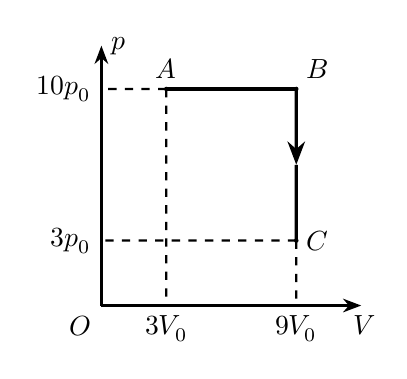
\begin{tikzpicture}[>=Stealth, scale=0.275, thick]
        % Hệ trục tọa độ
        \draw[->, thick] (0,0) -- (12,0) node[below] {$V$};
        \draw[->, thick] (0,0) -- (0,12) node[right] {$p$};
        \node[below left] at (0,0) {$O$};
        
        % Tọa độ các điểm
        \coordinate (A) at (3,10);
        \coordinate (B) at (9,10);
        \coordinate (C) at (9,3);
        
        % Đường dóng nét đứt
        \draw[dashed] (A) -- (3,0) node[below, black] {$3V_0$};
        \draw[dashed] (A) -- (0,10) node[left, black] {$10p_0$};
        \draw[dashed] (C) -- (9,0) node[below, black] {$9V_0$};
        \draw[dashed] (C) -- (0,3) node[left, black] {$3p_0$};
        
        % Các quá trình
        \draw[very thick] (A) -- (B);
        \draw[very thick, ->] (B) -- (9,6.5); % Mũi tên chỉ chiều B->C
        \draw[very thick] (9,6.5) -- (C);
        
        % Điểm nút
        \fill (A) circle (3pt) node[above] {$A$};
        \fill (B) circle (3pt) node[above right] {$B$};
        \fill (C) circle (3pt) node[right] {$C$};
        \end{tikzpicture}
    }
    \loigiai{
        \begin{itemchoice}
        \itemch  ${p_A V_A > p_C V_C \Rightarrow T_A > T_C}$.
        \itemch  ${A}$ sang ${B}$ là đẳng áp có ${V}$ tăng $\Rightarrow {T}$ tăng $\Rightarrow$ nội năng tăng.
        \itemch  ${A_{AB} = 10 p_0 \left(9 V_0 - 3 V_0\right) = 60 p_0 V_0}$.
        \itemch  ${B}$ đến ${C}$ là đẳng tích $\Rightarrow {A = 0}$ và có ${p}$ giảm $\Rightarrow {T}$ giảm $\Rightarrow$ nội năng giảm $\Rightarrow$ tỏa nhiệt.
        \end{itemchoice}
    }
\end{ex}


% Câu 4
\begin{ex}
    \immini[thm]{
        Như hình vẽ, một đoạn dây thẳng có khối lượng ${m}$ và chiều dài ${l}$ được treo vào hai điểm ${O}$ và ${O'}$ bằng hai sợi dây cách điện và được đặt trong một từ trường đều. Khi dòng điện ${I}$ chạy qua đoạn dây theo chiều dương trục ${x}$ và đoạn dây đứng yên, góc hợp bởi sợi dây treo và phương thẳng đứng là ${\theta}$. Gia tốc rơi tự do là ${g}$. Khi đó, hướng và độ lớn của cảm ứng từ có thể là
        \choiceTF
        {chiều dương trục ${z}$ và ${B = \frac{mg}{Il} \sin \theta}$}
        {chiều dương trục ${y}$ và ${B = \frac{mg}{Il}}$}
        {\True chiều âm trục ${z}$ và ${B = \frac{mg}{Il} \tan \theta}$}
        {dọc theo phương trục ${x}$ và ${B = \frac{mg}{Il} \sin \theta}$}
    }{
        \begin{tikzpicture}[>=Stealth, line cap=round, line join=round, scale=1.5, thick]          
            % 1. Đường treo cố định phía trên (từ trái qua phải, hơi dốc lên)
            \coordinate (O) at (0.4, 2.25);    % Điểm O nằm ở cột 1, hàng 2 (từ dưới lên)
            \coordinate (Op) at (2.6, 3.4);   % Điểm O' nằm ở cột 3, hàng 4
            \draw[thick] (-0.5, 1.8) -- (3.2, 3.7);
            
            \node[above] at (O) {$O$};
            \node[above] at (Op) {$O'$};

            % 2. Hệ trục tọa độ xyz (Gốc nằm ở giữa O và O', tại cột 2)
            \coordinate (Origin) at (1.55, 2.85); 
            \draw[->, thick] (Origin) -- (1.55, 3.8) node[right] {$z$}; % Trục z thẳng đứng
            \draw[->, thick] (Origin) -- (0.85, 2.5) node[below] {$x$}; % Trục x dọc theo đường treo
            \draw[->, thick] (Origin) -- (2.2, 2.4) node[below] {$y$}; % Trục y hướng ra ngoài

            % 3. Đường dóng thẳng đứng nét đứt từ O và O'
            \draw[dashed] (O) -- (0.4, 0.8) coordinate (V1);
            \draw[dashed] (Op) -- (2.6, 1.9) coordinate (V2);

            % 4. Dây treo và Thanh dẫn (nằm ở hàng 1 và 2)
            % Điểm kết nối trên thanh dẫn
            \coordinate (P1) at (1.3, 0.7); % Điểm treo dây trái trên thanh
            \coordinate (P2) at (3.45, 1.75); % Điểm treo dây phải trên thanh
            
            \draw[thick] (O) -- (P1);
            \draw[thick] (Op) -- (P2);

            % 5. Ký hiệu góc theta
            \pic [draw, "$\theta$", angle radius=0.8cm, angle eccentricity=1.4] {angle = V1--O--P1};
            \pic [draw, "$\theta$", angle radius=0.8cm, angle eccentricity=1.4] {angle = V2--Op--P2};

            % 6. Vẽ thanh dẫn hình trụ (Căn cứ vào hàng cuối của lưới đỏ)
            \begin{scope}
                \def\r{0.08}   % Bán kính thanh
                \def\ext{0.6}  % Độ dài phần thừa ra
                
                % Tính toán hướng của thanh dẫn (song song với đường treo)
                \coordinate (Start) at ($(P1) + ({-0.8*\ext}, -0.35)$);
                \coordinate (End) at ($(P2) + ({0.8*\ext}, 0.3)$);
                
                % Vẽ thân thanh trụ
                \filldraw[fill=white, thick] 
                    ($(Start) + (-0.02, \r)$) -- ($(End) + (-0.02, \r)$) 
                    arc (90:-90:{0.4*\r} and \r) -- ($(Start) + (-0.02, -\r)$) 
                    arc (270:90:{0.4*\r} and \r) -- cycle;

                % Mũi tên dòng điện I
                \draw[<-, thick] ($(Start)!0.35!(End)$) -- ($(Start)!0.65!(End)$) node[midway, above=2pt] {$I$};
            \end{scope}

        \end{tikzpicture}
    }
    \loigiai{
        Lực từ phải có xu hướng sang phải để đẩy sợi dây lệch về bên phải. Áp dụng quy tắc bàn tay trái
        \begin{itemchoice}
        \itemch 
        \itemch 
        \itemch  ${\tan \theta = \frac{F}{P} = \frac{BIl}{mg} \Rightarrow B = \frac{mg \tan \theta}{Il}}$.
        \itemch  Dọc theo phương trục ${x}$ thì ${B}$ cùng phương ${I}$ nên ${F = 0}$.
        \end{itemchoice}
    }
\end{ex}


% Câu 1
\begin{ex}
    Pha ${2 \, \mathrm{kg}}$ nước ở nhiệt độ ${10^\circ\mathrm{C}}$ với ${1 \, \mathrm{kg}}$ nước ở nhiệt độ ${70^\circ\mathrm{C}}$ thì thu được nước ở nhiệt độ bao nhiêu ${^\circ\mathrm{C}}$?
    \shortans{30}
    \loigiai{
        ${t = \frac{m_1 t_1 + m_2 t_2}{m_1 + m_2} = \frac{2 \cdot 10 + 1 \cdot 70}{2 + 1} = 30^\circ\mathrm{C}}$.
    }
\end{ex}


% Câu 2
\begin{ex}
    Một cuộn dây gồm ${200}$ vòng dây đặt trong từ trường. Độ biến thiên từ thông qua một vòng dây trong ${0{,}02 \, \mathrm{s}}$ là ${6 \cdot 10^{-5} \, \mathrm{Wb}}$. Độ lớn suất điện động cảm ứng trong cuộn dây là bao nhiêu ${\mathrm{V}}$ (kết quả làm tròn đến chữ số hàng phần mười)?
    \shortans{0,6}
    \loigiai{
        ${e = \left| \frac{N \Delta \phi}{\Delta t} \right| = \frac{200 \cdot 6 \cdot 10^{-5}}{0{,}02} = 0{,}6 \, \mathrm{V}}$.
    }
\end{ex}


% Câu 3
\begin{ex}
    Một bạn thường xuyên tắm sau khi tập thể dục. Lưu lượng nước tắm lấy từ bình nóng điện là ${10 \, \mathrm{lít/phút}}$ và thời gian bạn tắm là ${4}$ phút. Bình nóng điện sử dụng điện áp ${220 \, \mathrm{V}}$ và cường độ dòng điện ${10 \, \mathrm{A}}$ để làm nóng nước từ nhiệt độ ban đầu ${20^\circ\mathrm{C}}$ lên tới nhiệt độ ${50^\circ\mathrm{C}}$. Hiệu suất đun nóng của bình là ${80\%}$, nước có khối lượng riêng là ${1000 \, \mathrm{kg/m^3}}$ và nhiệt dung riêng là ${4200 \, \mathrm{J/(kg \cdot K)}}$. Thời gian đun nóng nước trong bình ít nhất là bao nhiêu phút (làm tròn kết quả đến chữ số hàng phần mười)?
    \shortans{47,7}
    \loigiai{
        ${m = VD = 10 \cdot 10^{-3} \cdot 4 \cdot 1000 = 40 \, \mathrm{kg}}$.\\
        ${Q = mc \Delta t = 40 \cdot 4200 \cdot \left(50 - 20\right) = 5{,}04 \cdot 10^6 \, \mathrm{J}}$.\\
        ${A = \frac{Q}{H} = \frac{5{,}04 \cdot 10^6}{0{,}8} = 6{,}3 \cdot 10^6 \, \mathrm{J}}$.\\
        ${P = UI = 220 \cdot 10 = 2200 \, \mathrm{W}}$.\\
        ${t = \frac{A}{P} = \frac{6{,}3 \cdot 10^6}{2200} \approx 2864 \, \mathrm{s} \approx 47{,}7}$ phút.
    }
\end{ex}


% Câu 4
\begin{ex}
    \immini[thm]{
        Hình bên là cấu trúc tinh thể caesium clorua ($\mathrm{CsCl}$): ion $\mathrm{Cl^-}$ (chấm trắng) nằm ở tâm của khối lập phương và ion $\mathrm{Cs^+}$ (chấm đen) nằm ở tám đỉnh của khối lập phương. Biết khối lượng mol của caesium clorua là ${168 \, \mathrm{g/mol}}$, khoảng cách gần nhất giữa hai ion $\mathrm{Cl^-}$ là ${4 \cdot 10^{-10} \, \mathrm{m}}$. Lấy ${N_A = 6{,}02 \cdot 10^{23} \, \mathrm{mol^{-1}}}$. Khối lượng riêng của caesium clorua là bao nhiêu ${\mathrm{g/cm^3}}$ (làm tròn kết quả đến chữ số hàng phần mười)?
    }{
        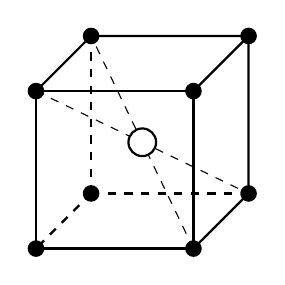
\begin{tikzpicture}[scale=2]
            % Định nghĩa các đỉnh của hình lập phương
            \def\s{0.35} % Độ xiên
            \coordinate (A) at (0,0);      % Trước - Dưới - Trái
            \coordinate (B) at (1,0);      % Trước - Dưới - Phải
            \coordinate (C) at (1,1);      % Trước - Trên - Phải
            \coordinate (D) at (0,1);      % Trước - Trên - Trái
            \coordinate (E) at (\s,\s);    % Sau   - Dưới - Trái
            \coordinate (F) at (1+\s,\s);  % Sau   - Dưới - Phải
            \coordinate (G) at (1+\s,1+\s);% Sau   - Trên - Phải
            \coordinate (H) at (\s,1+\s);  % Sau   - Trên - Trái
            \coordinate (Center) at (0.5+\s/2, 0.5+\s/2);

            % Các cạnh khuất (nét đứt)
            \draw[dashed, thick] (E) -- (F);
            \draw[dashed, thick] (E) -- (H);
            \draw[dashed, thick] (E) -- (A);
            
            % Các đường chéo thân (nét đứt)
            \draw[dashed] (B) -- (H);
            \draw[dashed] (D) -- (F);

            % Các cạnh nhìn thấy
            \draw[thick] (A) -- (B) -- (C) -- (D) -- cycle;
            \draw[thick] (B) -- (F) -- (G) -- (C);
            \draw[thick] (D) -- (H) -- (G);

            % Nguyên tử tại các đỉnh (chấm đen)
            \foreach \p in {A,B,C,D,E,F,G,H} \fill (\p) circle (1.5pt);

            % Nguyên tử tại tâm (vòng tròn trắng viền đen)
            \draw[thick, fill=white] (Center) circle (2.5pt);
        \end{tikzpicture}
    }
    \shortans{4,4}
    \loigiai{
        ${D = \frac{m}{V} = \frac{M}{N_A a^3} = \frac{168 \cdot 10^{-3}}{6{,}02 \cdot 10^{23} \cdot \left(4{,}10 \cdot 10^{-10}\right)^3} \approx 4{,}4 \cdot 10^3 \, \mathrm{kg/m^3} = 4{,}4 \, \mathrm{g/cm^3}}$.
    }
\end{ex}


% Câu 5
\begin{ex}
    \immini[thm]{
        Khinh khí cầu gồm ba phần: bóng khí cầu, giỏ và thiết bị sưởi ấm. Khí cầu có một lỗ ở đáy để không khí lưu thông giữa bên trong và bên ngoài. Bên trong khí cầu có một bộ điều nhiệt giúp điều chỉnh nhiệt độ của không khí bên trong, điều khiển sự lên xuống của khí cầu. Tổng khối lượng của khinh khí cầu là ${600 \, \mathrm{kg}}$ (không tính khối lượng không khí bên trong khinh khí cầu). Thể tích của khinh khí cầu luôn là ${2000 \, \mathrm{m^3}}$ (bỏ qua độ dày của vỏ khinh khí cầu và thể tích giỏ treo). Không khí bên ngoài có nhiệt độ là ${15^\circ\mathrm{C}}$ và khối lượng riêng là ${1{,}2 \, \mathrm{kg/m^3}}$. Hỏi nhiệt độ bên trong khinh khí cầu cần phải nâng lên bao nhiêu ${^\circ\mathrm{C}}$ để khinh khí cầu bắt đầu bay lên (kết quả làm tròn đến chữ số hàng đơn vị)?
    }{
        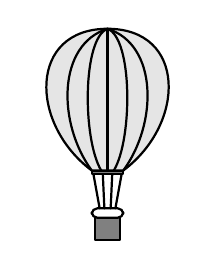
\begin{tikzpicture}[line join=round, line cap=round, thick, scale=0.4]

            % --- 1. VẼ GIỎ (BASKET) ---
            % Phần thân dưới của giỏ
            \draw[fill=gray] (-0.4, -2.5) -- (-0.4, -3.2) -- (0.4, -3.2) -- (0.4, -2.5);
            % Vành miệng giỏ (Phần nhô ra)
            \draw[rounded corners=2pt] (-0.5, -2.5) rectangle (0.5, -2.2);

            % --- 2. VẼ DÂY TREO (CABLES) ---
            % Các đường thẳng nối từ thân khinh khí cầu xuống giỏ
            \draw (-0.45, -1.1) -- (-0.25, -2.2);
            \draw (-0.15, -1.1) -- (-0.1, -2.2);
            \draw (0.15, -1.1) -- (0.1, -2.2);
            \draw (0.45, -1.1) -- (0.25, -2.2);

            % --- 3. VẼ ĐẾ KHINH KHÍ CẦU (RING/SKIRT) ---
            \draw[fill=gray] (-0.5, -1.1) rectangle (0.5, -1.0);

            % --- 4. VẼ QUẢ BÓNG CHÍNH (ENVELOPE) ---
            % Đường viền bao ngoài quả bóng
            \draw[fill=gray!20] (0, 3.5) .. controls (-2.5, 3.5) and (-2.5, 0.5) .. (-0.5, -1)
                (0, 3.5) .. controls (2.5, 3.5) and (2.5, 0.5) .. (0.5, -1) -- (-0.5, -1);

            % Các đường gân dọc (Gores) tạo khối 3D cho khinh khí cầu
            % Đường trung tâm
            \draw (0, 3.5) -- (0, -1);
            
            % Các đường cong bên trái
            \draw (0, 3.5) .. controls (-0.8, 3.2) and (-0.8, 0) .. (-0.2, -1);
            \draw (0, 3.5) .. controls (-1.6, 3) and (-1.6, 0.5) .. (-0.5, -1);

            % Các đường cong bên phải
            \draw (0, 3.5) .. controls (0.8, 3.2) and (0.8, 0) .. (0.2, -1);
            \draw (0, 3.5) .. controls (1.6, 3) and (1.6, 0.5) .. (0.5, -1);

        \end{tikzpicture}
    }
    \shortans{111}
    \loigiai{
        ${F_A = P \Rightarrow D_{kq} V g = mg + D V g \Rightarrow 1{,}2 \cdot 2000 = 600 + D \cdot 2000 \Rightarrow D = 0{,}9 \, \mathrm{kg/m^3}}$.\\
        ${\frac{p}{DT} = \frac{R}{M} \Rightarrow DT = \text{const} \Rightarrow 1{,}2 \cdot \left(15 + 273\right) = 0{,}9 \cdot T \Rightarrow T = 384 \, \mathrm{K} = 111^\circ\mathrm{C}}$.
    }
\end{ex}


% Câu 6
\begin{ex}
    \immini[thm]{
        Một ống thủy tinh kín hai đầu chứa một đoạn thủy ngân, khi đặt ống nằm ngang thì cột không khí ở hai đầu có chiều dài bằng nhau và có cùng áp suất là ${80 \, \mathrm{cmHg}}$. Khi ống đặt thẳng đứng thì chiều dài cột không khí phía trên gấp ${2}$ lần cột không khí phía dưới. Coi nhiệt độ các cột không khí không đổi. Chiều dài đoạn thủy ngân trong ống bằng bao nhiêu ${\mathrm{cm}}$ (kết quả làm tròn đến chữ số hàng đơn vị)?
    }{
        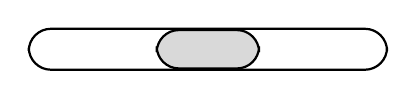
\begin{tikzpicture}[thick, scale = 0.65]
        % Vẽ vỏ ống thủy tinh
        \draw[thick, rounded corners=8pt] (0,0) rectangle (7,0.8);
        
        % Vẽ cột chất lỏng ở giữa
        \filldraw[fill=gray!30, draw=black, thick, rounded corners=8pt] (2.5,0.025) rectangle (4.5,0.775);
        \end{tikzpicture}
    }
    \shortans{60}
    \loigiai{
        Khi ống thẳng đứng thì ${V_1 = 2 V_2 \Rightarrow}$ chuẩn hóa ${V_1 = 2}$ và ${V_2 = 1 \Rightarrow V_0 = \frac{V_1 + V_2}{2} = \frac{2 + 1}{2} = 1{,}5}$.\\
        ${p_0 V_0 = p_1 V_1 = p_2 V_2 \Rightarrow 80 \cdot 1{,}5 = p_1 \cdot 2 = p_2 \cdot 1 \Rightarrow \left\{\begin{aligned} & p_1 = 60 \, \mathrm{cmHg} \\ & p_2 = 120 \, \mathrm{cmHg} \end{aligned}\right.}$.\\
        ${h = p_2 - p_1 = 120 - 60 = 60 \, \mathrm{cm}}$.
    }
\end{ex}

% Câu 1
\begin{ex}
    Hạt nhân nào sau đây có thể phân hạch
    \choice
    {${^{12}_{6}\mathrm{C}}$}
    {${^{14}_{7}\mathrm{N}}$}
    {\True ${^{239}_{94}\mathrm{Pu}}$}
    {${^{7}_{3}\mathrm{Li}}$}
    \loigiai{
    }
\end{ex}


% Câu 2
\begin{ex}
    Trong một phản ứng hạt nhân, có sự bảo toàn
    \choice
    {số proton}
    {\True số nucleon}
    {số neutron}
    {khối lượng}
    \loigiai{
    }
\end{ex}


% Câu 3
\begin{ex}
    Trong phản ứng hạt nhân không có sự bảo toàn
    \choice
    {số nucleon}
    {động lượng}
    {\True số neutron}
    {năng lượng toàn phần}
    \loigiai{
    }
\end{ex}


% Câu 4
\begin{ex}
    Trong phản ứng hạt nhân, không có sự bảo toàn
    \choice
    {\True khối lượng}
    {động lượng}
    {số nucleon}
    {năng lượng toàn phần}
    \loigiai{
    }
\end{ex}


% Câu 5
\begin{ex}
    Cho phản ứng hạt nhân: ${^{2}_{1}\mathrm{H} + ^{3}_{1}\mathrm{H} \rightarrow ^{4}_{2}\mathrm{He} + ^{1}_{0}\mathrm{n}}$. Đây là
    \choice
    {phản ứng phân hạch}
    {phản ứng thu năng lượng}
    {\True phản ứng nhiệt hạch}
    {hiện tượng phóng xạ hạt nhân}
    \loigiai{
    }
\end{ex}


% Câu 6
\begin{ex}
    Cho phản ứng hạt nhân ${^{1}_{0}\mathrm{n} + ^{235}_{92}\mathrm{U} \rightarrow ^{94}_{38}\mathrm{Sr} + ^{140}_{54}\mathrm{Xe} + 2 ^{1}_{0}\mathrm{n}}$. Đây là
    \choice
    {\True phản ứng phân hạch}
    {phản ứng thu năng lượng}
    {phản ứng nhiệt hạch}
    {quá trình phóng xạ}
    \loigiai{
    }
\end{ex}


% Câu 7
\begin{ex}
    Phản ứng hạt nhân nào sau đây không phải là phản ứng nhiệt hạch?
    \choice
    {${^{1}_{1}\mathrm{H} + ^{3}_{1}\mathrm{H} \rightarrow ^{4}_{2}\mathrm{He}}$}
    {${^{2}_{1}\mathrm{H} + ^{2}_{1}\mathrm{H} \rightarrow ^{4}_{2}\mathrm{He}}$}
    {${^{2}_{1}\mathrm{H} + ^{3}_{1}\mathrm{H} \rightarrow ^{4}_{2}\mathrm{He} + ^{1}_{0}\mathrm{n}}$}
    {\True ${^{210}_{84}\mathrm{Po} \rightarrow ^{4}_{2}\mathrm{He} + ^{206}_{82}\mathrm{Pb}}$}
    \loigiai{
    }
\end{ex}


% Câu 8
\begin{ex}
    Phản ứng nhiệt hạch là
    \choice
    {sự kết hợp hai hạt nhân có số khối trung bình tạo thành hạt nhân nặng hơn}
    {phản ứng hạt nhân thu năng lượng}
    {phản ứng trong đó một hạt nhân nặng vỡ thành hai mảnh nhẹ hơn}
    {\True phản ứng hạt nhân tỏa năng lượng}
    \loigiai{
    }
\end{ex}


% Câu 9
\begin{ex}
    Cho phản ứng hạt nhân ${^{1}_{0}\mathrm{n} + ^{235}_{92}\mathrm{U} \rightarrow ^{94}_{38}\mathrm{Sr} + \mathrm{X} + 2 ^{1}_{0}\mathrm{n}}$. Hạt nhân $\mathrm{X}$ có cấu tạo gồm:
    \choice
    {\True ${54}$ proton và ${86}$ neutron}
    {${54}$ proton và ${140}$ neutron}
    {${86}$ proton và ${140}$ neutron}
    {${86}$ proton và ${54}$ neutron}
    \loigiai{
        $\begin{cases} 1 + 235 = 94 + A + 2 \\ 92 = 38 + Z \end{cases} \Rightarrow \begin{cases} A = 140 \\ Z = 54 \end{cases} \Rightarrow N = A - Z = 140 - 54 = 86$.
    }
\end{ex}


% Câu 10
\begin{ex}
    Giả sử trong một phản ứng hạt nhân, tổng khối lượng của các hạt trước phản ứng nhỏ hơn tổng khối lượng các hạt sau phản ứng là ${0{,}02 \, \mathrm{amu}}$. Phản ứng hạt nhân này
    \choice
    {\True thu năng lượng ${18{,}63 \, \mathrm{MeV}}$}
    {thu năng lượng ${1{,}863 \, \mathrm{MeV}}$}
    {tỏa năng lượng ${1{,}863 \, \mathrm{MeV}}$}
    {tỏa năng lượng ${18{,}63 \, \mathrm{MeV}}$}
    \loigiai{
        $\Delta E = \left(m_t - m_s\right) c^2 = -0{,}02 \cdot 931{,}5 = -18{,}63 \, \mathrm{MeV} < 0$.
    }
\end{ex}


% Câu 11
\begin{ex}
    Cho phản ứng hạt nhân: ${^{2}_{1}\mathrm{D} + ^{2}_{1}\mathrm{D} \rightarrow ^{3}_{2}\mathrm{He} + ^{1}_{0}\mathrm{n}}$. Biết khối lượng các hạt nhân ${^{2}_{1}\mathrm{D}}$, ${^{3}_{2}\mathrm{He}}$, ${^{1}_{0}\mathrm{n}}$ lần lượt là ${2{,}0135 \, \mathrm{amu}}$; ${3{,}0149 \, \mathrm{amu}}$; ${1{,}0087 \, \mathrm{amu}}$. Năng lượng tỏa ra của phản ứng trên bằng
    \choice
    {${1{,}8821 \, \mathrm{MeV}}$}
    {${2{,}7391 \, \mathrm{MeV}}$}
    {${7{,}4991 \, \mathrm{MeV}}$}
    {\True ${3{,}1671 \, \mathrm{MeV}}$}
    \loigiai{
        $\Delta E = \left(2m_D - m_{He} - m_n\right) c^2 = \left(2 \cdot 2{,}0135 - 3{,}0149 - 1{,}0087\right) \cdot 931{,}5 = 3{,}1671 \, \mathrm{MeV}$.
    }
\end{ex}


% Câu 12
\begin{ex}
    Cho phản ứng hạt nhân: ${^{3}_{1}\mathrm{T} + ^{2}_{1}\mathrm{D} \rightarrow ^{4}_{2}\mathrm{He} + \mathrm{X}}$. Lấy độ hụt khối của hạt nhân $\mathrm{T}$, hạt nhân $\mathrm{D}$, hạt nhân $\mathrm{He}$ lần lượt là ${0{,}009106 \, \mathrm{amu}}$; ${0{,}002491 \, \mathrm{amu}}$; ${0{,}030382 \, \mathrm{amu}}$. Năng lượng tỏa ra của phản ứng là
    \choice
    {${15{,}017 \, \mathrm{MeV}}$}
    {${200{,}025 \, \mathrm{MeV}}$}
    {\True ${17{,}498 \, \mathrm{MeV}}$}
    {${21{,}076 \, \mathrm{MeV}}$}
    \loigiai{
        $\Delta E = \left(\Delta m_s - \Delta m_t\right) c^2 = \left(0{,}030382 - 0{,}009106 - 0{,}002491\right) \cdot 931{,}5 \approx 17{,}498 \, \mathrm{MeV}$.
    }
\end{ex}


% Câu 13
\begin{ex}
    Dùng hạt proton có động năng ${5{,}45 \, \mathrm{MeV}}$ bắn vào hạt nhân ${^{9}_{4}\mathrm{Be}}$ đứng yên gây ra phản ứng: $\mathrm{p} + {^{9}_{4}\mathrm{Be}} \rightarrow \mathrm{X} + {^{6}_{3}\mathrm{Li}}$. Biết động năng của hạt $\mathrm{X}$ và ${^{6}_{3}\mathrm{Li}}$ lần lượt là ${4 \, \mathrm{MeV}}$ và ${3{,}575 \, \mathrm{MeV}}$. Phản ứng hạt nhân này
    \choice
    {tỏa ${1{,}463 \, \mathrm{MeV}}$}
    {thu ${3{,}0072 \, \mathrm{MeV}}$}
    {\True tỏa ${2{,}125 \, \mathrm{MeV}}$}
    {thu ${29{,}069 \, \mathrm{MeV}}$}
    \loigiai{
        $\Delta E = K_X + K_{Li} - K_p = 4 + 3{,}575 - 5{,}45 = 2{,}125 \, \mathrm{MeV}$.
    }
\end{ex}


% Câu 14
\begin{ex}
    Dùng hạt proton bắn vào hạt nhân ${^{7}_{3}\mathrm{Li}}$ đứng yên. Sau phản ứng sinh ra hai hạt nhân $\mathrm{X}$ có động năng bằng nhau và bằng ${9{,}343 \, \mathrm{MeV}}$. Năng lượng tỏa ra của phản ứng này là ${17{,}2235 \, \mathrm{MeV}}$. Động năng của hạt proton là
    \choice
    {\True ${1{,}4625 \, \mathrm{MeV}}$}
    {${3{,}0072 \, \mathrm{MeV}}$}
    {${1{,}5032 \, \mathrm{MeV}}$}
    {${29{,}0693 \, \mathrm{MeV}}$}
    \loigiai{
        $\Delta E = 2K_X - K_p \Rightarrow 17{,}2235 = 2 \cdot 9{,}343 - K_p \Rightarrow K_p = 1{,}4625 \, \mathrm{MeV}$.
    }
\end{ex}


% Câu 15
\begin{ex}
    Cho phản ứng hạt nhân: ${^{1}_{1}\mathrm{p} + ^{7}_{3}\mathrm{Li} \rightarrow \mathrm{X} + ^{4}_{2}\mathrm{He} + 17{,}3 \, \mathrm{MeV}}$. Năng lượng tỏa ra khi tổng hợp được ${1 \, \mathrm{g}}$ khí helium là
    \choice
    {${26{,}04 \cdot 10^{26} \, \mathrm{MeV}}$}
    {${13{,}02 \cdot 10^{26} \, \mathrm{MeV}}$}
    {\True ${13{,}02 \cdot 10^{23} \, \mathrm{MeV}}$}
    {${26{,}04 \cdot 10^{23} \, \mathrm{MeV}}$}
    \loigiai{
        ${^{1}_{1}\mathrm{p} + ^{7}_{3}\mathrm{Li} \rightarrow ^{4}_{2}\mathrm{He} + ^{4}_{2}\mathrm{He}}$ \\
        $n_{He} = \frac{m}{M} = \frac{1}{4} = 0{,}25 \, \mathrm{mol}$ \\
        $N_{He} = n_{He} N_A = 0{,}25 \cdot 6{,}02 \cdot 10^{23} = 1{,}505 \cdot 10^{23}$ \\
        $N = \frac{N_{He}}{2} = \frac{1{,}505 \cdot 10^{23}}{2} = 7{,}525 \cdot 10^{22}$ \\
        $Q = N \Delta E = 7{,}525 \cdot 10^{22} \cdot 17{,}3 \approx 13{,}02 \cdot 10^{23} \, \mathrm{MeV}$.
    }
\end{ex}


% Câu 16
\begin{ex}
    Một lò phản ứng phân hạch có công suất ${200 \, \mathrm{MW}}$. Cho rằng toàn bộ năng lượng mà lò phản ứng này sinh ra đều do sự phân hạch của ${^{235}\mathrm{U}}$ và đồng vị này chỉ bị tiêu hao bởi quá trình phân hạch. Coi mỗi năm có ${365}$ ngày; mỗi phân hạch sinh ra ${200 \, \mathrm{MeV}}$. Khối lượng ${^{235}\mathrm{U}}$ mà lò phản ứng tiêu thụ trong ${3}$ năm là
    \choice
    {${461{,}6 \, \mathrm{g}}$}
    {${461{,}6 \, \mathrm{kg}}$}
    {\True ${230{,}8 \, \mathrm{kg}}$}
    {${230{,}8 \, \mathrm{g}}$}
    \loigiai{
        $Q = Pt = 200 \cdot 10^6 \cdot 3 \cdot 365 \cdot 24 \cdot 60 \cdot 60 = 1{,}89216 \cdot 10^{16} \, \mathrm{J}$ \\
        $N = \frac{Q}{\Delta E} = \frac{1{,}89216 \cdot 10^{16}}{200 \cdot 1{,}6 \cdot 10^{-13}} = 5{,}913 \cdot 10^{26}$ \\
        $n = \frac{N}{N_A} = \frac{5{,}913 \cdot 10^{26}}{6{,}02 \cdot 10^{23}} \approx 982 \, \mathrm{mol}$ \\
        $m = n M = 982 \cdot 235 = 230{,}8 \cdot 10^3 \, \mathrm{g} = 230{,}8 \, \mathrm{kg}$.
    }
\end{ex}


% Câu 17
\begin{ex}
    Người ta dự định xây một nhà máy điện nguyên tử có công suất bằng công suất tối đa của nhà máy thủy điện Hòa Bình (${1{,}92}$ triệu $\mathrm{kW}$). Giả sử các lò phản ứng dùng năng lượng phân hạch của hạt nhân ${^{235}\mathrm{U}}$ với hiệu suất ${20\%}$ và trung bình mỗi hạt ${^{235}\mathrm{U}}$ phân hạch tỏa ra năng lượng ${200 \, \mathrm{MeV}}$. Lấy $N_A = {6{,}02 \cdot 10^{23}}$. Coi khối lượng nguyên tử tính theo $\mathrm{amu}$ bằng số khối của nó. Khối lượng ${^{235}\mathrm{U}}$ nguyên chất cần cho các lò phản ứng trong thời gian ${1}$ năm (${365}$ ngày) có giá trị gần nhất với giá trị nào sau đây?
    \choice
    {${5900 \, \mathrm{kg}}$}
    {${1200 \, \mathrm{kg}}$}
    {${740 \, \mathrm{kg}}$}
    {\True ${3700 \, \mathrm{kg}}$}
    \loigiai{
        $W = Pt = 1{,}92 \cdot 10^9 \cdot 365 \cdot 24 \cdot 60 \cdot 60 = 6{,}054912 \cdot 10^{16} \, \mathrm{J}$ \\
        $Q = \frac{W}{H} = \frac{6{,}054912 \cdot 10^{16}}{0{,}2} = 3{,}027456 \cdot 10^{17} \, \mathrm{J}$ \\
        $N = \frac{Q}{\Delta E} = \frac{3{,}027456 \cdot 10^{17}}{200 \cdot 1{,}6 \cdot 10^{-13}} = 9{,}4608 \cdot 10^{27}$ \\
        $n = \frac{N}{N_A} = \frac{9{,}4608 \cdot 10^{27}}{6{,}02 \cdot 10^{23}} \approx 15716 \, \mathrm{mol}$ \\
        $m = n M = 15716 \cdot 235 \approx 3{,}7 \cdot 10^6 \, \mathrm{g} = 3{,}7 \cdot 10^3 \, \mathrm{kg}$.
    }
\end{ex}


% Câu 18
\begin{ex}
    Để tăng cường sức mạnh hải quân, Việt Nam đã đặt mua của Nga ${6}$ tàu ngầm hiện đại lớp Ki-lô: HQ-182 Hà Nội, HQ-183 Hồ Chí Minh,... Trong đó HQ-182 Hà Nội có công suất của động cơ là ${4400 \, \mathrm{kW}}$ chạy bằng điêzen-điện. Giả sử động cơ trên dùng năng lượng phân hạch của hạt nhân ${^{235}\mathrm{U}}$ với hiệu suất ${20\%}$ và trung bình mỗi hạt ${^{235}\mathrm{U}}$ phân hạch tỏa ra năng lượng ${200 \, \mathrm{MeV}}$. Lấy $N_A = {6{,}02 \cdot 10^{23}}$. Coi khối lượng nguyên tử tính theo $\mathrm{amu}$ bằng số khối của nó. Thời gian tiêu thụ hết ${0{,}8 \, \mathrm{kg}}$ ${^{235}\mathrm{U}}$ nguyên chất có giá trị gần nhất với giá trị nào sau đây?
    \choice
    {${19{,}9}$ ngày}
    {${21{,}6}$ ngày}
    {${18{,}6}$ ngày}
    {\True ${34}$ ngày}
    \loigiai{
        $t = \frac{W}{P} = \frac{\dfrac{m}{M} \cdot N_A \cdot \Delta E \cdot H}{P} = \frac{\dfrac{0{,}8 \cdot 10^3}{235} \cdot 6{,}02 \cdot 10^{23} \cdot 200 \cdot 1{,}6 \cdot 10^{-13} \cdot 0{,}2}{4400 \cdot 10^3} \approx 2{,}98 \cdot 10^6 \, \mathrm{s} \approx 34{,}5$ ngày.
    }
\end{ex}


% Câu 1
\begin{ex}
    Sự phân hạch của các nguyên tố nặng được khám phá thực nghiệm vào tháng 12 năm 1938. Lí thuyết về phản ứng nhiệt hạch bắt đầu được xây dựng vào thập niên 1920. Cho đến nay, con người đã có những tiến bộ rất lớn trong việc tìm hiểu và ứng dụng những phản ứng hạt nhân này.
    \choiceTF
    {\True Ngày nay, phản ứng phân hạch được khai thác trong lò phản ứng của các nhà máy điện hạt nhân trên thế giới}
    {Phản ứng nhiệt hạch xảy ra trong lõi của Trái Đất, nó là nguồn gốc năng lượng địa nhiệt của Trái Đất}
    {\True Phản ứng phân hạch và phản ứng nhiệt hạch đều là phản ứng hạt nhân kích thích và tỏa năng lượng}
    {\True Cho đến nay, con người chưa điều khiển được phản ứng nhiệt hạch để phát điện}
    \loigiai{
        \begin{itemchoice}
        \itemch 
        \itemch Năng lượng địa nhiệt của Trái Đất chủ yếu đến từ sự phân rã phóng xạ của các nguyên tố như uranium, thorium và kali, cùng với nhiệt dư từ quá trình hình thành Trái Đất. Phản ứng nhiệt hạch (fusion) chỉ xảy ra trong lòng các ngôi sao như Mặt Trời, không phải trong lõi Trái Đất.
        \itemch 
        \itemch 
        \end{itemchoice}
    }
\end{ex}


% Câu 2
\begin{ex}
    Hình sau mô tả một phản ứng hạt nhân.
    \begin{center}
        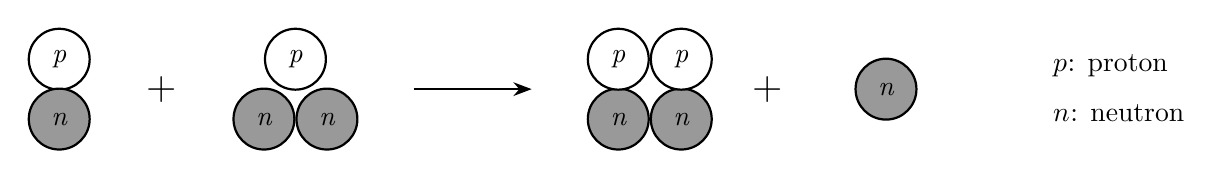
\begin{tikzpicture}[>=Stealth, thick]
            % --- Định nghĩa style cho proton (p) và neutron (n) ---
            \tikzset{
                pNode/.style={circle, draw, fill=white, minimum size=22pt, inner sep=0pt, font=\itshape},
                nNode/.style={circle, draw, fill=gray!80, minimum size=22pt, inner sep=0pt, font=\itshape}
            }

            % --- Vế trái: Các hạt tham gia phản ứng ---
            % Hạt nhân Đơteri (1p, 1n)
            \begin{scope}[shift={(0,0)}]
                \node[pNode] at (0, 0.38) {p};
                \node[nNode] at (0, -0.38) {n};
            \end{scope}

            % Dấu cộng thứ nhất
            \node at (1.3, 0) {\Large +};

            % Hạt nhân Triti (1p, 2n)
            \begin{scope}[shift={(3.0,0)}]
                \node[nNode] at (-0.4, -0.38) {n};
                \node[nNode] at (0.4, -0.38) {n};
                \node[pNode] at (0, 0.38) {p};
            \end{scope}

            % --- Mũi tên phản ứng ---
            \draw[->, thick] (4.5, 0) -- (6.0, 0);

            % --- Vế phải: Sản phẩm phản ứng ---
            % Hạt nhân Heli (Alpha - 2p, 2n)
            \begin{scope}[shift={(7.5,0)}]
                \node[nNode] at (-0.4, -0.38) {n};
                \node[nNode] at (0.4, -0.38) {n};
                \node[pNode] at (-0.4, 0.38) {p};
                \node[pNode] at (0.4, 0.38) {p};
            \end{scope}

            % Dấu cộng thứ hai
            \node at (9.0, 0) {\Large +};

            % Neutron tự do
            \begin{scope}[shift={(10.5,0)}]
                \node[nNode] at (0, 0) {n};
            \end{scope}

            % --- Chú thích (Legend) ---
            \begin{scope}[shift={(12.5,0)}]
                \node[anchor=west] at (0, 0.3) {$p$: proton};
                \node[anchor=west] at (0, -0.3) {$n$: neutron};
            \end{scope}

        \end{tikzpicture}
    \end{center}
    Năng lượng tỏa ra trong phản ứng trên là ${17{,}3 \, \mathrm{MeV}}$.
    \choiceTF
    {\True Hai hạt nhân tương tác (trước phản ứng) là đồng vị của hydrogen}
    {\True Phản ứng trên là phản ứng tổng hợp hạt nhân}
    {Phương trình của phản ứng là ${^{1}_{1}\mathrm{H} + ^{2}_{1}\mathrm{H} \rightarrow ^{3}_{2}\mathrm{He} + ^{1}_{0}\mathrm{n}}$}
    {Nếu có ${1}$ gam helium được tạo ra thì năng lượng tỏa ra là ${2{,}15 \cdot 10^{20} \, \mathrm{J}}$}
    \loigiai{
        \begin{itemchoice}
        \itemch Vì đều có ${1}$ proton.
        \itemch 
        \itemch ${^{2}_{1}\mathrm{H} + ^{3}_{1}\mathrm{H} \rightarrow ^{4}_{2}\mathrm{He} + ^{1}_{0}\mathrm{n}}$.
        \itemch $n = \frac{m}{M} = \frac{1}{4} = 0{,}25 \, \mathrm{mol}$ \\
        $N = n N_A = 0{,}25 \cdot 6{,}02 \cdot 10^{23} = 1{,}505 \cdot 10^{23}$ \\
        $Q = N \Delta E = 1{,}505 \cdot 10^{23} \cdot 17{,}3 \cdot 1{,}6 \cdot 10^{-13} \approx 4{,}17 \cdot 10^{11} \, \mathrm{J}$.
        \end{itemchoice}
    }
\end{ex}


% Câu 3
\begin{ex}
    Một nhà máy điện hạt nhân dùng nhiên liệu uranium ${^{235}_{92}\mathrm{U}}$. Biết công suất phát điện là ${550 \, \mathrm{MW}}$ và hiệu suất chuyển hóa năng lượng hạt nhân thành điện năng là ${20\%}$. Cho rằng một hạt nhân uranium ${^{235}_{92}\mathrm{U}}$ phân hạch thì tỏa ra năng lượng là ${3{,}2 \cdot 10^{-11} \, \mathrm{J}}$. Cho biết khối lượng mol của ${^{235}_{92}\mathrm{U}}$ là ${235 \, \mathrm{g/mol}}$.
    \choiceTF
    {\True Loại phản ứng hạt nhân được khai thác bên trong các nhà máy điện hạt nhân ngày nay là phản ứng phân hạch}
    {\True Năng lượng ${1}$ gam ${^{235}_{92}\mathrm{U}}$ phân hạch tỏa ra là ${5{,}1 \cdot 10^{23} \, \mathrm{MeV}}$}
    {Năng lượng điện nhà máy cung cấp trong ${1}$ giờ là ${1{,}89 \cdot 10^{12} \, \mathrm{J}}$}
    {Nếu nhà máy hoạt động liên tục thì lượng Uranium $^{235}_{92}\mathrm{U}$ mà nhà máy cần dùng trong $365$ ngày gần bằng $962\,\mathrm{kg}$}
    \loigiai{
        \begin{itemchoice}
        \itemch 
        \itemch $n = \frac{m}{M} = \frac{1}{235}\,\mathrm{mol}$\\
        $N = nN_A = \frac{1}{235} \cdot 6{,}02 \cdot 10^{23} \approx 2{,}562 \cdot 10^{21}$\\
        $Q = N\Delta E = 2{,}562 \cdot 10^{21} \cdot 3{,}2 \cdot 10^{-11} \approx 8{,}2 \cdot 10^{10}\,\mathrm{J} \approx 5{,}12 \cdot 10^{23}\,\mathrm{MeV}$
        \itemch Trong $1$ giờ: $A = Pt = 550 \cdot 10^{6} \cdot 60 \cdot 60 = 1{,}98 \cdot 10^{12}\,\mathrm{J}$
        \itemch Trong $365$ ngày: \\
        $A_d = A \cdot 365 \cdot 24 = 1{,}98 \cdot 10^{12} \cdot 365 \cdot 24 = 1{,}73448 \cdot 10^{16}\,\mathrm{J}$\\
        $Q_d = \frac{A_d}{H} = \frac{1{,}73448 \cdot 10^{16}}{0{,}2} = 8{,}6724 \cdot 10^{16}\,\mathrm{J}$\\
        $m = \frac{Q_d}{Q} = \frac{8{,}6724 \cdot 10^{16}}{8{,}2 \cdot 10^{10}} \approx 1058 \cdot 10^{3}\,\mathrm{g} = 1058\,\mathrm{kg}$
        \end{itemchoice}
    }
\end{ex}


% Câu 4
\begin{ex}
\immini[thm]{
    Hình bên cho một sơ đồ khái quát về một nhà máy điện dựa trên loại lò phản ứng nước nén. Một nhà máy phát điện cỡ lớn hoạt động dựa trên một lò phản ứng hạt nhân kiểu nước nén. Công suất nhiệt trong vùng hoạt động của lò phản ứng là ${3400 \, \mathrm{MW}}$, công suất điện được tạo ra là ${1100 \, \mathrm{MW}}$. Nhiên liệu là ${86000 \, \mathrm{kg}}$ uranium (gồm $^{238}_{92}\mathrm{U}$ và $^{235}_{92}\mathrm{U}$ được tách từ quặng oxit uranium) được phân bố trong ${57000}$ thanh nhiên liệu, Uranium được làm giàu tới ${2{,}98\%} \, ^{235}_{92}\mathrm{U}$ (tỉ lệ về khối lượng). $^{235}_{92}\mathrm{U}$ có chu kì bán rã là ${703{,}8}$ triệu năm, năng lượng trung bình được giải phóng bởi mỗi một phản ứng phân hạch là ${2{,}0 \cdot 10^2 \, \mathrm{MeV}}$, khối lượng mol là ${235 \, \mathrm{g/mol}}$.
}{
    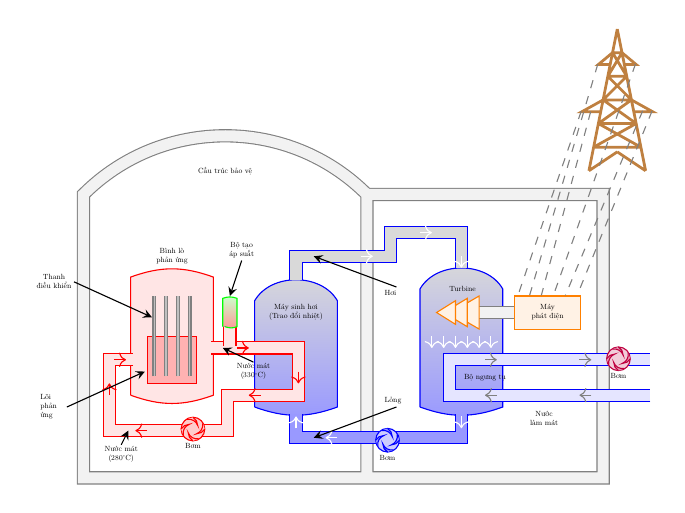
\begin{tikzpicture}[
            scale=0.3,
            annotline/.style = {stealth-},
            arrows1loop/.style={->,red},
            arrows2loop/.style={->,white},
            arrows3loop/.style={->,draw=gray},
            transform shape
        ]
    %Containment structure
    \draw[draw=gray,double=gray!10,double distance=4pt]
        (12,12) to[out=135,in=45](0,12)--(0,0)--(22,0)--(22,12)--(12,12)--(12,0);
    \node[text width=4cm, text centered,font=\small] at (6,13)
        {Cấu trúc bảo vệ};
    % % legend
    % \begin{scope}[yshift=-2cm]
    %     \filldraw[draw=red,fill=red!10] (1,0) rectangle ++(2,1);
    %     \node[text width=4cm, font=\small,right] at (3,0.5)
    %         {Nước áp lực\\(vòng sơ cấp)}; %Pressurized water (primary loop)
    %     \filldraw[draw=blue,bottom color=blue!40,top color=gray!30]
    %         (11,0) rectangle ++(2,1);
    %     \node[text width=4cm, font=\small,right] at (13,0.5)
    %         {Nước và hơi nước\\(vòng thứ cấp)}; %Water and steam\\(secondary loop)
    %     \filldraw[draw=blue,fill=blue!10] (21,0) rectangle ++(2,1);
    %     \node[text width=4cm, font=\small,right] at (23,0.5)
    %         {Nước làm mát\\(vòng giải nhiệt)}; %Water\\(cooling loop)
    % \end{scope}
    % 2nd loop --------------------------------------------------------------------
    \begin{scope}[xshift=7.25cm,yshift=3cm]
        % vessel left
        \filldraw[draw=blue,bottom color=blue!40,top color=gray!30]
            (0,0) to[out=-20,in=200] (3.5,0) --
            (3.5,4.5) to[out=120,in=60] (0,4.5) -- (0,0);
        % vessel right
        \filldraw[draw=blue,bottom color=blue!40,top color=gray!30,xshift=7cm]
            (0,0) to[out=-20,in=200] (3.5,0) --
            (3.5,5) to[out=120,in=60] (0,5) -- (0,0);
        % circuits
        \draw[draw=blue,double=blue!40,double distance=4pt]
        (1.75,-0.3) -- ++(0,-1) -- ++(7,0) -- ++(0,1);
        \draw[draw=blue,double=gray!30,double distance=4pt]
            (1.75,5.38) -- ++(0,1) -- ++(4,0) -- ++(0,1) -- ++(3,0) -- ++(0,-1.5);
        % arrows
        \draw[arrows2loop] (3.5,-1.3) -- (3,-1.3);
        \draw[arrows2loop] (1.75,-0.9) -- (1.75,-0.4);
        \draw[arrows2loop] (4.5,6.38) -- (5,6.38);
        \draw[arrows2loop] (7,7.38) -- (7.5,7.38);
        \draw[arrows2loop] (8.75,6.4) -- (8.75,5.9);
        \draw[arrows2loop] (8.75,-0.4) -- (8.75,-0.9);
        %
        \foreach \x in {0.5,1,...,3}
            \draw[arrows2loop,xshift=7cm] (\x,3) -- (\x,2.5);
        % labels
        \draw[annotline] (2.5,-1.3) -- ++(3.5,1.3)
            node[text width=1cm,font=\small,above] {Lỏng}; %Liquid
        \draw[annotline] (2.5,6.38) -- ++(3.5,-1.3)
            node[text width=1cm,font=\small,below] {Hơi};%Vapor
        % pump
        \begin{scope}[xshift=160,yshift=-40]
            \filldraw[fill=blue!20,draw=blue] (0,0) circle (0.5cm);
            \node[below,font=\small] at (0,-0.5) {Bơm}; %Pump
            \filldraw[fill=blue!40,draw=blue,yshift=-0.5cm]
                (0,0) arc (240:180:0.4cm)  arc (200:280:0.4cm) ;
            \filldraw[fill=blue!40,draw=blue,yshift=+0.5cm,rotate=180]
                (0,0) arc (240:180:0.4cm)  arc (200:280:0.4cm) ;
            \filldraw[fill=blue!40,draw=blue,xshift=+0.5cm,rotate=90]
                (0,0) arc (240:180:0.4cm)  arc (200:280:0.4cm) ;
            \filldraw[fill=blue!40,draw=blue,xshift=-0.5cm,rotate=-90]
                (0,0) arc (240:180:0.4cm)  arc (200:280:0.4cm) ;
        \end{scope}
        % generator ...
        \draw[xshift=6.5cm,draw=gray,double=gray!10,double distance=4pt] 
            (3,4) -- ++(2,0);
        \filldraw[xshift=6.5cm,fill=orange!10,draw=orange] 
            (1.8,4) -- (3.0,3.3) -- (3.0,4.7) -- cycle;
        \filldraw[xshift=6.5cm,fill=orange!10,draw=orange] 
            (1.5,4) -- (2.5,3.4) -- (2.5,4.6) -- cycle;
        \filldraw[xshift=6.5cm,fill=orange!10,draw=orange] 
            (1.2,4) -- (2  ,3.5) -- (2  ,4.5) -- cycle;
        \filldraw[xshift=6.5cm,fill=orange!10,draw=orange] 
            (4.5,3.3) rectangle (7.3,4.7);
        %labels
        \node[text width=3cm, text centered,font=\small] at (1.75,4) 
            {Máy sinh hơi\\(Trao đổi nhiệt)}; %Steam generator\\ (heat change)
        \node[text width=2cm, text centered,font=\small] at (8.8,5) {Turbine};
        \node[text width=2cm, text centered,font=\small] at (12.4,4) {Máy phát điện}; %Alternator
        % transmission lines
        \node (aa) at (11.1,4.6) {};
        \node (bb) at (11.6,4.6) {};
        \node (cc) at (12.1,4.6) {};
        \node (dd) at (12.6,4.6) {};
        \node (ee) at (13.1,4.6) {};
        \node (ff) at (13.6,4.6) {};

    \end{scope}
    % 3 loop --------------------------------------------------------------------
    \begin{scope}[xshift=23cm,yshift=1cm]
        % circuit
        \draw[draw=blue,double=blue!10,double distance=4pt]
        (1,2.5) -- ++(-8.5,0) -- ++(0,+1.5) -- ++(8.5,0);
        % arrows
        \draw[arrows3loop] (-5.5,2.5) -- (-6,2.5);
        \draw[arrows3loop] (-1.5,2.5) -- (-2,2.5);
        \draw[arrows3loop] (-6,4) -- (-5.5,4);
        \draw[arrows3loop] (-2,4) -- (-1.5,4);
        % % tower
        % \filldraw[draw=gray,fill=gray!20] (1,7) to[out=270,in=80]
        %             (0,0) to[out=-20,in=200]
        %             (6,0) to[out=100,in=270]
        %             (5,7);
        % \filldraw[draw=gray,fill=gray!40] (1,7) to[out=30,in=150]
        %             (5,7) to[out=200,in=-20]
        %             (1,7);
        % % labels
        % \node[text width=3cm, text centered,font=\small] at (3,3.5)
        %     {Tháp\\giải nhiệt};%Cooling\\tower
        \node[text width=2cm, text centered,font=\small] at (-3.5,1.5)
            {Nước\\làm mát};%Cooling\\water
        \node[text width=2cm, text centered,font=\small] at (-6,3.25)
            {Bộ ngưng tụ}; %Condenser
        % pump
        \begin{scope}[xshift=-10,yshift=115]
            \filldraw[fill=purple!20,draw=purple] (0,0) circle (0.5cm);
            \node[below,font=\small] at (0,-0.5) {Bơm};
            \filldraw[fill=purple!40,draw=purple,yshift=-0.5cm]
                (0,0) arc (240:180:0.4cm)  arc (200:280:0.4cm) ;
            \filldraw[fill=purple!40,draw=purple,yshift=+0.5cm,rotate=180]
                (0,0) arc (240:180:0.4cm)  arc (200:280:0.4cm) ;
            \filldraw[fill=purple!40,draw=purple,xshift=+0.5cm,rotate=90]
                (0,0) arc (240:180:0.4cm)  arc (200:280:0.4cm) ;
            \filldraw[fill=purple!40,draw=purple,xshift=-0.5cm,rotate=-90]
                (0,0) arc (240:180:0.4cm)  arc (200:280:0.4cm) ;
        \end{scope}
    \end{scope}
    %1 loop --------------------------------------------------------------------
    \begin{scope}[xshift=2cm,yshift=4cm]
    % Reactor vessel
    \filldraw[draw=red,fill=red!10] (0,-0.5) to[out=-20,in=200]
                (3.5,-0.5) --
                (3.5,4.5) to[out=160,in=20]
                (0,4.5) --
                (0,-0.5);
    % circuit
    \draw[draw=red,double=red!10,double distance=4pt]
    (0.1,1) --  ++(-1,0) -- ++(0,-3) -- ++(5,0) -- ++(0,1.5) --
    ++(3,0) -- ++(0,2) -- ++(-3.7,0);
    % Pressurizer
    \draw[draw=red,double=red!10,double distance=4pt] (4.2,1.6) -- ++(0,0.8);
    \filldraw[draw=green,bottom color=red!40,top color=green!20]
                (4,2.4) to[out=-20,in=200]
                (4.5,2.4) --
                (4.5,3.6) to[out=160,in=20]
                (3.9,3.6) --
                (3.9,2.4);
    % arrows
    \draw[arrows1loop] (-0.7,1) -- (-0.2,1);
    \draw[arrows1loop] (-0.9,-0.5) -- (-0.9,0);
    \draw[arrows1loop] (0.7,-2) -- (0.2,-2);
    \draw[arrows1loop] (4.5,1.5) -- (5,1.5);
    \draw[arrows1loop] (7.1,0.5) -- (7.1,0);
    \draw[arrows1loop] (5.5,-0.5) -- (5,-0.5);

    % pump
    \begin{scope}[xshift=75,yshift=-55,fill=red!20,draw=red]
        \filldraw (0,0) circle (0.5cm);
        \node[below,font=\small] at (0,-0.5) {Bơm};
        \filldraw[yshift=-0.5cm] (0,0) arc (240:180:0.4cm)  arc (200:280:0.4cm) ;
        \filldraw[yshift=+0.5cm,rotate=180]
            (0,0) arc (240:180:0.4cm)  arc (200:280:0.4cm) ;
        \filldraw[xshift=+0.5cm,rotate=90]
            (0,0) arc (240:180:0.4cm)  arc (200:280:0.4cm) ;
        \filldraw[xshift=-0.5cm,rotate=-90]
            (0,0) arc (240:180:0.4cm)  arc (200:280:0.4cm) ;
    \end{scope}
    % reactor core
    \filldraw[fill=red!30,draw=red] (0.7,0) rectangle (2.8,2);

    % control rods
    \foreach \x in {1.0,1.5,2.0,2.5}
    \draw[draw=gray,double=gray!50,double distance=0.5pt] (\x,0.3) -- (\x,3.7);

    %labels
    \draw[annotline] (0.6,0.5) -- ++(-3.3,-1.5)
        node[text width=1cm,font=\small,left] {Lõi phản ứng}; %Reactor core
    \node[text width=2cm, text centered,font=\small] at (1.75,5.4) {Bình lò phản ứng}; %Reactor vessel
    \draw[annotline] (0.9,2.8) -- ++(-3.3,1.5)
        node[text width=2cm, text centered,font=\small,left=-8pt] {Thanh điều khiển}; %Control\\rods
    \draw[annotline] (4.2,3.7) -- ++(0.5,1.5)
        node[text width=2cm, text centered,font=\small,above] {Bộ tạo áp suất}; %Pressurizer
    \draw[annotline] (3.9,1.5) -- ++(1.3,-0.6)
        node[text width=2.4cm, text centered,below=-2pt,font=\small]
            {Nước mát (${330 ^\circ \mathrm{C}}$)}; %Water coolant 
    \draw[annotline] (-0.1,-2) -- ++(-0.3,-0.6)
        node[text width=2.4cm, text centered,below=-2pt,font=\small]
            {Nước mát (${280 ^\circ \mathrm{C}}$)};
    \end{scope}
    % % clouds ----------------------------------
    % \begin{scope}[xshift=26cm,yshift=10cm, fill=blue!10, draw=blue,
    %     decoration={bumps,segment length=0.5cm}]
    %     \filldraw[yshift=-1.5cm,rotate=-25,decorate]
    %         (0,0) -- ++(-0.4,1.25)-- ++(-0.1,0.75)-- ++(0.2,0.5)-- ++(0.3,0.5)--
    %         ++(0.3,-0.5)-- ++(0.2,-0.5)-- ++(-0.1,-0.75)-- ++(-0.4,-1.25);
    %     \filldraw[xshift=0.5cm,yshift=-2cm,rotate=-30,decorate]
    %         (0,0) -- ++(-0.4,1.25)-- ++(-0.1,0.75)-- ++(0.2,0.5)-- ++(0.3,0.5)--
    %         ++(0.3,-0.5)-- ++(0.2,-0.5)-- ++(-0.1,-0.75)-- ++(-0.4,-1.25);
    %     \filldraw[xshift=-1.05cm,yshift=-2.15cm,rotate=-20,decorate]
    %         (0,0) -- ++(-0.4,1.25)-- ++(-0.1,0.75)-- ++(0.2,0.5)-- ++(0.3,0.5)--
    %         ++(0.3,-0.5)-- ++(0.2,-0.5)-- ++(-0.1,-0.75)-- ++(-0.4,-1.25);
    %     %labels
    %     \node[text width=1cm, text centered,font=\small] at (0.2,1.5) {Hơi nước};%Water vapor
    % \end{scope}

    % palo della luce
    \begin{scope}[xscale=0.2,xshift=113cm,yshift=19cm,line width=1pt,brown]
        \draw (0,0) -- (-6,-6)
            (0,0) -- ( 6,-6)
            (-1,-1) -- ( 1,-1)
            (-1,-1) -- ( 2,-2)
            ( 1,-1) -- (-2,-2)
            (-2,-2) -- ( 2,-2)
            (-2,-2) -- ( 3,-3)
            ( 2,-2) -- (-3,-3)
            ( 3,-3) -- (-3,-3)
            (-3,-3) -- ( 4,-4)
            ( 3,-3) -- (-4,-4)
            ( 4,-4) -- (-4,-4)
            (-4,-4) -- ( 5,-5)
            ( 4,-4) -- (-5,-5)
            ( 5,-5) -- (-5,-5)
            (-6,-6) -- ( 0,-5.2)
            ( 6,-6) -- ( 0,-5.2);
        \draw (-1.5,-1.5) -- (-4,-1.5) -- (-1,-1)
            ( 1.5,-1.5) -- ( 4,-1.5) -- ( 1,-1);
        \path (-4,-1.4) node (a) {}
            ( 4,-1.4) node (b) {};
        \draw[line width=1pt,brown] (-3.5,-3.5) -- (-7.5,-3.5) -- (-3,-3)
                                    ( 3.5,-3.5) -- ( 7.5,-3.5) -- ( 3,-3);
        \path (-7.5,-3.4) node (c) {}
            ( 7.5,-3.4) node (d) {}
            (-5.5,-3.4) node (e) {}
            ( 5.5,-3.4) node (f) {};
    \end{scope}
    % transmission lines
    \draw[dashed,gray] (c) -- (aa)
                    (a) -- (bb)
                    (e) -- (cc)
                    (b) -- (dd)
                    (f) -- (ee)
                    (d) -- (ff);
    \end{tikzpicture}
}
\choiceTF
{\True Lò phản ứng hạt nhân hoạt động dựa trên nguyên lý phản ứng phân hạch dây chuyền}
{Hiệu suất của nhà máy điện hạt nhân này là ${68\%}$}
{Biết $^{235}_{92}\mathrm{U}$ mất dần do phân hạch với tốc độ ${R}$ và nó cũng bị hao hụt do sự bắt neutron (mà không gây phân hạch) với tốc độ trung bình là ${\frac{1}{4}R}$. Với tốc độ tiêu thụ nhiên liệu như thế, nhà máy hoạt động trong ${570}$ ngày với khối lượng nhiên liệu như trên}
{\True Ưu điểm vượt trội của năng lượng hạt nhân so với năng lượng hóa thạch là cắt giảm lượng khí thải gây ô nhiễm vào bầu khí quyển Trái đất. Nhà máy điện hạt nhân giải quyết được vấn đề thiếu hụt về năng lượng khi nguồn năng lượng hóa thạch đang dần cạn kiệt}
\loigiai{
\begin{itemchoice}
\itemch 
\itemch ${H = \frac{P_d}{P_n} = \frac{1100}{3400} \approx 0{,}32 = 32\%}$.
\itemch ${n_U = \frac{m_U}{M} = \frac{\frac{2{,}98}{100} \cdot 86000}{0{,}235} \approx 10905{,}532 \, \mathrm{mol}}$.\\
${N_U = n_U N_A = 10905{,}532 \cdot 6{,}02 \cdot 10^{23} \approx 6{,}57 \cdot 10^{27}}$.\\
${R = \frac{P_{nh}}{\Delta E} = \frac{3400 \cdot 10^6}{2 \cdot 10^2 \cdot 1{,}6 \cdot 10^{-13}} = 1{,}0625 \cdot 10^{20}}$ phân hạch/s.\\
${t = \frac{N_U}{R + \dfrac{R}{4}} = \frac{6{,}57 \cdot 10^{27}}{\dfrac{5}{4} \cdot 1{,}0625 \cdot 10^{20}} \, \mathrm{giây} > 570 \, \mathrm{ngày}}$.
\itemch Nhà máy điện hạt nhân không thải ${\mathrm{CO_2}}$ như hóa thạch.
\end{itemchoice}
}
\end{ex}


% Câu 1
\begin{ex}
Khi tổng hợp hạt nhân $^4_2\mathrm{He}$ từ phản ứng hạt nhân $^1_1\mathrm{H} + ^7_3\mathrm{Li} \to ^4_2\mathrm{He} + \mathrm{X}$ mỗi phản ứng trên toả năng lượng ${17{,}3 \, \mathrm{MeV}}$. Năng lượng toả ra khi tổng hợp được ${0{,}5 \, \mathrm{mol}}$ helium bằng ${z \cdot 10^{24} \, \mathrm{MeV}}$. Giá trị ${z}$ bằng bao nhiêu (làm tròn kết quả đến chữ số hàng phần mười)?
\shortans{2{,}6}
\loigiai{
$^1_1\mathrm{H} + ^7_3\mathrm{Li} \to ^4_2\mathrm{He} + ^4_2\mathrm{He}$.\\
${N_{\mathrm{He}} = n_{\mathrm{He}} N_A = 0{,}5 \cdot 6{,}02 \cdot 10^{23} = 3{,}01 \cdot 10^{23}}$.\\
${N = \frac{N_{\mathrm{He}}}{2} = \frac{3{,}01 \cdot 10^{23}}{2} = 1{,}505 \cdot 10^{23}}$.\\
${Q = N \Delta E = 1{,}505 \cdot 10^{23} \cdot 17{,}3 \approx 2{,}6 \cdot 10^{24} \, \mathrm{MeV}}$.
}
\end{ex}


% Câu 2
\begin{ex}
Một nhà máy điện hạt nhân tiêu thụ trung bình ${58{,}75 \, \mathrm{g}} \, ^{235}_{92}\mathrm{U}$ mỗi ngày. Giả thiết sau mỗi phân hạch trung bình có ${2{,}5}$ neutron được giải phóng thì sau một ngày số neutron thu được trong lò phản ứng là ${X \cdot 10^{23}}$. Giá trị của ${X}$ bằng bao nhiêu (làm tròn kết quả đến chữ số hàng phần trăm)? Cho rằng neutron chỉ mất đi do bị hấp thụ bởi các $^{235}_{92}\mathrm{U}$ trong chuỗi phân hạch dây chuyền.
\shortans{2{,}26}
\loigiai{
${n = \frac{m}{M} = \frac{58{,}75}{235} = 0{,}25 \, \mathrm{mol}}$.\\
${N_U = n N_A = 0{,}25 \cdot 6{,}02 \cdot 10^{23} = 1{,}505 \cdot 10^{23}}$.\\
Mỗi phân hạch cần ${1}$ neutron và giải phóng ${2{,}5}$ neutron nên dư ra ${1{,}5}$ neutron.\\
${N_n = 1{,}5 N_U = 1{,}5 \cdot 1{,}505 \cdot 10^{23} \approx 2{,}26 \cdot 10^{23}}$.
}
\end{ex}


% Câu 3
\begin{ex}
Xét phản ứng nhiệt hạch: $^2_1\mathrm{H} + ^2_1\mathrm{H} \to ^4_2\mathrm{He}$ có năng lượng toả ra là ${3{,}25 \, \mathrm{MeV}}$. Nếu quá trình nhiệt hạch sử dụng hết ${150 \, \mathrm{g}} \, ^2_1\mathrm{H}$ thì tổng năng lượng thu được là ${z \cdot 10^{25} \, \mathrm{MeV}}$. Coi khối lượng mol tính theo gam bằng số khối của hạt nhân đó. Giá trị ${z}$ bằng bao nhiêu (làm tròn kết quả đến chữ số hàng phần trăm)?
\shortans{7{,}34}
\loigiai{
${n = \frac{m}{M} = \frac{150}{2} = 75 \, \mathrm{mol}}$.\\
${N_{\mathrm{H}} = n_{\mathrm{H}} N_A = 75 \cdot 6{,}02 \cdot 10^{23} = 4{,}515 \cdot 10^{25}}$.\\
${N = \frac{N_{\mathrm{H}}}{2} = \frac{4{,}515 \cdot 10^{25}}{2} = 2{,}2575 \cdot 10^{25}}$.\\
${Q = N \Delta E = 2{,}2575 \cdot 10^{25} \cdot 3{,}25 \approx 7{,}34 \cdot 10^{25} \, \mathrm{MeV}}$.
}
\end{ex}


% Câu 4
\begin{ex}
Giả sử quả bom nguyên tử thả xuống Hiroshima có chứa ${100 \, \mathrm{kg}}$ quặng uranium trong đó $^{235}_{92}\mathrm{U}$ chiếm ${25\%}$. Lấy khối lượng ${1 \, \mathrm{mol}} \, ^{235}_{92}\mathrm{U}$ bằng ${235 \, \mathrm{g/mol}}$. Nếu trung bình mỗi phân hạch của $^{235}_{92}\mathrm{U}$ giải phóng ${200 \, \mathrm{MeV}}$ thì năng lượng giải phóng của vụ nổ tương đương bao ${z \cdot 10^8}$ số điện (${1}$ số điện $= {1 \, \mathrm{kWh}}$). Giá trị ${z}$ bằng bao nhiêu (làm tròn kết quả đến chữ số hàng phần mười)?
\shortans{5{,}7}
\loigiai{
${n = \frac{m}{M} = \frac{25 \cdot 10^3}{235} = \frac{5000}{47} \, \mathrm{mol}}$.\\
${Q = N \Delta E = n N_A \Delta E = \frac{5000}{47} \cdot 6{,}02 \cdot 10^{23} \cdot 200 \cdot 1{,}6 \cdot 10^{-13} = 2{,}05 \cdot 10^{15} \, \mathrm{J} \approx 5{,}7 \cdot 10^8 \, \mathrm{kWh}}$.
}
\end{ex}


% Câu 5-6
\begin{ex}
\sochc{2}{Bom hydrogen (bom H) là một loại vũ khí hạt nhân có sức tàn phá lớn hơn bom nguyên tử (bom A) rất nhiều lần, dù hiện nay cả bom hydrogen và bom nguyên tử đều không được sử dụng trong các cuộc chiến tranh. Sở dĩ bom hydrogen có sức tàn phá lớn như vậy là do nó là sự kết hợp của phản ứng phân hạch của $^{235}_{92}\mathrm{U}$ (giai đoạn ${1}$) để tạo ra môi trường có nhiệt độ rất cao, cung cấp động năng cho các hạt tham gia phản ứng nhiệt hạch (giai đoạn ${2}$) theo phương trình phản ứng $^2_1\mathrm{H} + ^3_1\mathrm{H} \to ^4_2\mathrm{He} + ^1_0\mathrm{n} + {17{,}6 \, \mathrm{MeV}}$. Giả sử năng lượng toả ra từ quá trình phân hạch còn lại sau khi tạo phản ứng nhiệt hạch là ${2{,}8 \cdot 10^{10} \, \mathrm{J}}$ và khối lượng $^4_2\mathrm{He}$ được tạo thành từ một vụ nổ bom hydrogen trong thí nghiệm vũ khí hạt nhân là ${200 \, \mathrm{g}}$.
}
\begin{chc}
Khối lượng mol của $^4_2\mathrm{He}$ là ${4 \, \mathrm{g/mol}}$. Tổng năng lượng tỏa ra của các phản ứng nhiệt hạch sau khi bom nổ là ${z \cdot 10^{13} \, \mathrm{J}}$. Giá trị ${z}$ bằng bao nhiêu (làm tròn kết quả đến chữ số hàng phần mười)?
\shortans{8{,}5}
\loigiai{
${n = \frac{m}{M} = \frac{200}{4} = 50 \, \mathrm{mol}}$.\\
${N = n N_A = 50 \cdot 6{,}02 \cdot 10^{23} = 3{,}01 \cdot 10^{25}}$.\\
${Q_2 = N \Delta E_2 = 3{,}01 \cdot 10^{25} \cdot 17{,}6 \cdot 1{,}6 \cdot 10^{-13} \approx 8{,}5 \cdot 10^{13} \, \mathrm{J}}$.
}
\end{chc}
\begin{chc}
Biết rằng năng lượng toả ra khi một tấn thuốc nổ TNT cháy hoàn toàn là ${4{,}2 \cdot 10^9 \, \mathrm{J}}$. Sức tàn phá của quả bom này tương đương với ${z \cdot 10^3}$ tấn thuốc nổ TNT. Giá trị ${z}$ bằng bao nhiêu (làm tròn kết quả đến chữ số hàng phần mười)?
\shortans{20{,}2}
\loigiai{
${m = \frac{Q_1 + Q_2}{4{,}2 \cdot 10^9} = \frac{2{,}8 \cdot 10^{10} + 8{,}5 \cdot 10^{13}}{4{,}2 \cdot 10^9} \approx 20{,}2 \cdot 10^3}$ tấn.
}
\end{chc}
\end{ex}

% Câu 1
\begin{ex}
    Lực hạt nhân giữa các nucleon trong hạt nhân là
    \choice
    {lực điện}
    {\True lực hút}
    {lực đẩy}
    {lực từ}
    \loigiai{Lực hạt nhân là lực hút giữa các nucleon.}
\end{ex}


% Câu 2
\begin{ex}
    Đơn vị nào sau đây là đơn vị cơ bản trong hệ SI?
    \choice
    {\True ${K}$}
    {${Hz}$}
    {${N}$}
    {${^\circ\mathrm{C}}$}
    \loigiai{Trong hệ SI, Kelvin (${K}$) là đơn vị cơ bản của nhiệt độ nhiệt động lực học.}
\end{ex}


% Câu 3
\begin{ex}
    Hạt nhân nguyên tử nào sau đây là đồng vị của hạt nhân nguyên tử ${^A_Z X}$?
    \choice
    {${^A_{Z-1} X}$}
    {\True ${^{A+1}_Z X}$}
    {${^{A-1}_{Z-1} X}$}
    {${^A_{Z+1} X}$}
    \loigiai{Đồng vị là những hạt nhân có cùng số proton ${Z}$ nhưng khác số neutron ${N}$.}
\end{ex}


% Câu 4
\begin{ex}
    Năng lượng bức xạ mặt trời chủ yếu đến từ ... bên trong mặt trời. Chỗ trống là
    \choice
    {phản ứng hóa học}
    {\True phản ứng nhiệt hạch}
    {phản ứng phân hạch}
    {phản ứng phóng xạ}
    \loigiai{Năng lượng mặt trời chủ yếu do phản ứng nhiệt hạch (tổng hợp hạt nhân) xảy ra ở tâm mặt trời.}
\end{ex}


% Câu 5
\begin{ex}
    Hai khối nhôm ${A}$ và ${B}$ có cùng nhiệt độ ban đầu. Khối lượng của ${A}$ gấp ba lần khối lượng của ${B}$. Sau khi chúng tỏa ra cùng một lượng nhiệt thì cho chúng tiếp xúc với nhau, ta thấy
    \choice
    {\True ${A}$ truyền nhiệt cho ${B}$}
    {${B}$ truyền nhiệt cho ${A}$}
    {nhiệt độ được truyền từ ${B}$ sang ${A}$}
    {nhiệt độ được truyền từ ${A}$ sang ${B}$}
    \loigiai{Ta có ${Q = mc\Delta t \Rightarrow \Delta t = \frac{Q}{mc}}$. Vì ${m_A = 3m_B}$ và cùng tỏa ra nhiệt lượng ${Q}$ nên ${\Delta t_A = \frac{1}{3} \Delta t_B}$. Do đó nhiệt độ của ${A}$ giảm ít hơn ${B}$, dẫn đến ${T_A > T_B}$. Khi tiếp xúc, nhiệt truyền từ vật có nhiệt độ cao sang vật có nhiệt độ thấp, tức là từ ${A}$ sang ${B}$.}
\end{ex}


% Câu 6
\begin{ex}
    Trong các cuộc thi đấu môn bi đá trên băng, các vận động viên sử dụng chổi liên tục chà sát bề mặt băng để tạo thành một lớp màng nước trên bề mặt băng và giảm ma sát giữa bi đá và bề mặt băng. Sự hình thành lớp nước trên bề mặt băng là hiện tượng
    \choice
    {\True nóng chảy}
    {đông đặc}
    {thăng hoa}
    {ngưng tụ}
    \loigiai{Sự chuyển từ thể rắn (băng) sang thể lỏng (nước) là hiện tượng nóng chảy.}
\end{ex}


% Câu 7
\begin{ex}
    Chọn phát biểu đúng khi nói về từ trường?
    \choice
    {Tính chất cơ bản của từ trường là tác dụng lực từ lên các điện tích đặt trong nó}
    {\True Qua mỗi điểm trong từ trường chỉ vẽ được một và chỉ một đường sức từ}
    {Các đường sức từ luôn cắt nhau}
    {Các đường sức từ là những đường cong không khép kín}
    \loigiai{Theo định nghĩa về đường sức từ, qua mỗi điểm trong không gian có từ trường chỉ có thể vẽ được một đường sức từ duy nhất.}
\end{ex}


% Câu 8
\begin{ex}
    Rutherford đã sử dụng hạt alpha để bắn phá lá vàng mỏng nhằm nghiên cứu cấu trúc nguyên tử. Các kết quả thực nghiệm mà ông thu được là
    \choice
    {Tất cả các hạt alpha đều đi qua lá vàng mà không bị lệch hướng}
    {Hầu hết các hạt alpha bị tán xạ với góc lệch lớn}
    {Số lượng các hạt alpha tán xạ theo các hướng gần như bằng nhau}
    {\True Một lượng rất nhỏ các hạt alpha bị tán xạ với góc lệch lớn hơn ${90^\circ}$}
    \loigiai{Trong thí nghiệm của Rutherford, hầu hết các hạt alpha đi thẳng, một số ít bị lệch hướng và một lượng rất nhỏ bị bật ngược trở lại (góc lệch lớn hơn ${90^\circ}$).}
\end{ex}


% Câu 9
\begin{ex}
    Một lượng khí lí tưởng nhất định có nhiệt độ không thay đổi. Khi thể tích của khí là ${V}$ thì áp suất là ${p}$. Khi thể tích của khí là ${2V}$ thì áp suất là
    \choice
    {${2p}$}
    {\True ${\frac{1}{2}p}$}
    {${4p}$}
    {${\frac{1}{4}p}$}
    \loigiai{Theo định luật Boyle-Mariotte, đối với một lượng khí lí tưởng xác định ở nhiệt độ không đổi, áp suất tỉ lệ nghịch với thể tích: ${p_1 V_1 = p_2 V_2 \Rightarrow p \cdot V = p_2 \cdot 2V \Rightarrow p_2 = \frac{1}{2}p}$.}
\end{ex}


% Câu 10
\begin{ex}
    Trong các hạt nhân ${^{206}_{82} \mathrm{Pb}}$; ${^{226}_{88} \mathrm{Ra}}$; ${^{210}_{84} \mathrm{Po}}$; ${^{238}_{92} \mathrm{U}}$ hạt nhân có nhiều neutron nhất là?
    \choice
    {\True ${^{238}_{92} \mathrm{U}}$}
    {${^{226}_{88} \mathrm{Ra}}$}
    {${^{210}_{84} \mathrm{Po}}$}
    {${^{206}_{82} \mathrm{Pb}}$}
    \loigiai{Số neutron ${N = A - Z}$.\\
    ${N_{\mathrm{Pb}} = 206 - 82 = 124}$\\
    ${N_{\mathrm{Ra}} = 226 - 88 = 138}$\\
    ${N_{\mathrm{Po}} = 210 - 84 = 126}$\\
    ${N_{\mathrm{U}} = 238 - 92 = 146}$\\
    Vậy hạt nhân ${^{238}_{92} \mathrm{U}}$ có nhiều neutron nhất.}
\end{ex}


% Câu 11
\begin{ex}
    Một dòng điện có cường độ ${i = 2\cos\left(100\pi t + \frac{\pi}{6}\right) \, \mathrm{(A)}}$. Tần số của dòng điện này bằng
    \choice
    {\True ${50 \, \mathrm{Hz}}$}
    {${100 \, \mathrm{Hz}}$}
    {${\sqrt{2} \, \mathrm{Hz}}$}
    {${100\sqrt{2} \, \mathrm{Hz}}$}
    \loigiai{Tần số của dòng điện là ${f = \frac{\omega}{2\pi} = \frac{100\pi}{2\pi} = 50 \, \mathrm{Hz}}$.}
\end{ex}


% Câu 12
\begin{ex}
    Truyền nhiệt lượng ${390 \, \mathrm{J}}$ cho ${150 \, \mathrm{g}}$ chì thì nhiệt độ tăng từ ${15^\circ\mathrm{C}}$ đến ${35^\circ\mathrm{C}}$. Nhiệt dung riêng của chì là
    \choice
    {${260 \, \mathrm{J/(kg \cdot K)}}$}
    {\True ${130 \, \mathrm{J/(kg \cdot K)}}$}
    {${390 \, \mathrm{J/(kg \cdot K)}}$}
    {${520 \, \mathrm{J/(kg \cdot K)}}$}
    \loigiai{Ta có ${Q = mc\Delta t \Rightarrow 390 = 0{,}15 \cdot c \cdot (35 - 15) \Rightarrow c = 130 \, \mathrm{J/(kg \cdot K)}}$.}
\end{ex}


% Câu 13
\begin{ex}
    Trong thời gian ${\Delta t}$, từ thông qua một mạch kín tăng đều một lượng bằng ${2 \, \mathrm{Wb}}$ và suất điện động cảm ứng xuất hiện trong mạch trong khoảng thời gian này có độ lớn ${8 \, \mathrm{V}}$. Giá trị của ${\Delta t}$ bằng
    \choice
    {${0{,}75 \, \mathrm{s}}$}
    {${1 \, \mathrm{s}}$}
    {${0{,}5 \, \mathrm{s}}$}
    {\True ${0{,}25 \, \mathrm{s}}$}
    \loigiai{Độ lớn suất điện động cảm ứng: ${e = \left| \frac{\Delta \Phi}{\Delta t} \right| \Rightarrow 8 = \frac{2}{\Delta t} \Rightarrow \Delta t = 0{,}25 \, \mathrm{s}}$.}
\end{ex}


% Câu 14
\begin{ex}
    Một khối khí lí tưởng ở nhiệt độ ${27^\circ\mathrm{C}}$ có áp suất ${3 \cdot 10^{-9} \, \mathrm{Pa}}$. Mật độ phân tử khí của khối khí này là
    \choice
    {${5 \cdot 10^{10} \, \mathrm{phân\, tử/cm^3}}$}
    {\True ${7{,}2 \cdot 10^5 \, \mathrm{phân\, tử/cm^3}}$}
    {${2{,}7 \cdot 10^8 \, \mathrm{phân\, tử/cm^3}}$}
    {${7{,}2 \cdot 10^{11} \, \mathrm{phân\, tử/cm^3}}$}
    \loigiai{Ta có ${p = \mu kT \Rightarrow 3 \cdot 10^{-9} = \mu \cdot 1{,}38 \cdot 10^{-23} \cdot (27 + 273) \Rightarrow \mu \approx 7{,}2 \cdot 10^{11} \, \mathrm{m^{-3}} = 7{,}2 \cdot 10^5 \, \mathrm{cm^{-3}}}$.}
\end{ex}


% Câu 15
\begin{ex}
    Một đoạn dây dẫn thẳng dài ${6 \, \mathrm{cm}}$ có cường độ dòng điện ${5 \, \mathrm{A}}$ chạy qua đặt trong từ trường đều có cảm ứng từ ${0{,}5 \, \mathrm{T}}$. Lực từ tác dụng lên đoạn dây có độ lớn ${75 \, \mathrm{mN}}$. Góc hợp bởi dây dẫn và đường sức từ là
    \choice
    {${45^\circ}$}
    {\True ${30^\circ}$}
    {${60^\circ}$}
    {${90^\circ}$}
    \loigiai{Lực từ tác dụng lên đoạn dây: ${F = ILB \sin \alpha \Rightarrow 75 \cdot 10^{-3} = 5 \cdot 0{,}06 \cdot 0{,}5 \cdot \sin \alpha \Rightarrow \sin \alpha = 0{,}5 \Rightarrow \alpha = 30^\circ}$.}
\end{ex}


% Câu 16
\begin{ex}
    Một piston nhẹ bịt kín một lượng khối khí lí tưởng trong xilanh đặt thẳng đứng. Ban đầu khối khí có thể tích 4 lít, nhiệt độ ${250 \, \mathrm{K}}$ và áp suất ${10^5 \, \mathrm{Pa}}$. Đẩy piston một đoạn để nén khí thì nhiệt độ và áp suất của khí thu được lần lượt là ${300 \, \mathrm{K}}$ và ${1{,}6 \cdot 10^5 \, \mathrm{Pa}}$. Thể tích khí lúc này là
    \choice
    {${2{,}0 \, \mathrm{lít}}$}
    {\True ${3{,}0 \, \mathrm{lít}}$}
    {${1{,}5 \, \mathrm{lít}}$}
    {${2{,}5 \, \mathrm{lít}}$}
    \loigiai{Áp dụng phương trình trạng thái khí lí tưởng: ${\frac{p_1 V_1}{T_1} = \frac{p_2 V_2}{T_2} \Rightarrow \frac{10^5 \cdot 4}{250} = \frac{1{,}6 \cdot 10^5 \cdot V_2}{300} \Rightarrow V_2 = 3 \, \mathrm{lít}}$.}
\end{ex}


% Câu 17
\begin{ex}
    Cho biết khối lượng của proton, neutron và hạt nhân ${^4_2 \mathrm{He}}$ lần lượt là ${1{,}6726 \cdot 10^{-27} \, \mathrm{kg}}$; ${1{,}6749 \cdot 10^{-27} \, \mathrm{kg}}$ và ${6{,}6467 \cdot 10^{-27} \, \mathrm{kg}}$. Lấy ${c = 3 \cdot 10^8 \, \mathrm{m/s}}$. Năng lượng liên kết của ${^4_2 \mathrm{He}}$ là
    \choice
    {\True ${4{,}35 \cdot 10^{-12} \, \mathrm{J}}$}
    {${1{,}45 \cdot 10^{-20} \, \mathrm{J}}$}
    {${45 \, \mathrm{MeV}}$}
    {${25 \, \mathrm{MeV}}$}
    \loigiai{Độ hụt khối: ${\Delta m = Zm_p + (A-Z)m_n - m = 2 \cdot 1{,}6726 \cdot 10^{-27} + (4-2) \cdot 1{,}6749 \cdot 10^{-27} - 6{,}6467 \cdot 10^{-27}}$ \\
    ${\Rightarrow \Delta m = 0{,}0483 \cdot 10^{-27} \, \mathrm{kg}}$.\\
    Năng lượng liên kết: ${W_{lk} = \Delta m c^2 = 0{,}0483 \cdot 10^{-27} \cdot (3 \cdot 10^8)^2 \approx 4{,}35 \cdot 10^{-12} \, \mathrm{J}}$.}
\end{ex}


% Câu 18
\begin{ex}
    Mở vòi nước lạnh và vòi nước nóng để cùng đưa nước vào bồn tắm. Nhiệt độ của nước từ vòi nước lạnh là ${15^\circ\mathrm{C}}$ và từ vòi nước nóng là ${60^\circ\mathrm{C}}$. Cuối cùng trong bồn tắm có 150 lít nước ở nhiệt độ ${42^\circ\mathrm{C}}$. Bỏ qua sự trao đổi nhiệt với môi trường. Lượng nước thoát ra từ vòi nước lạnh và vòi nước nóng lần lượt là
    \choice
    {\True 60 lít và 90 lít}
    {90 lít và 60 lít}
    {30 lít và 120 lít}
    {120 lít và 30 lít}
    \loigiai{Gọi ${V_l, V_n}$ lần lượt là thể tích nước lạnh và nước nóng.\\
    Ta có hệ phương trình:
    ${\left\{\begin{aligned} V_l + V_n &= 150 \\ V_l \cdot 15 + V_n \cdot 60 &= 150 \cdot 42 \end{aligned}\right. \Rightarrow \left\{\begin{aligned} V_l &= 60 \, \mathrm{lít} \\ V_n &= 90 \, \mathrm{lít} \end{aligned}\right.}$.}
    \end{ex}
    
    
% Câu 1
\begin{ex}
    \immini[thm]{
        Một khối khí lí tưởng nhất định thực hiện quá trình biến đổi trạng thái ${A \to B \to C \to A}$ như trên đồ thị nhiệt độ nhiệt độ ${T}$ - thể tích ${V}$ hình bên. Biết áp suất của khí ở trạng thái ${C}$ là ${p_0}$.
        \choiceTF
        {Áp suất của khí ở trạng thái ${B}$ là ${2p_0}$}
        {\True Nhiệt độ của khí ở trạng thái ${A}$ là ${\frac{1}{2} T_0}$}
        {\True Trong quá trình ${B \to C}$, khí hấp thụ nhiệt}
        {Trong quá trình ${A \to B}$, khí thực hiện công ${p_0 V_0}$}
    }{
        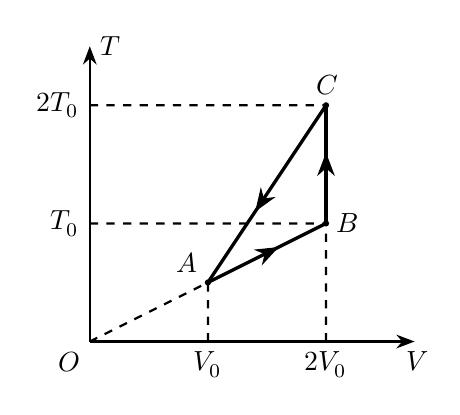
\begin{tikzpicture}[>={Stealth}, scale=0.75, thick]
            % --- Tọa độ các điểm chính ---
            % Giả sử: V0 = 2 đơn vị, T0 = 2 đơn vị
            % Điểm B ở (2V0, T0) => (4, 2)
            % Điểm C ở (2V0, 2T0) => (4, 4)
            % Điểm A ở (V0, T0/2) => (2, 1) vì A nằm trên đường thẳng đi qua gốc O và B
            \coordinate (O) at (0,0);
            \coordinate (A) at (2,1);
            \coordinate (B) at (4,2);
            \coordinate (C) at (4,4);

            % --- Vẽ hệ trục tọa độ ---
            \draw[->, thick] (0,0) -- (5.5,0) node[below] {$V$};
            \draw[->, thick] (0,0) -- (0,5) node[right] {$T$};
            \node[below left] at (O) {$O$};

            % --- Vẽ các đường dóng nét đứt và nhãn trục ---
            % Trục hoành (V)
            \draw[dashed] (2,0) node[below, black] {$V_0$} -- (A);
            \draw[dashed] (4,0) node[below, black] {$2V_0$} -- (B);
            
            % Trục tung (T)
            \draw[dashed] (0,2) node[left, black] {$T_0$} -- (B);
            \draw[dashed] (0,4) node[left, black] {$2T_0$} -- (C);
            
            % Đường nối từ gốc tọa độ đến điểm A (định hướng quá trình đẳng áp)
            \draw[dashed] (O) -- (A);

            % --- Vẽ các quá trình biến đổi có mũi tên chỉ hướng ---
            \begin{scope}[very thick, decoration={
                markings,
                mark=at position 0.6 with {\arrow{>}}}
                ]
                \draw[postaction={decorate}] (A) -- (B);
                \draw[postaction={decorate}] (B) -- (C);
                \draw[postaction={decorate}] (C) -- (A);
            \end{scope}

            % --- Vẽ các điểm nút và nhãn tên điểm ---
            \fill (A) circle (1.5pt) node[above left] {$A$};
            \fill (B) circle (1.5pt) node[right] {$B$};
            \fill (C) circle (1.5pt) node[above] {$C$};

        \end{tikzpicture}
    }
    \loigiai{
        \begin{itemchoice}
            \itemch ${BC}$ là quá trình đẳng tích: ${\frac{p_B}{T_B} = \frac{p_C}{T_C} \Rightarrow \frac{p_B}{T_0} = \frac{p_0}{2T_0} \Rightarrow p_B = \frac{p_0}{2}}$.
            \itemch ${AB}$ là quá trình đẳng áp: ${\frac{V_A}{T_A} = \frac{V_B}{T_B} \Rightarrow \frac{V_0}{T_A} = \frac{2V_0}{T_0} \Rightarrow T_A = \frac{T_0}{2}}$.
            \itemch Trong quá trình đẳng tích ${B \to C}$, công ${A = 0}$. Nhiệt độ tăng từ ${T_0}$ lên ${2T_0}$ nên nội năng tăng. Theo định luật I nhiệt động lực học: ${Q = \Delta U + A > 0}$, khí hấp thụ nhiệt.
            \itemch Công khí thực hiện trong quá trình đẳng áp ${A \to B}$: ${A' = p_B(V_B - V_A) = \frac{p_0}{2}(2V_0 - V_0) = \frac{p_0 V_0}{2}}$.
        \end{itemchoice}
        }
    \end{ex}
        
        
% Câu 2
\begin{ex}
    \immini[thm]{
        Hình bên là đồ thị biểu diễn mối quan hệ giữa áp suất ${p}$ và thể tích ${V}$ của một lượng khí lí tưởng nhất định. Khí trải qua quá trình biến đổi trạng thái ${A \to B \to C}$. Biết nhiệt độ của khí ở trạng thái ${A}$, ${B}$ và ${C}$ lần lượt là ${T_A, T_B}$ và ${T_C}$.
        \choiceTF
        {${4T_A = 3T_B}$}
        {\True ${15T_A = 4T_C}$}
        {Nhiệt độ của khí giảm dần trong quá trình ${A \to B}$}
        {\True Nhiệt độ của khí tăng dần trong quá trình ${B \to C}$}
    }{
        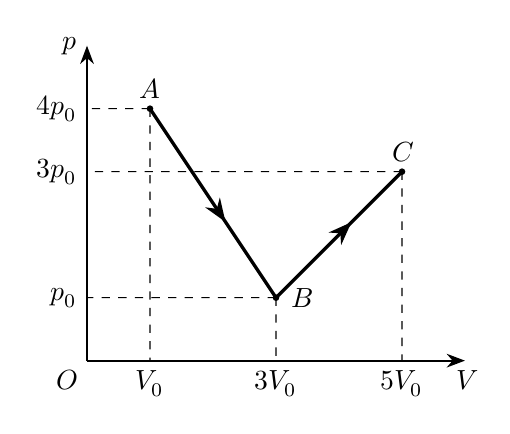
\begin{tikzpicture}[>={Stealth}, scale=0.8]
            % --- Tọa độ các điểm ---
            \coordinate (O) at (0,0);
            \coordinate (A) at (1,4);
            \coordinate (B) at (3,1);
            \coordinate (C) at (5,3);
    
            % --- Hệ trục tọa độ ---
            \draw[->, thick] (0,0) -- (6,0) node[below] {$V$};
            \draw[->, thick] (0,0) -- (0,5) node[left] {$p$};
            \node[below left] at (O) {$O$};
    
            % --- Đường dóng nét đứt ---
            % Điểm A
            \draw[dashed] (A) -- (1,0) node[below, black] {$V_0$};
            \draw[dashed] (A) -- (0,4) node[left, black] {$4p_0$};
            
            % Điểm B
            \draw[dashed] (B) -- (3,0) node[below, black] {$3V_0$};
            \draw[dashed] (B) -- (0,1) node[left, black] {$p_0$};
            
            % Điểm C
            \draw[dashed] (C) -- (5,0) node[below, black] {$5V_0$};
            \draw[dashed] (C) -- (0,3) node[left, black] {$3p_0$};
    
            % --- Quá trình biến đổi (Đã sửa lỗi 'with' và xóa \Large) ---
            \begin{scope}[very thick, decoration={
                markings,
                mark=at position 0.6 with {\arrow{>}}}
                ]
                \draw[postaction={decorate}] (A) -- (B);
                \draw[postaction={decorate}] (B) -- (C);
            \end{scope}
    
            % --- Điểm nút và nhãn tên ---
            \fill (A) circle (1.5pt) node[above] {$A$};
            \fill (B) circle (1.5pt) node[right=2pt] {$B$};
            \fill (C) circle (1.5pt) node[above] {$C$};
    
        \end{tikzpicture}
    }
    \loigiai{
        \begin{itemchoice}
        \itemch Áp dụng phương trình trạng thái: ${\frac{p_A V_A}{T_A} = \frac{p_B V_B}{T_B} \Rightarrow \frac{4p_0 V_0}{T_A} = \frac{p_0 \cdot 3V_0}{T_B} \Rightarrow 4T_B = 3T_A}$.
        \itemch Áp dụng phương trình trạng thái: ${\frac{p_A V_A}{T_A} = \frac{p_C V_C}{T_C} \Rightarrow \frac{4p_0 V_0}{T_A} = \frac{3p_0 \cdot 5V_0}{T_C} \Rightarrow 15T_A = 4T_C}$.
        \itemch Trong quá trình ${A \to B}$, tích ${pV}$ ban đầu là ${4p_0 V_0}$, tại ${B}$ là ${3p_0 V_0}$. Tuy nhiên trên đoạn thẳng ${AB}$, tích ${pV}$ có thể đạt giá trị cực đại lớn hơn ${4p_0 V_0}$ rồi mới giảm, nên nhiệt độ tăng rồi giảm.
        \itemch Trong quá trình ${B \to C}$, cả ${p}$ và ${V}$ đều tăng nên tích ${pV}$ tăng, dẫn đến nhiệt độ tăng dần.
        \end{itemchoice}
    }
\end{ex}


% Câu 3
\begin{ex}
\immini[thm]{
        Như hình vẽ, một đoạn dây dẫn thẳng khối lượng ${m}$ và dài ${l}$ được đặt trên một mặt phẳng nghiêng có góc nghiêng ${\theta}$ so với mặt phẳng ngang. Một từ trường đều có phương thẳng đứng hướng xuống có độ lớn cảm ứng từ là ${B}$. Bây giờ, cho dòng điện qua đoạn dây dẫn có chiều hướng ra ngoài trang giấy và cường độ ${i}$ tăng dần từ ${0}$ tới giá trị ${I}$ để đoạn dây bắt đầu trượt. Biết lực ma sát nghỉ cực đại bằng lực ma sát trượt và gia tốc rơi tự do là ${g}$.
    }{
        \begin{tikzpicture}[>=Stealth, scale=0.75, thick]
            % --- Thông số cơ bản ---
            \def\angle{25} % Góc nghiêng theta
            \def\L{5.5}    % Chiều dài cạnh huyền
            \def\r{0.25}   % Bán kính vòng dây (dòng điện i)

            % --- Vẽ từ trường B (các mũi tên màu xám hướng xuống) ---
            \foreach \x in {0.5, 2, 3.5, 5} {
                \draw[thick, ->] (\x, 3.5) -- (\x, -0.75);
            }
            \node at (2.7, -0.5) {$\overrightarrow{B}$};

            % --- Vẽ mặt phẳng nghiêng ---
            \coordinate (O) at (0,0);
            \coordinate (A) at (5.5,0);
            \coordinate (B) at (\angle:\L);

            \draw[thick] (O) -- (A); % Cạnh nằm ngang
            \draw[thick] (O) -- (B); % Cạnh nghiêng

            % --- Vẽ góc theta ---
            \pic [draw, "$\theta$", angle radius=1cm, angle eccentricity=1.3] {angle = A--O--B};

            % --- Vẽ vật (dây dẫn i) ---
            % Tính toán vị trí tâm vòng dây để nó tiếp xúc mặt phẳng nghiêng
            % Đặt tại khoảng cách d = 2.8 dọc theo cạnh huyền
            \coordinate (C) at ({\angle}:2.8);
            \coordinate (Center) at ($(C) + ({\angle+90}:\r)$);

            % Vẽ vòng dây bên ngoài
            \draw[thick, fill=white] (Center) circle (\r);
            % Vẽ dấu chấm ở giữa (dòng điện hướng ra ngoài)
            \fill (Center) circle (1.5pt);
            % Nhãn i
            \node at (2.8, 1.8) {$i$};

        \end{tikzpicture}
    }
    \choiceTF
    {\True Áp lực của đoạn dây lên mặt phẳng nghiêng có độ lớn tăng dần trong quá trình}
    {Lực ma sát nghỉ mà mặt phẳng nghiêng tác dụng lên đoạn dây có độ lớn tăng dần trong quá trình}
    {Hệ số ma sát trượt giữa đoạn dây và mặt phẳng nghiêng là ${\mu = \frac{1}{\tan\theta}}$}
    {${I = \frac{mg \tan 2\theta}{Bl}}$}
    \loigiai{
        \begin{itemchoice}
        \itemch Áp lực ${N = P \cos \theta + F \sin \theta = mg \cos \theta + Bil \sin \theta}$. Khi ${i}$ tăng thì ${N}$ tăng.
        \itemch Ban đầu khi ${i=0}$, lực ma sát nghỉ hướng lên để giữ dây không trượt xuống. Khi ${i}$ tăng, lực từ ${F}$ có thành phần dọc mặt phẳng nghiêng hướng lên tăng dần, làm lực ma sát nghỉ giảm về ${0}$ rồi đổi chiều hướng xuống và tăng dần.
        \itemch Khi bắt đầu trượt thì $F_{ms} = F\cos\alpha - P\sin\alpha = BIl\cos\alpha - mg\sin\alpha$\\
        $\mu = \frac{F_{ms}}{N} = \frac{BIl\cos\alpha - mg\sin\alpha}{mg\cos\alpha + BIl\sin\alpha}$
        \itemch 
        \end{itemchoice}
    }
\end{ex}


% Câu 4
\begin{ex}
\immini[thm]{
        Như hình vẽ, một lượng khí lí tưởng được đựng trong một bình hình trụ có thể tích V đặt thẳng đứng, bên trong có một piston nhẹ mỏng nhẵn nằm ngang chia hình trụ thành phần trên và phần dưới có thể tích bằng nhau. Phần trên được nối với bể chất lỏng thông qua một ống nhỏ và trên ống có van ${K}$. Lúc đầu ${K}$ đóng, áp suất khí ở phần trên và phần dưới của bình là ${p}$. Lúc sau ${K}$ mở, chất lỏng từ từ chảy vào bình. Đến khi thể tích chất lỏng chảy vào là ${\frac{V}{4}}$ thì đóng ${K}$. Khi piston cân bằng thì thể tích phần dưới là ${\frac{V}{3}}$. Biết tiết diện của bình là ${S}$, gia tốc trọng trường là ${g}$, nhiệt độ của khí không thay đổi.
    }{
        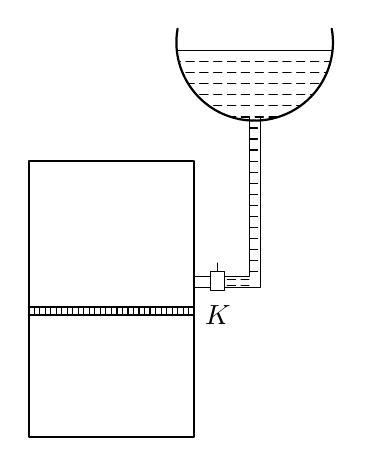
\begin{tikzpicture}[line cap=round, line join=round, >={Stealth}, scale = 0.7]
            % --- Vẽ bình chứa hình chữ nhật chính ---
            \draw[thick] (0,0) rectangle (3,5);
            
            % --- Vẽ Piston ---
            \def\pistonY{2.2} 
            \draw[thick] (0, \pistonY) -- (3, \pistonY);
            \draw[thick] (0, \pistonY + 0.15) -- (3, \pistonY + 0.15);
            \foreach \x in {0.1, 0.2, ..., 2.9} {
                \draw (\x, \pistonY) -- (\x, \pistonY + 0.15);
            }
            
            % --- Vẽ đường ống dẫn ---
            \draw (3, 2.7) -- (4.2, 2.7) -- (4.2, 5.8); 
            \draw (3, 2.9) -- (4.0, 2.9) -- (4.0, 5.8);
            
            % --- Vẽ van K ---
            \draw[fill=white] (3.3, 2.65) rectangle (3.55, 3.0);
            \draw (3.425, 3.0) -- (3.425, 3.15); 
            \node[below=2pt] at (3.425, 2.65) {${K}$};
            
            % --- Vẽ phễu/bình chứa phía trên với kỹ thuật CLIPPING ---
            \begin{scope}[shift={(4.1, 6.8)}]
                % 1. Tạo vùng cắt (Clip) theo hình dạng bên trong phễu
                \begin{scope}
                    % Đường cắt bao gồm cung tròn và đường thẳng nối đỉnh phễu
                    \clip (-1.4, 0.6) arc (170:370:1.42) -- cycle;
                    
                    % 2. Vẽ chất lỏng (Chỉ những phần nằm trong vùng clip mới hiển thị)
                    % Vẽ dư ra ngoài thoải mái, TikZ sẽ tự cắt đi
                    \foreach \y in {0.2, 0, ..., -1.4} {
                        \draw[dash pattern=on 3pt off 2pt] (-1.5, \y) -- (1.5, \y);
                    }
                \end{scope}
                
                % 3. Vẽ thành phễu (Vẽ sau để đường viền rõ nét)
                \draw[thick] (-1.4, 0.6) arc (170:370:1.42);
                
                % Mặt thoáng chất lỏng
                \draw (-1.4, 0.2) -- (1.4, 0.2);
            \end{scope}
            
            % --- Chất lỏng trong ống dẫn (Cũng dùng clip cho gọn) ---
            \begin{scope}
                \clip (4.0, 2.9) rectangle (4.2, 5.8);
                \foreach \y in {3.0, 3.2, ..., 5.7} {
                    \draw[dash pattern=on 3pt off 2pt] (4.0, \y) -- (4.2, \y);
                }
            \end{scope}
            
            % Chất lỏng đoạn nằm ngang
            \begin{scope}
                \clip (3.55, 2.7) rectangle (4.0, 2.9);
                \draw[dash pattern=on 3pt off 2pt] (3.6, 2.75) -- (4.0, 2.75);
                \draw[dash pattern=on 3pt off 2pt] (3.6, 2.85) -- (4.0, 2.85);
            \end{scope}

        \end{tikzpicture}
    }
    \choiceTF[1]
    {Thể tích của khí ở phần trên lúc sau là ${\frac{V}{4}}$}
    {\True Áp suất khí ở phần dưới lúc sau là ${\frac{3}{2} p}$}
    {Áp suất khí ở phần trên lúc sau là ${\frac{5}{4} p}$}
    {\True Khối lượng của chất lỏng chảy vào bình là ${\frac{3pS}{10g}}$}
    \loigiai{
        \begin{itemchoice}
        \itemch Thể tích khí phần trên lúc sau: ${V_{tr} = V - V_{\mathrm{dưới}} - V_{\mathrm{chất\, lỏng}} = V - \frac{V}{3} - \frac{V}{4} = \frac{5V}{12}}$.
        \itemch Đối với phần khí dưới (đẳng nhiệt): ${p \cdot \frac{V}{2} = p_2 \cdot \frac{V}{3} \Rightarrow p_2 = \frac{3}{2} p}$.
        \itemch Đối với phần khí trên (đẳng nhiệt): ${p \cdot \frac{V}{2} = p_1 \cdot \frac{5V}{12} \Rightarrow p_1 = \frac{6}{5} p}$.
        \itemch Khi piston cân bằng: ${p_2 = p_1 + \frac{m_{cl}g}{S} \Rightarrow \frac{3}{2}p = \frac{6}{5}p + \frac{m_{cl}g}{S} \Rightarrow \frac{m_{cl}g}{S} = \frac{3}{10}p \Rightarrow m_{cl} = \frac{3pS}{10g}}$.
        \end{itemchoice}
    }
\end{ex}


% Câu 1
\begin{ex}
    Một khung dây dẫn có diện tích ${0{,}8 \, \mathrm{m^2}}$ trong từ trường đều sao cho mặt phẳng khung dây vuông góc với các đường sức từ. Biết độ lớn cảm ứng từ của từ trường này là ${2 \, \mathrm{T}}$. Độ lớn của từ thông đi qua khung dây này là bao nhiêu ${ \mathrm{Wb} }$?
    \shortans{1,6}
    \loigiai{
        ${\phi = BS = 2 \cdot 0{,}8 = 1{,}6 \, \mathrm{Wb}}$
    }
\end{ex}


% Câu 2
\begin{ex}
    Một bình chứa khí heli có thể tích không đổi, nhiệt độ ban đầu ${27^\circ\mathrm{C}}$. Sau một thời gian có một lượng khí thoát ra ngoài, nhiệt độ khí trong bình giảm còn ${15^\circ\mathrm{C}}$ và áp suất giảm đi ${6\%}$. Tính phần trăm khối lượng khí thoát ra (làm tròn kết quả đến chữ số hàng phần mười)?
    \shortans{2,1}
    \loigiai{
        ${\dfrac{pV}{T} = nR = \dfrac{m}{M}R \Rightarrow \dfrac{m_2}{m_1} = \dfrac{p_2}{p_1} \cdot \dfrac{T_1}{T_2} = (1 - 0{,}06) \cdot \dfrac{27 + 273}{15 + 273} \approx 0{,}979 = 97{,}9\% = 100\% - 2{,}1\%}$
    }
\end{ex}


% Câu 3
\begin{ex}
    Hạt nhân ${^7_3\mathrm{Li}}$ có năng lượng liên kết riêng là ${5{,}63 \, \mathrm{MeV/nucleon}}$. Biết khối lượng của proton và neutron lần lượt là ${1{,}0073 \, \mathrm{amu}}$ và ${1{,}0087 \, \mathrm{amu}}$. Khối lượng của hạt nhân ${^7_3\mathrm{Li}}$ là bao nhiêu ${ \mathrm{amu} }$ (làm tròn kết quả đến chữ số hàng phần trăm)?
    \shortans{7,01}
    \loigiai{
        ${W_{lk} = A W_{lkr} = 7 \cdot 5{,}63 = 39{,}41 \, \mathrm{MeV}}$ \\
        ${W_{lk} = \Delta m c^2 \Rightarrow 39{,}41 = \Delta m \cdot 931{,}5 \Rightarrow \Delta m \approx 0{,}0423 \, \mathrm{u}}$ \\
        ${\Delta m = Z m_p + (A - Z) m_n - m \Rightarrow 0{,}0423 = 3 \cdot 1{,}0073 + (7 - 3) \cdot 1{,}0087 - m \Rightarrow m = 7{,}0144 \, \mathrm{u}}$
    }
\end{ex}


% Câu 4
\begin{ex}
    Một buồng khí không trao đổi nhiệt với môi trường ngoài, được chia thành hai phần I và II với tỉ số thể tích ${V_{\mathrm{I}} : V_{\mathrm{II}} = 1 : 3}$ bằng một vách mỏng. Hai phần cùng chứa một loại khí lí tưởng, áp suất khí ở phần I và II lần lượt là ${3 \, \mathrm{atm}}$ và ${1 \, \mathrm{atm}}$. Bây giờ, bỏ vách mỏng ra thì áp suất của khí trong buồng sau khi đạt trạng thái cân bằng là bao nhiêu ${ \mathrm{atm} }$?
    \shortans{1,5}
    \loigiai{
        ${pV = p_1 V_1 + p_2 V_2 \Rightarrow p \cdot (1 + 3) = 3 \cdot 1 + 1 \cdot 3 \Rightarrow p = 1{,}5 \, \mathrm{atm}}$
    }
\end{ex}


% Câu 5
\begin{ex}
\immini[thm]{
        Như hình vẽ, một ống thủy tinh dẫn nhiệt có hai đầu bịt kín được đặt thẳng đứng. Cột thủy ngân chia khí lí tưởng bên trong thành hai phần, phần trên và phần dưới. Ban đầu, chiều dài của khí phần trên và phần dưới đều là ${l}$, áp suất của khí phần trên là ${p_0}$, và nhiệt độ nhiệt động của môi trường là ${T_0}$. Bây giờ, do nhiệt độ môi trường thay đổi một lượng ${xT_0}$ nên cột thủy ngân hạ xuống một đoạn ${\frac{l}{5}}$. Biết rằng khối lượng của cột thủy ngân là ${\frac{p_0 S}{g}}$, với ${S}$ là tiết diện của ống thủy tinh, ${g}$ là gia tốc trọng trường. Giá trị của ${x}$ là bao nhiêu?
    }{
        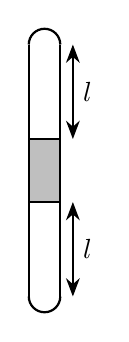
\begin{tikzpicture}[>={Stealth}, thick, scale=0.8]
            \draw (0,0) -- (0,4);
            \draw (0.5,0) -- (0.5,4);
            \draw (0,0) arc (180:360:0.25);
            \draw (0,4) arc (180:0:0.25);
            \draw[fill=gray!50] (0,1.5) rectangle (0.5,2.5);
            \draw[<->] (0.7, 2.5) -- (0.7, 4) node[midway, right] {$l$};
            \draw[<->] (0.7, 0) -- (0.7, 1.5) node[midway, right] {$l$};
        \end{tikzpicture}
    }
    \shortans{0,4}
    \loigiai{
        Áp suất do cột thủy ngân nén xuống là ${\dfrac{mg}{S} = p_0}$ \\
        ${\dfrac{pV}{T} = \text{const} \Rightarrow \left\{\begin{aligned} \dfrac{p_0 Sl}{T_0} &= \dfrac{p S \left(l + \dfrac{l}{5}\right)}{T} \\ \dfrac{(p_0 + p_0) Sl}{T_0} &= \dfrac{(p + p_0) S \left(l - \dfrac{l}{5}\right)}{T} \end{aligned}\right. \Rightarrow \dfrac{1}{2} = \dfrac{p \left(1 + \dfrac{1}{5}\right)}{(p + p_0) \left(1 - \dfrac{1}{5}\right)} \Rightarrow p_0 = 2p}$ \\
        ${\rightarrow \dfrac{2}{T_0} = \dfrac{1 + \dfrac{1}{5}}{T} \Rightarrow T = 0{,}6 T_0 \Rightarrow \Delta T = 0{,}4 T_0}$
    }
\end{ex}


% Câu 6
\begin{ex}
\immini[thm]{
        Như hình bên, một ống hình chữ U tiết diện đều và một piston nhẹ, nhẵn được lắp ở nhánh bên trái tạo thành hai cột không khí dài ${L = 25 \, \mathrm{cm}}$ được chứa trong cả hai nhánh. Áp suất khí quyển là ${76 \, \mathrm{cmHg}}$. Độ cao chênh lệch giữa hai mặt thuỷ ngân trong hai nhánh là ${h = 6 \, \mathrm{cm}}$. Bây giờ, dùng ngoại lực kéo từ từ piston theo phương thẳng đứng hướng lên trên cho đến khi bề mặt thủy ngân trong hai nhánh ngang bằng nhau. Coi nhiệt độ của không khí trong hai nhánh không đổi. Piston đã chuyển động hướng lên trên một đoạn là bao nhiêu ${ \mathrm{cm} }$?
    }{
        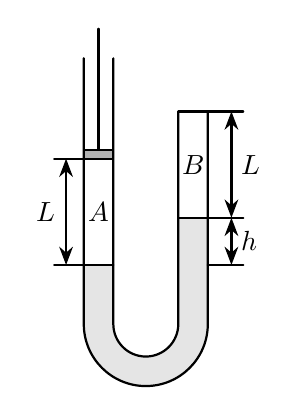
\begin{tikzpicture}[>={Stealth}, thick, scale=0.75, line cap=round, line join=round]
            % --- Khai báo các thông số kích thước ---
            \def\uWidth{1.6}      % Khoảng cách giữa 2 tâm ống
            \def\tubeR{0.25}      % Bán kính lòng ống
            \def\L{1.8}           % Chiều cao cột khí L (đoạn trắng phía trên chất lỏng)
            \def\h{0.8}           % Độ chênh lệch h giữa hai mặt thoáng
            \def\ya{1.0}          % Mực chất lỏng ở nhánh trái (A)
            \def\yb{\ya + \h}     % Mực chất lỏng ở nhánh phải (B) - B cao hơn A theo hình
            \def\ypiston{\ya + \L} % Vị trí piston ở nhánh trái
            \def\ytopB{\yb + \L}   % Đỉnh ống kín bên phải
            \def\tubeH{4.5}       % Chiều cao thành ống trái

            % --- Vẽ phần chất lỏng (vùng màu xám nhạt) ---
            \fill[gray!20] (-\uWidth/2-\tubeR, \ya) -- (-\uWidth/2+\tubeR, \ya) -- (-\uWidth/2+\tubeR, 0)
                arc (180:360:\uWidth/2-\tubeR) -- (\uWidth/2-\tubeR, \yb) -- (\uWidth/2+\tubeR, \yb)
                -- (\uWidth/2+\tubeR, 0) arc (360:180:\uWidth/2+\tubeR) -- cycle;

            % --- Vẽ thành ống ---
            % Thành ống bên trái (hở) và phần đáy cong
            \draw[thick] (-\uWidth/2-\tubeR, \tubeH) -- (-\uWidth/2-\tubeR, 0) 
                arc (180:360:\uWidth/2+\tubeR) -- (\uWidth/2+\tubeR, \ytopB);
            \draw[thick] (-\uWidth/2+\tubeR, \tubeH) -- (-\uWidth/2+\tubeR, 0) 
                arc (180:360:\uWidth/2-\tubeR) -- (\uWidth/2-\tubeR, \ytopB);
            % Đỉnh ống phải (kín)
            \draw[thick] (\uWidth/2-\tubeR, \ytopB) -- (\uWidth/2+\tubeR, \ytopB);

            % --- Vẽ Piston và cần đẩy ---
            \draw[fill=gray!60] (-\uWidth/2-\tubeR, \ypiston) rectangle (-\uWidth/2+\tubeR, \ypiston+0.15);
            \draw[thick] (-\uWidth/2, \ypiston+0.15) -- (-\uWidth/2, \tubeH+0.5);

            % --- Vẽ các đường mặt thoáng chất lỏng ---
            \draw (-\uWidth/2-\tubeR, \ya) -- (-\uWidth/2+\tubeR, \ya);
            \draw (\uWidth/2-\tubeR, \yb) -- (\uWidth/2+\tubeR, \yb);

            % --- Nhãn chữ A và B bên trong các cột khí ---
            \node at (-\uWidth/2, \ya + \L/2) {$A$};
            \node at (\uWidth/2, \yb + \L/2) {$B$};

            % --- Các đường dóng và kích thước ---
            % Nhãn L bên trái
            \def\dx{0.5}
            \draw (-\uWidth/2-\tubeR, \ya) -- (-\uWidth/2-\tubeR-\dx, \ya);
            \draw (-\uWidth/2-\tubeR, \ypiston) -- (-\uWidth/2-\tubeR-\dx, \ypiston);
            \draw[<->] (-\uWidth/2-\tubeR-\dx+0.2, \ya) -- (-\uWidth/2-\tubeR-\dx+0.2, \ypiston) 
                node[midway, left] {$L$};

            % Nhãn L và h bên phải
            \def\dxR{0.6}
            \draw (\uWidth/2+\tubeR, \ytopB) -- (\uWidth/2+\tubeR+\dxR, \ytopB);
            \draw (\uWidth/2+\tubeR, \yb) -- (\uWidth/2+\tubeR+\dxR, \yb);
            \draw (\uWidth/2+\tubeR, \ya) -- (\uWidth/2+\tubeR+\dxR, \ya); % Dóng từ mức A sang phải
            
            % Mũi tên đo đoạn L (phải)
            \draw[<->] (\uWidth/2+\tubeR+\dxR-0.2, \yb) -- (\uWidth/2+\tubeR+\dxR-0.2, \ytopB) 
                node[midway, right] {$L$};
            % Mũi tên đo đoạn h (phải)
            \draw[<->] (\uWidth/2+\tubeR+\dxR-0.2, \ya) -- (\uWidth/2+\tubeR+\dxR-0.2, \yb) 
                node[midway, right] {$h$};

        \end{tikzpicture}
    }
    \shortans{8,4}
    \loigiai{
        \begin{center}
        \begin{tabular}{|l|l|l|l|}
        \hline
        & ${p}$ & ${V}$ & ${T}$ \\ \hline
        Phần A ban đầu & ${p_0 = 76 \, \mathrm{cmHg}}$ & ${SL}$ & ${T_A}$ \\ \hline
        Phần B ban đầu & ${p_0 - h = 76 - 6 = 70 \, \mathrm{cmHg}}$ & ${SL}$ & ${T_B}$ \\ \hline
        Phần A lúc sau & ${p}$ & ${SL_A}$ & ${T_A}$ \\ \hline
        Phần B lúc sau & ${p}$ & ${S \left(L + \dfrac{h}{2}\right) = S \cdot \left(25 + \dfrac{6}{2}\right) = S \cdot 28}$ & ${T_B}$ \\ \hline
        \end{tabular}
        \end{center}
        ${\dfrac{pV}{T} = \text{const} \Rightarrow \left\{\begin{aligned} 76 \cdot SL &= p \cdot SL_A \\ 70 \cdot SL &= p \cdot S \cdot 28 \end{aligned}\right. \Rightarrow \dfrac{76}{70} = \dfrac{L_A}{28} \Rightarrow L_A = 30{,}4 \, \mathrm{cm}}$ \\
        Piston đã chuyển động hướng lên trên một đoạn là ${L_A + \dfrac{h}{2} - L = 30{,}4 + \dfrac{6}{2} - 25 = 8{,}4 \, \mathrm{cm}}$
    }
\end{ex}

% Câu 1
\begin{ex}
    Tia nào sau đây không phải là tia phóng xạ?
    \choice
    {Tia $\gamma$}
    {Tia $\beta^+$}
    {Tia $\alpha$}
    {\True Tia X}
    \loigiai{
        Tia X không phải là tia phóng xạ.
    }
\end{ex}


% Câu 2
\begin{ex}
    Hạt nhân $^{226}_{88}\mathrm{Ra}$ biến đổi thành hạt nhân $^{222}_{86}\mathrm{Rn}$ do phóng xạ
    \choice
    {$\alpha$ và $\beta^-$}
    {$\beta^-$}
    {\True $\alpha$}
    {$\beta^+$}
    \loigiai{
        $^{226}_{88}\mathrm{Ra} \rightarrow ^{4}_{2}\alpha + ^{222}_{86}\mathrm{Rn}$.
    }
\end{ex}


% Câu 3
\begin{ex}
    Trong không khí, tia phóng xạ nào sau đây có tốc độ nhỏ nhất?
    \choice
    {Tia $\gamma$}
    {Tia $\beta^+$}
    {Tia $\beta^-$}
    {\True Tia $\alpha$}
    \loigiai{
        Tia $\alpha$ có tốc độ nhỏ nhất.
    }
\end{ex}


% Câu 4
\begin{ex}
    Cho bốn loại tia: tia X, tia $\gamma$, tia hồng ngoại, tia $\alpha$. Tia không cùng bản chất với ba tia còn lại là
    \choice
    {tia hồng ngoại}
    {tia X}
    {\True tia $\alpha$}
    {tia $\gamma$}
    \loigiai{
        Tia $\alpha$ không phải sóng điện từ.
    }
\end{ex}


% Câu 5
\begin{ex}
    Tia $\alpha$
    \choice
    {\True là dòng các hạt nhân $^{4}_{2}\mathrm{He}$}
    {là dòng các hạt nhân nguyên tử hiđrô}
    {có tốc độ bằng tốc độ ánh sáng trong chân không}
    {không bị lệch khi đi qua điện trường và từ trường}
    \loigiai{
    }
\end{ex}


% Câu 6
\begin{ex}
    Phóng xạ $\beta^-$ là
    \choice
    {phản ứng hạt nhân thu năng lượng}
    {phản ứng hạt nhân không thu và không toả năng lượng}
    {sự giải phóng electron từ lớp electron ngoài cùng của nguyên tử}
    {\True phản ứng hạt nhân toả năng lượng}
    \loigiai{
    }
\end{ex}


% Câu 7
\begin{ex}
    Khi nói về sự phóng xạ, phát biểu nào dưới đây là đúng?
    \choice
    {Sự phóng xạ phụ thuộc vào áp suất tác dụng lên bề mặt của khối chất phóng xạ}
    {Chu kì phóng xạ của một chất phụ thuộc vào khối lượng của chất đó}
    {\True Phóng xạ là phản ứng hạt nhân toả năng lượng}
    {Sự phóng xạ phụ thuộc vào nhiệt độ của chất phóng xạ}
    \loigiai{
    }
\end{ex}


% Câu 8
\begin{ex}
    Hạt nhân $^{14}_{6}\mathrm{C}$ phóng xạ $\beta^-$. Hạt nhân con sinh ra có
    \choice
    {5 proton và 6 neutron}
    {6 proton và 7 neutron}
    {\True 7 proton và 7 neutron}
    {7 proton và 6 neutron}
    \loigiai{
        $^{14}_{6}\mathrm{C} \rightarrow ^{0}_{-1}\mathrm{e} + ^{14}_{7}\mathrm{X} \Rightarrow ^{14}_{7}\mathrm{X}$ có ${7}$ proton và ${7}$ neutron.
    }
\end{ex}


% Câu 9
\begin{ex}
    Đồng vị $^{234}_{92}\mathrm{U}$ sau một chuỗi phóng xạ $\alpha$ và $\beta^-$ biến đổi thành $^{206}_{82}\mathrm{Pb}$, đã phóng ra
    \choice
    {\True 7 hạt $\alpha$ và 4 hạt electron}
    {7 hạt $\alpha$ và 8 hạt electron}
    {14 hạt $\alpha$ và 8 hạt electron}
    {14 hạt $\alpha$ và 4 hạt electron}
    \loigiai{
        $^{234}_{92}\mathrm{U} \rightarrow ^{206}_{82}\mathrm{Pb} + x ^{4}_{2}\alpha + y ^{0}_{-1}\mathrm{e} \Rightarrow \left\{\begin{aligned} 234 &= 206 + 4x \\ 92 &= 82 + 2x - y \end{aligned}\right. \Rightarrow \left\{\begin{aligned} x &= 7 \\ y &= 4 \end{aligned}\right.$
    }
\end{ex}


% Câu 10
\begin{ex}
    Một chất phóng xạ có hằng số phóng xạ là ${1{,}8 \cdot 10^{-9} \, \mathrm{s^{-1}}}$ thì có chu kì bán rã là
    \choice
    {$17{,}6$ năm}
    {$5{,}3$ năm}
    {\True $12{,}2$ năm}
    {$23{,}1$ năm}
    \loigiai{
        $T = \frac{\ln 2}{\lambda} = \frac{\ln 2}{1{,}8 \cdot 10^{-9}} = {385081767 \, \mathrm{s}} \approx {12{,}2}$ năm.
    }
\end{ex}


% Câu 11
\begin{ex}
    Ban đầu có $N_0$ hạt nhân của một mẫu chất phóng xạ nguyên chất có chu kì bán rã $T$. Sau khoảng thời gian $0{,}5 T$, số hạt nhân chưa bị phân rã của mẫu chất phóng xạ này là
    \choice
    {$\frac{N_0}{2}$}
    {\True $\frac{N_0}{\sqrt{2}}$}
    {$\frac{N_0}{4}$}
    {$N_0\sqrt{2}$}
    \loigiai{
        $N = N_0 \cdot 2^{-\frac{t}{T}} = N_0 \cdot 2^{-0{,}5} = \frac{N_0}{\sqrt{2}}$.
    }
\end{ex}


% Câu 12
\begin{ex}
    Trong khoảng thời gian $12 \, \mathrm{h}$, $75\%$ số hạt nhân ban đầu của một đồng vị phóng xạ bị phân rã. Chu kì bán rã của đồng vị đó là
    \choice
    {$5 \, \mathrm{h}$}
    {\True $6 \, \mathrm{h}$}
    {$4 \, \mathrm{h}$}
    {$3 \, \mathrm{h}$}
    \loigiai{
        $\Delta N = N_0 \left( 1 - 2^{-\frac{t}{T}} \right) \Rightarrow 0{,}75 = 1 - 2^{-\frac{12}{T}} \Rightarrow T = 6 \, \mathrm{h}$.
    }
\end{ex}


% Câu 13
\begin{ex}
    $^{14}\mathrm{C}$ là đồng vị phóng xạ có chu kì bán rã $5730$ năm. Các nhà khảo cổ phát hiện hàm lượng nguyên tử $^{14}\mathrm{C}$ trong một cây cổ thụ đã chết chỉ bằng $\frac{1}{4}$ lượng nguyên tử $^{14}\mathrm{C}$ có trong cây đó khi còn sống. Thời gian cây cổ thụ đã chết vào khoảng
    \choice
    {$22920$ năm}
    {\True $11460$ năm}
    {$5730$ năm}
    {$2865$ năm}
    \loigiai{
        $N = N_0 \cdot 2^{-\frac{t}{T}} \Rightarrow \frac{1}{4} = 2^{-\frac{t}{5730}} \Rightarrow T = 11460$ năm.
    }
\end{ex}


% Câu 14
\begin{ex}
    Ban đầu một mẫu chất phóng xạ nguyên chất có khối lượng $m_0$, chu kì bán rã của chất này là $3{,}8$ ngày. Sau $15{,}2$ ngày khối lượng của chất phóng xạ đó còn lại là $2{,}24 \, \mathrm{g}$. Giá trị của $m_0$ là
    \choice
    {\True $35{,}84 \, \mathrm{g}$}
    {$5{,}60 \, \mathrm{g}$}
    {$17{,}92 \, \mathrm{g}$}
    {$8{,}96 \, \mathrm{g}$}
    \loigiai{
        $m = m_0 \cdot 2^{-\frac{t}{T}} \Rightarrow 2{,}24 = m_0 \cdot 2^{-\frac{15{,}2}{3{,}8}} \Rightarrow m_0 = 35{,}84 \, \mathrm{g}$.
    }
\end{ex}


% Câu 15
\begin{ex}
    Giả thiết một chất phóng xạ có hằng số phóng xạ là $\lambda = 2 \cdot 10^{-8} \, \mathrm{s^{-1}}$. Thời gian để số hạt nhân chất phóng xạ đó giảm đi $e$ lần (với $\ln e = 1$) là
    \choice
    {$3{,}5 \cdot 10^7 \, \mathrm{s}$}
    {$2 \cdot 10^{-8} \, \mathrm{s}$}
    {$2{,}8 \cdot 10^{-8} \, \mathrm{s}$}
    {\True $5 \cdot 10^7 \, \mathrm{s}$}
    \loigiai{
        $t = \frac{1}{\lambda} = \frac{1}{2 \cdot 10^{-8}} = 5 \cdot 10^7 \, \mathrm{s}$.
    }
\end{ex}


% Câu 16
\begin{ex}
    Ban đầu, một mẫu quặng chứa urani có khối lượng tổng cộng là $M$, trong đó khối lượng của urani là $m$. Urani trải qua một loạt phân rã với chu kì bán rã $T$ cho sản phẩm cuối cùng là chì. Biết các hạt phóng xạ bay ra khỏi mẫu quặng. Sau khoảng thời gian $T$ thì
    \choice
    {khối lượng chì trong quặng là $\frac{1}{2}m$}
    {\True khối lượng urani trong quặng là $\frac{1}{2}m$}
    {khối lượng quặng là $M - \frac{1}{2}m$}
    {khối lượng quặng là $\frac{1}{2}(M - m)$}
    \loigiai{
        $m = m_0 \cdot 2^{-\frac{t}{T}} = m_0 \cdot 2^{-1} = \frac{1}{2}m_0$.
    }
\end{ex}


% Câu 17
\begin{ex}
    Một chất phóng xạ ban đầu có $N_0$ hạt nhân. Sau 1 năm, còn lại một phần tư số hạt nhân ban đầu chưa phân rã. Sau 1 năm nữa, số hạt nhân còn lại chưa phân rã của chất phóng xạ đó là
    \choice
    {$\frac{N_0}{8}$}
    {\True $\frac{N_0}{16}$}
    {$\frac{N_0}{32}$}
    {$\frac{N_0}{64}$}
    \loigiai{
        $N_1 = N_0 \cdot 2^{-\frac{t_1}{T}} \Rightarrow \frac{1}{4} = 2^{-\frac{1}{T}} \Rightarrow T = 0{,}5$ năm. $N_2 = N_0 \cdot 2^{-\frac{t_2}{T}} = N_0 \cdot 2^{-\frac{2}{0{,}5}} = \frac{N_0}{16}$.
    }
\end{ex}


% Câu 18
\begin{ex}
    Một chất phóng xạ X ban đầu có $N_0$ hạt nhân. Sau 8 giờ, còn lại $\frac{1}{16} N_0$ số hạt nhân X chưa phân rã. Sau 4 giờ kể từ ban đầu, số hạt nhân X đã phân rã trong mẫu phóng xạ đó là
    \choice
    {$\frac{N_0}{4}$}
    {$\frac{N_0}{8}$}
    {\True $\frac{3N_0}{4}$}
    {$\frac{7N_0}{8}$}
    \loigiai{
        $N = N_0 \cdot 2^{-\frac{t_1}{T}} \Rightarrow \frac{1}{16} = 2^{-\frac{8}{T}} \Rightarrow T = 2 \, \mathrm{h}$. $\Delta N = N_0 \left( 1 - 2^{-\frac{t_2}{T}} \right) = N_0 \left( 1 - 2^{-\frac{4}{2}} \right) = \frac{3N_0}{4}$.
    }
\end{ex}


% Câu 1
\begin{ex}
    Trong một mẫu đá được các nhà du hành mang về Trái Đất từ Mặt Trăng, các nhà khoa học phát hiện có $75\%$ potassium $^{40}\mathrm{K}$ ban đầu đã biến thành argon $^{40}\mathrm{Ar}$. Biết rằng, khi được hình thành, mẫu đá không chứa argon; toàn bộ argon được tạo ra có nguồn gốc từ potassium và không hề bị thất thoát vào môi trường. Cho chu kì bán rã của $^{40}_{19}\mathrm{K}$ là $1{,}25 \cdot 10^9$ năm.
    \choiceTF
    {\True $^{40}_{19}\mathrm{K}$ là chất phóng xạ $\beta^+$}
    {Phương trình phóng xạ của $^{40}_{19}\mathrm{K}$ là: $^{40}_{19}\mathrm{K} \longrightarrow ^{40}_{18}\mathrm{Ar} + \beta^-$}
    {\True Hạt nhân argon $^{40}_{18}\mathrm{Ar}$ có 22 hạt neutron}
    {\True Tuổi của mẫu đá đó là $2{,}5$ tỉ năm}
    \loigiai{
        \begin{itemchoice}
        \itemch $^{40}_{19}\mathrm{K} \rightarrow ^{40}_{18}\mathrm{Ar} + ^{0}_{1}\mathrm{e} \Rightarrow$ phóng xạ $\beta^+$.
        \itemch 
        \itemch Hạt nhân argon $^{40}_{18}\mathrm{Ar}$ có $N = A - Z = 40 - 18 = 22$ hạt neutron.
        \itemch $\Delta N = N_0 \left( 1 - 2^{-\frac{t}{T}} \right) \Rightarrow 0{,}75 = 1 - 2^{-\frac{t}{1{,}25 \cdot 10^9}} \Rightarrow t = 2{,}5 \cdot 10^9$ năm.
        \end{itemchoice}
    }
\end{ex}


% Câu 2
\begin{ex}
        Hiện nay, đồng vị phóng xạ $^{18}_{9}\mathrm{F}$ được sử dụng rộng rãi trong việc chẩn đoán các bệnh ung thư nhờ vào công nghệ chụp cắt lớp bằng phát xạ positron (Positron Emission Tomography - PET). Trước khi chụp ảnh PET, bệnh nhân được tiêm liều lượng $^{18}_{9}\mathrm{F}$ thích hợp, tùy theo cân nặng của mỗi người. Biết đồng vị $^{18}_{9}\mathrm{F}$ là chất phóng xạ $\beta^+$ với chu kì bán rã là 110 phút.
    \choiceTF
    {\True Giả sử bệnh nhân được tiêm một liều lượng $^{18}_{9}\mathrm{F}$ xác định. Sau 220 phút kể từ thời điểm tiêm thì liều lượng $^{18}_{9}\mathrm{F}$ giảm còn $25\%$ so với lúc đầu}
    {Mỗi hạt nhân đồng vị $^{18}_{9}\mathrm{F}$ có 9 nucleon}
    {\True Tia phóng xạ $\beta^+$ có bản chất là hạt positron ($^0_1\mathrm{e}$)}
    {\True Phản ứng phân rã của đồng vị $^{18}_{9}\mathrm{F}$ là phản ứng hạt nhân tỏa năng lượng}
    \loigiai{
        \begin{itemchoice}
        \itemch $\frac{N}{N_0} = 2^{-\frac{t}{T}} = 2^{-\frac{220}{110}} = 0{,}25 = 25\%$.
        \itemch $A = 18$.
        \itemch 
        \itemch Phóng xạ là phản ứng hạt nhân tỏa năng lượng.
        \end{itemchoice}
    }
\end{ex}


% Câu 3
\begin{ex}
    Hạt nhân $^{238}_{92}\mathrm{U}$ sau một chuỗi các quá trình phóng xạ $\alpha$ và $\beta^-$ liên tiếp biến đổi thành hạt nhân $^{206}_{82}\mathrm{Pb}$ bền theo phương trình chuỗi phản ứng: $^{238}_{92}\mathrm{U} \rightarrow ^{206}_{82}\mathrm{Pb} + x ^{4}_{2}\mathrm{He} + y ^{0}_{-1}\mathrm{e}$. Trong đó, $x$ và $y$ lần lượt là số lần phóng xạ $\alpha$ và $\beta^-$ trong chuỗi phóng xạ. Trong một mẫu quặng uranium, người ta thấy có lẫn chì $^{206}_{82}\mathrm{Pb}$ cùng với $^{238}_{92}\mathrm{U}$. Biết rằng toàn bộ chì được tạo ra có nguồn gốc từ uranium và không hề bị thất thoát vào môi trường. Cho chu kì bán rã của $^{238}_{92}\mathrm{U}$ là $4{,}47$ tỉ năm.
    \choiceTF
    {\True $x = 8$}
    {\True $y = 6$}
    {\True Nếu tỉ lệ nguyên tử tìm thấy là cứ 1 nguyên tử $^{206}_{82}\mathrm{Pb}$ có 5 nguyên tử $^{238}_{92}\mathrm{U}$ thì tuổi mẫu quặng là $1{,}18$ tỉ năm}
    {\True Nếu tỉ lệ khối lượng tìm thấy là cứ $1 \, \mathrm{g}$ $^{206}_{82}\mathrm{Pb}$ có $5 \, \mathrm{g}$ $^{238}_{92}\mathrm{U}$ thì tuổi mẫu quặng là $1{,}34$ tỉ năm}
    \loigiai{
        \begin{itemchoice}
        \itemch $\left\{\begin{aligned} 238 &= 206 + 4x \\ 92 &= 82 + 2x - y \end{aligned}\right. \Rightarrow \left\{\begin{aligned} x &= 8 \\ y &= 6 \end{aligned}\right.$
        \itemch 
        \itemch $\frac{\Delta N}{N} = \frac{N_0 \left( 1 - 2^{-\frac{t}{T}} \right)}{N_0 \cdot 2^{-\frac{t}{T}}} = 2^{\frac{t}{T}} - 1 \Rightarrow \frac{1}{5} = 2^{\frac{t}{4{,}47}} - 1 \Rightarrow t \approx 1{,}18$ tỉ năm.
        \itemch $\frac{m_{\mathrm{Pb}}}{m_{\mathrm{U}}} = \frac{A_{\mathrm{Pb}}}{A_{\mathrm{U}}} \cdot \frac{N_{\mathrm{Pb}}}{N_{\mathrm{U}}} = \frac{A_{\mathrm{Pb}}}{A_{\mathrm{U}}} \left( 2^{\frac{t}{T}} - 1 \right) \Rightarrow \frac{1}{5} = \frac{206}{238} \left( 2^{\frac{t}{4{,}47}} - 1 \right) \Rightarrow t \approx 1{,}34$ tỉ năm.
        \end{itemchoice}
    }
\end{ex}


% Câu 4
\begin{ex}
    Các nhà khoa học sử dụng phương pháp xác định tuổi bằng đồng vị $^{14}_{6}\mathrm{C}$ để xác định niên đại của một cổ vật làm bằng gỗ. Khi cây còn sống, nhờ sự trao đổi chất với môi trường nên tỉ số giữa số nguyên tử $^{14}_{6}\mathrm{C}$ và số nguyên tử $^{12}_{6}\mathrm{C}$ có trong cây luôn không đổi. Khi cây chết, sự trao đổi chất không còn nữa, tỉ số giữa số nguyên tử $^{14}_{6}\mathrm{C}$ và số nguyên tử $^{12}_{6}\mathrm{C}$ có trong gỗ giảm đi do $^{14}_{6}\mathrm{C}$ là chất phóng xạ $\beta^-$ với chu kì bán rã $5730$ năm. Một mảnh gỗ của cổ vật có số phân rã của $^{14}_{6}\mathrm{C}$ trong 1 giờ là 547. Biết rằng, mảnh gỗ cùng khối lượng của cây cùng loại khi mới chặt có số phân rã của $^{14}_{6}\mathrm{C}$ trong 1 giờ là 855.
    \choiceTF
    {Hằng số phóng xạ của $^{14}_{6}\mathrm{C}$ là $1{,}21 \cdot 10^{-4} \, \mathrm{s^{-1}}$ (làm tròn kết quả đến chữ số hàng phần trăm)}        {\True Phương pháp xác định tuổi bằng đồng vị ${^{14}\mathrm{C}}$ cũng có thể dùng để xác định tuổi của các mẫu xương từ thời cổ đại}
    {\True Tuổi của cổ vật là ${3692}$ năm (làm tròn kết quả đến chữ số hàng đơn vị)}
    {\True Hạt nhân ${^{14}\mathrm{C}}$ phóng ra hạt Electron để biến đổi thành hạt nhân ${^{14}\mathrm{N}}$}
    \loigiai{
        \begin{itemchoice}
            \itemch $\lambda = \frac{\ln 2}{T} = \frac{\ln 2}{5730} \approx 1{,}21 \cdot 10^{-4} \, \mathrm{year^{-1}}$.
            \itemch 
            \itemch ${\left\{\begin{aligned} \Delta N_1 &= N_0 \cdot \left(1 - 2^{-\frac{\Delta t}{T}}\right) \\ \Delta N_2 &= N_0 \cdot 2^{-\frac{t}{T}} \cdot \left(1 - 2^{-\frac{\Delta t}{T}}\right) \end{aligned}\right. \Rightarrow \frac{\Delta N_1}{\Delta N_2} = 2^{\frac{t}{T}} \Rightarrow \frac{855}{547} = 2^{\frac{t}{5730}} \Rightarrow t \approx 3692}$ năm
            \itemch ${^{14}_{6}\mathrm{C} \rightarrow {^0_{-1}\mathrm{e}} + {^{14}_{7}\mathrm{N}}}$
        \end{itemchoice}
    }
\end{ex}

% Câu 1
\begin{ex}
    Chất phóng xạ pôlôni ${^{210}_{84}\mathrm{Po}}$ phát ra tia ${\alpha}$ và biến đổi thành chì ${^{206}_{82}\mathrm{Pb}}$. Biết chu kì bán rã của pôlôni là ${138}$ ngày. Ban đầu có một mẫu pôlôni nguyên chất với ${N_0}$ hạt nhân ${^{210}_{84}\mathrm{Po}}$. Sau bao nhiêu ngày thì có ${0{,}75N_0}$ hạt nhân chì được tạo thành?
    \shortans{276}
    \loigiai{
        ${\Delta N = N_0 \cdot \left(1 - 2^{-\frac{t}{T}}\right) \Rightarrow 0{,}75 = 1 - 2^{-\frac{t}{138}} \Rightarrow t = 276}$ ngày
    }
\end{ex}

% Câu 2
\begin{ex}
    Ban đầu ${(t = 0)}$ có ${N_0}$ hạt nhân của một đồng vị phóng xạ nguyên chất. Sau khoảng thời gian ${10}$ ngày kể từ ${t = 0}$ thì ${\frac{15}{16}}$ số hạt nhân của đồng vị phóng xạ đó đã bị phân rã. Chu kì bán rã của đồng vị phóng xạ này là bao nhiêu ngày?
    \shortans{2,5}
    \loigiai{
        ${\Delta N = N_0 \cdot \left(1 - 2^{-\frac{t}{T}}\right) \Rightarrow \frac{15}{16} = 1 - 2^{-\frac{10}{T}} \Rightarrow T = 2{,}5}$ ngày
    }
\end{ex}

% Câu 3
\begin{ex}
    Chất phóng xạ pôlôni ${^{210}_{84}\mathrm{Po}}$ phát ra tia ${\alpha}$ và biến đổi thành chì ${^{206}_{82}\mathrm{Pb}}$. Biết chu kì bán rã của pôlôni là ${138}$ ngày. Ban đầu ${(t = 0)}$ có một mẫu pôlôni nguyên chất khối lượng ${50 \, \mathrm{mg}}$. Tại thời điểm ${t = 730}$ ngày, khối lượng chì ${^{206}_{82}\mathrm{Pb}}$ được tạo thành là bao nhiêu ${\mathrm{mg}}$ (làm tròn kết quả đến chữ số hàng phần mười)?
    \shortans{47,8}
    \loigiai{
        ${m_{\mathrm{Pb}} = m_0 \cdot \frac{A_{\mathrm{Pb}}}{A_{\mathrm{Po}}} \cdot \left(1 - 2^{-\frac{t}{T}}\right) = 50 \cdot \frac{206}{210} \cdot \left(1 - 2^{-\frac{730}{138}}\right) \approx 47{,}8 \, \mathrm{mg}}$
    }
\end{ex}

% Câu 4
\begin{ex}
    Để đo chu kì bán rã của một chất phóng xạ ${\beta^-}$, người ta dùng máy đếm xung điện. Mỗi khi có một hạt Electron rơi vào máy thì các hệ số đếm của máy tăng thêm một đơn vị. Trong ${6 \, \mathrm{s}}$ đầu tiên máy đếm ghi được ${N}$ xung điện và trong ${12 \, \mathrm{s}}$ tiếp theo máy đếm ghi được thêm ${0{,}7 N}$ xung điện. Chu kì bán rã của chất phóng xạ đó bằng bao nhiêu ${\mathrm{s}}$ (làm tròn kết quả đến chữ số hàng phần trăm)?
    \shortans{5,58}
    \loigiai{
        ${\Delta N = N_0 \cdot \left(1 - 2^{-\frac{t}{T}}\right) \Rightarrow \frac{\Delta N_1}{\Delta N_2} = \frac{1 - 2^{-\frac{t_1}{T}}}{1 - 2^{-\frac{t_2}{T}}} \Rightarrow \frac{N}{N + 0{,}7N} = \frac{1 - 2^{-\frac{6}{T}}}{1 - 2^{\frac{-6-12}{T}}} \Rightarrow T \approx 5{,}58 \, \mathrm{s}}$
    }
\end{ex}

% Câu 5
\begin{ex}
    Chất phóng xạ pôlôni ${^{210}_{84}\mathrm{Po}}$ phát ra tia ${\alpha}$ và biến đổi thành chì ${^{206}_{82}\mathrm{Pb}}$. Gọi chu kì bán rã của pôlôni là ${T}$. Ban đầu ${(t = 0)}$ có một mẫu ${^{210}_{84}\mathrm{Po}}$ nguyên chất. Tại thời điểm ${t = 2{,}5 \, T}$, mẫu phóng xạ còn ${210 \, \mathrm{mg}}$ ${^{210}_{84}\mathrm{Po}}$ chưa phân rã. Lấy khối lượng nguyên tử tính theo đơn vị ${\mathrm{u}}$ bằng số khối của hạt nhân của nguyên tử đó. Trong khoảng thời gian từ ${t = 2{,}5 \, T}$ đến ${t = 3{,}5 \, T}$, lượng ${^{206}_{82}\mathrm{Pb}}$ được tạo thành trong mẫu có khối lượng là bao nhiêu ${\mathrm{mg}}$?
    \shortans{103}
    \loigiai{
        ${m_{\mathrm{Pb}} = m_0 \cdot \frac{A_{\mathrm{Pb}}}{A_{\mathrm{Po}}} \cdot \left(1 - 2^{-\frac{t}{T}}\right) = 210 \cdot \frac{206}{210} \cdot \left(1 - 2^{-1}\right) = 103 \, \mathrm{mg}}$
    }
\end{ex}

% Câu 6
\begin{ex}
    Pôlôni ${^{210}_{84}\mathrm{Po}}$ là chất phóng xạ. Ban đầu có một mẫu ${^{210}_{84}\mathrm{Po}}$ nguyên chất. Khối lượng ${^{210}_{84}\mathrm{Po}}$ trong mẫu ở các thời điểm ${t = t_0, t = t_0 + 3\Delta t}$ và ${t = t_0 + 5\Delta t}$ ${(\Delta t > 0)}$ có giá trị lần lượt là ${m_0, 16 \, \mathrm{g}}$ và ${4 \, \mathrm{g}}$. Giá trị của ${m_0}$ là bao nhiêu ${\mathrm{g}}$?
    \shortans{128}
    \loigiai{
        ${\left\{\begin{aligned} 16 &= m_0 \cdot 2^{-\frac{3\Delta t}{T}} \\ 4 &= m_0 \cdot 2^{-\frac{5\Delta t}{T}} \end{aligned}\right. \Rightarrow \left\{\begin{aligned} 16^5 &= m_0^5 \cdot 2^{-\frac{15\Delta t}{T}} \\ 4^3 &= m_0^3 \cdot 2^{-\frac{15\Delta t}{T}} \end{aligned}\right. \Rightarrow \frac{16^5}{4^3} = m_0^2 \Rightarrow m_0 = 128 \, \mathrm{g}}$
    }
\end{ex}

% Câu 1
\begin{ex}
    Tia $\beta^-$ là dòng các hạt
    \choice
    {hạt nhân ${^4_2\mathrm{He}}$}
    {positron}
    {\True electron}
    {photon}
    \loigiai{
        Tia $\beta^-$ là dòng các electron.
    }
\end{ex}


% Câu 2
\begin{ex}
    Hạt nhân ${^{14}_6\mathrm{C}}$ và hạt nhân ${^{14}_7\mathrm{N}}$ có cùng
    \choice
    {điện tích}
    {\True số nucleon}
    {số proton}
    {số neutron}
    \loigiai{
        Cả hai hạt nhân đều có số khối $A = {14}$, tức là có cùng số nucleon.
    }
\end{ex}


% Câu 3
\begin{ex}
    Phương trình biểu diễn phân rã $\beta^-$ của nguyên tố phóng xạ iốt 131 (${^{131}_{53}\mathrm{I}}$) là
    \choice
    {${^{131}_{53}\mathrm{I}} \to {^{127}_{51}\mathrm{I}} + {^4_2\mathrm{He}}$}
    {\True ${^{131}_{53}\mathrm{I}} \to {^{131}_{54}\mathrm{Xe}} + {^0_{-1}\mathrm{e}^-}$}
    {${^{131}_{53}\mathrm{I}} \to {^{130}_{53}\mathrm{I}} + {^1_0\mathrm{n}}$}
    {${^{131}_{53}\mathrm{I}} \to {^{130}_{52}\mathrm{Te}} + {^1_1\mathrm{H}}$}
    \loigiai{
        Phân rã $\beta^-$ tạo ra electron ${^0_{-1}\mathrm{e}^-}$ và hạt nhân con có số proton tăng thêm 1 đơn vị.
    }
\end{ex}


% Câu 4
\begin{ex}
    Phát biểu nào sau đây đúng?
    \choice
    {Khi một vật tỏa nhiệt thì nhiệt độ của nó phải giảm}
    {Khi nội năng của một vật tăng thì nhiệt độ của nó phải tăng}
    {Nhiệt có thể tự truyền từ vật có nhiệt độ thấp sang vật có nhiệt độ cao}
    {\True Nhiệt có thể tự truyền từ vật có nhiệt độ cao sang vật có nhiệt độ thấp}
    \loigiai{
        Theo nguyên lí II nhiệt động lực học, nhiệt không thể tự truyền từ một vật sang vật nóng hơn.
    }
\end{ex}


% Câu 5
\begin{ex}
    Tương tác từ không xảy ra trong trường hợp nào dưới đây?
    \choice
    {Cho thanh nam châm và một dòng điện không đổi đặt gần nhau}
    {Hai thanh nam châm đặt gần nhau}
    {\True Một thanh nam châm và một thanh đồng đặt gần nhau}
    {Một thanh nam châm và một thanh sắt non đặt gần nhau}
    \loigiai{
        Đồng không có tính từ nên không tương tác với nam châm.
    }
\end{ex}


% Câu 6
\begin{ex}
    Phát biểu nào sau đây đúng?
    \choice
    {Khi khoảng cách giữa hai phân tử nhỏ hơn khoảng cách cân bằng thì tương tác phân tử là hút nhau}
    {Nội năng của một vật là tổng động năng của tất cả các phân tử trong vật đó}
    {\True Một lượng khí lí tưởng nếu áp suất tăng gấp đôi trong quá trình đẳng nhiệt thì thể tích giảm đi một nửa}
    {Nội năng của khí lí tưởng phụ thuộc vào thể tích của khí}
    \loigiai{
        Trong quá trình đẳng nhiệt, áp suất và thể tích tỉ lệ nghịch với nhau.
    }
\end{ex}


% Câu 7
\begin{ex}
    Kết quả thí nghiệm tán xạ hạt alpha của Rutherford
    \choice
    {chứng minh sự tồn tại của proton}
    {chứng minh hạt nhân nguyên tử được cấu tạo từ các proton và neutron}
    {\True cho thấy điện tích dương và hầu hết khối lượng của nguyên tử tập trung trong một hạt nhân rất nhỏ}
    {chứng minh các electron trong nguyên tử chỉ có thể chuyển động theo những quỹ đạo rời rạc nhất định}
    \loigiai{
        Thí nghiệm của Rutherford cho thấy nguyên tử có cấu tạo rỗng, với hạt nhân mang điện tích dương tập trung ở tâm.
    }
\end{ex}


% Câu 8
\begin{ex}
    Quá trình nào sau đây có thể khiến một khối khí lí tưởng trở về áp suất ban đầu?
    \choice
    {\True Làm lạnh đẳng tích rồi nén đẳng nhiệt}
    {Làm lạnh đẳng tích rồi giãn nở đẳng nhiệt}
    {Làm nóng đẳng tích rồi giãn nở đẳng áp}
    {Làm nóng đẳng tích rồi nén đẳng nhiệt}
    \loigiai{
        Làm lạnh đẳng tích thì áp suất $p$ giảm, sau đó nén đẳng nhiệt thì áp suất $p$ tăng trở lại.
    }
\end{ex}


% Câu 9
\begin{ex}
    Trong một xilanh có một lượng khí lí tưởng nhất định được bịt kín bằng một piston. Quá trình thay đổi chậm nào sau đây mà khí có thể không trao đổi nhiệt?
    \choice
    {Thể tích của khí không đổi và nhiệt độ tăng}
    {Thể tích của khí giảm và nhiệt độ giảm}
    {\True Thể tích của khí giảm và nhiệt độ tăng}
    {Thể tích của khí tăng và nhiệt độ không đổi}
    \loigiai{
        Xét trường hợp C: Thể tích của khí giảm $\Rightarrow$ khí nhận công ($A > 0$) và nhiệt độ tăng $\Rightarrow$ nội năng tăng ($\Delta U > 0$). Theo nguyên lí I: $\Delta U = Q + A$, có thể xảy ra trường hợp $Q = 0$.
    }
\end{ex}


% Câu 10
\begin{ex}
    Cường độ dòng điện $i = 2\sqrt{2}\cos(50\pi t) \, (\mathrm{A})$ có chu kì dao động là
    \choice
    {${0{,}4 \, \mathrm{s}}$}
    {\True ${0{,}04 \, \mathrm{s}}$}
    {${0{,}02 \, \mathrm{s}}$}
    {${0{,}2 \, \mathrm{s}}$}
    \loigiai{
        $T = \frac{2\pi}{\omega} = \frac{2\pi}{50\pi} = {0{,}04 \, \mathrm{s}}$.
    }
\end{ex}


% Câu 11
\begin{ex}
    Trộn ${40 \, \mathrm{kg}}$ nước ở ${30^\circ\mathrm{C}}$ và ${10 \, \mathrm{kg}}$ nước ở ${10^\circ\mathrm{C}}$ thì thu được nước ở nhiệt độ là
    \choice
    {${20^\circ\mathrm{C}}$}
    {${24^\circ\mathrm{C}}$}
    {\True ${26^\circ\mathrm{C}}$}
    {${27^\circ\mathrm{C}}$}
    \loigiai{
        $t = \frac{m_1t_1 + m_2t_2}{m_1 + m_2} = \frac{40 \cdot 30 + 10 \cdot 10}{40 + 10} = {26^\circ\mathrm{C}}$.
    }
\end{ex}


% Câu 12
\begin{ex}
    Nén đẳng nhiệt một lượng khí lí tưởng trong xilanh từ thể tích ${9 \, \mathrm{lít}}$ đến thể tích ${6 \, \mathrm{lít}}$, áp suất của khí tăng thêm ${40 \, \mathrm{kPa}}$. Áp suất ban đầu của khí là
    \choice
    {\True ${80 \, \mathrm{kPa}}$}
    {${90 \, \mathrm{kPa}}$}
    {${10^5 \, \mathrm{Pa}}$}
    {${70 \, \mathrm{kPa}}$}
    \loigiai{
        $pV = \mathrm{const} \Rightarrow p \cdot 9 = (p + 40) \cdot 6 \Rightarrow p = {80 \, \mathrm{kPa}}$.
    }
\end{ex}


% Câu 13
\begin{ex}
    Một lượng khí trong một xilanh nhận một nhiệt lượng ${350 \, \mathrm{kJ}}$ và thực hiện công ${130 \, \mathrm{kJ}}$ để đẩy pittông. Độ biến thiên nội năng của lượng khí trong quá trình này là
    \choice
    {\True ${220 \, \mathrm{kJ}}$}
    {${-220 \, \mathrm{kJ}}$}
    {${-480 \, \mathrm{kJ}}$}
    {${480 \, \mathrm{kJ}}$}
    \loigiai{
        $\Delta U = Q + A = 350 - 130 = {220 \, \mathrm{kJ}}$.
    }
\end{ex}


% Câu 14
\begin{ex}
    Năng lượng liên kết của hạt nhân ${^{20}_{10}\mathrm{Ne}}$ là ${160{,}647 \, \mathrm{MeV}}$. Biết khối lượng của hạt proton và hạt neutron lần lượt là ${1{,}0073 \, \mathrm{amu}}$ và ${1{,}0087 \, \mathrm{amu}}$. Khối lượng của hạt nhân ${^{20}_{10}\mathrm{Ne}}$ là
    \choice
    {${19{,}9920 \, \mathrm{amu}}$}
    {\True ${19{,}9875 \, \mathrm{amu}}$}
    {${20{,}0125 \, \mathrm{amu}}$}
    {${20{,}0114 \, \mathrm{amu}}$}
    \loigiai{
        $W_{lk} = \left(10m_p + 10m_n - m\right)c^2 \Rightarrow 160{,}647 = \left(10 \cdot 1{,}0073 + 10 \cdot 1{,}0087 - m\right) \cdot 931{,}5 $\\
        $\Rightarrow m \approx {19{,}9875 \, \mathrm{amu}}$.
    }
\end{ex}


% Câu 15
\begin{ex}
    Thả vật rắn khối lượng $m_1$ nhiệt độ ${150^\circ\mathrm{C}}$ vào một bình chứa nước có khối lượng $m_2$ thì khi cân bằng nhiệt, nhiệt độ của nước tăng từ ${10^\circ\mathrm{C}}$ đến ${50^\circ\mathrm{C}}$. Gọi $c_1$ và $c_2$ lần lượt là nhiệt dung riêng của vật rắn và của nước. Bỏ qua sự hấp thụ nhiệt của bình và môi trường. Tỉ số đúng là
    \choice
    {$\frac{m_1c_1}{m_2c_2} = \frac{7}{2}$}
    {$\frac{m_1c_1}{m_2c_2} = \frac{2}{7}$}
    {$\frac{m_1c_1}{m_2c_2} = \frac{5}{2}$}
    {\True $\frac{m_1c_1}{m_2c_2} = \frac{2}{5}$}
    \loigiai{
        $m_1c_1(150 - 50) = m_2c_2(50 - 10) \Rightarrow 100m_1c_1 = 40m_2c_2 \Rightarrow \frac{m_1c_1}{m_2c_2} = \frac{40}{100} = \frac{2}{5}$.
    }
\end{ex}


% Câu 16
\begin{ex}
    Sau khi đổ nước nóng vào bình và đậy chặt nắp thì khi nước nguội đi sẽ khó mở nắp. Đổ nửa bình nước nóng và vặn chặt nắp thì khí trong bình (coi là khí lí tưởng có khối lượng nhất định) có áp suất $p_0$ ở nhiệt độ ${87^\circ\mathrm{C}}$. Sau một thời gian, nhiệt độ trong bình giảm xuống còn ${27^\circ\mathrm{C}}$. Lúc này áp suất của khí trong bình là
    \choice
    {$\frac{6}{5}p_0$}
    {\True $\frac{5}{6}p_0$}
    {$\frac{29}{9}p_0$}
    {$\frac{9}{29}p_0$}
    \loigiai{
        Đẳng tích $\Rightarrow \frac{p}{T} = \mathrm{const} \Rightarrow \frac{p_0}{87 + 273} = \frac{p}{27 + 273} \Rightarrow \frac{p_0}{360} = \frac{p}{300} \Rightarrow p = \frac{300}{360}p_0 = \frac{5}{6}p_0$.
    }
\end{ex}


% Câu 17
\begin{ex}
    Một quả bóng chuyền có thể tích ${4{,}85 \, \mathrm{lít}}$ chứa không khí có áp suất ${1{,}3 \cdot 10^5 \, \mathrm{Pa}}$ và nhiệt độ ${27^\circ\mathrm{C}}$. Biết khối lượng mol của không khí là ${28{,}8 \, \mathrm{g/mol}}$. Khối lượng không khí có trong quả bóng là
    \choice
    {\True ${7{,}3 \, \mathrm{g}}$}
    {${3{,}7 \, \mathrm{g}}$}
    {${81 \, \mathrm{g}}$}
    {${18 \, \mathrm{g}}$}
    \loigiai{
        $\frac{pV}{T} = nR \Rightarrow \frac{1{,}3 \cdot 10^5 \cdot 4{,}85 \cdot 10^{-3}}{27 + 273} = n \cdot 8{,}31 \Rightarrow n \approx {0{,}2529 \, \mathrm{mol}}$.
        $m = nM = 0{,}2529 \cdot 28{,}8 \approx {7{,}3 \, \mathrm{g}}$.
    }
\end{ex}


% Câu 18
\begin{ex}
    Cho hai phương trình phản ứng hạt nhân: ${X} + {^{14}_7\mathrm{N}} \to {Y} + {^{17}_8\mathrm{O}}$ và ${Y} + {^7_3\mathrm{Li}} \to 2{X}$. Điện tích và số khối của ${X}$ lần lượt là
    \choice
    {1 và 1}
    {1 và 2}
    {2 và 3}
    {\True 2 và 4}
    \loigiai{
        $\left\{\begin{aligned} Z_X + 7 = Z_Y + 8 \\ Z_Y + 3 = 2Z_X \end{aligned}\right. \Rightarrow \left\{\begin{aligned} Z_X = 2 \\ Z_Y = 1 \end{aligned}\right.$\\
        $\left\{\begin{aligned} A_X + 14 = A_Y + 17 \\ A_Y + 7 = 2A_X \end{aligned}\right. \Rightarrow \left\{\begin{aligned} A_X = 4 \\ A_Y = 1 \end{aligned}\right.$
    }
\end{ex}


% Câu 1
\begin{ex}
    Có ba hạt nhân nguyên tử X, Y và Z. Hạt nhân X phát ra một positron thì trở thành hạt nhân Y. Tổng hợp hạt nhân Y với một proton thì tạo ra hạt nhân Z và hạt alpha (${^4_2\mathrm{He}}$).
    \choiceTF
    {Hạt nhân X có nhiều hơn hạt nhân Z một proton}
    {Hạt nhân X có ít hơn hạt nhân Z một neutron}
    {\True Số khối của hạt nhân X lớn hơn số khối của hạt nhân Z là 3}
    {\True Tổng điện tích của hạt nhân X và Z gấp đôi điện tích của hạt nhân Y}
    \loigiai{
        \begin{itemchoice}
        \itemch ${^A_Z\mathrm{X}} \to {^0_{+1}\mathrm{e}} + {^A_{Z-1}\mathrm{Y}}$; ${^A_{Z-1}\mathrm{Y}} + {^1_1\mathrm{p}} \to {^{A-3}_{Z-2}\mathrm{Z}} + {^4_2\mathrm{He}}$. Hạt nhân X có nhiều hơn hạt nhân Z hai proton.
        \itemch Hạt nhân X có $A-Z$ neutron, hạt nhân Z có $(A-3)-(Z-2) = A-Z-1$ neutron $\Rightarrow$ Hạt nhân X có nhiều hơn hạt nhân Z một neutron.
        \itemch Số khối của hạt nhân X là $A$, số khối của hạt nhân Z là $A-3$.
        \itemch Tổng điện tích của hạt nhân X và Z là $Z + (Z-2) = 2Z-2$, điện tích của hạt nhân Y là $Z-1$.
        \end{itemchoice}
    }
\end{ex}


% Câu 2
\begin{ex}
    \immini[thm]{
        Như hình vẽ, hai vòng dây kín $a$ và $b$, được làm từ cùng một loại dây dẫn kim loại. Bán kính của vòng dây $a$ gấp đôi bán kính của vòng dây $b$. Chúng được đặt cố định trong mặt phẳng trang giấy vuông góc với nhau trong từ trường đều biến thiên đều theo thời gian.
    }{
        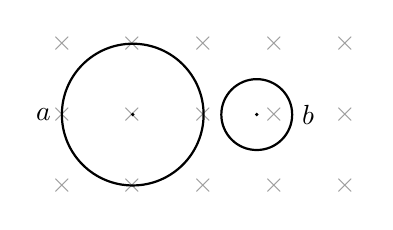
\begin{tikzpicture}[scale=0.45, thick]
            % Draw the grid of crosses representing the magnetic field directed into the page
            \foreach \x in {0,2,4,6,8} {
                \foreach \y in {0,2,4} {
                    \node[gray!80] at (\x, \y) {$\times$};
                }
            }

            % Draw circle 'a'
            \def\ra{2} % Radius of circle a
            \def\xa{2} % x-coordinate of center of circle a
            \def\ya{2}   % y-coordinate of center of circle a
            \draw[thick] (\xa, \ya) circle (\ra);
            \fill (\xa, \ya) circle (1.5pt); % Center dot
            \node[left] at (\xa - \ra, \ya) {$a$}; % Label 'a'

            % Draw circle 'b'
            \def\rb{1} % Radius of circle b
            \def\xb{5.5} % x-coordinate of center of circle b
            \def\yb{2}   % y-coordinate of center of circle b
            \draw[thick] (\xb, \yb) circle (\rb);
            \fill (\xb, \yb) circle (1.5pt); % Center dot
            \node[right] at (\xb + \rb, \yb) {$b$}; % Label 'b'
        \end{tikzpicture}
    }
    \choiceTF
    {Tỉ số giữa từ thông qua vòng dây $a$ và $b$ là $2:1$}
    {\True Tỉ số giữa suất điện động cảm ứng trên vòng dây $a$ và $b$ là $4:1$}
    {\True Tỉ số giữa cường độ dòng điện cảm ứng xuất hiện trong vòng dây $a$ và $b$ là $2:1$}
    {Tỉ số giữa nhiệt lượng tỏa ra từ vòng dây $a$ và $b$ trong cùng khoảng thời gian là $4:1$}
    \loigiai{
        \begin{itemchoice}
        \itemch $S = \pi r^2 \Rightarrow \frac{S_a}{S_b} = \left(\frac{r_a}{r_b}\right)^2 = 2^2 = 4$. $\phi = BS \Rightarrow \frac{\phi_a}{\phi_b} = \frac{S_a}{S_b} = 4$.
        \itemch $e = -\phi' = -B'S \Rightarrow \frac{e_a}{e_b} = \frac{S_a}{S_b} = 4$.
        \itemch $R = \frac{\rho l}{S_{\mathrm{dây}}} = \frac{\rho \cdot 2\pi r}{S_{\mathrm{dây}}} \Rightarrow \frac{R_a}{R_b} = \frac{r_a}{r_b} = 2$. $i = \frac{e}{R} \Rightarrow \frac{i_a}{i_b} = \frac{e_a}{e_b} \cdot \frac{R_b}{R_a} = 4 \cdot \frac{1}{2} = 2$.
        \itemch $Q = i^2Rt \Rightarrow \frac{Q_a}{Q_b} = \left(\frac{i_a}{i_b}\right)^2 \cdot \frac{R_a}{R_b} = 2^2 \cdot 2 = 8$.
        \end{itemchoice}
    }
\end{ex}


% Câu 3
\begin{ex}
    \immini[thm]{
        Một khối khí lí tưởng được cô lập trong một xilanh có piston tiết diện $S$, thành trong của xilanh nhẵn. Ban đầu, dùng sợi dây nhẹ buộc vào tâm piston rồi treo lên trần nhà thì khí có áp suất $\frac{4}{5}p_0$, thể tích $V_0$ và nhiệt độ $T_0$ như hình H1. Bây giờ, cố định xilanh trên một mặt phẳng nghiêng có góc nghiêng là $30^\circ$ như hình H2. Biết áp suất khí quyển là $p_0$, khối lượng của piston và xilanh bằng nhau, gia tốc trọng trường là $g$.
    }{
        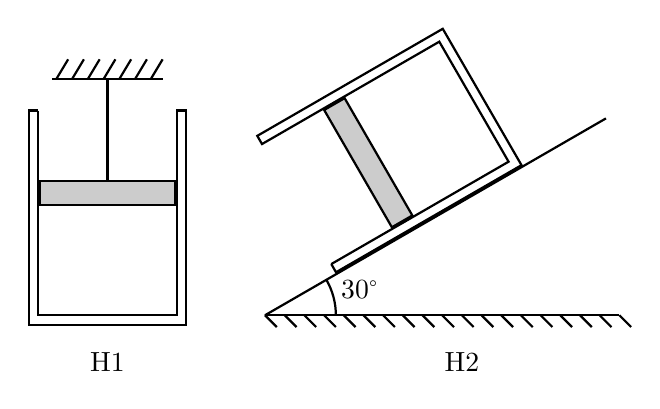
\begin{tikzpicture}[>=latex, thick, scale = 1]

            % --- Diagram H1 ---
            \begin{scope}[shift={(0,0)}]
                % Ceiling with hatching
                \draw[thick] (-0.7, 3.4) -- (0.7, 3.4);
                \foreach \x in {-0.65,-0.45,...,0.65}
                    \draw (\x, 3.4) -- (\x+0.15, 3.65);
                
                % Rod connecting piston to ceiling
                \draw (0, 3.4) -- (0, 2.1);
                
                % Shaded piston
                \draw[fill=gray!40] (-0.86, 1.8) rectangle (0.86, 2.1);
                
                % Cylinder walls (U-shaped container)
                \draw[thick] (-0.88, 3.0) -- (-0.88, 0.4) -- (0.88, 0.4) -- (0.88, 3.0) -- (1.0, 3.0) -- (1.0, 0.28) -- (-1.0, 0.28) -- (-1.0, 3.0) -- (-0.88, 3.0);
                
                % Label H1 centered below
                \node at (0, -0.2) {H1};
            \end{scope}

            % --- Diagram H2 ---
            \begin{scope}[shift={(2,0)}]
                % Horizontal reference line for the angle
                \draw (0, 0.4) -- (4.5, 0.4);
                
                % Inclined plane at 30 degrees
                \draw[thick] (0, 0.4) -- +(30:5) coordinate (plane_top);
                
                % Hatching for the inclined plane
                    \foreach \x in {0,0.25,...,4.5}
                        \draw (\x, 0.4) -- (\x+0.15, 0.25);
                
                % Angle arc and label "30°"
                \draw (0.9, 0.4) arc (0:30:0.9);
                \node at (15:1.25) [shift={(0, 0.4)}] {$30^\circ$};

                % Cylinder and piston system lying on the incline
                \begin{scope}[shift={(4,1.58)}, rotate=120]
                    % Placing the system a bit up the incline
                    \begin{scope}[shift={(2.0, 0)}]
                        % Shaded piston
                        \draw[fill=gray!40] (-0.86, 1.8) rectangle (0.86, 2.1);
                        
                        % Cylinder walls (U-shaped container)
                        \draw[thick] (-0.88, 3.0) -- (-0.88, 0.4) -- (0.88, 0.4) -- (0.88, 3.0) -- (1.0, 3.0) -- (1.0, 0.28) -- (-1.0, 0.28) -- (-1.0, 3.0) -- (-0.88, 3.0);
                    \end{scope}
                \end{scope}
                
                % Label H2 centered roughly below the incline complex
                \node at (2.5, -0.2) {H2};
            \end{scope}

        \end{tikzpicture}
    }
    \choiceTF
    {\True Khối lượng của piston là $\frac{p_0S}{5g}$}
    {Trong hình H2, nếu nhiệt độ của khí vẫn là $T_0$ thì áp suất của khí là $\frac{4}{5}p_0$}
    {Trong hình H2, nếu thể tích khí là $V_0$ thì nhiệt độ của khí là $\frac{8}{9}T_0$}
    {\True Trong hình H2, nếu nhiệt độ khí là $\frac{9}{10}T_0$ thì thể tích của khí là $\frac{4}{5}V_0$}
    \loigiai{
        \begin{itemchoice}
        \itemch H1 xilanh cân bằng: $pS + mg = p_0S \Rightarrow m = \frac{(p_0 - p)S}{g} = \frac{\left(p_0 - \dfrac{4}{5}p_0 \right)S}{g} = \frac{p_0S}{5g}$.
        \itemch H2 piston cân bằng: $pS + mg \sin \alpha = p_0S \Rightarrow p = p_0 - \frac{mg \sin \alpha}{S} = p_0 - \frac{p_0 \sin 30^\circ}{5} = \frac{9p_0}{10}$.
        \itemch Nếu đẳng tích $\Rightarrow \frac{p}{T} = \mathrm{const} \Rightarrow \frac{\dfrac{4}{5}p_0}{T_0} = \frac{\dfrac{9}{10}p_0}{T} \Rightarrow T = \frac{9}{8}T_0$.
        \itemch $\frac{pV}{T} = \mathrm{const} \Rightarrow \frac{\dfrac{4}{5}p_0V_0}{T_0} = \frac{\dfrac{9}{10}p_0V}{\dfrac{9}{10}T_0} \Rightarrow V = \frac{4}{5}V_0$.
        \end{itemchoice}
    }
\end{ex}


% Câu 4
\begin{ex}
    \immini[thm]{
        Một xilanh đủ dài được đặt thẳng đứng như hình vẽ bên. Piston trơn có khối lượng $m = {5{,}5 \, \mathrm{kg}}$ và tiết diện $S = {20 \, \mathrm{cm^2}}$. Piston được nối với đáy xilanh bằng một lò xo nhẹ. Một khối khí lí tưởng được chứa trong xilanh. Ban đầu, lò xo đẩy piston lên với lực có độ lớn $F = {15 \, \mathrm{N}}$, chiều dài lò xo là $l_1 = {12 \, \mathrm{cm}}$, áp suất của khí trong xilanh là $p_1$. Quay chậm xilanh trong mặt phẳng thẳng đứng để miệng xilanh ở phía dưới thì áp suất của khí trong xilanh là $p_2 = {8 \cdot 10^4 \, \mathrm{Pa}}$. Lúc này, chiều dài của lò xo là $l_2$. Biết áp suất khí quyển là $p_0 = {10^5 \, \mathrm{Pa}}$, nhiệt độ của khí trong xilanh không đổi, gia tốc trọng trường là $g = {10 \, \mathrm{m/s^2}}$.
    }{
        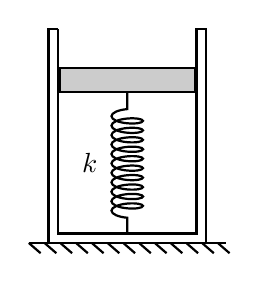
\begin{tikzpicture}[>=latex, thick]
                % Ceiling with hatching
                \draw[thick] (-1.25, 0.28) -- (1.25, 0.28);
                \foreach \x in {-1.25,-1.05,...,1.25}
                    \draw (\x, 0.28) -- (\x+0.15, 0.15);
                
                % Spring
                \draw [decoration={coil, aspect=0.3, segment length=1.2mm, amplitude=2mm, pre length=2mm, post length=2mm}, decorate, thick] (0, 0.4) -- (0, 2.2) node[midway,left=0.25cm]{$k$}; 
                
                % Shaded piston
                \draw[fill=gray!40] (-0.86, 2.2) rectangle (0.86, 2.5);
                
                % Cylinder walls (U-shaped container)
                \draw[thick] (-0.88, 3.0) -- (-0.88, 0.4) -- (0.88, 0.4) -- (0.88, 3.0) -- (1.0, 3.0) -- (1.0, 0.28) -- (-1.0, 0.28) -- (-1.0, 3.0) -- (-0.88, 3.0);
        \end{tikzpicture}
    }
    \choiceTF[1]
    {$p_1 = {1{,}35 \cdot 10^5 \, \mathrm{Pa}}$}
    {Lò xo bị nén trong cả hai trường hợp}
    {\True $l_2 = {18 \, \mathrm{cm}}$}
    {\True Độ cứng lò xo là $k = {500 \, \mathrm{N/m}}$}
    \loigiai{
        \begin{itemchoice}
        \itemch $p_1 = p_0 + \frac{mg - F}{S} = 10^5 + \frac{5{,}5 \cdot 10 - 15}{20 \cdot 10^{-4}} = {1{,}2 \cdot 10^5 \, \mathrm{Pa}}$.
        \itemch Lúc sau miệng xilanh ở phía dưới thì $\left\{\begin{aligned} &p_2S + mg = 8 \cdot 10^4 \cdot 20 \cdot 10^{-4} + 5{,}5 \cdot 10 = {215 \, \mathrm{N}} \\ &p_0S = 10^5 \cdot 20 \cdot 10^{-4} = {200 \, \mathrm{N}} \end{aligned}\right.$ \\${\Rightarrow F' = 215 - 200 = {15 \, \mathrm{N}}}$ cùng chiều $p_0S \Rightarrow F'$ hướng lên $\Rightarrow$ lò xo dãn.
        \itemch $pV = \mathrm{const} \Rightarrow p_1Sl_1 = p_2Sl_2 \Rightarrow 1{,}2 \cdot 10^5 \cdot 12 = 8 \cdot 10^4 \cdot l_2 \Rightarrow l_2 = {18 \, \mathrm{cm}}$.
        \itemch $\left\{\begin{aligned} F = k(l_0 - l_1) \\ F' = k(l_2 - l_0) \end{aligned}\right. \Rightarrow \left\{\begin{aligned} 15 = k(l_0 - 0{,}12) \\ 15 = k(0{,}18 - l_0) \end{aligned}\right. \Rightarrow 30 = k(0{,}18 - 0{,}12) \Rightarrow k = {500 \, \mathrm{N/m}}$.
        \end{itemchoice}
    }
\end{ex}


% Câu 1
\begin{ex}
    Áp suất ban đầu của một lượng khí lí tưởng là ${4 \, \mathrm{atm}}$. Giữ nhiệt độ của khí không đổi, tăng áp suất của khí thêm ${4 \, \mathrm{atm}}$ thì thể tích của khí thay đổi một lượng ${3 \, \mathrm{lít}}$. Thể tích ban đầu của khí là bao nhiêu lít?
    \shortans{6}
    \loigiai{
        $pV = \mathrm{const} \Rightarrow 4V = (4 + 4)(V - 3) \Rightarrow 4V = 8V - 24 \Rightarrow 4V = 24 \Rightarrow V = {6 \, \mathrm{lít}}$.
    }
\end{ex}


% Câu 2
\begin{ex}
    Một cuộn dây hình tròn có 50 vòng. Trong khoảng thời gian ${0{,}01 \, \mathrm{s}}$, từ thông qua mỗi vòng dây giảm đều từ ${60 \, \mathrm{mWb}}$ về ${30 \, \mathrm{mWb}}$. Độ lớn suất điện động cảm ứng xuất hiện trong cuộn dây là bao nhiêu $\mathrm{V}$?
    \shortans{150}
    \loigiai{
        $e = \left| \frac{N\Delta\phi}{\Delta t} \right| = \frac{50 \cdot (60 - 30) \cdot 10^{-3}}{0{,}01} = {150 \, \mathrm{V}}$.
    }
\end{ex}


% Câu 3
\begin{ex}
    Một quả bóng có thể tích không đổi ${8 \, \mathrm{lít}}$, ban đầu chứa không khí ở áp suất ${1 \, \mathrm{atm}}$. Để áp suất khí bên trong quả bóng tăng lên ${4 \, \mathrm{atm}}$ thì cần bơm bao nhiêu lít không khí ở áp suất ${1 \, \mathrm{atm}}$ vào quả bóng (giả sử nhiệt độ không đổi)?
    \shortans{24}
    \loigiai{
        $pV = \mathrm{const} \Rightarrow 1 \cdot (8 + V) = 4 \cdot 8 \Rightarrow 8 + V = 32 \Rightarrow V = {24 \, \mathrm{lít}}$.
    }
\end{ex}


% Câu 4
\begin{ex}
    Một bếp xăng có hiệu suất $30\%$ khi sử dụng để đun nước. Biết năng suất tỏa nhiệt của xăng là ${46 \, \mathrm{kJ/g}}$; nước có nhiệt dung riêng là ${4{,}2 \, \mathrm{J/(g \cdot K)}}$ và nhiệt hóa hơi riêng là ${2256 \, \mathrm{J/g}}$. Để đun sôi ${1 \, \mathrm{kg}}$ nước từ ${20^\circ\mathrm{C}}$ đến ${100^\circ\mathrm{C}}$ và hóa hơi ${0{,}25 \, \mathrm{kg}}$ nước ở nhiệt độ sôi thì phải đốt bao nhiêu gam xăng (làm tròn kết quả đến chữ số hàng phần mười)?
    \shortans{65,2}
    \loigiai{
        $Q = mc\Delta t + m_hL = 10^3 \cdot 4{,}2 \cdot (100 - 20) + 0{,}25 \cdot 10^3 \cdot 2256 = {9 \cdot 10^5 \, \mathrm{J}}$.\\
        $Q_x = \frac{Q}{H} = \frac{9 \cdot 10^5}{0{,}3} = {3 \cdot 10^6 \, \mathrm{J}}$.\\
        $m_x = \frac{Q_x}{q} = \frac{3 \cdot 10^6}{46 \cdot 10^3} \approx {65{,}2 \, \mathrm{g}}$.
    }
\end{ex}


% Câu 5
\begin{ex}
    \immini[thm]{
        Như hình bên, một xilanh hai đầu hở dẫn nhiệt tốt được đặt thẳng đứng. Hai piston $A$ và $B$ được nối với nhau bằng một thanh cứng nhẹ, có diện tích lần lượt là ${20 \, \mathrm{cm^2}}$ và ${40 \, \mathrm{cm^2}}$ và khối lượng lần lượt là ${0{,}5 \, \mathrm{kg}}$ và ${1 \, \mathrm{kg}}$. Piston $A$ được cố định bằng chốt. Khi nhiệt độ môi trường là ${27^\circ\mathrm{C}}$ thì áp suất của khí bên trong xilanh là ${10^5 \, \mathrm{Pa}}$. Biết áp suất khí quyển là ${10^5 \, \mathrm{Pa}}$, gia tốc rơi tự do $g = {10 \, \mathrm{m/s^2}}$ và mọi ma sát đều bỏ qua. Khí bên trong xilanh có thể được coi là khí lí tưởng. Ở nhiệt độ môi trường là bao nhiêu ${^\circ\mathrm{C}}$ thì các piston sẽ đứng yên sau khi chốt được tháo ra (làm tròn kết quả đến chữ số hàng phần mười)?
    }{
        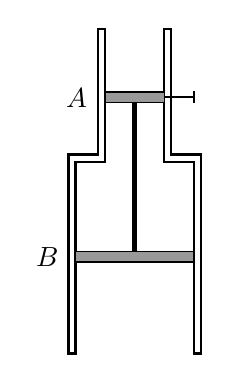
\begin{tikzpicture}[>={Stealth[length=8pt, width=6pt]}, scale = 0.75]
            % Define parameters
            \def\wa{0.5} % Inner half-width of narrow section
            \def\wb{1.0} % Inner half-width of wide section
            \def\wt{0.12} % Wall thickness
            \def\ysep{0.5} % Y-coordinate of the step transition
            \def\yA{1.5} % Y-coordinate of piston A (base)
            \def\yB{-1.2} % Y-coordinate of piston B (base)
            \def\ph{0.18} % Piston height
            % Draw left cylinder walls
            \draw[thick] (-\wa-\wt, 2.75) -- (-\wa-\wt, \ysep+\wt) -- (-\wb-\wt, \ysep+\wt) -- (-\wb-\wt, -2.75) -- (-\wb, -2.75) -- (-\wb, \ysep) -- (-\wa, \ysep) -- (-\wa, 2.75) -- cycle;
            
            % Draw right cylinder walls
            \draw[thick] (\wa+\wt, 2.75) -- (\wa+\wt, \ysep+\wt) -- (\wb+\wt, \ysep+\wt) -- (\wb+\wt, -2.75) -- (\wb, -2.75) -- (\wb, \ysep) -- (\wa, \ysep) -- (\wa, 2.75) -- cycle;
            
            % Draw piston A
            \filldraw[fill=gray!80, draw=black] (-\wa, \yA) rectangle (\wa, \yA+\ph);
            \node[left=0.1cm] at (-\wa, \yA + \ph/2) {$A$};
            
            % Draw piston B
            \filldraw[fill=gray!80, draw=black] (-\wb, \yB) rectangle (\wb, \yB+\ph);
            \node[left=0.1cm] at (-\wb, \yB + \ph/2) {$B$};
            
            % Draw connecting rod
            \draw[ultra thick] (0, \yA) -- (0, \yB+\ph);
            
            % Draw pin/screw at piston A
            \draw[thick] (\wa, \yA + \ph/2) -- (\wa + 0.5, \yA + \ph/2);
            \draw[thick] (\wa + 0.5, \yA + \ph/2 - 0.1) -- (\wa + 0.5, \yA + \ph/2 + 0.1);

        \end{tikzpicture}
    }
    \shortans{4,5}
    \loigiai{
        $p_0S_A + pS_B + (m_A + m_B)g = pS_A + p_0S_B \Rightarrow p = p_0 - \frac{(m_A + m_B)g}{S_B - S_A} = 10^5 - \frac{(0{,}5 + 1) \cdot 10}{(40 - 20) \cdot 10^{-4}} = {92500 \, \mathrm{Pa}}$.\\
        Đẳng tích $\Rightarrow \frac{p}{T} = \mathrm{const} \Rightarrow \frac{10^5}{27 + 273} = \frac{92500}{T} \Rightarrow T = {277{,}5 \, \mathrm{K}} = {4{,}5^\circ\mathrm{C}}$.
    }
\end{ex}


% Câu 6
\begin{ex}
    \immini[thm]{
        Thiết kế một thiết bị thực nghiệm để đo nhiệt độ môi trường xung quanh bằng cân điện tử, như hình vẽ. Xilanh dẫn nhiệt tốt có miệng phía trên được cố định trên bàn. Một khối khí lí tưởng nhất định được bịt kín bởi piston nhẵn có khối lượng $m_1 = {600 \, \mathrm{g}}$ và tiết diện $S = {20 \, \mathrm{cm^2}}$. Tâm của một thanh cứng nhẹ được đặt trên điểm tựa cố định $A$; piston và khối sắt khối lượng $m_2 = {1200 \, \mathrm{g}}$ được treo lần lượt ở đầu bên trái và bên phải của thanh bằng các sợi dây mảnh không dãn, khối sắt được đặt trên cân điện tử. Khi cân điện tử chỉ ${600 \, \mathrm{g}}$ thì nhiệt độ môi trường đo được là $T_1 = {300 \, \mathrm{K}}$. Áp suất khí quyển là ${10^5 \, \mathrm{Pa}}$ và $g = {10 \, \mathrm{m/s^2}}$. Khi cân điện tử chỉ ${400 \, \mathrm{g}}$ thì nhiệt độ môi trường là bao nhiêu $\mathrm{K}$?
    }{
        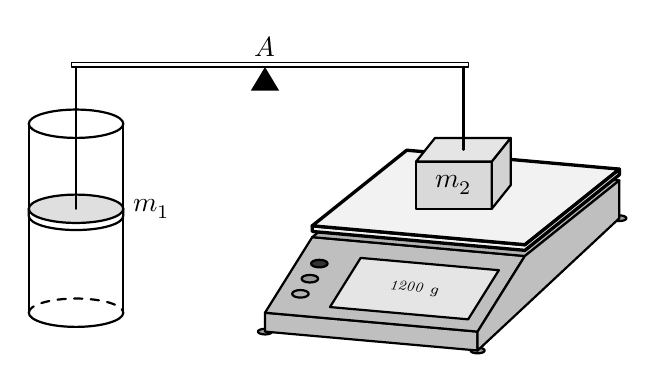
\begin{tikzpicture}[line join=round, line cap=round, scale=0.6, >={Stealth[length=8pt, width=6pt]}, thick]
            % Fulcrum support
            \fill (0,0) -- (-0.3,-0.5) -- (0.3,-0.5) -- cycle;
            \node[above] at (0,0) {$A$};

            % Horizontal Beam
            \draw[fill=white, thin] (-4.1,0) rectangle (4.3,0.1);

            % --- Left Side: Cylinder and Piston ---
            \begin{scope}[shift={(-0.5,-0.7)}]
                % Transparent-like Cylinder
                \draw[thick] (-3.5,-0.5) ellipse (1 and 0.3); % Top opening
                \draw[thick] (-4.5,-0.5) -- (-4.5,-4.5);     % Left wall
                \draw[thick] (-2.5,-0.5) -- (-2.5,-4.5);     % Right wall
                \draw[thick] (-4.5,-4.5) arc (180:360:1 and 0.3); % Bottom front edge
                \draw[thick, dashed] (-4.5,-4.5) arc (180:0:1 and 0.3); % Bottom back edge (hidden)
                
                % Piston inside the cylinder (shaded)
                \filldraw[fill=gray!25, draw=black, thick] (-3.5,-2.3) ellipse (1 and 0.3);
                \draw[thick] (-4.5,-2.3) -- (-4.5,-2.45) arc (180:360:1 and 0.3) -- (-2.5,-2.3);
                \node[right] at (-2.5,-2.3) {$m_1$};
            \end{scope}
            
            % Vertical rod from beam to piston
            \draw (-4,0) -- (-4,-3); 

            % --- Right Side: Weight and Electronic Balance ---
            % Laboratory Electronic Balance
            \begin{scope}[shift={(0,-6)}, xscale = 0.5, yscale = 0.4]
                % Level adjustment feet at the bottom
                \filldraw[fill=gray!80, draw=black] (0, 1) ellipse (0.3 and 0.15);
                \filldraw[gray!80, draw=black] (9, 0) ellipse (0.3 and 0.15);
                \filldraw[gray!80, draw=black] (15, 7) ellipse (0.3 and 0.15);
            
                % Body
                \filldraw[fill=gray!50] (0, 1) -- (9, 0) -- (9, 1) -- (0, 2) -- cycle;
                \filldraw[fill=gray!50] (0, 2) -- (9, 1) -- (11, 5) -- (2, 6) -- cycle;
                \filldraw[fill=gray!60] (2, 6) -- (11, 5) -- (15, 9) -- (6, 10) -- cycle;
                \filldraw[fill=gray!50] (9, 0) -- (9, 1) -- (11, 5) -- (15, 9) -- (15, 7) -- cycle;
            
                % LCD Display area
                \begin{scope}[shift={(2.75,1)}, xscale = 0.65, yscale = 0.65]
                    \filldraw[fill=gray!20] (0, 2) -- (9, 1) -- (11, 5) -- (2, 6) -- cycle;
                \node[rotate=-6.3] at (11/2, 7/2) {\tiny \textit{\textifsym{1200}} ${g}$};
                \end{scope}
            
                % Control Buttons (Tare and Power)
                \filldraw[fill=gray!60, draw=black] (1.5, 3) ellipse (0.35 and 0.2);
                \filldraw[fill=gray!80, draw=black] (1.9, 3.8) ellipse (0.35 and 0.2);
                \filldraw[fill=black!80, draw=black] (2.3, 4.6) ellipse (0.35 and 0.2);
            
                % Balance Pan platform
                \begin{scope}[shift={(2, 6.3)}]
                    \filldraw[fill=gray!10, very thick] (0, 0) -- (9, -1) -- (13, 3) -- (13, 3.3) -- (9, -0.7) -- (0, 0.3) -- cycle;
                    \filldraw[fill=gray!10, very thick] (0, 0.3) -- (9, -0.7) -- (13, 3.3) -- (4, 4.3) -- cycle;
                \end{scope}
            \end{scope}

            % Weight m2 (3D rectangular block)
            \begin{scope}[shift={(4,-2.5)}]
                \filldraw[fill=gray!30, thick] (-0.8,-0.5) rectangle (0.8,0.5); % Front face
                \filldraw[fill=gray!35, thick] (0.8,-0.5) -- (1.2,0) -- (1.2,1) -- (0.8,0.5) -- cycle; % Side face
                \filldraw[fill=gray!20, thick] (-0.8,0.5) -- (-0.4,1) -- (1.2,1) -- (0.8,0.5) -- cycle; % Top face
                \node at (0,0) {$m_2$};
            \end{scope}

            % Vertical rod from beam to weight
            \draw (4.2,0) -- (4.2,-1.75); 
        \end{tikzpicture}
    }
    \shortans{297}
    \loigiai{
        \begin{center}
            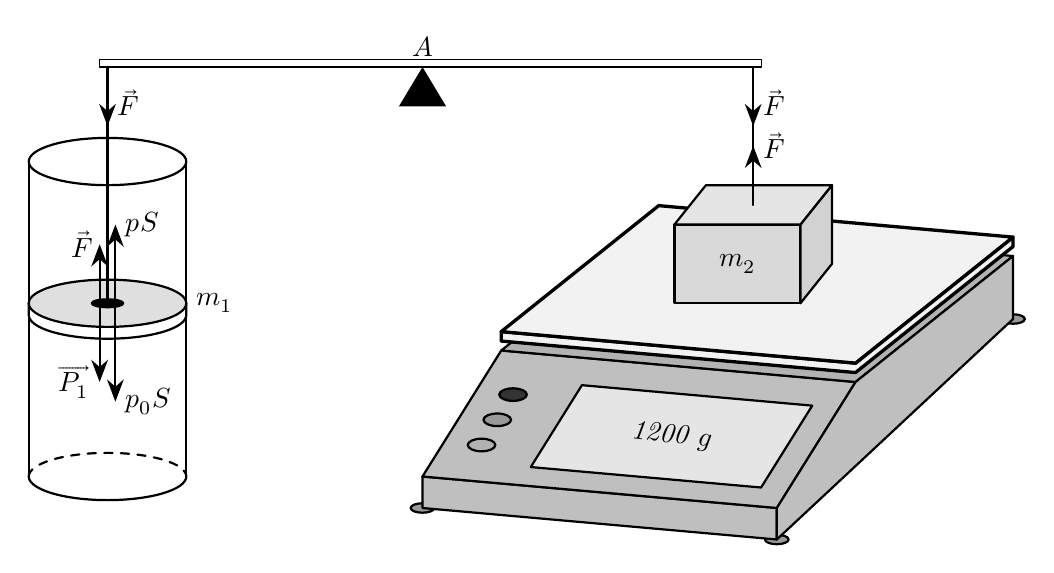
\begin{tikzpicture}[line join=round, line cap=round, scale=1, >={Stealth[length=8pt, width=6pt]}, thick]
                % Fulcrum support
                \fill (0,0) -- (-0.3,-0.5) -- (0.3,-0.5) -- cycle;
                \node[above] at (0,0) {$A$};

                % Horizontal Beam
                \draw[fill=white, thin] (-4.1,0) rectangle (4.3,0.1);

                % --- Left Side: Cylinder and Piston ---
                \begin{scope}[shift={(-0.5,-0.7)}]
                    % Transparent-like Cylinder
                    \draw[thick] (-3.5,-0.5) ellipse (1 and 0.3); % Top opening
                    \draw[thick] (-4.5,-0.5) -- (-4.5,-4.5);     % Left wall
                    \draw[thick] (-2.5,-0.5) -- (-2.5,-4.5);     % Right wall
                    \draw[thick] (-4.5,-4.5) arc (180:360:1 and 0.3); % Bottom front edge
                    \draw[thick, dashed] (-4.5,-4.5) arc (180:0:1 and 0.3); % Bottom back edge (hidden)
                    
                    % Piston inside the cylinder (shaded)
                    \filldraw[fill=gray!25, draw=black, thick] (-3.5,-2.3) ellipse (1 and 0.3);
                    \draw[thick] (-4.5,-2.3) -- (-4.5,-2.45) arc (180:360:1 and 0.3) -- (-2.5,-2.3);
                    \node[right] at (-2.5,-2.3) {$m_1$};
                \end{scope}
                
                % Vertical rod from beam to piston
                \draw (-4,0) -- (-4,-3); 
                \draw[->] (-4,0) -- (-4,-0.75)node[above right] {$\overrightarrow{F}$};
                \draw[->] (-4.1,-3) -- (-4.1,-2.25)node[left] {$\overrightarrow{F}$};
                \draw[->] (-3.9,-3) -- (-3.9,-2)node[right] {$pS$};
                \draw[->] (-4.1,-3) -- (-4.1,-4)node[left] {$\overrightarrow{P_1}$};
                \draw[->] (-3.9,-3) -- (-3.9,-4.25)node[right] {$p_0 S$};
                \filldraw[fill=black, draw=black, thick] (-4,-3) ellipse (0.2 and 0.05);

                % --- Right Side: Weight and Electronic Balance ---
                % Laboratory Electronic Balance
                \begin{scope}[shift={(0,-6)}, xscale = 0.5, yscale = 0.4]
                    % Level adjustment feet at the bottom
                    \filldraw[fill=gray!80, draw=black] (0, 1) ellipse (0.3 and 0.15);
                    \filldraw[gray!80, draw=black] (9, 0) ellipse (0.3 and 0.15);
                    \filldraw[gray!80, draw=black] (15, 7) ellipse (0.3 and 0.15);
                
                    % Body
                    \filldraw[fill=gray!50] (0, 1) -- (9, 0) -- (9, 1) -- (0, 2) -- cycle;
                    \filldraw[fill=gray!50] (0, 2) -- (9, 1) -- (11, 5) -- (2, 6) -- cycle;
                    \filldraw[fill=gray!60] (2, 6) -- (11, 5) -- (15, 9) -- (6, 10) -- cycle;
                    \filldraw[fill=gray!50] (9, 0) -- (9, 1) -- (11, 5) -- (15, 9) -- (15, 7) -- cycle;
                
                    % LCD Display area
                    \begin{scope}[shift={(2.75,1)}, xscale = 0.65, yscale = 0.65]
                        \filldraw[fill=gray!20] (0, 2) -- (9, 1) -- (11, 5) -- (2, 6) -- cycle;
                    \node[rotate=-6.3] at (11/2, 7/2) {\textit{\textifsym{1200}} ${g}$};
                    \end{scope}
                
                    % Control Buttons (Tare and Power)
                    \filldraw[fill=gray!60, draw=black] (1.5, 3) ellipse (0.35 and 0.2);
                    \filldraw[fill=gray!80, draw=black] (1.9, 3.8) ellipse (0.35 and 0.2);
                    \filldraw[fill=black!80, draw=black] (2.3, 4.6) ellipse (0.35 and 0.2);
                
                    % Balance Pan platform
                    \begin{scope}[shift={(2, 6.3)}]
                        \filldraw[fill=gray!10, very thick] (0, 0) -- (9, -1) -- (13, 3) -- (13, 3.3) -- (9, -0.7) -- (0, 0.3) -- cycle;
                        \filldraw[fill=gray!10, very thick] (0, 0.3) -- (9, -0.7) -- (13, 3.3) -- (4, 4.3) -- cycle;
                    \end{scope}
                \end{scope}

                % Weight m2 (3D rectangular block)
                \begin{scope}[shift={(4,-2.5)}]
                    \filldraw[fill=gray!30, thick] (-0.8,-0.5) rectangle (0.8,0.5); % Front face
                    \filldraw[fill=gray!35, thick] (0.8,-0.5) -- (1.2,0) -- (1.2,1) -- (0.8,0.5) -- cycle; % Side face
                    \filldraw[fill=gray!20, thick] (-0.8,0.5) -- (-0.4,1) -- (1.2,1) -- (0.8,0.5) -- cycle; % Top face
                    \node at (0,0) {$m_2$};
                \end{scope}

                % Vertical rod from beam to weight
                \draw (4.2,0) -- (4.2,-1.75); 
                \draw[->] (4.2,0) -- (4.2,-0.75)node[above right] {$\overrightarrow{F}$};
                \draw[->] (4.2,-1.75) -- (4.2, -1) node[right] {$\overrightarrow{F}$};
            \end{tikzpicture}
        \end{center}
        Piston cân bằng $\Rightarrow p_0S + m_1g = pS + F$ (1) và số chỉ của cân là $m_c = \frac{m_2g - F}{g}$ (2).\\
        Từ (1) và (2) $\Rightarrow p = \frac{p_0S + m_1g - (m_2 - m_c)g}{S}$.\\
        $\Rightarrow \left[\begin{aligned} & p_1 = \frac{10^5 \cdot 20 \cdot 10^{-4} + 0{,}6 \cdot 10 - (1{,}2 - 0{,}6) \cdot 10}{20 \cdot 10^{-4}} = {10^5 \, \mathrm{Pa}} \\ & p_2 = \frac{10^5 \cdot 20 \cdot 10^{-4} + 0{,}6 \cdot 10 - (1{,}2 - 0{,}4) \cdot 10}{20 \cdot 10^{-4}} = {9{,}9 \cdot 10^4 \, \mathrm{Pa}} \end{aligned}\right.$\\
        Để thiết bị đo được thì dây không chùng $\Rightarrow$ thể tích khí không đổi $\Rightarrow$ đẳng tích.\\
        $\Rightarrow \frac{p}{T} = \mathrm{const} \Rightarrow \frac{10^5}{300} = \frac{9{,}9 \cdot 10^4}{T_2} \Rightarrow T_2 = {297 \, \mathrm{K}}$.\\
    }
\end{ex}

\begin{ex}
    Vào tháng 03 năm 2011, động đất và sóng thần đã gây hư hại nghiêm trọng nhà máy điện hạt nhân tại Fukushima, Nhật Bản. Sự cố này có thể dẫn đến việc một lượng ...(1)... bị rò rỉ khỏi lò phản ứng. Do đó, hàng ngàn hộ dân đã phải di tản để tránh những tác hại có thể có do chất ...(2)... gây ra. Điền các cụm từ thích hợp vào các chỗ trống.
    \choice
    {(1) hạt nhân; (2) phân hạch}
    {(1) phóng xạ; (2) phân hạch}
    {(1) hạt nhân; (2) phóng xạ}
    {\True (1) phóng xạ; (2) phóng xạ}
    \loigiai{}
\end{ex}


\begin{ex}
    Biển báo nào dưới đây cảnh báo khu vực có chất phóng xạ?
    \begin{center}
        
\begin{tikzpicture}[line join=round, line cap=round]
        \tikzset{warning triangle/.style={fill=yellow, draw=black, line width=4.5pt}}

        % --- BIỂN A: Nguy hiểm điện ---
        \begin{scope}[shift={(0,0)}]
            \draw[warning triangle] (-1,0) -- node[midway, below] {Hình 1} (1,0) -- (0,1.73) -- cycle;
            \fill[black] (-0.1,1.13) -- (-0.25,0.57) -- (0.07,0.71) -- (0,0.5) -- (-0.10,0.56) -- (-0.03,0.22) -- (0.20,0.48) -- (0.10,0.45) -- (0.22,0.87) -- (-0.03,0.77) -- (0.13,1.14) -- (0.18,1.13) -- cycle;
        \end{scope}

        % --- BIỂN B: Phóng xạ ---
        \begin{scope}[shift={(3.5,0)}]
            \draw[warning triangle] (-1,0) -- node[midway, below] {Hình 2} (1,0) -- (0,1.73) -- cycle;
            \begin{scope}[shift={(0,0.6)}, scale = 0.8]
            \fill[black] (0,0) circle (0.12);
            \foreach \a in {90, 210, 330} {
                \fill[black] (\a-30:0.22) arc (\a-30:\a+30:0.22) -- (\a+30:0.65) arc (\a+30:\a-30:0.65) -- cycle;
            }
            \end{scope}
        \end{scope}

        % --- BIỂN C: Nguy hiểm sinh học ---
        \begin{scope}[shift={(7,0)}]
                \draw[warning triangle] (-1,0) -- node[midway, below] {Hình 3} (1,0) -- (0,1.73) -- cycle;
                \begin{scope}[shift={(0,0.6)}, scale=0.4]
                % 2. Vẽ biểu tượng Biohazard ở giữa tam giác    
                % Vẽ 3 vòng tròn lớn (phần thân chính của các móc)
                \foreach \a in {90, 210, 330} {
                \fill[black] (\a:0.7) circle (0.7);
                \fill[yellow] (\a:0.87) circle (0.54);
                }
                % Vẽ vòng tròn ở giữa (hub)
                \draw[black, line width=2pt] (0,0) circle (0.58);
                % Đục một lỗ nhỏ ở chính giữa tâm
                \fill[yellow] (0,0) circle (0.15);
                % Cắt các khe nhỏ ở phần nối giữa các móc và vòng trung tâm
                \foreach \a in {90, 210, 330} {
                \draw[yellow, line width=2pt] (\a:0.15) -- (\a:0.4);
                }
            \end{scope}
        \end{scope}

        % --- BIỂN D: Cảnh báo chung ---
        \begin{scope}[shift={(10.5,0)}]
            \draw[warning triangle] (-1,0) -- node[midway, below] {Hình 4} (1,0) -- (0,1.73) -- cycle;
            \fill[black] (0,1.3) [rounded corners=1.5pt] -- (0.08,1.2) -- (0.04,0.6) -- (-0.04,0.6) -- (-0.08,1.2) -- cycle;
            \fill[black] (0,0.35) circle (0.1);
        \end{scope}
        \end{tikzpicture}
    \end{center}
    \choice
    {Hình 1}
    {\True Hình 2}
    {Hình 3}
    {Hình 4}
    \loigiai{}
\end{ex}


\begin{ex}
    Tháng 3 năm 2015, khi bàn giao tài sản do thay đổi nhân sự phụ trách an toàn bức xạ, một nhà máy thép tại Bà Rịa - Vũng Tàu phát hiện một nguồn phóng xạ $^{60}_{27}\mathrm{Co}$ đã bị thất lạc. Nhà chức trách chỉ đạo phải khẩn cấp tìm nguồn phóng xạ đã bị thất lạc này. Việc khẩn cấp tìm kiếm nguồn phóng xạ $^{60}_{27}\mathrm{Co}$ bị thất lạc là rất quan trọng vì nguồn này
    \choice
    {rất đắt tiền}
    {khó sản xuất nên khó tìm thấy trên thị trường}
    {\True có thể gây nguy hiểm đến sức khoẻ dân cư}
    {cần thiết trong việc khảo sát sát sức bền của thép}
    \loigiai{}
\end{ex}


\begin{ex}
    Nguồn gây ô nhiễm phóng xạ từ đâu?
    \choice
    {Chất thải từ các công trường khai thác chất phóng xạ}
    {Chất thải từ các nhà máy điện nguyên tử, hạt nhân hoặc các chất phóng xạ bị rò rỉ từ các nhà máy này}
    {Hậu quả các vụ thử vũ khí hạt nhân và vũ khí nguyên tử}
    {\True Cả A, B và C}
    \loigiai{}
\end{ex}


\begin{ex}
    Chọn đáp án sai khi nói về những quy tắc an toàn khi làm việc với phóng xạ:
    \choice
    {Giảm thời gian tiếp xúc với nguồn phóng xạ}
    {Tăng khoảng cách từ ta đến nguồn phóng xạ}
    {Đảm bảo che chắn những cơ quan trọng yếu của cơ thể}
    {\True Mang áo phòng hộ và không cần đeo mặt nạ}
    \loigiai{}
\end{ex}


\begin{ex}
    Quy tắc nào là không an toàn khi làm việc với chất phóng xạ là gì?
    \choice
    {\True Tăng thời gian tiếp xúc với nguồn phóng xạ}
    {Tăng khoảng cách từ ta đến nguồn phóng xạ}
    {Đảm bảo che chắn những cơ quan trọng yếu của cơ thể}
    {Kiểm tra sức khỏe định kì}
    \loigiai{}
\end{ex}


\begin{ex}
    Trong hệ đo lường đơn vị quốc tế (SI) đơn vị để đo liều lượng hấp thụ của bức xạ ion hóa là
    \choice
    {\True $\mathrm{J/kg}$, tên là Gray (Gy)}
    {$\mathrm{eV/g}$ hoặc $\mathrm{MeV/kg}$ tên là Rơn-ghen (r)}
    {$\mathrm{Cal/g}$ hoặc $\mathrm{kcal/kg}$, tên là Cu-ri (Ci)}
    {$\mathrm{C/kg}$, tên là Bêch-cor-ren (Bq)}
    \loigiai{}
\end{ex}


\begin{ex}
    Nếu độ phóng xạ của tritium trong một lít nước thải hạt nhân là ${10000} \, \mathrm{Bq}$ thì sau hai chu kì bán rã của tritium, độ phóng xạ của tritium trong một lít nước thải hạt nhân này là
    \choice
    {${7500} \, \mathrm{Bq}$}
    {${5000} \, \mathrm{Bq}$}
    {\True ${2500} \, \mathrm{Bq}$}
    {${1250} \, \mathrm{Bq}$}
    \loigiai{${H = H_0 \cdot 2^{-t/T} = 10000 \cdot 2^{-2} = 2500 \, \mathrm{Bq}}$}
\end{ex}


\begin{ex}
    $^{14}\mathrm{C}$ là chất phóng xạ $\beta^-$ với chu kì bán rã ${5710}$ năm. Một tượng cổ bằng gỗ có độ phóng xạ là $H$. Biết mảnh gỗ cùng khối lượng của cây cùng loại với tượng cổ vừa mới chặt có độ phóng xạ là ${1{,}5}H$. Tuổi của tượng gỗ cổ này là
    \choice
    {\True ${3340}$ năm}
    {${5710}$ năm}
    {${2340}$ năm}
    {${3250}$ năm}
    \loigiai{${H = H_0 \cdot 2^{-t/T} \Rightarrow 1 = 1{,}5 \cdot 2^{-t/5710} \Rightarrow t \approx 3340}$ năm}
\end{ex}


\begin{ex}
    Máy tạo nhịp tim được cung cấp năng lượng từ ``pin tritium''. Pin tritium sử dụng năng lượng hạt nhân được tạo ra bởi sự phân rã của hạt nhân tritium để chuyển hóa thành năng lượng điện. Công suất của máy phụ thuộc vào độ phóng xạ của tritium trong pin. Biết chu kì bán rã của tritium là ${12{,}5}$ năm và khi độ phóng xạ của lượng tritium trong pin thấp hơn ${25\%}$ giá trị ban đầu thì máy sẽ không hoạt động bình thường được. Tuổi thọ của pin năng lượng hạt nhân này vào khoảng
    \choice
    {${20}$ năm}
    {\True ${25}$ năm}
    {${30}$ năm}
    {${35}$ năm}
    \loigiai{${H = H_0 \cdot 2^{-t/T} \Rightarrow 0{,}25 = 2^{-t/12{,}5} \Rightarrow t = 25}$ năm}
\end{ex}


\begin{ex}
    Trong các vụ thử hạt nhân, người ta thấy có đồng vị phóng xạ $^{131}\mathrm{I}$ lan ra trong khí quyển (đồng vị này có thể gây ung thư tuyến giáp). Mưa sẽ làm cỏ nhiễm đồng vị phóng xạ này và cuối cùng nó xuất hiện trong sữa bò. Giả sử sau một vụ thử hạt nhân, người ta đo được độ phóng xạ của $^{131}\mathrm{I}$ trong sữa bò tại một nơi nào đó là ${2900} \, \mathrm{Bq/lít}$. Biết chu kì bán rã của $^{131}\mathrm{I}$ là ${8{,}04}$ ngày. Hỏi sau bao lâu thì sữa bò tại đó mới đạt mức an toàn cho phép là ${185} \, \mathrm{Bq/lít}$?
    \choice
    {${43}$ ngày}
    {${25}$ ngày}
    {${16}$ ngày}
    {\True ${32}$ ngày}
    \loigiai{${H = H_0 \cdot 2^{-t/T} \Rightarrow 185 = 2900 \cdot 2^{-t/8{,}04} \Rightarrow t \approx 32}$ ngày}
\end{ex}


\begin{ex}
    Biết rằng polonium $^{210}_{84}\mathrm{Po}$ có chu kì bán rã ${138}$ ngày. Một mẫu polonium $^{210}_{84}\mathrm{Po}$ có khối lượng $1 \, \mathrm{mg}$ thì có độ phóng xạ là
    \choice
    {\True ${1{,}67 \cdot 10^{11}} \, \mathrm{Bq}$}
    {${1{,}67 \cdot 10^{14}} \, \mathrm{Bq}$}
    {${1{,}44 \cdot 10^{16}} \, \mathrm{Bq}$}
    {${1{,}44 \cdot 10^{13}} \, \mathrm{Bq}$}
    \loigiai{${n = \frac{m}{M} = \frac{10^{-3}}{210} \, \mathrm{mol}}$; \\
    ${N = n N_A = \frac{10^{-3}}{210} \cdot 6{,}02 \cdot 10^{23} \approx 2{,}87 \cdot 10^{18}}$; \\
    ${H = \lambda N = \frac{\ln 2}{T} N = \frac{\ln 2}{138 \cdot 24 \cdot 60 \cdot 60} \cdot 2{,}87 \cdot 10^{18} \approx 1{,}67 \cdot 10^{11} \, \mathrm{Bq}}$}
\end{ex}


\begin{ex}
    Một người tiến hành đo lượng hạt electron phát ra từ một chất phóng xạ $\beta^-$ có chu kì bán rã ${140}$ ngày. Lần đo thứ nhất diễn ra trong khoảng thời gian $1$ phút kể từ $t = 0$, mẫu chất này phát ra $n$ hạt electron. Lần đo thứ hai diễn ra trong khoảng thời gian $1$ phút kể từ thời điểm $t = \tau$, mẫu chất phóng xạ chỉ phát ra $\frac{n}{3}$ hạt electron. Giá trị của $\tau$ là
    \choice
    {\True ${222}$ ngày}
    {${47}$ ngày}
    {${420}$ ngày}
    {${187}$ ngày}
    \loigiai{${\left\{\begin{aligned} & n = N_0 \left( 1 - 2^{-\frac{\Delta t}{T}} \right) \\ & \frac{n}{3} = N_0 \cdot 2^{-\frac{\tau}{T}} \left( 1 - 2^{-\frac{\Delta t}{T}} \right) \end{aligned}\right. \Rightarrow 3 = 2^{\frac{\tau}{T}} \xrightarrow{T=140} \tau \approx 222}$ ngày}
\end{ex}


\begin{ex}
    Ban đầu, hai mẫu chất phóng xạ $A$ và $B$ nguyên chất có khối lượng lần lượt là $m_A$ và $m_B$. Sau đó ${20}$ ngày, lượng chất phóng xạ $A$ và $B$ trong hai mẫu có khối lượng bằng nhau. Biết chu kì bán rã của chất phóng xạ $A$ và $B$ lần lượt là $4$ ngày và $5$ ngày. Tỉ số $\frac{m_A}{m_B}$ bằng
    \choice
    {$\frac{30}{31}$}
    {$\frac{31}{30}$}
    {$\frac{1}{2}$}
    {\True $2$}
    \loigiai{${m = m_A \cdot 2^{-\frac{t}{T_A}} = m_B \cdot 2^{-\frac{t}{T_B}} \Rightarrow \frac{m_A}{m_B} = \frac{2^{-\frac{20}{5}}}{2^{-\frac{20}{4}}} = 2}$}
\end{ex}


\begin{ex}
    Khảo sát đối với hai mẫu chất phóng xạ $A$ và $B$ thì thấy: khi $\frac{15}{16}$ số hạt nhân của mẫu $A$ bị phân rã thì mẫu $B$ có $\frac{63}{64}$ số hạt nhân bị phân rã. Tỉ số giữa chu kì bán rã của mẫu $A$ và chu kì bán rã của mẫu $B$ bằng
    \choice
    {$\frac{20}{21}$}
    {\True $\frac{3}{2}$}
    {$\frac{2}{3}$}
    {$\frac{21}{20}$}
    \loigiai{${\Delta N = N_0 \left( 1 - 2^{-\frac{t}{T}} \right) \Rightarrow \left\{\begin{aligned} & \frac{15}{16} = 1 - 2^{-\frac{t}{T_A}} \\ & \frac{63}{64} = 1 - 2^{-\frac{t}{T_B}} \end{aligned}\right. \Rightarrow t = 4T_A = 6T_B \Rightarrow \frac{T_A}{T_B} = \frac{3}{2}}$}
\end{ex}


\begin{ex}
    Ban đầu, hai mẫu chất phóng xạ $A$ và $B$ có số hạt lần lượt là $N_0$ và $8N_0$. Biết chu kì bán rã của chất phóng xạ $A$ và $B$ lần lượt là $T$ và $\frac{1}{2}T$. Sau đó khoảng thời gian bằng bao nhiêu thì số hạt nhân của chất phóng xạ $A$ và $B$ trong mẫu tương ứng bằng nhau?
    \choice
    {\True $3T$}
    {$2T$}
    {$T$}
    {$4T$}
    \loigiai{${N = N_0 \cdot 2^{-\frac{t}{T_A}} = 8N_0 \cdot 2^{-\frac{t}{T_B}} \Rightarrow 2^{-\frac{t}{T}} = 2^3 \cdot 2^{-\frac{2t}{T}} \Rightarrow -\frac{t}{T} = 3 + \frac{-2t}{T} \Rightarrow t = 3T}$}
\end{ex}


% Câu 17
\begin{ex}
    Một mẫu chất chứa $^{60}\mathrm{Co}$ là chất phóng xạ với chu kì bán rã ${5{,}27}$ năm, được sử dụng trong điều trị ung thư. Gọi $\Delta N_0$ là số hạt nhân $^{60}\mathrm{Co}$ của mẫu phân rã trong ${1}$ phút khi nó mới được sản xuất. Mẫu được coi là hết ``hạn sử dụng'' khi số hạt nhân $^{60}\mathrm{Co}$ của mẫu phân rã trong ${1}$ phút nhỏ hơn ${0{,}7} \Delta N_0$. Nếu mẫu được sản xuất vào tuần đầu tiên của tháng ${8}$ năm ${2020}$ thì ``hạn sử dụng'' của nó đến
    \choice
    {\True tháng ${4}$ năm ${2023}$}
    {tháng ${4}$ năm ${2022}$}
    {tháng ${6}$ năm ${2024}$}
    {tháng ${6}$ năm ${2023}$}
    \loigiai{
        $H = H_0 \cdot 2^{\frac{-t}{T}} \Rightarrow 0{,}7 = 2^{\frac{-t}{5{,}27}} \Rightarrow t \approx 2{,}7118$ năm $\approx 2$ năm $+ 8{,}5$ tháng $\Rightarrow$ tháng ${4}$ năm ${2023}$.
    }
\end{ex}


% Câu 18
\begin{ex}
    Để ước lượng thể tích nước trong một bể nước, một lượng nhỏ dung dịch chứa chất phóng xạ có chu kì bán rã ${3}$ ngày và độ phóng xạ là ${8 \cdot 10^7}$ phân rã/phút được đổ vào bể nước. Sau ${9}$ ngày, lấy mẫu ${1 \, \mathrm{m^3}}$ nước từ bể nước (coi dung dịch chất phóng xạ đã phân bố đều) thì thấy mẫu có độ phóng xạ là ${20}$ phân rã/phút. Thể tích của nước trong bể ước lượng được là
    \choice
    {${3 \cdot 10^5 \, \mathrm{m^3}}$}
    {${4 \cdot 10^5 \, \mathrm{m^3}}$}
    {${2 \cdot 10^5 \, \mathrm{m^3}}$}
    {\True ${5 \cdot 10^5 \, \mathrm{m^3}}$}
    \loigiai{
        $H = H_0 \cdot 2^{\frac{-t}{T}} = 8 \cdot 10^7 \cdot 2^{\frac{-9}{3}} = 10^7$ phân rã/phút $\Rightarrow V = \frac{10^7}{20} = 5 \cdot 10^5 \, \mathrm{m^3}$.
    }
\end{ex}


\begin{ex}
    Các nội dung sau đề cập đến tia phóng xạ.
    \choiceTF[1]
    {Tia phóng xạ $\gamma$ là chùm hạt mang điện dương và có khả năng đâm xuyên rất lớn}
    {\True Nguyên tắc an toàn khi làm việc với nguồn phóng xạ: giữ khoảng cách đủ xa đối với nguồn phóng xạ, cần sử dụng các tấm chắn nguồn phóng xạ đủ tốt và cần giảm thiểu thời gian phơi nhiễm phóng xạ}
    {Các nguồn phóng xạ luôn có hại, nên không để chúng xuất hiện}
    {Tia phóng xạ luôn là chùm hạt mang điện}
    \loigiai{
        \begin{itemchoice}
        \itemch Tia phóng xạ $\gamma$ là sóng điện từ, không mang điện
        \itemch 
        \itemch Phóng xạ có nhiều ứng dụng trong y học, công nghiệp...
        \itemch Tia $\gamma$ không mang điện
        \end{itemchoice}
    }
\end{ex}


\begin{ex}
    Các nội dung sau đề cập đến tính chất của các tia phóng xạ.
    \choiceTF[1]
    {Ta có thể sử dụng một tờ giấy mỏng để ngăn chặn các tia $\gamma$}
    {\True Nếu thâm nhập vào cơ thể chúng ta, chất phóng xạ $\alpha$ sẽ gây nguy hại nhiều hơn so với chất phóng xạ $\gamma$}
    {Một trong các quy tắc an toàn phóng xạ là luôn uống thuốc tân dược để phòng ngừa nhiễm xạ}
    {\True Biển cảnh báo khu vực có chất phóng xạ được đề nghị vào năm 2007 có nhiều thông tin hơn biển cảnh báo năm 1974}
    \loigiai{
        \begin{itemchoice}
        \itemch Tia $\gamma$ có khả năng đâm xuyên mạnh, cần chì hoặc bê tông dày để ngăn chặn
        \itemch Tia $\alpha$ có khả năng ion hóa rất mạnh, gây hại lớn khi ở trong cơ thể
        \itemch 
        \itemch 
        \end{itemchoice}
    }
\end{ex}


% Câu 3
\begin{ex}
    Sau một vụ thử hạt nhân, người ta phát hiện đồng vị phóng xạ $^{131}_{53}\mathrm{I}$ phát tán vào khí quyển. Chất này có thể lắng đọng xuống đất, nhiễm vào cỏ và nguồn nước. Khi một hạt nhân $^{131}_{53}\mathrm{I}$ phân rã, nó phát ra bức xạ $\beta^-$ và biến đổi thành hạt nhân xenon ($\mathrm{Xe}$). Một nông trại nuôi bò có những con bò không may ăn phải cỏ bị nhiễm đồng vị phóng xạ này và rồi sữa bò bị nhiễm phóng xạ. Sau một vụ thử hạt nhân, người ta đo được độ phóng xạ của $^{131}_{53}\mathrm{I}$ trong sữa bò tại trang trại là ${2850 \, \mathrm{Bq/lít}}$. Biết rằng chu kỳ bán rã của $^{131}_{53}\mathrm{I}$ là ${8{,}02}$ ngày và giới hạn an toàn cho mức phóng xạ trong sữa là ${100 \, \mathrm{Bq/lít}}$.
    \choiceTF[1]
    {\True Nếu một người uống sữa chứa $^{131}_{53}\mathrm{I}$ có mức phóng xạ vượt ngưỡng an toàn trong một thời gian dài có thể gây nguy cơ ung thư}
    {Hạt nhân $\mathrm{Xe}$ được sinh ra có ${54}$ proton và ${54}$ neutron}
    {\True Hằng số phóng xạ của $^{131}_{53}\mathrm{I}$ là ${1{,}00 \cdot 10^{-6} \, \mathrm{s^{-1}}}$}
    {Thời gian để mẫu sữa bò tại trang trại đạt mức an toàn phóng xạ cho phép là ${30}$ ngày kể từ thời điểm đo}
    \loigiai{
        \begin{itemchoice}
        \itemch 
        \itemch $^{131}_{53}\mathrm{I} \rightarrow {^0_{-1}}\mathrm{e} + {^{131}_{54}}\mathrm{Xe} \Rightarrow N = A - Z = 131 - 54 = 77$ neutron.
        \itemch $\lambda = \frac{\ln 2}{T} = \frac{\ln 2}{8{,}02 \cdot 24 \cdot 60 \cdot 60} \approx 1{,}00 \cdot 10^{-6} \, \mathrm{s^{-1}}$.
        \itemch $H = H_0 \cdot 2^{\frac{-t}{T}} \Rightarrow 100 = 2850 \cdot 2^{\frac{-t}{8{,}02}} \Rightarrow t \approx 38{,}76$ ngày.
        \end{itemchoice}
    }
\end{ex}


% Câu 4
\begin{ex}
    Một trong số các bụi phóng xạ nguy hiểm từ các vụ nổ hạt nhân là strontium $^{90}_{38}\mathrm{Sr}$ với chu kì bán rã là ${28{,}79}$ năm. Strontium khi bị bò ăn phải sẽ tập trung trong sữa của chúng và sẽ được lưu lại trong xương của những người uống thứ sữa đó. Strontium $^{90}_{38}\mathrm{Sr}$ khi nằm trong xương sẽ phát ra các tia $\beta^-$ có năng lượng lớn phá hủy tủy xương và do đó làm suy yếu sự sản xuất tế bào hồng cầu.
    \choiceTF[1]
    {Hằng số phóng xạ của $^{90}_{38}\mathrm{Sr}$ là ${0{,}024 \, \mathrm{s^{-1}}}$}
    {\True Độ phóng xạ của lượng $^{90}_{38}\mathrm{Sr}$ có khối lượng ${0{,}0145 \, \mathrm{\mu g}}$ là ${74 \, \mathrm{kBq}}$}
    {Khối lượng $^{90}_{38}\mathrm{Sr}$ tích tụ trong xương sẽ giảm ${20\%}$ sau thời gian ${15}$ năm}
    {Hạt nhân Strontium $^{90}_{38}\mathrm{Sr}$ phóng xạ phân rã tạo thành hạt nhân $\mathrm{X}$ bền. Ban đầu ($t = 0$), trong xương có chứa cả hạt nhân $^{90}_{38}\mathrm{Sr}$ và hạt nhân $\mathrm{X}$. Biết hạt nhân $\mathrm{X}$ sinh ra được giữ lại hoàn toàn trong xương. Tại thời điểm $t_1$, tỉ số giữa số hạt nhân $\mathrm{X}$ trong xương và số hạt nhân $^{90}_{38}\mathrm{Sr}$ còn lại là ${1}$. Tại thời điểm $t_2 = 4{,}2 t_1$, tỉ số giữa số hạt nhân $\mathrm{X}$ trong xương và số hạt nhân $^{90}_{38}\mathrm{Sr}$ còn lại là ${3}$. Tỉ số giữa số hạt nhân Strontium $^{90}_{38}\mathrm{Sr}$ và số hạt nhân $\mathrm{X}$ ban đầu là ${0{,}16}$}
    \loigiai{
        \begin{itemchoice}
        \itemch $\lambda = \frac{\ln 2}{T} \approx \frac{\ln 2}{28{,}79 \cdot 365 \cdot 24 \cdot 60 \cdot 60} \approx 7{,}63 \cdot 10^{-10} \, \mathrm{s^{-1}}$.
        \itemch $N_0 = n N_A = \frac{m}{M} N_A = \frac{0{,}0145 \cdot 10^{-6}}{90} \cdot 6{,}02 \cdot 10^{23} \approx 9{,}7 \cdot 10^{13}$. \\
        $H_0 = \lambda N_0 = 7{,}63 \cdot 10^{-10} \cdot 9{,}7 \cdot 10^{13} \approx 74 \cdot 10^3 \, \mathrm{Bq} \approx 74 \, \mathrm{kBq}$.
        \itemch $\Delta m = m_0 \left( 1 - 2^{\frac{-t}{T}} \right) \Rightarrow 0{,}2 = 1 - 2^{\frac{-15}{28{,}79}} \Rightarrow t \approx 9{,}27$ năm.
        \itemch $\frac{N_{0X} + N_0 - N}{N} = \frac{N_{0X} + N_0 - N_0 \cdot 2^{\frac{-t}{T}}}{N_0 \cdot 2^{\frac{-t}{T}}} = \left( \frac{N_{0X}}{N_0} + 1 \right) \cdot 2^{\frac{t}{T}} - 1$. \\
        ${\Rightarrow \left\{\begin{aligned} & \left( \frac{N_{0X}}{N_0} + 1 \right) \cdot 2^{\frac{t_1}{T}} - 1 = 1 \\ & \left( \frac{N_{0X}}{N_0} + 1 \right) \cdot 2^{\frac{4{,}2 t_1}{T}} - 1 = 3 \end{aligned}\right. \Rightarrow \left\{\begin{aligned} & \left( \frac{N_{0X}}{N_0} + 1 \right) \cdot 2^{\frac{t_1}{T}} = 2 \\ & \left( \frac{N_{0X}}{N_0} + 1 \right) \cdot 2^{\frac{4{,}2 t_1}{T}} = 4 \end{aligned}\right. \Rightarrow 2^{\frac{3{,}2 t_1}{T}} = \frac{4}{2} \Rightarrow \frac{t_1}{T} = \frac{1}{3{,}2} \Rightarrow \frac{N_0}{N_{0X}} \approx 1{,}6}$.
        \end{itemchoice}
    }
\end{ex}


% Câu 1
\begin{ex}
    Một chất phóng xạ có chu kì bán rã ${10 \, \mathrm{s}}$, độ phóng xạ ban đầu là ${2 \cdot 10^7 \, \mathrm{Bq}}$. Độ phóng xạ của chất sau đó ${30 \, \mathrm{s}}$ bằng bao nhiêu $\mathrm{MBq}$?
    \shortans{2,5}
    \loigiai{
        $H = H_0 \cdot 2^{\frac{-t}{T}} \Rightarrow H = 2 \cdot 10^7 \cdot 2^{\frac{-30}{10}} = 2{,}5 \cdot 10^6 \, \mathrm{Bq} = 2{,}5 \, \mathrm{MBq}$.
    }
\end{ex}


% Câu 2
\begin{ex}
    Biết rằng độ phóng xạ của ${1 \, \mathrm{g}}$ radium $^{226}\mathrm{Ra}$ là ${3{,}7 \cdot 10^{10} \, \mathrm{Bq}}$. Chu kì bán rã của radium $^{226}\mathrm{Ra}$ là bao nhiêu nghìn năm (làm tròn kết quả đến chữ số hàng phần mười)?
    \shortans{1,6}
    \loigiai{
        $n = \frac{m}{M} = \frac{1}{226} \, \mathrm{mol}$. \\
        $N = n N_A = \frac{1}{226} \cdot 6{,}02 \cdot 10^{23} \approx 2{,}66 \cdot 10^{21}$. \\
        $H = \lambda N = \frac{\ln 2}{T} N \Rightarrow 3{,}7 \cdot 10^{10} = \frac{\ln 2}{T} \cdot 2{,}66 \cdot 10^{21} \Rightarrow T \approx 5 \cdot 10^{10} \, \mathrm{s} \approx 1{,}6 \cdot 10^3$ năm.
    }
\end{ex}


% Câu 3
\begin{ex}
    Silic $^{31}\mathrm{Si}$ là chất phóng xạ, phát ra hạt electron và biến đổi thành hạt nhân $\mathrm{X}$. Một mẫu phóng xạ $^{31}\mathrm{Si}$ ban đầu trong thời gian ${5}$ phút có ${190}$ nguyên tử bị phân rã, nhưng sau đó ${3}$ giờ cũng trong thời gian ${5}$ phút chỉ có ${85}$ nguyên tử bị phân rã. Chu kì bán rã của chất phóng xạ bằng bao nhiêu giờ (làm tròn kết quả đến chữ số hàng phần mười)?
    \shortans{2,6}
    \loigiai{
        $H = H_0 \cdot 2^{\frac{-t}{T}} \Rightarrow 85 = 190 \cdot 2^{\frac{-3}{T}} \Rightarrow T \approx 2{,}6 \, \mathrm{h}$.
    }
\end{ex}


% Câu 4
\begin{ex}
    Để đo chu kì bán rã của một chất phóng xạ $\beta^-$, người ta dùng máy đếm electron. Sau ${2}$ giờ, máy đếm được $N_1$ phân rã/giây. Sau ${6}$ giờ, máy đếm được $N_2$ phân rã/giây. Với $N_1 = 2{,}3 N_2$. Chu kì bán rã của chất phóng xạ bằng bao nhiêu giờ (làm tròn kết quả đến chữ số hàng phần trăm)?
    \shortans{3,33}
    \loigiai{
        $\left\{\begin{aligned} & N_1 = H_0 \cdot 2^{\frac{-t_1}{T}} \\ & N_2 = H_0 \cdot 2^{\frac{-t_2}{T}} \end{aligned}\right. \Rightarrow \frac{N_1}{N_2} = \frac{2^{\frac{-t_1}{T}}}{2^{\frac{-t_2}{T}}} \Rightarrow 2{,}3 = \frac{2^{\frac{-2}{T}}}{2^{\frac{-6}{T}}} \Rightarrow T \approx 3{,}33 \, \mathrm{h}$.\\
    }
\end{ex}


% Câu 5
\begin{ex}
\sochc{2}{Thành phần sữa bò có chứa potassium với nồng độ ${2{,}00 \, \mathrm{g/l}}$. Trong đó, có ${0{,}0117\%}$ là đồng vị phóng xạ potassium $^{40}_{19}\mathrm{K}$ với chu kì bán rã là ${1{,}25 \cdot 10^9}$ năm. Sau tai nạn ở nhà máy điện hạt nhân Chernobyl vào năm ${1986}$, người ta thấy có các đồng vị phóng xạ $^{131}_{53}\mathrm{I}$ trong khí quyển. Biết chu kì bán rã của $^{131}_{53}\mathrm{I}$ là ${8{,}02}$ ngày. Mưa sẽ làm cỏ nhiễm đồng vị phóng xạ này và cuối cùng nó xuất hiện trong sữa bò. Người ta đo được độ phóng xạ của $^{131}_{53}\mathrm{I}$ trong sữa bò ở Ba Lan lúc đó là ${2{,}00 \, \mathrm{kBq/l}}$. Độ phóng xạ này lớn hơn độ phóng xạ của $^{40}_{19}\mathrm{K}$ trong sữa $x$ lần. Xem khối lượng mol tính theo gam bằng số khối của hạt nhân đó. Xem ${1}$ năm có ${365{,}2422}$ ngày.}
    \begin{chc}
        Giá trị $x$ bằng bao nhiêu (làm tròn kết quả đến chữ số hàng phần mười)?
        \shortans{32,3}
        \loigiai{
            Xét ${1}$ lít sữa có $m_s = VD = 1 \cdot 2 = 2 \, \mathrm{g}$. \\
            $m_{\mathrm{K}} = \frac{0{,}0117}{100} \cdot m_s = \frac{0{,}0117}{100} \cdot 2 = 2{,}34 \cdot 10^{-4} \, \mathrm{g}$. \\
            $n = \frac{m_{\mathrm{K}}}{M} = \frac{2{,}34 \cdot 10^{-4}}{40} = 5{,}85 \cdot 10^{-6} \, \mathrm{mol}$. \\
            $N = n N_A = 5{,}85 \cdot 10^{-6} \cdot 6{,}02 \cdot 10^{23} \approx 3{,}522 \cdot 10^{18}$. \\
            $H = \lambda N = \frac{\ln 2}{T_{\mathrm{K}}} \cdot N = \frac{\ln 2}{1{,}25 \cdot 10^9 \cdot 365{,}2422 \cdot 24 \cdot 60 \cdot 60} \cdot 3{,}522 \cdot 10^{18} \approx 61{,}9 \, \mathrm{Bq}$. \\
            $x = \frac{H'}{H} = \frac{2 \cdot 10^3}{61{,}9} \approx 32{,}3$.
        }
    \end{chc}
    \begin{chc}
        Sau bao nhiêu ngày thì độ phóng xạ trong sữa bò do $^{131}_{53}\mathrm{I}$ giảm xuống bằng độ phóng xạ do $^{40}_{19}\mathrm{K}$ (làm tròn kết quả đến chữ số hàng phần mười)?
        \shortans{40,2}
        \loigiai{
            $H = H' \cdot 2^{\frac{-t}{T_{\mathrm{I}}}} \Rightarrow 61{,}9 = 2 \cdot 10^3 \cdot 2^{\frac{-t}{8{,}02}} \Rightarrow t \approx 40{,}2$ ngày.
        }
    \end{chc}
\end{ex}

% Câu 1
\begin{ex}
    Số nucleon có trong hạt nhân ${_{11}^{23}\mathrm{Na}}$ là
    \choice
    {${34}$}
    {${12}$}
    {${11}$}
    {\True ${23}$}
    \loigiai{}
\end{ex}


% Câu 2
\begin{ex}
    Khi nói về các tia phóng xạ, phát biểu nào sau đây là sai?
    \choice
    {Tia ${\beta^+}$ là các dòng positron}
    {\True Tia ${\alpha}$ là các dòng hạt nhân ${_{1}^{2}\mathrm{H}}$}
    {Tia ${\beta^-}$ là dòng các electron}
    {Tia ${\gamma}$ có bản chất là sóng điện từ}
    \loigiai{
        Tia ${\alpha}$ là các dòng hạt nhân ${_{2}^{4}\mathrm{He}}$
    }
\end{ex}


% Câu 3
\begin{ex}
    Gọi ${p, V, T}$ lần lượt là áp suất, thể tích và nhiệt độ tuyệt đối của một khối khí lí tưởng xác định. Công thức nào sau đây mô tả đúng định luật Boyle?
    \choice
    {${\frac{V}{T} = \text{hằng số}}$}
    {\True ${pV = \text{hằng số}}$}
    {${VT = \text{hằng số}}$}
    {${\frac{p}{T} = \text{hằng số}}$}
    \loigiai{
    }
\end{ex}


% Câu 4
\begin{ex}
    Đối với một lượng khí lí tưởng nhất định có thể tích không đổi, nếu nhiệt độ nhiệt động của khí tăng lên gấp đôi thì
    \choice
    {\True Áp suất của khí tăng gấp đôi}
    {Áp suất của khí giảm đi một nửa}
    {Áp suất của khí có thể không thay đổi}
    {Tích của áp suất và thể tích khí không đổi}
    \loigiai{
        Đẳng tích ${\Rightarrow p}$ tỉ lệ thuận với ${T}$
    }
\end{ex}


% Câu 5
\begin{ex}
    Hai kim loại $A$ và $B$ cùng nhiệt độ ban đầu hấp thụ cùng một nhiệt lượng và không chuyển thể. Biết nhiệt dung riêng của $A$ lớn hơn nhiệt dung riêng của $B$. Phát biểu nào sau đây đúng?
    \choice
    {Độ tăng nhiệt độ của $A$ lớn hơn}
    {Độ tăng nhiệt độ của $B$ lớn hơn}
    {Độ tăng nhiệt độ của $A$ và $B$ phải khác nhau}
    {\True Độ tăng nhiệt độ của $A$ và $B$ có thể bằng nhau}
    \loigiai{
        ${Q = mc\Delta t \xrightarrow{c_A > c_B} \Delta t}$ bằng nhau hay không phụ thuộc vào ${m}$
    }
\end{ex}


% Câu 6
\begin{ex}
    Một khối khí lí tưởng nhất định, hấp thụ nhiệt lượng ${500 \, \mathrm{J}}$ và thực hiện công ${100 \, \mathrm{J}}$ thì
    \choice
    {\True nhiệt độ phải tăng}
    {áp suất phải tăng}
    {nội năng không đổi}
    {thể tích phải giảm}
    \loigiai{
        ${\Delta U = Q + A = 500 - 100 = 400 \, \mathrm{J} \Rightarrow}$ nội năng tăng ${\Rightarrow}$ nhiệt độ tăng
    }
\end{ex}


% Câu 7
\begin{ex}
    Cho phân rã: ${_{92}^{A}X \to {}_{Z}^{228}Y + \alpha}$. Giá trị ${Z}$ và ${A}$ lần lượt là
    \choice
    {${94}$ và ${232}$}
    {${94}$ và ${224}$}
    {\True ${90}$ và ${232}$}
    {${90}$ và ${224}$}
    \loigiai{
        ${\left\{\begin{aligned} & A = 228 + 4 \\ & 92 = Z + 2 \end{aligned}\right. \Rightarrow \left\{\begin{aligned} & A = 232 \\ & Z = 90 \end{aligned}\right.}$
    }
\end{ex}


% Câu 8
\begin{ex}
    Nếu ${x}$ biểu thị số electron bên ngoài hạt nhân trong một nguyên tử trung hòa, ${y}$ và ${z}$ lần lượt biểu thị số proton và số neutron trong hạt nhân của nguyên tử; thì đối với nguyên tử ${_{90}^{234}\mathrm{Th}}$ có
    \choice
    {${x = 90, y = 90, z = 234}$}
    {\True ${x = 90, y = 90, z = 144}$}
    {${x = 144, y = 144, z = 90}$}
    {${x = 234, y = 234, z = 324}$}
    \loigiai{
        ${x = y = 90}$ và ${z = A - Z = 234 - 90 = 144}$
    }
\end{ex}


% Câu 9
\begin{ex}
    Một sóng điện từ truyền qua điểm $M$ trong không gian. Cường độ điện trường và cảm ứng từ tại $M$ có giá trị cực đại lần lượt là ${E_0}$ và ${B_0}$. Khi cảm ứng từ tại $M$ là ${\frac{\sqrt{3}}{2} B_0}$ thì cường độ điện trường tại đó là
    \choice
    {\True ${\frac{\sqrt{3}}{2} E_0}$}
    {${\frac{1}{2} E_0}$}
    {${\frac{\sqrt{2}}{2} E_0}$}
    {${\frac{2}{\sqrt{3}} E_0}$}
    \loigiai{
        ${\frac{E}{E_0} = \frac{B}{B_0} = \frac{\sqrt{3}}{2}}$
    }
\end{ex}


% Câu 10
\begin{ex}
    Trộn ${50 \, \mathrm{g}}$ nước nóng ở ${90^\circ\mathrm{C}}$ với ${90 \, \mathrm{g}}$ nước lạnh ở ${20^\circ\mathrm{C}}$ thì thu được nước có nhiệt độ là
    \choice
    {${30^\circ\mathrm{C}}$}
    {\True ${45^\circ\mathrm{C}}$}
    {${55^\circ\mathrm{C}}$}
    {${65^\circ\mathrm{C}}$}
    \loigiai{
        ${t = \frac{m_1 t_1 + m_2 t_2}{m_1 + m_2} = \frac{50 \cdot 90 + 90 \cdot 20}{50 + 90} = 45^\circ\mathrm{C}}$
    }
\end{ex}


% Câu 11
\begin{ex}
    Khi nhiệt độ của khí lí tưởng tăng lên từ ${27^\circ\mathrm{C}}$ đến ${927^\circ\mathrm{C}}$ thì tốc độ căn quân phương của các phân tử sẽ
    \choice
    {tăng ${4}$ lần}
    {\True tăng ${2}$ lần}
    {giảm ${4}$ lần}
    {giảm ${2}$ lần}
    \loigiai{
        ${v_c = \sqrt{\frac{3RT}{M}} \Rightarrow \frac{v_{c2}}{v_{c1}} = \sqrt{\frac{T_2}{T_1}} = \sqrt{\frac{927 + 273}{27 + 273}} = 2}$
    }
\end{ex}


% Câu 12
\begin{ex}
    Chất phóng xạ $X$ có chu kì bán rã $T$. Ban đầu có một mẫu $X$ nguyên chất với khối lượng ${8 \, \mathrm{g}}$. Sau khoảng thời gian ${3T}$, khối lượng chất $X$ trong mẫu đã bị phân rã là
    \choice
    {${1 \, \mathrm{g}}$}
    {${2 \, \mathrm{g}}$}
    {${6 \, \mathrm{g}}$}
    {\True ${7 \, \mathrm{g}}$}
    \loigiai{
        ${\Delta m = m_0 \left( 1 - 2^{-\frac{t}{T}} \right) = 8 \cdot \left( 1 - 2^{-3} \right) = 7 \, \mathrm{g}}$
    }
\end{ex}


% Câu 13
\begin{ex}
    Khi tăng nhiệt độ của một lượng khí xác định từ ${27^\circ\mathrm{C}}$ lên ${117^\circ\mathrm{C}}$ và giữ áp suất không đổi thì thể tích khí tăng thêm ${1{,}8}$ lít. Thể tích của lượng khí sau khi tăng nhiệt độ là
    \choice
    {${2{,}3}$ lít}
    {${9{,}6}$ lít}
    {\True ${7{,}8}$ lít}
    {${6{,}0}$ lít}
    \loigiai{
        Đẳng áp ${\Rightarrow \frac{V}{T} = \text{const} \Rightarrow \frac{V - 1{,}8}{27 + 273} = \frac{V}{117 + 273} \Rightarrow V = 7{,}8 \, \mathrm{l}}$
    }
\end{ex}


% Câu 14
\begin{ex}
    Biết năng lượng liên kết của các hạt nhân lưu huỳnh ${^{32}\mathrm{S}}$, crôm ${^{52}\mathrm{Cr}}$, urani ${^{238}\mathrm{U}}$ lần lượt là ${270 \, \mathrm{MeV}}$; ${447 \, \mathrm{MeV}}$; ${1785 \, \mathrm{MeV}}$. Thứ tự tăng dần về độ bền vững của các hạt nhân trên là
    \choice
    {${\mathrm{S; U; Cr}}$}
    {${\mathrm{Cr; S; U}}$}
    {\True ${\mathrm{U; S; Cr}}$}
    {${\mathrm{S; Cr; U}}$}
    \loigiai{
        ${W_{lkr} = \frac{W_{lk}}{A} \Rightarrow \left\{\begin{aligned} & W_{lkrS} = \frac{270}{32} = 8{,}4375 \, \mathrm{MeV} \\ & W_{lkrCr} = \frac{447}{52} \approx 8{,}596 \, \mathrm{MeV} \\ & W_{lkrU} = \frac{1785}{238} = 7{,}5 \, \mathrm{MeV} \end{aligned}\right. \Rightarrow W_{lkrU} < W_{lkrS} < W_{lkrCr}}$
    }
\end{ex}


% Câu 15
\begin{ex}
    Cho phản ứng hạt nhân: ${_{2}^{4}\mathrm{He} + {}_{7}^{14}\mathrm{N} \to {}_{8}^{17}\mathrm{O} + \mathrm{p}}$. Biết khối lượng các hạt trong phản ứng là ${m_{\mathrm{He}} = 4{,}0015 \, \mathrm{amu}, m_{\mathrm{N}} = 13{,}9992 \, \mathrm{amu}, m_{\mathrm{O}} = 16{,}9947 \, \mathrm{u}, m_{\mathrm{p}} = 1{,}0073 \, \mathrm{amu}}$. Lấy ${1 \, \mathrm{amu} \cdot c^2 = 931{,}5 \, \mathrm{MeV}}$. Phản ứng hạt nhân này
    \choice
    {\True thu ${1{,}21 \, \mathrm{MeV}}$}
    {tỏa ${1{,}21 \, \mathrm{MeV}}$}
    {thu ${1{,}3 \, \mathrm{keV}}$}
    {tỏa ${1{,}3 \, \mathrm{keV}}$}
    \loigiai{
        ${\Delta E = (m_{\mathrm{He}} + m_{\mathrm{N}} - m_{\mathrm{O}} - m_{\mathrm{p}})c^2 = (4{,}0015 + 13{,}9992 - 16{,}9947 - 1{,}0073) \cdot 931{,}5 = -1{,}21095 \, \mathrm{MeV}}$
    }
\end{ex}


% Câu 16
\begin{ex}
    Trong từ trường đều, một dây dẫn thẳng dài ${0{,}2 \, \mathrm{m}}$ mang dòng điện có cường độ ${30 \, \mathrm{A}}$. Nếu đặt dây dẫn song song với từ trường thì lực từ mà nó nhận được bằng ${0}$; nếu đặt dây dẫn vuông góc với từ trường thì lực từ mà nó nhận được là ${1{,}5 \, \mathrm{N}}$. Độ lớn cảm ứng từ của từ trường đều này là
    \choice
    {${0}$}
    {${0{,}1 \, \mathrm{T}}$}
    {\True ${0{,}25 \, \mathrm{T}}$}
    {${0{,}3 \, \mathrm{T}}$}
    \loigiai{
        ${F = ILB \Rightarrow 1{,}5 = 30{,}0 \cdot 0{,}2 \cdot B \Rightarrow B = 0{,}25 \, \mathrm{T}}$
    }
\end{ex}


% Câu 17
\begin{ex}
    Một lốp xe ô tô có thể tích là ${0{,}04 \, \mathrm{m^3}}$ chứa không khí ở nhiệt độ ${27^\circ\mathrm{C}}$ và áp suất ${2 \, \mathrm{atm}}$. Biết khối lượng riêng của không khí ở nhiệt độ ${0^\circ\mathrm{C}}$ và áp suất ${1 \, \mathrm{atm}}$ là ${1{,}3 \, \mathrm{kg/m^3}}$. Khối lượng không khí bên trong lốp ô tô này gần nhất với giá trị nào sau đây?
    \choice
    {\True ${0{,}1 \, \mathrm{kg}}$}
    {${0{,}2 \, \mathrm{kg}}$}
    {${0{,}3 \, \mathrm{kg}}$}
    {${0{,}4 \, \mathrm{kg}}$}
    \loigiai{
        ${\frac{pV}{T} = \text{const} \Rightarrow \frac{2 \cdot 0{,}04}{27 + 273} = \frac{1 \cdot V}{273} \Rightarrow V \approx 0{,}073 \, \mathrm{m^3}}$\\
        ${m = VD = 0{,}073 \cdot 1{,}3 \approx 0{,}1 \, \mathrm{kg}}$
    }
\end{ex}


% Câu 18
\begin{ex}
    Biết một hạt nhân urani ${_{92}^{235}\mathrm{U}}$ phân hạch thì tỏa ra năng lượng trung bình là ${200 \, \mathrm{MeV}}$. Năng lượng tỏa ra khi phân hạch hết ${1{,}88 \, \mathrm{kg}}$ urani ${_{92}^{235}\mathrm{U}}$ là
    \choice
    {${9{,}63 \cdot 10^{26} \, \mathrm{J}}$}
    {${9{,}63 \cdot 10^{23} \, \mathrm{J}}$}
    {\True ${1{,}54 \cdot 10^{14} \, \mathrm{J}}$}
    {${1{,}54 \cdot 10^{11} \, \mathrm{J}}$}
    \loigiai{
        ${n = \frac{m}{M} = \frac{1{,}88 \cdot 10^3}{235} = 8 \, \mathrm{mol}}$\\
        ${N = n N_A = 8 \cdot 6{,}02 \cdot 10^{23} = 48{,}16 \cdot 10^{23}}$\\
        ${Q = N \Delta E = 48{,}16 \cdot 10^{23} \cdot 200 \cdot 1{,}6 \cdot 10^{-13} \approx 1{,}54 \cdot 10^{14} \, \mathrm{J}}$
    }
\end{ex}


% Câu 1
\begin{ex}
    Cho ba phản ứng hạt nhân: (1) ${_{92}^{238}\mathrm{U} + {}_{0}^{1}\mathrm{n} \to {}_{92}^{239}\mathrm{U}}$; (2) ${_{92}^{239}\mathrm{U} \to X + {}_{-1}^{0}\mathrm{e}}$; (3) ${X \to {}_{94}^{239}\mathrm{Pu} + Y}$.
    \choiceTF[1]
    {(1) là phản ứng phân hạch uranium}
    {\True Số proton của hạt $X$ là ${93}$}
    {\True Hạt $Y$ là electron}
    {(2) và (3) đều là phản ứng thu năng lượng}
    \loigiai{
        \begin{itemchoice}
        \itemch (1) không bị vỡ thành các mảnh
        \itemch ${92 = Z_X - 1 \Rightarrow Z_X = 93}$
        \itemch ${_{93}^{239}X \to {}_{94}^{239}\mathrm{Pu} + {}_{-1}^{0}Y}$
        \itemch Phóng xạ là phản ứng tỏa năng lượng
        \end{itemchoice}
    }
\end{ex}


% Câu 2
\begin{ex}
    \immini[thm]{
        Như hình vẽ, một khung dây kim loại hình vuông cạnh dài ${a}$, khối lượng ${m}$, điện trở ${r}$ được treo vào điểm ${O}$ bằng một sợi dây cách điện. Mặt phẳng của khung dây vuông góc với từ trường đều và một nửa nằm trong từ trường. Trong khoảng thời gian ${\Delta t}$, vectơ cảm ứng từ của từ trường luôn hướng vào trong trang giấy và độ lớn tăng đều từ ${B}$ đến ${2B}$. Trong quá trình, dây luôn căng và độ lớn gia tốc trọng trường là ${g}$.
    }{
        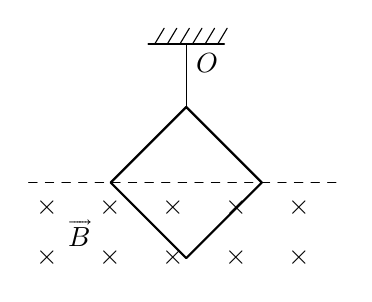
\begin{tikzpicture}[line join=round, line cap=round, >=stealth, scale = 0.8]
            % 1. Vẽ giá treo (trần nhà)
            \draw[thick] (-0.6, 3.5) -- (0.6, 3.5);
            \foreach \x in {-0.5, -0.3, ..., 0.5}
                \draw (\x, 3.5) -- (\x+0.15, 3.75);

            % 2. Vẽ dây treo và điểm O
            \draw (0, 3.5) -- (0, 2.5);
            \node[right] at (0, 3.2) {$O$};

            % 3. Vẽ khung dây hình vuông (xoay 45 độ thành hình thoi)
            % Các đỉnh: Trên (0,2.5), Phải (1.2, 1.3), Dưới (0, 0.1), Trái (-1.2, 1.3)
            \draw[thick] (0, 2.5) -- (1.2, 1.3) -- (0, 0.1) -- (-1.2, 1.3) -- cycle;

            % 4. Vẽ đường biên từ trường (đường đứt nét)
            \draw[dashed] (-2.5, 1.3) -- (2.5, 1.3);

            % 5. Vẽ các ký hiệu từ trường B (dấu X)
            \foreach \x in {-2.2, -1.2, ..., 2.2} {
                \foreach \y in {0.9, 0.1} {
                    \node[] at (\x, \y) {$\times$};
                }
            }
            
            % Nhãn vectơ B
            \node at (-1.7, 0.5) {$\overrightarrow{B}$};

        \end{tikzpicture}
    }
    \choiceTF[1]
    {Cường độ dòng điện trong khung dây luôn có độ lớn là ${\frac{Ba^2}{r \Delta t}}$}
    {\True Dòng điện cảm ứng trong khung dây luôn có chiều ngược chiều kim đồng hồ}
    {Lực từ tổng hợp tác dụng lên khung dây luôn bằng ${0}$}
    {Lực căng dây có độ lớn nhỏ hơn ${mg}$ và không thay đổi}
    \loigiai{
        \begin{itemchoice}
        \itemch ${e = \left| \frac{\Delta \Phi}{\Delta t} \right| = \left| \frac{\Delta B S}{\Delta t} \right| = \frac{(2B - B) \cdot \dfrac{a^2}{2}}{\Delta t} = \frac{Ba^2}{2\Delta t}}$. ${i = \frac{e}{r} = \frac{Ba^2}{2r\Delta t}}$
        \itemch ${B}$ tăng ${\Rightarrow}$ từ thông tăng ${\Rightarrow \overrightarrow{B}_{cu} \uparrow \downarrow \overrightarrow{B} \Rightarrow \overrightarrow{B}_{cu}}$ hướng ra ngoài. Áp dụng quy tắc nắm tay phải được dòng điện cảm ứng trong khung dây có chiều ngược chiều kim đồng hồ
        \itemch Áp dụng quy tắc bàn tay trái được lực từ hướng lên
        \itemch ${T = mg - F_t}$ với ${F_t}$ thay đổi do ${B}$ thay đổi
        \end{itemchoice}
    }
\end{ex}


% Câu 3
\begin{ex}
    \immini[thm]{
        Hình bên là đồ thị biểu diễn sự thay đổi nhiệt độ theo thời gian của một vật có khối lượng ${500 \, \mathrm{g}}$ ban đầu ở thể lỏng tỏa nhiệt đều theo thời gian để đông đặc thành chất rắn. Biết nhiệt dung riêng của vật khi ở thể lỏng là ${3200 \, \mathrm{J/(kg \cdot K)}}$.
        \choiceTF[1]
        {Nhiệt độ nóng chảy của vật khi ở thể rắn là ${0^\circ\mathrm{C}}$}
        {Từ ${\tau = 10}$ phút đến ${\tau = 25}$ phút, vật chỉ tồn tại ở thể rắn}
        {Nhiệt lượng vật tỏa ra trong quá trình đông đặc là ${3200 \, \mathrm{J}}$}
        {\True Nhiệt dung riêng của vật khi ở thể rắn là ${1600 \, \mathrm{J/(kg \cdot K)}}$}
    }{
        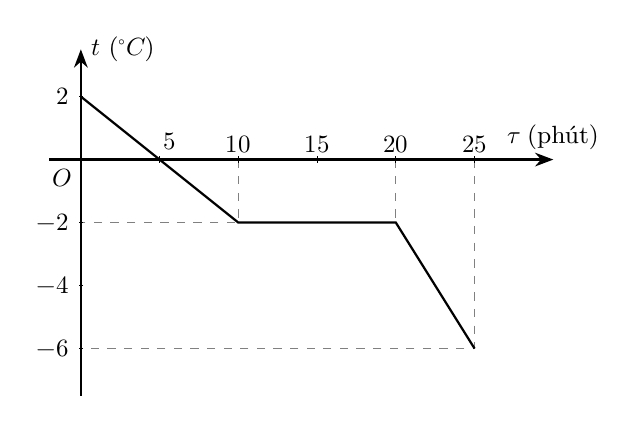
\begin{tikzpicture}[x=0.25cm, y=0.5cm, >={Stealth}, font=\small, scale = 0.8]
            % Vẽ các đường dóng (dashed lines) trước để nằm dưới đồ thị
            \draw[dashed, thin, gray] (10,0) -- (10,-2) -- (0,-2);
            \draw[dashed, thin, gray] (20,0) -- (20,-2);
            \draw[dashed, thin, gray] (25,0) -- (25,-6) -- (0,-6);

            % Trục tọa độ
            \draw[->, thick] (-2, 0) -- (30, 0) node[above] {$\tau$ (phút)};
            \draw[->, thick] (0, -7.5) -- (0, 3.5) node[right] {$t$ ($^\circ C$)};
            
            % Gốc tọa độ O
            \node[below left] at (0,0) {$O$};

            % Các vạch chia và số trên trục tung (y)
            \foreach \y in {-6, -4, -2, 2} {
                \draw (0.15, \y) -- (-0.15, \y) node[left] {${\y}$};
            }

            % Các vạch chia và số trên trục hoành (x)
            \node[above right, xshift=-2pt] at (5, 0) {$5$};
            \draw (5, 0.1) -- (5, -0.1);
            
            \foreach \x in {10, 15, 20, 25} {
                \draw (\x, 0.1) -- (\x, -0.1) node[above] {${\x}$};
            }

            % Đường đồ thị chính
            \draw[thick] (0,2) -- (10,-2) -- (20,-2) -- (25,-6);

        \end{tikzpicture}
    }
        \loigiai{
        \begin{itemchoice}
        \itemch Nhiệt độ nóng chảy của vật khi ở thể rắn là ${-2^\circ\mathrm{C}}$
        \itemch Từ ${\tau = 10}$ phút đến ${\tau = 20}$ phút, vật tồn tại ở cả thể rắn và thể lỏng
        \itemch Trong ${10}$ phút thì ${Q = mc_l \Delta t_l = 0{,}5 \cdot 3200 \cdot (2 + 2) = 6400 \, \mathrm{J}}$
        \itemch Trong ${5}$ phút thì ${\frac{Q}{2} = mc_r \Delta t_r \Rightarrow \frac{6400}{2} = 0{,}5 \cdot c_r \cdot (6 - 2) \Rightarrow 1600 \, \mathrm{J/kgK}}$
        \end{itemchoice}
    }
\end{ex}


% Câu 4
\begin{ex}
    \immini[thm]{
        Như hình vẽ, một xilanh được đặt thẳng đứng có chiều cao ${H = 2 \, \mathrm{m}}$ và tiết diện ${S = 20 \, \mathrm{cm^2}}$, chứa một lượng khí lí tưởng nhất định bên trong. Một piston mỏng, nhẵn, khối lượng không đáng kể chia không gian bên trong xilanh thành hai phần $A$ và B. Piston được nối với đỉnh xilanh bằng một lò xo nhẹ. Ban đầu, piston đứng yên ở chính giữa xilanh, và lò xo có chiều dài tự nhiên, áp suất của khí trong phần $A$ là ${p_A = 2 \cdot 10^4 \, \mathrm{Pa}}$. Bây giờ, khí trong phần $B$ được làm nóng từ từ (nhiệt độ khí trong phần $A$ được giữ không đổi). Khi piston đi lên đoạn ${0{,}5 \, \mathrm{m}}$ thì nhiệt độ nhiệt động của khí trong phần $B$ gấp ${6}$ lần giá trị ban đầu của nó. Lấy ${g = 10 \, \mathrm{m/s^2}}$.
    }{
        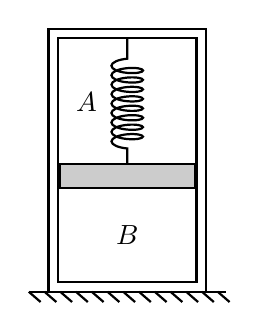
\begin{tikzpicture}[>=latex, thick]
            % Ceiling with hatching
            \draw[thick] (-1.25, 0.28) -- (1.25, 0.28);
            \foreach \x in {-1.25,-1.05,...,1.25}
                \draw (\x, 0.28) -- (\x+0.15, 0.15);
            
            % Spring
            \draw [decoration={coil, aspect=0.3, segment length=1.2mm, amplitude=2mm, pre length=2mm, post length=2mm}, decorate, thick] (0, 1.9) -- (0, 3.5) node[midway,left=0.25cm]{$A$}; 
            
            % Shaded piston
            \draw[fill=gray!40] (-0.86, 1.6) rectangle (0.86, 1.9);
            
            % Cylinder walls
            \draw[thick] (-0.88, 0.4) rectangle (0.88, 3.5);
            \draw[thick] (-1, 0.28) rectangle (1, 3.62);
            \node[] at (0, 1) {$B$};    
        \end{tikzpicture}
    }
    \choiceTF[1]
    {\True Áp suất khí trong phần $B$ ban đầu là ${p_B = 2 \cdot 10^4 \, \mathrm{Pa}}$}
    {\True Áp suất khí trong phần $A$ lúc sau là ${p'_A = 4 \cdot 10^4 \, \mathrm{Pa}}$}
    {\True Áp suất khí trong phần $B$ lúc sau là ${p'_B = 8 \cdot 10^4 \, \mathrm{Pa}}$}
    {Độ cứng lò xo là ${k = 1200 \, \mathrm{N/m}}$}
    \loigiai{
        \begin{itemchoice}
        \itemch Ban đầu ${p_B = p_A = 2 \cdot 10^4 \, \mathrm{Pa}}$
        \itemch $A$ đẳng nhiệt ${\Rightarrow p_A V_A = p'_A V'_A \Rightarrow p_A \cdot S \cdot \frac{H}{2} = p'_A \cdot S \cdot \left( \frac{H}{2} - \Delta l \right)}$ \\${\Rightarrow 2 \cdot 10^4 \cdot \frac{2}{2} = p'_A \cdot \left( \frac{2}{2} - 0{,}5 \right) \Rightarrow p'_A = 4 \cdot 10^4 \, \mathrm{Pa}}$
        \itemch ${\frac{p_B V_B}{T_B} = \frac{p'_B V'_B}{T'_B} \Rightarrow \frac{p_B \cdot S \cdot \dfrac{H}{2}}{T_B} = \frac{p'_B \cdot S \cdot \left( \dfrac{H}{2} + \Delta l \right)}{6T_B}}$ \\
        ${\Rightarrow 2 \cdot 10^4 \cdot \frac{\dfrac{2}{2}}{1} = \frac{p'_B \cdot \left( \dfrac{2}{2} + 0{,}5 \right)}{6} \Rightarrow p'_B = 8 \cdot 10^4 \, \mathrm{Pa}}$
        \itemch ${p'_B = p'_A + \frac{k \Delta l}{S} \Rightarrow 8 \cdot 10^4 = 4 \cdot 10^4 + \frac{k \cdot 0{,}5}{20 \cdot 10^{-4}} \Rightarrow k = 160 \, \mathrm{N/m}}$
        \end{itemchoice}
    }
\end{ex}


% Câu 1
\begin{ex}
    Một nơi có nhiệt độ ${-10^\circ\mathrm{C}}$, thì ở thang Fahrenheit nhiệt độ này bằng bao nhiêu ${^\circ\mathrm{F}}$?
    \shortans{14}
    \loigiai{
        ${t_F = 32 + 1{,}8 t_C = 32 - 1{,}8 \cdot 10 = 14 (^\circ\mathrm{F})}$
    }
\end{ex}


% Câu 2
\begin{ex}
    Một bình chứa một một chất khí lí tưởng được nén ở nhiệt độ ${27^\circ\mathrm{C}}$ và áp suất ${16 \, \mathrm{atm}}$. Nếu nhiệt độ của khí giảm xuống còn ${12^\circ\mathrm{C}}$ và một nửa lượng khí thoát ra khỏi bình thì áp suất khí còn lại trong bình bằng bao nhiêu $\mathrm{atm}$ (làm tròn kết quả đến chữ số hàng phần mười)?
    \shortans{7{,}6}
    \loigiai{
        ${pV = nRT \Rightarrow \frac{p_2}{p_1} = \frac{n_2}{n_1} \cdot \frac{T_2}{T_1} \Rightarrow \frac{p_2}{16} = \frac{1}{2} \cdot \frac{12 + 273}{27 + 273} \Rightarrow p_2 = 7{,}6 \, \mathrm{atm}}$
    }
\end{ex}


% Câu 3
\begin{ex}
    Cho phản ứng hạt nhân: ${_{1}^{2}\mathrm{H} + {}_{1}^{3}\mathrm{H} \to {}_{2}^{4}\mathrm{He} + X}$ tỏa ${17{,}7 \, \mathrm{MeV}}$. Biết độ hụt khối của ${_{1}^{3}\mathrm{H}}$ lớn hơn độ hụt khối của ${_{1}^{2}\mathrm{H}}$ một lượng là ${6{,}3 \cdot 10^{-3} \, \mathrm{u}}$. Phản ứng hạt nhân ${_{1}^{2}\mathrm{H} + {}_{1}^{2}\mathrm{H} \to {}_{2}^{4}\mathrm{He}}$ tỏa ra năng lượng là bao nhiêu MeV (làm tròn kết quả đến chữ số hàng phần mười)?
    \shortans{23{,}6}
    \loigiai{
        ${_{1}^{2}\mathrm{H} + {}_{1}^{3}\mathrm{H} \to {}_{2}^{4}\mathrm{He} + {}_{0}^{1}\mathrm{n}}$\\
        ${\Delta E_1 = (\Delta m_{\mathrm{He}} - \Delta m_{\mathrm{H2}} - \Delta m_{\mathrm{H3}})c^2 \Rightarrow 17{,}7 = (\Delta m_{\mathrm{He}} - \Delta m_{\mathrm{H2}} - \Delta m_{\mathrm{H3}}) \cdot 931{,}5}$\\
        ${\Rightarrow \Delta m_{\mathrm{He}} - \Delta m_{\mathrm{H2}} - \Delta m_{\mathrm{H3}} = \frac{59}{3105} \, \mathrm{u}}$ kết hợp với ${\Delta m_{\mathrm{H3}} - \Delta m_{\mathrm{H2}} = 6{,}3 \cdot 10^{-3} \, \mathrm{u}}$\\
        ${\Delta E_2 = (\Delta m_{\mathrm{He}} - 2\Delta m_{\mathrm{H2}})c^2 = \left( \frac{59}{3105} + 6{,}3 \cdot 10^{-3} \right) \cdot 931{,}5 \approx 23{,}6 \, \mathrm{MeV}}$
    }
\end{ex}


% Câu 4
\begin{ex}
    Đổ một cốc nước nóng vào một bình chứa nước lạnh thì nhiệt độ của nước trong bình tăng thêm ${5^\circ\mathrm{C}}$. Tiếp tục đổ một cốc nước nóng giống ở trên vào bình thì nhiệt độ của nước trong bình tăng thêm ${3^\circ\mathrm{C}}$. Tỉ số giữa khối lượng nước trong một cốc nước nóng với khối lượng nước trong bình nước lạnh ban đầu là bao nhiêu (làm tròn kết quả đến chữ số hàng phần trăm)?
    \shortans{0{,}33}
    \loigiai{
        Gọi nhiệt độ của nước lạnh ban đầu là ${t_l}$\\
        Nhiệt độ cân bằng là ${t_l + 5 \Rightarrow m_n c (t_n - t_l - 5) = m_l c \Delta t_1 \Rightarrow m_n (t_n - t_l - 5) = m_l \cdot 5}$ (1)\\
        Nhiệt độ cân bằng là ${t_l + 8 \Rightarrow 2m_n c (t_n - t_l - 8) = m_l c \Delta t_2 \Rightarrow 2m_n (t_n - t_l - 8) = m_l \cdot 8}$ (2)\\
        Từ (1) và (2) ${\Rightarrow \frac{m_n}{m_l} = \frac{5}{t_n - t_l - 5} = \frac{8}{2(t_n - t_l - 8)} \Rightarrow t_n - t = 20 \Rightarrow \frac{m_n}{m_l} = \frac{1}{3} \approx 0{,}33}$
    }
\end{ex}


% Câu 5
\begin{ex}
    Polonium ${_{84}^{210}\mathrm{Po}}$ là một chất phóng xạ ${\alpha}$ biến đổi thành hạt nhân chì ${_{82}^{206}\mathrm{Pb}}$ với chu kì bán rã ${138}$ ngày. Ban đầu ${(t = 0)}$, một mẫu chất có khối lượng ${90{,}0 \, \mathrm{g}}$, trong đó polonium ${_{84}^{210}\mathrm{Po}}$ chiếm ${30\%}$ khối lượng của mẫu, phần còn lại không có tính phóng xạ. Giả sử toàn bộ các hạt ${\alpha}$ sinh ra trong quá trình phóng xạ đều thoát ra khỏi mẫu. Khối lượng mẫu chất còn lại sau ${276}$ ngày (kể từ ${t = 0}$) là bao nhiêu $\mathrm{g}$? (làm tròn kết quả đến chữ số hàng phần mười).
    \shortans{89{,}6}
    \loigiai{
        ${m_0 = 0{,}3 m_{\mathrm{mẫu}} = 0{,}3 \cdot 90 = 27 \, \mathrm{g}}$\\
        ${m_{\alpha} = m_0 \cdot \frac{A_{\alpha}}{A_{\mathrm{Po}}} \cdot \left( 1 - 2^{-\frac{t}{T}} \right) = 27 \cdot \frac{4}{210} \cdot \left( 1 - 2^{-\frac{276}{138}} \right) \approx 0{,}4 \, \mathrm{g}}$\\
        ${m = m_{\mathrm{mẫu}} - m_{\alpha} = 90 - 0{,}4 = 89{,}6 \, \mathrm{g}}$
    }
\end{ex}


% Câu 6
\begin{ex}
    \immini[thm]{
        Như hình vẽ, một khối khí lí tưởng nhất định được đựng trong một xilanh dẫn nhiệt tốt có khối lượng ${1 \, \mathrm{kg}}$, piston nhẹ có tiết diện ${10 \, \mathrm{cm^2}}$, lò xo nhẹ có độ cứng ${200 \, \mathrm{N/m}}$ nối piston và trần nhà. Ban đầu, nhiệt độ bên ngoài là ${300 \, \mathrm{K}}$, xilanh được đặt trên bàn nằm ngang và lò xo có chiều dài tự nhiên, khoảng cách giữa piston và đáy xilanh là ${0{,}1 \, \mathrm{m}}$. Biết gia tốc trọng trường là ${g = 10 \, \mathrm{m/s^2}}$ và áp suất khí quyển là ${10^5 \, \mathrm{Pa}}$. Bỏ qua mọi ma sát. Giảm từ từ nhiệt độ môi trường xung quanh để xilanh bắt đầu rời khỏi mặt bàn nằm ngang. Lúc này, nhiệt độ của môi trường là bao nhiêu $\mathrm{K}$?
    }{
        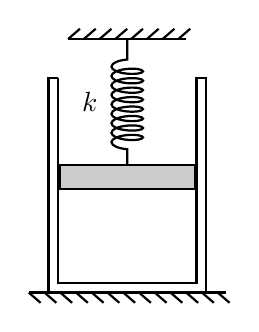
\begin{tikzpicture}[>=latex, thick]
            % Ceiling with hatching
            \draw[thick] (-1.25, 0.28) -- (1.25, 0.28);
            \foreach \x in {-1.25,-1.05,...,1.25}
                \draw (\x, 0.28) -- (\x+0.15, 0.15);
            % Ceiling with hatching
            \draw[thick] (-0.75, 3.5) -- (0.75, 3.5);
            \foreach \x in {-0.75,-0.55,...,0.75}
                \draw (\x, 3.5) -- (\x+0.15, 3.63);
            
            % Spring
            \draw [decoration={coil, aspect=0.3, segment length=1.2mm, amplitude=2mm, pre length=2mm, post length=2mm}, decorate, thick] (0, 1.9) -- (0, 3.5) node[midway,left=0.25cm]{$k$}; 
            
            % Shaded piston
            \draw[fill=gray!40] (-0.86, 1.6) rectangle (0.86, 1.9);
            
            % Cylinder walls (U-shaped container)
            \draw[thick] (-0.88, 3.0) -- (-0.88, 0.4) -- (0.88, 0.4) -- (0.88, 3.0) -- (1.0, 3.0) -- (1.0, 0.28) -- (-1.0, 0.28) -- (-1.0, 3.0) -- (-0.88, 3.0);
        \end{tikzpicture}
    }
    \shortans{135}
    \loigiai{
        Xilanh cân bằng ${pS + m_{xl}g = p_0 S \Rightarrow p = p_0 - \frac{m_{xl}g}{S} = 10^5 - \frac{1 \cdot 10}{10 \cdot 10^{-4}} = 9 \cdot 10^4 \, \mathrm{Pa}}$\\
        Piston cân bằng ${pS + k\Delta l = p_0 S \Rightarrow 9 \cdot 10^4 \cdot 10 \cdot 10^{-4} + 200 \cdot \Delta l = 10^5 \cdot 10 \cdot 10^{-4} \Rightarrow \Delta l = 0{,}05 \, \mathrm{m}}$\\
        ${\frac{pV}{T} = \text{const} \Rightarrow \frac{10^5 \cdot 10 \cdot 10^{-4} \cdot 0{,}1}{300} = \frac{9 \cdot 10^4 \cdot 10 \cdot 10^{-4} \cdot (0{,}1 - 0{,}05)}{T} \Rightarrow T = 135 \, \mathrm{K}}$
    }
\end{ex}

% Câu 1
\begin{ex}
    Các ngành ...(1)... như công nghiệp năng lượng hạt nhân, sản xuất vật liệu...(2)... có nhiều ứng dụng trong nghiên cứu khoa học, y học, sản xuất và đời sống. Điền các cụm từ thích hợp vào các chỗ trống.
    \choice
    {(1) sản xuất hạt nhân; (2) phóng xạ}
    {\True (1) công nghiệp hạt nhân; (2) phóng xạ}
    {(1) công nghiệp hạt nhân; (2) phân hạch}
    {(1) sản xuất hạt nhân; (2) phân hạch}
    \loigiai{}
\end{ex}


% Câu 2
\begin{ex}
    Ngành công nghiệp năng lượng hạt nhân khai thác và sử dụng...(1)... giải phóng thông qua các...(2)... với nhiều mục đích khác nhau như sản xuất điện, tạo lực đẩy cho các phương tiện có công suất lớn (tên lửa, tàu ngầm, tàu phá băng,...) di chuyển. Điền các cụm từ thích hợp vào các chỗ trống.
    \choice
    {(1) năng lượng nguyên tử; (2) phản ứng phân rã}
    {(1) năng lượng hạt nhân; (2) phản ứng phân rã}
    {\True (1) năng lượng hạt nhân; (2) phản ứng phân hạch}
    {(1) năng lượng nguyên tử; (2) phản ứng phân hạch}
    \loigiai{}
\end{ex}


% Câu 3
\begin{ex}
    Nguyên tắc sử dụng năng lượng hạt nhân là
    \choice
    {năng lượng từ phản ứng hạt nhân là động năng làm quay tua bin máy phát điện}
    {năng lượng từ phản ứng hạt nhân là điện năng được sử dụng trực tiếp trong sinh hoạt và sản xuất}
    {năng lượng từ phản ứng hạt nhân là hóa năng được tích trữ trong các ăcquy}
    {\True năng lượng từ phản ứng hạt nhân làm nóng nước để tạo thành hơi nước quay tua bin máy phát điện hoặc tạo lực đẩy}
    \loigiai{}
\end{ex}


% Câu 4
\begin{ex}
    Trong các nhà máy điện nguyên tử hoạt động bình thường hiện nay, phản ứng nào có thể xảy ra trong lò phản ứng hạt nhân của nhà máy để cung cấp năng lượng cho nhà máy hoạt động?
    \choice
    {Phản ứng phân hạch dây chuyền không điều khiển được}
    {Phản ứng nhiệt hạch có kiểm soát}
    {\True Phản ứng phân hạch dây chuyền được khống chế ở mức tới hạn}
    {Phản ứng phân hạch dây chuyền được khống chế ở mức dưới hạn}
    \loigiai{}
\end{ex}


% Câu 5
\begin{ex}
    Nhiên liệu phân hạch trong phần lớn các lò phản ứng hiện nay là
    \choice
    {\True ${}^{235}\mathrm{U}$ và ${}^{239}\mathrm{Pu}$}
    {${}^{235}\mathrm{U}$ và ${}^{238}\mathrm{Pu}$}
    {${}^{238}\mathrm{U}$ và ${}^{239}\mathrm{Pu}$}
    {${}^{238}\mathrm{U}$ và ${}^{238}\mathrm{Pu}$}
    \loigiai{}
\end{ex}


% Câu 6
\begin{ex}
    Trong lò phản ứng hạt nhân, nhiên liệu hạt nhân trải qua phản ứng phân hạch để giải phóng năng lượng hạt nhân. Mô tả nào sau đây về lò phản ứng hạt nhân là đúng?
    \choice
    {Nhiên liệu hạt nhân trong lò phản ứng có thể là ${}_{1}^{2}\mathrm{D}$ hoặc ${}_{1}^{3}\mathrm{T}$}
    {\True Trong lò phản ứng hạt nhân xảy ra phản ứng dây chuyền}
    {Tổng năng lượng liên kết của các hạt nhân mới sau phản ứng nhỏ hơn năng lượng liên kết của hạt nhân trước phản ứng}
    {Trong lò phản ứng hạt nhân, neutron chậm có thể được chuyển thành neutron nhanh thông qua than chì hoặc nước nặng}
    \loigiai{}
\end{ex}


% Câu 7
\begin{ex}
    Chất thải hạt nhân trong các lò phản ứng hạt nhân có độ phóng xạ cao. Phương pháp xử lý thông dụng hiện nay là cho chúng vào các thùng chứa đặc biệt và sau đó
    \choice
    {thả xuống đáy biển}
    {đưa vào sa mạc}
    {vận chuyển lên mặt trăng}
    {\True chôn sâu dưới lòng đất}
    \loigiai{}
\end{ex}


% Câu 8
\begin{ex}
    Vai trò của các nhà máy điện hạt nhân trong đời sống:
    (1) giúp giảm khí thải nhà kính;
    (2) mang lại nguồn cung cấp điện ổn định;
    (3) đảm bảo năng lượng bền vững;
    (4) đem lại lợi ích kinh tế lâu dài.
    Trong 4 ý trên số ý đúng là
    \choice
    {1}
    {2}
    {3}
    {\True 4}
    \loigiai{}
\end{ex}


% Câu 9
\begin{ex}
    Một trong những hướng con người đã nghiên cứu để tạo nguồn năng lượng nhân tạo to lớn cho mục đích hòa bình là
    \choice
    {Năng lượng mặt trời}
    {Năng lượng thủy điện}
    {Năng lượng gió}
    {\True Năng lượng hạt nhân}
    \loigiai{}
\end{ex}


% Câu 10
\begin{ex}
    Thiết bị chụp cắt lớp phát xạ positron có tên gọi là gì
    \choice
    {X quang}
    {CT}
    {SPECT}
    {\True PET}
    \loigiai{}
\end{ex}


% Câu 11
\begin{ex}
    Nguyên lý của chụp cắt lớp vi tính phát xạ positron (PET) là: Các đồng vị phóng xạ ${}_{8}^{15}\mathrm{O}$ được tiêm vào cơ thể con người, positron được giải phóng do ${}_{8}^{15}\mathrm{O}$ phân rã gặp electron trong cơ thể thì hủy nhau và chuyển hóa thành một cặp photon gamma - được máy dò phát hiện. Sau khi thu thập, hình ảnh rõ nét được tạo ra thông qua xử lí máy tính. Phát biểu nào sau đây là sai?
    \choice
    {Phương trình phân rã của ${}_{8}^{15}\mathrm{O}$ trong cơ thể con người là ${}_{8}^{15}\mathrm{O} \rightarrow {}_{7}^{15}\mathrm{N} + {}_{1}^{0}\mathrm{e}^{+}$}
    {Phương trình hủy diệt của các positron và electron là ${}_{1}^{0}\mathrm{e}^{+} + {}_{-1}^{0}\mathrm{e}^{-} \rightarrow 2\gamma$}
    {Trong PET, công dụng chính của ${}_{8}^{15}\mathrm{O}$ là làm nguyên tử đánh dấu}
    {\True Trong PET, mục đích chính là tham gia vào quá trình trao đổi chất của cơ thể con người}
    \loigiai{}
\end{ex}


% Câu 12
\begin{ex}
    Xạ trị trong y học để trị bệnh ung thư là ứng dụng của vật lí khi nghiên cứu
    \choice
    {sóng điện từ}
    {chuyển động}
    {\True phản ứng hạt nhân}
    {vật liệu bán dẫn}
    \loigiai{}
\end{ex}


% Câu 13
\begin{ex}
    Trong điều trị bệnh ung thư, để diệt các tế bào khối u, người ta thường dùng
    \choice
    {cosixin}
    {chất 5BU}
    {\True tia phóng xạ hoặc hóa chất}
    {EMS}
    \loigiai{}
\end{ex}


% Câu 14
\begin{ex}
    Vai trò của y học hạt nhân trong đời sống:
    (1) Chẩn đoán và điều trị các bệnh ung thư, bệnh nội tiết, tim mạch.
    (2) Xử lí thực phẩm sử dụng bức xạ ion hoá, khử trùng các sản phẩm và thiết bị y tế (đồng phục, cụ, băng gạc...);
    (3) Xác định nguồn nước, đánh giá nguy cơ xâm nhập nước mặn hoặc ô nhiễm nguồn nước, kiểm tra khả năng sử dụng nước;
    (4) Phát hiện các khu vực đất bị xói mòn.
    Trong 4 ý trên số ý đúng là
    \choice
    {1}
    {2}
    {3}
    {\True 4}
    \loigiai{}
\end{ex}


% Câu 15
\begin{ex}
    Chất phóng xạ được ứng dụng rộng rãi trong nông nghiệp là
    \choice
    {Chuẩn đoán hình ảnh và điều trị ung thư}
    {\True Tạo đột biến cải thiện giống cây trồng}
    {Phát hiện các khiếm khuyết trong vật liệu}
    {Xác định tuổi của các mẫu vật}
    \loigiai{}
\end{ex}


% Câu 16
\begin{ex}
    Nêu một số ứng dụng của chất phóng xạ trong đời sống?
    \choice
    {sử dụng trong y học để chuẩn đoán hình ảnh và điều trị ung thư}
    {sử dụng trong nông nghiệp để tạo đột biến cải thiện giống cây trồng}
    {sử dụng trong công nghiệp để phát hiện các khiếm khuyết trong vật liệu, sử dụng trong khảo cổ để xác định tuổi của các mẫu vật}
    {\True Cả A, B và C}
    \loigiai{}
\end{ex}


% Câu 17
\begin{ex}
    Đâu không phải là ứng dụng của chất phóng xạ?
    \choice
    {Chiếu xạ các nguyên tố phóng xạ để điều trị khối u ác tính}
    {Đồng vị phóng xạ làm nguyên tử đánh dấu}
    {\True Nguồn phóng xạ được cất giữ cách xa thực phẩm, nguồn nước và môi trường sống}
    {Khảo cổ học phân tích nguyên tố phóng xạ}
    \loigiai{}
\end{ex}


% Câu 18
\begin{ex}
    Một hạt nhân nặng có số khối ${234}$ có năng lượng liên kết riêng bằng ${7{,}6 \, \mathrm{MeV/nucleon}}$ phân hạch thành các hạt nhân nhẹ có năng lượng liên kết riêng xấp xỉ bằng nhau và bằng ${8{,}5 \, \mathrm{MeV/nucleon}}$. Khi một phân hạch xảy ra một phần năng lượng liên kết sẽ được giải phóng. Phần năng lượng đó là
    \choice
    {${203 \, \mathrm{MeV}}$}
    {\True ${211 \, \mathrm{MeV}}$}
    {${180 \, \mathrm{MeV}}$}
    {${190 \, \mathrm{MeV}}$}
    \loigiai{
        $\Delta E = W_{lks} - W_{lkt} = 234 \cdot \left( 8{,}5 - 7{,}6 \right) = 210{,}6 \, \mathrm{MeV}$
    }
\end{ex}


% Câu 1
\begin{ex}
    Các nội dung sau đề cập đến nhà máy điện hạt nhân.
    \choiceTF[1]
    {\True Để kiểm soát năng lượng toả ra từ lò phản ứng, người ta dùng các thanh điều khiển có chứa boron hay cadmium}
    {\True Các thanh điều khiển có vai trò hấp thụ neutron để đảm bảo duy trì được phản ứng phân hạch dây chuyền có kiểm soát}
    {\True Năng lượng toả ra từ lò phản ứng hạt nhân dùng để biến nước thành hơi ở áp suất cao và làm quay tuabin của máy phát điện}
    {Các thanh nhiên liệu sau khi sử dụng được đưa lại nơi sản xuất để tái sử dụng}
    \loigiai{
        \begin{itemchoice}
        \itemch 
        \itemch 
        \itemch 
        \itemch Các thanh nhiên liệu sau khi sử dụng được đưa lại nơi sản xuất để tái sử dụng ngay.
        \end{itemchoice}
    }
\end{ex}


% Câu 2
\begin{ex}
    Các nội dung sau đề cập đến các ưu điểm, nhược điểm và cơ hội phát triển của các nhà máy điện hạt nhân.
    \choiceTF[1]
    {\True Ưu điểm của nhà máy điện hạt nhân: cung cấp năng lượng hạt nhân giúp giảm khí thải nhà kính, mang lại nguồn cung cấp điện ổn định, đảm bảo năng lượng bền vững, đem lại lợi ích kinh tế lâu dài. Hệ thống khai thác năng lượng hạt nhân có thể hoạt động trong thời gian dài mà không cần bổ sung nhiên liệu}
    {\True Nhược điểm của nhà máy điện hạt nhân: tạo ra chất thải nguy hại cho môi trường, quá trình vận hành có khả năng rủi ro và sự cố khá cao, chi phí xây dựng tốn kém cũng như tiềm tàng nguy cơ về an ninh hạt nhân}
    {\True Để đáp ứng nhu cầu năng lượng không ngừng tăng nhanh thì cơ hội phát triển các nhà máy điện hạt nhân là khả thi}
    {Việt Nam đã có nhà máy điện hạt nhân hòa vào lưới điện quốc gia}
    \loigiai{
        \begin{itemchoice}
        \itemch 
        \itemch 
        \itemch 
        \itemch Chưa có
        \end{itemchoice}
    }
\end{ex}


% Câu 3
\begin{ex}
    \immini[thm]{
        Hình vẽ dưới đây là sơ đồ của một lò phản ứng hạt nhân.
        \choiceTF[1]
        {\True Thanh uranium là nhiên liệu hạt nhân và vật liệu cốt lõi là ${}^{235}\mathrm{U}$}
        {Than chì hấp thụ neutron}
        {Thanh cadmium đóng vai trò làm chậm neutron}
        {\True Chức năng của lớp xi măng bảo vệ là chặn tia gamma và tránh nguy cơ phóng xạ}
    }{
        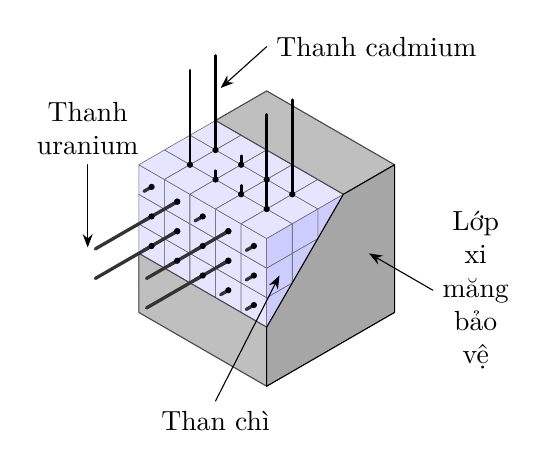
\begin{tikzpicture}[
            scale = 0.75, >={Stealth},
            x={(-150:0.5cm)}, y={(90:0.5cm)}, z={(-30:0.5cm)},
            line join=round, line cap=round,
            block/.style={draw=black!60, fill=blue!10, very thin},
            uranium/.style={draw=black!80, line width=1.2pt},
            cadmium/.style={draw=black, line width=1pt},
            concrete/.style={fill=gray!50, draw=black!70},
            font=\linespread{1}\selectfont
        ]
            % 1. Vẽ các khối Than chì (Core) - Vẽ từ sau ra trước để đúng lớp
            \foreach \z in {0,...,4} {
                \foreach \y in {0,...,4} {
                    \foreach \x in {0,...,4} {
                        % Vẽ các mặt của khối lập phương nhỏ
                        \filldraw[block] (\x+1,\y,\z) -- (\x+1,\y+1,\z) -- (\x+1,\y+1,\z+1) -- (\x+1,\y,\z+1) -- cycle; % Mặt phải
                        \filldraw[block] (\x,\y+1,\z) -- (\x+1,\y+1,\z) -- (\x+1,\y+1,\z+1) -- (\x,\y+1,\z+1) -- cycle; % Mặt trên
                        \filldraw[block, fill=blue!20] (\x,\y,\z+1) -- (\x+1,\y,\z+1) -- (\x+1,\y+1,\z+1) -- (\x,\y+1,\z+1) -- cycle; % Mặt trước
                    }
                }
            }

            % 4. Vẽ Lớp Xi măng bảo vệ (Phần đế và tường bao quanh)
            % Tường trước
            \filldraw[concrete] (5,0,0) -- (5,2,0) -- (5,2,5) -- (5,0,5) -- cycle;
            % Tường trên
            \filldraw[concrete] (0,5,0) -- (2,5,0) -- (2,5,5) -- (0,5,5) -- cycle;
            
            % Phần tường phía trước bị cắt (jagged edge)
            \filldraw[gray!70, draw=black] 
                (0,0,5) -- (5,0,5) -- (5,2,5) -- (2,5,5) -- (0,5,5) -- cycle;


            % 2. Vẽ các Thanh Uranium (Đâm ngang từ phía sau/trái)
            \foreach \y in {3.5, 4.5} {
                \foreach \z in {1.5, 3.5} {
                    \draw[uranium] (5, \y, \z) -- (8.2, \y, \z);
                    \fill (5, \y, \z) circle (1.5pt);
                }
            }
            \foreach \y in {2.5, 3.5, 4.5} {
                \foreach \z in {0.5, 1.5, 2.5, 3.5, 4.5} {
                    \draw[uranium] (5, \y, \z) -- (5.3, \y, \z);
                    \fill (5, \y, \z) circle (1.5pt);
                }
            }

            % 3. Vẽ các Thanh Cadmium (Thẳng đứng từ trên xuống)
            \foreach \x in {3, 4} {
                \foreach \z in {1, 4} {
                    \draw[cadmium] (\x, 5, \z) -- (\x, 8.2, \z);
                    \fill (\x, 5, \z) circle (1.5pt);
                }
            }
            \foreach \x in {3, 4} {
                \foreach \z in {2, 3} {
                    \draw[cadmium] (\x, 5, \z) -- (\x, 5.3, \z);
                    \fill (\x, 5, \z) circle (1.5pt);
                }
            }
            % 5. Chú thích (Labels)
            \begin{scope}[shift={(0,0,0)}]
                % Thanh Cadmium
                \draw[<-] (2.8, 7, 1) -- (1, 7.5, 1) node[right, align=center] {Thanh cadmium};
                
                % Thanh Uranium
                \draw[<-] (8, 4.2, 1) -- (5, 4, -2) node[above, align=center] {Thanh\\uranium};
                
                % Than chì
                \draw[<-] (4.5,3.5,5) -- (6.5, 0, 4.5) node[below] {Than chì};
                
                % Lớp xi măng
                \draw[<-] (1.5,3,5.5) -- (2.5, 4, 9) node[right, align=center] {Lớp\\xi\\măng\\bảo\\vệ};
            \end{scope}

        \end{tikzpicture}
    }
    \loigiai{
        \begin{itemchoice}
        \itemch 
        \itemch Than chì làm chậm neutron
        \itemch Thanh cadmium đóng vai trò hấp thụ neutron
        \itemch 
        \end{itemchoice}
    }
\end{ex}


% Câu 4
\begin{ex}
    Phosphorus ${}_{15}^{32}\mathrm{P}$ là đồng vị phóng xạ $\beta^{-}$ với chu kì bán rã ${14{,}26}$ ngày. Trong phương pháp nguyên tử đánh dấu, các nhà khoa học sử dụng ${}_{15}^{32}\mathrm{P}$ để nghiên cứu sự hấp thụ và vận chuyển phosphorus trong cây trồng. Trong một thí nghiệm, người ta tưới dung dịch nước chứa ${215 \, \mathrm{mg}}$ ${}_{15}^{32}\mathrm{P}$ cho cây khoai tây. Sau đó, ngắt một chiếc lá cây và đo độ phóng xạ của nó được ${4{,}48 \cdot 10^{12} \, \mathrm{Bq}}$. Khối lượng mol tính theo gam bằng số khối hạt nhân đó.
    \choiceTF[1]
    {\True Sản phẩm phân rã của ${}_{15}^{32}\mathrm{P}$ là ${}_{16}^{32}\mathrm{S}$}
    {\True Tại thời điểm đo, lượng ${}_{15}^{32}\mathrm{P}$ trong lá cây bằng ${0{,}2\%}$ lượng ${}_{15}^{32}\mathrm{P}$ ban đầu tưới cho cây}
    {\True Độ phóng xạ của chiếc lá vào thời điểm ${1{,}50}$ ngày sau khi ngắt là ${4{,}16 \cdot 10^{12} \, \mathrm{Bq}}$}
    {\True Số hạt electron chiếc lá đã phóng ra trong ${1{,}50}$ ngày sau khi ngắt là ${5{,}60 \cdot 10^{17}}$ hạt}
    \loigiai{
        \begin{itemchoice}
        \itemch ${}_{15}^{32}\mathrm{P} \rightarrow {}_{16}^{32}\mathrm{S} + {}_{-1}^{0}\mathrm{e}$
        \itemch $H_0 = \lambda N_0 = \frac{\ln 2}{T} \cdot N_0 \Rightarrow 4{,}48 \cdot 10^{12} = \frac{\ln 2}{14{,}26 \cdot 24 \cdot 60 \cdot 60} \cdot N_0 \Rightarrow N_0 \approx 7{,}96 \cdot 10^{18}$ \\
        $n_0 = \frac{N_0}{N_A} = \frac{7{,}96 \cdot 10^{18}}{6{,}02 \cdot 10^{23}} \approx 1{,}322 \cdot 10^{-5} \, \mathrm{mol}$ \\
        $m_0 = n_0 M = 1{,}322 \cdot 10^{-5} \cdot 32 \approx 4{,}23 \cdot 10^{-4} \, \mathrm{g} \approx 0{,}423 \, \mathrm{mg} \Rightarrow \frac{0{,}423}{215} \approx 0{,}2\%$
        \itemch $H = H_0 \cdot 2^{-\frac{t}{T}} = 4{,}48 \cdot 10^{12} \cdot 2^{-\frac{1{,}5}{14{,}26}} \approx 4{,}16 \cdot 10^{12} \, \mathrm{Bq}$
        \itemch $\Delta N = N_0 \left( 1 - 2^{-\frac{t}{T}} \right) = 7{,}96 \cdot 10^{18} \left( 1 - 2^{-\frac{1{,}5}{14{,}26}} \right) \approx 5{,}60 \cdot 10^{17}$
        \end{itemchoice}
    }
\end{ex}


% Câu 1
\begin{ex}
    Một lò phản ứng hạt nhân có công suất ${100 \, \mathrm{MW}}$ và sử dụng nhiên liệu là ${}_{92}^{235}\mathrm{U}$. Coi mỗi hạt nhân ${}_{92}^{235}\mathrm{U}$ phân hạch toả ra năng lượng trung bình là ${200 \, \mathrm{MeV}}$. Trong mỗi giây, số phân hạch trong lò là $z \cdot 10^{18}$. Giá trị của $z$ bằng bao nhiêu (làm tròn kết quả đến chữ số hàng phần mười)?
    \shortans{3{,}1}
    \loigiai{
        $N = \frac{Pt}{\Delta E} = \frac{100 \cdot 10^6}{200 \cdot 1{,}6 \cdot 10^{-13}} \approx 3{,}1 \cdot 10^{18}$
    }
\end{ex}


% Câu 2
\begin{ex}
    Một lò phản ứng phân hạch có công suất ${250 \, \mathrm{kW}}$. Cho rằng toàn bộ năng lượng mà lò phản ứng này sinh ra đều do sự phân hạch của uranium ${}^{235}\mathrm{U}$ và đồng vị này chỉ bị tiêu hao bởi quá trình phân hạch. Coi mỗi năm có ${365}$ ngày; mỗi phân hạch sinh ra trung bình ${175 \, \mathrm{MeV}}$ và khối lượng mol nguyên tử của ${}^{235}\mathrm{U}$ là ${235 \, \mathrm{g/mol}}$. Khối lượng ${}^{235}\mathrm{U}$ mà lò phản ứng tiêu thụ trong ${1{,}5}$ năm là bao nhiêu gam (làm tròn kết quả đến chữ số hàng đơn vị)?
    \shortans{165}
    \loigiai{
        $A = Pt = 250 \cdot 10^3 \cdot 1{,}5 \cdot 365 \cdot 24 \cdot 60 \cdot 60 = 1{,}1826 \cdot 10^{13} \, \mathrm{J}$ \\
        $N = \frac{A}{\Delta E} = \frac{1{,}1826 \cdot 10^{13}}{175 \cdot 1{,}6 \cdot 10^{-13}} \approx 4{,}22 \cdot 10^{23}$ \\
        $n = \frac{N}{N_A} = \frac{4{,}22 \cdot 10^{23}}{6{,}02 \cdot 10^{23}} \approx 0{,}7 \, \mathrm{mol}$ \\
        $m = nM = 0{,}7 \cdot 235 \approx 165 \, \mathrm{g}$
    }
\end{ex}


\begin{ex}
    \sochc{2}{Các nhà khoa học đã xác định được độ phóng xạ của ${1 \, \mathrm{g}}$ mẫu carbon trong cơ thể sinh vật sống là ${0{,}231 \, \mathrm{Bq}}$. Biết rằng, trong số các đồng vị của carbon có trong mẫu, chỉ có ${}_{6}^{14}\mathrm{C}$ là đồng vị phóng xạ với chu kì bán rã là ${5730}$ năm (${1}$ năm = ${365{,}2422}$ ngày).
    }
    % Câu 3
    \begin{chc}
        Số nguyên tử ${}_{6}^{14}\mathrm{C}$ có trong ${1 \, \mathrm{g}}$ mẫu carbon đó là $z \cdot 10^{10}$. Giá trị $z$ bằng bao nhiêu (làm tròn kết quả đến chữ số hàng phần trăm)?
        \shortans{6{,}03}
        \loigiai{
            $H_0 = \lambda N_0 = \frac{\ln 2}{T} \cdot N_0 \Rightarrow 0{,}231 = \frac{\ln 2}{5730 \cdot 365{,}2422 \cdot 24 \cdot 60 \cdot 60} \cdot N_0 \Rightarrow N_0 \approx 6{,}03 \cdot 10^{10}$
        }
    \end{chc}
    % Câu 4
    \begin{chc}
        Vào ngày ${19/9/1991}$, trong khi đang tìm đường vượt qua dãy Otztal Alps, hai nhà leo núi người Đức đã phát hiện thấy xác ướp người cổ được bảo quản hầu như nguyên vẹn trong băng tuyết tại Hauslabjoch, khu vực giữa biên giới Áo và Italia. Xác ướp đó được đặt tên là người băng Otzi. Các nhà khoa học đã đo được độ phóng xạ của ${1 \, \mathrm{g}}$ mẫu carbon trong cơ thể người băng Otzi lúc đó là ${0{,}121 \, \mathrm{Bq}}$. Niên đại của người băng đó là bao nhiêu nghìn năm (làm tròn kết quả đến chữ số hàng phần trăm)?
        \shortans{5{,}35}
        \loigiai{
            $H = H_0 \cdot 2^{-\frac{t}{T}} \Rightarrow 0{,}121 = 0{,}231 \cdot 2^{-\frac{t}{5730}} \Rightarrow t \approx 5{,}35 \cdot 10^3$ năm
        }
    \end{chc}
\end{ex}




% Câu 5
\begin{ex}
    Trong một mẫu đá được các nhà du hành mang về Trái Đất từ Mặt Trăng, các nhà khoa học phát hiện có ${75\%}$ potassium ${}_{19}^{40}\mathrm{K}$ ban đầu đã biến thành argon ${}_{18}^{40}\mathrm{Ar}$. Biết rằng, khi được hình thành, mẫu đá không chứa argon; toàn bộ argon được tạo ra có nguồn gốc từ potassium và không hề bị thất thoát vào môi trường. Cho chu kì bán rã của ${}_{19}^{40}\mathrm{K}$ là ${1{,}25 \cdot 10^9}$ năm. Sau bao nhiêu tỉ năm nữa thì lượng potassium ${}_{19}^{40}\mathrm{K}$ còn lại bằng ${6{,}25\%}$ lượng potassium ${}_{19}^{40}\mathrm{K}$ ban đầu?
    \shortans{2{,}5}
    \loigiai{
        $N = N_0 \cdot 2^{-\frac{t}{T}} \Rightarrow \left\{\begin{aligned} & 1 - \frac{75}{100} = 2^{-\frac{t_1}{1{,}25 \cdot 10^9}} \\ & \frac{6{,}25}{100} = 2^{-\frac{t_2}{1{,}25 \cdot 10^9}} \end{aligned}\right. \Rightarrow \left\{\begin{aligned} & t_1 = 2{,}5 \cdot 10^9 \\ & t_2 = 5 \cdot 10^9 \end{aligned}\right. \, \mathrm{(năm)}$ \\
        $\Delta t = t_2 - t_1 = 5 \cdot 10^9 - 2{,}5 \cdot 10^9 = 2{,}5 \cdot 10^9$ (năm)
    }
\end{ex}


% Câu 6
\begin{ex}
    Tiêm ${10 \, \mathrm{cm^3}}$ dung dịch chứa đồng vị phóng xạ ${}^{24}\mathrm{Na}$ với nồng độ ${10^{-3} \, \mathrm{mol/L}}$ vào tĩnh mạch của người. Sau ${6}$ giờ lấy ${20 \, \mathrm{cm^3}}$ máu của người đó thì thấy có ${2{,}9 \cdot 10^{-8} \, \mathrm{mol}}$ ${}^{24}\mathrm{Na}$ trong đó. Cho chu kì bán rã của ${}^{24}\mathrm{Na}$ là ${15 \, \mathrm{h}}$. Thể tích của máu có trong cơ thể người là bao nhiêu lít (làm tròn kết quả đến chữ số hàng phần mười)?
    \shortans{5{,}2}
    \loigiai{
        $n_0 = C_m V = 10^{-3} \cdot 10 \cdot 10^{-3} = 10^{-5} \, \mathrm{mol}$ \\
        $n = n_0 \cdot 2^{-\frac{t}{T}} = 10^{-5} \cdot 2^{-\frac{6}{15}} \, \mathrm{mol}$ \\
        $\frac{V + 10}{20} = \frac{10^{-5} \cdot 2^{-\frac{6}{15}}}{2{,}9 \cdot 10^{-8}} \Rightarrow V \approx 5{,}2 \cdot 10^3 \, \mathrm{cm^3} = 5{,}2 \, \mathrm{l}$
    }
\end{ex}

% Câu 1
\begin{ex}
    Liên hệ giữa chu kì bán rã ${T}$ và hằng số phóng xạ ${\lambda}$ của một chất phóng xạ là
    \choice
    {${T = \frac{1}{\lambda}}$}
    {${T = \frac{\lambda}{\ln 2}}$}
    {${T = 2\pi\lambda}$}
    {\True ${T = \frac{\ln 2}{\lambda}}$}
    \loigiai{
        Liên hệ giữa chu kì bán rã ${T}$ và hằng số phóng xạ ${\lambda}$ là ${T = \frac{\ln 2}{\lambda}}$
    }
\end{ex}


% Câu 2
\begin{ex}
    Đơn vị khối lượng nguyên tử ${\mathrm{amu}}$ được định nghĩa theo khối lượng của đồng vị
    \choice
    {${^4_2\mathrm{He}}$}
    {\True ${^{12}_6\mathrm{C}}$}
    {${^{14}_7\mathrm{N}}$}
    {${^{210}_{84}\mathrm{Po}}$}
    \loigiai{
        Đơn vị khối lượng nguyên tử ${\mathrm{amu}}$ được định nghĩa bằng ${\frac{1}{12}}$ khối lượng của đồng vị ${^{12}_6\mathrm{C}}$
    }
\end{ex}


% Câu 3
\begin{ex}
    Máy phát điện xoay chiều là thiết bị làm biến đổi
    \choice
    {quang năng thành điện năng}
    {cơ năng thành quang năng}
    {điện năng thành cơ năng}
    {\True cơ năng thành điện năng}
    \loigiai{
        Máy phát điện xoay chiều là thiết bị làm biến đổi cơ năng thành điện năng
    }
\end{ex}


% Câu 4
\begin{ex}
    Một lượng chất lỏng có khối lượng ${m}$ và nhiệt hóa hơi riêng ${L}$. Nhiệt lượng cần cung cấp cho lượng chất lỏng trên hóa hơi hoàn toàn ở nhiệt độ không đổi là ${Q}$. Hệ thức đúng là
    \choice
    {${m = \frac{1}{2}LQ^2}$}
    {\True ${Q = mL}$}
    {${m = QL}$}
    {${Q = \frac{1}{2}mL^2}$}
    \loigiai{
        Nhiệt lượng cần cung cấp để hóa hơi hoàn toàn một lượng chất lỏng ở nhiệt độ không đổi là ${Q = mL}$
    }
\end{ex}


% Câu 5
\begin{ex}
    Một khối khí lí tưởng nhất định có áp suất ${p}$ và nhiệt độ nhiệt động ${T}$. Phát biểu nào sau đây đúng?
    \choice
    {Khi ${p}$ tăng thì mật độ phân tử tăng}
    {Khi ${T}$ giảm thì mật độ phân tử tăng}
    {\True Khi ${\frac{p}{T}}$ tăng thì mật độ phân tử tăng}
    {Khi ${\frac{p}{T}}$ tăng thì mật độ phân tử không đổi}
    \loigiai{
        Ta có: ${p = \mu kT \Rightarrow \mu = \frac{p}{kT} \Rightarrow \mu \sim \frac{p}{T}}$. Vậy khi ${\frac{p}{T}}$ tăng thì mật độ phân tử ${\mu}$ tăng
    }
\end{ex}


% Câu 6
\begin{ex}
    Một lượng chất lỏng nhất định thì
    \choice
    {có thể tích riêng và hình dạng riêng}
    {không có thể tích riêng nhưng có hình dạng riêng}
    {không có thể tích riêng và hình dạng riêng}
    {\True có thể tích riêng nhưng không có hình dạng riêng}
    \loigiai{
        Chất lỏng có thể tích riêng xác định nhưng không có hình dạng riêng mà có hình dạng của bình chứa nó
    }
\end{ex}


% Câu 7
\begin{ex}
    Khi nói về sóng điện từ, phát biểu nào dưới đây sai?
    \choice
    {Sóng điện từ truyền được trong chân không}
    {Sóng điện từ bị phản xạ khi gặp mặt phân cách giữa hai môi trường}
    {Trong chân không, sóng điện từ lan truyền với vận tốc bằng vận tốc ánh sáng}
    {\True Trong sóng điện từ, Vector cường độ điện trường và Vector cảm ứng từ ngược hướng nhau}
    \loigiai{
        Trong sóng điện từ, Vector cường độ điện trường và Vector cảm ứng từ luôn vuông phương với nhau và vuông góc với phương truyền sóng
    }
\end{ex}


% Câu 8
\begin{ex}
\immini[thm]{
    Như hình vẽ, một từ trường đều có đường sức từ thẳng đứng hướng xuống. Đoạn dây dẫn thẳng ${ab}$ mang dòng điện không đổi quay quanh điểm ${a}$ để thay đổi từ vị trí nằm ngang ${1}$ đến vị trí ${2}$ trong mặt phẳng thẳng đứng thì lực từ tác dụng lên đoạn dây
    \choice
    {có hướng không đổi và độ lớn tăng}
    {\True có hướng không đổi và độ lớn giảm}
    {có độ lớn không đổi nhưng hướng thay đổi}
    {có độ lớn thay đổi và hướng thay đổi}
}{
    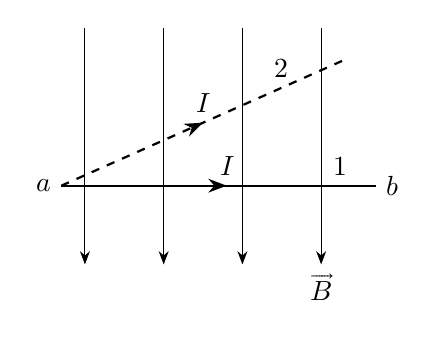
\begin{tikzpicture}[>=Stealth, scale=1]
        % Magnetic field lines
        \foreach \x in {0.5, 1.5, 2.5, 3.5} {
            \draw[->] (\x, 2.5) -- (\x, -0.5);
        }
        \node at (3.5, -0.5) [below] {$\overrightarrow{B}$};

        % Starting point 'a'
        \coordinate (A) at (0.2, 0.5);
        \node at (A) [left] {$a$};

        % Path 1: Horizontal line
        \draw[thick] (A) -- (4.2, 0.5) node[right] {$b$};
        \draw[thick, ->] (1.9, 0.5) -- (2.3, 0.5) node[above] {$I$};
        \node at (3.75, 0.5) [above] {$1$};

        % Path 2: Dotted diagonal line
        \draw[thick, dashed, postaction={decorate, decoration={markings, mark=at position 0.5 with {\arrow{>}, \node[above] {$I$};}}}] (A) -- (3.8, 2.1);
        \node at (3.0, 1.75) [above] {$2$};
    \end{tikzpicture}
}
    \loigiai{
        Áp dụng quy tắc bàn tay trái ${\Rightarrow}$ lực từ có hướng không đổi (hướng ra ngoài mặt phẳng hình vẽ).\\
        Ban đầu góc ${\alpha = 90^\circ}$ sau đó giảm nên lực từ ${F = BIL\sin\alpha}$ có độ lớn giảm
    }
\end{ex}


% Câu 9
\begin{ex}
    Nhiệt độ cơ thể bình thường của một người khoảng
    \choice
    {${273 \, \mathrm{K}}$}
    {\True ${310 \, \mathrm{K}}$}
    {${300 \, \mathrm{K}}$}
    {${315 \, \mathrm{K}}$}
    \loigiai{
        Nhiệt độ cơ thể người bình thường khoảng ${37^\circ\mathrm{C}}$. Đổi sang thang Kelvin: ${T = 37 + 273 = 310 \, \mathrm{K}}$
    }
\end{ex}


% Câu 10
\begin{ex}
    Năm 1934, Joliot-Curie đã bắn phá hạt nhân nhôm ${^{27}_{13}\mathrm{Al}}$ bằng các hạt alpha, tạo ra đồng vị phóng xạ nhân tạo đầu tiên ${X}$ thông qua phản ứng: ${\alpha + ^{27}_{13}\mathrm{Al} \to \mathrm{n} + X}$. Số hiệu nguyên tử và số khối của ${X}$ lần lượt là
    \choice
    {${15}$ và ${28}$}
    {\True ${15}$ và ${30}$}
    {${16}$ và ${30}$}
    {${17}$ và ${31}$}
    \loigiai{
        Phương trình phản ứng: ${^4_2\mathrm{He} + ^{27}_{13}\mathrm{Al} \to ^1_0\mathrm{n} + ^A_Z X}$.\\
        Áp dụng định luật bảo toàn số khối và bảo toàn điện tích:
        ${\left\{\begin{aligned} & 4 + 27 = 1 + A \\ & 2 + 13 = 0 + Z \end{aligned}\right. \Rightarrow \left\{\begin{aligned} & A = 30 \\ & Z = 15 \end{aligned}\right.}$
    }
\end{ex}


% Câu 11
\begin{ex}
    Một lượng khí lí tưởng nhất định có thể tích ${100 \, \mathrm{cm^3}}$ ở ${27^\circ\mathrm{C}}$. Nếu áp suất không đổi và thể tích của khí tăng lên thành ${120 \, \mathrm{cm^3}}$ thì nhiệt độ của khí là
    \choice
    {${-23^\circ\mathrm{C}}$}
    {${22{,}5^\circ\mathrm{C}}$}
    {${32{,}4^\circ\mathrm{C}}$}
    {\True ${87^\circ\mathrm{C}}$}
    \loigiai{
        Quá trình đẳng áp: ${\frac{V}{T} = \mathrm{const} \Rightarrow \frac{100}{27 + 273} = \frac{120}{T} \Rightarrow T = 360 \, \mathrm{K} = 87^\circ\mathrm{C}}$
    }
\end{ex}


% Câu 12
\begin{ex}
    Một đoạn dây dẫn có chiều dài ${1 \, \mathrm{m}}$ được uốn thành một khung kín hình vuông. Khung dây được đặt trong một từ trường đều có độ lớn cảm ứng từ là ${0{,}1 \, \mathrm{T}}$ và các đường sức từ vuông góc với mặt phẳng khung dây. Từ thông qua khung có độ lớn là
    \choice
    {${3{,}6 \, \mathrm{Wb}}$}
    {${25 \, \mathrm{mWb}}$}
    {${4{,}8 \, \mathrm{mWb}}$}
    {\True ${6{,}25 \, \mathrm{mWb}}$}
    \loigiai{
        Cạnh của khung hình vuông là ${a = \frac{1}{4} \, \mathrm{m}}$.\\
        Diện tích khung dây: ${S = a^2 = \left(\frac{1}{4}\right)^2 \, \mathrm{m^2}}$.\\
        Từ thông qua khung: ${\phi = BS = 0{,}1 \cdot \left(\frac{1}{4}\right)^2 = 6{,}25 \cdot 10^{-3} \, \mathrm{Wb} = 6{,}25 \, \mathrm{mWb}}$
    }
\end{ex}


% Câu 13
\begin{ex}
    Một lượng khí lí tưởng có khối lượng ${16 \, \mathrm{g}}$ chiếm thể tích ${4 \, \mathrm{lít}}$ ở ${27^\circ\mathrm{C}}$. Nếu nung nóng đẳng áp tới khi khối lượng riêng của khí là ${2 \, \mathrm{g/dm^3}}$ thì nhiệt độ của khí là
    \choice
    {${300^\circ\mathrm{C}}$}
    {${127^\circ\mathrm{C}}$}
    {${-123^\circ\mathrm{C}}$}
    {\True ${327^\circ\mathrm{C}}$}
    \loigiai{
        Thể tích lúc sau: ${V_2 = \frac{m}{D_2} = \frac{16}{2} = 8 \, \mathrm{dm^3} = 8 \, \mathrm{lít}}$.\\
        Quá trình đẳng áp: ${\frac{V_1}{T_1} = \frac{V_2}{T_2} \Rightarrow \frac{4}{27 + 273} = \frac{8}{T_2} \Rightarrow T_2 = 600 \, \mathrm{K} = 327^\circ\mathrm{C}}$
    }
\end{ex}


% Câu 14
\begin{ex}
    Cho phản ứng hạt nhân: ${^2_1\mathrm{D} + ^2_1\mathrm{D} \to ^3_2\mathrm{He} + X}$. Biết độ hụt khối của hạt nhân ${^2_1\mathrm{D}}$ và ${^3_2\mathrm{He}}$ lần lượt là ${0{,}0024 \, \mathrm{amu}}$ và ${0{,}0083 \, \mathrm{amu}}$. Lấy ${1 \, \mathrm{amu} \cdot c^2 = 931{,}5 \, \mathrm{MeV}}$. Phản ứng hạt nhân này
    \choice
    {thu ${5{,}50 \, \mathrm{MeV}}$}
    {thu ${3{,}26 \, \mathrm{MeV}}$}
    {tỏa ${5{,}90 \, \mathrm{MeV}}$}
    {\True tỏa ${3{,}26 \, \mathrm{MeV}}$}
    \loigiai{
        Phản ứng: ${^2_1\mathrm{D} + ^2_1\mathrm{D} \to ^3_2\mathrm{He} + ^1_0\mathrm{n}}$.\\
        Năng lượng tỏa ra: ${\Delta E = (\Delta m_{\mathrm{He}} - 2\Delta m_{\mathrm{D}})c^2 = (0{,}0083 - 2 \cdot 0{,}0024) \cdot 931{,}5 = 3{,}26025 \, \mathrm{MeV}}$
    }
\end{ex}


% Câu 15
\begin{ex}
    Hạt nhân urani ${^{238}_{92}\mathrm{U}}$ sau một chuỗi phân rã, biến đổi thành hạt nhân chì ${^{206}_{82}\mathrm{Pb}}$. Trong quá trình đó, chu kì bán rã của ${^{238}_{92}\mathrm{U}}$ biến đổi thành hạt nhân chì là ${4{,}5}$ tỉ năm. Giả sử một khối đá mới hình thành có chứa ${200 \, \mathrm{g}}$ ${^{238}_{92}\mathrm{U}}$ (không chứa chì). Sau đó ${6}$ tỉ năm, khối lượng chì có trong khối đá này là
    \choice
    {${79{,}4 \, \mathrm{g}}$}
    {${120{,}6 \, \mathrm{g}}$}
    {\True ${104{,}4 \, \mathrm{g}}$}
    {${139{,}4 \, \mathrm{g}}$}
    \loigiai{
        Khối lượng chì tạo thành: ${m_{\mathrm{Pb}} = m_0 \cdot \frac{A_{\mathrm{Pb}}}{A_{\mathrm{U}}} \cdot \left(1 - 2^{-\frac{t}{T}}\right) = 200 \cdot \frac{206}{238} \cdot \left(1 - 2^{-\frac{6}{4{,}5}}\right) \approx 104{,}4 \, \mathrm{g}}$
    }
\end{ex}


% Câu 16
\begin{ex}
    Biết nước có khối lượng riêng ${1000 \, \mathrm{kg/m^3}}$ và nhiệt dung riêng ${4200 \, \mathrm{J/(kg \cdot K)}}$. Một thùng đựng ${20 \, \mathrm{lít}}$ nước ở nhiệt độ ban đầu ${20^\circ\mathrm{C}}$, được đun bởi một thiết bị điện có công suất ${2{,}5 \, \mathrm{kW}}$. Biết chỉ có ${80\%}$ điện năng tiêu thụ được dùng để làm nóng nước. Thời gian cần thiết để nhiệt độ của nước trong thùng được tăng lên tới ${70^\circ\mathrm{C}}$ là
    \choice
    {${18}$ phút}
    {${25}$ phút}
    {\True ${35}$ phút}
    {${28}$ phút}
    \loigiai{
        Khối lượng nước: ${m = VD = 20 \cdot 10^{-3} \cdot 1000 = 20 \, \mathrm{kg}}$.\\
        Nhiệt lượng cần cung cấp: ${Q = mc\Delta t = 20 \cdot 4200 \cdot (70 - 20) = 4{,}2 \cdot 10^6 \, \mathrm{J}}$.\\
        Điện năng tiêu thụ: ${A = \frac{Q}{H} = \frac{4{,}2 \cdot 10^6}{0{,}8} = 5{,}25 \cdot 10^6 \, \mathrm{J}}$.\\
        Thời gian đun: ${t = \frac{A}{P} = \frac{5{,}25 \cdot 10^6}{2{,}5 \cdot 10^3} = 2100 \, \mathrm{s} = 35}$ phút
    }
\end{ex}


% Câu 17
\begin{ex}
    Một hạt proton và một hạt alpha chuyển động tròn đều với cùng bán kính trong cùng một từ trường đều. Bỏ qua trọng lực của các hạt. Tỉ số giữa động năng của hạt proton và động năng của hạt alpha là
    \choice
    {${4}$}
    {\True ${1}$}
    {${0{,}5}$}
    {${2}$}
    \loigiai{
        Lực Lorentz đóng vai trò lực hướng tâm: ${F = ma_{ht} \Rightarrow qvB = m \frac{v^2}{R} \Rightarrow v = \frac{qBR}{m}}$.\\
        Tỉ số vận tốc: ${\frac{v_p}{v_\alpha} = \frac{q_p}{q_\alpha} \cdot \frac{m_\alpha}{m_p} = \frac{1}{2} \cdot \frac{4}{1} = 2}$.\\
        Tỉ số động năng: ${\frac{W_{dp}}{W_{d\alpha}} = \frac{m_p}{m_\alpha} \cdot \left(\frac{v_p}{v_\alpha}\right)^2 = \frac{1}{4} \cdot 2^2 = 1}$
    }
\end{ex}


% Câu 18
\begin{ex}
    Thể tích xilanh của một máy hút khí piston là ${V}$. Sử dụng nó để hút khí trong một bình có thể tích ${2V}$. Sau ba lần hút (quá trình hút được coi là đẳng nhiệt) thì tỉ số giữa áp suất khí còn lại trong bình so với áp suất khí ban đầu trong bình là
    \choice
    {$\frac{1}{4}$}
    {$\frac{2}{3}$}
    {$\frac{4}{9}$}
    {\True $\frac{8}{27}$}
    \loigiai{
        Áp dụng định luật Boyle-Mariotte cho mỗi lần hút:
        ${\left\{\begin{aligned} & p \cdot 2V = p_1(V + 2V) \\ & p_1 \cdot 2V = p_2(V + 2V) \\ & p_2 \cdot 2V = p_3(V + 2V) \end{aligned}\right.}$\\
        Nhân vế theo vế ta được: ${p \cdot (2V)^3 = p_3 \cdot (3V)^3 \Rightarrow \frac{p_3}{p} = \left(\frac{2}{3}\right)^3 = \frac{8}{27}}$
    }
\end{ex}


% Câu 1
\begin{ex}
    Khi cho một sóng điện từ và một sóng cơ đi từ không khí vào thuỷ tinh.
    \choiceTF[1]
    {\True Cả hai sóng đều có tần số không đổi khi đi từ không khí vào thuỷ tinh}
    {\True Khi đi từ không khí vào thuỷ tinh thì bước sóng của sóng điện từ giảm xuống}
    {Khi đi từ không khí vào thuỷ tinh thì bước sóng của sóng cơ giảm xuống}
    {Khi đi từ không khí vào thuỷ tinh thì cả hai sóng cùng chuyển thành sóng dọc}
    \loigiai{
        \begin{itemchoice}
        \itemch Tần số của sóng không đổi khi truyền qua các môi trường khác nhau
        \itemch Sóng điện từ có ${\lambda = \frac{v}{f}}$. Khi đi từ không khí vào thủy tinh, vận tốc giảm (${v_{kk} > v_{tt}}$) nên bước sóng giảm (${\lambda_{kk} > \lambda_{tt}}$)
        \itemch Sóng cơ có ${\lambda = \frac{v}{f}}$. Khi đi từ không khí vào thủy tinh, vận tốc tăng (${v_{kk} < v_{tt}}$) nên bước sóng tăng (${\lambda_{kk} < \lambda_{tt}}$)
        \itemch Sóng điện từ luôn là sóng ngang
        \end{itemchoice}
    }
\end{ex}


% Câu 2
\begin{ex}
    Năm 1932, Cockcroft và Walton sử dụng máy gia tốc proton để tiến hành phản ứng hạt nhân nhân tạo và xác minh mối quan hệ khối lượng-năng lượng. Trong thí nghiệm, hạt nhân lithium bắt được một proton và trở thành hạt nhân berili không ổn định, sau đó biến đổi thành hai hạt nhân ${X}$ với phương trình phản ứng: ${^7_3\mathrm{Li} + ^1_1\mathrm{H} \to ^8_4\mathrm{Be} \to 2X}$. Biết khối lượng của hạt ${^1_1\mathrm{H}}$, ${^7_3\mathrm{Li}}$ và ${X}$ lần lượt là ${1{,}00728 \, \mathrm{amu}}$; ${7{,}01601 \, \mathrm{amu}}$ và ${4{,}00151 \, \mathrm{amu}}$.
    \choiceTF[1]
    {Phản ứng này là phản ứng tổng hợp hạt nhân}
    {Số neutron trong hạt nhân berili là ${5}$}
    {\True Hạt ${X}$ là hạt alpha}
    {\True Phản ứng này tỏa năng lượng ${18{,}9 \, \mathrm{MeV}}$}
    \loigiai{
        \begin{itemchoice}
        \itemch Đây là phản ứng hạt nhân nhân tạo (phản ứng phân hạch của hạt nhân nhẹ)
        \itemch Số neutron trong hạt nhân berili ${^8_4\mathrm{Be}}$ là ${N = A - Z = 8 - 4 = 4}$
        \itemch Phương trình phản ứng: ${^7_3\mathrm{Li} + ^1_1\mathrm{H} \to ^8_4\mathrm{Be} \to 2^4_2\mathrm{He}}$. Vậy ${X}$ là hạt alpha
        \itemch ${\Delta E = (m_{\mathrm{Li}} + m_{\mathrm{H}} - 2m_X)c^2 = (7{,}01601 + 1{,}00728 - 2 \cdot 4{,}00151) \cdot 931{,}5 \approx 18{,}9 \, \mathrm{MeV}}$
        \end{itemchoice}
    }
\end{ex}


% Câu 3
\begin{ex}
\immini[thm]{
    Một khối khí lí tưởng nhất định thay đổi trạng thái theo chu trình ${A \to B \to C \to D \to A}$ dọc theo đường tròn trên đồ thị ${p - T}$ như hình vẽ bên.
    \choiceTF[1]
    {\True Quá trình ${A \to B}$, thể tích của khối khí tăng dần}
    {\True Quá trình ${B \to C}$, thể tích của khối khí tăng rồi giảm}
    {\True Quá trình ${C \to D}$, thể tích của khối khí giảm dần}
    {Quá trình ${D \to A}$, thể tích của khối khí giảm dần}
}{
    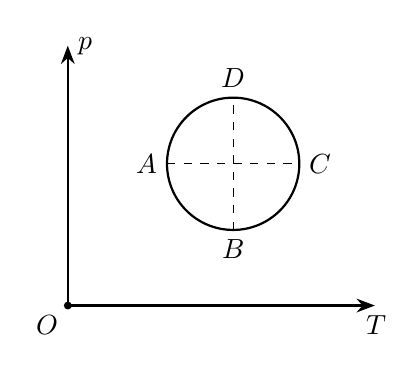
\begin{tikzpicture}[>=Stealth, scale=0.6]
        % 1. Định nghĩa các thông số cơ bản
        \coordinate (O) at (0,0);
        \coordinate (M) at (3.5, 3); % Tâm của đường tròn
        \def\R{1.4}                 % Bán kính đường tròn

        % 2. Vẽ hệ trục tọa độ p-T
        \draw[->, thick] (0,0) -- (6.5,0) node[below, black] {$T$};
        \draw[->, thick] (0,0) -- (0,5.5) node[right, black] {$p$};
        
        % Điểm gốc O (chấm đỏ viền đen)
        \filldraw[draw] (O) circle (2pt) node[below left, black] {$O$};

        % 3. Vẽ đường tròn chính màu đỏ
        \draw[thick] (M) circle (\R);

        % 4. Vẽ các đường nét đứt và nhãn cardinal A, B, C, D
        \coordinate (A) at ($(M)+(-\R,0)$);
        \coordinate (B) at ($(M)+(0,-\R)$);
        \coordinate (C) at ($(M)+(\R,0)$);
        \coordinate (D) at ($(M)+(0,\R)$);
        \draw[dashed] (A) node [left] {$A$} -- (C) node  [right] {$C$};
        \draw[dashed] (B) node [below] {$B$} -- (D) node  [above] {$D$};
    \end{tikzpicture}
}
    \loigiai{
        \begin{itemchoice}
        \itemch Ta có ${\frac{pV}{T} = C \Rightarrow p = \frac{C}{V} \cdot T}$. \\
        Hệ số góc của đường đẳng tích trên đồ thị ${p-T}$ là ${\frac{C}{V}}$. \\
        Hệ số góc càng nhỏ thì ${V}$ càng lớn
        \itemch
        \itemch
        \itemch Quá trình ${D \to A}$, thể tích của khối khí giảm rồi tăng
            \begin{center}
                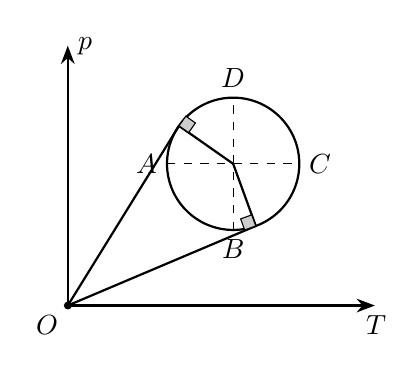
\begin{tikzpicture}[>=Stealth, scale=0.6]
                    % 1. Định nghĩa các thông số cơ bản
                    \coordinate (O) at (0,0);
                    \coordinate (M) at (3.5, 3); % Tâm của đường tròn
                    \def\R{1.4}                 % Bán kính đường tròn

                    % 2. Vẽ hệ trục tọa độ p-T
                    \draw[->, thick] (0,0) -- (6.5,0) node[below, black] {$T$};
                    \draw[->, thick] (0,0) -- (0,5.5) node[right, black] {$p$};
                    
                    % Điểm gốc O (chấm đỏ viền đen)
                    \filldraw[draw] (O) circle (2pt) node[below left, black] {$O$};

                    % 3. Vẽ đường tròn chính màu đỏ
                    \draw[thick] (M) circle (\R);

                    % 4. Vẽ các đường nét đứt và nhãn cardinal A, B, C, D
                    \coordinate (A) at ($(M)+(-\R,0)$);
                    \coordinate (B) at ($(M)+(0,-\R)$);
                    \coordinate (C) at ($(M)+(\R,0)$);
                    \coordinate (D) at ($(M)+(0,\R)$);
                    \draw[dashed] (A) node [left] {$A$} -- (C) node  [right] {$C$};
                    \draw[dashed] (B) node [below] {$B$} -- (D) node  [above] {$D$};

                    % 5. Xác định các tiếp điểm bằng tọa độ cực tương đối
                    % Góc 145 độ cho tiếp điểm trên, 290 độ cho tiếp điểm dưới (ước lượng theo hình)
                    \coordinate (T1) at ($(M)+({\R*cos(145)},{\R*sin(145)})$);
                    \coordinate (T2) at ($(M)+({\R*cos(290)},{\R*sin(290)})$);

                    % 6. Vẽ các đường tiếp tuyến và bán kính
                    \draw[thick] (O) -- (T1);
                    \draw[thick] (O) -- (T2);
                    \draw[thick] (M) -- (T1);
                    \draw[thick] (M) -- (T2);

                    % 7. Vẽ ký hiệu góc vuông tại các tiếp điểm
                    % Góc vuông tại T1
                    \begin{scope}[shift={(T1)}, rotate=145]
                        \draw[fill=gray!40] (0,0) -- (-0.25,0) -- (-0.25,-0.25) -- (0,-0.25) -- cycle;
                    \end{scope}
                    
                    % Góc vuông tại T2
                    \begin{scope}[shift={(T2)}, rotate=290]
                        \draw[fill=gray!40] (0,0) -- (-0.25,0) -- (-0.25,-0.25) -- (0,-0.25) -- cycle;
                    \end{scope}

                \end{tikzpicture}
            \end{center}
        \end{itemchoice}
    }
\end{ex}


% Câu 4
\begin{ex}
\immini[thm]{
    Một học sinh làm thí nghiệm ``Làm đá từ nước muối'':\\
    \textit{Bước 1:} Pha nước muối đặc và đựng trong bình thủy tinh.\\
    \textit{Bước 2:} Cho bình nước muối đặc vào trong tủ lạnh một thời gian đủ dài.\\
    \textit{Bước 3:} Lấy bình nước muối ra khỏi tủ lạnh và đặt một ống nghiệm chứa nước vào trong nước muối, như hình vẽ bên.\\
    \textit{Bước 4:} Quan sát trạng thái (thể) của nước trong ống nghiệm và ghi lại dữ liệu nhiệt độ của nước muối và nước vào bảng bên dưới theo thời gian.\\
    Trong suốt thí nghiệm, nước muối dù ở nhiệt độ thấp vẫn ở trạng thái lỏng.\\
    \begin{center}
    \begin{tabular}{|l|c|c|c|c|c|}
    \hline
    Thời gian ${\tau}$ (phút) & $0$ & $1$ & $2$ & $3$ & $4$ \\
    \hline
    Nhiệt độ nước muối ${t_a}$ (${^\circ\mathrm{C}}$) & $-10$ & $-8$ & $-6$ & $-4$ & $-2$ \\
    \hline
    Nhiệt độ nước ${t_b}$ (${^\circ\mathrm{C}}$) & $10$ & $5$ & $0$ & $0$ & $0$ \\
    \hline
    Trạng thái (thể) của nước & \multicolumn{2}{c|}{Lỏng} & \multicolumn{3}{c|}{Lỏng và rắn} \\
    \hline
    \end{tabular}
    \end{center}
}{
    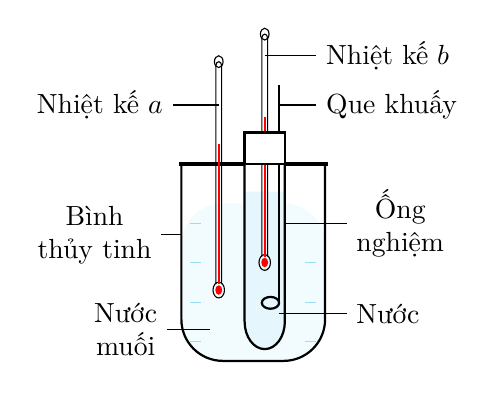
\begin{tikzpicture}[>=Stealth, font=\linespread{1}\selectfont, xscale=0.73, scale=0.5]
        % --- Các tọa độ cơ bản ---
        \coordinate (O) at (0,0);
        
        % --- 1. Vẽ Bình thủy tinh và Nước muối ---
        % Đổ màu nước muối
        \fill[cyan!5, rounded corners=15pt] (-3.5, 4) -- (-3.5, 0) -- (1.5, 0) -- (1.5, 4) -- cycle;
        % Các vạch nước muối (trang trí)
        \foreach \y in {0.5, 1.5, 2.5, 3.5} {
            \draw[cyan!40, very thin] (-3.2, \y) -- (-2.8, \y) (1.2, \y) -- (0.8, \y);
        }
        % Thành bình
        \draw[thick, rounded corners=15pt] (-3.5, 5) -- (-3.5, 0) -- (1.5, 0) -- (1.5, 5);
        % Nắp bình
        \draw[very thick] (-3.6, 5) -- (1.6, 5);

        % --- 2. Vẽ Ống nghiệm và Nước ---
        % Thân ống nghiệm
        \fill[white] (-1.3, 5) -- (-1.3, 1) arc(180:360:0.7) -- (0.1, 5) -- cycle;
        % Nước trong ống nghiệm
        \fill[cyan!20, opacity=0.5] (-1.3, 4.3) -- (-1.3, 1) arc(180:360:0.7) -- (0.1, 4.3) -- cycle;
        \draw[thick] (-1.3, 5.8) -- (-1.3, 1) arc(180:360:0.7) -- (0.1, 5.8);

        % --- 3. Vẽ các Nhiệt kế ---
        % Nhiệt kế a (bên ngoài)
        \draw (-2.2, 1.8) circle (0.2); % Bầu nhiệt kế
        \draw (-2.3, 1.95) -- (-2.3, 7.5) arc(180:0:0.1) -- (-2.1, 1.95);
        \draw (-2.2, 7.6) circle (0.15); % Đầu trên
        \fill[red] (-2.2, 1.8) circle (0.12); % Chất lỏng đỏ
        \fill[red] (-2.23, 1.95) rectangle (-2.17, 5.5);

        % Nhiệt kế b (trong ống nghiệm)
        \draw (-0.6, 2.5) circle (0.2);
        \draw (-0.7, 2.65) -- (-0.7, 8.2) arc(180:0:0.1) -- (-0.5, 2.65);
        \draw (-0.6, 8.3) circle (0.15);
        \fill[red] (-0.6, 2.5) circle (0.12);
        \fill[red] (-0.63, 2.65) rectangle (-0.57, 6.2);

        % --- 4. Vẽ Que khuấy ---
        \draw[thick] (-0.1, 7) -- (-0.1, 1.5);
        \draw[thick] (-0.4, 1.475) ellipse (0.3 and 0.15);

        % --- 5. Chú thích (Labels) ---
        % Nhóm bên trái
        \draw (-2.2, 6.5) -- (-3.8, 6.5) node[left] {Nhiệt kế $a$};
        \draw (-3.5, 3.2) -- (-4.2, 3.2) node[left, align=center] {Bình\\thủy tinh};
        \draw (-2.5, 0.8) -- (-4.0, 0.8) node[left, align=center] {Nước\\muối};

        % Nhóm bên phải
        \draw (-0.6, 7.75) -- (1.2, 7.75) node[right] {Nhiệt kế $b$};
        \draw (-0.1, 6.5) -- (1.2, 6.5) node[right] {Que khuấy};
        \draw (0.1, 3.5) -- (2.25, 3.5) node[right, align=center] {Ống\\nghiệm};
        \draw (-0.1, 1.2) -- (2.25, 1.2) node[right] {Nước};

        % Khối nắp ống nghiệm trên nắp bình
        \draw[fill=white, thick] (-1.3, 5) rectangle (0.1, 5.8);
    \end{tikzpicture}
}
    \choiceTF[1]
    {Nước muối tỏa nhiệt và nước thu nhiệt}
    {Trong phút thứ ba và thứ tư, tổng thế năng phân tử nước (ở thể lỏng và rắn) trong ống nghiệm tăng}
    {Nhiệt độ nóng chảy của nước muối lớn hơn ${-10^\circ\mathrm{C}}$}
    {Học sinh nhận thấy rằng nước muối nóng lên chậm hơn nước nguội đi; và dựa vào điều này, học sinh kết luận: ``Nhiệt dung riêng của nước muối lớn hơn nhiệt dung riêng của nước''}
    \loigiai{
        \begin{itemchoice}
        \itemch Nước muối thu nhiệt (nhiệt độ tăng) và nước tỏa nhiệt (nhiệt độ giảm)
        \itemch Trong phút thứ ba và thứ tư, nước tỏa nhiệt để đông đặc ${\Rightarrow}$ nội năng giảm mà nhiệt độ không đổi ${\Rightarrow}$ động năng phân tử không đổi ${\Rightarrow}$ tổng thế năng phân tử giảm
        \itemch Nhiệt độ ${> -10^\circ\mathrm{C}}$ thì nước muối đã ở trạng thái lỏng như đề cho rồi
        \itemch Chưa biết khối lượng của nước muối và nước nên chưa thể kết luận về nhiệt dung riêng
        \end{itemchoice}
    }
\end{ex}


% Câu 1
\begin{ex}
    Ban đầu có ${N_0}$ hạt nhân của một chất phóng xạ. Giả sử sau ${6}$ giờ, tính từ lúc ban đầu, có ${75\%}$ số hạt nhân ${N_0}$ bị phân rã. Chu kì bán rã của chất đó là bao nhiêu giờ?
    \shortans{3}
    \loigiai{
        Số hạt nhân bị phân rã: ${\Delta N = N_0 \left(1 - 2^{-\frac{t}{T}}\right) \Rightarrow 0{,}75 = 1 - 2^{-\frac{6}{T}} \Rightarrow T = 3 \, \mathrm{h}}$
    }
\end{ex}


% Câu 2
\begin{ex}
    Trong một từ trường đều, một đoạn dây dẫn dài ${0{,}4 \, \mathrm{m}}$ đặt vuông góc với đường sức từ. Nếu dòng điện có cường độ ${5 \, \mathrm{A}}$ chạy qua đoạn dây thì lực từ tác dụng lên đoạn dây có độ lớn là ${0{,}28 \, \mathrm{N}}$. Độ lớn cảm ứng từ của từ trường là bao nhiêu ${\mathrm{T}}$?
    \shortans{0,14}
    \loigiai{
        Lực từ tác dụng lên đoạn dây: ${F = ILB\sin\alpha \Rightarrow 0{,}28 = 5 \cdot 0{,}4 \cdot B \cdot \sin 90^\circ \Rightarrow B = 0{,}14 \, \mathrm{T}}$
    }
\end{ex}


% Câu 3
\begin{ex}
    Một cuộn dây gồm ${200}$ vòng dây đặt trong từ trường. Độ biến thiên từ thông qua một vòng dây trong ${0{,}02 \, \mathrm{s}}$ là ${6 \cdot 10^{-5} \, \mathrm{Wb}}$. Độ lớn suất điện động cảm ứng trong cuộn dây là bao nhiêu ${\mathrm{V}}$?
    \shortans{0,6}
    \loigiai{
        Độ lớn suất điện động cảm ứng: ${e = \left| \frac{N\Delta\phi}{\Delta t} \right| = \frac{200 \cdot 6 \cdot 10^{-5}}{0{,}02} = 0{,}6 \, \mathrm{V}}$
    }
\end{ex}


% Câu 4
\begin{ex}
    Một khối hợp kim có khối lượng ${0{,}5 \, \mathrm{kg}}$ được đưa vào lò nung ở nhiệt độ ${828^\circ\mathrm{C}}$ trong thời gian đủ dài, sau đó nhanh chóng lấy ra cho vào ${5 \, \mathrm{kg}}$ nước ở ${20^\circ\mathrm{C}}$ để làm nguội. Cuối cùng, nhiệt độ của nước là bao nhiêu ${^\circ\mathrm{C}}$? Biết nhiệt dung riêng của nước là ${4200 \, \mathrm{J/(kg \cdot K)}}$ và nhiệt dung riêng của hợp kim là ${420 \, \mathrm{J/(kg \cdot K)}}$.
    \shortans{28}
    \loigiai{
        Phương trình cân bằng nhiệt: ${m_{hk}c_{hk}(t_{hk} - t) = m_nc_n(t - t_n)}$\\
        ${\Rightarrow t = \frac{m_{hk}c_{hk}t_{hk} + m_nc_nt_n}{m_{hk}c_{hk} + m_nc_n} = \frac{0{,}5 \cdot 420 \cdot 828 + 5 \cdot 4200 \cdot 20}{0{,}5 \cdot 420 + 5 \cdot 4200} = 28^\circ\mathrm{C}}$
    }
\end{ex}


% Câu 5
\begin{ex}
    Một bình oxy sử dụng trong phòng thí nghiệm có thể tích ${0{,}18 \, \mathrm{m^3}}$ và áp suất khí oxy bên trong là ${10 \, \mathrm{atm}}$. Phòng thí nghiệm tiêu thụ ${0{,}36 \, \mathrm{m^3}}$ oxy mỗi ngày ở áp suất ${1 \, \mathrm{atm}}$. Khi áp suất trong bình giảm xuống ${2 \, \mathrm{atm}}$, cần phải nạp lại. Coi nhiệt độ của oxy không đổi. Bình có thể cung cấp oxy cho phòng thí nghiệm trong bao nhiêu ngày trước khi cần nạp lại?
    \shortans{4}
    \loigiai{
        Lượng khí ban đầu: ${n = \frac{p V}{RT} = \frac{10 \cdot 0{,}18}{RT}}$.\\
        Lượng khí còn lại trong bình: ${n_1 = \frac{p_1 V}{RT} = \frac{2 \cdot 0{,}18}{RT}}$.\\
        Lượng khí tiêu thụ trong ${t}$ ngày: ${n_2 = \frac{p_2 V_2 \cdot t}{RT} = \frac{1 \cdot 0{,}36 \cdot t}{RT}}$.\\
        Ta có: ${n = n_1 + n_2 \Rightarrow 10 \cdot 0{,}18 = 2 \cdot 0{,}18 + 1 \cdot 0{,}36 \cdot t \Rightarrow t = 4}$ ngày
    }
\end{ex}


% Câu 6
\begin{ex}
    Ban đầu, hai mẫu chất phóng xạ ${A}$ và ${B}$ nguyên chất có khối lượng lần lượt ${m_A}$ và ${m_B}$. Sau đó ${20}$ ngày, khối lượng chất phóng xạ ${A}$ và ${B}$ trong hai mẫu bằng nhau. Biết chu kì bán rã của chất phóng xạ ${A}$ và ${B}$ lần lượt là ${4}$ ngày và ${5}$ ngày. Tỉ số ${\frac{m_A}{m_B}}$ bằng bao nhiêu?
    \shortans{2}
    \loigiai{
        Khối lượng còn lại sau thời gian ${t}$: ${m = m_0 \cdot 2^{-\frac{t}{T}}}$.\\
        Theo đề bài: ${m_A \cdot 2^{-\frac{t}{T_A}} = m_B \cdot 2^{-\frac{t}{T_B}} \Rightarrow \frac{m_A}{m_B} = \frac{2^{-\frac{t}{T_B}}}{2^{-\frac{t}{T_A}}} = \frac{2^{-\frac{20}{5}}}{2^{-\frac{20}{4}}} = \frac{2^{-4}}{2^{-5}} = 2}$
    }
\end{ex}

% Câu 1
\begin{ex}
    Các hạt trong tia phóng xạ nào sau đây không mang điện tích?
    \choice
    {\True Tia $\gamma$}
    {Tia $\beta^+$}
    {Tia $\alpha$}
    {Tia $\beta^-$}
    \loigiai{
        Tia $\gamma$ là sóng điện từ có bước sóng rất ngắn, không mang điện tích.
    }
\end{ex}


% Câu 2
\begin{ex}
    Cho ${4}$ tia phóng xạ: tia $\alpha$, tia $\beta^+$, tia $\beta^-$ và tia $\gamma$ đi vào một miền có điện trường đều theo phương vuông góc với đường sức điện. Tia phóng xạ không bị lệch khỏi phương truyền ban đầu là
    \choice
    {\True tia $\gamma$}
    {tia $\beta^-$}
    {tia $\beta^+$}
    {tia $\alpha$}
    \loigiai{
        Tia phóng xạ $\gamma$ không mang điện $\Rightarrow$ không bị lệch khỏi phương truyền ban đầu.
    }
\end{ex}


% Câu 3
\begin{ex}
    Phát biểu nào sau đây là sai khi nói về hiện tượng phóng xạ?
    \choice
    {Trong phóng xạ $\alpha$, hạt nhân con có số neutron nhỏ hơn số neutron của hạt nhân mẹ}
    {Trong phóng xạ $\beta^-$, hạt nhân mẹ và hạt nhân con có số khối bằng nhau, số proton khác nhau}
    {\True Trong phóng xạ $\beta$, có sự bảo toàn điện tích nên số proton được bảo toàn}
    {Trong phóng xạ $\beta^+$, hạt nhân mẹ và hạt nhân con có số khối bằng nhau, số neutron khác nhau}
    \loigiai{
        Trong phóng xạ $\beta$, số proton không bảo toàn.
    }
\end{ex}


% Câu 4
\begin{ex}
    Phóng xạ và phản ứng hạch hạt nhân
    \choice
    {đều có sự hấp thụ neutron chậm}
    {đều là phản ứng hạt nhân thu năng lượng}
    {đều không phải là phản ứng hạt nhân}
    {\True đều là phản ứng hạt nhân tỏa năng lượng}
    \loigiai{
        Phóng xạ và phản ứng hạch hạt nhân đều là phản ứng hạt nhân tỏa năng lượng.
    }
\end{ex}


% Câu 5
\begin{ex}
    Gọi $c$ là tốc độ ánh sáng trong chân không. Theo thuyết tương đối, một vật có khối lượng nghỉ $m_0$ và khi chuyển động có khối lượng động (khối lượng tương đối tính) là $m$ thì nó có động năng là
    \choice
    {$W_d = (m + m_0)c$}
    {$W_d = (m + m_0)c^2$}
    {\True $W_d = (m - m_0)c^2$}
    {$W_d = (m - m_0)c$}
    \loigiai{
        Động năng của vật theo thuyết tương đối là $W_d = (m - m_0)c^2$.
    }
\end{ex}


% Câu 6
\begin{ex}
    Phát biểu nào sau đây là sai khi nói về phản ứng nhiệt hạch (phản ứng tổng hợp hạt nhân)?
    \choice
    {Sự nổ của bom H (bom khinh khí) là một phản ứng nhiệt hạch không kiểm soát được}
    {\True Sự nổ của bom H (bom khinh khí) là một phản ứng nhiệt hạch kiểm soát được}
    {Phản ứng nhiệt hạch là quá trình kết hợp hai hay nhiều hạt nhân nhẹ thành một hạt nhân nặng hơn}
    {Phản ứng nhiệt hạch là loại phản ứng hạt nhân tỏa năng lượng}
    \loigiai{
        Sự nổ của bom H là phản ứng nhiệt hạch không kiểm soát được.
    }
\end{ex}


% Câu 7
\begin{ex}
    Một trong những lí do các nhà máy điện hạt nhân thường được xây dựng cạnh hồ, sông và bờ biển là vì: nhà máy điện hạt nhân
    \choice
    {thường xuyên nạp nhiên liệu nên cần nhiều nước}
    {thường có công suất phát điện rất lớn}
    {tiêu thụ nhiều nhiên liệu}
    {\True tỏa ra rất nhiều nhiệt, cần nhiều nước để làm mát}
    \loigiai{
        Các nhà máy điện hạt nhân tỏa ra rất nhiều nhiệt, cần nhiều nước để làm mát.
    }
\end{ex}


% Câu 8
\begin{ex}
    Hạt nhân $^{234}_{91}\mathrm{Pa}$ phóng xạ $\beta^-$ và biến đổi thành hạt nhân $\mathrm{X}$. Hạt nhân $\mathrm{X}$ tiếp tục phóng xạ $\alpha$ và biến đổi thành hạt nhân
    \choice
    {$^{234}_{92}\mathrm{U}$}
    {$^{235}_{92}\mathrm{U}$}
    {$^{234}_{90}\mathrm{Th}$}
    {\True $^{230}_{90}\mathrm{Th}$}
    \loigiai{
        $^{234}_{91}\mathrm{Pa} \to \, ^0_{-1}e + \, ^{234}_{92}\mathrm{X}$ \\
        $^{234}_{92}\mathrm{X} \to \, ^4_2\alpha + \, ^{230}_{90}\mathrm{Th}$.
    }
\end{ex}


% Câu 9
\begin{ex}
    \immini[thm]{
        Như hình vẽ, khi hạt alpha bị tán xạ bởi một hạt nhân vàng (chấm đen trên hình), quỹ đạo thể hiện trên hình không thể tồn tại là
        \choice
        {${1}$ và ${4}$}
        {${1}$ và ${2}$}
        {\True ${2}$ và ${3}$}
        {${3}$ và ${4}$}
    }{
        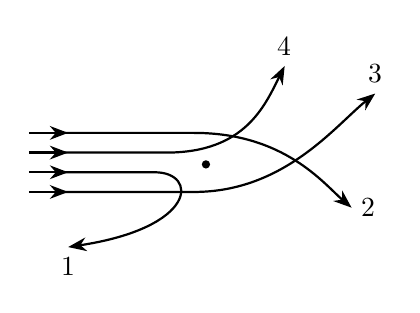
\begin{tikzpicture}[>=Stealth, scale=0.5, thick]
            % Hạt nhân (điểm trung tâm)
            \fill[black] (4.5, 0) circle (3pt);
            % Quỹ đạo 1: Bắt đầu dưới cùng, quay ngược lại (u-turn)
            \draw[->] (0, -0.2) -- (1, -0.2);
            \draw[->] (0.8, -0.2) -- (3.2, -0.2) .. controls (4.3, -0.2) and (4.3, -1.6) .. (1, -2.1) node[below] {$1$};

            % Quỹ đạo 2: Bắt đầu ở giữa trên, lệch xuống dưới
            \draw[->] (0, 0.8) -- (1, 0.8);
            \draw[->] (0.8, 0.8) -- (4.2, 0.8) .. controls (6.5, 0.8) and (7.5, -0.5) .. (8.2, -1.1) node[right] {$2$};

            % Quỹ đạo 3: Bắt đầu ở giữa dưới, lệch lên trên
            \draw[->] (0, -0.7) -- (1, -0.7);
            \draw[->] (0.8, -0.7) -- (4.2, -0.7) .. controls (6.5, -0.7) and (7.8, 1) .. (8.8, 1.8) node[above] {$3$};

            % Quỹ đạo 4: Bắt đầu từ trên cùng, lệch lên trên
            \draw[->] (0, 0.3) -- (1, 0.3);
            \draw[->] (0.8, 0.3) -- (3.5, 0.3) .. controls (5.5, 0.3) and (6, 1.5) .. (6.5, 2.5) node[above] {$4$};
        \end{tikzpicture}
    }
    \loigiai{
        Hạt alpha và hạt nhân đẩy nhau. Quỹ đạo ${2}$ và ${3}$ thể hiện sự hút nhau nên không thể tồn tại.
    }
\end{ex}


% Câu 10
\begin{ex}
    Cho phản ứng hạt nhân: $^{210}_{84}\mathrm{Po} \to \mathrm{X} + \, ^{206}_{82}\mathrm{Pb}$. Hạt $\mathrm{X}$ là
    \choice
    {$^1_1\mathrm{H}$}
    {$^3_2\mathrm{He}$}
    {\True $^4_2\mathrm{He}$}
    {$^3_1\mathrm{H}$}
    \loigiai{
        ${\left\{\begin{aligned} & 210 = A + 206 \\ & 84 = Z + 82 \end{aligned}\right. \Rightarrow \left\{\begin{aligned} & A = 4 \\ & Z = 2 \end{aligned}\right.}$.
    }
\end{ex}


% Câu 11
\begin{ex}
    Polonium $^{210}_{84}\mathrm{Po}$ phóng xạ $\alpha$ và biến đổi thành chì $\mathrm{Pb}$. Biết khối lượng các hạt nhân $\mathrm{Po}$; $\alpha$; $\mathrm{Pb}$ lần lượt là: ${209{,}937303} \, \mathrm{amu}$; ${4{,}001506} \, \mathrm{amu}$; ${205{,}929442} \, \mathrm{amu}$. Năng lượng tỏa ra khi một hạt nhân polonium phân rã xấp xỉ bằng
    \choice
    {\True ${5{,}92} \, \mathrm{MeV}$}
    {${2{,}96} \, \mathrm{MeV}$}
    {${29{,}60} \, \mathrm{MeV}$}
    {${59{,}20} \, \mathrm{MeV}$}
    \loigiai{
        $\Delta E = (m_t - m_s)c^2 = (209{,}937303 - 4{,}001506 - 205{,}929442) \cdot 931{,}5 \approx {5{,}92} \, \mathrm{MeV}$.
    }
\end{ex}


% Câu 12
\begin{ex}
    Cho phản ứng hạt nhân: $^{234}_{92}\mathrm{U} \to \, ^4_2\mathrm{He} + \, ^{230}_{90}\mathrm{Th}$. Gọi $a, b$ và $c$ lần lượt là năng lượng liên kết riêng của hạt nhân uranium, hạt $\alpha$ và hạt nhân thorium. Năng lượng tỏa ra trong phản ứng này bằng
    \choice
    {\True $4b + 230c - 234a$}
    {$230c - 4b - 234a$}
    {$234a - 4b - 230c$}
    {$4b + 230c + 234a$}
    \loigiai{
        $\Delta E = W_{lk\mathrm{He}} + W_{lk\mathrm{Th}} - W_{lk\mathrm{U}} = 4b + 230c - 234a$.
    }
\end{ex}


% Câu 13
\begin{ex}
    Cho phản ứng hạt nhân: $^{12}_{6}{C} + \gamma \to 3 \, ^4_2\mathrm{He}$. Biết khối lượng của $^{12}_{6}{C}$ và $^4_2\mathrm{He}$ lần lượt là ${11{,}9970} \, \mathrm{amu}$ và ${4{,}0015} \, \mathrm{amu}$. Năng lượng nhỏ nhất của photon ứng với bức xạ $\gamma$ để phản ứng xảy ra có giá trị gần nhất với giá trị nào sau đây?
    \choice
    {${6} \, \mathrm{MeV}$}
    {\True ${7} \, \mathrm{MeV}$}
    {${8} \, \mathrm{MeV}$}
    {${9} \, \mathrm{MeV}$}
    \loigiai{
        $E_{\gamma} = (3m_{\mathrm{He}} - m_{{C}})c^2 = (3 \cdot 4{,}0015 - 11{,}997) \cdot 931{,}5 \approx {7} \, \mathrm{MeV}$.
    }
\end{ex}


% Câu 14
\begin{ex}
    Bắn hạt $\alpha$ vào hạt nhân $^{27}_{13}\mathrm{Al}$ đứng yên tạo ra neutron và hạt $\mathrm{X}$. Biết khối lượng các hạt ${m_{\alpha} = {4{,}0016} \, \mathrm{amu}}$; $m_{\mathrm{n}} = {1{,}00866} \, \mathrm{amu}$; $m_{\mathrm{Al}} = {26{,}9744} \, \mathrm{amu}$; $m_{\mathrm{X}} = {29{,}9701} \, \mathrm{amu}$. Hạt neutron và $\mathrm{X}$ có động năng lần lượt là ${4} \, \mathrm{MeV}$ và ${1{,}8} \, \mathrm{MeV}$. Động năng của hạt $\alpha$ là
    \choice
    {${3{,}23} \, \mathrm{MeV}$}
    {${5{,}8} \, \mathrm{MeV}$}
    {${7{,}8} \, \mathrm{MeV}$}
    {\True ${8{,}37} \, \mathrm{MeV}$}
    \loigiai{
        $\Delta E = (m_{\alpha} + m_{\mathrm{Al}} - m_{\mathrm{n}} - m_{\mathrm{X}})c^2 = (4{,}0016 + 26{,}9744 - 1{,}00866 - 29{,}9701) \cdot 931{,}5 = -{2{,}57094} \, \mathrm{MeV}$ \\
        $\Delta E = K_{\mathrm{n}} + K_{\mathrm{X}} - K_{\alpha} \Rightarrow -2{,}57094 = 4 + 1{,}8 - K_{\alpha} \Rightarrow K_{\alpha} \approx {8{,}37} \, \mathrm{MeV}$.
    }
\end{ex}


% Câu 15
\begin{ex}
    Dùng hạt proton có động năng là ${4{,}8} \, \mathrm{MeV}$ bắn vào hạt nhân $^{23}_{11}\mathrm{Na}$ đứng yên tạo ra hạt $\alpha$ và hạt $\mathrm{X}$. Biết động năng của hạt $\alpha$ là ${3{,}2} \, \mathrm{MeV}$ và tốc độ hạt $\alpha$ bằng ${2}$ lần tốc độ hạt $\mathrm{X}$. Năng lượng tỏa ra của phản ứng là
    \choice
    {${1{,}5} \, \mathrm{MeV}$}
    {${3{,}6} \, \mathrm{MeV}$}
    {${1{,}2} \, \mathrm{MeV}$}
    {\True ${2{,}4} \, \mathrm{MeV}$}
    \loigiai{
        $^1_1p + \, ^{23}_{11}\mathrm{Na} \to \, ^4_2\alpha + \, ^{20}_{10}\mathrm{X}$ \\
        $\frac{K_{\alpha}}{K_{\mathrm{X}}} = \frac{\dfrac{1}{2}m_{\alpha}v_{\alpha}^2}{\dfrac{1}{2}m_{\mathrm{X}}v_{\mathrm{X}}^2} = \frac{3{,}2}{K_{\mathrm{X}}} = \frac{4}{20} \cdot 2^2 \Rightarrow K_{\mathrm{X}} = {4} \, \mathrm{MeV}$ \\
        $\Delta E = K_{\alpha} + K_{\mathrm{X}} - K_p = 3{,}2 + 4 - 4{,}8 = {2{,}4} \, \mathrm{MeV}$.
    }
\end{ex}


% Câu 16
\begin{ex}
    Dùng hạt proton có động năng ${1{,}6} \, \mathrm{MeV}$ bắn vào hạt nhân liti ($^7_3\mathrm{Li}$) đứng yên. Giả sử sau phản ứng thu được hai hạt giống nhau có cùng động năng và không kèm theo tia $\gamma$. Biết năng lượng tỏa ra của phản ứng là ${17{,}4} \, \mathrm{MeV}$. Động năng của mỗi hạt sinh ra là
    \choice
    {${19{,}0} \, \mathrm{MeV}$}
    {${15{,}8} \, \mathrm{MeV}$}
    {\True ${9{,}5} \, \mathrm{MeV}$}
    {${7{,}9} \, \mathrm{MeV}$}
    \loigiai{
        $\Delta E = 2K_{\mathrm{X}} - K_p \Rightarrow 17{,}4 = 2K_{\mathrm{X}} - 1{,}6 \Rightarrow K_{\mathrm{X}} = {9{,}5} \, \mathrm{MeV}$.
    }
\end{ex}


% Câu 17
\begin{ex}
    Dùng hạt proton có động năng ${5{,}45} \, \mathrm{MeV}$ bắn vào hạt nhân $^9_4\mathrm{Be}$ đứng yên gây ra phản ứng sau: ${{}^1_1p + \, ^9_4\mathrm{Be} \to \mathrm{X} + \alpha + {2{,}15} \, \mathrm{MeV}}$. Tỉ số giữa tốc độ hạt $\alpha$ và hạt $\mathrm{X}$ sau phản ứng là $\frac{4}{3}$. Động năng hạt $\alpha$ là
    \choice
    {${1{,}790} \, \mathrm{MeV}$}
    {${4{,}343} \, \mathrm{MeV}$}
    {\True ${4{,}122} \, \mathrm{MeV}$}
    {${3{,}575} \, \mathrm{MeV}$}
    \loigiai{
        $^1_1p + \, ^9_4\mathrm{Be} \to \, ^6_3\mathrm{X} + \, ^4_2\alpha$ \\
        $\frac{K_{\alpha}}{K_{\mathrm{X}}} = \frac{\dfrac{1}{2}m_{\alpha}v_{\alpha}^2}{\dfrac{1}{2}m_{\mathrm{X}}v_{\mathrm{X}}^2} = \frac{4}{6} \cdot \left(\frac{4}{3}\right)^2 = \frac{32}{27}$ (1) \\
        $\Delta E = K_{\alpha} + K_{\mathrm{X}} - K_p \Rightarrow 2{,}15 = K_{\alpha} + K_{\mathrm{X}} - 5{,}45 \Rightarrow K_{\alpha} + K_{\mathrm{X}} = {7{,}6}$ (2) \\
        Từ (1) và (2) $\Rightarrow K_{\alpha} \approx {4{,}122} \, \mathrm{MeV}$.
    }
\end{ex}


% Câu 18
\begin{ex}
    Dùng hạt $\alpha$ có động năng ${4{,}01} \, \mathrm{MeV}$ bắn vào hạt nhân $^{14}_7\mathrm{N}$ đứng yên thì thu được một hạt proton và một hạt nhân $\mathrm{X}$. Phản ứng này thu năng lượng ${1{,}21} \, \mathrm{MeV}$ và không kèm theo bức xạ gamma. Biết tỉ số giữa tốc độ của hạt proton và tốc độ của hạt $\mathrm{X}$ bằng ${8{,}5}$. Lấy khối lượng các hạt nhân tính theo đơn vị $\mathrm{amu}$ bằng số khối của chúng. Tốc độ của hạt $\mathrm{X}$ là
    \choice
    {${9{,}73 \cdot 10^6} \, \mathrm{m/s}$}
    {${3{,}63 \cdot 10^6} \, \mathrm{m/s}$}
    {\True ${2{,}46 \cdot 10^6} \, \mathrm{m/s}$}
    {${3{,}36 \cdot 10^6} \, \mathrm{m/s}$}
    \loigiai{
        $^4_2\alpha + \, ^{14}_7\mathrm{N} \to \, ^1_1p + \, ^{17}_8\mathrm{X}$ \\
        $\frac{K_p}{K_{\mathrm{X}}} = \frac{\dfrac{1}{2}m_pv_p^2}{\dfrac{1}{2}m_{\mathrm{X}}v_{\mathrm{X}}^2} = \frac{1}{17} \cdot 8{,}5^2 = {4{,}25}$ (1) \\
        $\Delta E = K_p + K_{\mathrm{X}} - K_{\alpha} \Rightarrow -1{,}21 = K_p + K_{\mathrm{X}} - 4{,}01 \Rightarrow K_p + K_{\mathrm{X}} = {2{,}8} \, \mathrm{MeV}$ (2) \\
        Từ (1) và (2) $\Rightarrow K_{\mathrm{X}} = \frac{8}{15} \, \mathrm{MeV}$ \\
        $K_{\mathrm{X}} = \frac{1}{2}m_{\mathrm{X}}v_{\mathrm{X}}^2 \Rightarrow \frac{8}{15} \cdot 1{,}6 \cdot 10^{-13} = \frac{1}{2} \cdot 17 \cdot 1{,}6605 \cdot 10^{-27} \cdot v_{\mathrm{X}}^2 \Rightarrow v_{\mathrm{X}} \approx {2{,}46 \cdot 10^6} \, \mathrm{m/s}$.
    }
\end{ex}


% Câu 1
\begin{ex}
    Cho các kết luận bên dưới về phản ứng hạt nhân: $^3_2\mathrm{He} + \, ^2_1\mathrm{H} \to \, ^4_2\mathrm{He} + \mathrm{Y}$.
    \choiceTF[1]
    {Phản ứng này là phóng xạ $\alpha$}
    {\True $\mathrm{Y}$ là proton}
    {Tổng khối lượng của các hạt sản phẩm lớn hơn tổng khối lượng của các hạt tham gia}
    {\True Tổng năng lượng liên kết của các hạt sản phẩm lớn hơn tổng năng lượng liên kết của các hạt tham gia}
    \loigiai{
        \begin{itemchoice}
        \itemch Phản ứng nhiệt hạch
        \itemch $^3_2\mathrm{He} + \, ^2_1\mathrm{H} \to \, ^4_2\mathrm{He} + \, ^1_1p$
        \itemch $\Delta E = (m_t - m_s)c^2 > 0 \Rightarrow m_t > m_s$
        \itemch $\Delta E = W_{lks} - W_{lkt} > 0 \Rightarrow W_{lks} > W_{lkt}$
        \end{itemchoice}
    }
\end{ex}


% Câu 2
\begin{ex}
    \immini[thm]{
        Hạt phóng xạ ${A}$ thực hiện chuỗi phóng xạ ${A} \to {B} \to {C} \to {D}$ để tạo thành hạt nhân ${D}$. Biết số proton (${p}$) và số neutron (${n}$) trong các hạt nhân ${A, B, C, D}$ biến đổi như đồ thị hình vẽ.
        \choiceTF[1]
        {\True Phóng xạ ${A} \to {B}$ là phóng xạ $\alpha$}
        {Phóng xạ ${B} \to {C}$ là phóng xạ $\beta^+$}
        {\True $x - y = 2$}
        {\True Hạt nhân ${A}$ và hạt nhân ${D}$ là đồng vị của nhau}
    }{
        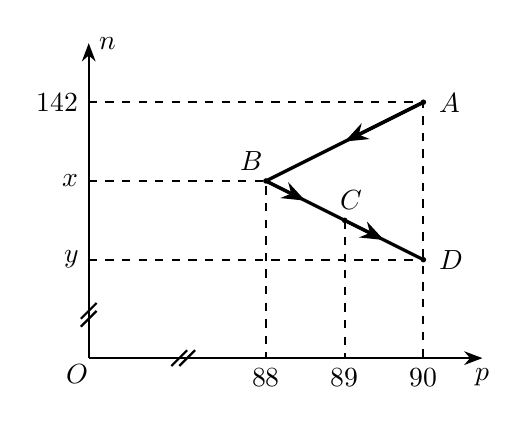
\begin{tikzpicture}[>=Stealth, thick, scale=0.5]
            % --- Các trục tọa độ ---
            \draw[thick, ->] (0,0) -- (10,0) node[below] {$p$};
            \draw[thick, ->] (0,0) -- (0,8) node[right] {$n$};
            \node at (-0.3,-0.4) {$O$};

            % --- Ký hiệu ngắt trục (Break marks) ---
            % Trục N
            \draw[thick] (-0.2, 0.8) -- (0.2, 1.2);
            \draw[thick] (-0.2, 1.0) -- (0.2, 1.4);
            % Trục P
            \draw[thick] (2.1, -0.2) -- (2.5, 0.2);
            \draw[thick] (2.3, -0.2) -- (2.7, 0.2);

            % --- Tọa độ các điểm chính (quy đổi tỉ lệ) ---
            % P: 88 -> 4.5, 89 -> 6.5, 90 -> 8.5
            % N: y -> 2.5, x -> 4.5, 142 -> 6.5
            \coordinate (A) at (8.5, 6.5);
            \coordinate (B) at (4.5, 4.5);
            \coordinate (C) at (6.5, 3.5);
            \coordinate (D) at (8.5, 2.5);

            % --- Các đường dóng (Dashed lines) ---
            \draw[dashed] (0, 6.5) node[left] {$142$} -- (A) -- (8.5, 0) node[below] {$90$};
            \draw[dashed] (0, 4.5) node[left] {$x$} -- (B) -- (4.5, 0) node[below] {$88$};
            \draw[dashed] (0, 2.5) node[left] {$y$} -- (D);
            \draw[dashed] (C) -- (6.5, 0) node[below] {$89$};

            % --- Đồ thị và mũi tên hướng ---
            % Đoạn A-B
            \draw[very thick] (A) -- (B);
            \draw[very thick, ->] (A) -- (6.5, 5.5); % Mũi tên giữa đoạn
            
            % Đoạn B-C-D
            \draw[very thick] (B) -- (D);
            \draw[very thick, ->] (B) -- (5.5, 4.0); % Mũi tên giữa B-C
            \draw[very thick, ->] (C) -- (7.5, 3.0); % Mũi tên giữa C-D

            % --- Vẽ các điểm và nhãn ---
            \foreach \p/\pos in {A/right, B/above left, C/above, D/right} {
                \fill (\p) circle (2pt);
                \node[\pos, xshift=2pt] at (\p) {$\p$};
            }

        \end{tikzpicture}
    }
    \loigiai{
        \begin{itemchoice}
        \itemch $^{90+142}_{90}{A} \to \, ^{88+140}_{88}{B} + \, ^4_2\alpha \Rightarrow x = 140$
        \itemch $^{88+140}_{88}{B} \to \, ^{89+139}_{89}{C} + \, ^0_{-1}e$ là phóng xạ $\beta^-$
        \itemch $^{89+139}_{89}{C} \to \, ^{90+138}_{90}{D} + \, ^0_{-1}e \Rightarrow y = 138 \to x - y = 2$
        \itemch ${A}$ và ${D}$ có cùng $Z = 90$ và khác số neutron
        \end{itemchoice}
    }
\end{ex}


% Câu 3
\begin{ex}
    Một lò phản ứng hạt nhân của nhà máy điện hạt nhân sử dụng nhiên liệu uranium. Một trong những phản ứng hạt nhân xảy ra trong lò là: $\mathrm{X} + \, ^{235}_{92}\mathrm{U} \to \, ^{139}_{54}\mathrm{Xe} + \, ^{95}_{38}\mathrm{Sr} + 2\mathrm{X}$. Biết năng lượng liên kết riêng của hạt nhân $^{235}_{92}\mathrm{U}$, $^{139}_{54}\mathrm{Xe}$, $^{95}_{38}\mathrm{Sr}$ lần lượt là ${7{,}6} \, \mathrm{MeV/nucleon}$; ${8{,}4} \, \mathrm{MeV/nucleon}$; ${8{,}7} \, \mathrm{MeV/nucleon}$.
    \choiceTF[1]
    {Phản ứng trên là phản ứng tổng hợp hạt nhân}
    {Hạt $\mathrm{X}$ trong phản ứng trên là proton}
    {Sau khi đưa vào lò phản ứng hạt nhân, chu kì bán rã của uranium $^{235}_{92}\mathrm{U}$ trở nên ngắn hơn}
    {\True Nếu dùng hết ${1} \, \mathrm{kg}$ uranium $^{235}_{92}\mathrm{U}$ theo phản ứng trên thì sẽ tỏa ra năng lượng là ${8{,}5 \cdot 10^{13}} \, \mathrm{J}$}
    \loigiai{
        \begin{itemchoice}
        \itemch Phản ứng trên là phản ứng phân hạch
        \itemch Hạt $\mathrm{X}$ trong phản ứng trên là neutron
        \itemch Chu kì bán rã của uranium $^{235}_{92}\mathrm{U}$ không đổi
        \itemch $\Delta E = W_{lk\mathrm{Xe}} + W_{lk\mathrm{Sr}} - W_{lk\mathrm{U}} = 139 \cdot 8{,}4 + 95 \cdot 8{,}7 - 235 \cdot 7{,}6 = {208{,}1} \, \mathrm{MeV}$ \\
        $n = \frac{m}{M} = \frac{10^3}{235} = \frac{200}{47} \, \mathrm{mol}$ \\
        $N = nN_A = \frac{200}{47} \cdot 6{,}02 \cdot 10^{23} \approx {2{,}56 \cdot 10^{24}}$ \\
        $Q = N\Delta E = 2{,}56 \cdot 10^{24} \cdot 208{,}1 \cdot 1{,}6 \cdot 10^{-13} \approx {8{,}5 \cdot 10^{13}} \, \mathrm{J}$
        \end{itemchoice}
    }
\end{ex}


% Câu 4
\begin{ex}
    Một nhà máy điện hạt nhân dùng nhiên liệu uranium $^{235}_{92}\mathrm{U}$ có công suất phát điện ${550} \, \mathrm{MW}$ và hiệu suất chuyển hóa năng lượng hạt nhân thành điện năng là ${20}\%$. Biết một hạt nhân uranium $^{235}_{92}\mathrm{U}$ phân hạch thì tỏa ra năng lượng là ${3{,}2 \cdot 10^{-11}} \, \mathrm{J}$ và biết khối lượng mol của $^{235}_{92}\mathrm{U}$ là ${235} \, \mathrm{g/mol}$.
    \choiceTF[1]
    {\True Các nhà máy điện hạt nhân hiện nay đều sử dụng phản ứng phân hạch hạt nhân}
    {\True Sau mỗi phản ứng, trung bình có một neutron trong số các neutron sinh ra gây phản ứng tiếp theo}
    {Năng lượng điện nhà máy cung cấp trong ${1}$ giờ là ${1{,}89 \cdot 10^{12}} \, \mathrm{J}$}
    {Nếu hoạt động liên tục thì lượng uranium $^{235}_{92}\mathrm{U}$ mà nhà máy cần dùng trong ${365}$ ngày là ${962} \, \mathrm{kg}$}
    \loigiai{
        \begin{itemchoice}
        \itemch 
        \itemch 
        \itemch $A = Pt = 550 \cdot 10^6 \cdot 60 \cdot 60 = {1{,}98 \cdot 10^{12}} \, \mathrm{J}$
        \itemch $A' = Pt' = 550 \cdot 10^6 \cdot 365 \cdot 24 \cdot 60 \cdot 60 = {1{,}73448 \cdot 10^{16}}$ \\
        $Q = \frac{A'}{H} = \frac{1{,}73448 \cdot 10^{16}}{0{,}2} = {8{,}6724 \cdot 10^{16}} \, \mathrm{J}$ \\
        $N = \frac{Q}{\Delta E} = \frac{8{,}6724 \cdot 10^{16}}{3{,}2 \cdot 10^{-11}} = {2{,}710125 \cdot 10^{23}}$ \\
        $n = \frac{N}{N_A} = \frac{2{,}710125 \cdot 10^{23}}{6{,}02 \cdot 10^{23}} \approx {4{,}5 \cdot 10^3} \, \mathrm{mol}$ \\
        $m = nM = 4{,}5 \cdot 10^3 \cdot 0{,}235 > {962} \, \mathrm{kg}$
        \end{itemchoice}
    }
\end{ex}


% Câu 1
\begin{ex}
    Hạt nhân $^{60}\mathrm{Ni}$ có điện tích là $+28e$. Có bao nhiêu neutron trong hạt nhân $^{58}\mathrm{Ni}$?
    \shortans{30}
    \loigiai{
        $N = A - Z = 58 - 28 = 30$.
    }
\end{ex}


% Câu 2
\begin{ex}
    Lò phản ứng hạt nhân Đà Lạt có công suất ${500{,}0} \, \mathrm{kW}$ và sử dụng nhiên liệu là $^{235}_{92}\mathrm{U}$. Coi mỗi hạt nhân $^{235}_{92}\mathrm{U}$ phân hạch tỏa ra năng lượng trung bình là ${175} \, \mathrm{MeV}$ và uranium chỉ bị tiêu hao bởi quá trình phân hạch. Khối lượng mol của $\mathrm{U235}$ lấy bằng ${235} \, \mathrm{g/mol}$. Khối lượng $^{235}_{92}\mathrm{U}$ mà lò tiêu thụ nếu hoạt động liên tục trong ${72}$ giờ là bao nhiêu $\mathrm{g}$ (làm tròn kết quả đến chữ số hàng phần mười)?
    \shortans{1,8}
    \loigiai{
        $A = Pt = 500 \cdot 10^3 \cdot 72 \cdot 60 \cdot 60 = {1{,}296 \cdot 10^{11}} \, \mathrm{J}$ \\
        $N = \frac{A}{\Delta E} = \frac{1{,}296 \cdot 10^{11}}{175 \cdot 1{,}6 \cdot 10^{-13}} \approx {4{,}63 \cdot 10^{21}}$ \\
        $n = \frac{N}{N_A} = \frac{4{,}63 \cdot 10^{21}}{6{,}02 \cdot 10^{23}} \approx {7{,}7 \cdot 10^{-3}} \, \mathrm{mol}$ \\
        $m = nM = 7{,}7 \cdot 10^{-3} \cdot 235 \approx {1{,}8} \, \mathrm{g}$.
    }
\end{ex}


% Câu 3
\begin{ex}
    \sochc{2}{Trong một mẫu quặng uranium, người ta thấy có lẫn chì $^{206}_{82}\mathrm{Pb}$ cùng với $^{238}_{92}\mathrm{U}$. Biết rằng toàn bộ chì được tạo ra có nguồn gốc từ uranium $^{238}\mathrm{U}$ và không hề bị thất thoát vào môi trường. Cho chu kì bán rã của $^{238}_{92}\mathrm{U}$ là ${4{,}47}$ tỉ năm.}
    \begin{chc}
        Nếu cứ ${1}$ nguyên tử $^{206}_{82}\mathrm{Pb}$ thì có ${5}$ nguyên tử $^{238}_{92}\mathrm{U}$ thì tuổi của mẫu quặng là bao nhiêu tỉ năm (làm tròn kết quả đến chữ số hàng phần trăm)?
        \shortans{1,18}
        \loigiai{
            $\frac{\Delta N}{N} = \frac{N_0 \left(1 - 2^{-\frac{t}{T}}\right)}{N_0 \cdot 2^{-\frac{t}{T}}} = \frac{1}{5} \Rightarrow 2^{\frac{t}{T}} - 1 = \frac{1}{5} \Rightarrow 2^{\frac{t}{4{,}47}} = \frac{6}{5} \Rightarrow t \approx {1{,}18}$ tỉ năm.
        }
    \end{chc}
    \begin{chc}
        Khối lượng mol tính theo gam xem bằng số khối của hạt nhân của nó. Nếu cứ ${1} \, \mathrm{g}$ $^{206}_{82}\mathrm{Pb}$ thì có ${5} \, \mathrm{g}$ $^{238}_{92}\mathrm{U}$ thì tuổi của mẫu quặng là bao nhiêu tỉ năm (làm tròn kết quả đến chữ số hàng phần trăm)?
        \shortans{1,34}
        \loigiai{
            $\frac{m_{\mathrm{Pb}}}{m_{\mathrm{U}}} = \frac{\Delta N}{N} \cdot \frac{A_{\mathrm{Pb}}}{A_{\mathrm{U}}} \Rightarrow \frac{1}{5} = \frac{\Delta N}{N} \cdot \frac{206}{238} \Rightarrow \frac{\Delta N}{N} = \frac{119}{515}$ \\
            $\frac{\Delta N}{N} = \frac{N_0 \left(1 - 2^{-\frac{t}{T}}\right)}{N_0 \cdot 2^{-\frac{t}{T}}} = 2^{\frac{t}{T}} - 1 \Rightarrow 2^{\frac{t}{T}} = 1 + \frac{119}{515} = \frac{634}{515} \Rightarrow 2^{\frac{t}{4{,}47}} = \frac{634}{515} \Rightarrow t \approx {1{,}34}$ tỉ năm.
        }
    \end{chc}
\end{ex}


% Câu 5
\begin{ex}
    Tiêm ${10} \, \mathrm{cm^3}$ dung dịch chứa đồng vị phóng xạ $^{24}\mathrm{Na}$ với nồng độ $10^{-3} \, \mathrm{mol/L}$ vào tĩnh mạch của người. Sau ${6}$ giờ lấy ${10} \, \mathrm{cm^3}$ máu của người đó thì thấy có $1{,}5 \cdot 10^{-8} \, \mathrm{mol}$ $^{24}\mathrm{Na}$ trong đó. Cho chu kì bán rã của $^{24}\mathrm{Na}$ là ${15} \, \mathrm{h}$. Thể tích của máu có trong cơ thể người là bao nhiêu lít (làm tròn kết quả đến chữ số hàng đơn vị)?
    \shortans{5}
    \loigiai{
        $n_0 = C_m V = 10^{-3} \cdot 10 \cdot 10^{-3} = 10^{-5} \, \mathrm{mol}$ \\
        $n = n_0 \cdot 2^{-\frac{t}{T}} = 10^{-5} \cdot 2^{-\frac{6}{15}} \, \mathrm{mol}$ \\
        $\frac{V + 10}{10} = \frac{10^{-5} \cdot 2^{-\frac{6}{15}}}{1{,}5 \cdot 10^{-8}} \Rightarrow V \approx {5 \cdot 10^3} \, \mathrm{cm^3} = {5} \, \mathrm{l}$.
    }
\end{ex}


% Câu 6
\begin{ex}
    \immini[thm]{
        Khảo sát một mẫu chất phóng xạ $^{16}_7\mathrm{N}$, với $N_t$ là số hạt nhân $^{16}_7\mathrm{N}$ còn lại trong mẫu vật ở thời điểm $t$ thì đồ thị mô tả sự phụ thuộc của $\ln N_t$ vào thời gian $t$ như hình bên. Kể từ $t = 0$ đến $t = {15} \, \mathrm{s}$, số hạt nhân $^{16}_7\mathrm{N}$ bị phân rã là $x \cdot 10^{16}$. Giá trị của $x$ bằng bao nhiêu (làm tròn kết quả đến chữ số hàng đơn vị)?
    }{
        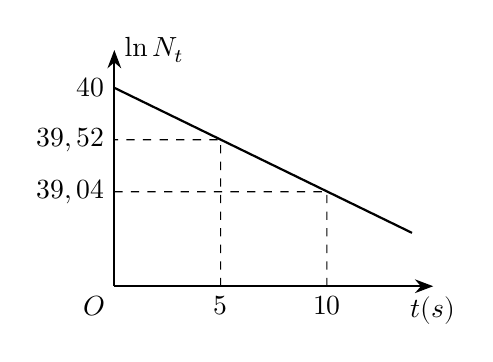
\begin{tikzpicture}[>=Stealth, scale=0.6, xscale=1.5]
            % 1. Vẽ hệ trục tọa độ
            \draw[->, thick] (0, 0) -- (4.5, 0) node[below] {$t(s)$};
            \draw[->, thick] (0, 0) -- (0, 5) node[right] {$\ln N_t$};
            
            % 2. Gốc tọa độ O
            \node[below left] at (0, 0) {$O$};
            
            % 3. Định nghĩa các điểm chính cho đồ thị
            % (Sử dụng tọa độ (X, Y) để mô phỏng tỉ lệ thực tế)
            \coordinate (P0) at (0, 4.2);      % Ứng với giá trị 40
            \coordinate (P1) at (1.5, 3.1);    % Ứng với t=5, lnN=39,52
            \coordinate (P2) at (3.0, 2.0);    % Ứng với t=10, lnN=39,04

            % 4. Vẽ đường thẳng đồ thị
            \draw[thick] (P0) -- (4.2, 1.13);

            % 5. Vẽ các đường dóng (dashed lines)
            \draw[dashed] (1.5, 0) -- (P1) -- (0, 3.1);
            \draw[dashed] (3.0, 0) -- (P2) -- (0, 2.0);

            % 6. Thêm các nhãn số trên trục tung
            \node[left] at (P0) {$40$};
            \node[left] at (0, 3.1) {$39,52$};
            \node[left] at (0, 2.0) {$39,04$};

            % 7. Thêm các nhãn số trên trục hoành
            \node[below] at (1.5, 0) {$5$};
            \node[below] at (3.0, 0) {$10$};

        \end{tikzpicture}
    }
    \shortans{18}
    \loigiai{
        $N_t = N_0 \cdot 2^{-\frac{t}{T}} \Rightarrow \left\{\begin{aligned} & e^{40} = N_0 \cdot 2^0 \\ & e^{39{,}52} = N_0 \cdot 2^{-\frac{5}{T}} \end{aligned}\right. \Rightarrow 2^{-\frac{5}{T}} = \frac{e^{39{,}52}}{e^{40}}$ \\
        $\Delta N = N_0 \left(1 - 2^{-\frac{15}{T}}\right) = e^{40} \cdot \left[1 - \left(\frac{e^{39{,}52}}{e^{40}}\right)^3\right] \approx {18 \cdot 10^{16}}$.
    }
\end{ex}
% Câu 1
\begin{ex}
    Số nucleon mang điện có trong hạt nhân ${}_{11}^{23}\mathrm{Na}$ là
    \choice
    {${34}$}
    {${12}$}
    {\True ${11}$}
    {${23}$}
    \loigiai{
        ${Z = 11}$
    }
\end{ex}


% Câu 2
\begin{ex}
    Cho phản ứng hạt nhân: ${}_{1}^{2}\mathrm{H} + {}_{1}^{2}\mathrm{H} \rightarrow {}_{2}^{4}\mathrm{He}$. Đây là
    \choice
    {phản ứng phân hạch}
    {\True phản ứng nhiệt hạch}
    {phản ứng thu năng lượng}
    {hiện tượng phóng xạ hạt nhân}
    \loigiai{
    }
\end{ex}


% Câu 3
\begin{ex}
    Khi hai vật ${A}$ và ${B}$ tiếp xúc nhau thì nguyên nhân ${A}$ truyền nhiệt cho ${B}$ là
    \choice
    {\True nhiệt độ của ${A}$ lớn hơn của ${B}$}
    {nhiệt dung riêng của ${A}$ lớn hơn của ${B}$}
    {nội năng của ${A}$ lớn hơn của ${B}$}
    {khối lượng của ${A}$ lớn hơn của ${B}$}
    \loigiai{
    }
\end{ex}


% Câu 4
\begin{ex}
    Trong từ trường đều có cường độ từ trường ${B}$, độ lớn từ thông đi qua một mặt hình chữ nhật có diện tích ${S}$ không thể là
    \choice
    {${0}$}
    {${BS}$}
    {${ \frac{2}{3} BS }$}
    {\True ${ \frac{3}{2} BS }$}
    \loigiai{
        ${\phi = BS \cos \alpha \le BS}$
    }
\end{ex}


% Câu 5
\begin{ex}
    Kết luận nào sau đây đúng về lực tương tác giữa các phân tử?
    \choice
    {Lực hút phân tử mạnh lên khi khoảng cách giữa các phân tử tăng}
    {\True Lực đẩy phân tử mạnh lên khi khoảng cách giữa các phân tử giảm}
    {Hợp lực tương tác phân tử có độ lớn tăng khi khoảng cách giữa các phân tử tăng}
    {Hợp lực tương tác phân tử có độ lớn tăng khi khoảng cách giữa các phân tử giảm}
    \loigiai{
    }
\end{ex}


% Câu 6
\begin{ex}
    Với một lượng khí lí tưởng nhất định, phát biểu nào sau đây là đúng?
    \choice
    {\True Khi áp suất tăng và thể tích tăng, thì động năng trung bình của các phân tử cũng tăng}
    {Khi áp suất giảm và thể tích giảm, thì động năng trung bình của các phân tử tăng}
    {Khi áp suất giảm và thể tích tăng, thì động năng trung bình của các phân tử tăng}
    {Khi áp suất tăng và thể tích giảm, thì động năng trung bình của các phân tử tăng}
    \loigiai{
        ${pV = nRT \xrightarrow{pV \uparrow} T \uparrow \Rightarrow W_d \uparrow}$
    }
\end{ex}


% Câu 7
\begin{ex}
    Nhiệt độ ${100^\circ\mathrm{C}}$ tương đương với nhiệt độ nhiệt động
    \choice
    {\True ${373 \, \mathrm{K}}$}
    {${-173 \, \mathrm{K}}$}
    {${273 \, \mathrm{K}}$}
    {${173 \, \mathrm{K}}$}
    \loigiai{
        ${T(\mathrm{K}) = t(^\circ\mathrm{C}) + 273 = 100 + 273 = 373(\mathrm{K})}$
    }
\end{ex}


% Câu 8
\begin{ex}
    Trong quá trình nén một lượng khí, khí nhận công ${1{,}2 \cdot 10^5 \, \mathrm{J}}$ và nội năng khí tăng thêm ${8 \cdot 10^4 \, \mathrm{J}}$. Lượng khí này đã
    \choice
    {tỏa nhiệt lượng ${2 \cdot 10^5 \, \mathrm{J}}$}
    {nhận nhiệt lượng ${4 \cdot 10^4 \, \mathrm{J}}$}
    {\True tỏa nhiệt lượng ${4 \cdot 10^4 \, \mathrm{J}}$}
    {nhận nhiệt lượng ${2 \cdot 10^5 \, \mathrm{J}}$}
    \loigiai{
        ${\Delta U = A + Q \Rightarrow 8 \cdot 10^4 = 1{,}2 \cdot 10^5 + Q \Rightarrow Q = -4 \cdot 10^4 \, \mathrm{J}}$
    }
\end{ex}


% Câu 9
\begin{ex}
    Trong quá trình đẳng áp, nhiệt độ của một lượng khí nhất định tăng từ ${7^\circ\mathrm{C}}$ lên ${147^\circ\mathrm{C}}$ thì thể tích của nó tăng lên bao nhiêu lần?
    \choice
    {${21}$}
    {\True ${1{,}5}$}
    {${5{,}7}$}
    {${7}$}
    \loigiai{
        Đẳng áp ${\Rightarrow \frac{V_1}{T_1} = \frac{V_2}{T_2} \Rightarrow \frac{V_2}{V_1} = \frac{T_2}{T_1} = \frac{147 + 273}{7 + 273} = 1{,}5}$
    }
\end{ex}


% Câu 10
\begin{ex}
    Khối lượng của proton, neutron và hạt nhân ${}_{18}^{37}\mathrm{Ar}$ lần lượt là ${1{,}0073 \, \mathrm{amu}}$; ${1{,}0087 \, \mathrm{amu}}$; ${36{,}9565 \, \mathrm{amu}}$. Độ hụt khối của hạt nhân ${}_{18}^{37}\mathrm{Ar}$ là
    \choice
    {${0{,}3132 \, \mathrm{amu}}$}
    {${0{,}3650 \, \mathrm{amu}}$}
    {\True ${0{,}3402 \, \mathrm{amu}}$}
    {${0{,}3384 \, \mathrm{amu}}$}
    \loigiai{
        ${\Delta m = Z m_p + (A - Z) m_n - m = 18 \cdot 1{,}0073 + (37 - 18) \cdot 1{,}0087 - 36{,}9565 = 0{,}3402 \, \mathrm{amu}}$
    }
\end{ex}


% Câu 11
\begin{ex}
    Một lượng khí lí tưởng nhất định có thể tích không đổi, ban đầu ở nhiệt độ ${27^\circ\mathrm{C}}$. Nếu áp suất của khí giảm đi một nửa thì nhiệt độ của khí là
    \choice
    {${127 \, \mathrm{K}}$}
    {\True ${150 \, \mathrm{K}}$}
    {${13{,}5^\circ\mathrm{C}}$}
    {${-23{,}5^\circ\mathrm{C}}$}
    \loigiai{
        ${\frac{p_1}{T_1} = \frac{p_2}{T_2} \Rightarrow \frac{2}{27 + 273} = \frac{1}{T_2} \Rightarrow T_2 = 150 \, \mathrm{K}}$
    }
\end{ex}


% Câu 12
\begin{ex}
    Xét một sóng điện từ có phương truyền thẳng đứng hướng lên. Biết cường độ điện trường cực đại là ${E_0}$ và cảm ứng từ cực đại là ${B_0}$. Vào thời điểm ${t}$, tại điểm ${M}$ trên phương truyền, vectơ cường độ điện trường đang có độ lớn ${\frac{1}{2} E_0}$ và hướng về phía Nam. Khi đó, vectơ cảm ứng từ có
    \choice
    {\True độ lớn ${\frac{1}{2} B_0}$ và hướng về phía Đông}
    {độ lớn ${\frac{\sqrt{3}}{2} B_0}$ và hướng về phía Đông}
    {độ lớn ${\frac{1}{2} B_0}$ và hướng về phía Tây}
    {độ lớn ${\frac{\sqrt{3}}{2} B_0}$ và hướng về phía Tây}
    \loigiai{
        ${\frac{B}{B_0} = \frac{E}{E_0} = \frac{1}{2}}$. Áp dụng quy tắc tam diện thuận
    }
\end{ex}


% Câu 13
\begin{ex}
    Một lốp ô tô có thể tích ${30}$ lít chứa không khí (được coi là lí tưởng) ở nhiệt độ ${27^\circ\mathrm{C}}$ và áp suất ${2{,}4 \cdot 10^5 \, \mathrm{Pa}}$. Số phân tử không khí có trong lốp ô tô này là
    \choice
    {${1{,}7 \cdot 10^{23}}$}
    {\True ${1{,}7 \cdot 10^{24}}$}
    {${8 \cdot 10^{23}}$}
    {${8 \cdot 10^{24}}$}
    \loigiai{
        ${n = \frac{pV}{RT} = \frac{2{,}4 \cdot 10^5 \cdot 30 \cdot 10^{-3}}{8{,}31 \cdot (27 + 273)} \approx 2{,}888 \, \mathrm{mol}}$. \\
        ${N = n N_A = 2{,}888 \cdot 6{,}02 \cdot 10^{23} \approx 1{,}7 \cdot 10^{24}}$
    }
\end{ex}


% Câu 14
\begin{ex}
    Biết ${}_{84}^{210}\mathrm{Po}$ phóng xạ ${\alpha}$ và biến thành hạt nhân chì với chu kì bán rã ${138}$ ngày. Tại ${t = 0}$, một mẫu ${}_{84}^{210}\mathrm{Po}$ nguyên chất có khối lượng ${10 \, \mathrm{g}}$. Sau ${2}$ năm (một năm lấy ${365}$ ngày), khối lượng chì tạo thành trong mẫu là
    \choice
    {${8{,}11 \, \mathrm{g}}$}
    {${9{,}74 \, \mathrm{g}}$}
    {${6{,}23 \, \mathrm{g}}$}
    {\True ${9{,}56 \, \mathrm{g}}$}
    \loigiai{
        ${}_{84}^{210}\mathrm{Po} \rightarrow {}_2^4\alpha + {}_{82}^{206}\mathrm{Pb}$. \\
        ${m_{\mathrm{Pb}} = m_0 \cdot \frac{A_{\mathrm{Pb}}}{A_{\mathrm{Po}}} \cdot \left( 1 - 2^{-\frac{t}{T}} \right) = 10 \cdot \frac{206}{210} \cdot \left( 1 - 2^{-\frac{2 \cdot 365}{138}} \right) \approx 9{,}56 \, \mathrm{g}}$
    }
\end{ex}


% Câu 15
\begin{ex}
    Hai chất phóng xạ $A$ và $B$ có hằng số phóng xạ lần lượt là ${10\lambda}$ và ${\lambda}$. Thời điểm ${t = 0}$, số hạt nhân của hai chất phóng xạ này bằng nhau. Thời điểm mà tỉ số hạt nhân của $A$ so với hạt nhân của $B$ bằng ${\frac{1}{e}}$ (với ${\ln e = 1}$) là
    \choice
    {${ \frac{1}{11\lambda} }$}
    {${ \frac{11}{10\lambda} }$}
    {${ \frac{1}{10\lambda} }$}
    {\True ${ \frac{1}{9\lambda} }$}
    \loigiai{
        ${N = N_0 e^{-\lambda t} \Rightarrow \frac{N_A}{N_B} = \frac{e^{-10\lambda t}}{e^{-\lambda t}} = e^{-9\lambda t} = \frac{1}{e} \Rightarrow 9\lambda t = 1 \Rightarrow t = \frac{1}{9\lambda}}$
    }
\end{ex}


% Câu 16
\begin{ex}
\immini[thm]{
    Giác hơi là một phương pháp điều trị trong y học cổ truyền. Trong quá trình giác hơi, bác sĩ làm nóng không khí trong cốc đến nhiệt độ ${t \, (^\circ\mathrm{C})}$ nhất định, sau đó nhanh chóng lật ngược cốc úp xuống da. Khi nhiệt độ giảm xuống nhiệt độ phòng là ${27^\circ\mathrm{C}}$, áp suất khí trong cốc bằng ${0{,}8}$ lần áp suất khí quyển. Coi lượng khí kín trong cốc là khí lí tưởng, bỏ qua sự thay đổi thể tích. Giá trị của ${t}$ là
}{
    \includegraphics[width=0.22\linewidth]{extracted_figures/fig_p2_3_scale0.24.png}
}
    \choice
    {${87}$}
    {\True ${102}$}
    {${207}$}
    {${227}$}
    \loigiai{
        ${\frac{p}{T} = \mathrm{const} \Rightarrow \frac{p_0}{t + 273} = \frac{0{,}8 p_0}{27 + 273} \Rightarrow t \approx 102^\circ\mathrm{C}}$
    }
\end{ex}


% Câu 17
\begin{ex}
    Áp suất lốp là một thông số quan trọng phải lưu tâm để lái xe an toàn. Thể tích lốp của một ô tô là ${25}$ lít và phạm vi áp suất lốp an toàn là từ ${2{,}4 \, \mathrm{atm}}$ đến ${3{,}0 \, \mathrm{atm}}$. Sau khi ô tô chạy một thời gian, người lái xe thấy áp suất lốp giảm xuống ${2{,}0 \, \mathrm{atm}}$ nên sử dụng máy bơm không khí trên xe có tốc độ bơm là ${0{,}5}$ lít khí ở áp suất ${1{,}0 \, \mathrm{atm}}$ mỗi giây. Bỏ qua sự thay đổi thể tích lốp và nhiệt độ khí. Khoảng thời gian bơm không khí để đưa áp suất lốp về mức an toàn là
    \choice
    {từ ${120 \, \mathrm{s}}$ đến ${150 \, \mathrm{s}}$}
    {từ ${60 \, \mathrm{s}}$ đến ${75 \, \mathrm{s}}$}
    {từ ${40 \, \mathrm{s}}$ đến ${100 \, \mathrm{s}}$}
    {\True từ ${20 \, \mathrm{s}}$ đến ${50 \, \mathrm{s}}$}
    \loigiai{
        ${n_s = n_t + n_b \xrightarrow{n = \frac{pV}{RT}} p_s V = p_t V + p_b V_b \Rightarrow p_s \cdot 25 = 2 \cdot 25 + 1 \cdot 0{,}5t \xrightarrow{2{,}4 \le p_s \le 3} 20 \, \mathrm{s} \le t \le 50 \, \mathrm{s}}$
    }
\end{ex}


% Câu 18
\begin{ex}
    Hạt nhân bo ${}_5^{10}\mathrm{B}$ đang đứng yên thì hấp thụ một neutron chậm (tốc độ không đáng kể), sau đó thu được hạt nhân liti ${}_3^7\mathrm{Li}$ và hạt X. Biết động năng hạt X thu được là ${1{,}8 \, \mathrm{MeV}}$. Phản ứng này
    \choice
    {\True tỏa ${2{,}83 \, \mathrm{MeV}}$}
    {thu ${2{,}83 \, \mathrm{MeV}}$}
    {tỏa ${4{,}95 \, \mathrm{MeV}}$}
    {thu ${4{,}95 \, \mathrm{MeV}}$}
    \loigiai{
        ${}_5^{10}\mathrm{B} + {}_0^1\mathrm{n} \rightarrow {}_3^7\mathrm{Li} + {}_2^4\mathrm{X}$. \\
        ${p_{\mathrm{Li}}^2 = p_{\mathrm{X}}^2 \Rightarrow 2m_{\mathrm{Li}} K_{\mathrm{Li}} = 2m_{\mathrm{X}} K_{\mathrm{X}} \Rightarrow 7 K_{\mathrm{Li}} = 4 \cdot 1{,}8 \Rightarrow K_{\mathrm{Li}} \approx 1{,}03 \, \mathrm{MeV}}$. \\
        ${\Delta E = K_{\mathrm{Li}} + K_{\mathrm{X}} = 1{,}03 + 1{,}8 = 2{,}83 \, \mathrm{MeV}}$
    }
\end{ex}


% Câu 1
\begin{ex}
    Một nhóm học sinh làm thí nghiệm xác định nhiệt nóng chảy riêng của nước đá với bộ dụng cụ gồm: Nhiệt lượng kế có nắp kín và đáy có lỗ hở, biến áp nguồn, dây nung công suất ${P = 12 \, \mathrm{W}}$; cân điện tử; cốc hứng nước; giá đỡ. Bố trí thí nghiệm như hình vẽ, tiến hành và quan sát thí nghiệm qua hai giai đoạn liên tiếp:
    \begin{center}
        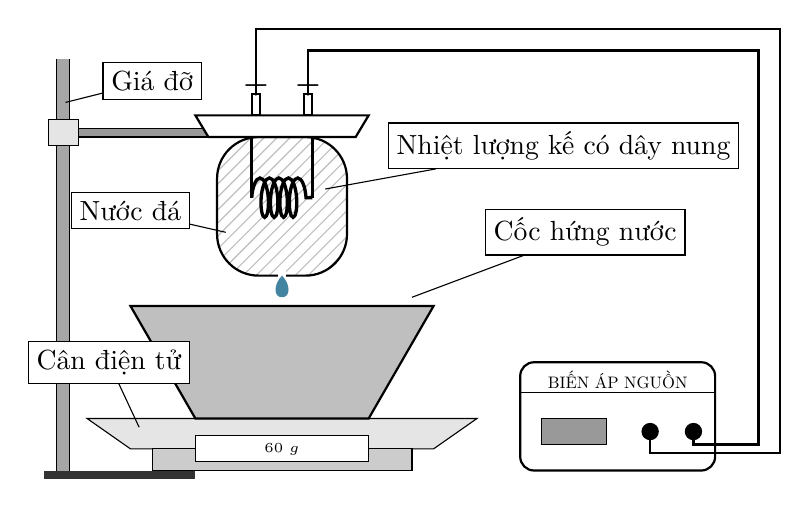
\begin{tikzpicture}[scale=0.55]
            % --- Giá đỡ (Support Stand) ---
            \fill[black!80] (0, -0.2) rectangle (3.5, 0); % Đế
            \fill[gray!70] (0.3, 0) rectangle (0.6, 9.5); % Trụ đứng
            \draw (0.3, 0) -- (0.3, 9.5) (0.6, 0) -- (0.6, 9.5);
            \draw[fill=gray!20] (0.1, 7.5) rectangle (0.8, 8.1); % Khớp nối
            \draw[fill=gray!80] (0.8, 7.7) rectangle (4.5, 7.9); % Thanh ngang
            
            % --- Nhiệt lượng kế (Calorimeter) ---
            % Thân bình và Nước đá (Sử dụng mẫu gạch chéo để mô phỏng đá)
            \begin{scope}
                \clip[rounded corners=15pt] (4, 4.5) rectangle (7, 7.7);
                \foreach \i in {0,0.3,...,4} \draw[lightgray, thin] (3.5+\i, 4.0) -- (7.5, 8.0-\i);
                \foreach \i in {0,0.3,...,4} \draw[lightgray, thin] (3.5, 4.0+\i) -- (7.5-\i, 8.0);
            \end{scope}
            \draw[thick, rounded corners=15pt] (4, 4.5) rectangle (7, 7.7);
            
            % Nắp và các cực điện
            \draw[fill=white, thick] (3.8, 7.7) -- (7.2, 7.7) -- (7.5, 8.2) -- (3.5, 8.2) -- cycle;
            \draw[thick] (4.8, 8.2) rectangle (5.0, 8.7); % Cực trái
            \draw[thick] (6.0, 8.2) rectangle (6.2, 8.7); % Cực phải
            \node at (4.9, 8.9) {\textbf{+}};
            \node at (6.1, 8.9) {\textbf{+}};
            
            % Dây nung (Heating coil)
            \draw[decoration={aspect=0.3, segment length=1.2mm, amplitude=2.5mm, coil}, decorate, line width=1.2pt] (4.8, 6.3) -- (6.2, 6.3);
            \draw[line width=1.2pt] (4.8, 6.3) -- (4.8, 7.7);
            \draw[line width=1.2pt] (6.2, 6.3) -- (6.2, 7.7);
            
            % Lỗ thoát và giọt nước
            \draw[thick, white, line width=3pt] (5.4, 4.5) -- (5.6, 4.5); 
            \fill[cyan!60!black] (5.5, 4.5) .. controls (5.3, 4.3) and (5.3, 4) .. (5.5, 4) .. controls (5.7, 4) and (5.7, 4.3) .. (5.5, 4.5) -- cycle;
            
            % --- Cân điện tử & Cốc hứng (Scale & Beaker) ---
            % Cân điện tử
            \draw[fill=gray!20] (2, 0.5) -- (9, 0.5) -- (10, 1.2) -- (1, 1.2) -- cycle; % Bàn cân
            \draw[fill=gray!40] (2.5, 0) rectangle (8.5, 0.5); % Thân cân
            \draw[fill=white] (3.5, 0.2) rectangle (7.5, 0.8); % Màn hình
            \node at (5.5, 0.5) {\tiny {\textifsym{60}} ${g}$};
            
            % Cốc hứng nước
            \draw[fill=gray!50, thick] (3.5, 1.2) -- (7.5, 1.2) -- (9, 3.8) -- (2, 3.8) -- cycle;
            
            % --- Biến áp nguồn (Power supply) ---
            \draw[rounded corners=5pt, fill=white, thick] (11, 0) rectangle (15.5, 2.5);
            \draw (11, 1.8) -- (15.5, 1.8);
            \node at (13.25, 2.1) [scale=0.6] {BIẾN ÁP NGUỒN};
            \draw[fill=gray!80] (11.5, 0.6) rectangle (13.0, 1.2);
            \fill (14, 0.9) circle (0.2);
            \fill (15, 0.9) circle (0.2);
            
            % Dây dẫn (Wires)
            \draw[thick] (14, 0.9) -- (14, 0.4) -- (17, 0.4) -- (17, 10.2) -- (4.9, 10.2) -- (4.9, 8.7);
            \draw[thick] (15, 0.9) -- (15, 0.6) -- (16.5, 0.6) -- (16.5, 9.7) -- (6.1, 9.7) -- (6.1, 8.7);
            
            % --- Chú thích (Labels) ---
            \tikzset{lbl/.style={draw, fill=white, inner sep=3pt}}
            \node[lbl] (GL) at (2.5, 9) {Giá đỡ}; \draw (GL) -- (0.5, 8.5);
            \node[lbl] (NLK) at (12, 7.5) {Nhiệt lượng kế có dây nung}; \draw (NLK) -- (6.5, 6.5);
            \node[lbl] (ND) at (2, 6) {Nước đá}; \draw (ND) -- (4.2, 5.5);
            \node[lbl] (CH) at (12.5, 5.5) {Cốc hứng nước}; \draw (CH) -- (8.5, 4);
            \node[lbl] (CDT) at (1.5, 2.5) {Cân điện tử}; \draw (CDT) -- (2.2, 1);
        \end{tikzpicture}
    \end{center}
    \textbf{Giai đoạn 1:} Cho khối nước đá đang tan vào nhiệt lượng kế, bật nguồn điện để dây nung nóng lên làm nước đá nóng chảy, cốc hứng nước đặt trên cân điện tử hứng nước chảy ra từ nhiệt lượng kế và quan sát số chỉ của cân. Sau một thời gian kể từ khi cấp điện cho dây nung, tại thời điểm ${t_1}$, thấy số chỉ của cân là ${40 \, \mathrm{g}}$.\\
    \textbf{Giai đoạn 2:} Tiếp tục quan sát thì nhận thấy, sau thời gian ${10}$ phút kế tiếp kể từ thời điểm ${t_1}$, số chỉ của cân tăng đến ${60 \, \mathrm{g}}$.\\
    Coi rằng toàn bộ nhiệt lượng tỏa ra từ dây nung đều truyền cho nước đá và toàn bộ nước đá tan ra đều chảy vào cốc, bỏ qua sự trao đổi nhiệt với nhiệt lượng kế và môi trường, bỏ qua các ảnh hưởng khác (bay hơi, ngưng tụ của nước,...).
    \choiceTF[1]
    {\True Theo phương án thí nghiệm, nhiệt nóng chảy riêng của nước đá ở nhiệt độ nóng chảy là ${3{,}6 \cdot 10^5 \, \mathrm{J/kg}}$}
    {Quá trình nước đá nóng chảy là quá trình tỏa nhiệt}
    {Phương án thí nghiệm này là một trong những phương án có thể loại bỏ ảnh hưởng của sự trao đổi nhiệt với môi trường đến kết quả thí nghiệm}
    {Số chỉ của cân là khối lượng của nước đá đã nóng chảy và chảy vào cốc hứng}
    \loigiai{
        \begin{itemchoice}
        \itemch ${\lambda = \frac{Pt}{\Delta m} = \frac{12 \cdot 10 \cdot 60}{(60 - 40) \cdot 10^{-3}} = 3{,}6 \cdot 10^5 \, \mathrm{J/kg}}$
        \itemch Nước đá nóng chảy là quá trình thu nhiệt
        \itemch Nước đá không cần bật dây nung nó có thể tự tan chảy được. Phương án thí nghiệm này là một trong những phương án không thể loại bỏ. Phải quan sát giai đoạn để đá tự chảy ra khi nó trao đổi nhiệt với môi trường
        \itemch Số chỉ của cân bao gồm khối lượng của cốc và khối lượng của nước đá đã nóng chảy, chảy vào cốc ${\Rightarrow}$ Số chỉ của cân là khối lượng của nước đá đã nóng chảy và chảy vào cốc ${+ m_{\mathrm{cốc}}}$
        \end{itemchoice}
    }
\end{ex}


% Câu 3
\begin{ex}
\immini[thm]{
    Hình vẽ mô tả thí nghiệm đo độ lớn của cảm ứng từ $B$. Khung dây dẫn $ABCD$ được gắn vào một cánh tay đòn $OM$ của cân và được treo sao cho mặt phẳng khung vuông góc với vectơ cảm ứng từ của từ trường đều. Ban đầu, dòng điện trong khung dây bằng không, cân ở trạng thái cân bằng, đòn cân $MN$ nằm ngang. Khi cho dòng điện có cường độ ${I = 1{,}0 \, \mathrm{A}}$ chạy qua khung dây thì cần thêm quả cân có khối lượng ${20 \, \mathrm{g}}$ vào đĩa cân bên phải để cân trở lại trạng thái cân bằng, đòn cân $MN$ nằm ngang. Khung dây hình chữ nhật $ABCD$ gồm ${20}$ vòng dây có chiều rộng ${AB = a = 5{,}0 \, \mathrm{cm}}$. Lấy ${g = 9{,}8 \, \mathrm{m/s^2}}$.
}{
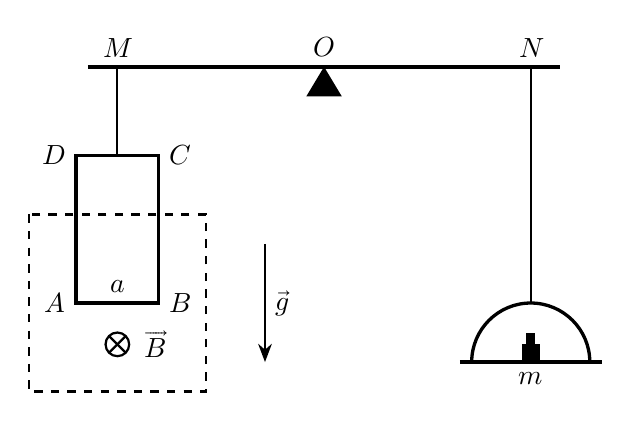
\begin{tikzpicture}[>=Stealth, scale=0.75]
    % 1. Thanh ngang (Beam)
    \draw[ultra thick] (-4, 0) -- (4, 0);
    \node at (-3.5, 0) [above] {$M$};
    \node at (0, 0) [above] {$O$};
    \node at (3.5, 0) [above] {$N$};

    % 2. Điểm tựa (Fulcrum)
    \fill (0, 0) -- (-0.3, -0.5) -- (0.3, -0.5) -- cycle;

    % 3. Phía trái: Khung dây ABCD
    % Dây treo từ M
    \draw[thick] (-3.5, 0) -- (-3.5, -1.5);
    % Hình chữ nhật ABCD
    \draw[very thick] (-4.2, -1.5) node[left] {$D$} -- (-2.8, -1.5) node[right] {$C$} -- (-2.8, -4) node[right] {$B$} -- (-4.2, -4) node[left] {$A$} -- cycle;
    % Nhãn độ dài cạnh đáy 'a'
    \node at (-3.5, -4) [above] {$a$};

    % 4. Vùng từ trường (Magnetic Field Region)
    \draw[thick, dashed] (-5, -2.5) rectangle (-2, -5.5);
    % Ký hiệu B hướng vào trang giấy
    \begin{scope}[shift={(-3.5, -4.7)}]
        \draw[thick] (0,0) circle (0.2);
        \draw[thick] (-0.14, -0.14) -- (0.14, 0.14);
        \draw[thick] (-0.14, 0.14) -- (0.14, -0.14);
        \node at (0.3, 0) [right] {$\overrightarrow{B}$};
    \end{scope}

    % 5. Vectơ gia tốc trọng trường g
    \draw[->, thick] (-1, -3) -- (-1, -5) node[right, midway] {$\overrightarrow{g}$};

    % 6. Phía phải: Đĩa cân và khối lượng m
    % Dây treo từ N
    \draw[thick] (3.5, 0) -- (3.5, -4);
    % Đĩa cân (Pan)
    \begin{scope}[shift={(3.5, -4)}]
        \draw[very thick] (-1, -1) arc (180:0:1); % Quai cân hình cung
        \draw[ultra thick] (-1.2, -1) -- (1.2, -1); % Đế cân
        % Khối lượng m
        \fill[black] (-0.08, -0.7) rectangle (0.08, -0.5);
        \fill[black] (-0.15, -1) rectangle (0.15, -0.7);
        \node at (0, -1) [below] {$m$};
    \end{scope}

\end{tikzpicture}
}
    \choiceTF[1]
    {Lực từ tác dụng vào khung dây ngược hướng với trọng lực của nó}
    {\True Dòng điện $I$ chạy trong khung dây có chiều từ $B$ tới $A$}
    {\True Độ lớn của lực từ tác dụng vào khung $ABCD$ là ${196 \, \mathrm{mN}}$}
    {\True Độ lớn của cảm ứng từ ${B = 196 \, \mathrm{mT}}$}
    \loigiai{
        \begin{itemchoice}
        \itemch Cân ở trạng thái cân bằng ${\Rightarrow}$ lực từ hướng xuống, cùng hướng trọng lực
        \itemch Áp dụng quy tắc bàn tay trái ${\Rightarrow I}$ có chiều từ $B$ tới $A$
        \itemch ${F = mg = 20 \cdot 10^{-3} \cdot 9{,}8 = 0{,}196 \, \mathrm{N} = 196 \, \mathrm{mN}}$
        \itemch ${F = NIBL \Rightarrow 0{,}196 = 20 \cdot 1 \cdot B \cdot 0{,}05 \Rightarrow B = 0{,}196 \, \mathrm{T} = 196 \, \mathrm{mT}}$
        \end{itemchoice}
    }
\end{ex}


% Câu 2
\begin{ex}
    Khi tia vũ trụ đi vào khí quyển Trái Đất và tương tác với khí quyển, chúng sẽ tạo ra neutron. Các neutron và nitơ 14 trong khí quyển sẽ tương tác gây ra phản ứng sau: ${}_7^{14}\mathrm{N} + {}_0^1\mathrm{n} \rightarrow {}_6^{14}\mathrm{C} + {}_1^1\mathrm{p}$. Đồng vị ${}_6^{14}\mathrm{C}$ được tạo ra có thể tự phân rã ${\beta^-}$ với chu kì bán rã là ${5730}$ năm. Quy luật phân rã của cacbon 14 được sử dụng để ước tính tuổi của gỗ cổ. Một mảnh gỗ cổ có số phân rã của ${}_6^{14}\mathrm{C}$ trong một giờ là ${650}$. Biết mảnh gỗ cùng khối lượng của cây cùng loại khi mới chặt có số phân rã của ${}_6^{14}\mathrm{C}$ trong một giờ là ${2600}$.
    \choiceTF[1]
    {Sản phẩm phân rã ${\beta^-}$ của ${}_6^{14}\mathrm{C}$ là ${}_7^{15}\mathrm{N}$}
    {Electron phát ra từ ${}_6^{14}\mathrm{C}$ trong phân rã là từ các electron ngoài hạt nhân trong nguyên tử cacbon}
    {Trong những năm gần đây, chu kì bán rã của ${}_6^{14}\mathrm{C}$ đã có chút thay đổi}
    {\True Tuổi của mảnh gỗ cổ là ${11460}$ năm}
    \loigiai{
        \begin{itemchoice}
        \itemch ${}_6^{14}\mathrm{C} \rightarrow {}_{-1}^0\mathrm{e} + {}_7^{14}\mathrm{X}$
        \itemch Electron phát ra từ phân rã ${\beta^-}$ là electron hạt nhân, không phải electron ngoài hạt nhân
        \itemch Chu kì bán rã không thay đổi
        \itemch ${H = H_0 \cdot 2^{-\frac{t}{T}} \Rightarrow 650 = 2600 \cdot 2^{-\frac{t}{5730}} \Rightarrow t = 11460}$ năm
        \end{itemchoice}
    }
\end{ex}


% Câu 4
\begin{ex}
\immini[thm]{
    Một khối khí lí tưởng nhất định thay đổi trạng thái ${A \rightarrow B \rightarrow C}$ theo chiều mũi tên trên đồ thị ${p - T}$ ở hình bên. Biết thể tích của khí ở trạng thái $C$ là ${20}$ lít và trong toàn bộ quá trình khí thực hiện công là ${60 \, \mathrm{J}}$.
    \choiceTF[1]
    {\True Thể tích của khí ở trạng thái $B$ là ${15}$ lít}
    {Thể tích của khí ở trạng thái $A$ là ${5}$ lít}
    {\True Khí thu nhiệt trong quá trình ${A \rightarrow B}$}
    {Áp suất của khí ở trạng thái $B$ là ${4 \cdot 10^3 \, \mathrm{Pa}}$}
}{
    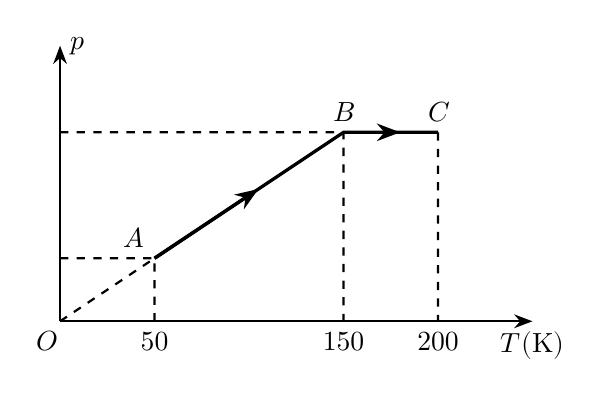
\begin{tikzpicture}[>=Stealth, thick, scale=1, xscale = 0.8]
        % --- 1. Vẽ hệ trục tọa độ ---
        \draw[->, thick] (0,0) -- (7.5,0) node[below] {$T \, \mathrm{(K)}$};
        \draw[->, thick] (0,0) -- (0,3.5) node[right] {$p$};
        \node at (-0.2, -0.25) {$O$};

        % --- 2. Định nghĩa các tọa độ điểm ---
        % Chọn tỉ lệ: 50K ứng với 1.5 đơn vị độ dài trên trục hoành
        \coordinate (A) at (1.5, 0.8);
        \coordinate (B) at (4.5, 2.4); % Đường AB kéo dài đi qua gốc O (p tỉ lệ với T)
        \coordinate (C) at (6.0, 2.4);

        % --- 3. Vẽ các đường dóng nét đứt ---
        \draw[dashed] (0,0) -- (A); % Phần kéo dài qua gốc O
        \draw[dashed] (0, 0.8) -- (A) -- (1.5, 0);
        \draw[dashed] (0, 2.4) -- (B) -- (4.5, 0);
        \draw[dashed] (C) -- (6.0, 0);

        % --- 4. Vẽ quá trình biến đổi (màu đỏ) ---
        \draw[very thick] (A) -- (B) -- (C);

        % --- 5. Vẽ mũi tên chỉ hướng quá trình ---
        % Mũi tên trên đoạn AB
        \draw[very thick, ->] (A) -- (3.15, 1.68); 
        % Mũi tên trên đoạn BC
        \draw[very thick, ->] (B) -- (5.4, 2.4);

        % --- 6. Thêm các nhãn văn bản ---
        \node[above left] at (A) {$A$};
        \node[above] at (B) {$B$};
        \node[above] at (C) {$C$};
        \node[below] at (1.5, 0) {50};
        \node[below] at (4.5, 0) {150};
        \node[below] at (6.0, 0) {200};
    \end{tikzpicture}
}
    \loigiai{
        \begin{itemchoice}
        \itemch $BC$ là đẳng áp ${\Rightarrow \frac{V_B}{T_B} = \frac{V_C}{T_C} \Rightarrow \frac{V_B}{150} = \frac{20}{200} \Rightarrow V_B = 15 \, \mathrm{l}}$
        \itemch $AB$ là đẳng tích ${\Rightarrow V_A = V_B = 15 \, \mathrm{l}}$
        \itemch $AB$ có công ${A = 0}$ và nhiệt độ tăng ${\Rightarrow}$ nội năng tăng ${\Rightarrow}$ thu nhiệt
        \itemch ${A_{BC}' = p_B (V_C - V_B) \Rightarrow 60 = p_B (20 - 15) \cdot 10^{-3} \Rightarrow p_B = 12 \cdot 10^3 \, \mathrm{Pa}}$
        \end{itemchoice}
    }
\end{ex}


% Câu 1
\begin{ex}
    Đun nóng ${600 \, \mathrm{g}}$ nước đến ${63^\circ\mathrm{C}}$ thì nhiệt lượng mà nước hấp thụ là ${3{,}78 \cdot 10^4 \, \mathrm{J}}$. Biết nhiệt dung riêng của nước là ${4200 \, \mathrm{J/(kg \cdot K)}}$. Nhiệt độ ban đầu của nước là bao nhiêu ${^\circ\mathrm{C}}$?
    \shortans{48}
    \loigiai{
        ${Q = mc\Delta t \Rightarrow 3{,}78 \cdot 10^4 = 0{,}6 \cdot 4200 \cdot (63 - t) \Rightarrow t = 48^\circ\mathrm{C}}$
    }
\end{ex}


% Câu 2
\begin{ex}
    Ban đầu, từ thông qua một khung dây kín là ${0{,}4 \, \mathrm{Wb}}$. Nếu từ thông tăng đều và sau khoảng thời gian ${0{,}2 \, \mathrm{s}}$, từ thông qua khung dây tăng gấp ${5}$ lần thì suất điện động cảm ứng qua khung có độ lớn là bao nhiêu $\mathrm{V}$?
    \shortans{8}
    \loigiai{
        ${e = \left| \frac{\Delta \phi}{\Delta t} \right| = \frac{5 \cdot 0{,}4 - 0{,}4}{0{,}2} = 8 \, \mathrm{V}}$
    }
\end{ex}


% Câu 3
\begin{ex}
    Một ấm điện khi hoạt động tiêu thụ điện năng với công suất $P$. Dùng ấm điện đun ${1{,}5 \, \mathrm{kg}}$ nước từ ${25^\circ\mathrm{C}}$ lên ${85^\circ\mathrm{C}}$ mất ${6}$ phút. Biết nhiệt dung riêng của nước là ${4200 \, \mathrm{J/(kg \cdot K)}}$ và hiệu suất của ấm điện là ${60\%}$. Giá trị của $P$ là bao nhiêu $\mathrm{W}$?
    \shortans{1750}
    \loigiai{
        ${Q = mc\Delta t = 1{,}5 \cdot 4200 \cdot (85 - 25) = 378000 \, \mathrm{J}}$\\
        ${A = \frac{Q}{H} = \frac{378000}{0{,}6} = 630000 \, \mathrm{J}}$\\
        ${P = \frac{A}{t} = \frac{630000}{6 \cdot 60} = 1750 \, \mathrm{W}}$
    }
\end{ex}


% Câu 4
\begin{ex}
    Một bình chứa ${120 \, \mathrm{g}}$ khí oxygen ở áp suất ${10 \, \mathrm{atm}}$ và nhiệt độ ${47^\circ\mathrm{C}}$. Do bình chứa bị rò rỉ khí nên sau một thời gian nhất định khí trong bình có áp suất ${6{,}25 \, \mathrm{atm}}$ và nhiệt độ ${27^\circ\mathrm{C}}$. Khối lượng của khí oxygen đã thoát khỏi bình là bao nhiêu gam?
    \shortans{40}
    \loigiai{
        ${pV = nRT = \frac{m}{M} RT \Rightarrow \frac{p_2}{p_1} = \frac{m_2}{m_1} \cdot \frac{T_2}{T_1} \Rightarrow \frac{6{,}25}{10} = \frac{m_2}{120} \cdot \frac{27 + 273}{47 + 273} \Rightarrow m_2 = 80 \, \mathrm{g}}$\\
        ${\Delta m = m_1 - m_2 = 120 - 80 = 40 \, \mathrm{g}}$
    }
\end{ex}


% Câu 5
\begin{ex}
    Giả sử, một nhà máy điện tổng hợp hạt nhân dùng nhiên liệu deuterium ${}_1^2\mathrm{D}$ theo phản ứng: ${{}_1^2\mathrm{D} + {}_1^2\mathrm{D} \rightarrow {}_2^4\mathrm{He}}$. Biết công suất phát điện là ${200 \, \mathrm{MW}}$ và hiệu suất chuyển hóa năng lượng hạt nhân thành điện năng là ${25\%}$. Biết khối lượng hạt nhân ${}_1^2\mathrm{D}$ và ${}_2^4\mathrm{He}$ lần lượt là ${2{,}0141 \, \mathrm{amu}}$ và ${4{,}0026 \, \mathrm{amu}}$. Nếu nhà máy hoạt động liên tục thì lượng deuterium ${}_1^2\mathrm{D}$ mà nhà máy cần dùng trong ${1}$ ngày bằng bao nhiêu kg (làm tròn kết quả đến chữ số hàng phần trăm)?
    \shortans{0,12}
    \loigiai{
        ${A = Pt = 200 \cdot 10^6 \cdot 24 \cdot 60 \cdot 60 = 1{,}728 \cdot 10^{13} \, \mathrm{J}}$\\
        ${Q = \frac{A}{H} = \frac{1{,}728 \cdot 10^{13}}{0{,}25} = 6{,}912 \cdot 10^{13} \, \mathrm{J}}$\\
        ${\Delta E = (2m_D - m_{He}) c^2 = (2 \cdot 2{,}0141 - 4{,}0026) \cdot 931{,}5 = 23{,}8464 \, \mathrm{MeV} = 3{,}82 \cdot 10^{-12} \, \mathrm{J}}$\\
        ${N = \frac{Q}{\Delta E} = \frac{6{,}912 \cdot 10^{13}}{3{,}82 \cdot 10^{-12}} = 1{,}81 \cdot 10^{25}}$\\
        ${N_D = 2N = 2 \cdot 1{,}81 \cdot 10^{25} = 3{,}62 \cdot 10^{25}}$\\
        ${n_D = \frac{N_D}{N_A} = \frac{3{,}62 \cdot 10^{25}}{6{,}02 \cdot 10^{23}} = 60 \, \mathrm{mol}}$\\
        ${m_D = n_D M = 60 \cdot 2 = 120 \, \mathrm{g} = 0{,}12 \, \mathrm{kg}}$
    }
\end{ex}


% Câu 6
\begin{ex}
\immini[thm]{
    Như hình bên, một bình hình trụ đặt thẳng đứng, thành bình nhẵn, piston cách nhiệt chia khí trong bình thành hai buồng $A$ và $B$ với cùng thể tích, nhiệt độ của khí đều bằng ${27^\circ\mathrm{C}}$, áp suất của khí $A$ là ${p_0}$ và áp suất của khí $B$ là ${2p_0}$. Bây giờ, giữ nhiệt độ của khí $A$ không đổi đồng thời đun nóng khí ở phần $B$ để piston dâng lên cho đến khi thể tích của khí $A$ bằng ${\frac{2}{3}}$ giá trị ban đầu. Nhiệt độ của khí $B$ là bao nhiêu $\mathrm{K}$ (làm tròn kết quả đến chữ số hàng đơn vị)?
}{
    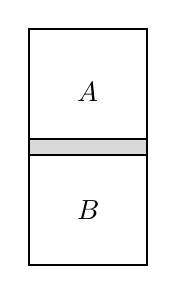
\begin{tikzpicture}[>={Stealth[length=8pt, width=6pt]}]
        \draw[thick] (0,3) -- (0,0) -- (1.5,0) -- (1.5,3) -- cycle;;
        \draw[thick, fill=gray!30] (0,1.4) -- (1.5,1.4) -- (1.5,1.6) -- (0,1.6) -- cycle;
        \node at (0.75,2.2) {$A$};
        \node at (0.75,0.7) {$B$};
    \end{tikzpicture}
}
    \shortans{500}
    \loigiai{
        Áp suất do trọng lượng piston nén xuống là ${p_B - p_A = 2p_0 - p_0 = p_0}$.
        \begin{center}
        \begin{tabular}{|l|l|l|l|}
        \hline
         & ${p}$ & ${V}$ & ${T}$ \\ \hline
        Buồng $A$ ban đầu & ${p_0}$ & ${V}$ & ${27 + 273 = 300 \, \mathrm{K}}$ \\ \hline
        Buồng $B$ ban đầu & ${2p_0}$ & ${V}$ & ${27 + 273 = 300 \, \mathrm{K}}$ \\ \hline
        Buồng $A$ lúc sau & ${p_A}$ & ${\frac{2V}{3}}$ & ${300 \, \mathrm{K}}$ \\ \hline
        Buồng $B$ lúc sau & ${p_A + p_0}$ & ${2V - \frac{2V}{3} = \frac{4V}{3}}$ & ${T}$ \\ \hline
        \end{tabular}
        \end{center}
        Buồng $A$ đẳng nhiệt ${\Rightarrow p_0 V = p_A \cdot \frac{2V}{3} \Rightarrow p_A = 1{,}5 p_0}$.\\
        Buồng $B$ có ${\frac{pV}{T} = \mathrm{const} \Rightarrow \frac{2p_0 V}{300} = \frac{(p_A + p_0) \cdot \frac{4V}{3}}{T} \xrightarrow{p_A = 1{,}5 p_0} T = 500 \, \mathrm{K}}$
    }
\end{ex}
% Câu 1
\begin{ex}
    Trong ba loại tia phóng xạ ${\alpha}$, ${\beta}$ và ${\gamma}$; tia đâm xuyên mạnh nhất và tia làm ion hóa mạnh nhất lần lượt là
    \choice
    {tia ${\alpha}$ và tia ${\beta}$}
    {tia ${\beta}$ và tia ${\gamma}$}
    {\True tia ${\gamma}$ và tia ${\alpha}$}
    {tia ${\alpha}$ và tia ${\gamma}$}
    \loigiai{Tia ${\alpha}$ mang điện tích lớn nhất nên ion hóa mạnh nhất.}
\end{ex}


% Câu 2
\begin{ex}
    Hình vẽ nào sau đây biểu diễn đúng mối liên hệ giữa áp suất ${p}$ và thể tích ${V}$ của một lượng khí lí tưởng xác định trong quá trình đẳng nhiệt?
    \begin{center}
    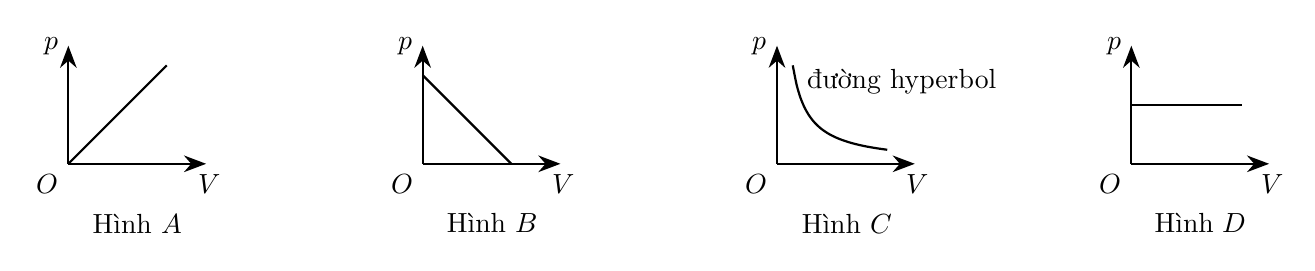
\begin{tikzpicture}[scale=0.5, thick, >={Stealth[length=8pt, width=6pt]}]
        \begin{scope}[shift={(0,0)}]
        \draw[->] (0,0) -- (3.5,0) node[below]{${V}$};
        \draw[->] (0,0) -- (0,3) node[left]{${p}$};
        \draw[thick] (0,0) -- (2.5,2.5);
        \node[below left] at (0,0) {${O}$};
        \node[below] at (1.75,-1) {Hình $A$};
        \end{scope}

        \begin{scope}[shift={(9,0)}]
        \draw[->] (0,0) -- (3.5,0) node[below]{${V}$};
        \draw[->] (0,0) -- (0,3) node[left]{${p}$};
        \draw[thick] (0,2.25) -- (2.25,0);
        \node[below left] at (0,0) {${O}$};
        \node[below] at (1.75,-1) {Hình $B$};
        \end{scope}

        \begin{scope}[shift={(18,0)}]
        \draw[->] (0,0) -- (3.5,0) node[below]{${V}$};
        \draw[->] (0,0) -- (0,3) node[left]{${p}$};
        \draw[thick, smooth, domain=0.4:2.8] plot (\x, {1/\x});
        \node[below left] at (0,0) {${O}$};
        \node[above right] at (0.5,1.5) {đường hyperbol};
        \node[below] at (1.75,-1) {Hình $C$};
        \end{scope}

        \begin{scope}[shift={(27,0)}]
        \draw[->] (0,0) -- (3.5,0) node[below]{${V}$};
        \draw[->] (0,0) -- (0,3) node[left]{${p}$};
        \draw[thick] (0,1.5) -- (2.8,1.5);
        \node[below left] at (0,0) {${O}$};
        \node[below] at (1.75,-1) {Hình $D$};
        \end{scope}
    \end{tikzpicture}
    \end{center}
    \choice
    {Hình $A$}
    {Hình $B$}
    {\True Hình $C$}
    {Hình $D$}
    \loigiai{Trong hệ tọa độ ${p - V}$, đường đẳng nhiệt là đường cong Hyperbol.}
\end{ex}


% Câu 3
\begin{ex}
    Phát biểu nào sau đây về đường sức điện và đường sức từ là sai?
    \choice
    {\True Cả hai đều là đường cong khép kín}
    {Cả hai đều là đường tưởng tượng}
    {Chúng sẽ không giao nhau}
    {Cả hai đều sử dụng mật độ để chỉ độ mạnh yếu của trường}
    \loigiai{
Đường sức điện của điện trường tĩnh không khép kín.}
\end{ex}


% Câu 4
\begin{ex}
\immini[thm]{
        Một học sinh được cung cấp bộ thí nghiệm như hình bên dưới. Học sinh này có thể làm thí nghiệm kiểm chứng mối quan hệ giữa hai đại lượng của một khối khí xác định là
        \choice
        {\True thể tích và áp suất}
        {thể tích và nhiệt độ tuyệt đối}
        {thể tích và khối lượng}
        {áp suất và nhiệt độ tuyệt đối}
    }{
        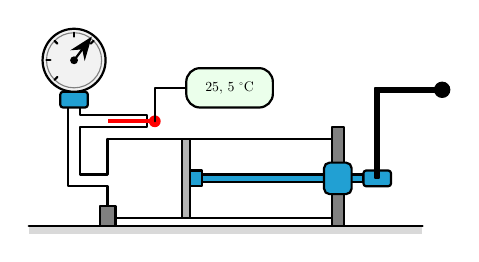
\begin{tikzpicture}[thick, line join=round, line cap=round, >=Stealth, transform shape, scale=0.5]
            % --- 1. MẶT ĐẤT ---
            \fill[gray!30] (0,-0.2) rectangle (10,0);
            \draw[thick] (0,0) -- (10,0);

            % --- 2. XI-LANH (CYLINDER) ---
            % Thân xi-lanh
            \draw[black, thick] (2, 1) -- (2,0.2) -- (7.9,0.2) (2,2.2) -- (7.9,2.2);
            \draw[fill=gray, thick] (7.7,0) rectangle (8.0,2.5); % Chặn đầu phải
            \draw[fill=gray, thick] (1.8,0) rectangle (2.2,0.5); % Chân đế trái
            % \node[above] at (5, 2.2) {Cylinder};

            % Piston bên trong
            \draw[thick, fill = gray!60] (3.9,0.2) rectangle (4.1,2.2);
            % \node[left] at (3.9,1.5) {piston};
            
            % Cần Piston (Rod)
            \draw[fill=cyan!85!black, draw=black] (4.1, 1.0) rectangle (4.4, 1.4); % Khớp nối piston
            \draw[fill=cyan!85!black, draw=black] (4.4, 1.1) rectangle (8.5, 1.3); % Thanh truyền
            \draw[fill=cyan!85!black, draw=black, rounded corners=2pt] (7.5, 0.8) rectangle (8.2, 1.6); % Khớp chặn đầu
            \draw[fill=cyan!85!black, draw=black, rounded corners=1pt] (8.5, 1.0) rectangle (9.2, 1.4); % Đầu nối tay quay

            % --- 3. TAY QUAY (CRANK) ---
            \draw[fill=black] (8.8, 1.2) -- (8.8, 3.5) -- (10.5, 3.5) -- (10.5,3.4) -- (8.9, 3.4) -- (8.9,1.2) -- cycle;
            \draw[fill=black] (10.5, 3.45) circle (0.18);
            % \node[above] at (9.6, 3.5) {Tay quay};

            % --- 4. HỆ THỐNG ỐNG DẪN VÀ ÁP KẾ ---
            % Ống dẫn khí (blue)
            \draw[black, thick] (2, 1) -- (1, 1) -- (1, 3);
            \draw[black, thick] (2, 2.2) -- (2, 1.3) -- (1.3, 1.3) -- (1.3, 2.5) -- (3, 2.5) -- (3, 2.8) -- (1.3, 2.8) -- (1.3, 3); % Nhánh ngang
            
            % Đầu nối Áp kế
            \fill[cyan!85!black, draw=black, rounded corners=1pt] (0.8, 3) rectangle (1.5, 3.4);
            
            % Mặt Áp kế (Pressure Gauge)
            \draw[fill=gray!10, thick] (1.15, 4.2) circle (0.8);
            \draw[gray, thin] (1.15, 4.2) circle (0.7);
            % \node[right] at (1.95, 4.2) {Áp kế};
            
            % Kim áp kế
            \fill[black] (1.15, 4.2) circle (0.1);
            \draw[-{Stealth[length=3mm]}, thick] (1.15, 4.2) -- (1.6, 4.8);
            \foreach \a in {45, 90, 135, 180, 225}
                \draw (1.15, 4.2) ++(\a:0.6) -- ++(\a:0.1);

            % --- 5. CẢM BIẾN NHIỆT ĐỘ ---
            % Đầu dò nhiệt (Màu đỏ)
            \fill[fill=red] (2, 2.6) rectangle (3.2, 2.7);
            \fill[red] (3.2, 2.65) circle (0.15);
            
            % Dây dẫn
            \draw[black, thick] (3.2, 2.65) -- (3.2, 3.5) -- (4, 3.5);
            
            % Màn hình hiển thị
            \draw[fill=green!8, thick, rounded corners=5pt] (4, 3) rectangle (6.2, 4);
            \node at (5.1, 3.5) {\textifsym{25}$,$ \textifsym{5} $^\circ \mathrm{C}$};
            % \node[above] at (5.1, 4) {Cảm biến nhiệt độ};

        \end{tikzpicture}
    }
    \loigiai{Bộ thí nghiệm trên kiểm chứng định luật Boyle trong điều kiện nhiệt độ khối khí không đổi. Kiểm chứng được mối quan hệ giữa hai đại lượng áp suất và thể tích của khối khí.}
\end{ex}


% Câu 5
\begin{ex}
    Trong giờ thực hành Vật lí, một học sinh thực hiện thí nghiệm khảo sát sự biến thiên nội năng của một khối khí xác định chứa trong cylinder kín. Bạn tiến hành nhúng phần thân chứa khí vào nước đá lạnh và dùng tay nhấn mạnh piston để nén nhanh khối khí. Theo quy ước về dấu của Nguyên lí I nhiệt động lực học thì
    \choice
    {${A < 0; Q > 0}$}
    {\True ${A > 0; Q < 0}$}
    {${A > 0; Q > 0}$}
    {${A < 0; Q < 0}$}
    \loigiai{Trong trường hợp này, khối khí trong cylinder đang nhận công từ học sinh (${A > 0}$) và tỏa nhiệt khi tiếp xúc với nước lạnh (${Q < 0}$).}
\end{ex}


% Câu 6
\begin{ex}
    Ở các vùng núi cao, người dân thường thấy những ngày băng tuyết tan chảy (tan băng) trời lạnh buốt hơn hẳn so với những ngày tuyết đang rơi. Nguyên nhân chủ yếu của hiện tượng này là do quá trình băng tan
    \choice
    {tỏa nhiệt lượng ra môi trường xung quanh khiến nhiệt độ không khí giảm}
    {\True thu nhiệt lượng từ môi trường xung quanh khiến nhiệt độ không khí giảm}
    {làm giảm độ ẩm của không khí xung quanh}
    {cản trở sự đối lưu của dòng khí nóng}
    \loigiai{Quá trình tuyết tan (băng tan) là quá trình nóng chảy. Khi này vật sẽ thu nhiệt lượng từ bên ngoài và khiến cho nhiệt độ không khí giảm.}
\end{ex}


% Câu 7
\begin{ex}
    Trong công nghệ in 3D, vật liệu in được gia nhiệt để chuyển sang thể lỏng và đùn qua đầu phun để tạo thành từng lớp. Ngay sau khi ra khỏi đầu phun và tiếp xúc với không khí, vật liệu nhanh chóng chuyển từ thể lỏng sang thể rắn để định hình sản phẩm. Các quá trình chuyển thể nào liên quan trực tiếp đến công đoạn sản xuất mô hình theo công nghệ này?
    \choice
    {đông đặc và hóa hơi}
    {nóng chảy và ngưng tụ}
    {thăng hoa và ngưng kết}
    {\True nóng chảy và đông đặc}
    \loigiai{Vật liệu in được gia nhiệt chuyển từ thể rắn sang thể lỏng liên quan đến quá trình nóng chảy. Sau đó vật liệu chuyển từ thể lỏng sang thể rắn để định hình sản phẩm liên quan đến quá trình đông đặc.}
\end{ex}


% Câu 8
\begin{ex}
    Tại các bãi tái chế kim loại, người ta sử dụng cần cẩu trang bị nam châm điện lớn để nâng và di chuyển các khối sắt vụn. Nam châm điện này thực chất là một ống dây có lõi sắt. Trong quá trình vận hành, để nam châm có thể hút được một khối sắt nặng hơn, người điều khiển cần thực hiện thao tác nào sau đây?
    \choice
    {\True Tăng cường độ dòng điện chạy qua ống dây}
    {Đảo chiều dòng điện liên tục}
    {Giảm cường độ dòng điện chạy qua ống dây}
    {Giữ nguyên cường độ dòng điện và tăng thời gian hút}
    \loigiai{Để hút được khối sắt nặng hơn thì cần một lực từ lớn hơn. Vì vậy ta cần điều chỉnh sao cho cường độ dòng điện chạy trong ống dây tăng để tăng độ lớn lực từ.}
\end{ex}


% Câu 9 + 10
\begin{ex}
\sochc{2}{\immini[]{
    Một nhóm học sinh thực hiện mô hình cảm biến rung chấn đơn giản với các dụng cụ gồm: một nam châm thẳng mạnh được gắn bên trong lòng một cuộn dây, dây dẫn được kết nối với bộ xử lý và màn hình hiển thị. Khi có rung chấn, nam châm dao động làm xuất hiện dòng điện bên trong cuộn dây và tín hiệu sẽ được truyền đến màn hình hiển thị để báo động có sự rung chấn.
    }{
        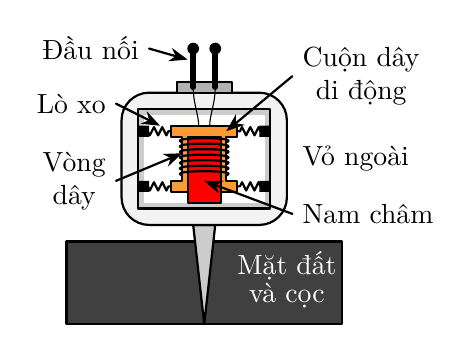
\begin{tikzpicture}[line join=round, thick, line cap=round, >=Stealth, scale=0.7]

            % --- 1. MẶT ĐẤT VÀ CỌC (SURFACE MATERIAL) ---
            \draw[fill=gray!50!black] (-2.5,-3) rectangle (2.5,-1.5);
            \node[white, align=center, font=\linespread{1}\selectfont] at (1.5,-2.2) {Mặt đất \\[-2pt] và cọc};
            % Cọc nhọn
            \draw[fill=gray!40] (0,-1.5) -- (0.2,-1.2) -- (-0.2,-1.2) -- cycle;
            \draw[fill=gray!40] (0,-3) -- (0.2,-1.2) -- (-0.2,-1.2) -- cycle;

            % --- 2. VỎ NGOÀI (GEOPHONE CASING) ---
            % Vỏ nhựa trắng
            \draw[fill=gray!10, rounded corners=10pt, thick] (-1.5,1.2) rectangle (1.5,-1.2);
            % Khung chì/kim loại bên trong
            \draw[fill=gray!40, thick] (-1.2,0.9) rectangle (1.2,-0.9);
            \fill[white] (-1.1,0.8) rectangle (1.1,-0.8);
            \node[right] at (1.6,0.0) {Vỏ ngoài};

            % --- 3. CUỘN DÂY DI ĐỘNG (MOVING WEIGHT / COIL) ---
            % Khung màu vàng (Moving weight)
            \draw[fill=orange!80, thick] (-0.6,0.6) -- (0.6,0.6) -- (0.6,0.4) -- (0.4,0.4) -- (0.4,-0.4) -- (0.6,-0.4) -- (0.6,-0.6) -- (-0.6,-0.6) -- (-0.6,-0.4) -- (-0.4,-0.4) -- (-0.4,0.4) -- (-0.6,0.4) -- cycle;
            \node[right, align=center, font=\linespread{1}\selectfont] at (1.6,1.5) {Cuộn dây \\ di động};
            \draw[->] (1.6,1.5) -- (0.4,0.5);
            
            % --- 4. NAM CHÂM (MAGNET) ---
            \draw[fill=red] (-0.3,-0.8) rectangle (0.3,0.4);
            \draw[<-] (0,-0.4) -- (1.6,-1) node[right] {Nam châm};

            % Các vòng dây (Coil)
            \foreach \y in {0.3, 0.2, 0.1, 0, -0.1, -0.2, -0.3} {
                \draw[thick] (-0.4, \y) .. controls (-0.7, \y+0.1) and (0.7, \y+0.1) .. (0.4, \y);
            }
            \draw[<-] (-0.4,0.1) -- (-1.6,-0.4) node[left, align=center, font=\linespread{1}\selectfont] {Vòng\\dây};

            % --- 5. LÒ XO (SPRINGS) ---
            \tikzset{spring/.style={decoration={zigzag, amplitude=1.5pt, segment length=3pt}, decorate}}
            
            % Vẽ 4 lò xo kết nối khung di động với vỏ
            \draw[spring] (-1.1, 0.5) -- (-0.6, 0.5);
            \draw[spring] (1.1, 0.5) -- (0.6, 0.5);
            \draw[spring] (-1.1, -0.5) -- (-0.6, -0.5);
            \draw[spring] (1.1, -0.5) -- (0.6, -0.5);
            
            % Các điểm chốt lò xo
            \foreach \x/\y in {-1.1/0.5, 1.1/0.5, -1.1/-0.5, 1.1/-0.5} \fill (\x,\y) rectangle ++(0.1,0.1) rectangle ++(-0.2,-0.2);
            \draw[<-] (-0.8,0.6) -- (-1.6,1.0) node[left, align=center] {Lò xo};

            % --- 6. CÁC ĐẦU NỐI (CONNECTORS) ---
            % Chân đế trên đầu
            \draw[fill=gray!60] (-0.5,1.2) rectangle (0.5,1.4);
            % Cọc nối
            \draw[line width=2pt] (-0.2,1.3) -- (-0.2,2.0) node[fill, circle, inner sep=1.5pt] {};
            \draw[line width=2pt] (0.2,1.3) -- (0.2,2.0) node[fill, circle, inner sep=1.5pt] {};
            \draw[<-] (-0.3,1.8) -- (-1.0,2.0)  node [left] {Đầu nối};

            % Dây nối từ Coil lên Connector
            \draw[thin] (-0.2,1.3) .. controls (-0.2,1) and (-0.1,0.8) .. (-0.1,0.6);
            \draw[thin] (0.2,1.3) .. controls (0.2,1) and (0.1,0.8) .. (0.1,0.6);

        \end{tikzpicture}
    }
}
    \begin{chc}
        Mô hình hoạt động dựa trên hiện tượng
        \choice
        {giao thoa sóng}
        {quang điện}
        {\True cảm ứng điện từ}
        {nhiễm điện do cọ xát}
        \loigiai{Khi nam châm chuyển động bên trong lòng cuộn dây, từ thông xuyên qua tiết diện của cuộn dây làm xuất hiện dòng điện cảm ứng (dựa trên hiện tượng cảm ứng điện từ). Dòng điện sẽ được truyền đến bộ xử lí và hiển thị trên màn hình.}
    \end{chc}

    \begin{chc}
        Nếu nhóm học sinh muốn tăng độ nhạy của cảm biến, biện pháp nào sau đây là phù hợp nhất?
        \choice
        {Dùng nam châm có từ trường yếu hơn}
        {Thay đổi cuộn dây có ít vòng hơn}
        {\True Tăng số vòng dây của cuộn dây}
        {Đặt cuộn dây cách xa nam châm hơn}
        \loigiai{Độ lớn suất điện động cảm ứng tỉ lệ với số vòng dây. Để tăng độ nhạy của cảm biến, nhóm học sinh nên tăng số vòng dây của cuộn dây.}
    \end{chc}
\end{ex}


% Câu 11
\begin{ex}
    Trong thí nghiệm Rutherford, khi bắn một chùm hạt ${\alpha}$ mang điện tích dương vào một lá vàng siêu mỏng và quan sát đường đi của chúng. Kết quả thực nghiệm cho thấy phần lớn các hạt ${\alpha}$ đi xuyên qua lá vàng mà không bị lệch hướng. Kết quả này là bằng chứng thực nghiệm quan trọng dẫn đến kết luận nào sau đây về cấu trúc nguyên tử?
    \choice
    {Tồn tại hạt nhân nguyên tử có cùng điện tích dương}
    {\True Nguyên tử chủ yếu là không gian rỗng}
    {Hạt nhân có kích thước rất nhỏ, chiếm gần như toàn bộ khối lượng nguyên tử}
    {Điện tích dương được phân bố đồng đều trong toàn bộ thể tích của nguyên tử}
    \loigiai{Kết quả thực nghiệm ``phần lớn các hạt ${\alpha}$ đi xuyên qua lá vàng mà không bị lệch hướng'' là bằng chứng thực nghiệm để đưa ra kết luận nguyên tử chủ yếu là không gian rỗng.}
\end{ex}


% Câu 12
\begin{ex}
    Gọi các tia phát ra từ các thiết bị: (1) Máy soi tiền giả, (2) Điều khiển từ xa TV, (3) Máy chụp CT (cắt lớp vi tính); tất cả đều là sóng điện từ, thứ tự tần số giảm dần là
    \choice
    {(1), (2), (3)}
    {(3), (2), (1)}
    {(2), (3), (1)}
    {\True (3), (1), (2)}
    \loigiai{Máy soi tiền giả là tia tử ngoại\\
Điều khiển từ xa TV là tia hồng ngoại\\Máy chụp CT (cắt lớp vi tính) là tia X\\Tần số tia X > tia tử ngoại > tia hồng ngoại ${\Rightarrow}$ (3), (1), (2).}
\end{ex}


% Câu 13
\begin{ex}
    Có thể gây ra vụ nổ nguyên tử bằng cách cho hai khối vật liệu phân hạch hạt nhân được làm giàu với độ tinh khiết rất cao chập vào nhau. Việc cho chập hai khối vật liệu phân hạch vào nhau nhằm mục đích
    \choice
    {tăng tổng khối lượng vật liệu phân hạch}
    {tăng tổng thể tích vật liệu phân hạch}
    {\True tăng hệ số nhân neutron của phản ứng phân hạch}
    {tăng công suất tỏa năng lượng phân hạch}
    \loigiai{Khi ${k > 1}$ thì phản ứng phân hạch dây chuyền có thể gây nên bùng nổ.}
\end{ex}


% Câu 14 + 15
\begin{ex}
\sochc{2}{\immini[]{
    Một học sinh dùng bếp điện có công suất ${750 \, \mathrm{W}}$ để đun nóng ${1{,}8 \, \mathrm{kg}}$ chất $X$ ở thể rắn và vẽ được đồ thị biểu diễn sự thay đổi nhiệt độ của chất $X$ theo thời gian như hình bên. Bỏ qua sự trao đổi nhiệt với môi trường bên ngoài.
    }{
        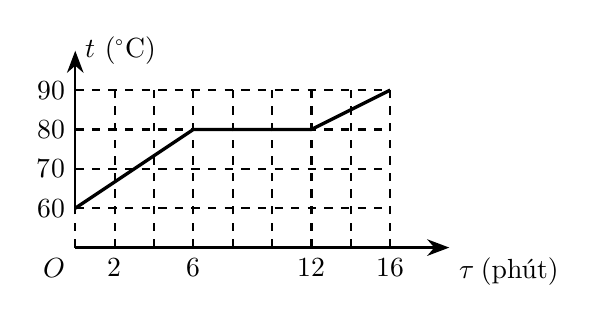
\begin{tikzpicture}[scale=0.5, thick, >={Stealth[length=8pt, width=6pt]}]
            \draw[dashed] (0,0) grid (8,4);
            \draw[->] (0,0) -- (9.5,0) node[below right] {${\tau}$ (phút)};
            \draw[->] (0,1) -- (0,5) node[right] {${t}$ (${^\circ\mathrm{C}}$)};
            \foreach \x in {2,6,12,16} \node[below] at (\x/2,0) {${\x}$};
            \foreach \y [count=\i] in {60,70,80,90} \node[left] at (0,\i) {${\y}$};
            \draw[very thick] (0,1) -- (3,3) -- (6,3) -- (8,4);
            \node[below left] at (0,0) {${O}$};
        \end{tikzpicture}
        }}
    \begin{chc}
        Nhiệt độ nóng chảy của chất $X$ là
        \choice
        {${60 \, ^\circ\mathrm{C}}$}
        {${-70 \, ^\circ\mathrm{C}}$}
        {\True ${80 \, ^\circ\mathrm{C}}$}
        {${90 \, ^\circ\mathrm{C}}$}
        \loigiai{Dựa vào đồ thị ta xác định được nhiệt độ nóng chảy của chất $X$ là ${80 \, ^\circ\mathrm{C}}$.}
    \end{chc}

    \begin{chc}
        Nhiệt nóng chảy riêng của chất $X$ xấp xỉ bằng
        \choice
        {${150000 \, \mathrm{kJ/kg}}$}
        {${150 \, \mathrm{MJ/kg}}$}
        {\True ${150 \, \mathrm{kJ/kg}}$}
        {${150 \, \mathrm{J/kg}}$}
        \loigiai{
        ${Q = Pt = 750 \cdot \left(12 - 6\right) \cdot 60 = 270000 \, \mathrm{J}}$\\
        ${\lambda = \frac{Q}{m} = \frac{270000}{1{,}8} = 150 \cdot 10^3 \, \mathrm{J/kg} = 150 \, \mathrm{kJ/kg}}$.}
        \end{chc}
\end{ex}


% Câu 16
\begin{ex}
    Một hạt nhân trải qua hai phân rã ${\alpha}$ và một phân rã ${\beta^-}$ để trở thành một hạt nhân mới. So với số proton và neutron của hạt nhân ban đầu, hạt nhân mới
    \choice
    {ít hơn ${3}$ proton và nhiều hơn ${5}$ neutron}
    {\True ít hơn ${3}$ proton và ít hơn ${5}$ neutron}
    {nhiều hơn ${3}$ proton và nhiều hơn ${1}$ neutron}
    {nhiều hơn ${3}$ proton và ít hơn ${5}$ neutron}
    \loigiai{
    ${^A_Z X \to 2 ^4_2 \alpha + ^0_{-1} \beta^- + ^{A-8}_{Z-3} Y \Rightarrow}$ hạt nhân mới ít hơn ${3}$ proton và ${8 - 3 = 5}$ neutron.}
\end{ex}


% Câu 17
\begin{ex}
    Khi chụp cộng hưởng từ, để máy ghi nhận thông tin chính xác và tránh nguy hiểm phải bỏ trang sức kim loại khỏi cơ thể người bệnh. Giả sử có một vòng kim loại nằm trong máy sao cho mặt phẳng của vòng vuông góc với vector cảm ứng từ của từ trường do máy tạo ra khi chụp. Biết bán kính và điện trở của vòng này lần lượt là ${4{,}20 \, \mathrm{cm}}$ và ${0{,}01 \, \Omega}$. Nếu trong ${0{,}40 \, \mathrm{s}}$, độ lớn cảm ứng từ của từ trường do máy tạo ra giảm đều từ ${1{,}50 \, \mathrm{T}}$ xuống ${0{,}20 \, \mathrm{T}}$ thì cường độ dòng điện trong vòng kim loại này có độ lớn bằng
    \choice
    {\True ${1{,}8 \, \mathrm{A}}$}
    {${1{,}9 \, \mathrm{A}}$}
    {${1{,}5 \, \mathrm{A}}$}
    {${3{,}8 \, \mathrm{A}}$}
    \loigiai{
        ${e = \left| \frac{\Delta \Phi}{\Delta t} \right| = \left| \frac{\Delta B \cdot S}{\Delta t} \right| = \left| \frac{\Delta B \cdot \pi r^2}{\Delta t} \right| = \frac{\left(1{,}5 - 0{,}2\right) \cdot \pi \cdot 0{,}042^2}{0{,}4} \approx 0{,}018 \, \mathrm{V}}$\\
        ${i = \frac{e}{R} = \frac{0{,}018}{0{,}01} = 1{,}8 \, \mathrm{A}}$.}
\end{ex}


% Câu 18
\begin{ex}
    Một lốp ô tô có thể tích không đổi ${30}$ lít. Ở địa điểm A, khí trong lốp ở nhiệt độ ${-3 \, ^\circ\mathrm{C}}$ và áp suất ${2{,}7 \cdot 10^5 \, \mathrm{Pa}}$. Khi di chuyển tới địa điểm B, khí trong lốp có nhiệt độ ${-23 \, ^\circ\mathrm{C}}$. Tại đây, lốp được bơm thêm không khí ở ${-23 \, ^\circ\mathrm{C}}$ và áp suất ${10^5 \, \mathrm{Pa}}$ để áp suất lốp đạt ${2{,}7 \cdot 10^5 \, \mathrm{Pa}}$. Thể tích của lượng không khí được bơm thêm vào lốp là
    \choice
    {\True ${6}$ lít}
    {${3}$ lít}
    {${5}$ lít}
    {${4}$ lít}
    \loigiai{
${n_s = n_t + n_{bom} \xrightarrow{n = \frac{pV}{RT}} \frac{2{,}7 \cdot 10^5 \cdot 30}{-23 + 273} = \frac{2{,}7 \cdot 10^5 \cdot 30}{-3 + 273} + \frac{10^5 \cdot V}{-23 + 273} \Rightarrow V = 6 \, \mathrm{l}}$.}
\end{ex}


% Câu 1
\begin{ex}
    Một nhóm học sinh thực hiện thí nghiệm khảo sát quá trình làm nguội của nước. Nhóm sử dụng hai chậu giống nhau, mỗi chậu chứa ${2 \, \mathrm{kg}}$ nước nóng có nhiệt độ ban đầu là ${50 \, ^\circ\mathrm{C}}$. Thí nghiệm được tiến hành trong phòng có nhiệt độ ${25 \, ^\circ\mathrm{C}}$. Chậu 1 để nguội tự nhiên và chậu 2 dùng quạt thổi gió qua mặt thoáng. Trong quá trình đo, học sinh liên tục khuấy nhẹ nước và phòng lặng gió. Kết quả đo nhiệt độ nước sau mỗi phút được ghi lại bằng bảng bên dưới:
    \begin{center}
    \begin{tabular}{|c|c|c|c|c|c|}
    \hline
    Thời gian (phút) & 1 & 2 & 3 & 4 & 5 \\ \hline
    Nhiệt độ khi không có gió (${^\circ\mathrm{C}}$) & 46,0 & 43,5 & 41,5 & 40,0 & 39,0 \\ \hline
    Nhiệt độ khi có gió (${^\circ\mathrm{C}}$) & 43,0 & 39,0 & 36,0 & 34,0 & 32,3 \\
    \hline
    \end{tabular}
    \end{center}
    \choiceTF[1]
    {\True Trong thí nghiệm này, nước trong chậu đang tỏa nhiệt ra môi trường xung quanh}
    {Nhiệt độ của nước ở chậu 2 giảm nhanh hơn so với chậu 1 là do quá trình bay hơi trên mặt thoáng ở chậu 2 diễn ra chậm hơn}
    {\True Thao tác khuấy nhẹ nước liên tục giúp nhiệt độ tại mọi điểm trở nên đồng đều, đảm bảo số liệu đo được chính xác hơn}
    {Tại thời điểm phút thứ 5, khối lượng nước trong cả 2 chậu là như nhau}
    \loigiai{
        \begin{itemchoice}
        \itemch Do nhiệt độ của nước cao hơn nhiệt độ phòng nên nước sẽ tỏa nhiệt ra môi trường xung quanh theo nguyên lí truyền nhiệt.
        \itemch Nhiệt độ của nước ở chậu 2 giảm nhanh hơn so với chậu 1 là do quá trình bay hơi trên mặt thoáng ở chậu 2 diễn ra nhanh hơn vì ảnh hưởng bởi tốc độ gió.
        \itemch 
        \itemch Tại phút thứ 5, khối lượng nước trong chậu 2 sẽ bé hơn trong chậu 1 vì lượng nước đã hóa hơi trong chậu 2 sẽ nhiều hơn so với chậu 1.
        \end{itemchoice}
    }
\end{ex}


% Câu 2
\begin{ex}
\immini[thm]{
    Loa điện động hoạt động dựa trên tác dụng từ giữa nam châm vĩnh cửu và cuộn dây dẫn. Cấu tạo chính gồm một cuộn dây nhẹ gắn chặt với màng loa, được đặt trong khe hở từ của nam châm vĩnh cửu, nơi có các đường sức từ hướng xuyên tâm. Xét một mẫu loa có ống dây gồm ${N = 100}$ vòng, quấn sát nhau tạo thành ống dây có chiều dài ống ${L = 2 \, \mathrm{cm}}$.
    }{
        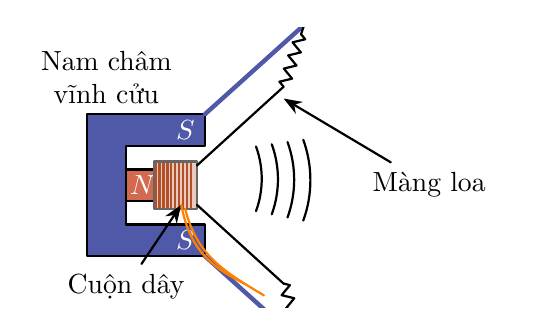
\begin{tikzpicture}[thick, line join=round, line cap=round, >=Stealth, scale=0.5, rotate=0]
            \clip (-1.5,-3.1) rectangle (11,4);
            % --- Định nghĩa màu sắc ---
            \definecolor{magRed}{RGB}{210, 106, 79}
            \definecolor{magBlue}{RGB}{80, 89, 168}
            \definecolor{coilOrange}{RGB}{180, 80, 40}
            \definecolor{labelPurple}{RGB}{140, 60, 140}

            % --- 1. NAM CHÂM VĨNH CỬU (Mặt cắt chữ E) ---
            % Phần lưng và hai nhánh chữ S
            \fill[magBlue] (0, -1.8) rectangle (1, 1.8);
            \fill[magBlue] (0.8, 1) rectangle (3, 1.8);
            \fill[magBlue] (0.8, -1.8) rectangle (3, -1);
            
            % Phần cực N ở giữa
            \draw[fill=magRed] (1, -0.4) rectangle (2, 0.4);
            
            % Viền cho nam châm
            \draw[thick, black] (0,-1.8) -- (0,1.8) -- (3,1.8) -- (3,1) -- (1,1) -- (1,0.4) -- (2,0.4) -- (2,-0.4) -- (1,-0.4) -- (1,-1) -- (3,-1) -- (3,-1.8) -- cycle;

            % Nhãn cực N và S
            \node[white] at (1.4, 0) {$N$};
            \node[white] at (2.5, 1.4) {$S$};
            \node[white] at (2.5, -1.4) {$S$};

            % --- 2. CUỘN DÂY (VOICE COIL) ---
            % Vẽ các vòng dây bao quanh cực N
            \begin{scope}
                \clip (1.7, -0.6) rectangle (2.8, 0.6);
                \fill[coilOrange!30] (1.7, -0.6) rectangle (2.8, 0.6);
                \foreach \x in {1.75, 1.85, ..., 2.75} {
                    \draw[coilOrange, thick] (\x, -0.6) -- (\x, 0.6);
                }
            \end{scope}
            \draw[thick, black!60] (1.7, -0.6) rectangle (2.8, 0.6);

            % --- 3. MÀNG LOA (DIAPHRAGM) ---
            % Nhánh trên
            \draw[ultra thick, magBlue] (3, 1.8) -- (6, 4.5);
            \draw[thick] (2.8, 0.5) -- (5, 2.5);
            \draw[decorate, decoration={zigzag, segment length=5pt, amplitude=2pt}] (5, 2.5) -- (5.5, 4);

            % Nhánh dưới
            \draw[ultra thick, magBlue] (3, -1.8) -- (6, -4.5);
            \draw[thick] (2.8, -0.5) -- (5, -2.5);
            \draw[decorate, decoration={zigzag, segment length=5pt, amplitude=2pt}] (5, -2.5) -- (5.5, -4);

            % --- 4. SÓNG ÂM ---
            \foreach \r in {0.8, 1.2, 1.6, 2.0} {
                \draw[thick] (3.5 + \r, -0.5-\r*0.2) arc (-20:20:2 + \r*0.5);
            }

            % --- 5. CHÚ THÍCH (LABELS) ---
            
            % Nam châm vĩnh cửu
            \node[above, align=center, font=\linespread{1}\selectfont] (L1) at (0.5, 1.8) {Nam châm\\vĩnh cửu};
            
            % Màng loa
            \node[right] (L2) at (7, 0) {Màng loa};
            \draw[->] (L2) -- (5, 2.2);

            % Cuộn dây
            \node[below] (L3) at (1.0, -2.0) {Cuộn dây};
            \draw[->] (L3) -- (2.4, -0.5);

            % Dây nối lò xo (màu cam nhạt trong hình)
            \draw[orange, thick] (2.4, -0.5) .. controls (2.6, -1.5) and (3, -2) .. (4, -2.5);
            \draw[orange, thick] (2.5, -0.6) .. controls (2.8, -1.8) and (3.5, -2.2) .. (4.5, -2.8);

        \end{tikzpicture}
    }
    \choiceTF[1]
    {\True Khi có dòng điện xoay chiều đi qua, cuộn dây đóng vai trò như một nam châm điện, tương tác với nam châm vĩnh cửu và khiến cho màng loa dao động để tạo ra âm thanh}
    {Nguyên lí hoạt động của loa điện động là hiện tượng cảm ứng điện từ}
    {Để loa hoạt động ổn định và phát ra âm thanh liên tục, ta có thể nối hai đầu cuộn dây với nguồn điện một chiều có cường độ dòng điện không đổi}
    {\True Biết độ lớn cảm ứng từ trong cuộn dây được tính bằng công thức ${4\pi \cdot 10^{-7} \cdot \frac{NI}{L}}$. Giả sử dòng điện trong cuộn dây tại một thời điểm có cường độ ${2 \, \mathrm{A}}$, cảm ứng từ do chính cuộn dây sinh ra trong lòng nó có độ lớn khoảng ${12{,}6 \, \mathrm{mT}}$}
    \loigiai{
        \begin{itemchoice}
        \itemch Khi có dòng điện xoay chiều đi qua, cuộn dây hoạt động như một nam châm điện và nó sẽ tương tác với nam châm vĩnh cửu gắn trong loa, từ đó khiến màng loa dao động và tạo ra âm thanh.
        \itemch Loa điện động hoạt động dựa vào sự tương tác từ giữa nam châm vĩnh cửu và cuộn dây khi có dòng điện xoay chiều đi qua.
        \itemch Trong trường hợp sử dụng dòng điện một chiều, cực của nam châm điện không đổi chiều và sẽ không làm cho màng loa dao động nhờ quá trình hút - đẩy khi tương tác với nam châm vĩnh cửu.
        \itemch ${B = 4\pi \cdot 10^{-7} \cdot \frac{NI}{L} = 4\pi \cdot 10^{-7} \cdot \frac{100 \cdot 2}{0{,}02} \approx 12{,}6 \cdot 10^{-3} \, \mathrm{T} = 12{,}6 \, \mathrm{mT}}$.
        \end{itemchoice}
    }
\end{ex}


% Câu 3
\begin{ex}
\immini[thm]{
    Một nhóm học sinh thiết lập sơ đồ thí nghiệm như hình bên để ``nghiên cứu mối quan hệ giữa áp suất và thể tích của một khối khí nhất định ở nhiệt độ không đổi''.
    \begin{itemize}
        \item Trong hình, thiết bị thí nghiệm $A$ là \_\_ (1) \_\_.
        \item Nhóm học sinh đã đo hai bộ dữ liệu $(p, V)$ khác nhau trong hai thí nghiệm khác nhau và thấy rằng tích của $p$ và $V$ trong hai bộ dữ liệu khác nhau đáng kể, lí do có thể là \_\_ (2) \_\_.
        \item Để giữ nhiệt độ của khí trong xilanh không đổi, biện pháp được thực hiện trong thí nghiệm là: \_\_ (3) \_\_.
        \item Ban đầu khí trong xilanh có thể tích ${10 \, \mathrm{cm^3}}$ và áp suất bằng áp suất khí quyển bên ngoài là ${p_0}$. Trong quá trình thí nghiệm, thể tích khí trong xilanh thay đổi từ ${4 \, \mathrm{cm^3}}$ đến ${20 \, \mathrm{cm^3}}$. Chênh lệch áp suất khí bên trong xilanh và bên ngoài lớn nhất là \_\_ (4) \_\_.
    \end{itemize}
    }{ 
        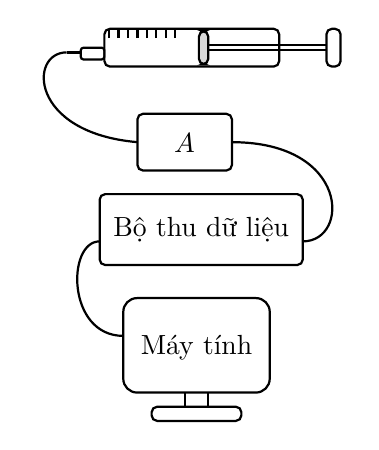
\begin{tikzpicture}[thick, rounded corners=2pt, scale = 0.6]
            % --- Vẽ Thiết bị A (Cảm biến áp suất) ---
            \begin{scope}[shift={(1.5,-2)}]
                \draw (0,0) rectangle (2,1.2);
                \node at (1,0.6) {$A$};
            \end{scope}

            % --- Vẽ Xi-lanh ---
            \begin{scope}[shift={(-2,0)}]
                % Thân xi-lanh
                \draw (2.8,0.2) rectangle (6.5,1);
                % Đầu nối giữa A và Xi-lanh
                \draw (2,0.5) -- (2.3,0.5);
                \draw[rounded corners=1pt] (2.3,0.35) rectangle (2.8,0.6);
                % Vạch chia độ
                \foreach \x in {0,0.2,...,1.4}
                    \draw (2.9+\x, 0.8) -- (2.9+\x, 1);
                
                % --- Vẽ Pít-tông ---
                % Đĩa pít-tông bên trong
                \fill[gray!30] (4.8,0.25) rectangle (5,0.95);
                \draw (4.8,0.25) rectangle (5,0.95);
                % Cần pít-tông
                \draw (5,0.55) -- (7.5,0.55);
                \draw (5,0.65) -- (7.5,0.65);
                % Tay cầm pít-tông
                \draw (7.5,0.2) rectangle (7.8,1);
            \end{scope}

            % --- Vẽ Bộ thu dữ liệu ---
            \begin{scope}[shift={(0.5,-1.5)}]
                \draw (0.2,-2.5) rectangle (4.5,-1);
                \node at (2.35,-1.75) {Bộ thu dữ liệu};
            \end{scope}

            % --- Vẽ Máy tính ---
            \begin{scope}[shift={(-4,-4)}]
                % Màn hình
                \draw[rounded corners=5pt] (5.2,-2.7) rectangle (8.3,-0.7);
                \node at (6.75,-1.75) {Máy tính};
                % Đế màn hình
                \draw (6.5,-2.7) -- (6.5,-3.0);
                \draw (7,-2.7) -- (7,-3.0);
                \draw (5.8,-3.3) rectangle (7.7,-3.0);
            \end{scope}

            % --- Vẽ dây kết nối ---
            % Bơm tiêm -> A (trung điểm cạnh trái của A)
            \draw[] (0,0.5) .. controls (-0.8,0.5) and (-0.8,-1.2) .. (1.5, -1.4);
            % Cạnh phải A -> cạnh phải bộ thu dữ liệu
            \draw[] (3.5,-1.4) .. controls (6.0,-1.4) and (6.0,-3.5) .. (5.0,-3.5);
            % Cạnh trái bộ thu -> máy tính
            \draw[] (0.7,-3.5) .. controls (0,-3.5) and (0,-5.5) .. (1.2,-5.5);
        \end{tikzpicture}
    }
    \choiceTF[1]
    {(1): cảm biến nhiệt độ}
    {\True (2): nhiệt độ môi trường khác nhau và khối lượng khí trong xilanh khác nhau}
    {(3): tay giữ chắc phần thân xilanh và đẩy kéo piston dứt khoát}
    {\True (4): ${1{,}5 p_0}$}
    \loigiai{
        \begin{itemchoice}
        \itemch Cảm biến áp suất (áp kế).
        \itemch ${pV = \frac{m}{M} RT \Rightarrow}$ do $T$ khác nhau hoặc $m$ khác nhau dẫn đến $pV$ khác nhau.
        \itemch Làm như vậy nhiệt độ sẽ thay đổi.
        \itemch ${pV = const \Rightarrow p_0 \cdot 10 = p_1 \cdot 4 = p_2 \cdot 20 \Rightarrow \left\{\begin{aligned} & p_1 = 2{,}5 p_0 \\ & p_2 = 0{,}5 p_0 \end{aligned}\right. \Rightarrow \Delta p_{max} = p_1 - p_0 = 1{,}5 p_0}$.
        \end{itemchoice}
    }
\end{ex}


% Câu 4
\begin{ex}
    Tuổi của một chiếc thuyền cổ có thể được xác định bằng cách so sánh sự phân rã phóng xạ của ${^{14}_6 \mathrm{C}}$ từ gỗ tươi với gỗ lấy từ chiếc thuyền cổ. Một mẫu gỗ gồm ${3 \cdot 10^{23}}$ nguyên tử carbon được lấy ra từ một khối gỗ tươi để nghiên cứu. Trong gỗ tươi, cứ ${10^{12}}$ nguyên tử carbon thì có ${1}$ nguyên tử là đồng vị phóng xạ ${^{14}_6 \mathrm{C}}$ có hằng số phóng xạ là ${3,84 \cdot 10^{-12} \, \mathrm{s^{-1}}}$. Lấy ${1}$ năm có ${365}$ ngày. Người ta lấy từ chiếc thuyền cổ này một mẫu gỗ cổ (bằng khối lượng của mẫu gỗ tươi) và xác định được độ phóng xạ của các đồng vị phóng xạ ${^{14}_6 \mathrm{C}}$ trong mẫu này là ${0{,}65 \, \mathrm{Bq}}$.
    \choiceTF[1]
    {\True Chu kì bán rã của ${^{14}_6 \mathrm{C}}$ xấp xỉ bằng ${5724}$ năm}
    {\True Số nguyên tử ${^{14}_6 \mathrm{C}}$ có trong mẫu gỗ tươi trên là ${3 \cdot 10^{11}}$}
    {Độ phóng xạ của ${^{14}_6 \mathrm{C}}$ có trong mẫu gỗ tươi trên xấp xỉ bằng ${2 \, \mathrm{Bq}}$}
    {Tuổi của chiếc thuyền này xấp xỉ bằng ${2700}$ năm}
    \loigiai{
        \begin{itemchoice}
        \itemch Chu kì bán rã của ${^{14}_6 \mathrm{C}}$ bằng: ${T = \frac{\ln 2}{\lambda} = \frac{\ln 2}{3{,}84 \cdot 10^{-12}} \approx 1{,}8 \cdot 10^{11} \, \mathrm{s} \approx 5724}$ năm.
        \itemch ${N_0 = \frac{3 \cdot 10^{23}}{10^{12}} = 3 \cdot 10^{11}}$.
        \itemch ${H_0 = \lambda N_0 = 3{,}84 \cdot 10^{-12} \cdot 3 \cdot 10^{11} = 1{,}152 \, \mathrm{Bq}}$.
        \itemch ${H = H_0 \cdot 2^{\frac{-t}{T}} \Rightarrow 0{,}65 = 1{,}152 \cdot 2^{\frac{-t}{5724}} \Rightarrow t \approx 4726}$ năm.
        \end{itemchoice}
    }
\end{ex}


% Câu 1 + 2
\begin{ex}
    \sochc{2}{Trong kĩ thuật chụp PET/CT hiện đại để tầm soát ung thư, các bác sĩ sử dụng đồng vị phóng xạ Fluorine ${^{18} \mathrm{F}}$ tích hợp với phân tử đường. khi tiêm vào cơ thể, tế bào ung thư sẽ hấp thụ mạnh hợp chất này, từ đó phát sáng trên màn hình máy quét. Biết đồng vị ${^{18} \mathrm{F}}$ có chu kì bán rã là ${110}$ phút. Tại một trung tâm y học hạt nhân một liều thuốc phóng xạ vừa được điều chế xong có độ phóng xạ ban đầu là ${H_0 = 250 \, \mathrm{MBq}}$.
    }
    \begin{chc}
        Sau khoảng thời gian ${5}$ tiếng kể từ lúc điều chế, do sự chậm trễ trong khâu vận chuyển, liều thuốc mới đến được phòng tiêm. Lúc này, độ phóng xạ của liều thuốc còn lại là bao nhiêu $\mathrm{MBq}$? (Làm tròn kết quả đến chữ số hàng phần mười)
        \shortans{37,8}
        \loigiai{
        ${H = H_0 \cdot 2^{\frac{-t}{T}} = 250 \cdot 2^{\frac{-300}{110}} \approx 37{,}8 \, \mathrm{MBq}}$.}
    \end{chc}

    \begin{chc}
        Theo quy chuẩn an toàn bức xạ của bệnh viện (giả sử bỏ qua sự đào thải sinh học), bệnh nhân sau khi chụp xong phải ở lại phòng cách ly và chỉ được ra về khi độ phóng xạ trong cơ thể giảm xuống còn bằng ${3{,}125\%}$ so với độ phóng xạ lúc vừa tiêm. Nếu bệnh nhân được tiêm ngay khi thuốc có độ phóng xạ ${H_0}$ nói trên thì thời gian cách ly tối thiểu bao nhiêu phút?
        \shortans{550}
        \loigiai{
        ${H = H_0 \cdot 2^{\frac{-t}{T}} \Rightarrow \frac{3{,}125}{100} = 2^{\frac{-t}{110}} \Rightarrow t = 550}$ phút.}
    \end{chc}
\end{ex}


% Câu 3 + 4
\begin{ex}
    \sochc{2}{\immini[]{
    Một khung dây dẫn phẳng có diện tích ${S = 0{,}005 \, \mathrm{m^2}}$ gồm ${N = 250}$ vòng dây, đang quay đều với tốc độ góc ${\omega = 50\pi \, \mathrm{rad/s}}$ quanh một trục đối xứng nằm trong mặt phẳng khung dây, trong một từ trường đều với cảm ứng từ ${B = 0{,}5 \, \mathrm{T}}$. Biết trục quay vuông góc với các đường sức của trường từ. Hai đầu khung dây được nối vào hai vành khuyên, sau đó được dẫn ra ngoài qua hai thanh quét (1) và (2) như mô tả trên hình vẽ. Nối hai đầu khung dây với điện trở ${R = 15\Omega}$ tạo thành một mạch kín.
    }{
    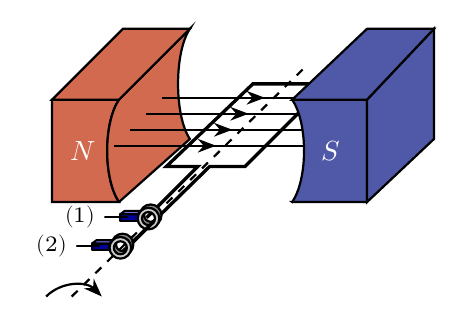
\begin{tikzpicture}[thick, >=Stealth, yscale=-1, scale = 0.1]
        \definecolor{magRed}{RGB}{210, 106, 79}
        \definecolor{magBlue}{RGB}{80, 89, 168}
        % N
        \draw[fill = magRed] (12.5, 32.0) -- (21.0, 32.0) .. controls (19, 29.0) and (19, 22.0) .. (21.0, 19.0) -- (12.5, 19.0) -- cycle;
        \node at ($(12.5,32.0)!0.5!(20.0,19.0)$)[white] {$N$};
        \draw[fill = magRed] (21.0, 32.0) -- (21.0, 32.0) .. controls (19, 29.0) and (19, 22.0) .. (21.0, 19.0) -- (30.0, 10.0) .. controls (28.0, 13.0) and (28.0, 21.0) .. (30.0, 24.0) -- (21.0, 32.0);
        \draw[fill = magRed] (12.5, 19.0) -- (21.0, 19.0) -- (30.0, 10.0) -- (21.5, 10.0) -- cycle;

        % Trục
        \draw[dashed] (15.0, 44.0) -- (44.5, 15.0);

        % B
        \foreach \t in {0.35, 0.42, ...,0.6} {
            \path 
            ($(15, 35)!\t!(44.5, 6) + (-5,0)$) coordinate (A)
            ($(15, 35)!\t!(44.5, 6) + (20,0)$) coordinate (B);

            \draw (A) -- (B);

            \draw[->] ($(A)!0.48!(B)$) -- ($(A)!0.52!(B)$);
        }

        % Khung dây
        \draw[very thick] (20.75, 39.0) -- (32.5, 27.5) -- (37.0, 27.5) -- (47.5, 17.0) -- (38.0, 17.0) -- (27.0, 27.5) -- (31.0, 27.5) -- (24.5, 34.0);

        % S
        \draw[fill = magBlue] (43.0, 32.0) -- (52.5, 32.0) -- (52.5, 19.0) -- (43.0, 19.0) .. controls (45, 22.0) and (45, 29.0) .. cycle;
        \node at ($(43.0,32.0)!0.5!(52.5,19.0)$)[white] {$S$};
        \draw[fill = magBlue] (52.5, 32.0) -- (61.0, 24.0) -- (61.0, 10.0)  -- (52.5, 19.0) -- cycle;
        \draw[fill = magBlue] (43.0, 19.0) -- (52.5, 19.0) -- (61.0, 10.0)  -- (52.5, 10.0) -- cycle;

        \begin{scope}[line join=round, line cap=round, scale=2.75, yscale = -1, thick, shift = {(7.7, -13.75)}]
        % --- 4. Vẽ chổi quét (Khối màu xanh) ---
        % Mặt bên của chổi
        \filldraw[fill=blue!60!black, draw=black] (-1.3, -0.1) -- (-0.5, -0.1) -- (-0.5, 0.2) -- (-1.3, 0.2) -- cycle;
        % Mặt trên của chổi
        \filldraw[fill=blue!50, draw=black] (-1.3, 0.2) -- (-0.5, 0.2) -- (-0.3, 0.35) -- (-1.1, 0.35) -- cycle;

        % --- 5. Dây dẫn và nhãn (2) ---
        \draw (-1., 0.07) -- (-2, 0.07);
        \fill (-2, 0.07) circle (1pt);
        \node[left, font=\footnotesize] at (-2, 0.07) {${(2)}$};

        % --- 1. Vẽ mặt sau của vành (để tạo độ dày) ---
        \draw[fill=gray!90, even odd rule]
        (0.1, 0.15) circle [x radius=0.5, y radius=0.5]
        (0.1, 0.15) circle [x radius=0.3, y radius=0.3];
        % --- 3. Vẽ mặt trước của vành (hình khuyên) ---
        \draw[fill = gray!40, even odd rule] 
        (0,0) circle [radius=0.5] 
        (0,0) circle [radius=0.3];
        \end{scope}

        \begin{scope}[line join=round, line cap=round, scale=2.75, yscale = -1, thick, shift = {(9, -12.4)}]
        % --- 4. Vẽ chổi quét (Khối màu xanh) ---
        % Mặt bên của chổi
        \filldraw[fill=blue!60!black, draw=black] (-1.3, -0.1) -- (-0.5, -0.1) -- (-0.5, 0.2) -- (-1.3, 0.2) -- cycle;
        % Mặt trên của chổi
        \filldraw[fill=blue!50, draw=black] (-1.3, 0.2) -- (-0.5, 0.2) -- (-0.3, 0.35) -- (-1.1, 0.35) -- cycle;

        % --- 5. Dây dẫn và nhãn (1) ---
        \draw (-1., 0.07) -- (-2, 0.07);
        \fill (-2, 0.07) circle (1pt);
        \node[left, font=\footnotesize] at (-2, 0.07) {${(1)}$};

        % --- 1. Vẽ mặt sau của vành (để tạo độ dày) ---
        \draw[fill=gray!90, even odd rule]
        (0.1, 0.15) circle [x radius=0.5, y radius=0.5]
        (0.1, 0.15) circle [x radius=0.3, y radius=0.3];
        % --- 3. Vẽ mặt trước của vành (hình khuyên) ---
        \draw[fill = gray!40, even odd rule] 
        (0,0) circle [radius=0.5] 
        (0,0) circle [radius=0.3];
        \end{scope}
        \draw[very thick] (22.7, 37.2) -- (25.4, 34.5);
        \draw[->, thick] (11.75, 44.0) arc[start angle=-135, end angle=-45, radius=5];
    \end{tikzpicture}
    }
    }
    \begin{chc}
        Dòng điện trong khung dây đổi chiều bao nhiêu lần trong ${1}$ giây?
        \shortans{50}
        \loigiai{
        ${\alpha = \omega \Delta t = 50\pi}$ đổi chiều ${50}$ lần.}
    \end{chc}

    \begin{chc}
        Tính nhiệt lượng tỏa ra trên điện trở ${R}$ trong thời gian ${30}$ phút theo đơn vị $\mathrm{kJ}$ (làm tròn kết quả đến chữ số hàng đơn vị)?
        \shortans{578}
        \loigiai{
        ${E_0 = NBS\omega = 250 \cdot 0{,}5 \cdot 0{,}005 \cdot 50\pi = 31{,}25\pi \, \mathrm{(V)}}$\\
        ${I = \frac{E_0}{R\sqrt{2}} = \frac{31{,}25\pi}{15\sqrt{2}} = \frac{25\pi\sqrt{2}}{24} \, \mathrm{(A)}}$\\
        ${Q = I^2 Rt = \left(\frac{25\pi\sqrt{2}}{24}\right)^2 \cdot 15 \cdot 30 \cdot 60 \approx 578 \cdot 10^3 \, \mathrm{J} = 578 \, \mathrm{kJ}}$.}
    \end{chc}
\end{ex}


% Câu 5 + 6
\begin{ex}
    \sochc{2}{\immini[]{
        Một cylinder dài hình trụ có tiết diện trong ${25 \, \mathrm{cm^2}}$. Bên trong cylinder có piston nhẹ có thể dịch chuyển dọc theo cylinder. Một khối khí lí tưởng ở nhiệt độ ban đầu ${27 \, ^\circ\mathrm{C}}$, áp suất bằng áp suất khí quyển là ${p_0 = 10^5 \, \mathrm{Pa}}$ được giam trong cylinder. Ban đầu piston nằm cân bằng, cách đáy cylinder một đoạn ${40 \, \mathrm{cm}}$. Piston được nối với một vật nặng $M$ có khối lượng ${5 \, \mathrm{kg}}$ qua một lò xo nhẹ có độ cứng ${k = 100 \, \mathrm{N/m}}$. Hệ số ma sát giữa vật $M$ và mặt sàn là ${\mu = 0{,}2}$ và bỏ qua ma sát giữa piston và cylinder. Lấy ${g = 10 \, \mathrm{m/s^2}}$. Tiến hành nung nóng khối khí bên trong cylinder.
    }{
        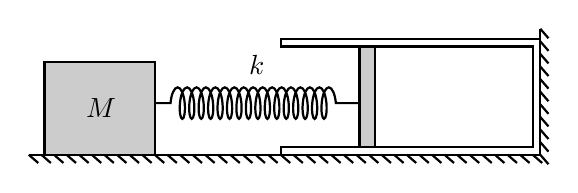
\begin{tikzpicture}[thick, scale = 0.8]
            % Ceiling with hatching
            \draw[thick] (0, 0.28) -- (8.12, 0.28);
            \foreach \x in {0,0.2,...,8.12}
                \draw (\x, 0.28) -- (\x+0.15, 0.15);
            \draw[thick] (8.12, 0.28) -- (8.12, 2.28);
            \foreach \x in {0.28,0.48,...,2.28}
                \draw (8.12, \x) -- (8.25, \x - 0.15);
            
            % Spring
            \draw [decoration={coil, aspect=0.3, segment length=1.2mm, amplitude=2mm, pre length=2mm, post length=2mm}, decorate, thick] (2, 1.1) -- (5.25, 1.1) node[midway,above=0.225cm]{$k$}; 
            
            % Shaded piston
            \draw[fill=gray!40] (5.25, 0.4) rectangle (5.5, 2);

            % M
            \draw[fill=gray!40] (0.25, 0.28) rectangle (2, 1.75) node[midway] {$M$};       
            
            % Cylinder walls (U-shaped container)
            \draw[thick] (4, 0.28) -- (8.12, 0.28) -- (8.12, 2.12) -- (4, 2.12) -- (4, 2) -- (8, 2) -- (8, 0.4) -- (4, 0.4) -- (4, 0.28);
        \end{tikzpicture}
    }}
    \begin{chc}
        Khi vật nặng $M$ bắt đầu dịch chuyển thì áp suất của khí trong cylinder bằng bao nhiêu $\mathrm{kPa}$?
        \shortans{104}
        \loigiai{Khi vật $M$ bắt đầu dịch chuyển, khi này lực đàn hồi của lò xo có độ lớn:\\
        ${F_{dh} = F_{ms} = \mu Mg = 0{,}2 \cdot 5 \cdot 10 = 10 \, \mathrm{N}}$\\
        Để piston bắt đầu dịch chuyển thì áp suất khí trong trường hợp này\\
        ${\Rightarrow p = p_0 + \frac{F_{dh}}{S} = 10^5 + \frac{10}{25 \cdot 10^{-4}} = 104 \cdot 10^3 \, \mathrm{Pa} = 104 \, \mathrm{kPa}}$.}
    \end{chc}

    \begin{chc}
        Nhiệt độ của khí trong cylinder tại thời điểm vật $M$ bắt đầu dịch chuyển bằng bao nhiêu Kelvin (làm tròn kết quả đến chữ số hàng đơn vị)?
        \shortans{390}
        \loigiai{Khi $M$ bắt đầu dịch chuyển, piston đã dịch chuyển được một đoạn:\\
        ${F_{dh} = k \Delta l \Rightarrow \Delta l = \frac{F_{dh}}{k} = \frac{10}{100} = 0{,}1 \, \mathrm{m} = 10 \, \mathrm{cm}}$\\
        Áp dụng phương trình trạng thái khí lí tưởng cho khối khí bên trong cylinder tại thời điểm ban đầu và tại thời điểm vật $M$ bắt đầu dịch chuyển:\\
        ${\frac{pV}{T} = \mathrm{const} \Rightarrow \frac{p_0 S l_0}{T_0} = \frac{p S \left(l_0 + \Delta l\right)}{T} \Rightarrow \frac{10^5 \cdot 40}{27 + 273} = \frac{104 \cdot 10^3 \cdot \left(40 + 10\right)}{T} \Rightarrow T = 390 \, \mathrm{K}}$.}
    \end{chc}
\end{ex}
% Câu 1
\begin{ex}
    Đồng hồ đo điện (công-tơ điện) lắp ở mỗi hộ dân dùng để đo
    \choice
    {công suất tiêu thụ điện năng}
    {công suất hao phí điện năng}
    {\True lượng điện năng tiêu thụ}
    {hiệu suất sử dụng điện}
    \loigiai{
        Lượng điện năng tiêu thụ.
    }
\end{ex}


% Câu 2
\begin{ex}
    Khi so sánh với sóng cơ học, sóng điện từ có điểm nào khác biệt?
    \choice
    {Có thể bị phản xạ, khúc xạ, giao thoa}
    {Mang năng lượng}
    {Là sóng ngang}
    {\True Truyền được trong chân không}
    \loigiai{
        Sóng cơ học không truyền được trong chân không, sóng điện từ truyền được trong chân không.
    }
\end{ex}


% Câu 3
\begin{ex}
    Trong các phản ứng hạt nhân sau đây, phản ứng nào không thể là phản ứng hạt nhân nhân tạo?
    \choice
    {${^4_2\mathrm{He}} + {^{27}_{13}\mathrm{Al}} \to {^{30}_{15}\mathrm{P}} + \mathrm{n}$}
    {${^2_1\mathrm{D}} + {^3_1\mathrm{T}} \to {^4_2\mathrm{He}} + \mathrm{n}$}
    {${^{235}_{92}\mathrm{U}} + \mathrm{n} \to {^{95}_{39}\mathrm{Y}} + {^{138}_{53}\mathrm{I}} + {3}\mathrm{n}$}
    {\True ${^{14}_6\mathrm{C}} \to {^{14}_7\mathrm{N}} + {^0_{-1}\mathrm{e}}$}
    \loigiai{
        Phản ứng D là phóng xạ nên không phải nhân tạo.
    }
\end{ex}


% Câu 4
\begin{ex}
    Hiện tượng phóng xạ không được sử dụng trong trường hợp nào dưới đây?
    \choice
    {Điều trị bệnh ung thư}
    {Xác định tuổi của các cổ vật bằng gỗ}
    {\True Siêu âm tim phổi và nội tạng}
    {Dùng làm chất đánh dấu trong Sinh học và Y học}
    \loigiai{
        Siêu âm tim phổi và nội tạng không sử dụng hiện tượng phóng xạ.
    }
\end{ex}


% Câu 5
\begin{ex}
    Ta thường ngửi được mùi thơm từ một tô phở nóng trong không khí ngào ngạt hơn so với một tô phở đã nguội. Theo thuyết động học phân tử chất khí, hiện tượng này được giải thích chủ yếu là do ở nhiệt độ cao, các phân tử hương liệu
    \choice
    {\True chuyển động hỗn loạn càng nhanh}
    {giãn nở và kích thước lớn hơn}
    {tương tác hút nhau mạnh hơn}
    {tập trung lại gần nhau hơn}
    \loigiai{
        Các phân tử khí chuyển động hỗn loạn, không ngừng. Khi nhiệt độ cao, các phân tử sẽ chuyển động nhanh hơn, khiến cho hiện tượng khuếch tán mạnh hơn.
    }
\end{ex}


% Câu 6
\begin{ex}
    Đâu là quan sát đúng về các hạt $\alpha$ trong thí nghiệm tán xạ hạt $\alpha$ của Rutherford?
    \choice
    {Tất cả đều xuyên qua lá vàng}
    {\True Hầu hết đi qua lá vàng, một số bị lệch đi một góc lớn, và một số thậm chí còn bị bật trở lại}
    {Hầu hết bị lệch bị lệch đi một một góc lớn, một số thậm chí còn bị bật trở lại và chỉ có một số rất nhỏ đi qua lá vàng}
    {Tất cả đều bị lệch đi rất nhiều}
    \loigiai{
        Hầu hết đi qua lá vàng, một số bị lệch đi một góc lớn, và một số thậm chí còn bị bật trở lại.
    }
\end{ex}


% Câu 7
\begin{ex}
    Khi nói về hiện tượng nóng chảy của một lượng chất rắn tinh thể xác định, nhận xét nào dưới đây là sai?
    \choice
    {Nhiệt độ của lượng chất không thay đổi}
    {\True Thế năng tương tác trung bình phân tử của lượng chất không đổi}
    {Nội năng của lượng chất tăng}
    {Động năng trung bình phân tử của lượng chất không đổi}
    \loigiai{
        Nhận nhiệt $\Rightarrow$ nội năng tăng (1). Nhiệt độ không đổi $\Rightarrow$ động năng trung bình không đổi (2). Từ (1) và (2) $\Rightarrow$ thế năng phân tử tăng.
    }
\end{ex}


% Câu 8
\begin{ex}
    Khi nói về nội năng của một vật, phát biểu nào sau đây là đúng?
    \choice
    {Các vật khác nhau có cùng nội năng nếu nhiệt độ của chúng bằng nhau}
    {Khi tốc độ của vật tăng thì động năng trung bình của các phân tử tăng và nội năng cũng tăng}
    {Khi vật rắn kết tinh nóng chảy, nhiệt độ không thay đổi nên nội năng cũng không thay đổi}
    {\True Việc thực hiện công trên vật hoặc truyền nhiệt cho vật có thể làm thay đổi nội năng của vật đó}
    \loigiai{
        Việc thực hiện công trên vật hoặc truyền nhiệt cho vật có thể làm thay đổi nội năng của vật đó.
    }
\end{ex}


% Câu 9
\begin{ex}
\immini[thm]{
        Cho một lượng chất dạng tinh thể tinh khiết vào trong nhiệt lượng kế và đun nóng nó bằng một sợi đốt với công suất cấp nhiệt không đổi. Dạng đồ thị phụ thuộc của nhiệt độ $(T)$ theo thời gian đun $(t)$ được cho trên hình vẽ. Nhận xét nào sau đây là sai?
        \choice
        {Từ $(1)$ đến $(2)$ là quá trình nóng chảy của chất rắn}
        {Từ $(2)$ đến $(3)$ là tăng nhiệt độ chất lỏng}
        {Từ $(3)$ đến $(4)$ là quá trình sôi của chất lỏng}
        {\True Từ $(4)$ đến $(5)$ là quá trình hóa hơi của chất lỏng}
    }{
        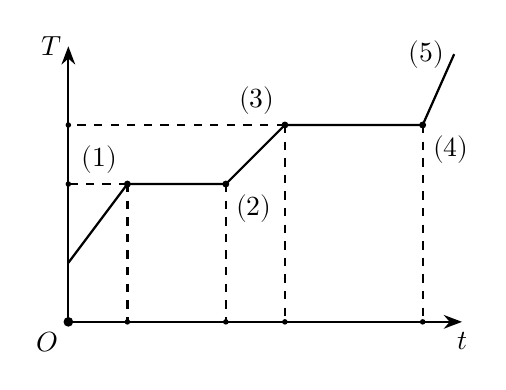
\begin{tikzpicture}[>=Stealth, thick, scale = 0.5]
            % --- 1. HỆ TRỤC TỌA ĐỘ ---
            \draw[->] (0,0) -- (10,0) node[below] {$t$};
            \draw[->] (0,0) -- (0,7) node[left] {$T$};
            \fill (0,0) circle (3.5pt) node[below left] {$O$};

            % --- 2. CÁC ĐIỂM DỮ LIỆU ---
            % Định nghĩa các tọa độ (x, y) để dễ quản lý
            \coordinate (Start) at (0,1.5);
            \coordinate (P1) at (1.5, 3.5);
            \coordinate (P2) at (4, 3.5);
            \coordinate (P3) at (5.5, 5);
            \coordinate (P4) at (9, 5);
            \coordinate (End) at (9.8, 6.8);

            % --- 3. VẼ ĐƯỜNG ĐỒ THỊ ---
            \draw[thick] (Start) -- (P1) -- (P2) -- (P3) -- (P4) -- (End);

            % --- 4. CÁC ĐƯỜNG GIÓNG (DOTTED) VÀ CÁC NỐT (DOTS) ---
            % Điểm 1
            \draw[dashed] (P1) -- (1.5,0);
            \draw[dashed] (P1) -- (0, 3.5);
            \fill (P1) circle (2.5pt) node[above left] {$(1)$};
            \fill (1.5, 0) circle (2pt);
            \fill (0, 3.5) circle (2pt);

            % Điểm 2
            \draw[dashed] (P2) -- (4,0);
            \fill (P2) circle (2.5pt) node[below right] {$(2)$};
            \fill (4, 0) circle (2pt);

            % Điểm 3
            \draw[dashed] (P3) -- (5.5,0);
            \draw[dashed] (P3) -- (0, 5);
            \fill (P3) circle (2.5pt) node[above left] {$(3)$};
            \fill (5.5, 0) circle (2pt);
            \fill (0, 5) circle (2pt);

            % Điểm 4
            \draw[dashed] (P4) -- (9,0);
            \fill (P4) circle (2.5pt) node[below right] {$(4)$};
            \fill (9, 0) circle (2pt);

            % Nhãn (5)
            \node at (End) [left] {$(5)$};

        \end{tikzpicture}
    }
    \loigiai{
        Từ $(4)$ đến $(5)$ là quá trình chất khí tăng nhiệt độ.
    }
\end{ex}


% Câu 10
\begin{ex}
\immini[thm]{
        Để bảo vệ người dùng khỏi nguy cơ bị điện giật khi chạm vào vỏ kim loại của các thiết bị điện, người ta thường dùng một dây kim loại để nối từ vỏ thiết bị xuống đất (gọi là dây tiếp đất). Hình vẽ bên cho thấy vỏ kim loại của một thiết bị điện đang tích điện dương, nhưng nhờ được nối đất mà vỏ kim loại nhanh chóng trở nên trung hòa về điện, không còn nguy hiểm với người dùng nữa. Cơ chế của hiện tượng
    }{
        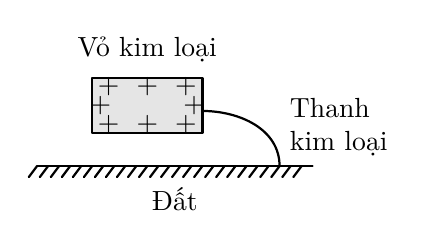
\begin{tikzpicture}[line join=round, line cap=round, thick, scale = 0.7]
            % --- 1. VẼ MẶT ĐẤT ---
            \draw[thick] (-1,0) -- (4,0); % Đường nằm ngang
            \foreach \x in {-1, -0.8, ..., 3.8} {
                \draw (\x,0) -- (\x-0.15, -0.2); % Các vạch gạch chéo
            }
            \node[below] at (1.5, -0.2) {Đất};

            % --- 2. VẼ VỎ KIM LOẠI (RECTANGLE) ---
            \filldraw[fill=gray!20] (0,0.6) rectangle (2,1.6);
            \node[above] at (1, 1.7) {Vỏ kim loại};

            % --- 3. CÁC DẤU ĐIỆN TÍCH DƯƠNG (+) ---
            % Hàng trên
            \node[] at (0.3, 1.45) {+};
            \node[] at (1.0, 1.45) {+};
            \node[] at (1.7, 1.45) {+};
            % Hai bên
            \node[] at (0.15, 1.1) {+};
            \node[] at (1.85, 1.1) {+};
            % Hàng dưới
            \node[] at (0.3, 0.75) {+};
            \node[] at (1.0, 0.75) {+};
            \node[] at (1.7, 0.75) {+};

            % --- 4. THANH KIM LOẠI NỐI ĐẤT ---
            \draw[] (2,1) to[out=0, in=90] (3.4, 0) node[above right, align=left] {Thanh \\ kim loại};

        \end{tikzpicture}
    }
    \choice
    {các điện tích dương di chuyển từ vỏ kim loại xuống lòng đất}
    {các điện tích dương di chuyển từ lòng đất lên vỏ kim loại}
    {\True các điện tích âm di chuyển từ lòng đất lên vỏ kim loại}
    {các điện tích âm di chuyển từ vỏ kim loại xuống lòng đất}
    \loigiai{
        Các điện tích âm di chuyển từ lòng đất lên vỏ kim loại.
    }
\end{ex}


% Câu 11
\begin{ex}
\immini[thm]{
        Một dây dẫn thẳng dài vô hạn mang dòng điện $I$ và một khung dây hình chữ nhật cùng nằm trên mặt phẳng trang giấy như hình vẽ. Khi cường độ dòng điện $I$ giảm, khung dây hình chữ nhật sẽ
        \choice
        {\True dịch chuyển sang trái}
        {dịch chuyển sang phải}
        {đứng yên}
        {quay}
    }{
        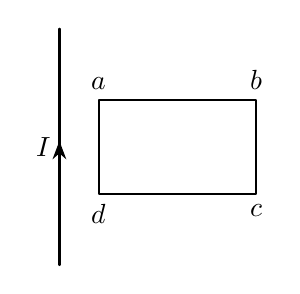
\begin{tikzpicture}[thick, line join=round, line cap=round, >=Stealth, yscale = 0.75, scale=1]
            % 1. Vẽ dây dẫn thẳng đứng và dòng điện I
            \draw[thick] (0,-2) -- (0,2);
            \draw[thick, ->] (0,0) -- (0,0.1); % Mũi tên chỉ chiều dòng điện
            \node[left] at (0,0) {$I$};

            % 2. Vẽ khung dây dẫn hình chữ nhật abcd
            \draw[thick] (0.5, -0.8) rectangle (2.5, 0.8);

            % 3. Thêm các nhãn đỉnh a, b, c, d
            \node[above] at (0.5, 0.8) {$a$};
            \node[above] at (2.5, 0.8) {$b$};
            \node[below] at (2.5, -0.8) {$c$};
            \node[below] at (0.5, -0.8) {$d$};
        \end{tikzpicture}
    }
    \loigiai{
        Khi $I$ giảm thì $B$ giảm $\Rightarrow$ từ thông giảm $\Rightarrow$ khung dây có xu hướng lại gần dòng điện để chống lại sự giảm từ thông.
    }
\end{ex}


% Câu 12
\begin{ex}
    Một khối khí lí tưởng nhất định đang ở trạng thái ban đầu nhất định. Bây giờ chúng ta muốn làm cho nhiệt độ của nó trở lại nhiệt độ của trạng thái ban đầu sau khi trạng thái thay đổi thì quá trình nào sau đây có thể được sử dụng?
    \choice
    {\True Đầu tiên, giữ áp suất không đổi và tăng thể tích, sau đó giữ thể tích không đổi và giảm áp suất}
    {Đầu tiên, giữ áp suất không đổi và giảm thể tích, sau đó giữ thể tích không đổi và giảm áp suất}
    {Đầu tiên, giữ thể tích không đổi và tăng áp suất, sau đó giữ áp suất không đổi và tăng thể tích}
    {Đầu tiên, giữ thể tích không đổi và giảm áp suất, sau đó giữ áp suất không đổi và giảm thể tích}
    \loigiai{
        Xét đáp án A có $p$ không đổi và $V$ tăng $\Rightarrow T$ tăng, sau đó $V$ không đổi và $p$ giảm $\Rightarrow T$ giảm.
    }
\end{ex}


% Câu 13
\begin{ex}
\immini[thm]{
        Như hình bên, một thanh nam châm chuyển động dọc theo trục của một vòng dây từ phía trên và đi qua vòng dây với tốc độ không đổi. Tâm của nam châm đồng phẳng với vòng dây tại thời điểm $t_1$. Quy ước dòng điện có chiều ngược chiều kim đồng hồ khi nhìn từ trên xuống là chiều dương. Đồ thị biểu diễn sự thay đổi của cường độ dòng điện trong vòng dây theo thời gian $t$ là
    }{
        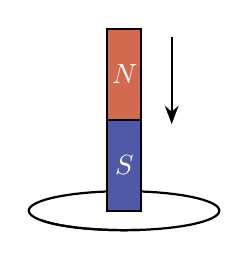
\begin{tikzpicture}[scale=0.55, >=Stealth, thick]
            \definecolor{magRed}{RGB}{210, 106, 79}
            \definecolor{magBlue}{RGB}{80, 89, 168}
            % Vòng dây elip: tâm x = 0.8/2 = 0.4, bán kính x=2.2cm, y=0.45cm
            \draw[thick] (0.4, 0) ellipse (2.2cm and 0.45cm);
            % Nam châm: rộng 0.8, cao mỗi cực 2.1
            \filldraw[fill=magBlue, draw=black, thick] (0,0) rectangle (0.8, 2.1) node[pos=0.5, white]{$S$};
            \filldraw[fill=magRed, draw=black, thick] (0, 2.1) rectangle (0.8, 4.2) node[pos=0.5, white]{$N$};
            % Mũi tên chỉ chiều dòng điện
            \draw[-, thick] (0.4,0) ++(225-15:2.2cm and 0.45cm) arc (210 : 280 : 2.2cm and 0.45cm);
            % Mũi tên chỉ chiều chuyển động của nam châm (hướng xuống)
            \draw[<-, thick] (1.5cm, 2) -- (1.5cm, 4);
        \end{tikzpicture}
    }
    \choice
    {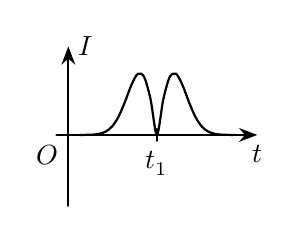
\begin{tikzpicture}[>=Stealth, line cap=round, line join=round, thick, scale = 0.75, black]
                % Định nghĩa hàm số mô phỏng xung dòng điện (Đạo hàm của hàm Gauss để ra dạng chuẩn vật lý)
                % f(x) = (x-1.5) * exp(-5*(x-1.5)^2)
                % --- Đồ thị A: Hai xung dương (Trị tuyệt đối) ---
                \draw[->] (-0.2,0) -- (3.2,0) node[below] {$t$};
                \draw[->] (0,-1.2) -- (0,1.5) node[right] {$I$};
                \node[below left] at (0,0) {$O$};
                \draw[thick] (1.5, 0.1) -- (1.5, -0.1) node[below] {$t_1$};
                \draw[smooth, domain=0.2:2.8] 
                    plot (\x, {6*abs((\x-1.5)*exp(-6*(\x-1.5)^2))});
            \end{tikzpicture}}
    {\begin{tikzpicture}[>=Stealth, line cap=round, line join=round, thick, scale = 0.75, black]
                % Định nghĩa hàm số mô phỏng xung dòng điện (Đạo hàm của hàm Gauss để ra dạng chuẩn vật lý)
                % f(x) = (x-1.5) * exp(-5*(x-1.5)^2)
                % --- Đồ thị B: Xung dương trước, xung âm sau (Đáp án đúng nếu N rơi xuống) ---
                \draw[->] (-0.2,0) -- (3.2,0) node[below] {$t$};
                \draw[->] (0,-1.2) -- (0,1.5) node[right] {$I$};
                \node[below left] at (0,0) {$O$};
                \draw[thick] (1.5, 0.1) -- (1.5, -0.1) node[below left] {$t_1$};
                \draw[smooth, domain=0.2:2.8] 
                    plot (\x, {-8*(\x-1.5)*exp(-6*(\x-1.5)^2)});
            \end{tikzpicture}}
    {\begin{tikzpicture}[>=Stealth, line cap=round, line join=round, thick, scale = 0.75, black]
                % Định nghĩa hàm số mô phỏng xung dòng điện (Đạo hàm của hàm Gauss để ra dạng chuẩn vật lý)
                % f(x) = (x-1.5) * exp(-5*(x-1.5)^2)
                % --- Đồ thị C: Một xung dương duy nhất ---
                \draw[->] (-0.2,0) -- (3.2,0) node[below] {$t$};
                \draw[->] (0,-1.2) -- (0,1.5) node[right] {$I$};
                \node[below left] at (0,0) {$O$};
                \draw[thick] (1.5, 0.1) -- (1.5, -0.1) node[below] {$t_1$};
                \draw[smooth, domain=0.2:2.8] 
                    plot (\x, {1.2*exp(-10*(\x-1.5)^2)});
            \end{tikzpicture}}
    {\True \begin{tikzpicture}[>=Stealth, line cap=round, line join=round, thick, scale = 0.75, black]
                % Định nghĩa hàm số mô phỏng xung dòng điện (Đạo hàm của hàm Gauss để ra dạng chuẩn vật lý)
                % f(x) = (x-1.5) * exp(-5*(x-1.5)^2)
                % --- Đồ thị D: Xung âm trước, xung dương sau ---
                \draw[->] (-0.2,0) -- (3.2,0) node[below] {$t$};
                \draw[->] (0,-1.2) -- (0,1.5) node[right] {$I$};
                \node[below left] at (0,0) {$O$};
                \draw[thick] (1.5, 0.1) -- (1.5, -0.1) node[below right] {$t_1$};
                \draw[smooth, domain=0.2:2.8] 
                    plot (\x, {8*(\x-1.5)*exp(-6*(\x-1.5)^2)});
            \end{tikzpicture}}
    \loigiai{
        Theo quy tắc vào nam ra bắc (vào $S$ ra $N$) thì $\overrightarrow{B}$ ban đầu hướng lên. Khi nam châm lại gần vòng dây thì từ thông tăng $\Rightarrow \overrightarrow{B_{cu}} \uparrow \downarrow \overrightarrow{B} \Rightarrow \overrightarrow{B_{cu}}$ hướng xuống. Áp dụng quy tắc nắm tay phải được chiều dòng điện cùng chiều kim đồng hồ, tức là ngược chiều dương quy ước $\Rightarrow i < 0$.
    }
\end{ex}


% Câu 14
\begin{ex}
\immini[thm]{
        Theo giản đồ pha của nước ở hình bên, nhận xét nào sau đây là sai?
        \choice
        {Trong điều kiện áp suất bằng ${550} \, \mathrm{Pa}$, hơi nước không thể hóa lỏng}
        {\True Tại nhiệt độ nhỏ hơn ${0{,}01} \, \mathrm{^\circ C}$, hơi nước không thể ngưng kết}
        {Trong điều kiện áp suất bằng ${700} \, \mathrm{Pa}$, nước đá không thể thăng hoa}
        {Tại nhiệt độ lớn hơn ${0{,}01} \, \mathrm{^\circ C}$, nước không thể đông đặc}
    }{
        \begin{tikzpicture}[scale=0.5, line cap=round, line join=round, thick]
            % --- 1. KHUNG ĐỒ THỊ ---
            \draw[thick] (0,0) rectangle (7,6);

            % --- 2. TRỤC TỌA ĐỘ VÀ NHÃN ---
            \node[rotate=90, above] at (0, 4.5) {$p \, \mathrm{(Pa)}$};
            \node at (5.5, 0) [below] {$t \, \mathrm{(^\circ C)}$};

            % Định nghĩa tọa độ điểm ba (Triple Point)
            \coordinate (TP) at (2.8, 2.2);

            % --- 3. CÁC ĐƯỜNG RANH GIỚI PHA ---
            % Đường thăng hoa (Rắn - Hơi): cong nhẹ từ gốc lên
            \draw[thick] (0, 0) to[out=20, in=240] (TP);
            
            % Đường nóng chảy (Rắn - Lỏng): nghiêng nhẹ sang trái (đặc trưng của nước)
            \draw[thick] (2.2, 6) -- (TP);
            
            % Đường hóa hơi (Lỏng - Hơi): đường cong đi lên mạnh
            \draw[thick] (TP) to[out=20, in=255] (6.4, 6);

            % --- 4. ĐƯỜNG GIÓNG VÀ SỐ LIỆU ---
            % Gióng xuống trục Nhiệt độ
            \draw[thick, dashed] (TP) -- (2.8, 0);
            \node[below] at (2.8, 0) {0,01};

            % Gióng sang trục Áp suất
            \draw[thick, dashed] (TP) -- (0, 2.2);
            \node[left] at (0, 2.2) {611,73};

            % --- 5. TÊN CÁC VÙNG PHA ---
            \node[align=center] at (1.15, 3.8) {Nước\\đá};
            \node at (3.9, 4.5) {Nước};
            \node at (5, 1.5) {Hơi nước};

        \end{tikzpicture}
    }
    \loigiai{
        Trong điều kiện áp suất bằng ${550} \, \mathrm{Pa}$, hơi nước chỉ có thể ngưng kết. Tại nhiệt độ lớn hơn ${0{,}01} \, \mathrm{^\circ C}$, hơi nước không thể ngưng kết.
    }
\end{ex}


% Câu 15
\begin{ex}
    Phát biểu nào sau đây là đúng về nhiệt độ và sự truyền nhiệt?
    \choice
    {Với tiến bộ của khoa học, nhiệt độ ${-280} \, \mathrm{^\circ C}$ đã đạt được trong thực tế}
    {Vật có nhiệt độ tăng thêm ${3} \, \mathrm{^\circ C}$, cũng có nghĩa tăng thêm ${276} \, \mathrm{K}$}
    {\True Hệ hai vật $A$ và $B$ đạt trạng thái cân bằng nhiệt vì nhiệt độ của chúng bằng nhau}
    {Hai vật có nội năng khác nhau cho tiếp xúc thì chúng luôn truyền nhiệt cho nhau}
    \loigiai{
        Nhiệt độ ${-280} \, \mathrm{^\circ C} < {-273} \, \mathrm{^\circ C} \approx {0} \, \mathrm{K}$ không đạt được trong thực tế $\Rightarrow$ A Sai. \\
        Vật có nhiệt độ tăng thêm ${3} \, \mathrm{^\circ C}$, cũng có nghĩa tăng thêm ${3} \, \mathrm{K} \Rightarrow$ B Sai. \\
        Hai vật có nội năng khác nhau nhưng nhiệt độ vẫn có thể bằng nhau $\Rightarrow$ D Sai.
    }
\end{ex}


% Câu 16
\begin{ex}
    Bán kính Trái Đất là ${6{,}4 \cdot 10^3} \, \mathrm{km}$, khối lượng mol của nước là ${18} \, \mathrm{g/mol}$. Giả sử ${1} \, \mathrm{kg}$ nước phân bố đều trên bề mặt Trái Đất; khi đó, số phân tử nước phân bố trên ${1} \, \mathrm{cm^2}$ bề mặt Trái Đất là
    \choice
    {${6{,}5 \cdot 10^3}$}
    {\True ${6{,}5 \cdot 10^6}$}
    {${6{,}5 \cdot 10^{10}}$}
    {${6{,}5 \cdot 10^{12}}$}
    \loigiai{
        $n = \frac{m}{M} = \frac{10^3}{18} = \frac{500}{9} \, \mathrm{mol}$.\\
        $N = n N_A \cdot \frac{S}{4\pi R^2} = \frac{500}{9} \cdot 6{,}02 \cdot 10^{23} \cdot \frac{10^{-4}}{4\pi \cdot \left(6{,}4 \cdot 10^6\right)^2} \approx 6{,}5 \cdot 10^6$.
    }
\end{ex}


% Câu 17
\begin{ex}
    Cho một proton chuyển động vào trong một điện trường đều có cường độ ${5 \cdot 10^4} \, \mathrm{V/m}$ theo phương vuông góc với các đường sức của điện trường với tốc độ ${10^5} \, \mathrm{m/s}$. Để quỹ đạo của proton vẫn là một đường thẳng thì phải đặt thêm một từ trường đều với độ lớn của véc-tơ cảm ứng từ là
    \choice
    {${0{,}1} \, \mathrm{T}$}
    {${0{,}3} \, \mathrm{T}$}
    {\True ${0{,}5} \, \mathrm{T}$}
    {${0{,}8} \, \mathrm{T}$}
    \loigiai{
        $F_B = F_E \Rightarrow qBv = qE \Rightarrow B = \frac{E}{v} = \frac{5 \cdot 10^4}{10^5} = 0{,}5 \, \mathrm{T}$.
    }
\end{ex}


% Câu 18
\begin{ex}
    Ban đầu có một mẫu phóng xạ nguyên chất, sau thời gian $\tau$ số hạt nhân chất phóng xạ giảm đi $e$ lần ($e$ là cơ số của loga tự nhiên với $\ln e = 1$). Sau thời gian $3\tau$ thì khối lượng chất phóng xạ trong mẫu còn lại bao nhiêu phần trăm so với ban đầu?
    \choice
    {${25}\%$}
    {${12{,}5}\%$}
    {${15}\%$}
    {\True ${5}\%$}
    \loigiai{
        $N = N_0 e^{-\lambda t} \Rightarrow e^{-1} = e^{-\lambda \tau} \Rightarrow \tau = \frac{1}{\lambda}$.\\
        $\frac{m}{m_0} = e^{-\lambda \cdot 3\tau} = e^{-\lambda \cdot \frac{3}{\lambda}} = e^{-3} \approx 0{,}05 = 5\%$.
    }
\end{ex}


% Câu 1
\begin{ex}
    Pin hạt nhân đang thu hút sự quan tâm lớn nhờ khả năng cung cấp năng lượng liên tục trong nhiều thập kỉ mà không cần sạc và hoạt động ổn định trong các điều kiện môi trường khắc nghiệt. Loại pin này thường được ứng dụng trong lĩnh vực hàng không vũ trụ và y tế. Một mẫu pin hạt nhân sử dụng năng lượng từ sự phân rã của đồng vị phóng xạ Niken (${^{63}_{28}\mathrm{Ni}}$). Biết ${^{63}_{28}\mathrm{Ni}}$ là chất phóng xạ $\beta^-$, có chu kì bán rã là ${100}$ năm và biến thành đồng vị bền của Đồng.
    \choiceTF[1]
    {Vỏ của mẫu pin hạt nhân chỉ cần bao bọc bằng một lớp giấy mỏng là đủ để ngăn cản bức xạ, đảm bảo an toàn khi sử dụng}
    {Phương trình phân rã trong quá trình này là ${^{63}_{28}\mathrm{Ni}} \to {^{63}_{27}\mathrm{Cu}} + \beta^-$}
    {\True Sau ${100}$ năm hoạt động khối lượng Niken còn lại trong pin bằng ${50}\%$ khối lượng ban đầu}
    {\True Máy tạo nhịp tim chỉ hoạt động ổn định khi độ phóng xạ của pin còn ít nhất ${75}\%$ so với ban đầu. Nếu cấy ghép thiết bị này cho một bệnh nhân ${50}$ tuổi, thì đến trước khi bệnh nhân thọ ${91}$ tuổi máy vẫn đảm bảo hoạt động an toàn}
    \loigiai{
        \begin{itemchoice}
        \itemch Tia $\beta^-$ xuyên được qua giấy mỏng nên vỏ pin phải được bọc bằng nhôm
        \itemch ${^{63}_{28}\mathrm{Ni}} \to {^{63}_{29}\mathrm{Cu}} + \beta^-$
        \itemch Sau 1 chu kì thì khối lượng còn một nửa
        \itemch $H = H_0 \cdot 2^{-\frac{t}{T}} \Rightarrow 0{,}75 = 2^{-\frac{t}{100}} \Rightarrow t \approx 41{,}5$ năm
        \end{itemchoice}
    }
\end{ex}


% Câu 2
\begin{ex}
\immini[thm]{
        Thí nghiệm ``cân dòng điện'' được thiết kế như hình vẽ. Dòng điện qua dây dẫn được cấp từ một nguồn phát dòng điện một chiều đặc biệt. Nguồn điện này cho phép điều chỉnh cường độ dòng điện và có thể đảo ngược chiều dòng điện bằng cách bật một công tắc trên nguồn. Một học sinh đã thực hiện thí nghiệm theo ba bước sau: \\
        (I) Chỉnh cân về giá trị ${0}$, đặt nam châm lên cân, lắp đặt dây điện và nối hai đầu dây vào nguồn điện;\\
        (II) bật nguồn và điều chỉnh cường độ dòng điện tới giá trị $I$ xác định, quan sát thấy cân chỉ ${457} \, \mathrm{g}$;\\
        (III) giữ nguyên cường độ dòng điện $I$ nhưng đảo chiều dòng điện theo hướng ngược lại thì quan sát thấy cân chỉ ${538} \, \mathrm{g}$. \\
        Cho gia tốc trọng trường $g = {9{,}8} \, \mathrm{m/s^2}$.
    }{
        \begin{tikzpicture}[line join=round, line cap=round, >=Stealth, yscale=-1, thick, scale = 0.115]
            \definecolor{magRed}{RGB}{210, 106, 79}
            \definecolor{magBlue}{RGB}{80, 89, 168}
            % --- ĐỊNH NGHĨA TỌA ĐỘ CÁC ĐIỂM CHÍNH ---
            
            % Cân điện tử (Thân chính)
            \coordinate (C1) at (43.5,51.0); 
            \coordinate (C2) at (46.5,60.0); 
            \coordinate (C3) at (65.0,49.0);
            \coordinate (C4) at (62.0,40.0);
            \coordinate (C5) at (46.5,62.5); 
            \coordinate (C6) at ($(C5)+(C3)-(C2)$); 
            \coordinate (C7) at (22.0,38.0); 
            \coordinate (C8) at (22.0,47.0); 
            \coordinate (C9) at (40.0,27.0); 

            % ===== VECTOR MẶT TRÊN =====
            \coordinate (uTop) at ($(C4)-(C1)$); % hướng ngang mặt trên
            \coordinate (vTop) at ($(C7)-(C1)$); % hướng dọc mặt trên
            \coordinate (wTop) at ($(0,-1)$); % hướng từ dưới lên trên

            % ===== CHÂN ĐẾ 1 =====
            \coordinate (S1) at (27.0,65.0);
            
            \coordinate (S1B1) at ($(S1) + 0.0*(uTop) + 0.0*(vTop)$);
            \coordinate (S1B2) at ($(S1) + 0.5*(uTop) + 0.0*(vTop)$);
            \coordinate (S1B3) at ($(S1) + 0.5*(uTop) + 0.5*(vTop)$);
            \coordinate (S1B4) at ($(S1) + 0.0*(uTop) + 0.5*(vTop)$);
            
            % ===== CHÂN ĐẾ 2 =====
            \coordinate (S2) at (55.0,45.0);
            
            \coordinate (S2B1) at ($(S2) + 0.0*(uTop) + 0.0*(vTop)$);
            \coordinate (S2B2) at ($(S2) + 0.5*(uTop) + 0.0*(vTop)$);
            \coordinate (S2B3) at ($(S2) + 0.5*(uTop) + 0.5*(vTop)$);
            \coordinate (S2B4) at ($(S2) + 0.0*(uTop) + 0.5*(vTop)$);

            % ===== VẼ ĐẾ =====
            \draw[fill=black!80] (S1B1)--(S1B2)--(S1B3)--(S1B4)--cycle;
            \draw[fill=black!80] (S2B1)--(S2B2)--(S2B3)--(S2B4)--cycle;
            
            % ===== TÂM ĐẾ =====
            \coordinate (S1Cen) at ($(S1B1)!0.5!(S1B3)$);
            \coordinate (S2Cen) at ($(S2B1)!0.5!(S2B3)$);
            
            % ===== CHIỀU CAO TRỤ =====
            \coordinate (h) at (0,-20);
            
            % ===== TRỤ 1 (hình chữ nhật) =====
            \coordinate (S1A) at ($(S1Cen) + (-0.5,0)$);
            \coordinate (S1B) at ($(S1Cen) + (0.5,0)$);
            \coordinate (S1C) at ($(S1Cen) + (0.5,0) + (h)$);
            \coordinate (S1D) at ($(S1Cen) + (-0.5,0) + (h)$);
            
            % ===== TRỤ 2 =====
            \coordinate (S2A) at ($(S2Cen) + (-0.5,0)$);
            \coordinate (S2B) at ($(S2Cen) + (0.5,0)$);
            \coordinate (S2C) at ($(S2Cen) + (0.5,0) + (h)$);
            \coordinate (S2D) at ($(S2Cen) + (-0.5,0) + (h)$);
            
            % ===== VẼ TRỤ 2 =====
            \draw[fill=gray!80] (S2A)--(S2B)--(S2C)--(S2D)--cycle;
            
            % Vẽ Thân Cân
            \draw[fill=gray!40] (C1) -- (C2) -- (C3) -- (C4) -- cycle; % Mặt Vát
            \draw[fill=gray!60] (C2) -- (C5) -- (C6) -- (C3) -- cycle;        % Mặt trước, dưới mặt vát
            \draw[fill=gray] (C1) -- (C2) -- (C5) -- (C8) -- (C7) -- cycle;        % Mặt bên
            \draw[fill=gray!50] (C1) -- (C4) -- (C9) -- (C7) -- cycle; % Mặt trên

            % ===== VECTOR HỆ MẶT VÁT =====
            \coordinate (u) at ($(C2)-(C1)$); % trục dọc
            \coordinate (v) at ($(C4)-(C1)$); % trục ngang
            
            % ===== MÀN HÌNH LCD =====
            \coordinate (L1) at ($(C1) + 0.20*(u) + 0.10*(v)$);
            \coordinate (L2) at ($(C1) + 0.65*(u) + 0.10*(v)$);
            \coordinate (L3) at ($(C1) + 0.65*(u) + 0.90*(v)$);
            \coordinate (L4) at ($(C1) + 0.20*(u) + 0.90*(v)$);
            
            % ===== NÚT BÊN TRÁI =====
            \coordinate (B11) at ($(C1) + 0.78*(u) + 0.15*(v)$);
            \coordinate (B12) at ($(C1) + 0.88*(u) + 0.15*(v)$);
            \coordinate (B13) at ($(C1) + 0.88*(u) + 0.3*(v)$);
            \coordinate (B14) at ($(C1) + 0.78*(u) + 0.3*(v)$);
            
            % ===== NÚT BÊN PHẢI =====
            \coordinate (B21) at ($(C1) + 0.78*(u) + 0.7*(v)$);
            \coordinate (B22) at ($(C1) + 0.88*(u) + 0.7*(v)$);
            \coordinate (B23) at ($(C1) + 0.88*(u) + 0.85*(v)$);
            \coordinate (B24) at ($(C1) + 0.78*(u) + 0.85*(v)$);
            % Vẽ Màn hình
            \draw[fill=white] (L1) -- (L2) -- (L3) -- (L4) -- cycle;
            \path let \p1 = (L1), \p2 = (L2) in;
            \node[rotate=30] at ($(L1)!0.5!(L3)$) {\footnotesize \textit{\textifsym{457}} ${g}$};

            % Nút bấm
            \draw[fill=gray] (B11) -- (B12) -- (B13) -- (B14) -- cycle;
            \draw[fill=black!70] (B21) -- (B22) -- (B23) -- (B24) -- cycle;
            
            % ===== HÌNH CHỮ NHẬT NHỎ TRÊN MẶT TRÊN =====
            \coordinate (T1) at ($(C1) + 0.2*(uTop) + 0.30*(vTop)$);
            \coordinate (T2) at ($(C1) + 0.8*(uTop) + 0.30*(vTop)$);
            \coordinate (T3) at ($(C1) + 0.8*(uTop) + 0.75*(vTop)$);
            \coordinate (T4) at ($(C1) + 0.2*(uTop) + 0.75*(vTop)$);
            
            \coordinate (T11) at ($(C1) + 0.2*(uTop) + 0.30*(vTop) + 10*(wTop)$);
            \coordinate (T12) at ($(C1) + 0.8*(uTop) + 0.30*(vTop) + 10*(wTop)$);
            \coordinate (T13) at ($(C1) + 0.8*(uTop) + 0.75*(vTop) + 10*(wTop)$);
            \coordinate (T14) at ($(C1) + 0.2*(uTop) + 0.75*(vTop) + 10*(wTop)$);
            
            % N
            \coordinate (N1) at ($(C1) + 0.3*(uTop) + 0.30*(vTop) + 4*(wTop)$);
            \coordinate (N2) at ($(C1) + 0.7*(uTop) + 0.30*(vTop) + 4*(wTop)$);
            \coordinate (N3) at ($(C1) + 0.7*(uTop) + 0.30*(vTop) + 9*(wTop)$);
            \coordinate (N4) at ($(C1) + 0.3*(uTop) + 0.30*(vTop) + 9*(wTop)$);
            
            % S
            \coordinate (S1) at ($(C1) + 0.7*(uTop) + 0.75*(vTop) + 4*(wTop)$);
            \coordinate (S2) at ($(C1) + 0.3*(uTop) + 0.75*(vTop) + 4*(wTop)$);
            \coordinate (S3) at ($(C1) + 0.3*(uTop) + 0.75*(vTop) + 9*(wTop)$);
            \coordinate (S4) at ($(C1) + 0.7*(uTop) + 0.75*(vTop) + 9*(wTop)$);
            
            % ===== VẼ =====
            \draw[fill=gray!30] (T1) -- (T2) -- (T3) -- (T4) -- cycle; % Đáy
            \draw[fill=gray!20] (T3) -- (T13) -- (T14) -- (T4) -- cycle; % Cạnh đứng trong
            \draw[fill=gray!20] (T1) -- (T11) -- (T12) -- (T2) -- cycle; % Cạnh đứng ngoài
            
            \draw[fill=magRed] (N1) -- (N2) -- (N3) -- (N4) -- cycle; % Tấm N
            \node[rotate=15, white] at ($(N1)!0.5!(N3)$) {${N}$};
            \draw[fill=magBlue] (S1) -- (S2) -- (S3) -- (S4) -- cycle; % Tấm S
            \node[rotate=15, white] at ($(S1)!0.5!(S3)$) {${S}$};
            
            % ===== VẼ TRỤ 1 =====
            \draw[fill=gray!80] (S1A)--(S1B)--(S1C)--(S1D)--cycle;
            
            % Vẽ Dây dẫn chính (Nối từ 2 thanh ngang)
            \draw[ultra thick, postaction={decorate, decoration={markings, mark=at position 0.5 with {\arrow{>}}}}] ($(S1Cen) + (0,-18)$) -- ($(S2Cen) + (0,-18)$);
            
            % Vẽ Dây điện nối ngoài
            \draw[ultra thick] ($(S1Cen) + (0,-18)$) .. controls (21,50) and (25,50) .. (20,65);
            \draw[ultra thick] ($(S2Cen) + (0,-18)$) .. controls (62,20) and (60,24) .. (65,35);
        \end{tikzpicture}
    }
    \choiceTF[1]
    {\True Thiết kế này cho phép kiểm chứng sự phụ thuộc của lực từ tác dụng lên dòng điện theo chiều của dòng điện và cường độ của dòng điện}
    {Khối lượng của cục nam châm là ${457} \, \mathrm{g}$}
    {\True Độ lớn lực từ tác dụng lên dòng điện có cường độ $I$ xấp xỉ bằng ${397} \, \mathrm{mN}$}
    {Với thiết kế thí nghiệm này, chỉ dựa vào số liệu trên, bạn học sinh có thể vận dụng công thức để tính được độ lớn cảm ứng từ của từ trường do nam châm tạo ra}
    \loigiai{
        \begin{itemchoice}
        \itemch 
        \itemch ${457} \, \mathrm{g}$ không phải khối lượng của nam châm
        \itemch Đổi chiều dòng điện $\Rightarrow$ lực từ đổi chiều $\Rightarrow$ chênh lệch $2F $\\
        $\Rightarrow 2F = \Delta m g = (538 - 457) \cdot 10^{-3} \cdot 9{,}8 \Rightarrow F = 0{,}3969 \, \mathrm{N} = 396{,}9 \, \mathrm{mN}$
        \itemch Chưa đủ số liệu, chẳng hạn như chiều dài đoạn dây
        \end{itemchoice}
    }
\end{ex}


% Câu 3
\begin{ex}
\immini[thm]{
        Một khối khí lí tưởng được chứa trong một xilanh với pit-tông có thể di chuyển không ma sát. Pit-tông có khối lượng ${100} \, \mathrm{g}$, tiết diện ${20} \, \mathrm{cm^2}$. Ban đầu, chiều cao và nhiệt độ của cột khí trong xilanh lần lượt là ${10} \, \mathrm{cm}$ và ${27} \, \mathrm{^\circ C}$. Người ta đun nóng từ từ khối khí trong xilanh đến nhiệt độ ${97} \, \mathrm{^\circ C}$. Áp suất khí quyển bằng ${10^5} \, \mathrm{Pa}$. Lấy $g = {10} \, \mathrm{m/s^2}$.
        \choiceTF[1]
        {\True Khi pit-tông cân bằng, áp suất của khối khí trong xilanh bằng ${100500} \, \mathrm{Pa}$}
        {Khối khí chứa trong xilanh có số mol xấp xỉ ${0{,}08} \, \mathrm{mol}$}
        {\True Công mà khối khí trong xilanh đã thực hiện bằng ${4{,}69} \, \mathrm{J}$}
        {\True Đồ thị biểu diễn mối liên hệ giữa thể tích và nhiệt độ tuyệt đối của khối khí trong hệ tọa độ $V - T$ là đường thẳng có đường kéo dài đi qua gốc tọa độ}

    }{
        \begin{tikzpicture}[line join=round, line cap=round, >=stealth, scale=0.7, thick]
        % Định nghĩa màu sắc
        \definecolor{liquidColor}{RGB}{210, 255, 210} % Xanh lá nhạt cho chất lỏng
        \definecolor{flameInner}{RGB}{255, 255, 100}
        \definecolor{flameOuter}{RGB}{255, 140, 0}

        % 1. MẶT ĐẤT VÀ GIÁ ĐỠ
        \draw[fill=black!80] (-0.5,-0.1) rectangle (3.5,0.1); % Mặt bàn
        \draw[thick] (0.2,0.1) -- (0.2,2.7) -- (2.8,2.7) -- (2.8,0.1); % Giá đỡ

        % 2. ĐÈN CỒN (SPIRIT LAMP)
        % Thân đèn
        \draw[thick, fill=gray!10] (0.8,0.1) .. controls (0.8,1.2) and (0.6,1.4) .. (1.0,1.8) 
            -- (2.0,1.8) .. controls (2.4,1.4) and (2.2,1.2) .. (2.2,0.1) -- cycle;
        % Bấc đèn bên trong
        \draw[thick] (1.4,1.8) .. controls (1.2,1.0) and (1.8,0.6) .. (1.0,0.4);
        \draw[thick] (1.6,1.8) .. controls (1.8,1.0) and (1.2,0.6) .. (2.0,0.4);

        % Ngọn lửa
        \begin{scope}[shift={(1.5,2.2)}, scale = 0.6]
            \shade[inner color=yellow, outer color=orange!80!red] (0,0) 
            .. controls (0.4,-0.2) and (0.4,0.4) .. (0,0.8)
            .. controls (-0.4,0.4) and (-0.4,-0.2) .. (0,0) -- cycle;
        \end{scope}
        % Nắp và bệ bấc
        \draw[thick, fill=gray!40] (1.3,1.8) rectangle (1.7,2.1);
        \draw[thick, fill=gray!50] (1.2,2.1) rectangle (1.8,2.3);

        % 3. XI-LANH VÀ CHẤT LỎNG
        \begin{scope}[shift={(0.3,2.7)}]
            % Thành xi-lanh và chất lỏng (Đáy bo tròn)
            \draw[thick, fill=gray!30] (0,3.5) -- (0,0.2) 
            arc[start angle=180, end angle=270, radius=0.2] 
            -- (2.2,0) 
            arc[start angle=-90, end angle=0, radius=0.2] 
            -- (2.4,3.5);
            
            % Bong bóng khí
            \foreach \n in {1,...,25}{
            \fill[white, opacity=0.7] (0.2+rnd*2, 0.2+rnd*2.5) circle (0.02 + rnd*0.04);
            }

            % Pittông (Piston) với hiệu ứng kim loại
            \draw[fill=gray, thick] (0.025,2.6) rectangle (2.375,3.5);
            \draw[thick] (0,3.5) -- (2.4,3.5);
            \draw[thick] (1.1,3.5) -- (1.1,3.8) (1.3,3.5) -- (1.3,3.8); % Cần pittông nhỏ phía trên
        \end{scope}

        % 4. KÍ HIỆU ĐỘ CAO h
        \draw[dashed] (2.7,2.7) -- (3.8,2.7); % Đường gióng đáy
        \draw[dashed] (2.7,5.3) -- (3.8,5.3); % Đường gióng mặt thoáng (2.5 + 2.8 = 5.3)
        \draw[<->, thick] (3.6,2.7) -- (3.6,5.3) node[midway, right] {$h$};

        \end{tikzpicture}
    }
    \loigiai{
        \begin{itemchoice}
        \itemch $p = p_0 + \frac{mg}{S} = 10^5 + \frac{0{,}1 \cdot 10}{20 \cdot 10^{-4}} = 100500 \, \mathrm{Pa}$
        \itemch $V = Sh = 20 \cdot 10^{-4} \cdot 0{,}1 = 2 \cdot 10^{-4} \, \mathrm{m^3}$. \\
        $n = \frac{pV}{RT} = \frac{100500 \cdot 2 \cdot 10^{-4}}{8{,}31 \cdot (27 + 273)} \approx 8 \cdot 10^{-3} \, \mathrm{mol}$
        \itemch Đun từ từ $\Rightarrow$ đẳng áp $\Rightarrow \frac{V}{T} = \frac{V'}{T'} \Rightarrow \frac{2 \cdot 10^{-4}}{27 + 273} = \frac{V'}{97 + 273} \Rightarrow V' = \frac{37}{150000} \, \mathrm{m^3}$.\\
        $A' = p(V' - V) = 100500 \cdot \left(\frac{37}{150000} - 2 \cdot 10^{-4}\right) = 4{,}69 \, \mathrm{J}$
        \itemch Khối khí trong xilanh thực hiện quá trình đẳng áp nên đồ thị biểu diễn mối liên hệ giữa thể tích và nhiệt độ tuyệt đối của khối khí trong hệ tọa độ $V - T$ là đường thẳng có đường kéo dài đi qua gốc tọa độ
        \end{itemchoice}
    }
\end{ex}


% Câu 4
\begin{ex}
    Sau khi xác định được nhiệt dung riêng của nước là ${4180} \, \mathrm{J/(kg \cdot K)}$ và nhiệt độ nóng chảy của nước là ${0} \, \mathrm{^\circ C}$, một học sinh quyết định dựa trên những số liệu này để đo nhiệt dung riêng và nhiệt nóng chảy riêng của nước đá bằng phương pháp trao đổi nhiệt với nước. Học sinh thực hiện hai lần thí nghiệm, mỗi lần đều tiến hành qua ba bước sau: \\
    (I) Lấy một lượng nước có khối lượng $m_1$ cho vào bình cách nhiệt, đo nhiệt độ được giá trị $t_1$. \\
    (II) Lấy một lượng nước đá từ ngăn đá của tủ lạnh ra cân được khối lượng $m_2$, sau đó thả vào bình cách nhiệt. \\
    (III) Chờ cho hệ cân bằng nhiệt, đo được nhiệt độ bên trong bình cách nhiệt là $t_2$, sau đó đổ hết nước và lau khô bình.
    \begin{center}
    \begin{tabular}{|c|c|c|c|c|}
    \hline
    Lần & $m_1 \, (\mathrm{g})$ & $t_1 \, (\mathrm{^\circ C})$ & $m_2 \, (\mathrm{g})$ & $t_2 \, (\mathrm{^\circ C})$ \\
    \hline
    1 & $550$ & $43,0$ & $220$ & $5,4$ \\
    \hline
    2 & $60$ & $5,0$ & $710$ & $-3,7$ \\
    \hline
    \end{tabular}
    \end{center}
    Số liệu thí nghiệm được ghi lại trong bảng. Cho nhiệt độ ngăn đá tủ lạnh là ${-18} \, \mathrm{^\circ C}$. Coi sự trao đổi nhiệt với thành trong của bình cách nhiệt và với môi trường bên ngoài là không đáng kể.
    \choiceTF[1]
    {\True Trong thí nghiệm 1, nước đá bị tan chảy hết trước khi hệ đạt được cân bằng nhiệt}
    {\True Trong thí nghiệm 2, nước bị đông đặc toàn bộ sau khi hệ đạt được cân bằng nhiệt}
    {Nhiệt lượng mà hai lượng nước truyền sang nhau trong lần thí nghiệm thứ nhất xấp xỉ bằng ${86{,}4} \, \mathrm{J}$}
    {\True Từ số liệu ta tính được nhiệt nóng chảy riêng của nước đá xấp xỉ bằng ${332} \, \mathrm{kJ/kg}$}
    \loigiai{
        \begin{itemchoice}
        \itemch Vì nhiệt độ cân bằng là ${5{,}4} \, \mathrm{^\circ C}$
        \itemch Vì nhiệt độ cân bằng là ${-3{,}7} \, \mathrm{^\circ C}$
        \itemch $Q = m_1 c_1 (t_2 - t_1) = 0{,}55 \cdot 4180 \cdot (43 - 5{,}4) = 86442{,}4 \, \mathrm{J}$
        \itemch Lần 1: $m_1 c_1 (t_1 - t_2) = m_2 (c_2 \Delta t_d + \lambda + c_1 t_2)$ \\ 
        $\Rightarrow 550 \cdot 4180 \cdot (43 - 5{,}4) = 220 \cdot (c_2 \cdot 18 + \lambda + 4180 \cdot 5{,}4) \Rightarrow 18 c_2 + \lambda = 370348$ (1). \\
        Lần 2: $m_1 (c_1 t_1 + \lambda - c_2 t_2) = m_2 c_2 (t_2 - t_d)$ \\
        $\Rightarrow 60 \cdot (4180 \cdot 5 + \lambda + c_2 \cdot 3{,}7) = 710 \cdot c_2 \cdot (-3{,}7 + 18) \Rightarrow 9931 c_2 - 60 \lambda = 1254000$ (2). \\
        Từ (1) và (2) $\Rightarrow \lambda \approx 332{,}10^3 \, \mathrm{J/kg} = 332 \, \mathrm{kJ/kg}$
        \end{itemchoice}
    }
\end{ex}


% Câu 1 + 2
\begin{ex}
\sochc{2}{Năm 1972, nhà vật lí David Cohen đã thực hiện một bước ngoặt lịch sử khi đo thành công từ trường của não người bằng thiết bị SQUID siêu dẫn bên trong một ``Căn phòng chắn từ'' đặc biệt. Trước khi đo trên cơ thể người, nhóm nghiên cứu cần hiệu chuẩn độ nhạy của thiết bị bằng các từ trường cực yếu đã biết trước. Giả sử trong quá trình hiệu chuẩn, họ sử dụng một cuộn dây dẫn phẳng gồm nhiều vòng dây quấn nối tiếp, diện tích mỗi vòng là $S = {2} \, \mathrm{m^2}$ đặt vuông góc với các đường sức từ. Ban đầu, hệ thống tạo ra một từ trường đều có độ lớn ${1 \cdot 10^{-14}} \, \mathrm{T}$. Sau đó, người ta điều chỉnh để từ trường tăng đều và đạt độ lớn gấp ${6}$ lần giá trị ban đầu trong khoảng thời gian ${0{,}1} \, \mathrm{s}$. Thiết bị đo ghi nhận được suất điện động cảm ứng xuất hiện trên toàn bộ cuộn dây có độ lớn là ${20 \cdot 10^{-12}} \, \mathrm{V}$.
}
    \begin{chc}
        Trong quá trình hiệu chuẩn, độ biến thiên cảm ứng từ có giá trị $x \cdot 10^{-12} \, \mathrm{T}$. Hãy tìm $x$.
        \shortans{0,05}
        \loigiai{
            $\Delta B = B_2 - B_1 = 6B_1 - B_1 = 5B_1 = 5 \cdot 10^{-14} = 0{,}05 \cdot 10^{-12} \, \mathrm{T}$.
        }
    \end{chc}
    \begin{chc}
        Cuộn dây được sử dụng trong thí nghiệm có bao nhiêu vòng dây?
        \shortans{20}
        \loigiai{
            $e = \left| \frac{\Delta \Phi}{\Delta t} \right| = \left| \frac{N \Delta B S}{\Delta t} \right| \Rightarrow 20 \cdot 10^{-12} = \frac{N \cdot 0{,}05 \cdot 10^{-12} \cdot 2}{0{,}1} \Rightarrow N = 20$.
        }
    \end{chc}
\end{ex}


% Câu 3 + 4
\begin{ex}
\sochc{2}{Cho một bình thép kín có dung tích ${100}$ lít chứa đầy khí ${^4\mathrm{He}}$ ở nhiệt độ ${25} \, \mathrm{^\circ C}$ và áp suất ${6 \cdot 10^5} \, \mathrm{Pa}$.}
    \begin{chc}
        Số phân tử khí ${^4\mathrm{He}}$ chứa trong bình là $x \cdot 10^{25}$. Tính $x$ (làm tròn kết quả đến chữ số hàng phần trăm)?
        \shortans{1,46}
        \loigiai{
            $n = \frac{pV}{RT} = \frac{6 \cdot 10^5 \cdot 100 \cdot 10^{-3}}{8{,}31 \cdot (25 + 273)} \approx 24{,}2 \, \mathrm{mol}$.\\
            $N = n N_A = 24{,}2 \cdot 6{,}02 \cdot 10^{23} \approx 1{,}46 \cdot 10^{25}$.
        }
    \end{chc}
    \begin{chc}
        Tính tốc độ chuyển động của phân tử khí ${^4\mathrm{He}}$ có động năng đúng bằng động năng chuyển động trung bình của các phân tử khí trong bình theo đơn vị $\mathrm{km/s}$ (làm tròn kết quả đến chữ số hàng phần trăm)?
        \shortans{1,36}
        \loigiai{
            $W_d = \frac{1}{2} m_{\mathrm{He}} v^2 = \frac{3}{2} kT \Rightarrow \frac{1}{2} \cdot \frac{M_{\mathrm{He}}}{N_A} \cdot v^2 = \frac{3}{2} \cdot \frac{R}{N_A} \cdot T$ \\ $\Rightarrow v = \sqrt{\frac{3RT}{M_{\mathrm{He}}}} = \sqrt{\frac{3 \cdot 8{,}31 \cdot (25 + 273)}{4 \cdot 10^{-3}}} \approx 1{,}36 \cdot 10^3 \, \mathrm{m/s} = 1{,}36 \, \mathrm{km/s}$.
        }
    \end{chc}
\end{ex}


% Câu 5
\begin{ex}
    Độ phóng xạ của hai nguồn phóng xạ $P$ và $Q$ biến thiên theo thời gian như đồ thị trong hình vẽ. Tỉ số giữa chu kì bán rã của nguồn phóng xạ $P$ và $Q$ bằng bao nhiêu?
    \begin{center}
        \begin{tikzpicture}[>=Stealth, thick, line join=round, line cap=round, x=0.5cm, y=0.5cm]
            % Quy ước: 
            % Trục X: 1 đơn vị tọa độ = 2 phút (vậy 10 phút = tọa độ 5)
            % Trục Y: 1 đơn vị tọa độ = 100 đơn vị giá trị (vậy 800 = tọa độ 8)

            % --- ĐỒ THỊ 1 (BÊN TRÁI) ---
            \begin{scope}
                % Trục tọa độ
                \draw[->, thick] (0,0) -- (11,0) node[below] {Thời gian (phút)};
                \draw[->, thick] (0,0) -- (0,9.5) node[right] {Độ phóng xạ của $P$ $(\mathrm{Bq})$};;
                \node[below left] at (0,0) {$O$};

                % Các vạch chia và nhãn (Vẽ tại tọa độ nhỏ, ghi nhãn lớn)
                \draw (0,4) node[left] {400} -- (0.2,4);
                \draw (0,8) node[left] {800} -- (0.2,8);
                \draw (5,0) node[below=2pt] {10} -- (5,0.2);

                % Đường gióng
                \draw[dashed, thick] (5,0) -- (5,4) -- (0,4);

                % Vẽ đường cong: y = 8 * 0.5^(t/10) => tọa độ: y = 8 * 0.5^(x*2/10) = 8 * 0.5^(x/5)
                \draw[thick, domain=0:10, samples=50] plot (\x, {8*0.5^(\x/5)});
            \end{scope}

            % --- ĐỒ THỊ 2 (BÊN PHẢI) ---
            \begin{scope}[shift={(16,0)}] % Dịch sang phải 14 đơn vị
                % Trục tọa độ
                \draw[->, thick] (0,0) -- (11,0) node[below] {Thời gian (phút)};
                \draw[->, thick] (0,0) -- (0,9.5) node[right] {Độ phóng xạ của $Q$ $(\mathrm{Bq})$};
                \node[below left] at (0,0) {$O$};

                % Các vạch chia và nhãn
                \draw (0,2) node[left] {200} -- (0.2,2);
                \draw (0,8) node[left] {800} -- (0.2,8);
                \draw (5,0) node[below=2pt] {10} -- (5,0.2);

                % Đường gióng
                \draw[dashed, thick] (5,0) -- (5,2) -- (0,2);

                % Vẽ đường cong: y = 8 * 0.5^(t/5) => tọa độ: y = 8 * 0.5^(x*2/5) = 8 * 0.5^(x/2.5)
                \draw[thick, domain=0:10, samples=50] plot (\x, {8*0.5^(\x/2.5)});
            \end{scope}
        \end{tikzpicture}
    \end{center}
    \shortans{2}
    \loigiai{
        $H = H_0 \cdot 2^{-\frac{t}{T}} \Rightarrow \left\{\begin{aligned} & 400 = 800 \cdot 2^{-\frac{10}{T_P}} \\ & 200 = 800 \cdot 2^{-\frac{10}{T_Q}} \end{aligned}\right. \Rightarrow \left\{\begin{aligned} & T_P = 10 \, \text{phút} \\ & T_Q = 5 \, \text{phút} \end{aligned}\right. \Rightarrow \frac{T_P}{T_Q} = \frac{10}{5} = 2$.
    }
\end{ex}


% Câu 6
\begin{ex}
    Một mẫu phóng xạ magiê ${^{27}\mathrm{Mg}}$ có độ phóng xạ tại thời điểm $t_1$ và thời điểm $t_2$ lần lượt là ${2{,}4 \cdot 10^6} \, \mathrm{Bq}$ và ${8 \cdot 10^5} \, \mathrm{Bq}$. Số hạt nhân ${^{27}\mathrm{Mg}}$ bị phân rã từ thời điểm $t_1$ đến thời điểm $t_2$ là ${13{,}85 \cdot 10^8}$ hạt. Chu kì bán rã của magiê ${^{27}\mathrm{Mg}}$ bằng bao nhiêu phút (làm tròn kết quả đến chữ số hàng đơn vị)?
    \shortans{10}
    \loigiai{
        $\Delta N = N_1 - N_2 = \frac{H_1}{\lambda} - \frac{H_2}{\lambda} \Rightarrow 13{,}85 \cdot 10^8 = \frac{2{,}4 \cdot 10^6}{\lambda} - \frac{8 \cdot 10^5}{\lambda} \Rightarrow \lambda = \frac{8}{6925} \, \mathrm{s^{-1}}$.\\
        $T = \frac{\ln 2}{\lambda} = \frac{\ln 2}{8/6925} \approx 600 \, \mathrm{s} = 10 \, \text{phút}$.
    }
\end{ex}

% Câu 1
\begin{ex}
    Biển báo nào dưới đây có thể có sự hiện diện của bức xạ laser?
    \begin{center}
        \begin{tikzpicture}[line join=round, line cap=round]
        \tikzset{warning triangle/.style={fill=yellow, draw=black, line width=4.5pt}}

        % --- BIỂN A: Laser ---
        \begin{scope}[shift={(0,0)}]
            \draw[warning triangle] (-1,0) -- node[midway, below] {Hình 1} (1,0) -- (0,1.73) -- cycle;
            % The Laser Symbol
            \begin{scope}[shift={(0,0.6)}, scale=0.5, transform shape]
                % Rays
                \foreach \a in {0, 30, ..., 360}
                    \draw[thick] (0,0) -- (\a:0.8);
                \foreach \a in {15, 30, ..., 360}
                    \draw[thick] (0,0) -- (\a:0.5);

                % Central Core
                \fill[black] (0,0) circle (0.15);
                % The Beam
                \draw[fill=black] (0,-0.03) rectangle (1.4,0.03);
            \end{scope}
        \end{scope}

        % --- BIỂN B: Phóng xạ ---
        \begin{scope}[shift={(3.5,0)}]
            \draw[warning triangle] (-1,0) -- node[midway, below] {Hình 2} (1,0) -- (0,1.73) -- cycle;
            \begin{scope}[shift={(0,0.6)}, scale = 0.8]
            \fill[black] (0,0) circle (0.12);
            \foreach \a in {90, 210, 330} {
                \fill[black] (\a-30:0.22) arc (\a-30:\a+30:0.22) -- (\a+30:0.65) arc (\a+30:\a-30:0.65) -- cycle;
            }
            \end{scope}
        \end{scope}

        % --- BIỂN C: Nguy hiểm sinh học ---
        \begin{scope}[shift={(7,0)}]
                \draw[warning triangle] (-1,0) -- node[midway, below] {Hình 3} (1,0) -- (0,1.73) -- cycle;
                \begin{scope}[shift={(0,0.6)}, scale=0.4]
                % 2. Vẽ biểu tượng Biohazard ở giữa tam giác    
                % Vẽ 3 vòng tròn lớn (phần thân chính của các móc)
                \foreach \a in {90, 210, 330} {
                \fill[black] (\a:0.7) circle (0.7);
                \fill[yellow] (\a:0.87) circle (0.54);
                }
                % Vẽ vòng tròn ở giữa (hub)
                \draw[black, line width=2pt] (0,0) circle (0.58);
                % Đục một lỗ nhỏ ở chính giữa tâm
                \fill[yellow] (0,0) circle (0.15);
                % Cắt các khe nhỏ ở phần nối giữa các móc và vòng trung tâm
                \foreach \a in {90, 210, 330} {
                \draw[yellow, line width=2pt] (\a:0.15) -- (\a:0.4);
                }
            \end{scope}
        \end{scope}

        % --- BIỂN D: Cảnh báo chung ---
        \begin{scope}[shift={(10.5,0)}]
            \draw[warning triangle] (-1,0) -- node[midway, below] {Hình 4} (1,0) -- (0,1.73) -- cycle;
            \fill[black] (0,1.3) [rounded corners=1.5pt] -- (0.08,1.2) -- (0.04,0.6) -- (-0.04,0.6) -- (-0.08,1.2) -- cycle;
            \fill[black] (0,0.35) circle (0.1);
        \end{scope}
        \end{tikzpicture}
    \end{center}
    \choice
    {\True Hình 1}
    {Hình 2}
    {Hình 3}
    {Hình 4}
    \loigiai{}
\end{ex}


% Câu 2
\begin{ex}
    Các hạt nhân có cùng kí hiệu ${X}$ trong ${_{Z}^{A}X}$ có cùng
    \choice
    {\True số proton}
    {số khối}
    {số neutron}
    {số nucleon}
    \loigiai{
        Các hạt nhân có cùng kí hiệu ${X}$ trong ${_{Z}^{A}X}$ là các đồng vị, chúng có cùng số proton.
    }
\end{ex}


% Câu 3
\begin{ex}
    Trong các bộ dụng cụ cứu hộ khẩn cấp thường có trang bị ``Đèn pin lắc'' (Faraday Flashlight) - Loại đèn này hoạt động dựa trên việc lắc một nam châm vĩnh cửu trượt dọc trong lòng cuộn dây. Nguyên nhân trực tiếp làm xuất hiện dòng điện nạp cho tụ là do
    \choice
    {hiện tượng giao thoa ánh sáng}
    {nhiễm điện do cảm ứng}
    {\True hiện tượng cảm ứng điện từ}
    {nhiễm điện do cọ xát}
    \loigiai{
        Đèn pin lắc là ứng dụng của hiện tượng cảm ứng điện từ. Khi lắc nam châm, từ thông xuyên qua cuộn dây biến thiên khiến cho trong cuộn dây xuất hiện dòng điện cảm ứng, từ đó nạp điện cho tụ.
    }
\end{ex}


% Câu 4
\begin{ex}
    Khi nén vật làm giảm thể tích của một vật trong điều kiện không trao đổi nhiệt với bên ngoài thì nội năng của vật
    \choice
    {\True tăng lên}
    {giảm đi}
    {không đổi}
    {tăng lên rồi giảm đi}
    \loigiai{
        Khi nén vật, vật nhận công. Vì không trao đổi nhiệt nên công nhận được làm tăng nội năng.
    }
\end{ex}


% Câu 5
\begin{ex}
    \immini[thm]{
        Khi nhấn nút một bình xịt khí nén, khí trong bình phun mạnh ra ngoài và vỏ bình lạnh đi nhanh chóng. Coi quá trình này diễn ra rất nhanh nên sự trao đổi nhiệt với môi trường là không đáng kể. Nhiệt độ của khí giảm là do khối khí đã
    }{
        \begin{tikzpicture}[line width=1.5pt, line cap=round, line join=round, scale=0.6]
            % Cắt một phần hình
            \clip (-1.5,3.7) rectangle (4,6.25);
            % --- 1. THÂN BÌNH ---
            % Đáy bình
            \draw (-1.2, 0.2) arc (180:360:1.2 and 0.3);
            \draw (-1.2, 0.2) -- (-1.2, 0.1) arc (180:360:1.2 and 0.3) -- (1.2, 0.2);
            
            % Thân chính
            \draw (-1.2, 0.2) -- (-1.2, 4);
            \draw (1.2, 0.2) -- (1.2, 4);
            
            % Vành trên (Rim)
            \draw[rounded corners=2pt] (-1.3, 4) rectangle (1.3, 4.3);
            
            % --- 2. PHẦN VAI BÌNH (SHOULDER) ---
            % Tầng 1
            \draw (-1, 4.3) arc (180:0:1 and 0.4);
            % Tầng 2 (Nhỏ hơn)
            % Đế vòi
            \draw (-0.4, 4.7) rectangle (0.4, 4.9);

            % --- 3. VÒI XỊT (ACTUATOR) ---
            \begin{scope}[shift={(0,4.8)}]
                % Hình dáng vòi xịt
                \draw[rounded corners=3pt] (-0.3, 0) -- (-0.3, 0.7) -- (0.3, 0.7) -- (0.3, 0);
                
                % Lỗ xịt (Nozzle hole)
                \draw[fill=black] (0.28, 0.5) rectangle (0.35, 0.65);
            \end{scope}

            % --- 4. TIA XỊT (SPRAY MIST) ---
            \begin{scope}[shift={(0.35, 5.4)}]
                % Tia trên
                \draw[dashed, line width=1.2pt] (0.1, 0.1) -- (2.5, 0.9);
                % Tia giữa
                \draw[dashed, line width=1.2pt] (0.2, 0) -- (2.7, 0.2);
                % Tia dưới
                \draw[dashed, line width=1.2pt] (0.1, -0.1) -- (2.5, -0.7);
            \end{scope}
        \end{tikzpicture}
    }
    \choice
    {tỏa nhiệt lượng ra môi trường bên ngoài}
    {nhận công nén từ không khí bên ngoài}
    {\True thực hiện công lên môi trường bên ngoài}
    {thu nhiệt lượng từ môi trường bên ngoài}
    \loigiai{
        Khi nhấn bình xịt, do sự chênh lệch áp suất giữa khí trong bình và không khí bên ngoài nên khí thực hiện công ra môi trường bên ngoài.
    }
\end{ex}


% Câu 6
\begin{ex}
    Xét một khối khí lý tưởng đơn nguyên tử, khi một phân tử nào đó có tốc độ bằng căn bậc hai của trung bình của bình phương vận tốc thì
    \choice
    {động lượng của phân tử đó bằng động lượng trung bình của tất cả các phân tử}
    {\True động năng của phân tử đó bằng động năng trung bình của tất cả các phân tử}
    {động năng của phân tử đó bằng giá trị căn quân phương của động năng của các phân tử}
    {phân tử đó là phân tử có động năng lớn nhất trong tất cả các phân tử}
    \loigiai{
        ${v_c = \sqrt{\overline{v^2}} \Rightarrow \frac{1}{2}mv_c^2 = \frac{1}{2}m\overline{v^2}}$.
    }
\end{ex}


% Câu 7
\begin{ex}
    \immini[thm]{
        Hình vẽ cho thấy hình ảnh các đường sức từ của hai dải nam châm. Xét vị trí của kim nam châm, cực nào của dải nam châm tương ứng với vùng 1 và 2?
        \choice
        {1 - là cực Bắc; 2 - là cực Nam}
        {Cả hai đầu đều là cực Nam}
        {\True 1 - là cực Nam; 2 - là cực Bắc}
        {1 - không phải là cực nam châm; 2 - là cực Nam}
    }{
        \begin{tikzpicture}[rotate=0, scale=0.75]
            % 1. Vẽ hai vật (Nam châm)
            \def\wmag{1}  % Chiều rộng nam châm
            \def\hmag{1.7}  % Chiều cao nam châm
            \def\gap{1.2}   % Khoảng cách giữa hai nam châm

            % Vật 1 (Phía trên)
            \draw[fill=gray, thick] (-\wmag/2, \gap/2) rectangle (\wmag/2, \gap/2 + \hmag);
            \node[fill=white, inner sep=2pt, draw, thick] at (0, \gap/2 + \hmag/2) {${1}$};

            % Vật 2 (Phía dưới)
            \draw[fill=gray, thick] (-\wmag/2, -\gap/2) rectangle (\wmag/2, -\gap/2 - \hmag);
            \node[fill=white, inner sep=2pt, draw, thick] at (0, -\gap/2 - \hmag/2) {${2}$};

            % 2. Vẽ các đường sức từ (Mô phỏng sự tương tác giữa 2 cực)
            \begin{scope}
                % Các đường sức nối giữa 2 nam châm (Ở giữa)
                \foreach \x in {-0.4, -0.2, 0, 0.2, 0.4}{
                    \draw[thick, dashed] (\x*\wmag, -\gap/2) -- (\x*\wmag, \gap/2);
                }
                
                % Các đường sức cong bên ngoài nối 2 cực gần nhau
                \foreach \r in {1}{
                    % Bên phải
                    \draw[thick, dashed] (0.5*\wmag, -\gap/2) to[out=60-\r*10, in=-60+\r*10] (0.5*\wmag, \gap/2);
                    \draw[thick, dashed] (0.5*\wmag, -0.5-\gap/2) to[out=40, in=-40] (0.5*\wmag, 0.5+\gap/2);
                    
                    % Bên trái
                    \draw[thick, dashed] (-0.5*\wmag, -\gap/2) to[out=120+\r*10, in=-120-\r*10] (-0.5*\wmag, \gap/2);
                    \draw[thick, dashed] (-0.5*\wmag, -0.5-\gap/2) to[out=140, in=-140] (-0.5*\wmag, 0.5+\gap/2);
                }
            \end{scope}

            % 3. Vẽ kim nam châm xác định chiều (Compass needle)
            \begin{scope}[shift={(1.5, 0.5)}, rotate=15]
                \def\cl{0.6} % nửa chiều dài kim
                \def\cw{0.15} % nửa chiều rộng kim
                
                % Kim nam châm hình thoi
                \draw[fill=black] (0, \cl) -- (\cw, 0) -- (0, -\cl) -- (-\cw, 0) -- cycle;
                \draw[fill=white] (0, 0) -- (\cw, 0) -- (0, -\cl) -- (-\cw, 0) -- cycle;
                
                % Nhãn N S
                \node[above, scale=0.8] at (0, \cl) {${N}$};
                \node[below, scale=0.8] at (0, -\cl) {${S}$};
            \end{scope}

        \end{tikzpicture}
    }
    \loigiai{
        $S$ hút $N$ ${\Rightarrow}$ (1) là $S$ (cực nam) và (2) là $N$ (cực bắc).
    }
\end{ex}


% Câu 8
\begin{ex}
    Trong các định luật bảo toàn sau:
    \begin{multicols}{2}
        \begin{enumerate}
            \item Bảo toàn động lượng
            \item Bảo toàn số khối
            \item Bảo toàn khối lượng
            \item Bảo toàn năng lượng toàn phần
            \item Bảo toàn số proton
            \item Bảo toàn điện tích
        \end{enumerate}
    \end{multicols}
    Phản ứng hạt nhân tuân theo bao nhiêu định luật bảo toàn?
    \choice
    {2}
    {3}
    {\True 4}
    {5}
    \loigiai{
        Gồm (1), (2), (4), (6).
    }
\end{ex}


% Câu 9
\begin{ex}
    \immini[thm]{
        Bốn chất lỏng $P$, $Q$, $R$ và $S$ có cùng khối lượng được đun nóng với cùng tốc độ. Đồ thị cho thấy sự thay đổi nhiệt độ của chúng theo thời gian. Chất lỏng nào có nhiệt dung riêng nhỏ nhất?
        \choice[2]
        {$P$}
        {\True $Q$}
        {$R$}
        {$S$}
    }{
        \begin{tikzpicture}[>=Stealth, line cap=round, line join=round, scale=0.7]
            % --- 1. HỆ TRỤC TỌA ĐỘ ---
            \draw[->, thick] (0,0) -- (4.75,0) node[right] {Thời gian (phút)};
            \draw[->, thick] (0,0) -- (0,4.5) node[above] {Nhiệt độ ($^\circ \mathrm{C}$)};
            \node[below left] at (0,0) {$O$};

            % --- 2. CÁC VẠCH CHIA VÀ NHÃN ---
            \draw[thick] (-0.05, 2) node[left] {50} -- (0.05, 2);
            \draw[thick] (-0.05, 4) node[left] {100} -- (0.05, 4);
            \draw[thick] (2, -0.05) node[below] {10} -- (2, 0.05);
            \draw[thick] (4, -0.05) node[below] {20} -- (4, 0.05);

            % --- 3. CÁC ĐƯỜNG GIÓNG (DASHED) ---
            \draw[dashed, thick] (0,4) -- (4,4);
            \draw[dashed, thick] (2,0) -- (2,4);
            \draw[dashed, thick] (4,0) -- (4,4);

            % --- 4. VẼ CÁC ĐƯỜNG BIỂU DIỄN P, Q, R, S ---
            % Đường P: từ (0, 50) đến (10, 100)
            \draw[thick] (0,2) -- (2,4) node[pos=0.5, above left] {$P$};
            
            % Đường Q: từ (0, 0) đến (10, 100)
            \draw[thick] (0,0) -- (2,4) node[pos=0.4, left] {$Q$};
            
            % Đường R: từ (0, 50) đến (20, 100)
            \draw[thick] (0,2) -- (4,4) node[pos=0.6, above] {$R$};
            
            % Đường S: từ (0, 0) đến (20, 100)
            \draw[thick] (0,0) -- (4,4) node[pos=0.6, below right] {$S$};

        \end{tikzpicture}
    }
    \loigiai{
        Cùng nhiệt lượng và khối lượng mà $Q$ dễ tăng nhiệt độ nhất ${\Rightarrow}$ nhiệt dung riêng nhỏ nhất.
    }
\end{ex}


% Câu 10
\begin{ex}
    \immini[thm]{
        Theo giản đồ pha của nước như hình bên, chỉ bằng cách tăng áp suất thì không thể làm xảy ra hiện tượng nào sau đây?
        \choice
        {Hơi nước hóa lỏng}
        {Hơi nước ngưng kết thành nước đá}
        {\True Nước đông đặc thành nước đá}
        {Nước đá tan chảy thành nước lỏng}
    }{
        \begin{tikzpicture}[scale=0.5, line cap=round, line join=round, thick]
            % --- 1. KHUNG ĐỒ THỊ ---
            \draw[thick] (0,0) rectangle (7,6);

            % --- 2. TRỤC TỌA ĐỘ VÀ NHÃN ---
            \node[rotate=90, above] at (0, 4.5) {$p \, \mathrm{(Pa)}$};
            \node at (5.5, 0) [below] {$t \, \mathrm{(^\circ C)}$};

            % Định nghĩa tọa độ điểm ba (Triple Point)
            \coordinate (TP) at (2.8, 2.2);

            % --- 3. CÁC ĐƯỜNG RANH GIỚI PHA ---
            % Đường thăng hoa (Rắn - Hơi): cong nhẹ từ gốc lên
            \draw[thick] (0, 0) to[out=20, in=240] (TP);
            
            % Đường nóng chảy (Rắn - Lỏng): nghiêng nhẹ sang trái (đặc trưng của nước)
            \draw[thick] (2.2, 6) -- (TP);
            
            % Đường hóa hơi (Lỏng - Hơi): đường cong đi lên mạnh
            \draw[thick] (TP) to[out=20, in=255] (6.4, 6);

            % --- 4. ĐƯỜNG GIÓNG VÀ SỐ LIỆU ---
            % Gióng xuống trục Nhiệt độ
            \draw[thick, dashed] (TP) -- (2.8, 0);
            \node[below] at (2.8, 0) {0,01};

            % Gióng sang trục Áp suất
            \draw[thick, dashed] (TP) -- (0, 2.2);
            \node[left] at (0, 2.2) {611,73};

            % --- 5. TÊN CÁC VÙNG PHA ---
            \node[align=center] at (1.15, 3.8) {Nước\\đá};
            \node at (3.9, 4.5) {Nước};
            \node at (5, 1.5) {Hơi nước};

        \end{tikzpicture}
    }
    \loigiai{
        Nước đông đặc thành nước đá chỉ có thể giảm áp suất.
    }
\end{ex}


% Câu 11
\begin{ex}
    Một hạt nhân mẹ đang đứng yên thì bị vỡ ra thành hai hạt nhân con. Các hạt nhân con sinh ra sau phản ứng sẽ chuyển động
    \choice
    {cùng chiều nhau và tốc độ tỉ lệ nghịch với khối lượng}
    {\True ngược chiều nhau và tốc độ tỉ lệ nghịch với khối lượng}
    {cùng chiều nhau và tốc độ tỉ lệ thuận với khối lượng}
    {ngược chiều nhau và tốc độ tỉ lệ thuận với khối lượng}
    \loigiai{
        Bảo toàn động lượng ${\overrightarrow{p_1} + \overrightarrow{p_2} = \overrightarrow{0} \Rightarrow m_1\overrightarrow{v_1} + m_2\overrightarrow{v_2} = \overrightarrow{0} \Rightarrow \frac{v_2}{v_1} = -\frac{m_1}{m_2}}$.
    }
\end{ex}


% Câu 12
\begin{ex}
    Đơn vị không phải đơn vị của từ thông là
    \choice
    {$\mathrm{T \cdot m^2}$}
    {$\mathrm{V \cdot s}$}
    {$\Omega \cdot \mathrm{C}$}
    {\True $\mathrm{A/m}$}
    \loigiai{
        ${\phi = BS \Rightarrow}$ A Đúng.\\
        ${|e| = \left| \frac{\Delta \phi}{\Delta t} \right| \Rightarrow |\Delta \phi| = |e \Delta t| = iR \cdot \frac{q}{i} = Rq \Rightarrow}$ B Đúng và C Đúng.
    }
\end{ex}


% Câu 13
\begin{ex}
    Xét một khối khí lý tưởng xác định, trong điều kiện thể tích khối khí không đổi thì để tăng áp suất của khối khí lên gấp đôi, nhiệt độ tuyệt đối của khối khí phải thay đổi như thế nào?
    \choice
    {Giảm ${50\%}$}
    {Giảm ${100\%}$}
    {Tăng ${50\%}$}
    {\True Tăng ${100\%}$}
    \loigiai{
        Khi thể tích không đổi, áp suất tăng gấp đôi thì nhiệt độ tuyệt đối tăng gấp đôi, tức là thêm ${100\%}$.
    }
\end{ex}


% Câu 14-15
\begin{ex}
\sochc{2}{\immini[]{
        Một vòng dây tròn tiết diện ${20 \, \mathrm{cm^2}}$ được lắp một trục thẳng đứng và quay tròn xung quanh trục đó với tốc độ góc ${\omega}$ không đổi trong một từ trường đều ${B = 0{,}1 \, \mathrm{T}}$ có các đường sức vuông góc với trục quay của vòng dây (hình bên).
    }{
        \begin{tikzpicture}[>=Stealth, thick, line join=round, line cap=round, scale=0.5]
            % --- 1. TỪ TRƯỜNG B ---
            % Nhãn vectơ B
            \node[left] at (-4, 0) {$\overrightarrow{B}$};
            % Các đường sức từ (hàng loạt mũi tên song song)
            \foreach \y in {-1.6, -1.0, ..., 1.6} {
                \draw[->, thick] (-4, \y) -- (-1.8, \y);
            }

            % --- 2. VÒNG DÂY (HÌNH TRÒN) ---
            % Vẽ vòng dây với nét rất đậm màu xám tối
            \draw[very thick] (0,0) circle (1.5);

            % --- 3. TRỤC QUAY ---
            % Đường đứt nét xuyên qua tâm vòng dây
            \draw[dashed, thick] (0, -2.3) -- (0, 2.5);

            % --- 4. KÍ HIỆU TỐC ĐỘ GÓC OMEGA ---
            % Mũi tên cong chỉ chiều quay ở đầu trục
            \begin{scope}[shift={(-0.3, 2.2)}]
                \draw[->, thick] (0, 0.2) arc (110:430:0.8 and 0.3);
                \node[right] at (1.0, 0.0) {$\omega$};
            \end{scope}

        \end{tikzpicture}
    }
}
    \begin{chc}
        Kết quả khi vòng dây quay thì trong vòng dây có
        \choice
        {dòng điện không đổi}
        {\True dòng điện có chiều biến đổi}
        {các electron sẽ bị bật ra khỏi vòng dây}
        {không có dòng điện}
        \loigiai{
            Có lúc từ thông tăng, có lúc từ thông giảm.
        }
    \end{chc}
    \begin{chc}
        Từ thông cực đại qua vòng dây là bao nhiêu $\mathrm{mWb}$?
        \choice
        {${0{,}1 \, \mathrm{mWb}}$}
        {\True ${0{,}2 \, \mathrm{mWb}}$}
        {${0{,}4 \, \mathrm{mWb}}$}
        {${0{,}8 \, \mathrm{mWb}}$}
        \loigiai{
            ${\phi_0 = BS = 0{,}1 \cdot 20 \cdot 10^{-4} = 0{,}2 \cdot 10^{-3} \, \mathrm{Wb} = 0{,}2 \, \mathrm{mWb}}$.
        }
    \end{chc}
\end{ex}


% Câu 16
\begin{ex}
    Phân tử nước nặng $\mathrm{D_2O}$ được tạo thành từ hai nguyên tử deuterium $\mathrm{_{1}^{2}D}$ và một nguyên tử oxygen $\mathrm{_{8}^{16}O}$. Tổng số hạt neutron trong một phân tử nước nặng là
    \choice
    {8}
    {9}
    {\True 10}
    {12}
    \loigiai{
        Trong một hạt nhân deuterium có ${2 - 1 = 1}$ neutron, trong một hạt nhân oxygen có ${16 - 8 = 8}$ neutron. \\
        Vậy số neutron trong một phân tử nước nặng là ${1 \cdot 2 + 8 = 10}$.
    }
\end{ex}


% Câu 17
\begin{ex}
    Một nhiệt kế bị hỏng có hai nhiệt độ làm mốc là: điểm đóng băng của nước tinh khiết và điểm sôi của nước tinh khiết ở áp suất tiêu chuẩn lần lượt là ${2^\circ\mathrm{C}}$ và ${94^\circ\mathrm{C}}$. Nếu số chỉ nhiệt độ đo bởi nhiệt kế này là ${48^\circ\mathrm{C}}$ thì nhiệt độ đúng trong thang Celsius là
    \choice
    {${52^\circ\mathrm{C}}$}
    {\True ${50^\circ\mathrm{C}}$}
    {${41^\circ\mathrm{C}}$}
    {${45^\circ\mathrm{C}}$}
    \loigiai{
        ${\frac{t - 0}{100 - 0} = \frac{48 - 2}{94 - 2} \Rightarrow t = 50^\circ\mathrm{C}}$.
    }
\end{ex}


% Câu 18
\begin{ex}
    \immini[thm]{
        Cho quá trình biến đổi trạng thái của một lượng khí xác định từ trạng thái (1) đến trạng thái (4) như trên hình vẽ, với các quá trình nhỏ bên trong đều là đẳng quá trình. Biết nhiệt độ của lượng khí ở trạng thái (1) là ${T_1 = 300 \, \mathrm{K}}$. Nhiệt độ của lượng khí ở trạng thái (4) là
        \choice[2]
        {${450 \, \mathrm{K}}$}
        {${1200 \, \mathrm{K}}$}
        {\True ${600 \, \mathrm{K}}$}
        {${900 \, \mathrm{K}}$}
    }{
        \begin{tikzpicture}[>=Stealth, line join=round, line cap=round, xscale=1.5, scale=0.55]
            % --- 1. VẼ LƯỚI TỌA ĐỘ (GRID) ---
            \draw[dashed] (0,0) grid (5,5);

            % --- 2. VẼ HỆ TRỤC TỌA ĐỘ ---
            \draw[->, thick] (0,0) -- (5.5,0) node[below] {$V$};
            \draw[->, thick] (0,0) -- (0,5.5) node[left] {$p$};
            \node[below left] at (0,0) {$O$};

            % --- 3. ĐỊNH NGHĨA CÁC ĐIỂM TRẠNG THÁI ---
            \coordinate (O) at (0,0);
            \coordinate (1) at (1,2);
            \coordinate (2) at (2,4); % (2) cao hơn (1) đúng 2 ô lưới
            \coordinate (3) at (4,2); % Điểm cuối đường cong đẳng nhiệt (2*4 = 4*2 = 8)
            \coordinate (4) at (4,1);

            % --- 4. VẼ CÁC ĐƯỜNG QUÁ TRÌNH ---
            
            % Đường đứt nét từ gốc tọa độ đến (1)
            \draw[dashed, thick] (O) -- (1);

            % Quá trình 1 -> 2 (Đoạn thẳng)
            \draw[very thick, decoration={markings, mark=at position 0.6 with {\arrow{>}}}, postaction={decorate}] (1) -- (2);

            % Quá trình 2 -> 3 (Đường cong đẳng nhiệt pV = const)
            \draw[very thick, decoration={markings, mark=at position 0.6 with {\arrow{>}}}, postaction={decorate}] plot[domain=2:4, samples=50] (\x, {8/\x});

            % Quá trình 3 -> 4 (Đẳng tích)
            \draw[very thick, decoration={markings, mark=at position 0.7 with {\arrow{>}}}, postaction={decorate}] (3) -- (4);

            % --- 5. THÊM CÁC ĐIỂM VÀ NHÃN ---
            \foreach \p in {1,2,3,4} {
                \fill (\p) circle (3pt);
            }
            \node[below right] at (1) {$(1)$};
            \node[above right] at (2) {$(2)$};
            \node[above right] at (3) {$(3)$};
            \node[below right] at (4) {$(4)$};

        \end{tikzpicture}
    }
    \loigiai{
        ${\frac{p_1V_1}{T_1} = \frac{p_4V_4}{T_4} \Rightarrow \frac{2 \cdot 1}{300} = \frac{1 \cdot 4}{T_4} \Rightarrow T_4 = 600 \, \mathrm{K}}$.
    }
\end{ex}


% Câu 1
\begin{ex}
    \immini[thm]{
        Một học sinh tiến hành thí nghiệm xác định nhiệt nóng chảy riêng của nước đá với một nhiệt lượng kế có bộ phận nung công suất ${25 \, \mathrm{W}}$ cùng với cân và cốc hứng nước chảy ra từ nhiệt lượng kế. Tiến hành như sau:
        \begin{itemize}
            \item \textbf{Bước 1:} Cho lượng nước đá đang tan vào nhiệt lượng kế. Dùng cốc hứng nước chảy ra từ nhiệt lượng kế trong thời gian ${t = 5}$ phút thì thu được khối lượng nước trong cốc là ${m = 4 \, \mathrm{g}}$.
            \item \textbf{Bước 2:} Bật nguồn để bộ phận nung cấp nhiệt cũng trong thời gian ${t = 5}$ phút. Sau đó học sinh ghi nhận tổng lượng nước trong cốc là ${M = 31 \, \mathrm{g}}$.
        \end{itemize}
        Biết rằng sau khi hoàn tất thí nghiệm thì đá vẫn còn trong cốc.
        \choiceTF[1]
        {Do trao đổi nhiệt với môi trường, nhiệt độ của nước đá tăng dần ở bước 1}
        {Lượng nước tan chỉ do tác dụng của dây nung sau bước 2 là ${27 \, \mathrm{g}}$}
        {\True Nhiệt nóng chảy riêng tính được gần bằng ${326{,}1 \, \mathrm{J/g}}$}
        {Nếu tiếp tục đun 2 phút nữa, lượng nước trong cốc sẽ là ${m' = 40{,}2 \, \mathrm{g}}$}
    }{
        \begin{tikzpicture}[line join=round, line cap=round, scale=0.65]

            % 1. CÂN ĐIỆN TỬ (Màu xanh teal)
            % \definecolor{scaleColor}{RGB}{50, 150, 140}
            \definecolor{scaleColor}{gray}{0.75}
            \draw[fill=scaleColor] (0,0)[rounded corners=5pt] -- (5,0) [rounded corners=5pt] -- (4.5,1.5) -- (0.5,1.5) [rounded corners=5pt] -- cycle;
            \draw[fill=scaleColor!20!black] (0.5,0.0) arc (180:360:0.4 and 0.1) -- cycle; % Chân trái
            \draw[fill=scaleColor!20!black] (3.7,0.0) arc (180:360:0.4 and 0.1) -- cycle; % Chân phải

            % Màn hình hiển thị
            \draw[fill=white, opacity=0.8, rounded corners=2pt] (1.2,0.3) rectangle (3.8,1.2);
            \draw[scaleColor!50!black, thin] (1.3,0.4) rectangle (3.7,1.1);
            \node at (2.5,0.75) {\footnotesize {\textifsym{31}} ${g}$};

            % Đĩa cân
            \draw[fill=gray] (0.6,1.5) rectangle (4.4,1.7);

            % 2. CỐC HỨNG NƯỚC (Dưới phễu)
            \coordinate (cupBottom) at (2.5, 1.7);
            \draw[ultra thick, gray!80!black] (2,3) -- (2,1.7) -- (3,1.7) -- (3,3);
            \fill[cyan!30, opacity=0.6] (2.05,1.75) rectangle (2.95,1.95); % Nước trong cốc

            % 3. PHỄU CHỨA NƯỚC ĐÁ (Lớn)
            \draw[thick] (1,6.75) -- (1,4) -- (2,4) -- (2.3,3.4) (2.7,3.4) -- (3,4) -- (4,4) -- (4,6.75);

            % Nước tan trong phễu
            \fill[cyan!30, opacity=0.6] (1.1,4.1) rectangle (3.9,4.6);

            % 4. VẼ CÁC VIÊN ĐÁ (Sử dụng vòng lặp và xoay ngẫu nhiên)
            \newcommand{\icecube}[3]{
                \draw[fill=cyan!10, draw=cyan!40, rotate around={#3:(#1,#2)}] (#1-0.25,#2-0.25) rectangle (#1+0.25,#2+0.25);
                \fill[white, opacity=0.5, rotate around={#3:(#1,#2)}] (#1-0.2,#2+0.1) rectangle (#1-0.05,#2+0.2); % Ánh sáng trên đá
            }

            \icecube{1.5}{4.5}{10}
            \icecube{2.1}{4.4}{-5}
            \icecube{2.8}{4.5}{15}
            \icecube{3.5}{4.4}{0}
            \icecube{1.8}{5.1}{20}
            \icecube{2.5}{5.0}{-10}
            \icecube{3.2}{5.2}{5}
            \icecube{1.6}{5.8}{-15}
            \icecube{2.3}{5.9}{30}

            % 5. NGUỒN NHIỆT (Phía trên)
            \fill[red] (2,7.5) rectangle (3,7.3);
            \draw[red, thick, -{Stealth}] (2.1,7.3) -- (1.5,6.6);
            \draw[red, thick, -{Stealth}] (2.5,7.3) -- (2.5,6.6);
            \draw[red, thick, -{Stealth}] (2.9,7.3) -- (3.5,6.6);

        \end{tikzpicture}
    }
    \loigiai{
        \begin{itemchoice}
            \itemch Vì nước đá đang tan nên nhiệt độ của nước đá là không đổi
            \itemch Lượng nước tan dưới tác dụng của dây nung trong bước 2 là tổng lượng nước có trong cốc sau 2 bước trừ đi $4 \mathrm{g}$ nước sau bước 1 và trừ đi $4 \mathrm{g}$ nước trong bước 2 tan do môi trường. \\
            Vậy khối lượng nước tan do dây nung là ${\Delta m = 31 - 4 - 4 = 23 \, \mathrm{g}}$
            \itemch ${\lambda = \frac{Q}{\Delta m} = \frac{Pt}{\Delta m} = \frac{25 \cdot 5 \cdot 60}{23 \cdot 10^{-3}} \approx 326{,}1 \cdot 10^3 \, \mathrm{J/kg} = 326{,}1 \, \mathrm{J/g}}$
            \itemch ${m' = m + \Delta m_{mt} + \Delta m_{\mathrm{dây \, nung}} = 31 + 4 \cdot \frac{2}{5} + 23 \cdot \frac{2}{5} = 41{,}8 \, \mathrm{g}}$
        \end{itemchoice}
    }
\end{ex}


% Câu 2
\begin{ex}
    \immini[thm]{
        Một nhóm học sinh tiến hành thí nghiệm đo sự phụ thuộc của áp suất khí ${p}$ vào nhiệt độ tuyệt đối ${T}$ của một lượng khí xác định. Thí nghiệm được bố trí như hình vẽ: Bình chứa không khí $A$ có thể tích ${3{,}5}$ lít được đặt trong bình chứa nước $B$, bình được đậy kín và cắm vào bởi nhiệt kế $T$ và ống dẫn khí có thể tích rất nhỏ so với thể tích của bình, ống dẫn khí được dẫn tới nhánh bên trái của một áp kế thủy ngân (phía trên của nhánh bên phải có lỗ thông với bên ngoài). Nhiệt độ nước trong bình $B$ được nung nóng bởi bếp điện $R$ và áp suất khí được đo bởi hai nhánh chứa thủy ngân hình chữ $U$. Cho áp suất khí quyển ${p_0 = 760 \, \mathrm{mmHg}}$, khối lượng mol của không khí là ${29 \, \mathrm{g/mol}}$. Thay đổi nhiệt độ nước trong bình $B$, tiến hành đo nhiệt độ ${t}$ trên nhiệt kế và chênh lệch độ cao ${\Delta h}$ của mực thủy ngân trên hai nhánh chữ $U$, thu được kết quả theo bảng:
        \begin{center}
            \begin{tabular}{|c|c|c|c|c|c|}
                \hline
                Lần đo & 1 & 2 & 3 & 4 & 5 \\ \hline
                ${t (^\circ\mathrm{C})}$ & 25 & 32 & 40 & 50 & 62 \\ \hline
                ${\Delta h (\mathrm{mm})}$ & 152 & 159 & 184 & 218 & 256 \\ \hline
            \end{tabular}
        \end{center}
    }{
        \begin{tikzpicture}[line join=round, line cap=round, >=Stealth, thick, scale=0.7]
            % --- ĐỊNH NGHĨA STYLE ---
            \tikzset{
                glass/.style={thick, draw=black},
                mercury/.style={fill=black!60},
                water/.style={fill=gray!20},
                hatch/.style={pattern=north west lines, pattern color=black!40},
                stipple/.style={pattern=dots, pattern color=black!60},
                wire/.style={decoration={snake, amplitude=1.5pt, segment length=5pt}, decorate}
            }

            % --- 1. BÌNH CÁCH THỦY (B) VÀ THIẾT BỊ BÊN TRONG ---
            % Thân bình B
            \draw[glass, water] (-4,-2.5) [rounded corners=5pt] -- (-4,-4.5) -- (-0.5,-4.5) [rounded corners=0pt] -- (-0.5,-2.5);
            \draw[glass] (-4,-2) [rounded corners=5pt] -- (-4,-4.5) -- (-0.5,-4.5) [rounded corners=0pt] -- (-0.5,-2);
            \node[left] at (-4, -3.5) {${B}$};

            % Mực nước trong bình B
            \draw[black!50] (-4,-2.5) -- (-0.5,-2.5);

            % Bình cầu A
            \draw[fill=white] (-2.85,-2.0)--(-2.85,-2.75) arc (-253:73:0.7)--(-2.45,-2);
            \node at (-2.65, -3.5) {${A}$};
            
            % Nhiệt kế T
            \def\thermopath{
            (2.800313,1.693125) .. controls (2.639888,1.693125) and (2.506461,1.793446) ..
            (2.478125,1.925625) -- 
            (2.473438,5.637500) .. controls (2.357346,5.732243) and (2.283438,5.876282) ..
            (2.283438,6.037813) .. controls (2.283438,6.323161) and (2.514651,6.554688) ..
            (2.800000,6.554688) .. controls (3.085349,6.554688) and (3.316563,6.323161) ..
            (3.316563,6.037813) .. controls (3.316563,5.876282) and (3.242654,5.732243) ..
            (3.126563,5.637500) -- 
            (3.122500,1.925625) .. controls 
            (3.094164,1.793446) and (2.960737,1.693125) .. (2.800313,1.693125) -- cycle
            }
            \begin{scope}[shift={(-3.1,-3.4)}]
                \draw[scale=0.12, yscale=2.5, rotate=0, even odd rule, fill=gray!60] \thermopath;
            \end{scope}
            \node[above left] at (-2.85,-2.0) {${T}$};

            % Nút cao su cổ bình
            \draw[fill=black] (-2.85, -2) rectangle (-2.45, -1.8);

            % Bộ khuấy (Stirrer)
            \draw[fill=gray] (-1.25, -2) rectangle (-0.3, -1.3);
            \draw[thick] (-1.1, -2.0) -- (-1.1, -3.5);
            \draw (-1.3, -3.5) -- (-0.9, -3.5); % Cánh khuấy
            \draw[wire, thick] (-0.5, -1.5) -- (0.4, -1.5) -- (0.4,-2.8) node[below] {$-$};
            \draw[wire, thick] (-0.5, -1.8) -- (0.0, -1.8) -- (0.0,-2.8) node[below] {$+$};
            \node[below] at (0.2, -3.3) {$6\,\mathrm{V}$};

            % Điện trở nhiệt R
            \draw[thick] (-0.4, -4.2) -- (-0.2, -4.2);
            \draw[thick] (-0.4, -4.4) -- (-0.2, -4.4);
            \draw[thick] (-0.5, -4.2) -- (-1.2, -4.2) arc (70:290:0.12) -- (-0.5, -4.4);
            \draw[fill=white] (-0.6,-4.5) rectangle (-0.4,-4.1);
            \node at (-1.3, -3.9) {${R}$};
            \node at (0.2, -4.8) {$\sim 220\,\mathrm{V}$};

            % --- 2. HỆ THỐNG ỐNG DẪN KHÍ ---
            % Ống cao su nối (Stippled)
            \draw[glass] (-2.6, -2.85) -- (-2.6, 0.2) arc (180:90:0.3) -- (1.5, 0.5) arc (90:0:0.3) -- (1.8, -0.2);
            \draw[glass] (-2.5, -2.85) -- (-2.5, 0.1) arc (180:90:0.3) -- (1.4, 0.4) arc (90:0:0.3) -- (1.6, -0.2);
            \fill[even odd rule, stipple]
            (-2.6, -2.75) -- (-2.6, 0.2)
            arc (180:90:0.3) -- (1.5, 0.5)
            arc (90:0:0.3) -- (1.8, -0.2)
            -- (1.8, -2.75) -- cycle
            
            (-2.5, -2.75) -- (-2.5, 0.1)
            arc (180:90:0.3) -- (1.4, 0.4)
            arc (90:0:0.3) -- (1.6, -0.2)
            -- (1.6, -2.75) -- cycle;
            
            
            % Van khóa trên ống
            \draw[fill=white] (-2.7, -0.5) rectangle (-2.4, -0.7);
            \draw (-2.5, -0.6) -- (-2.2, -0.6) circle (0.1);

            % --- 3. ÁP KẾ THỦY NGÂN (MANOMETER) ---
            % Giá đỡ trục giữa (Hatched)
            \draw[glass, hatch] (2.8, -4.2) rectangle (3.3, 1.8);
            \draw (2.3, -4.4) rectangle (3.8, -4.2); % Đế trục

            % Nhánh trái (Cố định)
            \draw[fill=black!10] (1.3, -3) rectangle (2.2, -0.5); % Bảng chia độ trái
            \draw[glass] (1.6, -0.2) -- (1.6, -3.5) (1.8, -0.2) -- (1.8, -3.5);
            \fill[mercury] (1.6, -3.5) rectangle (1.8, -1.5);
            \foreach \y in {-3,-2.5,-2,-1.5,-1} {
                \draw (1.4, \y) -- (1.5, \y);
            }
            \node at (1.1, -1.5) {$0$};
            
            % Khớp nối giữ nhánh trái
            \draw[fill=black!60] (2.2, -1.5) rectangle (2.8, -1.1);

            % Nhánh phải (Di động)
            \begin{scope}[shift={(0,1.2)}]
                \draw[fill=black!10] (4, -4) rectangle (5.5, 2.5); % Bảng chia độ phải
                \draw[glass] (4.6, -4.7) -- (4.6, 2.2) -- (4.8, 2.2) -- (4.8, -4.7);
                \fill[mercury] (4.6, -4.7) rectangle (4.8, -0.5);
                \foreach \y in {-3.5,-2.5,-1.5,-0.5,0.5,1.5} {
                    \draw (4.9, \y) -- (5, \y) node[right, scale=0.5] {\pgfmathparse{int((\y+3.5)*5)}\pgfmathresult};
                }
            \end{scope}
            
            % Khớp nối giữ nhánh phải
            \draw[fill=black!60] (3.3, -1.5) rectangle (4, -1.1);

            % Ống cao su nối đáy áp kế (Thủy ngân lỏng)
            \draw[line width=5pt, black!80] (1.7, -3.5) .. controls (1.7, -4.8) and (4.7, -4.8) .. (4.7, -3.5);

        \end{tikzpicture}
    }
    \choiceTF[1]
    {\True Vì thể tích ống dẫn khí rất nhỏ nên có thể coi thể tích khí không đổi}
    {Áp suất khí trong bình tại nhiệt độ ${25^\circ\mathrm{C}}$ là ${152 \, \mathrm{mmHg}}$}
    {\True Tỉ số ${\frac{p}{T}}$ trung bình sau các lần đo ở trên là ${3{,}0 \, \mathrm{mmHg/K}}$}
    {Lấy ${R = 62{,}36 \, \mathrm{mmHg \cdot l/mol \cdot K}}$. Khối lượng không khí trong bình $A$ xấp xỉ là 4 gam}
    \loigiai{
        \begin{itemchoice}
            \itemch 
            \itemch ${p = p_0 + \Delta h = 760 + 152 = 912 \, \mathrm{mmHg}}$
            \itemch ${\overline{\dfrac{p}{T}} = \frac{\dfrac{760+152}{25+273} + \dfrac{760+159}{32+273} + \dfrac{760+184}{40+273} + \dfrac{760+218}{50+273} + \dfrac{760+256}{62+273}}{5} \approx 3{,}03 \, \mathrm{mmHg/K}}$
            \itemch ${\frac{pV}{T} = nR \Rightarrow 3{,}03 \cdot 3{,}5 = n \cdot 62{,}36 \Rightarrow n \approx 0{,}17 \, \mathrm{mol}}$. ${m = nM = 0{,}17 \cdot 29 = 4{,}93 \, \mathrm{g}}$
        \end{itemchoice}
    }
\end{ex}


% Câu 3
\begin{ex}
    \immini[thm]{
        Một nhóm học sinh sử dụng thiết bị như hình bên để nghiên cứu hiện tượng cảm ứng điện từ. Trong tình huống được thể hiện trong hình, khi đóng công tắc thì quan sát thấy kim ampe kế lệch về bên phải (sau đó quay về vị trí ban đầu). Khi công tắc đã đóng một khoảng thời gian, để làm cho kim ampe kế lệch về bên trái thì phương pháp có thể được sử dụng là
        \choiceTF[1]
        {Trượt thanh trượt của biến trở sang bên phải}
        {Đưa một thanh sắt mềm vào lòng cuộn dây}
        {\True Nâng cuộn dây $A$ ra khỏi cuộn dây $B$}
        {\True Ngắt công tắc một cách nhanh chóng}
    }{
        \begin{tikzpicture}[thick, >=Stealth, line join=round, line cap=round, scale=0.6]

        % --- Điện kế G (Galvanometer) ---
        \draw (0,0) rectangle (2.5,3.5);
        \draw (0,2) -- (2.5,2);
        \draw (0.2,2.2) rectangle (2.3,3.3); 
        \draw (0.4,2.8) arc (150:30:1.0 and 0.6); 
        \draw[->, ultra thick] (1.25,2.15) -- (1.25,3.1); 
        \node at (1.25,1) {$G$};
        \node[above] at (0.3,0.5) {$-$};
        \node[above] at (2.2,0.5) {$+$};
        \draw (0.3,0.5) coordinate (G-) circle (0.08); 
        \draw (2.2,0.5) coordinate (G+) circle (0.08); 

        % --- Bộ pin (Battery) ---
        \begin{scope}[shift={(4.5,4.5)}]
            \draw (-0.1,0) rectangle (2.7,1.2);
            \draw (0.4,0.2) rectangle (2.1,1); 
            \draw (2.1,0.4) rectangle (2.25,0.8); 
            \draw (0.1,0.2) coordinate (Bat-) circle (0.08);
            \draw (2.5,0.2) coordinate (Bat+) circle (0.08);
            \node[above] at (Bat-) {$-$};
            \node[above] at (Bat+) {$+$};
        \end{scope}

        % --- Khóa K (Switch) ---
        \begin{scope}[shift={(8,4.5)}]
            \draw (0,0) rectangle (1.6,0.5);
            \draw (0.3,0.5) coordinate (Sw1) circle (0.08);
            \draw (1.3,0.5) coordinate (Sw2) circle (0.08);
            \draw[line width=2pt] (0.3,0.6) -- (1.2,1.3); 
        \end{scope}

        % --- Biến trở (Rheostat) ---
        \begin{scope}[shift={(7.5,0.5)}]
            \draw (0,0) rectangle (4,1.8); 
            \draw (0,0.5) rectangle (4,1.3); 
            % Vẽ vòng dây CHÉO cho biến trở
            \foreach \x in {0,0.1,...,3.8} {
                \draw[very thin] (\x,0.5) -- (\x+0.15,1.3); 
            }
            \draw (0,1.6) -- (4,1.6) coordinate (RhTop); 
            \draw[fill=white] (3,1.45) rectangle (3.4,1.75); 
            \draw (3.2,1.45) -- (3.2,1.3); 
            \draw (-0.2,-0.2) -- (0,0) (4.2,-0.2) -- (4.0,0); 
            \draw (4,0.5) circle (0.08) coordinate (Rh1);
            \draw (0,1.6) circle (0.08) coordinate (Rh2);
        \end{scope}

        % --- Hai cuộn dây A và B ---
        \begin{scope}[shift={(4.5,0)}]
            % Cuộn B (Bên ngoài)
            \draw (0,0) rectangle (1.8,2.2);
            % Vẽ vòng dây CHÉO cho cuộn B
            \foreach \y in {0.1,0.3,...,1.9} {
                \draw[very thin] (0,\y) -- (1.8,\y+0.15);
            }
            \draw (0.0,0.4) -- (-0.3,0.4) coordinate (B-low) circle (0.08);
            \draw (0.0,1.8) -- (-0.3,1.8) coordinate (B-high) circle (0.08);
            \node[right] at (1.8,1.1) {$B$};

            % Cuộn A (Bên trong)
            \begin{scope}[shift={(0.4,2.2)}]
                \draw (0,0) rectangle (1.0,1.2);
                % Vẽ vòng dây CHÉO cho cuộn A
                \foreach \y in {0,0.2,...,0.9} {
                    \draw[very thin] (0,\y) -- (1.0,\y+0.15);
                }
                \draw (-0.2,1.2) rectangle (1.2,1.5); 
                \draw (0.1,1.5) coordinate (A1) circle (0.08);
                \draw (0.9,1.5) coordinate (A2) circle (0.08);
                \node[right] at (1.2,0.6) {$A$};
            \end{scope}
        \end{scope}

        % --- Dây dẫn kết nối ---
        \draw (G-) .. controls (0.3,-0.7) and (3.5,-0.7) .. (B-low);
        \draw (G+) .. controls (2.5,0.3) and (3.8,1.2) .. (B-high);
        \draw (Bat-) .. controls (2.5,4.5) and (3.5,3) .. (A1);
        \draw (Bat+) .. controls (7,4.7) .. (Sw1);
        \draw (Sw2) .. controls (10.5,4.7) and (12.25,4) .. (Rh1);
        \draw (Rh2) .. controls (7.5, 3) and (6.5,3.5) .. (A2);

        \end{tikzpicture}
    }
    \loigiai{
        \begin{itemchoice}
            \itemch Nếu trượt thanh trượt của biến trở sang bên phải thì $R$ giảm ${\Rightarrow}$ $i$ tăng
            \itemch Đưa một thanh sắt mềm vào lòng cuộn dây thì $B$ tăng
            \itemch Nâng cuộn dây $A$ ra khỏi cuộn dây $B$ thì $B$ giảm
            \itemch Ngắt công tắc một cách nhanh chóng thì $i$ giảm
        \end{itemchoice}
    }
\end{ex}


% Câu 4
\begin{ex}
    Mặt trời là một khối cầu khí khổng lồ lơ lửng trong không gian. Nguồn gốc năng lượng mà Mặt Trời bức xạ ra không gian là từ phản ứng nhiệt hạch ${4 \, \mathrm{_{1}^{1}H} \rightarrow \mathrm{_{2}^{4}He} + 2 \, {_{Z}^{A}X} + 26{,}7 \, \mathrm{MeV}}$. Công suất bức xạ năng lượng của mặt trời ra ngoài không gian ${P = 3{,}828 \cdot 10^{26} \, \mathrm{W}}$.
    \choiceTF[1]
    {Hạt ${_{Z}^{A}X}$ sinh ra trong phản ứng chính là hạt điện tử ${_{-1}^{0}e}$}
    {\True Số phản ứng nhiệt hạch xảy ra trong mỗi giây xấp xỉ bằng ${9 \cdot 10^{37}}$}
    {Sau một ngày đêm, khối lượng Mặt Trời bị suy giảm một lượng xấp xỉ bằng ${4{,}3 \cdot 10^9 \, \mathrm{kg}}$}
    {\True Khoảng cách trung bình từ mặt trời tới trái đất bằng ${1{,}496 \cdot 10^8 \, \mathrm{km}}$. Năng lượng trung bình mà Mặt Trời truyền tới mỗi mét vuông tại Trái Đất, bên ngoài tầng khí quyển, trong một giây xấp xỉ bằng ${1{,}36 \, \mathrm{kJ}}$}
    \loigiai{
        \begin{itemchoice}
            \itemch ${\left\{\begin{aligned} & 4 = 4 + 2A \\ & 4 = 2 + 2Z \end{aligned}\right. \Rightarrow \left\{\begin{aligned} & A = 0 \\ & Z = 1 \end{aligned}\right. \Rightarrow}$ hạt ${_{Z}^{A}X}$ là ${_{1}^{0}e}$
            \itemch ${N = \frac{Q}{\Delta E} = \frac{Pt_1}{\Delta E} = \frac{3{,}828 \cdot 10^{26}}{26{,}7 \cdot 1{,}6 \cdot 10^{-13}} \approx 9 \cdot 10^{37}}$
            \itemch ${A = Pt = 3{,}828 \cdot 10^{26} \cdot 24 \cdot 60 \cdot 60 = 3{,}307392 \cdot 10^{31} \, \mathrm{J}}$. \\
            ${A = \Delta mc^2 \Rightarrow 3{,}307392 \cdot 10^{31} = \Delta m \cdot (3 \cdot 10^8)^2 \Rightarrow \Delta m \approx 3{,}7 \cdot 10^{14} \, \mathrm{kg}}$
            \itemch ${Q_1 = \frac{Pt_1}{4\pi R^2} = \frac{3{,}828 \cdot 10^{26}}{4\pi \cdot (1{,}496 \cdot 10^{11})^2} \approx 1361 \, \mathrm{J} \approx 1{,}36 \, \mathrm{kJ}}$
        \end{itemchoice}
    }
\end{ex}


% Câu 1-2
\begin{ex}
\sochc{2}{Trong thành phần sữa bò có chứa potassium với nồng độ ${2 \, \mathrm{g/l}}$. Trong đó có ${0{,}0117\%}$ là đồng vị phóng xạ potassium $\mathrm{_{19}^{40}K}$ với chu kì bán rã là ${1{,}25 \cdot 10^9}$ năm.
}
    \begin{chc}
        Xác định số hạt proton trong đồng vị $\mathrm{_{19}^{40}K}$?
        \shortans{19}
        \loigiai{
            ${Z = 19}$.
        }
    \end{chc}
    \begin{chc}
        Tính độ phóng xạ của đồng vị phóng xạ $\mathrm{_{19}^{40}K}$ có trong $2$ lít sữa bò theo đơn vị $\mathrm{Bq}$? (làm tròn kết quả đến chữ số hàng đơn vị).
        \shortans{124}
        \loigiai{
            ${n = \frac{m}{M} = \frac{2 \cdot 2 \cdot 0{,}0117/100}{40} = 1{,}17 \cdot 10^{-5} \, \mathrm{mol}}$.\\
            ${N = nN_A = 1{,}17 \cdot 10^{-5} \cdot 6{,}02 \cdot 10^{23} = 7{,}0434 \cdot 10^{18}}$.\\
            ${H = \lambda N = \frac{\ln 2}{T} \cdot N = \frac{\ln 2}{1{,}25 \cdot 10^9 \cdot 365 \cdot 24 \cdot 60 \cdot 60} \cdot 7{,}0434 \cdot 10^{18} \approx 124 \, \mathrm{Bq}}$.
        }
    \end{chc}
\end{ex}


% Câu 3-4
\begin{ex}
\sochc{2}{\immini[]{
        Cho một khung dây dẫn chữ nhật nhẹ gồm $200$ vòng dây, được đặt trong mặt phẳng thẳng đứng sao cho cạnh phía dưới nằm trong vùng từ trường đều có vector cảm ứng từ vuông góc với mặt phẳng vòng dây (như hình vẽ). Cho chiều dài của khung dây là ${10 \, \mathrm{cm}}$. Dùng hai lực kế giống hệt nhau theo thang đứng vào hai đầu khung dây bằng hai sợi dây mảnh có khối lượng không đáng kể như hình vẽ. Ban đầu, khi khung dây không có dòng điện chạy qua thì số chỉ của mỗi lực kế là ${0{,}25 \, \mathrm{N}}$. Khi cho dòng điện có cường độ ${1{,}0 \, \mathrm{A}}$ chạy trong khung dây thì tổng số chỉ của hai lực kế là ${0{,}75 \, \mathrm{N}}$.
    }{
        \begin{tikzpicture}[line join=round, line cap=round, scale=0.5]

            % --- ĐỊNH NGHĨA LỰC KẾ (SPRING SCALE) ---
            \tikzset{
                luc_ke/.pic={
                    % Thân chính
                    \draw[fill=gray!20, thick] (-0.2,0) rectangle (0.2,3);
                    \draw[fill=gray!80!black] (-0.25,2.8) rectangle (0.25,3.1); % Nắp trên
                    \draw[fill=gray!80!black] (-0.25,-0.1) rectangle (0.25,0.2); % Nắp dưới
                    
                    % Thang đo và lò xo bên trong
                    \draw[gray!50, thin] (-0.1,0.3) rectangle (0.1,2.7);
                    \foreach \y in {0.5,0.7,...,2.5}
                        \draw[very thin] (-0.1,\y) -- (0.1,\y);
                    \draw[decoration={zigzag, amplitude=1.5pt, segment length=3pt}, decorate, thick] (0,2.6) -- (0,1.2);
                    \draw[fill = black] (-0.02,1.2) rectangle (0.02,0);
                    
                    % Vòng treo trên
                    \draw[thick] (0,3.1) .. controls (-0.1,3.2) and (-0.1,3.4) .. (0,3.5) .. controls (0.1,3.4) and (0.1,3.2) .. (0,3.1);
                    
                    % Móc treo dưới
                    \draw[thick] (0,-0.1) -- (0,-0.4) arc (90:350:0.2 and 0.2);
                    \fill (0.0,-0.8) circle (1.5pt); % Điểm móc
                }
            }

            % --- 1. TỪ TRƯỜNG B (Dấu chấm - Đâm ra ngoài) ---
            % Vẽ các dấu chấm trong một vùng lưới
            \foreach \x in {-0.3,0.7,...,5}
                \foreach \y in {-3.0,-2.1,...,-1.0}
                    \node at (\x,\y) {$\bullet$};
                    
            % Kí hiệu Vectơ B
            \node at (5, -2)[right] {$\overrightarrow{{B}}$};

            % --- 2. KHUNG DÂY DẪN ---
            % Kích thước khung dây
            \def\w{4.5}
            \def\h{2.5}
            \draw[ultra thick] (0,0) rectangle (\w,-\h);
            
            % Nhãn 10 cm
            \node[above] at (\w/2, 0) {$10 \mathrm{cm}$};

            % --- 3. DÂY TREO ---
            \draw[thick] (0,0) -- (0,1.1);
            \draw[thick] (\w,0) -- (\w,1.1);

            % --- 4. ĐẶT CÁC LỰC KẾ ---
            \pic[transform shape] at (0,1.9) {luc_ke};
            \pic[transform shape] at (\w,1.9) {luc_ke};

        \end{tikzpicture}
    }
}
    \begin{chc}
        Độ lớn cảm ứng từ là bao nhiêu $\mathrm{mT}$?
        \shortans{12,5}
        \loigiai{
            Khi không có dòng điện ${\Rightarrow}$ trọng lượng khung ${P = 2 \cdot 0{,}25 = 0{,}5 \, \mathrm{N}}$.\\
            Khi có dòng điện ${P + F = 0{,}75 \xrightarrow{P=0{,}5 \, \mathrm{N}} F = 0{,}25 \, \mathrm{N}}$.\\
            ${F = NILB \Rightarrow 0{,}25 = 200 \cdot 1{,}0 \cdot 0{,}1 \cdot B \Rightarrow B = 0{,}0125 \, \mathrm{T} = 12{,}5 \, \mathrm{mT}}$.
        }
    \end{chc}
    \begin{chc}
        Nếu đổi chiều dòng điện và điều chỉnh cường độ dòng điện đến giá trị ${0{,}8 \, \mathrm{A}}$ thì tổng số chỉ của hai lực kế là bao nhiêu $\mathrm{N}$?
        \shortans{0,3}
        \loigiai{
            ${F' = NI'LB = 200 \cdot 0{,}8 \cdot 0{,}1 \cdot 0{,}0125 = 0{,}2 \, \mathrm{N}}$.\\
            Tổng số chỉ là ${P - F' = 0{,}5 - 0{,}2 = 0{,}3 \, \mathrm{N}}$.
        }
    \end{chc}
\end{ex}


% Câu 5-6
\begin{ex}
\sochc{2}{Để pha nước tắm cho con, một người mẹ mở vòi nước nóng có nhiệt độ và tốc độ dòng chảy ổn định vào một chậu nước đang chứa sẵn một lượng nước lạnh bên trong. Coi chỉ có sự trao đổi nhiệt giữa nước nóng và nước lạnh (diễn ra rất nhanh). Sau 1 phút thấy nhiệt độ trong chậu tăng thêm ${5^\circ\mathrm{C}}$ so với ban đầu. Sau $2$ phút thấy nước trong chậu tăng ${8^\circ\mathrm{C}}$ so với ban đầu.
}
    \begin{chc}
        Nhiệt độ nước nóng từ vòi cao hơn nhiệt độ nước lạnh trong chậu lúc ban đầu là bao nhiêu $\mathrm{^\circ C}$?
        \shortans{20}
        \loigiai{
            Gọi nhiệt độ nước lạnh ban đầu là ${t_l \Rightarrow}$ sau 1 phút là ${t_l + 5 \Rightarrow}$ sau 2 phút là ${t_l + 8}$.\\
            ${\left\{\begin{aligned} & m_n(t_n - t_l - 5) = m_l \cdot 5 \\ & 2m_n(t_n - t_l - 8) = m_l \cdot 8 \end{aligned}\right. \Rightarrow \frac{t_n - t_l - 5}{2(t_n - t_l - 8)} = \frac{5}{8} \Rightarrow t_n - t_l = 20^\circ\mathrm{C}}$.
        }
    \end{chc}
    \begin{chc}
        Sau 8 phút thì nhiệt độ nước trong chậu tăng thêm bao nhiêu ${^\circ\mathrm{C}}$ so với lúc ban đầu (làm tròn kết quả đến chữ số hàng phần mười)?
        \shortans{14,5}
        \loigiai{
            ${\left\{\begin{aligned} & m_n(20 - 5) = m_l \cdot 5 \\ & 8m_n(20 - \Delta t) = m_l \cdot \Delta t \end{aligned}\right. \Rightarrow \frac{20 - 5}{8(20 - \Delta t)} = \frac{5}{\Delta t} \Rightarrow \Delta t \approx 14{,}5^\circ\mathrm{C}}$.
        }
    \end{chc}
\end{ex}

% Câu 1
\begin{ex}
    Thí nghiệm tán xạ hạt alpha (${{\alpha}}$) đã cung cấp bằng chứng cho sự tồn tại của
    \choice
    {hạt proton}
    {\True hạt nhân}
    {hạt neutron}
    {hạt electron}
    \loigiai{
        Thí nghiệm tán xạ hạt alpha (${{\alpha}}$) đã cung cấp bằng chứng cho sự tồn tại của hạt nhân.
    }
\end{ex}


% Câu 2
\begin{ex}
    Đơn vị nào sau đây có thể là đơn vị của nhiệt hóa hơi riêng?
    \choice
    {$\mathrm{J}$}
    {${\mathrm{J}/\mathrm{K}}$}
    {${\mathrm{J}/(\mathrm{kg} \cdot \mathrm{K})}$}
    {\True ${\mathrm{m^2}/\mathrm{s^2}}$}
    \loigiai{
        Đơn vị của nhiệt hóa hơi riêng là ${\frac{\mathrm{J}}{\mathrm{kg}} = \frac{\mathrm{kg \cdot m^2}}{\mathrm{s^2 \cdot kg}} = \frac{\mathrm{m^2}}{\mathrm{s^2}}}$.
    }
\end{ex}


% Câu 3
\begin{ex}
    Trong số các hạt nhân sau đây, hạt nhân nào là một đồng vị của ${{}_2^3\mathrm{He}}$?
    \choice
    {\True Hạt nhân có ${2}$ proton, ${2}$ neutron}
    {Hạt nhân có ${3}$ proton, ${2}$ neutron}
    {Hạt nhân có ${5}$ proton}
    {Hạt nhân có ${1}$ proton, ${2}$ neutron}
    \loigiai{
        Các đồng vị phải có cùng số proton trong hạt nhân là ${2}$ proton.
    }
\end{ex}


% Câu 4
\begin{ex}
    Một bệnh nhân bị tai nạn, va đập ở vùng đầu. Các bác sĩ chỉ định bệnh nhân phải đi chụp CT (chụp cắt lớp). Máy chụp CT phát ra loại tia (sóng) nào để tạo hình ảnh của xương hay hộp sọ?
    \choice
    {Sóng vô tuyến}
    {Sóng siêu âm}
    {Sóng vô tuyến và từ trường}
    {\True Tia X}
    \loigiai{
        Máy chụp CT sử dụng tia X để tạo hình ảnh.
    }
\end{ex}


% Câu 5
\begin{ex}
    Trong một quá trình biến đổi trạng thái, khối khí lí tưởng không nhận hay tỏa nhiệt lượng. Đây có thể là quá trình gì?
    \choice
    {Quá trình đẳng áp}
    {Quá trình đẳng tích}
    {Quá trình đẳng nhiệt}
    {\True Một quá trình khác}
    \loigiai{
        Trong các quá trình đẳng áp, đẳng tích, đẳng nhiệt, đều có sự trao đổi nhiệt \\
        (Quá trình đẳng nhiệt có ${\Delta U = Q + A = 0 \Rightarrow Q = -A}$). \\
        ${Q = 0}$ là quá trình đoạn nhiệt.
    }
\end{ex}


% Câu 6
\begin{ex}
    Nhiệt lượng mà chất rắn kết tinh hấp thụ trong quá trình nóng chảy chủ yếu được dùng để
    \choice
    {phá hủy cấu trúc mạng tinh thể và tăng động năng của các phân tử}
    {\True phá hủy cấu trúc mạng tinh thể và tăng thế năng của các phân tử}
    {phá hủy cấu trúc mạng tinh thể và tăng thế năng, động năng của các phân tử}
    {phá hủy cấu trúc mạng tinh thể nhưng không làm tăng thế năng, động năng của các phân tử}
    \loigiai{
        Nhiệt lượng cung cấp trong quá trình nóng chảy dùng để phá hủy cấu trúc mạng tinh thể và làm tăng thế năng của các phân tử.
    }
\end{ex}


% Câu 7
\begin{ex}
    Hãy chọn phát biểu đúng khi so sánh đường sức của từ trường và điện trường
    \choice
    {tiếp tuyến của đường sức từ trường và điện trường đều là phương cân bằng của một nam châm thử}
    {từ trường và điện trường luôn có những đường sức thẳng}
    {điện trường và từ trường luôn có những đường sức cong và khép kín}
    {\True những đường sức của từ trường luôn khép kín, những đường sức của điện trường có thể hở}
    \loigiai{
        Đường sức điện có thể khép kín hoặc hở, đường sức từ luôn khép kín vì không tồn tại đơn cực từ.
    }
\end{ex}


% Câu 8
\begin{ex}
    Càng lên cao thì áp suất khí quyển càng giảm và nhiệt độ sôi của một chất cũng giảm đi so với mặt đất. Ta có thể rút ra kết luận gì về mối quan hệ áp suất và nhiệt độ sôi của một chất?
    \choice
    {Áp suất khí quyển tỉ lệ thuận với nhiệt độ sôi}
    {Áp suất khí quyển tỉ lệ nghịch với nhiệt độ sôi}
    {\True Nhiệt độ sôi phụ thuộc vào áp suất khí quyển}
    {Nhiệt độ sôi không phụ thuộc vào độ cao}
    \loigiai{
        Nhiệt độ sôi phụ thuộc vào áp suất khí quyển, chưa kết luận được tỉ lệ thuận.
    }
\end{ex}


% Câu 9
\begin{ex}
    \immini[thm]{
        Sắp xếp các nội dung sau theo trình tự các bước tiến hành thí nghiệm đo nhiệt dung riêng của nước theo công thức ${c = \frac{Pt}{m_n(T-T_0)}}$.\\
        (1) Dùng cân đo khối lượng của nhiệt lượng kế.\\
        (2) Đo nhiệt độ ban đầu ${T_0}$ của nhiệt lượng kế và nước.\\
        (3) Đổ nước vào nhiệt lượng kế. Cân khối lượng nước của nhiệt lượng kế và nước.\\
        (4) Mắc nhiệt lượng kế vào nguồn điện, bật công tắc để cho dòng điện chạy qua dây điện trở, dùng que khuấy khuấy nhẹ nhàng, liên tục để nước trong nhiệt lượng kế nóng đều.\\
        (5) Ghi lại nhiệt độ ${T}$ của nước sau khoảng thời gian ${t}$. Tính toán nhiệt dung riêng rồi so sánh với thực tế.
    }{
\begin{tikzpicture}[>=Stealth, line join=round, line cap=round, scale=0.5]
% Laboratory Electronic Balance
    \begin{scope}[shift={(0,0)}, xscale = 0.5, yscale = 0.5, scale=0.6, transform shape]
        % Level adjustment feet at the bottom
        \filldraw[fill=gray!80, draw=black] (0, 1) ellipse (0.3 and 0.15);
        \filldraw[gray!80, draw=black] (9, 0) ellipse (0.3 and 0.15);
        \filldraw[gray!80, draw=black] (15, 7) ellipse (0.3 and 0.15);
    
        % Body
        \filldraw[fill=gray!50] (0, 1) -- (9, 0) -- (9, 1) -- (0, 2) -- cycle;
        \filldraw[fill=gray!50] (0, 2) -- (9, 1) -- (11, 5) -- (2, 6) -- cycle;
        \filldraw[fill=gray!60] (2, 6) -- (11, 5) -- (15, 9) -- (6, 10) -- cycle;
        \filldraw[fill=gray!50] (9, 0) -- (9, 1) -- (11, 5) -- (15, 9) -- (15, 7) -- cycle;
    
        % LCD Display area
        \begin{scope}[shift={(2.75,1)}, xscale = 0.65, yscale = 0.65]
            \filldraw[fill=gray!20] (0, 2) -- (9, 1) -- (11, 5) -- (2, 6) -- cycle;
        \end{scope}
    
        % Control Buttons (Tare and Power)
        \filldraw[fill=gray!60, draw=black] (1.5, 3) ellipse (0.35 and 0.2);
        \filldraw[fill=gray!80, draw=black] (1.9, 3.8) ellipse (0.35 and 0.2);
        \filldraw[fill=black!80, draw=black] (2.3, 4.6) ellipse (0.35 and 0.2);
    
        % Balance Pan platform
        \begin{scope}[shift={(2, 6.3)}]
            \filldraw[fill=gray!10, very thick] (0, 0) -- (9, -1) -- (13, 3) -- (13, 3.3) -- (9, -0.7) -- (0, 0.3) -- cycle;
            \filldraw[fill=gray!10, very thick] (0, 0.3) -- (9, -0.7) -- (13, 3.3) -- (4, 4.3) -- cycle;
        \end{scope}
        \node[rotate=-6.3, font=\Huge] at (6.5, 3.25) {\textit{\textifsym{0000.00}} ${g}$};
    \end{scope}

% --- Nhiệt lượng kế (calorimeter) ---    
    \def\myscale{0.6}
    \begin{scope}[thick, shift={(6,0)}, transform shape, xscale=0.7, scale=\myscale]
        % --- ĐỊNH NGHĨA STYLE CHO NHÃN SỐ ---
        \tikzset{
            numlabel/.style={draw, circle, inner sep=1pt, fill=white}
        }

        % 1. VỎ NGOÀI (SỐ 5)
        \draw[fill=gray!20] (-2.5,5) -- (-2.5,0.5) [rounded corners=10*\myscale] -- (-2.5,0) -- (2.5,0) [rounded corners=0*\myscale] -- (2.5,0.5) -- (2.5,5);
        % \node[numlabel] at (2.8,2) {5};

        % 2. BÌNH TRONG (SỐ 4) VÀ CHẤT LỎNG
        \begin{scope}[transform shape]
            \draw[fill=gray!40] (-2,4.8) -- (-2,0.8) [rounded corners=8*\myscale] -- (-2,0.3) -- (2,0.3) [rounded corners=0*\myscale] -- (2,0.8) -- (2,4.8) -- cycle;
        \end{scope}
        % \node[numlabel] at (2.3,2) {4};

        % 3. NẮP ĐẬY (SỐ 3)
        \draw[ultra thick] (-2.2,4.8) -- (2.2,4.8);
        \draw[ultra thick] (-2.7,5) -- (2.7,5);
        % \node[numlabel] at (2.2,5.5) {3};

        % 4. MIẾNG LÓT CÁCH NHIỆT (SỐ 6)
        \fill[black] (-1.2,0.15) circle (0.15);
        \fill[black] (1.2,0.15) circle (0.15);
        % \node[numlabel] at (0,-0.8) {6};
        % \draw[->] (0,-0.4) -- (-1.1,0.1);
        % \draw[->] (0,-0.4) -- (1.1,0.1);

        % 5. NHIỆT KẾ (SỐ 1)
        \begin{scope}[shift={(-1,2.5)}]
            % Thân nhiệt kế
            \draw[thick, fill=white, rounded corners=3*\myscale] (-0.2,4) rectangle (0.2,1);
            % Vạch chia và cột thủy ngân
            \draw[very thick] (0,3.5) -- (0,0.5);
            \fill[black] (-0.05,0.1) rectangle (0.05,1); % Bầu nhiệt kế
            % \node[numlabel] at (0.4,3.1) {1};
        \end{scope}

        % 6. QUE KHUẤY (SỐ 2)
        \draw[line width=1pt] (0.5,5.5) -- (0.5,1) -- (-0.8,1);
        % \node[numlabel] at (0.9,5.5) {2};
    \end{scope}

% --- BIẾN ÁP NGUỒN AC-DC (Power Supply) ---
    \begin{scope}[shift={(0,4)}, scale=0.48,
        line join=round, line cap=round,
        meter angle/.initial=90,
        meter label/.initial=V,
        transform shape
    ]

    % 1. KHUNG VỎ CHÍNH (MAIN CASING)
    \filldraw[fill=gray!30, draw=black, thick, rounded corners=3pt] (0,0) rectangle (10,6);
    \node[] at (5,5.5) {BIẾN ÁP NGUỒN AC-DC};

    % Chân đế (Feet)
    \fill[black] (1,0) arc (180:360:0.4 and 0.2);
    \fill[black] (8.2,0) arc (180:360:0.4 and 0.2);

    % Khe tản nhiệt trang trí
    \foreach \x in {1, 1.3, 1.6, 1.9} \fill[white] (\x, 0.5) rectangle ++(0.15, 0.6);
    \foreach \x in {8.1, 8.4, 8.7, 9} \fill[white] (\x, 0.5) rectangle ++(0.15, 0.6);

    % 2. ĐỒNG HỒ ĐO (METERS)
    \tikzset{
        meter/.pic={
            \draw[fill=white, draw=black!70, ultra thick] (-1.5,-0.9) rectangle (1.5,1.6);
            \draw[thick] (-1.2,0.3) arc (150:30:1.4); 
            \foreach \a in {150, 120, 90, 60, 30} \draw[thick] (\a:1.3) -- (\a:1.5);
            
            % Lấy giá trị góc kim từ key "meter angle"
            \draw[red, -{Stealth}, thick] (0,-0.2) -- (\pgfkeysvalueof{/tikz/meter angle}:1.3); 
            \fill[white, draw=black!50] (0,-0.2) circle (0.1);
            
            % Lấy nhãn V/A từ key "meter label"
            \node[] at (0,-0.6) {\pgfkeysvalueof{/tikz/meter label}};
        }
    }

    % Gọi đồng hồ V (Góc 110 độ)
    \pic at (2.5, 3.5) [meter angle=110, meter label=$V$] {meter}; 

    % Gọi đồng hồ A (Góc 160 độ)
    \pic at (7.5, 3.5) [meter angle=160, meter label=$A$] {meter}; 

    % 3. NÚM XOAY (VOLUME/ADJUST KNOBS)
    \node[] at (5, 2.3) {Volume};
    \foreach \x in {4.4, 5.6} {
        \draw[fill=gray!50, draw=black!40] (\x, 1.8) circle (0.3);
        \draw[fill=gray!30] (\x, 1.8) circle (0.2);
        \fill[black!30] (\x, 1.8) circle (0.05);
    }

    % 4. GIẮC CẮM ĐẦU RA (OUTPUT TERMINALS)
    \begin{scope}[shift={(4.2, 0.8)}]
        \fill[red] (0,0) circle (0.3);
        \fill[red!80!black] (0,0) circle (0.1);
        \node[below=0.2cm] at (0,0) {$+$};
    \end{scope}

    \begin{scope}[shift={(5, 0.8)}]
        \fill[green!50!black] (0,0) circle (0.3);
        \fill[green!30!black] (0,0) circle (0.1);
        \node[below=0.2cm] at (0,0) {$\perp$};
    \end{scope}

    \begin{scope}[shift={(5.8, 0.8)}]
        \fill[black!80] (0,0) circle (0.3);
        \fill[black] (0,0) circle (0.1);
        \node[below=0.2cm] at (0,0) {$-$};
    \end{scope}

    \end{scope}

% --- Oát kế (LAB PRECISION WATTMETER) ---
    \begin{scope}[shift={(5.1,4.75)}, transform shape, scale=0.32]
        % 1. KHUNG THIẾT BỊ
        \filldraw[fill=gray!20, draw=black, thick, rounded corners=5pt] (0,0) rectangle (6,5);
        
        % 2. MẶT ĐỒNG HỒ
        \begin{scope}[shift={(3,1.8)}]
            % Nền trắng của thang đo
            \filldraw[fill=white, draw=black!70] (-2.5,-0.5) rectangle (2.5,2.75);
            
            % Cung chia độ
            \draw[thick] (-2,0.5) arc (140:40:2.6);
            
            % Các vạch chia (0, 100, 200, 300, 400, 500)
            \foreach \a [count=\i from 0] in {140, 120, 100, 80, 60, 40} {
                \draw[thick] (\a:2.5) -- (\a:2.7);
                \node[font=\scriptsize] at (\a:2.2) {\the\numexpr \i*100 \relax};
            }
            
            % Chữ W (Wattmeter)
            \node[] at (0, -0.25) {$W$};
            
            % Kim đồng hồ (đang chỉ mức 250W)
            \draw[red, -{Stealth}, thick] (0,0.25) -- (90:2.3);
            \fill[black] (0,0.25) circle (0.15);
        \end{scope}

        % 3. CÁC ĐẦU CẮM (TERMINALS)
        % Vẽ 4 giắc cắm ở dưới
        \foreach \x/\col/\lbl in {1.2/red/{$+$}, 2.4/red/{$V$}, 3.6/black/{$-$}, 4.8/black/{$A$}} {
            \fill[\col] (\x, 0.8) circle (0.25);
            \fill[white, opacity=0.3] (\x, 0.8) circle (0.1);
            \node[below=0.2cm] at (\x, 0.8) {\lbl};
        }
        
        % Nhãn hiệu thiết bị
        \node[font=\tiny] at (3, 4.75) {WATT KẾ};

    \end{scope}

\end{tikzpicture}
    }
    \choice
    {${(1) \rightarrow (2) \rightarrow (3) \rightarrow (4) \rightarrow (5)}$}
    {\True ${(1) \rightarrow (3) \rightarrow (2) \rightarrow (4) \rightarrow (5)}$}
    {${(2) \rightarrow (3) \rightarrow (1) \rightarrow (4) \rightarrow (5)}$}
    {${(5) \rightarrow (2) \rightarrow (3) \rightarrow (1) \rightarrow (4)}$}
    \loigiai{
        Trình tự đúng là: ${(1) \rightarrow (3) \rightarrow (2) \rightarrow (4) \rightarrow (5)}$.
    }
\end{ex}


% Câu 10
\begin{ex}
    \immini[thm]{
        Như hình bên, một cốc kim loại chứa nước lạnh được đặt trên đỉnh cuộn dây. Bây giờ nguồn điện xoay chiều ${(AC)}$ được bật. Sau vài phút, nước trong cốc sôi. Nếu bạn muốn rút ngắn thời gian đun sôi ở trên thì có thể thực hiện phương án nào sau đây?
    }{
        \begin{tikzpicture}[>=Stealth, thick, line join=round, line cap=round, scale=0.32]
            % --- Định nghĩa màu sắc ---
            \definecolor{ironColor}{gray}{0.8} % Màu xám nhạt cho lõi sắt

            % 1. Lõi sắt (Iron Core)
            \draw[fill=ironColor, thick] (0,0) rectangle (1,4);
            \node[right] at (1.1, 2.0) {Lõi sắt};

            % 2. Cuộn dây (Coil)
            % Vẽ các đoạn dây phía trước lõi sắt (tạo hiệu ứng quấn quanh)
            \begin{scope}[thick]
                % Dây nối từ nguồn bên dưới
                \draw (-2, 0.5) -- (-0.1, 0.5);
                
                % Các vòng quấn mặt trước (nghiêng từ trái-dưới lên phải-trên)
                \foreach \y in {0.5, 1.1, 1.7, 2.3, 2.9} {
                    \draw (-0.1, \y) -- (1.1, \y+0.2);
                }
                
                % Các đoạn nối ở mép (giả lập đường đi phía sau)
                \foreach \y in {0.5, 1.1, 1.7, 2.3} {
                    \draw (1.1, \y+0.2) -- (1.0, \y+0.4); % Mép phải
                    \draw (-0.1, \y+0.6) -- (-0.0, \y+0.8); % Mép trái
                }
                
                % Dây nối từ vòng cuối cùng ra nguồn bên trên
                \draw (0.0, 3.5) -- (-2, 3.5);
            \end{scope}

            % 3. Nguồn AC (AC Source)
            \draw (-2, 3.5) circle (0.05);
            \draw (-2, 0.5) circle (0.05);
            \node[left] at (-2.1, 2) {Nguồn $AC$};

            % 4. Cốc nước (Double-walled Cup)
            \begin{scope}[shift={(0.5,4.1)}, thick]
                % Thành ngoài của cốc
                \draw (-0.7, 0) -- (-0.7, 1.7) -- (0.7, 1.7) -- (0.7, 0) -- cycle;
                % Thành trong của cốc (tạo hiệu ứng cách nhiệt)
                \draw (-0.6, 0.1) -- (-0.6, 1.7) -- (0.6, 1.7) -- (0.6, 0.1) -- cycle;
                
                % Mặt nước và các vạch nước bên trong
                \foreach \ly in {0.4, 0.65, 0.9, 1.15, 1.4} {
                    \draw[thin] (-0.55, \ly) -- (0.55, \ly);
                }
                
                % Quai cầm của cốc
                \draw[very thick] (-0.7, 1.3) arc (90:270:0.3 and 0.4);
            \end{scope}

        \end{tikzpicture}
    }
    \choice
    {Giảm số vòng dây của cuộn dây}
    {\True Tăng tần số của nguồn điện xoay chiều}
    {Thay cốc kim loại bằng cốc sứ}
    {Tháo lõi sắt ra khỏi cuộn dây}
    \loigiai{
        Tăng ${E = \frac{NBS\omega}{\sqrt{2}} \Rightarrow}$ có thể tăng tần số của nguồn điện xoay chiều.
    }
\end{ex}


% Câu 11
\begin{ex}
    Xét trường hợp sóng điện từ lan truyền theo hướng thẳng đứng từ dưới lên, khi cường độ điện trường ${\overrightarrow{E}}$ chỉ về hướng Đông thì cảm ứng từ ${\overrightarrow{B}}$ chỉ về hướng
    \choice
    {Nam}
    {\True Bắc}
    {Đông}
    {Tây}
    \loigiai{
        Sử dụng quy tắc tam diện thuận hoặc một quy tắc tương đương, suy ra cảm ứng từ đang chỉ về hướng Bắc.
    }
\end{ex}


% Câu 12
\begin{ex}
    \immini[thm]{
        Như hình vẽ, trong quá trình phân rã của nguyên tố phóng xạ radium, ba loại tia ${{\alpha}, {\beta^-}}$ và ${{\gamma}}$ được giải phóng và đi vào điện trường đều và từ trường đều tương ứng. Phát biểu đúng là
        \choice
        {${(1)}$ biểu diễn tia ${{\gamma}}$, ${(3)}$ biểu diễn tia ${{\alpha}}$}
        {${(2)}$ biểu diễn tia ${{\beta}}$, ${(3)}$ biểu diễn tia ${{\alpha}}$}
        {\True ${(4)}$ biểu diễn tia ${{\alpha}}$, ${(5)}$ biểu diễn tia ${{\gamma}}$}
        {${(5)}$ biểu diễn tia ${{\beta}}$, ${(6)}$ biểu diễn tia ${{\alpha}}$}
    }{
        \begin{tikzpicture}[line join=round, thick, line cap=round, >=Stealth, scale=0.6]
            % --- ĐỊNH NGHĨA STYLE ---
            \tikzset{
                leadbox/.style={fill=gray!80, draw=black, thick},
                labelnode/.style={draw, circle, inner sep=1pt, fill=white},
                plate/.style={fill=gray!20, draw=black, thick}
            }

            % ======================================================
            % SƠ ĐỒ 1: TRONG ĐIỆN TRƯỜNG
            % ======================================================
            \begin{scope}[shift={(0,0)}]
                % 1. Bình chì và nguồn phóng xạ
                % --- 1. THÂN BÌNH CHÌ (Màu xám đậm) ---
                % Vẽ một khối lớn rồi dùng màu trắng vẽ đè lên để tạo khoang trống
                \filldraw[fill=gray!80, thick] (-0.5, -0.4) rectangle (0.5, 0.4);
            
                % --- 2. KHOANG TRỐNG VÀ KHE HẸP (Màu trắng) ---
                % Khoang chứa nguồn
                \fill[white] (-0.35, -0.2) rectangle (0.35, 0.2);
                % Khe hẹp cho tia phóng ra
                \fill[white] (-0.1, 0.2) rectangle (0.1, 0.425);
            
                % --- 3. VIỀN CỦA KHOANG TRỐNG ---
                \draw[thick] (-0.1, 0.4) -- (-0.1, 0.2) -- (-0.35, 0.2) -- (-0.35, -0.2) -- (0.35, -0.2) -- (0.35, 0.2) -- (0.1, 0.2) -- (0.1, 0.4);
            
                % --- 4. NGUỒN PHÓNG XẠ (Hình elip trắng) ---
                \draw[fill=white, thick] (0, 0) ellipse (0.225 and 0.125);

                % 2. Bản cực điện trường
                \draw[plate] (-2.5, 0.5) rectangle (-2.7, 5.5);
                \foreach \y in {1, 2.2, 3.4, 4.8} \node[right] at (-2.5, \y) {$+$};
                
                \draw[plate] (2.5, 0.5) rectangle (2.7, 5.5);
                \foreach \y in {1, 2.2, 3.4, 4.8} \node[left] at (2.5, \y) {$-$};

                % 3. Quỹ đạo các tia
                \draw[thick] (0, 0.4) to [out=90, in=-30] (-1.8, 2.8) node[labelnode, xshift=0.3cm, yshift=0.3cm, transform shape=false] {$1$}; % Tia Beta-
                \draw[thick] (0, 0.4) -- (0, 5.5) node[labelnode, pos=0.9, xshift=-0.4cm, transform shape=false] {$2$}; % Tia Gamma
                \draw[thick] (0, 0.4) to [out=90, in=210] (1.8, 4.5) node[labelnode, xshift=-0.3cm, yshift=0.3cm, transform shape=false] {$3$}; % Tia Alpha
            \end{scope}

            % ======================================================
            % SƠ ĐỒ 2: TRONG TỪ TRƯỜNG
            % ======================================================
            \begin{scope}[shift={(6.8,0)}]
                % 1. Bình chì và nguồn phóng xạ
                % --- 1. THÂN BÌNH CHÌ (Màu xám đậm) ---
                % Vẽ một khối lớn rồi dùng màu trắng vẽ đè lên để tạo khoang trống
                \filldraw[fill=gray!80, thick] (-0.5, -0.4) rectangle (0.5, 0.4);
            
                % --- 2. KHOANG TRỐNG VÀ KHE HẸP (Màu trắng) ---
                % Khoang chứa nguồn
                \fill[white] (-0.35, -0.2) rectangle (0.35, 0.2);
                % Khe hẹp cho tia phóng ra
                \fill[white] (-0.1, 0.2) rectangle (0.1, 0.425);
            
                % --- 3. VIỀN CỦA KHOANG TRỐNG ---
                \draw[thick] (-0.35, 0.2) -- (-0.1, 0.2) -- (-0.1, 0.4);
                \draw[thick] (0.35, 0.2) -- (0.1, 0.2) -- (0.1, 0.4);
                \draw[thick] (-0.35, 0.2) -- (-0.35, -0.2) -- (0.35, -0.2) -- (0.35, 0.2);
            
                % --- 4. NGUỒN PHÓNG XẠ (Hình elip trắng) ---
                \draw[fill=white, thick] (0, 0) ellipse (0.225 and 0.125);

                % 2. Từ trường (các dấu x)
                \foreach \x in {-2,-0.75,0.75,2}
                    \foreach \y in {0.8, 2, 3.2, 4.4, 5.5}
                        \node[] at (\x, \y) {$\times$};

                % 3. Quỹ đạo các tia
                \draw[thick] (0, 0.4) to [out=90, in=-45] (-1.8, 4.5) node[labelnode, xshift=0.3cm, yshift=0.3cm, transform shape=false] {$4$}; % Tia Alpha
                \draw[thick] (0, 0.4) -- (0, 5.5) node[labelnode, pos=0.9, xshift=0.4cm, transform shape=false] {$5$}; % Tia Gamma
                \draw[thick] (0, 0.4) to [out=90, in=180] (1.5, 2.8) node[labelnode, yshift=-0.3cm, transform shape=false] {$6$}; % Tia Beta-
            \end{scope}

        \end{tikzpicture}
    }
    \loigiai{
        ${(1)}$ lệch về bản dương ${\Rightarrow}$ mang điện âm ${\Rightarrow}$ tia ${{\beta^-} \Rightarrow}$ A sai. \\
        ${(2)}$ và ${(5)}$ đi thẳng ${\Rightarrow}$ không mang điện ${\Rightarrow}$ tia ${{\gamma} \Rightarrow}$ B Sai và D sai ${\Rightarrow}$ C Đúng.
    }
\end{ex}


% Câu 13
\begin{ex}
    Cho ${4}$ giản đồ mô tả chu trình biến đổi trạng thái của cùng một khối khí lí tưởng như trên hình vẽ. Biết rằng các quá trình bên trong chu trình đều là đẳng quá trình.
    \begin{center}
        \begin{tikzpicture}[
            >=Stealth, 
            line join=round, line cap=round,
            grid/.style={black, thin},
            process/.style={very thick, postaction={decorate, decoration={markings, mark=at position 0.6 with {\arrow[scale=1]{>}}}}},
            scale=0.57
        ]

        % --- Cấu hình chung cho mỗi giản đồ ---
        \def\xmax{6.5}
        \def\ymax{6.5}

        % GIẢN ĐỒ 1 (p-V)
        \begin{scope}[shift={(0,0)}]
            \draw[grid, gray] (0,0) grid (6,6);
            \draw[->, thick] (0,0) -- (\xmax,0) node[below] {$V$};
            \draw[->, thick] (0,0) -- (0,\ymax) node[left] {$p$};
            \node[below left] at (0,0) {$O$};
            
            % Các điểm
            \coordinate (1) at (2,5);
            \coordinate (2) at (5,2);
            \coordinate (3) at (5,1);
            \coordinate (4) at (2,2.5);
            
            % Quá trình
            \draw[process] (4) -- (1);
            \draw[process, domain=2:5, samples=50] plot (\x, {10/(\x)}); % Đường 1-2
            \draw[process] (2) -- (3);
            \draw[process, domain=5:2, samples=50] plot (\x, {5/(\x)}); % Đường 3-4
            
            % Nhãn
            \node[above left] at (1) {$(1)$}; 
            \node[above right] at (2) {$(2)$};
            \node[below right] at (3) {$(3)$}; 
            \node[left] at (4) {$(4)$};
            \node at (3,-1) {{Giản đồ 1}};
        \end{scope}

        % GIẢN ĐỒ 2 (p-T)
        \begin{scope}[shift={(8,0)}]
            \draw[grid, gray] (0,0) grid (6,6);
            \draw[->, thick] (0,0) -- (\xmax,0) node[below] {$T$};
            \draw[->, thick] (0,0) -- (0,\ymax) node[left] {$p$};
            \node[below left] at (0,0) {$O$};
            
            \coordinate (1) at (4,4);
            \coordinate (2) at (4,1);
            \coordinate (3) at (2,1);
            \coordinate (4) at (2,2);
            
            \draw[process] (4) -- (1);
            \draw[process] (1) -- (2);
            \draw[process] (2) -- (3);
            \draw[process] (3) -- (4);
            
            \node[above right] at (1) {$(1)$};
            \node[below right] at (2) {$(2)$};
            \node[below left] at (3) {$(3)$};
            \node[above left] at (4) {$(4)$};
            \node at (3,-1) {{Giản đồ 2}};
        \end{scope}

        % GIẢN ĐỒ 3 (V-T)
        \begin{scope}[shift={(16,0)}]
            \draw[grid, gray] (0,0) grid (6,6);
            \draw[->, thick] (0,0) -- (\xmax,0) node[below] {$T$};
            \draw[->, thick] (0,0) -- (0,\ymax) node[left] {$V$};
            \node[below left] at (0,0) {$O$};
            
            \coordinate (1) at (4,2);
            \coordinate (2) at (4,5);
            \coordinate (3) at (2,5);
            \coordinate (4) at (2,2);
            
            \draw[process] (1) -- (2);
            \draw[process] (2) -- (3);
            \draw[process] (3) -- (4);
            \draw[process] (4) -- (1);
            
            \node[below right] at (1) {$(1)$};
            \node[above right] at (2) {$(2)$};
            \node[above left] at (3) {$(3)$};
            \node[below left] at (4) {$(4)$};
            \node at (3,-1) {{Giản đồ 3}};
        \end{scope}

        % GIẢN ĐỒ 4 (p-T)
        \begin{scope}[shift={(24,0)}]
            \draw[grid, gray] (0,0) grid (6,6);
            \draw[->, thick] (0,0) -- (\xmax,0) node[below] {$T$};
            \draw[->, thick] (0,0) -- (0,\ymax) node[left] {$p$};
            \node[below left] at (0,0) {$O$};
            
            \coordinate (1) at (2,2);
            \coordinate (2) at (2,1);
            \coordinate (3) at (4,1);
            \coordinate (4) at (4,4);
            
            \draw[process] (1) -- (2);
            \draw[process] (2) -- (3);
            \draw[process] (3) -- (4);
            \draw[process] (4) -- (1);
            
            \node[above left] at (1) {$(1)$};
            \node[below left] at (2) {$(2)$};
            \node[below right] at (3) {$(3)$};
            \node[above right] at (4) {$(4)$};
            \node at (3,-1) {{Giản đồ 4}};
        \end{scope}

        \end{tikzpicture}
    \end{center}
    Hai giản đồ nào mô tả cùng một chu trình?
    \choice
    {Giản đồ ${1}$ và giản đồ ${2}$}
    {\True Giản đồ ${1}$ và giản đồ ${3}$}
    {Giản đồ ${3}$ và giản đồ ${4}$}
    {Giản đồ ${4}$ và giản đồ ${2}$}
    \loigiai{
        Giản đồ ${1}$ và giản đồ ${3}$.
    }
\end{ex}


% Câu 14
\begin{ex}
    \immini[thm]{
        Một cuộn dây hình chữ nhật quay theo chiều kim đồng hồ quanh trục giữa ${OO'}$ vuông góc với đường sức của từ trường đều. Hai đầu dây dẫn được gắn với hai vòng đồng hình bán nguyệt cách điện với nhau. Hai vòng bán nguyệt tiếp xúc trượt với chổi than cố định ${A}$ và ${B}$ tương ứng. Một điện trở ${R}$ được mắc vào hai chổi than như hình vẽ. Trong quá trình quay của cuộn dây, dòng điện chạy qua ${R}$ có
        \choice
        {độ lớn và chiều thay đổi}
        {độ lớn và chiều không đổi}
        {\True độ lớn thay đổi và chiều ${A \rightarrow R \rightarrow B}$}
        {độ lớn thay đổi và chiều ${B \rightarrow R \rightarrow A}$}
    }{
        \begin{tikzpicture}[line join=round, thick, line cap=round, >=Stealth, scale=0.7]
            % --- 1. ĐỊNH NGHĨA VECTOR ---
            % Vector u hướng theo trục OO'(nghiêng 45 độ)
            \coordinate (u) at (60:1); 
            % Vector v hướng theo cạnh khung (nằm ngang để song song với B)
            \coordinate (v) at (1, 0); 
            % Vector B (từ trường nằm ngang)
            \def\vecB{(4, 0)}
            % \draw[->, red] (0,0) -- (u) node[right]{$u$};
            % \draw[->, blue] (0,0) -- (v) node[below]{$v$};

            % --- 2. VẼ TỪ TRƯỜNG B ---
            \foreach \pos in {(0.5, 4.1), (-0.25, 3.1), (-1.0, 2.1)} {
                \draw[thick, ->] \pos -- ++\vecB;
            }
            \node[right] at (3.75, 3) {$\overrightarrow{B}$};

            % --- OO' ---
            \coordinate (O) at (0,0);
            \coordinate (Oprime) at ($(O) + 5.7*(u)$);

            % Mũi tên chiều quay
            \draw[thick, ->] ($(Oprime) - 0.5*(u)$) ++(180:0.3) arc (180:-50:0.3 and 0.3);
            \draw[thick, ->] ($(O) + 0.1*(u)$) ++(180:0.3) arc (180:-50:0.3 and 0.3);

            % --- 4. KHUNG DÂY (Cạnh trên song song với B) ---    
            % Điểm bắt đầu của khung trên trục
            \coordinate (Start) at ($(O) + 1.5*(u) + 0.3*(v)$);
            
            \draw[very thick] 
                (Start) % Nhánh 1 từ cổ góp
                -- ++($1.5*(u)$) % Đi dọc
                -- ++($1*(v)$) % Bẻ ngang
                -- ++($1.5*(u)$) % Cạnh dài
                -- ++($-2.6*(v)$) % CẠNH TRÊN: Nằm ngang (Song song với B)
                -- ++($-1.5*(u)$) % Cạnh dài đối diện
                -- ++($1*(v)$) % Bẻ ngang vào cổ góp
                -- ++($-2*(u)$); % Nhánh 2

            % --- 5. BỘ CỔ GÓP (Xoay theo trục OO') ---
            \begin{scope}[shift={($(O) + 1.0*(u) - 0.1*(v)$)}]
                \coordinate (u1) at (60:1); 
                \coordinate (v1) at (1, 0);
                \draw[thick] ($(-0.8, 0.1) + 0.2*(u1) + (0,-0.1)$) node[above left] {$B$} -- ($(-0.8, 0.1) + 0.2*(u1) + (0,-0.1) - 1*(v1)$);
                \draw[thick, fill=gray] (-0.4, -0.1) rectangle (-0.8,0.1);
                \draw[thick, fill=gray] (-0.4, 0.1) --++ ($0.4*(u1)$) --++ ($-0.4*(v1)$) --++ ($-0.4*(u1)$) -- cycle;
                \draw[thick,fill=white] (0,0.3) --++ ($0.4*(u1)$) ++ (90:0.0) arc (90:270:0.3) --++ ($-0.4*(u1)$)-- ++ (90:0.0) arc (270:90:0.3) -- cycle;
                \draw[thick,fill=gray!60] (0,0.4) --++ ($0.4*(u1)$) ++ (90:0.0) arc (90:140:0.4) --++ ($-0.4*(u1)$)-- ++ (90:0.0) arc (140:90:0.4) -- cycle;
                \draw[thick,fill=white] (0,0.3) --++ ($0.4*(u1)$) --++ ($(0,0.1)$) --++ ($-0.4*(u1)$) -- cycle;
                \draw[thick,fill=white] (0,-0.3) --++ ($0.4*(u1)$) --++ ($(0,-0.1)$) --++ ($-0.4*(u1)$) -- cycle;
                \draw[thick, fill=gray] (-90:0.3) arc (270:90:0.3) -- (90:0.4) arc (90:270:0.4) -- cycle;
            \end{scope}

            % Vẽ OO'
            \node[below left] at (O) {$O$};
            \node[above right] at (Oprime) {$O'$};
            \draw[thick, dashed] ($(O)$) -- ($(Oprime)$);

            \begin{scope}[shift={($(O) + 1.0*(u) + 0.1*(v)$)}]
                \coordinate (u2) at (60:1); 
                \coordinate (v2) at (1, 0); 
                \draw[thick,fill=white] (0,-0.3) --++ ($0.4*(u2)$) --++ ($(0,-0.1)$) --++ ($-0.4*(u2)$) -- cycle;
                \draw[thick,fill=white] (0,0.3) --++ ($0.4*(u2)$) ++ (90:0.0) arc (90:-90:0.3) --++ ($-0.4*(u2)$)-- ++ (90:0.0) arc (-90:90:0.3) -- cycle;
                \draw[thick,fill=gray!60] (0,0.4) --++ ($0.4*(u2)$) ++ (90:0.0) arc (90:-50:0.4) --++ ($-0.4*(u2)$)-- ++ (90:0.0) arc (-50:90:0.4) -- cycle;
                \draw[thick, fill=gray] (-90:0.3) arc (-90:90:0.3) -- (90:0.4) arc (90:-90:0.4) -- cycle;
                \draw[thick, fill=gray] (0.4, -0.1) rectangle (0.8,0.1);
                \draw[thick, fill=gray] (0.4, 0.1) --++ ($0.4*(u2)$) --++ ($0.4*(v2)$) --++ ($-0.4*(u2)$) -- cycle;
                \draw[thick, fill=gray] (0.8, 0.1) --++ ($0.4*(u2)$) --++ (0,-0.2) --++ ($-0.4*(u2)$) -- cycle;
                \draw[thick] ($(0.8, 0.1) + 0.2*(u2) + (0,-0.1)$)node[above right] {$A$} -- ($(0.8, 0.1) + 0.2*(u2) + (0,-0.1) + 1*(v2)$);
            \end{scope}

            % Mạch ngoài
            \draw[thick] (-1.3, 1.04) -- (-1.3, -0.7) -- (3.0, -0.7) -- (3.0, 1.04) -- (2.5, 1.04);
            
            % Điện trở R
            \draw[thick, fill=white] (1.2, -0.9) -- (2.4, -0.9) node[midway, below] {$R$} -- (2.4, -0.5) -- (1.2, -0.5) -- cycle;
        \end{tikzpicture}
    }
    \loigiai{
        Vì có cổ góp (${2}$ vành bán nguyệt) nên tuy dòng điện trong chạy trong khung dây đổi chiều nhưng dòng điện chạy qua ${R}$ không đổi chiều do hai vành này đổi đầu nối với mạch ngoài sau mỗi nửa vòng quay. Ở vị trí như hình vẽ khi khung quay một góc nhỏ thì từ thông tăng ${\Rightarrow \overrightarrow{B}_{cu} \uparrow \downarrow \overrightarrow{B} \Rightarrow \overrightarrow{B}_{cu}}$ hướng sang trái, áp dụng quy tắc nắm tay phải được dòng điện có chiều ${A \rightarrow R \rightarrow B}$.
    }
\end{ex}


% Câu 15
\begin{ex}
    Máy nước nóng năng lượng mặt trời chứa ${50}$ lít nước, nhận ${4, 2 \cdot 10^6 \, \mathrm{J}}$ quang năng mỗi giờ. Biết nước có khối lượng riêng ${1000 \, \mathrm{kg/m^3}}$ và nhiệt dung riêng ${4200 \, \mathrm{J/(kg \cdot K)}}$. Nếu ${40\%}$ quang năng máy hấp thụ chuyển thành nhiệt lượng làm nóng nước thì mỗi giờ nhiệt độ của nước tăng thêm
    \choice
    {${10^\circ\mathrm{C}}$}
    {${5^\circ\mathrm{C}}$}
    {${4^\circ\mathrm{C}}$}
    {\True ${8^\circ\mathrm{C}}$}
    \loigiai{
        ${m = VD = 50 \cdot 10^{-3} \cdot 1000 = 50 \, \mathrm{kg}}$\\
        ${Q = 0{,}4A = mc\Delta t \Rightarrow 0{,}4 \cdot 4{,}2 \cdot 10^6 = 50 \cdot 4200 \cdot \Delta t \Rightarrow \Delta t = 8^\circ\mathrm{C}}$.
    }
\end{ex}


% Câu 16
\begin{ex}
    Một đoạn dây dẫn dài ${46 \, \mathrm{m}}$ của đường dây tải dòng điện không đổi được đặt nằm ngang theo phương Đông - Tây. Lực mà từ trường Trái Đất tác dụng lên đoạn dây có phương thẳng đứng, hướng xuống và độ lớn ${0{,}058 \, \mathrm{N}}$. Từ trường Trái Đất bằng ${3{,}2 \cdot 10^{-5} \, \mathrm{T}}$ và song song với mặt đất. Dòng điện chạy qua dây dẫn có
    \choice
    {\True chiều từ Đông ${\rightarrow}$ Tây, cường độ ${39{,}4 \, \mathrm{A}}$}
    {chiều từ Tây ${\rightarrow}$ Đông, cường độ ${39{,}4 \, \mathrm{A}}$}
    {chiều từ Đông ${\rightarrow}$ Tây, cường độ ${3{,}94 \, \mathrm{A}}$}
    {chiều từ Tây ${\rightarrow}$ Đông, cường độ ${3{,}94 \, \mathrm{A}}$}
    \loigiai{
        ${F = IBL \Rightarrow 0{,}058 = I \cdot 3{,}2 \cdot 10^{-5} \cdot 46 \Rightarrow I \approx 39{,}4 \, \mathrm{A}}$.
    }
\end{ex}


% Câu 17
\begin{ex}
    Áp suất lốp là một thông số quan trọng phải lưu tâm để lái xe an toàn. Thể tích lốp của một ô tô là ${25}$ lít và phạm vi áp suất lốp an toàn là từ ${2{,}4 \, \mathrm{atm}}$ đến ${3{,}0 \, \mathrm{atm}}$. Sau khi ô tô chạy một thời gian, người lái xe thấy áp suất lốp giảm xuống ${2{,}0 \, \mathrm{atm}}$ nên sử dụng máy bơm không khí trên xe có tốc độ bơm là ${0{,}5}$ lít khí ở áp suất ${1{,}0 \, \mathrm{atm}}$ mỗi giây. Bỏ qua sự thay đổi thể tích lốp và nhiệt độ khí. Khoảng thời gian bơm không khí để đưa áp suất lốp về mức an toàn là
    \choice
    {từ ${120 \, \mathrm{s}}$ đến ${150 \, \mathrm{s}}$}
    {từ ${60 \, \mathrm{s}}$ đến ${75 \, \mathrm{s}}$}
    {từ ${40 \, \mathrm{s}}$ đến ${100 \, \mathrm{s}}$}
    {\True từ ${20 \, \mathrm{s}}$ đến ${50 \, \mathrm{s}}$}
    \loigiai{
        ${n_s = n_t + n_b \xrightarrow{n = \frac{pV}{RT}} p_s V = p_t V + p_b V_b \Rightarrow p_s \cdot 25 = 2 \cdot 25 + 1{,}0 \cdot 0{,}5t \xrightarrow{2{,}4 \le p_s \le 3} 20 \, \mathrm{s} \le t \le 50 \, \mathrm{s}}$.
    }
\end{ex}


% Câu 18
\begin{ex}
    Một phòng thí nghiệm ban đầu mua về một mẫu polonium có chứa ${2{,}1 \, \mathrm{g}}$ ${{}_{84}^{210}\mathrm{Po}}$. Các hạt nhân ${{}_{84}^{210}\mathrm{Po}}$ phóng xạ ${{\alpha}}$ và biến thành hạt nhân bền ${X}$. Biết rằng trong ${365}$ ngày sau đó nó tạo ra ${0{,}0084 \, \mathrm{mol}}$ khí $\mathrm{He}$. Lấy khối lượng mol của các hạt theo đơn vị $\mathrm{g/mol}$ xấp xỉ bằng số khối của chúng. Chu kì bán rã của ${{}_{84}^{210}\mathrm{Po}}$ là
    \choice
    {${136}$ ngày}
    {${137}$ ngày}
    {\True ${138}$ ngày}
    {${139}$ ngày}
    \loigiai{
        ${n_0 = \frac{m_0}{M_{\mathrm{Po}}} = \frac{2{,}1}{210} = 0{,}01 \, \mathrm{mol}}$\\
        ${\Delta n = n_0 \left(1 - 2^{-\frac{t}{T}}\right) \Rightarrow 0{,}0084 = 0{,}01 \cdot \left(1 - 2^{-\frac{365}{T}}\right) \Rightarrow T \approx 138}$ ngày.
    }
\end{ex}


% Câu 1
\begin{ex}
    \immini[thm]{
        Để xác định nhiệt hóa hơi riêng của nước; một nhóm học sinh tiến hành bố trí thí nghiệm với các dụng cụ có trong hình bên gồm: công tơ điện ${(1)}$; dây điện trở nhiệt ${(2)}$; cốc thủy tinh chứa nước không đậy nắp ${(3)}$; cân đòn và các gia trọng ${(4)}$; giá thí nghiệm ${(5)}$.
    }{
        \begin{tikzpicture}[>=Stealth, line join=round, line cap=round, scale=0.7]

            \begin{scope}[transform shape, scale=0.5, shift={(10,0)}]
                % --- 1. ĐẾ CÂN (BASE) ---
                \draw[fill=gray!40, thick] (0.5,0.0) rectangle (12,1.2);
            
                % --- 4. HỆ THỐNG THANH CÂN (THE BEAMS) ---
                % Khung đen chính
                \draw[fill=gray, thick] (4.8,2.8) -- (10.7,2.8) -- (11.2,3.8) -- (10.7,4.8) -- (4.8,4.8) -- cycle;
                \draw[fill=black, thick] (0.5,3.25) rectangle (4.8,3.8); % Trục đòn chính
                \draw[fill=gray!40, thick] (0.5,3.2) rectangle (0.8,3.85); % Chốt chặn trái
            
                % --- 2. CÁC TRỤ ĐỠ ---
                % Trụ trái (Giá đỡ đĩa)
                \draw[fill=gray!40, thick] (1,1.2) -- (1.5,3.0) -- (4.5,3.0) -- (5.0,1.2) -- cycle;
                % Hai cái ngàm giữ trục cân
                \draw[fill=gray!30, thick] (1.8,2.5) rectangle (2.3,3.5);
                \draw[fill=gray!30, thick] (3.7,2.5) rectangle (4.2,3.5);
            
                % % Trụ phải (Nơi đọc điểm cân bằng)
                \draw[fill=gray!40, thick] (11.1,1.2) rectangle (11.8,3);
                \draw[fill=gray!30, thick] (11.2,3) rectangle (11.7,4.5);
                \node at (11.3, 3.8) {\tiny $--$0};
            
                % % --- 3. ĐĨA CÂN (PAN) ---
                \draw[fill=black, thick] (1.3,5) -- (2.3,3.5) -- (3.0,3.5) -- (4.1,5) -- cycle; % Giá đỡ nón
                \draw[fill=gray!30, thick] (2.7,5.2) ellipse (2.2 and 0.35); % Viền đĩa
                \draw[fill=gray!20, thick] (2.7,5.3) ellipse (2.1 and 0.25); % Mặt đĩa
            
                % Các thanh thước (Scales)
                \begin{scope}[shift={(5.2,3.0)}]
                    % Thanh 1: 0 - 100g (Trên cùng)
                    \draw[fill=white] (-0.2, 1.4) rectangle (5.5, 1.7);
                    \foreach \x in {0,0.5,...,5} {
                        \draw (\x, 1.4) -- (\x, 1.45);
                        \ifdim \x pt > 0pt \else \node at (0, 1.55) {\tiny 0}; \fi
                    }
                    \foreach \x/\val in {0.5/10, 1/20, 1.5/30, 2/40, 2.5/50, 3/60, 3.5/70, 4/80, 4.5/90, 5/100g}
                        \node at (\x, 1.55) {\tiny \val};
                    
                    % Thanh 2: 0 - 500g (Ở giữa)
                    \draw[fill=white] (-0.2, 0.8) rectangle (5.5, 1.1);
                    \foreach \x/\val in {0/0, 1/100, 2/200, 3/300, 4/400, 5/500g} {
                        \draw (\x, 0.8) -- (\x, 0.9);
                        \node[] at (\x, 0.975) {\tiny \val};
                    }
            
                    % Thanh 3: 0 - 10g (Dưới cùng)
                    \draw[fill=white] (-0.2, 0) rectangle (5.5, 0.5);
                    \foreach \x/\val in {0/0,0.5/1,1/2,1.5/3,2/4,2.5/5,3/6,3.5/7,4/8,4.5/9,5/10} {
                        \draw (\x, 0.3) -- (\x, 0.5);
                        \node[below] at (\x, 0.3) {\tiny \the\numexpr \val \relax};
                    }
                    % Vạch nhỏ cho thanh 10g
                    \foreach \x in {0,0.05,...,5} \draw (\x, 0.5) -- (\x, 0.4);
                    \node at (5.2, 0.1) {\tiny g};
                \end{scope}
            
                % --- 5. CÁC CON CHẠY (RIDERS) ---
                % Con chạy thanh 100g (Đặt tại 10g)
                \begin{scope}[shift={(6.0, 4.7)}]
                    \draw[fill=gray!30, thick] (-0.5,0) -- (-0.1,0) -- (0,-0.1) -- (0.1,0) -- (0.5,0) -- (0.5,0.3) -- (-0.5,0.3) -- cycle;
                \end{scope}
            
                % Con chạy thanh 500g (Đặt tại 300g)
                \begin{scope}[shift={(8.5, 4.1)}]
                    \draw[fill=gray!30, thick] (-0.5,0) -- (-0.1,0) -- (0,-0.1) -- (0.1,0) -- (0.5,0) -- (0.5,0.3) -- (-0.5,0.3) -- cycle;
                \end{scope}
            
                % Con chạy thanh 10g (Đặt tại khoảng 8.7g)
                \begin{scope}[shift={(9.85, 3.5)}]
                    \draw[fill=gray!30, thick] (-0.5,0) -- (-0.1,0) -- (0,-0.1) -- (0.1,0) -- (0.5,0) -- (0.5,0.3) -- (-0.5,0.3) -- cycle;
                \end{scope}
            \end{scope}


        % --- 1. CÔNG TƠ ĐIỆN (kWh Meter) ---
        \begin{scope}[shift={(0,0)}, thick, transform shape]
            % Giá đỡ gỗ
            \filldraw[fill=gray!60, thick] (0,0) -- (3,0) -- (3,0.5) -- (0.5,0.5) -- (0.5,5) -- (0,5) -- cycle;
            
            % Thân công tơ
            \filldraw[fill=gray!40, rounded corners=5pt, thick] (0.5,2.5) rectangle (2.7,4.8);
            \filldraw[fill=white, rounded corners=2pt] (0.7,2.7) rectangle (2.5,4.6);
            \node at (1.6, 3.2) {{$kWh$}};
            \draw (0.9, 4.2) rectangle (2.3, 4.5); % Cửa sổ số
            \foreach \x in {1.1, 1.6, 2.1} \draw (\x, 3.7) circle (0.15); % Các đồng hồ nhỏ
            \draw (0.9, 3.0) -- (2.3, 3.0); % Đĩa quay
        \end{scope}

        % --- 3. CỐC THỦY TINH VÀ NƯỚC (Beaker) ---
        \begin{scope}[shift={(6.3,2.65)}, scale=0.5, transform shape, thick]
            % Nước
            \fill[cyan!70, opacity=0.6] (-1,0) rectangle (1,1.75);
            
            % Bong bóng (Sôi)
            \foreach \i in {1,...,15}
                \fill[white, opacity=0.6] (-0.8+rnd*1.6, rnd*2.4) circle (0.07);
                
            % Cốc
            \draw[thick] (-1,2.5) -- (-1,0) -- (1,0) -- (1,2.5);
            
            % Hơi nước
            \foreach \i in {0.5, 0.75}
                \draw[cyan!70, decoration={snake, amplitude=1pt, segment length=10pt}, decorate] (\i, 2.0) -- (\i, 3.5);
                
            % 2. Dây điện trở nhiệt (Coil)
            \draw[thick] (-0.05, 3.5) rectangle (0.05, 0.8);
            % Cán cầm đỏ
            \draw[fill=red] (-0.1, 2.0) rectangle (0.1, 3.5);
        \end{scope}

        % --- 5. GIÁ THÍ NGHIỆM (Retort Stand) ---
        \begin{scope}[shift={(4.5,0)}, thick]
            \draw [fill=gray] (-0.5,0.05) rectangle (2.5,0.15); 
            \draw [fill=gray] (-0.5,-0.05) rectangle (-0.2,0.05);
            \draw[fill=gray] (2.2,-0.05) rectangle (2.5,0.05);
            \draw [fill=gray] (-0.05,0.15) rectangle (0.05,5.5);
            % Thanh ngang
            \draw[fill=gray](-0.5,3.95) rectangle (1.5,4.05); 
            \draw[fill=gray] (-0.15,3.85)--(-0.15,4.15)--(0.15,4.15)--(0.15,3.85)--cycle;
            \draw[fill=gray] (1.5,3.75) rectangle (1.8,4.15);
            \draw[fill=white] (0,4) circle (0.05cm);
        \end{scope}


        % --- KẾT NỐI DÂY ĐIỆN ---
        \begin{scope}[black, thick]
            % Dây từ ổ cắm đến công tơ
            \draw (-1.4, 3.5) .. controls (-1, 3) and (-0.5, 4) .. (0.0, 4.25);
            
            % Dây từ công tơ đến điện trở
            \draw (2.7, 4.0) .. controls (4, 1.5) and (6, 5) .. (6.3, 4.4);
        \end{scope}

        % --- NHÃN (LABLES) ---
        \draw[thick, ->] (1.5,2.4) -- (1.5, 1.5) node [below, draw, fill=white, circle, inner sep=1pt] {$1$};
        \draw[thick, ->] (6.3,3.1) -- (7.75, 3.1) node [right, draw, fill=white, circle, inner sep=1pt] {$2$};
        \draw[thick, ->] (6.6,3.4) -- (7.75, 4.2) node [right, draw, fill=white, circle, inner sep=1pt] {$3$};
        \draw[thick, ->] (10,2.5) -- (10,3.5) node [above, draw, fill=white, circle, inner sep=1pt] {$4$};
        \draw[thick, ->] (4.5,5.0) -- (6.0, 5.1) node [right, draw, fill=white, circle, inner sep=1pt] {$5$};

        \end{tikzpicture}
    }
    \choiceTF[1]
    {Nếu chỉ bỏ qua sự hấp thụ nhiệt của môi trường thì nhiệt lượng tỏa ra của dây điện trở bằng với nhiệt lượng mà nước hấp thụ}
    {Công suất tỏa nhiệt trên dây điện trở có thể đo trực tiếp thông qua sự thay đổi số đếm trên công tơ điện}
    {Khi nước sôi và hóa hơi, cần điều chỉnh gia trọng về phía bên phải để cân thăng bằng}
    {Để giảm thiểu sai số trong quá trình đo đạc và tính toán, nên sử dụng cốc nhôm thay cho cốc thủy tinh}
    \loigiai{
        \begin{itemchoice}
        \itemch Nhiệt lượng tỏa ra của dây điện trở bằng với nhiệt lượng mà nước và cốc thủy tinh hấp thụ (đề không cho cách nhiệt)
        \itemch Không thể đo trực tiếp mà phải tính gián tiếp thông qua công thức ${P = \frac{A}{t}}$
        \itemch ${F_{\mathrm{trái}} d_{\mathrm{trái}} = F_{\mathrm{phải}} d_{\mathrm{phải}}}$ mà khi nước hóa hơi thì ${F_{\mathrm{trái}}}$ giảm ${\Rightarrow}$ để cân thăng bằng thì cần điều chỉnh gia trọng về phía bên trái để ${d_{\mathrm{phải}}}$ giảm
        \itemch Nhôm dẫn nhiệt tốt hơn thủy tinh nên sai số nhiều hơn
        \end{itemchoice}
    }
\end{ex}


% Câu 2
\begin{ex}
    \immini[thm]{
        Một bạn đã thiết kế một thí nghiệm để đo độ lớn cảm ứng từ trong nghiên cứu của mình. Thiết bị được thể hiện trong hình. Trong thí nghiệm này, nam châm được cố định trên một lực kế điện tử đặt nằm ngang. Lúc này, số chỉ của lực kế điện tử là ${G_1}$. Từ trường giữa hai cực của nam châm có thể được coi là từ trường đều nằm ngang và từ trường ở phần còn lại của khu vực được bỏ qua. Hai đầu của thanh đồng thẳng ${AB}$ được nối với một điện trở thông qua một dây dẫn để tạo thành một vòng kín và tổng điện trở là ${R}$. Nếu thanh đồng nằm ngang, vuông góc với từ trường và chuyển động thẳng đứng xuống dưới trong từ trường với tốc độ không đổi ${v}$, số chỉ của lực kế điện tử là ${G_2}$ và chiều dài của thanh đồng trong từ trường là ${L}$.
    }{
        \begin{tikzpicture}[line join=round, line cap=round, >=Stealth, scale=0.7]

            % --- 1. ĐỊNH NGHĨA MÀU SẮC ---
            \definecolor{magRed}{RGB}{210, 106, 79}
            \definecolor{magBlue}{RGB}{80, 89, 168}

            % --- 2. VẼ CÂN ĐIỆN TỬ (PHẦN THÂN) ---
            % Mặt trước
            \draw[thick, fill=gray!50] (0,0) -- (4.5,0) -- (4.5,1.5) -- (0,1.5) -- cycle;
            % Mặt bên phải (tạo khối 3D)
            \draw[thick, fill=gray!90] (4.5,0) -- (5.1,0.8) -- (5.1,2.1) -- (4.5,1.5) -- cycle;
            % Mặt trên
            \draw[thick, fill=gray!60] (0,1.5) -- (0.6,2.1) -- (5.1,2.1) -- (4.5,1.5) -- cycle;

            % Màn hình hiển thị
            \draw[thick, fill=white] (1.0,0.3) rectangle (3.5,1.2);
            \node at ($ (1.0,0.3)!0.5!(3.5,1.2) $) {\textifsym{888.88}};

            % --- 3. VẼ NAM CHÂM CHỮ U ---
            \begin{scope}[shift={(0.75,1.6)}, scale=1.25]
                % Mặt trước của nam châm
                \draw[thick, fill=magRed] (1.5,0.3) -- (0.4,0.3) -- (0.4, 0.8) -- (0.8,0.8) -- (0.8,1.8) -- (0.0,1.8) -- (0.0,0.0) -- (1.5,0.0) -- cycle;
                
                % Cực N (Bên trái)
                \draw[thick, fill=magRed] (0.8,0.8) -- (1.1,1.1) -- (1.1,2.1) -- (0.8,1.8) -- cycle;
                \draw[thick, fill=magRed] (0,1.8) -- (0.3,2.1) -- (1.1,2.1) -- (0.8,1.8) -- cycle;
                \draw[thick, fill=magRed] (0.4,0.3) -- (0.6,0.5) -- (0.6,0.8) -- (0.4,0.8) -- cycle;
                \draw[thick, fill=magRed] (0.4,0.3) -- (0.6,0.5) -- (1.5,0.5) -- (1.25,0.3) -- cycle;
                \node[white] at (0.4, 1.25) {$N$};
            \end{scope}
                
            % --- 4. THANH ĐỒNG AB ---
            \coordinate (A) at (1.5, 2.55);
            \coordinate (B) at (2.95, 4.0);
            \draw[line width=4pt] (A) -- (B);
            \node[right] at (A) {$A$};
            \node[above] at (B) {$B$};

            % --- 5. ĐIỆN TRỞ VÀ DÂY DẪN ---    
            % % Điện trở
            \begin{scope}[shift={(6.0, 1.0)}, rotate=150]
                \draw[fill=gray!40!black, thick] (0,0) rectangle (0.2,1.2);
                \draw[fill=gray] (0,-0.1) rectangle (0.2,0);
                \draw[fill=gray] (0,1.2) rectangle (0.2,1.3);
                \node[below, align=center, font=\linespread{1}\selectfont] at (0.1, 1.3) {Điện\\trở};
            \end{scope}
            
            % % Dây nối mạch vòng ra sau nam châm
            \draw[thick] (6.0, 1.1) .. controls (6.2,2.0) and (4.5, 2.75) .. (B);


            \begin{scope}[shift={(0.75,1.6)}, scale=1.25]
                % Cực S (Bên phải)
                \draw[thick, fill=magBlue] (1.25,0.0) -- (2.5,0.0) -- (2.5,1.8) -- (1.7,1.8) -- (1.7,0.8) -- (2.1,0.8) -- (2.1, 0.3) -- (1.25,0.3) -- cycle;
                \draw[thick, fill=magBlue] (2.5,0) -- (2.8,0.3) -- (2.8,2.1) -- (2.5,1.8) -- cycle;
                \draw[thick, fill=magBlue] (1.7,1.8) -- (2.0,2.1) -- (2.8,2.1) -- (2.5,1.8) -- cycle;
                \draw[thick, fill=magBlue] (1.25,0.3) -- (1.5,0.5) -- (2.1,0.5) -- (2.1,0.3) -- cycle;
                \node[white] at (2.1, 1.25) {$S$};
            \end{scope}

            % Dây từ đầu A
            \draw[thick] (A) .. controls (2.5, 1) and (4.0,0) .. (5.35,0.0);


            % % --- 6. CHÚ THÍCH (LABELS) ---
            \node[above] at (2.5, 4.5) {Thanh đồng};
            \draw[->] (2.5, 4.5) -- (2.5, 3.8);

            \node[below, align=center] at (2.25, -0.5) {Số chỉ lực kế $\mathrm{(N)}$};
            \draw[->] (2.25, -0.5) -- (2.25, 0.3);

        \end{tikzpicture}
    }
    \choiceTF[1]
    {Lực từ tác dụng lên thanh đồng khi nó chuyển động có chiều hướng xuống dưới}
    {${G_1 > G_2}$}
    {\True Độ lớn của lực từ tác dụng lên thanh đồng khi nó chuyển động là ${F = |G_1 - G_2|}$}
    {\True Độ lớn của cảm ứng từ của từ trường giữa hai cực của nam châm là ${B = \frac{1}{L} \sqrt{\frac{\left|G_1 - G_2\right|R}{v}}}$}
    \loigiai{
        \begin{itemchoice}
        \itemch Theo quy tắc ra bắc vào nam (ra $N$ vào $S$) thì từ trường có chiều hướng sang phải. Áp dụng quy tắc bàn tay phải được chiều dòng điện qua thanh là từ ${B}$ đến ${A}$. Áp dụng quy tắc bàn tay trái được lực từ tác dụng lên thanh đồng hướng lên trên
        \itemch Lực từ tác dụng lên thanh đồng hướng lên ${\Rightarrow}$ lực từ tác dụng vào nam châm hướng xuống ${\Rightarrow}$ số chỉ của lực kế điện tử tăng lên ${\Rightarrow G_1 < G_2}$
        \itemch ${F = |G_1 - G_2|}$
        \itemch ${I = \frac{E}{R} = \frac{BLv}{R}}$\\
        ${F = BIL \Rightarrow \left| G_1 - G_2 \right| = B \cdot \frac{BLv}{R} \cdot L \Rightarrow B = \frac{1}{L} \sqrt{\frac{\left| G_1 - G_2 \right| R}{v}}}$
        \end{itemchoice}
    }
\end{ex}


% Câu 3
\begin{ex}
    Một người nhân viên có khối lượng ${75 \, \mathrm{kg}}$, làm việc trong phòng thí nghiệm hạt nhân, không may hít phải một lượng bụi phóng xạ có chứa ${0{,}5 \, \mathrm{mg}}$ plutoni ${{}_{94}^{239}\mathrm{Pu}}$ là đồng vị phóng xạ ${{\alpha}}$ với chu kỳ bán rã là ${24100}$ năm (trung bình ${1}$ năm có ${365{,}25}$ ngày).
    \choiceTF[1]
    {\True Hạt nhân con sinh ra trong phóng xạ của ${{}_{94}^{239}\mathrm{Pu}}$ có số khối bằng ${235}$ và số proton bằng ${92}$}
    {\True Tổng số hạt ${{\alpha}}$ do bụi phóng xạ phát ra trong một giây lúc mới bị hít vào xấp xỉ bằng ${1{,}15 \cdot 10^6}$ hạt}
    {Tổng số hạt ${{\alpha}}$ phóng xạ mà cơ thể người nhân viên hấp thụ trong ${12}$ giờ là ${4, 7 \cdot 10^{10}}$ hạt}
    {\True Động năng của mỗi hạt ${{\alpha}}$ khi sinh ra là ${5{,}2 \, \mathrm{MeV}}$. Lượng hấp thụ phóng xạ tính theo đơn vị Gray (kí hiệu $\mathrm{Gy}$) được định nghĩa là năng lượng phóng xạ mà ${1 \, \mathrm{kg}}$ cơ thể người hấp thụ, trong đó ${1 \, \mathrm{Gy} = 1 \, \mathrm{J/kg}}$. Biết toàn bộ lượng bụi phóng xạ nói trên lưu lại trong cơ thể nạn nhân trong suốt ${12}$ giờ, và cơ thể hấp thụ tới ${95\%}$ năng lượng phóng xạ ${{\alpha}}$ phát ra. Lượng hấp thụ phóng xạ trong suốt ${12}$ giờ của cơ thể người xấp xỉ bằng ${5, 2 \cdot 10^{-4} \, \mathrm{Gy}}$}
    \loigiai{
        \begin{itemchoice}
        \itemch ${{}_{94}^{239}\mathrm{Pu} \rightarrow {}_2^4\alpha + {}_{92}^{235}X}$
        \itemch ${n_0 = \frac{m_0}{M_{Pu}} = \frac{0{,}5 \cdot 10^{-3}}{239} = \frac{1}{478000}}$\\
        ${N_0 = n_0 N_A = \frac{1}{478000} \cdot 6{,}02 \cdot 10^{23} \approx 1{,}26 \cdot 10^{18}}$\\
        ${\Delta N = N_0 \left(1 - 2^{-\frac{t}{T}}\right) = 1{,}26 \cdot 10^{18} \left(1 - 2^{\frac{-1}{24100 \cdot 365{,}25 \cdot 24 \cdot 60 \cdot 60}}\right) \approx 1{,}15 \cdot 10^6}$
        \itemch ${\Delta N = N_0 \left(1 - 2^{-\frac{t}{T}}\right) = 1{,}26 \cdot 10^{18} \left(1 - 2^{\frac{-12}{24100 \cdot 365{,}25 \cdot 24}}\right) \approx 4{,}96 \cdot 10^{10}}$
        \itemch ${Q = 0{,}95 \cdot \Delta N \cdot K = 0{,}95 \cdot 4{,}96 \cdot 10^{10} \cdot 5{,}2 \cdot 1{,}6 \cdot 10^{-13} \approx 0{,}0392 \, \mathrm{J}}$\\
        ${D = \frac{Q}{m} = \frac{0{,}0392}{75} \approx 5{,}2 \cdot 10^{-4} \, \mathrm{Gy}}$
        \end{itemchoice}
    }
\end{ex}


% Câu 4
\begin{ex}
    \immini[thm]{
        Cho một lượng khí lý tưởng được đựng trong một xi-lanh bằng thép đặt nằm ngang, với pít-tông rất nhẹ, hình tròn, có đường kính là ${6 \, \mathrm{cm}}$. Lực ma sát trượt của pít-tông với thành xi-lanh đúng bằng lực ma sát nghỉ cực đại và bằng ${35 \, \mathrm{N}}$. Cho áp suất khí quyển bên ngoài là ${101325 \, \mathrm{Pa}}$.
        Khi truyền nhiệt cho khối khí qua thành xi lanh thì chất khí nở ra và đẩy piston đi được đúng ${30 \, \mathrm{cm}}$ thì dừng lại.
        Sau đó, do chất khí truyền nhiệt ra ngoài môi trường nên nó nguội dần và co lại, kéo pít-tông đi vào một đoạn ${25 \, \mathrm{cm}}$ thì dừng lại.
    }{
        \begin{tikzpicture}[>=Stealth, thick, scale = 1, rotate = -90]                
            % Shaded piston
            \draw[fill=gray!40] (-0.86, 1.8) rectangle (0.86, 2.1);
            
            % Cylinder walls (U-shaped container)
            \draw[thick] (-0.88, 3.0) -- (-0.88, 0.4) -- (0.88, 0.4) -- (0.88, 3.0) -- (1.0, 3.0) -- (1.0, 0.28) -- (-1.0, 0.28) -- (-1.0, 3.0) -- (-0.88, 3.0);
        \end{tikzpicture}
    }
    \choiceTF[1]
    {\True Công mà khối khí thực hiện trong quá trình dãn nở xấp xỉ bằng ${96 \, \mathrm{J}}$}
    {Áp suất khí bên trong xi-lanh ngay khi pít-tông dừng lại lần thứ nhất xấp xỉ bằng ${88940 \, \mathrm{Pa}}$}
    {\True Công mà khối khí nhận vào trong quá trình co lại xấp xỉ bằng ${63 \, \mathrm{J}}$}
    {Áp suất khí bên trong xi-lanh ngay khi pít-tông dừng lại lần thứ hai xấp xỉ bằng ${113710 \, \mathrm{Pa}}$}
    \loigiai{
        ${S = \pi r^2 = \pi \cdot \left(\frac{d}{2}\right)^2 = \pi \cdot \left(\frac{0{,}06}{2}\right)^2 = 9\pi \cdot 10^{-4} \, \mathrm{m^2}}$
        \begin{itemchoice}
        \itemch ${|A| = |A_{kq}| + |A_{ms}| = p_0 S \cdot s + F_{ms} \cdot s = 101325 \cdot 9\pi \cdot 10^{-4} \cdot 0{,}3 + 35 \cdot 0{,}3 \approx 96 \, \mathrm{N}}$
        \itemch ${p = p_0 + \frac{F_{ms}}{S} > 101325 \, \mathrm{Pa}}$
        \itemch ${|A| = |A_{kq}| - |A_{ms}| = p_0 S \cdot s' - F_{ms} \cdot s' = 101325 \cdot 9\pi \cdot 10^{-4} \cdot 0{,}25 - 35 \cdot 0{,}25 \approx 63 \, \mathrm{N}}$
        \itemch ${p = p_0 - \frac{F_{ms}}{S} < 101325 \, \mathrm{Pa}}$
        \end{itemchoice}
    }
\end{ex}


% Câu 1-2
\begin{ex}
    \sochc{2}{Một người pha ${200 \, \mathrm{ml}}$ nước ở ${80^\circ\mathrm{C}}$ với ${300 \, \mathrm{ml}}$ nước ở ${20^\circ\mathrm{C}}$. Cho khối lượng riêng của nước là ${1000 \, \mathrm{kg/m^3}}$ và nhiệt dung riêng của nước là ${4180 \, \mathrm{J/(kg \cdot K)}}$. Sau khi đạt trạng thái cân bằng nhiệt, nhiệt độ của hệ là ${41^\circ\mathrm{C}}$}
    \begin{chc}
        Nhiệt lượng do phần nước có nhiệt độ thấp hơn nhận vào trong quá trình trao đổi nhiệt là bao nhiêu $\mathrm{kJ}$ (làm tròn kết quả đến chữ số hàng phần mười)?
        \shortans{26,3}
        \loigiai{
            ${m_2 = V_2 D_2 = 300 \cdot 10^{-6} \cdot 1000 = 0{,}3 \, \mathrm{kg}}$\\
            ${Q = m_2 c(t - t_2) = 0{,}3 \cdot 4180 \cdot (41 - 20) = 26334 \, \mathrm{J} \approx 26{,}3 \, \mathrm{kJ}}$.
        }
    \end{chc}

    \begin{chc}
        Nhiệt lượng bị thất thoát ra ngoài trong quá trình trao đổi nhiệt giữa hai lượng nước cho tới khi cân bằng nhiệt là bao nhiêu $\mathrm{kJ}$?
        \shortans{6,27}
        \loigiai{
            ${m_1 = V_1 D_1 = 200 \cdot 10^{-6} \cdot 1000 = 0{,}2 \, \mathrm{kg}}$\\
            ${\Delta Q = m_1 ct_1 + m_2 ct_2 - (m_1 + m_2)ct}$ \\ ${\Leftrightarrow \Delta Q= 0{,}2 \cdot 4180 \cdot 80 + 0{,}3 \cdot 4180 \cdot 20 - (0{,}2 + 0{,}3) \cdot 4180 \cdot 41 = 6270 \, \mathrm{J} = 6{,}27 \, \mathrm{kJ}}$.
        }
    \end{chc}
\end{ex}


% Câu 3-4
\begin{ex}
    \sochc{2}{Một từ trường đều có cảm ứng từ ${B = 0{,}5 \, \mathrm{mT}}$ có đường sức từ vuông góc với đường sức của một điện trường đều có cường độ ${E = 1000 \, \mathrm{V/m}}$. Một chùm electron bay vào vùng không gian có điện trường và từ trường nói trên với vận tốc ${\overrightarrow{v}}$ vuông góc với mặt phẳng chứa ${\overrightarrow{E}}$ và ${\overrightarrow{B}}$, quan sát thấy chùm electron không bị lệch hướng do tác dụng đồng thời của điện trường và từ trường.}
    \begin{chc}
        Tốc độ của các hạt electron khi chuyển động trong vùng không gian nói trên bằng bao nhiêu megamét trên giây $\mathrm{(Mm/s)}$?
        \shortans{2}
        \loigiai{
            ${|q|Bv = |q|E \Rightarrow v = \frac{E}{B} = \frac{1000}{0{,}5 \cdot 10^{-3}} = 2 \cdot 10^6 \, \mathrm{m/s} = 2 \, \mathrm{Mm/s}}$.
        }
    \end{chc}

    \begin{chc}
        Nếu thả chùm electron này vào vùng không gian chỉ có từ trường ${\overrightarrow{B}}$ nói trên thì quãng đường chúng đi được sau khoảng thời gian ${0{,}91 \, \mathrm{\mu s}}$ bằng bao nhiêu $\mathrm{m}$ (làm tròn kết quả đến chữ số hàng phần mười)?
        \shortans{1,8}
        \loigiai{
            ${s = vt = 2 \cdot 10^6 \cdot 0{,}91 \cdot 10^{-6} \approx 1{,}8 \, \mathrm{m}}$.
        }
    \end{chc}
\end{ex}


% Câu 5-6
\begin{ex}
    \sochc{2}{Đồng vị ${{}_{92}^{235}\mathrm{U}}$ là nhiên liệu phân hạch theo phản ứng ${n + {}_{92}^{235}\mathrm{U} \rightarrow {}_{92}^{236}\mathrm{U^*} \rightarrow {}_{36}^{92}\mathrm{Kr} + {}_{56}^{141}\mathrm{Ba} + 3n}$. Mỗi hạt nhân phân hạch tỏa năng lượng xấp xỉ ${173 \, \mathrm{MeV}}$. Lấy khối lượng mol tính theo $\mathrm{g/mol}$ bằng số khối của hạt nhân.}
    \begin{chc}
        Năng lượng tỏa ra khi sử dụng ${1 \, \mathrm{kg}}$ ${{}_{92}^{235}\mathrm{U}}$ nguyên chất là bao nhiêu? Tính theo đơn vị ${10^{13} \, \mathrm{J}}$, làm tròn kết quả đến chữ số hàng phần mười.
        \shortans{7,1}
        \loigiai{
            ${n = \frac{m}{M} = \frac{10^3}{235} = \frac{200}{47} \, \mathrm{mol}}$\\
            ${N = nN_A = \frac{200}{47} \cdot 6{,}02 \cdot 10^{23} \approx 2{,}562 \cdot 10^{24}}$\\
            ${Q = N\Delta E = 2{,}562 \cdot 10^{24} \cdot 173{,}1 \cdot 1{,}6 \cdot 10^{-13} \approx 7{,}1 \cdot 10^{13} \, \mathrm{J}}$.
        }
    \end{chc}

    \begin{chc}
        Biết mỗi kg than đá khi đốt cháy hoàn toàn tỏa ra ${27 \cdot 10^6 \, \mathrm{J}}$ nhiệt lượng, năng lượng tỏa ra từ ${1 \, \mathrm{g}}$ nhiên liệu phân hạch trên tương đương với việc đốt hoàn toàn bao nhiêu tấn than đá (làm tròn kết quả đến chữ số hàng phần trăm)?
        \shortans{2,63}
        \loigiai{
            ${m = \frac{Q/10^3}{q} = \frac{7{,}1 \cdot 10^{13}/10^3}{27 \cdot 10^6} \approx 2{,}63 \cdot 10^3 \, \mathrm{kg} = 2{,}63}$ tấn.
        }
    \end{chc}
\end{ex}

% Câu 1
\begin{ex}
    Hiện tượng nóng chảy không được ứng dụng trong lĩnh vực (công cụ) nào sau đây?
    \choice
    {Thực phẩm}
    {Hàn điện}
    {\True Máy nén thủy lực}
    {Công nghiệp luyện kim}
    \loigiai{
        Máy nén thủy lực dựa vào định luật Pascal.
    }
\end{ex}


% Câu 2
\begin{ex}
    ...(1)... trạng thái của một lượng khí ...(2)... có thể đo hoặc xác định được bằng các dụng cụ đo lường. Các cụm từ thích hợp vào chỗ trống là
    \choice
    {\True (1) Các thông số; (2) đều là đại lượng}
    {(1) Các thông số; (2) đa số đại lượng}
    {(1) Các hàm; (2) đều là đại lượng}
    {(1) Các hàm; (2) đa số đại lượng}
    \loigiai{
        Các thông số trạng thái của một lượng khí đều là đại lượng có thể đo hoặc xác định được bằng các dụng cụ đo lường.
    }
\end{ex}


% Câu 3
\begin{ex}
    Theo thuyết động học phân tử, đối với chất rắn, các phân tử chỉ dao động quanh các vị trí cân bằng xác định, giữa các phân tử có khoảng cách. Xét một khối sắt tinh khiết ở thế rắn. Khoảng giữa các nguyên tử sắt là
    \choice
    {\True chân không}
    {sắt}
    {không khí}
    {các phân tử tạp chất}
    \loigiai{
        Theo thuyết động học phân tử, giữa các phân tử có khoảng cách, và khoảng cách này là chân không.
    }
\end{ex}


% Câu 4
\begin{ex}
    Đâu là không phải một ví dụ về tương tác từ?
    \choice
    {Một dây điện mang dòng điện có thể làm lệch kim một nam châm đặt gần đó}
    {Kim nam châm nằm cân bằng theo phương của đường sức từ trường Trái Đất}
    {\True Hai điện tích trái dấu hút nhau bằng lực Coulomb}
    {Một dây điện đặt trong từ trường chịu tác dụng của lực từ}
    \loigiai{
        Hai điện tích trái dấu hút nhau bằng lực Coulomb là một trường hợp của tương tác tĩnh điện.
    }
\end{ex}


% Câu 5
\begin{ex}
    Phía trên một nồi nước nóng, ta thấy một làn khói màu trắng bốc lên từ khối nước. Ta thấy được làn khói ấy nhờ có ánh sáng chiếu vào nó và phản xạ vào mắt. Bản chất của làn khói màu trắng đó là
    \choice
    {Nước ở thể khí}
    {Những tinh thể nước đá ở thể rắn}
    {\True Những giọt nước li ti ở thể lỏng}
    {Hơi nước}
    \loigiai{
        Làn khói trắng thực chất là các giọt nước nhỏ li ti được hình thành do sự ngưng tụ của hơi nước khi gặp không khí lạnh hơn.
    }
\end{ex}


% Câu 6
\begin{ex}
    Vào đầu những năm 1900, các nhà khoa học đã khám phá ra rằng nguyên tử có dạng hình cầu và trung hòa về điện với điện tích âm là các hạt electron. Nhưng người ta chưa biết điện tích dương được phân bố như thế nào trong hình cầu nguyên tử. Năm 1904, Joseph John Thomson đã đề xuất một mô hình nguyên tử gọi là
    \choice
    {mô hình hành tinh nguyên tử}
    {\True mô hình nguyên tử bánh mận}
    {mô hình nguyên tử tinh thể}
    {mô hình đám mây nguyên tử}
    \loigiai{
        Mô hình nguyên tử của Thomson thường được gọi là mô hình bánh mận (plum pudding model).
    }
\end{ex}


% Câu 7
\begin{ex}
    Vào mùa hè, nước trong hồ thường lạnh hơn không khí. Ví dụ, nước trong hồ bơi có thể ở ${22^\circ\mathrm{C}}$ trong khi nhiệt độ không khí là ${25^\circ\mathrm{C}}$. Mặc dù không khí ấm hơn nhưng bạn vẫn cảm thấy lạnh khi ra khỏi nước. Điều này được giải thích là do
    \choice
    {nước cách nhiệt tốt hơn không khí}
    {trong không khí có hơi nước}
    {\True nước trên da hấp thụ nhiệt để bay hơi}
    {hơi nước trong không khí ngưng tụ trên da bạn}
    \loigiai{
        Khi ra khỏi nước, nước bám trên da sẽ bay hơi. Quá trình bay hơi này thu nhiệt từ cơ thể, làm bạn cảm thấy lạnh.
    }
\end{ex}


% Câu 8
\begin{ex}
    Trong y học, thủy tinh pha lê (kính pha thêm chì) được sử dụng để tạo ra các vật trang trí và còn được làm các tấm kính giúp chúng ta có thể nhìn được máy khám cho bệnh nhân như hình vẽ bên cạnh. Người ta đã áp dụng nguyên tắc an toàn phóng xạ nào?
    \choice
    {Cần giảm thời gian phơi nhiễm phóng xạ}
    {Giữ khoảng cách đủ xa đối với nguồn phóng xạ}
    {\True Cần sử dụng tấm chắn nguồn phóng xạ đủ tốt}
    {Cả đáp án B và C đều đúng}
    \loigiai{
        Việc sử dụng kính pha chì là một hình thức sử dụng tấm chắn để ngăn cản tia phóng xạ.
    }
\end{ex}


% Câu 9
\begin{ex}
    Đâu không phải một ưu điểm của dòng điện xoay chiều so với dòng điện không đổi?
    \choice
    {Dòng điện xoay chiều có thể được tăng áp để giảm hao phí khi truyền tải đi xa nhờ máy biến áp}
    {Dòng điện xoay chiều dễ tạo ra nhờ tua bin hoạt động dựa trên hiện tượng cảm ứng điện từ}
    {\True Dòng điện xoay chiều có thể được tích hợp trong các thiết bị tiện ích nhỏ gọn như sạc dự phòng, pin}
    {Dòng điện xoay chiều có thể được tạo ra từ công cơ học và một số bộ phận như nam châm, cuộn dây}
    \loigiai{
        Pin và sạc dự phòng lưu trữ năng lượng dưới dạng dòng điện một chiều (không đổi).
    }
\end{ex}


% Câu 10
\begin{ex}
\immini[thm]{
    Cho một vòng dây mềm, phẳng, nằm trong mặt phẳng trang giấy, mang dòng điện như hình bên. Vòng dây được đặt trong từ trường đều có cảm ứng từ hướng ra ngoài mặt phẳng giấy. Dưới tác dụng của lực từ, vòng dây
    \choice
    {căng ra}
    {\True chụm lại}
    {tịnh tiến dọc theo vector cảm ứng từ}
    {tịnh tiến ngược chiều vector cảm ứng từ}
}{
    \begin{tikzpicture}[>={Stealth[length=8pt, width=6pt]}, scale=1]
        \draw[thick, postaction={decorate, decoration={markings, mark=at position 0.05 with {\arrow{>}}, mark=at position 0.33 with {\arrow{>}}, mark=at position 0.66 with {\arrow{>}}}}] plot [smooth cycle] coordinates {(0,1.5) (1,1.2) (1.8,0) (1,-1.2) (0,-1.5) (-1.2,-1) (-1.5,0) (-1,1.2)};
        \node[right] at (1.5,1) {$I$};
        \node at (0,0) {$\odot$};
        \node[right] at (0.1,0.0) {$\overrightarrow{B}$};
    \end{tikzpicture}
}
    \loigiai{
        Áp dụng quy tắc bàn tay trái hoặc một quy tắc tương đương, suy ra lực từ tác dụng lên từng phần của đoạn dây đều có hướng làm dây chụm lại.
    }
\end{ex}


% Câu 11
\begin{ex}
    Trong một xilanh có một lượng khí lí tưởng nhất định được bịt kín bằng một piston. Quá trình thay đổi chậm nào sau đây mà khí có thể không trao đổi nhiệt?
    \choice
    {Thể tích của khí không đổi và nhiệt độ tăng}
    {Thể tích của khí giảm và nhiệt độ giảm}
    {\True Thể tích của khí giảm và nhiệt độ tăng}
    {Thể tích của khí tăng và nhiệt độ không đổi}
    \loigiai{
        Xét A: ${V = \mathrm{const} \Rightarrow A = 0}$ và nhiệt độ tăng ${\Rightarrow}$ nội năng tăng ${\Rightarrow}$ nhận nhiệt.\\
        Xét B: Thể tích giảm ${\Rightarrow}$ nhận công và nhiệt độ giảm ${\Rightarrow}$ nội năng giảm ${\Rightarrow}$ tỏa nhiệt.\\
        Xét C: Thể tích giảm ${\Rightarrow}$ nhận công và nhiệt độ tăng ${\Rightarrow}$ nội năng tăng ${\Rightarrow}$ có thể ${Q = 0}$.\\
        Xét D: Thể tích tăng ${\Rightarrow}$ thực hiện công và nhiệt độ không đổi ${\Rightarrow}$ nội năng không đổi ${\Rightarrow}$ nhận nhiệt.
    }
\end{ex}


% Câu 12-13
\begin{ex}
\sochc{2}{\immini[]{
    Hình bên mô tả một dynamo gắn trên xe đạp và sơ đồ cấu tạo của nó. Khi xe đạp chạy, bánh xe làm cho núm dẫn động quay, kéo theo nam châm quay. Khi đó trong cuộn dây xuất hiện dòng điện, làm cho bóng đèn mắc nối tiếp với cuộn dây sáng lên.
    }{
        \begin{tikzpicture}[scale=0.8]
            \begin{scope}[transform shape, line cap=round, line join=round, scale=0.45, shift={(0,0)}]
                \clip (-1,-4) rectangle (6.5,6.5);
                % --- VẼ BÁNH XE (PHÍA DƯỚI BÊN PHẢI) ---
                \begin{scope}[shift={(6,-8)}]
                    % Lốp xe và vành
                    \draw[thick, fill=black] (180:10.5) arc (180:0:10.5) -- (0:9.2) arc (0:180:9.2);   % Vành xe
                    \draw[thick, fill=gray!70] (180:8.6) arc (180:0:8.6) -- (0:9.2) arc (0:180:9.2);   % Gờ vành
                    
                    % Căm xe (nan hoa)
                    \foreach \a in {0,10, ..., 180}
                        \draw[thick] (\a:8.6) -- (\a:0);
                \end{scope}
            
                % --- VẼ CÀNG XE (FORK) ---
                \draw[thick, fill=red!60!black] (-3, 8) -- (5.75, -8) -- (6.25, -8) -- (-2, 8) -- cycle; % Thanh phải của càng
                \draw[line width=4pt, red!50!white, opacity=0.3] (-2.8, 8) -- (6, -8); %Dải sáng
            
            
                % --- VẼ DYNAMO ---
                \begin{scope}[shift={(3.5, -1.8)}, rotate=18]
                    % Thân dưới Dynamo
                    \draw[thick, fill=gray] (0,-1) -- (1.5,-1) -- (1.5,1.2) -- (1.3,1.5) -- (0.2,1.5) -- (0,1.2) -- cycle;
                    \draw[thick] (0, 1.1) -- (1.5, 1.1); % Đường kẻ chi tiết thân
                    \draw[thick] (0, 0.4) -- (1.5, 0.4); % Đường kẻ chi tiết thân
                    
                    % Cổ Dynamo
                    \draw[thick, fill=gray] (0.5, 1.5) -- (0.5, 2.2) -- (1.0, 2.2) -- (1.0, 1.5) -- cycle;
                    
                    % Núm xoay (Cap) tiếp xúc bánh xe
                    \draw[thick, fill=gray] (0.4, 2.2) rectangle (1.1, 2.8);
                    \foreach \x in {0.5, 0.6, ..., 1.1}
                        \draw[thin] (\x, 2.2) -- (\x, 2.8);
                        
                    % Giá đỡ Dynamo gắn vào càng xe
                    \draw[thick, fill=black] (-0.7, -0.5) rectangle (0.5, 0.0); % Kẹp gắn vào càng
                    \draw[thick, fill=black, rotate=10] (-1.0, -0.5) rectangle (-0.3, 0.5); % Kẹp gắn vào càng
                \end{scope}
            
                % --- 4. ĐÈN XE (LAMP) ---
                \begin{scope}[shift={(0.5, 4)}, rotate=10]
                    % Giá đỡ đèn
                    \draw[fill=gray!70] (-1, -0.25) rectangle (0, 0.25);
                    
                    % Vỏ đèn (Reflector)
                    \filldraw[fill=gray!40, draw=black] 
                        (0,0) to[out=90, in=180] (1.5, 1.5) -- (1.5, -1.5) to[out=180, in=-90] (0,0);
                    
                    % Mặt kính đèn (Màu vàng)
                    \filldraw[fill=yellow!80, draw=black!80, thick] (1.5, -1.5) rectangle (1.7, 1.5);
                    \filldraw[fill=yellow!40, opacity=0.6] (1.5, 1.5) -- (2.5, 1.8) -- (2.5, -1.8) -- (1.5, -1.5) -- cycle;
            
                    % Bóng đèn bên trong
                    \begin{scope}[shift={(1, 0.2)}]
                        \draw[fill=white] (0,0) circle (0.3);
                    \end{scope}
                \end{scope}
            
                % --- 5. HỆ THỐNG DÂY ĐIỆN (BLUE WIRE) ---
                \draw[cyan!70!black, ultra thick] (0, 4) .. controls (0, 2) and (0, 3) .. (3, -2) .. controls (3.2, -2.5) and (3.5, -1.5) .. (4,-2);
            
            \end{scope}
            
            \begin{scope}[line join=round, line cap=round, >=Stealth, thick, scale=0.7, shift={(8,0)}]
                % --- ĐỊNH NGHĨA MÀU SẮC ---
                \definecolor{coilRed}{RGB}{220, 0, 0}
                \definecolor{knobBrown}{RGB}{180, 130, 80}
                \definecolor{magRed}{RGB}{210, 106, 79}
                \definecolor{magBlue}{RGB}{80, 89, 168}
            
                % --- 3. TRỤC XOAY VÀ NÚM ---
                % Trục
                \draw[fill=black] (-0.05, 0) rectangle (0.05, 4.2);
                % Núm tiếp xúc lốp xe
                \draw[fill=gray, thick, rounded corners=2pt] (-0.5, 4) rectangle (0.5, 4.4);
                
                % Mũi tên chỉ chiều quay
                \draw[->, thick] (0.8, 4.4) arc (0:280:0.8 and 0.25);
                \draw[->] (0.9, 3) node[right, align=center, font=\linespread{1}\selectfont] {Núm\\dẫn động} -- (0.55, 4.1);
            
                % --- 4. NAM CHÂM VĨNH CỬU (PERMANENT MAGNET) ---
                \draw[fill=magRed, thick] (-0.8, -1) rectangle (0, 1);
                \draw[fill=magBlue, thick] (0, -1) rectangle (0.8, 1);
                \node[white] at (-0.4, 0) {$N$};
                \node[white] at (0.4, 0) {$S$};
            
                % --- 5. CUỘN DÂY BÊN NGOÀI (OUTER COILS) ---   
                % Khung cuộn dây hình chữ U bao quanh nam châm
                \draw[very thick] (-1.5, 1.5) -- (-1.5, -1.5) -- (-0.4, -1.5) -- (-0.4, -2.5);
                \draw[very thick] (1.5, 1.5) -- (1.5, -1.5) -- (0.4, -1.5) -- (0.4, -2.5);
                \draw[very thick] (-1.1, 1.5) -- (-1.1, -1.2) -- (1.1, -1.2) -- (1.1, 1.5);
            
                % Vẽ các vòng dây (các vạch ngang)
                \foreach \y in {-1.1, -1.0, ..., 1.4} {
                    \draw[knobBrown] (-1.5, \y) -- (-1.1, \y);
                    \draw[knobBrown] (1.1, \y) -- (1.5, \y);
                }
                \foreach \x in {-1.1,-1.0,...,-0.4,0.4, 0.5, ...,1.2}{
                    \draw[knobBrown] (\x, -1.5) -- (\x, -1.2);
                }
                \draw[knobBrown] (-0.4, -1.5) .. controls (0, -1.4) and (0.7, -1.8) .. (1, -2.5);
                \draw[knobBrown] (0.4, -1.5)  .. controls (0.8, -1.4) and (0.9, -1.8) .. (1.2, -2.5);
                
                
                % Chú thích Nam châm
                \draw[->] (-1, 2.5) node[above left, align=center, font=\linespread{1}\selectfont] {Nam\\châm} -- (-0.5, 1);
                
                % Chú thích Cuộn dây
                \draw[<-] (1.2, -2.5) -- (2, -2) node[above right, align=center, font=\linespread{1}\selectfont] {Điện\\áp ra};
            
            \end{scope}
        \end{tikzpicture}
    }}
    \begin{chc}
        Nguyên tắc hoạt động của dynamo xe đạp dựa trên
        \choice
        {\True hiện tượng cảm ứng điện từ}
        {hiện tượng quang điện}
        {hiện tượng tích điện}
        {hiện tượng nhiễm điện do cọ xát}
        \loigiai{
            Nguyên tắc hoạt động của dynamo xe đạp dựa trên hiện tượng cảm ứng điện từ.
        }
    \end{chc}
    \begin{chc}
        Độ sáng của đèn sẽ tăng lên khi
        \choice
        {giảm số vòng dây quấn trên cuộn dây}
        {thay lõi sắt non bằng thanh gỗ}
        {\True chạy xe với tốc độ nhanh hơn}
        {xe chuyển động thẳng đều}
        \loigiai{
            Chạy xe với tốc độ nhanh hơn thì suất điện động cảm ứng tăng.
        }
    \end{chc}
\end{ex}


% Câu 14
\begin{ex}
\immini[thm]{
    Hình vẽ bên là đồ thị biểu diễn sự phụ thuộc của số nguyên tử chất ${X(N_X)}$ và của chất ${Y(N_Y)}$ theo thời gian ${t}$ trong hiện tượng phóng xạ. Biết ${X}$ có chu kì bán rã là ${T}$, phóng xạ biến thành ${Y}$ bền. Gọi ${\tau}$ là thời điểm đường ${N_X}$ cắt đường ${N_Y}$. Giá trị của ${\tau}$ tính theo ${T}$ là
}{
    \begin{tikzpicture}[>=Stealth, thick, xscale = 1.4, scale=0.35]
        % --- 1. HỆ TRỤC TỌA ĐỘ ---
        \draw[->, thick] (0,0) -- (7,0) node[below] {$t$};
        \draw[->, thick] (0,0) -- (0,5) node[below left] {$N$};
        \node[below left] at (0,0) {$O$};

        % --- 2. VẼ ĐƯỜNG CONG N_X (Số hạt mẹ còn lại - Phóng xạ) ---
        % Hàm: y = 3.5 * e^(-0.4 * x)
        \draw[thick, smooth, domain=0:5.5] plot (\x, {3.5*exp(-0.4*\x)});
        \node[above] at (5.5, 0.4) {$N_X$};

        % --- 3. VẼ ĐƯỜNG CONG N_Y (Số hạt con tạo thành) ---
        % Hàm: y = 3.5 * (1 - e^(-0.4 * x))
        \draw[thick, smooth, domain=0:5.5] plot (\x, {3.5*(1-exp(-0.4*\x))});
        \node[above] at (5.5, 3.1) {$N_Y$};

        % --- 4. ĐIỂM GIAO NHAU (Thời điểm t = tau) ---
        % Điểm giao nhau xảy ra khi e^(-0.4*x) = 0.5 => x = ln(2)/0.4 approx 1.73
        \coordinate (tau_point) at (1.73, 1.75);
        \draw[dashed, thin] (1.73, 0) -- (1.73, 1.75) -- (0, 1.75);
        
        % Nhãn tau dưới trục hoành
        \node[below] at (1.73, 0) {$\tau$};

    \end{tikzpicture}
}
    \choice
    {${\ln \frac{T}{2}}$}
    {${\frac{T}{2}}$}
    {\True ${T}$}
    {${\ln T}$}
    \loigiai{
        ${N_X = N_Y \Rightarrow \tau = T}$.
    }
\end{ex}


% Câu 15
\begin{ex}
    Một sóng điện từ có tần số ${25 \, \mathrm{MHz}}$ thì có chu kì là
    \choice
    {${40 \, \mathrm{ms}}$}
    {${40 \, \mathrm{ps}}$}
    {${40 \, \mathrm{\mu s}}$}
    {\True ${40 \, \mathrm{ns}}$}
    \loigiai{
        ${T = \frac{1}{f} = \frac{1}{25 \cdot 10^6} = 4 \cdot 10^{-8} \, \mathrm{s} = 40 \, \mathrm{ns}}$.
    }
\end{ex}


% Câu 16
\begin{ex}
\immini[thm]{
    Như hình bên, điểm ${a}$ và ${b}$ trên đồ thị liên hệ giữa áp suất ${p}$ và nhiệt độ ${T}$ biểu diễn hai trạng thái của một khối khí lí tưởng nhất định. Tỉ số giữa thể tích của khí trạng thái ${a}$ so với trạng thái ${b}$ là
    \choice
    {${3:1}$}
    {${1:3}$}
    {\True ${2:9}$}
    {${9:2}$}
}{
    \begin{tikzpicture}[>=Stealth, scale=0.5]
        % --- 1. HỆ TRỤC TỌA ĐỘ ---
        % Trục hoành T
        \draw[->, thick] (0,0) -- (4,0) node[below] {$T$};
        % Trục tung p
        \draw[->, thick] (0,0) -- (0,4) node[below left] {$p$};
        % Gốc tọa độ O
        \node[below left] at (0,0) {$O$};

        % --- 2. LƯỚI NÉT ĐỨT (GRID LINES) ---
        \foreach \x in {1, 2, 3} {
            \draw[dashed] (\x, 0) -- (\x, 3);
        }
        \foreach \y in {1, 2, 3} {
            \draw[dashed] (0, \y) -- (3, \y);
        }

        % --- 3. CÁC ĐIỂM TRẠNG THÁI a VÀ b ---
        % Điểm a tại tọa độ (2, 3)
        \fill[black] (2, 3) circle (3pt);
        \node[above] at (2, 3.1) {$a$};

        % Điểm b tại tọa độ (3, 1)
        \fill[black] (3, 1) circle (3pt);
        \node[above right] at (3, 1) {$b$};

    \end{tikzpicture}
}
    \loigiai{
        ${\frac{pV}{T} = \mathrm{const} \Rightarrow \frac{3 \cdot V_a}{2} = \frac{1 \cdot V_b}{3} \Rightarrow \frac{V_a}{V_b} = \frac{2}{9}}$.
    }
\end{ex}


% Câu 17
\begin{ex}
    Bảng dưới là danh sách nhiệt độ của các nước trên thế giới vào ngày 01/01/2026 theo thang Fahrenheit. Chênh lệch nhiệt độ giữa Cairo và Tokyo là bao nhiêu ${^\circ\mathrm{C}}$?
    \begin{table}[h]
        \centering
        \begin{tabular}{|l c r|l c r|l c r|l c r|}
        \hline
        Anchorage & -- & 12$^\circ$F 
        & Rio de Janeiro & -- & 81$^\circ$F 
        & Johannesburg & -- & 64$^\circ$F 
        & Melbourne & -- & 64$^\circ$F \\
        \hline
        Los Angeles & -- & 58$^\circ$F 
        & London & -- & 34$^\circ$F 
        & Hong Kong & -- & 70$^\circ$F 
        & Tokyo & -- & 45$^\circ$F \\
        \hline
        New York & -- & 34$^\circ$F 
        & Moscow & -- & 12$^\circ$F 
        & Cairo & -- & 63$^\circ$F 
        & Bogot\'a & -- & 52$^\circ$F \\
        \hline
        \end{tabular}
    \end{table}
    \choice
    {\True ${10^\circ\mathrm{C}}$}
    {${18^\circ\mathrm{C}}$}
    {${22{,}5^\circ\mathrm{C}}$}
    {${32{,}4^\circ\mathrm{C}}$}
    \loigiai{
        ${t(^\circ\mathrm{F}) = 32 + 1{,}8t(^\circ\mathrm{C}) \Rightarrow \Delta t(^\circ\mathrm{F}) = 1{,}8\Delta t(^\circ\mathrm{C}) = 63 - 45 \Rightarrow \Delta t(^\circ\mathrm{C}) = 10}$.
    }
\end{ex}


% Câu 18
\begin{ex}
    Chất phóng xạ chứa đồng vị $\mathrm{Na}$ được sử dụng làm chất đánh dấu điện giải có chu kì bán rã là ${15{,}00}$ giờ. Một bệnh nhân được tiêm ${5{,}00 \, \mathrm{ml}}$ chất chứa đồng vị này với nồng độ ${1{,}002 \cdot 10^{-3} \, \mathrm{mol/l}}$. Độ phóng xạ của liều chất khi được tiêm là
    \choice
    {${3{,}87 \cdot 10^9 \, \mathrm{Bq}}$}
    {${3{,}87 \cdot 10^{12} \, \mathrm{Bq}}$}
    {${1{,}61 \cdot 10^{12} \, \mathrm{Bq}}$}
    {\True ${3{,}87 \cdot 10^{13} \, \mathrm{Bq}}$}
    \loigiai{
        ${H = \lambda N = \frac{\ln 2}{T} \cdot n N_A = \frac{\ln 2}{15 \cdot 60 \cdot 60} \cdot 5 \cdot 10^{-3} \cdot 1{,}002 \cdot 10^{-3} \cdot 6{,}02 \cdot 10^{23} \approx 3{,}87 \cdot 10^{13}}$.
    }
\end{ex}


% Câu 1
\begin{ex}
\immini[thm]{
    Bếp từ là một thiết bị nấu ăn bằng điện được chế tạo theo nguyên lý gia nhiệt cảm ứng điện từ. Hình bên là sơ đồ nguyên lý hoạt động của bếp điện từ. Bếp từ tạo ra nhiệt trực tiếp ở đáy nồi nên có hiệu suất cao.
}{
\begin{tikzpicture}[line join=round, line cap=round, >=Stealth, scale=0.5]

    % --- 1. MẶT KÍNH BẾP ---
    \draw[fill=gray!30, thick] (-4,0) rectangle (4,0.4);
    \node[left, align=center, font=\linespread{1}\selectfont] at (-4, 0) {Mặt\\kính bếp};

    % --- 2. CUỘN DÂY PHÁT TỪ (CÁC VÒNG TRÒN ĐỎ) ---
    \foreach \x in {-2.5, -2, -1.5, 1.5, 2, 2.5} {
        \fill[black] (\x, -0.4) circle (0.15);
    }
    \draw[<-, thick] (2.6, -0.4) -- (4.1, 0.5) node[right] {Cuộn dây phát từ};

    % --- 3. NỒI KIM LOẠI ---
    % Thân nồi
    \draw[fill=gray!50, rounded corners=5pt] 
        (-3, 0.4) rectangle (3, 3);
    % Quai nồi
    \draw[thick, fill=gray] (-3, 2.3) -- (-3.5, 2.3) arc (90:270:0.2 and 0.25) -- (-3, 1.8) -- cycle;
    \draw[thick, fill=gray] (3, 2.3) -- (3.5, 2.3) arc (90:-90:0.2 and 0.25) -- (3, 1.8) -- cycle;
    \draw[<-, thick] (-3.1, 2.5) -- (-4.5, 2.5) node[left, align=center, font=\linespread{1}\selectfont] {Nồi};

    % --- 4. ĐƯỜNG SỨC TỪ (ĐƯỜNG NÉT ĐỨT) ---
    \begin{scope}[dashed, thick]
        % Vòng trái
        \draw[rounded corners=10pt, postaction={decorate, decoration={markings, mark=at position 0.22 with {\arrow{>}}, mark=at position 0.85 with {\arrow{>}}}}] 
            (-3.2, -0.8) rectangle (-0.8, 1);
        % Vòng phải
        \draw[rounded corners=10pt, postaction={decorate, decoration={markings, mark=at position 0.4 with {\arrow{<}}, mark=at position 0.85 with {\arrow{<}}}}] 
            (0.8, -0.8) rectangle (3.2, 1);
    \end{scope}
    \draw[<-, thick] (3.0, -0.8) -- (4.1, -0.5) node[right] {Đường sức từ};

    % --- 5. DÒNG ĐIỆN XOÁY (EDDY CURRENT - CÁC VÒNG TRÒN XOẮN) ---
    \foreach \x in {-2.2, -1.7, -1.2, 1.2, 1.7, 2.2} {
        \begin{scope}[shift={(\x, 1.2)}, scale=0.5, rotate=90]
             \draw[black] (0,0) arc (0:360:0.5 and 0.3);
             \draw[black] (0,0.1) arc (0:360:0.5 and 0.3);
        \end{scope}
    }
    \draw[<-, thick] (2.4, 1) -- (4.1, 1.8) node[right] {Dòng điện xoáy};

\end{tikzpicture}
}
    \choiceTF[1]
    {Khi bếp từ hoạt động, sẽ tạo ra dòng điện xoáy mạnh ở mặt bếp}
    {Dòng điện xoáy trong bếp được tạo ra bởi từ trường của dòng điện không đổi trong cuộn dây}
    {\True Tăng tần số biến đổi dòng điện trong cuộn dây có thể cải thiện hiệu ứng làm nóng của bếp từ}
    {Nồi nấu thức ăn bằng gốm có thể đun nóng bình thường trên bếp từ}
    \loigiai{
        \begin{itemchoice}
        \itemch Tạo ra dòng điện xoáy mạnh ở đáy nồi kim loại
        \itemch Nếu là dòng điện không đổi trong cuộn dây thì không tạo ra từ trường biến thiên ${\Rightarrow}$ không có dòng điện xoáy
        \itemch Tăng tần số ${\Rightarrow}$ tăng suất điện động cảm ứng
        \itemch Gốm không có từ tính và không dẫn điện
        \end{itemchoice}
    }
\end{ex}


% Câu 2
\begin{ex}
    Cho hai ly nước giống nhau, chứa cùng một lượng nước, gần đầy. Một ly được đậy kín bằng màng bọc thực phẩm, một ly không đậy. Sau khi để yên hai ly nước trong phòng một thời gian dài, ly nước không được đậy đã không còn nước trong đó. Ly nước được đậy kín có lượng nước hầu như không đổi so với ban đầu. Trên lớp màng bọc thực phẩm phía trong ly nước có một số giọt nước.
    \choiceTF[1]
    {\True Ly nước không được đậy không còn nước do hiện tượng bay hơi}
    {\True Trong ly nước được đậy, hiện tượng ngưng tụ là nguyên nhân tạo thành các giọt nước trên màng bọc}
    {Ly nước được đậy có lượng nước gần như không đổi vì sự bay hơi của nó đã dừng lại}
    {\True Trong ly nước được đậy, hiện tượng ngưng tụ là nguyên nhân chính dẫn tới mực nước thay đổi không đáng kể}
    \loigiai{
        \begin{itemchoice}
        \itemch Nước trong ly không đậy đã bay hơi hết sau thời gian dài
        \itemch Các giọt nước trên màng bọc là kết quả của sự ngưng tụ hơi nước
        \itemch Sự bay hơi của nước trong ly được đậy không dừng lại, mà tốc độ bay hơi bằng với tốc độ hơi nước ngưng tụ trở lại bề mặt. Nghĩa là số phân tử nước thoát ra khỏi bề mặt chất lỏng (bay hơi) bằng với số phân tử hơi nước quay trở lại bề mặt chất lỏng (sự ngưng tụ). Hiện tượng này xảy ra khi mật độ hơi nước trong phần không khí phía bên trên khối nước là đủ lớn, thường xảy ra khi khối nước được đậy kín
        \itemch 
        \end{itemchoice}
    }
\end{ex}


% Câu 3
\begin{ex}
    Khi đang leo đỉnh Everest, một người leo núi phát hiện ra mặt kính trên chiếc đồng hồ đeo trên tay đã vỡ. Đồng hồ này được bọc kín và các thông số được nhà sản xuất đưa ra là: áp suất khí bên trong đồng hồ là ${10^5 \, \mathrm{Pa}}$ ở ${27^\circ\mathrm{C}}$; khi chênh lệch áp suất giữa bên trong và bên ngoài đồng hồ vượt quá ${6{,}10^4 \, \mathrm{Pa}}$ thì mặt kính đồng hồ sẽ vỡ. Được biết, nhiệt độ của đồng hồ lúc đó là ${-33^\circ\mathrm{C}}$. Áp suất khí quyển bên ngoài thay đổi theo độ cao, cứ lên cao ${12 \, \mathrm{m}}$ thì áp suất giảm ${133 \, \mathrm{Pa}}$. Giả sử áp suất khí quyển ở mực nước biển là ${10^5 \, \mathrm{Pa}}$. Diện tích mặt kính của đồng hồ là ${9 \, \mathrm{cm^2}}$.
    \choiceTF[1]
    {\True Nhiệt độ khí trong của đồng hồ lúc này theo thang Kelvin là ${240 \, \mathrm{K}}$}
    {Áp suất của khí trong đồng hồ khi mặt kính vỡ là ${6 \cdot 10^4 \, \mathrm{Pa}}$}
    {Áp lực do khí quyển tác dụng lên mặt kính lúc này là ${15 \, \mathrm{N}}$}
    {\True Lúc này người leo núi ở độ cao ${7218 \, \mathrm{m}}$ so với mực nước biển}
    \loigiai{
        \begin{itemchoice}
        \itemch ${T_1 = 27 + 273 = 300 \, \mathrm{K}}$, ${T_2 = -33 + 273 = 240 \, \mathrm{K}}$
        \itemch ${\frac{p_1}{T_1} = \frac{p_2}{T_2} \Rightarrow p_2 = \frac{10^5 \cdot 240}{300} = 8 \cdot 10^4 \, \mathrm{Pa}}$
        \itemch ${p_{kq} = p_2 - \Delta p = 8 \cdot 10^4 - 6 \cdot 10^4 = 2 \cdot 10^4 \, \mathrm{Pa}}$. \\
        ${F_{kq} = p_{kq} S = 2 \cdot 10^4 \cdot 9 \cdot 10^{-4} = 18 \, \mathrm{N}}$
        \itemch Lúc này người leo núi ở độ cao ${\frac{p_0 - p_{kq}}{133} \cdot 12 = \frac{10^5 - 2 \cdot 10^4}{133} \cdot 12 \approx 7218 \, \mathrm{m}}$
        \end{itemchoice}
    }
\end{ex}


% Câu 4
\begin{ex}
    Một chất chứa ${^{60}\mathrm{Co}}$ là một chất phóng xạ có chu kì bán rã ${5{,}27}$ năm, được sử dụng như một phương pháp điều trị ung thư.
    \choiceTF[1]
    {Số hạt nhân của đồng vị trên trong mẫu chất giảm đều theo thời gian}
    {Độ phóng xạ của mẫu giảm đi ${0{,}00025\%}$ sau mỗi phút}
    {Mẫu chất được xem là hết hạn sử dụng khi độ phóng xạ chỉ còn ${70\%}$. Nếu mẫu được sản xuất vào tuần đầu tiên của tháng 8 năm 2024 thì vào tháng 6 năm 2026 mẫu này sẽ hết hạn sử dụng}
    {\True Giả sử có hai mẫu như trên được sản xuất cùng lúc. Sau một thời gian, hoạt độ phóng xạ của mỗi mẫu còn ${50\%}$. Khi đó, gộp hai mẫu này lại thành một thì độ phóng xạ có giá trị bằng với một mẫu vừa sản xuất}
    \loigiai{
        \begin{itemchoice}
        \itemch Số hạt nhân giảm theo quy luật hàm số mũ theo thời gian, không phải giảm đều
        \itemch Sau mỗi phút, độ phóng xạ giảm đi ${1 - 2^{-\frac{t}{T}} = 1 - 2^{-\frac{1}{5{,}27 \cdot 365 \cdot 24 \cdot 60}} \approx 2{,}5 \cdot 10^{-7} = 0{,}000025\%}$
        \itemch ${H = H_0 \cdot 2^{-\frac{t}{T}} \Rightarrow 0{,}7 = 2^{-\frac{t}{5{,}27}} \Rightarrow t \approx 2{,}71}$ năm. \\
        Vậy vào tháng 6 năm 2026, mẫu vẫn chưa hết hạn sử dụng
        \itemch Vì hoạt độ phóng xạ tỉ lệ với số nguyên tử còn lại trong mẫu, nên khi gộp 2 mẫu lại thì hoạt độ lúc này bằng tổng hoạt độ của hai mẫu
        \end{itemchoice}
    }
\end{ex}


% Câu 1-2
\begin{ex}
\sochc{2}{Đặt một điện áp xoay chiều có tần số ${50 \, \mathrm{Hz}}$ vào hai đầu một điện trở ${R}$. Đặt một Vôn kế vào hai đầu điện trở và một Ampe kế nối tiếp với điện trở. Số chỉ của hai thiết bị là ${1{,}03 \, \mathrm{mA}}$ và ${120{,}05 \, \mathrm{V}}$.}
    \begin{chc}
        Giá trị của điện trở là ${x \cdot 10^3 \, \Omega}$. Giá trị của ${x}$ là bao nhiêu? Làm tròn kết quả đến chữ số hàng đơn vị.
        \shortans{117}
        \loigiai{
            ${R = \frac{U}{I} = \frac{120{,}05}{1{,}03 \cdot 10^{-3}} \approx 117 \cdot 10^3 \, \Omega}$.
        }
    \end{chc}
    \begin{chc}
        Xung quanh đoạn mạch này có điện từ trường lan truyền dưới dạng sóng điện tử. Chu kì của sóng điện từ này là bao nhiêu giây?
        \shortans{0,02}
        \loigiai{
            Chu kì của sóng điện từ này chính là chu kì biến thiên của từ trường, cũng chính là chu kì của điện áp: ${T = \frac{1}{f} = \frac{1}{50} = 0{,}02 \, \mathrm{s}}$.
        }
    \end{chc}
\end{ex}


% Câu 3-4
\begin{ex}
\sochc{2}{Một linh kiện cơ khí gồm một bộ phận làm bằng sắt có khối lượng ${50 \, \mathrm{g}}$ và một bộ phận làm bằng đồng có khối lượng ${80 \, \mathrm{g}}$. Cho biết nhiệt dung riêng của sắt là ${0{,}45 \, \mathrm{J/(g \cdot K)}}$, nhiệt dung riêng của đồng là ${0{,}385 \, \mathrm{J/(g \cdot K)}}$. Trong trường hợp không xảy ra hiện tượng nóng chảy, khi tăng nhiệt độ của linh kiện từ nhiệt độ ${t_1}$ đến ${t_2}$, ta đã cung cấp cho linh kiện một nhiệt lượng ${Q_0}$. Trong đó, nhiệt lượng mà bộ phận bằng sắt đã hấp thụ là ${Q_1}$.}
    \begin{chc}
        Để làm nóng linh kiện này lên thêm ${10^\circ\mathrm{C}}$ cần một nhiệt lượng bao nhiêu ${\mathrm{J}}$?
        \shortans{533}
        \loigiai{
            Nhiệt lượng làm nóng linh kiện lên là ${Q = (m_s c_s + m_d c_d)\Delta t = (50 \cdot 0{,}45 + 80 \cdot 0{,}385) \cdot 10 = 533 \, \mathrm{J}}$.
        }
    \end{chc}
    \begin{chc}
        Tỉ số ${\frac{Q_1}{Q_0}}$ là bao nhiêu? Làm tròn kết quả đến chữ số hàng phần trăm.
        \shortans{0,42}
        \loigiai{
            ${\frac{Q_1}{Q_0} = \frac{m_s c_s (t_2 - t_1)}{(m_s c_s + m_d c_d)(t_2 - t_1)} = \frac{m_s c_s}{m_s c_s + m_d c_d} = \frac{50 \cdot 0{,}45}{50 \cdot 0{,}45 + 80 \cdot 0{,}385} \approx 0{,}42}$.
        }
    \end{chc}
\end{ex}


% Câu 5-6
\begin{ex}
\sochc{2}{Để đo thể tích máu của bệnh nhân, người ta tiêm vào máu của bệnh nhân một lượng dung dịch chứa đồng vị phóng xạ ${^{51}_{24}\mathrm{Cr}}$ có chu kì bán rã ${27{,}7}$ ngày. Thể tích của dung dịch là không đáng kể so với thể tích máu của người. Độ phóng xạ của dung dịch tiêm vào bằng ${5 \, \mathrm{mCi}}$ (${1 \, \mathrm{Ci} = 3{,}7 \cdot 10^{10} \, \mathrm{Bq}}$). Sau khi tiêm ${72}$ giờ, lấy ra ${10 \, \mathrm{ml}}$ máu của người bệnh và đo độ phóng xạ thì thu được kết quả là ${0{,}01 \, \mathrm{mCi}}$.}
    \begin{chc}
        Số nguyên tử ${^{51}_{24}\mathrm{Cr}}$ trong dung dịch ban đầu là ${x \cdot 10^{14}}$. Giá trị của ${x}$ là bao nhiêu? (Làm tròn kết quả đến chữ số hàng phần trăm)
        \shortans{6,39}
        \loigiai{
            ${H_0 = \lambda N_0 = \frac{\ln 2}{T} \cdot N_0 \Rightarrow 5 \cdot 10^{-3} \cdot 3{,}7 \cdot 10^{10} = \frac{\ln 2}{27{,}7 \cdot 24 \cdot 60 \cdot 60} \cdot N_0 \Rightarrow N_0 \approx 6{,}39 \cdot 10^{14}}$.
        }
    \end{chc}
    \begin{chc}
        Thể tích máu của người bệnh đo được từ phương pháp này là bao nhiêu lít? (Làm tròn kết quả đến chữ số hàng phần mười)
        \shortans{4,6}
        \loigiai{
            ${H = H_0 \cdot 2^{-\frac{t}{T}} = 5 \cdot 2^{-\frac{72}{27{,}7 \cdot 24}} \approx 4{,}638 \, \mathrm{mCi}}$.\\
            ${V = \frac{4{,}638}{0{,}01} \cdot 10 = 4638 \, \mathrm{ml} \approx 4{,}6 \, \mathrm{l}}$.
        }
    \end{chc}
\end{ex}

% Câu 1
\begin{ex}
    Với cùng một chất, quá trình chuyển thể nào mà trong đó lực tương tác giữa các phân tử bị giảm nhiều nhất?
    \choice
    {\True Thăng hoa}
    {Ngưng tụ}
    {Nóng chảy}
    {Đông đặc}
    \loigiai{Thăng hoa là từ rắn sang khí.}
\end{ex}


% Câu 2
\begin{ex}
    Giả sử do cọ xát, một nhiệt kế thủy ngân bị mờ mất vạch đánh dấu mức ${0^\circ\mathrm{C}}$. Tại áp suất ${1 \, \mathrm{atm}}$, để giúp khôi phục lại vị trí vạch đó thì ta cần đến
    \choice
    {Một ngăn đá tủ lạnh}
    {Một ngọn lửa đèn cồn}
    {Một nồi nước đang sôi}
    {\True Một xô nước đá đang tan}
    \loigiai{Để tìm lại mức ${0^\circ\mathrm{C}}$, cần có một bề nhiệt có nhiệt độ không đổi ở nhiệt độ đó để ngâm nhiệt kế vào. Vì vậy ta cần một xô nước đá đang tan ở áp suất ${1 \, \mathrm{atm}}$.}
\end{ex}


% Câu 3
\begin{ex}
    Một hạt nhân nặng có thể tự giải phóng một hạt nhỏ như hạt ${\alpha}$ hoặc ${\beta^-}$, ${\beta^+}$. Sau đó nó trở thành một hạt nhân khác. Quá trình trên được gọi là một phản ứng
    \choice
    {\True phóng xạ}
    {nhiệt hạch}
    {phân hạch}
    {phân hạch dây chuyền}
    \loigiai{Quá trình một hạt nhân nặng có thể tự giải phóng một hạt nhỏ (tia phóng xạ) và trở thành một hạt nhân khác được gọi là quá trình phóng xạ.}
\end{ex}


% Câu 4
\begin{ex}
    Chọn nhận định \textbf{sai}. Khi quan sát từ phổ của thanh nam châm thẳng, các mạt sắt được sắp xếp theo các đường cong
    \choice
    {nối từ cực này sang cực kia của nam châm}
    {dày nhất ở các cực từ của nam châm}
    {càng ra xa nam châm, những đường này càng thưa dần}
    {\True phân bố đều đặn}
    \loigiai{}
\end{ex}


% Câu 5
\begin{ex}
    Phát biểu nào sau đây là sai?
    \choice
    {Vật chất bao gồm lượng lớn các phân tử và giữa các phân tử có khoảng trống}
    {Mọi phân tử trong vật chất đều chuyển động không ngừng}
    {Giữa các phân tử trong vật chất có lực hút và lực đẩy}
    {\True Chuyển động của phân tử trong vật chất được gọi là chuyển động Brown}
    \loigiai{Chuyển động của phân tử trong vật chất được gọi là chuyển động nhiệt.}
\end{ex}


% Câu 6
\begin{ex}
    Hạt nhân con sinh ra trong phóng xạ beta trừ (${\beta^-}$)
    \choice
    {có số neutron bằng số neutron của hạt nhân mẹ}
    {có số proton bằng số proton của hạt nhân mẹ}
    {\True có số khối bằng số khối của hạt nhân mẹ}
    {có số neutron lớn hơn số neutron của hạt nhân mẹ một đơn vị}
    \loigiai{${^A_Z X \rightarrow {^0_{-1} e} + {^A_{Z+1} Y}}$}
\end{ex}


% Câu 7
\begin{ex}
    Khi so sánh sóng cơ học và sóng điện từ, nhận xét nào sau đây là sai?
    \choice
    {Cả hai đều mang năng lượng}
    {\True Đều có cả sóng ngang và sóng dọc}
    {Đều có thể bị phản xạ hoặc khúc xạ}
    {Tốc độ truyền sóng đều phụ thuộc môi trường}
    \loigiai{Sóng điện từ không có sóng dọc.}
\end{ex}


% Câu 8
\begin{ex}
    Phát biểu nào sau đây là đúng về thí nghiệm tán xạ hạt alpha của Rutherford cùng các cộng sự?
    \choice
    {Một số lượng lớn hạt ${\alpha}$ bị lệch hướng ở những góc lớn hơn ${90^\circ}$}
    {Các hạt ${\alpha}$ bị tán xạ ở những góc lệch lớn là do va chạm với electron}
    {Thí nghiệm chứng tỏ mô hình nguyên tử của Thomson là đúng}
    {\True Thí nghiệm cho thấy điện tích dương trong nguyên tử chỉ tập trung ở một vùng thể tích nhỏ}
    \loigiai{}
\end{ex}


% Câu 9
\begin{ex}
    Một lượng nước tinh khiết đang ở nhiệt độ ${100^\circ\mathrm{C}}$. Trong điều kiện môi trường bên ngoài là khí quyển với áp suất là ${1 \, \mathrm{atm}}$, nếu tiếp tục được cung cấp nhiệt, lượng nước trên sẽ bắt đầu hóa hơi (sôi), và trong suốt quá trình sôi thì nhiệt độ của khối nước không thay đổi. Trong quá trình này, khi nói về lượng nước chưa bị hóa hơi, nhận xét nào dưới đây là sai?
    \choice
    {Thế năng tương tác trung bình phân tử không đổi}
    {Tốc độ chuyển động trung bình phân tử không đổi}
    {\True Nội năng của khối nước không thay đổi}
    {Thể tích của khối nước giảm dần}
    \loigiai{Nội năng của khối nước thay đổi.}
\end{ex}


% Câu 10
\begin{ex}
\immini[thm]{
        Cho một bình kín có thành cách nhiệt gồm ${2}$ ngăn trái và phải như hình vẽ, được thông với nhau bởi một cái van có thể đóng mở dễ dàng. Lúc đầu van bị khóa, ngăn bên trái chứa một lượng khí lý tưởng ở áp suất cao trong trạng thái cân bằng nhiệt, ngăn bên phải là chân không. Mở van để khí tràn từ bên trái sang bên phải, đợi đến khi đạt trạng thái cân bằng nhiệt. So với lúc đầu, nhiệt độ của khối khí lúc này sẽ
    }{
        \begin{tikzpicture}[thick, line join=round, line cap=round, scale=0.6]

            % --- ĐỊNH NGHĨA MÀU SẮC ---
            % \definecolor{borderBlue}{RGB}{50, 110, 160}
            % \definecolor{wallGray}{RGB}{100, 150, 190}
            % \definecolor{gasBlue}{RGB}{180, 210, 235}

            % --- 1. VẼ KHUNG VỎ BÌNH (DÀY) ---
            % Vẽ vỏ bên ngoài trước
            \filldraw[fill=gray, draw=black] (0,0) rectangle (6,3.5);
            
            % --- 2. VẼ CÁC NGĂN BÊN TRONG ---
            % Ngăn trái (Chứa khí - màu xanh nhạt)
            \filldraw[fill=gray!40, draw=black, thick] (0.3,0.3) rectangle (2.85,3.2);
            
            % Ngăn phải (Chân không hoặc trống - màu trắng)
            \filldraw[fill=white, draw=black, thick] (3.15,0.3) rectangle (5.7,3.2);

            % --- 3. VÁCH NGĂN VÀ HỆ THỐNG VAN ---
            % Phần vách ngăn ở giữa
            \fill[gray] (2.85, 0.3) rectangle (3.15, 3.2);
            
            % Vẽ vòi nối giữa hai ngăn
            \draw[thick, black, fill=gray!40] (2.7, 1.6) -- (3.3, 1.6) -- (3.3, 1.85) -- (2.7, 1.85);
            \draw[thick] (3.5, 1.6) -- (3.3, 1.6) (3.3, 1.85) -- (3.5, 1.85);
            
            % Vẽ chốt van (Valve)
            \begin{scope}[shift={(3.1, 1.7)}]
                \draw[thick, black] (0.2,0) -- (0.2,0.3); % Trục đứng của van
                \draw[thick, black] (0.1,0.3) -- (0.3,0.3); % Tay cầm van hình chữ T
            \end{scope}

        \end{tikzpicture}
    }
    \choice
    {tăng}
    {giảm}
    {\True không đổi}
    {không thể xác định}
    \loigiai{Khí dãn nở (tăng thể tích) vào chân không nên không sinh công vì nó không thực hiện đẩy, kéo và làm dịch chuyển một vật nào cả. Đồng thời, vì thành cách nhiệt nên nhiệt lượng trao đổi cũng bằng không. Vì vậy, nội năng không thay đổi. Vì nội năng tỉ lệ thuận với nhiệt độ ${\Rightarrow}$ nhiệt độ cũng không thay đổi.}
\end{ex}


% Câu 11
\begin{ex}
\sochc{2}{Cho bốn vật là ${A, B, C, D}$ có bề ngoài và trọng lượng hoàn toàn giống nhau. Trong bốn vật đó có hai thỏi nam châm vĩnh cửu, hai thỏi sắt. Bạn Bình thiết kế một thí nghiệm như sau. Bạn lần lượt thả các vật qua một ống rỗng bằng đồng theo phương thẳng đứng từ cùng một độ cao so với mặt bàn. Ống đồng được giữ cố định. Bạn thu được kết quả về thời gian rơi đến khi chạm bàn của các vật lần lượt là ${t_A = 2{,}44 \, \mathrm{s}, t_B = 0{,}51 \, \mathrm{s}, t_C = 3{,}24 \, \mathrm{s}, t_D = 0{,}50 \, \mathrm{s}}$.}
    \begin{chc}
        Kết luận đúng là
        \choice
        {${A}$ và ${C}$ là sắt}
        {\True ${B}$ và ${D}$ là sắt}
        {${A}$ và ${B}$ là sắt}
        {${A}$ và ${D}$ là sắt}
        \loigiai{Hai thỏi nam châm vĩnh cửu rơi sẽ làm biến thiên từ thông ${\Rightarrow}$ xuất hiện hiện tượng cảm ứng điện từ ${\Rightarrow}$ lực từ sẽ có chiều chống lại chuyển động rơi của nam châm nên ${2}$ nam châm rơi mất nhiều thời gian nhất ${\Rightarrow}$ ${B}$ và ${D}$ rơi chạm đất nhanh nhất là hai thỏi sắt.}
    \end{chc}
    \begin{chc}
        Cơ sở vật lý để đưa ra kết luận ở câu trên là
        \choice
        {\True Hiện tượng cảm ứng điện từ và định luật Lenz}
        {Tương tác giữa nam châm và từ trường Trái Đất}
        {Từ tính của đồng giống như sắt}
        {Đồng không tương tác với nam châm}
        \loigiai{}
    \end{chc}
\end{ex}


% Câu 13
\begin{ex}
\immini[thm]{
        Hình vẽ bên mô tả sơ đồ nguyên lí hoạt động của đàn ghi-ta điện. Dây đàn được làm bằng thép, phía dưới mỗi dây đàn có một nam châm vĩnh cửu nhỏ được đặt cố định trong lòng một cuộn dây dẫn, hai đầu cuộn dây được nối với bộ phận khuếch đại tín hiệu của đàn. Mỗi khi gẩy dây đàn làm cho sợi dây dao động, dòng điện cảm ứng sẽ xuất hiện bên trong cuộn dây và được dẫn đến bộ phận khuếch đại. Dòng điện sau khi khuếch đại sẽ đi qua loa và phát ra âm thanh tương ứng. Khi nói về nguyên lí hoạt động của đàn ghi-ta điện, phát biểu nào sau đây là sai?
        \choice
        {\True Từ trường của nam châm gây ra từ thông biến thiên qua cuộn dây}
        {Tần số dao động của dòng điện cảm ứng bằng tần số rung của sợi dây}
        {Cơ năng dao động của dây đàn biến đổi thành điện năng trong cuộn dây}
        {Tần số âm thanh do loa phát ra đúng bằng tần số rung của sợi dây}
    }{
        \begin{tikzpicture}[thick, line join=round, line cap=round, >=Stealth, scale=0.7]
            \definecolor{magRed}{RGB}{210, 106, 79}
            \definecolor{magBlue}{RGB}{80, 89, 168}
            % --- 1. NAM CHÂM (PHẦN TRỤC Ở GIỮA) ---
            % Phần trên (trắng/xanh)
            \draw[thick, fill=magBlue] (-0.6, 2.5) rectangle (0.6, 4.5);
            % Phần dưới (đỏ)
            \draw[thick, fill=magRed] (-0.6, 0.5) rectangle (0.6, 2.5);
            
            \node[below] at (0, 0.5) {Nam châm};

            % --- 2. CUỘN DÂY (QUẤN QUANH NAM CHÂM) ---
            % Vẽ các vòng dây quấn phía trước (chéo nhẹ)
            \foreach \y in {0.5, 1.0, ..., 4} {
                \draw[thick] (-0.6, \y) .. controls (-1, \y+0.2) and (1, \y+0.2) .. (0.6, \y+0.4);
            }
            
            % Nhãn cuộn dây
            \node[below, align=center, font=\linespread{1}\selectfont] at (-1.5, 2.75) {Cuộn\\dây};
            \draw[->] (-1.5, 2.5) -- (-0.6, 4);

            % --- 3. ĐẦU RA (NỐI VỚI BỘ KHUẾCH ĐẠI) ---
            % Dây trên
            \draw (0.6, 4.2) -- (1.5, 4.2);
            \draw (1.5, 4.2) -- (2.0, 3.8) circle (0.05);
            
            % Dây dưới
            \draw (0.6, 0.7) -- (1.5, 0.7);
            \draw (1.5, 0.7) -- (2.0, 1.1) circle (0.05);

            % Chú thích bộ khuếch đại
            \node[align=center, font=\linespread{1}\selectfont] at (2.2, 2.45) {Nối với bộ\\khuếch đại};

            % --- 4. THANH CHẶN TRÊN CÙNG (DẤU GẠCH XANH) ---
            \draw[ultra thick] (-2, 5.0) -- (3, 5.0);

        \end{tikzpicture}
    }
    \loigiai{Nguyên nhân là do dây dao động, không phải do bản thân từ trường của nam châm gây ra.}
\end{ex}


% Câu 14
\begin{ex}
    Xét một bình kín chứa một hỗn hợp khí gồm ${20\%}$ số phân tử là Oxygen và ${80\%}$ số phân tử là Nitrogen. Biết bình đang có nhiệt độ bằng nhiệt độ phòng. Hãy chọn phát biểu đúng.
    \choice
    {Khối lượng của một phân tử Oxygen bằng với khối lượng một phân tử Nitrogen}
    {Á suất khí tác dụng lên thành bình bằng với áp suất riêng phần của Oxygen và bằng với áp suất riêng phần của Nitrogen}
    {Giá trị căn bậc hai của trung bình bình phương tốc độ của các phân tử Oxygen bằng với giá trị đó của các phân tử Nitrogen}
    {\True Động năng chuyển động nhiệt trung bình của các phân tử Oxygen bằng với động năng chuyển động nhiệt trung bình của các phân tử Nitrogen}
    \loigiai{Áp suất khí bằng tổng áp suất riêng phần của lượng khí Oxygen và áp suất riêng phần của lượng khí Nitrogen ${\Rightarrow}$ B sai. \\ ${v_c = \sqrt{\frac{3kT}{m}}}$ và ${m_{O_2} \neq m_{N_2} \Rightarrow}$ A sai và C sai. \\ Vì khối khí có nhiệt độ đồng nhất nên động năng chuyển động nhiệt trung bình của hai phần khí là bằng nhau.}
\end{ex}


% Câu 15
\begin{ex}
\immini[thm]{
        Như hình vẽ, một khối khí lí tưởng chuyển từ trạng thái ${a}$ sang trạng thái ${b}$ qua quá trình ${ab}$ hoặc sang trạng thái ${c}$ qua quá trình ${ac}$. Gọi nhiệt độ của khí ở trạng thái ${b}$ và trạng thái ${c}$ lần lượt là ${T_b}$ và ${T_c}$, và nhiệt lượng hấp thụ trong quá trình ${ab}$ và ${ac}$ lần lượt là ${Q_{ab}}$ và ${Q_{ac}}$. Liên hệ đúng là
        \choice
        {${T_b > T_c}$ và ${Q_{ab} > Q_{ac}}$}
        {${T_b > T_c}$ và ${Q_{ab} < Q_{ac}}$}
        {\True ${T_b = T_c}$ và ${Q_{ab} > Q_{ac}}$}
        {${T_b = T_c}$ và ${Q_{ab} < Q_{ac}}$}
    }{
        \begin{tikzpicture}[
            >=Stealth, 
            scale=0.65,
            mid arrow/.style={
                decoration={markings, mark=at position 0.6 with {\arrow{>}}},
                postaction={decorate}
            }
        ]
            % 1. ĐỔ MÀU VÙNG DƯỚI ĐỒ THỊ (Shading)
            \fill[gray!30] (0,0) rectangle (1.5,1.5);
            \fill[gray!60] (1.5,0) rectangle (3,1.5);

            % 2. VẼ HỆ TRỤC TỌA ĐỘ
            \draw[->, thick] (0,0) -- (4,0) node[below] {$V$};
            \draw[->, thick] (0,0) -- (0,3.5) node[left] {$p$};
            \node[below left] at (0,0) {$O$};

            % 3. CÁC ĐƯỜNG GIÓNG (DASHED LINES)
            \draw[dashed] (0,1.5) node[left, black] {$p_0$} -- (1.5,1.5);
            \draw[dashed] (0,2.8) node[left, black] {$2p_0$} -- (1.5,2.8);
            \draw[dashed] (1.5,0) node[below, black] {$V_0$} -- (1.5,1.5);
            \draw[dashed] (3,0) node[below, black] {$2V_0$} -- (3,1.5);

            % 4. VẼ CÁC QUÁ TRÌNH (LINES WITH ARROWS)
            % Quá trình a -> c (Đẳng tích)
            \draw[very thick, mid arrow] (1.5,1.5) -- (1.5,2.8);
            % Quá trình a -> b (Đẳng áp)
            \draw[very thick, mid arrow] (1.5,1.5) -- (3,1.5);

            % 5. ĐIỂM VÀ NHÃN (POINTS & LABELS)
            \fill (1.5,1.5) circle (1.5pt) node[below left] {$a$};
            \fill (3,1.5) circle (1.5pt) node[right] {$b$};
            \fill (1.5,2.8) circle (1.5pt) node[above] {$c$};

        \end{tikzpicture}
    }
    \loigiai{${p_b V_b = p_c V_c = 2 p_0 V_0 \Rightarrow T_b = T_c}$. \\ Quá trình ${ab}$ khí thực hiện công, còn quá trình ${ac}$ thì khí không sinh công. \\ Mà nội năng tăng ${1}$ lượng như nhau ${\Rightarrow}$ quá trình ${ab}$ phải hấp thụ nhiệt nhiều hơn.}
\end{ex}


% Câu 16
\begin{ex}
    Cho bảng nhiệt dung riêng của các chất tính theo ${\mathrm{J/(kg \cdot K)}}$ như sau:
    \begin{center}
    \begin{tabular}{|c|c|c|c|c|}
    \hline
    Chất & Thép & Chì & Nhôm & Đồng \\ \hline
    Nhiệt dung riêng & ${460}$ & ${130}$ & ${880}$ & ${390}$ \\ \hline
    \end{tabular}
    \end{center}
    Một quả cầu kim loại có khối lượng ${100 \, \mathrm{g}}$ và nhiệt độ ban đầu ${24^\circ\mathrm{C}}$ hấp thụ nhiệt lượng ${2300 \, \mathrm{J}}$ và nhiệt độ của nó tăng lên ${74^\circ\mathrm{C}}$. Quả cầu này làm từ
    \choice
    {\True thép}
    {chì}
    {đồng}
    {nhôm}
    \loigiai{${Q = mc \Delta t \Rightarrow 2300 = 0{,}1 \cdot c \cdot (74 - 24) \Rightarrow c = 460 \, \mathrm{J/kg \cdot K}}$.}
\end{ex}


% Câu 17
\begin{ex}
    Cho hai phương trình phản ứng hạt nhân: ${X + {^{14}_7\mathrm{N}} \rightarrow Y + {^{17}_8\mathrm{O}}}$ và ${Y + {^7_3\mathrm{Li}} \rightarrow 2X}$. Điện tích và số khối của ${X}$ lần lượt là
    \choice
    {${1}$ và ${1}$}
    {${1}$ và ${2}$}
    {${2}$ và ${3}$}
    {\True ${2}$ và ${4}$}
    \loigiai{
        ${\left\{\begin{aligned} & Z_X + 7 = Z_Y + 8 \\ & Z_Y + 3 = 2Z_X \end{aligned}\right. \Rightarrow \left\{\begin{aligned} & Z_X = 2 \\ & Z_Y = 1 \end{aligned}\right.}$ \\
        ${\left\{\begin{aligned} & A_X + 14 = A_Y + 17 \\ & A_Y + 7 = 2A_X \end{aligned}\right. \Rightarrow \left\{\begin{aligned} & A_X = 4 \\ & A_Y = 1 \end{aligned}\right.}$}
\end{ex}


% Câu 18
\begin{ex}
\immini[thm]{
        Như hình vẽ, trong một từ trường đều, một thanh kim loại đặt vuông góc với đường sức từ. Khi thanh chuyển động với vận tốc ${\overrightarrow{v}}$ theo phương vuông góc với cả thanh và đường sức từ thì độ lớn của suất điện động cảm ứng ở hai đầu thanh là ${E}$. Thanh được gấp thành hai đoạn bằng nhau và vuông góc với nhau, và được đặt trong mặt phẳng vuông góc với đường sức từ; khi thanh chuyển động với vận tốc ${\overrightarrow{v}}$ theo phương của đường phân giác của góc gấp thì độ lớn của suất điện động cảm ứng ở hai đầu thanh là ${E'}$. Tỉ số ${\frac{E'}{E}}$ là
    }{
        \begin{tikzpicture}[>=Stealth, line join=round, line cap=round, scale=0.7]
            % --- 1. VẼ TỪ TRƯỜNG B (CÁC DẤU X) ---
            \foreach \x in {-1.5,-0.5,...,3.5} {
                \foreach \y in {-2,-1,0,1,2} {
                    \node[] at (\x, \y) {$\times$};
                }
            }

            % --- 2. SƠ ĐỒ BÊN TRÁI: THANH THẲNG ---
            \begin{scope}[shift={(-1.25, 0)}]
                % Vẽ thanh dẫn màu đồng
                \draw[fill=gray] (-0.1, -1.8) rectangle (0.1, 1.8);
                
                % Vecto vận tốc v
                \draw[->, ultra thick] (0, 0) -- (1, 0) node[above, black] {$\overrightarrow{v}$};
                
                % Ký hiệu vuông góc
                \draw (0.2, 0) -- (0.2, -0.2) -- (0, -0.2);
            \end{scope}

            % --- 3. SƠ ĐỒ BÊN PHẢI: THANH CHỮ V ---
            \begin{scope}[shift={(1.2, 0)}]
                % Vẽ thanh dẫn chữ V
                \draw[fill=gray, rotate=-45] (0,0) rectangle (0.2, 1.8);
                \draw[fill=gray, rotate=45] (0,0) rectangle (0.2, -1.8);
                
                % Đường đứt nét phân giác
                \draw[dashed] (0,0) -- (2.5, 0);
                
                % Vecto vận tốc v
                \draw[->, ultra thick] (0.8, 0) -- (1.8, 0) node[above, black] {$\overrightarrow{v}$};
            \end{scope}

        \end{tikzpicture}
    }
    \choice
    {${\frac{1}{2}}$}
    {\True ${\frac{\sqrt{2}}{2}}$}
    {${1}$}
    {${\sqrt{2}}$}
    \loigiai{${\frac{E'}{E} = \frac{B l v \sin \alpha}{B l v} = \sin \alpha = \sin 45^\circ = \frac{\sqrt{2}}{2}}$.}
\end{ex}


% Câu 1
\begin{ex}
    Một mẫu chất có chứa đồng vị phóng xạ ${X}$. Người ta dùng một máy đếm electron có độ chính xác rất cao để xác định hoạt độ phóng xạ của mẫu chất. Trong ${1}$ phút, người ta đếm được có ${355}$ electron bắn ra từ mẫu này. Sau đó ${5}$ giờ, trong ${1}$ phút, số electron đếm được là ${344}$.
    \choiceTF[1]
    {${X}$ là một đồng vị phóng xạ ${\beta^+}$}
    {Độ phóng xạ trung bình của ${X}$ trong ${1}$ phút ở lần đếm đầu tiên là ${6{,}03 \, \mathrm{Bq}}$}
    {Chu kì bán rã của ${X}$ là khoảng ${10}$ giờ}
    {\True Sau ${5}$ giờ nữa, thực hiện lại phép đếm trên trong ${1}$ phút thì độ phóng xạ trung bình lúc đó là ${5{,}56 \, \mathrm{Bq}}$}
    \loigiai{
        \begin{itemchoice}
        \itemch Vì máy đếm phát hiện các hạt electron nên đây là phóng xạ ${\beta^-}$
        \itemch ${H_1 = \frac{\Delta N_1}{\Delta t} = \frac{355}{60} \approx 5{,}92 \, \mathrm{Bq}}$
        \itemch ${H_2 = H_1 \cdot 2^{-\frac{t}{T}} \Rightarrow \frac{\Delta N_2}{\Delta t} = \frac{\Delta N_1}{\Delta t} \cdot 2^{-\frac{t}{T}} \Rightarrow 344 = 355 \cdot 2^{-\frac{5}{T}} \Rightarrow T \approx 110 \, \mathrm{h}}$
        \itemch ${\left\{\begin{aligned} & H_2 = H_1 \cdot 2^{-\frac{t}{T}} \\ & H_3 = H_2 \cdot 2^{-\frac{t}{T}} \end{aligned}\right. \Rightarrow H_3 = \frac{H_2^2}{H_1} = \frac{(344/60)^2}{355/60} \approx 5{,}56 \, \mathrm{Bq}}$
        \end{itemchoice}
    }
\end{ex}


% Câu 2
\begin{ex}
    Một học sinh sử dụng ấm điện có giá trị công suất có thể điều chỉnh được để đo nhiệt hóa hơi riêng của nước. Học sinh đó thực hiện thí nghiệm qua hai lần đun. Mỗi lần đun đều được thực hiện qua ba bước sau: \\ (I) Cho vào ấm một lượng nước đủ để ấm không bị cạn nước trong quá trình đun. Đun nước với giá trị công suất không đổi ${P}$ cho tới khi nước bắt đầu sôi. Nhấc ấm ra khỏi đế (nguồn điện) và đặt ấm lên cân, ghi lại giá trị khối lượng là ${m_1}$. \\ (II) Nhấc ấm ra khỏi cân và đặt trở lại đế ấm. Tiếp tục đun nước sôi với công suất ${P}$ không đổi trong thời gian ${10}$ phút. \\ (III) Nhấc ấm ra khỏi đế và đặt lên cân. Ghi lại giá trị khối lượng là ${m_2}$. \\ Số liệu thực nghiệm của hai lần đun được trình bày trong bảng.
    \begin{center}
    \begin{tabular}{|c|c|c|c|}
    \hline
    Lần đun & ${P \, \mathrm{(W)}}$ & ${m_1 \, \mathrm{(g)}}$ & ${m_2 \, \mathrm{(g)}}$ \\ \hline
    ${1}$ & ${1500}$ & ${1545}$ & ${1205}$ \\ \hline
    ${2}$ & ${1200}$ & ${1427}$ & ${1167}$ \\ \hline
    \end{tabular}
    \end{center}
    \choiceTF[1]
    {\True Việc thực hiện hai lần đun là để loại trừ sai số do sự thất thoát (hao phí) nhiệt lượng ra ngoài môi trường trong quá trình đun}
    {Dựa vào số liệu thực nghiệm học sinh tính được nhiệt hóa hơi riêng của nước là ${2{,}0 \cdot 10^6 \, \mathrm{J/kg}}$}
    {\True Công suất hao phí do sự thất thoát nhiệt từ ấm ra ngoài môi trường trong quá trình đun là ${225 \, \mathrm{W}}$}
    {Nếu hai lần đun, bạn học sinh sử dụng hai ấm điện khác nhau nhưng vẫn đảm bảo công suất theo yêu cầu thì sẽ không ảnh hưởng đáng kể đến sai số của phép đo}
    \loigiai{
        \begin{itemchoice}
        \itemch Khi thực hiện hai lần đun với hai công suất khác nhau, ta lập được hệ phương trình để triệt tiêu đại lượng ${P_{hp}}$ (công suất hao phí), từ đó tính được ${L}$ chính xác hơn so với việc chỉ đun một lần và bỏ qua hao phí.
        \itemch ${\left(P - P_{hp}\right) t = (m_1 - m_2) L \Rightarrow \left\{\begin{aligned} & (1500 - P_{hp}) \cdot 10 \cdot 60 = (1545 - 1205) \cdot 10^{-3} \cdot L \\ & (1200 - P_{hp}) \cdot 10 \cdot 60 = (1427 - 1167) \cdot 10^{-3} \cdot L \end{aligned}\right.}$ \\
        ${\Rightarrow P_{hp} = 225 \, \mathrm{W}}$ và ${L = 2{,}25 \cdot 10^6 \, \mathrm{J/kg}}$
        \itemch 
        \itemch Nếu dùng hai ấm khác nhau, diện tích bề mặt, hình dạng và vật liệu làm ấm sẽ khác nhau, dẫn đến công suất hao phí ${P_{hp}}$ ở hai lần đun là khác nhau, gây ra sai số lớn cho kết quả.
        \end{itemchoice}
    }
\end{ex}


% Câu 3
\begin{ex}
    Một khối khí Helium xem là lý tưởng đựng trong bình kín có thể tích ${2}$ lít ở nhiệt độ ${27^\circ\mathrm{C}}$. Áp suất trong bình là ${10^5 \, \mathrm{Pa}}$. Sau đó người ta tăng nhiệt độ khối khí lên ${127^\circ\mathrm{C}}$. Cho biết khối lượng mol của Helium là ${4 \, \mathrm{g/mol}}$.
    \choiceTF[1]
    {Giá trị căn bậc hai của trung bình bình phương tốc độ của các nguyên tử ở trạng thái đầu là ${1579 \, \mathrm{m/s}}$}
    {\True Nội năng của khí ở đầu quá trình là ${300 \, \mathrm{J}}$}
    {\True Nội năng của khí ở cuối quá trình là ${400 \, \mathrm{J}}$}
    {Nhiệt lượng cung cấp để tăng nhiệt độ của khí là ${80 \, \mathrm{J}}$}
    \loigiai{
        \begin{itemchoice}
        \itemch ${\sqrt{\overline{v^2}} = \sqrt{\frac{3RT}{M}} = \sqrt{\frac{3 \cdot 8{,}31 \cdot (27 + 273)}{4 \cdot 10^{-3}}} \approx 1367 \, \mathrm{m/s}}$
        \itemch ${U = \frac{3}{2} nRT = \frac{3}{2} pV = \frac{3}{2} \cdot 10^5 \cdot 2 \cdot 10^{-3} = 300 \, \mathrm{J}}$
        \itemch ${U \sim T \Rightarrow \frac{U'}{U} = \frac{T'}{T} \Rightarrow \frac{U'}{300} = \frac{127 + 273}{27 + 273} \Rightarrow U' = 400 \, \mathrm{J}}$
        \itemch Nội năng tăng ${400 - 300 = 100 \, \mathrm{J}}$ nên nhiệt lượng cung cấp chỉ ${80 \, \mathrm{J}}$ là không đúng
        \end{itemchoice}
    }
\end{ex}


% Câu 4
\begin{ex}
\immini[thm]{
        Sơ đồ khối phổ kế dùng để nghiên cứu các vi hạt mang điện được mô tả trên hình vẽ. Các vi hạt có khối lượng là ${m}$, độ lớn điện tích là ${q}$, và tốc độ ban đầu không đáng kể (coi như bằng ${0}$), được gia tốc dưới một hiệu điện thế ${U = 50 \, \mathrm{kV}}$, sau đó bay qua khe hẹp ${D}$ vào trong một vùng từ trường đều có độ lớn cảm ứng từ ${B = 1 \, \mathrm{T}}$, sao cho vận tốc của vi hạt luôn vuông góc với các đường sức từ. Lực do từ trường tác dụng lên ion có độ lớn được tính theo công thức ${F = q v B}$ và lực này đóng vai trò làm lực hướng tâm giúp vi hạt chuyển động tròn đều trong từ trường. Các vi hạt sẽ chuyển động trong vùng từ trường theo quỹ đạo là một nửa đường tròn rồi đập vào điểm ${H}$ cách khe hẹp ${D}$ một đoạn ${d = DH}$ đúng bằng đường kính quỹ đạo. Trong khối phổ kế, người ta đo khoảng cách ${d}$ để xác định thuộc tính của các hạt mang điện.
    }{
        \begin{tikzpicture}[line join=round, line cap=round, >=Stealth, thick, scale=0.8]
            % 1. VÙNG TỪ TRƯỜNG (HÌNH CHỮ NHẬT)
            \draw[thick] (0.5,3) -- (0.5,0) -- (1.4,0); % Cạnh trái và một phần đáy
            \draw[thick] (1.6,0) -- (4.4,0);        % Đoạn đáy giữa D và H
            \draw[thick] (4.6,0) -- (5.5,0) -- (5.5,3) -- (0.5,3); % Cạnh phải, đỉnh và phần đáy còn lại

            % 2. CÁC DẤU CHẤM TỪ TRƯỜNG (VECTO B HƯỚNG RA)
            \foreach \x in {0.9, 1.5, ..., 5.2}
                \foreach \y in {0.3, 0.9, ..., 2.8}
                    \fill (\x, \y) circle (1.2pt);
            
            \node at (1.8, 2.4) {$\overrightarrow{B}$};

            % 3. QUỸ ĐẠO CHUYỂN ĐỘNG (ĐƯỜNG CONG NÉT ĐỨT)
            \draw[dashed, very thick] (1.5,0) arc (180:0:1.5);
            
            % 4. ĐIỂM D, H VÀ KÍ HIỆU KHOẢNG CÁCH d
            \node[below left] at (1.5,0) {${D}$};
            \node[below right] at (4.5,0) {${H}$};
            
            \draw[dashed, thick] (1.5, 0) -- (1.5, -0.6);
            \draw[dashed, thick] (4.5, 0) -- (4.5, -0.6);
            \draw[<->, thick] (1.6, -0.5) -- (4.4, -0.5) node[midway, fill=white] {${d}$};

            % 5. HẠT PHÓNG XẠ VÀ VECTO VẬN TỐC
            \coordinate (Particle) at (1.5, -1.8);
            \fill (Particle) circle (4pt);
            \node[right=5pt] at (Particle) {${m, q}$};
            
            \draw[->, thick] (Particle) -- (1.5, -0.8) node[right, midway] {$\overrightarrow{v}$};
        \end{tikzpicture}
    }
    \choiceTF[1]
    {Lực từ trong khối phổ kế có tác dụng làm thay đổi động năng của vi hạt}
    {\True Các vi hạt có độ lớn điện tích riêng ${q/m}$ bằng nhau sẽ có bán kính quỹ đạo bằng nhau}
    {Thời gian ion chuyển động trên quỹ đạo tròn phụ thuộc vào điện áp gia tốc ${U}$}
    {\True Nếu vi hạt có điện tích ${q = 3{,}2 \cdot 10^{-19} \, \mathrm{C}}$ và đo được khoảng cách ${d = 70 \, \mathrm{cm}}$ thì khối lượng của vi hạt bằng ${3{,}92 \cdot 10^{-25} \, \mathrm{kg}}$}
    \loigiai{
        \begin{itemchoice}
        \itemch Lực từ vuông góc ${\overrightarrow{v}}$ nên không sinh công ${\Rightarrow}$ động năng không thay đổi
        \itemch Định lý động năng ${\frac{1}{2} m v^2 = q U \Rightarrow v = \sqrt{\frac{2qU}{m}}}$. \\ ${F = m a_{ht} \Rightarrow q v B = m \frac{v^2}{R} \Rightarrow R = \frac{m v}{q B} = \frac{m}{q B} \sqrt{\frac{2qU}{m}} = \frac{1}{B} \sqrt{\frac{2Um}{q}} \Rightarrow}$ cùng ${\frac{q}{m}}$ thì cùng ${R}$
        \itemch ${\omega = \frac{v}{R} = \frac{q B}{m} \notin U \Rightarrow T = \frac{2\pi}{\omega} \notin U}$
        \itemch ${\frac{d}{2} = \frac{1}{B} \sqrt{\frac{2Um}{q}} \Rightarrow \frac{0{,}7}{2} = \frac{1}{1} \sqrt{\frac{2 \cdot 50 \cdot 10^3 \cdot m}{3{,}2 \cdot 10^{-19}}} \Rightarrow m = 3{,}92 \cdot 10^{-25} \, \mathrm{kg}}$
        \end{itemchoice}
    }
\end{ex}


% Câu 1
\begin{ex}
\sochc{2}{Đồng vị phóng xạ chromium ${^{51}_{27}\mathrm{Cr}}$ là chất phóng xạ gamma (mỗi tia gamma mang năng lượng khoảng ${0{,}32 \, \mathrm{MeV}}$) với chu kì bán rã ${27{,}7}$ ngày; được sử dụng trong phương pháp nguyên tử đánh dấu của y học hạt nhân khi chẩn đoán các bệnh về thận và huyết học. Lấy khối lượng mol của ${^{51}_{27}\mathrm{Cr}}$ bằng ${51 \, \mathrm{g/mol}}$. Xét một mẫu chromium ${^{51}_{27}\mathrm{Cr}}$ nguyên chất với độ phóng xạ ${26 \cdot 10^{11} \, \mathrm{Bq}}$.}
    \begin{chc}
        Khối lượng của mẫu phóng xạ bằng bao nhiêu ${mg}$ (làm tròn kết quả đến chữ số hàng phần trăm)?
        \shortans{0,76}
        \loigiai{
            ${H_0 = \lambda N_0 = \frac{\ln 2}{T} \cdot N_0 \Rightarrow 26 \cdot 10^{11} = \frac{\ln 2}{27{,}7 \cdot 24 \cdot 60 \cdot 60} \cdot N_0 \Rightarrow N_0 \approx 8{,}977 \cdot 10^{18}}$ \\
            ${n = \frac{N_0}{N_A} = \frac{8{,}977 \cdot 10^{18}}{6{,}02 \cdot 10^{23}} \approx 1{,}491 \cdot 10^{-5} \, \mathrm{mol}}$ \\
            ${m = n M = 1{,}491 \cdot 10^{-5} \cdot 51 \approx 0{,}76 \cdot 10^{-3} \, \mathrm{g} = 0{,}76 \, \mathrm{mg}}$
        }
    \end{chc}
    \begin{chc}
        Tổng năng lượng của các tia gamma phóng ra sau ${30}$ phút kể từ thời điểm ban đầu bằng bao nhiêu ${J}$ (làm tròn kết quả đến chữ số hàng đơn vị)?
        \shortans{240}
        \loigiai{
            ${\Delta N = N_0 \left(1 - 2^{-\frac{t}{T}}\right) = 8{,}977 \cdot 10^{18} \cdot \left(1 - 2^{-\frac{30}{27{,}7 \cdot 24 \cdot 60}}\right) \approx 4{,}679 \cdot 10^{15}}$ \\
            ${Q = N E = 4{,}679 \cdot 10^{15} \cdot 0{,}32 \cdot 1{,}6 \cdot 10^{-13} \approx 240 \, \mathrm{J}}$
        }
    \end{chc}
\end{ex}


% Câu 3
\begin{ex}
\sochc{2}{Một chiếc lốp xe ô tô có thể tích xem như không đổi là ${75}$ lít, được bơm căng không khí. Cho nhiệt độ môi trường bên ngoài là ${27^\circ\mathrm{C}}$, áp suất khí quyển bằng ${1 \, \mathrm{atm}}$ (${101325 \, \mathrm{Pa}}$), và khối lượng mol của không khí là ${29 \, \mathrm{g/mol}}$. Biết rằng, trước khi bơm thì áp suất và nhiệt độ lốp bằng áp suất và nhiệt độ của khí quyển. Ngay khi bơm xong, áp suất khí bên trong lốp xe cao hơn áp suất bên ngoài ${2{,}4 \, \mathrm{atm}}$ và nhiệt độ khí cao hơn ${13^\circ\mathrm{C}}$ so với bên ngoài.}
    \begin{chc}
        Thể tích của không khí ngoài môi trường đã được sử dụng để bơm vào trong lốp xe là bao nhiêu lít? Làm tròn kết quả đến chữ số hàng đơn vị.
        \shortans{169}
        \loigiai{
            Số mol khí trong lốp xe khi căng bằng tổng số mol khí ban đầu trong lốp xe và số mol khí được bơm vào từ không khí \\
            ${n' = n_0 + n \Rightarrow \frac{p' V_0}{T'} = \frac{p_0 (V_0 + V)}{T_0} \Rightarrow \frac{(1 + 2{,}4) \cdot 75}{27 + 13 + 273} = \frac{1 \cdot (75 + V)}{27 + 273} \Rightarrow V \approx 169 \, \mathrm{L}}$
        }
    \end{chc}
    \begin{chc}
        Tổng khối lượng không khí bên trong lốp xe sau khi bơm là bao nhiêu gam? Làm tròn kết quả đến chữ số hàng đơn vị.
        \shortans{288}
        \loigiai{
            ${n' = \frac{p' V}{R T'} = \frac{(1 + 2{,}4) \cdot 101325 \cdot 75 \cdot 10^{-3}}{8{,}31 \cdot (27 + 13 + 273)} \approx 9{,}93 \, \mathrm{mol}}$ \\
            ${m' = n' M = 9{,}93 \cdot 29 \approx 288 \, \mathrm{g}}$
        }
    \end{chc}
\end{ex}


% Câu 5
\begin{ex}
\immini[thm]{
        Một khung dây hình vuông có cạnh dài ${l = 0{,}5 \, \mathrm{m}}$ và điện trở ${R = 0{,}4 \, \Omega}$ được đặt trên mặt bàn nằm ngang; dưới tác dụng của ngoại lực, nó đi vào một từ trường đều có phương thẳng đứng và độ lớn cảm ứng từ ${B = 0{,}04 \, \mathrm{T}}$ với tốc độ không đổi ${v = 2 \, \mathrm{m/s}}$. Công suất của ngoại lực tác dụng lên khung dây ở vị trí như hình vẽ là bao nhiêu ${\mathrm{mW}}$?
    }{
        \begin{tikzpicture}[line join=round, line cap=round, >=Stealth, scale=0.65]

            % --- 1. VÙNG TỪ TRƯỜNG (Màu xanh nhạt) ---
            \fill[gray!10] (1.5, -0.5) rectangle (5.5, 3.5);

            % --- 2. CÁC DẤU X (TỪ TRƯỜNG B HƯỚNG VÀO) ---
            \foreach \x in {2, 3, 4, 5}
                \foreach \y in {0, 1, 2, 3}
                    \node[] at (\x, \y) {$\times$};
                    
            % Nhãn B
            \node at (4.5, 2.5) {$\overrightarrow{B}$};

            % --- 3. KHUNG DÂY HÌNH vuông ---
            \draw[very thick] (0, 0.2) rectangle (2.6, 2.8);

            % --- 4. NHÃN CHIỀU DÀI l ---
            % Các vạch ngang nhỏ ở hai đầu
            \draw[] (-0.3, 0.2) -- (-0.7, 0.2);
            \draw[] (-0.3, 2.8) -- (-0.7, 2.8);
            % Mũi tên hai đầu và chữ l
            \draw[<->, thick] (-0.5, 0.2) -- (-0.5, 2.8) node[midway, fill=white] {$l$};

            % --- 5. VECTO VẬN TỐC v ---
            \draw[->, thick] (2.6, 1.5) -- (3.5, 1.5) node[below] {$\overrightarrow{v}$};

        \end{tikzpicture}
    }
    \shortans{4}
    \loigiai{
        ${e = B l v = 0{,}04 \cdot 0{,}5 \cdot 2 = 0{,}04 \, \mathrm{V}}$ \\
        ${p = \frac{e^2}{R} = \frac{0{,}04^2}{0{,}4} = 4 \cdot 10^{-3} \, \mathrm{W} = 4 \, \mathrm{mW}}$
    }
\end{ex}


% Câu 6
\begin{ex}
\immini[thm]{
        Như hình vẽ, một sợi dây đồng chất tiết diện đều được gấp thành khung dây hình vuông kín ${abcd}$ có cạnh dài ${l}$, được cố định trong một từ trường đều vuông góc với mặt phẳng của khung dây. Nếu hai đầu ${a}$ và ${b}$ được mắc vào hiệu điện thế không đổi ${U}$ thì lực từ tổng hợp tác dụng lên khung dây là ${F}$. Nếu hai đầu ${a}$ và ${c}$ được mắc vào hiệu điện thế ${U}$ ở trên thì lực từ tổng hợp tác dụng lên khung dây là ${x \cdot F}$. Giá trị của ${x}$ là bao nhiêu (kết quả làm tròn đến chữ số hàng phần trăm)?
    }{
        \begin{tikzpicture}[>=stealth, scale=0.65]
            % --- 1. VẼ TỪ TRƯỜNG B (LƯỚI DẤU X) ---
            \foreach \x in {-2,-1,...,2} {
                \foreach \y in {-2,-1,...,2} {
                    \node[] at (\x, \y) {$\times$};
                }
            }
            
            % Kí hiệu vectơ B
            \node at (-1.5, 1.5) {$\overrightarrow{B}$};

            % --- 2. VẼ KHUNG DÂY (HÌNH VUÔNG NGHIÊNG) ---
            \draw[very thick] (0, 1.5) -- (1.5, 0) -- (0, -1.5) -- (-1.5, 0) -- cycle;

            % --- 3. THÊM NHÃN CHO CÁC ĐỈNH ---
            \node[above, fill=white, outer sep=2pt] at (0, 1.5) {$a$};
            \node[right, fill=white, outer sep=2pt] at (1.5, 0) {$b$};
            \node[below, fill=white, outer sep=2pt] at (0, -1.5) {$c$};
            \node[left, fill=white, outer sep=2pt] at (-1.5, 0) {$d$};

        \end{tikzpicture}
    }
    \shortans{1,06}
    \loigiai{
        Gọi điện trở mỗi cạnh là ${R}$ \\
        \textbf{TH1:} Hai đầu ${a}$ và ${b}$ được mắc vào hiệu điện thế ${U}$ \\
        ${R_{ab} // R_{adcb} \Rightarrow R_1 = \frac{R \cdot 3R}{R + 3R} = \frac{3R}{4}}$ \\
        ${F = I_1 B l = \frac{U B l}{R_1} = \frac{4 U B l}{3R}}$ \\
        \textbf{TH2:} Hai đầu ${a}$ và ${c}$ được mắc vào hiệu điện thế ${U}$ \\
        ${R_{abc} // R_{adc} \Rightarrow R_2 = \frac{2R \cdot 2R}{2R + 2R} = R}$ \\
        ${F' = I_2 \cdot B \cdot ac = \frac{U B l \sqrt{2}}{R}}$ \\
        Vậy ${\frac{F'}{F} = \frac{\sqrt{2}}{4/3} \approx 1{,}06}$}
\end{ex}

% % Câu 1
% \begin{ex}
%     Nhiệt dung riêng của một chất là một đại lượng vật lí có giá trị bằng nhiệt lượng cần cung cấp cho một đơn vị khối lượng chất đó để làm nhiệt độ của nó tăng thêm ${1 \, \mathrm{K}}$. Công thức nào sau đây là công thức định nghĩa của nhiệt dung riêng?
%     \choice
%     {\True ${\frac{Q}{m \cdot \Delta T}}$}
%     {${\frac{Q}{m}}$}
%     {${\frac{Q}{\Delta T}}$}
%     {${\frac{Q}{m \cdot (\Delta T + 1)}}$}
%     \loigiai{
%         \begin{itemize}
%             \item ${c = \frac{Q}{m\Delta T}}$ là công thức định nghĩa nhiệt dung riêng.
%             \item ${\lambda = \frac{Q}{m}}$ (hoặc ${L = \frac{Q}{m}}$) là công thức tính nhiệt nóng chảy riêng (hoặc nhiệt hóa hơi riêng), dùng cho quá trình chuyển thể ở nhiệt độ không đổi.
%             \item ${C = \frac{Q}{\Delta T}}$ là công thức tính nhiệt dung của một vật (không phụ thuộc vào khối lượng cụ thể ${1 \, \mathrm{kg}}$).
%             \item Không có công thức ${\frac{Q}{m \cdot (\Delta T + 1)}}$
%         \end{itemize}
%     }
% \end{ex}

% % Câu 1
% \begin{ex}
%     Xét một khối khí lí tưởng trong bình kín. Gọi ${m}$ là khối lượng của một phân tử, ${n_0}$ là mật độ phân tử (số phân tử trên một đơn vị thể tích) và ${\overline{v^2}}$ là trung bình bình phương tốc độ của các phân tử khí. Theo thuyết động học phân tử, áp suất ${p}$ của chất khí tác dụng lên thành bình được xác định bởi công thức nào sau đây?
%     \choice
%     {${p = \frac{1}{2} n_0 m \overline{v^2}}$}
%     {\True ${p = \frac{1}{3} n_0 m \overline{v^2}}$}
%     {${p = \frac{2}{3} n_0 m \overline{v^2}}$}
%     {${p = n_0 m \overline{v^2}}$}
%     \loigiai{
%         Theo nội dung thuyết động học phân tử chất khí, áp suất chất khí nảy sinh do các phân tử khí va chạm với thành bình. Biểu thức liên hệ giữa áp suất ${p}$ với các thông số vi mô của phân tử khí là ${p = \frac{1}{3} n_0 m \overline{v^2}}$ (hoặc ${p = \frac{1}{3} \rho \overline{v^2}}$ với ${\rho}$ là khối lượng riêng của khí).
%     }
% \end{ex}

% Câu 1: Thang nhiệt độ
\begin{ex}
    Nhiệt độ nào sau đây \textbf{không} tồn tại trong thực tế?
    \choice
    {${-142 \, \mathrm{^\circ C}}$}
    {\True ${-324 \, \mathrm{^\circ C}}$}
    {${758 \, \mathrm{^\circ C}}$}
    {${365 \, \mathrm{^\circ C}}$}
    \loigiai{}
\end{ex}


% Câu 2: Chất rắn vô định hình
\begin{ex}
    Đặc điểm nào sau đây là của chất rắn vô định hình (như thủy tinh, nhựa, chocolate)?
    \choice
    {Có cấu trúc tinh thể hình học xác định}
    {Có nhiệt độ nóng chảy xác định ở một áp suất cụ thể}
    {\True Không có nhiệt độ nóng chảy xác định, bị mềm dần khi nung nóng}
    {Các hạt cấu tạo sắp xếp trật tự, chặt chẽ trong không gian}
    \loigiai{
        Dựa vào bảng so sánh các loại chất rắn: Chất rắn vô định hình không có cấu trúc tinh thể và không có nhiệt độ nóng chảy xác định. Khi bị nung nóng, chúng mềm dần thành chất lỏng và nhiệt độ tăng liên tục.
    }
\end{ex}

% Câu 3 & 4: Bài toán bối cảnh tản nhiệt trung tâm dữ liệu (Data Center)
\begin{ex}
    \sochc{2}{\immini[]{Một hệ thống làm mát bằng khí cho máy chủ. Không khí lạnh có nhiệt độ ${18 \, \mathrm{^\circ C}}$ được thổi qua các phiến tản nhiệt của CPU, sau đó thoát ra với nhiệt độ ${43 \, \mathrm{^\circ C}}$. Lưu lượng khí là ${0{,}5 \, \mathrm{kg/s}}$, nhiệt dung riêng của không khí là ${1005 \, \mathrm{J/(kg \cdot K)}}$.
    }{
    \begin{tikzpicture}[>={Stealth[length=8pt, width=6pt]}, xscale=0.8, scale=0.5]
        % Khung máy chủ
        \draw[thick, fill=gray!5] (-2.5, -1) rectangle (2.5, 1.8);
        
        % CPU
        \draw[thick, fill=black!80] (-0.8, -0.5) rectangle (0.8, 0);
        \node[white] at (0, -0.25) {\tiny CPU};
        
        % Các phiến tản nhiệt (Heatsink)
        \draw[thick, fill=gray!30] (-1, 0) rectangle (1, 1.2);
        \foreach \x in {-0.8, -0.6, ..., 0.8} {
            \draw[thick] (\x, 0) -- (\x, 1.1);
        }
        
        % Luồng khí vào (Lạnh)
        \draw[->, thick, blue] (-3.75, 0.6) -- (-1.2, 0.6);
        \node[blue, left, align=center] at (-3.75, 0.6) {Khí\\lạnh};
        
        % Luồng khí ra (Nóng)
        \draw[->, thick, red] (1.2, 0.6) -- (3.75, 0.6);
        \node[red, right, align=center] at (3.75, 0.6) {Khí\\nóng};
    \end{tikzpicture}
    }}
        \begin{chc}
            Độ tăng nhiệt độ của luồng không khí tính theo thang Kelvin là
            \choice
            {${316 \, \mathrm{K}}$}
            {${291 \, \mathrm{K}}$}
            {\True ${25 \, \mathrm{K}}$}
            {${255 \, \mathrm{K}}$}
            \loigiai{Độ biến thiên nhiệt độ trong thang Celsius bằng độ biến thiên nhiệt độ trong thang Kelvin: \\
            ${\Delta T = \Delta t = T_2 - T_1 = 43 - 18 = 25 \, \mathrm{K}.}$}
        \end{chc}
        \begin{chc}
            Công suất nhiệt mà hệ thống này lấy đi từ các CPU mỗi giây là
            \choice
            {${12{,}56 \, \mathrm{kW}}$}
            {\True ${12{,}56 \, \mathrm{kJ}}$}
            {${25{,}12 \, \mathrm{kW}}$}
            {${5{,}02 \, \mathrm{kJ}}$}
            \loigiai{
                Công suất nhiệt được tính bằng nhiệt lượng mà luồng khí nhận vào trong một giây: ${P = \frac{Q}{t} = \frac{m \cdot c \cdot \Delta T}{t}}$ \\
                Với lưu lượng ${\frac{m}{t} = 0{,}5 \, \mathrm{kg/s}}$, ta có: ${P = 0{,}5 \cdot 1005 \cdot 25 = 12562{,}5 \, \mathrm{W} = 12{,}5625 \, \mathrm{kJ/s}.}$
            }
        \end{chc}
\end{ex}

% Câu 5: Nội năng - Quá trình đoạn nhiệt
\begin{ex}
    Một viên đạn chì đang bay với vận tốc cao thì va chạm vào một tấm thép và dừng lại. Giả sử toàn bộ động năng biến thành nhiệt làm nóng viên đạn. Trong quá trình va chạm này, nội năng của viên đạn
    \choice
    {\True tăng lên}
    {giảm đi}
    {không thay đổi}
    {giảm rồi tăng}
    \loigiai{}
\end{ex}

% Câu 6: Động năng trung bình của phân tử khí
\begin{ex}
    Phương trình nào sau đây là phương trình Clapeyron – Mendeleev?
    \choice
    {${\frac{pV}{T} = nRT}$}
    {${pV = \frac{m}{M}R}$}
    {\True ${pV = \frac{m}{M}RT}$}
    {${\frac{pV}{T} = mR}$}
    \loigiai{}
\end{ex}

% Câu 7: Mô hình động học phân tử - Tương tác giữa các phân tử
\begin{ex}
    Trong mô hình động học phân tử, khi khoảng cách giữa các phân tử rất gần nhau thì tương tác giữa chúng sẽ như thế nào?
    \choice
    {Chỉ có lực hút phân tử}
    {\True Lực đẩy phân tử lớn hơn lực hút phân tử}
    {Lực hút phân tử lớn hơn lực đẩy phân tử}
    {Lực tương tác coi như không đáng kể}
    \loigiai{
        Khi các phân tử ở gần nhau thì ${F_{\mathrm{đẩy}} > F_{\mathrm{hút}}}$. Khi ở xa nhau thì ngược lại. Chỉ khi khoảng cách rất lớn so với kích thước phân tử thì lực tương tác mới coi như không đáng kể.
    }
\end{ex}

% Câu 8: Bài toán nạp khí bình lặn - Khí lí tưởng - Biến đổi hai thông số
\begin{ex}
    Một bình lặn có dung tích ${12 \, \mathrm{lít}}$ chứa khí nén ở áp suất ${200 \, \mathrm{atm}}$ tại nhiệt độ ${27 \, \mathrm{^\circ C}}$. Nếu thợ lặn sử dụng khí ở áp suất ${1 \, \mathrm{atm}}$ tại nhiệt độ dưới nước là ${17 \, \mathrm{^\circ C}}$ thì tổng thể tích khí có thể cung cấp là khoảng
    \choice
    {${2400 \, \mathrm{lít}}$}
    {\True ${2320 \, \mathrm{lít}}$}
    {${2480 \, \mathrm{lít}}$}
    {${1200 \, \mathrm{lít}}$}
    \loigiai{}
\end{ex}

% Câu 9: Máy biến áp
\begin{ex}
    Một máy biến áp lí tưởng có số vòng dây của cuộn sơ cấp và của cuộn thứ cấp lần lượt là ${N_1}$ và ${N_2}$. Máy đang hoạt động, điện áp hiệu dụng ở hai đầu cuộn sơ cấp và hai đầu cuộn thứ cấp lần lượt là ${U_1}$ và ${U_2}$. Công thức nào sau đây đúng?
    \choice
    {${\frac{U_1}{U_2} = \sqrt{\frac{N_1}{N_2}}}$}
    {${\frac{U_1}{U_2} = \frac{N_2}{N_1}}$}
    {${\frac{U_1}{U_2} = \sqrt{\frac{N_2}{N_1}}}$}
    {\True ${\frac{U_1}{U_2} = \frac{N_1}{N_2}}$}
    \loigiai{}
\end{ex}

% Câu 10: Ứng dụng hạt nhân trong PET Scan
\begin{ex}
    Trong kỹ thuật chụp cắt lớp phát xạ positron (PET), người ta sử dụng các đồng vị phóng xạ phát ra loại tia nào sau đây?
    \choice
    {Tia ${\alpha}$}
    {Tia ${\beta^-}$}
    {\True Tia ${\beta^+}$}
    {Tia ${\gamma}$ đơn thuần}
    \loigiai{}
\end{ex}

% Câu 11
\begin{ex}
    Một điện trở ${R}$ nối với nguồn điện một chiều có suất điện động ${\mathcal{E}}$ và điện trở trong ${r}$ thành mạch điện kín. Dòng điện chạy qua nguồn điện có cường độ là
    \choice
    {\True ${I = \frac{\mathcal{E}}{R+r}}$}
    {${I = \frac{R+r}{\mathcal{E}}}$}
    {${I = \mathcal{E}^2(R+r)}$}
    {${I = \mathcal{E}(R+r)^2}$}
    \loigiai{}
\end{ex}

% % Câu 2
% \begin{ex}
%     Một mạch kín phẳng có diện tích ${S}$ đặt trong từ trường đều. Biết Vector pháp tuyến ${\overrightarrow{n}}$ của mặt phẳng chứa mạch hợp với Vector cảm ứng từ ${\overrightarrow{B}}$ một góc ${\alpha}$. Từ thông qua diện tích ${S}$ là
%     \choice
%     {\True ${\Phi = BS \cos \alpha}$}
%     {${\Phi = B \sin \alpha}$}
%     {${\Phi = S \cos \alpha}$}
%     {${\Phi = BS \sin \alpha}$}
%     \loigiai{}
% \end{ex}

% Câu 12: Lực từ trên khung dây
\begin{ex}
    \immini[thm]{
        Một khung dây dẫn kín hình chữ nhật ${MNPQ}$ đặt cố định trong từ trường đều. Hướng của từ trường ${\overrightarrow{B}}$ vuông góc với mặt phẳng khung dây như hình bên. Trong khung dây có dòng điện chạy theo chiều ${MNPQM}$. Lực từ tác dụng lên cạnh ${MN}$ cùng hướng với
        \choice
        {Vector ${\overrightarrow{MN}}$}
        {Vector ${\overrightarrow{NP}}$}
        {Vector ${\overrightarrow{PQ}}$}
        {\True Vector ${\overrightarrow{QM}}$}
    }{
        \begin{tikzpicture}[scale=1,>={Stealth[length=8pt, width=6pt]}]
            \coordinate (O) at (0,0);
            \coordinate (M) at (-1,-0.7);
            \coordinate (N) at (-1,0.7);
            \coordinate (P) at (1,0.7);
            \coordinate (Q) at (1,-0.7);
            \draw[thick] (M) -- (N) node [left] {$N$} -- (P) node [right] {$P$} -- (Q) node [right] {$Q$} -- (M) node [left] {$M$};
            \node at (O) {${\otimes}$};
            \node[right] at (0.1,0.05) {${\overrightarrow{B}}$};
        \end{tikzpicture}
    }
    \loigiai{}
\end{ex}

% Câu 13: Từ trường của dòng điện đặc biệt
\begin{ex}
    Phát biểu nào sau đây đúng khi nói về từ trường bên trong một ống dây dẫn hình trụ dài có dòng điện chạy qua?
    \choice
    {Từ trường tỉ lệ nghịch với chiều dài ống dây}
    {\True Từ trường là từ trường đều, các đường sức từ song song và cách đều nhau}
    {Từ trường tại tâm ống dây bằng không}
    {Cảm ứng từ tại mọi điểm đều hướng về hai đầu ống dây}
    \loigiai{}
\end{ex}

% Câu 14: Cảm ứng điện từ (Dòng điện Foucault)
\begin{ex}
Một đĩa nhôm phẳng đặt nằm ngang, có thể quay tự do quanh trục của nó. Một nam châm hình chữ $U$ được quay quanh đĩa nhôm đó. Hiện tượng đĩa nhôm quay theo nam châm là do xuất hiện
    \choice
    {dòng điện không đổi trong đĩa}
    {\True dòng điện cảm ứng (Foucault) trong đĩa}
    {lực tĩnh điện giữa nam châm và nhôm}
    {hiện tượng tự cảm}
    \loigiai{}
\end{ex}

% Câu 15: Cấu tạo hạt nhân mới
\begin{ex}
    Một hạt nhân ${^{235}_{92}\mathrm{U}}$ ``bắt'' một neutron rồi vỡ thành một hạt nhân ${^{95}_{39}\mathrm{Y}}$, một hạt nhân ${^{138}_{53}\mathrm{I}}$ và ${k}$ neutron. Giá trị của ${k}$ là
    \choice
    {\True ${3}$}
    {${4}$}
    {${2}$}
    {${1}$}
    \loigiai{}
\end{ex}

% Câu 16: Phản ứng phân hạch (Cơ chế neutron)
\begin{ex}
    Trong phản ứng phân hạch dây chuyền, đại lượng ${k}$ (hệ số nhân neutron) quyết định trạng thái của lò phản ứng. Nếu ${k > 1}$, phản ứng dây chuyền sẽ
    \choice
    {tắt dần}
    {duy trì ổn định}
    {\True tăng vọt không kiểm soát}
    {không thể xảy ra}
    \loigiai{}
\end{ex}

% Câu 17: Phóng xạ - Chu kì bán rã
\begin{ex}
    Một chất phóng xạ có hằng số phóng xạ là ${\lambda}$. Chu kì bán rã ${T}$ của chất phóng xạ này được tính bằng công thức nào sau đây?
    \choice
    {${T = \lambda \ln 2}$}
    {\True ${T = \frac{\ln 2}{\lambda}}$}
    {${T = 2\lambda \ln 2}$}
    {${T = \frac{\lambda}{\ln 2}}$}
    \loigiai{}
\end{ex}

% Câu 18: Lực từ - Bài toán góc quay
\begin{ex}
    Một đoạn dây dẫn dài ${20 \, \mathrm{cm}}$ đặt trong từ trường đều ${B = 0{,}4 \, \mathrm{T}}$. Khi cường độ dòng điện là ${5 \, \mathrm{A}}$, lực từ tác dụng lên dây có độ lớn ${0{,}02 \, \mathrm{N}}$. Góc hợp bởi dây dẫn và vectơ cảm ứng từ là
    \choice
    {${0 \, \mathrm{^\circ}}$}
    {\True ${30 \, \mathrm{^\circ}}$}
    {${45 \, \mathrm{^\circ}}$}
    {${90 \, \mathrm{^\circ}}$}
    \loigiai{}
\end{ex}

% Câu 1: Nhiệt học - Phân phối vận tốc và Định luật I
\begin{ex}
\immini[thm]{
    Một nhóm học sinh làm thí nghiệm với một lượng khí lí tưởng được nhốt trong xi lanh dẫn nhiệt có piston di động. Ban đầu xi lanh đặt ngoài không khí, piston đứng yên tại vị trí $a$ (Hình 1). Sau đó, đặt xi lanh vào chậu nước lạnh có nhiệt độ thấp hơn và không đổi (Hình 2). Piston tự động hạ chậm từ vị trí $a$ xuống vị trí $b$. Cuối cùng, một học sinh dùng tay nâng chậm piston từ $b$ về lại vị trí $a$ trong khi xi lanh vẫn nằm trong nước lạnh. Bỏ qua ma sát giữa piston và thành xi lanh.
}{
    \begin{tikzpicture}[thick, >=Stealth, scale=0.65]
        % Hình 1
        \begin{scope}[shift={(0, 0)}]
            \draw[thick] (0, 3) -- (0, 0) -- (1.5, 0) -- (1.5, 3);
            \draw[fill=gray!50] (0.02, 1.75) rectangle (1.48, 2.05);
            \draw[<-] (0,1.75) -- (-1,1) node[below] {Piston};
            \node[right] at (1.48, 1.9) {$a$};
            \node[below] at (0.75, -0.5) {Hình 1};
        \end{scope}
        
        % Hình 2
        \begin{scope}[shift={(5.25, 0)}]
            \draw[ultra thick] (-1, 2.75) -- (-1,-0.5) -- (2.5,-0.5) -- (2.5, 2.75);
            \draw[dashed] (-1, 2.5) -- (0, 2.5) (1.5, 2.5) -- (2.5, 2.5);
            \draw[<-] (-0.5,1.75) -- (-1.5,1) node[below left, align=right] {Nước\\lạnh};
            \draw[thick] (0, 3) -- (0, 0) -- (1.5, 0) -- (1.5, 3);
            \draw[dashed] (0.02, 1.75) rectangle (1.48, 2.05);
            \node[right] at (1.48, 1.9) {$a$};
            \draw[fill=gray!50] (0.02, 1.05) rectangle (1.48, 1.35);
            \node[right] at (1.48, 1.35) {$b$};
            \node[below] at (0.75, -0.5) {Hình 2};
        \end{scope}
    \end{tikzpicture}
}
    \choiceTF[1]
    {\True Trong quá trình piston hạ từ $a$ xuống $b$, tốc độ chuyển động nhiệt trung bình của các phân tử khí giảm dần}
    {\True Áp suất của khối khí tại trạng thái cân bằng ở vị trí $a$ (Hình 1) bằng áp suất khí tại vị trí $b$ (Hình 2)}
    {\True Trong quá trình piston được nâng từ $b$ về $a$, nội năng của khối khí không thay đổi}
    {Trong quá trình piston đi từ $a$ đến $b$, áp suất khí trong xi lanh tăng lên}
    \loigiai{
        \begin{itemchoice}
            \itemch Từ $a$ xuống $b$, khí gặp lạnh nên nhiệt độ $T$ giảm. Theo thuyết động học phân tử, nhiệt độ tỉ lệ với động năng trung bình, do đó tốc độ trung bình của phân tử giảm.
            \itemch Ở cả hai vị trí $a$ (ngoài không khí) và $b$ (trong nước lạnh), piston đều ở trạng thái cân bằng. Lực đẩy của khí cân bằng với trọng lượng piston và áp suất khí quyển: $p \cdot S = p_0 \cdot S + mg \Rightarrow p$ không đổi (quá trình đẳng áp).
            \itemch Quá trình nâng chậm piston từ $b$ về $a$ trong nước lạnh (nhiệt độ không đổi) là quá trình đẳng nhiệt. Theo định luật I nhiệt động lực học: $\Delta U = Q + A$. Với khí lí tưởng, đẳng nhiệt thì $\Delta U = 0 \Rightarrow Q = -A$. Nhiệt lượng nhận vào đúng bằng công mà khí sinh ra (công giãn nở).
            \itemch Quá trình từ $a$ đến $b$: Piston hạ xuống chậm và dừng lại, lực tác dụng lên piston luôn cân bằng ($p \cdot S = p_0 \cdot S + mg$), nên áp suất khí $p$ không đổi (quá trình đẳng áp). Do gặp lạnh nên nhiệt độ $T$ giảm, nội năng giảm.
        \end{itemchoice}
    }
\end{ex}

% Câu 2: Khí lí tưởng
\begin{ex}
\immini[thm]{
    Để thuận tiện cho việc lấy thuốc từ trong một lọ thuốc kín có dung tích ${0{,}9 \, \mathrm{mL}}$ đang chứa ${0{,}5 \, \mathrm{mL}}$ thuốc lỏng, một y tá sử dụng ống tiêm để bơm thêm một lượng không khí vào lọ. Biết ống tiêm có diện tích tiết diện ngang là ${0{,}3 \, \mathrm{cm^2}}$ và chiều dài cột khí bên trong là ${0{,}4 \, \mathrm{cm}}$. Áp suất khí ban đầu trong lọ và trong ống tiêm đều là ${1{,}0 \cdot 10^5 \, \mathrm{Pa}}$. Coi nhiệt độ không đổi trong suốt quá trình và khí được xem là khí lí tưởng.
    \choiceTF[1]
    {Thể tích của phần không khí có sẵn bên trong lọ thuốc trước khi bơm thêm là ${0{,}5 \, \mathrm{mL}}$}
    {\True Thể tích lượng không khí trong ống tiêm chuẩn bị bơm vào lọ là ${0{,}12 \, \mathrm{mL}}$}
    {\True Sau khi bơm toàn bộ lượng khí từ ống tiêm vào lọ, áp suất khí trong lọ đạt giá trị ${1{,}3 \cdot 10^5 \, \mathrm{Pa}}$}
    {Vì nhiệt độ khí không đổi nên nội năng của toàn bộ lượng khí trong lọ sau khi bơm vẫn bằng nội năng của lượng khí trong lọ lúc ban đầu}
}{
    \begin{tikzpicture}[transform shape, thick, line join=round, line cap=round, scale=0.5]
    % Ống tiêm (syringe)
        % --- 1. PHẦN BÌNH CHỨA (PHÍA TRÊN) ---
        % Thân bình
        \draw (-1, 10) -- (1, 10) -- (1, 7.5);
        \draw (-1, 7.5) -- (-1, 10);
        
        % Phần đáy bình bo tròn (đang lộn ngược)
        \draw (1, 7.5) to[out=-90, in=0] (0.3, 6.5) -- (0.3, 6.2) -- (-0.3, 6.2) -- (-0.3, 6.5) to[out=180, in=-90] (-1, 7.5);

        % Chất lỏng bên trong (Vẽ các đường nét đứt)
        \begin{scope}
            \clip 
            (1, 7.5) 
            to[out=-90, in=0] (0.3, 6.5) 
            -- (0.3, 6.2) 
            -- (-0.3, 6.2) 
            -- (-0.3, 6.5) 
            to[out=180, in=-90] (-1, 7.5)
            -- (-1, 9) -- (1, 9) -- cycle;
        
            % Chất lỏng bên trong (nét đứt)
            \foreach \y in {6.6, 6.8, ..., 8.6} {
                \draw[dashed] (-1.0, \y) -- (1.0, \y);
            }
        \end{scope}
        
        % Kim tiêm/Ống dẫn bên trong bình
        \draw (0, 5.8) -- (0, 7.8);
            
        % Nắp bình/Đầu nối
        \draw[fill=gray] (-0.4, 6.2) rectangle (0.4, 5.8);

        % --- 2. PHẦN ỐNG TIÊM (SYRINGE - PHÍA DƯỚI) ---
        % Đầu nối ống tiêm
        \draw (-0.15, 5.8) -- (-0.15, 5.5) -- (-0.3, 5.5) -- (-0.3, 5.2) -- (0.3, 5.2) -- (0.3, 5.5) -- (0.15, 5.5) -- (0.15, 5.8);

        % Thân ống tiêm (Xylanh)
        \draw (-0.7, 5.2) rectangle (0.7, 0.8);
        
        % Pittông (Phần cao su bên trong)
        \draw[fill=gray!60] (-0.65, 4.2) rectangle (0.65, 4.8);
        
        % Cần đẩy (Plunger rod)
        \draw (-0.15, 4.2) -- (-0.15, 0.2);
        \draw (0.15, 4.2) -- (0.15, 0.2);

        % Tai cầm của thân ống (Finger flanges)
        \draw[fill=gray] (-1, 0.8) rectangle (1, 1.1);

        % Đế đẩy (Thumb press)
        \draw (-0.8, 0.2) rectangle (0.8, -0.1);

    \end{tikzpicture}
}
    \loigiai{
        \begin{itemchoice}
        \itemch Thể tích khí ban đầu trong lọ là: ${V_1 = V_{\text{tổng}} - V_{\text{thuốc}} = 0{,}9 - 0{,}5 = 0{,}4 \, \mathrm{mL}}$
        \itemch Thể tích khí trong ống tiêm là: ${V_{\text{bơm}} = S \cdot L = 0{,}3 \cdot 0{,}4 = 0{,}12 \, \mathrm{cm^3} = 0{,}12 \, \mathrm{mL}}$
        \itemch Áp dụng định luật Boyle cho hệ khí gồm khí có sẵn và khí bơm thêm khi cùng nằm trong thể tích ${V_1 = 0{,}4 \, \mathrm{mL}}$: \\
        ${p_1 V_1 + p_{\text{bơm}} V_{\text{bơm}} = p' V_1 \Rightarrow 1{,}0 \cdot 10^5 \cdot 0{,}4 + 1{,}0 \cdot 10^5 \cdot 0{,}12 = p' \cdot 0{,}4 \Rightarrow p' = 1{,}3 \cdot 10^5 \, \mathrm{Pa}}$
        \itemch Nội năng của khí lí tưởng phụ thuộc vào nhiệt độ và lượng chất. Mặc dù nhiệt độ không đổi, nhưng vì lượng khí trong lọ tăng lên nên nội năng của hệ khí trong lọ tăng lên
        \end{itemchoice}
    }
\end{ex}

% Câu 3: Từ trường
\begin{ex}
    \immini[thm]{
        Một khung dây dẫn hình chữ nhật có chiều dài ${ab = L_1}$ và chiều rộng ${bc = L_2}$ được đặt trong một từ trường đều có cảm ứng từ $\overrightarrow{B}$. Khung dây quay đều với tốc độ góc $\omega$ quanh trục $OO'$ nằm trong mặt phẳng khung, chia đôi hai cạnh $bc$ và $ad$ như hình vẽ. Khung dây được nối với một điện trở $R$ tạo thành mạch kín.
        \choiceTF[1]
        {\True Suất điện động cảm ứng trong khung đạt giá trị cực đại $\mathcal{E}_0$ khi mặt phẳng khung dây song song với các đường sức từ}
        {\True Nếu chiều dài khung tăng lên $\frac{3}{2} L_1$ và chiều rộng tăng lên $\frac{4}{3} L_2$ (giữ nguyên $B$ và $\omega$) thì suất điện động cực đại mới sẽ bằng $2 \mathcal{E}_0$}
        {Trong mạch kín sẽ xuất hiện dòng điện không đổi khi khung dây quay đều}
        {\True Nhiệt lượng tỏa ra trên điện trở $R$ sau một chu kỳ quay $T$ được xác định bởi công thức $Q = \frac{\pi \mathcal{E}_0 B L_1 L_2}{R}$}
    }{
        \begin{tikzpicture}[line join=round, thick, line cap=round, >=Stealth, scale=0.75]
            % --- 1. ĐỊNH NGHĨA VECTOR ---
            % Vector u hướng theo trục OO'(nghiêng 45 độ)
            \coordinate (u) at (60:1); 
            % Vector v hướng theo cạnh khung (nằm ngang để song song với B)
            \coordinate (v) at (1, 0); 
            % Vector B (từ trường nằm ngang)
            \def\vecB{(4, 0)}
            % \draw[->, red] (0,0) -- (u) node[right]{$u$};
            % \draw[->, blue] (0,0) -- (v) node[below]{$v$};

            % --- 2. VẼ TỪ TRƯỜNG B ---
            \foreach \pos in {(0.5, 4.2), (-0.25, 3.2), (-1.0, 2.2)} {
                \draw[thick, <-] \pos -- ++\vecB;
            }
            \node[left] at (-0.5, 3.2) {$\overrightarrow{B}$};

            % --- OO' ---
            \coordinate (O) at (0,0);
            \coordinate (Oprime) at ($(O) + 5.7*(u)$);

            % Mũi tên chiều quay
            \draw[thick, ->] ($(Oprime) - 0.5*(u)$) ++(180:0.3) arc (180:-50:0.3 and 0.3);
            % \draw[thick, ->] ($(O) + 0.1*(u)$) ++(180:0.3) arc (180:-50:0.3 and 0.3);

            % --- 4. KHUNG DÂY (Cạnh trên song song với B) ---    
            % Điểm bắt đầu của khung trên trục
            \coordinate (Start) at ($(O) + 1.5*(u) + 0.3*(v)$);
            
            \draw[very thick] 
                (Start) % Nhánh 1 từ cổ góp
                -- ++($1.5*(u)$) % Đi dọc
                -- ++($1*(v)$) node[right] {$d$} % Bẻ ngang
                -- ++($1.5*(u)$) node[right] {$c$} % Cạnh dài
                -- ++($-2.6*(v)$) node[left] {$b$} % CẠNH TRÊN: Nằm ngang (Song song với B)
                -- ++($-1.5*(u)$) node[left] {$a$} % Cạnh dài đối diện
                -- ++($1*(v)$) % Bẻ ngang vào cổ góp
                -- ++($-2*(u)$); % Nhánh 2

            % --- 5. BỘ CỔ GÓP (Xoay theo trục OO') ---
            \begin{scope}[shift={($(O) + 1.5*(u) - 0*(v)$)}]
                \coordinate (u1) at (60:1); 
                \coordinate (v1) at (1, 0);
                \draw[thick,fill=white] (0,0.3) --++ ($0.4*(u1)$) ++ (90:0.0) arc (90:270:0.3) --++ ($-0.4*(u1)$)-- ++ (90:0.0) arc (270:90:0.3) -- cycle;
                \draw[thick,fill=gray!60] (0,0.4) --++ ($0.4*(u1)$) ++ (90:0.0) arc (90:140:0.4) --++ ($-0.4*(u1)$)-- ++ (90:0.0) arc (140:90:0.4) -- cycle;
                \draw[thick,fill=white] (0,0.3) --++ ($0.4*(u1)$) --++ ($(0,0.1)$) --++ ($-0.4*(u1)$) -- cycle;
                \draw[thick,fill=white] (0,-0.3) --++ ($0.4*(u1)$) --++ ($(0,-0.1)$) --++ ($-0.4*(u1)$) -- cycle;
                \draw[thick, fill=gray] (-90:0.3) arc (270:90:0.3) -- (90:0.4) arc (90:270:0.4) -- cycle;
            \end{scope}

            \begin{scope}[shift={($(O) + 0.7*(u) - 0*(v)$)}]
                \coordinate (u1) at (60:1); 
                \coordinate (v1) at (1, 0);
                \draw[thick] ($(-0.8, 0.1) + 0.2*(u1) + (0,-0.1)$) -- ($(-0.8, 0.1) + 0.2*(u1) + (0,-0.1) - 1*(v1)$);
                \draw[thick, fill=gray] (-0.4, -0.1) rectangle (-0.8,0.1);
                \draw[thick, fill=gray] (-0.4, 0.1) --++ ($0.4*(u1)$) --++ ($-0.4*(v1)$) --++ ($-0.4*(u1)$) -- cycle;
                \draw[thick,fill=white] (0,0.3) --++ ($0.4*(u1)$) ++ (90:0.0) arc (90:270:0.3) --++ ($-0.4*(u1)$)-- ++ (90:0.0) arc (270:90:0.3) -- cycle;
                \draw[thick,fill=gray!60] (0,0.4) --++ ($0.4*(u1)$) ++ (90:0.0) arc (90:140:0.4) --++ ($-0.4*(u1)$)-- ++ (90:0.0) arc (140:90:0.4) -- cycle;
                \draw[thick,fill=white] (0,0.3) --++ ($0.4*(u1)$) --++ ($(0,0.1)$) --++ ($-0.4*(u1)$) -- cycle;
                \draw[thick,fill=white] (0,-0.3) --++ ($0.4*(u1)$) --++ ($(0,-0.1)$) --++ ($-0.4*(u1)$) -- cycle;
                \draw[thick, fill=gray] (-90:0.3) arc (270:90:0.3) -- (90:0.4) arc (90:270:0.4) -- cycle;
            \end{scope}

            % Vẽ OO'
            \node[below] at (O) {$O$};
            \node[above] at (Oprime) {$O'$};
            \draw[thick, dashed] ($(O)$) -- ($(Oprime)$);

            \begin{scope}[shift={($(O) + 1.5*(u) + 0*(v)$)}]
                \coordinate (u2) at (60:1); 
                \coordinate (v2) at (1, 0); 
                \draw[thick,fill=white] (0,-0.3) --++ ($0.4*(u2)$) --++ ($(0,-0.1)$) --++ ($-0.4*(u2)$) -- cycle;
                \draw[thick,fill=white] (0,0.3) --++ ($0.4*(u2)$) ++ (90:0.0) arc (90:-90:0.3) --++ ($-0.4*(u2)$)-- ++ (90:0.0) arc (-90:90:0.3) -- cycle;
                \draw[thick,fill=gray!60] (0,0.4) --++ ($0.4*(u2)$) ++ (90:0.0) arc (90:-50:0.4) --++ ($-0.4*(u2)$)-- ++ (90:0.0) arc (-50:90:0.4) -- cycle;
                \draw[thick, fill=gray] (-90:0.3) arc (-90:90:0.3) -- (90:0.4) arc (90:-90:0.4) -- cycle;
                \draw[thick, fill=gray] (0.4, -0.1) rectangle (0.8,0.1);
                \draw[thick, fill=gray] (0.4, 0.1) --++ ($0.4*(u2)$) --++ ($0.4*(v2)$) --++ ($-0.4*(u2)$) -- cycle;
                \draw[thick, fill=gray] (0.8, 0.1) --++ ($0.4*(u2)$) --++ (0,-0.2) --++ ($-0.4*(u2)$) -- cycle;
                \draw[thick] ($(0.8, 0.1) + 0.2*(u2) + (0,-0.1)$) -- ($(0.8, 0.1) + 0.2*(u2) + (0,-0.1) + 1*(v2)$);
            \end{scope}

            \begin{scope}[shift={($(O) + 0.7*(u) + 0*(v)$)}]
                \coordinate (u2) at (60:1); 
                \coordinate (v2) at (1, 0); 
                \draw[thick,fill=white] (0,-0.3) --++ ($0.4*(u2)$) --++ ($(0,-0.1)$) --++ ($-0.4*(u2)$) -- cycle;
                \draw[thick,fill=white] (0,0.3) --++ ($0.4*(u2)$) ++ (90:0.0) arc (90:-90:0.3) --++ ($-0.4*(u2)$)-- ++ (90:0.0) arc (-90:90:0.3) -- cycle;
                \draw[thick,fill=gray!60] (0,0.4) --++ ($0.4*(u2)$) ++ (90:0.0) arc (90:-50:0.4) --++ ($-0.4*(u2)$)-- ++ (90:0.0) arc (-50:90:0.4) -- cycle;
                \draw[thick, fill=gray] (-90:0.3) arc (-90:90:0.3) -- (90:0.4) arc (90:-90:0.4) -- cycle;
            \end{scope}

            % Mạch ngoài
            \draw[thick] (-1.35, 0.8) -- (-1.35, -0.7) -- (3.0, -0.7) -- (3.0, 1.473) -- (2.5, 1.473);
            
            % Điện trở R
            \draw[thick, fill=white] (1.2, -0.9) -- (2.4, -0.9) node[midway, below] {$R$} -- (2.4, -0.5) -- (1.2, -0.5) -- cycle;
        \end{tikzpicture}
    }
    \loigiai{
        \begin{itemchoice}
            \itemch Khi mặt phẳng khung song song với các đường sức từ, từ thông qua khung bằng 0 nhưng tốc độ biến thiên từ thông đạt cực đại, do đó suất điện động cực đại.
            \itemch $\mathcal{E}_0 = B \cdot S \cdot \omega = B (L_1 L_2) \omega$. Khi diện tích tăng $\frac{3}{2} \cdot \frac{4}{3} = 2$ lần thì $\mathcal{E}_0$ tăng 2 lần.
            \itemch Trong mạch sẽ xuất hiện dòng điện xoay chiều.
            \itemch Công suất tỏa nhiệt trung bình là ${\mathcal{P} = \frac{\mathcal{E}^2}{R} = \frac{\mathcal{E}_{0}^2}{2R}}$. \\
            Nhiệt lượng $Q = \mathcal{P} \cdot T = \frac{\mathcal{E}_0 \cdot (B L_1 L_2 \omega)}{2R} \cdot \frac{2\pi}{\omega} = \frac{\pi \mathcal{E}_0 B L_1 L_2}{R}$.
        \end{itemchoice}
    }
\end{ex}

% Câu 4: Vật lí hạt nhân - Chuỗi phóng xạ y tế
\begin{ex}
    \immini[thm]{
        Trong y học, hạt nhân con $^{113}_{49}\mathrm{In}$ (Indi) phát ra tia ${\gamma}$ thường được dùng để chẩn đoán bệnh. Indi được tạo ra từ quá trình phân rã của hạt nhân mẹ $^{113}_{50}\mathrm{Sn}$ (Thiếc) có chu kì bán rã tương đối dài. Hình bên mô tả đồ thị sự phụ thuộc của tỉ số giữa khối lượng ${m}$ của mẫu $^{113}\mathrm{Sn}$ còn lại và khối lượng ban đầu ${m_0}$ theo thời gian ${t}$ (tính bằng ngày).
        \choiceTF[1]
        {\True Quá trình biến đổi từ $^{113}_{50}\mathrm{Sn}$ sang $^{113}_{49}\mathrm{In}$ là một phản ứng phóng xạ ${\beta^+}$}
        {\True Dựa vào đồ thị, chu kì bán rã của $^{113}\mathrm{Sn}$ xấp xỉ bằng ${115{,}1}$ ngày}
        {\True Hằng số phóng xạ ${\lambda}$ của $^{113}\mathrm{Sn}$ nhỏ hơn hằng số phóng xạ của các chất có chu kì bán rã ngắn hơn nó}
        {Tia ${\gamma}$ phát ra từ Indi có bản chất là dòng các hạt mang điện tích dương nên bị lệch trong điện trường}
    }{
        \begin{tikzpicture}[thick, >=Stealth, yscale=0.8, scale=1.2]
            \draw[->] (0,0) -- (3.2,0) node[below] {${t \, \mathrm{(ngày)}}$};
            \draw[->] (0,0) -- (0,4) node[left] {${\frac{m}{m_0}}$};
            \draw[thick, smooth, samples=100, domain=0:2.5] plot(\x,{3*exp(-0.693/1.15*\x)});
            \node at (0,3)[left] {${1{,}0}$};
            \draw[dashed] (0.673,2) -- (0,2) node[left] {${2/3}$};
            \draw[dashed] (0.673,2) -- (0.673,0) node[below] {${67{,}3}$};
            \draw[dashed] (1.824,1) -- (0,1) node[left] {${1/3}$};
            \draw[dashed] (1.824,1) -- (1.824,0) node[below] {${182{,}4}$};
            \node at (0,0) [below left] {${O}$};
        \end{tikzpicture}
    }
    \loigiai{
        \begin{itemchoice}
        \itemch Vì số hiệu nguyên tử giảm từ ${50}$ xuống ${49}$ (giảm ${1}$ đơn vị), nên đây là phóng xạ ${\beta^+}$ hoặc bắt electron.
        \itemch Tại ${t = 67{,}3}$ ngày, ${\frac{m}{m_0} = \frac{2}{3} \Rightarrow 2^{-\frac{67{,}3}{T}} = \frac{2}{3} \Rightarrow T \approx 115{,}1}$ ngày.
        \itemch Vì ${\lambda = \frac{\ln 2}{T}}$, hằng số phóng xạ tỉ lệ nghịch với chu kì bán rã.
        \itemch Tia ${\gamma}$ là sóng điện từ (photon năng lượng cao), không mang điện nên không bị lệch trong điện trường.
        \end{itemchoice}
    }
\end{ex}

% Câu 1: Nhiệt lượng - Bài toán công suất - % Câu 2: Khí lí tưởng - Bối cảnh phổi người
\begin{ex}
\sochc{2}{\immini[]{
        Một máy đo huyết áp gồm quả bóp cao su, túi khí (băng quấn) và áp kế như hình vẽ. Quả bóp dùng để bơm không khí từ bên ngoài vào túi khí. Áp kế cho biết giá trị áp suất của túi khí cao hơn áp suất khí quyển một lượng bao nhiêu. Trước khi bơm, túi khí có thể tích ${V}$ và áp suất bằng áp suất khí quyển. Mỗi lần bóp, quả bóp đưa được ${60 \, \mathrm{cm^3}}$ không khí từ bên ngoài vào túi khí. Sau ${5}$ lần bơm, thể tích túi khí trở thành ${5V}$ và áp kế chỉ giá trị ${150 \, \mathrm{mmHg}}$. Để thực hiện $5$ lần bơm khí nói trên trong thời gian $12$ giây, người dùng phải thực hiện một công tổng cộng là ${5{,}4 \, \mathrm{J}}$ để thắng lực cản của áp suất khí. Biết áp suất khí quyển là ${750 \, \mathrm{mmHg}}$, nhiệt độ không khí không đổi. Bỏ qua thể tích của ống dẫn và áp kế.
    }{
        \begin{tikzpicture}[line join=round, line cap=round, thick, scale=0.4]

            % --- 1. THIẾT BỊ ĐO ÁP SUẤT (Manometer) ---
            % Ống thủy tinh bên trái
            \draw (0,8) -- (0,0) arc (180:360:1.5) -- (3,0.8) -- (4,0.8);
            \draw (-0.4,8) -- (-0.4,0) arc (180:360:1.9) -- (3.4,0.5) -- (4,0.5);
            
            % Vạch chia độ và chất lỏng (Liquid and scale)
            % \foreach \y in {0, 0.2, ..., 7.5} {
            %     \draw (-0.4, \y) -- (-0.2, \y);
            % }
            % Mô phỏng mực nước/thủy ngân bằng các vạch ngang nhỏ
            \foreach \y in {0.5, 0.7, ..., 7.5} {
                \draw[thin] (-0.3, \y) -- (-0.1, \y);
            }
            \foreach \a in {190, 200, ..., 350} {
                \draw[thin] ($(1.5,0) + (\a:1.6)$) -- ($(1.5,0) + (\a:1.8)$);
            }
            \node[left] at (-0.5, 3) {Áp kế};

            % --- 2. BĂNG QUẤN CÁNH TAY (Arm Cuff) ---
            \draw (4,0) rectangle (10,3.5);
            \node at (7, 1.75) {{Băng quấn}};

            % --- 4. BÓP CAO SU (Pump Bulb) ---
            % Vỏ hộp van
            \draw (4, 6.5) rectangle (5.5, 8.2);
            
            % Nút bấm và lò xo
            \draw (4.5, 8.2) rectangle (4.9, 8.5);
            \draw[decoration={zigzag, amplitude=2pt, segment length=4pt}, decorate] (4.7, 8.2) -- (4.7, 6.5);
            
            % Van một chiều (Van lá)
            \draw (5.3, 7.8) -- (5, 7);
            
            % Quả bóp cao su
            \draw[fill=white] (5.4, 7.7) to[out=60, in=180] (7.5, 8.8) to[out=0, in=90] (9.5, 7.35) 
                to[out=-90, in=0] (7.5, 5.9) to[out=180, in=-60] (5.4, 7.0);
            
            % Các chốt đen (Check valves)
            \fill (5.3, 8) rectangle (5.7, 7.7);
            \fill (5.3, 6.7) rectangle (5.7, 7);

            \node[above] at (8, 9) {Quả bóp};
            \draw (8, 9.2) -- (8, 8);

            
            % --- 3. ỐNG DẪN MẢNH (Thin Tube) ---
            % Fill vùng giữa (trắng)
            \fill[white]
            (4.2, 2.8) 
            to[out=180, in=-160] (1.5, 6) 
            to[out=20, in=180] (4.2, 7.5)
            -- 
            (4.2, 7.2)
            to[out=180, in=20] (1.8, 6)
            to[out=-160, in=180] (4.2, 3.1)
            -- cycle;
            \draw (4, 2.8) to[out=180, in=-160] (1.5, 6) to[out=20, in=180] (4, 7.5);
            \draw (4, 3.1) to[out=180, in=-160] (1.8, 6) to[out=20, in=180] (4, 7.2);
            \node[above] at (4.25, 4.25) {Ống dẫn};

        \end{tikzpicture}
}}
    \begin{chc}
        Công suất trung bình của người này trong quá trình bơm là bao nhiêu Watt?
        \shortans{0,45}
        \loigiai{
            Công suất trung bình: ${\mathcal{P} = \frac{A}{t} = \frac{5{,}4}{12} = 0{,}45 \, \mathrm{W}.}$
        }
    \end{chc}
    \begin{chc}
        Hãy xác định giá trị thể tích ban đầu ${V}$ của túi khí (theo đơn vị ${\mathrm{cm^3}}$)
        \shortans{60}
        \loigiai{
            Xét hệ gồm lượng khí ban đầu trong túi khí và lượng khí được bơm thêm từ bên ngoài. Vì nhiệt độ không đổi, ta áp dụng định luật Boyle.
            \begin{itemize}
                \item Trạng thái ban đầu của hệ (quy về cùng áp suất khí quyển ${p_0 = 750 \, \mathrm{mmHg}}$):
                \begin{itemize}
                    \item Khí trong túi khí: ${V_1 = V}$.
                    \item Khí bơm thêm: ${V_\mathrm{bơm} = 5 \cdot 60 = 300 \, \mathrm{cm^3}}$.
                    \item Tổng thể tích ở áp suất ${p_0}$ là: ${V_\mathrm{tổng} = V + 300}$.
                \end{itemize}
                \item Trạng thái sau cùng:
                \begin{itemize}
                    \item Áp suất tuyệt đối trong túi khí: ${p = p_0 + \Delta p = 750 + 150 = 900 \, \mathrm{mmHg}}$.
                    \item Thể tích sau cùng: ${V' = 5V}$.
                \end{itemize}
            \end{itemize}
            Theo định luật Boyle: ${p_0 \cdot \left( V + 300 \right) = p \cdot 5V} \Rightarrow {750 \cdot \left( V + 300 \right) = 900 \cdot 5V}$ ${\Rightarrow V = 60 \, \mathrm{cm^3}.}$
        }
    \end{chc}
\end{ex}

% Câu 3-4: Cảm ứng điện từ
\begin{ex}
\sochc{2}{Để đảm bảo an toàn cho các cảm biến điều hướng, các kỹ sư cần tính toán mức điện áp nhiễu xuất hiện giữa hai đầu cánh máy bay. Khi máy bay bay qua khu vực khảo sát có từ trường đều, cánh máy bay cắt các đường sức của thành phần từ trường thẳng đứng. Tuy nhiên tại đây chỉ biết từ trường tổng hợp là ${B = 20\sqrt{5} \, \mu \mathrm{T}}$. Vì vậy các kỹ sư thực hiện thí nghiệm để xác định thành phần nằm ngang của từ trường và điện áp nhiễu. Lấy ${\pi = 3{,}14}$:
    \begin{itemize}
        \item \textbf{Thí nghiệm 1:} Người ta sử dụng một vòng dây tròn bán kính ${R = 31{,}4 \, \mathrm{cm}}$ được đặt thẳng đứng trong mặt phẳng kinh tuyến từ (hướng Nam - Bắc). Tại tâm vòng dây đặt một kim nam châm nhỏ có thể quay tự do trong mặt phẳng nằm ngang. Khi cho dòng điện ${I = 10 \, \mathrm{A}}$ chạy qua vòng dây, kim nam châm bị lệch một góc ${45^\circ}$ so với hướng Bắc ban đầu. 
        \item \textbf{Thí nghiệm 2:} Một máy bay có sải cánh (khoảng cách giữa hai đầu cánh) là ${l = 50 \, \mathrm{m}}$ bay ngang qua khu vực trạm quan sát với tốc độ hành trình ${250 \, \mathrm{m/s}}$.  
    \end{itemize}
}
    \begin{chc}
        Độ lớn thành phần nằm ngang của từ trường Trái Đất tại khu vực khảo sát là bao nhiêu ${\mu \mathrm{T}}$?
        \shortans{20}
        \loigiai{
            Cảm ứng từ do dòng điện tạo ra tại tâm vòng dây là: ${B_{\text{dòng}} = 2\pi \cdot 10^{-7} \cdot \frac{I}{R} = 2 \cdot 10^{-5} \, \mathrm{T}.}$\\
            Vì vòng dây đặt trong mặt phẳng kinh tuyến từ nên vectơ cảm ứng từ của dòng điện vuông góc với thành phần nằm ngang của từ trường Trái Đất (${\overrightarrow{B}_{\text{dòng}} \perp \overrightarrow{B}_{\text{ngang}}}$).\\
            Tại trạng thái cân bằng với góc lệch ${45^\circ}$, ta có: ${B_{\text{ngang}} = \frac{B_{\text{dòng}}}{\tan 45^\circ} = 2 \cdot 10^{-5} \, \mathrm{T} = 20 \, \mu \mathrm{T} = 20 \, \mu \mathrm{T}}$.
        }
    \end{chc}
    \begin{chc}
        Giá trị hiệu điện thế cảm ứng xuất hiện giữa hai đầu cánh máy bay bằng bao nhiêu Volt?
        \shortans{0,5}
        \loigiai{
            Khi máy bay bay ngang, sải cánh máy bay đóng vai trò như một đoạn dây dẫn cắt các đường sức từ của thành phần thẳng đứng ${B_{\text{đứng}} = \sqrt{B^2 - B_\text{ngang}^2} = 40 \, (\mu \mathrm{T})}$.\\
            Hiệu điện thế cảm ứng xuất hiện giữa hai đầu cánh ${U = B_{\text{đứng}} \cdot l \cdot v = 4 \cdot 10^{-5} \cdot 50 \cdot 250 = 0{,}5 \, \mathrm{V}.}$\\
            Vậy giá trị điện áp nhiễu là ${0{,}5 \, \mathrm{V}}$.
        }
    \end{chc}
\end{ex}

% % Câu 6: Phóng xạ - Tỉ lệ hạt nhân (Fresh)
% \begin{ex}
%     Chất phóng xạ $X$ có chu kì bán rã $T$, phân rã biến đổi thành hạt nhân con bền và hạt $\alpha$. Ban đầu có một mẫu chất $X$ nguyên chất. Từ thời điểm ban đầu đến thời điểm $t_1$, tổng số hạt $\alpha$ được tạo thành là $n_1$. Từ thời điểm ban đầu đến thời điểm $t_2 = t_1 + T$, tổng số hạt $\alpha$ được tạo thành là $n_2 = \frac{7n_1}{6}$. Tính từ thời điểm $t_2$, cần thêm thời gian $x \cdot T$ nữa thì số hạt $\alpha$ được tạo ra thêm là $\frac{3n_2}{28}$. Giá trị của ${x}$ là bao nhiêu?
%     \shortans{2}
%     \loigiai{}
% \end{ex}

% Câu 5-6
\begin{ex}
\sochc{2}{Trong một lò phản ứng hạt nhân vận hành với công suất nhiệt duy trì ổn định là ${3200 \, \mathrm{MW}}$, mỗi phản ứng phân hạch hạt nhân $^{235}_{92}\mathrm{U}$ khi hấp thụ một neutron chậm sẽ tỏa ra năng lượng trung bình là ${200 \, \mathrm{MeV}}$. Trong số các sản phẩm phân hạch tạo thành, đồng vị Iodine $^{131}_{53}\mathrm{I}$ xuất hiện với xác suất trung bình là ${0{,}03}$ (nghĩa là cứ mỗi một hạt nhân $^{235}\mathrm{U}$ phân hạch thì tạo ra được ${0{,}03}$ hạt nhân $^{131}\mathrm{I}$). Biết Iodine-131 là chất phóng xạ có chu kì bán rã là ${8{,}0}$ ngày, ${1 \, \mathrm{MeV} = 1{,}6 \cdot 10^{-13} \, \mathrm{J}}$.}
    \begin{chc}
        Trong mỗi giây lò phản ứng hoạt động, số hạt nhân $^{131}\mathrm{I}$ được tạo thành từ quá trình phân hạch là ${x \cdot 10^{18}}$ hạt. Giá trị của ${x}$ là bao nhiêu?
        \shortans{3}
        \loigiai{
            - Năng lượng tỏa ra từ một phản ứng phân hạch $^{235}\mathrm{U}$ là: ${E_0 = 200 \cdot 1{,}6 \cdot 10^{-13} = 3{,}2 \cdot 10^{-11} \, \mathrm{J}.}$ \\
            - Số phản ứng phân hạch xảy ra trong mỗi giây (${n}$) là: ${n = \frac{P}{E_0} = \frac{3200 \cdot 10^6}{3{,}2 \cdot 10^{-11}} = 10^{20} \text{ phản ứng/giây}.}$ \\
            - Số hạt nhân $^{131}\mathrm{I}$ được tạo thành trong mỗi giây là: ${N_{\mathrm{I}} = n \cdot 0{,}03 = 10^{20} \cdot 0{,}03 = 3 \cdot 10^{18} \text{ hạt}.}$ \\
            Vậy giá trị của ${x}$ là ${3}$.
        }
    \end{chc}
    \begin{chc}
        Một mẫu chất thải hạt nhân chứa đồng vị $^{131}_{53}\mathrm{I}$ được lấy ra khỏi lò phản ứng. Sau bao nhiêu ngày thì số lượng hạt nhân $^{131}\mathrm{I}$ còn lại trong mẫu chất thải này chỉ chiếm ${6{,}25\%}$ so với lượng ban đầu khi mới lấy ra?
        \shortans{32}
        \loigiai{
            - Tỉ lệ số hạt nhân còn lại so với ban đầu là: ${\frac{N_t}{N_0} = 6{,}25\% = 0{,}0625 = \frac{1}{16} = \left( \frac{1}{2} \right)^4.}$ \\
            - Theo định luật phóng xạ: ${\frac{N_t}{N_0} = \left( \frac{1}{2} \right)^{\frac{t}{T}} \Rightarrow \frac{t}{T} = 4.}$ \\
            - Khoảng thời gian cần tìm là: ${t = 4T = 4 \cdot 8{,}0 = 32 \text{ ngày}.}$ \\
            Vậy sau ${32}$ ngày thì lượng Iodine-131 còn lại đạt tỉ lệ theo yêu cầu.
        }
    \end{chc}
\end{ex}

\documentclass[12pt,a4paper]{article}
\usepackage{amsmath,amssymb,fancyhdr}
\usepackage[top=1cm, bottom=1.75cm, left=1cm, right=1cm]{geometry}
\usepackage[solcolor]{ex_test}
\usepackage[utf8]{vietnam} 
\usepackage{fontspec}
\setmainfont{Times New Roman}
\usepackage{unicode-math}
\setmathfont{CambriaMath} [Extension={.ttf},Path=./CambriaFonts/,Scale=1]
\setmathrm{Cambria} [Extension={.ttf},Path=./CambriaFonts/,Scale=1]
\usepackage{tikz,tikz-3dplot,tkz-tab}
\usetikzlibrary{arrows,calc,intersections,patterns,angles,shapes.geometric,arrows.meta,shapes.symbols, decorations.markings}
\usepackage{fontawesome5}
\usepackage{setspace}
\newcommand{\hoac}[1]{\left[\begin{aligned}#1\end{aligned}\right.}
\newcommand{\heva}[1]{\left\{\begin{aligned}#1\end{aligned}\right.}
\tikzset{arrow style/.append style = {>={Stealth[length=8pt, width=6pt]}}}
\renewcommand{\headrulewidth}{0pt}
\renewcommand{\footrulewidth}{0pt}
\usepackage{scrextend}
%\pagestyle{fancy}
%\fancyhf{}
\sloppy
%\renewcommand{\baselinestretch}{1.12}
\begin{document}
\centerline{\fontsize{16}{0}\textcolor{blue}{\textbf{VẬT LÍ ĐẠI CƯƠNG 2 - TRẮC NGHIỆM - HUST}}}
\Opensolutionfile{ans}[ansMyLT]
\begin{ex} %Câu 1
Phát biểu nào sau đây là SAI?
\choice
{Hai điện tích cùng dấu thì đẩy nhau, trái dấu thì hút nhau}
{Điện tích của một hệ cô lập luôn không đổi}
{Điện tích của electron là điện tích nguyên tố}
{\True Lực tương tác giữa các điện tích điểm tỉ lệ nghịch với khoảng cách giữa chúng}
\end{ex}

\begin{ex} %Câu 2
Phát biểu nào sau đây là SAI?
\choice
{vector cường độ điện trường là đại lượng đặc trưng cho điện trường về phương diện tác dụng lực}
{Trong môi trường điện môi đẳng hướng, cường độ điện trường giảm $\varepsilon$ lần so với trong chân không}
{Đơn vị đo cường độ điện trường là vôn trên mét $(V/m)$}
{\True Điện trường tĩnh là điện trường có cường độ $E$ không đổi tại mọi điểm}
\loigiai{Điện trường tỉ lệ nghịch với bình phương khoảng cách, càng ra xa thì điện trường càng yếu.}
\end{ex}

\begin{ex} %Câu 3
Một điện tích điểm $q < 0$ được đặt trên trục của một vành khuyên tâm $O$ mang điện tích dương, sau đó được thả tự do. Kết luận nào sau đây là đúng?
\choice
{Điện tích $q$ dịch chuyển về phía vành khuyên, đến tâm $O$ thì dừng lại}
{\True Điện tích $q$ dịch chuyển nhanh dần về phía vành khuyên, đến tâm $O$ và tiếp tục đi thẳng chậm dần, rồi dừng lại đổi chiều chuyển động}
{Điện tích $q$ đứng yên tại $M$}
{Điện tích $q$ dịch chuyển từ $M$ ra xa tâm $O$}
\end{ex}

\begin{ex} %Câu 4
Một điện tích điểm dương $q$, khối lượng $m$, lúc đầu đứng yên. Sau đó được thả nhẹ vào điện trường đều có vector cường độ điện trường $\overrightarrow{E}$ hướng dọc theo chiều dương của trục $Ox$ (bỏ qua trọng lực và sức cản). Chuyển động của $q$ có tính chất nào sau đây?
\choice
{\True Thẳng nhanh dần đều theo chiều dương của trục $Ox$ với gia tốc $\dfrac{qE}{m}$}
{Thẳng nhanh dần đều theo chiều âm của trục $Ox$ với gia tốc $\dfrac{qE}{m}$}
{Thẳng đều theo chiều dương của trục $Ox$}
{Thẳng đều theo chiều âm của trục $Ox$}
\end{ex}

\begin{ex} %Câu 5
Phát biểu nào sau đây là đúng khi nói về cường độ điện trường tại điểm $M$ do điện tích điểm $Q$ gây ra?
\choice
{Tỉ lệ nghịch với khoảng cách từ $Q$ đến $M$}
{Phụ thuộc vào giá trị của điện tích thử $q$ đặt vào $M$}
{\True Hướng ra xa $Q$ nếu $Q > 0$}
{A, B, C đều đúng}
\end{ex}

\begin{ex} %Câu 6
Một điện trường có vector cường độ điện trường $\overrightarrow{E}$ được biểu diễn bởi công thức: $\overrightarrow{E} = E_x \overrightarrow{i} + E_y \overrightarrow{j} + E_z \overrightarrow{k}$ trong đó $E_x, E_y, E_z$ là các hằng số và $\overrightarrow{i}, \overrightarrow{j}, \overrightarrow{k}$ là các vector đơn vị của hệ tọa độ Descartes. Điện trường này là:
\choice
{Điện trường xoáy}
{\True Điện trường tĩnh, đều}
{Điện trường tĩnh, không đều}
{Điện trường biến thiên}
\end{ex}

\begin{ex} %Câu 7
Hai điện tích điểm $Q_1, Q_2$ lần lượt gây ra tại $M$ các vector cường độ điện trường $\overrightarrow{E}_1$ và $\overrightarrow{E}_2$. Phát biểu nào sau đây là đúng, khi nói về vector cường độ điện trường tổng hợp tại $M$?
\choice
{$\overrightarrow{E} = \overrightarrow{E}_1 + \overrightarrow{E}_2$ nếu $Q_1, Q_2$ cùng dấu}
{$\overrightarrow{E} = \overrightarrow{E}_1 - \overrightarrow{E}_2$ nếu $Q_1, Q_2$ trái dấu}
{\True Luôn được tính bởi công thức: $\overrightarrow{E} = \overrightarrow{E}_1 + \overrightarrow{E}_2$}
{$E = E_1 + E_2$}
\end{ex}

\begin{ex} %Câu 8
Gọi $\overrightarrow{e}_r$ là vector đơn vị hướng từ điện tích điểm $Q$ đến điểm $M$; $r$ là khoảng cách từ $Q$ đến $M$; $\varepsilon_0$ là hằng số điện, $\varepsilon$ là hệ số điện môi của môi trường và $q$ là điện tích thử. Biểu thức nào sau đây xác định vector cường độ điện trường do điện tích $Q$ gây ra tại $M$?
\choice
{\True $\overrightarrow{E} = \dfrac{Q}{4\pi\varepsilon\varepsilon_0 r^2} \cdot \overrightarrow{e}_r$}
{$\overrightarrow{E} = \dfrac{q}{4\pi\varepsilon\varepsilon_0 r^2} \cdot \overrightarrow{e}_r$}
{$\overrightarrow{E} = \dfrac{Qq}{4\pi\varepsilon\varepsilon_0 r^2} \cdot \overrightarrow{e}_r$}
{$\overrightarrow{E} = \dfrac{Q}{4\pi\varepsilon\varepsilon_0 r^3} \cdot \overrightarrow{e}_r$}
\end{ex}

\begin{ex} %Câu 9
Mặt phẳng $(P)$ rộng vô hạn, tích điện đều với mật độ điện mặt $\sigma$. Cường độ điện trường do mặt phẳng này gây ra tại điểm $M$ trong không khí, cách $(P)$ một khoảng $a$ được tính bởi biểu thức nào sau đây?
\choice
{$E = \dfrac{\sigma}{\varepsilon_0}$}
{$E = \dfrac{2\sigma}{\varepsilon_0}$}
{\True $E = \dfrac{\sigma}{2\varepsilon_0}$}
{$E = \dfrac{\sigma}{2a\varepsilon_0}$}
\end{ex}

\begin{ex} %Câu 10
Một vòng dây tròn, bán kính $R$ tích điện đều với điện tích tổng cộng là $Q$, đặt trong không khí. Cường độ điện trường tại tâm vòng dây được tính theo biểu thức nào sau đây?
\choice
{$E = \dfrac{k|Q|}{R^2}$}
{$E = \dfrac{k|Q|}{\sqrt{2}R^2}$}
{$E = \dfrac{k|Q|}{2\sqrt{2}R^2}$}
{\True $E = 0$}
\end{ex}

\begin{ex} %Câu 11
Một sợi dây thẳng dài vô hạn, đặt trong không khí, tích điện đều với mật độ điện tích dài $\lambda$. Cường độ điện trường do sợi dây này gây ra tại điểm $M$ cách dây một đoạn $h$ được tính bởi biểu thức nào sau đây? $(k = 9 \cdot 10^9 \, Nm^2/C^2)$
\choice
{$E = \dfrac{k|\lambda|}{h}$}
{\True $E = \dfrac{2k|\lambda|}{h}$}
{$E = \dfrac{k|\lambda|}{h^2}$}
{$E = \dfrac{k|\lambda|}{2h}$}
\end{ex}

\begin{ex} %Câu 12
Phát biểu nào sau đây là SAI?
\choice
{Thông lượng của vector cường độ điện trường gửi qua mặt $(S)$ gọi là điện thông $\Phi_E$}
{Điện thông $\Phi_E$ là đại lượng vô hướng có thể dương, âm hoặc bằng không}
{\True Điện thông $\Phi_E$ gửi qua một mặt $(S)$ bất kì luôn bằng không}
{Trong hệ SI, đơn vị đo điện thông $\Phi_E$ là vôn mét $(Vm)$}
\end{ex}

\begin{ex} %Câu 13
Đường sức của điện trường là đường
\choice
{vuông góc với vector cường độ điện trường $\overrightarrow{E}$ tại điểm đó}
{\True mà tiếp tuyến với nó tại mỗi điểm trùng với phương của vector cường độ điện trường $\overrightarrow{E}$ tại điểm đó}
{mà pháp tuyến với nó tại mỗi điểm trùng với phương của vector cường độ điện trường $\overrightarrow{E}$ tại điểm đó}
{do các hạt nam châm sắt từ vẽ nên}
\end{ex}

\begin{ex} %Câu 14
Điện tích $q$ di chuyển trong điện trường của điện tích $Q$, từ điểm $M$ đến điểm $N$, cách $Q$ những khoảng $r_M, r_N$ trong không khí. Biểu thức nào sau đây tính công của lực điện trường?
\choice
{\True $A = q \left( \dfrac{kQ}{r_M} - \dfrac{kQ}{r_N} \right)$}
{$A = |q| \left( \dfrac{kQ}{r_M} - \dfrac{kQ}{r_N} \right)$}
{$A = q \left( \dfrac{kQ}{r_N} - \dfrac{kQ}{r_M} \right)$}
{$A = |Qq| \left( \dfrac{k}{r_M} - \dfrac{k}{r_N} \right)$}
\end{ex}

\begin{ex} %Câu 15
Công thức của định lý Oxtrogradxki - Gauss về điện trường:
\choice
{$\Phi_E = \displaystyle\oint\limits_{(S)} \overrightarrow{E} \cdot \mathrm{d}\overrightarrow{S}$}
{\True $\displaystyle\oint\limits_{(S)} \overrightarrow{E} \cdot \mathrm{d}\overrightarrow{S} = \dfrac{\sum\limits_i Q_{i \text{ trong (S)}}}{\varepsilon_0}$} 
{$\displaystyle\oint\limits_{(C)} \overrightarrow{E} \cdot \mathrm{d}\overrightarrow{l} = 0$}
{$\displaystyle\oint\limits_{(S)} \overrightarrow{E} \cdot \mathrm{d}\overrightarrow{S} = \sum\limits_i Q_{i \text{ trong (S)}}$}
\end{ex}

\begin{ex} %Câu 16
Hai quả cầu kim loại nhỏ, giống hệt nhau, tích điện cùng dấu $q_1 \neq q_2$, đặt cách nhau một khoảng $r$ trong không khí thì đẩy nhau một lực $F_1$. Nếu cho chúng chạm nhau rồi đưa về vị trí cũ thì chúng:
\choice
{Hút nhau một lực $F_2 > F_1$}
{Đẩy nhau một lực $F_2 < F_1$}
{\True Đẩy nhau một lực $F_2 > F_1$} 
{Không tương tác với nhau nữa}
\end{ex}

\begin{ex} %Câu 17
Diện tích phẳng $S$ nằm trong mặt phẳng $(Oxy)$, điện trường đều có vector cường độ điện trường ${\overrightarrow{E} = a \overrightarrow{i} + b \overrightarrow{j}}$ với $a, b$ là những hằng số dương. Thông lượng điện trường $\Phi_E$ qua diện tích $S$ sẽ là:
\choice
{$\Phi_E = \sqrt{a^2+b^2} S$}
{$\Phi_E = aS$}
{\True $\Phi_E = 0$} 
{$\Phi_E = bS$}
\loigiai{$ \displaystyle\Phi_E = \iint_S \varepsilon_0 \varepsilon E \cdot \mathrm{d}S \cdot \cos(90^\circ)=0 $}
\end{ex}

\begin{ex} %Câu 18
Một đĩa tròn bán kính $R$ tích điện đều với mật độ điện tích mặt $\sigma$, đặt trong không khí. Phát biểu nào sau đây là SAI, khi nói về vector cường độ điện trường tại những điểm nằm ngoài đĩa, gần tâm $O$ của đĩa?
\choice
{Vuông góc với mặt phẳng của đĩa tròn}
{Hướng ra xa đĩa, nếu $\sigma > 0$}
{\True $E=0$}
{Hướng lại gần đĩa, nếu $\sigma < 0$}
\end{ex}

\begin{ex} %Câu 19
Phát biểu nào sau đây về đường sức điện là sai:
\choice
{\True Đường sức điện có phương trùng với phương của lực điện trường}
{Đường sức điện đi ra từ điện tích dương và kết thúc là điện tích âm}
{Qua một điểm chỉ vẽ được duy nhất một đường sức điện}
{Tập hợp các đường sức của điện trường được gọi là điện phổ}
\end{ex}

\begin{ex} %Câu 20
Hai mặt phẳng rộng vô hạn, tích điện đều với mật độ điện tích mặt $+\sigma$ và $-\sigma$, đặt trong không khí, song song nhau, cách nhau một khoảng $2a$. Chọn gốc điện thế tại mặt phẳng $+\sigma$. Tính điện thế tại điểm nằm cách đều hai mặt phẳng một khoảng $a$.
\choice
{$V = \dfrac{a\sigma}{2\varepsilon_0}$}
{$V = -\dfrac{a\sigma}{2\varepsilon_0}$}
{$V = -\dfrac{a\sigma}{\varepsilon_0}$}
{\True $V = \dfrac{a\sigma}{\varepsilon_0}$}
\end{ex}

\begin{ex} %Câu 21
Chọn phát biểu đúng:
\choice
{Hòn bi sắt nằm trên bàn gỗ khô, sau khi được tích điện thì điện tích phân bố đều trong thể tích hòn bi}
{\True Vật tích điện mà có điện tích phân bố trong thể tích của vật thì chắc chắn nó không phải là kim loại}
{Một lá thép hình lục giác đều được tích điện, thì điện tích sẽ phân bố đều trên bề mặt lá thép}
{Các vật bằng kim loại, nếu nhiễm điện thì điện tích luôn phân bố đều trên mặt ngoài của vật}
\loigiai{
Vật dẫn tích điện, các điện tích đẩy nhau và di chuyển ra bề mặt bên ngoài $\Rightarrow \overrightarrow{E}_\mathrm{trong}=0$.\\
Điện tích phân bố trên mặt ngoài nhưng không đều (trừ những vật có hình dạng đối xứng như hình cầu), mật độ điện tích tập trung ở những chỗ lồi, nhọn.
}
\end{ex}

\begin{ex} %Câu 22
Tích điện $Q < 0$ cho một quả tạ hình cầu bằng thép. Phát biểu nào sau đây là SAI?
\choice
{Điện tích không phân bố trong lòng quả tạ}
{Ở trong lòng quả tạ, cường độ điện trường triệt tiêu}
{Điện tích phân bố đều trên bề mặt quả tạ}
{\True Điện thế tại tâm $O$ lớn hơn ở bề mặt quả tạ}
\end{ex}

\begin{ex} %Câu 23
Một vật dẫn tích điện thì điện tích của vật dẫn đó sẽ phân bố:
\choice
{đều trong toàn thể tích vật dẫn}
{đều trên bề mặt vật dẫn}
{chỉ bên trong lòng vật dẫn}
{\True chỉ trên bề mặt vật dẫn, phụ thuộc hình dáng bề mặt}
\end{ex}

\begin{ex} %Câu 24
Tụ điện phẳng không khí được tích điện $Q$, rồi ngắt khỏi nguồn. Ta cho $2$ bản tụ rời xa nhau một chút thì:
\choice
{\True điện tích $Q$ của tụ không đổi}
{hiệu điện thế giữa $2$ bản tụ không đổi}
{hiệu điện thế giữa $2$ bản tụ giảm}
{cường độ điện trường trong lòng tụ điện tăng}
\end{ex}

\begin{ex} %Câu 25
Tụ điện phẳng không khí được mắc cố định với ắcqui. Cho $2$ bản tụ tiến lại gần nhau một chút. Phát biểu nào sau đây là SAI?
\choice
{Cường độ điện trường trong lòng tụ tăng}
{\True Năng lượng của tụ không đổi}
{Hiệu điện thế giữa $2$ bản tụ không đổi}
{Điện dung của tụ tăng}
\end{ex}

\begin{ex} %Câu 26
Tụ điện phẳng không khí được tích điện $Q$ rồi ngắt khỏi nguồn. Ta lấp đầy lòng tụ một chất điện môi $\varepsilon = 3$, thì:
\choice
{\True cường độ điện trường trong lòng tụ giảm}
{điện tích $Q$ của tụ giảm}
{điện dung của tụ giảm $3$ lần}
{điện áp giữa $2$ bản tụ không đổi}
\end{ex}

\begin{ex} %Câu 27
Một tụ điện phẳng không khí được tích điện, điện tích trên bản cực là $Q$. Ngắt tụ khỏi nguồn và đưa khối điện môi có hằng số điện môi $\varepsilon = 6$ lấp đầy khoảng không gian giữa hai bản cực. Câu nào dưới đây là SAI:
\choice
{Điện tích ở hai bản cực không đổi}
{\True Trị số của vector điện cảm giảm đi $6$ lần}
{Cường độ điện trường trong tụ điện giảm đi $6$ lần}
{Hiệu điện thế giữa hai bản cực giảm đi $6$ lần}
\end{ex}

\begin{ex} %Câu 28
Điện dung của hệ hai vật dẫn phụ thuộc vào:
\choice
{điện tích của chúng}
{hiệu điện thế giữa chúng}
{điện trường giữa chúng}
{\True hình dạng, kích thước, khoảng cách giữa chúng}
\end{ex}

\begin{ex} %Câu 29
Đặt một hộp kim loại kín vào điện trường đều có $\overrightarrow{E}$ hướng sang phải. Phát biểu nào sau đây là SAI?
\choice
{\True Các electron tự do của hộp kim loại tập trung về mặt bên phải}
{Trong hộp kín cường độ điện trường bằng không}
{Điện thế tại điểm bên trong hộp luôn bằng điện thế tại điểm trên mặt hộp}
{Mặt ngoài của hộp xuất hiện các điện tích trái dấu}
\end{ex}

\begin{ex} %Câu 30
Chọn phát biểu đúng: Điện trường giữa hai bản tụ điện
\choice
{\True phẳng là điện trường đều}
{cầu là điện trường đều}
{trụ là điện trường đều}
{phẳng, cầu, trụ là các điện trường đều}
\end{ex}

\begin{ex} %Câu 31
Hai quả cầu kim loại ở khá xa nhau, tích điện $Q_1$ và $Q_2$. Nối hai quả cầu này bằng một dây dẫn có điện dung không đáng kể thì hai quả cầu sẽ:
\choice
{mất hết điện tích}
{có cùng điện tích}
{\True có cùng điện thế}
{cùng điện thế và điện tích}
\end{ex}

\begin{ex} %Câu 32
Hai quả cầu kim loại tích điện, có bán kính khác nhau, ở khá xa nhau, được nối với nhau bằng sợi dây dẫn mảnh, có điện dung không đáng kể. Quả cầu nào sẽ có mật độ điện tích mặt lớn hơn?
\choice
{\True Quả bé}
{Quả lớn}
{Bằng nhau}
{Bằng nhau và bằng không}
\end{ex}

\begin{ex} %Câu 33
Vật dẫn cân bằng tĩnh điện KHÔNG tính chất nào sau đây?
\choice
{\True Điện tích phân bố đều trong thể tích của vật dẫn, nếu nó có dạng khối cầu}
{Trong lòng vật dẫn không có điện trường}
{Điện thế tại điểm trong lòng và điểm trên bề mặt vật dẫn luôn bằng nhau}
{vector cường độ điện trường tại một điểm sát mặt ngoài vật dẫn luôn hướng theo pháp tuyến của bề mặt vật dẫn tại điểm đó}
\end{ex}

\begin{ex} %Câu 35
Chọn đáp án đúng nhất:
\choice
{Khi vật dẫn ở trạng thái cân bằng tĩnh điện, điện tích chỉ phân bố trên bề mặt của vật dẫn. Bên trong vật dẫn điện tích khác $0$}
{\True Điện dung của hệ hai vật dẫn phụ thuộc vào khoảng cách giữa chúng}
{Sự phân bố điện tích trên mặt vật dẫn chỉ thuộc vào hình dạng của mặt đó}
{Điện trường giữa hai bản tụ điện cầu là điện trường đều}
\end{ex}

\begin{ex} %Câu 36
Một quả cầu kim loại được tích điện đến điện thế $V_0$ (gốc điện thế ở vô cùng). Đặt quả cầu này vào trong một vỏ cầu rỗng trung hòa điện có bán kính lớn hơn, rồi nối quả cầu nhỏ với vỏ cầu bằng một dây kim loại. Điện thế mới của quả cầu là $V$. So sánh với $V_0$, ta thấy:
\choice
{\True $V < V_0$} % General case, as charge spreads to larger surface
{$V > V_0$}
{$V = 0,5V_0$}
{$V = V_0$}
\end{ex}

\begin{ex} %Câu 37
Hai vật dẫn tích điện, được nối với nhau bằng một sợi dây dẫn, khi chúng ở trạng thái cân bằng tĩnh điện thì:
\choice
{Điện trường trên bề mặt $2$ vật có cường độ như nhau}
{Điện thế và điện tích $2$ vật đều như nhau}
{Điện tích $2$ vật bằng nhau}
{\True Điện thế $2$ vật bằng nhau}
\end{ex}

\begin{ex} %Câu 38
Điện dung của một vật dẫn cô lập phụ thuộc vào điểm nào sau đây?
\choice
{\True Hình dạng, kích thước vật dẫn}
{Điện tích chứa trên vật dẫn}
{Điện thế của vật dẫn}
{Cả $3$ yếu tố A, B, C}
\end{ex}

\begin{ex} %Câu 39
Hai tụ điện có điện dung $C_1, C_2$ mắc nối tiếp, $C_1 > C_2$. Gọi $Q_1, Q_2$ và $U_1, U_2$ là điện tích và hiệu điện thế của tụ $C_1, C_2$. Quan hệ nào sau đây là đúng?
\choice
{$U_1 = U_2$ và $Q_1 = Q_2$}
{\True $U_1 < U_2$ và $Q_1 = Q_2$}
{$U_1 > U_2$ và $Q_1 = Q_2$}
{$U_1 = U_2$ và $Q_1 > Q_2$}
\end{ex}

\begin{ex} %Câu 40
Hai tụ điện có điện dung $C_1, C_2$ mắc song song, $C_1 > C_2$. Gọi $Q_1, Q_2$ và $U_1, U_2$ là điện tích và hiệu điện thế của tụ $C_1, C_2$. Quan hệ nào sau đây là đúng?
\choice
{$Q_1 = Q_2$ và $U_1 = U_2$}
{$Q_1 < Q_2$ và $U_1 = U_2$}
{\True $Q_1 > Q_2$ và $U_1 = U_2$}
{$Q_1 = Q_2$ và $U_1 > U_2$}
\end{ex}
\begin{ex} %Câu 41
Trên bề mặt vật dẫn, điện trường tại mọi điểm vuông góc với bề mặt, điều này dẫn tới:
\choice
{Điện tích phân bố đều tại mọi điểm trên bề mặt}
{Điện trường tại mọi điểm trên bề mặt là như nhau}
{\True Điện thế tại mọi điểm trên bề mặt là như nhau}
{Lực điện sẽ thực hiện công khác không khi di chuyển điện tích trên bề mặt}
\end{ex}

\begin{ex} %Câu 42
Xét một quả cầu kim loại cô lập, tích điện. Nhúng quả cầu vào trong một chất lỏng điện môi có hằng số điện môi $\varepsilon$. Ta có:
\choice
{Điện thế quả cầu không thay đổi}
{\True Điện thế quả cầu giảm}
{Điện thế quả cầu tăng}
{Điện tích quả cầu giảm}
\end{ex}

\begin{ex} %Câu 43
Khi xảy ra sự phân cực điện môi đối với khối chất điện môi không đồng chất thì:
\choice
{Tất cả các phân tử chất điện môi đều không trở thành một lưỡng cực điện}
{Tổng mômen lưỡng cực điện phân tử trong toàn bộ khối chất điện môi luôn bằng không}
{\True Có sự xuất hiện điện tích trên bề mặt và bên trong khối chất điện môi}
{Chỉ có sự xuất hiện điện tích trên bề mặt khối điện môi}
\end{ex}

\begin{ex} %Câu 44
Khi đặt một thanh điện môi vào trong một điện trường đều, có đường sức song song với thanh thì một trong hai đầu thanh xuất hiện:
\choice
{\True Điện tích dương}
{Các ion dương}
{Điện tích của các phân tử}
{A và C đúng}
\end{ex}

\begin{ex} %Câu 45
\immini[thm]{Một tụ điện phẳng được lấp đầy bởi hai điện môi như hình vẽ. So sánh độ lớn của vector cường độ điện trường trong hai điện môi ta có:
\choice
{$E_1 = E_2$}
{\True $\varepsilon_1 E_1 = \varepsilon_2 E_2$}
{$\varepsilon_1 E_2 = \varepsilon_2 E_1$}
{$(\varepsilon_1 - 1)E_2 = (\varepsilon_2 - 1)E_1$}
}
{\begin{tikzpicture}[scale=1.2, >={Stealth[length=8pt, width=6pt]}]
\fill[fill=orange!35] (0,0) rectangle (-0.1,2);
\fill[fill=orange!30] (0,0) rectangle (1,2);
\fill[fill=gray!30] (1,0) rectangle (2,2);
\fill[fill=cyan!30] (2,0) rectangle (2.1,2);
\draw (0,0) -- (0,2);
\draw (2,0) -- (2,2); % Plates
\draw[dashed] (1,0) -- (1,2); % Interface
\node at (0.5,1) {$\varepsilon_1$};
\node at (1.5,1) {$\varepsilon_2$};
\end{tikzpicture}
}
\loigiai{
\immini[]{
Trên mặt phân cách hai điện môi ta có: $D_{1n} = D_{2n}$. \\
Vì vector cảm ứng điện trường song song với pháp tuyến nên: $D_1 = D_2$. \\
Đổi qua điện trường ta có: \\
$\varepsilon_0\varepsilon_1 E_1 = \varepsilon_0\varepsilon_2 E_2 \Rightarrow \varepsilon_1 E_1 = \varepsilon_2 E_2$
}{\begin{tikzpicture}[scale=1.2, >={Stealth[length=8pt, width=6pt]}]
\fill[fill=orange!35] (0,0) rectangle (-0.1,2);
\fill[fill=orange!30] (0,0) rectangle (1,2);
\fill[fill=gray!30] (1,0) rectangle (2,2);
\fill[fill=cyan!30] (2,0) rectangle (2.1,2);
\draw (0,0) -- (0,2);
\draw (2,0) -- (2,2); % Plates
\draw[dashed] (1,0) -- (1,2); % Interface
\node at (0.5,1.75) {$\varepsilon_1$};
\node at (1.5,1.75) {$\varepsilon_2$};
\draw[->, thick] (0.25,0.75) -- (1,0.75) node[above left] {$D_1$}; 
\draw[->, thick] (1,0.75) -- (1.75,0.75) node[above left] {$D_2$}; 
\draw[->, thick] (1,0.5) -- (1.5,0.5) node[below left] {$n$}; 
\end{tikzpicture}}
}
\end{ex}

\begin{ex} %Câu 46
\immini[thm]{Một tụ điện phẳng được lấp đầy bởi hai điện môi như hình vẽ. So sánh độ lớn của vector cảm ứng điện trong hai điện môi ta có:
\choice
{$D_1 = D_2$}
{$\varepsilon_1 D_1 = \varepsilon_2 D_2$}
{\True $\varepsilon_1 D_2 = \varepsilon_2 D_1$}
{$(\varepsilon_1 - 1)D_2 = (\varepsilon_2 - 1)D_1$}
}
{\begin{tikzpicture}[scale=1.2]
\fill[fill=orange!35] (0,0) rectangle (-0.1,2);
\fill[fill=gray!30] (0,1) rectangle (2,2); % Upper dielectric
\fill[fill=orange!30] (0,0) rectangle (2,1); % Lower dielectric
\fill[fill=cyan!30] (2,0) rectangle (2.1,2);
\draw (0,0) -- (0,2); \draw (2,0) -- (2,2); % Plates
\draw[dashed] (0,1) -- (2,1); % Interface
\node at (1,1.5) {$\varepsilon_1$};
\node at (1,0.5) {$\varepsilon_2$};
\end{tikzpicture}
}
\loigiai{
\immini[]{
Trên mặt phân cách hai điện môi ta có: $E_{1t} = E_{2t}$.\\
Vì điện trường có phương song song tiếp tuyến nên: $E_1 = E_2$.\\
Đổi qua cảm ứng điện: $ \dfrac{D_1}{\varepsilon_0\varepsilon_1} = \dfrac{D_2}{\varepsilon_0\varepsilon_2} \Rightarrow \varepsilon_2 D_1 = \varepsilon_1 D_2 $
}{\begin{tikzpicture}[scale=1.2, >={Stealth[length=8pt, width=6pt]}]
\fill[fill=orange!35] (0,0) rectangle (-0.1,2);
\fill[fill=gray!30] (0,1) rectangle (2,2); % Upper dielectric
\fill[fill=orange!30] (0,0) rectangle (2,1); % Lower dielectric
\fill[fill=cyan!30] (2,0) rectangle (2.1,2);
\draw (0,0) -- (0,2); \draw (2,0) -- (2,2); % Plates
\draw[dashed] (0,1) -- (2,1); % Interface
\node at (0.25,1.75) {$\varepsilon_1$};
\node at (0.25,0.25) {$\varepsilon_2$};
\draw[->, thick] (0.5,1.25) -- (1.5,1.25) node[above left] {$E_1$}; 
\draw[->, thick] (0.5,0.75) -- (1.5,0.75) node[below left] {$E_2$}; 
\draw[->, thick] (0,1) -- (2,1) node[below left] {$t$}; 
\end{tikzpicture}}
}
\end{ex}

\begin{ex} %Câu 47
\immini[thm]{Một tụ điện phẳng được lấp đầy bởi hai điện môi như hình vẽ. So sánh năng lượng điện trường trong hai điện môi ta có:
\choice
{$U_1 = U_2$}
{\True $\varepsilon_1 U_1 = \varepsilon_2 U_2$}
{$\varepsilon_1 U_2 = \varepsilon_2 U_1$}
{$(\varepsilon_1 - 1)U_2 = (\varepsilon_2 - 1)U_1$}
}
{\begin{tikzpicture}[scale=1.2]
\fill[fill=orange!35] (0,0) rectangle (-0.1,2);
\fill[fill=orange!30] (0,0) rectangle (1,2);
\fill[fill=gray!30] (1,0) rectangle (2,2);
\fill[fill=cyan!30] (2,0) rectangle (2.1,2);
\draw (0,0) -- (0,2);
\draw (2,0) -- (2,2); % Plates
\draw[dashed] (1,0) -- (1,2); % Interface
\node at (0.5,1) {$\varepsilon_1$};
\node at (1.5,1) {$\varepsilon_2$};
\end{tikzpicture}
}
\loigiai{
Năng lượng điện trường trong hai nửa tụ điện: $ U_1 = \dfrac{1}{2}\varepsilon_0\varepsilon_1 E_1^2\Omega_1; U_2 = \dfrac{1}{2}\varepsilon_0\varepsilon_2 E_2^2\Omega_2 $\\
Nhưng $\varepsilon_1 E_1 = \varepsilon_2 E_2$ và $\Omega_1 = \Omega_2$ nên: $ \dfrac{U_1}{U_2} = \dfrac{\varepsilon_1}{\varepsilon_2}\left(\dfrac{E_1}{E_2}\right)^2 = \dfrac{\varepsilon_1}{\varepsilon_2}\left(\dfrac{\varepsilon_2}{\varepsilon_1}\right)^2 = \dfrac{\varepsilon_2}{\varepsilon_1} $
}
\end{ex}

\begin{ex} %Câu 48
Cường độ từ trường của một dòng điện thẳng dài vô hạn tại một điểm cách dòng điện $r$ là. Biết cường độ dòng điện có độ lớn là $I$.
\choice
{\True $H = \dfrac{I}{2\pi r}$}
{$H = \dfrac{I}{\pi r}$}
{$H = \dfrac{\mu_0 I}{\pi r}$}
{$H = \dfrac{\mu_0 I}{2\pi r}$}
\end{ex}

\begin{ex} %Câu 49
Đồ thị của từ trường tạo bởi dây dẫn thẳng dài vô hạn có dòng điện chạy qua theo khoảng cách tới dây dẫn là
\choice
{Đường tròn}
{Đường thẳng}
{\True Đường hyperbol}
{Đường parabol}
\end{ex}

\begin{ex} %Câu 50
Biểu thức định lý Ampere là:
\choice
{$\displaystyle\oint\limits \overrightarrow{H} \cdot \mathrm{d}\overrightarrow{l} = 0$}
{$\displaystyle\oint\limits \overrightarrow{H} \cdot \mathrm{d}\overrightarrow{l} = \mu_0\sum I$}
{$\displaystyle\oint\limits \overrightarrow{B} \cdot \mathrm{d}\overrightarrow{l} = 0$}
{\True $\displaystyle\oint\limits \overrightarrow{B} \cdot \mathrm{d}\overrightarrow{l} = \mu_0 \sum I$}
\end{ex}

\begin{ex} %Câu 51
Trong biểu thức định lí Ampere, dấu của dòng điện được xác định theo quy tắc
\choice
{\True Bàn tay phải: Uốn cong các ngón tay phải theo chiều lấy tích phân dọc theo đường kín, ngón tay cái choãi ra sẽ cho chiều dòng điện có đóng góp dương}
{Bàn tay phải: Uốn cong các ngón tay phải theo chiều lấy tích phân dọc theo đường kín, ngón tay cái choãi ra sẽ cho chiều dòng điện có đóng góp âm}
{Bàn tay trái: Uốn cong các ngón tay trái theo chiều lấy tích phân dọc theo đường kín, ngón tay cái choãi ra sẽ cho chiều dòng điện có đóng góp dương}
{Bàn tay trái: Uốn cong các ngón tay phải theo chiều lấy tích phân dọc theo đường kín, ngón tay cái choãi ra sẽ cho chiều dòng điện có đóng góp âm}
\end{ex}

\begin{ex} %Câu 52
Biểu thức định nghĩa từ thông ($\theta$ là góc hợp bởi véctơ pháp tuyến $\overrightarrow{n}$ của mặt $S$ và véctơ cảm ứng từ $\overrightarrow{B}$):
\choice
{$\Phi = BS$}
{\True $\Phi = BS \cos \theta$}
{$\Phi = BS \sin \theta$}
{$\Phi = BS \theta$}
\end{ex}

\begin{ex} %Câu 53
Phát biểu nào sau đây là SAI? Từ trường có ở xung quanh:
\choice
{Các dòng điện}
{Các nam châm}
{\True Các điện tích đứng yên}
{Các vật nhiễm từ}
\end{ex}

\begin{ex} %Câu 54
Phát biểu nào sau đây không đúng khi nói về từ thông?
\choice
{Biểu thức định nghĩa của từ thông là $\Phi = BS \cos \alpha$}
{Đơn vị của từ thông là Vêbe $(Wb)$}
{Từ thông đối với một mặt là tích phân mặt của cảm ứng từ trên toàn mặt đó}
{\True Từ thông là một đại lượng có hướng}
\end{ex}

\begin{ex} %Câu 55
Phát biểu nào sau đây không đúng?
\choice
{Từ thông là một đại lượng vô hướng}
{Từ thông qua mặt phẳng khung dây bằng $0$ khi khung dây dẫn đặt trong từ trường có các đường sức từ song song với mặt phẳng khung dây}
{\True Từ thông qua một mặt kín luôn khác $0$}
{Từ thông đối với một mặt kín bất kì bằng không}
\end{ex}

\begin{ex} %Câu 56
Đơn vị của từ thông có thể là
\choice
{$T/m$}
{$T.m$}
{$T/m^2$}
{\True $T.m^2$}
\end{ex}

\begin{ex} %Câu 57
Biểu thức mô tả định lí Gauss đối với từ trường là:
\choice
{$\displaystyle\oint\limits \overrightarrow{B} \cdot \mathrm{d}\overrightarrow{S} = \dfrac{\sum q}{\mu_0}$}
{$\displaystyle\oint\limits \overrightarrow{B} \cdot \mathrm{d}\overrightarrow{S} = \sum I$}
{$\displaystyle\oint\limits \overrightarrow{B} \cdot \mathrm{d}\overrightarrow{S} = \dfrac{\sum q}{\varepsilon_0}$}
{\True $\displaystyle\oint\limits \overrightarrow{B} \cdot \mathrm{d}\overrightarrow{S} = 0$}
\end{ex}

\begin{ex} %Câu 58
Từ thông qua khung dây có diện tích $S$ đặt trong từ trường đều đạt giá trị cực đại khi
\choice
{\True các đường sức từ vuông góc với mặt phẳng khung dây}
{các đường sức từ song song với mặt phẳng khung dây}
{các đường sức từ hợp với mặt phẳng khung dây góc $0^\circ$}
{các đường sức từ hợp với mặt phẳng khung dây góc $60^\circ$}
\end{ex}

\begin{ex} %Câu 59
Biểu thức mô tả lực từ tác dụng lên dòng điện đặt trong từ trường
\choice
{$\overrightarrow{F} = q\overrightarrow{v} \times \overrightarrow{B}$}
{$F = Bqv \sin \theta$}
{\True $\overrightarrow{F} = I\overrightarrow{l} \times \overrightarrow{B}$}
{$F = IlB \cos \theta$}
\end{ex}

\begin{ex} %Câu 60
Xét lực từ tác dụng lên dòng điện đặt trong từ trường. Phát biểu nào sau đây đúng?
\choice
{$\overrightarrow{F}; \overrightarrow{B}; \overrightarrow{I}$ theo thứ tự hợp thành tam diện thuận}
{$\overrightarrow{B}; \overrightarrow{F}; \overrightarrow{I}$ theo thứ tự hợp thành tam diện thuận}
{$\overrightarrow{I}; \overrightarrow{F}; \overrightarrow{B}$ theo thứ tự hợp thành tam diện thuận}
{\True $\overrightarrow{I}; \overrightarrow{B}; \overrightarrow{F}$ theo thứ tự hợp thành tam diện thuận}
\end{ex}

\begin{ex} %Câu 61
Phát biểu nào sau đây là đúng
\choice
{Hai dây dẫn có dòng điện cùng chiều thì đẩy nhau}
{\True Hai dây dẫn có dòng điện cùng chiều thì hút nhau}
{Hai dây dẫn có dòng điện ngược chiều thì hút nhau}
{Hai dây dẫn có dòng điện thì không hút cũng không đẩy nhau}
\end{ex}

\begin{ex} %Câu 62
Xét hai dòng điện song song có chiều dài $l$ đặt cách nhau một khoảng là $d$. Cường độ dòng điện trong dây thứ nhất là $I_1$, cường độ dòng điện trong dây thứ hai là $I_2$. Lực do dòng điện $I_2$ tác dụng lên một đoạn dài $l$ của dòng điện $I_1$ là
\choice
{\True $F = \dfrac{\mu_0 I_1 I_2}{2\pi d} l$}
{$F = \dfrac{\mu_0 I_1 I_2}{\pi d} l$}
{$F = \dfrac{\mu_0 I_1 I_2}{4\pi d} l$}
{$F = \dfrac{\mu_0 I_1 I_2}{2\pi l} d$}
\end{ex}

\begin{ex} %Câu 63
Cuộn dây gồm $N$ vòng, có diện tích một vòng dây là $S$ được đặt trong từ trường đều $\overrightarrow{B}$. Cường độ dòng điện chạy trong cuộn dây có độ lớn là $I$. Mômen lực từ lớn nhất có thể tác dụng lên cuộn dây bằng:
\choice
{\True $NISB$}
{$NIS$}
{$BIS$}
{$0$}
\end{ex}

\begin{ex} %Câu 64
Khi nói về đường cảm ứng từ, phát biểu nào sau đây là SAI?
\choice
{Đường cảm ứng từ là đường mà tiếp tuyến với nó tại mỗi điểm trùng với phương của vector cảm ứng từ tại điểm đó}
{Tập hợp các đường cảm ứng từ cho ta cảm nhận trực quan về phân bố từ trường trong không gian}
{Độ lớn của vector cảm ứng từ tỉ lệ thuận với mật độ đường cảm ứng từ tại nơi khảo sát}
{\True Nơi nào các đường cảm ứng từ đồng dạng với nhau thì tại đó có từ trường đều}
\end{ex}

\begin{ex} %Câu 65
Các đường cảm ứng từ gây bởi dòng điện thẳng dài vô hạn, KHÔNG có đặc điểm nào sau đây?
\choice
{Là những đường tròn đồng tâm}
{Có chiều xác định theo quy tắc “nắm tay phải"}
{Nằm trong các mặt phẳng vuông góc với dòng điện}
{\True Chúng đồng dạng với nhau}
\loigiai{Sách giáo khoa Vật Lí 11 nâng cao trang 148}
\end{ex}

\begin{ex} %Câu 66
Xét một đoạn dây dẫn thẳng, có dòng điện $I$, đặt trong từ trường. Chọn phát biểu đúng?
\choice
{Đoạn dây dẫn luôn bị lực từ tác dụng}
{Lực từ tác dụng lên đoạn dây có phương hợp với dây dẫn một góc bất kì}
{\True Chiều của lực từ luôn xác định theo quy tắc bàn tay trái}
{Lực có phương song song với dây dẫn}
\end{ex}

\begin{ex} %Câu 67
Đoạn dây dẫn thẳng có dòng điện $I$ chạy qua, đặt trong từ trường đều và vuông góc với các đường sức từ. Lực từ tác dụng lên đoạn dây có phương:
\choice
{song song với các đường cảm ứng từ}
{song song với dây dẫn}
{vuông góc với dây dẫn và song song với các đường cảm ứng từ}
{\True vuông góc với dây dẫn và vuông góc với đường cảm ứng từ}
\end{ex}

\begin{ex} %Câu 68
Từ thông $\Phi_m$ gửi qua mặt $(S)$ nào đó sẽ cho biết:
\choice
{từ trường tại $(S)$ mạnh hay yếu}
{\True số đường cảm ứng từ gửi qua mặt $(S)$ nhiều hay ít}
{trong mặt $(S)$ đó có nam châm hay không}
{phân bố từ trường tại mặt $(S)$}
\end{ex}

\begin{ex} %Câu 69
Đường cảm ứng từ gây bởi nam châm thẳng có đặc điểm nào sau đây?
\choice
{Có chiều đi ra ở cực $S$ và đi vào cực $N$ của nam châm}
{\True Là đường khép kín}
{Là đường tròn nằm trong mặt phẳng vuông góc với trục của thanh nam châm}
{Là đường tròn nằm trong mặt phẳng chứa trục của thanh nam châm}
\end{ex}

\begin{ex} %Câu 70
Xét một mặt kín $(S)$ bất kì, nằm trong không gian có từ trường. Phát biểu nào sau đây là đúng?
\choice
{\True Nếu có một đường cảm ứng từ chui vào $(S)$ thì nó sẽ chui ra khỏi $(S)$}
{Nếu trong mặt kín có nam châm thì đường cảm ứng từ chui ra khỏi $(S)$ sẽ đi ra xa mà không chui vào $(S)$}
{Từ thông gửi qua $(S)$ sẽ khác không nếu trong mặt kín có nam châm}
{Từ thông gửi qua mặt kín bất kì bằng tổng các dòng điện xuyên qua mặt kín đó}
\end{ex}

\begin{ex} %Câu 71
Bắn một hạt điện tích $q$ vào từ trường đều theo phương vuông góc với các đường sức từ. Nếu nhìn theo hướng của đường sức từ, ta sẽ thấy điện tích $q$:
\choice
{quay cùng chiều kim đồng hồ nếu $q > 0$ và ngược chiều kim đồng hồ nếu $q < 0$}
{\True quay ngược chiều kim đồng hồ nếu $q > 0$ và cùng chiều kim đồng hồ nếu $q < 0$}
{luôn quay cùng chiều kim đồng hồ}
{luôn quay ngược chiều kim đồng hồ}
\end{ex}

\begin{ex} %Câu 72
Bắn một điện tích $q$ vào từ trường không đều. Phát biểu nào sau đây là SAI?
\choice
{Tốc độ chuyển động của $q$ không đổi}
{Động năng của $q$ không đổi}
{\True Lực Lorentz tác dụng lên $q$ có độ lớn không đổi}
{Động lượng của $q$ có độ lớn không đổi}
\end{ex}

\begin{ex} %Câu 73
Một electron bay vào từ trường đều với vận tốc $v$, có phương vuông góc với vector cảm ứng từ $\overrightarrow{B}$. Nhận xét nào dưới đây là đúng?
\choice
{\True Chu kỳ quay của electron trên quỹ đạo không phụ thuộc vào vận tốc}
{Quỹ đạo của electron trong từ trường là hình xoắn ốc}
{Chu kỳ tỷ lệ nghịch với vận tốc}
{Chu kỳ quay của electron trên quỹ đạo phụ thuộc vào gia tốc}
\end{ex}

\begin{ex} %Câu 74
Điện trường không đổi $\overrightarrow{E}$ hướng theo trục $z$ của hệ trục tọa độ Descartes $Oxyz$. Một từ trường $\overrightarrow{B}$ được đặt hướng theo trục $x$. Điện tích $q > 0$ có khối lượng $m$ bắt đầu chuyển động theo trục $y$ với vận tốc $v$. Bỏ qua lực hút của Trái Đất lên điện tích. Quỹ đạo của điện tích khi chuyển động thẳng (điều kiện cho $v$):
\choice
{\True $v = \dfrac{E}{B}$}
{$v = \dfrac{\sqrt{EB}}{m}$}
{$v = \dfrac{m}{EB}$}
{$v = \dfrac{EB}{m}$}
\end{ex}

\begin{ex} %Câu 75
Xét một electron chuyển động trong từ trường đều sao cho phương của vận tốc $v$ vuông góc với cảm ứng từ $\overrightarrow{B}$. Quỹ đạo của electron là:
\choice
{Đường elip}
{Đường thẳng}
{\True Đường tròn}
{Đường xoắn ốc}
\end{ex}

\begin{ex} %Câu 76
Cường độ từ trường tại tâm một vòng dây tròn là $H$ khi hiệu điện thế giữa hai đầu vòng dây là $U$. Nếu bán kính vòng dây tăng gấp đôi nhưng cường độ từ trường tại tâm vòng dây không đổi thì hiệu điện thế giữa hai đầu vòng dây phải thay đổi như thế nào?
\choice
{Tăng $2$ lần}
{Giảm $2$ lần}
{Giảm $4$ lần}
{\True Tăng $4$ lần}
\end{ex}

\begin{ex} %Câu 77
Một electron bay vào từ trường đều với vận tốc $v$ có phương vuông góc với vector cảm ứng từ $\overrightarrow{B}$. Nhận xét nào dưới đây là không đúng?
\choice
{Quỹ đạo của electron trong từ trường là đường tròn}
{Bán kính quỹ đạo của electron tỷ lệ thuận với vận tốc}
{\True Chu kỳ quay của electron trên quỹ đạo tỷ lệ nghịch với vận tốc}
{Chu kỳ quay của electron trên quỹ đạo không phụ thuộc vào vận tốc}
\end{ex}

\begin{ex} %Câu 78
Vector cảm ứng từ $\overrightarrow{B}$ và vector cường độ từ trường $\overrightarrow{H}$ có mối quan hệ nào sau đây?
\choice
{$\overrightarrow{H} = \mu\mu_0 \overrightarrow{B}$}
{\True $\overrightarrow{H} = \dfrac{\overrightarrow{B}}{\mu\mu_0}$}
{$\overrightarrow{B} = \dfrac{\overrightarrow{H}}{\mu\mu_0}$}
{$\overrightarrow{B}\overrightarrow{H} = \mu\mu_0$}
\end{ex}

\begin{ex} %Câu 79
Vector cường độ từ trường gây bởi một yếu tố dòng điện $I \mathrm{d}\overrightarrow{l}$ KHÔNG có đặc điểm nào sau đây?
\choice
{Phương: vuông góc với mặt phẳng chứa yếu tố dòng $I \mathrm{d}\overrightarrow{l}$ và điểm khảo sát}
{Chiều: tuân theo qui tắc “cái đinh ốc” – xoay cái đinh ốc sao cho nó tiến theo chiều của dòng điện thì chiều quay của cái đinh ốc là chiều của vector cường độ từ trường}
{\True Độ lớn: $\mathrm{d}H = \mu_0 \dfrac{I\mathrm{d}l \sin\theta}{4\pi r^2}$}
{Điểm đặt: tại điểm khảo sát}
\end{ex}

\begin{ex} %Câu 80
Khi nói về vector cảm ứng từ $\overrightarrow{B}$ do dòng điện thẳng dài vô hạn $I$ gây ra tại điểm $M$ cách dòng điện $I$ một khoảng $h$, phát biểu nào sai đây là SAI?
\choice
{\True Phương: nằm trong mặt phẳng chứa dòng điện $I$ và điểm $M$}
{Chiều: tuân theo qui tắc “nắm tay phải” – nắm tay phải lại, sao cho ngón cái hướng dọc theo chiều của dòng điện thì $4$ ngón còn lại sẽ ôm cua theo chiều của $\overrightarrow{B}$}
{Độ lớn: $B = \dfrac{\mu_0 I}{2\pi h}$}
{Điểm đặt: tại điểm khảo sát}
\end{ex}

\begin{ex} %Câu 81
Khi nói về vector cảm ứng từ $\overrightarrow{B}$ do dòng điện $I$ chạy trong vòng dây dẫn tròn, bán kính $R$, gây ra tại điểm $M$ trên trục vòng dây, cách tâm $O$ một khoảng $h$, phát biểu nào sau đây là SAI?
\choice
{Phương: là trục của vòng dây}
{\True Chiều: luôn hướng xa tâm $O$}
{Độ lớn: $B = \dfrac{\mu\mu_0IR^2}{2(R^2+h^2)^{\frac{3}{2}}}$}
{Điểm đặt: tại điểm khảo sát}
\end{ex}

\begin{ex} %Câu 82
Một ống dây hình xuyến (toroid) có dòng điện $I$ chạy qua. Kết luận nào sau đây là đúng?
\choice
{\True Bên ngoài ống dây không có từ trường}
{Từ trường bên trong ống dây là từ trường đều}
{vector cường độ từ trường luôn có phương qua tâm của ống dây}
{Có độ lớn tỉ lệ nghịch với mật độ vòng dây}
\end{ex}

\begin{ex} %Câu 83
Cường độ từ trường $\overrightarrow{H}$ trong lòng ống dây thẳng, dài (soneloid) có đặc điểm nào sau đây?
\choice
{Có phương vuông góc với trục ống dây}
{Thay đổi theo khoảng cách từ điểm khảo sát tới trục ống dây}
{Tỉ lệ nghịch với mật độ vòng dây}
{\True Là từ trường đều}
\end{ex}

\begin{ex} %Câu 84
\immini[thm]{Có $3$ dây dẫn thẳng song song, vuông góc với mặt phẳng hình vẽ, có dòng điện $I_1, I_2, I_3$ chạy qua như hình vẽ. Dòng $I_1$ và $I_2$ được giữ chặt. Dòng $I_3$ sẽ chuyển động:
\choice[2]
{Lên trên}
{Xuống dưới}
{Sang phải}
{\True Sang trái}
}
{\begin{tikzpicture}[scale=0.8]
    \coordinate (I1) at (0,0);
    \coordinate (I2) at (3,0);
    \coordinate (I3) at (1.5,2.598);
    \draw[thick] (I1) -- (I2) -- (I3) -- cycle;
    \tikzstyle{mycircle}=[circle,fill=white,minimum size=8pt, inner sep=0pt, outer sep=0pt]
    \node[mycircle] at (I1) {};
    \node[mycircle] at (I2) {};
    \node[mycircle] at (I3) {};
    \node[scale=1] at (I1) {$\bigodot$};
    \node[scale=1] at (I2) {$\bigotimes$};
    \node[scale=1] at (I3) {$\bigodot$};
    \node at (I1) [above=0.2cm] {$I_1$};
    \node at (I2) [above=0.2cm] {$I_2$};
    \node at (I3) [above=0.2cm] {$I_3$};
\end{tikzpicture}}
\end{ex}

\begin{ex} %Câu 85
\immini[thm]{Có $3$ dây dẫn thẳng song song, vuông góc với mặt phẳng hình vẽ, có dòng điện $I_1, I_2, I_3$ chạy qua như hình vẽ. Dòng $I_1$ và $I_2$ được giữ chặt. Dòng $I_3$ sẽ chuyển động:
\choice[2]
{Lên trên}
{\True Xuống dưới}
{Sang phải}
{Sang trái}
}
{\begin{tikzpicture}[scale=0.8]
    \coordinate (I1) at (0,0);
    \coordinate (I2) at (3,0);
    \coordinate (I3) at (1.5,2.598);
    \draw[thick] (I1) -- (I2) -- (I3) -- cycle;
    \tikzstyle{mycircle}=[circle,fill=white,minimum size=8pt, inner sep=0pt, outer sep=0pt]
    \node[mycircle] at (I1) {};
    \node[mycircle] at (I2) {};
    \node[mycircle] at (I3) {};
    \node[] at (I1) {$\bigotimes$};
    \node[] at (I2) {$\bigotimes$};
    \node[] at (I3) {$\bigotimes$};
    \node at (I1) [above=0.2cm] {$I_1$};
    \node at (I2) [above=0.2cm] {$I_2$};
    \node at (I3) [above=0.2cm] {$I_3$};
\end{tikzpicture}}
\end{ex}

\begin{ex} %Câu 86
Phát biểu nào sau đây là đúng về định luật Lenz ?
\choice
{Suất điện động cảm ứng sinh ra trong một mạch luôn có hướng làm tăng tốc độ biến đổi từ thông qua mạch}
{Suất điện động cảm ứng sinh ra trong một mạch luôn có hướng làm giảm từ thông ban đầu}
{\True Dòng điện cảm ứng sinh ra trong mạch kín có hướng chống lại nguyên nhân sinh ra nó}
{Dòng điện cảm ứng sinh ra trong mạch kín có hướng làm tăng từ trường ban đầu}
\end{ex}

\begin{ex} %Câu 87
Phát biểu nào sau đây đúng với định luật Faraday về cảm ứng điện từ?
\choice
{Suất điện động cảm ứng trong mạch kín luôn có giá trị không đổi bất kể tốc độ thay đổi từ thông}
{\True Suất điện động cảm ứng trong mạch kín tỉ lệ với tốc độ biến đổi từ thông qua mạch}
{Suất điện động cảm ứng trong mạch kín tỉ lệ với diện tích mạch và không phụ thuộc vào sự biến đổi từ thông}
{Suất điện động cảm ứng trong mạch kín luôn làm tăng từ trường xuyên qua mạch}
\end{ex}

\begin{ex} %Câu 88
Công thức nào sau đây biểu thị đúng suất điện động tự cảm?
\choice
{$\xi = -LI$}
{\True $\xi = -L \dfrac{\mathrm{d}I}{\mathrm{d}t}$}
{$\xi = L \dfrac{\mathrm{d}I}{\mathrm{d}t}$}
{$\xi = \dfrac{\mathrm{d}\Phi}{\mathrm{d}t}$}
\end{ex}

\begin{ex} %Câu 89
Phát biểu nào sau đây đúng với hiện tượng cảm ứng điện từ trong vật dẫn chuyển động?
\choice
{Suất điện động cảm ứng trong vật dẫn chuyển động tỉ lệ với khối lượng của vật dẫn}
{\True Suất điện động cảm ứng trong vật dẫn chuyển động tỉ lệ với tốc độ chuyển động của vật và vuông góc với từ trường}
{Suất điện động cảm ứng trong vật dẫn chuyển động luôn bằng không nếu vật chuyển động trong từ trường đều}
{Suất điện động cảm ứng trong vật dẫn chuyển động không phụ thuộc vào tốc độ của vật}
\end{ex}

\begin{ex} %Câu 90
Công thức nào sau đây biểu thị đúng suất điện động cảm ứng xuất hiện trong một vật dẫn dài $l$ chuyển động vuông góc với từ trường đều $B$ với vận tốc $v$?
\choice
{\True $\xi = Blv$}
{$\xi = \dfrac{Bv}{l}$}
{$\xi = Bl \dfrac{1}{v}$}
{$\xi = \dfrac{B}{v}$}
\end{ex}

\begin{ex} %Câu 91
Hiện tượng tự cảm xảy ra khi nào?
\choice
{Dòng điện trong mạch không đổi và từ thông qua mạch tăng}
{\True Từ thông qua mạch thay đổi do dòng điện trong mạch biến thiên}
{Từ thông qua mạch không đổi nhưng dòng điện trong mạch thay đổi}
{Dòng điện trong mạch và từ thông đều không thay đổi}
\end{ex}

\begin{ex} %Câu 93
Độ tự cảm của một cuộn dây phụ thuộc vào yếu tố nào sau đây ?
\choice
{Chỉ phụ thuộc vào cường độ dòng điện chạy qua cuộn dây}
{Chỉ phụ thuộc vào vật liệu làm lõi cuộn dây}
{\True Phụ thuộc vào số vòng dây, diện tích tiết diện của cuộn dây, chiều dài cuộn dây và môi trường từ}
{Không phụ thuộc vào hình dạng và cấu trúc của cuộn dây}
\end{ex}

\begin{ex} %Câu 94
Biểu thức nào sau đây đúng với độ tự cảm $L$ của một cuộn dây ?
\choice
{$L = \dfrac{\xi_c}{I}$}
{\True $L = \dfrac{\Phi_m}{I}$}
{$L = \Phi_m I$}
{$L = \dfrac{I}{\Phi_m}$}
\end{ex}

\begin{ex} %Câu 95
Đâu là ứng dụng của hiện tượng tự cảm?
\choice
{\True Cuộn cảm trong mạch điện xoay chiều}
{Máy biến áp}
{Hiện tượng phát sáng của bóng đèn sợi đốt khi có dòng điện đi qua}
{Các thiết bị bảo vệ điện áp khi ngắt mạch}
\end{ex}

\begin{ex} %Câu 96
Đâu không phải là ứng dụng của hiện tượng tự cảm?
\choice
{Giảm sốc điện áp trong mạch điện khi ngắt mạch}
{Lưu trữ năng lượng từ trường trong cuộn cảm}
{\True Sự phát sáng của bóng đèn LED trong mạch điện một chiều}
{Hoạt động của cuộn cảm trong bộ lọc tần số}
\end{ex}

\begin{ex} %Câu 97
Phát biểu nào sau đây đúng với năng lượng từ trường?
\choice
{Năng lượng từ trường chỉ tồn tại trong cuộn dây khi không có dòng điện chạy qua}
{\True Năng lượng từ trường được xác định bởi mật độ năng lượng và thể tích từ trường}
{Năng lượng từ trường không phụ thuộc vào dòng điện qua cuộn dây}
{Mật độ năng lượng từ trường bằng tích của $B$ và $H$}
\end{ex}

\begin{ex} %Câu 98
Biểu thức nào sau đây đúng với năng lượng từ trường trong một thể tích $V$?
\choice
{$W_m = \displaystyle\int\limits_V BH \mathrm{d}V$}
{\True $W_m = \dfrac{1}{2} \displaystyle\int\limits_V BH \mathrm{d}V$}
{$W_m = \dfrac{1}{2} \displaystyle\int\limits_V B^2 \mathrm{d}V$}
{$W_m = \dfrac{1}{2} \displaystyle\int\limits_V H^2 \mathrm{d}V$}
\end{ex}

\begin{ex} %Câu 99
Giá trị tuyệt đối của từ thông qua diện tích $S$ đặt vuông góc với cảm ứng từ $B$
\choice
{\True Tỉ lệ với số đường sức qua một đơn vị diện tích $S$}
{Tỉ lệ với độ lớn chu vi của diện tích $S$}
{Là giá trị của cảm ứng từ $B$ tại nơi đặt điện tích $S$}
{Tỉ lệ với số đường sức qua diện tích $S$}
\end{ex}

\begin{ex} %Câu 100
Từ thông phụ thuộc vào các yếu tố nào sau đây ?
\choice
{Điện trở suất dây dẫn làm khung}
{Đường kính dây dẫn làm khung}
{\True Hình dạng và kích thước của khung dây dẫn}
{Điện trở của dây dẫn}
\end{ex}

\begin{ex} %Câu 101
Một vòng dây dẫn được đặt trong một từ trường đều, sao cho mặt phẳng của vòng dây vuông góc với đường cảm ứng. Hiện tượng cảm ứng điện từ xảy ra khi
\choice
{\True Nó bị làm cho biến dạng}
{Nó được quay xung quanh pháp tuyến của nó}
{Nó được dịch chuyển tịnh tiến}
{Nó được quay xung quanh một trục trùng với đường cảm ứng từ}
\end{ex}

\begin{ex} %Câu 102
Chọn câu đúng.
\choice
{Số đường sức và từ thông là hai khái niệm khác nhau, vì vậy không thể có mối quan hệ gì với nhau}
{Từ thông qua một diện tích bằng với số đường sức qua diện tích đó}
{Từ thông qua diện tích $S$ chính là giá trị của cảm ứng từ tại đó}
{\True Người ta dùng khái niệm từ thông để diễn tả số đường sức từ qua một diện tích nào đó}
\end{ex}

\begin{ex} %Câu 103
Định luật Len - xơ về chiều của dòng điện cảm ứng là hệ quả của định luật bảo toàn nào ?
\choice
{\True Năng lượng}
{Điện tích}
{Động lượng}
{Khối lượng}
\end{ex}

\begin{ex} %Câu 104
Khung dây kín đặt vuông góc với các đường sức của một từ trường đều, rộng. Trong trường hợp nào sau đây, từ thông qua khung dây không thay đổi ?
\choice
{\True Khung dây chuyển động tịnh tiến với tốc độ tăng dần}
{Khung dây quay quanh một đường kính của nó}
{Khung dây đứng yên nhưng bị bóp méo}
{Khung dây vừa chuyển động tịnh tiến, vừa bị bóp méo}
\end{ex}

\begin{ex} %Câu 105
Từ thông qua một mạch điện phụ thuộc vào
\choice
{đường kính của dây dẫn làm mạch điện}
{điện trở suất của dây dẫn}
{khối lượng riêng của dây dẫn}
{\True hình dạng và kích thước của mạch điện}
\end{ex}

\begin{ex} %Câu 106
Định luật Len - xơ được dùng để xác định
\choice
{Độ lớn của suất điện động cảm ứng trong một mạch điện kín}
{\True Chiều dòng điện cảm ứng xuất hiện trong một mạch điện kín}
{Cường độ của dòng điện cảm ứng xuất hiện trong một mạch điện kín}
{Sự biến thiên của từ thông qua một mạch điện kín, phẳng}
\end{ex}

\begin{ex} %Câu 1
Hai quả cầu nhỏ giống nhau tích điện, điện tích tương ứng là $q_1; q_2$ đặt trong không khí. Khi khoảng cách giữa chúng là $r_1 = 4 \,cm$ thì chúng hút nhau với lực $F_1 = 27 \cdot 10^{-3} \,N$. Cho hai quả cầu tiếp xúc với nhau rồi tách chúng ra đến khoảng cách $r_2 = 3 \,cm$ thì chúng đẩy nhau với lực $F_2 = 10^{-3} \,N$. Biết $k = 9 \cdot 10^9 \,Nm^2/C^2; \varepsilon = 1$. Điện tích của các quả cầu lúc đầu là:
\choice
{\True $q_1 = \pm 8 \cdot 10^{-6} \,C; q_2 = \mp 6 \cdot 10^{-6} \,C$}
{$q_1 = \pm 6 \cdot 10^{-8} \,C; q_2 = \pm 8 \cdot 10^{-8} \,C$}
{$q_1 = 8 \cdot 10^{-8} \,C; q_2 = 6 \cdot 10^{-8} \,C$}
{$q_1 = 6 \cdot 10^{-8} \,C; q_2 = 8 \cdot 10^{-8} \,C$}
\end{ex}

\begin{ex} %Câu 2
Một thanh mảnh mang điện tích $q = 2 \cdot 10^{-7} \,C$, được phân bố đều trên thanh. Gọi $E$ là giá trị cường độ điện trường tại một điểm cách đều hai đầu thanh một khoảng $R = 315 \,cm$ và cách trung điểm của thanh khoảng $h = 10 \,cm$. $E$ bằng (cho hằng số điện $\varepsilon_0 = \dfrac{1}{4\pi \cdot 9 \cdot 10^9} \,C^2/Nm^2$).
\choice
{$6,094 \cdot 10^3 \,V/m$}
{$5,904 \cdot 10^3 \,V/m$}
{$5,144 \cdot 10^3 \,V/m$}
{\True $5,714 \cdot 10^3 \,V/m$}
\end{ex}

\begin{ex} %Câu 3
Hai điện tích điểm $q_1 = -q_2 = 4 \cdot 10^{-8} \,C$ đặt cách nhau $d = 6 \,cm$ trong không khí. Nếu cho điện tích $q_2$ dịch chuyển xa $q_1$ thêm một khoảng $a = 5 \,cm$ thì công của lực điện trong dịch chuyển đó là (cho $k = \dfrac{1}{4\pi\varepsilon_0} = 9 \cdot 10^9 \,Nm^2/C^2$)
\choice
{$-11,409 \cdot 10^{-5} \,J$}
{\True $-10,909 \cdot 10^{-5} \,J$}
{$-9,909 \cdot 10^{-5} \,J$}
{$-9,409 \cdot 10^{-5} \,J$}
\end{ex}

\begin{ex} %Câu 4
Một vòng tròn làm bằng một dây dẫn mảnh bán kính $a = 5 \,cm$, mang một điện tích $q$ và được phân bố đều trên dây. Trị số cường độ điện trường tại một điểm trên trục đối xứng của vòng dây và cách tâm vòng dây một khoảng $b = 10 \,cm$ là $E = 3,22 \cdot 10^4 \,V/m$. Hỏi điện tích $q$ bằng giá trị nào dưới đây (cho hằng số điện $\varepsilon_0 = \dfrac{1}{4\pi \cdot 9 \cdot 10^9} \,C^2/Nm^2$).
\choice
{$4,62 \cdot 10^{-8} \,C$}
{$5,57 \cdot 10^{-8} \,C$}
{\True $5 \cdot 10^{-8} \,C$}
{$4,81 \cdot 10^{-8} \,C$}
\end{ex}

\begin{ex} %Câu 5
Tại các đỉnh của tam giác đều $ABC$ cạnh $a$ có $3$ điện tích điểm $q$. Cần phải đặt tại tâm giác điện tích $q'$ bằng bao nhiêu để toàn hệ ở trạng thái cân bằng lực:
\choice
{$q' = \sqrt{3}q$}
{\True $q' = -\dfrac{q}{\sqrt{3}}$}
{$q' = \dfrac{q}{\sqrt{3}}$}
{$q' = -\sqrt{3}q$}
\loigiai{
Theo đề bài ta có: $q_1 = q_2 = q_3 = q$\\
Giả sử $q_1, q_2, q_3$ đặt tại 3 đỉnh $A, B, C$\\
Lực đẩy do $q_1$ tác dụng lên $q_2$ là $F_{12} = \dfrac{k \cdot q_1 \cdot q_2}{a^2} = \dfrac{kq^2}{a^2} = F$ (với $a$ là độ dài cạnh tam giác)\\
Lực đẩy do $q_3$ tác dụng lên $q_2$ là $F_{32} = \dfrac{k \cdot q_3 \cdot q_2}{a^2} = \dfrac{kq^2}{a^2} = F$\\
Hợp lực do $q_1$ và $q_3$ tác dụng lên $q_2$ là hợp lực của $F_{12}$ và $F_{32}$\\
Ta thấy lực này có hướng là tia phân giác của góc đối đỉnh với góc $ABC$ và độ lớn là $F_2 = F\sqrt{3}$ (độ lớn tính bằng định lý cos trong tam giác)\\
Để $q_2$ nằm cân bằng thì lực do $q_0$ tác dụng lên $q_2$ phải có độ lớn bằng $\sqrt{3}F$ và có hướng ngược lại $\Rightarrow q_0$ tích điện âm và nằm trên tia phân giác góc $B$\\
Tương tự khi xét điều kiện cân bằng của $q_3$ sẽ thấy $q_0$ phải nằm trên tia phân giác góc $C \Rightarrow q_0$ nằm tại tâm tam giác $ABC$\\
Ta có $F_{02} = \dfrac{k|q_0 \cdot q_2|}{\left(\dfrac{a}{\sqrt{3}}\right)^2} = \dfrac{3k|q_0|q}{a^2}$\\
Để $q_2$ cân bằng thì $F_{02} = F_2 \Rightarrow \dfrac{kq^2\sqrt{3}}{a^2} = \dfrac{3k|q_0|q}{a^2} \Rightarrow |q_0| = \dfrac{q}{\sqrt{3}}$
}
\end{ex}

\begin{ex} %Câu 6
Hai điện tích điểm $q_1, q_2$ $(q_1 = -4q_2, q_1 < 0)$ đặt tại hai điểm $P, Q$ cách nhau một khoảng $l = 12 \,cm$ trong không khí. Điểm $M$ có cường độ điện trường bằng $0$ cách $q_1$ là:
\choice
{$23,4 \,cm$}
{$23,7 \,cm$}
{\True $24 \,cm$}
{$24,9 \,cm$}
\end{ex}

\begin{ex} %Câu 1
Một tụ điện phẳng có diện tích bản cực là $S$, khoảng cách giữa hai bản là $d$, giữa hai bản là không khí nối với nguồn hiệu điện thế ngoài không đổi. Người ta đưa vào giữa hai bản cực của tụ điện một tấm kim loại dày $d' < d$. Điện tích của tụ điện sẽ:
\choice
{không đổi}
{tăng lên rồi sau đó trở lại giá trị ban đầu}
{giảm đi}
{\True tăng lên}
\end{ex}

\begin{ex} %Câu 2
Hai quả cầu kim loại $1$ và $2$ bán kính lần lượt là $R_1 = 4 \,cm$ và $R_2 = 9 \,cm$, được nối với nhau bằng một sợi dây dẫn điện dài (cùng chất kim loại với hai quả cầu) có điện dung không đáng kể, và được tích một điện lượng là $Q = 13 \cdot 10^{-8} \,C$. Điện tích của quả cầu $1$ có giá trị nào sau đây.
\choice
{$1,09 \cdot 10^{-8} \,C$}
{$3,03 \cdot 10^{-8} \,C$}
{$2,06 \cdot 10^{-8} \,C$}
{\True $4 \cdot 10^{-8} \,C$}
\end{ex}

\begin{ex} %Câu 3
Cho một tụ điện trụ, bán kính tiết diện mặt trụ trong và mặt trụ ngoài lần lượt là $R_1 = 1 \,cm$ và $R_2 = 2 \,cm$, hiệu điện thế giữa hai mặt trụ là $U = 400 \,V$. Cường độ điện trường tại điểm cách trục đối xứng của tụ một khoảng $r = 1,5 \,cm$ có giá trị nào dưới đây:
\choice
{\True $38,472 \,kV/m$}
{$39,462 \,kV/m$}
{$40,452 \,kV/m$}
{$41,442 \,kV/m$}
\end{ex}

\begin{ex} %Câu 4
Một tụ điện phẳng, diện tích bản cực $S = 120 \,cm^2$, khoảng cách giữa hai bản tụ $d = 0,5 \,cm$. Giữa hai bản cực là điện môi có hằng số điện môi $\varepsilon = 2$. Tụ được tích điện đến hiệu điện thế $U = 300 \,V$. Nếu nối hai bản tụ với điện trở $R = 100 \Omega$ thành mạch kín thì nhiệt lượng toả ra trên điện trở khi tụ phóng hết điện là (cho $\varepsilon_0 = 8,86 \cdot 10^{-12} \,C^2/Nm^2$)
\choice
{$1,814 \cdot 10^{-6} \,J$}
{$1,964 \cdot 10^{-6} \,J$}
{$1,764 \cdot 10^{-6} \,J$}
{\True $1,914 \cdot 10^{-6} \,J$}
\end{ex}

\begin{ex} %Câu 5
Một tụ phẳng có diện tích bản tụ là $S = 100 \,cm^2$, khoảng cách giữa hai bản tụ là $d = 0,5 \,cm$, giữa hai bản là không khí. Hai bản tụ được tích điện trái dấu với độ lớn bằng nhau và có hiệu điện thế là $U = 300 \,V$. Lực hút tĩnh điện giữa hai bản có giá trị nào dưới đây (cho $\varepsilon_0 = 8,86 \cdot 10^{-12} \,C^2/Nm^2$)
\choice
{$2,575 \cdot 10^{-4} \,N$}
{\True $1,595 \cdot 10^{-4} \,N$}
{$0,125 \cdot 10^{-4} \,N$}
{$1,105 \cdot 10^{-4} \,N$}
\loigiai{
$Fd=W_C \Rightarrow Fd=\dfrac{1}{2} C U^2 = \dfrac{1}{2} \dfrac{\varepsilon\varepsilon_0 S}{d} U^2$}
\end{ex}

\begin{ex} %Câu 6
Các bản cực của tụ điện phẳng không khí $(\varepsilon = 1)$ diện tích $S$ hút nhau do tích điện trái dấu $q$. Lực này tạo nên một áp suất “tĩnh điện". Áp suất này bằng
\choice
{$\dfrac{q^2}{\varepsilon_0 S}$}
{\True $\dfrac{1}{2} \dfrac{q^2}{\varepsilon_0 S^2}$}
{$\dfrac{q^2}{\varepsilon_0 S^2}$}
{$\dfrac{1}{2} \dfrac{q^2}{\varepsilon_0 S}$}
\end{ex}

\begin{ex} %Câu 7
Một pin $\varepsilon$, một tụ điện $C$, một điện kế số không $G$ (số không ở giữa bảng chia độ), một khóa đóng mở $K$ được nối tiếp thành mạch kín. Khi đóng khóa $K$ thì kim điện kế sẽ:
\choice
{\True Quay một góc rồi trở về số không}
{Quay đi quay lại quanh số không}
{Quay một góc rồi đứng yên ở đó}
{Đứng yên}
\loigiai{Hãy để ý là khi đóng khóa $K$ thì xảy ra quá trình nạp điện cho tụ, quá trình này đòi hỏi phải có dòng nạp chạy trong mạch. Mà có dòng nạp thì điều gì sẽ xảy ra, tất nhiên là điện kế sẽ bị lệch. Nhưng dòng này thì lại ko tồn tại liên tục . Khi tụ full lập tức dòng nạp về không. Kết quả là kim lại lệch về vị trí $0$.
}
\end{ex}

\begin{ex} %Câu 8
Cho một tụ điện cầu có bán kính hai bản là $R_1 = 1,2 \,cm$ và $R_2 = 3,8 \,cm$. Cường độ điện trường ở một điểm cách tâm tụ điện một khoảng $r = 3 \,cm$ có trị số là $4,44 \cdot 10^4 \,V/m$. Hỏi hiệu điện thế giữa hai bản của tụ bằng giá trị nào dưới đây:
\choice
{$2289,1 \,V$}
{$2310,5 \,V$}
{$2257 \,V$}
{\True $2278,4 \,V$}
\end{ex}

\begin{ex} %Câu 10
Một tụ có điện dung $C = 0,5 \,\mu F$, được tích một điện lượng $Q = 3 \cdot 10^{-8} \,C$. Nối tụ trên với một điện trở thuần $R = 15 \Omega$ thành một mạch kín. Nhiệt lượng toả ra trên $R$ khi tụ phóng hết điện là:
\choice
{$8,06 \cdot 10^{-10} \,J$}
{$8,53 \cdot 10^{-10} \,J$}
{\True $9 \cdot 10^{-10} \,J$}
{$7,59 \cdot 10^{-10} \,J$}
\end{ex}

\begin{ex} %Câu 1
Một khối điện môi tâm $O$ bán kính $R$ tích điện đều theo thể tích. Một điểm $M$ cách tâm $O$ một khoảng $OM = r$. Kết luận nào sau đây đúng:
\choice
{Cường độ điện trường $E \sim \dfrac{1}{r}$; Hiệu điện thế giữ $O$ và $M : U \sim \dfrac{1}{r^2}$ với $r > R$}
{\True Cường độ điện trường $E \sim r$; Hiệu điện thế giữ $O$ và $M : U \sim r^2$ với $r < R$}
{Cường độ điện trường $E = 0$; Hiệu điện thế giữ $O$ và $M : U = \mathrm{const}$ với $r > R$}
{Cường độ điện trường $E \sim \ln\left(\dfrac{R}{r}\right)$; Hiệu điện thế giữ $O$ và $M : U \sim \ln\left(\dfrac{1+R}{r}\right)$ với $r > R$}
\end{ex}

\begin{ex} %Câu 2
Một tấm điện môi dày $d = 0,02 \,cm$ có hằng số điện môi $\varepsilon$, được đặt vào giữa và áp sát vào hai bản của một tụ điện phẳng. Tụ này được tích đến hiệu điện thế $U = 390 \,V$. Mật độ điện tích liên kết trên mặt tấm điện môi $\sigma = 7,09 \cdot 10^{-5} \,C/m^2$. Cho hằng số điện môi $\varepsilon_0 = 8,86 \cdot 10^{-12} \,C^2/Nm^2$. Hằng số điện môi $\varepsilon$ là:
\choice
{$4,764$}
{$5,274$}
{\True $5,104$}
{$5,614$}
\end{ex}

\begin{ex} %Câu 3
Một tụ điện phẳng có điện tích bản cực là $S$, khoảng cách hai bản là $d$, giữa hai bản là không khí. Ngắt tụ ra khỏi nguồn và đưa vào giữa hai bản cực của tụ điện một tấm điện môi phẳng độ dày $b$ $(b < d)$ hằng số điện môi $\varepsilon$. Điện dung của tụ điện mới sẽ:
\choice
{không đổi}
{\True tăng lên}
{tăng lên rồi giảm đi}
{giảm đi}
\end{ex}

\begin{ex} %Câu 4
Một quả cầu đồng tính, bán kính $R = 5 \,cm$. Tích điện $Q = 2,782 \cdot 10^{-6} \,C$ phân bố đều theo thể tích. Cường độ điện trường tại điểm $M$ cách tâm quả cầu một khoảng $r = 2,4 \,cm$ có giá trị nào dưới đây (cho $k = \dfrac{1}{4\pi\varepsilon_0} = 9 \cdot 10^9 \,Nm^2/C^2$)
\choice
{\True $4,807 \cdot 10^6 \,V/m$}
{$4,598 \cdot 10^6 \,V/m$}
{$5,098 \cdot 10^6 \,V/m$}
{$4,898 \cdot 10^6 \,V/m$}
\end{ex}

\begin{ex} %Câu 5
Hai mặt phẳng song song vô hạn cách nhau một khoảng bằng $12 \,cm$ mang điện bằng nhau và trái dấu. Khoảng không gian giữa hai mặt phẳng lấp đầy một chất điện môi có hằng số điện môi bằng $4$. Hiệu điện thế giữa hai mặt phẳng bằng $350 \,V$. Hằng số điện $\varepsilon_0 = 8,86 \cdot 10^{-12} \,C^2/Nm^2$. Mật độ điện tích liên kết xuất hiện trên mặt điện môi bằng:
\choice
{\True $7,752 \cdot 10^{-8} \,C/m^2$}
{$8,331 \cdot 10^{-8} \,C/m^2$}
{$9,489 \cdot 10^{-8} \,C/m^2$}
{$6,594 \cdot 10^{-8} \,C/m^2$}
\end{ex}

\begin{ex} %Câu 1
Một khung dây dẫn bẹt hình chữ nhật có các cạnh $a = 3 \,cm, b = 4 \,cm$ gồm $N = 60$ vòng dây. Cường độ dòng điện trong dây dẫn $I = 1 \,mA$. Cho $\mu_0 = 4\pi \cdot 10^{-7} \,H/m, \mu = 1$. Trị số của vector cảm ứng từ tại tâm khung dây có giá trị nào dưới đây.
\choice
{$0,22 \cdot 10^{-5} \,T$}
{$0,24 \cdot 10^{-5} \,T$}
{\True $0,2 \cdot 10^{-5} \,T$}
{$0,14 \cdot 10^{-5} \,T$}
\end{ex}

\begin{ex} %Câu 2
Một dây dẫn được uốn thành hình chữ nhật có các cạnh $a = 10 \,cm, b = 16 \,cm$, có dòng điện cường độ $I = 9 \,A$ chạy qua. Cường độ từ trường tại tâm của khung dây chữ nhật là:
\choice
{$69,758 \,A/m$}
{\True $67,566 \,A/m$}
{$71,948 \,A/m$}
{$60,998 \,A/m$}
\end{ex}

\begin{ex} %Câu 3
Một cuộn dây gồm $5$ vòng dây tròn có bán kính $R = 10 \,cm$, có dòng điện cường độ $I = 8 \,A$ chạy qua. Cảm ứng từ tại một điểm trên trục cách tâm cuộn dây một đoạn $h = 10 \,cm$ có giá trị (cho $\mu_0 = 4\pi \cdot 10^{-7} \,H/m$):
\choice
{\True $8,886 \cdot 10^{-5} \,T$}
{$8,786 \cdot 10^{-5} \,T$}
{$8,936 \cdot 10^{-5} \,T$}
{$8,736 \cdot 10^{-5} \,T$}
\end{ex}

\begin{ex} %Câu 4
Một dây dẫn được uốn thành tam giác đều mỗi cạnh $a = 50 \,cm$. Trong dây dẫn có dòng điện cường độ $I = 3,14 \,A$ chạy qua. Cường độ từ trường tại tâm của tam giác đó là:
\choice
{$6,085 \,A/m$}
{$8,025 \,A/m$}
{$7,055 \,A/m$}
{\True $8,995 \,A/m$}
\end{ex}

\begin{ex} %Câu 5
Hai vòng dây dẫn tròn có tâm trùng nhau được đặt sao cho trục đối xứng của chúng vuông góc với nhau. Bán kính các vòng dây $R_1 = 3 \,cm$ và $R_2 = 5 \,cm$. Cường độ dòng điện chạy trong các vòng dây lần lượt là $I_1 = 4 \,A$ và $I_2 = 9 \,A$. Cường độ từ trường tại tâm các vòng dây có giá trị bằng.
\choice
{$1,21 \cdot 10^2 \,A/m$}
{$1,09 \cdot 10^2 \,A/m$}
{\True $1,12 \cdot 10^2 \,A/m$}
{$1,06 \cdot 10^2 \,A/m$}
\end{ex}

\begin{ex} %Câu 6
Cho một vòng dây dẫn tròn bán kính $R = 9 \,cm$ có dòng điện cường độ $I = 4 \,A$ chạy qua. Cảm ứng từ $B$ tại một điểm trên trục của vòng dây và cách tâm vòng dây một đoạn $h = 10 \,cm$ là (hằng số từ $\mu_0 = 4\pi \cdot 10^{-7} \,H/m$)
\choice
{$0,642 \cdot 10^{-5} \,T$}
{\True $0,836 \cdot 10^{-5} \,T$}
{$1,127 \cdot 10^{-5} \,T$}
{$0,739 \cdot 10^{-5} \,T$}
\end{ex}

\begin{ex} %Câu 7
Một dây dẫn thẳng dài vô hạn có dòng điện cường độ $I = 11 \,A$ chạy qua được uốn thành một góc vuông đỉnh góc vuông là $O$. Cường độ từ trường tại một điểm $M$ trên đường phân giác của góc vuông, nằm phía ngoài góc vuông, cách đỉnh góc vuông một đoạn $a = OM = 10 \,cm$ có giá trị bằng:
\choice
{$7,052 \,A/m$}
{$6,852 \,A/m$}
{$7,852 \,A/m$}
{\True $7,252 \,A/m$}
\end{ex}

\begin{ex} %Câu 8
Một dây dẫn thẳng dài vô hạn được uốn thành một góc vuông, có dòng điện $I = 20 \,A$ chạy qua. Cường độ từ trường tại điểm $M$ nằm trên phân giác của góc vuông và cách đỉnh góc một đoạn $a = 10 \,cm$ là:
\choice
{$82,76 \,A/m$}
{$74,88 \,A/m$}
{\True $76,85 \,A/m$}
{$80,79 \,A/m$}
\end{ex}

\begin{ex} %Câu 9
Trong một dây dẫn được uốn thành một đa giác đều $n$ cạnh nội tiếp trong vòng tròn bán kính $R$, có một dòng điện cường độ $I$ chạy qua. Cường độ từ trường $H$ tại tâm của đa giác thỏa mãn biểu thức nào sau đây:
\choice
{$H = \dfrac{nI}{4\pi R} \sin\left(\dfrac{\pi}{n}\right)$}
{\True $H = \dfrac{nI}{2\pi R} \tan\left(\dfrac{\pi}{n}\right)$}
{$H = \dfrac{nI}{2\pi R} \sin\left(\dfrac{\pi}{n}\right)$}
{$H = \dfrac{nI}{4\pi R} \tan\left(\dfrac{\pi}{n}\right)$}
\end{ex}

\begin{ex} %Câu 10
Một dây dẫn hình trụ đặc dài vô hạn có cường độ dòng điện $I = 11 \,A$ chạy qua. Đường kính của dây $d = 2 \,cm$. Cường độ từ trường tại một điểm cách trục của dây $r = 0,4 \,cm$ có giá trị là:
\choice
{$69,03 \,A/m$}
{\True $70,03 \,A/m$}
{$73,03 \,A/m$}
{$68,03 \,A/m$}
\end{ex}

\begin{ex} %Câu 11
Một vòng dây dẫn tròn bán kính $R = 16 \,cm$ nằm trong mặt phẳng thẳng đứng, mặt phẳng khung dây trùng với đường kinh tuyến ở tâm vòng dây ta đặt một kim nam châm nhỏ có thể quay tự do quanh một trục thẳng đứng trên một mặt chia độ. Ban đầu kim nam châm nằm theo phương Nam-Bắc của từ trường Trái Đất, mặt phẳng vòng dây song song với trục kim. Cho dòng điện $I = 5,5 \,A$ qua dây, kim nam châm quay góc $\alpha = 45^\circ$. Cảm ứng từ của Trái Đất tại nơi thí nghiệm nhận giá trị nào dưới đây (cho $\mu_0 = 4\pi \cdot 10^{-7} \,H/m, \pi = 3,14$).
\choice
{\True $21,587 \cdot 10^{-6} \,T$}
{$20,587 \cdot 10^{-6} \,T$}
{$23,587 \cdot 10^{-6} \,T$}
{$24,587 \cdot 10^{-6} \,T$}
\end{ex}

\begin{ex} %Câu 12
\immini[thm]{Một dây dẫn thẳng dài vô hạn được uốn thành một góc vuông (hình vẽ). Dòng điện chạy trong dây dẫn có cường độ $I = 13 \,A$ chạy qua. Điểm $M$ nằm trên đường phân giác có $OM = 10 \,cm$. Cho $\mu_0 = 4\pi \cdot 10^{-7} \,H/m$. Cảm ứng từ tại điểm $M$ do dòng điện gây ra có giá trị bằng:
\choice[1]
{$2,65 \cdot 10^{-5} \,T$}
{$2,5 \cdot 10^{-5} \,T$}
{$2,45 \cdot 10^{-5} \,T$}
{\True $2,6 \cdot 10^{-5} \,T$}
}
{\begin{tikzpicture}[scale=1.5,>={Stealth[length=8pt, width=6pt]}]
    \coordinate (O) at (0,0);
    \draw[thick] (O) -- (2.5,0) node[above] {$x$};
    \draw[thick] (O) -- (0,1.5) node[right] {$y$};
    \draw[->, thick] (1.25+0.2, 0) -- (1.25-0.2, 0);
    \draw[->, thick] (0, 0.75-0.2) -- (0, 0.75+0.2);
    \coordinate (M) at (1.5,-1);
    \draw[dashed, thick] (O) -- (M);
    \draw[dashed, thick] (O) -- (0, -1);
    \node at (O) [below left=1pt] {$O$};
    \fill[black] (O) circle (1pt);
    \node at (M) [right] {$M$};
    \fill[black] (M) circle (1pt);
\end{tikzpicture}}
\end{ex}

\begin{ex} %Câu 13
\immini[thm]{Trên hình vẽ biểu diễn tiết diện của ba dòng điện thẳng song song dài vô hạn. Cường độ các dòng điện lần lượt bằng $I_1 = I_2 = I, I_3 = 2I$. Biết $AB = BC = 5 \,cm$. Trên đoạn $AC$, điểm $M$ có cường độ từ trường tổng hợp bằng không cách $A$ một khoảng bằng:}
{\begin{tikzpicture}
    \tikzstyle{mycircle}=[circle,fill=white,minimum size=8pt, inner sep=0pt, outer sep=0pt]
    \node[mycircle] (A) at (0,0) {};
    \node[mycircle] (B) at (2.5,0) {};
    \node[mycircle] (C) at (5,0) {};
    \node[scale=1] at (A) {$\bigotimes$};
    \node[scale=1] at (B) {$\bigotimes$};
    \node[scale=1] at (C) {$\bigodot$};
    \draw[thick] (A) -- (B);
    \draw[thick] (B) -- (C);
    \node at (0,0) [below=0.2cm] {$A$};
    \node at (2.5,0) [below=0.2cm] {$B$};
    \node at (5,0) [below=0.2cm] {$C$};
    \node at (0,0) [above=0.2cm] {$I_1$};
    \node at (2.5,0) [above=0.2cm] {$I_2$};
    \node at (5,0) [above=0.2cm] {$I_3$};
\end{tikzpicture}}
\choice
{$3,5 \,cm$}
{\True $3,3 \,cm$}
{$3,4 \,cm$}
{$3,2 \,cm$}
\end{ex}

\begin{ex} %Câu 14
\immini[thm]{Cho một đoạn dây dẫn thẳng $AB$ có dòng điện $I = 8 \,A$ chạy qua. Cường độ từ trường tại điểm $M$ nằm trên trung trực của $AB$, cách $AB$ khoảng $r = 7 \,cm$ và nhìn $AB$ dưới góc $\alpha = 60^\circ$ bằng:
\choice
{\True $9,095 \,(A/m)$}
{$14,405 \,(A/m)$}
{$7,325 \,(A/m)$}
{$12,635 \,(A/m)$}
}
{\begin{tikzpicture}[scale=1.5]
    \coordinate (A) at (0,0);
    \coordinate (B) at (0,2);
    \coordinate (M) at (3,1);
    \path pic[draw=black, fill=gray!30, angle radius=0.7cm] {angle = B--M--A};
    \fill[] (M) circle (1.5pt);
    \node at (M) [right=1pt] {$M$};
    \draw[thick] (A) -- (B);
    \node at (A) [left] {$A$};
    \node at (B) [left] {$B$};
    \draw[dashed] (M) -- (A);
    \draw[dashed] (M) -- (B);
    \coordinate (MidAB) at ($(A)!0.5!(B)$);
    \draw[dashed] (MidAB) -- (M);
    \node[above=1pt] at (1.5,1) {$r$};
    \node[] at ($(M)+(171:0.7cm)$) {$\alpha$};%Cách M 0,7cm, 171 là góc từ trục x
\end{tikzpicture}}
\end{ex}

\begin{ex} %Câu 15
Một ống dây thẳng rất dài, các vòng dây sít nhau, đường kính của dây dẫn là $d = 0,9 \,mm$. Cường độ dòng điện chạy trong dây dẫn là $I = 0,1 \,A$. Để có cường độ trong lòng ống dây là $1000 \,A/m$ thì số lớp dây cần cuốn là:
\choice
{$6$ lớp}
{$7$ lớp}
{\True $9$ lớp}
{$12$ lớp}
\end{ex}

\begin{ex} %Câu 16
Một ống dây hình xuyến có lõi sắt có độ từ thẩm $\mu_1 = 150$, dòng điện chạy trong ống dây có cường độ $I_1 = 3 \,A$. Khi thay bằng lõi sắt có độ từ thẩm $\mu_2 = 100$, muốn cảm ứng từ trong ống dây có giá trị như cũ thì cường độ dòng điện phải có giá trị bằng.
\choice
{$5,1 \,A$}
{$4,3 \,A$}
{$4,1 \,A$}
{\True $4,5 \,A$}
\end{ex}

\begin{ex} %Câu 17
Hai vòng dây dẫn tròn (có vỏ cách điện) có tâm trùng nhau và được đặt sao cho trục của chúng vuông góc với nhau. Bán kính mỗi vòng dây bằng $R = 3 \,cm$. Dòng điện chạy qua chúng có cường độ $I_1 = I_2 = 6 \,A$. Cường độ từ trường tại tâm của chúng là:
\choice
{$135,63 \,A/m$}
{$153 \,A/m$}
{$124,05 \,A/m$}
{\True $141,42 \,A/m$}
\end{ex}

\begin{ex} %Câu 18
Một vòng dây dẫn tròn bán kính $R = 2 \,cm$ có dòng điện $I = 2 \,A$, được đặt sao cho mặt phẳng của vòng dây vuông góc với đường sức của một từ trường đều có cảm ứng từ $B = 0,2 \,T$. Công phải tốn để quay vòng dây về vị trí song song với đường sức từ là:
\choice
{$18,966 \cdot 10^{-4} \,J$}
{$11,966 \cdot 10^{-4} \,J$}
{\True $5,026 \cdot 10^{-4} \,J$}
{$25,936 \cdot 10^{-4} \,J$}
\end{ex}

\begin{ex} %Câu 19
Cho một ống dây dẫn thẳng dài, hai đầu dây để ở hiệu điện thế không đổi, trong ống là chân không; năng lượng từ trường trong ống là $\dfrac{L_0I^2}{2}$. Bây giờ nếu đổ đầy vào trong ống một chất sắt từ (độ từ thẩm $\mu$) thì năng lượng từ trường thay đổi như thế nào, vì sao:
\choice
{Năng lượng từ trường tăng lên vì từ trường làm cho các nguyên tử sắp xếp có trật tự, làm giảm mức độ chuyển động nhiệt hỗn loạn, tức chuyển một phần năng lượng nhiệt thành năng lượng từ trường}
{Năng lượng từ trường không đổi vì năng lượng dòng điện cung cấp không đổi}
{\True Năng lượng từ trường tăng lên $\mu$ lần vì các mômen từ nguyên tử sắp xếp theo từ trường}
{Năng lượng từ trường giảm vì hệ số tự cảm tăng $(L = \mu L_0)$ làm cho trở kháng tăng, do đó $I^2$ giảm}
\loigiai{
Đối với ống dây, ta có: $\phi = BNS = \mu\mu_0 \dfrac{N}{l}INS \Rightarrow L = \dfrac{\phi}{I} = \mu\mu_0 \dfrac{N^2S}{l}$ \\
Đối với ống dây không có lõi sắt thì độ tự cảm của ống dây $L_o = \mu_0 \dfrac{N^2S}{l}$\\
$ \Rightarrow$ Năng lượng từ trường trong ống dây $W_o = \dfrac{1}{2}L_oI_o^2 \qquad (1)$. \\
Đối với ống dây có lõi sắt thì độ tự cảm của ống dây $L = L_0\mu = \mu\mu_0 \dfrac{N^2S}{l}$ \\
$ \Rightarrow$ Năng lượng từ trường trong ống $W = \dfrac{1}{2}LI^2 \qquad (2)$ \\
Lấy $\dfrac{(1)}{(2)} \Rightarrow \dfrac{W_o}{W} = \dfrac{L_o}{L} = \dfrac{1}{\mu} \Rightarrow W = \mu W_o$
}
\end{ex}

\begin{ex} %Câu 20
Một vòng dây tròn có đường kính ${d = 20 \,cm}$ được đặt trong một từ trường đều có cảm ứng từ ${B = 5 \cdot 10^{-3} \,T}$ sao cho pháp tuyến của mặt khung vuông góc với vector cảm ứng từ. Khi cho dòng điện có cường độ $I = 5,5 \,A$ chạy qua vòng dây thì nó quay đi một góc $90^\circ$. Công của lực từ làm quay vòng dây có giá trị bằng
\choice
{$8,739 \cdot 10^{-4} \,J$}
{\True $8,639 \cdot 10^{-4} \,J$}
{$8,789 \cdot 10^{-4} \,J$}
{$8,869 \cdot 10^{-4} \,J$}
\end{ex}

\begin{ex} %Câu 21
Hai dây dẫn thẳng dài vô hạn đặt song song cách nhau một khoảng $r$. Dòng điện chạy qua các dây dẫn bằng nhau và cùng chiều. Biết công làm dịch chuyển một mét dài của dây ra xa dây kia tới khoảng cách $2r$ là $A' = 5,5 \cdot 10^{-5} \,J/m$. Cường độ dòng điện chạy trong mỗi dây bằng (cho hằng số từ $\mu_0 = 4\pi \cdot 10^{-7} \,H/m$):
\choice
{$14,008 \,A$}
{$21,888 \,A$}
{$23,858 \,A$}
{\True $19,918 \,A$}
\end{ex}

\begin{ex} %Câu 22
Cạnh một dây dẫn thẳng dài trên có dòng điện cường độ $I_1 = 10 \,A$ chạy qua người ta đặt một khung dây dẫn hình vuông có dòng điện cường độ $I_2 = 2,5 \,A$. Khung có thể quay xung quanh một trục song song với dây dẫn và đi qua các điểm giữa của hai cạnh đối diện của khung. Trục quay cách dây dẫn một đoạn $b = 37 \,mm$. Mỗi cạnh khung có chiều dài $a = 20 \,mm$. Ban đầu khung và dây dẫn thẳng nằm trong cùng một mặt phẳng. Công cần thiết để quay khung $180^\circ$ xung quanh trục của nó nhận giá trị nào dưới đây (cho $\mu_0 = 4\pi \cdot 10^{-7} \,H/m$)
\choice
{$0,809 \cdot 10^{-7} \,J$}
{$1,009 \cdot 10^{-7} \,J$}
{\True $1,109 \cdot 10^{-7} \,J$}
{$0,909 \cdot 10^{-7} \,J$}
\end{ex}

\begin{ex} %Câu 23
Một ống dây dẫn hình trụ thẳng dài $l = 56 \,cm$ (lớn hơn nhiều đường kính ống dây) gồm $N = 500$ vòng dây, có dòng điện một chiều chạy qua. Mật độ năng lượng từ trường trong ống dây là $w = 0,1 \,J/m^3$. Cường độ dòng điện chạy qua ống dây bằng (cho hằng số từ $\mu_0 = 4\pi \cdot 10^{-7} \,H/m$)
\choice
{\True $0,447 \,A$}
{$0,487 \,A$}
{$0,527 \,A$}
{$0,567 \,A$}
\end{ex}

\begin{ex} %Câu 24
Một ống dây dẫn thẳng dài được quấn bởi loại dây dẫn có đường kính $d = 6 \,mm$. Các vòng dây được quấn sát nhau và chỉ quấn một lớp. Biết rằng khi có dòng $I$ chạy trong ống dây thì mật độ năng lượng từ trường trong ống dây bằng $w = 0,1 \,J/m^3$. $I$ nhận giá trị nào dưới đây (cho $\mu_0 = 4\pi \cdot 10^{-7} \,H/m$)
\choice
{$2,494 \,A$}
{$2,244 \,A$}
{\True $2,394 \,A$}
{$2,444 \,A$}
\end{ex}

\begin{ex} %Câu 25
Một electron được gia tốc bởi hiệu điện thế $U = 1200 \,V$, bay vào từ trường đều có cảm ứng từ $B = 1,19 \cdot 10^{-3} \,T$ theo hướng vuông góc với các đường sức từ. Bán kính quỹ đạo của electron là (cho điện tích nguyên tố $e = 1,6 \cdot 10^{-19} \,C$, khối lượng electron $m = 9,1 \cdot 10^{-31} \,kg$):
\choice
{\True $98,179 \cdot 10^{-3} \,m$}
{$113,72 \cdot 10^{-3} \,m$}
{$90,409 \cdot 10^{-3} \,m$}
{$74,869 \cdot 10^{-3} \,m$}
\end{ex}

\begin{ex} %Câu 26
Electron chuyển động trong từ trường đều có cảm ứng $B = 2 \cdot 10^{-6} \,T$ theo phương vuông góc với đường cảm ứng từ. Quỹ đạo của electron là đường tròn có bán kính $R = 5 \,cm$. Động năng của electron có giá trị là (cho $m_e = 9,1 \cdot 10^{-31} \,kg, e = 1,6 \cdot 10^{-19} \,C$):
\choice
{$13,966 \cdot 10^{-23} \,J$}
{\True $14,066 \cdot 10^{-23} \,J$}
{$14,116 \cdot 10^{-23} \,J$}
{$14,216 \cdot 10^{-23} \,J$}
\end{ex}

\begin{ex} %Câu 28
Một điện tử chuyển động với vận tốc bằng $4 \cdot 10^7 \,m/s$ vào một từ trường đều có cảm ứng từ bằng $10^{-3} \,T$ theo phương vuông góc với vector cảm ứng từ. Khối lượng của điện tử bằng $9,1 \cdot 10^{-31} \,kg$; điện tích của điện tử bằng $1,6 \cdot 10^{-19} \,C$. Gia tốc pháp tuyến của điện tử bằng:
\choice
{\True $7 \cdot 10^{15} \,m/s^2$}
{$0$}
{$3,5 \cdot 10^{15} \,m/s^2$}
{$10,5 \cdot 10^{15} \,m/s^2$}
\end{ex}

\begin{ex} %Câu 29
Một electron được gia tốc bởi hiệu điện thế $U = 2 \,kV$ và bay vào từ trường đều có cảm ứng từ $B = 1,3 \cdot 10^{-2} \,T$ theo hướng hợp với từ trường một góc $\alpha = 30^\circ$. Quỹ đạo của electron khi đó là một đường đinh ốc. Bước của đường đinh ốc có giá trị (cho $m_e = 9,1 \cdot 10^{-31} \,kg; e = 1,6 \cdot 10^{-19} \,C$):
\choice
{$7,313 \,cm$}
{$7,813 \,cm$}
{$6,813 \,cm$}
{\True $6,313 \,cm$}
\end{ex}

\begin{ex} %Câu 30
Một hạt điện tích $q = 1,6 \cdot 10^{-19} \,C$ bay vào trong từ trường đều có cảm ứng từ $B = 1,7 \cdot 10^{-3} \,T$ theo hướng vuông góc với các đường sức từ. Khối lượng của hạt điện tích $m = 9,1 \cdot 10^{-31} \,kg$. Thời gian bay một vòng là:
\choice
{$1,925 \cdot 10^{-8} \,s$}
{$2,102 \cdot 10^{-8} \,s$}
{$2,456 \cdot 10^{-8} \,s$}
{$1,571 \cdot 10^{-8} \,s$}
\end{ex}

\begin{ex} %Câu 1
Một ống dây gồm $N = 130$ vòng dây đặt trong từ trường đều có cảm ứng từ $B = 0,2 \,T$ trục ống dây hợp với phương từ trường một góc $\alpha = 60^\circ$. Tiết diện thẳng của ống dây là $S = 1 \,cm^2$. Cho từ trường giảm đều về $0$ trong thời gian $\Delta t = 0,1 \,s$. Suất điện động cảm ứng xuất hiện trong ống dây bằng:
\choice
{$12 \,mV$}
{$12,5 \,mV$}
{$14,5 \,mV$}
{\True $13 \,mV$}
\end{ex}

\begin{ex} %Câu 2
Một ống dây dẫn gồm $N = 200$ vòng quay trong từ trường đều có cảm ứng từ $B = 0,2 \,T$ với tốc độ không đổi $\omega = 6$ vòng/s. Biết rằng tiết diện ngang của ống dây $S = 120 \,cm^2$, trục quay vuông góc với ống dây và vuông góc với đường sức từ. Suất điện động cực đại xuất hiện trong ống nhận giá trị nào dưới đây (lấy $\pi = 3,14$):
\choice
{$21,086 \,V$}
{$16,086 \,V$}
{\True $18,086 \,V$}
{$17,086 \,V$}
\end{ex}

\begin{ex} %Câu 3
\immini[thm]{Trên hình cho biết chiều của dòng điện cảm ứng trong vòng dây. Mũi tên bên cạnh thanh nam châm chỉ chiều chuyển động của thanh nam châm. Khẳng định nào dưới đây về chiều dòng điện cảm ứng là đúng.
\choice
{Hình $a$ sai, $b$ sai}
{\True Hình $a$ đúng, $b$ sai}
{Hình $a$ sai, $b$ đúng}
{Hình $a$ đúng, $b$ đúng}
}{
    \begin{tikzpicture}[scale=0.6]
    % --- Sơ đồ 1 (Bên trái) S ở dưới, N ở trên ---
    \begin{scope}[xshift=-3.5cm] 
        % Vòng dây elip: tâm x = 0.8/2 = 0.4, bán kính x=2.2cm, y=0.45cm
        \draw[thick] (0.4, 0) ellipse (2.2cm and 0.45cm);
        % Nam châm: rộng 0.8, cao mỗi cực 2.1
        \filldraw[fill=blue, draw=black, thick] (0,0) rectangle (0.8, 2.1) node[pos=0.5, white]{$S$};
        \filldraw[fill=red, draw=black, thick] (0, 2.1) rectangle (0.8, 4.2) node[pos=0.5, white]{$N$};
        % Mũi tên chỉ chiều dòng điện
        \draw[-{latex}, thick] (0.4,0) ++(225-15:2.2cm and 0.45cm) arc (210 : 280 : 2.2cm and 0.45cm);
        \node at (0.6,-0.5) [below] {$i_{c}$};
        % Mũi tên chỉ chiều chuyển động của nam châm (hướng lên)
        \draw[-{latex}, thick] (1.5cm, 2) -- (1.5cm, 4);
        \node at (0.4,-2) [] {Hình $a$};
    \end{scope}

    % --- Sơ đồ 2 (Bên phải) N ở dưới, S ở trên ---
    \begin{scope}[xshift=3.5cm]
        % Vòng dây elip: tâm x = 0.8/2 = 0.4, bán kính x=2.2cm, y=0.45cm
        \draw[thick] (0.4, 0) ellipse (2.2cm and 0.45cm);
        % Nam châm: rộng 0.8, cao mỗi cực 2.1
        \filldraw[fill=red, draw=black, thick] (0,0) rectangle (0.8, 2.1) node[pos=0.5, white]{$N$};
        \filldraw[fill=blue, draw=black, thick] (0, 2.1) rectangle (0.8, 4.2) node[pos=0.5, white]{$S$};
        % Mũi tên chỉ chiều dòng điện
        \draw[-{latex}, thick] (0.4,0) ++(225-15:2.2cm and 0.45cm) arc (210 : 280 : 2.2cm and 0.45cm);
        \node at (0.6,-0.5) [below] {$i_{c}$};
        % Mũi tên chỉ chiều chuyển động của nam châm (hướng lên)
        \draw[-{latex}, thick] (1.5cm, 2) -- (1.5cm, 4);
        \node at (0.48,-2) [] {Hình $b$};
    \end{scope}
\end{tikzpicture}
}
\end{ex}

\begin{ex} %Câu 4
Một đĩa kim loại bán kính $R = 25 \,cm$ quay quanh trục của nó với vận tốc $\omega = 1400$ vòng/phút. Lực quán tính ly tâm sẽ làm một số điện tử văng về phía mép đĩa. Hiệu điện thế xuất hiện giữa tâm đĩa và một điểm trên mép đĩa nhận giá trị là: $(m_e = 9,1 \cdot 10^{-31} \,kg, e = 1,6 \cdot 10^{-19} \,C; \pi = 3,14)$
\choice
{$4,316 \cdot 10^{-9} \,V$}
{$2,816 \cdot 10^{-9} \,V$}
{\True $3,816 \cdot 10^{-9} \,V$}
{$2,316 \cdot 10^{-9} \,V$}
\end{ex}

\begin{ex} %Câu 5
Một thanh đồng dài $l$ quay đều với vận tốc góc $\omega$ quanh một trục cố định đi qua một đầu thanh và vuông góc với thanh. Lực quán tính li tâm sẽ làm một điện tử văng về phía đầu ngoài. Gọi $m$ và $e$ lần lượt là khối lượng và trị số điện tích của điện tử. Đặt $m\omega^2 l^2/e = U$. Hiệu điện thế giữa đầu trong và điểm giữa thanh bằng:
\choice
{$\dfrac{4U}{9}$} 
{$\dfrac{3U}{8}$}
{\True $\dfrac{U}{2}$}
{$\dfrac{U}{8}$}
\end{ex}

\begin{ex} %Câu 6
Một thanh kim loại dài $l = 1,2 \,m$ quay trong một từ trường đều có cảm ứng từ $B = 5 \cdot 10^{-2} \,T$ với vận tốc góc không đổi $\omega = 120$ vòng/phút. Trục quay vuông góc với thanh, song song với đường sức từ và cách một đầu của thanh một đoạn $l_1 = 25 \,cm$. Hiệu điện thế xuất hiện giữa hai đầu của thanh là:
\choice
{\True $0,264 \,V$}
{$0,322 \,V$}
{$0,351 \,V$}
{$0,235 \,V$}
\end{ex}

\begin{ex} %Câu 7
Một máy bay đang bay thẳng theo phương ngang với vận tốc $v$. Khoảng cách giữa hai đầu cánh máy bay là $l = 15 \,m$. Thành phần thẳng đứng của cảm ứng từ của từ trường trái đất ở độ cao của máy bay là ${B = 0,5 \cdot 10^{-4} \,T}$. Hiệu điện thế xuất hiện giữa hai đầu cánh máy bay là $U = 0,25 \,V$. Hỏi $v$ bằng giá trị nào dưới đây:
\choice
{$282,33 \,m/s$}
{$367,33 \,m/s$}
{$350,33 \,m/s$}
{\True $333,33 \,m/s$}
\end{ex}

\begin{ex} %Câu 8
Một vòng dây dẫn kín chuyển động trong từ trường từ vị trí $(1)$ đến vị trí $(2)$ xác định. Lần thứ nhất chuyển động hết thời gian $\Delta t_1$. Lần thứ hai chuyển động hết thời gian $\Delta t_2 = 2\Delta t_1$. Gọi $\xi_1, q_1, \xi_2, q_2$ là suất điện động cảm ứng và điện lượng chạy trong vòng dây trong hai trường hợp. Kết luận nào dưới đây là đúng:
\choice
{$\xi_1 = 2\xi_2; 2q_1 = q_2$}
{$2\xi_1 = \xi_2; 2q_1 = q_2$}
{$\xi_1 = \xi_2; q_1 = q_2$}
{\True $\xi_1 = 2\xi_2; q_1 = q_2$}
\end{ex}

\begin{ex} %Câu 1
Khi phóng dòng điện cao tần vào một thanh natri có điện dẫn suất $\sigma = 0,23 \cdot 10^8 \,\Omega^{-1}m^{-1}$, dòng điện dẫn cực đại có giá trị gấp khoảng $54$ triệu lần dòng điện dịch cực đại. Chu kì biến đổi của dòng điện là (cho $\varepsilon_0 = 8,86 \cdot 10^{-12} \,C^2/Nm^2$)
\choice
{$132,7 \cdot 10^{-12} \,s$}
{$133,7 \cdot 10^{-12} \,s$}
{\True $130,7 \cdot 10^{-12} \,s$}
{$131,7 \cdot 10^{-12} \,s$}
\end{ex}

\begin{ex} %Câu 2
Cường độ điện trường trong một tụ điện phẳng biến đổi theo quy luật ${E = E_0 \sin(\omega t)}$, với ${E_0 = 208 \,V/m}$ và tần số $f = 50 \,Hz$. Khoảng cách giữa hai bản tụ là $d = 2,6 \,mm$; điện dung của tụ là $C = 0,2 \,\mu F$. Giá trị cực đại của dòng điện dịch qua tụ bằng:
\choice
{$2,601 \cdot 10^{-5} \,A$}
{$1,804 \cdot 10^{-5} \,A$}
{\True $3,398 \cdot 10^{-5} \,A$}
{$5,789 \cdot 10^{-5} \,A$}
\end{ex}

\begin{ex} %Câu 3
Một dòng điện xoay chiều có cường độ cực đại $I_0 = 2 \,A$ và chu kì $T = 0,01 \,s$ chạy trong một dây đồng hồ có tiết diện ngang $S = 0,6 \,mm^2$, điện dẫn suất $\sigma = 6 \cdot 10^7 \,\Omega^{-1}m^{-1}$. Giá trị cực đại của mật độ dòng điện dịch xuất hiện trong dây nhận giá trị nào dưới đây (cho $\varepsilon_0 = 8,86 \cdot 10^{-12} \,C^2/Nm^2$):
\choice
{\True $3,093 \cdot 10^{-10} \,A/m^2$}
{$3,143 \cdot 10^{-10} \,A/m^2$}
{$2,993 \cdot 10^{-10} \,A/m^2$}
{$2,943 \cdot 10^{-10} \,A/m^2$}
\end{ex}

\begin{ex} %Câu 2
Một mạch dao động $LC$ có hệ số tự cảm ${L = 2 \cdot 10^{-3} \,H}$ và điện dung $C$ có thể thay đổi từ ${C_1 = 6,76 \cdot 10^{-11} \,F}$ đến $C_2 = 5,24 \cdot 10^{-10} \,F$. Điện trở của mạch dao động được bỏ qua. Dải sóng mà mạch dao động có thể thu được là:
\choice
{\True từ $693 \,m$ đến $1929 \,m$}
{từ $693 \,m$ đến $1829 \,m$}
{từ $683 \,m$ đến $1829 \,m$}
{từ $683 \,m$ đến $1929 \,m$}
\end{ex}

\begin{ex} %Câu 3
Một mạch dao động gồm một ống dây có độ tự cảm ${L = 4 \cdot 10^{-6} \,H}$, một tụ điện có điện dung ${C = 10^{-4} \,F}$, hiệu điện thế cực đại trên $2$ cốt tụ điện là $U_0 = 125 \,V$. Điện trở của mạch coi như không đáng kể. Giá trị cực đại của từ thông gửi qua ống dây nhận giá trị nào dưới đây.
\choice
{$248 \cdot 10^{-5} \,Wb$}
{$253 \cdot 10^{-5} \,Wb$}
{$251 \cdot 10^{-5} \,Wb$}
{\True $250 \cdot 10^{-5} \,Wb$}
\end{ex}

\begin{ex} %Câu 4
Một mạch dao động có điện dung $C = 1,5 \cdot 10^{-9} \,F$, hệ số tự cảm $L = 4 \cdot 10^{-5} \,H$ và giảm lượng lôga $\delta = 0,005$. Khoảng thời gian cần thiết để năng lượng điện từ trong mạch giảm đi $99\%$ là:
\choice
{$0,729 \cdot 10^{-3} \,s$}
{$0,669 \cdot 10^{-3} \,s$}
{$0,769 \cdot 10^{-3} \,s$}
{\True $0,709 \cdot 10^{-3} \,s$}
\end{ex}

\begin{ex} %Câu 2
\immini[thm]{Một electron bay vào khoảng không gian giữa hai bản của một tụ điện phẳng. Mật độ điện tích trên bản tụ là $\sigma$. Cường độ điện trường giữa hai bản tụ là $E$. Trong không gian giữa hai bản tụ có từ trường đều $\overrightarrow{B}$ vuông góc với điện trường $\overrightarrow{E}$. Electron chuyển động thẳng vuông góc với cả điện trường $\overrightarrow{E}$ lẫn từ trường $\overrightarrow{B}$. Thời gian electron đi được quãng đường $l$ bên trong tụ là
}{\begin{tikzpicture}[scale=1,>={Stealth[length=8pt, width=6pt]}]
    \draw[thick] (0,0.75) -- (4,0.75) node[above] {$+ \sigma$};
    \draw[thick] (0,-0.75) -- (4,-0.75) node[below] {$- \sigma$};
    \draw[thick,->] (0, 0) -- (1, 0) node[below] {$e$};
    \node at (2,0) {$\bigotimes$};
    \node[below right] at (2,0) {$B$};
\end{tikzpicture}}
\choice
{\True $\dfrac{\varepsilon_0 lB}{\sigma}$}
{$\dfrac{\varepsilon_0 l}{\sigma B}$}
{$\dfrac{\sigma B}{\varepsilon_0 l}$}
{$\dfrac{l\sigma}{\varepsilon_0 B}$}
\loigiai{
Điện trường trong tụ là $E = \dfrac{\sigma}{\varepsilon_0}$. \\ Để electron chuyển động thẳng, tốc độ $v$ của nó phải thỏa mãn $v = \dfrac{E}{B} = \dfrac{\sigma}{B\varepsilon_0}$ \\
Thời gian electron đi được quãng đường $l$ là $t = \dfrac{l}{v} = \dfrac{l B \varepsilon_0}{\sigma} = \dfrac{\varepsilon_0 lB}{\sigma}$
}
\end{ex}

\begin{ex} %Câu 3
\immini[thm]{Một dây dẫn thẳng dài vô hạn có dòng điện cường độ $I$ được đặt cách khung dây dẫn hình vuông có cạnh $a$ một khoảng $b$. Dây dẫn nằm trong mặt phẳng của khung dây và song song với một cạnh khung dây (xem hình vẽ). Điện trở của khung là $R$. Cường độ dòng điện trong dây thẳng giảm dần đến $0$ trong thời gian $t$. Điện tích chạy qua tiết diện ngang của dây dẫn tại một điểm trên khung dây trong thời gian $t$ là
\choice[2]
{$\dfrac{\mu_0 Ib}{2\pi}\ln\dfrac{b+a}{b}t$}
{$\dfrac{\mu_0 Ia}{2\pi R}\ln\dfrac{b+a}{b}t$}
{\True $\dfrac{\mu_0 Ia}{2\pi R}\ln\dfrac{b+a}{b}$}
{$\dfrac{\mu_0 Ib}{2\pi R}\ln\dfrac{b+a}{b}t$}
}{\begin{tikzpicture}[scale=1.2,>={Stealth[length=8pt, width=6pt]}]
    \draw[thick] (0,-1.5) -- (0,1.5);
    \draw[thick,->] (0,-1) -- (0,0) node[left] {$I$};
    \draw[thick] (1,-1) rectangle (3,1);
    \draw[|<->|, thick, dashed] (1,-1.4) -- (3,-1.4);
    \draw[<->, thick, dashed] (0,-1.4) -- (1,-1.4);
    \node[below] at (2,-1.4) {$a$};
    \node[below] at (0.5,-1.4) {$b$};
\end{tikzpicture}}
\loigiai{
Nếu cường độ dòng điện trong dây dẫn thẳng là $I$ thì từ thông qua diện tích giới hạn bởi khung dây là \\
$\Phi = \dfrac{\mu_0 Ia}{2\pi}\ln\dfrac{a+b}{b}$, do đó $\mathrm{d}\Phi = \mathrm{d}I \dfrac{\mu_0 a}{2\pi}\ln\dfrac{a+b}{b}$ \\
Điện lượng qua tiết diện ngang của dây trong thời gian $t$ được cho bởi biểu thức: \\
$Q = \displaystyle\int\limits_0^t I \mathrm{d}t = \displaystyle\int\limits_0^t \dfrac{1}{R} \dfrac{\mathrm{d}\Phi}{\mathrm{d}t} \mathrm{d}t = \dfrac{\mu_0 a}{2\pi R}\ln\dfrac{a+b}{b} \displaystyle\int\limits_0^t \mathrm{d}I = \dfrac{\mu_0 a I}{2\pi R}\ln\dfrac{a+b}{b}$
}
\end{ex}

\begin{ex} %Câu 4
\immini[thm]{Ba bản phẳng rộng vô hạn được đặt song song với nhau như hình vẽ. Các bản tích điện với mật độ điện tích bề mặt lần lượt là $+\sigma, +2\sigma$ và $-\sigma$. Điện trường tổng cộng tại điểm $X$ là ($\varepsilon_0$ là hằng số điện môi của chân không)
\choice
{$\dfrac{\sigma}{2\varepsilon_0}$, hướng sang phải}
{$\dfrac{\sigma}{2\varepsilon_0}$, hướng sang trái}
{$\dfrac{4\sigma}{2\varepsilon_0}$, hướng sang trái}
{\True $0$}
}{\begin{tikzpicture}[scale=1,>={Stealth[length=8pt, width=6pt]}]
    \draw[thick] (0,-1.2) -- (0,1.2) node[above]{$+\sigma$};
    \draw[thick] (1,-1.2) -- (1,1.2) node[above]{$+2\sigma$};
    \draw[thick] (3,-1.2) -- (3,1.2) node[above]{$-\sigma$};
    \draw[<->, thick, dashed] (1,-1.1) -- (3,-1.1);
    \draw[<->, thick, dashed] (0,-1.1) -- (1,-1.1);
    \node[below] at (2,-1.1) {$a$};
    \node[below] at (0.5,-1.1) {$2a$};
    \node[fill=black,circle,inner sep=1pt] at (0.5,0.5) {};
    \node[below] at (0.5,0.5) {$X$};
\end{tikzpicture}}
\loigiai{
Điện trường gây bởi bản phẳng rộng vô hạn tại điểm bất kỳ bên ngoài bản có độ lớn $\dfrac{\sigma_i}{2\varepsilon_0}$, trong đó $\sigma_i$ là mật độ điện tích bề mặt của bản phẳng. Điện trường gây bởi hai bản tích điện $+\sigma$ và $-\sigma$ có độ lớn bằng điện trường gây bởi bản tích điện $+2\sigma$ nhưng ngược chiều. Do đó điện trường tổng cộng bằng $0$.
}
\end{ex}

\begin{ex} %Câu 5
Một electron được bắn thẳng đến tâm của một bản kim loại rộng có điện tích âm dư với mật độ điện tích mặt $2.10^{-6} (C/m^2)$. Nếu động năng ban đầu của điện tử bằng $100(eV)$ và nếu nó dừng (do lực đẩy tĩnh điện) ngay khi đạt đến bản, thì nó phải được bắn cách bản bao nhiêu?
\choice
{$8,86(mm)$}
{$4,43(mm)$}
{\True $0,886(mm)$}
{$0,443(mm)$}
\loigiai{
Động năng của electron thu được là $W_d = \dfrac{1}{2}mv^2 = eU \Rightarrow U = \dfrac{2W_d}{e}$ \\
Mặt khác, ta có: $U=E.d$, $E=\dfrac{\sigma}{\varepsilon\varepsilon_0}$ \\
$\Rightarrow d = \dfrac{U}{E} = \dfrac{2W_d \varepsilon_0}{\sigma e} = \dfrac{2 \cdot 1,6 \cdot 10^{-19} \cdot 100 \cdot 1 \cdot 8,86 \cdot 10^{-12}}{1,6 \cdot 10^{-19} \cdot 2 \cdot 10^{-6}} = 0,000886(m) = 0,886(mm)$
}
\end{ex}

\begin{ex} %Câu 6
Hai bản kim loại lớn có diện tích $1,0\,(m^2)$ nằm đối diện nhau. Chúng cách nhau $5,0\,(cm)$ và có điện tích bằng nhau nhưng trái dấu ở trên các mặt trong của chúng. Nếu cường độ điện trường ở giữa hai bản bằng $55\,(V/m)$ thì độ lớn của các điện tích trên các bản bằng bao nhiêu? Bỏ qua các hiệu ứng mép
\choice
{$0,443.10^{-10} (C)$}
{$0,443.10^{-9} (C)$}
{$0,487.10^{-9} (C)$}
{\True $0,487.10^{-10} (C)$}
\loigiai{
Hiệu điện thế giữa hai bản: $U = E.d = 55 \cdot 5 \cdot 10^{-2} = 2,75(V)$ \\
Điện dung của tụ điện được xác định theo công thức: $C = \dfrac{\varepsilon\varepsilon_0 S}{d}$ \\
Điện tích trên các bản là: $Q = CU = \dfrac{\varepsilon\varepsilon_0 S}{d} U = \dfrac{1 \cdot 8,86 \cdot 10^{-12} \cdot 1}{5 \cdot 10^{-2}} 2,75 = 0,487 \cdot 10^{-10} (C)$
}
\end{ex}

\begin{ex} %Câu 7
Một điện tích điểm tạo một điện thông $-750(Vm)$ đi qua một mặt Gauss hình cầu có bán kính bằng $10(cm)$ và có tâm nằm ở điện tích. Nếu bán kính của mặt Gauss tăng gấp đôi thì điện thông qua mặt đó bằng bao nhiêu?
\choice
{Tăng 4 lần}
{\True Không đổi}
{Tăng 2 lần}
{Giảm 2 lần}
\loigiai{
\textcolor{red}{\textbf{Ghi chú:} Lời giải này \textbf{sai}. Theo định lý Gauss, điện thông qua mặt kín chỉ phụ thuộc vào điện tích chứa bên trong mặt kín, không phụ thuộc vào kích thước mặt Gauss. Do đó đáp án là không đổi.}\\
Điện thông: $\Phi_{(E)}$ (hay thông lượng của véctơ $\overrightarrow{E}$ gửi qua diện tích $\Delta S$) là đại lượng vô hướng xác định bởi: \\
$\Phi_{(E)} = \overrightarrow{E}\overrightarrow{n}\Delta S = E\Delta S\cos\alpha$ \\
Với: $\Delta S$: phần tử diện tích đủ nhỏ trong điện trường \\
$\overrightarrow{E}$: vector cường độ điện trường tại điểm thuộc $\Delta S$ \\
$\overrightarrow{n}$: vector pháp tuyến của $\Delta S$ \\
Theo bài ra, ta có: \\
$\left\{\begin{aligned} & \Phi_{1(E)} = E\Delta S_1 \cos\alpha = E.4\pi R_1^2 \cos\alpha \\& \Phi_{2(E)} = E\Delta S_2 \cos\alpha = E.4\pi R_2^2 \cos\alpha \end{aligned}\right. \Rightarrow \dfrac{\Phi_{1(E)}}{\Phi_{2(E)}} = \dfrac{R_1^2}{R_2^2} = \dfrac{R_1^2}{(2R_1)^2} = \dfrac{1}{4} \Rightarrow \Phi_{2(E)} = 4\Phi_{1(E)}$ \\
}
\end{ex}

\begin{ex} %Câu 8
Một đĩa kim loại bán kính $R = 30(cm)$ quay quanh trục của nó với vận tốc góc $\omega=1200(v/ph)$. Lực quán tính li tâm sẽ làm một số hạt điện tử văng về phía mép đĩa. Hiệu điện thế xuất hiện giữa tâm đĩa và một điểm trên mép đĩa nhận giá trị nào?
\choice
{\True $4,038.10^{-9} (V)$}
{$3,038.10^{-9} (V)$}
{$5,038.10^{-9} (V)$}
{$2,038.10^{-9} (V)$}
\loigiai{
Khi không có từ trường, các electron bị văng ra mép đĩa do lực quán tính li tâm. \\ Do đó, giữa tâm và mép đĩa xuất hiện một hiệu điện thế. \\ Lúc hiệu điện thế ổn định, lực điện chính bằng lực hướng tâm của các electron. \\
$eE_r = m\omega^2 r \Rightarrow E_r = \dfrac{m\omega^2 r}{e}$ \\
$U = \displaystyle\int\limits_0^R E_r \mathrm{d}r = \displaystyle\int\limits_0^R \dfrac{m\omega^2}{e} r \mathrm{d}r = \dfrac{m\omega^2 R^2}{2e} = \dfrac{9,1.10^{-31}.(40\pi)^2.(0,3)^2}{2.1,6.10^{-19}} = 4,038.10^{-9} (V)$
}
\end{ex}

\begin{ex} %Câu 9
Hai điện tích điểm $q_1$ và $q_2$ ($q_1 <0$ và $q_1 = -4q_2$) đặt tại hai điểm $P$ và $Q$ cách nhau một khoảng $l=13(cm)$ trong không khí. Điểm $M$ có cường độ điện trường bằng $0$ cách $q_1$ là
\choice
{$25,7(cm)$}
{\True $26,0(cm)$}
{$25,4(cm)$}
{$26,9(cm)$}
\loigiai{
$q_1 <0$ và $q_1 = -4q_2$. Điều này có nghĩa $q_2 > 0$. Hai điện tích trái dấu. \\
Để $E_M = 0$ thì $\overrightarrow{E}_1 + \overrightarrow{E}_2 = 0$. $M$ phải nằm trên đường thẳng $PQ$. \\
Vì $q_1, q_2$ trái dấu nên $M$ phải nằm ngoài đoạn $PQ$. \\
Vì $|q_1| = 4|q_2|$, nên $M$ phải gần $q_2$ hơn. Vậy $M$ nằm ngoài $PQ$ về phía $Q$. \\
$k\dfrac{|q_1|}{PM^2} = k\dfrac{|q_2|}{QM^2} \Rightarrow \dfrac{PM^2}{QM^2} = \dfrac{|q_1|}{|q_2|} = 4 \Rightarrow PM = 2QM$. \\
$PM - QM = l = 13 cm$. \\
$2QM - QM = 13 \Rightarrow QM = 13 cm$. $PM = 2 \cdot 13 = 26 cm$. \\
Khoảng cách từ $M$ đến $q_1$ là $PM=26cm$.
}
\end{ex}

\begin{ex} %Câu 10
Cho ba quả cầu kim loại giống hệt nhau $A,B,C$. Hai quả cầu $A$ và $B$ tích điện bằng nhau, đặt cách nhau một khoảng lớn hơn rất nhiều so với kích thước của chúng. Lực tác dụng giữa hai quả cầu là $F$. Quả cầu $C$ không tích điện. Người ta cho quả cầu $C$ tiếp xúc với quả cầu $A$, sau đó cho tiếp xúc với quả cầu $B$, rồi cuối cùng đưa $C$ ra rất xa $A$ và $B$. Bây giờ lực tĩnh điện giữa $A$ và $B$ là
\choice
{$\dfrac{F}{2}$}
{$\dfrac{F}{4}$}
{\True $\dfrac{3F}{8}$}
{$\dfrac{F}{16}$}
\loigiai{
Lúc đầu, điện tích của quả cầu $A$ và $B$ bằng nhau và bằng $q$. Lực $F = k\dfrac{q^2}{r^2}$. \\
Quả cầu $C$ (điện tích $0$) tiếp xúc với quả cầu $A$ (điện tích $q$). Sau tiếp xúc, $q_A' = q_C' = \dfrac{q+0}{2} = \dfrac{q}{2}$. \\
Quả cầu $C$ (điện tích $\dfrac{q}{2}$) tiếp xúc với quả cầu $B$ (điện tích $q$). Sau tiếp xúc, $q_B'' = q_C'' = \dfrac{\dfrac{q}{2}+q}{2} = \dfrac{3q}{4}$. \\
Điện tích của $A$ bây giờ là $q_A' = \dfrac{q}{2}$. Điện tích của $B$ bây giờ là $q_B'' = \dfrac{3q}{4}$. \\
Lực tĩnh điện mới giữa $A$ và $B$ là $F' = k\dfrac{q_A' \cdot q_B''}{r^2} = k\dfrac{\dfrac{q}{2} \cdot \dfrac{3q}{4}}{r^2} = \dfrac{3}{8} \left(k\dfrac{q^2}{r^2}\right) = \dfrac{3}{8}F$.
}
\end{ex}

\begin{ex} %Câu 11
Hai tụ điện phẳng giống nhau có diện tích mỗi bản là $S$ và khoảng cách giữa các bản là $d$, giữa các bản là không khí. Tích điện cho hai tụ đến hiệu điện thế $U$ (chúng vẫn được nối với nguồn có hiệu điện thế không đổi) rồi nối các bản tụ mang điện cùng dấu với nhau bằng dây dẫn có điện trở không đáng kể. Nếu các bản tụ của một tụ dịch lại gần với với tốc độ $v$ và các bản của tụ còn lại dịch ra xa nhau cũng với tốc độ $v$ thì dòng điện chạy trong dây dẫn là:
\choice
{\True $\dfrac{\varepsilon_0\varepsilon S}{d^2}vU$}
{$\dfrac{\varepsilon_0\varepsilon S}{2d^2}vU$}
{$\dfrac{\varepsilon_0\varepsilon S}{d}vU$}
{$\dfrac{\varepsilon_0\varepsilon S}{2d}vU$}
\loigiai{
Tổng điện tích 2 tụ: $q_1 + q_2 = 2q = 2C_0 U \quad (1)$ với $C_0 = \dfrac{\varepsilon_0\varepsilon S}{d}$ \\
Khi các bản tụ dịch chuyển thì $\dfrac{C_1}{C_2}=\dfrac{d_2}{d_1}=\dfrac{d+vt}{d-vt} \Rightarrow \dfrac{q_1}{q_2}=\dfrac{C_1U_1}{C_2U_2}=\dfrac{d+vt}{d-vt} \quad (2)$ do $U_1=U_2=U$ \\
Từ $(1)$ và $(2)$ suy ra: $q_2 = \dfrac{d-vt}{d}C_0 U \Rightarrow I = \left| \dfrac{\mathrm{d}q_2}{\mathrm{d}t} \right| = \dfrac{\varepsilon_0 \varepsilon S}{d^2}vU$.
}
\end{ex}

\begin{ex} %Câu 12
\immini[thm]{Một quả cầu điện môi bán kính $R$, tích điện với mật độ điện tích $\rho$ đồng nhất, tác dụng lực $F_1$ lên điện tích $q$ đặt tại điểm $P$ cách tâm quả cầu một khoảng $2R$. Tạo một lỗ hổng hình cầu bán kính $\dfrac{R}{2}$ quả cầu có lỗ hổng tác dụng lực $F_2$ lên điện tích $q$ cũng đặt tại điểm $P$. Tỷ số $\dfrac{F_2}{F_1}$ bằng:
}{\begin{tikzpicture}[scale=0.9,>={Stealth[length=8pt, width=6pt]}]
    \draw[thick] (0,0) node[left]{$O$} circle (1.5cm);
    \draw[thick] (0.75,0) circle (0.75cm);
    \draw[thick, dashed] (0,0) -- (3,0);
    \node[fill=black,circle,inner sep=1pt] at (0,0) {};
    \node[fill=black,circle,inner sep=1pt] at (3,0) {};
    \node[below] at (3,0) {$P$};
\end{tikzpicture}}
\choice
{$\dfrac{1}{2}$}
{\True $\dfrac{7}{9}$}
{$3$}
{$7$}
\loigiai{
Gọi $Q$ là điện tích của quả cầu và $F$ là lực gây bởi quả cầu bán kính $\dfrac{R}{2}$ tích điện trái dấu với $Q$ có cùng mật độ $\rho$ và nằm tại vị trí lỗ hổng thì $F_2 = F_1 - F$. Ta có: \\
$F_1 = k\dfrac{Qq}{4R^2}$\\
$F_2 = k\dfrac{Qq}{4R^2} - k\dfrac{Q'q}{\left(3\dfrac{R}{2} \right)^2} = \dfrac{7}{36}k\dfrac{Qq}{R^2} \Rightarrow \dfrac{F_2}{F_1} = \dfrac{7}{9}$, trong đó $Q'=\rho \dfrac{4}{3}\pi \left(\dfrac{R}{2} \right)^3$.
}
\end{ex}

\begin{ex} %Câu 13
\immini[thm]{Cho một vòng dây dẫn tròn đồng chất, tiết diện đều, có điện trở và phân bố đều, tâm $O$ bán kính $R$. Dòng điện cường độ $I$ đi vào vòng dây tại điểm $M$ và ra tại điểm $N$. Góc $\widehat{MON} = 60^\circ$. Cảm ứng từ tại tâm vòng dây có độ lớn
\choice[2]
{\True $B = 0$}
{$B = 5\dfrac{\mu_0}{4\pi}\dfrac{I}{R}$}
{$B = 5\dfrac{\mu_0}{2\pi}\dfrac{I}{R}$}
{$B = \dfrac{5}{6}\dfrac{\mu_0}{2\pi}\dfrac{I}{R}$}
}{\begin{tikzpicture}[scale=1.75,>={Stealth[length=8pt, width=6pt]}]
\draw[thick] (0,0) circle (1cm);
\fill (0,0) circle (1pt) node[below] {$O$};
\coordinate (O) at (0,0);
\coordinate (T1) at ({1*cos(70)}, {1*sin(70)});
\coordinate (T2) at ({1*cos(130)}, {1*sin(130)});
\draw[dashed,thick] (O) -- (T1) node[above]{$N$};
\draw[dashed,thick] (O) -- (T2) node[above]{$M$};
\draw[thick, postaction={decorate, decoration={markings, mark=at position 0.5 with {\arrow{>}}}}] (-1.5,0.75) -- (T2);
\draw[thick, postaction={decorate, decoration={markings, mark=at position 0.5 with {\arrow{>}}}}] (T1) -- (1.5,0.8);
\path pic[draw=black, fill=gray!30, angle radius=0.35cm] {angle = T1--O--T2};
\node[] at ($(O)+(100:0.4cm)$) {$60^\circ$};
\end{tikzpicture}}
\loigiai{
Xét vòng dây dẫn tròn đồng chất, bán kính $R$, có dòng điện cường độ $I$ đi vào tại điểm $M$ và ra tại điểm $N$, sao cho góc ở tâm là $\alpha$ (đơn vị rad). Vòng dây có điện trở, phân bố đều.\\
Độ dài cung nhỏ là $\dfrac{\alpha}{2\pi}$ chu vi $\Rightarrow$ Tỉ lệ điện trở cung nhỏ là $\dfrac{\alpha}{2\pi}$, cung lớn là $\dfrac{2\pi - \alpha}{2\pi}$.\\
Theo quy tắc chia dòng theo điện trở: $I_1 = \dfrac{2\pi - \alpha}{2\pi} I$ (qua cung nhỏ), $I_2 = \dfrac{\alpha}{2\pi} I$ (qua cung lớn).\\
Cảm ứng từ tại tâm do cung nhỏ: $B_1 = \dfrac{\mu_0 I_1 \alpha}{4\pi R} = \dfrac{\mu_0 \cdot \dfrac{2\pi - \alpha}{2\pi} I \cdot \alpha}{4\pi R} = \dfrac{\mu_0 I \alpha (2\pi - \alpha)}{8\pi^2 R}$\\
Cảm ứng từ tại tâm do cung lớn: $B_2 = \dfrac{\mu_0 I_2 (2\pi - \alpha)}{4\pi R} = \dfrac{\mu_0 \cdot \dfrac{\alpha}{2\pi} I \cdot (2\pi - \alpha)}{4\pi R} = \dfrac{\mu_0 I \alpha (2\pi - \alpha)}{8\pi^2 R}$\\
Hai dòng điện ngược chiều quanh tâm $\Rightarrow$ Cảm ứng từ triệt tiêu: $B = |B_1 - B_2| = 0$
}
\end{ex}

\begin{ex} %Câu 14
Một thanh mảnh mang điện tích $q = 2 \cdot 10^{-7} (C)$ được phân bố đều trên thanh, gọi $E$ là cường độ điện trường tại một điểm cách hai đầu của thanh một đoạn $R = 300(cm)$ và cách tâm của thanh một đoạn $R_0 =10(cm)$. Tìm $E$
\choice
{\True $6 \cdot 10^3 (V/m)$}
{$4 \cdot 10^3 (V/m)$}
{$4,5 \cdot 10^3 (V/m)$}
{$6,7 \cdot 10^3 (V/m)$}
\loigiai{
$E=\dfrac{\lambda}{2\pi\varepsilon_0 \varepsilon R_0} \sin\alpha_0 = \dfrac{\dfrac{q}{2\sqrt{R^2 - R_0^2}} \cdot \dfrac{\sqrt{R^2 - R_0^2}}{R}}{2\pi\varepsilon_0 \varepsilon R_0}\approx 6 \cdot 10^3 (V/m)$.
}
\end{ex}

\begin{ex} %Câu 15
\immini[thm]{Hai dây dẫn dài cách nhau $d$ mang cùng dòng điện $I$ nhưng trái chiều nhau như cho trên hình vẽ.
Xác định độ lớn của từ trường tổng cộng tại điểm $P$ cách đều hai dây:
\choice
{$\dfrac{2\mu_0Id}{\pi(R^2+d^2)}$}
{$\dfrac{\mu_0Id}{2\pi(4R^2+d^2)}$}
{\True $\dfrac{2\mu_0Id}{\pi(4R^2+d^2)}$}
{$\dfrac{\mu_0Id}{\pi(4R^2+d^2)}$}
}
{\begin{tikzpicture}[>={Stealth[length=8pt, width=6pt]}]
    \node[circle,fill=white,minimum size=11pt,thick] (A) at (0,0) {};
    \node[circle,fill=white,minimum size=11pt,thick] (C) at (5,0) {};
    \node[scale=1] at (A) {$\bigodot$};
    \node[scale=1] at (C) {$\bigotimes$};
    \draw[<->, thick] (A) -- (C);
    \draw[<->, thick] (2.5,0) -- (2.5,1.95);
    \node at (0,0) [below=0.2cm] {$A$};
    \node at (2.5,0) [below] {$d$};
    \node at (5,0) [below=0.2cm] {$C$};
    \node at (0,0) [above=0.2cm] {$I_1$};
    \node at (5,0) [above=0.2cm] {$I_2$};
    \node[rectangle,fill=white] (C) at (2.5,1) {$R$};
    \node[circle,fill=black,inner sep=0pt,minimum size=3pt,label=above:{$P$}] (a) at (2.5,2) {};
\end{tikzpicture}}
\loigiai{}
\end{ex}

\begin{ex} %Câu 17
So sánh các tương tác hấp dẫn và tĩnh điện giữa hai electron, biểu thức đúng là
\choice
{\True $\left(\dfrac{e}{m}\right)^2 \dfrac{k}{G}$}
{$\left(\dfrac{e}{m}\right)^2 \ln\dfrac{k}{G}$}
{$\left(\dfrac{e}{m}\right)^2 \ln\dfrac{G}{k}$}
{$\left(\dfrac{m}{e}\right)^2 \dfrac{k}{G}$}
\loigiai{
Lực tĩnh điện $F_e = k\dfrac{e^2}{r^2}$. \\
Lực hấp dẫn $F_g = G\dfrac{m^2}{r^2}$. \\
Tỷ số $\dfrac{F_e}{F_g} = \dfrac{\dfrac{k e^2}{r^2}}{\dfrac{G m^2}{r^2}} = \left(\dfrac{e}{m}\right)^2 \dfrac{k}{G}$.
}
\end{ex}

\begin{ex} %Câu 18
\immini[thm]{Một dây cáp đồng trục có các dòng điện cùng cường độ $i$ chạy ngược chiều nhau ở lõi bên trong và vỏ bên ngoài (xem hình vẽ). Độ lớn của cảm ứng từ tại điểm $P$ bên ngoài dây cáp cách trục của dây cáp một khoảng $r$ là
\choice[2]
{\True $0$}
{$\dfrac{\mu_0 i}{2\pi r}$}
{$\dfrac{\mu_0 i}{2\pi r}\dfrac{c^2-r^2}{c^2-b^2}$}
{$\dfrac{\mu_0 i}{2\pi r}\dfrac{r^2-b^2}{c^2-b^2}$}
}{\begin{tikzpicture}[scale=1.75,>={Stealth[length=8pt, width=6pt]}]
\path[draw, pattern=north east lines, even odd rule, thick] (0,0) circle (0.8cm) (0,0) circle (1cm);
\path[draw, pattern=north east lines, thick] (0,0) circle (0.3cm);
\fill (0,0) circle (1pt) node[] {};
\coordinate (O) at (0,0);
\coordinate (A) at ({0.3*cos(110)}, {0.3*sin(110)});
\coordinate (B) at ({0.8*cos(150)}, {0.8*sin(150)});
\coordinate (C) at ({1*cos(190)}, {1*sin(190)});
\coordinate (P) at ({1.3*cos(300)}, {1.3*sin(300)});
\draw[->, thick] (O) -- (A) node[above]{$a$};
\draw[->, thick] (O) -- (B) node[below]{$b$};
\draw[->, thick] (O) -- (C) node[left]{$c$};
\draw[->, thick] (O) -- (P) node[below left]{$P$};
\fill (P) circle (1pt) node[] {};
\draw[thick] (O) -- (P) node[below left]{$P$};
\draw[thick] ({1*cos(130)}, {1*sin(130)}) -- (0,1.3);
\draw[thick] ({1*cos(310)}, {1*sin(310)}) -- (1.8,0.5);
\draw[thick] ({0.3*cos(130)}, {0.3*sin(130)}) -- ({0.8*cos(65)}, {0.8*sin(65)});
\draw[thick] ({0.3*cos(310)}, {0.3*sin(310)}) -- ({0.8*cos(25)}, {0.8*sin(25)});
\draw[->,thick] (0.5,0.5)  node[below]{$i$} -- (0.26,0.26);
\draw[->,thick] (0.8,0.8) -- (1.1,1.1) node[below]{$i$};
\end{tikzpicture}}
\loigiai{
Xét đường tròn bán kính $r$ trong mặt phẳng vuông góc với trục dây cáp và có tâm nằm trên trục của dây. \\ Áp dụng định lý Ampere về dòng toàn phần, do đối xứng của dây, ta có: \\
$\displaystyle\oint\limits_C \overrightarrow{B} \cdot \mathrm{d}\overrightarrow{l} = B \oint\limits_C \mathrm{d}l = B \cdot 2\pi r = \mu_0 \sum_k I_k = 0$, trong đó lấy tổng đại số các dòng điện đi xuyên qua diện tích hình tròn. \\
Vì điểm $P$ nằm ngoài vỏ, nên đường tròn Ampere bán kính $r$ bao quanh cả lõi và vỏ. Dòng điện trong lõi là $i$, dòng điện trong vỏ là $-i$. Tổng dòng điện bằng $0$. \\
Vậy $B = 0$.
}
\end{ex}

\begin{ex} %Câu 19
Một vòng dây tròn bán kính $R$ được tích điện với mật độ đều $\lambda$. Độ lớn của cường độ điện trường tại điểm nằm trên trục của vòng dây và các tâm vòng dây một khoảng $R$ là
\choice
{\True $\dfrac{\pi k\lambda}{\sqrt{2}R}$}
{$\dfrac{\pi k\lambda}{2R}$}
{$\dfrac{\sqrt{2}\pi k\lambda}{R}$}
{$\dfrac{\pi k\lambda}{R}$}
\loigiai{
Điện trường do vòng dây bán kính $R$, điện tích $Q=2\pi R \lambda$, tại điểm $P$ trên trục cách tâm một khoảng $x=R$:
$E_P = \dfrac{k Q x}{(R^2+x^2)^{\frac{3}{2}}} = \dfrac{k (2\pi R \lambda) R}{(R^2+R^2)^{\frac{3}{2}}} = \dfrac{k 2\pi R^2 \lambda}{(2R^2)^{\frac{3}{2}}} = \dfrac{k 2\pi R^2 \lambda}{2\sqrt{2}R^3} = \dfrac{\pi k\lambda}{\sqrt{2}R}$.
}
\end{ex}

\begin{ex} %Câu 20
Một dây dẫn hình trụ bán kính $R_2$ gồm lõi có bán kính $R_1 (R_2 = 2R_1)$, điện trở suất $\rho_1$ và vỏ là phần còn lại có điện trở suất $\rho_2 = 2\rho_1$. Dòng điện có cường độ $I$ chạy trong dây dẫn đó. Cảm ứng từ điểm cách trục của dây một khoảng $r =1,5R_1$ có độ lớn:
\choice
{$\dfrac{0,75\mu_0I}{3\pi R_1}$}
{\True $\dfrac{0,65\mu_0I}{3\pi R_1}$}
{$\dfrac{0,85\mu_0I}{3\pi R_1}$}
{$\dfrac{0,95\mu_0I}{3\pi R_1}$}
\loigiai{
Dòng điện gồm $I_1$ chạy trong lõi và $I_2$ chạy trong vỏ. \\
$I = I_1 + I_2$ và $\dfrac{I_1}{I_2}=\dfrac{\rho_2}{S_2}\cdot \dfrac{S_1}{\rho_1} = \dfrac{\rho_2 R_1^2}{S_2 (R_2^2 - R_1^2)} = \dfrac{3}{2} \Rightarrow \heva{I_1 = \dfrac{2}{5}I \\ I_2 = \dfrac{3}{5}I}$.\\
Dòng điện bên trong đường tròn bán kính $r$:
$I = I_1 + I_2 \cdot \dfrac{\pi (r^2 - R_1^2)}{\pi (R_2^2 - R_1^2)}=0,65I$. \\
Áp dụng định lý Ampere: $B \cdot 2\pi r = \mu_0 I' \Rightarrow B = \dfrac{\mu_0 I'}{2\pi r} = \dfrac{\mu_0 (0,65I)}{2\pi (1,5R_1)} = \dfrac{0,65\mu_0I}{3\pi R_1}$.
}
\end{ex}

\begin{ex} %Câu 21
Một mặt hình bán cầu tích điện đều với mật độ điện mặt $\sigma=10^{-6} (C/m^2)$. Xác định cường độ điện trường tại tâm $O$ của bán cầu
\choice
{$\dfrac{\sigma}{\varepsilon\varepsilon_0}$}
{$\dfrac{\sigma}{2\varepsilon\varepsilon_0}$}
{$\dfrac{2\sigma}{\varepsilon\varepsilon_0}$}
{\True $\dfrac{\sigma}{4\varepsilon\varepsilon_0}$}
\loigiai{}
\end{ex}

\begin{ex}%Câu 22
Xét thanh thẳng $AB$ có chiều dài $l$, mật độ điện dài $\lambda$. Xác định cường độ điện trường do thanh gây ra tại một điểm $M$ nằm trên đường kéo dài của thanh và cách đầu $B$ của thanh một khoảng $r$.
\choice
{$\dfrac{k\lambda}{\varepsilon(d+l)}$}
{$\dfrac{k\lambda}{\varepsilon\pi d}$}
{\True $\dfrac{k\lambda}{\varepsilon}\left(\dfrac{1}{d} - \dfrac{1}{d+l}\right)$}
{$\dfrac{k\lambda}{\varepsilon}\ln\left(\dfrac{l-d}{d}\right)$}
\loigiai{
Đặt gốc tọa độ tại $M$. Thanh nằm từ $x=r$ đến $x=r+l$. \\
Ta có: $\mathrm{d}q = \lambda \mathrm{d}x \Rightarrow \mathrm{d}E = k \dfrac{\mathrm{d}q}{x^2} = k \dfrac{\lambda \mathrm{d}x}{x^2}$. \\
$\Rightarrow E = \displaystyle\int\limits_r^{r+l} \mathrm{d}E = \displaystyle\int\limits_r^{r+l} k \dfrac{\lambda \mathrm{d}x}{x^2} = k\lambda \left(\dfrac{1}{r}-\dfrac{1}{r+l}\right)$.
}
\end{ex}

\begin{ex} %Câu 23
Hai quả cầu mang điện có bán kính và khối lượng bằng nhau được treo ở hai đầu sợi dây có chiều dài bằng nhau. Người ta nhúng chúng vào một chất điện môi (dầu) có khối lượng riêng $\rho_1$ và hằng số điện môi $\varepsilon$. Hỏi khối lượng riêng của quả cầu $\rho$ phải bằng bao nhiêu để góc giữa các sợi dây trong không khí và chất điện môi là như nhau?
\choice
{\True $\rho = \dfrac{\varepsilon}{\varepsilon-1}\rho_1$}
{$\rho = \dfrac{\varepsilon}{\varepsilon+1}\rho_1$}
{$\rho = \dfrac{\varepsilon+1}{\varepsilon-1}\rho_1$}
{$\rho = \dfrac{\varepsilon-1}{\varepsilon}\rho_1$}
\loigiai{}
\end{ex}

\begin{ex} %Câu 24
Cho một vành bán kính $R$ nhiễm điện đều với điện tích tổng cộng là $Q > 0$. Thế tĩnh điện tại điểm $P$ trên trục đối xứng của vành và cách tâm vành khoảng $x$ là
\choice
{$\dfrac{Q}{4\pi\varepsilon_0 x}$}
{\True $\dfrac{Q}{4\pi\varepsilon_0 \sqrt{R^2+x^2}}$}
{$\dfrac{Qx}{4\pi\varepsilon_0 (R^2+x^2)}$}
{$\dfrac{Qx}{4\pi\varepsilon_0 (R^2+x^2)^{\frac{3}{2}}}$}
\loigiai{}
\end{ex}

\begin{ex} %Câu 25
\immini[thm]{Một khung dây dẫn hình vuông đặt trong từ trường đều $\overrightarrow{B}$, mặt phẳng của khung dây vuông góc với phương từ trường như trong hình vẽ. Khi dạng khung dây này được chuyển đều sang hình tròn trong cùng mặt phẳng, trong khung dây có dòng điện hay không?
\choice
{\True Có dòng điện theo chiều kim đồng hồ}
{Không có dòng điện}
{Có dòng điện ngược chiều kim đồng hồ}
{Không có kết luận gì}
}{\begin{tikzpicture}[scale=0.8,>={Stealth[length=8pt, width=6pt]}]
    \draw[thick] (-1.5,-1.5) rectangle (1.5,1.5);
    \foreach \x in {-2,-1,0,1,2} {
        \foreach \y in {-2,-1,0,1,2} {
            \node at (\x,\y) {$\bigodot$};
        }
    }
    \node[below] at (0,-2.2) {$B$};
\end{tikzpicture}}
\loigiai{
Hình tròn có diện tích lớn hơn hình vuông có cùng chu vi. Vì vậy, trong thời gian biến đổi khung hình vuông thành khung hình tròn, từ thông qua diện tích khung tăng lên, trong khung xuất hiện dòng điện cảm ứng. Theo định luật Lenz, dòng điện cảm ứng sinh ra từ trường ngược chiều với từ trường $\overrightarrow{B}$. Do đó, dòng điện cảm ứng có chiều theo chiều kim đồng hồ.
}
\end{ex}

\begin{ex} %Câu 26
Xác định lực tác dụng lên một điện tích điểm $q = \dfrac{5}{3} \cdot 10^{-9} (C)$ đặt ở tâm nửa vòng xuyến bán kính $r_0 = 5(cm)$ tích điện đều với điện tích $Q = 3 \cdot 10^{-7} (C)$ (đặt trong chân không)
\choice
{$2,01 \cdot 10^{-3} (N)$}
{\True $1,14 \cdot 10^{-3} (N)$}
{$3,15 \cdot 10^{-3} (N)$}
{$1,83 \cdot 10^{-3} (N)$}
\loigiai{
$F = \dfrac{Qq}{2\pi^2\varepsilon_0 r_0^2} = \dfrac{3 \cdot 10^{-7} \cdot \dfrac{5}{3} \cdot 10^{-9}}{2\pi^2 \cdot 8,854 \cdot 10^{-12} \cdot 0,05^2} \approx 1,14 \cdot 10^{-3} (N)$.
}
\end{ex}

\begin{ex} %Câu 27
Một hạt bụi mang một điện tích $q_2 = -1,7 \cdot 10^{-16} (C)$ ở cách một dây dẫn thẳng một khoảng $0,4(cm)$ và ở gần đường trung trực của dây dẫn ấy. Đoạn dây dẫn này dài $150(cm)$, mang điện tích $q_1 = 2 \cdot 10^{-7} (C)$. Xác định lực tác dụng lên hạt bụi. Giả thiết rằng $q_1$ được phân bố đều trên sợi dây và sự có mặt của $q_2$ không ảnh hưởng gì đến sự phân bố đó.
\choice
{$2,01 \cdot 10^{-10} (N)$}
{$1,14 \cdot 10^{-10} (N)$}
{$1,24 \cdot 10^{-10} (N)$}
{\True $10^{-10} (N)$}
\loigiai{
$E=\dfrac{\lambda}{2\pi\varepsilon_0 \varepsilon R_0} \sin\alpha_0 = \dfrac{\dfrac{q}{2\sqrt{R^2 - R_0^2}} \cdot \dfrac{\sqrt{R^2 - R_0^2}}{R}}{2\pi\varepsilon_0 \varepsilon R_0}\approx 5,989 \cdot 10^5 (V/m)$.\\
$F = 1,7 \cdot 10^{-16} \cdot 5,989 \cdot 10^5 \approx 1,018 \cdot 10^{-10} N$.
}
\end{ex}

\begin{ex} %Câu 28
Tính công cần thiết để dịch chuyển một điện tích $q = \dfrac{1}{3} \cdot 10^{-7} (C)$ từ một điểm $M$ cách quả cầu tích điện bán kính $r=1(cm)$ một khoảng $R=10(cm)$ ra xa vô cực. Biết quả cầu có mật độ điện mặt $\sigma =10^{-11} (C/m^2)$
\choice
{$2,97 \cdot 10^{-11} (J)$}
{\True $3,42 \cdot 10^{-11} (J)$}
{$3,78 \cdot 10^{-11} (J)$}
{$4,20 \cdot 10^{-11} (J)$}
\loigiai{}
\end{ex}

\begin{ex} %Câu 29
Một điện tích điểm $q=\dfrac{2}{3} \cdot 10^{-9}(C)$ nằm cách một sợi dây dài tích điện đều một khoảng $r_1 = 4(cm)$; dưới tác dụng của điện trường do sợi dây gây ra, điện tích dịch chuyển theo hướng đường sức điện trường đến khoảng cách $r_2 = 2(cm)$; khi đó lực điện trường thực hiện một công $A = 50 \cdot 10^{-7} (J)$. Tính mật độ điện dài của dây
\choice
{\True $6 \cdot 10^{-7} (C/m)$}
{$7 \cdot 10^{-7} (C/m)$}
{$8 \cdot 10^{-7} (C/m)$}
{$9 \cdot 10^{-7} (C/m)$}
\loigiai{}
\end{ex}

\begin{ex} %Câu 30
Có một điện tích điểm $q$ đặt tại tâm $O$ của hai đường tròn đồng tâm bán kính $r$ và $R$. Qua tâm $O$ ta vẽ một đường thẳng cắt hai đường tròn lần lượt tại các điểm $A, B, C, D$. Tính công của lực điện trường khi dịch chuyển một điện tích $q_0$ từ $B$ đến $C$ và từ $A$ đến $D$.
\choice
{\True $A_{BC} = 0, A_{AD} = 0$}
{$A_{BC} \ne 0, A_{AD} = 0$}
{$A_{BC} = 0, A_{AD} \ne 0$}
{$A_{BC} \ne 0, A_{AD} \ne 0$}
\loigiai{}
\end{ex}

\begin{ex}%Câu 31
Một mặt phẳng tích điện đều với mật độ $\sigma$. Tại khoảng giữa của mặt có một lỗ hổng bán kính $a$ nhỏ so với kích thước của mặt. Tính cường độ điện trường tại một điểm nằm trên đường thẳng vuông góc với mặt phẳng và đi qua tâm lỗ hổng, cách tâm đó một đoạn $b$.
\choice
{\True $\dfrac{\sigma}{2\varepsilon\varepsilon_0\sqrt{1+\left(\dfrac{a}{b}\right)^2}}$}
{$\dfrac{\sigma}{2\varepsilon\varepsilon_0\sqrt{1-\left(\dfrac{a}{b}\right)^2}}$}
{$\dfrac{\sigma}{\varepsilon\varepsilon_0\sqrt{1-\left(\dfrac{a}{b}\right)^2}}$}
{$\dfrac{\sigma}{\varepsilon\varepsilon_0\sqrt{1+\left(\dfrac{a}{b}\right)^2}}$}
\loigiai{}
\end{ex}

\begin{ex} %Câu 32
Tính điện thế tại một điểm trên trục của một đĩa tròn mang điện tích đều và cách tâm đĩa một khoảng $h$. Đĩa có bán kính $R$, mật độ điện mặt $\sigma$.
\choice
{$\dfrac{\sigma}{2\varepsilon\varepsilon_0}(\sqrt{R^2+h^2}+h)$}
{\True $\dfrac{\sigma}{2\varepsilon\varepsilon_0}(\sqrt{R^2+h^2}-h)$}
{$\dfrac{\sigma}{\varepsilon\varepsilon_0}(\sqrt{R^2+h^2}-h)$}
{$\dfrac{\sigma}{\varepsilon\varepsilon_0}(\sqrt{R^2+h^2}+h)$}
\loigiai{}
\end{ex}

\begin{ex} %Câu 33
Giữa hai dây dẫn hình trụ song song cách nhau một khoảng $l = 20(cm)$ người ta đặt một hiệu điện thế $U = 4000(V)$. Bán kính tiết diện mỗi dây là $r = 2(mm)$. Hãy xác định cường độ điện trường tại trung điểm của khoảng cách giữa $2$ sợi dây biết rằng các dây dẫn đặt trong không khí.
\choice
{$3680(V/m)$}
{\True $8700(V/m)$}
{$3780(V/m)$}
{$7560(V/m)$}
\loigiai{}
\end{ex}

\begin{ex} %Câu 34
Cho một quả cầu tích điện đều với mật độ điện khối $\rho$, bán kính $a$. Tính hiệu điện thế giữa hai điểm cách tâm lần lượt là $\dfrac{a}{2}$ và $a$.
\choice
{$\dfrac{\rho a^2}{\varepsilon\varepsilon_0}$}
{$\dfrac{\rho a^2}{4\varepsilon\varepsilon_0}$}
{$\dfrac{\rho a^2}{2\varepsilon\varepsilon_0}$}
{\True $\dfrac{\rho a^2}{8\varepsilon\varepsilon_0}$}
\loigiai{
Xét mặt Gaox đồng tâm với khối cầu bán kính $r$ $(r < a)$. Do tính đối xứng nên điện trường trên mặt này là như nhau và vuông góc với mặt cầu. Theo định lý Otstrogratxki-Gaox: \\
$\displaystyle E \cdot 4\pi r^2 = \dfrac{\sum q}{\varepsilon \varepsilon_0} = \dfrac{\rho \cdot \dfrac{4}{3}\pi r^3}{\varepsilon \varepsilon_0} \Rightarrow E = \dfrac{\rho r}{3\varepsilon \varepsilon_0}$. \\
Từ đó, ta có: $V_{\frac{a}{2}} - V_a = \displaystyle\int\limits_{\frac{a}{2}}^a E\mathrm{d}r = \displaystyle\int\limits_{\frac{a}{2}}^a \dfrac{\rho r}{3\varepsilon \varepsilon_0} \mathrm{d}r = \dfrac{\rho a^2}{8\varepsilon \varepsilon_0}$.
}
\end{ex}

\begin{ex} %Câu 35
Một hình bán cầu tích điện đều, mật độ điện mặt là $\sigma=1 \cdot 10^{-9} (C/m^2)$. Tính cường độ điện trường tại tâm $O$ của bán cầu.
\choice
{$58,22(V/m)$}
{$48,22(V/m)$}
{$38,22(V/m)$}
{\True $28,22(V/m)$}
\loigiai{
$E = \dfrac{\sigma}{4\varepsilon \varepsilon_0} = \dfrac{1 \cdot 10^{-9}}{4 \cdot 8,854 \cdot 10^{-12}} \approx 28,22(V/m)$.
}
\end{ex}

\begin{ex} %Câu 36
Một vòng dây dẫn bán kính $R$ tích điện đều với điện tích $Q$. Tính điện thế tại tâm vòng tròn, điện thế tại điểm $M$ nằm trên trục của vòng dây cách tâm $O$ một đoạn $h$
\choice
{$V_O = \dfrac{Q}{2\pi\varepsilon \varepsilon_0 R}; V_M = \dfrac{Q}{4\pi\varepsilon \varepsilon_0 \sqrt{R^2+h^2}}$}
{$V_O = \dfrac{Q}{2\pi\varepsilon\varepsilon_0 R}; V_M = \dfrac{Q}{4\pi\varepsilon\varepsilon_0 \sqrt{R^2-h^2}}$}
{\True $V_O = \dfrac{Q}{4\pi\varepsilon\varepsilon_0 R}; V_M = \dfrac{Q}{4\pi\varepsilon\varepsilon_0 \sqrt{R^2+h^2}}$}
{$V_O = \dfrac{Q}{4\pi\varepsilon\varepsilon_0 R}; V_M = \dfrac{Q}{4\pi\varepsilon\varepsilon_0 \sqrt{R^2-h^2}}$}
\loigiai{}
\end{ex}

\begin{ex}%Câu 37
Tính điện thế gây bởi một quả cầu mang điện tích $q$ tại một điểm nằm trong đường tròn, ngoài đường tròn, trên bề mặt đường tròn.
\choice
{$V = \dfrac{Q}{2\pi\varepsilon\varepsilon_0 R}; V = \dfrac{Q}{4\pi\varepsilon\varepsilon_0 (R+a)}$}
{$V = \dfrac{Q}{2\pi\varepsilon\varepsilon_0 R}; V = \dfrac{Q}{4\pi\varepsilon\varepsilon_0 (R-a)}$}
{\True $V = \dfrac{Q}{4\pi\varepsilon\varepsilon_0 R}; V = \dfrac{Q}{4\pi\varepsilon\varepsilon_0 (R+a)}$}
{$V = \dfrac{Q}{4\pi\varepsilon\varepsilon_0 R}; V = \dfrac{Q}{4\pi\varepsilon\varepsilon_0 (R-a)}$}
\loigiai{}
\end{ex}

\begin{ex} %Câu 38
Tại hai đỉnh $C, D$ của một hình chữ nhật $ABCD$ (có các cạnh $AB = 4(m); BC = 3(m)$) người ta đặt hai điện tích điểm $q_C = -3 \cdot 10^{-8} (C)$ (tại $C$) và $q_D = 3 \cdot 10^{-8} (C)$ (tại $D$). Tính hiệu điện thế giữa $A$ và $B$.
\choice
{$68(V)$}
{$70(V)$}
{\True $72(V)$}
{$74(V)$}
\loigiai{}
\end{ex}

\begin{ex} %Câu 39
Tính lực đẩy tĩnh điện giữa hạt nhân của nguyên tử $Na$ và hạt proton bắn vào nó, biết rằng hạt proton tiến cách hạt nhân $Na$ một khoảng bằng $6 \cdot 10^{-12} (cm)$ và điện tích của hạt nhân $Na$ lớn hơn điện tích của proton $11$ lần. Bỏ qua ảnh hưởng của lớp vỏ điện tử của nguyên tử $Na$.
\choice
{$0,782(N)$}
{\True $0,704(N)$}
{$0,659(N)$}
{$0,746(N)$}
\loigiai{
Theo định luật Culông: $F = \dfrac{k \cdot q_{Na} \cdot q_p}{r^2} = \dfrac{9 \cdot 10^9 \cdot 11 \cdot (1,6 \cdot 10^{-19}) \cdot (1,6 \cdot 10^{-19})}{(6 \cdot 10^{-12} \cdot 10^{-2})^2} \approx 0,704 (N)$.
}
\end{ex}

\begin{ex} %Câu 40
Hai mặt phẳng song song dài vô hạn, cách nhau một khoảng $d = 3(cm)$ mang điện đều bằng nhau và trái dấu. Khoảng không gian giữa hai mặt phẳng lấp đầy một chất điện môi, có hằng số điện môi là $\varepsilon = 4$. Hiệu điện thế giữa hai mặt phẳng là $U = 200(V)$. Mật độ điện tích liên kết xuất hiện trên mặt điện môi là:
\choice
{$19,457 \cdot 10^{-8} (C/m^2)$}
{$18,878 \cdot 10^{-8} (C/m^2)$}
{$198,299 \cdot 10^{-8} (C/m^2)$}
{\True $17,720 \cdot 10^{-8} (C/m^2)$}
\loigiai{
Mật độ điện tích liên kết: $\sigma' = (\varepsilon-1)\varepsilon_0 \dfrac{U}{d} = (4-1) \cdot 8,86 \cdot 10^{-12} \dfrac{200}{0,03} = 1,7720 \cdot 10^{-7} (C/m^2)$.
}
\end{ex}

\begin{ex} %Câu 43
Một tụ điện phẳng, diện tích bản cực $S =130(cm^2)$, khoảng cách giữa hai bản là $d = 0,5(cm)$. giữa hai bản cực là lớp điện môi có hằng số $\varepsilon = 2$. Tụ điện được tích điện với hiệu điện thế $U = 300(V)$. Nếu nối hai bản cực của tụ điện với điện trở $R = 100(\Omega)$ thành mạch kín thì nhiệt động tỏa ra trên điện trở khi tụ phòng hết điện là
\choice
{$2,023 \cdot 10^{-6} (J)$}
{$2,223 \cdot 10^{-6} (J)$}
{$2,173 \cdot 10^{-6} (J)$}
{\True $2,073 \cdot 10^{-6} (J)$}
\loigiai{}
\end{ex}

\begin{ex} %Câu 48
Cường độ điện trường trong một tụ điện phẳng biển đổi theo quy luật ${E = E_0\sin(\omega t)}$, với ${E_0 = 206(V/m)}$, tần số ${f=50(Hz)}$. Khoảng cách giữa hai bản tụ là ${d = 2,5(mm)}$, điện dung của tụ ${C = 0,2 \cdot 10^{-6} (F)}$. Giá trị cực đại của dòng điện dịch qua tụ bằng?
\choice
{$4,83 \cdot 10^{-5} (A)$}
{\True $3,236 \cdot 10^{-5} (A)$}
{$0,845 \cdot 10^{-5} (A)$}
{$2,439 \cdot 10^{-5} (A)$}
\loigiai{
Giá trị cực địa của dòng điện dịch qua tụ là $j_{d\max} = j_{d\max} \cdot S = \varepsilon\varepsilon_0 \omega E_0 \cdot S$\\
Mặt khác: $C = \dfrac{\varepsilon\varepsilon_0 S}{d} \Rightarrow S = \dfrac{Cd}{\varepsilon\varepsilon_0}$\\
Vậy $j_{d \max} = Cd(2\pi f) \cdot E_0 = 0,2 \cdot 10^{-6} \cdot 2,5 \cdot 10^{-3} \cdot (2\pi \cdot 50) \cdot 206 = 3,236 \cdot 10^{-5}\ (A)$
}
\end{ex}

\begin{ex} %Câu 50
Hai quả cầu kim loại bán kính $R_1 = 6(cm); R_2 = 7(cm)$ được nối với nhau bằng một sợi dây dẫn có điện dung không đáng kể và được tích một điện lượng $Q=13 \cdot 10^{-8} (C)$. Tính điện tích của quả cầu $1$.
\choice
{$7,94 \cdot 10^{-8} (C)$}
{$3,09 \cdot 10^{-8} (C)$}
{\True $6 \cdot 10^{-8} (C)$}
{$5,03 \cdot 10^{-8} (C)$}
\loigiai{
Vì hai quả cầu được nối với nhau bằng một sợi dây dẫn điện nên chúng có cùng điện thế $V$. \\
$q_1 = C_1 V = 4\pi\varepsilon_0 R_1 V$. \\
$q_2 = C_2 V = 4\pi\varepsilon_0 R_2 V$. \\
Tổng điện tích $Q = q_1 + q_2 = 4\pi\varepsilon_0 (R_1+R_2)V$. \\
$q_1 = Q \dfrac{R_1}{R_1+R_2} = 13.10^{-8} \dfrac{6}{6+7} = 6.10^{-8} (C)$.
}
\end{ex}

\begin{ex} %Câu 61
Một dây dẫn uốn thành một góc vuông, có dòng điện $I=20\,(A)$ chạy qua. Tính cường độ từ trường tại điểm $B$ nằm trên đường phân giác của góc vuông và cách đỉnh góc một đoạn $a=OB=10\,(cm)$ là bao nhiêu?
\choice
{$78,82\,(A/m)$}
{$72,91\,(A/m)$}
{\True $76,85\,(A/m)$}
{$70,94\,(A/m)$}
\end{ex}

\begin{ex} %Câu 63
Hai vòng dây có tâm trùng nhau được đặt sao cho trục đối xứng của chúng vuông góc với nhau. Bán kính các vòng dây là $R_1=3\,(cm), R_2=5\,(cm)$. Cường độ dòng điện chạy trong các vòng dây là $I_1=4\,(A), I_2=12\,(A)$. Cường độ từ trường tại tâm của các vòng dây có giá trị bằng
\choice
{$1,343 \cdot 10^2\,(A/m)$}
{$1,283 \cdot 10^2\,(A/m)$}
{\True $1,373 \cdot 10^2\,(A/m)$}
{$1,433 \cdot 10^2\,(A/m)$}
\end{ex}

\begin{ex} %Câu 65
Một điện tử chuyển động với vận tốc $v = 4 \cdot 10^7 \, (m/s)$ vào một từ trường có cảm ứng từ $B = 10^{-3} \, (T)$ theo phương song song với vector cảm ứng từ. Cho khối lượng $m_e$ và điện tích $q = +e$. Gia tốc pháp tuyến của điện tử
\choice
{$0 \, (m/s^2)$}
{\True $10,5 \cdot 10^{15} \, (m/s^2)$}
{$3,5 \cdot 10^{15} \, (m/s^2)$}
{$7 \cdot 10^{15} \, (m/s^2)$}
\loigiai{
Do lực Lorentz luôn vuông góc với phương chuyển động của điện tích nên gia tốc tiếp tuyến của điện tích trong từ trường luôn bằng 0. Gia tốc pháp tuyến của electron là \\
$a_n = \dfrac{F}{m} = \dfrac{Bev}{m} = \dfrac{10^{-3} \cdot 1,6 \cdot 10^{-19} \cdot 4 \cdot 10^7}{9,1 \cdot 10^{-31}} = 7,031 \cdot 10^{15} \, (m/s^2)$
}
\end{ex}

\begin{ex} %Câu 66
Một dây dẫn hình trụ đặc dài vô hạn có cường độ dòng điện $I=12\,(A)$ chạy qua. Đường kính của dây dài $d=2\,(cm)$. Cường độ từ trường tại một điểm cách trục của dây $r=0,4\,(cm)$ có giá trị là
\choice
{$74,397\,(A/m)$}
{$79,397\,(A/m)$}
{$77,397\,(A/m)$}
{\True $76,397\,(A/m)$}
\loigiai{
Chọn đường cong kín là đường tròn có tâm nằm trên trục dây dẫn, bán kính $r$. Áp dụng định lý về lưu số của từ trường (định lí Ampe): $\displaystyle\oint\limits_C \overrightarrow{H} \cdot \mathrm{d}\overrightarrow{l} = \sum\limits_{i=1}^n I_i$ \\
Do tính đối xứng nên các vector cường độ từ trường bằng nhau tại mọi điểm trên $C$ và luôn tiếp tuyến với $C$. Do đó: $H \cdot 2\pi r = \sum\limits_{i=1}^n I_i$ \\
Giả sử dòng điện phân bố đều trên thiết diện dây dẫn, thì với các điểm nằm trong dây dẫn: ($r<R$) \\
$H \cdot 2\pi r = \dfrac{I}{\pi R^2} \cdot \pi r^2 = \dfrac{I r^2}{R^2} \Rightarrow H = \dfrac{I r}{2\pi R^2} = \dfrac{12,0 \cdot 4 \cdot 10^{-2}}{2\pi \cdot (10^{-2})^2} = 76,397 \, (A/m)$\\
Với các điểm nằm bên ngoài dây dẫn: $(r > R)$: $H \cdot 2\pi r = I \Rightarrow H = \dfrac{I}{2\pi r}$
}
\end{ex}

\begin{ex} %Câu 68
Một electron được gia tốc bởi hiệu điện thế $U = 1,5\,(kV)$ và bay vào từ trường đều có cảm ứng từ $B=1,3 \cdot 10^{-2}\,(T)$ theo hướng hợp với từ trường góc $\alpha = 30^\circ$. Bước xoắn của đường đinh ốc có giá trị?
\choice
{$4,467\,(cm)$}
{$5,621\,(cm)$}
{$6,967\,(cm)$}
{\True $5,456\,(cm)$}
\loigiai{
Vận tốc của electron sau khi được gia tốc: $v = \sqrt{\dfrac{2eU}{m}} = \sqrt{\dfrac{2 \cdot 1,6 \cdot 10^{-19} \cdot 1,5 \cdot 10^3}{9,1 \cdot 10^{-31}}} = 2,3 \cdot 10^7 \, (m/s)$ \\
Bước xoắn của đường đinh ốc: \\
$h = \dfrac{2\pi m v_{y}}{Be} = \dfrac{2\pi m v \cos\alpha}{Be} = \dfrac{2\pi \cdot 2,3 \cdot 10^7 \cdot 9,1 \cdot 10^{-31} \cdot \cos(30^\circ)}{1,3 \cdot 10^{-2} \cdot 1,6 \cdot 10^{-19}} = 0,05475\,(m) = 5,475\,(cm)$
}
\end{ex}

\begin{ex} %Câu 74
Một vòng dây dẫn bán kính $R=4\,(cm)$ có dòng điện $I=3\,(A)$ chạy qua, được đặt sao cho mặt phẳng của vòng dây vuông góc với các đường sức của từ trường đều có cảm ứng từ $B=0,2\,(T)$. Công tốn để quay vòng dây về song song với các đường sức của từ trường
\choice
{$44,098 \cdot 10^{-4}\,(J)$}
{\True $30,158 \cdot 10^{-4}\,(J)$}
{$51,068 \cdot 10^{-4}\,(J)$}
{$23,188 \cdot 10^{-4}\,(J)$}
\loigiai{
Chúng ta cần tốn một công $A$ để thắng lại công cản của từ trường: \\
$ A = W_{t_2} - W_{t_1} = ISB(\cos\alpha_1 - \cos\alpha_2) = I \pi R^2 B(\cos\alpha_1 - \cos\alpha_2) = 30,158 \cdot 10^{-4}\,(J) $
}
\end{ex}

\begin{ex} %Câu 75
Cạnh của một dây dẫn thẳng dài trên có dòng điện cường độ $I_1=12\,(A)$ chạy qua. Người ta đặt một khung dây dẫn hình vuông có dòng điện cường độ $I_2=1\,(A)$ chạy qua. Khung và dây dẫn nằm trong cùng một mặt phẳng. Khung có thể quay xung quanh một trục song song với dây dẫn và đi qua điểm giữa của hai cạnh đối diện của khung. Trục quay cách dây dẫn một đoạn $b = 35\,(mm)$. Mỗi cạnh của khung có chiều dài $a = 20\,(mm)$. Ban đầu khung và dây dẫn nằm trong cùng một mặt phẳng. Công cần thiết để quay khung $180^\circ$ xung quanh trục của nó nhận là bao nhiêu?
\choice
{\True $0,57 \cdot 10^{-7}\,(J)$}
{$0,17 \cdot 10^{-7}\,(J)$}
{$0,47 \cdot 10^{-7}\,(J)$}
{$0,67 \cdot 10^{-7}\,(J)$}
\loigiai{
Chia khung thành các dải nhỏ song song với dòng điện thẳng. Xét dải cách dòng điện một đoạn $x$ có diện tích $dS=l.\mathrm{d}x$. Từ đó ta tính được từ thông do dòng điện gửi qua khung dây: \\
$ \Phi = \displaystyle\int\limits_{ABCD} \overrightarrow{B} \cdot \mathrm{d}\overrightarrow{S} = \int\limits_{ABCD} B \mathrm{d}S = \int\limits_r^{r+l} \dfrac{\mu_0 I l}{2\pi x} \mathrm{d}x = \dfrac{\mu_0 I l}{2\pi} \ln x \bigg|_r^{r+l} = \dfrac{\mu_0 I l}{2\pi} \ln\left(\dfrac{r+l}{r}\right) $\\
Ta có từ thông do dây dẫn thẳng gửi qua khung dây là: $ \phi_0 = \dfrac{\mu_0 I_1 a}{2\pi} \ln \left( \dfrac{b + \dfrac{a}{2}}{b - \dfrac{a}{2}} \right) $\\
Khi quay khung $180^{\circ}$, độ thay đổi từ thông qua khung là: $ \Delta \phi = \phi_0 - (-\phi_0) = 2\phi_0 $
Công cần thiết để thắng công cản của lực từ là:
$ A = I_2 \cdot \Delta \phi = 4 \cdot 10^{-7} \cdot 12 \cdot 1,0 \cdot 0,02 \cdot \ln \left( \dfrac{2.35+10}{2.35-10} \right) = 0,57 \cdot 10^{-7} \, (J) $
}
\end{ex}

\begin{ex}%Câu 76
Một vòng dây tròn có đường ${d=20\,(cm)}$ được đặt trong một từ trường đều có cảm ứng từ ${B=5.10^{-3}\,(T)}$ sao cho tiếp tuyến của khung dây vuông góc với vector cảm ứng từ. Khi cho dòng điện có cường độ $I=5\,(A)$ chạy qua vòng dây thì nó quay đi một góc $90^\circ$. Công của lực từ làm quay vòng dây
\choice
{$7,804.10^{-4}\,(J)$} 
{$7,754.10^{-4}\,(J)$}
{$7,704.10^{-4}\,(J)$}
{\True $7,854.10^{-4}\,(J)$}
\loigiai{
Công của lực từ làm quay vòng dây: $ A = W_{t_2} - W_{t_1} = ISB(\cos\varphi_1 - \cos\varphi_2) = I.\pi R^2 B(\cos\varphi_1 - \cos\varphi_2)$\\
$ = 5.5.10^{-3}.\pi.0,1^2 \left(\cos 0 - \cos\dfrac{\pi}{2}\right) = 7,854.10^{-4}\,(J) $
}
\end{ex}

\begin{ex}%Câu 77
\immini[thm]{Một đoạn dây dẫn thẳng $AB$ có dòng điện $I=11\,(A)$ chạy qua. Cường độ từ trường tại điểm $M$ nằm trên đường trung trực của $AB$, cách $AB$ một khoảng $r=6\,(cm)$ và nhìn $AB$ dưới một góc $\alpha = 60^\circ$ (hình vẽ)
\choice
{$11,049\,(A/m)$} 
{$19,899\,(A/m)$}
{$16,359\,(A/m)$}
{\True $14,146\,(A/m)$}
}{\begin{tikzpicture}[scale=1.5, >={Stealth[length=8pt, width=6pt]}]
    \coordinate (A) at (0,0);
    \coordinate (B) at (0,2);
    \coordinate (M) at (3,1);
    \path pic[draw=black, fill=gray!30, angle radius=0.7cm] {angle = B--M--A};
    \fill[] (M) circle (1.5pt);
    \node at (M) [right=1pt] {$M$};
    \draw[thick, postaction={decorate, decoration={markings, mark=at position 0.7 with {\arrow{>}, \node[left] {$I$};}}}] (A) -- (B);
    \node at (A) [left] {$A$};
    \node at (B) [left] {$B$};
    \draw[dashed] (M) -- (A);
    \draw[dashed] (M) -- (B);
    \coordinate (MidAB) at ($(A)!0.5!(B)$);
    \draw[dashed] (MidAB) -- (M);
    \node[above=1pt] at (1.5,1) {$r$};
    \node[] at ($(M)+(171:0.7cm)$) {$\alpha$};%Cách M 0,7cm, 171 là góc từ trục x
\end{tikzpicture}}
\loigiai{
Từ điều kiện của đầu bài ta dễ dàng có: $\alpha = (\widehat{AB,AM})=(\widehat{BA,BM})=60^\circ$.\\
Cường độ từ trường cho dây dẫn hữu hạn:
$ H = \dfrac{I(\cos\theta_1-\cos\theta_2)}{4\pi r} = \dfrac{11(\cos60^\circ-\cos120^\circ)}{4\pi \cdot 0,06}=14,589\,(A/m)$ (do $\theta_1=\alpha; \theta_2=180^\circ-\alpha$)
}
\end{ex}

\begin{ex}%Câu 79
Một electron được gia tốc bởi hiệu điện thế $U=1300\,(V)$ và bay vào từ trường đều có cảm ứng từ $B=1,19.10^{-3}\,(T)$ theo hướng vuông góc với các đường sức từ trường. Bán kính quỹ đạo của electron là
\choice
{$86,648.10^{-3}\,(m)$} 
{\True $102,190.10^{-3}\,(m)$}
{$125,500.10^{-3}\,(m)$}
{$94,418.10^{-3}\,(m)$}
\loigiai{
Ta có động năng của electron thu được là: $W_d = \dfrac{1}{2}mv^2 = eU \Rightarrow v = \sqrt{\dfrac{2eU}{m}}$\\
Khi bay vào trong từ trường, electron chuyển động theo quỹ đạo tròn với lực từ là lực hướng tâm:\\
$ Bve = \dfrac{mv^2}{R} \Rightarrow R = \dfrac{mv}{Be} = \sqrt{\dfrac{2mU}{eB^2}} = \sqrt{\dfrac{2.9,1.10^{-31}.1300}{1,6.10^{-19}.(1,19.10^{-3})^2}} = 102,190.10^{-3}\,(m) $
}
\end{ex}

\begin{ex}%Câu 81
Một electron chuyển động trong từ trường có cảm ứng từ $B=2.10^{-6}\,(T)$ theo phương vuông góc với cảm ứng từ. Quỹ đạo của electron là một đường tròn bán kính $R=6\,(cm)$. Động năng của electron
\choice
{$20,105.10^{-23}\,(J)$} 
{$20,155.10^{-23}\,(J)$}
{$20,305.10^{-23}\,(J)$}
{\True $20,255.10^{-23}\,(J)$}
\loigiai{
Ta có động năng của electron thu được là: $W_d = \dfrac{1}{2}mv^2 = eU \Rightarrow v = \sqrt{\dfrac{2eU}{m}}$\\
Khi bay vào trong từ trường, electron chuyển động theo quỹ đạo tròn với lực từ là lực hướng tâm:\\
$Bve = \dfrac{mv^2}{R} \Rightarrow R = \dfrac{mv}{Be} = \sqrt{\dfrac{2mU}{eB^2}} \Rightarrow U = \dfrac{eB^2R^2}{2m}$\\
Vậy $W_d = \dfrac{1}{2}mv^2 = eU = \dfrac{e^2B^2R^2}{2m} = \dfrac{(1,6.10^{-19})^2 \cdot (2.10^{-6})^2 \cdot 0,06^2}{2.9,1.10^{-31}} = 20,255.10^{-23}\,(J)$
}
\end{ex}

\begin{ex}%Câu 83
Hai dây dẫn thẳng dài vô hạn đặt song song cách nhau một đoạn $r$. Dòng điện chạy qua các dây dẫn và cùng chiều. Biết công làm dịch chuyển $1\,(m)$ dài của dây ra xa dây kia tới khoảng cách $2r$ là $A=5,5.10^{-5}\,(J/m)$. Cường độ dòng điện chạy qua mỗi dây
\choice
{\True $19,918\,(A)$}
{$23,858\,(A)$}
{$14,008\,(A)$}
{$17,948\,(A)$}
\loigiai{
Xét công cản của lực từ khi ta dịch chuyển hai dây dẫn đang ở vị trí cách nhau một đoạn r đi một đoạn nhỏ dr theo phương vuông góc với dây: $\mathrm{d}A = F.\mathrm{d}r = BIl.\mathrm{d}r = \dfrac{\mu\mu_0 I^2 l}{2\pi r} \mathrm{d}r$ \\
Vậy, công cần tốn là: $A = \displaystyle\int\limits_{r_0}^{2r_0} \mathrm{d}A = \displaystyle\int\limits_{r_0}^{2r_0} \dfrac{\mu\mu_0 I^2 l}{2\pi r} \mathrm{d}r = \dfrac{\mu\mu_0 I^2 l}{2\pi} \ln\left(\dfrac{2r_0}{r_0}\right) = \dfrac{\mu\mu_0 \ln 2}{2\pi} I^2 l$
}
\end{ex}

\begin{ex}%Câu 84
Một thanh kim loại có chiều dài $l=1,2\,(m)$ đặt trong từ trường có cảm ứng từ $B=6.10^{-2}\,(T)$ quay với tốc độ góc không đổi $\omega=120\,(v/ph)$ trục quay vuông góc với thanh, song song với đường sức từ và cách một đầu của thanh một đoạn $d=25\,(cm)$. Hiệu điện thế xuất hiện giữa hai đầu của thanh
\choice
{\True $0,404\,(V)$}
{$0,317\,(V)$}
{$0,288\,(V)$}
{$0,259\,(V)$}
\loigiai{
Trong khoảng thời gian dt, thanh quét được diện tích là: $\mathrm{d}S = \dfrac{1}{2}\omega.\mathrm{d}t.l^2$ \\
Từ thông quét bởi thanh là: $\mathrm{d}\phi = B.\mathrm{d}S = \dfrac{1}{2}B\omega l^2.\mathrm{d}t$ \\
Do đó, hiệu điện thế xuất hiện giữa hai đầu thanh là: $\mathrm{d}\phi = B.\mathrm{d}S = \dfrac{1}{2}B\omega l^2.\mathrm{d}t$ \\
Gọi hai đầu thanh và giao điểm giữa trục quay và thanh lần lượt là $A, B$ và $O$, ta có:
$ \left\{\begin{aligned} & |U_{OA}| = \dfrac{1}{2} B\omega(l-l_1)^2 \\ & |U_{OB}| = \dfrac{1}{2} B\omega l_1^2 \end{aligned} \right.$ \\
Do các hiệu điện thế $U_{OA}$ và $U_{OB}$ cùng chiều nên:
$ U = |U_{OA}| - |U_{OB}| = \dfrac{1}{2}B\omega[(l-l_1)^2-l_1^2] = \dfrac{1}{2} \omega lB(l-2l_1) $ \\
Thay số vào, ta được: $U = \dfrac{4\pi}{2}.1,2.6.10^{-2}(1,2-0,25) = 0,429\,(V)$
}
\end{ex}

\begin{ex}%Câu 87
Một vòng dây dẫn bán kính $R=5\,(cm)$ có dòng điện $I=3,5\,(A)$ chạy qua, được đặt sao cho mặt phẳng của vòng dây vuông góc với các đường sức của từ trường đều có cảm ứng từ $B=0,2\,(T)$. Công tốn để quay vòng dây về song song với đường sức của từ trường
\choice
{$34,066.10^{-4}\,(J)$}
{\True $54,976.10^{-4}\,(J)$}
{$48,066.10^{-4}\,(J)$}
{$68,916.10^{-4}\,(J)$}
\loigiai{
Chúng ta cần tốn một công $A$ để thắng lại công cản của từ trường: \\
$A=W_{t_2}-W_{t_1}=ISB(\cos\varphi_1-\cos\varphi_2)=3,5.0,2.\pi.0,05^2\left(\cos0-\cos\dfrac{\pi}{2}\right)=54,976.10^{-4}\,(J)$
}
\end{ex}

\begin{ex}%Câu 88
Một dây dẫn kín chuyển động trong từ trường từ vị trí $(1)$ đến vị trí $(2)$ xác định. Lần thứ nhất chuyển động hết thời gian $\Delta t_1$. Lần thứ 2 chuyển động hết thời gian $\Delta t_2=2\Delta t_1$. Gọi $\xi_1,\xi_2,q_1,q_2$ là suất điện động cảm ứng và điện lượng chạy trong vòng dây trong hai trường hợp. Kết luận nào sau đây là đúng
\choice
{$\xi_1=2\xi_2;q_1=q_2$}
{\True $\xi_1=2\xi_2;2q_1=q_2$}
{$\xi_1=0,5\xi_2;q_1=q_2$}
{$\xi_1=0,5\xi_2;2q_1=q_2$}
\loigiai{
Suất điện động cảm ứng xuất hiện trong ống dây:
$ \left\{\begin{aligned} & \xi_1=\dfrac{\Delta\phi}{\Delta t_1}=\dfrac{NBS}{\Delta t_1} \\& \xi_2=\dfrac{\Delta\phi}{\Delta t_2}=\dfrac{NBS}{\Delta t_2} \end{aligned} \right. \Rightarrow \dfrac{\xi_1}{\xi_2} = \dfrac{\Delta t_2}{\Delta t_1} = 2 \Rightarrow \xi_1=2\xi_2 $\\
Vì chạy trong cùng một ống dây nên $I_1=I_2=I_C$ \\
Điện lượng chạy trong vòng dây: $ \left\{\begin{aligned} & q_1=I_C.\Delta t_1 \\& q_2=I_C.\Delta t_2 \end{aligned} \right. \Rightarrow \dfrac{q_1}{q_2} = \dfrac{\Delta t_1}{\Delta t_2} = \dfrac{1}{2} \Rightarrow q_2 = 2q_1 $
}
\end{ex}

\begin{ex}%Câu 89
Một ống dây hình xuyến có độ từ thẩm $\mu_1=100$, dòng điện chạy qua ống dây có cường độ dòng điện $I=5\,(A)$. Khi thay lõi sắt có độ từ thẩm $\mu_2=150$, muốn cảm ứng từ trong ống dây có giá trị như cũ thì cường độ dòng điện có giá trị bằng
\choice
{\True $7,5\,(A)$}
{$7,1\,(A)$}
{$8,1\,(A)$}
{$7,7\,(A)$}
\loigiai{
Từ thông qua ống dây được xác định như sau: $\phi = NBS = LI \Rightarrow B = \dfrac{LI}{NS}$ \\
Độ từ thẩm: $\mu = \dfrac{B}{\mu_0 H} = \dfrac{LI}{NS\mu_0 H}$ \\
Ta có: $ \left\{\begin{aligned} & \mu_1=\dfrac{LI_1}{NS\mu_0 H} \\ & \mu_2=\dfrac{LI_2}{NS\mu_0 H} \end{aligned} \right. \Rightarrow \dfrac{\mu_1}{\mu_2}=\dfrac{I_1}{I_2} \Rightarrow I_2=\dfrac{\mu_2}{\mu_1}I_1=\dfrac{150}{100}.5=7,5\,(A)$
}
\end{ex}

\begin{ex}%Câu 90
Một khung dây dẫn bẹt hình chữ nhật có các cạnh $a=3\,(cm), b=4\,(cm)$ gồm $N=90$ vòng dây. Cường độ dòng điện chạy trong dây dẫn $I=1\,(mA)$. Cho $\mu=1$. Trị số của vector cảm ứng từ tại tâm khung dây có giá trị bằng
\choice
{$0,26.10^{-5}\,(T)$}
{$0,24.10^{-5}\,(T)$}
{$0,28.10^{-5}\,(T)$}
{\True $0,30.10^{-5}\,(T)$}
\loigiai{
Bốn phần dây dẫn tạo nên bốn cạnh của hình chữ nhật tạo ra các cảm ứng từ cùng phương, cùng chiều với nhau tại tâm của khung dây. Gọi góc $\alpha = (\widehat{AO,AB})$, ta có: \\
$B_1 = \dfrac{\mu_0 I(\cos\theta_1-\cos\theta_2)}{4\pi r} = \dfrac{I.2\cos\alpha}{4\pi.\dfrac{a}{2}} = \dfrac{I}{\pi a}.\dfrac{b}{\sqrt{a^2+b^2}} = B_3$ \\
Tương tự: $B_2=B_4=\dfrac{I}{\pi b}.\dfrac{a}{\sqrt{a^2+b^2}}$ \\
Vậy: $B=B_1+B_2+B_3+B_4 = N.\dfrac{2\mu_0 I}{\pi\sqrt{a^2+b^2}}\left(\dfrac{a}{b}+\dfrac{b}{a}\right) = N.\dfrac{2\mu_0 I\sqrt{a^2+b^2}}{\pi ab}=0,3.10^{-5}\,(T)$
}
\end{ex}

\begin{ex}%Câu 106
Tìm cảm ứng từ $B$ tại tâm của một mạch điện tròn bán kính $R=0,1\,(m)$ nếu momen từ của mạch $p_m=0,2\,(A.m^2)$
\choice
{\True $4.10^{-5}\,(T)$}
{$5.10^{-5}\,(T)$}
{$6.10^{-5}\,(T)$}
{$7.10^{-5}\,(T)$}
\loigiai{
Cảm ứng từ tại tâm $O$ $(h=0)$: $B_o = \dfrac{\mu_0\mu I}{2R}$ \\
Mặt khác, ta có: $p_m = I.S = I\pi R^2 \Rightarrow I = \dfrac{p_m}{\pi R^2} \Rightarrow B_o = \dfrac{\mu_0\mu}{2R} \cdot \dfrac{p_m}{\pi R^2} = \dfrac{4\pi.10^{-7}.1.0,2}{2\pi.0,1^3} = 4.10^{-5}\,(T)$
}
\end{ex}

\begin{ex}%Câu 108
Một ống dây thẳng dài $l=50\,(cm)$, điện tích tiết diện ngang $S=2\,(cm^2)$, độ tự cảm $L=2.10^{-7}\,(H)$. Tìm cường độ dòng điện chạy trong ống dây để mật độ năng lượng từ trường của nó bằng $\omega=10^{-3}\,(J/m^3)$.
\choice
{\True $1\,(A)$}
{$2\,(A)$}
{$0,5\,(A)$}
{$2,5\,(A)$}
\loigiai{
Mật độ năng lượng từ trường là năng lượng trên một đơn vị thể tích được xác định theo công thức:\\
$\omega = \dfrac{W}{V} = \dfrac{\dfrac{1}{2}LI^2}{S.l} \Rightarrow I = \sqrt{\dfrac{2Sl\omega}{L}} = \sqrt{\dfrac{2.2.10^{-4}.0,5.10^{-3}}{2.10^{-7}}}=1\,(A)$
}
\end{ex}

\begin{ex}%Câu 110
Một máy bay đang bay theo phương thẳng ngang với vận tốc $v$. Khoảng cách giữa hai cánh máy bay là $l=8\,(m)$. Thành phần thẳng đứng của cảm ứng từ của từ trường trái đất ở độ cao của máy bay là $B=0,5.10^{-4}\,(T)$. Hiệu điện thế hai đầu cánh máy bay là $U=0,25\,(V)$. Giá trị của $v$ là
\choice
{$608\,(m/s)$}
{\True $625\,(m/s)$}
{$591\,(m/s)$}
{$574\,(m/s)$}
\loigiai{
Khi máy bay bay, cánh của nó giống như một vật dẫn điện. Khi chuyển động trong từ trường của trái đất, ta coi nói như một nguồn điện của một mạch hở, và hiệu điện thế (thế năng) bằng chính suất điện động. Cụ thể là: lực lạ (lực Lorentz) gây ra chuyển động của các điện tích tự do, lúc đó lại sinh ra điện trường có xu hướng ngăn cản lại chuyển động của các hạt điện tích này. Sự chuyển động này hoàn toàn chấm dứt khi có sự cân bằng về lực: lực Lorentz bằng lực điện trường: $qE=qvB \Rightarrow E=vB$ \\
Hiệu điện thế hai đầu cánh máy bay là $\Delta U=El=vBl=0,25\,(V) \Rightarrow v=\dfrac{\Delta U}{Bl}=\dfrac{0,25}{0,5.10^{-4}.8}=625\,(m/s)$
}
\end{ex}

\begin{ex}%Câu 135
Một dây dẫn được uốn thành tam giác đều mỗi cạnh $a=30\,(cm)$. Trong dây dẫn có dòng điện cường độ $I=10\,(A)$ chạy qua. Tìm cường độ từ trường tại tâm của tam giác đó
\choice
{\True $47,746\,(A/m)$}
{$94,329\,(A/m)$}
{$124,325\,(A/m)$}
{$156,326\,(A/m)$}
\loigiai{
Vector $\overrightarrow{H_1},\overrightarrow{H_2},\overrightarrow{H_3}$ lần lượt do các đoạn dây dẫn mang dòng điện $CA,AB,BC$ gây ra tại tâm $O$ của hình tam giác $ABC$ có phương vuông góc với mặt phẳng hình vẽ, chiều hướng vào trong, có độ lớn được xác định theo công thức: $H = \dfrac{1}{4\pi r}(\cos\theta_1-\cos\theta_2)$ (trong đó $r=\dfrac{\sqrt{3}}{6}a$) \\
Mặt khác: $H_1=H_2=H_3 = \dfrac{I}{4\pi r}.2\cos\theta = \dfrac{10}{4\pi.\dfrac{\sqrt{3}.0,3}{6}}.2\cos(60^\circ) = 15,915\,(A/m)$ \\
Gọi $\overrightarrow{H_0}$ là vector cường độ từ trường tổng hợp tại tâm $O$ của tam giác, ta có: $\overrightarrow{H_0}=\overrightarrow{H_1}+\overrightarrow{H_2}+\overrightarrow{H_3}$ \\
Vì 3 vector $\overrightarrow{H_1},\overrightarrow{H_2},\overrightarrow{H_3}$ cùng phương cùng chiều nên $\overrightarrow{H_0}$ cùng phương cùng chiều với các vector thành phần, độ lớn của $H_0$ tại tâm $O$ của tam giác $ABC$ là $H_0 = 3H_1 = 3.15,915 = 47,746\,(A/m)$
}
\end{ex}

\begin{ex}%Câu 138
Hai quả cầu mang điện như nhau, mỗi quả nặng $P=0,2\,(N)$ được đặt cách nhau một khoảng nào đó. Tìm điện tích của các quả cầu biết rằng ở khoảng cách đó, năng lượng tương tác tĩnh điện lớn hơn năng lượng tương tác hấp dẫn một triệu lần
\choice
{\True $1,76.10^{-9}\,(C)$}
{$1,84.10^{-9}\,(C)$}
{$2,01.10^{-9}\,(C)$}
{$1,94.10^{-9}\,(C)$}
\loigiai{
Năng lượng tương tác tĩnh điện giữa hai quả cầu là: $W_1 = \dfrac{q^2}{4\pi\varepsilon\varepsilon_0 r}$ \\
Năng lượng tương tác hấp dẫn là: $W_2 = \dfrac{Gm_1 m_2}{r} = \dfrac{G.P^2}{r.g^2}\,(m_1=m_2)$ \\
Theo bài ra, ta có: \\
$k = \dfrac{W_1}{W_2} = \dfrac{q^2g^2}{4\pi\varepsilon\varepsilon_0 G P^2} \Rightarrow q = \sqrt{\dfrac{4\pi\varepsilon\varepsilon_0 G P^2}{g^2}} = \sqrt{\dfrac{4\pi.8,86.10^{-12}.1.10^6.6,67.10^{-11}.0,04}{9,81^2}} \approx 1,76.10^{-9}\,(C)$
}
\end{ex}

\begin{ex}%Câu 139
Cường độ từ trường tại tâm của một vòng dây dẫn hình tròn là $H$ khi hiệu điện thế giữa hai đầu dây là $U$. Hỏi nếu bán kính vòng dây tăng gấp đôi mà muốn giữ cho cường độ từ trường tại tâm vòng dây không đổi thì hiệu điện thế giữa hai đầu dây phải thay đổi như thế nào?
\choice
{Tăng 2 lần}
{Giảm 2 lần}
{Giảm 4 lần}
{\True Tăng 4 lần}
\loigiai{
$H = \dfrac{\mu\mu_0 I}{2r} = \dfrac{\mu\mu_0}{2r}.\dfrac{U}{R} = \dfrac{\mu\mu_0 U}{2r.\left(\dfrac{\rho l}{S}\right)} = \dfrac{\mu\mu_0 U.S}{2r.\rho.2\pi r} = \dfrac{\mu\mu_0 U.S}{2\pi\rho r^2}$ (với: $r, \rho, S$ là bán kính, điện trở suất và tiết diện của vòng dây) \\
Vậy: Muốn cường độ từ trường $H$ không đổi khi bán kính vòng dây $r$ tăng lên $2$ lần thì hiệu điện thế giữa hai đầu dây phải tăng lên $2^2=4$ lần
}
\end{ex}

\begin{ex}%Câu 140
Hai tụ điện phẳng, mỗi cái có điện dung $C=10^{-6}\,(\mu F)$ được mắc nối tiếp với nhau. Tìm sự thay đổi điện dung của hệ nếu lấp đầy một trong hai tụ điện bằng một chất điện môi có hằng số điện môi $\varepsilon=2$
\choice
{$1,5.10^{-7}\,(\mu F)$}
{$1,6.10^{-7}\,(\mu F)$}
{\True $1,7.10^{-7}\,(\mu F)$}
{$1,8.10^{-7}\,(\mu F)$}
\loigiai{
Điện dung của hệ trước khi lấp là: $C_1 = \dfrac{C.C}{C+C} = \dfrac{C}{2}$ \\
Điện dung của tụ điện bị lấp đầy sẽ tăng lên $\varepsilon$ lần. Điện dung của hệ khi đó là: $C_2 = \dfrac{C.(\varepsilon C)}{C+(\varepsilon C)} = \dfrac{\varepsilon C}{\varepsilon+1}$ \\
Độ thay đổi điện dung của hệ là: $\Delta C = C_2 - C_1 = \dfrac{\varepsilon C}{\varepsilon+1} - \dfrac{C}{2} = \dfrac{\varepsilon-1}{2(\varepsilon+1)}C = \dfrac{2-1}{2(2+1)}.10^{-6} \approx 1,7.10^{-7}\,(\mu F)$
}
\end{ex}

\begin{ex}%Câu 143
Một electron sau khi được gia tốc bằng hiệu điện thế $U=500\,(V)$ thì chuyển động song song với một dây dẫn thẳng dài và cách dây dẫn một khoảng $a=6\,(mm)$. Tìm lực tác dụng lên electron nếu cho dòng điện $I=10\,(A)$ chạy qua dây điện
\choice
{\True $7,07.10^{-16}\,(N)$}
{$4,33.10^{-16}\,(N)$}
{$5,33.10^{-16}\,(N)$}
{$6,33.10^{-16}\,(N)$}
\loigiai{
Lực Lorentz tác dụng lên electron: $F=evB\sin\alpha$ \\
Với $\alpha=90^\circ; v=\sqrt{\dfrac{2eU}{m}}; B=\dfrac{\mu_0 I}{2\pi r} \Rightarrow F=\dfrac{\mu_0 I}{2\pi r}\sqrt{\dfrac{2e^3U}{m}} = 6,33.10^{-16}\,(N)$
}
\end{ex}

\begin{ex}%Câu 144
Cho một khung dây phẳng diện tích $20\,(cm^2)$ quay trong một từ trường đều với vận tốc $5$ vòng/s. Trục quay nằm trong mặt phẳng của khung và vuông góc với các đường sức từ trường. Cường độ từ trường bằng $2.10^4\,(A/m)$. Tìm giá trị lớn nhất của từ thông gửi qua khung dây.
\choice
{\True $5,02.10^{-5}\,(Wb)$}
{$6,21.10^{-5}\,(Wb)$}
{$5,66.10^{-5}\,(Wb)$}
{$7,07.10^{-5}\,(Wb)$}
\loigiai{
Ta có: $\phi = BS.\cos\theta$ với $\theta$ là góc giữa vector cảm ứng từ và pháp tuyến của khung \\
Mặt khác: $\theta = \omega t + \theta_0$ \\
Vậy: $\phi = \mu_0 H S \cos(\omega t + \theta_0) = \phi_0 \cos(\omega t + \theta_0)$ với tần số góc $\omega=2\pi n = 10\pi\,(rad/s)$ \\
Giá trị lớn nhất của từ thông: $\phi_0 = \mu_0 H S = 4\pi.2.10^4.10^{-7}.20.10^{-4} = 5,02.10^{-5}\,(Wb)$
}
\end{ex}

\begin{ex}%Câu 145
Các hình chiếu của vector cảm ứng điện trên các trục tọa độ Descartes $Oxyz$ bằng $Dx=Dz=0, Dy=ay$ $(a=2,5.10^{-2}\,(C/m^2))$. Hình hộp lập phương chiều dài mỗi cạnh là $20\,(mm)$ có hai mặt đối diện vuông góc với trục $Oy$ và cách mặt phẳng $Oxz$ một khoảng $d=40\,(mm)$. Điện tích bên trong của hình hộp chữ nhật có giá trị là?
\choice
{$4,5.10^{-8}\,(C)$}
{$5,6.10^{-8}\,(C)$}
{$6,4.10^{-8}\,(C)$}
{$3,2.10^{-8}\,(C)$}
\loigiai{}
\end{ex}

\begin{ex}%Câu 146
\immini[thm]{Một đoạn dây mà phần giữa là một cung tròn đặt trong từ trường đều $B$ hướng từ mặt phẳng hình vẽ đi ra phía trước. Hỏi nếu có dòng điện $I$ chạy trên dây thì lực từ tổng hợp $F$ tác dụng lên nó là bao nhiêu?
\choice
{$2IB(L+\pi R)$}
{\True $2IB(L+R)$}
{$IB(2L+\pi R)$}
{$IB(L+\pi R)$}
}{\begin{tikzpicture}[scale=1.75,>={Stealth[length=8pt, width=6pt]}]
\draw[thick, postaction={decorate, decoration={markings, mark=at position 0.5 with {\arrow{<}}}}] (1,0) arc (0:180:1cm);
\fill (0,0) circle (1pt) node[below] {$O$};
\coordinate (O) at (0,0);
\coordinate (T1) at ({1*cos(60)}, {1*sin(60)});
\draw[dashed,thick] (O) -- (T1);
\node[below right] at ($(O)!0.5!(T1)$) {$R$};
\draw[thick, postaction={decorate, decoration={markings, mark=at position 0.6 with {\arrow{>}, \node[above] {$I$};}}}] (-1.75,0) -- (-1,0);
\draw[thick, postaction={decorate, decoration={markings, mark=at position 0.6 with {\arrow{>}, \node[above] {$I$};}}}] (1,0) -- (1.75,0);
\node at (1.5,0.6) {$\bigodot$};
\node[above] at (1.5,0.7) {$B$};
\end{tikzpicture}}
\loigiai{}
\end{ex}

\begin{ex}%Câu 147
\immini[thm]{Một sợi dây dẫn dài vô hạn được uốn vuông góc như hình vẽ. Trên dây dẫn có dòng điện $I$ chay qua. Xác định cảm ứng từ $B$ tại điểm $P$ cách góc một khoảng $x$.
\choice
{$B = \dfrac{\mu_0\mu I}{2x}$}
{$B = \dfrac{\mu_0\mu I}{2\pi x}$}
{$B = \dfrac{\mu_0\mu I}{4R}$}
{\True $B = \dfrac{\mu_0\mu I}{4\pi x}$}
}{\begin{tikzpicture}[scale=1.75,>={Stealth[length=8pt, width=6pt]}]
\coordinate (O) at (0,0);
\coordinate (P) at (0.75,0);
\fill (P) circle (1pt) node[below] {$P$};
\draw[dashed,thick] (O) -- (P);
\node[below] at ($(O)!0.5!(P)$) {$x$};
\draw[thick, postaction={decorate, decoration={markings, mark=at position 0.6 with {\arrow{>}, \node[above] {$I$};}}}] (O) -- (-1.25,0);
\draw[thick, postaction={decorate, decoration={markings, mark=at position 0.6 with {\arrow{>}, \node[left] {$I$};}}}] (0,-1.25) -- (O);
\end{tikzpicture}}
\loigiai{}
\end{ex}

\begin{ex}%Câu 148
\immini[thm]{Tìm điện thế ở điểm $P$ trên hình vẽ cách đầu phải của một thanh nhựa có độ dài $L=2\,(cm)$ và điện tích toàn phần $Q=4,43.10^{-9}\,(C)$ một khoảng $d=1\,(cm)$. Biết điện tích được phân bố đều trên thanh nhựa.
}{\begin{tikzpicture}[scale=1.75,>={Stealth[length=8pt, width=6pt]}]
\fill (0,0) circle (1pt) node[above] {$P$};
\coordinate (P) at (0,0);
\coordinate (A) at (-2.5,-0.2);
\coordinate (B) at (-0.75,-0.2);
\coordinate (C) at (0,-0.2);
\draw[thick, fill=gray!30] (-2.5,0.1) rectangle (-0.75,-0.1);
\draw[dashed,thick] (-3,0) -- (0.5,0);
\draw[<->,thick] (A) -- (B);
\draw[<->,thick] (B) -- (C);
\node[below] at ($(A)!0.5!(B)$) {$L$};
\node[below] at ($(B)!0.5!(C)$) {$d$};
\end{tikzpicture}}
\choice
{\True $2190\,(V)$}
{$2150\,(V)$}
{$2110\,(V)$}
{$2230\,(V)$}
\loigiai{}
\end{ex}

\begin{ex}%Câu 149
\immini[thm]{Một vành khăn bằng kim loại có bán kính trong là $a$ và bán kính ngoài là $b$. Tính độ lớn cảm ứng từ tại tâm $O$ của vành khăn gây ra bởi dòng điện $I$ chạy trong đĩa tròn đó. Giả thiết rằng dòng điện phân bố đều trên bề mặt và hệ được đặt ngoài không khí.
\choice
{\True $B_o = \dfrac{\mu_0 I}{a+b}$}
{$B_o = \dfrac{\mu_0 I}{b-a}$}
{$B_o = \dfrac{4\mu_0 I}{a+b}$}
{$B_o = \dfrac{\mu_0 I}{4(a+b)}$}
}{\begin{tikzpicture}[scale=1.75,>={Stealth[length=8pt, width=6pt]}]
\draw[thick] (0,0) circle (1cm);
\draw[thick] (0,0) circle (0.55cm);
\draw[thick, postaction={decorate, decoration={markings, mark=at position 0.6 with {\arrow{<}, \node[above] {$I$};}}}] ({0.8*cos(290)}, {0.8*sin(290)}) arc (290:330:0.8cm);
\fill (0,0) circle (1pt) node[below left] {$O$};
\coordinate (O) at (0,0);
\coordinate (T1) at ({1*cos(45)}, {1*sin(45)});
\coordinate (T2) at ({0.55*cos(0)}, {0.55*sin(0)});
\draw[dashed,thick] (O) -- (T1);
\draw[dashed,thick] (O) -- (T2);
\node[below] at ($(O)!0.45!(T2)$) {$a$};
\node[above] at ($(O)!0.7!(T1)$) {$b$};
\end{tikzpicture}}
\loigiai{Dòng điện $I$ được phân bố đều trên diện tích của vành khăn.\\
Diện tích vành khăn: $S = S_\text{ngoài} - S_\text{trong} = \pi b^2 - \pi a^2 = \pi(b^2 - a^2)$\\
Mật độ dòng điện trên bề mặt (cường độ dòng điện trên một đơn vị diện tích) là một hằng số: $J = \dfrac{I}{A} = \dfrac{I}{\pi(b^2 - a^2)}$\\
Xét một vành tròn mỏng tại vị trí có bán kính $r$ (với $a \le r \le b$) và có bề dày vô cùng nhỏ là $\mathrm{d}r$.\\
Diện tích của vành tròn mỏng này là: $\mathrm{d}S = (2\pi r) \cdot \mathrm{d}r \Rightarrow \mathrm{d}I = J \cdot \mathrm{d}S = \dfrac{2Ir \mathrm{d}r}{b^2 - a^2}$\\
$\Rightarrow \mathrm{d}B = \dfrac{\mu_0 I \mathrm{d}r}{b^2 - a^2} \Rightarrow B =  \displaystyle\int\limits_{a}^{b} \dfrac{\mu_0 I}{b^2 - a^2} \mathrm{d}r = \dfrac{\mu_0 I}{b^2 - a^2} (b - a) = \dfrac{\mu_0 I}{a+b}$}
\end{ex}

\begin{ex}%Câu 150
Một dòng điện cường độ $I$ chạy trong một đoạn dây dẫn chiều dài $L$. Biết rằng khoảng cách từ điểm $M$ đến $O$ là $h$ và dây dẫn mang dòng điện được đặt ngoài không khí. Độ lớn cảm ứng từ tại một điểm $M$ nằm trên đường trung trực và lân cận trung điểm $O$ của đoạn dây dẫn được xác định gần đúng bởi công thức:
\choice
{\True $B_M \approx \dfrac{\mu_0 I}{2\pi h}\left(1 - \dfrac{2h^2}{L^2}\right)$}
{$B_M \approx \dfrac{\mu_0 I}{2\pi h}\left(1 + \dfrac{2h^2}{L^2}\right)$}
{$B_M \approx \dfrac{\mu_0 I}{2\pi h}\left(1 - \dfrac{h^2}{L^2}\right)$}
{$B_M \approx \dfrac{\mu_0 I}{4\pi h}\left(1 - \dfrac{2h^2}{L^2}\right)$}
\loigiai{
$B = \dfrac{\mu_0 I}{4\pi}(\cos\theta_1-\cos\theta_2) = \dfrac{\mu_0 I}{2\pi}\cos\theta_1$ \\
$\cos\theta_1 \approx 1 - \dfrac{\theta_1^2}{2} \approx 1 - \dfrac{1}{2} \cdot \left(\dfrac{h}{\dfrac L 2}\right)^2 = 1 - \dfrac{2h^2}{L^2} \Rightarrow B \approx \dfrac{\mu_0 I}{2\pi}\left(1-\dfrac{2h^2}{L^2}\right)$ (Do khi góc nhỏ thì $\sin \alpha \approx \alpha$)
}
\end{ex}

\begin{ex}%Câu 151
\immini[thm]{Một mạch điện được cấu tạo từ hai cung tròn bán kính $R$ và $r$ đặt ngoài không khí (hình vẽ). Cường độ dòng điện trong các cung tròn đó là $I$. Hãy xác định độ lớn từ trường tại tâm $O$. Tỷ số $\dfrac{R}{r}$ bằng bao nhiêu sao cho độ lớn cảm ứng từ tại $O$ bằng $0$.
\choice
{\True $\dfrac{R}{r} = 2$}
{$\dfrac{r}{R} = 3$}
{$\dfrac{R}{r} = 3$}
{$\dfrac{r}{R} = 2$}
}{\begin{tikzpicture}[scale=1.75,>={Stealth[length=8pt, width=6pt]}]
\fill (0,0) circle (1pt) node[above] {$O$};
\coordinate (O) at (0,0);
\coordinate (T1) at ({1*cos(0)}, {1*sin(0)});
\coordinate (P1) at ({1*cos(180)}, {1*sin(180)});
\coordinate (T2) at ({0.55*cos(0)}, {0.55*sin(0)});
\coordinate (P2) at ({0.55*cos(-90)}, {0.55*sin(-90)});
\draw[thick, postaction={decorate, decoration={markings, mark=at position 0.5 with {\arrow{>}, \node[below] {$I$};}}}] (T1) arc (0:180:1cm);
\draw[thick, postaction={decorate, decoration={markings, mark=at position 0.5 with {\arrow{>}, \node[below right] {$I$};}}}] (T2) arc (0:-90:0.55cm);
\draw[dashed,thick] (P1) -- (T1);
\draw[dashed,thick] (O) -- (P2);
\node[left] at ($(O)!0.5!(P2)$) {$r$};
\node[above] at ($(O)!0.5!(P1)$) {$R$};
\end{tikzpicture}}
\loigiai{}
\end{ex}

\begin{ex}%Câu 152
\immini[thm]{Xác định biểu thức tính độ lớn cảm ứng từ $B$ tại điểm $O$ trong mạch điện bố trí như hình vẽ
\choice
{$B_o = \dfrac{\mu_0\mu I}{2r}\left(1+\dfrac{2}{\pi\sqrt{5}}\right)$}
{$B_o = \dfrac{\mu_0\mu I}{4r}\left(1-\dfrac{2}{\pi\sqrt{5}}\right)$}
{$B_o = \dfrac{\mu_0\mu I}{4r}\left(1+\dfrac{2}{\pi\sqrt{5}}\right)$}
{\True $B_o = \dfrac{\mu_0\mu I}{2r}\left(1-\dfrac{2}{\pi\sqrt{5}}\right)$}
}{\begin{tikzpicture}[scale=1,>={Stealth[length=8pt, width=6pt]}]
\fill (0,0) circle (1pt) node[below left] {$O$};
\coordinate (O) at (0,0);
\coordinate (T1) at ({1*cos(175)}, {1*sin(175)});
\coordinate (T2) at ({1*cos(-175)}, {1*sin(-175)});
\draw[thick, postaction={decorate, decoration={markings, mark=at position 0.6 with {\arrow{>}, \node[left] {$I$};}}}] (T1) -- (-1,2);
\draw[thick, postaction={decorate, decoration={markings, mark=at position 0.6 with {\arrow{>}, \node[above right] {$I$};}}}] (T2) arc (-175:175:1cm);
\draw[thick, postaction={decorate, decoration={markings, mark=at position 0.5 with {\arrow{>}, \node[left] {$I$};}}}] (-1,-2) -- (T2);
\draw[dashed,thick] (-1,0) -- (1,0);
\draw[dashed,thick] (0,-1) -- (0,1);
\node[below] at ($(O)!0.5!(1,0)$) {$r$};
\draw[<->,thick] (-1.6,2) -- (-1.6,0.1);
\draw[<->,thick] (-1.6,-2) -- (-1.6,-0.1);
\draw[dashed,thick] (-1.6,2) -- (-1,2);
\draw[dashed,thick] (-1.6,0.1) -- (-1,0.1);
\draw[dashed,thick] (-1.6,-2) -- (-1,-2);
\draw[dashed,thick] (-1.6,-0.1) -- (-1,-0.1);
\node[left] at ($(-1.6,2)!0.5!(-1.6,0.1)$) {$2r$};
\node[left] at ($(-1.6,-2)!0.5!(-1.6,-0.1)$) {$2r$};
\end{tikzpicture}}
\loigiai{}
\end{ex}

\begin{ex}%Câu 153
\immini[thm]{Một mạch điện được cấu tạo từ hai cung tròn bán kính $R$ và $r$ đặt ngoài không khí (hình vẽ). Cường độ dòng điện trong các cung tròn đó là $I$. 
\choice
{$B_o = \dfrac{\mu_0 I}{4}\left(\dfrac{1}{R}-\dfrac{1}{2r}\right)$}
{\True $B_o = \dfrac{\mu_0 I}{4}\left(\dfrac{1}{R}+\dfrac{1}{2r}\right)$}
{$B_o = \dfrac{\mu_0 I}{2}\left(\dfrac{1}{R}-\dfrac{1}{2r}\right)$}
{$B_o = \dfrac{\mu_0 I}{4}\left(\dfrac{2}{R}+\dfrac{1}{2r}\right)$}
}{\begin{tikzpicture}[scale=1.75,>={Stealth[length=8pt, width=6pt]}]
\fill (0,0) circle (1pt) node[above] {$O$};
\coordinate (O) at (0,0);
\coordinate (T1) at ({1*cos(0)}, {1*sin(0)});
\coordinate (P1) at ({1*cos(180)}, {1*sin(180)});
\coordinate (T2) at ({0.55*cos(0)}, {0.55*sin(0)});
\coordinate (P2) at ({0.55*cos(-90)}, {0.55*sin(-90)});
\draw[thick, postaction={decorate, decoration={markings, mark=at position 0.5 with {\arrow{<}, \node[below] {$I$};}}}] (T1) arc (0:180:1cm);
\draw[thick, postaction={decorate, decoration={markings, mark=at position 0.5 with {\arrow{>}, \node[below right] {$I$};}}}] (T2) arc (0:-90:0.55cm);
\draw[dashed,thick] (P1) -- (T1);
\draw[dashed,thick] (O) -- (P2);
\node[left] at ($(O)!0.5!(P2)$) {$r$};
\node[above] at ($(O)!0.5!(P1)$) {$R$};
\end{tikzpicture}}
\loigiai{}
\end{ex}

\begin{ex}%Câu 154
\immini[thm]{Một dây dẫn dài vô hạn mang dòng điện có cường độ $I$ được uốn thành một khung dây (hình vẽ) được đặt ngoài không khí. Các đoạn dây $MN$ và $PQ$ có chiều dài ${MN=PQ=d}$. Cung tròn tâm $O$ có bán kính $R$ với góc mở $\theta$. Biết rằng các đoạn $MN$ và $PQ$ tiếp tuyến với cung tròn lần lượt tại các điểm đầu nút $M$ và $P$. Hãy xác định độ lớn cảm ứng từ tại tâm $O$ của cung tròn.
}{\begin{tikzpicture}[scale=1.75,>={Stealth[length=8pt, width=6pt]}]
\coordinate (O) at (0,0);
\coordinate (T1) at ({1*cos(70)}, {1*sin(70)});
\coordinate (T2) at ({1*cos(-70)}, {1*sin(-70)});
\draw[dashed,thick] (O) -- (T1) node [above right] {$M$};
\draw[dashed,thick] (O) -- (T2) node [below right] {$P$};
\node[below left] at ($(O)!0.5!(T2)$) {$R$};
\draw[thick, postaction={decorate, decoration={markings, mark=at position 0.5 with {\arrow{>}, \node[right] {$I$};}}}] (T1) arc (70:-70:1cm);
\draw[thick, dashed] (T1) arc (70:290:1cm);
\draw[thick, postaction={decorate, decoration={markings, mark=at position 0.6 with {\arrow{>}, \node[above] {$I$};}}}] (3.5,-0.27) node [right] {$N$} -- (T1);
\draw[thick, postaction={decorate, decoration={markings, mark=at position 0.6 with {\arrow{>}, \node[below] {$I$};}}}] (T2) -- (2.8,-0.1) -- (2.9,0.04)--(3,0)--(3.5,0.27) node [right] {$Q$};
\path pic[draw=black, fill=gray!30, angle radius=0.3cm] {angle = T2--O--T1};
\node[] at ($(O)+(0:0.3cm)$) {$\theta$};
\fill (0,0) circle (1pt) node[left] {$O$};
\end{tikzpicture}}
\choice
{\True $B_o = \dfrac{\mu_0 I}{4\pi R}\left(\dfrac{2d}{\sqrt{d^2+R^2}}-\theta\right)$}
{$B_o = \dfrac{\mu_0 I}{4\pi R}\left(\dfrac{2d}{\sqrt{d^2+R^2}}+2\theta\right)$}
{$B_o = \dfrac{\mu_0 I}{2\pi R}\left(\dfrac{d}{\sqrt{d^2+R^2}}+\theta\right)$}
{$B_o = \dfrac{\mu_0 I}{8\pi R}\left(\dfrac{d}{\sqrt{d^2+R^2}}-\theta\right)$}
\loigiai{}
\end{ex}

\begin{ex}%Câu 155
\immini[thm]{Một dây dẫn được quấn thành một khung dây hình vuông $MNPQ$ cạnh $a$ (hình vẽ). Cho dòng điện cường độ không đổi $I$ chạy trong khung dây. Tính độ lớn cảm ứng từ tại giao điểm hai đường chéo của khung dây. Biết rằng khung dây đặt ngoài không khí.
\choice[2]
{\True $B_o = \dfrac{2\sqrt{2}\mu_0 I}{\pi a}$}
{$B_o = \dfrac{4\sqrt{2}\mu_0 I}{\pi a}$}
{$B_o = \dfrac{\sqrt{2}\mu_0 I}{2\pi a}$}
{$B_o = \dfrac{\sqrt{2}\mu_0 I}{4\pi a}$}
}{\begin{tikzpicture}[scale=1.5,>={Stealth[length=8pt, width=6pt]}]
\coordinate (O) at (0,0);
\coordinate (M) at (-1,-1);
\coordinate (N) at (-1,1);
\coordinate (P) at (1,1);
\coordinate (Q) at (1,-1);
\draw[dashed,thick] (M) -- (P);
\draw[dashed,thick] (N) -- (Q);
\node[below left] at ($(M)!0.7!(N)$) {$a$};
\draw[thick, postaction={decorate, decoration={markings, mark=at position 0.5 with {\arrow{>}, \node[right] {$I$};}}}] (M) -- (N) node [above left] {$N$};
\draw[thick, postaction={decorate, decoration={markings, mark=at position 0.5 with {\arrow{>}, \node[above] {$I$};}}}] (N) -- (P) node [above right] {$P$};
\draw[thick, postaction={decorate, decoration={markings, mark=at position 0.5 with {\arrow{>}, \node[right] {$I$};}}}] (P) -- (Q) node [below right] {$Q$};
\draw[thick, postaction={decorate, decoration={markings, mark=at position 0.5 with {\arrow{>}, \node[below] {$I$};}}}] (Q) -- (M) node [below left] {$M$};
\fill (0,0) circle (1pt) node[below] {$O$};
\end{tikzpicture}}
\loigiai{}
\end{ex}

\begin{ex}%Câu 157
\immini[thm]{Tính cường độ cảm ứng từ tại tâm $O$ của hai cung dây được bố trí như hình vẽ. Biết rằng bán kính của cung dây bé và cung dây lớn lần lượt là $r$ và $R$. Góc mở của hai cung dây là $\theta\,(rad)$. Giá thiết rằng dòng điện chạy trong khung dây là $I$ và khung dây đặt ngoài không khí.
\choice
{\True $B_o = \dfrac{\mu_0 I \theta}{4\pi}\left(\dfrac{1}{r}-\dfrac{1}{R}\right)$}
{$B_o = \dfrac{\mu_0 I \theta}{4\pi}\left(\dfrac{1}{r}+\dfrac{1}{R}\right)$}
{$B_o = \dfrac{\mu_0 I \theta}{2\pi}\left(\dfrac{1}{r}+\dfrac{1}{R}\right)$}
{$B_o = \dfrac{\mu_0 I \theta}{2\pi}\left(\dfrac{1}{r}-\dfrac{1}{R}\right)$}
}{\begin{tikzpicture}[scale=2.8,>={Stealth[length=8pt, width=6pt]}]
\coordinate (O) at (0,0);
\coordinate (T1) at ({1*cos(40)}, {1*sin(40)});
\coordinate (P1) at ({1*cos(140)}, {1*sin(140)});
\coordinate (T2) at ({0.55*cos(40)}, {0.55*sin(40)});
\coordinate (P2) at ({0.55*cos(140)}, {0.55*sin(140)});
\draw[thick, postaction={decorate, decoration={markings, mark=at position 0.5 with {\arrow{>}, \node[below] {$I$};}}}] (T1) arc (40:140:1cm);
\draw[thick, postaction={decorate, decoration={markings, mark=at position 0.6 with {\arrow{>}}}}] (P1) -- (P2);
\draw[thick, postaction={decorate, decoration={markings, mark=at position 0.6 with {\arrow{>}}}}] (P2) arc (140:40:0.55cm);
\draw[thick, postaction={decorate, decoration={markings, mark=at position 0.6 with {\arrow{>}}}}] (T2) -- (T1);
\draw[dashed,thick] (O) -- (T2);
\draw[dashed,thick] (O) -- (P2);
\node[below right] at ($(O)!0.5!(T2)$) {$r$};
\node[below left] at ($(O)!0.5!(P1)$) {$R$};
\path pic[draw=black, fill=gray!30, angle radius=0.3cm] {angle = T1--O--P1};
\node[] at ($(O)+(90:0.3cm)$) {$\theta$};
\fill (0,0) circle (1pt) node[below] {$O$};
\end{tikzpicture}}
\loigiai{}
\end{ex}
% ======================================================================
% PHẦN I. CÂU TRẮC NGHIỆM NHIỀU PHƯƠNG ÁN LỰA CHỌN
% ======================================================================

% \setcounter{ex}{0}
% \noindent\textbf{PHẦN I. Câu trắc nghiệm nhiều phương án lựa chọn. Thí sinh trả lời từ câu 1 đến câu 20. Mỗi câu hỏi thí sinh chỉ chọn một phương án.}
% Câu 1
\begin{ex}
    Điện trường đều tồn tại ở
    \choice
    {xung quanh một vật hình cầu tích điện đều}
    {xung quanh một vật hình cầu chỉ tích điện đều trên bề mặt}
    {xung quanh hai bản kim loại phẳng, song song, có kích thước bằng nhau}
    {\True trong một vùng không gian hẹp gần mặt đất}
    \loigiai{
        Điện trường đều tồn tại ở giữa hai bản kim loại phẳng, song song, có kích thước bằng nhau tích điện trái dấu hoặc trong một vùng không gian hẹp gần mặt đất.
    }
\end{ex}

% Câu 2
\begin{ex}
    Các đường sức điện trong điện trường đều
    \choice
    {chỉ có phương là không đổi}
    {chỉ có chiều là không đổi}
    {\True là các đường thẳng song song cách đều}
    {là những đường thẳng đồng quy}
    \loigiai{
        Các đường sức điện trong điện trường đều là các đường thẳng song song cách đều.
    }
\end{ex}

% Câu 3
\begin{ex}
    Công thức liên hệ giữa cường độ điện trường và hiệu điện thế trong điện trường đều giữa hai bản phẳng song song nhiễm điện trái dấu là 
    \choice
    {\True $U = Ed$}
    {$U = A/q$}
    {$E = A/qd$}
    {$E = F/q$}
    \loigiai{
        Trong điện trường đều công thức liên hệ giữa cường độ điện trường và hiệu điện thế là : $U = Ed$
    }
\end{ex}

% Câu 4
\begin{ex}
    Với điện trường như thế nào thì có thể viết hệ thức $U_{MN} = Ed$, với $d$ là hình chiếu của $MN$ lên phương của đường sức điện. 
    \choice
    {Điện trường của điện tích dương}
    {Điện trường của điện tích âm}
    {\True Điện trường đều}
    {Điện trường không đều}
    \loigiai{
        Trong điện trường đều công thức liên hệ giữa cường độ điện trường và hiệu điện thế là : $U = Ed$
    }
\end{ex}

% Câu 5
\begin{ex}
    Trong các hình dưới đây, hình nào biểu diễn điện trường đều?
    \begin{center}
    \begin{tikzpicture}[>=Stealth, thick]
        % --- Hình a) Điện trường phân kỳ (Diverging) ---
        \begin{scope}[shift={(0,0)}]
            \foreach \yA/\yB in {0.4/0.9, 0.12/0.18, -0.12/-0.18, -0.4/-0.9} {
                \draw [postaction={decorate, decoration={markings, mark=at position 0.55 with {\arrow{>}}}}] 
                    (-1.5, \yA) -- (1.5, \yB);
            }
            \node at (0,-1.5) {a)};
        \end{scope}
    
        % --- Hình b) Điện trường đều (Uniform) ---
        \begin{scope}[shift={(4,0)}]
            \foreach \y in {0.6, 0.2, -0.2, -0.6} {
                \draw [postaction={decorate, decoration={markings, mark=at position 0.55 with {\arrow{>}}}}] 
                    (-1.5, \y) -- (1.5, \y);
            }
            \node at (0,-1.5) {b)};
        \end{scope}
    
        % --- Hình c) Điện trường hội tụ (Converging) ---
        \begin{scope}[shift={(8,0)}]
            \foreach \yA/\yB in {0.9/0.4, 0.18/0.12, -0.18/-0.12, -0.9/-0.4} {
                \draw [postaction={decorate, decoration={markings, mark=at position 0.55 with {\arrow{>}}}}] 
                    (-1.5, \yA) -- (1.5, \yB);
            }
            \node at (0,-1.5) {c)};
        \end{scope}
    
        % --- Hình d) Điện trường điện tích điểm (Radial) ---
        \begin{scope}[shift={(12,0)}]
            \draw (0,0) circle (0.1); % Điện tích ở tâm
            \foreach \angle in {0, 22.5, ..., 337.5} {
                \draw [postaction={decorate, decoration={markings, mark=at position 0.8 with {\arrow{>}}}}] 
                    (\angle:0.1) -- (\angle:1.2);
            }
            \node at (0,-1.5) {d)};
        \end{scope}
    \end{tikzpicture}
    \end{center}
    \choice
    {Hình a}
    {\True Hình b}
    {Hình c}
    {Hình d}
    \loigiai{
        Các đường sức điện trong điện trường đều là các đường thẳng song song cách đều.
    }
\end{ex}

% Câu 6
\begin{ex}
    Trong các nhận xét sau, nhận xét \textbf{không đúng}? Đường sức điện 
    \choice
    {\True của cùng một điện trường đều có thể cắt nhau}
    {của điện trường tĩnh là đường không khép kín}
    {của cùng một điện trường đều là những đường thẳng song song cách đều}
    {là các đường có hướng, xuất phát ở điện tích dương và kết thúc ở điện tích âm}
    \loigiai{
        Vì qua mỗi điểm trong điện trường chỉ có duy nhất một đường sức điện đi qua
    }
\end{ex}

% Câu 7
\begin{ex}
    Khi một điện tích chuyển động vào điện trường đều theo phương vuông góc với đường sức điện (Bỏ qua tác dụng của trọng lực, lực cản môi trường) thì yếu tố nào sẽ luôn giữ không đổi?
    \choice
    {\True Gia tốc của chuyển động}
    {Phương của chuyển động}
    {Tốc độ của chuyển động}
    {Độ dịch chuyển sau một đơn vị thời gian}
    \loigiai{
        Khi một điện tích chuyển động vào điện trường đều theo phương vuông góc với đường sức điện thì điện tích sẽ chuyển động theo quỹ đạo là một nhánh parabol (giống chuyển động của một vật bị ném ngang) với gia tốc không đổi
    }
\end{ex}

% Câu 8
\begin{ex}
    Khi một điện tích chuyển động vào điện trường đều theo phương vuông góc với đường sức điện thì điện trường sẽ không ảnh hưởng tới
    \choice
    {gia tốc của chuyển động của điện tích trong điện trường}
    {\True vận tốc theo phương vuông góc với đường sức điện}
    {vận tốc theo phương song song với đường sức điện}
    {quỹ đạo của chuyển động của điện tích trong điện trường}
    \loigiai{
        Khi một điện tích chuyển động vào điện trường đều theo phương vuông góc với đường sức điện thì điện tích sẽ chuyển động theo quỹ đạo là một nhánh parabol (giống chuyển động của một vật bị ném ngang) , theo phương vuông góc với đường sức điện tích chuyển động thẳng đều với vận tốc ban đầu
    }
\end{ex}

% Câu 9
\begin{ex}
    Quỹ đạo chuyển động của một điện tích điểm $q$ bay vào một điện trường đều theo phương vuông góc với đường sức không phụ thuộc vào yếu tố nào sau đây?
    \choice
    {Độ lớn của điện tích $q$}
    {Cường độ điện trường $E$}
    {\True Vị trí của điện tích $q$ bắt đầu bay vào điện trường}
    {Khối lượng $m$ của điện tích}
    \loigiai{
        Phương trình quỹ đạo của điện tích:
        $\begin{cases} Ox: x = v_x t \\ Oy: y = \dfrac{1}{2} a_y t^2 \end{cases} \Rightarrow y = \dfrac{1}{2} \dfrac{a_y}{v_x^2} x^2 = \dfrac{|q|E}{2 \cdot m \cdot v_x^2} x^2$ \\
        Quỹ đạo chuyển động của một điện tích điểm $q$ bay vào một điện trường đều theo phương vuông góc với đường sức không phụ thuộc vào vị trí của điện tích $q$ bắt đầu bay vào điện trường.
    }
\end{ex}

% Câu 10
\begin{ex}
    Cường độ điện trường đều giữa hai bản kim loại phẳng song song, tích điện trái dấu được nối với nguồn điện có hiệu điện thế $U$ (không đổi) sẽ giảm đi khi
    \choice
    {tăng hiệu điện thế giữa hai bản phẳng}
    {\True tăng khoảng cách giữa hai bản phẳng}
    {tăng diện tích của hai bản phẳng}
    {giảm diện tích của hai bản phẳng}
    \loigiai{
        Trong điện trường đều công thức liên hệ giữa cường độ điện trường và hiệu điện thế là : $E = \dfrac{U}{d}$, vì nguồn có $U$ không đổi nên khi $d$ tăng thì $E$ giảm.
    }
\end{ex}

% Câu 11
\begin{ex}
\immini[thm]{
Để chuẩn đoán hình ảnh trong y học người ta thường sử dụng tia X (hay tia Rơn-ghen) để chụp X quang và chụp CT. Cho rằng vùng điện trường giữa hai cực của ống tia X (hình vẽ) , là một điện trường đều. Khoảng cách giữa hai cực bằng $2 \, \mathrm{cm}$, hiệu điện thế giữa hai cực là $120 \, \mathrm{kV}$. Biết điện tích của electron $q = -1,6 \cdot 10^{-19} \, \mathrm{C}$. Độ lớn lực điện trường tác dụng lên một êlectron bằng
}{
    \begin{tikzpicture}[thick, blue!70!black, >=Stealth, scale=0.76]
        % Phần bầu tròn ở giữa
        \draw (1.41, 0.5) arc (20:160:1.5);
        \draw (1.41, -0.5) arc (-20:-160:1.5);
        % Cổ bên trái
        \draw (-1.41, 0.5) -- (-3, 0.5) arc (90:270:0.5) -- (-1.41, -0.5);
        % Cổ bên phải
        \draw (1.41, 0.5) -- (3, 0.5) arc (90:-90:0.5) -- (1.41, -0.5);
        % Dây nối cực âm (-)
        \draw (-1.47, 0) -- (-3.8, 0) -- (-3.8, 1.0);
        \draw (-3.8, 1.2) circle (0.2);
        \node at (-3.8, 1.15) {$-$};
        % Bản cực Cathode
        \draw (-1.41, 0.3) arc (150:210:0.6) node[left, pos=0.5, xshift=-2.5pt, fill=white, inner sep=0pt] {$K$};
        % Dây tóc F (vẽ lò xo nhỏ)
        \draw (-1.25, 0.27) -- (-1.4, 0.2) -- (-1.25, 0.13) -- (-1.4, 0.06) -- (-1.25, 0) -- (-1.4, -0.06) -- (-1.25, -0.13) -- (-1.4, -0.2) -- (-1.25, -0.27);
        \draw[->] (-1.25, 0.27) -- (-1.25, 1) -- (-2, 1) node[left] {$F$};
        \draw[->] (-1.25, -0.27) -- (-1.25, -1) -- (-2, -1) node[left] {$F$};
        % Khối kim loại Anode
        \draw[fill=blue!70!black] (0, 0.3) -- (0.3,0.3) node[above] {$A$} -- (0.6, 0.3) -- (0.6, -0.2) -- (0.4, -0.2) -- cycle;
        \draw (0.6, 0.05) -- (3.6, 0.05) -- (3.6, -0.05) -- (0.6, -0.05); % Cán Anode
        % Dây nối cực dương (+)
        \draw (3.55, 0) -- (3.55, 1.0);
        \draw (3.55, 1.2) circle (0.2);
        \node at (3.55, 1.2) {$+$};
        % Hệ thống làm mát (bên phải)
        \draw[->] (3.9, 0.7) -- (3.9, 0.25);
        \draw (3.6, 0.025) -- (3.9, 0.025) -- (3.9, 0.3);
        \draw[->] (3.6, -0.025) -- (4.1, -0.025) -- (4.1, -0.5);
        % Chùm electron (nét đứt)
        \draw[dashed, blue!50] (-1.3, 0.2) -- (0.2, 0.05);
        \draw[dashed, blue!50] (-1.3, -0.2) -- (0.2, 0.05);
        % Tia X phát ra
        \foreach \angle in {225, 247.5, 270, 292.5} {
            \draw [postaction={decorate, decoration={markings, mark=at position 0.8 with {\arrow{>}}}}] 
            (0.2, 0.05) -- (\angle:1.7);
            }
        \node at (-0.4, -1.95) {Tia X};
    \end{tikzpicture}
}
    \choice
    {\True $9,6 \cdot 10^{-13} \, \mathrm{N}$}
    {$9,6 \cdot 10^{-18} \, \mathrm{N}$}
    {$9,6 \cdot 10^{-15} \, \mathrm{N}$}
    {$9,6 \cdot 10^{-16} \, \mathrm{N}$}
    \loigiai{
        $F = |q|E = |q| \dfrac{U}{d} = |-1,6 \cdot 10^{-19}| \cdot \dfrac{120000}{0,02} = 9,6 \cdot 10^{-13} \, \mathrm{N}$.
    }
\end{ex}

% Câu 12
\begin{ex}
    Tế bào cơ thể mực ống khi đang nghỉ ngơi, không kích thích. Người ta sử dụng một máy đo điện thế (điện kế) cực nhạy để đo điện thế nghỉ của tế bào thần kinh. Đặt điện cực thứ nhất của máy lên mặt ngoài của màng tế bào, còn điện cực thứ hai thì đâm xuyên qua màng tế bào, đến tiếp xúc với tế bào chất. Mặt trong của màng tế bào trong cơ thể sống mang điện tích âm, mặt ngoài mang điện tích dương. Hiệu điện thế giữa hai mặt này bằng $70 \, \mathrm{mV}$. Màng tế bào dày $8 \, \mathrm{nm}$. Cường độ điện trường bên trong màng tế bào bằng
    \choice
    {$8,75 \, \mathrm{V/m}$}
    {\True $8,75 \cdot 10^6 \, \mathrm{V/m}$}
    {$8750 \, \mathrm{V/m}$}
    {$8,75 \cdot 10^8 \, \mathrm{V/m}$}
    \loigiai{
        Cường độ điện trường trong màng tế bào: $E = \dfrac{U}{d} = \dfrac{0,07}{8 \cdot 10^{-9}} = 8,75 \cdot 10^6 \, \mathrm{V/m}$.
    }
\end{ex}

% Câu 13
\begin{ex}
    Một hạt bụi tích điện có khối lượng $m = 3 \cdot 10^{-6} \, \mathrm{g}$ nằm cân bằng trong điện trường đều thẳng đứng hướng xuống có cường độ $E = 2000 \, \mathrm{V/m}$. Lấy $g = 10 \, \mathrm{m/s^2}$. Điện tích hạt bụi là
    \choice
    {$15 \cdot 10^{-9} \, \mathrm{C}$}
    {\True $-15 \cdot 10^{-12} \, \mathrm{C}$}
    {$-15 \cdot 10^{-9} \, \mathrm{C}$}
    {$15 \cdot 10^{-12} \, \mathrm{C}$}
    \loigiai{
    \begin{center}    
    \begin{tikzpicture}[>=Stealth, thick, scale=1]
        % --- 1. Vẽ điện trường E ---
        \draw[->] (2.5, -2) -- (4, -2) node[midway, above] {$\overrightarrow{E}$};
        % --- 2. Vẽ giá treo (trần) ---
        \draw (-0.5, 0) -- (0.5, 0);
        \foreach \x in {-0.4, -0.3, ..., 0.4} {
            \draw (\x, 0) -- (\x + 0.1, 0.15);
        }
        % --- 3. Các thông số tọa độ ---
        % Góc lệch alpha = 35 độ, chiều dài dây L = 3.5
        \coordinate (O) at (0,0);
        \coordinate (B) at (2.0, -2.86); % Vị trí quả cầu (bob)
        % --- 4. Vẽ đường thẳng đứng bổ trợ ---
        \draw[dashed] (0, 0) -- (0, -3.5);
        % --- 5. Vẽ dây treo với mũi tên lực căng T ở giữa ---
        \begin{scope}[decoration={markings, mark=at position 0.4 with {\arrow{>}}}]
            \draw[postaction={decorate}] (B) -- (O) node[midway, right=2pt] {$\overrightarrow{T}$};
        \end{scope}
        % --- 6. Vẽ góc alpha ---
        \draw (0, -0.6) arc (-90:-55:0.6);
        \node at (0.2, -0.8) {$\alpha$};
        % --- 7. Vẽ quả cầu ---
        \draw[fill=white] (B) circle (0.2);
        \draw[fill=black] (B) circle (0.05);
        % --- 8. Vẽ các vectơ lực ---
        \draw[->] (B) -- ++(0, -1.2) node[left] {$\overrightarrow{P}$};
        \draw[->] (B) -- ++(0.84, 0) node[right] {$\overrightarrow{F}$};
        % --- 9. Vẽ hình chữ nhật lực và đường chéo tổng hợp ---
        \draw[dashed] (2.0, -4.06) -- (2.84, -4.06); % Đường ngang dưới
        \draw[dashed] (2.84, -2.86) -- (2.84, -4.06); % Đường dọc phải
        \draw[dashed] (B) -- (2.84, -4.06); % Đường chéo tổng hợp lực
    \end{tikzpicture}
    \end{center}
        Hạt bụi nằm cân bằng trong điện trường chịu tác dụng của lực điện và trọng lực: $\overrightarrow{F}_đ + \overrightarrow{P} = \overrightarrow{0}$ \\
        $\Leftrightarrow \begin{cases} \overrightarrow{F}_đ \uparrow\downarrow \overrightarrow{P} \Rightarrow \overrightarrow{F}_đ \uparrow \overrightarrow{E} \Rightarrow q < 0 \\ F = P \Leftrightarrow |q|E = mg \end{cases}$ \\
        $\Rightarrow q = -\dfrac{mg}{E} = -\dfrac{3 \cdot 10^{-9} \cdot 10}{2000} = -15 \cdot 10^{-12} \, \mathrm{(C)}$.
    }
\end{ex}

% Câu 14
\begin{ex}
    Quả cầu nhỏ khối lượng $20 \, \mathrm{g}$ mang điện tích $10^{-7} \, \mathrm{C}$ được treo bởi dây mảnh trong điện trường đều có vectơ $\overrightarrow{E}$ nằm ngang. Khi quả cầu cân bằng, dây treo hợp với phương đứng một góc $\alpha = 30^\circ$, lấy $g = 10 \, \mathrm{m/s^2}$. Độ lớn của cường độ điện trường là
    \choice
    {\True $1,15 \cdot 10^6 \, \mathrm{V/m}$}
    {$2,5 \cdot 10^6 \, \mathrm{V/m}$}
    {$3,5 \cdot 10^6 \, \mathrm{V/m}$}
    {$2,7 \cdot 10^5 \, \mathrm{V/m}$}
    \loigiai{
        $\tan\alpha = \dfrac{F}{mg} = \dfrac{|q|E}{mg} \Rightarrow E = \dfrac{mg}{|q|} \cdot \tan\alpha = \dfrac{0,02 \cdot 10}{10^{-7}} \cdot \tan 30^\circ = 1,15 \cdot 10^6 \, \mathrm{(V/m)}$.
    }
\end{ex}

% Câu 15
\begin{ex}
    Hai bản kim loại phẳng nằm ngang song song cách nhau $10 \, \mathrm{cm}$ có hiệu điện thế giữa hai bản là $100 \, \mathrm{V}$. Một êlectrôn chuyển động dọc theo đường sức về bản âm. Biết điện trường giữa hai bản là điện trường đều và bỏ qua tác dụng của trọng lực. Gia tốc của nó bằng
    \choice
    {\True $-1,76 \cdot 10^{13} \, \mathrm{m/s^2}$}
    {$1,59 \cdot 10^{13} \, \mathrm{m/s^2}$}
    {$-2,76 \cdot 10^{13} \, \mathrm{m/s^2}$}
    {$1,52 \cdot 10^{13} \, \mathrm{m/s^2}$}
    \loigiai{
        Vì electron mang điện tích âm nên lực điện trường $\overrightarrow{F}$ tác dụng lên electron sẽ ngược chiều với chiều điện trường $\overrightarrow{E}$ nghĩa là ngược chiều với chiều chuyển động của electron nên electron sẽ chuyển động chậm dần đều, cùng chiều với chiều đường sức điện trường với gia tốc: \\
        $a = \dfrac{F}{m} = \dfrac{qE}{m} = \dfrac{(-1,6 \cdot 10^{-19}) \cdot 100}{9,1 \cdot 10^{-31} \cdot 0,1} = -1,76 \cdot 10^{13} \, \mathrm{(m/s^2)}$.
    }
\end{ex}

% Câu 16
\begin{ex}
    Một hạt khối lượng $0,4 \, \mathrm{g}$ mang điện tích $+2 \cdot 10^{-6} \, \mathrm{C}$ được đặt vào điện trường đều có cường độ $45 \cdot 10^3 \, \mathrm{V/m}$, vectơ cường độ điện trường hướng thẳng đứng từ dưới lên trên. Lấy $g=10 \, \mathrm{m/s^2}$. Khi đó hạt sẽ chuyển động
    \choice
    {đi xuống với gia tốc $9,775 \, \mathrm{m/s^2}$}
    {đi lên với gia tốc $9,775 \, \mathrm{m/s^2}$}
    {đi xuống với gia tốc $215 \, \mathrm{m/s^2}$}
    {\True đi lên với gia tốc $215 \, \mathrm{m/s^2}$}
    \loigiai{
        Hạt bụi nằm cân bằng trong điện trường chịu tác dụng của lực điện và trọng lực: $\overrightarrow{F}_đ + \overrightarrow{P} = m\overrightarrow{a}$. Vì $q > 0$ nên $\overrightarrow{F}_đ \uparrow\uparrow \overrightarrow{E}$. \\
        $F_đ = qE = 2 \cdot 10^{-6} \cdot 45 \cdot 10^3 = 9 \cdot 10^{-2} \, \mathrm{N}$. \\
        $P = mg = 0,4 \cdot 10^{-3} \cdot 10 = 0,4 \cdot 10^{-2} \, \mathrm{N}$. \\
        $\Rightarrow F_đ > P$ hạt sẽ chuyển động đi lên với gia tốc $a = \dfrac{F_đ - P}{m} = \dfrac{9 \cdot 10^{-2} - 0,4 \cdot 10^{-2}}{0,4 \cdot 10^{-3}} = 215 \, \mathrm{m/s^2}$.
    }
\end{ex}

% Câu 17
\begin{ex}
    Một hạt prôtôn chuyển động ngược chiều đường sức điện trường đều với tốc độ ban đầu $4 \cdot 10^5 \, \mathrm{m/s}$. Cho cường độ điện trường đều có độ lớn $E = 3000 \, \mathrm{V/m}$, $e = 1,6 \cdot 10^{-19} \, \mathrm{C}$, $m_p = 1,67 \cdot 10^{-27} \, \mathrm{kg}$. Bỏ qua tác dụng của trọng lực lên prôtôn. Sau khi đi được đoạn đường $3 \, \mathrm{cm}$, tốc độ của prôtôn là
    \choice
    {$3,98 \cdot 10^5 \, \mathrm{m/s}$}
    {$5,64 \cdot 10^5 \, \mathrm{m/s}$}
    {\True $3,78 \cdot 10^5 \, \mathrm{m/s}$}
    {$4,21 \cdot 10^5 \, \mathrm{m/s}$}
    \loigiai{
        Vì prôtôn mang điện tích dương nên lực điện trường $\overrightarrow{F}$ tác dụng lên prôtôn sẽ cùng chiều với chiều điện trường $\overrightarrow{E}$ nghĩa là ngược chiều với chiều chuyển động của prôtôn nên prôtôn sẽ chuyển động chậm dần đều, ngược chiều đường sức điện trường với gia tốc: \\
        $a = -\dfrac{F}{m} = -\dfrac{qE}{m_p} = -\dfrac{1,6 \cdot 10^{-19} \cdot 3000}{1,67 \cdot 10^{-27}} = -2,87 \cdot 10^{11} \, \mathrm{(m/s^2)}$. \\
        Tốc độ của prôtôn sau khi đi được đoạn được $3 \, \mathrm{cm}$: \\
        $v = \sqrt{v_0^2 + 2as} = \sqrt{(4 \cdot 10^5)^2 + 2 \cdot (-2,87 \cdot 10^{11}) \cdot 0,03} = 3,78 \cdot 10^5 \, \mathrm{m/s}$.
    }
\end{ex}

% Câu 18
\begin{ex}
\immini[thm]{
    Một êlectron chuyển động với tốc độ ban đầu $1,6 \cdot 10^6 \, \mathrm{m/s}$ chuyển động vào vùng điện trường đều theo phương song song với hai bản và ở chính giữa khoảng cách hai bản như hình. Biết chiều dài mỗi bản là $2 \, \mathrm{cm}$ và khoảng cách giữa hai bản là $1 \, \mathrm{cm}$. Giữa hai bản có điện trường hướng từ trên xuống, điện trường bên ngoài hai bản bằng $0$. Biết êlectron di chuyển đến vị trí mép ngoài của tấm bản phía trên. Độ lớn cường độ điện trường giữa hai bản bằng
}{
    \begin{tikzpicture}[>=Stealth, thick, scale=0.8]
    % --- 1. Vẽ hai bản cực (màu vàng cam) ---
    % Bản cực dương (+)
    \fill[gray!80!black] (-3, 1.2) rectangle (3, 1.5);
    % Bản cực âm (-)
    \fill[gray!80!black] (-3, -1.5) rectangle (3, -1.2);
    % --- 2. Vẽ các ký hiệu điện tích trên bản cực ---
    \foreach \x in {-2.5, -1.5, -0.5, 0.5, 1.5, 2.5} {
        \node at (\x, 1.35) {\scalebox{0.8}{$+$}};
        \node at (\x, -1.4) {\scalebox{0.8}{$-$}};
    }
    % --- 3. Vẽ các đường sức điện trường E (màu đỏ) ---
    \foreach \x in {-2.2, -1.3, -0.4, 0.5, 1.4, 2.3} {
        \draw[->] (\x, 1.2) -- (\x, -1.2);
    }
    \node[] at (0.8, -0.9) {$\overrightarrow{E}$};
    % --- 4. Vẽ Electron (hình cầu xanh dương) ---
    \shade[ball color=white] (-3.8, 0) circle (0.2);
    \node[] at (-3.8, -0.05) {\scalebox{1}{$-$}};
    % --- 5. Vẽ vectơ vận tốc đầu v0 (màu xanh lá) ---
    \draw[->, thick] (-3.6, 0) -- (-1.5, 0);
    \node at (-2.5, 0.4) {$\overrightarrow{{v}}_0$};
    % --- 6. Vẽ quỹ đạo Parabol (đường nét đứt) ---
    % Quỹ đạo bắt đầu từ x = -3.5, y = 0
    % Phương trình mô phỏng: y = 0.06 * (x + 2)^2
    \draw[dashed] (-3.5, 0) parabola (3, 1.2);
\end{tikzpicture}
}
    \choice
    {$1000 \, \mathrm{V/m}$}
    {$500 \, \mathrm{V/m}$}
    {\True $364 \, \mathrm{V/m}$}
    {$728 \, \mathrm{V/m}$}
    \loigiai{
        Thời gian electron chuyển động trong điện trường cũng chính là thời gian electron đi đến mép ngoài của tấm bản phía trên: $t = \dfrac{x}{v_0} = \dfrac{0,02}{1,6 \cdot 10^6} = 1,25 \cdot 10^{-8} \, \mathrm{(s)}$. \\
        Do lúc đầu electron ở vị trí chính giữa khoảng cách hai bản nên quãng đường electron di chuyển theo phương thẳng đứng là $y = \dfrac{d}{2} = \dfrac{0,01}{2} = 0,005 \, \mathrm{(m)}$. \\
        Theo phương $Oy$, electron chuyển động thẳng nhanh dần đều: \\
        $y = \dfrac{1}{2}at^2 \Rightarrow a = \dfrac{2y}{t^2} = \dfrac{2 \cdot 0,005}{(1,25 \cdot 10^{-8})^2} = 6,4 \cdot 10^{13} \, \mathrm{(m/s^2)}$. \\
        Độ lớn cường độ điện trường: $E = \dfrac{ma}{q} = \dfrac{9,1 \cdot 10^{-31} \cdot 6,4 \cdot 10^{13}}{1,6 \cdot 10^{-19}} = 364 \, \mathrm{(V/m)}$.
    }
\end{ex}

% Câu 19
\begin{ex}
    Một êlectrôn chuyển động dọc theo hướng đường sức của một điện trường đều có cường độ $100 \, \mathrm{V/m}$ với vận tốc ban đầu là $300 \, \mathrm{km/s}$. Quãng đường đi được kể từ thời điểm ban đầu cho đến khi vận tốc của êlectron bằng không bằng
    \choice
    {$2,56 \, \mathrm{cm}$}
    {$25,6 \, \mathrm{cm}$}
    {\True $2,56 \, \mathrm{mm}$}
    {$2,56 \, \mathrm{m}$}
    \loigiai{
        Vì electron mang điện tích âm nên lực điện trường $\overrightarrow{F}$ tác dụng lên electron sẽ ngược chiều với chiều điện trường $\overrightarrow{E}$ nghĩa là ngược chiều với chiều chuyển động của electron nên electron sẽ chuyển động chậm dần đều, cùng chiều với chiều đường sức điện trường với gia tốc: \\
        $a = \dfrac{F}{m} = \dfrac{qE}{m} = \dfrac{(-1,6 \cdot 10^{-19}) \cdot 100}{9,1 \cdot 10^{-31}} = -1,76 \cdot 10^{13} \, \mathrm{(m/s^2)}$. \\
        quãng đường đi được đến khi vận tốc bằng không: \\
        $s = \dfrac{v^2 - v_0^2}{2a} = \dfrac{0 - (3 \cdot 10^5)^2}{2 \cdot (-1,76 \cdot 10^{13})} = 0,00256 \, \mathrm{m} = 2,56 \, \mathrm{mm}$.
    }
\end{ex}

% Câu 20
\begin{ex}
    Khói thải từ một số nhà máy có thể chứa nhiều hạt bụi gây ô nhiễm môi trường. Để giảm thiểu tác hại của bụi người ta dùng máy lọc bụi tĩnh điện theo nguyên tắc cơ bản sau: Hai bản kim loại phẳng tích điện trái dấu và đặt song song với nhau trong không khí được đặt thẳng đứng, cách nhau $d = 20 \, \mathrm{cm}$, chiều cao mỗi bản là $\ell$. Hiệu điện thế giữa hai bản $U = 4 \cdot 10^4 \, \mathrm{V}$. Không khí chứa bụi được thổi đi lên theo phương thẳng đứng qua khoảng giữa hai bản kim loại. Cho rằng mỗi hạt bụi có $m = 10^{-9} \, \mathrm{kg}$ ; $q = -2 \cdot 10^{-15} \, \mathrm{C}$. Khi bắt đầu đi vào giữa hai bản kim loại, hạt bụi có $v_0 = 12 \, \mathrm{m/s}$ theo phương thẳng đứng hướng lên. Bỏ qua tác dụng của trọng lực. Tìm điều kiện của $\ell$ để mọi hạt bụi đều bị hút dính vào bản kim loại.
    \choice
    {\True $12 \, \mathrm{m}$}
    {$6 \, \mathrm{m}$}
    {$10 \, \mathrm{m}$}
    {$24 \, \mathrm{m}$}
    \loigiai{
    \begin{center}
        \begin{tikzpicture}[>=Stealth, thick]
            % 1. Vẽ hai bản cực (đường thẳng đứng màu đen dày)
            \draw[line width=2.5pt] (-1.5, 0) -- (-1.5, 4);
            \draw[line width=2.5pt] (1.5, 0) -- (1.5, 4);
            % 2. Vẽ hệ trục tọa độ
            % Trục Ox (thẳng đứng)
            \draw[->] (0,0) -- (0, 3) node[left] {$x$};
            % Trục Oy (nằm ngang)
            \draw[->] (0,0) -- (1, 0) node[above] {$y$};
            % Gốc tọa độ
            \fill[] (0,0) circle (2.5pt);
            \node[below] at (0,0) {$0$};
            % 3. Vẽ vectơ điện trường E (hướng sang trái)
            \draw[->] (0.8, 3.5) -- (-0.4, 3.5) node[midway, above] {$\overrightarrow{E}$};
            % 4. Vẽ quỹ đạo Parabol (đường màu đỏ)
            % Quỹ đạo bắt đầu từ 0, hướng lên và lệch về bên phải
            % Sử dụng plot với phương trình y = a*x^2 (trong đó x là trục tung, y là trục hoành)
            \draw[red, thick] plot[domain=0:4, samples=100] ({0.093*\x*\x}, \x);
        \end{tikzpicture}
    \end{center}
        Để mọi hạt bụi dính vào hai bản kim loại thì quãng đường đi của các hạt bụi (theo phương thẳng đứng) là $L$ phải thỏa mãn điều kiện: \\
        $L = v_0 \sqrt{\dfrac{2h}{a}} \le \ell \Rightarrow \ell \ge v_0 \sqrt{\dfrac{2h}{a}} = v_0 \sqrt{\dfrac{2 \cdot d}{\dfrac{|q|U}{md}}} = 12 \times \sqrt{\dfrac{2 \times 0,2}{\dfrac{2 \cdot 10^{-15} \times 4 \cdot 10^4}{10^{-9} \times 0,2}}} = 12 \, \mathrm{m}$.
    }
\end{ex}

% ======================================================================
% PHẦN II. CÂU TRẮC NGHIỆM ĐÚNG SAI
% ======================================================================
% \setcounter{ex}{0}
% \noindent\textbf{PHẦN II. Câu trắc nghiệm đúng sai. Thí sinh trả lời từ câu 1 đến câu 5. Trong mỗi ý a), b), c), d) ở mỗi câu hỏi, thí sinh chọn đúng hoặc sai.}
% Câu 1
\begin{ex}
    Một hạt bụi khối lượng $m = 10^{-8} \, \mathrm{g}$, nằm cân bằng trong điện trường đều có phương thẳng đứng, hướng xuống, cường độ $E = 10^3 \, {\mathrm{V}}/{\mathrm{m}}$. Lấy $g = 10 \, \mathrm{m/s^2}$.
    \choiceTF
    {\True Hạt bụi chịu tác dụng của trọng lực và lực điện}
    {Lực điện tác dụng lên hạt bụi có phương thẳng đứng chiều từ trên xuống dưới}
    {\True Hạt bụi mang điện tích âm}
    {\True Độ lớn điện ích của hạt bụi là $10^{-13} \, \mathrm{C}$}
    \loigiai{
        \begin{itemchoice}
        \itemch 
        \itemch Điều kiện cân bằng của hạt bụi: $\overrightarrow{F} + \overrightarrow{P} = \overrightarrow{0} \Rightarrow \overrightarrow{F} \uparrow\downarrow \overrightarrow{P}$, nên lực điện có phương thẳng đứng chiều từ dưới lên trên
        \itemch $\overrightarrow{F} \uparrow\downarrow \overrightarrow{E} \Rightarrow q < 0$
        \itemch Xét về mặt độ lớn ta có: $F = P \Rightarrow |q|E = mg \Rightarrow |q| = \dfrac{mg}{E} = \dfrac{10^{-8} \cdot 10^{-3} \cdot 10}{10^3} = 10^{-13} \, \mathrm{C}$
        \end{itemchoice}
    }
\end{ex}

% Câu 2
\begin{ex}
\immini[thm]{
    Trong thí nghiệm về điện trường (Hình vẽ), người ta tạo ra một điện trường giống nhau tại mọi điểm giữa hai bản kim loại với $E = 10^5 \, \mathrm{V/m}$, có phương nằm ngang và hướng từ tấm bên phải $(+)$ sang tấm bên trái $(-)$. Một viên bi nhỏ khối lượng $0,1 \, \mathrm{g}$, tích điện âm $q = -10^{-8} \, \mathrm{C}$ được móc bằng dây chỉ xem như chiều dài $l = 50 \, \mathrm{cm}$ và treo vào giá như hình. Lấy $g = 10 \, \mathrm{m/s^2}$, khoảng cách hai bản đủ rộng để bi không va chạm nếu cho dao động.
    \choiceTF
    {Lực tác dụng lên viên bi gồm có trọng lực $\overrightarrow{P}$ và lực điện $\overrightarrow{F}$}
    {Góc lệch giữa dây treo và phương thẳng đứng khi bi đứng cân bằng là $30^\circ$}
    {\True Nếu cho con lắc dao động thì chu kì dao động của nó là $1,181 \, \mathrm{s}$}
    {\True Khi bi đang cân bằng nếu đổi dấu điện tích của hai bản kim loại, nhưng giữ nguyên độ lớn của cường độ điện trường thì viên bi sẽ dao động với tốc độ cực đại bằng $3,76 \, \mathrm{m/s}$}
}{
    \begin{tikzpicture}[>=Stealth, thick, blue!70!black, scale=1]
        % --- 1. Vẽ hai bản cực và giá đỡ (màu vàng nhạt, viền xanh) ---
        % Bản cực trái (-)
        \filldraw[fill=yellow!20, draw=blue!70!black, thick] (-1.75, -1.2) rectangle (-1.25, 1.2);
        \draw[ultra thick] (-1.5, -1.2) -- (-1.5, -2.2); % Chân đế
        \draw[ultra thick] (-1.75, -2.2) -- (-1.25, -2.2); % Đế ngang
        % Bản cực phải (+)
        \filldraw[fill=yellow!20, draw=blue!70!black, thick] (1.25, -1.2) rectangle (1.75, 1.2);
        \draw[ultra thick] (1.5, -1.2) -- (1.5, -2.2); % Chân đế
        \draw[ultra thick] (1.25, -2.2) -- (1.75, -2.2); % Đế ngang
        % --- 2. Vẽ các ký hiệu điện tích trên bản cực ---
        \foreach \y in {-0.9, -0.6, -0.3, 0, 0.3, 0.6, 0.9} {
            \node at (-1.5, \y) {\scalebox{0.8}{$-$}};
            \node at (1.5, \y) {\scalebox{0.8}{$+$}};
        }
        % --- 3. Vẽ đường sức điện trường E (hướng từ phải sang trái) ---
        \foreach \y in {-0.8, -0.4, 0, 0.4, 0.8} {
            \draw[blue!70!black, ->] (1.2, \y) -- (-1.2, \y);
        }
        % Ký hiệu vectơ E bên dưới
        \draw[->, black] (0.5, -1.4) -- (-0.5, -1.4);
        \node[black] at (0, -1.7) {$\overrightarrow{{E}}$};
        % --- 4. Hệ thống treo con lắc ---
        % Giá treo phía trên
        \draw[ultra thick] (-0.4, 2.1) -- (0.4, 2.1);
        % Đường thẳng đứng tham chiếu (nét đứt)
        \draw[dashed, black] (0, 2.1) -- (0, -1.2);
        % Dây treo (lệch sang phải về phía bản dương)
        % Góc lệch khoảng 25 độ
        \coordinate (O) at (0, 2.1);
        \coordinate (Ball) at (0.7, 0.4);
        \draw[blue!70!black, thick] (O) -- (Ball);
        % Quả cầu (màu xanh dương có bóng)
        \shade[ball color=cyan!40!blue!60] (Ball) circle (0.18);
    \end{tikzpicture}
}
    \loigiai{
        \begin{itemchoice}
        \itemch Tác dụng lên viên bi gồm có trọng lực $\overrightarrow{P}$, lực điện $\overrightarrow{F}$ và lực căng dây $\overrightarrow{T}$.
        \itemch Góc lệch giữa dây treo và phương thẳng đứng khi bi đứng cân bằng thoả mãn công thức: ${\tan\alpha = \dfrac{F}{mg} = \dfrac{|q|E}{mg} = \dfrac{10^{-8} \cdot 10^5}{0,1 \cdot 10^{-3} \cdot 10} = 1 \Rightarrow \alpha = 45^\circ}$
        \itemch Xem viên bi như con lắc đơn dao động thì gia tốc biểu kiến của nó là: ${g_{bk} = \sqrt{g^2 + \left(\dfrac{|q|E}{m}\right)^2} = \sqrt{10^2 + \left(\dfrac{|-10^{-8}|10^5}{0,1 \times 10^{-3}}\right)^2} = 14,142 \, \mathrm{m/s^2}}$. Chu kì dao động của bi trong điện trường: ${T = 2\pi \sqrt{\dfrac{l}{g_{bk}}} = 2\pi \sqrt{\dfrac{0,5}{14,142}} = 1,181 \, \mathrm{s}}$
        \itemch Khi vật đang cân bằng nếu đổi dấu điện tích của hai bản kim loại, giữ nguyên độ lớn cường độ điện trường : \\
        + Điện trường đổi chiều nhưng độ lớn không đổi nên vị trí cân bằng mới sẽ đối xứng với vị trí cân bằng cũ qua phương thẳng đứng. \\
        + Biên độ góc của con lắc đơn là $\alpha_0 = 90^\circ$ \\
        Tốc độ cực đại là: $v = \sqrt{2g_{bk}l(1-\cos\alpha_0)} = \sqrt{2 \cdot 14,142 \cdot 0,5 \cdot (1 - \cos 90^\circ)} = 3,76 \, \mathrm{m/s}$
        \end{itemchoice}
    }
\end{ex}

% Câu 3
\begin{ex}
    Một hòn bi nhỏ bằng kim loại được đặt trong dầu. Bi có thể tích ${V = 10 \, \mathrm{mm^3}}$, khối lượng ${m = 9 \cdot 10^{-5} \, \mathrm{kg}}$. Dầu có khối lượng riêng $D = 800 \, \mathrm{(kg/m^3)}$. Tất cả được đặt trong một điện trường đều, hướng thẳng đứng từ trên xuống $E = 4,1 \cdot 10^5 \, \mathrm{V/m}$, Cho $g = 10 \, \mathrm{(m/s^2)}$. Hòn bi nằm cân bằng trong dầu.
    \choiceTF
    {\True Các lực tác dụng lên hòn bi gồm có trọng lực $\overrightarrow{P}$ , lực điện $\overrightarrow{F}$ và lực đẩy Archimedes $\overrightarrow{F}_A$ }
    {Độ lớn của trọng lực nhỏ hơn độ lớn lực đẩy Archimedes}
    {\True Lực điện tác dụng vào bi (điện tích) hướng lên trên }
    {Điện tích của bi là $q = -4 \cdot 10^{-9} \, \mathrm{C}$}
    \loigiai{
        \begin{itemchoice}
        \itemch Các lực tác dụng lên hòn bi gồm có trọng lực $\overrightarrow{P}$ , lực điện $\overrightarrow{F}$ và lực đẩy Archimedes $\overrightarrow{F}_A$. \\
        + Trọng lực $\overrightarrow{P} = m\overrightarrow{g}$ (hướng xuống) \\
        + Lực đẩy Archimedes $\overrightarrow{F}_A = -D V \overrightarrow{g}$ (hướng lên) \\
        + Lực điện trường: $\overrightarrow{F} = q\overrightarrow{E}$
        \itemch $P = m \cdot g = 9 \cdot 10^{-5} \cdot 10 = 9 \cdot 10^{-4} \, \mathrm{N}$ \\
        $F_A = D g V = 800 \cdot 10 \cdot 10^{-8} = 8 \cdot 10^{-6} \, \mathrm{N} \Rightarrow P > F_A$
        \itemch Để bi đứng cân bằng trong dầu: $\overrightarrow{P} + \overrightarrow{F} + \overrightarrow{F}_A = \overrightarrow{0}$, $P > F_A \Rightarrow$ Lực điện $\overrightarrow{F}$ hướng lên
        \itemch Ta có: $F = P - F_A \Leftrightarrow |q|E = mg - D g V \Leftrightarrow |q| = \dfrac{mg - D g V}{E} = 2 \cdot 10^{-9} \, \mathrm{C}$. Vì $q < 0$ nên $q = -2 \cdot 10^{-9} \, \mathrm{C}$.
        \end{itemchoice}
    }
\end{ex}

% Câu 4
\begin{ex}
    Một quả cầu nhỏ mang điện tích đang được cân bằng trong điện trường đều do tác dụng của trọng lực và lực điện trường. Đột ngột giảm độ lớn điện trường đi còn một nửa nhưng vẫn giữ nguyên phương và chiều của đường sức điện. Lấy $g = 10 \, \mathrm{m/s^2}$.
    \choiceTF
    {\True Lúc đầu độ lớn lực điện tác dụng lên quả cầu là $F_đ = P$}
    {Khi đột ngột giảm độ lớn điện trường đi còn một nửa thì quả cầu vẫn cân bằng trong điện trường}
    {\True Khi đột ngột giảm điện trường quả cầu sẽ chuyển động theo hướng của trọng lực với gia tốc $5 \, \mathrm{m/s^2}$}
    {\True Thời gian để quả cầu di chuyển được $5 \, \mathrm{cm}$ trong điện trường là $0,14 \, \mathrm{s}$}
    \loigiai{
        \begin{itemchoice}
        \itemch 
        \itemch Khi đột ngột giảm điện trường: $F'_đ < P \Rightarrow P - F'_đ = ma \ne 0$, trọng lực thắng lực điện, sinh ra gia tốc làm quả cầu chuyển động theo hướng của trọng lực xuống dưới.
        \itemch $F_đ = P \Rightarrow |q|E = mg \Rightarrow E = \dfrac{mg}{|q|}$. $a = \dfrac{P - F'_đ}{m} = g - \dfrac{|q| \cdot 0,5E}{m} = \dfrac{g}{2} = 5 \, \mathrm{m/s^2}$
        \itemch Thời gian chuyển động của quả cầu nhỏ: $t = \sqrt{\dfrac{2s}{a}} = \sqrt{\dfrac{2 \cdot 0,05}{5}} = 0,14 \, \mathrm{s}$
        \end{itemchoice}
    }
\end{ex}

% Câu 5
\begin{ex}
    Ống tia âm cực (CRT) là một thiết bị thường được thấy trong dao động ký điện tử cũng như màn hình tivi, máy tính (CRT)... cho thấy mô hình của một ống tia âm cực, bao gồm hai bản kim loại phẳng có chiều dài $8 \, \mathrm{cm}$, tích điện trái dấu, đặt song song và cách nhau $2 \, \mathrm{cm}$. Hiệu điện thế giữa hai bản kim loại là $U = 12 \, \mathrm{V}$. Một electron được phóng ra từ điểm $A$ cách đều hai bản kim loại với vận tốc ban đầu có độ lớn $v_0$ bằng $7 \cdot 10^6 \, \mathrm{m/s}$ và hướng dọc theo trục của ống cho rằng bản kim loại bên dưới có điện thế lớn hơn. Xem tác dụng của trọng lực là không đáng kể lấy khối lượng của electron là $9,1 \cdot 10^{-31} \, \mathrm{kg}$.
\begin{center}    
    \begin{tikzpicture}[>=Stealth, thick, scale=0.5]
        % --- 1. Vẽ hai bản cực (hình chữ nhật rỗng) ---
        % Bản cực trên
        \draw (0, 1) rectangle (8, 1.4);
        % Bản cực dưới
        \draw (0, -1) rectangle (8, -1.4);
        % --- 2. Vẽ đường trục đối xứng (nét đứt) ---
        \draw[dashed] (8, 0) -- (23, 0);
        % --- 3. Vẽ electron A và vectơ vận tốc v0 ---
        % Electron A
        \draw[fill=gray!10] (-0.8, 0) circle (0.4);
        \node at (-0.8, -0.05) {\scalebox{1}{$-$}};
        \node[left] at (-1.1, 0) {$A$};
        % Vectơ vận tốc v0
        \draw[->, ultra thick] (-0.4, 0) -- (3.5, 0) node[right] {$\overrightarrow{v}_0$};
        % --- 4. Vẽ màn huỳnh quang S (màu xám nhạt) ---
        \filldraw[fill=gray!80, draw=black] (23, -2.8) rectangle (24, 2.8);
        \node[above] at (23.5, 2.8) {$S$};
        % --- 5. Vẽ các đường đo kích thước (Dimensions) ---
        % Khoảng cách giữa hai bản cực (2 cm)
        \draw[<->] (7.6, -1) -- (7.6, 1) node[midway, fill=white, inner sep=1pt] {$2 \,\mathrm{cm}$};
        % Chiều dài bản cực (8 cm)
        \draw[|<->|] (0, -2.5) -- (8, -2.5) node[midway, below] {$8 \,\mathrm{cm}$};
        % Khoảng cách từ bản cực đến màn S (15 cm)
        \draw[|<->|] (8, -2.5) -- (23, -2.5) node[midway, below] {$15\, \mathrm{cm}$};
    \end{tikzpicture}
\end{center}
    \choiceTF
    {\True Điện trường giữa hai bản kim loại trên là điện trường đều}
    {Cường độ điện trường giữa hai bản kim loại hướng lên có độ lớn bằng $600 \, \mathrm{V/m}$}
    {\True Xác định tốc độ của electron khi vừa ra khỏi vùng không gian giữa hai bản kim loại là $7,1 \cdot 10^6 \, \mathrm{m/s}$}
    {\True Sau khi ra khỏi vùng không gian nói trên hoặc chuyển động thẳng đều đến đập vào màn hình quang $S$. Biết $S$ cách hai bản kim loại một đoạn $15 \, \mathrm{cm}$. Vị trí trên màn $S$ mà electron này đập vào cách trục của ống một đoạn bằng $2,3 \cdot 10^{-3} \, \mathrm{m} \cdot$}
    \loigiai{
        \begin{itemchoice}
        \itemch Điện trường giữa hai bản kim loại nhiễm điện trái dấu trên là điện trường đều.
        \itemch Cường độ điện trường giữa hai bản kim loại hướng lên (Hướng từ bản có điện thế cao đến bản có điện thế thấp) có độ lớn bằng: $E = \dfrac{U}{d} = 600 \, \mathrm{V/m}$
        \itemch 
        \begin{center}    
            \begin{tikzpicture}[>=Stealth, thick, scale=0.5]
                % --- 1. Vẽ hai bản cực (hình chữ nhật rỗng) ---
                % Bản cực trên
                \draw (0, 1) rectangle (8, 1.4);
                % Bản cực dưới
                \draw (0, -1) rectangle (8, -1.4);
                % --- 2. Vẽ đường trục đối xứng (nét đứt) ---
                \draw[dashed] (8, 0) -- (23, 0);
                % --- 3. Vẽ electron A và vectơ vận tốc v0 ---
                % Electron A
                \draw[fill=gray!10] (-0.8, 0) circle (0.4);
                \node at (-0.8, -0.05) {\scalebox{1}{$-$}};
                \node[left] at (-1.1, 0) {$A$};
                % Vectơ vận tốc v0
                \draw[->, thick] (-0.4, 0) -- (3.5, 0) node[right] {$\overrightarrow{v}_0$};
                % --- 4. Vẽ màn huỳnh quang S (màu xám nhạt) ---
                \filldraw[fill=gray!80, draw=black] (23, -2.8) rectangle (24, 2.8);
                \node[above] at (23.5, 2.8) {$S$};
                % --- 5. Vẽ các đường đo kích thước (Dimensions) ---
                % Khoảng cách giữa hai bản cực (2 cm)
                \draw[<->] (7.6, -1) -- (7.6, 1) node[midway, fill=white, inner sep=1pt] {$2 \,\mathrm{cm}$};
                % Chiều dài bản cực (8 cm)
                \draw[|<->|] (0, -2.5) -- (8, -2.5) node[midway, below] {$8 \,\mathrm{cm}$};
                % Khoảng cách từ bản cực đến màn S (15 cm)
                \draw[|<->|] (8, -2.5) -- (23, -2.5) node[midway, below] {$15\, \mathrm{cm}$};
                % --- 6. Hệ tọa độ ---
                \draw[fill=black] (-2.5, 3.2) circle (0.1)  node[above] {$O$};
                \draw[->, thick] (-2.5, 3.2) -- (15, 3.2) node[above] {$x$};
                \draw[->, thick] (-2.5, 3.2) -- (-2.5, -3.2) node[left] {$y$};
            \end{tikzpicture}
        \end{center}
        + Vì lực điện hướng thẳng đứng xuống dưới nên độ lớn gia tốc trên phương thẳng đứng của electron là: $a_y = \dfrac{|q|E}{m} \approx 1,05 \cdot 10^{14} \, \mathrm{m/s^2}$ \\
        + Thời gian để electron ra khỏi vùng không gian giữa hai bản kim loại là: $t = \dfrac{l}{v_x} \approx 1,143 \cdot 10^{-10} \, \mathrm{s}$ \\
        + Thành phần vận tốc của hạt theo phương thẳng đứng khi hạt vừa ra khỏi vùng không gian giữa hai bản kim loại: $v_y = a_y \cdot t = 1,2 \cdot 10^6 \, \mathrm{m/s}$ \\
        + Tốc độ của electron khi vừa ra khỏi vùng không gian giữa hai bản kim loại: ${v = \sqrt{v_x^2 + v_y^2} \approx 7,1 \cdot 10^6 \, \mathrm{m/s}}$
        \itemch + Độ lệch của hạt so với ban đầu theo phương thẳng đứng khi hạt vừa ra khỏi vùng không gian giữa hai bản kim loại là: $y = \dfrac{1}{2} a_y \cdot t^2 \approx 6,86 \cdot 10^{-3} \, \mathrm{m}$. \\
        + Vì sau đó hạt chuyển động thẳng đều nên thành phần $v_x$, $v_y$ vẫn không thay đổi. Khi hạt đến đập vào màn huỳnh quang $S$, ta có: $\begin{cases} s_x = v_x t' \\ s_y = v_y t' \end{cases} \Rightarrow s_y = s_x \dfrac{v_y}{v_x} \approx 2,571 \cdot 10^{-4} \, \mathrm{m}$ \\
        + Vị trí hạt chạm vào màn $S$ cách trục của ống một đoạn: $y + s_y = 32,57 \cdot 10^{-3} \, \mathrm{m}$
        \end{itemchoice}
    }
\end{ex}

% ======================================================================
% PHẦN III. CÂU TRẮC NGHIỆM TRẢ LỜI NGẮN
% ======================================================================
% \setcounter{ex}{0}
% \noindent\textbf{PHẦN III. Câu trắc nghiệm trả lời ngắn. Thí sinh trả lời từ câu 1 đến câu 8.}
% Câu 1
\begin{ex}
    Cho hai tấm kim loại phẳng rộng, đặt nằm ngang, song song với nhau và cách nhau $d = 5 \, \mathrm{cm}$. Hiệu điện thế giữa hai tấm đó là $20 \, \mathrm{V}$. Cường độ điện trường trong khoảng giữa hai bản phẳng bằng bao nhiêu $\mathrm{V/m}$?
    \shortans{400}
    \loigiai{
        Áp dụng công thức $U = E d \Rightarrow E = \dfrac{U}{d} = \dfrac{20}{0,05} = 400 \, \mathrm{V / m}$
    }
\end{ex}

% Câu 2
\begin{ex}
    Một vật có khối lượng $5 \, \mathrm{mg}$ được tích điện $20 \, \mu\mathrm{C}$ chuyển động không vận tốc đầu dọc theo phương của đường sức điện trong một điện trường đều với cường độ $E = 2000 \, \mathrm{V / m}$. Vận tốc của vật sau $0,5 \, \mathrm{s}$ sau khi chuyển động được $0,5 \, \mathrm{s}$ bằng bao nhiêu $\mathrm{m/s}$?
    \shortans{4000}
    \loigiai{
        Lực điện tác dụng lên điện tích là $F_đ = qE = 20 \cdot 10^{-6} \cdot 2000 = 0,04 \, \mathrm{N}$ \\
        Gia tốc của vật là $a = \dfrac{F_đ}{m} = \dfrac{0,04}{5 \cdot 10^{-6}} = 8000 \, \mathrm{m / s^2}$ \\
        Vận tốc của vật sau $0,5 \, \mathrm{s}$ là $v = v_0 + a t = 0 + 8000 \cdot 0,5 = 4000 \, \mathrm{m / s}$
    }
\end{ex}

% Câu 3
\begin{ex}
    Một điện tích $80 \, \mathrm{nC}$ lơ lửng trong không khí giữa hai bản kim loại song song, tích điện trái dấu, cách nhau $0,1 \, \mathrm{m} \cdot$ Hiệu điện thế giữa hai bản kim loại đều với cường $4000 \, \mathrm{V}$. Khối lượng của điện tích bằng bao nhiêu $\mathrm{mg}$?
    \shortans{32}
    \loigiai{
        Điện tích chịu tác dụng của hai lực : Trọng lực $\overrightarrow{P}$ ; lực điện $\overrightarrow{F}_đ$ \\
        Điều kiện cân bằng : $\overrightarrow{P} + \overrightarrow{F}_đ = \overrightarrow{0} \Rightarrow \overrightarrow{F}_đ = -\overrightarrow{P}$ \\
        Độ lớn $P = F_đ \Rightarrow m g = q E \Rightarrow m g = q \dfrac{U}{d} \Rightarrow m = \dfrac{q U}{d g} = \dfrac{80 \cdot 10^{-9} \cdot 400}{0,1 \cdot 10} = 3,2 \cdot 10^{-5} \, \mathrm{(Kg)} = 32 \, \mathrm{mg}$
    }
\end{ex}

% Câu 4
\begin{ex}
    Quả cầu nhỏ khối lượng $25 \, \mathrm{g}$, mang điện tích $q = 2,5 \cdot 10^{-7} \, \mathrm{C}$ được treo bởi một sợi dây không dãn, khối lượng không đáng kể và đặt vào trong một điện trường đều với cường độ điện trường có phương nằm ngang và độ lớn $E = 10^6 \, \mathrm{V} / \mathrm{m} \cdot$ lấy $g = 10 \, \mathrm{m} / \mathrm{s}^2$. Góc lệch của dây treo so với phương thẳng đứng khi vật ở vị trí cân bằng bằng bao nhiêu độ?
    \shortans{45}
    \loigiai{
        Điện tích chịu tác dụng của ba lực : Trọng lực $\overrightarrow{P}$ ; lực điện $\overrightarrow{F}_đ$ ; lực căng dây treo $\overrightarrow{T}$ \\
        Điều kiện cân bằng : $\overrightarrow{P} + \overrightarrow{F}_đ + \overrightarrow{T} = \overrightarrow{0} \Rightarrow \overrightarrow{T} = -(\overrightarrow{F}_đ + \overrightarrow{P})$ \\
        Từ hình vẽ ta có $\tan\alpha = \dfrac{F_đ}{P} = \dfrac{q E}{m g} = \dfrac{2,5 \cdot 10^{-7} \cdot 10^6}{25 \cdot 10^{-3} \cdot 10} = 1 \Rightarrow \alpha = 45^\circ$
    }
\end{ex}

% Câu 5
\begin{ex}
    Một viên bi nhỏ kim loại khối lượng $9 \cdot 10^{-5} \, \mathrm{kg}$ , thể tích $10 \, \mathrm{mm^3}$ được đặt trong dầu có khối lượng riêng $800 \, \mathrm{kg} / \mathrm{m}^3$. Chúng đặt trong điện trường đều có hướng thẳng đứng từ trên xuống, thấy viên bi nằm lơ lửng, lấy $g = 10 \, \mathrm{m} / \mathrm{s}^2$. Điện tích của viên bi là bao nhiêu $\mathrm{nC}$?
    \shortans{2}
    \loigiai{
        Điện tích chịu tác dụng của ba lực : Trọng lực $\overrightarrow{P}$ ; lực điện $\overrightarrow{F}_đ$ ; lực đẩy Archimedes $\overrightarrow{F}_A$ \\
        Điều kiện cân bằng : $\overrightarrow{P} + \overrightarrow{F}_đ + \overrightarrow{F}_A = \overrightarrow{0}$ \\
        Vì $P = m g = 9 \cdot 10^{-5} \cdot 10 = 9 \cdot 10^{-4} \, \mathrm{N} > F_A = D g V = 800 \cdot 10 \cdot 10^{-9} \cdot 10 = 8 \cdot 10^{-5} \, \mathrm{N}$ \\
        Nên lực điện cùng phương cùng chiều với lực đẩy Archimedes \\
        Chiếu lên chiều dương ta có $P - F_đ - F_A = 0 \Rightarrow m g - q E - D g V = 0$ \\
        $\Rightarrow 9 \cdot 10^{-5} \cdot 10 - |q| \cdot 4,1 \cdot 10^5 - 800 \cdot 10 \cdot 10^{-9} \cdot 10 = 0 \Rightarrow |q| = 2 \cdot 10^{-9} \, \mathrm{C} = 2 \, \mathrm{nc}$
    }
\end{ex}

% Câu 6
\begin{ex}
    Trong vùng không gian giữa hai tấm kim loại phẳng, tích điện trái dấu nhau và cách nhau một đoạn $d = 5 \, \mathrm{cm}$ có một hạt bụi kim loại tích điện âm, khối lượng $m = 2 \cdot 10^{-6} \, \mathrm{g}$ đang lơ lửng tại vị trí cách đều hai tấm kim loại như hình. Biết rằng hiệu điện thế giữa hai tấm kim loại khi đó là $U = 1000 \, \mathrm{V} \cdot$ Nếu hiệu điện điện thế đột ngột giảm đến giá trị $U = 850 \, \mathrm{V}$? Lấy $g = 10 \, \mathrm{m} / \mathrm{s}^2$. Thời gian để hạt bụi này chạm đến một trong hai tấm kim loại nói trên là bao nhiêu giây? Kết quả làm tròn đến hàng phần trăm.
    \shortans{0,18}
    \loigiai{
        Ban đầu, điện tích chịu tác dụng của hai lực : Trọng lực $\overrightarrow{P}$ ; lực điện $\overrightarrow{F}_đ$ \\
        Điều kiện cân bằng : $\overrightarrow{P} + \overrightarrow{F}_đ = \overrightarrow{0} \Rightarrow \overrightarrow{F}_đ = -\overrightarrow{P}$ \\
        Độ lớn $P = F_đ \Rightarrow m g = |q| E \Rightarrow m g = |q| \dfrac{U}{d} \Rightarrow |q| = \dfrac{m g d}{U} = \dfrac{2 \cdot 10^{-9} \cdot 10 \cdot 0,05}{1000} = 10^{-12} \, \mathrm{C}$ \\
        Khi hiệu điện thế giảm đột ngột đến giá trị $850 \, \mathrm{V}$ thì lực điện tác dụng lên điện tích giảm $\Rightarrow$ Điện tích chuyển động nhanh dần đều đến bản âm với gia tốc \\
        $a = \dfrac{P - F'_đ}{m} = \dfrac{m g - |q| \dfrac{U'}{d}}{m} = \dfrac{2 \cdot 10^{-9} \cdot 10 - 1 \cdot 10^{-12} \cdot \dfrac{850}{0,05}}{2 \cdot 10^{-9}} = 1,5 \, \mathrm{m / s^2}$ \\
        Thời gian hạt bụi chạm bản âm là $t = \sqrt{\dfrac{2S}{a}} = \sqrt{\dfrac{2 \cdot 0,025}{1,5}} = 0,18 \, \mathrm{s}$
    }
\end{ex}

% % Câu 7
% \begin{ex}
% \immini[thm]{
%     Hai bản kim loại có kích thước lớn và bằng nhau, đặt song song với nhau, cách nhau một khoảng ${d = 24 \, \mathrm{cm}}$ như hình vẽ. Hiệu điện thế giữa hai bản phẳng là $48 \, \mathrm{V} \cdot$ Một electron (${q = -1,6 \cdot 10^{-19} \, \mathrm{C}}, {m = 9,1 \cdot 10^{-31} \, \mathrm{kg}}$) bay vào chính giữa hai bản phẳng theo phương vuông góc với các đường sức điện với vận tốc ban đầu là $v_0$. Bỏ qua điện trường của Trái Đất, lực cản môi trường, trọng lực tác dụng lên electron. Thời gian để electron chạm bản dương là bao nhiêu nano giây ? Coi hai bản đủ dài. Kết quả làm tròn đến hàng phần mười.
% }{
%  \begin{tikzpicture}[>=Stealth, thick, scale=1]
%     % --- 1. Vẽ hai bản cực (màu vàng cam) ---
%     % Bản cực dương (+)
%     \fill[gray!80!black] (-3, 1.2) rectangle (3, 1.5);
%     % Bản cực âm (-)
%     \fill[gray!80!black] (-3, -1.5) rectangle (3, -1.2);
%     % --- 2. Vẽ các ký hiệu điện tích trên bản cực ---
%     \foreach \x in {-2.5, -1.5, -0.5, 0.5, 1.5, 2.5} {
%         \node at (\x, 1.35) {\scalebox{0.8}{$+$}};
%         \node at (\x, -1.4) {\scalebox{0.8}{$-$}};
%     }
%     \draw[<->] (2.8, -1.2) -- (2.8, 1.2) node[midway, fill=white, inner sep=1pt] {$d$};
%     % --- 3. Vẽ các đường sức điện trường E (màu đỏ) ---
%     \foreach \x in {-2.2, -1.3, -0.4, 0.5, 1.4, 2.3} {
%         \draw[->] (\x, 1.2) -- (\x, -1.2);
%     }
%     \node[] at (0.8, -0.9) {$\overrightarrow{E}$};
%     % --- 4. Vẽ Electron (hình cầu xanh dương) ---
%     \shade[ball color=white] (-3.8, 0) circle (0.2);
%     \node[] at (-3.8, -0.05) {\scalebox{1}{$-$}};
%     % --- 5. Vẽ vectơ vận tốc đầu v0 (màu xanh lá) ---
%     \draw[->, thick] (-3.6, 0) -- (-1.5, 0);
%     \node at (-2.5, 0.4) {$\overrightarrow{{v}}_0$};
% \end{tikzpicture}
% }
%     \shortans{82,6}
%     \loigiai{
%         Electron chịu tác dụng của lực điện trường $\overrightarrow{F}_đ = q \overrightarrow{E}$ \\
%         Phương trình quỹ đạo theo phương $Oy$ là $y = \dfrac{1}{2} a t^2 = \dfrac{1}{2} \dfrac{F}{m} t^2 = \dfrac{1}{2} \dfrac{|q| E}{m} t^2$ \\
%         Khi electron chạm bản dương thì \\
%         $y = \dfrac{1}{2} \dfrac{|q| \dfrac{U}{d}}{m} t^2 = \dfrac{d}{2} \Rightarrow \dfrac{1}{2} \dfrac{|-1,6 \cdot 10^{-19}| \cdot \dfrac{48}{0,24}}{9,1 \cdot 10^{-31}} t^2 = 0,12 \Rightarrow t = 8,26 \cdot 10^{-8} \, \mathrm{s} = 82,6 \, \mathrm{ns}$
%     }
% \end{ex}

% % Câu 8
% \begin{ex}
% \immini[thm]{
%     Hai bản kim loại có kích thước lớn và bằng nhau, đặt song song với nhau, cách nhau một khoảng ${d = 24 \, \mathrm{cm}}$ như hình vẽ. Hiệu điện thế giữa hai bản phẳng là $48 \, \mathrm{V} \cdot$ Một electron (${q = -1,6 \cdot 10^{-19} \, \mathrm{C}}, {m = 9,1 \cdot 10^{-19} \, \mathrm{kg}}$) bay vào chính giữa hai bản phẳng theo phương vuông góc với các đường sức điện với vận tốc $200 \, \mathrm{m/s}$. Bỏ qua điện trường của Trái Đất, lực cản môi trường, trọng lực tác dụng lên electron. Tìm tầm xa theo phương $Ox$ là bao nhiêu micromet? Kết quả làm tròn đến hàng phần mười.
% }{
%  \begin{tikzpicture}[>=Stealth, thick, scale=1]
%     % --- 1. Vẽ hai bản cực (màu vàng cam) ---
%     % Bản cực dương (+)
%     \fill[gray!80!black] (-3, 1.2) rectangle (3, 1.5);
%     % Bản cực âm (-)
%     \fill[gray!80!black] (-3, -1.5) rectangle (3, -1.2);
%     % --- 2. Vẽ các ký hiệu điện tích trên bản cực ---
%     \foreach \x in {-2.5, -1.5, -0.5, 0.5, 1.5, 2.5} {
%         \node at (\x, 1.35) {\scalebox{0.8}{$+$}};
%         \node at (\x, -1.4) {\scalebox{0.8}{$-$}};
%     }
%     \draw[<->] (2.8, -1.2) -- (2.8, 1.2) node[midway, fill=white, inner sep=1pt] {$d$};
%     % --- 3. Vẽ các đường sức điện trường E (màu đỏ) ---
%     \foreach \x in {-2.2, -1.3, -0.4, 0.5, 1.4, 2.3} {
%         \draw[->] (\x, 1.2) -- (\x, -1.2);
%     }
%     \node[] at (0.8, -0.9) {$\overrightarrow{E}$};
%     % --- 4. Vẽ Electron (hình cầu xanh dương) ---
%     \shade[ball color=white] (-3.8, 0) circle (0.2);
%     \node[] at (-3.8, -0.05) {\scalebox{1}{$-$}};
%     % --- 5. Vẽ vectơ vận tốc đầu v0 (màu xanh lá) ---
%     \draw[->, thick] (-3.6, 0) -- (-1.5, 0);
%     \node at (-2.5, 0.4) {$\overrightarrow{{v}}_0$};
% \end{tikzpicture}
% }
%     \shortans{16,5}
%     \loigiai{
%         Electron chịu tác dụng của lực điện trường $\overrightarrow{F}_đ = q \overrightarrow{E}$ \\
%         Phương trình quỹ đạo theo phương $Oy$ là $y = \dfrac{1}{2} a t^2 = \dfrac{1}{2} \dfrac{F}{m} t^2 = \dfrac{1}{2} \dfrac{|q| E}{m} t^2$ \\
%         Khi electron chạm bản dương thì \\
%         ${y = \dfrac{1}{2} \dfrac{|q| \dfrac{U}{d}}{m} t^2 = \dfrac{d}{2} \Rightarrow \dfrac{1}{2} \dfrac{\left|-1,6 \cdot 10^{-19} \right| \cdot \dfrac{48}{0,24}}{9,1 \cdot 10^{-31}} t^2 = 0,12}$ ${\Rightarrow t = 8,26 \cdot 10^{-8} \, \mathrm{s}}$ \\
%         Tầm xa theo phương $Ox$ là $x = L = v_0 t = 200 \cdot 8,26 \cdot 10^{-8} = 1,652 \cdot 10^{-5} \, \mathrm{m} = 16,5 \, \mu\mathrm{m}$
%     }
% \end{ex}

% Câu 7-8
\begin{ex}
\sochc{2}{
\vspace{-17.5pt}
\immini[]{
    Hai bản kim loại có kích thước lớn và bằng nhau, đặt song song với nhau, cách nhau một khoảng ${d = 24 \, \mathrm{cm}}$ như hình vẽ. Hiệu điện thế giữa hai bản phẳng là $48 \, \mathrm{V} \cdot$ Một electron (${q = -1,6 \cdot 10^{-19} \, \mathrm{C}}, {m = 9,1 \cdot 10^{-19} \, \mathrm{kg}}$) bay vào chính giữa hai bản phẳng theo phương vuông góc với các đường sức điện với vận tốc $200 \, \mathrm{m/s}$. Bỏ qua điện trường của Trái Đất, lực cản môi trường, trọng lực tác dụng lên electron.
}{
    \begin{tikzpicture}[>=Stealth, thick, scale=1]
        % --- 1. Vẽ hai bản cực (màu vàng cam) ---
        % Bản cực dương (+)
        \fill[gray!80!black] (-3, 1.2) rectangle (3, 1.5);
        % Bản cực âm (-)
        \fill[gray!80!black] (-3, -1.5) rectangle (3, -1.2);
        % --- 2. Vẽ các ký hiệu điện tích trên bản cực ---
        \foreach \x in {-2.5, -1.5, -0.5, 0.5, 1.5, 2.5} {
            \node at (\x, 1.35) {\scalebox{0.8}{$+$}};
            \node at (\x, -1.4) {\scalebox{0.8}{$-$}};
        }
        \draw[<->] (2.8, -1.2) -- (2.8, 1.2) node[midway, fill=white, inner sep=1pt] {$d$};
        % --- 3. Vẽ các đường sức điện trường E (màu đỏ) ---
        \foreach \x in {-2.2, -1.3, -0.4, 0.5, 1.4, 2.3} {
            \draw[->] (\x, 1.2) -- (\x, -1.2);
        }
        \node[] at (0.8, -0.9) {$\overrightarrow{E}$};
        % --- 4. Vẽ Electron (hình cầu xanh dương) ---
        \shade[ball color=white] (-3.8, 0) circle (0.2);
        \node[] at (-3.8, -0.05) {\scalebox{1}{$-$}};
        % --- 5. Vẽ vectơ vận tốc đầu v0 (màu xanh lá) ---
        \draw[->, thick] (-3.6, 0) -- (-1.5, 0);
        \node at (-2.5, 0.4) {$\overrightarrow{{v}}_0$};
    \end{tikzpicture}
}
}
    \begin{chc}
        Thời gian để electron chạm bản dương là bao nhiêu nano giây ? Coi hai bản đủ dài. Kết quả làm tròn đến hàng phần mười.
        \shortans{82,6}
        \loigiai{
            Electron chịu tác dụng của lực điện trường $\overrightarrow{F}_đ = q \overrightarrow{E}$ \\
            Phương trình quỹ đạo theo phương $Oy$ là $y = \dfrac{1}{2} a t^2 = \dfrac{1}{2} \dfrac{F}{m} t^2 = \dfrac{1}{2} \dfrac{|q| E}{m} t^2$ \\
            Khi electron chạm bản dương thì \\
            $y = \dfrac{1}{2} \dfrac{|q| \dfrac{U}{d}}{m} t^2 = \dfrac{d}{2} \Rightarrow \dfrac{1}{2} \dfrac{|-1,6 \cdot 10^{-19}| \cdot \dfrac{48}{0,24}}{9,1 \cdot 10^{-31}} t^2 = 0,12 \Rightarrow t = 8,26 \cdot 10^{-8} \, \mathrm{s} = 82,6 \, \mathrm{ns}$
        }
    \end{chc}
    
    \begin{chc}
        Tìm tầm xa theo phương $Ox$ là bao nhiêu micromet? Kết quả làm tròn đến hàng phần mười.
        \shortans{16,5}
        \loigiai{
            Electron chịu tác dụng của lực điện trường $\overrightarrow{F}_đ = q \overrightarrow{E}$ \\
            Phương trình quỹ đạo theo phương $Oy$ là $y = \dfrac{1}{2} a t^2 = \dfrac{1}{2} \dfrac{F}{m} t^2 = \dfrac{1}{2} \dfrac{|q| E}{m} t^2$ \\
            Khi electron chạm bản dương thì \\
            ${y = \dfrac{1}{2} \dfrac{|q| \dfrac{U}{d}}{m} t^2 = \dfrac{d}{2} \Rightarrow \dfrac{1}{2} \dfrac{\left|-1,6 \cdot 10^{-19} \right| \cdot \dfrac{48}{0,24}}{9,1 \cdot 10^{-31}} t^2 = 0,12}$ ${\Rightarrow t = 8,26 \cdot 10^{-8} \, \mathrm{s}}$ \\
            Tầm xa theo phương $Ox$ là $x = L = v_0 t = 200 \cdot 8,26 \cdot 10^{-8} = 1,652 \cdot 10^{-5} \, \mathrm{m} = 16,5 \, \mu\mathrm{m}$
        }
    \end{chc}
\end{ex}

% Câu 7
% \begin{ex}
% \sochc{2}{
% \vspace{-14pt}
% \immini[]{
%     Đề bài chung
% }{
%     Hình vẽ
% }
% }
%     \begin{chc}
%             Câu hỏi nhỏ 1
%         \loigiai{
%             Lời giải 1
%         }
%     \end{chc}
    
%     \begin{chc}
%             Câu hỏi nhỏ 2
%         \loigiai{
%             Lời giải 2
%         }
%     \end{chc}
% \end{ex}

% ==============================================================================
% PHẦN I. CÂU TRẮC NGHIỆM NHIỀU PHƯƠNG ÁN LỰA CHỌN
% ==============================================================================

% Câu 1
\begin{ex}
    Dùng vải cọ xát một đầu thanh nhựa rồi đưa lại gần hai vật nhẹ thì thấy thanh nhựa hút cả hai vật này. Hai vật này không thể là
    \choice
    {hai vật không nhiễm điện}
    {hai vật nhiễm điện cùng loại}
    {\True hai vật nhiễm điện khác loại}
    {một vật nhiễm điện, một vật không nhiễm điện}
    \loigiai{
        Thanh nhựa hút được vật nhẹ khi vật đó không nhiễm điện (do hiện tượng hưởng ứng) hoặc vật đó nhiễm điện trái dấu với thanh nhựa. Nếu hai vật nhiễm điện khác loại thì chắc chắn sẽ có một vật nhiễm điện cùng loại với thanh nhựa và bị nó đẩy. Do đó, hai vật không thể nhiễm điện khác loại mà cả hai đều bị hút.
    }
\end{ex}

% Câu 2
\begin{ex}
    Ba điện tích điểm chỉ có thể nằm cân bằng dưới tác dụng của các lực điện khi
    \choice
    {ba điện tích cùng loại nằm ở ba đỉnh của một tam giác đều}
    {ba điện tích không cùng loại nằm ở ba đỉnh của một tam giác đều}
    {\True ba điện tích không cùng loại nằm trên cùng một đường thẳng}
    {ba điện tích cùng loại nằm trên cùng một đường thẳng}
    \loigiai{
        Để các lực điện tác dụng lên mỗi điện tích triệt tiêu nhau (tổng hợp lực bằng $0$), các điện tích phải nằm trên cùng một đường thẳng và không được cùng dấu (ví dụ sắp xếp $+ - +$ hoặc $- + -$).
    }
\end{ex}

% Câu 3
\begin{ex}
    Tăng khoảng cách giữa hai điện tích lên $2$ lần thì lực tương tác giữa chúng
    \choice
    {tăng lên $2$ lần}
    {giảm đi $2$ lần}
    {tăng lên $4$ lần}
    {\True giảm đi $4$ lần}
    \loigiai{
        Lực tương tác Coulomb tỉ lệ nghịch với bình phương khoảng cách: $F = k \dfrac{|q_1 q_2|}{\varepsilon r^2}$. Khi $r$ tăng lên $2$ lần thì $F$ giảm đi $2^2 = 4$ lần.
    }
\end{ex}

% Câu 4
\begin{ex}
    Tăng đồng thời độ lớn của hai điện tích điểm và khoảng cách giữa chúng lên gấp đôi thì lực điện tác dụng giữa chúng
    \choice
    {tăng lên $2$ lần}
    {giảm đi $2$ lần}
    {giảm đi $4$ lần}
    {\True không đổi}
    \loigiai{
        Ta có $F = k \dfrac{|q_1 q_2|}{r^2}$. Khi $q_1' = 2q_1$, $q_2' = 2q_2$ và $r' = 2r$, lực mới là: $F' = k \dfrac{|(2q_1)(2q_2)|}{(2r)^2} = k \dfrac{4|q_1 q_2|}{4r^2} = F$\\
        Vậy lực điện không đổi.
    }
\end{ex}

% Câu 5
\begin{ex}
\immini[thm]{
    Hai quả cầu $A$ và $B$ có khối lượng $m_1$ và $m_2$ được treo vào điểm $O$ bằng hai đoạn dây cách điện $OA$ và $AB$. Khi tích điện cho hai quả cầu thì lực căng $T$ của đoạn dây $OA$ so với trước khi tích điện sẽ
    \choice
    {tăng nếu hai quả cầu tích điện cùng loại}
    {giảm nêu hai quả cầu tích điện cùng loại}
    {\True không đổi}
    {không đổi chỉ khi hai quả cầu tích điện khác loại}
}{
    \begin{tikzpicture}[scale=1, thick]
        \draw[thick] (-0.8,0) -- (0.8,0);
        \foreach \x in {-0.8,-0.6,...,0.6} \draw (\x,0) -- (\x+0.2,0.2);
        \draw (0,0) node[below right] {$O$} -- (0,-2.5);
        \fill (0,-1.25) circle (2pt) node[left] {$A$};
        \fill (0,-2.5) circle (2pt) node[left] {$B$};
    \end{tikzpicture}
}
    \loigiai{
        Xét hệ gồm hai quả cầu $A$ và $B$. Lực căng dây tại $OA$ cân bằng với trọng lượng của cả hệ: $T = (m_1 + m_2)g$. Các lực điện giữa $A$ và $B$ là nội lực, chúng trực đối và triệt tiêu nhau khi xét tổng thể hệ, do đó không làm thay đổi lực căng dây treo tại điểm treo $O$.
    }
\end{ex}

% Câu 6
\begin{ex}
    Điện trường được tạo ra bởi điện tích, là dạng vật chất tồn tại quanh điện tích và
    \choice
    {tác dụng lực lên mọi vật đặt trong nó}
    {tác dụng lực điện lên mọi điện tích đặt trong nó}
    {truyền lực cho các điện tích}
    {\True truyền tương tác giữa các điện tích}
    \loigiai{
        Điện trường là một dạng vật chất bao quanh các điện tích và truyền tương tác giữa các điện tích. Đặc điểm cơ bản của điện trường là nó tác dụng lực điện lên mọi điện tích đặt trong nó.\\
        Câu này có thể chọn B hoặc D, theo định nghĩa trong SGK Vật Lí 11 cũ thì đáp án là B, còn theo SGK mới thì là D, để chắc chắn thì mình chọn theo sách mới cho an toàn.
    }
\end{ex}

% Câu 7
\begin{ex}
    Cường độ điện trường tại một điểm đặc trưng cho điện trường tại điểm đó về
    \choice
    {phương của vecto cường độ điện trường}
    {chiều của vecto cường độ điện trường}
    {phương diện tác dụng lực}
    {\True độ lớn của lực điện}
    \loigiai{
        Cường độ điện trường tại một điểm là đại lượng đặc trưng cho độ mạnh yếu của điện trường về phương diện tác dụng lực.
    }
\end{ex}

% Câu 8
\begin{ex}
    Đơn vị của cường độ điện trường là
    \choice
    {$\mathrm{N}$}
    {$\mathrm{N/m}$}
    {\True $\mathrm{V/m}$}
    {$\mathrm{V/C}$}
    \loigiai{
        Đơn vị đo cường độ điện trường trong hệ SI là vôn trên mét ($\mathrm{V/m}$).
    }
\end{ex}

% Câu 9
\begin{ex}
    Đại lượng nào dưới đây không liên quan tới cường độ điện trường của một điện tích điểm $Q$ đặt tại một điểm trong chân không?
    \choice
    {Khoảng cách $r$ từ $Q$ đến điểm quan sát}
    {Hằng số điện của chân không}
    {Độ lớn của điện tích $Q$}
    {\True Độ lớn của điện tích $q$ đặt tại điểm quan sát}
    \loigiai{
        Cường độ điện trường do điện tích điểm $Q$ gây ra tại một điểm cách nó đoạn $r$ là $E = \dfrac{k|Q|}{r^2}$. Đại lượng này không phụ thuộc vào độ lớn điện tích thử $q$ đặt tại điểm đó.
    }
\end{ex}

% Câu 10
\begin{ex}
    Một điện tích điểm $Q < 0$ đặt trong chân không. Cường độ điện trường do điện tích $Q$ gây ra tại một điểm $M$ cách $Q$ một khoảng $r$ có phương là đường thẳng nối $Q$ với $M$ và
    \choice
    {chiều hướng từ $M$ tới $Q$ với độ lớn bằng $\dfrac{Q}{4\pi\varepsilon_0 r^2}$}
    {chiều hướng từ $M$ ra xa khỏi $Q$ với độ lớn bằng $\dfrac{Q}{4\pi\varepsilon_0 r^2}$}
    {\True chiều hướng từ $M$ tới $Q$ với độ lớn bằng $\dfrac{-Q}{4\pi\varepsilon_0 r^2}$}
    {chiều hướng từ $M$ ra xa khỏi $Q$ với độ lớn bằng $\dfrac{-Q}{4\pi\varepsilon_0 r^2}$}
    \loigiai{
        Vì $Q < 0$ nên vecto cường độ điện trường hướng về phía $Q$ (từ $M$ đến $Q$). Độ lớn cường độ điện trường là $E = \dfrac{|Q|}{4\pi\varepsilon_0 r^2}$. Vì $Q$ âm nên $|Q| = -Q$, do đó $E = \dfrac{-Q}{4\pi\varepsilon_0 r^2}$.
    }
\end{ex}

% Câu 11
\begin{ex}
    Trong chân không đặt cố định một điện tích điểm $Q = 2 \cdot 10^{-13} \, \mathrm{C}$. Cường độ điện trường tại một điểm $M$ cách $Q$ một khoảng $2 \, \mathrm{cm}$ có giá trị bằng
    \choice
    {$2,25 \, \mathrm{V/m}$}
    {\True $4,5 \, \mathrm{V/m}$}
    {$2, 25 \cdot 10^{-4} \, \mathrm{V/m}$}
    {$4,5 \cdot 10^{-4} \, \mathrm{V/m}$}
    \loigiai{
        Cường độ điện trường do điện tích điểm $Q$ gây ra tại điểm $M$ cách nó một khoảng $r$ được tính bởi công thức:
        $E = k \dfrac{|Q|}{r^2}$
        Thay số: $E = 9 \cdot 10^9 \cdot \dfrac{2 \cdot 10^{-13}}{(0,02)^2} = 4,5 \, \mathrm{V/m}$.
    }
\end{ex}

% Câu 12
\begin{ex}
    Trong chân không đặt cố định một điện tích điểm $Q$. Một điểm $M$ cách $Q$ một khoảng $r$. Tập hợp những điểm có độ lớn cường độ điện trường bằng độ lớn cường độ điện trường tại $M$ là
    \choice
    {\True mặt cầu tâm $Q$ và đi qua $M$}
    {một đường tròn đi qua $M$}
    {một mặt phẳng đi qua $M$}
    {các mặt cầu đi qua $M$}
    \loigiai{
        Cường độ điện trường của điện tích điểm $Q$ có độ lớn $E = k \dfrac{|Q|}{r^2}$, giá trị này chỉ phụ thuộc vào khoảng cách $r$ từ điểm xét đến điện tích. Trong không gian 3 chiều, tập hợp các điểm cách điểm $Q$ cố định một khoảng $r$ không đổi tạo thành một mặt cầu tâm $Q$ bán kính $r$.
    }
\end{ex}

% Câu 13
\begin{ex}
    Cường độ điện trường tại một điểm $M$ trong điện trường bất kì là đại lượng
    \choice
    {\True vecto, có phương, chiều và độ lớn phụ thuộc vào vị trí của điểm $M$}
    {vecto, chỉ có độ lớn phụ thuộc vào vị trí của điểm $M$}
    {vô hướng, có giá trị luôn dương}
    {vô hướng, có thể có giá trị âm hoặc dương}
    \loigiai{
        Cường độ điện trường tại một điểm là một đại lượng vectơ, đặc trưng cho điện trường về phương diện tác dụng lực. Các đặc điểm (phương, chiều, độ lớn) của vectơ này thay đổi tùy thuộc vào vị trí của điểm đó trong điện trường.
    }
\end{ex}

% Câu 14
\begin{ex}
    Những đường sức điện của điện trường xung quanh một điện tích điểm $Q < 0$ có dạng là
    \choice
    {những đường cong và đường thẳng có chiều đi vào điện tích $Q$}
    {\True những đường thẳng có chiều đi vào điện tích $Q$}
    {những đường cong và đường thẳng có chiều đi ra khỏi điện tích $Q$}
    {những đường thẳng có chiều đi ra khỏi điện tích $Q$}
    \loigiai{
        Điện trường của một điện tích điểm có các đường sức là các đường thẳng đi qua điện tích đó. Vì $Q < 0$ nên các vectơ cường độ điện trường hướng về phía điện tích, do đó các đường sức điện có chiều hướng vào điện tích $Q$.
    }
\end{ex}

% Câu 15
\begin{ex}
    Đường sức điện cho chúng ta biết về
    \choice
    {độ lớn của cường độ điện trường của các điểm trên đường sức điện}
    {\True phương và chiều của cường độ điện trường tại mỗi điểm trên đường sức điện}
    {độ lớn của lực điện tác dụng lên điện tích thử $q$}
    {độ mạnh yếu của điện trường}
    \loigiai{
        Theo định nghĩa, tiếp tuyến của đường sức điện tại mỗi điểm trùng với phương của vectơ cường độ điện trường tại điểm đó, và chiều của đường sức là chiều của vectơ cường độ điện trường.
    }
\end{ex}

% Câu 16
\begin{ex}
    Cường độ điện trường đều giữa hai bản kim loại phẳng song song được nối với nguồn điện có hiệu điện thế $U$ sẽ giảm đi khi
    \choice
    {tăng hiệu điện thế giữa hai bản phẳng}
    {\True tăng khoảng cách giữa hai bản phẳng}
    {tăng diện tích của hai bản phẳng}
    {giảm diện tích của hai bản phẳng}
    \loigiai{
        Cường độ điện trường đều giữa hai bản phẳng song song tỉ lệ thuận với hiệu điện thế $U$ và tỉ lệ nghịch với khoảng cách $d$ giữa hai bản: $E = \dfrac{U}{d}$. Do đó, khi tăng khoảng cách $d$ thì $E$ sẽ giảm.
    }
\end{ex}

% Câu 17
\begin{ex}
    Điện trường đều tồn tại ở
    \choice
    {xung quanh một vật hình cầu tích điện đều}
    {xung quanh một vật hình cầu chỉ tích điện đều trên bề mặt}
    {\True xung quanh hai bản kim loại phẳng, song song, có kích thước bằng nhau}
    {trong một vùng không gian hẹp gần mặt đất}
    \loigiai{
        Điện trường đều là điện trường mà vectơ cường độ điện trường tại mọi điểm đều bằng nhau. Nó được tạo ra ở vùng không gian giữa hai bản kim loại phẳng song song, tích điện trái dấu và có độ lớn bằng nhau.
    }
\end{ex}

% Câu 18
\begin{ex}
    Các đường sức điện trong điện trường đều
    \choice
    {chỉ có phương là không đổi}
    {chỉ có chiều là không đổi}
    {\True là các đường thẳng song song cách đều}
    {là những đường thẳng đồng quy}
    \loigiai{
        Đặc điểm của các đường sức điện trong điện trường đều là chúng là những đường thẳng song song và cách đều nhau.
    }
\end{ex}

% Câu 19
\begin{ex}
    Cho ba điểm $A, B$ và $C$ theo đúng thứ tự cùng nằm trên một đường sức điện của điện trường do điện tích $q$ gây ra độ lớn cường độ điện trường tại $A$ là $90 \, \mathrm{V/m}$, tại $C$ là $5 \, \mathrm{V/m}$ và $BA = 2BC$. Độ lớn cường độ điện trường tại $B$ có độ lớn bằng bao nhiêu?
    \choice
    {$7 \, \mathrm{V/m}$}
    {$21 \, \mathrm{V/m}$}
    {$14 \, \mathrm{V/m}$}
    {\True $9 \, \mathrm{V/m}$}
    \loigiai{
        Cường độ điện trường tại một điểm cách điện tích $q$ một khoảng $r$ là $E = \dfrac{kq}{r^2} \Rightarrow r = \sqrt{\dfrac{kq}{E}}$.\\
        Gọi $r_A, r_B, r_C$ lần lượt là khoảng cách từ điện tích $q$ đến các điểm $A, B, C$.\\
        Vì $A, B, C$ nằm theo đúng thứ tự trên một đường sức nên: $r_A < r_B < r_C$.\\
        Khoảng cách $BA = r_B - r_A$; $BC = r_C - r_B$.\\
        Theo giả thiết $BA = 2BC \Rightarrow r_B - r_A = 2(r_C - r_B) \Rightarrow 3r_B = r_A + 2r_C$.\\
        Thay biểu thức của $r$ theo $E$ vào ta được:
        $\dfrac{3}{\sqrt{E_B}} = \dfrac{1}{\sqrt{E_A}} + \dfrac{2}{\sqrt{E_C}} = \dfrac{1}{\sqrt{90}} + \dfrac{2}{\sqrt{5}} \approx 1$.
        $\Rightarrow \sqrt{E_B} \approx 3 \Rightarrow E_B \approx 9 \, \mathrm{V/m}$.
    }
\end{ex}

% Câu 20
\begin{ex}
    Tại ba đỉnh của một tam giác đều cạnh $a$ người ta đặt ba điện tích giống nhau $q_1 = q_2 = q_3 = 6 \cdot 10^{-7} \, \mathrm{C}$. Phải đặt điện tích $q$ tại đâu và có điện tích bằng bao nhiêu để hệ cân bằng?
    \choice
    {\True Trọng tâm tam giác}
    {Chân 1 đường cao}
    {Chân 1 đường phân giác}
    {Chân 1 đường trung tuyến}
    \loigiai{
        Do tính chất đối xứng của tam giác đều và độ lớn các điện tích tại các đỉnh là như nhau, hợp lực điện do ba điện tích ở đỉnh tác dụng lên một điện tích đặt tại trọng tâm của tam giác sẽ triệt tiêu. Khi đó điện tích tại trọng tâm sẽ ở trạng thái cân bằng.
    }
\end{ex}

% Câu 21
\begin{ex}
    \immini{
        Một quả cầu khối lượng $10\,\mathrm{g}$, được treo vào một sợi chỉ cách điện. Quả cầu mang điện tích $q_1 = +0{,}1\,\mu\mathrm{C}$. Đưa quả cầu thứ hai mang điện tích $q_2$ lại gần thì quả cầu thứ nhất lệch khỏi vị trí lúc đầu, dây treo hợp với đường đứng góc $\alpha = 30^\circ$. Khi đó hai quả cầu ở trên cùng một mặt phẳng nằm ngang và cách nhau $3\,\mathrm{cm}$. Hỏi dấu, độ lớn của điện tích $q_2$ và sức căng của sợi dây.
        }{
            \begin{tikzpicture}[scale=1, thick]
                \draw[dashed] (0,0) -- (0,-2);
                \draw (0,0) -- ({2*sin(30)},{-2*cos(30)});
                \draw[thick] (0,-0.8) arc (-90:{-90+30}:0.8) node[below, midway] {$\alpha$};
                \fill ({2*sin(30)},{-2*cos(30)}) circle (0.1) node[below] {$q_1$};
                \draw[dashed] (0,{-2*cos(30)}) -- (3,{-2*cos(30)});
                \fill (2.5,{-2*cos(30)}) circle (0.1) node[below] {$q_2$};
            \end{tikzpicture}
            }
        \choice
        {$q_2 = +0{,}087\,\mu\mathrm{C}; T = 0{,}115\,\mathrm{N}$}
        {\True $q_2 = - 0{,}058\,\mu\mathrm{C}; T = 0{,}115\,\mathrm{N}$}
        {$q_2 = +0{,}17\,\mu\mathrm{C}; T = 0{,}015\,\mathrm{N}$}
        {$q_2 = +0{,}058\,\mu\mathrm{C}; T = 0{,}015\,\mathrm{N}$}
    \loigiai{
        Trọng lượng của quả cầu: $P = m \cdot g = 0{,}01 \cdot 10 = 0{,}1\,\mathrm{N}$.\\
        Tại vị trí cân bằng, các lực tác dụng lên $q_1$ thỏa mãn: $\overrightarrow{T} + \overrightarrow{P} + \overrightarrow{F}_d = \overrightarrow{0}$.\\
        Dựa vào hình vẽ phân tích lực, ta có:
        \begin{itemize}
            \item Lực căng dây: $T = \dfrac{P}{\cos \alpha} = \dfrac{0{,}1}{\cos 30^\circ} \approx 0{,}115\,\mathrm{N}$.
            \item Lực tương tác điện: $F_d = P \cdot \tan \alpha = 0{,}1 \cdot \tan 30^\circ \approx 0{,}0577\,\mathrm{N}$.
            \item Độ lớn điện tích $q_2$: $|q_2| = \dfrac{F_d \cdot r^2}{k \cdot |q_1|} = \dfrac{0{,}0577 \cdot 0{,}03^2}{9 \cdot 10^9 \cdot 0{,}1 \cdot 10^{-6}} \approx 0{,}058 \cdot 10^{-6}\,\mathrm{C} = 0{,}058\,\mu\mathrm{C}$.
        \end{itemize}
        Vì quả cầu $q_1$ lệch về phía $q_2$ (lệch sang phải) nên lực điện là lực hút, do đó $q_2$ trái dấu với $q_1$.
    }
\end{ex}

% Câu 22
\begin{ex}
    Khi một điện tích chuyển động vào điện trường đều theo phương vuông góc với đường sức điện thì điện trường sẽ không ảnh hưởng tới
    \choice
    {gia tốc của chuyển động}
    {\True thành phần vận tốc theo phương vuông góc với đường sức điện}
    {thành phần vận tốc theo phương song song với đường sức điện}
    {quỹ đạo của chuyển động}
    \loigiai{
        Lực điện trường $\overrightarrow{F} = q\overrightarrow{E}$ luôn cùng phương với các đường sức điện. Theo định luật II Newton, gia tốc cũng cùng phương này. Do đó, vận tốc theo phương vuông góc với đường sức không chịu tác dụng của lực nên không đổi.
    }
\end{ex}

% Câu 23
\begin{ex}
    Quỹ đạo chuyển động của một điện tích điểm $q$ bay vào một điện trường đều $\overrightarrow{E}$ theo phương vuông góc với đường sức không phụ thuộc vào yếu tố nào sau đây?
    \choice
    {Độ lớn của điện tích $q$}
    {Cường độ điện trường $E$}
    {\True Vị trí của điện tích $q$ bắt đầu bay vào điện trường}
    {Khối lượng $m$ của điện tích}
    \loigiai{
        Quỹ đạo chuyển động của hạt là một cung parabol có phương trình phụ thuộc vào vận tốc ban đầu $v_0$, điện tích $q$, cường độ điện trường $E$ và khối lượng $m$. Trong điện trường đều, tính chất của trường tại mọi điểm là như nhau nên vị trí bắt đầu không làm thay đổi hình dạng quỹ đạo.
    }
\end{ex}

% Câu 24
\begin{ex}
    \immini[thm]{
        Máy gia tốc có thể gia tốc cho các hạt mang điện tới tốc độ đủ lớn rồi cho va chạm (hay còn gọi là tán xạ) với hạt khác mà người ta gọi là hạt bia để tạo ra các hạt mới giúp tìm hiểu cấu trúc của vật chất. Trong một quá trình tán xạ như vậy, người ta cho các hạt mới sinh ra đi qua điện trường đều $\overrightarrow{E}$ để kiểm tra điện tích của chúng và xác định được quỹ đạo chuyển động như hình vẽ. Hãy cho biết đánh giá nào dưới đây là đúng.
        \choice
        {\True Hạt (1) không mang điện, hạt (2) mang điện dương, hạt (3) mang điện âm}
        {Hạt (1) không mang điện, hạt (2) mang điện âm, hạt (3) mang điện dương}
        {Cả 3 hạt cùng không mang điện}
        {Cả 3 đánh giá A, B, C đều có thể xảy ra}
    }{
        \begin{tikzpicture}[thick, >={Stealth}, scale=1]
            \draw [postaction={decorate, decoration={markings, mark=at position 0.6 with {\arrow{>}}}}] (0:0.5) -- (0:3) node[above, midway] {$(1)$};
            \draw [postaction={decorate, decoration={markings, mark=at position 0.6 with {\arrow{>}}}}] (-30:0.5) -- (-30:3) node[above, midway] {$(2)$};
            \draw [postaction={decorate, decoration={markings, mark=at position 0.6 with {\arrow{>}}}}] (30:0.5) -- (30:3) node[above, midway] {$(3)$};
            \draw[->, thick] (3.5,0.8) -- (3.5,-0.8) node[right, midway] {$\overrightarrow{E}$};
        \end{tikzpicture}
    }
    \loigiai{
        Vectơ cường độ điện trường $\overrightarrow{E}$ hướng xuống dưới.
        \begin{itemize}
            \item Hạt (1) chuyển động thẳng nên không chịu tác dụng của lực điện, suy ra hạt (1) không mang điện.
            \item Hạt (2) lệch cùng chiều $\overrightarrow{E}$ nên lực điện cùng chiều $\overrightarrow{E}$, suy ra hạt (2) mang điện dương.
            \item Hạt (3) lệch ngược chiều $\overrightarrow{E}$ nên lực điện ngược chiều $\overrightarrow{E}$, suy ra hạt (3) mang điện âm.
        \end{itemize}
    }
\end{ex}

% Câu 25
\begin{ex}
    Công của lực điện trong dịch chuyển của một điện tích trong điện trường đều được tính bằng công thức: $A = qEd$, trong đó:
    \choice
    {$d$ là quãng đường đi được của điện tích $q$}
    {$d$ là độ dịch chuyển của điện tích $q$}
    {$d$ là hình chiếu của độ dịch chuyển trên phương vuông góc với đường sức điện trường}
    {\True $d$ là hình chiếu của độ dịch chuyển trên phương song song với đường sức điện trường}
    \loigiai{
        Trong biểu thức tính công $A = qEd$, $d$ là giá trị đại số của hình chiếu của độ dịch chuyển lên phương của một đường sức điện.
    }
\end{ex}

% Câu 26
\begin{ex}
    Công của lực điện trong dịch chuyển của một điện tích $q$ trong điện trường từ điểm $M$ đến điểm $N$ không phụ thuộc vào
    \choice
    {\True cung đường dịch chuyển}
    {điện tích $q$}
    {điện trường $\overrightarrow{E}$}
    {vị trí điểm $M$}
    \loigiai{
        Công của lực điện trường tĩnh không phụ thuộc vào hình dạng đường đi (cung đường dịch chuyển) mà chỉ phụ thuộc vào vị trí của điểm đầu và điểm cuối.
    }
\end{ex}

% Câu 27
\begin{ex}
    Trong điện trường đều của Trái Đất, chọn mặt đất là mốc thế năng điện. Một hạt bụi mịn có khối lượng $m$, điện tích $q$ đang lơ lửng ở độ cao $h$ so với mặt đất. Thế năng điện của hạt bụi mịn là:
    \choice
    {$W_t = mgh$}
    {\True $W_t = qEh$}
    {$W_t = mEh$}
    {$W_t = qgh$}
    \loigiai{
        Thế năng điện của một điện tích $q$ tại một điểm trong điện trường đều được xác định bằng công thức $W_M = qEd$. Với mốc thế năng tại mặt đất và điện trường đều hướng xuống, khoảng cách $d$ từ điểm đó đến mốc thế năng chính là độ cao $h$. Vậy $W_t = qEh$.
    }
\end{ex}

% Câu 28
\begin{ex}
    Hai bản kim loại phẳng nằm ngang song song cách nhau $10\,\mathrm{cm}$ có hiệu điện thế giữa hai bản là $100\,\mathrm{V}$. Một electrôn có vận tốc ban đầu $5 \cdot 10^6\,\mathrm{m/s}$ chuyển động dọc theo đường sức về bản âm. Tính gia tốc của nó. Biết điện trường giữa hai bản là điện trường đều và bỏ qua tác dụng của trọng lực:
    \choice
    {\True $-17{,}6 \cdot 10^{13}\,\mathrm{m/s}^2$}
    {$15{,}9 \cdot 10^{13}\,\mathrm{m/s}^2$}
    {$-27{,}6 \cdot 10^{13}\,\mathrm{m/s}^2$}
    {$+15{,}2 \cdot 10^{13}\,\mathrm{m/s}^2$}
    \loigiai{
        Cường độ điện trường giữa hai bản: $E = \dfrac{U}{d} = \dfrac{100}{0{,}1} = 1000\,\mathrm{V/m}$.\\
        Lực điện tác dụng lên electron: $F = qE = -eE = -1{,}6 \cdot 10^{-19} \cdot 1000 = -1{,}6 \cdot 10^{-16}\,\mathrm{N}$.\\
        Gia tốc của electron: $a = \dfrac{F}{m} = \dfrac{-1{,}6 \cdot 10^{-16}}{9{,}1 \cdot 10^{-31}} \approx -17{,}6 \cdot 10^{13}\,\mathrm{m/s}^2$.
    }
\end{ex}

% Câu 29
\begin{ex}
    Thế năng điện của một điện tích $q$ đặt tại điểm $M$ trong một điện trường bất kì không phụ thuộc vào
    \choice
    {điện tích $q$}
    {vị trí điểm $M$}
    {điện trường}
    {\True khối lượng của điện tích $q$}
    \loigiai{
        Thế năng điện của điện tích $q$ tại điểm $M$ được tính bởi $W_M = qV_M$. Nó phụ thuộc vào giá trị điện tích $q$, cường độ điện trường và vị trí điểm $M$ (đặc trưng bởi điện thế $V_M$), nhưng không phụ thuộc vào khối lượng của điện tích đó.
    }
\end{ex}

% Câu 30
\begin{ex}
    Đặt vào hai bản kim loại phẳng song song một hiệu điện thế $U = 100\,\mathrm{V}$. Một hạt bụi mịn có điện tích $q = +3{,}2 \cdot 10^{-19}\,\mathrm{C}$ lọt vào chính giữa khoảng điện trường đều giữa hai bản phẳng. Coi tốc độ hạt bụi khi bắt đầu vào điện trường đều bằng $0$, bỏ qua lực cản của môi trường. Động năng của hạt bụi khi va chạm với bản nhiễm điện âm bằng:
    \choice
    {$W_d = 6{,}4 \cdot 10^{-17}\,\mathrm{J}$}
    {$W_d = 3{,}2 \cdot 10^{-17}\,\mathrm{J}$}
    {\True $W_d = 1{,}6 \cdot 10^{-17}\,\mathrm{J}$}
    {$W_d = 0\,\mathrm{J}$}
    \loigiai{
        Vì hạt bụi nằm ở chính giữa nên quãng đường dịch chuyển đến bản âm là $d' = \dfrac{d}{2}$.\\
        Công của lực điện: $A = qEd' = q \cdot \dfrac{U}{d} \cdot \dfrac{d}{2} = q \cdot \dfrac{U}{2} = 3{,}2 \cdot 10^{-19} \cdot \dfrac{100}{2} = 1{,}6 \cdot 10^{-17}\,\mathrm{J}$.\\
        Theo định lý động năng: $\Delta W_d = A \Rightarrow W_d - 0 = A = 1{,}6 \cdot 10^{-17}\,\mathrm{J}$.
    }
\end{ex}

% Câu 31
\begin{ex}
    Đơn vị của điện thế là:
    \choice
    {\True vôn $(V)$}
    {jun $(J)$}
    {vôn trên mét $(V/m)$}
    {oát $(W)$}
    \loigiai{Trong hệ đơn vị SI, đơn vị đo điện thế là vôn, ký hiệu là V}
\end{ex}

% Câu 32
\begin{ex}
    Điện thế tại một điểm $M$ trong điện trường bất kì có cường độ điện trường $\overrightarrow{E}$ không phụ thuộc
    \choice
    {vị trí điểm $M$}
    {cường độ điện trường $\overrightarrow{E}$}
    {\True điện tích $q$ đặt tại điểm $M$}
    {vị trí được chọn làm mốc của điện thế}
    \loigiai{
        Điện thế $V_M = \dfrac{W_M}{q}$ là một đại lượng đặc trưng cho điện trường tại điểm $M$ về phương diện tạo ra thế năng. Nó chỉ phụ thuộc vào điện trường, vị trí điểm $M$ và cách chọn mốc thế năng, không phụ thuộc vào độ lớn của điện tích thử $q$ đặt tại đó.
    }
\end{ex}

% Câu 33
\begin{ex}
    Biết điện thế tại điểm $M$ trong điện trường đều trái đất là $120\,\mathrm{V}$. Mốc thế năng điện được chọn tại mặt đất. Electron đặt tại điểm $M$ có thế năng là:
    \choice
    {$-192 \cdot 10^{-19}\,\mathrm{V}$}
    {\True $-192 \cdot 10^{-19}\,\mathrm{J}$}
    {$192 \cdot 10^{-19}\,\mathrm{V}$}
    {$192 \cdot 10^{-19}\,\mathrm{J}$}
    \loigiai{
        Thế năng điện của electron tại điểm $M$ là: $W_M = q V_M = (-1{,}6 \cdot 10^{-19}) \cdot 120 = -192 \cdot 10^{-19}\,\mathrm{J}$.
    }
\end{ex}

% Câu 34
\begin{ex}
    Đại lượng đặc trưng cho khả năng tích điện của tụ điện là:
    \choice
    {\True điện dung $C$}
    {điện tích $Q$}
    {khoảng cách $d$ giữa hai bản tụ}
    {cường độ điện trường}
    \loigiai{
        Điện dung $C$ của tụ điện là đại lượng vật lý đặc trưng cho khả năng tích điện của tụ điện ở một hiệu điện thế nhất định.
    }
\end{ex}

% Câu 35
\begin{ex}
    Khi trong phòng thí nghiệm chỉ có một số tụ điện giống nhau với cùng điện dung $C$, muốn thiết kế một bộ tụ điện có điện dung nhỏ hơn $C$ thì:
    \choice
    {chắc chắn phải ghép song song các tụ điện}
    {\True chắc chắn phải ghép nối tiếp các tụ điện}
    {chắc chắn phải kết hợp cả ghép song song và nối tiếp}
    {không thể thiết kế được bộ tụ điện như vậy}
    \loigiai{
        Khi ghép nối tiếp các tụ điện giống nhau, điện dung tương đương của bộ tụ sẽ giảm xuống ($C_{eq} = \dfrac{C}{n} < C$). Khi ghép song song, điện dung tương đương sẽ tăng lên. Vì vậy để có điện dung nhỏ hơn $C$, ta phải ghép nối tiếp.
    }
\end{ex}

% Câu 36
\begin{ex}
    Hai tụ điện có điện dung lần lượt $C_1 = 1\,\mu\mathrm{F}$, $C_2 = 3\,\mu\mathrm{F}$ ghép nối tiếp. Mắc bộ tụ điện đó vào hai cực của nguồn điện có hiệu điện thế $U = 40\,\mathrm{V}$. Điện tích của các tụ điện là:
    \choice
    {$Q_1 = 40 \cdot 10^{-6}\,\mathrm{C}$ và $Q_2 = 120 \cdot 10^{-6}\,\mathrm{C}$}
    {\True $Q_1 = Q_2 = 30 \cdot 10^{-6}\,\mathrm{C}$}
    {$Q_1 = 7,5 \cdot 10^{-6}\,\mathrm{C}$ và $Q_2 = 22,5 \cdot 10^{-6}\,\mathrm{C}$}
    {$Q_1 = Q_2 = 160 \cdot 10^{-6}\,\mathrm{C}$}
    \loigiai{
        Điện dung tương đương của bộ tụ ghép nối tiếp là:
        $C_b = \dfrac{C_1 C_2}{C_1 + C_2} = \dfrac{1 \cdot 3}{1 + 3} = 0,75\,\mu\mathrm{F}$.\\
        Trong cách ghép nối tiếp, điện tích trên các tụ thành phần bằng nhau và bằng điện tích của cả bộ tụ:
        $Q_1 = Q_2 = Q_b = C_b \cdot U = 0,75 \cdot 10^{-6} \cdot 40 = 30 \cdot 10^{-6}\,\mathrm{C}$.
    }
\end{ex}

% Câu 37
\begin{ex}
    \immini[thm]{
        Xét các tụ điện giống nhau, có điện dung $C = 20\,\mathrm{pF}$. Ghép các tụ điện thành bộ tụ như hình vẽ và nối 2 điểm $M, N$ với nguồn điện có hiệu điện thế $U = 12\,\mathrm{V}$. Điện tích của bộ tụ là:
        \choice
        {$720\,\mathrm{pC}$}
        {\True $360\,\mathrm{pC}$}
        {$160\,\mathrm{pC}$}
        {$240\,\mathrm{pC}$}
    }{
        \begin{tikzpicture}[scale=1, thick]
            \draw (0,0) node[left] {$M$} -- (0.5,0);
            \draw (0.5,0.5) -- (0.5,-0.5);
            \draw (0.5,0.5) -- (1,0.5);
            \draw (1,0.3) -- (1,0.7);
            \draw (1.2,0.3) -- (1.2,0.7);
            \draw (1.2,0.5) -- (3,0.5);
            \draw (0.5,-0.5) -- (1,-0.5);
            \draw (1,-0.7) -- (1,-0.3);
            \draw (1.2,-0.7) -- (1.2,-0.3);
            \draw (1.2,-0.5) -- (2,-0.5);
            \draw (2,-0.7) -- (2,-0.3);
            \draw (2.2,-0.7) -- (2.2,-0.3);
            \draw (2.2,-0.5) -- (3,-0.5);
            \draw (3,0.5) -- (3,-0.5);
            \draw (3,0) -- (3.5,0) node[right] {$N$};
            \draw (1.1,0.5) node[above right] {$C$};
            \draw (1.1,-0.5) node[below right] {$C$};
            \draw (2.1,-0.5) node[below right] {$C$};
        \end{tikzpicture}
    }
    \loigiai{
        Sơ đồ bộ tụ: $C // (C \text{ nt } C)$.\\
        Điện dung tương đương của bộ tụ là:
        $C_b = C + \dfrac{C \cdot C}{C + C} = C + 0,5C = 1,5C = 1,5 \cdot 20 = 30\,\mathrm{pF}$.\\
        Điện tích của bộ tụ khi nối với hiệu điện thế $U = 12\,\mathrm{V}$ là:
        $Q_b = C_b \cdot U = 30 \cdot 12 = 360\,\mathrm{pC}$.
    }
\end{ex}

% Câu 38
\begin{ex}
    Năng lượng của điện trường trong một tụ điện đã tích được điện tích $q$ không phụ thuộc vào
    \choice
    {điện tích mà tụ điện tích được}
    {hiệu điện thế giữa hai bản tụ điện}
    {\True thời gian đã thực hiện để tích điện cho tụ điện}
    {điện dung của tụ điện}
    \loigiai{
        Năng lượng điện trường trong tụ điện được xác định bởi công thức $W = \dfrac{q^2}{2C} = \dfrac{1}{2}CU^2 = \dfrac{1}{2}qU$. Nó phụ thuộc vào điện tích, hiệu điện thế và điện dung, không phụ thuộc vào thời gian tích điện.
    }
\end{ex}

% Câu 39
\begin{ex}
    Năng lượng của tụ điện bằng
    \choice
    {\True công để tích điện cho tụ điện}
    {điện thế của các điện tích trên các bản tụ điện}
    {tổng điện thế của các bản tụ điện}
    {khả năng tích điện của tụ điện}
    \loigiai{
        Năng lượng của tụ điện chính là phần năng lượng điện trường dự trữ bên trong tụ, có giá trị bằng công của lực điện trường thực hiện để tích điện cho tụ điện.
    }
\end{ex}

% Câu 40
\begin{ex}
    Một điện tích điểm $q = 2,5\,\mu\mathrm{C}$ được đặt tại điểm $M$. Điện trường tại $M$ có hai thành phần vuông góc nhau $E_x = 6000\,\mathrm{V/m}$, $E_y = -6\sqrt{3} \cdot 10^3\,\mathrm{V/m}$. Vectơ lực tác dụng lên điện tích $q$ là
    \choice
    {\True $F = 0,03\,\mathrm{N}$, lập với trục $Oy$ một góc $150^\circ$}
    {$F = 0,3\,\mathrm{N}$, lập với trục $Oy$ một góc $30^\circ$}
    {$F = 0,03\,\mathrm{N}$, lập với trục $Oy$ một góc $115^\circ$}
    {$F = 0,12\,\mathrm{N}$, lập với trục $Oy$ một góc $120^\circ$}
    \loigiai{
        Độ lớn cường độ điện trường tổng hợp tại $M$:
        $E = \sqrt{E_x^2 + E_y^2} = \sqrt{6000^2 + (-6\sqrt{3} \cdot 10^3)^2} = 12000\,\mathrm{V/m}$.\\
        Độ lớn lực điện tác dụng lên điện tích $q$:
        $F = qE = 2,5 \cdot 10^{-6} \cdot 12000 = 0,03\,\mathrm{N}$.\\
        Góc $\theta$ hợp với trục $Oy$ được tính bởi:
        $\cos \theta = \dfrac{E_y}{E} = \dfrac{-6\sqrt{3} \cdot 10^3}{12 \cdot 10^3} = -\dfrac{\sqrt{3}}{2} \Rightarrow \theta = 150^\circ$.
    }
\end{ex}

% Câu 41
\begin{ex}
    Một tụ điện có điện tích bằng $Q$ và ngắt khỏi nguồn, khi đó, nếu tăng khoảng cách giữa 2 bản tụ điện thì
    \choice
    {năng lượng của tụ điện giảm}
    {\True năng lượng của tụ điện tăng lên do ta đã cung cấp một công làm tăng thế năng của các điện tích}
    {năng lượng của tụ điện không thay đổi}
    {năng lượng của tụ điện tăng lên rồi mới giảm}
    \loigiai{
        Khi ngắt tụ khỏi nguồn thì điện tích $Q$ không đổi. Tăng khoảng cách $d$ làm điện dung $C$ giảm $\left( C = \dfrac{\varepsilon S}{4\pi kd} \right)$. Năng lượng tụ điện $W = \dfrac{Q^2}{2C}$ sẽ tăng lên. Phần năng lượng tăng này chính là công của ngoại lực thực hiện chống lại lực hút giữa hai bản tụ để tách chúng ra xa.
    }
\end{ex}

% Câu 42
\begin{ex}
    Công dụng nào sau đây của một thiết bị không liên quan tới tụ điện?
    \choice
    {Tích trữ năng lượng và cung cấp năng lượng}
    {Lưu trữ điện tích}
    {Lọc dòng điện một chiều}
    {\True Cung cấp nhiệt năng ở bàn là, máy sấy,...}
    \loigiai{
        Bàn là, máy sấy cung cấp nhiệt năng thông qua các dây đốt điện trở (tác dụng nhiệt của dòng điện), không phải là ứng dụng chính của tụ điện.
    }
\end{ex}

% Câu 43
\begin{ex}
    Ba tụ điện $C_1 = C_2 = C$, $C_3 = 2C$. Để được bộ tụ có điện dung là $C$ thì các tụ phải ghép:
    \choice
    {3 tụ nối tiếp nhau}
    {\True $(C_1 // C_2) \text{ nt } C_3$}
    {3 tụ song song nhau}
    {$(C_1 \text{ nt } C_2) // C_3$}
    \loigiai{
        Xét phương án $(C_1 // C_2) \text{ nt } C_3$: \\
        Điện dung của cụm song song: $C_{12} = C_1 + C_2 = C + C = 2C$. \\
        Điện dung của cả bộ tụ khi ghép nối tiếp với $C_3$:
        $C_b = \dfrac{C_{12} \cdot C_3}{C_{12} + C_3} = \dfrac{2C \cdot 2C}{2C + 2C} = C$. (Thỏa mãn yêu cầu đề bài)
    }
\end{ex}

% Câu 44
\begin{ex}
    Đối với điện trường xung quanh một điện tích điểm $Q$ đặt trong chân không, độ lớn của vectơ cường độ điện trường tại một điểm $M$ không phụ thuộc vào
    \choice
    {vị trí của điểm $M$}
    {\True dấu của điện tích $Q$}
    {độ lớn của điện tích $Q$}
    {khoảng cách từ điểm $M$ đến điện tích điểm $Q$}
    \loigiai{
        Độ lớn cường độ điện trường của một điện tích điểm được tính theo công thức $E = k\dfrac{|Q|}{r^2}$. Trong đó, $k$ là hằng số, $Q$ là điện tích nguồn và $r$ là khoảng cách từ điện tích đến điểm đang xét. Như vậy độ lớn $E$ chỉ phụ thuộc vào độ lớn của điện tích nguồn $Q$ và khoảng cách $r$ (vị trí điểm $M$ so với $Q$), không phụ thuộc vào dấu của điện tích $Q$.
    }
\end{ex}

% Câu 45
\begin{ex}
    Một điện tích $q$ bay vào trong một điện trường đều theo phương vuông góc với đường sức điện. Trong suốt quá trình chuyển động, thế năng điện của điện tích đó
    \choice
    {\True luôn giảm dần}
    {luôn không đổi}
    {luôn giảm dần nếu $q > 0$ và luôn tăng dần nếu $q < 0$}
    {luôn giảm dần nếu $q < 0$ và luôn tăng dần nếu $q > 0$}
    \loigiai{
        Khi điện tích bay vào điện trường đều theo phương vuông góc với đường sức, nó sẽ chịu tác dụng của lực điện trường $\overrightarrow{F} = q\overrightarrow{E}$ không đổi theo phương của đường sức. Hạt sẽ chuyển động theo quỹ đạo parabol. Lực điện luôn đóng vai trò lực phát động, thực hiện công dương ($A > 0$) làm động năng của hạt tăng lên. Vì công của lực điện dương nên thế năng điện của hạt luôn giảm ($A = W_{t1} - W_{t2} > 0$).
    }
\end{ex}

%Câu 46
\begin{ex}
    Dọc theo đường sức điện của một điện tích âm được đặt trong chân không, điện thế sẽ
    \choice
    {giảm dần khi đi từ điện tích ra xa vô cùng}
    {\True tăng dần khi đi từ điện tích ra xa vô cùng}
    {luôn không đổi vì các điểm nằm trên cùng một đường sức điện}
    {lúc đầu tăng lên sau đó giảm dần khi đi từ điện tích ra xa vô cùng}
    \loigiai{
        Điện thế tại một điểm cách điện tích điểm $Q$ một khoảng $r$ là $V = k\dfrac{Q}{r}$. Với điện tích âm ($Q < 0$), điện thế có giá trị âm. Khi đi ra xa vô cùng, $r$ tăng dần thì trị tuyệt đối $|V|$ giảm dần về $0$. Do $V$ có giá trị âm nên khi $|V|$ giảm thì giá trị đại số của $V$ tăng dần.
    }
\end{ex}

%Câu 47
\begin{ex}
    Hai tụ điện có điện dung lần lượt $C_1 = 2\,\mu\mathrm{F}, C_2 = 3\,\mu\mathrm{F}$ ghép song song. Mắc bộ tụ điện đó vào hai cực của nguồn điện có hiệu điện thế $U = 60\,\mathrm{V}$. Điện tích của các tụ điện là:
    \choice
    {\True $Q_1 = 120 \cdot 10^{-6}\,\mathrm{C}$ và $Q_2 = 180 \cdot 10^{-6}\,\mathrm{C}$}
    {$Q_1 = Q_2 = 72 \cdot 10^{-6}\,\mathrm{C}$}
    {$Q_1 = 3 \cdot 10^{-6}\,\mathrm{C}$ và $Q_2 = 2 \cdot 10^{-6}\,\mathrm{C}$}
    {$Q_1 = Q_2 = 300 \cdot 10^{-6}\,\mathrm{C}$}
    \loigiai{
        Khi ghép song song, hiệu điện thế trên mỗi tụ bằng hiệu điện thế của bộ nguồn: $U_1 = U_2 = U = 60\,\mathrm{V}$.\\
        Điện tích trên mỗi tụ được tính bởi $Q = CU$: \\
        $Q_1 = C_1 \cdot U = 2 \cdot 10^{-6} \cdot 60 = 120 \cdot 10^{-6}\,\mathrm{C}$. \\
        $Q_2 = C_2 \cdot U = 3 \cdot 10^{-6} \cdot 60 = 180 \cdot 10^{-6}\,\mathrm{C}$.
    }
\end{ex}

% ==============================================================================
% PHẦN II. CÂU TRẮC NGHIỆM ĐÚNG SAI
% ==============================================================================

%Câu 1
\begin{ex}
\immini[thm]{
    Một điện trường đều $E = 300\,\mathrm{V/m}$. $ABC$ là tam giác đều cạnh $a = 10\,\mathrm{cm}$ như hình vẽ:
    \choiceTF
    {Công của lực điện trường khi electron di chuyển điện trên quỹ đạo $AB$ là $4{,}5 \cdot 10^{-7}\,\mathrm{J}$}
    {Công của lực điện trường khi electron di chuyển điện trên quỹ đạo $AC$ là $3 \cdot 10^{-7}\,\mathrm{J}$}
    {\True Hiệu điện thế giữa 2 điểm $AB > 0$}
    {Điện thế tại $A$ lớn hơn tại $M$ ($M$ là trung điểm $BC$)}
}{
    \begin{tikzpicture}[thick, >={Stealth}, scale=0.8]
        \foreach \y in {0.5,1,1.5,2,2.5} \draw[->] (-0.5,\y) -- (3.5,\y);
        \node at (3.2,3) {$\overrightarrow{E}$};
        \coordinate (A) at (0,0.6);
        \coordinate (B) at (2.5,0.6);
        \coordinate (C) at (1.25,2.66);
        \draw[thick, dashed] (A) -- (B) -- (C) -- cycle;
        \node at (A) [below left] {$A$};
        \node at (B) [below right] {$B$};
        \node at (C) [above] {$C$};
    \end{tikzpicture}
}
    \loigiai{
        \begin{itemchoice}
            \itemch $A_{AB} = qEd_{AB} = (-1{,}6 \cdot 10^{-19}) \cdot 300 \cdot (AB \cdot \cos 120^\circ) = 2{,}4 \cdot 10^{-18}\,\mathrm{J} \neq 4{,}5 \cdot 10^{-7}\,\mathrm{J}$.
            \itemch $A_{AC} = qEd_{AC} = (-1{,}6 \cdot 10^{-19}) \cdot 300 \cdot (AC \cdot \cos 60^\circ) = -2{,}4 \cdot 10^{-18}\,\mathrm{J} \neq 3 \cdot 10^{-7}\,\mathrm{J}$.
            \itemch $U_{AB} = V_A - V_B = E \cdot d_{AB}$ (với $d_{AB}$ là hình chiếu $\overrightarrow{AB}$ lên phương $\overrightarrow{E}$). Chọn trục tọa độ trùng phương $\overrightarrow{E}$, ta có $x_A = 0{,}05\,\mathrm{m}$ và $x_B = 0\,\mathrm{m}$. Khi đó $U_{AB} = E(x_A - x_B) = 300 \cdot 0{,}05 = 15\,\mathrm{V} > 0$.
            \itemch Vì hình chiếu của $A$ và $M$ lên phương cường độ điện trường có cùng tọa độ ($x_A = x_M = 0{,}05\,\mathrm{m}$) nên điện thế tại $A$ bằng điện thế tại $M$: $V_A = V_M$.
        \end{itemchoice}
    }
\end{ex}

%Câu 2
\begin{ex}
    Hai điện tích $q_1 = 8 \cdot 10^{-8}\,\mathrm{C}, q_2 = -8 \cdot 10^{-8}\,\mathrm{C}$ đặt tại $A$ và $B$ trong không khí ($AB = 6\,\mathrm{cm}$). Lực điện tổng hợp tác dụng lên $q_3 = 8 \cdot 10^{-8}\,\mathrm{C}$ có độ lớn bằng
    \choiceTF[1]
    {\True $0{,}18\,\mathrm{N}$ nếu $CA = 4\,\mathrm{cm}, CB = 2\,\mathrm{cm}$}
    {\True $30{,}24 \cdot 10^{-3}\,\mathrm{N}$ nếu $CA = 4\,\mathrm{cm}, CB = 10\,\mathrm{cm}$}
    {$27,65.10^{-4} N$ nếu $CA = CB = 5 cm$}
    {\True $27{,}65 \cdot 10^{-3}\,\mathrm{N}$ nếu $CA = CB = 5\,\mathrm{cm}$}
    \loigiai{
        Sử dụng định luật Coulomb $F = k\dfrac{|q_1 q_2|}{r^2}$ và nguyên lí chồng chất lực điện.
        \begin{itemchoice}
            \itemch $C$ nằm trên đường thẳng $AB$ và nằm trong đoạn $AB$: $F = F_{13} + F_{23} = 0{,}036 + 0{,}144 = 0{,}18\,\mathrm{N}$.
            \itemch $C$ nằm trên đường thẳng $AB$ và nằm ngoài đoạn $AB$ (gần $A$): $F = |F_{13} - F_{23}| = 0{,}03024\,\mathrm{N}$.
            \itemch Tam giác $ABC$ cân tại $C$: $F = 2F_1 \cos \theta = 2 \cdot (23{,}04 \cdot 10^{-3}) \cdot \dfrac{3}{5} \approx 27{,}65 \cdot 10^{-3}\,\mathrm{N}$. Do lũy thừa $10^{-4}$ ở đề bài nên sai.
            \itemch Tương tự ý trên, kết quả đúng là $27{,}65 \cdot 10^{-3}\,\mathrm{N}$.
        \end{itemchoice}
    }
\end{ex}

%Câu 3
\begin{ex}
\immini[thm]{
    Ba tụ $C_1 = 3\,\mathrm{nF}, C_2 = 2\,\mathrm{nF}, C_3 = 20\,\mathrm{nF}$ mắc như hình vẽ. Nối bộ tụ với hiệu điện thế $30\,\mathrm{V}$.
    \choiceTF
    {\True Tụ $C_3$ ghép nối tiếp hệ hai tụ $C_1$ song song với tụ $C_2$}
    {Điện dung tương đương của bộ tụ điện là $2{,}64\,\mathrm{nF}$}
    {\True Điện tích của tụ điện có điện dung $C_1$ có giá trị $72\,\mathrm{nC}$}
    {Hiệu điện thế giữa hai bản của tụ điện $C_3$ là $24\,\mathrm{V}$}
}{
    \begin{tikzpicture}[thick, scale=1, xscale=1.5]
        \draw (0.5,1) -- (1,1) node[above=4.5pt] {$C_3$} ++(0,-0.2) -- ++(0,0.4) ++(0.1,-0.4) -- ++(0,0.4) ++(0, -0.2) -- ++(0.5,0) -- ++(0,0.5) -- ++(0.3,0);
        \draw (1.9,1.5) node[above=4.5pt] {$C_1$} ++(0,-0.2) -- ++(0,0.4) ++(0.1,-0.4) -- ++(0,0.4) ++(0, -0.2) -- ++(0.3,0);
        \draw (1.6,1) -- (1.6,0.5) -- (1.9,0.5);
        \draw (1.9,0.5) node[below=4.5pt] {$C_2$} ++(0,-0.2) -- ++(0,0.4) ++(0.1,-0.4) -- ++(0,0.4) ++(0, -0.2) -- ++(0.3,0);
        \draw (2.3,1.5) -- (2.3,0.5);
        \draw (2.3,1) -- (3,1);
    \end{tikzpicture}
}
    \loigiai{
        \begin{itemchoice}
            \itemch Với sơ đồ $(C_1 // C_2) \text{ nt } C_3$ cho kết quả các ý sau phù hợp.
            \itemch Điện dung tương đương $C_b = \dfrac{C_{12} \cdot C_3}{C_{12} + C_3} = \dfrac{5 \cdot 20}{25} = 4\,\mathrm{nF}$.
            \itemch Điện tích bộ tụ $Q_b = C_b \cdot U = 4 \cdot 30 = 120\,\mathrm{nC}$. Do ghép nối tiếp nên $Q_{12} = Q_b = 120\,\mathrm{nC}$. Hiệu điện thế $U_{12} = \dfrac{Q_{12}}{C_{12}} = \dfrac{120}{5} = 24\,\mathrm{V}$. Điện tích tụ $C_1$ là $Q_1 = C_1 \cdot U_{12} = 3 \cdot 24 = 72\,\mathrm{nC}$.
            \itemch Hiệu điện thế tụ $C_3$ là $U_3 = \dfrac{Q_b}{C_3} = \dfrac{120}{20} = 6\,\mathrm{V}$.
        \end{itemchoice}
    }
\end{ex}

% ==============================================================================
% PHẦN III. CÂU TRẮC NGHIỆM TRẢ LỜI NGẮN
% ==============================================================================

% (Bài 1)
\begin{ex}
\sochc{2}{Hai điện tích $q_1$ và $q_2$ đặt cách nhau $20\,\mathrm{cm}$ trong không khí, chúng đẩy nhau với một lực $F = 1,8\,\mathrm{N}$. Biết $q_1 + q_2 = -6 \cdot 10^{-6}\,\mathrm{C}$ và $|q_1| > |q_2|$.
}
    \begin{chc}
        Xác định loại điện tích của $q_1$ và $q_2$.
        \loigiai{
            Vì hai điện tích đẩy nhau nên chúng phải cùng dấu ($q_1 q_2 > 0$). \\
            Mà tổng $q_1 + q_2 = -6 \cdot 10^{-6}\,\mathrm{C} < 0$ nên cả hai điện tích $q_1$ và $q_2$ đều là điện tích âm.
        }
    \end{chc}
    \begin{chc}
        Tính $q_1$ và $q_2$ (tính theo $\mathrm{C}$).
        \loigiai{
            Ta có $F = k \dfrac{|q_1 q_2|}{r^2} \Rightarrow |q_1 q_2| = \dfrac{F \cdot r^2}{k} = \dfrac{1,8 \cdot (0,2)^2}{9 \cdot 10^9} = 8 \cdot 10^{-12}$. \\
            Vì $q_1, q_2$ cùng dấu âm nên $q_1 q_2 = 8 \cdot 10^{-12}$. \\
            Áp dụng định lý Vi-ét, $q_1$ và $q_2$ là nghiệm của phương trình: $x^2 + 6 \cdot 10^{-6}x + 8 \cdot 10^{-12} = 0$. \\
            Giải phương trình ta được $x_1 = -4 \cdot 10^{-6}\,\mathrm{C}$ và $x_2 = -2 \cdot 10^{-6}\,\mathrm{C}$. \\
            Vì $|q_1| > |q_2|$ nên $q_1 = -4 \cdot 10^{-6}\,\mathrm{C}$ và $q_2 = -2 \cdot 10^{-6}\,\mathrm{C}$.
        }
    \end{chc}
\end{ex}

% (Bài 2)
\begin{ex}
\sochc{2}{Ba điện tích được đặt tại $3$ điểm cố định trong mặt phẳng tạo thành một tam giác vuông $ABC$. Chiều dài hai cạnh góc vuông là $AB = 4\,\mathrm{m}$ và $BC = 5\,\mathrm{m}$, điện tích tại $A$ là $q_A = 5\,\mu\mathrm{C}$, tại $B$ là $q_B = -5\,\mu\mathrm{C}$, tại $C$ là $q_C = 4\,\mu\mathrm{C}$.
}
    \begin{chc}
        Tìm véctơ lực điện tổng hợp tác dụng lên mỗi điện tích và véc tơ cường độ điện trường tổng hợp tại $A$.
        \loigiai{
            Cường độ điện trường tại $A$ là $\overrightarrow{E}_A = \overrightarrow{E}_{BA} + \overrightarrow{E}_{CA}$ với $E_{BA} = k \dfrac{|q_B|}{AB^2} = 2812,5\,\mathrm{V/m}$ và $E_{CA} = k \dfrac{|q_C|}{AC^2}$ với $AC = \sqrt{41}\,\mathrm{m}$. Lực điện tổng hợp tác dụng lên $q_A$ là $\overrightarrow{F}_A = q_A \overrightarrow{E}_A$.
        }
    \end{chc}
    \begin{chc}
        Muốn véc tơ cường độ điện trường tổng hợp tại $B$ có phương song song với $AC$ thì $q_C$ bằng bao nhiêu?
        \loigiai{
            Điều kiện để $\overrightarrow{E}_B // AC$ là $\tan (\overrightarrow{E}_B, AB) = \tan (AC, AB) \Rightarrow \dfrac{E_{CB}}{E_{AB}} = \dfrac{BC}{AB} \Rightarrow \dfrac{k |q_C| / BC^2}{k |q_A| / AB^2} = \dfrac{BC}{AB}$\\
            ${\Rightarrow |q_C| = |q_A| \left(\dfrac{BC}{AB}\right)^3 = 5 \left(\dfrac{5}{4}\right)^3 \approx 9,76\,\mu\mathrm{C}}$.
        }
    \end{chc}
\end{ex}

% (Bài 3)
\begin{ex}
\sochc{2}{Cho hai điện tích điểm $q_1 = 6\,\mu\mathrm{C}$ và $q_2 = 54\,\mu\mathrm{C}$ đặt tại hai điểm $A$ và $B$ trong không khí cách nhau $6\,\mathrm{cm}$. Sau đó người ta đặt một điện tích $q_3$ tại điểm $C$.
}
    \begin{chc}
        Xác định vị trí điểm $C$ để điện tích $q_3$ nằm cân bằng.
        \loigiai{
            Để $q_3$ cân bằng thì $C$ phải nằm trên đoạn $AB$. Ta có $\dfrac{r_1}{r_2} = \sqrt{\dfrac{|q_1|}{|q_2|}} = \sqrt{\dfrac{6}{54}} = \dfrac{1}{3} \Rightarrow r_2 = 3r_1$. \\
            Lại có $r_1 + r_2 = 6\,\mathrm{cm} \Rightarrow r_1 = 1,5\,\mathrm{cm}$ và $r_2 = 4,5\,\mathrm{cm}$. Vậy $C$ cách $A$ đoạn $1,5\,\mathrm{cm}$.
        }
    \end{chc}
    \begin{chc}
        Xác định dấu và độ lớn của $q_3$ để cả hệ cân bằng.
        \loigiai{
            Để hệ cân bằng, $q_3$ phải trái dấu với $q_1, q_2$ nên $q_3 < 0$. \\
            Điều kiện cân bằng cho $q_1$: $k \dfrac{|q_3 q_1|}{AC^2} = k \dfrac{|q_2 q_1|}{AB^2} \Rightarrow |q_3| = |q_2| \left(\dfrac{AC}{AB}\right)^2 = 54 \left(\dfrac{1,5}{6}\right)^2 = 3,375\,\mu\mathrm{C}$. \\
            Vậy $q_3 = -3,375\,\mu\mathrm{C}$.
        }
    \end{chc}
\end{ex}

% (Bài 4)
\begin{ex}
    Hai quả cầu nhỏ giống nhau, cùng khối lượng $m = 0,2\,\mathrm{kg}$, được treo tại cùng một điểm bằng hai sợi tơ mảnh dài $0,5\,\mathrm{m}$. Khi mỗi quả cầu tích điện $q$ như nhau, chúng tách nhau ra một khoảng $r = 5\,\mathrm{cm}$. Lấy $g = 10\,\mathrm{m/s}^2$. Độ lớn của $q = x \cdot 10^{-7}$. Giá trị của $x$ là bao nhiêu? (Kết quả làm tròn đến hai chữ số sau dấu phẩy thập phân)
    \shortans{1,67}
    \loigiai{
        Ta có $\tan \alpha = \dfrac{F}{P}$ với $\sin \alpha = \dfrac{r/2}{L} = 0,05$. Do $\alpha$ nhỏ nên $\tan \alpha \approx \sin \alpha = 0,05$. \\
        $\Rightarrow \dfrac{\dfrac{k q^2}{r^2}}{mg} = 0,05 \Rightarrow q^2 = \dfrac{0,05 \cdot 0,2 \cdot 10 \cdot 0,05^2}{9 \cdot 10^9} \approx 2,78 \cdot 10^{-14} \Rightarrow |q| \approx 1,67 \cdot 10^{-7}\,\mathrm{C}$.
    }
\end{ex}

% (Bài 5)
\begin{ex}
    Cho hai điện tích $q_1, q_2$ đặt tại $A$ và $B$, $AB = 2\,\mathrm{cm}$. Biết $q_1 + q_2 = 7 \cdot 10^{-8}\,\mathrm{C}$ và điểm $C$ cách $q_1$ $6\,\mathrm{cm}$, cách $q_2$ $8\,\mathrm{cm}$ có cường độ điện trường $E = 0$. Tìm $q_1, q_2$.
    \loigiai{
        Vì $BC - AC = 8 - 6 = 2\,\mathrm{cm} = AB$ nên $A$ nằm giữa $C$ và $B$. \\
        Để $E_C = 0$ thì $q_1, q_2$ trái dấu. Ta có $\dfrac{|q_1|}{AC^2} = \dfrac{|q_2|}{BC^2} \Rightarrow \dfrac{|q_1|}{|q_2|} = \dfrac{6^2}{8^2} = \dfrac{9}{16} \Rightarrow q_1 = -\dfrac{9}{16}q_2$. \\
        Thay vào $q_1 + q_2 = 7 \cdot 10^{-8} \Rightarrow \dfrac{7}{16}q_2 = 7 \cdot 10^{-8} \Rightarrow q_2 = 1,6 \cdot 10^{-7}\,\mathrm{C}$ và $q_1 = -9 \cdot 10^{-8}\,\mathrm{C}$.
    }
\end{ex}

% (Bài 6)
\begin{ex}
    Hai quả cầu kim loại nhỏ giống nhau mang các điện tích $q_1$ và $q_2$ đặt trong không khí cách nhau $2\,\mathrm{cm}$ đẩy nhau bằng một lực có độ lớn $2,7 \cdot 10^{-4}\,\mathrm{N}$. Cho hai quả cầu tiếp xúc với nhau rồi lại đưa về vị trí ban đầu thì lực đẩy giữa chúng có độ lớn $3,6 \cdot 10^{-4}\,\mathrm{N}$. Tính $q_1$ và $q_2$.
    \loigiai{
        Ban đầu đẩy nhau: $q_1 q_2 > 0$ và $q_1 q_2 = \dfrac{F \cdot r^2}{k} = \dfrac{2,7 \cdot 10^{-4} \cdot 0,02^2}{9 \cdot 10^9} = 1,2 \cdot 10^{-17}$. \\
        Sau tiếp xúc: $q' = \dfrac{q_1 + q_2}{2}$ và $q'^2 = \dfrac{3,6 \cdot 10^{-4} \cdot 0,02^2}{9 \cdot 10^9} = 1,6 \cdot 10^{-17} \Rightarrow |q_1 + q_2| = 8 \cdot 10^{-9}$. \\
        Giải hệ ta được: $(q_1, q_2) = (6 \cdot 10^{-9}\,\mathrm{C}, 2 \cdot 10^{-9}\,\mathrm{C})$ hoặc $(-6 \cdot 10^{-9}\,\mathrm{C}, -2 \cdot 10^{-9}\,\mathrm{C})$ và các hoán vị.
    }
\end{ex}

% (Bài 7)
\begin{ex}
    Hai quả cầu kim loại nhỏ có cùng khối lượng $90\,\mathrm{g}$, được treo cùng một điểm bằng hai dây mảnh dài $1,5\,\mathrm{m}$. Truyền cho mỗi quả cầu điện tích $2,4 \cdot 10^{-7}\,\mathrm{C}$ thì chúng đẩy nhau cách nhau đoạn $a$. Coi góc lệch rất nhỏ. Tính $a$ (tính theo $\mathrm{m}$).
    \shortans{0,12}
    \loigiai{
        Điều kiện cân bằng: $\dfrac{F}{P} = \tan \alpha \approx \sin \alpha = \dfrac{a}{2L} \Rightarrow \dfrac{\dfrac{k q^2}{a^2}}{mg} = \dfrac{a}{2L} \Rightarrow a^3 = \dfrac{2L k q^2}{mg}$. \\
        $a^3 = \dfrac{2 \cdot 1,5 \cdot 9 \cdot 10^9 \cdot (2,4 \cdot 10^{-7})^2}{0,09 \cdot 10} = 1,728 \cdot 10^{-3} \Rightarrow a = 0,12\,\mathrm{m} = 12\,\mathrm{cm}$.
    }
\end{ex}

% Bài 8
\begin{ex}
\sochc{2}{Hai điện tích dương $q_1 = q_2 = q$ đặt tại hai điểm $A$ và $B$ với $AB = 2a$. $M$ là điểm nằm trên đường trung trực của $AB$ và cách đường thẳng $AB$ một đoạn $h$.
}
    \begin{chc}
        Xác định vecto cường độ điện trường tại điểm $M$.
        \loigiai{
            Cường độ điện trường tại $M$ là tổng hợp của hai vecto cường độ điện trường do $q_1, q_2$ gây ra: $\overrightarrow{E}_M = \overrightarrow{E}_1 + \overrightarrow{E}_2$.\\
            Vì ${q_1 = q_2 = q}$ và ${MA = MB = \sqrt{a^2 + h^2}}$ nên độ lớn cường độ điện trường thành phần là:
            ${E_1 = E_2 = k \dfrac{q}{a^2 + h^2}}$.\\
            Do tính đối xứng của bài toán, vecto cường độ điện trường tổng hợp $\overrightarrow{E}_M$ có phương trùng với đường trung trực của đoạn thẳng $AB$ và hướng ra xa đoạn thẳng $AB$.\\
            Độ lớn cường độ điện trường tổng hợp tại $M$ là:
            $E_M = 2 E_1 \cos \alpha = 2 \cdot k \dfrac{q}{a^2 + h^2} \cdot \dfrac{h}{\sqrt{a^2 + h^2}} = \dfrac{2 k q h}{(a^2 + h^2)^{\frac{3}{2}}}$.
        }
    \end{chc}
    
    \begin{chc}
        Xác định $h$ để cường độ điện trường tại $M$ cực đại, tính giá trị cường độ điện trường đó.
        \loigiai{
            Xét hàm số $E_M(h) = \dfrac{2kqh}{(a^2 + h^2)^{\frac{3}{2}}}$. Để $E_M$ đạt giá trị cực đại, ta có thể khảo sát hàm số hoặc áp dụng bất đẳng thức Cô-si cho mẫu số:\\
            $(a^2 + h^2)^3 = \left(\dfrac{a^2}{2} + \dfrac{a^2}{2} + h^2\right)^3 \ge 27 \cdot \dfrac{a^2}{2} \cdot \dfrac{a^2}{2} \cdot h^2 = \dfrac{27 a^4 h^2}{4}$.\\
            $\Rightarrow (a^2 + h^2)^{\frac{3}{2}} \ge \dfrac{3\sqrt{3}}{2} a^2 h \Rightarrow E_M \le \dfrac{2kqh}{\dfrac{3\sqrt{3}}{2} a^2 h} = \dfrac{4kq}{3\sqrt{3} a^2}$.\\
            Dấu "$=$" xảy ra khi $\dfrac{a^2}{2} = h^2 \Rightarrow h = \dfrac{a}{\sqrt{2}}$.\\
            Vậy cường độ điện trường tại $M$ cực đại là $E_{max} = \dfrac{4kq}{3\sqrt{3} a^2}$ khi $h = \dfrac{a}{\sqrt{2}}$.
        }
    \end{chc}
\end{ex}

% Bài 9
\begin{ex}
\sochc{2}{Trong cơ thể sống, có nhiều loại tế bào, màng tế bào có nhiệm vụ kiểm soát các chất và ion ra vào tế bào đảm bảo cho quá trình trao đổi chất và bảo vệ tế bào trước các tác nhân có hại của môi trường. Một tế bào có màng dày khoảng $8 \cdot 10^{-9} \, \mathrm{m}$, mặt trong của màng tế bào mang điện tích âm, mặt ngoài mang điện tích dương. Hiệu điện thế giữa hai mặt này bằng $0,07 \, \mathrm{V}$.
}
    \begin{chc}
        Hãy tính cường độ điện trường trong màng tế bào trên.
        \loigiai{
            Cường độ điện trường trong màng tế bào được tính theo công thức của tụ điện phẳng:
            ${E = \dfrac{U}{d} = \dfrac{0,07}{8 \cdot 10^{-9}} = 8,75 \cdot 10^6 \, \mathrm{V/m}}$.
        }
    \end{chc}
    
    \begin{chc}
        Một ion âm có điện tích $-3,2 \cdot 10^{-19} \, \mathrm{C}$ đi vào trong màng tế bào. Hãy xác định xem ion âm sẽ bị đẩy ra khỏi tế bào hay đẩy vào trong tế bào và lực điện tác dụng lên ion âm bằng bao nhiêu.
        \loigiai{
            Vecto cường độ điện trường $\overrightarrow{E}$ hướng từ mặt ngoài (mang điện dương) vào mặt trong (mang điện âm).\\
            Vì ion mang điện tích âm nên lực điện tác dụng lên nó $\overrightarrow{F} = q \overrightarrow{E}$ sẽ có chiều ngược với chiều của vecto cường độ điện trường, tức là hướng từ trong ra ngoài. Do đó, ion âm sẽ bị đẩy ra khỏi tế bào.\\
            Độ lớn của lực điện tác dụng lên ion âm là:
            $F = |q| \cdot E = 3,2 \cdot 10^{-19} \cdot 8,75 \cdot 10^6 = 2,8 \cdot 10^{-12} \, \mathrm{N}$.
        }
    \end{chc}
\end{ex}

% Bài 10
\begin{ex}
\sochc{4}{Một tụ điện phẳng không khí có khoảng cách $d = 1 \, \mathrm{cm}$, chiều dài bản tụ là $l = 5 \, \mathrm{cm}$, hiệu điện thế giữa hai bản tụ là $91 \, \mathrm{V}$. Một electron bay vào tụ điện theo phương song song với các bản với vận tốc ban đầu $v_0 = 2 \cdot 10^7 \, \mathrm{m/s}$ và bay ra khỏi tụ điện. Bỏ qua trọng lực.
}
    \begin{chc}
        Viết phương trình quỹ đạo của electron.
        \loigiai{
            Chọn hệ trục tọa độ $Oxy$ có gốc $O$ tại vị trí electron bắt đầu bay vào tụ, trục $Ox$ song song các bản tụ và cùng chiều vận tốc $\overrightarrow{v}_0$, trục $Oy$ vuông góc các bản tụ hướng về bản dương.\\
            Chuyển động của electron gồm:\\
            - Theo phương $Ox$: Chuyển động thẳng đều $x = v_0 t \Rightarrow t = \dfrac{x}{v_0}$.\\
            - Theo phương $Oy$: Chuyển động nhanh dần đều với gia tốc $a = \dfrac{F}{m} = \dfrac{e E}{m} = \dfrac{e U}{m d}$.\\
            Phương trình chuyển động theo trục $Oy$ là: $y = \dfrac{1}{2} a t^2 = \dfrac{e U}{2 m d v_0^2} x^2$.\\
            Thay các giá trị: $e = 1,6 \cdot 10^{-19} \, \mathrm{C}$; $m = 9,1 \cdot 10^{-31} \, \mathrm{kg}$; $U = 91 \, \mathrm{V}$; $d = 0,01 \, \mathrm{m}$; $v_0 = 2 \cdot 10^7 \, \mathrm{m/s}$.\\
            $y = \dfrac{1,6 \cdot 10^{-19} \cdot 91}{2 \cdot 9,1 \cdot 10^{-31} \cdot 0,01 \cdot (2 \cdot 10^7)^2} x^2 = 2 x^2$ (với $x, y$ tính bằng $\mathrm{m}$).
        }
    \end{chc}
    
    \begin{chc}
        Tính độ lệch của $e$ theo phương vuông góc với 2 bản tụ khi nó ra khỏi tụ.
        \loigiai{
            Khi electron ra khỏi tụ, $x = l = 5 \, \mathrm{cm} = 0,05 \, \mathrm{m}$.\\
            Độ lệch theo phương vuông góc (trục $Oy$) là:
            $y = 2 \cdot (0,05)^2 = 0,005 \, \mathrm{m} = 0,5 \, \mathrm{cm}$.
        }
    \end{chc}
    
    \begin{chc}
        Tính vận tốc electron khi rời khỏi vùng không gian giữa hai bản tụ.
        \loigiai{
            Thành phần vận tốc theo phương $Ox$: $v_x = v_0 = 2 \cdot 10^7 \, \mathrm{m/s}$.\\
            Thành phần vận tốc theo phương $Oy$: $v_y = a t = a \dfrac{l}{v_0} = \dfrac{e U l}{m d v_0} = \dfrac{1,6 \cdot 10^{-19} \cdot 91 \cdot 0,05}{9,1 \cdot 10^{-31} \cdot 0,01 \cdot 2 \cdot 10^7} = 4 \cdot 10^6 \, \mathrm{m/s}$.\\
            Vận tốc khi electron rời khỏi tụ điện: $v = \sqrt{v_x^2 + v_y^2} = \sqrt{(2 \cdot 10^7)^2 + (4 \cdot 10^6)^2} \approx 2,04 \cdot 10^7 \, \mathrm{m/s}$.
        }
    \end{chc}
    
    \begin{chc}
        Muốn $e$ không ra khỏi vùng không gian giữa hai bản tụ thì $l$ bằng bao nhiêu?
        \loigiai{
            Để electron không thoát ra khỏi tụ điện, tức là nó phải va chạm với bản dương trước hoặc đúng lúc đi hết chiều dài bản tụ. Giả sử electron đi vào chính giữa hai bản tụ, nó sẽ va chạm khi độ lệch $y = \dfrac{d}{2} = 0,5 \, \mathrm{cm} = 0,005 \, \mathrm{m}$.\\
            Thay vào phương trình quỹ đạo: $0,005 = 2 l^2 \Rightarrow l^2 = 0,0025 \Rightarrow l = 0,05 \, \mathrm{m} = 5 \, \mathrm{cm}$.\\
            Vậy nếu $l \ge 5 \, \mathrm{cm}$, electron sẽ không thoát ra khỏi vùng không gian giữa hai bản tụ.
        }
    \end{chc}
\end{ex}

% Câu 11
\begin{ex}
\sochc{3}{
\vspace{-17.5pt}
\immini[]{
    Xét một vùng không gian có điện trường đều. Cho ba điểm $A, B, C$ tạo thành một tam giác đều, có độ dài các cạnh là $a = 6\,\mathrm{cm}$, $AB$ song song với các đường sức điện như hình vẽ. Biết cường độ điện trường có độ lớn $E = 1000\,\mathrm{V/m}$.
}{
    \begin{tikzpicture}[thick, >={Stealth}, scale=0.8]
        \foreach \y in {0.5,1,1.5,2,2.5} \draw[->] (-0.5,\y) -- (3.5,\y);
        \node at (3.2,3) {$\overrightarrow{E}$};
        \coordinate (A) at (0,0.6);
        \coordinate (B) at (2.5,0.6);
        \coordinate (C) at (1.25,2.66);
        \draw[thick, dashed] (A) -- (B) -- (C) -- cycle;
        \node at (A) [below left] {$A$};
        \node at (B) [below right] {$B$};
        \node at (C) [above] {$C$};
    \end{tikzpicture}
}
}
    \begin{chc}
        Tính các hiệu điện thế $U_{AB}, U_{BC}, U_{CA}$.
        \loigiai{
            Chọn trục $Ox$ trùng với phương của $\overrightarrow{E}$, chiều dương từ $A$ đến $B$. Khi đó:\\
            - $d_{AB} = AB \cdot \cos 0^\circ = 0,06 \cdot 1 = 0,06\,\mathrm{m}$.\\
            - $d_{BC} = BC \cdot \cos 120^\circ = 0,06 \cdot (-0,5) = -0,03\,\mathrm{m}$.\\
            - $d_{CA} = CA \cdot \cos 120^\circ = 0,06 \cdot (-0,5) = -0,03\,\mathrm{m}$.\\
            Hiệu điện thế giữa các điểm:\\
            - $U_{AB} = E \cdot d_{AB} = 1000 \cdot 0,06 = 60\,\mathrm{V}$.\\
            - $U_{BC} = E \cdot d_{BC} = 1000 \cdot (-0,03) = -30\,\mathrm{V}$.\\
            - $U_{CA} = E \cdot d_{CA} = 1000 \cdot (-0,03) = -30\,\mathrm{V}$.
        }
    \end{chc}
    
    \begin{chc}
        Tính công của lực điện trường khi một proton chuyển động từ $C$ đến $B$. Lấy điện tích của proton là $q = 1,6 \cdot 10^{-19}\,\mathrm{C}$.
        \loigiai{
            Công của lực điện trường khi proton di chuyển từ $C$ đến $B$ là:\\
            $A_{CB} = q \cdot U_{CB} = q \cdot (-U_{BC}) = 1,6 \cdot 10^{-19} \cdot [-(-30)] = 4,8 \cdot 10^{-18}\,\mathrm{J}$.
        }
    \end{chc}

    \begin{chc}
        Nếu proton đó bắt đầu chuyển động không vận tốc ban đầu tại $A$ thì tốc độ của proton đó khi đến $B$ là bao nhiêu? Lấy khối lượng của proton là $m = 1,67 \cdot 10^{-27}\,\mathrm{kg}$.
        \loigiai{
            Áp dụng định lý biến thiên động năng cho proton khi đi từ $A$ đến $B$:\\
            $W_{dB} - W_{dA} = A_{AB} \Rightarrow \dfrac{1}{2} m v_B^2 - 0 = q \cdot U_{AB}$\\
            $\Rightarrow v_B = \sqrt{\dfrac{2q U_{AB}}{m}} = \sqrt{\dfrac{2 \cdot 1,6 \cdot 10^{-19} \cdot 60}{1,67 \cdot 10^{-27}}} \approx 1,07 \cdot 10^5\,\mathrm{m/s}$.
        }
    \end{chc}
\end{ex}

% Câu 12
\begin{ex}
\sochc{3}{
\vspace{-17.5pt}
\immini[]{
    Bộ tụ điện ghép như hình vẽ, điện dung của các tụ điện có giá trị $C_1 = 4,0\,\mu\mathrm{F}$; $C_2 = 1,0\,\mu\mathrm{F}$; $C_3 = 3,0\,\mu\mathrm{F}$; $C_4 = 8,0\,\mu\mathrm{F}$; $C_5 = 6,0\,\mu\mathrm{F}$; $C_6 = 2,0\,\mu\mathrm{F}$.
}{
    \begin{tikzpicture}[scale=1, thick, every node/.append style={above=4.5pt}, xscale=1.4]
        \draw (0,0) -- (0.5,0) -- (0.5,1) -- (1,1);
        \draw (0.5,0) -- (0.5,-1) -- (1,-1);
        \node at (0,0) [left] {$A (+)$};
        \node at (4,0) [right] {$B (-)$};
        % Nhánh trên
        \draw (1,1) node[above] {$C_1$} ++(0,-0.2) -- ++(0,0.4) ++(0.1,-0.4) -- ++(0,0.4) ++(0, -0.2) -- ++(0.5,0) -- ++(0,0.5) -- ++(0.3,0);
        \draw (1.9,1.5) node[above] {$C_2$} ++(0,-0.2) -- ++(0,0.4) ++(0.1,-0.4) -- ++(0,0.4) ++(0, -0.2) -- ++(0.3,0);
        \draw (1.6,1) -- (1.6,0.5) -- (1.9,0.5);
        \draw (1.9,0.5) node[above] {$C_3$} ++(0,-0.2) -- ++(0,0.4) ++(0.1,-0.4) -- ++(0,0.4) ++(0, -0.2) -- ++(0.3,0);
        \draw (2.3,1.5) -- (2.3,0.5); \draw (2.3,1) -- (3.5,1) -- (3.5,0) -- (4,0);
        % Nhánh dưới
        \draw (1,-1) node[above] {$C_4$} ++(0,-0.2) -- ++(0,0.4) ++(0.1,-0.4) -- ++(0,0.4) ++(0, -0.2) -- ++(0.5,0) -- ++(0,0.5) -- ++(0.3,0);
        \draw (1.9,-0.5) node[above] {$C_5$} ++(0,-0.2) -- ++(0,0.4) ++(0.1,-0.4) -- ++(0,0.4) ++(0, -0.2) -- ++(0.3,0);
        \draw (1.6,-1) -- (1.6,-1.5) -- (1.9,-1.5);
        \draw (1.9,-1.5) node[above] {$C_6$} ++(0,-0.2) -- ++(0,0.4) ++(0.1,-0.4) -- ++(0,0.4) ++(0, -0.2) -- ++(0.3,0);
        \draw (2.3,-0.5) -- (2.3,-1.5); \draw (2.3,-1) -- (3.5,-1) -- (3.5,0);
    \end{tikzpicture}
}
}
    \begin{chc}
        Tính điện dung tương đương của bộ tụ điện.
        \loigiai{
            Mạch điện gồm: $[C_1 \text{ nt } (C_2 \parallel C_3)] \parallel [C_4 \text{ nt } (C_5 \parallel C_6)]$.\\
            - Cụm trên: $C_{23} = C_2 + C_3 = 1 + 3 = 4,0\,\mu\mathrm{F}$.\\
            $C_{123} = \dfrac{C_1 \cdot C_{23}}{C_1 + C_{23}} = \dfrac{4 \cdot 4}{4 + 4} = 2,0\,\mu\mathrm{F}$.\\
            - Cụm dưới: $C_{56} = C_5 + C_6 = 6 + 2 = 8,0\,\mu\mathrm{F}$.\\
            $C_{456} = \dfrac{C_4 \cdot C_{56}}{C_4 + C_{56}} = \dfrac{8 \cdot 8}{8 + 8} = 4,0\,\mu\mathrm{F}$.\\
            - Điện dung tương đương: $C_b = C_{123} + C_{456} = 2 + 4 = 6,0\,\mu\mathrm{F}$.
        }
    \end{chc}

    \begin{chc}
        Hiệu điện thế giữa $A$ và $B$ là $12\,\mathrm{V}$. Tìm điện tích của tụ điện $C_1$ và hiệu điện thế của tụ $C_5$?
        \loigiai{
            - Nhánh trên: $Q_{123} = C_{123} \cdot U_{AB} = 2 \cdot 12 = 24\,\mu\mathrm{C}$.\\
            Vì $C_1 \text{ nt } C_{23}$ nên $Q_1 = Q_{23} = Q_{123} = 24\,\mu\mathrm{C}$.\\
            - Nhánh dưới: $Q_{456} = C_{456} \cdot U_{AB} = 4 \cdot 12 = 48\,\mu\mathrm{C}$.\\
            Vì $C_4 \text{ nt } C_{56}$ nên $Q_{56} = Q_4 = Q_{456} = 48\,\mu\mathrm{C}$.\\
            - Hiệu điện thế của tụ $C_5$: $U_5 = U_{56} = \dfrac{Q_{56}}{C_{56}} = \dfrac{48}{8} = 6\,\mathrm{V}$.
        }
    \end{chc}

    \begin{chc}
        Nếu tụ $C_5$ bị đánh thủng tính độ biến thiên năng lượng của bộ tụ so với lúc $C_5$ chưa bị đánh thủng.
        \loigiai{
            Khi tụ $C_5$ bị đánh thủng, nó trở thành dây dẫn. Khi đó tụ $C_6$ bị nối tắt, toàn bộ cụm $(C_5 \parallel C_6)$ mất điện dung.\\
            - Điện dung bộ tụ lúc sau: $C_b' = C_{123} + C_4 = 2 + 8 = 10,0\,\mu\mathrm{F}$.\\
            - Năng lượng lúc đầu: $W_1 = \dfrac{1}{2} C_b U^2 = \dfrac{1}{2} \cdot 6 \cdot 10^{-6} \cdot 12^2 = 4,32 \cdot 10^{-4}\,\mathrm{J} = 432\,\mu\mathrm{J}$.\\
            - Năng lượng lúc sau: $W_2 = \dfrac{1}{2} C_b' U^2 = \dfrac{1}{2} \cdot 10 \cdot 10^{-6} \cdot 12^2 = 7,2 \cdot 10^{-4}\,\mathrm{J} = 720\,\mu\mathrm{J}$.\\
            - Độ biến thiên năng lượng: $\Delta W = W_2 - W_1 = 720 - 432 = 288\,\mu\mathrm{J}$.
        }
    \end{chc}
\end{ex}

% Câu 13
\begin{ex}
    Cho bộ tụ mắc như hình bên. Chứng minh rằng nếu có $\dfrac{C_1}{C_3} = \dfrac{C_2}{C_4}$ thì khi $K$ mở hay $K$ đóng, điện dung của bộ tụ không đổi.
    \begin{center}
        \begin{tikzpicture}[scale=1, thick, every node/.append style={above=4.5pt}, xscale=1.4]
            \draw (0,0) -- (0.5,0) -- (0.5,1) -- (1,1);
            \draw (0.5,0) -- (0.5,-1) -- (1,-1);
            \draw (1,1) node[above] {$C_1$} ++(0,-0.2) -- ++(0,0.4) ++(0.1,-0.4) -- ++(0,0.4) ++(0, -0.2) -- ++(1,0) -- ++(0.5,0);
            \draw (2.6,1) node[above] {$C_2$} ++(0,-0.2) -- ++(0,0.4) ++(0.1,-0.4) -- ++(0,0.4) ++(0, -0.2) -- ++(1,0);
            \draw (1,-1) node[above] {$C_3$} ++(0,-0.2) -- ++(0,0.4) ++(0.1,-0.4) -- ++(0,0.4) ++(0, -0.2) -- ++(1,0) -- ++(0.5,0);
            \draw (2.6,-1) node[above] {$C_4$} ++(0,-0.2) -- ++(0,0.4) ++(0.1,-0.4) -- ++(0,0.4) ++(0, -0.2) -- ++(1,0);
            \draw (2.1,1) -- (2.1,0.2); \draw (2.1,-0.2) -- (2.1,-1);
            \draw (2.1,0.2) -- (2.3,-0.1); \fill (2.1,0.2) circle (1.5pt); \fill (2.1,-0.2) circle (1.5pt);
            \node at (2.3,-0.1) [right] {$K$};
            \draw (3.7,1) -- (3.7,-1); \draw (3.7,0) -- (4.2,0);
        \end{tikzpicture}
    \end{center}
    \loigiai{
        Đây là cầu tụ điện cân bằng. Khi $\dfrac{C_1}{C_3} = \dfrac{C_2}{C_4}$, điện thế tại hai đầu khóa $K$ bằng nhau ($V_M = V_N$). Do đó khi đóng khóa $K$, không có sự dịch chuyển điện tích qua khóa $K$.\\
        - Khi $K$ mở: $C_{m} = \dfrac{C_1 C_2}{C_1+C_2} + \dfrac{C_3 C_4}{C_3+C_4}$.\\
        - Khi $K$ đóng: $C_{đ} = \dfrac{(C_1+C_3)(C_2+C_4)}{C_1+C_2+C_3+C_4}$.\\
        Từ điều kiện $C_1 C_4 = C_2 C_3$, biến đổi toán học ta sẽ chứng minh được $C_{m} = C_{đ}$.
    }
\end{ex}

% Câu 14
\begin{ex}
\sochc{2}{Một tụ điện có điện dung $C_1 = 0,2\,\mu\mathrm{F}$ khoảng cách giữa hai bản là $d_1 = 5\,\mathrm{cm}$ được nạp điện đến hiệu điện thế $U = 100\,\mathrm{V}$.
}
    \begin{chc}
        Tính năng lượng của tụ điện.
        \loigiai{
            Năng lượng của tụ điện ban đầu:\\
            $W_1 = \dfrac{1}{2} C_1 U^2 = \dfrac{1}{2} \cdot 0,2 \cdot 10^{-6} \cdot 100^2 = 10^{-3}\,\mathrm{J} = 1\,\mathrm{mJ}$.
        }
    \end{chc}

    \begin{chc}
        Ngắt tụ ra khỏi nguồn điện. Tính độ biến thiên năng lượng của tụ khi dịch 2 bản lại gần còn cách nhau $d_2 = 1\,\mathrm{cm}$. Biết điện dung tụ điện tỉ lệ nghịch với khoảng cách giữa hai bản tụ.
        \loigiai{
            - Ngắt tụ khỏi nguồn thì điện tích $Q$ không đổi: $Q = C_1 \cdot U = 0,2 \cdot 10^{-6} \cdot 100 = 2 \cdot 10^{-5}\,\mathrm{C}$.\\
            - Vì $C \sim \dfrac{1}{d}$ nên khi khoảng cách giảm 5 lần ($d_2 = d_1/5$) thì điện dung tăng 5 lần:\\
            $C_2 = 5 C_1 = 5 \cdot 0,2 = 1,0\,\mu\mathrm{F}$.\\
            - Năng lượng lúc sau: $W_2 = \dfrac{Q^2}{2 C_2} = \dfrac{(2 \cdot 10^{-5})^2}{2 \cdot 1 \cdot 10^{-6}} = 2 \cdot 10^{-4}\,\mathrm{J} = 0,2\,\mathrm{mJ}$.\\
            - Độ biến thiên năng lượng: $\Delta W = W_2 - W_1 = 0,2 - 1 = -0,8\,\mathrm{mJ}$.\\
            Năng lượng giảm đi $0,8\,\mathrm{mJ}$.
        }
    \end{chc}
\end{ex}

% Câu 16
\begin{ex}
    Ba điểm $A, B, C$ trong không khí tạo thành tam giác vuông tại $A$, $AB = 3 \, \mathrm{cm}$, $AC = 4 \, \mathrm{cm}$. Các điện tích $q_1, q_2$ được đặt ở $A$ và $B$. Biết $q_1 = -3{,}6 \cdot 10^{-9} \, \mathrm{C}$, vectơ cường độ điện trường tổng hợp tại $C$ có phương song song với $AB$. Xác định $q_2$ và cường độ điện trường tổng hợp tại $C$.
    \loigiai{
        Ta có $BC = \sqrt{AB^2 + AC^2} = 5 \, \mathrm{cm} = 0{,}05 \, \mathrm{m}$.\\
        Cường độ điện trường do $q_1$ gây ra tại $C$: 
        $E_1 = k \dfrac{|q_1|}{AC^2} = 9 \cdot 10^9 \cdot \dfrac{3{,}6 \cdot 10^{-9}}{0{,}04^2} = 20250 \, \mathrm{V/m}$.\\
        Vì $q_1 < 0$ nên $\overrightarrow{E}_1$ hướng từ $C$ đến $A$. Để cường độ điện trường tổng hợp tại $C$ ($\overrightarrow{E}_C = \overrightarrow{E}_1 + \overrightarrow{E}_2$) có phương song song với $AB$ (tức là vuông góc với $AC$), thì thành phần của $\overrightarrow{E}_2$ trên phương $AC$ phải cân bằng với $\overrightarrow{E}_1$.\\
        Gọi $\gamma = \widehat{ACB}$, ta có $\cos \gamma = \dfrac{AC}{BC} = 0{,}8$ và $\sin \gamma = \dfrac{AB}{BC} = 0{,}6$.\\
        Thành phần của $\overrightarrow{E}_2$ trên phương $AC$ là $E_{2y} = E_2 \cos \gamma$.\\ 
        Điều kiện bài toán: $E_{2y} = E_1 \Rightarrow E_2 \cdot 0{,}8 = 20250 \Rightarrow E_2 = 25312{,}5 \, \mathrm{V/m}$.\\
        Độ lớn điện tích $q_2$: $|q_2| = \dfrac{E_2 \cdot BC^2}{k} = \dfrac{25312{,}5 \cdot 0{,}05^2}{9 \cdot 10^9} \approx 7{,}03 \cdot 10^{-9} \, \mathrm{C}$.\\
        Vì thành phần $\overrightarrow{E}_{2y}$ phải hướng từ $A$ đến $C$ để triệt tiêu $\overrightarrow{E}_1$, nên $\overrightarrow{E}_2$ phải hướng ra xa $B$, suy ra $q_2 > 0$.\\
        Cường độ điện trường tổng hợp tại $C$: $E_C = E_2 \sin \gamma = 25312{,}5 \cdot 0{,}6 = 15187{,}5 \, \mathrm{V/m}$.
    }
\end{ex}

% Câu 17
\begin{ex}
    Tại $6$ đỉnh của lục giác đều $ABCDEF$ cạnh $a$ trong không khí, lần lượt đặt các điện tích $q, 2q, 3q, 4q, 5q, 6q$. Xác định cường độ điện trường tổng hợp tại tâm $O$ của lục giác.
    \loigiai{
        Xét các cặp điện tích đối diện qua tâm $O$: $(A, D)$, $(B, E)$, $(C, F)$. Khoảng cách từ các đỉnh đến tâm là $a$.\\
        - Cặp $(A, D)$: Điện tích tại $A$ là $q$, tại $D$ là $4q$. Vectơ cường độ điện trường tổng hợp của cặp này là $\overrightarrow{E}_{AD} = \overrightarrow{E}_A + \overrightarrow{E}_D$. Độ lớn $E_{AD} = \left| \dfrac{k \cdot 4q}{a^2} - \dfrac{kq}{a^2} \right| = \dfrac{3kq}{a^2}$, hướng từ $O$ về phía $A$ (nếu $q>0$).\\
        - Cặp $(B, E)$: Tương tự, độ lớn $E_{BE} = \dfrac{k(5q-2q)}{a^2} = \dfrac{3kq}{a^2}$, hướng từ $O$ về $B$.\\
        - Cặp $(C, F)$: Tương tự, độ lớn $E_{CF} = \dfrac{k(6q-3q)}{a^2} = \dfrac{3kq}{a^2}$, hướng từ $O$ về $C$.\\
        Ba vectơ $\overrightarrow{E}_{AD}, \overrightarrow{E}_{BE}, \overrightarrow{E}_{CF}$ có cùng độ lớn $E_0 = \dfrac{3kq}{a^2}$ và đôi một tạo với nhau một góc $60^\circ$ (hướng về 3 đỉnh kề nhau $A, B, C$).\\
        Tổng hợp $\overrightarrow{E}_{AD}$ và $\overrightarrow{E}_{CF}$ ta được một vectơ $\overrightarrow{E}'$ có phương trùng với $\overrightarrow{E}_{BE}$ (phân giác góc $120^\circ$) và có độ lớn ${E' = 2 E_0 \cos(60^\circ) = E_0}$.\\
        Vậy cường độ điện trường tổng hợp tại $O$ là: $E_O = E' + E_0 = 2E_0 = \dfrac{6kq}{a^2}$.
    }
\end{ex}

% Câu 18
\begin{ex}
\sochc{2}{Hai điện tích $q_1 = q_2 = q > 0$ đặt tại $A, B$ trong không khí. Cho $AB = 2a$.
}
    \begin{chc}
        Xác định cường độ điện trường tại $M$ trên đường trung trực của $AB$ và cách $AB$ đoạn $h$.
        \loigiai{
            Cường độ điện trường tại $M$ là $\overrightarrow{E} = \overrightarrow{E}_1 + \overrightarrow{E}_2$.\\
            Vì $q_1 = q_2$ và $M$ nằm trên đường trung trực nên $E_1 = E_2 = \dfrac{kq}{r^2} = \dfrac{kq}{a^2 + h^2}$.\\
            Theo quy tắc hình bình hành, vectơ tổng hợp $\overrightarrow{E}$ có phương là đường trung trực của $AB$, hướng ra xa $AB$.\\
            Độ lớn: $E = 2 E_1 \cos \theta = 2 \cdot \dfrac{kq}{a^2+h^2} \cdot \dfrac{h}{\sqrt{a^2+h^2}} = \dfrac{2kqh}{(a^2+h^2)^{\frac{3}{2}}}$.
        }
    \end{chc}
    
    \begin{chc}
        Xác định $h$ theo $a$ để cường độ điện trường tại $M$ đạt giá trị cực đại.
        \loigiai{
            Ta có $E = \dfrac{2kqh}{(a^2+h^2)^{\frac{3}{2}}}$. Để $E$ đạt cực đại, ta xét hàm $f(h) = \dfrac{h}{(a^2+h^2)^{\frac{3}{2}}}$.\\
            Sử dụng bất đẳng thức Cauchy (AM-GM):\\
            $a^2+h^2 = \dfrac{a^2}{2} + \dfrac{a^2}{2} + h^2 \ge 3 \sqrt[3]{\dfrac{a^4 h^2}{4}}$\\
            $\Rightarrow (a^2+h^2)^3 \ge 27 \cdot \dfrac{a^4 h^2}{4} \Rightarrow (a^2+h^2)^{\frac{3}{2}} \ge \dfrac{3\sqrt{3}}{2} a^2 h$.\\
            Khi đó: $E = \dfrac{2kqh}{(a^2+h^2)^{\frac{3}{2}}} \le \dfrac{2kqh}{\dfrac{3\sqrt{3}}{2} a^2 h} = \dfrac{4kq}{3\sqrt{3} a^2}$.\\
            Dấu bằng xảy ra khi $\dfrac{a^2}{2} = h^2 \Rightarrow h = \dfrac{a}{\sqrt{2}}$.
        }
    \end{chc}
\end{ex}

% Câu 1
\begin{ex}
    Đơn vị nào sau đây là một đơn vị đo của cường độ dòng điện?
    \choice
    {Coulomb}
    {Coulomb.giây}
    {\True Coulomb/giây}
    {Coulomb$^2$/giây}
    \loigiai{}
\end{ex}


% % Câu 2
% \begin{ex}
%     Hãy chọn thứ nguyên của cường độ dòng điện.
%     \choice
%     {\True $\mathrm{I}$}
%     {$\mathrm{L.T}$}
%     {$\mathrm{L^2.T^{-3}}$}
%     {$\mathrm{I.T^{-1}}$}
%     \loigiai{}
% \end{ex}


% Câu 3
\begin{ex}
    Cường độ dòng điện có thể được đo bằng
    \choice
    {thước kẻ}
    {\True ampe kế}
    {cân}
    {đồng hồ}
    \loigiai{}
\end{ex}


% Câu 4
\begin{ex}
    Cường độ dòng điện là đại lượng vật lý đặc trưng cho
    \choice
    {\True độ mạnh yếu của dòng điện}
    {công suất của dòng điện}
    {tốc độ tiêu thụ năng lượng của dòng điện}
    {khả năng tỏa nhiệt của dòng điện}
    \loigiai{}
\end{ex}


% Câu 5
\begin{ex}
    Cường độ dòng điện là đại lượng
    \choice
    {vector}
    {\True vô hướng}
    {có thể đo bằng Watt kế}
    {có thể đo bằng lực kế}
    \loigiai{}
\end{ex}


% Câu 6
\begin{ex}
    Một ampe là cường độ của một dòng điện tương ứng với ...(1)... được chuyển qua tiết diện thẳng của một dây dẫn trong ...(2)... Từ thích hợp điền vào hai chỗ trống là
    \choice
    {điện tích nguyên tố - một giây}
    {${1{,}6 \times 10^{-19}} \, \mathrm{Coulomb}$ -- một giây}
    {${10^{19}} \, \mathrm{Coulomb}$ -- một phút}
    {\True một Coulomb -- một giây}
    \loigiai{}
\end{ex}


% Câu 7
\begin{ex}
    Một dòng chuyển dời có hướng của các hạt nào sau đây \textbf{không} được xem là một dòng điện?
    \choice
    {Các hạt electron}
    {Các hạt ion $\mathrm{H^+}$}
    {Các hạt ion $\mathrm{Cl^-}$}
    {\True Các phân tử Nitrogen}
    \loigiai{}
\end{ex}


% Câu 8
\begin{ex}
    Phát biểu nào sau đây về cường độ dòng điện là \textbf{không} đúng?
    \choice
    {Đơn vị cường độ dòng điện là Ampe}
    {Cường độ dòng điện được đo bằng Ampe kế}
    {Cường độ dòng điện càng lớn thì trong một đơn vị thời gian điện lượng chuyển qua tiết diện thẳng của vật dẫn càng nhiều}
    {\True Dòng điện không đổi là dòng điện chỉ có chiều không thay đổi theo thời gian}
    \loigiai{}
\end{ex}


% Câu 9
\begin{ex}
    Cho các hạt ion dương và các hạt ion âm có cùng số lượng, độ lớn điện tích và tốc độ trôi, chuyển động thành hai dòng có hướng. Đâu là một dòng điện có cường độ khác không?
    \choice
    {\True Hai dòng ion khác dấu, ngược chiều}
    {Hai dòng ion khác dấu, cùng chiều}
    {Hai dòng ion dương, ngược chiều}
    {Hai dòng ion âm, ngược chiều}
    \loigiai{}
\end{ex}


% Câu 10
\begin{ex}
    Dòng điện không đổi là dòng điện có
    \choice
    {cường độ không đổi không đổi theo thời gian}
    {chiều không thay đổi theo thời gian}
    {chiều và cường độ thay đổi theo thời gian}
    {\True chiều và cường độ không thay đổi theo thời gian}
    \loigiai{}
\end{ex}


% Câu 11
\begin{ex}
    Cường độ dòng điện không đổi được tính bằng công thức nào sau đây, cho $q$ là điện lượng truyền qua tiết diện $S$ của dây dẫn trong thời gian $t$.
    \choice
    {$I = \dfrac{q^2}{t}$}
    {$I = qt$}
    {$I = q^2 t$}
    {\True $I = \dfrac{q}{t}$}
    \loigiai{}
\end{ex}


% % Câu 12
% \begin{ex}
%     Cường độ dòng điện không đổi qua một vật dẫn phụ thuộc vào những yếu tố nào?
%     \begin{itemize}
%         \item[I.] Mật độ hạt tải điện trong vật dẫn
%         \item[II.] Bản chất của vật dẫn
%         \item[III.] Thời gian dòng điện qua vật dẫn.
%     \end{itemize}
%     \choice
%     {\True I và II}
%     {I}
%     {I, II, III}
%     {II và III}
%     \loigiai{}
% \end{ex}


% Câu 13
\begin{ex}
    Điều kiện để có dòng điện là
    \choice
    {phải có một vật dẫn điện}
    {phải có các hạt mang điện}
    {phải có các hạt mang điện chuyển động hỗn loạn}
    {\True phải có các hạt mang điện chuyển động có hướng}
    \loigiai{}
\end{ex}


% Câu 14
\begin{ex}
    Dòng điện là
    \choice
    {dòng chuyển động của các điện tích}
    {\True dòng chuyển dời có hướng của các điện tích}
    {dòng chuyển dời của electron}
    {dòng chuyển dời của ion dương}
    \loigiai{}
\end{ex}


% Câu 15
\begin{ex}
    Dòng điện trong kim loại là dòng chuyển dời có hướng của
    \choice
    {các ion dương}
    {\True các electron}
    {các ion âm}
    {các nguyên tử}
    \loigiai{}
\end{ex}


% Câu 16
\begin{ex}
    Dòng điện chạy trong mạch điện nào dưới đây không phải là dòng điện không đổi?
    \choice
    {\True Trong mạch điện thắp sáng đèn của xe đạp với nguồn điện là dynamo}
    {Trong mạch điện kín của đèn pin}
    {Trong mạch điện kín thắp sáng đèn với nguồn điện là acquy}
    {Trong mạch điện kín thắp sáng đèn với nguồn điện là pin Mặt Trời}
    \loigiai{}
\end{ex}


% Câu 17
\begin{ex}
    Điều kiện để có dòng điện là
    \choice
    {có hiệu điện thế}
    {có điện tích tự do}
    {\True có điện trường và điện tích tự do}
    {có nguồn điện}
    \loigiai{}
\end{ex}


% Câu 18
\begin{ex}
    Hạt nào sau đây không thể tải điện?
    \choice
    {proton}
    {electron}
    {ion}
    {\True neutron}
    \loigiai{}
\end{ex}


% Câu 19
\begin{ex}
    Tác dụng nào dưới đây không phải là tác dụng của dòng điện?
    \choice
    {\True Tác dụng cơ}
    {Tác dụng nhiệt}
    {Tác dụng hoá học}
    {Tác dụng từ}
    \loigiai{}
\end{ex}


% % Câu 20
% \begin{ex}
%     Một dây dẫn (A) làm bằng một kim loại nào đó, có chiều dài $l$, có tiết diện đều $S$, vận tốc trôi của các electron là $v$, mật độ electron dẫn là $n$. Dòng điện qua dây dẫn hoặc hệ dây dẫn nào sau đây có cùng cường độ với dây dẫn A? Cho rằng vận tốc trôi của các electron dẫn là không đổi.
%     \choice
%     {Một dây dẫn có cùng chiều dài, làm bằng cùng vật liệu, có tiết diện $S/2$}
%     {Một dây dẫn có cùng chiều dài, làm bằng vật liệu có mật độ electron là ${1{,}5n}$, có tiết diện ${1{,}5S}$}
%     {\True Hai dây (A) được hàn nối đuôi nhau, các electron chạy liên tục từ dây dẫn này sang dây dẫn kia}
%     {Hai đoạn dây dẫn giống hệt với dây dẫn A, được cặp song song nhau và hàn dính lại}
%     \loigiai{}
% \end{ex}


% % Câu 21
% \begin{ex}
%     Những yếu tố nào sau đây ảnh hưởng đến vận tốc trôi của các hạt tải điện trong vật dẫn?
%     \begin{itemize}
%         \item[I.] Cường độ điện trường trong lòng vật dẫn.
%         \item[II.] Cấu trúc phân tử của kim loại làm vật dẫn.
%         \item[III.] Điện tích của hạt tải điện.
%         \item[IV.] Khối lượng của hạt tải điện.
%     \end{itemize}
%     \choice
%     {I, II}
%     {I, II, III}
%     {I, IV}
%     {\True I, II, III, IV}
%     \loigiai{}
% \end{ex}


% % Câu 22
% \begin{ex}
%     Những yếu tố nào sau đây ảnh hưởng đến cường độ dòng điện chạy qua một dây dẫn? Cho hiệu điện thế hai đầu dây dẫn là không đổi.
%     \begin{itemize}
%         \item[I.] Chiều dài của dây dẫn.
%         \item[II.] Tiết diện của dây dẫn.
%         \item[III.] Chất liệu làm dây dẫn.
%     \end{itemize}
%     \choice
%     {I, II}
%     {II, III}
%     {III}
%     {\True I, II, III}
%     \loigiai{}
% \end{ex}


% Câu 23
\begin{ex}
    Tính số electron đi qua tiết diện thẳng của một dây dẫn kim loại trong ${1} \, \mathrm{giây}$ nếu có điện lượng ${15} \, \mathrm{C}$ dịch chuyển qua tiết diện đó trong ${30} \, \mathrm{giây}$.
    \choice
    {${28{,}125 \cdot 10^{20}}$}
    {\True ${3{,}125 \cdot 10^{18}}$}
    {${3{,}125 \cdot 10^{17}}$}
    {${28{,}125 \cdot 10^{21}}$}
    \loigiai{
        $N = \dfrac{\Delta q}{e} = \dfrac{15/30}{1{,}6 \times 10^{-19}} = 3{,}125 \times 10^{18}$
    }
\end{ex}


% Câu 24
\begin{ex}
    Cường độ dòng điện không đổi chạy qua dây tóc của một bóng đèn là ${0{,}5} \, \mathrm{A}$ thì điện lượng dịch chuyển qua tiết diện thẳng của dây tóc trong một phút là
    \choice
    {${70} \, \mathrm{C}$}
    {${60} \, \mathrm{C}$}
    {${80} \, \mathrm{C}$}
    {\True ${30} \, \mathrm{C}$}
    \loigiai{
        $\Delta q = I \Delta t = 0{,}5 \times 60 = 30 \, \mathrm{C}$
    }
\end{ex}


% Câu 25
\begin{ex}
    Số electron đi qua tiết diện thẳng của một dây dẫn kim loại trong ${1} \, \mathrm{giây}$ là ${1{,}25 \cdot 10^{19}}$. Điện lượng tải qua tiết diện đó trong ${15} \, \mathrm{giây}$ là
    \choice
    {${10} \, \mathrm{C}$}
    {${20} \, \mathrm{C}$}
    {\True ${30} \, \mathrm{C}$}
    {${40} \, \mathrm{C}$}
    \loigiai{
        $\Delta q = N q_e \Delta t = 1{,}25 \times 10^{19} \times 1{,}6 \times 10^{-19} \times 15 = 30 \, \mathrm{C}$
    }
\end{ex}


% % Câu 26
% \begin{ex}
%     Một dòng điện không đổi chạy qua một tiết diện thẳng trong ${10} \, \mathrm{s}$ thì điện lượng chuyển chạy qua dây là ${5} \, \mathrm{C}$. Sau ${50} \, \mathrm{s}$, điện lượng chuyển qua tiết diện thẳng đó là
%     \choice
%     {${5} \, \mathrm{C}$}
%     {${10} \, \mathrm{C}$}
%     {${50} \, \mathrm{C}$}
%     {\True ${25} \, \mathrm{C}$}
%     \loigiai{
%         $\Delta q' = \Delta q \dfrac{\Delta t'}{\Delta t} = 5 \times \dfrac{50}{10} = 25 \, \mathrm{C}$
%     }
% \end{ex}


% Câu 27
\begin{ex}
    Cho một dòng điện không đổi trong ${10} \, \mathrm{s}$, điện lượng chuyển qua một tiết diện thẳng là ${2} \, \mathrm{C}$. Sau ${50} \, \mathrm{s}$, điện lượng chuyển qua tiết diện thẳng đó là
    \choice
    {${5} \, \mathrm{C}$}
    {\True ${10} \, \mathrm{C}$}
    {${50} \, \mathrm{C}$}
    {${25} \, \mathrm{C}$}
    \loigiai{
        $\Delta q' = \dfrac{\Delta q \Delta t'}{\Delta t} = \dfrac{2 \times 50}{10} = 10 \, \mathrm{C}$
    }
\end{ex}


% Câu 28
\begin{ex}
    Một dòng điện không đổi, sau ${2} \, \mathrm{phút}$ có một điện lượng ${24} \, \mathrm{C}$ chuyển qua một tiết diện thẳng. Cường độ của dòng điện đó là
    \choice
    {${12} \, \mathrm{A}$}
    {$\dfrac{1}{12} \, \mathrm{A}$}
    {\True ${0{,}2} \, \mathrm{A}$}
    {${48} \, \mathrm{A}$}
    \loigiai{
        $I = \dfrac{\Delta q}{\Delta t} = \dfrac{24}{2 \times 60} = 0{,}2 \, \mathrm{A}$
    }
\end{ex}


% % Câu 29
% \begin{ex}
%     Số electron dịch chuyển qua tiết diện thẳng của dây trong thời gian ${4} \, \mathrm{s}$ là ${6{,}25 \cdot 10^{18}}$, cường độ dòng điện qua dây dẫn là
%     \choice
%     {${1} \, \mathrm{A}$}
%     {${2} \, \mathrm{A}$}
%     {\True ${0{,}25} \, \mathrm{A}$}
%     {${0{,}5} \, \mathrm{A}$}
%     \loigiai{
%         $I = \dfrac{\Delta q}{\Delta t} = \dfrac{Ne}{\Delta t} = \dfrac{6{,}25 \times 10^{18} \times 1{,}6 \times 10^{-19}}{4} = 0{,}25 \, \mathrm{A}$
%     }
% \end{ex}


% Câu 30
\begin{ex}
    Dòng điện chạy qua bóng đèn hình của một ti vi thường dùng có cường độ ${30} \, \mathrm{\mu A}$, số electron tới đập vào màn hình của tivi trong mỗi giây là
    \choice
    {\True ${1{,}875 \cdot 10^{14}}$}
    {${3{,}75 \cdot 10^{14}}$}
    {${2{,}66 \cdot 10^{-14}}$}
    {${0{,}266 \cdot 10^{-14}}$}
    \loigiai{
        $N = \dfrac{\Delta q}{e} = \dfrac{I \Delta t}{e} = \dfrac{30 \times 10^{-6} \times 1}{1{,}6 \times 10^{-19}} = 1{,}875 \times 10^{14}$
    }
\end{ex}


% Câu 31
\begin{ex}
    Một dòng điện không đổi có cường độ ${3} \, \mathrm{A}$ thì sau một khoảng thời gian có một điện lượng ${4} \, \mathrm{C}$ chuyển qua một tiết diện thẳng. Cùng thời gian đó, với dòng điện ${4{,}5} \, \mathrm{A}$ thì có một điện lượng chuyển qua tiết diện thẳng là
    \choice
    {${4} \, \mathrm{C}$}
    {${8} \, \mathrm{C}$}
    {${4{,}5} \, \mathrm{C}$}
    {\True ${6} \, \mathrm{C}$}
    \loigiai{
        $t_1 = t_2 \Rightarrow \dfrac{\Delta q_1}{I_1} = \dfrac{\Delta q_2}{I_2} \Rightarrow \Delta q_2 = \Delta q_1 \dfrac{I_2}{I_1} = 4 \times \dfrac{4{,}5}{3} = 6 \, \mathrm{C}$
    }
\end{ex}


% Câu 32
\begin{ex}
    Một dòng điện không đổi trong thời gian ${10} \, \mathrm{s}$ có một điện lượng ${1{,}6} \, \mathrm{C}$ chạy qua, số electron chuyển qua tiết diện thẳng của dây dẫn trong thời gian ${100} \, \mathrm{s}$ là
    \choice
    {${10^{18}} \, \mathrm{electron}$}
    {${10^{-18}} \, \mathrm{electron}$}
    {\True ${10^{20}} \, \mathrm{electron}$}
    {${10^{-20}} \, \mathrm{electron}$}
    \loigiai{
        $N = \dfrac{\Delta q \Delta t'}{e \Delta t} = \dfrac{1{,}6 \times 100}{1{,}6 \times 10^{-19} \times 10} = 10^{20}$
    }
\end{ex}


% % Câu 33
% \begin{ex}
%     Một dòng điện không đổi trong thời gian ${10} \, \mathrm{s}$ có một điện lượng ${1{,}6} \, \mathrm{C}$ chạy qua. Số electron chuyển qua tiết diện thẳng của dây dẫn trong thời gian ${1} \, \mathrm{s}$ là
%     \choice
%     {\True ${10^{18}} \, \mathrm{electron}$}
%     {${10^{-18}} \, \mathrm{electron}$}
%     {${10^{20}} \, \mathrm{electron}$}
%     {${10^{-20}} \, \mathrm{electron}$}
%     \loigiai{
%         $N = \dfrac{\Delta q \Delta t'}{e \Delta t} = \dfrac{1{,}6 \times 1}{1{,}6 \times 10^{-19} \times 10} = 10^{18}$
%     }
% \end{ex}


% % Câu 34
% \begin{ex}
%     Trong dây dẫn kim loại có một dòng điện không đổi chạy qua có cường độ là ${1{,}6} \, \mathrm{mA}$ chạy qua. Trong một phút số lượng electron chuyển qua một tiết diện thẳng là
%     \choice
%     {${10^{16}} \, \mathrm{electron}$}
%     {${10^{19}} \, \mathrm{electron}$}
%     {${6 \cdot 10^{18}} \, \mathrm{electron}$}
%     {\True ${6 \cdot 10^{17}} \, \mathrm{electron}$}
%     \loigiai{
%         $N = \dfrac{\Delta q}{e} = \dfrac{I \Delta t}{e} = \dfrac{1{,}6 \times 10^{-3} \times 60}{1{,}6 \times 10^{-19}} = 6 \times 10^{17}$
%     }
% \end{ex}


% Câu 35
\begin{ex}
    Một tụ điện có điện dung ${6} \, \mathrm{\mu F}$ được tích điện bằng một hiệu điện thế ${3} \, \mathrm{V}$. Sau đó nối hai cực của bản tụ lại với nhau, thời gian điện tích trung hòa là ${10^{-4}} \, \mathrm{s}$. Cường độ dòng điện trung bình chạy qua dây nối trong thời gian đó là
    \choice
    {${1{,}8} \, \mathrm{A}$}
    {\True ${180} \, \mathrm{mA}$}
    {${600} \, \mathrm{mA}$}
    {${0{,}5} \, \mathrm{A}$}
    \loigiai{
        $I = \dfrac{Q}{t} = \dfrac{CU}{t} = \dfrac{6 \times 10^{-6} \times 3}{10^{-4}} = 18 \times 10^{-2} \, \mathrm{A} = 180 \, \mathrm{mA}$
    }
\end{ex}


% % Câu 36
% \begin{ex}
%     Cho một dòng điện ${10} \, \mathrm{A}$ chạy qua một đoạn dây dẫn bằng kim loại dài ${70} \, \mathrm{cm}$ có đường kính tiết diện ${2{,}5} \, \mathrm{mm}$. Mật độ electron dẫn của kim loại này là ${8{,}5 \cdot 10^{28}} \, \mathrm{electron/m^3}$. Thời gian trung bình mà mỗi electron dẫn di chuyển đến hết chiều dài đoạn dây \textbf{gần nhất} với giá trị nào sau đây?
%     \choice
%     {\True ${4670} \, \mathrm{s}$}
%     {${6470} \, \mathrm{s}$}
%     {${4400} \, \mathrm{s}$}
%     {${7640} \, \mathrm{s}$}
%     \loigiai{
%         $t = \dfrac{l}{v} = \dfrac{lSne}{I} = \dfrac{n \pi d^2 e l}{4I} = \dfrac{8{,}5 \times 10^{28} \times \pi \times (2{,}5 \times 10^{-3})^2 \times 1{,}6 \times 10^{-19} \times 0{,}7}{4 \times 10} \approx 4670{,}75 \, \mathrm{s}$
%     }
% \end{ex}


% Câu 37
\begin{ex}
    Một ống chứa khí Hydrogen bị ion hóa đặt trong điện trường mạnh giữa hai điện cực. Các electron chuyển động về cực dương, các proton chuyển động về cực âm. Biết mỗi giây có ${2{,}4 \cdot 10^{18}}$ electron và ${1{,}2 \cdot 10^{18}}$ ion dương (là một phân tử khí Hydrogen mất đi một electron) chuyển động qua tiết diện của ống. Hãy xác định cường độ dòng điện trong ống.
    \choice
    {${0{,}576} \, \mathrm{A}$}
    {\True ${0{,}384} \, \mathrm{A}$}
    {${0{,}192} \, \mathrm{A}$}
    {${0{,}219} \, \mathrm{A}$}
    \loigiai{
        $I = \dfrac{\Delta q}{\Delta t} = \dfrac{Ne}{\Delta t} = \dfrac{2{,}4 \times 10^{18} \times 1{,}6 \times 10^{-19}}{1} = 0{,}384 \, \mathrm{A}$
    }
\end{ex}


% Câu 38
\begin{ex}
    Một dây dẫn bằng kim loại có tiết diện tròn, đường kính tiết diện ${3} \, \mathrm{mm}$, có dòng điện ${4} \, \mathrm{A}$ chạy qua. Cho biết mật độ electron tự do trong dây dẫn là ${8{,}45 \cdot 10^{28}} \, \mathrm{m^{-3}}$. Vận tốc trôi của các electron gần bằng
    \choice
    {${0{,}01} \, \mathrm{mm/s}$}
    {\True ${0{,}04} \, \mathrm{mm/s}$}
    {${0{,}07} \, \mathrm{mm/s}$}
    {${1{,}2} \, \mathrm{mm/s}$}
    \loigiai{
        $v = \dfrac{I}{Sne} = \dfrac{4I}{\pi d^2 ne} = \dfrac{4 \times 4}{\pi \times (3 \times 10^{-3})^2 \times 8{,}45 \times 10^{28} \times 1{,}6 \times 10^{-19}} \approx 0{,}04 \, \mathrm{mm/s}$
    }
\end{ex}


% Câu 39
\begin{ex}
    Dòng điện không đổi có cường độ ${1{,}3} \, \mathrm{A}$ chạy trong một ống đồng có đường kính trong là ${1{,}8} \, \mathrm{mm}$, đường kính ngoài là ${2} \, \mathrm{mm}$. Khối lượng riêng và khối lượng mol của đồng lần lượt là ${9} \, \mathrm{tấn/m^3}$ và ${64} \, \mathrm{g/mol}$. Mỗi nguyên tử đồng cung cấp một electron tự do. Độ lớn vận tốc trôi của các electron tự do tạo nên dòng điện khoảng
    \choice
    {${0{,}18} \, \mathrm{\mu m/s}$}
    {${0{,}28} \, \mathrm{\mu m/s}$}
    {\True ${0{,}38} \, \mathrm{\mu m/s}$}
    {${0{,}48} \, \mathrm{\mu m/s}$}
    \loigiai{
        $v = \dfrac{I}{Sne} = \dfrac{4IA}{\pi d^2 N_A \rho e} = \dfrac{4 \times 1{,}3 \times 64 \times 10^{-3}}{\pi \times (1{,}8 \times 10^{-3})^2 \times 6{,}02 \times 10^{23} \times 9 \times 10^3 \times 1{,}6 \times 10^{-19}} \approx 0{,}38 \, \mathrm{\mu m/s}$
    }
\end{ex}


% Câu 40
\begin{ex}
    Giả sử có một vật được nối với hai dây dẫn mang hai dòng điện có cùng cường độ là ${2} \, \mathrm{A}$. Một dòng điện đi vào vật, một dòng điện đi ra khỏi vật. Số electron của vật thay đổi như thế nào theo thời gian?
    \choice
    {Tăng ${1{,}25 \cdot 10^{19}}$ hạt mỗi giây}
    {Giảm ${1{,}25 \cdot 10^{19}}$ hạt mỗi giây}
    {\True Không đổi}
    {Tăng ${2{,}5 \cdot 10^{19}}$ hạt mỗi giây}
    \loigiai{
        Dòng điện đi vào vật bằng dòng điện đi ra khỏi vật nên vật không có sự tích trữ điện tích.
    }
\end{ex}


% Câu 1
\begin{ex}
    Hãy nhận định đúng, sai khi nói về dòng điện.
    \choiceTF[1]
    {\True Dòng điện có thể tồn tại trong kim loại}
    {Dòng điện không thể tồn tại trong chân không vì trong chân không không có hạt tải điện}
    {Muốn có dòng điện, bắt buộc phải có các electron chuyển động thành một dòng có hướng}
    {Nước tinh khiết là một chất có mật độ hạt tải điện rất cao}
    \loigiai{
        \begin{itemchoice}
        \itemch Kim loại là vật dẫn điện
        \itemch Các hạt mang điện có thể chuyển động trong chân không, tạo nên một dòng điện
        \itemch Dòng điện có thể là dòng chuyển động có hướng của các ion, không nhất thiết là electron
        \itemch Nước tinh khiết là một chất cách điện, trong nước tinh khiết không có các ion để tải điện
        \end{itemchoice}
    }
\end{ex}


% Câu 2
\begin{ex}
    Hãy nhận định đúng, sai khi nói về một dây dẫn thẳng được đặt giữa một hiệu điện thế không đổi.
    \choiceTF[1]
    {\True Cường độ điện trường trong lòng dây dẫn giảm nếu tăng chiều dài của dây}
    {\True Vận tốc trôi của các hạt tải điện tăng nếu giảm chiều dài của dây}
    {Khi tăng tiết diện của dây, cường độ dòng điện tăng vì các hạt tải điện được chuyển động trong không gian rộng hơn, do đó được tăng vận tốc trôi}
    {\True Mật độ của hạt tải điện không phụ thuộc vào đặc điểm hình học của dây dẫn (chiều dài, tiết diện, hình dạng,...)}
    \loigiai{
        \begin{itemchoice}
        \itemch Cùng một hiệu điện thế, trên một chiều dài lớn hơn, số volt/mét giảm, tức là cường độ điện trường giảm
        \itemch Nếu giảm chiều dài dây, ta tăng cường độ điện trường, tăng lực điện tác dụng lên các hạt tải điện, gia tốc tăng và vận tốc trôi tăng
        \itemch Dòng điện tăng là do số lượng hạt tải điện tăng lên, không phải do không gian rộng hơn, vì không gian ấy cũng có các hạt tải điện chiếm chỗ
        \itemch Mật độ hạt tải điện chỉ phụ thuộc vào vật liệu làm dây dẫn
        \end{itemchoice}
    }
\end{ex}


% % Câu 3
% \begin{ex}
%     \immini[thm]{
%         Cho một đoạn dây dẫn có tiết diện tròn, đường kính tiết diện đều như có một đoạn đường kính nhỏ hơn so với phần còn lại của dây dẫn. Trong quá trình dòng điện chạy qua, đoạn dây có đường kính hẹp không bị tích điện.
%     }{
%         \includegraphics[width=0.29\linewidth]{extracted_images/extracted_figures/fig_p6_4_scale0.29.png}
%     }
%     \choiceTF[1]
%     {\True Tiết diện của đoạn hẹp bé hơn tiết diện của dây chính}
%     {\True Cường độ dòng điện trong dây chính bằng với cường độ dòng điện qua đoạn bị hẹp}
%     {Mật độ electron dẫn ở đoạn bị hẹp thấp hơn so với trong dây chính}
%     {\True Vận tốc trôi của electron trong đoạn bị hẹp lớn hơn so với trong dây chính}
%     \loigiai{
%         \begin{itemchoice}
%         \itemch Đúng
%         \itemch Phần dây có tiết diện hẹp không bị tích điện, suy ra điện lượng đi vào bằng với điện lượng đi ra trên một đơn vị thời gian, nghĩa là dòng điện là đồng nhất trên cả dây
%         \itemch Mật độ electron dẫn phụ thuộc vào bản chất của vật liệu, không phụ thuộc vào đặc điểm hình học
%         \itemch Do dòng điện là đồng nhất, nơi có tiết diện nhỏ phải có vận tốc trôi lớn
%         \end{itemchoice}
%     }
% \end{ex}


% % Câu 4
% \begin{ex}
%     \immini[thm]{
%         Người ta đặt một thanh thép như hình bên vào một hiệu điện thế không đổi. Biết thanh thép có tiết diện dạng hình vuông có chu vi trong là ${8} \, \mathrm{cm}$, bề dày ${1} \, \mathrm{mm}$. Cho mật độ hạt tải điện của thép là ${8{,}4 \times 10^{28}} \, \mathrm{electron/m^3}$ và vận tốc trôi của các hạt tải điện là ${0{,}4} \, \mathrm{mm/s}$.
%     }{
%         \includegraphics[width=0.74\linewidth]{extracted_images/extracted_figures/fig_p6_7_scale0.74.png}
%     }
%     \choiceTF[1]
%     {\True Hạt tải điện trong thanh thép là các electron}
%     {Tiết diện thẳng của thanh thép là ${1{,}65} \, \mathrm{cm^2}$}
%     {\True Cường độ dòng điện qua thanh thép là khoảng ${86{,}55} \, \mathrm{A}$}
%     {\True Mật độ dòng điện của thanh thép không đổi nếu ta tăng bề dày của thanh thêm ${1} \, \mathrm{mm}$}
%     \loigiai{
%         \begin{itemchoice}
%         \itemch 
%         \itemch $S = (8 + 0{,}1)^2 - 8^2 = 1{,}61 \, \mathrm{cm^2}$
%         \itemch $I = Snve = 1{,}61 \cdot 10^{-4} \cdot 8{,}4 \cdot 10^{27} \cdot 0{,}4 \cdot 10^{-3} \cdot 1{,}6 \cdot 10^{-19} = 86{,}55 \, \mathrm{A}$
%         \itemch $j = I/S = nve$ không phụ thuộc tiết diện $S$
%         \end{itemchoice}
%     }
% \end{ex}


% % Câu 5
% \begin{ex}
%     \immini[thm]{
%         Một dây dẫn bằng đồng có dòng điện không đổi chạy qua. Biết rằng các hạt tải điện trong dây là các electron. Mắc một ampe kế vào giữa sợi dây như hình bên, đọc được số chỉ là ${5} \, \mathrm{A}$.
%     }{
%         \begin{tikzpicture}[>={Stealth[length=8pt, width=6pt]}]
%             \draw (0,0) -- (2,0);
%             \draw (2,0) .. controls (2.5,0.2) and (3.5,0.2) .. (4,0);
%             \draw (4,0) -- (6,0);
%             \draw (3,0) circle (0.5);
%             \node at (3,0) {\textbf{A}};
%         \end{tikzpicture}
%     }
%     \choiceTF[1]
%     {\True Cường độ dòng điện qua dây là ${5} \, \mathrm{A}$}
%     {\True Trong mỗi giây, điện lượng truyền qua tiết diện của dây là ${5} \, \mathrm{C}$}
%     {Trong bốn phút, điện lượng truyền qua tiết diện của dây là ${120} \, \mathrm{C}$}
%     {\True Số electron đã truyền qua trong ${4} \, \mathrm{phút}$ trên là ${7{,}5 \times 10^{21}}$ hạt}
%     \loigiai{
%         \begin{itemchoice}
%         \itemch 
%         \itemch $q = It = 5 \cdot 1 = 5 \, \mathrm{C}$
%         \itemch $q = It = 5 \cdot 4 \cdot 60 = 1200 \, \mathrm{C}$
%         \itemch $N = q/e = 1200 / (1{,}6 \cdot 10^{-19}) = 7{,}5 \cdot 10^{21}$
%         \end{itemchoice}
%     }
% \end{ex}


% % Câu 1
% \begin{ex}
% \immini[thm]{
%     Cho sơ đồ mạch điện như hình vẽ.
% }{
%     \includegraphics[width=0.8\linewidth]{extracted_images/extracted_figures/fig_p7_2_scale0.8.png}
% }
%     \choiceTF[1]
%     {\True Dòng chuyển dời của các electron trong dây là từ phải sang trái}
%     {\True Tổng số electron mỗi giây qua nút A bằng tổng số electron mỗi giây qua hai nhánh ở giữa hai nút A, B}
%     {\True Tổng số đo của ampe kế số 1 và ampe kế số 2 bằng số đo của ampe kế số 3}
%     {\True Số đo của ampe kế số 3 bằng số đo của ampe kế số 4}
%     \loigiai{
%         \begin{itemchoice}
%         \itemch Dòng chuyển dời của các điện tích âm ngược chiều quy ước của dòng điện
%         \itemch Vì không có phần tử nào bị tích điện nên điện lượng mỗi giây (dòng điện) đi vào nút A phải bằng tổng dòng điện đi ra khỏi nút A
%         \itemch Trên một đơn vị thời gian, điện lượng đi qua A3 bằng tổng điện lượng đi qua A1 và A2, nếu không, sẽ có phần tử trên dây bị tích điện
%         \itemch Tương tự, số đo của A4 bằng tổng số đo của A1 và A2, do đó bằng với số đo của A3
%         \end{itemchoice}
%     }
% \end{ex}

% Câu 1
\begin{ex}
    Trong một đoạn dây dẫn kim loại có dòng điện không đổi chạy qua.
    \choiceTF[1]
    {\True Dòng điện này có cường độ không đổi}
    {Chiều của dòng điện này thay đổi theo thời gian}
    {Dòng điện này là dòng dịch chuyển có hướng của tất cả các electron có trong dây kim loại}
    {Chiều của dòng điện này là chiều chuyển động của các hạt mang điện dịch chuyển có hướng}
    \loigiai{
        \begin{itemchoice}
        \itemch Dòng điện không đổi là dòng điện có chiều và cường độ không đổi
        \itemch Dòng điện không đổi là dòng điện có chiều và cường độ không đổi
        \itemch Dòng điện trong kim loại là dòng dịch chuyển có hướng của các electron tự do
        \itemch Chiều dòng điện được quy ước là chiều dịch chuyển có hướng của các điện tích dương. Chiều dịch chuyển có hướng để tạo ra cùng một dòng điện của các điện tích dương và các điện tích âm là ngược chiều nhau. Như vậy trong dây dẫn kim loại, chiều dòng điện ngược với chiều dịch chuyển có hướng của các electron tự do (electron mang điện tích âm)
        \end{itemchoice}
    }
\end{ex}


% Câu 2
\begin{ex}
    Trong một đoạn dây dẫn kim loại có dòng điện không đổi cường độ ${2{,}50} \, \mathrm{A}$ chạy qua. Lấy độ lớn điện tích nguyên tố là ${1{,}6} \cdot {10^{-19}} \, \mathrm{C}$.
    \choiceTF[1]
    {Dòng điện trong dây dẫn này là dòng dịch chuyển có hướng của các proton}
    {Điện tích của mỗi electron tự do là ${1{,}6} \cdot {10^{-19}} \, \mathrm{C}$}
    {\True Điện lượng chuyển qua tiết diện thẳng của dây dẫn trong thời gian ${120} \, \mathrm{s}$ là ${300} \, \mathrm{C}$}
    {\True Số electron tự do dịch chuyển qua tiết diện thẳng của dây trong thời gian ${240} \, \mathrm{s}$ là ${3{,}75} \cdot {10^{21}}$}
    \loigiai{
        \begin{itemchoice}
        \itemch Dòng điện trong kim loại là dòng dịch chuyển có hướng của các electron tự do
        \itemch Điện tích của mỗi electron tự do là ${-1{,}6} \cdot {10^{-19}} \, \mathrm{C}$
        \itemch Điện lượng chuyển qua tiết diện thẳng của dây trong thời gian ${120} \, \mathrm{s}$ là ${\Delta q} = {I} \cdot {\Delta t} = {2{,}50} \cdot {120} = {300} \, \mathrm{C}$
        \itemch Số electron tự do dịch chuyển qua tiết diện thẳng của dây trong thời gian ${240} \, \mathrm{s}$ là
        \begin{center}
        ${N} = \frac{\Delta q}{e} = \frac{I \cdot \Delta t}{e} = \frac{2{,}50 \cdot 240}{1{,}6 \cdot 10^{-19}} = {3{,}75} \cdot {10^{21}}$.
        \end{center}
        \end{itemchoice}
    }
\end{ex}


% Câu 3
\begin{ex}
    Dòng điện không đổi chạy qua một đoạn dây dẫn kim loại ${MN}$ theo chiều từ ${M}$ đến ${N}$. Diện tích tiết diện thẳng của dây dẫn tăng dần từ ${M}$ đến ${N}$.
    \choiceTF[1]
    {Các electron tự do dịch chuyển có hướng từ ${M}$ đến ${N}$}
    {\True Trong cùng thời gian, điện lượng chuyển qua tiết diện thẳng của dây là như nhau tại mọi vị trí}
    {Tốc độ chuyển động có hướng của electron giảm dần}
    {Mật độ của dòng điện này không thay đổi dọc theo đoạn dây ${MN}$. Biết mật độ dòng điện là cường độ dòng điện trên một đơn vị diện tích tiết diện thẳng của dây dẫn}
    \loigiai{
        \begin{itemchoice}
        \itemch Chiều dòng điện được quy ước là chiều dịch chuyển có hướng của các điện tích dương. Chiều dịch chuyển có hướng để tạo ra cùng một dòng điện của các điện tích dương và các điện tích âm là ngược chiều nhau. Như vậy trong dây dẫn kim loại, chiều dòng điện ngược với chiều dịch chuyển có hướng của các electron tự do (electron mang điện tích âm). Theo đề, dòng điện có chiều từ ${M}$ đến ${N}$. Do đó, các electron dịch chuyển có hướng từ ${N}$ đến ${M}$
        \itemch Từ công thức tính điện lượng ${\Delta q} = {I} \cdot {\Delta t}$ ta thấy ${\Delta q}$ không phụ thuộc diện tích tiết diện thẳng ${S}$ của dây dẫn. Do đó, trong cùng thời gian, điện lượng chuyển qua tiết diện thẳng của dây là như nhau tại mọi vị trí
        \itemch Từ công thức ${I} = {Snve}$ ta suy ra ${v} = {I}/({Sne})$ và từ đây ta thấy ${v}$ tỉ lệ nghịch với ${S}$. Các electron di chuyển từ ${N}$ đến ${M}$. Diện tích tiết diện thẳng của dây dẫn lại giảm dần từ ${N}$ đến ${M}$. Do đó, tốc độ dịch chuyển có hướng của electron tăng dần
        \itemch Dòng điện chạy trong dây dẫn này là dòng điện không đổi nên cường độ dòng điện không đổi. Diện tích tiết diện thẳng của dây dẫn thay đổi. Do đó, mật độ của dòng điện ${j} = {I}/{S} = {nve}$ thay đổi dọc theo đoạn dây (vận tốc trôi của các electron tăng lên khi tiết diện hẹp dần lại)
        \end{itemchoice}
    }
\end{ex}


% % Câu 4
% \begin{ex}
%     Trong một đoạn dây dẫn kim loại ${GH}$ có dạng hình trụ tròn và diện tích tiết diện thẳng ${6{,}0} \cdot {10^{-3}} \, \mathrm{cm^2}$ có dòng điện không đổi cường độ ${0{,}25} \, \mathrm{A}$ chạy qua theo chiều từ ${G}$ đến ${H}$. Biết mật độ dòng điện là cường độ dòng điện trên một đơn vị diện tích tiết diện thẳng của dây dẫn, được tính theo công thức ${j} = \frac{I}{S}$.
%     \choiceTF[1]
%     {Dòng điện trong dây dẫn này là dòng dịch chuyển có hướng của các neutron}
%     {Chiều dịch chuyển có hướng của các hạt mang điện để tạo ra dòng điện này là chiều từ ${G}$ đến ${H}$}
%     {\True Điện lượng chuyển qua tiết diện thẳng của dây dẫn trong thời gian ${150} \, \mathrm{s}$ là ${37{,}5} \, \mathrm{C}$}
%     {\True Mật độ dòng điện chạy qua dây dẫn này là ${4{,}2} \cdot {10^5} \, \mathrm{A/m^2}$}
%     \loigiai{
%         \begin{itemchoice}
%         \itemch Dòng điện trong kim loại là dòng dịch chuyển có hướng của các electron tự do
%         \itemch Chiều dòng điện được quy ước là chiều dịch chuyển có hướng của các điện tích dương. Chiều dịch chuyển có hướng để tạo ra cùng một dòng điện của các điện tích dương và các điện tích âm là ngược chiều nhau. Như vậy trong dây dẫn kim loại, chiều dòng điện ngược với chiều dịch chuyển có hướng của các electron tự do (electron mang điện tích âm). Theo đề, dòng điện có chiều từ ${G}$ đến ${H}$. Do đó, các electron dịch chuyển có hướng từ ${H}$ đến ${G}$
%         \itemch Điện lượng chuyển qua tiết diện thẳng của dây trong thời gian ${150} \, \mathrm{s}$ là ${\Delta q} = {I} \cdot {\Delta t} = {0{,}25} \cdot {150} = {37{,}5} \, \mathrm{C}$
%         \itemch Mật độ dòng điện chạy qua dây dẫn này là ${j} = \frac{I}{S} = \frac{0{,}25}{6{,}0 \cdot 10^{-7}} = {4{,}2} \cdot {10^5} \, \mathrm{A/m^2}$.
%         \end{itemchoice}
%     }
% \end{ex}

% Câu 1
\begin{ex}
    Cường độ của một dòng điện không đổi chạy qua dây tóc của một bóng đèn là ${I} = {1{,}0} \, \mathrm{A}$. Điện lượng chuyển qua tiết diện thẳng của dây tóc trong thời gian ${\Delta t} = {1{,}5}$ phút là bao nhiêu (tính theo đơn vị C)?
    \shortans{90}
    \loigiai{
        ${\Delta q} = {I} \cdot {\Delta t} = {1{,}0} \cdot {1{,}5} \cdot {60} = {90} \, \mathrm{C}$.
    }
\end{ex}


% Câu 2
\begin{ex}
    Trong thời gian ${\Delta t} = {30} \, \mathrm{s}$, có một điện lượng ${\Delta q} = {60} \, \mathrm{C}$ chuyển qua tiết diện thẳng của dây dẫn. Số electron chuyển qua tiết diện thẳng của dây dẫn trong thời gian ${\Delta t'} = {20} \, \mathrm{s}$ là ${X} \cdot {10^{20}}$. Giá trị của ${X}$ là
    \shortans{2,5}
    \loigiai{
        ${N} = \frac{\Delta q'}{e} = \frac{I \Delta t'}{e} = \frac{2{,}0 \cdot 20}{1{,}6 \cdot 10^{-19}} = {2{,}5} \cdot {10^{20}}$.
    }
\end{ex}


% Câu 3
\begin{ex}
    Mật độ electron tự do trong một đoạn dây nhôm hình trụ là ${n} = {1{,}8} \cdot {10^{29}} \, \mathrm{m^{-3}}$. Cường độ dòng điện chạy qua dây nhôm hình trụ có đường kính ${d} = {2{,}0} \, \mathrm{mm}$ là ${I} = {2{,}0} \, \mathrm{A}$. Lấy độ lớn điện tích của mỗi electron là ${e} = {1{,}6} \cdot {10^{-19}} \, \mathrm{C}$. Tính tốc độ dịch chuyển có hướng của các electron tự do trong dây nhôm đó (theo đơn vị $\mu\mathrm{m/s}$).
    \shortans{0,22}
    \loigiai{
        ${v} = \frac{I}{Sne} = \frac{I}{\pi \frac{d^2}{4} ne} = \frac{4I}{\pi d^2 ne} = \frac{4 \cdot 2{,}0}{\pi \cdot \left(2{,}0 \cdot 10^{-3}\right)^2 \cdot 1{,}8 \cdot 10^{29} \cdot 1{,}6 \cdot 10^{-19}} = {0{,}22} \cdot {10^{-6}} \, \mathrm{m/s}$.
    }
\end{ex}


% Câu 4
\begin{ex}
    Cho dòng điện không đổi cường độ ${I} = {4{,}2} \, \mathrm{A}$ chạy qua một đoạn dây dẫn bằng kim loại dài ${l} = {80} \, \mathrm{cm}$ có đường kính tiết diện thẳng ${d} = {2{,}5} \, \mathrm{mm}$. Mật độ electron dẫn của kim loại này là ${n} = {8{,}5} \cdot {10^{28}} \, \mathrm{m^{-3}}$. Lấy độ lớn điện tích của mỗi electron là ${e} = {1{,}6} \cdot {10^{-19}} \, \mathrm{C}$. Hãy tính thời gian trung bình ${t}$ để mỗi electron dẫn di chuyển hết chiều dài đoạn dây (theo đơn vị giờ và làm tròn đến chữ số thập phân thứ nhất sau dấu phẩy).
    \shortans{3,3}
    \loigiai{
        Diện tích tiết diện thẳng của dây kim loại này là\\
        ${S} = \pi \left(\frac{d}{2}\right)^2 = \pi \frac{d^2}{4}$.\\
        Từ công thức ${I} = {Snve}$ và kết hợp với biểu thức tính ${S}$ ở trên ta suy ra tốc độ dịch chuyển có hướng của các electron dẫn trong dây kim loại này là
        ${v} = \frac{I}{Sne} = \frac{I}{\pi \frac{d^2}{4} ne} = \frac{4I}{\pi d^2 ne}$.\\
        Thời gian trung bình để mỗi electron dẫn di chuyển hết chiều dài đoạn dây kim loại này là\\
        ${t} = \frac{l}{v} = \frac{l \pi d^2 ne}{4I} = \frac{80 \cdot 10^{-2} \cdot \pi \cdot \left(2{,}5 \cdot 10^{-3}\right)^2 \cdot 8{,}5 \cdot 10^{28} \cdot 1{,}6 \cdot 10^{-19}}{4 \cdot 4{,}2} = {1{,}2} \cdot {10^4} \, \mathrm{s} \approx {3{,}3} \, \mathrm{h}$.
    }
\end{ex}


% Câu 5
\begin{ex}
    Trong một dây dẫn kim loại hình trụ tròn có dòng điện không đổi chạy qua. Mật độ electron dẫn của kim loại này là ${n} = {8{,}0} \cdot {10^{28}} \, \mathrm{m^{-3}}$. Tốc độ chuyển động có hướng của các electron dẫn trong dây kim loại này là ${v} = {5{,}0} \cdot {10^{-5}} \, \mathrm{m/s}$. Lấy độ lớn điện tích của mỗi electron là ${e} = {1{,}6} \cdot {10^{-19}} \, \mathrm{C}$. Hãy tính mật độ của dòng điện chạy trong dây dẫn này (theo đơn vị $\mathrm{kA/m^2}$), biết mật độ dòng điện là cường độ dòng điện trên một đơn vị diện tích tiết diện thẳng của dây dẫn, được tính theo công thức ${j} = \frac{I}{S}$.
    \shortans{640}
    \loigiai{
        ${j} = \frac{I}{S} = {nve} = {8{,}0} \cdot {10^{28}} \cdot {5{,}0} \cdot {10^{-5}} \cdot {1{,}6} \cdot {10^{-19}} = {640} \cdot {10^3} \, \mathrm{A/m^2}$.
    }
\end{ex}


% Câu 6
\begin{ex}
    Trong một thí nghiệm mạ bạc, cần có điện tích ${\Delta q} = {8{,}2} \cdot {10^3} \, \mathrm{C}$ để lắng đọng một khối lượng bạc. Tính thời gian để khối bạc này lắng đọng khi cường độ dòng điện là ${I} = {0{,}20} \, \mathrm{A}$ (theo đơn vị ${10^4} \, \mathrm{s}$).
    \shortans{4,1}
    \loigiai{
        ${\Delta t} = \frac{\Delta q}{I} = \frac{8{,}2 \cdot 10^3}{0{,}20} = {4{,}1} \cdot {10^4} \, \mathrm{s}$.
    }
\end{ex}


% Câu 1
\begin{ex}
    Chiều dòng điện được quy ước là chiều dịch chuyển có hướng của
    \choice
    {electron}
    {neutron}
    {điện tích âm}
    {\True điện tích dương}
    \loigiai{}
\end{ex}


% Câu 2
\begin{ex}
    Đơn vị đo cường độ dòng điện là
    \choice
    {\True ampe (A)}
    {volta (V)}
    {ohm ($\Omega$)}
    {watt (W)}
    \loigiai{}
\end{ex}


% Câu 3
\begin{ex}
    Quả cầu kim loại P tích điện dương, quả cầu kim loại N tích điện âm. Nối hai quả cầu bằng một dây đồng thì sẽ có
    \choice
    {\True dòng electron chuyển từ N qua P}
    {dòng electron chuyển từ P qua N}
    {dòng proton chuyển từ N qua P}
    {dòng proton chuyển từ P qua N}
    \loigiai{}
\end{ex}


% Câu 4
\begin{ex}
    Một proton và một electron đang bay theo phương ngang, cùng vận tốc dọc theo hướng Tây sang Đông tương ứng với hai dòng điện
    \choice
    {cùng chiều từ Tây sang Đông}
    {ngược chiều và khác cường độ}
    {cùng chiều từ Đông sang Tây}
    {\True ngược chiều và cùng cường độ}
    \loigiai{}
\end{ex}


% Câu 5
\begin{ex}
    Dòng điện trong kim loại là dòng dịch chuyển
    \choice
    {của các điện tích}
    {\True có hướng của các điện tích tự do}
    {có hướng của các hạt mang điện}
    {có hướng của các ion dương và âm}
    \loigiai{}
\end{ex}


% Câu 6
\begin{ex}
    Chiều dòng điện trong một dây dẫn phụ thuộc vào
    \choice
    {dấu của hạt tải điện trong dây dẫn ấy}
    {\True chiều của điện trường ngoài}
    {dấu của hạt tải điện trong dây dẫn và chiều của điện trường ngoài}
    {cường độ của điện trường ngoài}
    \loigiai{}
\end{ex}


% Câu 7
\begin{ex}
    Hạt tải điện trong kim loại là
    \choice
    {\True electron tự do}
    {ion dương}
    {ion âm}
    {proton}
    \loigiai{}
\end{ex}


% Câu 8
\begin{ex}
    Dòng điện không đổi là dòng điện có
    \choice
    {chiều không thay đổi theo thời gian}
    {cường độ thay đổi theo thời gian}
    {điện lượng chuyển qua tiết diện thẳng của dây dẫn thay đổi theo thời gian}
    {\True chiều và cường độ không thay đổi theo thời gian}
    \loigiai{}
\end{ex}


% Câu 9
\begin{ex}
    Trong một dây dẫn có dòng điện không đổi chạy qua. Điện lượng chuyển qua tiết diện thẳng của dây trong thời gian ${\Delta t}$ là ${\Delta q}$ thì cường độ của dòng điện này là
    \choice
    {${I} = {\Delta q} \cdot {\Delta t}$}
    {\True ${I} = \frac{\Delta q}{\Delta t}$}
    {${I} = \frac{\Delta t}{\Delta q}$}
    {${I} = {2} \times \frac{\Delta q}{\Delta t}$}
    \loigiai{}
\end{ex}


% Câu 10
\begin{ex}
    Biết dòng điện chạy qua một vật dẫn là dòng điện không đổi có cường độ ${I}$. Điện lượng chuyển qua tiết diện thẳng của dây dẫn trong thời gian ${t}$ là
    \choice
    {\True ${q} = {It}$}
    {${q} = \frac{I}{t}$}
    {${q} = \frac{t}{I}$}
    {${q} = {I^2 t}$}
    \loigiai{}
\end{ex}


% Câu 11
\begin{ex}
    Điều kiện để có dòng điện là
    \choice
    {chỉ cần có hiệu điện thế}
    {\True chỉ cần duy trì một hiệu điện thế giữa hai đầu vật dẫn}
    {chỉ cần có nguồn điện}
    {chỉ cần có các vật dẫn nối liền với nhau thành mạch điện kín}
    \loigiai{}
\end{ex}


% Câu 12
\begin{ex}
    Tác dụng đặc trưng nhất của dòng điện là
    \choice
    {\True tác dụng từ}
    {tác dụng nhiệt}
    {tác dụng hóa học}
    {tác dụng cơ học}
    \loigiai{}
\end{ex}


% Câu 13
\begin{ex}
    Trong nước muối, các hạt tải điện chủ yếu là
    \choice
    {các electron tự do}
    {các ion $\mathrm{Na^+}$}
    {các ion $\mathrm{Cl^-}$}
    {\True các ion $\mathrm{Na^+}$ và ion $\mathrm{Cl^-}$}
    \loigiai{}
\end{ex}


% Câu 14
\begin{ex}
    Một dây dẫn điện bằng đồng có tiết diện nhỏ dần dọc theo dây từ đầu này sang đầu kia của dây. Trong dây có dòng điện không đổi chạy qua. Tốc độ dịch chuyển có hướng của electron thay đổi như thế nào dọc theo dây?
    \choice
    {Giảm dần khi tiết diện dây nhỏ dần}
    {\True Tăng dần khi tiết diện dây nhỏ dần}
    {Không thay đổi}
    {Giảm dần rồi tăng dần khi tiết diện dây tăng dần}
    \loigiai{}
\end{ex}


% Câu 15
\begin{ex}
    Gọi ${S}$ là diện tích tiết diện thẳng của một dây dẫn kim loại hình trụ tròn, ${n}$ là mật độ electron tự do (số electron tự do trong một đơn vị thể tích), ${v}$ là tốc độ trung bình trong chuyển động có hướng của các electron tự do và ${e}$ là độ lớn điện tích của mỗi electron thì cường độ ${I}$ của dòng điện chạy trong dây dẫn là
    \choice
    {${I} = {ne}/({Sv})$}
    {${I} = {nv}/({Se})$}
    {${I} = {nve}/{S}$}
    {\True ${I} = {Snve}$}
    \loigiai{}
\end{ex}


% Câu 16
\begin{ex}
    Một dòng điện đi qua hai đoạn dây dẫn đồng chất, ở đoạn dây mảnh hơn thì tốc độ dịch chuyển có hướng của các hạt mang điện sẽ
    \choice
    {nhỏ hơn}
    {\True lớn hơn}
    {vẫn bằng dây dẫn kia}
    {có thể nhỏ hơn hoặc lớn hơn}
    \loigiai{}
\end{ex}


% Câu 17
\begin{ex}
    Điện lượng chuyển qua tiết diện thẳng của một dây dẫn kim loại trong thời gian ${5{,}0} \, \mathrm{s}$ là ${1{,}2} \, \mathrm{C}$. Số electron đi qua tiết diện thẳng của dây dẫn này trong thời gian nói trên là
    \choice
    {${9{,}6} \cdot {10^{19}}$}
    {${3{,}4} \cdot {10^{19}}$}
    {${1{,}5} \cdot {10^{18}}$}
    {\True ${7{,}5} \cdot {10^{18}}$}
    \loigiai{
        Số electron đi qua tiết diện thẳng của một dây dẫn trong ${5{,}0} \, \mathrm{s}$ là
        \begin{center}
        ${N} = \frac{\Delta q}{e} = \frac{1{,}2}{1{,}6 \cdot 10^{-19}} = {7{,}5} \cdot {10^{18}}$.
        \end{center}
    }
\end{ex}


% Câu 18
\begin{ex}
    Số electron đi qua tiết diện thẳng của một dây dẫn kim loại trong ${1{,}0} \, \mathrm{s}$ khi có điện lượng ${1{,}6} \, \mathrm{C}$ chuyển qua tiết diện thẳng của dây dẫn đó trong ${4{,}0} \, \mathrm{s}$ là
    \choice
    {${1{,}0} \cdot {10^{19}}$}
    {\True ${2{,}5} \cdot {10^{18}}$}
    {${1{,}8} \cdot {10^{18}}$}
    {${4{,}4} \cdot {10^{17}}$}
    \loigiai{
        \begin{center}
        ${N} = \frac{\Delta q_1}{e} = \frac{\Delta q / \Delta t}{e} = \frac{1{,}6 / 4{,}0}{1{,}6 \cdot 10^{-19}} = {2{,}5} \cdot {10^{18}}$.
        \end{center}
    }
\end{ex}

% Câu 1
\begin{ex}
    Trong một dây dẫn có dòng điện không đổi chạy qua. Điện lượng chuyển qua tiết diện thẳng của dây dẫn trong thời gian ${300} \, \mathrm{s}$ là ${675} \, \mathrm{C}$. Cường độ của dòng điện này bằng bao nhiêu ampe (A)?
    \shortans{2,25}
    \loigiai{
        ${I} = \frac{\Delta q}{\Delta t} = \frac{675}{300} = {2{,}25} \, \mathrm{A}$.
    }
\end{ex}

% ==============================================================================
% PHẦN I. CÂU TRẮC NGHIỆM NHIỀU PHƯƠNG ÁN LỰA CHỌN
% ==============================================================================

% Câu 1
\begin{ex}
    Dùng vải cọ xát một đầu thanh nhựa rồi đưa lại gần hai vật nhẹ thì thấy thanh nhựa hút cả hai vật này. Hai vật này không thể là
    \choice
    {hai vật không nhiễm điện}
    {hai vật nhiễm điện cùng loại}
    {\True hai vật nhiễm điện khác loại}
    {một vật nhiễm điện, một vật không nhiễm điện}
    \loigiai{
        Thanh nhựa hút được vật nhẹ khi vật đó không nhiễm điện (do hiện tượng hưởng ứng) hoặc vật đó nhiễm điện trái dấu với thanh nhựa. Nếu hai vật nhiễm điện khác loại thì chắc chắn sẽ có một vật nhiễm điện cùng loại với thanh nhựa và bị nó đẩy. Do đó, hai vật không thể nhiễm điện khác loại mà cả hai đều bị hút.
    }
\end{ex}

% Câu 2
\begin{ex}
    Ba điện tích điểm chỉ có thể nằm cân bằng dưới tác dụng của các lực điện khi
    \choice
    {ba điện tích cùng loại nằm ở ba đỉnh của một tam giác đều}
    {ba điện tích không cùng loại nằm ở ba đỉnh của một tam giác đều}
    {\True ba điện tích không cùng loại nằm trên cùng một đường thẳng}
    {ba điện tích cùng loại nằm trên cùng một đường thẳng}
    \loigiai{
        Để các lực điện tác dụng lên mỗi điện tích triệt tiêu nhau (tổng hợp lực bằng $0$), các điện tích phải nằm trên cùng một đường thẳng và không được cùng dấu (ví dụ sắp xếp $+ - +$ hoặc $- + -$).
    }
\end{ex}

% Câu 3
\begin{ex}
    Tăng khoảng cách giữa hai điện tích lên $2$ lần thì lực tương tác giữa chúng
    \choice
    {tăng lên $2$ lần}
    {giảm đi $2$ lần}
    {tăng lên $4$ lần}
    {\True giảm đi $4$ lần}
    \loigiai{
        Lực tương tác Coulomb tỉ lệ nghịch với bình phương khoảng cách: $F = k \dfrac{|q_1 q_2|}{\varepsilon r^2}$. Khi $r$ tăng lên $2$ lần thì $F$ giảm đi $2^2 = 4$ lần.
    }
\end{ex}

% Câu 4
\begin{ex}
    Tăng đồng thời độ lớn của hai điện tích điểm và khoảng cách giữa chúng lên gấp đôi thì lực điện tác dụng giữa chúng
    \choice
    {tăng lên $2$ lần}
    {giảm đi $2$ lần}
    {giảm đi $4$ lần}
    {\True không đổi}
    \loigiai{
        Ta có $F = k \dfrac{|q_1 q_2|}{r^2}$. Khi $q_1' = 2q_1$, $q_2' = 2q_2$ và $r' = 2r$, lực mới là: $F' = k \dfrac{|(2q_1)(2q_2)|}{(2r)^2} = k \dfrac{4|q_1 q_2|}{4r^2} = F$\\
        Vậy lực điện không đổi.
    }
\end{ex}

% Câu 5
\begin{ex}
\immini[thm]{
    Hai quả cầu $A$ và $B$ có khối lượng $m_1$ và $m_2$ được treo vào điểm $O$ bằng hai đoạn dây cách điện $OA$ và $AB$. Khi tích điện cho hai quả cầu thì lực căng $T$ của đoạn dây $OA$ so với trước khi tích điện sẽ
    \choice
    {tăng nếu hai quả cầu tích điện cùng loại}
    {giảm nêu hai quả cầu tích điện cùng loại}
    {\True không đổi}
    {không đổi chỉ khi hai quả cầu tích điện khác loại}
}{
    \begin{tikzpicture}[scale=1, thick]
        \draw[thick] (-0.8,0) -- (0.8,0);
        \foreach \x in {-0.8,-0.6,...,0.6} \draw (\x,0) -- (\x+0.2,0.2);
        \draw (0,0) node[below right] {$O$} -- (0,-2.5);
        \fill (0,-1.25) circle (2pt) node[left] {$A$};
        \fill (0,-2.5) circle (2pt) node[left] {$B$};
    \end{tikzpicture}
}
    \loigiai{
        Xét hệ gồm hai quả cầu $A$ và $B$. Lực căng dây tại $OA$ cân bằng với trọng lượng của cả hệ: $T = (m_1 + m_2)g$. Các lực điện giữa $A$ và $B$ là nội lực, chúng trực đối và triệt tiêu nhau khi xét tổng thể hệ, do đó không làm thay đổi lực căng dây treo tại điểm treo $O$.
    }
\end{ex}

% Câu 6
\begin{ex}
    Điện trường được tạo ra bởi điện tích, là dạng vật chất tồn tại quanh điện tích và
    \choice
    {tác dụng lực lên mọi vật đặt trong nó}
    {tác dụng lực điện lên mọi điện tích đặt trong nó}
    {truyền lực cho các điện tích}
    {\True truyền tương tác giữa các điện tích}
    \loigiai{
        Điện trường là một dạng vật chất bao quanh các điện tích và truyền tương tác giữa các điện tích. Đặc điểm cơ bản của điện trường là nó tác dụng lực điện lên mọi điện tích đặt trong nó.\\
        Câu này có thể chọn B hoặc D, theo định nghĩa trong SGK Vật Lí 11 cũ thì đáp án là B, còn theo SGK mới thì là D, để chắc chắn thì mình chọn theo sách mới cho an toàn.
    }
\end{ex}

% Câu 7
\begin{ex}
    Cường độ điện trường tại một điểm đặc trưng cho điện trường tại điểm đó về
    \choice
    {phương của vecto cường độ điện trường}
    {chiều của vecto cường độ điện trường}
    {phương diện tác dụng lực}
    {\True độ lớn của lực điện}
    \loigiai{
        Cường độ điện trường tại một điểm là đại lượng đặc trưng cho độ mạnh yếu của điện trường về phương diện tác dụng lực.
    }
\end{ex}

% Câu 8
\begin{ex}
    Đơn vị của cường độ điện trường là
    \choice
    {$\mathrm{N}$}
    {$\mathrm{N/m}$}
    {\True $\mathrm{V/m}$}
    {$\mathrm{V/C}$}
    \loigiai{
        Đơn vị đo cường độ điện trường trong hệ SI là vôn trên mét ($\mathrm{V/m}$).
    }
\end{ex}

% Câu 9
\begin{ex}
    Đại lượng nào dưới đây không liên quan tới cường độ điện trường của một điện tích điểm $Q$ đặt tại một điểm trong chân không?
    \choice
    {Khoảng cách $r$ từ $Q$ đến điểm quan sát}
    {Hằng số điện của chân không}
    {Độ lớn của điện tích $Q$}
    {\True Độ lớn của điện tích $q$ đặt tại điểm quan sát}
    \loigiai{
        Cường độ điện trường do điện tích điểm $Q$ gây ra tại một điểm cách nó đoạn $r$ là $E = \dfrac{k|Q|}{r^2}$. Đại lượng này không phụ thuộc vào độ lớn điện tích thử $q$ đặt tại điểm đó.
    }
\end{ex}

% Câu 10
\begin{ex}
    Một điện tích điểm $Q < 0$ đặt trong chân không. Cường độ điện trường do điện tích $Q$ gây ra tại một điểm $M$ cách $Q$ một khoảng $r$ có phương là đường thẳng nối $Q$ với $M$ và
    \choice
    {chiều hướng từ $M$ tới $Q$ với độ lớn bằng $\dfrac{Q}{4\pi\varepsilon_0 r^2}$}
    {chiều hướng từ $M$ ra xa khỏi $Q$ với độ lớn bằng $\dfrac{Q}{4\pi\varepsilon_0 r^2}$}
    {\True chiều hướng từ $M$ tới $Q$ với độ lớn bằng $\dfrac{-Q}{4\pi\varepsilon_0 r^2}$}
    {chiều hướng từ $M$ ra xa khỏi $Q$ với độ lớn bằng $\dfrac{-Q}{4\pi\varepsilon_0 r^2}$}
    \loigiai{
        Vì $Q < 0$ nên vecto cường độ điện trường hướng về phía $Q$ (từ $M$ đến $Q$). Độ lớn cường độ điện trường là $E = \dfrac{|Q|}{4\pi\varepsilon_0 r^2}$. Vì $Q$ âm nên $|Q| = -Q$, do đó $E = \dfrac{-Q}{4\pi\varepsilon_0 r^2}$.
    }
\end{ex}

% Câu 11
\begin{ex}
    Trong chân không đặt cố định một điện tích điểm $Q = 2 \cdot 10^{-13} \, \mathrm{C}$. Cường độ điện trường tại một điểm $M$ cách $Q$ một khoảng $2 \, \mathrm{cm}$ có giá trị bằng
    \choice
    {$2,25 \, \mathrm{V/m}$}
    {\True $4,5 \, \mathrm{V/m}$}
    {$2, 25 \cdot 10^{-4} \, \mathrm{V/m}$}
    {$4,5 \cdot 10^{-4} \, \mathrm{V/m}$}
    \loigiai{
        Cường độ điện trường do điện tích điểm $Q$ gây ra tại điểm $M$ cách nó một khoảng $r$ được tính bởi công thức:
        $E = k \dfrac{|Q|}{r^2}$
        Thay số: $E = 9 \cdot 10^9 \cdot \dfrac{2 \cdot 10^{-13}}{(0,02)^2} = 4,5 \, \mathrm{V/m}$.
    }
\end{ex}

% Câu 12
\begin{ex}
    Trong chân không đặt cố định một điện tích điểm $Q$. Một điểm $M$ cách $Q$ một khoảng $r$. Tập hợp những điểm có độ lớn cường độ điện trường bằng độ lớn cường độ điện trường tại $M$ là
    \choice
    {\True mặt cầu tâm $Q$ và đi qua $M$}
    {một đường tròn đi qua $M$}
    {một mặt phẳng đi qua $M$}
    {các mặt cầu đi qua $M$}
    \loigiai{
        Cường độ điện trường của điện tích điểm $Q$ có độ lớn $E = k \dfrac{|Q|}{r^2}$, giá trị này chỉ phụ thuộc vào khoảng cách $r$ từ điểm xét đến điện tích. Trong không gian 3 chiều, tập hợp các điểm cách điểm $Q$ cố định một khoảng $r$ không đổi tạo thành một mặt cầu tâm $Q$ bán kính $r$.
    }
\end{ex}

% Câu 13
\begin{ex}
    Cường độ điện trường tại một điểm $M$ trong điện trường bất kì là đại lượng
    \choice
    {\True vecto, có phương, chiều và độ lớn phụ thuộc vào vị trí của điểm $M$}
    {vecto, chỉ có độ lớn phụ thuộc vào vị trí của điểm $M$}
    {vô hướng, có giá trị luôn dương}
    {vô hướng, có thể có giá trị âm hoặc dương}
    \loigiai{
        Cường độ điện trường tại một điểm là một đại lượng vectơ, đặc trưng cho điện trường về phương diện tác dụng lực. Các đặc điểm (phương, chiều, độ lớn) của vectơ này thay đổi tùy thuộc vào vị trí của điểm đó trong điện trường.
    }
\end{ex}

% Câu 14
\begin{ex}
    Những đường sức điện của điện trường xung quanh một điện tích điểm $Q < 0$ có dạng là
    \choice
    {những đường cong và đường thẳng có chiều đi vào điện tích $Q$}
    {\True những đường thẳng có chiều đi vào điện tích $Q$}
    {những đường cong và đường thẳng có chiều đi ra khỏi điện tích $Q$}
    {những đường thẳng có chiều đi ra khỏi điện tích $Q$}
    \loigiai{
        Điện trường của một điện tích điểm có các đường sức là các đường thẳng đi qua điện tích đó. Vì $Q < 0$ nên các vectơ cường độ điện trường hướng về phía điện tích, do đó các đường sức điện có chiều hướng vào điện tích $Q$.
    }
\end{ex}

% Câu 15
\begin{ex}
    Đường sức điện cho chúng ta biết về
    \choice
    {độ lớn của cường độ điện trường của các điểm trên đường sức điện}
    {\True phương và chiều của cường độ điện trường tại mỗi điểm trên đường sức điện}
    {độ lớn của lực điện tác dụng lên điện tích thử $q$}
    {độ mạnh yếu của điện trường}
    \loigiai{
        Theo định nghĩa, tiếp tuyến của đường sức điện tại mỗi điểm trùng với phương của vectơ cường độ điện trường tại điểm đó, và chiều của đường sức là chiều của vectơ cường độ điện trường.
    }
\end{ex}

% Câu 16
\begin{ex}
    Cường độ điện trường đều giữa hai bản kim loại phẳng song song được nối với nguồn điện có hiệu điện thế $U$ sẽ giảm đi khi
    \choice
    {tăng hiệu điện thế giữa hai bản phẳng}
    {\True tăng khoảng cách giữa hai bản phẳng}
    {tăng diện tích của hai bản phẳng}
    {giảm diện tích của hai bản phẳng}
    \loigiai{
        Cường độ điện trường đều giữa hai bản phẳng song song tỉ lệ thuận với hiệu điện thế $U$ và tỉ lệ nghịch với khoảng cách $d$ giữa hai bản: $E = \dfrac{U}{d}$. Do đó, khi tăng khoảng cách $d$ thì $E$ sẽ giảm.
    }
\end{ex}

% Câu 17
\begin{ex}
    Điện trường đều tồn tại ở
    \choice
    {xung quanh một vật hình cầu tích điện đều}
    {xung quanh một vật hình cầu chỉ tích điện đều trên bề mặt}
    {\True xung quanh hai bản kim loại phẳng, song song, có kích thước bằng nhau}
    {trong một vùng không gian hẹp gần mặt đất}
    \loigiai{
        Điện trường đều là điện trường mà vectơ cường độ điện trường tại mọi điểm đều bằng nhau. Nó được tạo ra ở vùng không gian giữa hai bản kim loại phẳng song song, tích điện trái dấu và có độ lớn bằng nhau.
    }
\end{ex}

% Câu 18
\begin{ex}
    Các đường sức điện trong điện trường đều
    \choice
    {chỉ có phương là không đổi}
    {chỉ có chiều là không đổi}
    {\True là các đường thẳng song song cách đều}
    {là những đường thẳng đồng quy}
    \loigiai{
        Đặc điểm của các đường sức điện trong điện trường đều là chúng là những đường thẳng song song và cách đều nhau.
    }
\end{ex}

% Câu 19
\begin{ex}
    Cho ba điểm $A, B$ và $C$ theo đúng thứ tự cùng nằm trên một đường sức điện của điện trường do điện tích $q$ gây ra độ lớn cường độ điện trường tại $A$ là $90 \, \mathrm{V/m}$, tại $C$ là $5 \, \mathrm{V/m}$ và $BA = 2BC$. Độ lớn cường độ điện trường tại $B$ có độ lớn bằng bao nhiêu?
    \choice
    {$7 \, \mathrm{V/m}$}
    {$21 \, \mathrm{V/m}$}
    {$14 \, \mathrm{V/m}$}
    {\True $9 \, \mathrm{V/m}$}
    \loigiai{
        Cường độ điện trường tại một điểm cách điện tích $q$ một khoảng $r$ là $E = \dfrac{kq}{r^2} \Rightarrow r = \sqrt{\dfrac{kq}{E}}$.\\
        Gọi $r_A, r_B, r_C$ lần lượt là khoảng cách từ điện tích $q$ đến các điểm $A, B, C$.\\
        Vì $A, B, C$ nằm theo đúng thứ tự trên một đường sức nên: $r_A < r_B < r_C$.\\
        Khoảng cách $BA = r_B - r_A$; $BC = r_C - r_B$.\\
        Theo giả thiết $BA = 2BC \Rightarrow r_B - r_A = 2(r_C - r_B) \Rightarrow 3r_B = r_A + 2r_C$.\\
        Thay biểu thức của $r$ theo $E$ vào ta được:
        $\dfrac{3}{\sqrt{E_B}} = \dfrac{1}{\sqrt{E_A}} + \dfrac{2}{\sqrt{E_C}} = \dfrac{1}{\sqrt{90}} + \dfrac{2}{\sqrt{5}} \approx 1$.
        $\Rightarrow \sqrt{E_B} \approx 3 \Rightarrow E_B \approx 9 \, \mathrm{V/m}$.
    }
\end{ex}

% Câu 20
\begin{ex}
    Tại ba đỉnh của một tam giác đều cạnh $a$ người ta đặt ba điện tích giống nhau $q_1 = q_2 = q_3 = 6 \cdot 10^{-7} \, \mathrm{C}$. Phải đặt điện tích $q$ tại đâu và có điện tích bằng bao nhiêu để hệ cân bằng?
    \choice
    {\True Trọng tâm tam giác}
    {Chân 1 đường cao}
    {Chân 1 đường phân giác}
    {Chân 1 đường trung tuyến}
    \loigiai{
        Do tính chất đối xứng của tam giác đều và độ lớn các điện tích tại các đỉnh là như nhau, hợp lực điện do ba điện tích ở đỉnh tác dụng lên một điện tích đặt tại trọng tâm của tam giác sẽ triệt tiêu. Khi đó điện tích tại trọng tâm sẽ ở trạng thái cân bằng.
    }
\end{ex}

% Câu 21
\begin{ex}
    \immini{
        Một quả cầu khối lượng $10\,\mathrm{g}$, được treo vào một sợi chỉ cách điện. Quả cầu mang điện tích $q_1 = +0{,}1\,\mu\mathrm{C}$. Đưa quả cầu thứ hai mang điện tích $q_2$ lại gần thì quả cầu thứ nhất lệch khỏi vị trí lúc đầu, dây treo hợp với đường đứng góc $\alpha = 30^\circ$. Khi đó hai quả cầu ở trên cùng một mặt phẳng nằm ngang và cách nhau $3\,\mathrm{cm}$. Hỏi dấu, độ lớn của điện tích $q_2$ và sức căng của sợi dây.
        }{
            \begin{tikzpicture}[scale=1, thick]
                \draw[dashed] (0,0) -- (0,-2);
                \draw (0,0) -- ({2*sin(30)},{-2*cos(30)});
                \draw[thick] (0,-0.8) arc (-90:{-90+30}:0.8) node[below, midway] {$\alpha$};
                \fill ({2*sin(30)},{-2*cos(30)}) circle (0.1) node[below] {$q_1$};
                \draw[dashed] (0,{-2*cos(30)}) -- (3,{-2*cos(30)});
                \fill (2.5,{-2*cos(30)}) circle (0.1) node[below] {$q_2$};
            \end{tikzpicture}
            }
        \choice
        {$q_2 = +0{,}087\,\mu\mathrm{C}; T = 0{,}115\,\mathrm{N}$}
        {\True $q_2 = - 0{,}058\,\mu\mathrm{C}; T = 0{,}115\,\mathrm{N}$}
        {$q_2 = +0{,}17\,\mu\mathrm{C}; T = 0{,}015\,\mathrm{N}$}
        {$q_2 = +0{,}058\,\mu\mathrm{C}; T = 0{,}015\,\mathrm{N}$}
    \loigiai{
        Trọng lượng của quả cầu: $P = m \cdot g = 0{,}01 \cdot 10 = 0{,}1\,\mathrm{N}$.\\
        Tại vị trí cân bằng, các lực tác dụng lên $q_1$ thỏa mãn: $\overrightarrow{T} + \overrightarrow{P} + \overrightarrow{F}_d = \overrightarrow{0}$.\\
        Dựa vào hình vẽ phân tích lực, ta có:
        \begin{itemize}
            \item Lực căng dây: $T = \dfrac{P}{\cos \alpha} = \dfrac{0{,}1}{\cos 30^\circ} \approx 0{,}115\,\mathrm{N}$.
            \item Lực tương tác điện: $F_d = P \cdot \tan \alpha = 0{,}1 \cdot \tan 30^\circ \approx 0{,}0577\,\mathrm{N}$.
            \item Độ lớn điện tích $q_2$: $|q_2| = \dfrac{F_d \cdot r^2}{k \cdot |q_1|} = \dfrac{0{,}0577 \cdot 0{,}03^2}{9 \cdot 10^9 \cdot 0{,}1 \cdot 10^{-6}} \approx 0{,}058 \cdot 10^{-6}\,\mathrm{C} = 0{,}058\,\mu\mathrm{C}$.
        \end{itemize}
        Vì quả cầu $q_1$ lệch về phía $q_2$ (lệch sang phải) nên lực điện là lực hút, do đó $q_2$ trái dấu với $q_1$.
    }
\end{ex}

% Câu 22
\begin{ex}
    Khi một điện tích chuyển động vào điện trường đều theo phương vuông góc với đường sức điện thì điện trường sẽ không ảnh hưởng tới
    \choice
    {gia tốc của chuyển động}
    {\True thành phần vận tốc theo phương vuông góc với đường sức điện}
    {thành phần vận tốc theo phương song song với đường sức điện}
    {quỹ đạo của chuyển động}
    \loigiai{
        Lực điện trường $\overrightarrow{F} = q\overrightarrow{E}$ luôn cùng phương với các đường sức điện. Theo định luật II Newton, gia tốc cũng cùng phương này. Do đó, vận tốc theo phương vuông góc với đường sức không chịu tác dụng của lực nên không đổi.
    }
\end{ex}

% Câu 23
\begin{ex}
    Quỹ đạo chuyển động của một điện tích điểm $q$ bay vào một điện trường đều $\overrightarrow{E}$ theo phương vuông góc với đường sức không phụ thuộc vào yếu tố nào sau đây?
    \choice
    {Độ lớn của điện tích $q$}
    {Cường độ điện trường $E$}
    {\True Vị trí của điện tích $q$ bắt đầu bay vào điện trường}
    {Khối lượng $m$ của điện tích}
    \loigiai{
        Quỹ đạo chuyển động của hạt là một cung parabol có phương trình phụ thuộc vào vận tốc ban đầu $v_0$, điện tích $q$, cường độ điện trường $E$ và khối lượng $m$. Trong điện trường đều, tính chất của trường tại mọi điểm là như nhau nên vị trí bắt đầu không làm thay đổi hình dạng quỹ đạo.
    }
\end{ex}

% Câu 24
\begin{ex}
    \immini[thm]{
        Máy gia tốc có thể gia tốc cho các hạt mang điện tới tốc độ đủ lớn rồi cho va chạm (hay còn gọi là tán xạ) với hạt khác mà người ta gọi là hạt bia để tạo ra các hạt mới giúp tìm hiểu cấu trúc của vật chất. Trong một quá trình tán xạ như vậy, người ta cho các hạt mới sinh ra đi qua điện trường đều $\overrightarrow{E}$ để kiểm tra điện tích của chúng và xác định được quỹ đạo chuyển động như hình vẽ. Hãy cho biết đánh giá nào dưới đây là đúng.
        \choice
        {\True Hạt (1) không mang điện, hạt (2) mang điện dương, hạt (3) mang điện âm}
        {Hạt (1) không mang điện, hạt (2) mang điện âm, hạt (3) mang điện dương}
        {Cả 3 hạt cùng không mang điện}
        {Cả 3 đánh giá A, B, C đều có thể xảy ra}
    }{
        \begin{tikzpicture}[thick, >={Stealth}, scale=1]
            \draw [postaction={decorate, decoration={markings, mark=at position 0.6 with {\arrow{>}}}}] (0:0.5) -- (0:3) node[above, midway] {$(1)$};
            \draw [postaction={decorate, decoration={markings, mark=at position 0.6 with {\arrow{>}}}}] (-30:0.5) -- (-30:3) node[above, midway] {$(2)$};
            \draw [postaction={decorate, decoration={markings, mark=at position 0.6 with {\arrow{>}}}}] (30:0.5) -- (30:3) node[above, midway] {$(3)$};
            \draw[->, thick] (3.5,0.8) -- (3.5,-0.8) node[right, midway] {$\overrightarrow{E}$};
        \end{tikzpicture}
    }
    \loigiai{
        Vectơ cường độ điện trường $\overrightarrow{E}$ hướng xuống dưới.
        \begin{itemize}
            \item Hạt (1) chuyển động thẳng nên không chịu tác dụng của lực điện, suy ra hạt (1) không mang điện.
            \item Hạt (2) lệch cùng chiều $\overrightarrow{E}$ nên lực điện cùng chiều $\overrightarrow{E}$, suy ra hạt (2) mang điện dương.
            \item Hạt (3) lệch ngược chiều $\overrightarrow{E}$ nên lực điện ngược chiều $\overrightarrow{E}$, suy ra hạt (3) mang điện âm.
        \end{itemize}
    }
\end{ex}

% Câu 25
\begin{ex}
    Công của lực điện trong dịch chuyển của một điện tích trong điện trường đều được tính bằng công thức: $A = qEd$, trong đó:
    \choice
    {$d$ là quãng đường đi được của điện tích $q$}
    {$d$ là độ dịch chuyển của điện tích $q$}
    {$d$ là hình chiếu của độ dịch chuyển trên phương vuông góc với đường sức điện trường}
    {\True $d$ là hình chiếu của độ dịch chuyển trên phương song song với đường sức điện trường}
    \loigiai{
        Trong biểu thức tính công $A = qEd$, $d$ là giá trị đại số của hình chiếu của độ dịch chuyển lên phương của một đường sức điện.
    }
\end{ex}

% Câu 26
\begin{ex}
    Công của lực điện trong dịch chuyển của một điện tích $q$ trong điện trường từ điểm $M$ đến điểm $N$ không phụ thuộc vào
    \choice
    {\True cung đường dịch chuyển}
    {điện tích $q$}
    {điện trường $\overrightarrow{E}$}
    {vị trí điểm $M$}
    \loigiai{
        Công của lực điện trường tĩnh không phụ thuộc vào hình dạng đường đi (cung đường dịch chuyển) mà chỉ phụ thuộc vào vị trí của điểm đầu và điểm cuối.
    }
\end{ex}

% Câu 27
\begin{ex}
    Trong điện trường đều của Trái Đất, chọn mặt đất là mốc thế năng điện. Một hạt bụi mịn có khối lượng $m$, điện tích $q$ đang lơ lửng ở độ cao $h$ so với mặt đất. Thế năng điện của hạt bụi mịn là:
    \choice
    {$W_t = mgh$}
    {\True $W_t = qEh$}
    {$W_t = mEh$}
    {$W_t = qgh$}
    \loigiai{
        Thế năng điện của một điện tích $q$ tại một điểm trong điện trường đều được xác định bằng công thức $W_M = qEd$. Với mốc thế năng tại mặt đất và điện trường đều hướng xuống, khoảng cách $d$ từ điểm đó đến mốc thế năng chính là độ cao $h$. Vậy $W_t = qEh$.
    }
\end{ex}

% Câu 28
\begin{ex}
    Hai bản kim loại phẳng nằm ngang song song cách nhau $10\,\mathrm{cm}$ có hiệu điện thế giữa hai bản là $100\,\mathrm{V}$. Một electrôn có vận tốc ban đầu $5 \cdot 10^6\,\mathrm{m/s}$ chuyển động dọc theo đường sức về bản âm. Tính gia tốc của nó. Biết điện trường giữa hai bản là điện trường đều và bỏ qua tác dụng của trọng lực:
    \choice
    {\True $-17{,}6 \cdot 10^{13}\,\mathrm{m/s}^2$}
    {$15{,}9 \cdot 10^{13}\,\mathrm{m/s}^2$}
    {$-27{,}6 \cdot 10^{13}\,\mathrm{m/s}^2$}
    {$+15{,}2 \cdot 10^{13}\,\mathrm{m/s}^2$}
    \loigiai{
        Cường độ điện trường giữa hai bản: $E = \dfrac{U}{d} = \dfrac{100}{0{,}1} = 1000\,\mathrm{V/m}$.\\
        Lực điện tác dụng lên electron: $F = qE = -eE = -1{,}6 \cdot 10^{-19} \cdot 1000 = -1{,}6 \cdot 10^{-16}\,\mathrm{N}$.\\
        Gia tốc của electron: $a = \dfrac{F}{m} = \dfrac{-1{,}6 \cdot 10^{-16}}{9{,}1 \cdot 10^{-31}} \approx -17{,}6 \cdot 10^{13}\,\mathrm{m/s}^2$.
    }
\end{ex}

% Câu 29
\begin{ex}
    Thế năng điện của một điện tích $q$ đặt tại điểm $M$ trong một điện trường bất kì không phụ thuộc vào
    \choice
    {điện tích $q$}
    {vị trí điểm $M$}
    {điện trường}
    {\True khối lượng của điện tích $q$}
    \loigiai{
        Thế năng điện của điện tích $q$ tại điểm $M$ được tính bởi $W_M = qV_M$. Nó phụ thuộc vào giá trị điện tích $q$, cường độ điện trường và vị trí điểm $M$ (đặc trưng bởi điện thế $V_M$), nhưng không phụ thuộc vào khối lượng của điện tích đó.
    }
\end{ex}

% Câu 30
\begin{ex}
    Đặt vào hai bản kim loại phẳng song song một hiệu điện thế $U = 100\,\mathrm{V}$. Một hạt bụi mịn có điện tích $q = +3{,}2 \cdot 10^{-19}\,\mathrm{C}$ lọt vào chính giữa khoảng điện trường đều giữa hai bản phẳng. Coi tốc độ hạt bụi khi bắt đầu vào điện trường đều bằng $0$, bỏ qua lực cản của môi trường. Động năng của hạt bụi khi va chạm với bản nhiễm điện âm bằng:
    \choice
    {$W_d = 6{,}4 \cdot 10^{-17}\,\mathrm{J}$}
    {$W_d = 3{,}2 \cdot 10^{-17}\,\mathrm{J}$}
    {\True $W_d = 1{,}6 \cdot 10^{-17}\,\mathrm{J}$}
    {$W_d = 0\,\mathrm{J}$}
    \loigiai{
        Vì hạt bụi nằm ở chính giữa nên quãng đường dịch chuyển đến bản âm là $d' = \dfrac{d}{2}$.\\
        Công của lực điện: $A = qEd' = q \cdot \dfrac{U}{d} \cdot \dfrac{d}{2} = q \cdot \dfrac{U}{2} = 3{,}2 \cdot 10^{-19} \cdot \dfrac{100}{2} = 1{,}6 \cdot 10^{-17}\,\mathrm{J}$.\\
        Theo định lý động năng: $\Delta W_d = A \Rightarrow W_d - 0 = A = 1{,}6 \cdot 10^{-17}\,\mathrm{J}$.
    }
\end{ex}

% Câu 31
\begin{ex}
    Đơn vị của điện thế là:
    \choice
    {\True vôn $(V)$}
    {jun $(J)$}
    {vôn trên mét $(V/m)$}
    {oát $(W)$}
    \loigiai{Trong hệ đơn vị SI, đơn vị đo điện thế là vôn, ký hiệu là V}
\end{ex}

% Câu 32
\begin{ex}
    Điện thế tại một điểm $M$ trong điện trường bất kì có cường độ điện trường $\overrightarrow{E}$ không phụ thuộc
    \choice
    {vị trí điểm $M$}
    {cường độ điện trường $\overrightarrow{E}$}
    {\True điện tích $q$ đặt tại điểm $M$}
    {vị trí được chọn làm mốc của điện thế}
    \loigiai{
        Điện thế $V_M = \dfrac{W_M}{q}$ là một đại lượng đặc trưng cho điện trường tại điểm $M$ về phương diện tạo ra thế năng. Nó chỉ phụ thuộc vào điện trường, vị trí điểm $M$ và cách chọn mốc thế năng, không phụ thuộc vào độ lớn của điện tích thử $q$ đặt tại đó.
    }
\end{ex}

% Câu 33
\begin{ex}
    Biết điện thế tại điểm $M$ trong điện trường đều trái đất là $120\,\mathrm{V}$. Mốc thế năng điện được chọn tại mặt đất. Electron đặt tại điểm $M$ có thế năng là:
    \choice
    {$-192 \cdot 10^{-19}\,\mathrm{V}$}
    {\True $-192 \cdot 10^{-19}\,\mathrm{J}$}
    {$192 \cdot 10^{-19}\,\mathrm{V}$}
    {$192 \cdot 10^{-19}\,\mathrm{J}$}
    \loigiai{
        Thế năng điện của electron tại điểm $M$ là: $W_M = q V_M = (-1{,}6 \cdot 10^{-19}) \cdot 120 = -192 \cdot 10^{-19}\,\mathrm{J}$.
    }
\end{ex}

% Câu 40
\begin{ex}
    Một điện tích điểm $q = 2,5\,\mu\mathrm{C}$ được đặt tại điểm $M$. Điện trường tại $M$ có hai thành phần vuông góc nhau $E_x = 6000\,\mathrm{V/m}$, $E_y = -6\sqrt{3} \cdot 10^3\,\mathrm{V/m}$. Vectơ lực tác dụng lên điện tích $q$ là
    \choice
    {\True $F = 0,03\,\mathrm{N}$, lập với trục $Oy$ một góc $150^\circ$}
    {$F = 0,3\,\mathrm{N}$, lập với trục $Oy$ một góc $30^\circ$}
    {$F = 0,03\,\mathrm{N}$, lập với trục $Oy$ một góc $115^\circ$}
    {$F = 0,12\,\mathrm{N}$, lập với trục $Oy$ một góc $120^\circ$}
    \loigiai{
        Độ lớn cường độ điện trường tổng hợp tại $M$:
        $E = \sqrt{E_x^2 + E_y^2} = \sqrt{6000^2 + (-6\sqrt{3} \cdot 10^3)^2} = 12000\,\mathrm{V/m}$.\\
        Độ lớn lực điện tác dụng lên điện tích $q$:
        $F = qE = 2,5 \cdot 10^{-6} \cdot 12000 = 0,03\,\mathrm{N}$.\\
        Góc $\theta$ hợp với trục $Oy$ được tính bởi:
        $\cos \theta = \dfrac{E_y}{E} = \dfrac{-6\sqrt{3} \cdot 10^3}{12 \cdot 10^3} = -\dfrac{\sqrt{3}}{2} \Rightarrow \theta = 150^\circ$.
    }
\end{ex}

% Câu 42
\begin{ex}
    Công dụng nào sau đây của một thiết bị không liên quan tới tụ điện?
    \choice
    {Tích trữ năng lượng và cung cấp năng lượng}
    {Lưu trữ điện tích}
    {Lọc dòng điện một chiều}
    {\True Cung cấp nhiệt năng ở bàn là, máy sấy,...}
    \loigiai{
        Bàn là, máy sấy cung cấp nhiệt năng thông qua các dây đốt điện trở (tác dụng nhiệt của dòng điện), không phải là ứng dụng chính của tụ điện.
    }
\end{ex}

% Câu 44
\begin{ex}
    Đối với điện trường xung quanh một điện tích điểm $Q$ đặt trong chân không, độ lớn của vectơ cường độ điện trường tại một điểm $M$ không phụ thuộc vào
    \choice
    {vị trí của điểm $M$}
    {\True dấu của điện tích $Q$}
    {độ lớn của điện tích $Q$}
    {khoảng cách từ điểm $M$ đến điện tích điểm $Q$}
    \loigiai{
        Độ lớn cường độ điện trường của một điện tích điểm được tính theo công thức $E = k\dfrac{|Q|}{r^2}$. Trong đó, $k$ là hằng số, $Q$ là điện tích nguồn và $r$ là khoảng cách từ điện tích đến điểm đang xét. Như vậy độ lớn $E$ chỉ phụ thuộc vào độ lớn của điện tích nguồn $Q$ và khoảng cách $r$ (vị trí điểm $M$ so với $Q$), không phụ thuộc vào dấu của điện tích $Q$.
    }
\end{ex}

% Câu 45
\begin{ex}
    Một điện tích $q$ bay vào trong một điện trường đều theo phương vuông góc với đường sức điện. Trong suốt quá trình chuyển động, thế năng điện của điện tích đó
    \choice
    {\True luôn giảm dần}
    {luôn không đổi}
    {luôn giảm dần nếu $q > 0$ và luôn tăng dần nếu $q < 0$}
    {luôn giảm dần nếu $q < 0$ và luôn tăng dần nếu $q > 0$}
    \loigiai{
        Khi điện tích bay vào điện trường đều theo phương vuông góc với đường sức, nó sẽ chịu tác dụng của lực điện trường $\overrightarrow{F} = q\overrightarrow{E}$ không đổi theo phương của đường sức. Hạt sẽ chuyển động theo quỹ đạo parabol. Lực điện luôn đóng vai trò lực phát động, thực hiện công dương ($A > 0$) làm động năng của hạt tăng lên. Vì công của lực điện dương nên thế năng điện của hạt luôn giảm ($A = W_{t1} - W_{t2} > 0$).
    }
\end{ex}

%Câu 46
\begin{ex}
    Dọc theo đường sức điện của một điện tích âm được đặt trong chân không, điện thế sẽ
    \choice
    {giảm dần khi đi từ điện tích ra xa vô cùng}
    {\True tăng dần khi đi từ điện tích ra xa vô cùng}
    {luôn không đổi vì các điểm nằm trên cùng một đường sức điện}
    {lúc đầu tăng lên sau đó giảm dần khi đi từ điện tích ra xa vô cùng}
    \loigiai{
        Điện thế tại một điểm cách điện tích điểm $Q$ một khoảng $r$ là $V = k\dfrac{Q}{r}$. Với điện tích âm ($Q < 0$), điện thế có giá trị âm. Khi đi ra xa vô cùng, $r$ tăng dần thì trị tuyệt đối $|V|$ giảm dần về $0$. Do $V$ có giá trị âm nên khi $|V|$ giảm thì giá trị đại số của $V$ tăng dần.
    }
\end{ex}

% Câu 1
\begin{ex}
    Điện trường đều tồn tại ở
    \choice
    {xung quanh một vật hình cầu tích điện đều}
    {xung quanh một vật hình cầu chỉ tích điện đều trên bề mặt}
    {xung quanh hai bản kim loại phẳng, song song, có kích thước bằng nhau}
    {\True trong một vùng không gian hẹp gần mặt đất}
    \loigiai{
        Điện trường đều tồn tại ở giữa hai bản kim loại phẳng, song song, có kích thước bằng nhau tích điện trái dấu hoặc trong một vùng không gian hẹp gần mặt đất.
    }
\end{ex}

% Câu 2
\begin{ex}
    Các đường sức điện trong điện trường đều
    \choice
    {chỉ có phương là không đổi}
    {chỉ có chiều là không đổi}
    {\True là các đường thẳng song song cách đều}
    {là những đường thẳng đồng quy}
    \loigiai{
        Các đường sức điện trong điện trường đều là các đường thẳng song song cách đều.
    }
\end{ex}

% Câu 3
\begin{ex}
    Công thức liên hệ giữa cường độ điện trường và hiệu điện thế trong điện trường đều giữa hai bản phẳng song song nhiễm điện trái dấu là 
    \choice
    {\True $U = Ed$}
    {$U = A/q$}
    {$E = A/qd$}
    {$E = F/q$}
    \loigiai{
        Trong điện trường đều công thức liên hệ giữa cường độ điện trường và hiệu điện thế là : $U = Ed$
    }
\end{ex}

% Câu 4
\begin{ex}
    Với điện trường như thế nào thì có thể viết hệ thức $U_{MN} = Ed$, với $d$ là hình chiếu của $MN$ lên phương của đường sức điện. 
    \choice
    {Điện trường của điện tích dương}
    {Điện trường của điện tích âm}
    {\True Điện trường đều}
    {Điện trường không đều}
    \loigiai{
        Trong điện trường đều công thức liên hệ giữa cường độ điện trường và hiệu điện thế là : $U = Ed$
    }
\end{ex}

% Câu 5
\begin{ex}
    Trong các hình dưới đây, hình nào biểu diễn điện trường đều?
    \begin{center}
    \begin{tikzpicture}[>=Stealth, thick]
        % --- Hình a) Điện trường phân kỳ (Diverging) ---
        \begin{scope}[shift={(0,0)}]
            \foreach \yA/\yB in {0.4/0.9, 0.12/0.18, -0.12/-0.18, -0.4/-0.9} {
                \draw [postaction={decorate, decoration={markings, mark=at position 0.55 with {\arrow{>}}}}] 
                    (-1.5, \yA) -- (1.5, \yB);
            }
            \node at (0,-1.5) {a)};
        \end{scope}
    
        % --- Hình b) Điện trường đều (Uniform) ---
        \begin{scope}[shift={(4,0)}]
            \foreach \y in {0.6, 0.2, -0.2, -0.6} {
                \draw [postaction={decorate, decoration={markings, mark=at position 0.55 with {\arrow{>}}}}] 
                    (-1.5, \y) -- (1.5, \y);
            }
            \node at (0,-1.5) {b)};
        \end{scope}
    
        % --- Hình c) Điện trường hội tụ (Converging) ---
        \begin{scope}[shift={(8,0)}]
            \foreach \yA/\yB in {0.9/0.4, 0.18/0.12, -0.18/-0.12, -0.9/-0.4} {
                \draw [postaction={decorate, decoration={markings, mark=at position 0.55 with {\arrow{>}}}}] 
                    (-1.5, \yA) -- (1.5, \yB);
            }
            \node at (0,-1.5) {c)};
        \end{scope}
    
        % --- Hình d) Điện trường điện tích điểm (Radial) ---
        \begin{scope}[shift={(12,0)}]
            \draw (0,0) circle (0.1); % Điện tích ở tâm
            \foreach \angle in {0, 22.5, ..., 337.5} {
                \draw [postaction={decorate, decoration={markings, mark=at position 0.8 with {\arrow{>}}}}] 
                    (\angle:0.1) -- (\angle:1.2);
            }
            \node at (0,-1.5) {d)};
        \end{scope}
    \end{tikzpicture}
    \end{center}
    \choice
    {Hình a}
    {\True Hình b}
    {Hình c}
    {Hình d}
    \loigiai{
        Các đường sức điện trong điện trường đều là các đường thẳng song song cách đều.
    }
\end{ex}

% Câu 6
\begin{ex}
    Trong các nhận xét sau, nhận xét \textbf{không đúng}? Đường sức điện 
    \choice
    {\True của cùng một điện trường đều có thể cắt nhau}
    {của điện trường tĩnh là đường không khép kín}
    {của cùng một điện trường đều là những đường thẳng song song cách đều}
    {là các đường có hướng, xuất phát ở điện tích dương và kết thúc ở điện tích âm}
    \loigiai{
        Vì qua mỗi điểm trong điện trường chỉ có duy nhất một đường sức điện đi qua
    }
\end{ex}

% Câu 7
\begin{ex}
    Khi một điện tích chuyển động vào điện trường đều theo phương vuông góc với đường sức điện (Bỏ qua tác dụng của trọng lực, lực cản môi trường) thì yếu tố nào sẽ luôn giữ không đổi?
    \choice
    {\True Gia tốc của chuyển động}
    {Phương của chuyển động}
    {Tốc độ của chuyển động}
    {Độ dịch chuyển sau một đơn vị thời gian}
    \loigiai{
        Khi một điện tích chuyển động vào điện trường đều theo phương vuông góc với đường sức điện thì điện tích sẽ chuyển động theo quỹ đạo là một nhánh parabol (giống chuyển động của một vật bị ném ngang) với gia tốc không đổi
    }
\end{ex}

% Câu 8
\begin{ex}
    Khi một điện tích chuyển động vào điện trường đều theo phương vuông góc với đường sức điện thì điện trường sẽ không ảnh hưởng tới
    \choice
    {gia tốc của chuyển động của điện tích trong điện trường}
    {\True vận tốc theo phương vuông góc với đường sức điện}
    {vận tốc theo phương song song với đường sức điện}
    {quỹ đạo của chuyển động của điện tích trong điện trường}
    \loigiai{
        Khi một điện tích chuyển động vào điện trường đều theo phương vuông góc với đường sức điện thì điện tích sẽ chuyển động theo quỹ đạo là một nhánh parabol (giống chuyển động của một vật bị ném ngang) , theo phương vuông góc với đường sức điện tích chuyển động thẳng đều với vận tốc ban đầu
    }
\end{ex}

% Câu 9
\begin{ex}
    Quỹ đạo chuyển động của một điện tích điểm $q$ bay vào một điện trường đều theo phương vuông góc với đường sức không phụ thuộc vào yếu tố nào sau đây?
    \choice
    {Độ lớn của điện tích $q$}
    {Cường độ điện trường $E$}
    {\True Vị trí của điện tích $q$ bắt đầu bay vào điện trường}
    {Khối lượng $m$ của điện tích}
    \loigiai{
        Phương trình quỹ đạo của điện tích:
        $\begin{cases} Ox: x = v_x t \\ Oy: y = \dfrac{1}{2} a_y t^2 \end{cases} \Rightarrow y = \dfrac{1}{2} \dfrac{a_y}{v_x^2} x^2 = \dfrac{|q|E}{2 \cdot m \cdot v_x^2} x^2$ \\
        Quỹ đạo chuyển động của một điện tích điểm $q$ bay vào một điện trường đều theo phương vuông góc với đường sức không phụ thuộc vào vị trí của điện tích $q$ bắt đầu bay vào điện trường.
    }
\end{ex}

% Câu 10
\begin{ex}
    Cường độ điện trường đều giữa hai bản kim loại phẳng song song, tích điện trái dấu được nối với nguồn điện có hiệu điện thế $U$ (không đổi) sẽ giảm đi khi
    \choice
    {tăng hiệu điện thế giữa hai bản phẳng}
    {\True tăng khoảng cách giữa hai bản phẳng}
    {tăng diện tích của hai bản phẳng}
    {giảm diện tích của hai bản phẳng}
    \loigiai{
        Trong điện trường đều công thức liên hệ giữa cường độ điện trường và hiệu điện thế là : $E = \dfrac{U}{d}$, vì nguồn có $U$ không đổi nên khi $d$ tăng thì $E$ giảm.
    }
\end{ex}

% Câu 11
\begin{ex}
\immini[thm]{
Để chuẩn đoán hình ảnh trong y học người ta thường sử dụng tia X (hay tia Rơn-ghen) để chụp X quang và chụp CT. Cho rằng vùng điện trường giữa hai cực của ống tia X (hình vẽ) , là một điện trường đều. Khoảng cách giữa hai cực bằng $2 \, \mathrm{cm}$, hiệu điện thế giữa hai cực là $120 \, \mathrm{kV}$. Biết điện tích của electron $q = -1,6 \cdot 10^{-19} \, \mathrm{C}$. Độ lớn lực điện trường tác dụng lên một êlectron bằng
}{
    \begin{tikzpicture}[thick, blue!70!black, >=Stealth, scale=0.76]
        % Phần bầu tròn ở giữa
        \draw (1.41, 0.5) arc (20:160:1.5);
        \draw (1.41, -0.5) arc (-20:-160:1.5);
        % Cổ bên trái
        \draw (-1.41, 0.5) -- (-3, 0.5) arc (90:270:0.5) -- (-1.41, -0.5);
        % Cổ bên phải
        \draw (1.41, 0.5) -- (3, 0.5) arc (90:-90:0.5) -- (1.41, -0.5);
        % Dây nối cực âm (-)
        \draw (-1.47, 0) -- (-3.8, 0) -- (-3.8, 1.0);
        \draw (-3.8, 1.2) circle (0.2);
        \node at (-3.8, 1.15) {$-$};
        % Bản cực Cathode
        \draw (-1.41, 0.3) arc (150:210:0.6) node[left, pos=0.5, xshift=-2.5pt, fill=white, inner sep=0pt] {$K$};
        % Dây tóc F (vẽ lò xo nhỏ)
        \draw (-1.25, 0.27) -- (-1.4, 0.2) -- (-1.25, 0.13) -- (-1.4, 0.06) -- (-1.25, 0) -- (-1.4, -0.06) -- (-1.25, -0.13) -- (-1.4, -0.2) -- (-1.25, -0.27);
        \draw[->] (-1.25, 0.27) -- (-1.25, 1) -- (-2, 1) node[left] {$F$};
        \draw[->] (-1.25, -0.27) -- (-1.25, -1) -- (-2, -1) node[left] {$F$};
        % Khối kim loại Anode
        \draw[fill=blue!70!black] (0, 0.3) -- (0.3,0.3) node[above] {$A$} -- (0.6, 0.3) -- (0.6, -0.2) -- (0.4, -0.2) -- cycle;
        \draw (0.6, 0.05) -- (3.6, 0.05) -- (3.6, -0.05) -- (0.6, -0.05); % Cán Anode
        % Dây nối cực dương (+)
        \draw (3.55, 0) -- (3.55, 1.0);
        \draw (3.55, 1.2) circle (0.2);
        \node at (3.55, 1.2) {$+$};
        % Hệ thống làm mát (bên phải)
        \draw[->] (3.9, 0.7) -- (3.9, 0.25);
        \draw (3.6, 0.025) -- (3.9, 0.025) -- (3.9, 0.3);
        \draw[->] (3.6, -0.025) -- (4.1, -0.025) -- (4.1, -0.5);
        % Chùm electron (nét đứt)
        \draw[dashed, blue!50] (-1.3, 0.2) -- (0.2, 0.05);
        \draw[dashed, blue!50] (-1.3, -0.2) -- (0.2, 0.05);
        % Tia X phát ra
        \foreach \angle in {225, 247.5, 270, 292.5} {
            \draw [postaction={decorate, decoration={markings, mark=at position 0.8 with {\arrow{>}}}}] 
            (0.2, 0.05) -- (\angle:1.7);
            }
        \node at (-0.4, -1.95) {Tia X};
    \end{tikzpicture}
}
    \choice
    {\True $9,6 \cdot 10^{-13} \, \mathrm{N}$}
    {$9,6 \cdot 10^{-18} \, \mathrm{N}$}
    {$9,6 \cdot 10^{-15} \, \mathrm{N}$}
    {$9,6 \cdot 10^{-16} \, \mathrm{N}$}
    \loigiai{
        $F = |q|E = |q| \dfrac{U}{d} = |-1,6 \cdot 10^{-19}| \cdot \dfrac{120000}{0,02} = 9,6 \cdot 10^{-13} \, \mathrm{N}$.
    }
\end{ex}

% Câu 12
\begin{ex}
    Tế bào cơ thể mực ống khi đang nghỉ ngơi, không kích thích. Người ta sử dụng một máy đo điện thế (điện kế) cực nhạy để đo điện thế nghỉ của tế bào thần kinh. Đặt điện cực thứ nhất của máy lên mặt ngoài của màng tế bào, còn điện cực thứ hai thì đâm xuyên qua màng tế bào, đến tiếp xúc với tế bào chất. Mặt trong của màng tế bào trong cơ thể sống mang điện tích âm, mặt ngoài mang điện tích dương. Hiệu điện thế giữa hai mặt này bằng $70 \, \mathrm{mV}$. Màng tế bào dày $8 \, \mathrm{nm}$. Cường độ điện trường bên trong màng tế bào bằng
    \choice
    {$8,75 \, \mathrm{V/m}$}
    {\True $8,75 \cdot 10^6 \, \mathrm{V/m}$}
    {$8750 \, \mathrm{V/m}$}
    {$8,75 \cdot 10^8 \, \mathrm{V/m}$}
    \loigiai{
        Cường độ điện trường trong màng tế bào: $E = \dfrac{U}{d} = \dfrac{0,07}{8 \cdot 10^{-9}} = 8,75 \cdot 10^6 \, \mathrm{V/m}$.
    }
\end{ex}

% Câu 13
\begin{ex}
    Một hạt bụi tích điện có khối lượng $m = 3 \cdot 10^{-6} \, \mathrm{g}$ nằm cân bằng trong điện trường đều thẳng đứng hướng xuống có cường độ $E = 2000 \, \mathrm{V/m}$. Lấy $g = 10 \, \mathrm{m/s^2}$. Điện tích hạt bụi là
    \choice
    {$15 \cdot 10^{-9} \, \mathrm{C}$}
    {\True $-15 \cdot 10^{-12} \, \mathrm{C}$}
    {$-15 \cdot 10^{-9} \, \mathrm{C}$}
    {$15 \cdot 10^{-12} \, \mathrm{C}$}
    \loigiai{
    \begin{center}    
    \begin{tikzpicture}[>=Stealth, thick, scale=1]
        % --- 1. Vẽ điện trường E ---
        \draw[->] (2.5, -2) -- (4, -2) node[midway, above] {$\overrightarrow{E}$};
        % --- 2. Vẽ giá treo (trần) ---
        \draw (-0.5, 0) -- (0.5, 0);
        \foreach \x in {-0.4, -0.3, ..., 0.4} {
            \draw (\x, 0) -- (\x + 0.1, 0.15);
        }
        % --- 3. Các thông số tọa độ ---
        % Góc lệch alpha = 35 độ, chiều dài dây L = 3.5
        \coordinate (O) at (0,0);
        \coordinate (B) at (2.0, -2.86); % Vị trí quả cầu (bob)
        % --- 4. Vẽ đường thẳng đứng bổ trợ ---
        \draw[dashed] (0, 0) -- (0, -3.5);
        % --- 5. Vẽ dây treo với mũi tên lực căng T ở giữa ---
        \begin{scope}[decoration={markings, mark=at position 0.4 with {\arrow{>}}}]
            \draw[postaction={decorate}] (B) -- (O) node[midway, right=2pt] {$\overrightarrow{T}$};
        \end{scope}
        % --- 6. Vẽ góc alpha ---
        \draw (0, -0.6) arc (-90:-55:0.6);
        \node at (0.2, -0.8) {$\alpha$};
        % --- 7. Vẽ quả cầu ---
        \draw[fill=white] (B) circle (0.2);
        \draw[fill=black] (B) circle (0.05);
        % --- 8. Vẽ các vectơ lực ---
        \draw[->] (B) -- ++(0, -1.2) node[left] {$\overrightarrow{P}$};
        \draw[->] (B) -- ++(0.84, 0) node[right] {$\overrightarrow{F}$};
        % --- 9. Vẽ hình chữ nhật lực và đường chéo tổng hợp ---
        \draw[dashed] (2.0, -4.06) -- (2.84, -4.06); % Đường ngang dưới
        \draw[dashed] (2.84, -2.86) -- (2.84, -4.06); % Đường dọc phải
        \draw[dashed] (B) -- (2.84, -4.06); % Đường chéo tổng hợp lực
    \end{tikzpicture}
    \end{center}
        Hạt bụi nằm cân bằng trong điện trường chịu tác dụng của lực điện và trọng lực: $\overrightarrow{F}_đ + \overrightarrow{P} = \overrightarrow{0}$ \\
        $\Leftrightarrow \begin{cases} \overrightarrow{F}_đ \uparrow\downarrow \overrightarrow{P} \Rightarrow \overrightarrow{F}_đ \uparrow \overrightarrow{E} \Rightarrow q < 0 \\ F = P \Leftrightarrow |q|E = mg \end{cases}$ \\
        $\Rightarrow q = -\dfrac{mg}{E} = -\dfrac{3 \cdot 10^{-9} \cdot 10}{2000} = -15 \cdot 10^{-12} \, \mathrm{(C)}$.
    }
\end{ex}

% Câu 14
\begin{ex}
    Quả cầu nhỏ khối lượng $20 \, \mathrm{g}$ mang điện tích $10^{-7} \, \mathrm{C}$ được treo bởi dây mảnh trong điện trường đều có vectơ $\overrightarrow{E}$ nằm ngang. Khi quả cầu cân bằng, dây treo hợp với phương đứng một góc $\alpha = 30^\circ$, lấy $g = 10 \, \mathrm{m/s^2}$. Độ lớn của cường độ điện trường là
    \choice
    {\True $1,15 \cdot 10^6 \, \mathrm{V/m}$}
    {$2,5 \cdot 10^6 \, \mathrm{V/m}$}
    {$3,5 \cdot 10^6 \, \mathrm{V/m}$}
    {$2,7 \cdot 10^5 \, \mathrm{V/m}$}
    \loigiai{
        $\tan\alpha = \dfrac{F}{mg} = \dfrac{|q|E}{mg} \Rightarrow E = \dfrac{mg}{|q|} \cdot \tan\alpha = \dfrac{0,02 \cdot 10}{10^{-7}} \cdot \tan 30^\circ = 1,15 \cdot 10^6 \, \mathrm{(V/m)}$.
    }
\end{ex}

% Câu 15
\begin{ex}
    Hai bản kim loại phẳng nằm ngang song song cách nhau $10 \, \mathrm{cm}$ có hiệu điện thế giữa hai bản là $100 \, \mathrm{V}$. Một êlectrôn chuyển động dọc theo đường sức về bản âm. Biết điện trường giữa hai bản là điện trường đều và bỏ qua tác dụng của trọng lực. Gia tốc của nó bằng
    \choice
    {\True $-1,76 \cdot 10^{13} \, \mathrm{m/s^2}$}
    {$1,59 \cdot 10^{13} \, \mathrm{m/s^2}$}
    {$-2,76 \cdot 10^{13} \, \mathrm{m/s^2}$}
    {$1,52 \cdot 10^{13} \, \mathrm{m/s^2}$}
    \loigiai{
        Vì electron mang điện tích âm nên lực điện trường $\overrightarrow{F}$ tác dụng lên electron sẽ ngược chiều với chiều điện trường $\overrightarrow{E}$ nghĩa là ngược chiều với chiều chuyển động của electron nên electron sẽ chuyển động chậm dần đều, cùng chiều với chiều đường sức điện trường với gia tốc: \\
        $a = \dfrac{F}{m} = \dfrac{qE}{m} = \dfrac{(-1,6 \cdot 10^{-19}) \cdot 100}{9,1 \cdot 10^{-31} \cdot 0,1} = -1,76 \cdot 10^{13} \, \mathrm{(m/s^2)}$.
    }
\end{ex}

% Câu 16
\begin{ex}
    Một hạt khối lượng $0,4 \, \mathrm{g}$ mang điện tích $+2 \cdot 10^{-6} \, \mathrm{C}$ được đặt vào điện trường đều có cường độ $45 \cdot 10^3 \, \mathrm{V/m}$, vectơ cường độ điện trường hướng thẳng đứng từ dưới lên trên. Lấy $g=10 \, \mathrm{m/s^2}$. Khi đó hạt sẽ chuyển động
    \choice
    {đi xuống với gia tốc $9,775 \, \mathrm{m/s^2}$}
    {đi lên với gia tốc $9,775 \, \mathrm{m/s^2}$}
    {đi xuống với gia tốc $215 \, \mathrm{m/s^2}$}
    {\True đi lên với gia tốc $215 \, \mathrm{m/s^2}$}
    \loigiai{
        Hạt bụi nằm cân bằng trong điện trường chịu tác dụng của lực điện và trọng lực: $\overrightarrow{F}_đ + \overrightarrow{P} = m\overrightarrow{a}$. Vì $q > 0$ nên $\overrightarrow{F}_đ \uparrow\uparrow \overrightarrow{E}$. \\
        $F_đ = qE = 2 \cdot 10^{-6} \cdot 45 \cdot 10^3 = 9 \cdot 10^{-2} \, \mathrm{N}$. \\
        $P = mg = 0,4 \cdot 10^{-3} \cdot 10 = 0,4 \cdot 10^{-2} \, \mathrm{N}$. \\
        $\Rightarrow F_đ > P$ hạt sẽ chuyển động đi lên với gia tốc $a = \dfrac{F_đ - P}{m} = \dfrac{9 \cdot 10^{-2} - 0,4 \cdot 10^{-2}}{0,4 \cdot 10^{-3}} = 215 \, \mathrm{m/s^2}$.
    }
\end{ex}

% Câu 17
\begin{ex}
    Một hạt prôtôn chuyển động ngược chiều đường sức điện trường đều với tốc độ ban đầu $4 \cdot 10^5 \, \mathrm{m/s}$. Cho cường độ điện trường đều có độ lớn $E = 3000 \, \mathrm{V/m}$, $e = 1,6 \cdot 10^{-19} \, \mathrm{C}$, $m_p = 1,67 \cdot 10^{-27} \, \mathrm{kg}$. Bỏ qua tác dụng của trọng lực lên prôtôn. Sau khi đi được đoạn đường $3 \, \mathrm{cm}$, tốc độ của prôtôn là
    \choice
    {$3,98 \cdot 10^5 \, \mathrm{m/s}$}
    {$5,64 \cdot 10^5 \, \mathrm{m/s}$}
    {\True $3,78 \cdot 10^5 \, \mathrm{m/s}$}
    {$4,21 \cdot 10^5 \, \mathrm{m/s}$}
    \loigiai{
        Vì prôtôn mang điện tích dương nên lực điện trường $\overrightarrow{F}$ tác dụng lên prôtôn sẽ cùng chiều với chiều điện trường $\overrightarrow{E}$ nghĩa là ngược chiều với chiều chuyển động của prôtôn nên prôtôn sẽ chuyển động chậm dần đều, ngược chiều đường sức điện trường với gia tốc: \\
        $a = -\dfrac{F}{m} = -\dfrac{qE}{m_p} = -\dfrac{1,6 \cdot 10^{-19} \cdot 3000}{1,67 \cdot 10^{-27}} = -2,87 \cdot 10^{11} \, \mathrm{(m/s^2)}$. \\
        Tốc độ của prôtôn sau khi đi được đoạn được $3 \, \mathrm{cm}$: \\
        $v = \sqrt{v_0^2 + 2as} = \sqrt{(4 \cdot 10^5)^2 + 2 \cdot (-2,87 \cdot 10^{11}) \cdot 0,03} = 3,78 \cdot 10^5 \, \mathrm{m/s}$.
    }
\end{ex}

% Câu 18
\begin{ex}
\immini[thm]{
    Một êlectron chuyển động với tốc độ ban đầu $1,6 \cdot 10^6 \, \mathrm{m/s}$ chuyển động vào vùng điện trường đều theo phương song song với hai bản và ở chính giữa khoảng cách hai bản như hình. Biết chiều dài mỗi bản là $2 \, \mathrm{cm}$ và khoảng cách giữa hai bản là $1 \, \mathrm{cm}$. Giữa hai bản có điện trường hướng từ trên xuống, điện trường bên ngoài hai bản bằng $0$. Biết êlectron di chuyển đến vị trí mép ngoài của tấm bản phía trên. Độ lớn cường độ điện trường giữa hai bản bằng
}{
    \begin{tikzpicture}[>=Stealth, thick, scale=0.8]
    % --- 1. Vẽ hai bản cực (màu vàng cam) ---
    % Bản cực dương (+)
    \fill[gray!80!black] (-3, 1.2) rectangle (3, 1.5);
    % Bản cực âm (-)
    \fill[gray!80!black] (-3, -1.5) rectangle (3, -1.2);
    % --- 2. Vẽ các ký hiệu điện tích trên bản cực ---
    \foreach \x in {-2.5, -1.5, -0.5, 0.5, 1.5, 2.5} {
        \node at (\x, 1.35) {\scalebox{0.8}{$+$}};
        \node at (\x, -1.4) {\scalebox{0.8}{$-$}};
    }
    % --- 3. Vẽ các đường sức điện trường E (màu đỏ) ---
    \foreach \x in {-2.2, -1.3, -0.4, 0.5, 1.4, 2.3} {
        \draw[->] (\x, 1.2) -- (\x, -1.2);
    }
    \node[] at (0.8, -0.9) {$\overrightarrow{E}$};
    % --- 4. Vẽ Electron (hình cầu xanh dương) ---
    \shade[ball color=white] (-3.8, 0) circle (0.2);
    \node[] at (-3.8, -0.05) {\scalebox{1}{$-$}};
    % --- 5. Vẽ vectơ vận tốc đầu v0 (màu xanh lá) ---
    \draw[->, thick] (-3.6, 0) -- (-1.5, 0);
    \node at (-2.5, 0.4) {$\overrightarrow{{v}}_0$};
    % --- 6. Vẽ quỹ đạo Parabol (đường nét đứt) ---
    % Quỹ đạo bắt đầu từ x = -3.5, y = 0
    % Phương trình mô phỏng: y = 0.06 * (x + 2)^2
    \draw[dashed] (-3.5, 0) parabola (3, 1.2);
\end{tikzpicture}
}
    \choice
    {$1000 \, \mathrm{V/m}$}
    {$500 \, \mathrm{V/m}$}
    {\True $364 \, \mathrm{V/m}$}
    {$728 \, \mathrm{V/m}$}
    \loigiai{
        Thời gian electron chuyển động trong điện trường cũng chính là thời gian electron đi đến mép ngoài của tấm bản phía trên: $t = \dfrac{x}{v_0} = \dfrac{0,02}{1,6 \cdot 10^6} = 1,25 \cdot 10^{-8} \, \mathrm{(s)}$. \\
        Do lúc đầu electron ở vị trí chính giữa khoảng cách hai bản nên quãng đường electron di chuyển theo phương thẳng đứng là $y = \dfrac{d}{2} = \dfrac{0,01}{2} = 0,005 \, \mathrm{(m)}$. \\
        Theo phương $Oy$, electron chuyển động thẳng nhanh dần đều: \\
        $y = \dfrac{1}{2}at^2 \Rightarrow a = \dfrac{2y}{t^2} = \dfrac{2 \cdot 0,005}{(1,25 \cdot 10^{-8})^2} = 6,4 \cdot 10^{13} \, \mathrm{(m/s^2)}$. \\
        Độ lớn cường độ điện trường: $E = \dfrac{ma}{q} = \dfrac{9,1 \cdot 10^{-31} \cdot 6,4 \cdot 10^{13}}{1,6 \cdot 10^{-19}} = 364 \, \mathrm{(V/m)}$.
    }
\end{ex}

% Câu 19
\begin{ex}
    Một êlectrôn chuyển động dọc theo hướng đường sức của một điện trường đều có cường độ $100 \, \mathrm{V/m}$ với vận tốc ban đầu là $300 \, \mathrm{km/s}$. Quãng đường đi được kể từ thời điểm ban đầu cho đến khi vận tốc của êlectron bằng không bằng
    \choice
    {$2,56 \, \mathrm{cm}$}
    {$25,6 \, \mathrm{cm}$}
    {\True $2,56 \, \mathrm{mm}$}
    {$2,56 \, \mathrm{m}$}
    \loigiai{
        Vì electron mang điện tích âm nên lực điện trường $\overrightarrow{F}$ tác dụng lên electron sẽ ngược chiều với chiều điện trường $\overrightarrow{E}$ nghĩa là ngược chiều với chiều chuyển động của electron nên electron sẽ chuyển động chậm dần đều, cùng chiều với chiều đường sức điện trường với gia tốc: \\
        $a = \dfrac{F}{m} = \dfrac{qE}{m} = \dfrac{(-1,6 \cdot 10^{-19}) \cdot 100}{9,1 \cdot 10^{-31}} = -1,76 \cdot 10^{13} \, \mathrm{(m/s^2)}$. \\
        quãng đường đi được đến khi vận tốc bằng không: \\
        $s = \dfrac{v^2 - v_0^2}{2a} = \dfrac{0 - (3 \cdot 10^5)^2}{2 \cdot (-1,76 \cdot 10^{13})} = 0,00256 \, \mathrm{m} = 2,56 \, \mathrm{mm}$.
    }
\end{ex}

% Câu 20
\begin{ex}
    Khói thải từ một số nhà máy có thể chứa nhiều hạt bụi gây ô nhiễm môi trường. Để giảm thiểu tác hại của bụi người ta dùng máy lọc bụi tĩnh điện theo nguyên tắc cơ bản sau: Hai bản kim loại phẳng tích điện trái dấu và đặt song song với nhau trong không khí được đặt thẳng đứng, cách nhau $d = 20 \, \mathrm{cm}$, chiều cao mỗi bản là $\ell$. Hiệu điện thế giữa hai bản $U = 4 \cdot 10^4 \, \mathrm{V}$. Không khí chứa bụi được thổi đi lên theo phương thẳng đứng qua khoảng giữa hai bản kim loại. Cho rằng mỗi hạt bụi có $m = 10^{-9} \, \mathrm{kg}$ ; $q = -2 \cdot 10^{-15} \, \mathrm{C}$. Khi bắt đầu đi vào giữa hai bản kim loại, hạt bụi có $v_0 = 12 \, \mathrm{m/s}$ theo phương thẳng đứng hướng lên. Bỏ qua tác dụng của trọng lực. Tìm điều kiện của $\ell$ để mọi hạt bụi đều bị hút dính vào bản kim loại.
    \choice
    {\True $12 \, \mathrm{m}$}
    {$6 \, \mathrm{m}$}
    {$10 \, \mathrm{m}$}
    {$24 \, \mathrm{m}$}
    \loigiai{
    \begin{center}
        \begin{tikzpicture}[>=Stealth, thick]
            % 1. Vẽ hai bản cực (đường thẳng đứng màu đen dày)
            \draw[line width=2.5pt] (-1.5, 0) -- (-1.5, 4);
            \draw[line width=2.5pt] (1.5, 0) -- (1.5, 4);
            % 2. Vẽ hệ trục tọa độ
            % Trục Ox (thẳng đứng)
            \draw[->] (0,0) -- (0, 3) node[left] {$x$};
            % Trục Oy (nằm ngang)
            \draw[->] (0,0) -- (1, 0) node[above] {$y$};
            % Gốc tọa độ
            \fill[] (0,0) circle (2.5pt);
            \node[below] at (0,0) {$0$};
            % 3. Vẽ vectơ điện trường E (hướng sang trái)
            \draw[->] (0.8, 3.5) -- (-0.4, 3.5) node[midway, above] {$\overrightarrow{E}$};
            % 4. Vẽ quỹ đạo Parabol (đường màu đỏ)
            % Quỹ đạo bắt đầu từ 0, hướng lên và lệch về bên phải
            % Sử dụng plot với phương trình y = a*x^2 (trong đó x là trục tung, y là trục hoành)
            \draw[red, thick] plot[domain=0:4, samples=100] ({0.093*\x*\x}, \x);
        \end{tikzpicture}
    \end{center}
        Để mọi hạt bụi dính vào hai bản kim loại thì quãng đường đi của các hạt bụi (theo phương thẳng đứng) là $L$ phải thỏa mãn điều kiện: \\
        $L = v_0 \sqrt{\dfrac{2h}{a}} \le \ell \Rightarrow \ell \ge v_0 \sqrt{\dfrac{2h}{a}} = v_0 \sqrt{\dfrac{2 \cdot d}{\dfrac{|q|U}{md}}} = 12 \times \sqrt{\dfrac{2 \times 0,2}{\dfrac{2 \cdot 10^{-15} \times 4 \cdot 10^4}{10^{-9} \times 0,2}}} = 12 \, \mathrm{m}$.
    }
\end{ex}



% ==============================================================================
% PHẦN II. CÂU TRẮC NGHIỆM ĐÚNG SAI
% ==============================================================================

% Câu 1
\begin{ex}
    Một hạt bụi khối lượng $m = 10^{-8} \, \mathrm{g}$, nằm cân bằng trong điện trường đều có phương thẳng đứng, hướng xuống, cường độ $E = 10^3 \, {\mathrm{V}}/{\mathrm{m}}$. Lấy $g = 10 \, \mathrm{m/s^2}$.
    \choiceTF
    {\True Hạt bụi chịu tác dụng của trọng lực và lực điện}
    {Lực điện tác dụng lên hạt bụi có phương thẳng đứng chiều từ trên xuống dưới}
    {\True Hạt bụi mang điện tích âm}
    {\True Độ lớn điện ích của hạt bụi là $10^{-13} \, \mathrm{C}$}
    \loigiai{
        \begin{itemchoice}
        \itemch 
        \itemch Điều kiện cân bằng của hạt bụi: $\overrightarrow{F} + \overrightarrow{P} = \overrightarrow{0} \Rightarrow \overrightarrow{F} \uparrow\downarrow \overrightarrow{P}$, nên lực điện có phương thẳng đứng chiều từ dưới lên trên
        \itemch $\overrightarrow{F} \uparrow\downarrow \overrightarrow{E} \Rightarrow q < 0$
        \itemch Xét về mặt độ lớn ta có: $F = P \Rightarrow |q|E = mg \Rightarrow |q| = \dfrac{mg}{E} = \dfrac{10^{-8} \cdot 10^{-3} \cdot 10}{10^3} = 10^{-13} \, \mathrm{C}$
        \end{itemchoice}
    }
\end{ex}

% Câu 4
\begin{ex}
    Một quả cầu nhỏ mang điện tích đang được cân bằng trong điện trường đều do tác dụng của trọng lực và lực điện trường. Đột ngột giảm độ lớn điện trường đi còn một nửa nhưng vẫn giữ nguyên phương và chiều của đường sức điện. Lấy $g = 10 \, \mathrm{m/s^2}$.
    \choiceTF
    {\True Lúc đầu độ lớn lực điện tác dụng lên quả cầu là $F_đ = P$}
    {Khi đột ngột giảm độ lớn điện trường đi còn một nửa thì quả cầu vẫn cân bằng trong điện trường}
    {\True Khi đột ngột giảm điện trường quả cầu sẽ chuyển động theo hướng của trọng lực với gia tốc $5 \, \mathrm{m/s^2}$}
    {\True Thời gian để quả cầu di chuyển được $5 \, \mathrm{cm}$ trong điện trường là $0,14 \, \mathrm{s}$}
    \loigiai{
        \begin{itemchoice}
        \itemch 
        \itemch Khi đột ngột giảm điện trường: $F'_đ < P \Rightarrow P - F'_đ = ma \ne 0$, trọng lực thắng lực điện, sinh ra gia tốc làm quả cầu chuyển động theo hướng của trọng lực xuống dưới.
        \itemch $F_đ = P \Rightarrow |q|E = mg \Rightarrow E = \dfrac{mg}{|q|}$. $a = \dfrac{P - F'_đ}{m} = g - \dfrac{|q| \cdot 0,5E}{m} = \dfrac{g}{2} = 5 \, \mathrm{m/s^2}$
        \itemch Thời gian chuyển động của quả cầu nhỏ: $t = \sqrt{\dfrac{2s}{a}} = \sqrt{\dfrac{2 \cdot 0,05}{5}} = 0,14 \, \mathrm{s}$
        \end{itemchoice}
    }
\end{ex}

% Câu 5
\begin{ex}
    Ống tia âm cực (CRT) là một thiết bị thường được thấy trong dao động ký điện tử cũng như màn hình tivi, máy tính (CRT)... cho thấy mô hình của một ống tia âm cực, bao gồm hai bản kim loại phẳng có chiều dài $8 \, \mathrm{cm}$, tích điện trái dấu, đặt song song và cách nhau $2 \, \mathrm{cm}$. Hiệu điện thế giữa hai bản kim loại là $U = 12 \, \mathrm{V}$. Một electron được phóng ra từ điểm $A$ cách đều hai bản kim loại với vận tốc ban đầu có độ lớn $v_0$ bằng $7 \cdot 10^6 \, \mathrm{m/s}$ và hướng dọc theo trục của ống cho rằng bản kim loại bên dưới có điện thế lớn hơn. Xem tác dụng của trọng lực là không đáng kể lấy khối lượng của electron là $9,1 \cdot 10^{-31} \, \mathrm{kg}$.
\begin{center}    
    \begin{tikzpicture}[>=Stealth, thick, scale=0.5]
        % --- 1. Vẽ hai bản cực (hình chữ nhật rỗng) ---
        % Bản cực trên
        \draw (0, 1) rectangle (8, 1.4);
        % Bản cực dưới
        \draw (0, -1) rectangle (8, -1.4);
        % --- 2. Vẽ đường trục đối xứng (nét đứt) ---
        \draw[dashed] (8, 0) -- (23, 0);
        % --- 3. Vẽ electron A và vectơ vận tốc v0 ---
        % Electron A
        \draw[fill=gray!10] (-0.8, 0) circle (0.4);
        \node at (-0.8, -0.05) {\scalebox{1}{$-$}};
        \node[left] at (-1.1, 0) {$A$};
        % Vectơ vận tốc v0
        \draw[->, ultra thick] (-0.4, 0) -- (3.5, 0) node[right] {$\overrightarrow{v}_0$};
        % --- 4. Vẽ màn huỳnh quang S (màu xám nhạt) ---
        \filldraw[fill=gray!80, draw=black] (23, -2.8) rectangle (24, 2.8);
        \node[above] at (23.5, 2.8) {$S$};
        % --- 5. Vẽ các đường đo kích thước (Dimensions) ---
        % Khoảng cách giữa hai bản cực (2 cm)
        \draw[<->] (7.6, -1) -- (7.6, 1) node[midway, fill=white, inner sep=1pt] {$2 \,\mathrm{cm}$};
        % Chiều dài bản cực (8 cm)
        \draw[|<->|] (0, -2.5) -- (8, -2.5) node[midway, below] {$8 \,\mathrm{cm}$};
        % Khoảng cách từ bản cực đến màn S (15 cm)
        \draw[|<->|] (8, -2.5) -- (23, -2.5) node[midway, below] {$15\, \mathrm{cm}$};
    \end{tikzpicture}
\end{center}
    \choiceTF
    {\True Điện trường giữa hai bản kim loại trên là điện trường đều}
    {Cường độ điện trường giữa hai bản kim loại hướng lên có độ lớn bằng $600 \, \mathrm{V/m}$}
    {\True Xác định tốc độ của electron khi vừa ra khỏi vùng không gian giữa hai bản kim loại là $7,1 \cdot 10^6 \, \mathrm{m/s}$}
    {\True Sau khi ra khỏi vùng không gian nói trên hoặc chuyển động thẳng đều đến đập vào màn hình quang $S$. Biết $S$ cách hai bản kim loại một đoạn $15 \, \mathrm{cm}$. Vị trí trên màn $S$ mà electron này đập vào cách trục của ống một đoạn bằng $2,3 \cdot 10^{-3} \, \mathrm{m} \cdot$}
    \loigiai{
        \begin{itemchoice}
        \itemch Điện trường giữa hai bản kim loại nhiễm điện trái dấu trên là điện trường đều.
        \itemch Cường độ điện trường giữa hai bản kim loại hướng lên (Hướng từ bản có điện thế cao đến bản có điện thế thấp) có độ lớn bằng: $E = \dfrac{U}{d} = 600 \, \mathrm{V/m}$
        \itemch 
        \begin{center}    
            \begin{tikzpicture}[>=Stealth, thick, scale=0.5]
                % --- 1. Vẽ hai bản cực (hình chữ nhật rỗng) ---
                % Bản cực trên
                \draw (0, 1) rectangle (8, 1.4);
                % Bản cực dưới
                \draw (0, -1) rectangle (8, -1.4);
                % --- 2. Vẽ đường trục đối xứng (nét đứt) ---
                \draw[dashed] (8, 0) -- (23, 0);
                % --- 3. Vẽ electron A và vectơ vận tốc v0 ---
                % Electron A
                \draw[fill=gray!10] (-0.8, 0) circle (0.4);
                \node at (-0.8, -0.05) {\scalebox{1}{$-$}};
                \node[left] at (-1.1, 0) {$A$};
                % Vectơ vận tốc v0
                \draw[->, thick] (-0.4, 0) -- (3.5, 0) node[right] {$\overrightarrow{v}_0$};
                % --- 4. Vẽ màn huỳnh quang S (màu xám nhạt) ---
                \filldraw[fill=gray!80, draw=black] (23, -2.8) rectangle (24, 2.8);
                \node[above] at (23.5, 2.8) {$S$};
                % --- 5. Vẽ các đường đo kích thước (Dimensions) ---
                % Khoảng cách giữa hai bản cực (2 cm)
                \draw[<->] (7.6, -1) -- (7.6, 1) node[midway, fill=white, inner sep=1pt] {$2 \,\mathrm{cm}$};
                % Chiều dài bản cực (8 cm)
                \draw[|<->|] (0, -2.5) -- (8, -2.5) node[midway, below] {$8 \,\mathrm{cm}$};
                % Khoảng cách từ bản cực đến màn S (15 cm)
                \draw[|<->|] (8, -2.5) -- (23, -2.5) node[midway, below] {$15\, \mathrm{cm}$};
                % --- 6. Hệ tọa độ ---
                \draw[fill=black] (-2.5, 3.2) circle (0.1)  node[above] {$O$};
                \draw[->, thick] (-2.5, 3.2) -- (15, 3.2) node[above] {$x$};
                \draw[->, thick] (-2.5, 3.2) -- (-2.5, -3.2) node[left] {$y$};
            \end{tikzpicture}
        \end{center}
        + Vì lực điện hướng thẳng đứng xuống dưới nên độ lớn gia tốc trên phương thẳng đứng của electron là: $a_y = \dfrac{|q|E}{m} \approx 1,05 \cdot 10^{14} \, \mathrm{m/s^2}$ \\
        + Thời gian để electron ra khỏi vùng không gian giữa hai bản kim loại là: $t = \dfrac{l}{v_x} \approx 1,143 \cdot 10^{-10} \, \mathrm{s}$ \\
        + Thành phần vận tốc của hạt theo phương thẳng đứng khi hạt vừa ra khỏi vùng không gian giữa hai bản kim loại: $v_y = a_y \cdot t = 1,2 \cdot 10^6 \, \mathrm{m/s}$ \\
        + Tốc độ của electron khi vừa ra khỏi vùng không gian giữa hai bản kim loại: ${v = \sqrt{v_x^2 + v_y^2} \approx 7,1 \cdot 10^6 \, \mathrm{m/s}}$
        \itemch + Độ lệch của hạt so với ban đầu theo phương thẳng đứng khi hạt vừa ra khỏi vùng không gian giữa hai bản kim loại là: $y = \dfrac{1}{2} a_y \cdot t^2 \approx 6,86 \cdot 10^{-3} \, \mathrm{m}$. \\
        + Vì sau đó hạt chuyển động thẳng đều nên thành phần $v_x$, $v_y$ vẫn không thay đổi. Khi hạt đến đập vào màn huỳnh quang $S$, ta có: $\begin{cases} s_x = v_x t' \\ s_y = v_y t' \end{cases} \Rightarrow s_y = s_x \dfrac{v_y}{v_x} \approx 2,571 \cdot 10^{-4} \, \mathrm{m}$ \\
        + Vị trí hạt chạm vào màn $S$ cách trục của ống một đoạn: $y + s_y = 32,57 \cdot 10^{-3} \, \mathrm{m}$
        \end{itemchoice}
    }
\end{ex}

%Câu 1
\begin{ex}
\immini[thm]{
    Một điện trường đều $E = 300\,\mathrm{V/m}$. $ABC$ là tam giác đều cạnh $a = 10\,\mathrm{cm}$ như hình vẽ:
    \choiceTF
    {Công của lực điện trường khi electron di chuyển điện trên quỹ đạo $AB$ là $4{,}5 \cdot 10^{-7}\,\mathrm{J}$}
    {Công của lực điện trường khi electron di chuyển điện trên quỹ đạo $AC$ là $3 \cdot 10^{-7}\,\mathrm{J}$}
    {\True Hiệu điện thế giữa 2 điểm $AB > 0$}
    {Điện thế tại $A$ lớn hơn tại $M$ ($M$ là trung điểm $BC$)}
}{
    \begin{tikzpicture}[thick, >={Stealth}, scale=0.8]
        \foreach \y in {0.5,1,1.5,2,2.5} \draw[->] (-0.5,\y) -- (3.5,\y);
        \node at (3.2,3) {$\overrightarrow{E}$};
        \coordinate (A) at (0,0.6);
        \coordinate (B) at (2.5,0.6);
        \coordinate (C) at (1.25,2.66);
        \draw[thick, dashed] (A) -- (B) -- (C) -- cycle;
        \node at (A) [below left] {$A$};
        \node at (B) [below right] {$B$};
        \node at (C) [above] {$C$};
    \end{tikzpicture}
}
    \loigiai{
        \begin{itemchoice}
            \itemch $A_{AB} = qEd_{AB} = (-1{,}6 \cdot 10^{-19}) \cdot 300 \cdot (AB \cdot \cos 120^\circ) = 2{,}4 \cdot 10^{-18}\,\mathrm{J} \neq 4{,}5 \cdot 10^{-7}\,\mathrm{J}$.
            \itemch $A_{AC} = qEd_{AC} = (-1{,}6 \cdot 10^{-19}) \cdot 300 \cdot (AC \cdot \cos 60^\circ) = -2{,}4 \cdot 10^{-18}\,\mathrm{J} \neq 3 \cdot 10^{-7}\,\mathrm{J}$.
            \itemch $U_{AB} = V_A - V_B = E \cdot d_{AB}$ (với $d_{AB}$ là hình chiếu $\overrightarrow{AB}$ lên phương $\overrightarrow{E}$). Chọn trục tọa độ trùng phương $\overrightarrow{E}$, ta có $x_A = 0{,}05\,\mathrm{m}$ và $x_B = 0\,\mathrm{m}$. Khi đó $U_{AB} = E(x_A - x_B) = 300 \cdot 0{,}05 = 15\,\mathrm{V} > 0$.
            \itemch Vì hình chiếu của $A$ và $M$ lên phương cường độ điện trường có cùng tọa độ ($x_A = x_M = 0{,}05\,\mathrm{m}$) nên điện thế tại $A$ bằng điện thế tại $M$: $V_A = V_M$.
        \end{itemchoice}
    }
\end{ex}

%Câu 2
\begin{ex}
    Hai điện tích $q_1 = 8 \cdot 10^{-8}\,\mathrm{C}, q_2 = -8 \cdot 10^{-8}\,\mathrm{C}$ đặt tại $A$ và $B$ trong không khí ($AB = 6\,\mathrm{cm}$). Lực điện tổng hợp tác dụng lên $q_3 = 8 \cdot 10^{-8}\,\mathrm{C}$ có độ lớn bằng
    \choiceTF[1]
    {\True $0{,}18\,\mathrm{N}$ nếu $CA = 4\,\mathrm{cm}, CB = 2\,\mathrm{cm}$}
    {\True $30{,}24 \cdot 10^{-3}\,\mathrm{N}$ nếu $CA = 4\,\mathrm{cm}, CB = 10\,\mathrm{cm}$}
    {$27,65.10^{-4} N$ nếu $CA = CB = 5 cm$}
    {\True $27{,}65 \cdot 10^{-3}\,\mathrm{N}$ nếu $CA = CB = 5\,\mathrm{cm}$}
    \loigiai{
        Sử dụng định luật Coulomb $F = k\dfrac{|q_1 q_2|}{r^2}$ và nguyên lí chồng chất lực điện.
        \begin{itemchoice}
            \itemch $C$ nằm trên đường thẳng $AB$ và nằm trong đoạn $AB$: $F = F_{13} + F_{23} = 0{,}036 + 0{,}144 = 0{,}18\,\mathrm{N}$.
            \itemch $C$ nằm trên đường thẳng $AB$ và nằm ngoài đoạn $AB$ (gần $A$): $F = |F_{13} - F_{23}| = 0{,}03024\,\mathrm{N}$.
            \itemch Tam giác $ABC$ cân tại $C$: $F = 2F_1 \cos \theta = 2 \cdot (23{,}04 \cdot 10^{-3}) \cdot \dfrac{3}{5} \approx 27{,}65 \cdot 10^{-3}\,\mathrm{N}$. Do lũy thừa $10^{-4}$ ở đề bài nên sai.
            \itemch Tương tự ý trên, kết quả đúng là $27{,}65 \cdot 10^{-3}\,\mathrm{N}$.
        \end{itemchoice}
    }
\end{ex}

% Câu 1
\begin{ex}
    Trong một ngày giông bão, xét một đám mây tích điện mang lượng điện tích âm có độ lớn $40 \, \mathrm{C}$ đang ở độ cao $1600 \, \mathrm{m}$ so với mặt đất tích điện dương như hình. Xem như đám mây và mặt đất tương đương với hai bản của một ``tụ điện" phẳng với điện dung $5 \cdot 10^{-10} \, \mathrm{F}$.
    \begin{center}
    \begin{tikzpicture}[>=Stealth, thick, scale=0.75, yscale=0.75]
        % --- 1. Vẽ mặt đất ---
        \draw (0,0) -- (6,0);
        % Vẽ các vạch gạch dưới mặt đất (hatching)
        \foreach \x in {0.2,0.4,...,6} {
            \draw (\x, 0) -- (\x-0.1, -0.15);
        }
        % Vẽ các dấu điện tích dương (+) dưới mặt đất
        \foreach \x in {0.2,0.6,...,5.8} {
            \node at (\x, -0.3) {\scalebox{0.8}{$+$}};
        }
        \node[left] at (0, 0) {Mặt đất};
        % --- 2. Vẽ đám mây ---
        % Vẽ hình dáng đám mây bằng các đường cong
        \draw (0.5, 3.2) .. controls (0, 3.5) and (0.5, 4.5) .. (1.5, 4.2) 
            .. controls (2, 4.8) and (3.5, 5.5) .. (4.5, 4.2) 
            .. controls (5.5, 4.5) and (6.5, 3.5) .. (5.5, 3.2) -- cycle;
        % Vẽ đường nét đứt bên trong đám mây và các dấu điện tích âm (-)
        \draw[dashed] (1, 3.5) -- (5, 3.5);
        \foreach \x in {1.5,2,...,4.5} {
            \node at (\x, 3.65) {\scalebox{1}{$-$}};
        }
        \node[left] at (0, 3.8) {Đám mây};
        % --- 3. Vẽ các điểm A, B và đường nối AB ---
        % Điểm A trên đám mây
        \coordinate (A) at (3.5, 3.2);
        \fill (A) circle (1.5pt) node[below right] {$A$};
        % Điểm B trên mặt đất
        \coordinate (B) at (1.5, 0);
        \fill (B) circle (1.5pt) node[above left] {$B$};
        % Đường nối AB nét đứt
        \draw[densely dashed] (A) -- (B);
        % --- 4. Vẽ góc 45 độ ---
        \draw (2, 0) arc (0:58:0.5); % Góc thực tế vẽ theo tọa độ nhưng ghi nhãn 45
        \node[above right] at (1.9, 0.1) {$45^\circ$};
        % --- 5. Vẽ kích thước chiều cao (1600 m) ---
        \draw[|<->|] (5.8, 0) -- (5.8, 3.2);
        \node[right] at (5.8, 1.6) {$1600 \, \mathrm{m}$};
    \end{tikzpicture}
    \end{center}
    \choiceTF
    {\True Vector cường độ điện trường có phương thẳng đứng, hướng từ mặt đất lên đám mây}
    {\True Hiệu điện thế giữa mặt đất và đám mây là $8 \cdot 10^{10} \, \mathrm{V}$}
    {Cường độ điện trường trong khoảng giữa đám mây và mặt đất là $5 \cdot 10^6 \, \mathrm{V/m}$}
    {\True Nếu một hạt bụi có điện tích $q_0 = -2 \cdot 10^{-12} \, \mathrm{C}$ dịch chuyển từ $A$ đến $B$ (như hình vẽ) thì công của lực điện trường thực hiện sự dịch chuyển này có giá trị là $0,16 \, \mathrm{J}$}
    \loigiai{
        \begin{itemchoice}
        \itemch Mặt đất dương, mây âm nên E hướng từ đất lên mây.
        \itemch $U = Q/C = 8 \cdot 10^{10} \, \mathrm{V}$.
        \itemch $E = U/d = 5 \cdot 10^7 \, \mathrm{V/m}$.
        \itemch $A = |q|Ed = 2 \cdot 10^{-12} \cdot 5 \cdot 10^7 \cdot 1600 = 0,16 \, \mathrm{J}$.
        \end{itemchoice}
    }
\end{ex}

% Câu 2
\begin{ex}
    Người ta dùng hai bản kim loại tích điện trái dấu đặt nằm ngang và song song với nhau, cách nhau một khoảng $10 \, \mathrm{cm}$. Ở gần sát với bản trên có một giọt thủy ngân tích điện dương $q$ nằm lơ lửng khi hiệu điện thế giữa hai bản tụ là $U$.
    \choiceTF
    {\True Điện trường trong khoảng không gian giữa hai bản kim loại nói trên là điện trường đều}
    {\True Bản nhiễm điện dương nằm ở phía dưới}
    {Nếu điện tích giọt thủy ngân giảm chỉ còn $0,5q$ thì giọt thủy ngân sẽ chuyển động đi lên theo phương thẳng đứng}
    {Nếu hiệu điện thế giữa hai bản chỉ còn $0,5U$ (điện tích của giọt thủy ngân vẫn là $q$, chiều điện trường không thay đổi) thì vận tốc của giọt thủy ngân khi chạm vào bản kim loại (theo chiều dịch chuyển của giọt thủy ngân) là $5 \, \mathrm{m/s}$}
    \loigiai{
        \begin{itemchoice}
        \itemch Hai bản phẳng song song là điện trường đều.
        \itemch Vì $P$ hướng xuống nên $F$ phải hướng lên. $q > 0 \Rightarrow E$ hướng lên $\Rightarrow$ bản dương ở dưới.
        \itemch Điện tích giảm thì $F$ giảm, vật rơi xuống.
        \itemch $a = g/2 = 5 \, \mathrm{m/s^2}$. $v = \sqrt{2as} = \sqrt{2 \cdot 5 \cdot 0,1} = 1 \, \mathrm{m/s}$.
        \end{itemchoice}
    }
\end{ex}

% Câu 3
\begin{ex}
    Xét hai bản kim loại hình vuông đặt song song cách nhau $5 \, \mathrm{mm}$, tích điện bằng nhau nhưng trái dấu. Hiệu điện thế giữa hai bản là $25 \, \mathrm{V}$. Xem điện trường giữa hai bản là đều, các đường sức điện vuông góc với các bản. Thả một electron tại sát bản âm thì nó bắt đầu chuyển động về phía bản dương. Bỏ qua trọng lượng của electron.
    \choiceTF
    {\True Điện trường giữa hai bản có chiều từ bản âm tới bản dương}
    {\True Độ lớn cường độ điện trường giữa hai bản kim loại là $5000 \, \mathrm{V/m}$}
    {Tốc độ của electron khi nó đến bản dương là $1,6 \cdot 10^6 \, \mathrm{m/s}$}
    {Quỹ đạo của electron trên có dạng 1 phần của parabol}
    \loigiai{
        \begin{itemchoice}
        \itemch Đường sức hướng từ dương sang âm. Electron tại bản âm bị đẩy về bản dương nên ngược chiều đường sức.
        \itemch $E = U/d = 5000 \, \mathrm{V/m}$.
        \itemch $v = \sqrt{2eU/m} \approx 2,96 \cdot 10^6 \, \mathrm{m/s}$.
        \itemch Quỹ đạo là đường thẳng dọc theo đường sức.
        \end{itemchoice}
    }
\end{ex}

% Câu 4
\begin{ex}
\immini[thm]{
    Một nhóm học sinh nghiên cứu cơ chế lái tia điện tử của bản lái tia trong máy dao động kí. Họ phát hiện rằng khi electron đi qua bản lái tia không chỉ thay đổi phương của chuyển động mà còn được tăng tốc. Tụ điện phẳng được dùng để khảo sát có khoảng cách giữa hai bản tụ $d = 1 \, \mathrm{cm}$ được mắc vào nguồn không đổi hiệu điện thế $U = 12 \, \mathrm{V}$. Trong một thí nghiệm, khi cho một electron với vận tốc có độ lớn $v_0 = 2 \cdot 10^5 \, \mathrm{m/s}$ đi vào điện trường giữa hai bản tụ tại điểm $M$ nằm chính giữa hai bản tụ và đi ra khỏi điện trường tại điểm $N$ cách bản cực dương $4,9 \, \mathrm{mm}$ như hình vẽ.
}{
    \begin{tikzpicture}[>=Stealth, thick, scale=1]
        % --- 1. Vẽ hai bản cực (hình chữ nhật màu nhạt) ---
        % Bản trên (tích điện âm)
        \fill[black!30] (0, 2.2) rectangle (5, 2.5);
        % Bản dưới (tích điện dương)
        \fill[black!30] (0, 0) rectangle (5, 0.3);
        % --- 2. Vẽ các ký hiệu điện tích ---
        \foreach \x in {0.6, 1.8, 3.1, 4.4} {
            \node at (\x, 2.3) {\scalebox{1.2}{$-$}};
            \node at (\x, 0.15) {\scalebox{0.9}{$+$}};
        }
        % --- 3. Vẽ đường biên giới hạn (nét đứt) ---
        \draw[dashed, gray] (0, 0.3) -- (0, 2.2);
        \draw[dashed, gray] (5, 0.3) -- (5, 2.2);
        % --- 4. Điểm M và kích thước 5 mm ---
        \coordinate (M) at (0, 1.2);
        \fill (M) circle (1.8pt);
        \node[right=2pt] at (M) {$M$};
        % Mũi tên đo khoảng cách
        \draw[<->] (0, 0.3) -- (0, 1.2);
        \node[right] at (0, 0.75) {$5\,\mathrm{mm}$};
        % --- 5. Điểm N và kích thước 4,9 mm ---
        \coordinate (N) at (5, 1.0);
        \fill (N) circle (1.8pt);
        \node[right=2pt] at (N) {$N$};
        % Mũi tên đo khoảng cách
        \draw[<->] (5, 0.3) -- (5, 1.0);
        \node[left] at (5, 0.65) {$4{,}9\,\mathrm{mm}$};
    \end{tikzpicture}
}
    \choiceTF
    {Đường sức điện giữa hai bản tụ điện là những đường cong, cách đều, hướng từ trên xuống dưới}
    {\True Cường độ điện trường giữa hai bản tụ có độ lớn $1200 \, \mathrm{V/m}$}
    {Quỹ đạo chuyển động của hạt electron là đường parabol}
    {Vận tốc của electron khi đi ra khỏi điện trường là $286012 \, \mathrm{m/s}$}
    \loigiai{
        \begin{itemchoice}
        \itemch Đường sức là các đường thẳng.
        \itemch $E = U/d = 1200 \, \mathrm{V/m}$.
        \itemch Quỹ đạo trong bản tụ là một nhánh parabol, ngoài bản tụ là đoạn thẳng.
        \itemch $v \approx 286701 \, \mathrm{m/s}$.
        \end{itemchoice}
    }
\end{ex}

% ==============================================================================
% PHẦN III. CÂU TRẮC NGHIỆM TRẢ LỜI NGẮN
% ==============================================================================

% (Bài 1)
\begin{ex}
\sochc{2}{Hai điện tích $q_1$ và $q_2$ đặt cách nhau $20\,\mathrm{cm}$ trong không khí, chúng đẩy nhau với một lực $F = 1,8\,\mathrm{N}$. Biết $q_1 + q_2 = -6 \cdot 10^{-6}\,\mathrm{C}$ và $|q_1| > |q_2|$.
}
    \begin{chc}
        Xác định loại điện tích của $q_1$ và $q_2$.
        \loigiai{
            Vì hai điện tích đẩy nhau nên chúng phải cùng dấu ($q_1 q_2 > 0$). \\
            Mà tổng $q_1 + q_2 = -6 \cdot 10^{-6}\,\mathrm{C} < 0$ nên cả hai điện tích $q_1$ và $q_2$ đều là điện tích âm.
        }
    \end{chc}
    \begin{chc}
        Tính $q_1$ và $q_2$ (tính theo $\mathrm{C}$).
        \loigiai{
            Ta có $F = k \dfrac{|q_1 q_2|}{r^2} \Rightarrow |q_1 q_2| = \dfrac{F \cdot r^2}{k} = \dfrac{1,8 \cdot (0,2)^2}{9 \cdot 10^9} = 8 \cdot 10^{-12}$. \\
            Vì $q_1, q_2$ cùng dấu âm nên $q_1 q_2 = 8 \cdot 10^{-12}$. \\
            Áp dụng định lý Vi-ét, $q_1$ và $q_2$ là nghiệm của phương trình: $x^2 + 6 \cdot 10^{-6}x + 8 \cdot 10^{-12} = 0$. \\
            Giải phương trình ta được $x_1 = -4 \cdot 10^{-6}\,\mathrm{C}$ và $x_2 = -2 \cdot 10^{-6}\,\mathrm{C}$. \\
            Vì $|q_1| > |q_2|$ nên $q_1 = -4 \cdot 10^{-6}\,\mathrm{C}$ và $q_2 = -2 \cdot 10^{-6}\,\mathrm{C}$.
        }
    \end{chc}
\end{ex}

% (Bài 2)
\begin{ex}
\sochc{2}{Ba điện tích được đặt tại $3$ điểm cố định trong mặt phẳng tạo thành một tam giác vuông $ABC$. Chiều dài hai cạnh góc vuông là $AB = 4\,\mathrm{m}$ và $BC = 5\,\mathrm{m}$, điện tích tại $A$ là $q_A = 5\,\mu\mathrm{C}$, tại $B$ là $q_B = -5\,\mu\mathrm{C}$, tại $C$ là $q_C = 4\,\mu\mathrm{C}$.
}
    \begin{chc}
        Tìm véctơ lực điện tổng hợp tác dụng lên mỗi điện tích và véc tơ cường độ điện trường tổng hợp tại $A$.
        \loigiai{
            Cường độ điện trường tại $A$ là $\overrightarrow{E}_A = \overrightarrow{E}_{BA} + \overrightarrow{E}_{CA}$ với $E_{BA} = k \dfrac{|q_B|}{AB^2} = 2812,5\,\mathrm{V/m}$ và $E_{CA} = k \dfrac{|q_C|}{AC^2}$ với $AC = \sqrt{41}\,\mathrm{m}$. Lực điện tổng hợp tác dụng lên $q_A$ là $\overrightarrow{F}_A = q_A \overrightarrow{E}_A$.
        }
    \end{chc}
    \begin{chc}
        Muốn véc tơ cường độ điện trường tổng hợp tại $B$ có phương song song với $AC$ thì $q_C$ bằng bao nhiêu?
        \loigiai{
            Điều kiện để $\overrightarrow{E}_B // AC$ là $\tan (\overrightarrow{E}_B, AB) = \tan (AC, AB) \Rightarrow \dfrac{E_{CB}}{E_{AB}} = \dfrac{BC}{AB} \Rightarrow \dfrac{k |q_C| / BC^2}{k |q_A| / AB^2} = \dfrac{BC}{AB}$\\
            ${\Rightarrow |q_C| = |q_A| \left(\dfrac{BC}{AB}\right)^3 = 5 \left(\dfrac{5}{4}\right)^3 \approx 9,76\,\mu\mathrm{C}}$.
        }
    \end{chc}
\end{ex}

% (Bài 3)
\begin{ex}
\sochc{2}{Cho hai điện tích điểm $q_1 = 6\,\mu\mathrm{C}$ và $q_2 = 54\,\mu\mathrm{C}$ đặt tại hai điểm $A$ và $B$ trong không khí cách nhau $6\,\mathrm{cm}$. Sau đó người ta đặt một điện tích $q_3$ tại điểm $C$.
}
    \begin{chc}
        Xác định vị trí điểm $C$ để điện tích $q_3$ nằm cân bằng.
        \loigiai{
            Để $q_3$ cân bằng thì $C$ phải nằm trên đoạn $AB$. Ta có $\dfrac{r_1}{r_2} = \sqrt{\dfrac{|q_1|}{|q_2|}} = \sqrt{\dfrac{6}{54}} = \dfrac{1}{3} \Rightarrow r_2 = 3r_1$. \\
            Lại có $r_1 + r_2 = 6\,\mathrm{cm} \Rightarrow r_1 = 1,5\,\mathrm{cm}$ và $r_2 = 4,5\,\mathrm{cm}$. Vậy $C$ cách $A$ đoạn $1,5\,\mathrm{cm}$.
        }
    \end{chc}
    \begin{chc}
        Xác định dấu và độ lớn của $q_3$ để cả hệ cân bằng.
        \loigiai{
            Để hệ cân bằng, $q_3$ phải trái dấu với $q_1, q_2$ nên $q_3 < 0$. \\
            Điều kiện cân bằng cho $q_1$: $k \dfrac{|q_3 q_1|}{AC^2} = k \dfrac{|q_2 q_1|}{AB^2} \Rightarrow |q_3| = |q_2| \left(\dfrac{AC}{AB}\right)^2 = 54 \left(\dfrac{1,5}{6}\right)^2 = 3,375\,\mu\mathrm{C}$. \\
            Vậy $q_3 = -3,375\,\mu\mathrm{C}$.
        }
    \end{chc}
\end{ex}

% (Bài 4)
\begin{ex}
    Hai quả cầu nhỏ giống nhau, cùng khối lượng $m = 0,2\,\mathrm{kg}$, được treo tại cùng một điểm bằng hai sợi tơ mảnh dài $0,5\,\mathrm{m}$. Khi mỗi quả cầu tích điện $q$ như nhau, chúng tách nhau ra một khoảng $r = 5\,\mathrm{cm}$. Lấy $g = 10\,\mathrm{m/s}^2$. Độ lớn của $q = x \cdot 10^{-7}$. Giá trị của $x$ là bao nhiêu? (Kết quả làm tròn đến hai chữ số sau dấu phẩy thập phân)
    \shortans{1,67}
    \loigiai{
        Ta có $\tan \alpha = \dfrac{F}{P}$ với $\sin \alpha = \dfrac{r/2}{L} = 0,05$. Do $\alpha$ nhỏ nên $\tan \alpha \approx \sin \alpha = 0,05$. \\
        $\Rightarrow \dfrac{\dfrac{k q^2}{r^2}}{mg} = 0,05 \Rightarrow q^2 = \dfrac{0,05 \cdot 0,2 \cdot 10 \cdot 0,05^2}{9 \cdot 10^9} \approx 2,78 \cdot 10^{-14} \Rightarrow |q| \approx 1,67 \cdot 10^{-7}\,\mathrm{C}$.
    }
\end{ex}

% (Bài 5)
\begin{ex}
    Cho hai điện tích $q_1, q_2$ đặt tại $A$ và $B$, $AB = 2\,\mathrm{cm}$. Biết $q_1 + q_2 = 7 \cdot 10^{-8}\,\mathrm{C}$ và điểm $C$ cách $q_1$ $6\,\mathrm{cm}$, cách $q_2$ $8\,\mathrm{cm}$ có cường độ điện trường $E = 0$. Tìm $q_1, q_2$.
    \loigiai{
        Vì $BC - AC = 8 - 6 = 2\,\mathrm{cm} = AB$ nên $A$ nằm giữa $C$ và $B$. \\
        Để $E_C = 0$ thì $q_1, q_2$ trái dấu. Ta có $\dfrac{|q_1|}{AC^2} = \dfrac{|q_2|}{BC^2} \Rightarrow \dfrac{|q_1|}{|q_2|} = \dfrac{6^2}{8^2} = \dfrac{9}{16} \Rightarrow q_1 = -\dfrac{9}{16}q_2$. \\
        Thay vào $q_1 + q_2 = 7 \cdot 10^{-8} \Rightarrow \dfrac{7}{16}q_2 = 7 \cdot 10^{-8} \Rightarrow q_2 = 1,6 \cdot 10^{-7}\,\mathrm{C}$ và $q_1 = -9 \cdot 10^{-8}\,\mathrm{C}$.
    }
\end{ex}

% (Bài 6)
\begin{ex}
    Hai quả cầu kim loại nhỏ giống nhau mang các điện tích $q_1$ và $q_2$ đặt trong không khí cách nhau $2\,\mathrm{cm}$ đẩy nhau bằng một lực có độ lớn $2,7 \cdot 10^{-4}\,\mathrm{N}$. Cho hai quả cầu tiếp xúc với nhau rồi lại đưa về vị trí ban đầu thì lực đẩy giữa chúng có độ lớn $3,6 \cdot 10^{-4}\,\mathrm{N}$. Tính $q_1$ và $q_2$.
    \loigiai{
        Ban đầu đẩy nhau: $q_1 q_2 > 0$ và $q_1 q_2 = \dfrac{F \cdot r^2}{k} = \dfrac{2,7 \cdot 10^{-4} \cdot 0,02^2}{9 \cdot 10^9} = 1,2 \cdot 10^{-17}$. \\
        Sau tiếp xúc: $q' = \dfrac{q_1 + q_2}{2}$ và $q'^2 = \dfrac{3,6 \cdot 10^{-4} \cdot 0,02^2}{9 \cdot 10^9} = 1,6 \cdot 10^{-17} \Rightarrow |q_1 + q_2| = 8 \cdot 10^{-9}$. \\
        Giải hệ ta được: $(q_1, q_2) = (6 \cdot 10^{-9}\,\mathrm{C}, 2 \cdot 10^{-9}\,\mathrm{C})$ hoặc $(-6 \cdot 10^{-9}\,\mathrm{C}, -2 \cdot 10^{-9}\,\mathrm{C})$ và các hoán vị.
    }
\end{ex}

% (Bài 7)
\begin{ex}
    Hai quả cầu kim loại nhỏ có cùng khối lượng $90\,\mathrm{g}$, được treo cùng một điểm bằng hai dây mảnh dài $1,5\,\mathrm{m}$. Truyền cho mỗi quả cầu điện tích $2,4 \cdot 10^{-7}\,\mathrm{C}$ thì chúng đẩy nhau cách nhau đoạn $a$. Coi góc lệch rất nhỏ. Tính $a$ (tính theo $\mathrm{m}$).
    \shortans{0,12}
    \loigiai{
        Điều kiện cân bằng: $\dfrac{F}{P} = \tan \alpha \approx \sin \alpha = \dfrac{a}{2L} \Rightarrow \dfrac{\dfrac{k q^2}{a^2}}{mg} = \dfrac{a}{2L} \Rightarrow a^3 = \dfrac{2L k q^2}{mg}$. \\
        $a^3 = \dfrac{2 \cdot 1,5 \cdot 9 \cdot 10^9 \cdot (2,4 \cdot 10^{-7})^2}{0,09 \cdot 10} = 1,728 \cdot 10^{-3} \Rightarrow a = 0,12\,\mathrm{m} = 12\,\mathrm{cm}$.
    }
\end{ex}

% Bài 8
\begin{ex}
\sochc{2}{Hai điện tích dương $q_1 = q_2 = q$ đặt tại hai điểm $A$ và $B$ với $AB = 2a$. $M$ là điểm nằm trên đường trung trực của $AB$ và cách đường thẳng $AB$ một đoạn $h$.
}
    \begin{chc}
        Xác định vecto cường độ điện trường tại điểm $M$.
        \loigiai{
            Cường độ điện trường tại $M$ là tổng hợp của hai vecto cường độ điện trường do $q_1, q_2$ gây ra: $\overrightarrow{E}_M = \overrightarrow{E}_1 + \overrightarrow{E}_2$.\\
            Vì ${q_1 = q_2 = q}$ và ${MA = MB = \sqrt{a^2 + h^2}}$ nên độ lớn cường độ điện trường thành phần là:
            ${E_1 = E_2 = k \dfrac{q}{a^2 + h^2}}$.\\
            Do tính đối xứng của bài toán, vecto cường độ điện trường tổng hợp $\overrightarrow{E}_M$ có phương trùng với đường trung trực của đoạn thẳng $AB$ và hướng ra xa đoạn thẳng $AB$.\\
            Độ lớn cường độ điện trường tổng hợp tại $M$ là:
            $E_M = 2 E_1 \cos \alpha = 2 \cdot k \dfrac{q}{a^2 + h^2} \cdot \dfrac{h}{\sqrt{a^2 + h^2}} = \dfrac{2 k q h}{(a^2 + h^2)^{\frac{3}{2}}}$.
        }
    \end{chc}
    
    \begin{chc}
        Xác định $h$ để cường độ điện trường tại $M$ cực đại, tính giá trị cường độ điện trường đó.
        \loigiai{
            Xét hàm số $E_M(h) = \dfrac{2kqh}{(a^2 + h^2)^{\frac{3}{2}}}$. Để $E_M$ đạt giá trị cực đại, ta có thể khảo sát hàm số hoặc áp dụng bất đẳng thức Cô-si cho mẫu số:\\
            $(a^2 + h^2)^3 = \left(\dfrac{a^2}{2} + \dfrac{a^2}{2} + h^2\right)^3 \ge 27 \cdot \dfrac{a^2}{2} \cdot \dfrac{a^2}{2} \cdot h^2 = \dfrac{27 a^4 h^2}{4}$.\\
            $\Rightarrow (a^2 + h^2)^{\frac{3}{2}} \ge \dfrac{3\sqrt{3}}{2} a^2 h \Rightarrow E_M \le \dfrac{2kqh}{\dfrac{3\sqrt{3}}{2} a^2 h} = \dfrac{4kq}{3\sqrt{3} a^2}$.\\
            Dấu "$=$" xảy ra khi $\dfrac{a^2}{2} = h^2 \Rightarrow h = \dfrac{a}{\sqrt{2}}$.\\
            Vậy cường độ điện trường tại $M$ cực đại là $E_{max} = \dfrac{4kq}{3\sqrt{3} a^2}$ khi $h = \dfrac{a}{\sqrt{2}}$.
        }
    \end{chc}
\end{ex}

% Câu 16
\begin{ex}
    Ba điểm $A, B, C$ trong không khí tạo thành tam giác vuông tại $A$, $AB = 3 \, \mathrm{cm}$, $AC = 4 \, \mathrm{cm}$. Các điện tích $q_1, q_2$ được đặt ở $A$ và $B$. Biết $q_1 = -3{,}6 \cdot 10^{-9} \, \mathrm{C}$, vectơ cường độ điện trường tổng hợp tại $C$ có phương song song với $AB$. Xác định $q_2$ và cường độ điện trường tổng hợp tại $C$.
    \loigiai{
        Ta có $BC = \sqrt{AB^2 + AC^2} = 5 \, \mathrm{cm} = 0{,}05 \, \mathrm{m}$.\\
        Cường độ điện trường do $q_1$ gây ra tại $C$: 
        $E_1 = k \dfrac{|q_1|}{AC^2} = 9 \cdot 10^9 \cdot \dfrac{3{,}6 \cdot 10^{-9}}{0{,}04^2} = 20250 \, \mathrm{V/m}$.\\
        Vì $q_1 < 0$ nên $\overrightarrow{E}_1$ hướng từ $C$ đến $A$. Để cường độ điện trường tổng hợp tại $C$ ($\overrightarrow{E}_C = \overrightarrow{E}_1 + \overrightarrow{E}_2$) có phương song song với $AB$ (tức là vuông góc với $AC$), thì thành phần của $\overrightarrow{E}_2$ trên phương $AC$ phải cân bằng với $\overrightarrow{E}_1$.\\
        Gọi $\gamma = \widehat{ACB}$, ta có $\cos \gamma = \dfrac{AC}{BC} = 0{,}8$ và $\sin \gamma = \dfrac{AB}{BC} = 0{,}6$.\\
        Thành phần của $\overrightarrow{E}_2$ trên phương $AC$ là $E_{2y} = E_2 \cos \gamma$.\\ 
        Điều kiện bài toán: $E_{2y} = E_1 \Rightarrow E_2 \cdot 0{,}8 = 20250 \Rightarrow E_2 = 25312{,}5 \, \mathrm{V/m}$.\\
        Độ lớn điện tích $q_2$: $|q_2| = \dfrac{E_2 \cdot BC^2}{k} = \dfrac{25312{,}5 \cdot 0{,}05^2}{9 \cdot 10^9} \approx 7{,}03 \cdot 10^{-9} \, \mathrm{C}$.\\
        Vì thành phần $\overrightarrow{E}_{2y}$ phải hướng từ $A$ đến $C$ để triệt tiêu $\overrightarrow{E}_1$, nên $\overrightarrow{E}_2$ phải hướng ra xa $B$, suy ra $q_2 > 0$.\\
        Cường độ điện trường tổng hợp tại $C$: $E_C = E_2 \sin \gamma = 25312{,}5 \cdot 0{,}6 = 15187{,}5 \, \mathrm{V/m}$.
    }
\end{ex}

% Câu 17
\begin{ex}
    Tại $6$ đỉnh của lục giác đều $ABCDEF$ cạnh $a$ trong không khí, lần lượt đặt các điện tích $q, 2q, 3q, 4q, 5q, 6q$. Xác định cường độ điện trường tổng hợp tại tâm $O$ của lục giác.
    \loigiai{
        Xét các cặp điện tích đối diện qua tâm $O$: $(A, D)$, $(B, E)$, $(C, F)$. Khoảng cách từ các đỉnh đến tâm là $a$.\\
        - Cặp $(A, D)$: Điện tích tại $A$ là $q$, tại $D$ là $4q$. Vectơ cường độ điện trường tổng hợp của cặp này là $\overrightarrow{E}_{AD} = \overrightarrow{E}_A + \overrightarrow{E}_D$. Độ lớn $E_{AD} = \left| \dfrac{k \cdot 4q}{a^2} - \dfrac{kq}{a^2} \right| = \dfrac{3kq}{a^2}$, hướng từ $O$ về phía $A$ (nếu $q>0$).\\
        - Cặp $(B, E)$: Tương tự, độ lớn $E_{BE} = \dfrac{k(5q-2q)}{a^2} = \dfrac{3kq}{a^2}$, hướng từ $O$ về $B$.\\
        - Cặp $(C, F)$: Tương tự, độ lớn $E_{CF} = \dfrac{k(6q-3q)}{a^2} = \dfrac{3kq}{a^2}$, hướng từ $O$ về $C$.\\
        Ba vectơ $\overrightarrow{E}_{AD}, \overrightarrow{E}_{BE}, \overrightarrow{E}_{CF}$ có cùng độ lớn $E_0 = \dfrac{3kq}{a^2}$ và đôi một tạo với nhau một góc $60^\circ$ (hướng về 3 đỉnh kề nhau $A, B, C$).\\
        Tổng hợp $\overrightarrow{E}_{AD}$ và $\overrightarrow{E}_{CF}$ ta được một vectơ $\overrightarrow{E}'$ có phương trùng với $\overrightarrow{E}_{BE}$ (phân giác góc $120^\circ$) và có độ lớn ${E' = 2 E_0 \cos(60^\circ) = E_0}$.\\
        Vậy cường độ điện trường tổng hợp tại $O$ là: $E_O = E' + E_0 = 2E_0 = \dfrac{6kq}{a^2}$.
    }
\end{ex}

% Câu 18
\begin{ex}
\sochc{2}{Hai điện tích $q_1 = q_2 = q > 0$ đặt tại $A, B$ trong không khí. Cho $AB = 2a$.
}
    \begin{chc}
        Xác định cường độ điện trường tại $M$ trên đường trung trực của $AB$ và cách $AB$ đoạn $h$.
        \loigiai{
            Cường độ điện trường tại $M$ là $\overrightarrow{E} = \overrightarrow{E}_1 + \overrightarrow{E}_2$.\\
            Vì $q_1 = q_2$ và $M$ nằm trên đường trung trực nên $E_1 = E_2 = \dfrac{kq}{r^2} = \dfrac{kq}{a^2 + h^2}$.\\
            Theo quy tắc hình bình hành, vectơ tổng hợp $\overrightarrow{E}$ có phương là đường trung trực của $AB$, hướng ra xa $AB$.\\
            Độ lớn: $E = 2 E_1 \cos \theta = 2 \cdot \dfrac{kq}{a^2+h^2} \cdot \dfrac{h}{\sqrt{a^2+h^2}} = \dfrac{2kqh}{(a^2+h^2)^{\frac{3}{2}}}$.
        }
    \end{chc}
    
    \begin{chc}
        Xác định $h$ theo $a$ để cường độ điện trường tại $M$ đạt giá trị cực đại.
        \loigiai{
            Ta có $E = \dfrac{2kqh}{(a^2+h^2)^{\frac{3}{2}}}$. Để $E$ đạt cực đại, ta xét hàm $f(h) = \dfrac{h}{(a^2+h^2)^{\frac{3}{2}}}$.\\
            Sử dụng bất đẳng thức Cauchy (AM-GM):\\
            $a^2+h^2 = \dfrac{a^2}{2} + \dfrac{a^2}{2} + h^2 \ge 3 \sqrt[3]{\dfrac{a^4 h^2}{4}}$\\
            $\Rightarrow (a^2+h^2)^3 \ge 27 \cdot \dfrac{a^4 h^2}{4} \Rightarrow (a^2+h^2)^{\frac{3}{2}} \ge \dfrac{3\sqrt{3}}{2} a^2 h$.\\
            Khi đó: $E = \dfrac{2kqh}{(a^2+h^2)^{\frac{3}{2}}} \le \dfrac{2kqh}{\dfrac{3\sqrt{3}}{2} a^2 h} = \dfrac{4kq}{3\sqrt{3} a^2}$.\\
            Dấu bằng xảy ra khi $\dfrac{a^2}{2} = h^2 \Rightarrow h = \dfrac{a}{\sqrt{2}}$.
        }
    \end{chc}
\end{ex}

% Câu 1
\begin{ex}
    Cho hai tấm kim loại phẳng rộng, đặt nằm ngang, song song với nhau và cách nhau $d = 5 \, \mathrm{cm}$. Hiệu điện thế giữa hai tấm đó là $20 \, \mathrm{V}$. Cường độ điện trường trong khoảng giữa hai bản phẳng bằng bao nhiêu $\mathrm{V/m}$?
    \shortans{400}
    \loigiai{
        Áp dụng công thức $U = E d \Rightarrow E = \dfrac{U}{d} = \dfrac{20}{0,05} = 400 \, \mathrm{V / m}$
    }
\end{ex}

% Câu 2
\begin{ex}
    Một vật có khối lượng $5 \, \mathrm{mg}$ được tích điện $20 \, \mu\mathrm{C}$ chuyển động không vận tốc đầu dọc theo phương của đường sức điện trong một điện trường đều với cường độ $E = 2000 \, \mathrm{V / m}$. Vận tốc của vật sau $0,5 \, \mathrm{s}$ sau khi chuyển động được $0,5 \, \mathrm{s}$ bằng bao nhiêu $\mathrm{m/s}$?
    \shortans{4000}
    \loigiai{
        Lực điện tác dụng lên điện tích là $F_đ = qE = 20 \cdot 10^{-6} \cdot 2000 = 0,04 \, \mathrm{N}$ \\
        Gia tốc của vật là $a = \dfrac{F_đ}{m} = \dfrac{0,04}{5 \cdot 10^{-6}} = 8000 \, \mathrm{m / s^2}$ \\
        Vận tốc của vật sau $0,5 \, \mathrm{s}$ là $v = v_0 + a t = 0 + 8000 \cdot 0,5 = 4000 \, \mathrm{m / s}$
    }
\end{ex}

% Câu 3
\begin{ex}
    Một điện tích $80 \, \mathrm{nC}$ lơ lửng trong không khí giữa hai bản kim loại song song, tích điện trái dấu, cách nhau $0,1 \, \mathrm{m} \cdot$ Hiệu điện thế giữa hai bản kim loại đều với cường $4000 \, \mathrm{V}$. Khối lượng của điện tích bằng bao nhiêu $\mathrm{mg}$?
    \shortans{32}
    \loigiai{
        Điện tích chịu tác dụng của hai lực : Trọng lực $\overrightarrow{P}$ ; lực điện $\overrightarrow{F}_đ$ \\
        Điều kiện cân bằng : $\overrightarrow{P} + \overrightarrow{F}_đ = \overrightarrow{0} \Rightarrow \overrightarrow{F}_đ = -\overrightarrow{P}$ \\
        Độ lớn $P = F_đ \Rightarrow m g = q E \Rightarrow m g = q \dfrac{U}{d} \Rightarrow m = \dfrac{q U}{d g} = \dfrac{80 \cdot 10^{-9} \cdot 400}{0,1 \cdot 10} = 3,2 \cdot 10^{-5} \, \mathrm{(Kg)} = 32 \, \mathrm{mg}$
    }
\end{ex}

% Câu 4
\begin{ex}
    Quả cầu nhỏ khối lượng $25 \, \mathrm{g}$, mang điện tích $q = 2,5 \cdot 10^{-7} \, \mathrm{C}$ được treo bởi một sợi dây không dãn, khối lượng không đáng kể và đặt vào trong một điện trường đều với cường độ điện trường có phương nằm ngang và độ lớn $E = 10^6 \, \mathrm{V} / \mathrm{m} \cdot$ lấy $g = 10 \, \mathrm{m} / \mathrm{s}^2$. Góc lệch của dây treo so với phương thẳng đứng khi vật ở vị trí cân bằng bằng bao nhiêu độ?
    \shortans{45}
    \loigiai{
        Điện tích chịu tác dụng của ba lực : Trọng lực $\overrightarrow{P}$ ; lực điện $\overrightarrow{F}_đ$ ; lực căng dây treo $\overrightarrow{T}$ \\
        Điều kiện cân bằng : $\overrightarrow{P} + \overrightarrow{F}_đ + \overrightarrow{T} = \overrightarrow{0} \Rightarrow \overrightarrow{T} = -(\overrightarrow{F}_đ + \overrightarrow{P})$ \\
        Từ hình vẽ ta có $\tan\alpha = \dfrac{F_đ}{P} = \dfrac{q E}{m g} = \dfrac{2,5 \cdot 10^{-7} \cdot 10^6}{25 \cdot 10^{-3} \cdot 10} = 1 \Rightarrow \alpha = 45^\circ$
    }
\end{ex}

% Câu 5
\begin{ex}
    Một viên bi nhỏ kim loại khối lượng $9 \cdot 10^{-5} \, \mathrm{kg}$ , thể tích $10 \, \mathrm{mm^3}$ được đặt trong dầu có khối lượng riêng $800 \, \mathrm{kg} / \mathrm{m}^3$. Chúng đặt trong điện trường đều có hướng thẳng đứng từ trên xuống, thấy viên bi nằm lơ lửng, lấy $g = 10 \, \mathrm{m} / \mathrm{s}^2$. Điện tích của viên bi là bao nhiêu $\mathrm{nC}$?
    \shortans{2}
    \loigiai{
        Điện tích chịu tác dụng của ba lực : Trọng lực $\overrightarrow{P}$ ; lực điện $\overrightarrow{F}_đ$ ; lực đẩy Archimedes $\overrightarrow{F}_A$ \\
        Điều kiện cân bằng : $\overrightarrow{P} + \overrightarrow{F}_đ + \overrightarrow{F}_A = \overrightarrow{0}$ \\
        Vì $P = m g = 9 \cdot 10^{-5} \cdot 10 = 9 \cdot 10^{-4} \, \mathrm{N} > F_A = D g V = 800 \cdot 10 \cdot 10^{-9} \cdot 10 = 8 \cdot 10^{-5} \, \mathrm{N}$ \\
        Nên lực điện cùng phương cùng chiều với lực đẩy Archimedes \\
        Chiếu lên chiều dương ta có $P - F_đ - F_A = 0 \Rightarrow m g - q E - D g V = 0$ \\
        $\Rightarrow 9 \cdot 10^{-5} \cdot 10 - |q| \cdot 4,1 \cdot 10^5 - 800 \cdot 10 \cdot 10^{-9} \cdot 10 = 0 \Rightarrow |q| = 2 \cdot 10^{-9} \, \mathrm{C} = 2 \, \mathrm{nc}$
    }
\end{ex}

% Câu 6
\begin{ex}
    Trong vùng không gian giữa hai tấm kim loại phẳng, tích điện trái dấu nhau và cách nhau một đoạn $d = 5 \, \mathrm{cm}$ có một hạt bụi kim loại tích điện âm, khối lượng $m = 2 \cdot 10^{-6} \, \mathrm{g}$ đang lơ lửng tại vị trí cách đều hai tấm kim loại như hình. Biết rằng hiệu điện thế giữa hai tấm kim loại khi đó là $U = 1000 \, \mathrm{V} \cdot$ Nếu hiệu điện điện thế đột ngột giảm đến giá trị $U = 850 \, \mathrm{V}$? Lấy $g = 10 \, \mathrm{m} / \mathrm{s}^2$. Thời gian để hạt bụi này chạm đến một trong hai tấm kim loại nói trên là bao nhiêu giây? Kết quả làm tròn đến hàng phần trăm.
    \shortans{0,18}
    \loigiai{
        Ban đầu, điện tích chịu tác dụng của hai lực : Trọng lực $\overrightarrow{P}$ ; lực điện $\overrightarrow{F}_đ$ \\
        Điều kiện cân bằng : $\overrightarrow{P} + \overrightarrow{F}_đ = \overrightarrow{0} \Rightarrow \overrightarrow{F}_đ = -\overrightarrow{P}$ \\
        Độ lớn $P = F_đ \Rightarrow m g = |q| E \Rightarrow m g = |q| \dfrac{U}{d} \Rightarrow |q| = \dfrac{m g d}{U} = \dfrac{2 \cdot 10^{-9} \cdot 10 \cdot 0,05}{1000} = 10^{-12} \, \mathrm{C}$ \\
        Khi hiệu điện thế giảm đột ngột đến giá trị $850 \, \mathrm{V}$ thì lực điện tác dụng lên điện tích giảm $\Rightarrow$ Điện tích chuyển động nhanh dần đều đến bản âm với gia tốc \\
        $a = \dfrac{P - F'_đ}{m} = \dfrac{m g - |q| \dfrac{U'}{d}}{m} = \dfrac{2 \cdot 10^{-9} \cdot 10 - 1 \cdot 10^{-12} \cdot \dfrac{850}{0,05}}{2 \cdot 10^{-9}} = 1,5 \, \mathrm{m / s^2}$ \\
        Thời gian hạt bụi chạm bản âm là $t = \sqrt{\dfrac{2S}{a}} = \sqrt{\dfrac{2 \cdot 0,025}{1,5}} = 0,18 \, \mathrm{s}$
    }
\end{ex}

% Câu 7-8
\begin{ex}
\sochc{2}{
\vspace{-17.5pt}
\immini[]{
    Hai bản kim loại có kích thước lớn và bằng nhau, đặt song song với nhau, cách nhau một khoảng ${d = 24 \, \mathrm{cm}}$ như hình vẽ. Hiệu điện thế giữa hai bản phẳng là $48 \, \mathrm{V} \cdot$ Một electron (${q = -1,6 \cdot 10^{-19} \, \mathrm{C}}, {m = 9,1 \cdot 10^{-19} \, \mathrm{kg}}$) bay vào chính giữa hai bản phẳng theo phương vuông góc với các đường sức điện với vận tốc $200 \, \mathrm{m/s}$. Bỏ qua điện trường của Trái Đất, lực cản môi trường, trọng lực tác dụng lên electron.
}{
    \begin{tikzpicture}[>=Stealth, thick, scale=1]
        % --- 1. Vẽ hai bản cực (màu vàng cam) ---
        % Bản cực dương (+)
        \fill[gray!80!black] (-3, 1.2) rectangle (3, 1.5);
        % Bản cực âm (-)
        \fill[gray!80!black] (-3, -1.5) rectangle (3, -1.2);
        % --- 2. Vẽ các ký hiệu điện tích trên bản cực ---
        \foreach \x in {-2.5, -1.5, -0.5, 0.5, 1.5, 2.5} {
            \node at (\x, 1.35) {\scalebox{0.8}{$+$}};
            \node at (\x, -1.4) {\scalebox{0.8}{$-$}};
        }
        \draw[<->] (2.8, -1.2) -- (2.8, 1.2) node[midway, fill=white, inner sep=1pt] {$d$};
        % --- 3. Vẽ các đường sức điện trường E (màu đỏ) ---
        \foreach \x in {-2.2, -1.3, -0.4, 0.5, 1.4, 2.3} {
            \draw[->] (\x, 1.2) -- (\x, -1.2);
        }
        \node[] at (0.8, -0.9) {$\overrightarrow{E}$};
        % --- 4. Vẽ Electron (hình cầu xanh dương) ---
        \shade[ball color=white] (-3.8, 0) circle (0.2);
        \node[] at (-3.8, -0.05) {\scalebox{1}{$-$}};
        % --- 5. Vẽ vectơ vận tốc đầu v0 (màu xanh lá) ---
        \draw[->, thick] (-3.6, 0) -- (-1.5, 0);
        \node at (-2.5, 0.4) {$\overrightarrow{{v}}_0$};
    \end{tikzpicture}
}
}
    \begin{chc}
        Thời gian để electron chạm bản dương là bao nhiêu nano giây ? Coi hai bản đủ dài. Kết quả làm tròn đến hàng phần mười.
        \shortans{82,6}
        \loigiai{
            Electron chịu tác dụng của lực điện trường $\overrightarrow{F}_đ = q \overrightarrow{E}$ \\
            Phương trình quỹ đạo theo phương $Oy$ là $y = \dfrac{1}{2} a t^2 = \dfrac{1}{2} \dfrac{F}{m} t^2 = \dfrac{1}{2} \dfrac{|q| E}{m} t^2$ \\
            Khi electron chạm bản dương thì \\
            $y = \dfrac{1}{2} \dfrac{|q| \dfrac{U}{d}}{m} t^2 = \dfrac{d}{2} \Rightarrow \dfrac{1}{2} \dfrac{|-1,6 \cdot 10^{-19}| \cdot \dfrac{48}{0,24}}{9,1 \cdot 10^{-31}} t^2 = 0,12 \Rightarrow t = 8,26 \cdot 10^{-8} \, \mathrm{s} = 82,6 \, \mathrm{ns}$
        }
    \end{chc}
    
    \begin{chc}
        Tìm tầm xa theo phương $Ox$ là bao nhiêu micromet? Kết quả làm tròn đến hàng phần mười.
        \shortans{16,5}
        \loigiai{
            Electron chịu tác dụng của lực điện trường $\overrightarrow{F}_đ = q \overrightarrow{E}$ \\
            Phương trình quỹ đạo theo phương $Oy$ là $y = \dfrac{1}{2} a t^2 = \dfrac{1}{2} \dfrac{F}{m} t^2 = \dfrac{1}{2} \dfrac{|q| E}{m} t^2$ \\
            Khi electron chạm bản dương thì \\
            ${y = \dfrac{1}{2} \dfrac{|q| \dfrac{U}{d}}{m} t^2 = \dfrac{d}{2} \Rightarrow \dfrac{1}{2} \dfrac{\left|-1,6 \cdot 10^{-19} \right| \cdot \dfrac{48}{0,24}}{9,1 \cdot 10^{-31}} t^2 = 0,12}$ ${\Rightarrow t = 8,26 \cdot 10^{-8} \, \mathrm{s}}$ \\
            Tầm xa theo phương $Ox$ là $x = L = v_0 t = 200 \cdot 8,26 \cdot 10^{-8} = 1,652 \cdot 10^{-5} \, \mathrm{m} = 16,5 \, \mu\mathrm{m}$
        }
    \end{chc}
\end{ex}

\documentclass[12pt,a4paper]{article}
\usepackage{amsmath,amssymb,fancyhdr}
\usepackage[top=1cm, bottom=1.75cm, left=1cm, right=1cm]{geometry}
\usepackage[solcolor]{ex_test}
\usepackage[utf8]{vietnam} 
\usepackage{fontspec}
\setmainfont{Times New Roman}
\usepackage{unicode-math}
\setmathfont{CambriaMath} %[Extension={.ttf},Path=./CambriaFonts/,Scale=1]
\setmathrm{CambriaMath} %[Extension={.ttf},Path=./CambriaFonts/,Scale=1]
\usepackage{tikz,tikz-3dplot,tkz-tab}
\usetikzlibrary{arrows,calc,intersections,patterns,angles,shapes.geometric,arrows.meta,shapes.symbols, decorations.markings}
\usepackage{fontawesome5}
\usepackage{setspace}
\newcommand{\hoac}[1]{\left[\begin{aligned}#1\end{aligned}\right.}
\newcommand{\heva}[1]{\left\{\begin{aligned}#1\end{aligned}\right.}
\tikzset{arrow style/.append style = {>={Stealth[length=8pt, width=6pt]}}}
\renewcommand{\headrulewidth}{0pt}
\renewcommand{\footrulewidth}{0pt}
\usepackage{scrextend}
%\pagestyle{fancy}
%\fancyhf{}
\sloppy
%\renewcommand{\baselinestretch}{1.12}
\begin{document}
\centerline{\fontsize{16}{0}\textcolor{blue}{\textbf{VẬT LÍ ĐẠI CƯƠNG 2 - TRẮC NGHIỆM - HUST}}}
\Opensolutionfile{ans}[ansMyLT]
\begin{ex} %Câu 1
Phát biểu nào sau đây là SAI?
\choice
{Hai điện tích cùng dấu thì đẩy nhau, trái dấu thì hút nhau}
{Điện tích của một hệ cô lập luôn không đổi}
{Điện tích của electron là điện tích nguyên tố}
{\True Lực tương tác giữa các điện tích điểm tỉ lệ nghịch với khoảng cách giữa chúng}
\end{ex}

\begin{ex} %Câu 2
Phát biểu nào sau đây là SAI?
\choice
{vector cường độ điện trường là đại lượng đặc trưng cho điện trường về phương diện tác dụng lực}
{Trong môi trường điện môi đẳng hướng, cường độ điện trường giảm $\varepsilon$ lần so với trong chân không}
{Đơn vị đo cường độ điện trường là vôn trên mét $(V/m)$}
{\True Điện trường tĩnh là điện trường có cường độ $E$ không đổi tại mọi điểm}
\loigiai{Điện trường tỉ lệ nghịch với bình phương khoảng cách, càng ra xa thì điện trường càng yếu.}
\end{ex}

\begin{ex} %Câu 3
Một điện tích điểm $q < 0$ được đặt trên trục của một vành khuyên tâm $O$ mang điện tích dương, sau đó được thả tự do. Kết luận nào sau đây là đúng?
\choice
{Điện tích $q$ dịch chuyển về phía vành khuyên, đến tâm $O$ thì dừng lại}
{\True Điện tích $q$ dịch chuyển nhanh dần về phía vành khuyên, đến tâm $O$ và tiếp tục đi thẳng chậm dần, rồi dừng lại đổi chiều chuyển động}
{Điện tích $q$ đứng yên tại $M$}
{Điện tích $q$ dịch chuyển từ $M$ ra xa tâm $O$}
\end{ex}

\begin{ex} %Câu 4
Một điện tích điểm dương $q$, khối lượng $m$, lúc đầu đứng yên. Sau đó được thả nhẹ vào điện trường đều có vector cường độ điện trường $\overrightarrow{E}$ hướng dọc theo chiều dương của trục $Ox$ (bỏ qua trọng lực và sức cản). Chuyển động của $q$ có tính chất nào sau đây?
\choice
{\True Thẳng nhanh dần đều theo chiều dương của trục $Ox$ với gia tốc $\dfrac{qE}{m}$}
{Thẳng nhanh dần đều theo chiều âm của trục $Ox$ với gia tốc $\dfrac{qE}{m}$}
{Thẳng đều theo chiều dương của trục $Ox$}
{Thẳng đều theo chiều âm của trục $Ox$}
\end{ex}

\begin{ex} %Câu 5
Phát biểu nào sau đây là đúng khi nói về cường độ điện trường tại điểm $M$ do điện tích điểm $Q$ gây ra?
\choice
{Tỉ lệ nghịch với khoảng cách từ $Q$ đến $M$}
{Phụ thuộc vào giá trị của điện tích thử $q$ đặt vào $M$}
{\True Hướng ra xa $Q$ nếu $Q > 0$}
{A, B, C đều đúng}
\end{ex}

\begin{ex} %Câu 6
Một điện trường có vector cường độ điện trường $\overrightarrow{E}$ được biểu diễn bởi công thức: $\overrightarrow{E} = E_x \overrightarrow{i} + E_y \overrightarrow{j} + E_z \overrightarrow{k}$ trong đó $E_x, E_y, E_z$ là các hằng số và $\overrightarrow{i}, \overrightarrow{j}, \overrightarrow{k}$ là các vector đơn vị của hệ tọa độ Descartes. Điện trường này là:
\choice
{Điện trường xoáy}
{\True Điện trường tĩnh, đều}
{Điện trường tĩnh, không đều}
{Điện trường biến thiên}
\end{ex}

\begin{ex} %Câu 7
Hai điện tích điểm $Q_1, Q_2$ lần lượt gây ra tại $M$ các vector cường độ điện trường $\overrightarrow{E}_1$ và $\overrightarrow{E}_2$. Phát biểu nào sau đây là đúng, khi nói về vector cường độ điện trường tổng hợp tại $M$?
\choice
{$\overrightarrow{E} = \overrightarrow{E}_1 + \overrightarrow{E}_2$ nếu $Q_1, Q_2$ cùng dấu}
{$\overrightarrow{E} = \overrightarrow{E}_1 - \overrightarrow{E}_2$ nếu $Q_1, Q_2$ trái dấu}
{\True Luôn được tính bởi công thức: $\overrightarrow{E} = \overrightarrow{E}_1 + \overrightarrow{E}_2$}
{$E = E_1 + E_2$}
\end{ex}

\begin{ex} %Câu 8
Gọi $\overrightarrow{e}_r$ là vector đơn vị hướng từ điện tích điểm $Q$ đến điểm $M$; $r$ là khoảng cách từ $Q$ đến $M$; $\varepsilon_0$ là hằng số điện, $\varepsilon$ là hệ số điện môi của môi trường và $q$ là điện tích thử. Biểu thức nào sau đây xác định vector cường độ điện trường do điện tích $Q$ gây ra tại $M$?
\choice
{\True $\overrightarrow{E} = \dfrac{Q}{4\pi\varepsilon\varepsilon_0 r^2} \cdot \overrightarrow{e}_r$}
{$\overrightarrow{E} = \dfrac{q}{4\pi\varepsilon\varepsilon_0 r^2} \cdot \overrightarrow{e}_r$}
{$\overrightarrow{E} = \dfrac{Qq}{4\pi\varepsilon\varepsilon_0 r^2} \cdot \overrightarrow{e}_r$}
{$\overrightarrow{E} = \dfrac{Q}{4\pi\varepsilon\varepsilon_0 r^3} \cdot \overrightarrow{e}_r$}
\end{ex}

\begin{ex} %Câu 9
Mặt phẳng $(P)$ rộng vô hạn, tích điện đều với mật độ điện mặt $\sigma$. Cường độ điện trường do mặt phẳng này gây ra tại điểm $M$ trong không khí, cách $(P)$ một khoảng $a$ được tính bởi biểu thức nào sau đây?
\choice
{$E = \dfrac{\sigma}{\varepsilon_0}$}
{$E = \dfrac{2\sigma}{\varepsilon_0}$}
{\True $E = \dfrac{\sigma}{2\varepsilon_0}$}
{$E = \dfrac{\sigma}{2a\varepsilon_0}$}
\end{ex}

\begin{ex} %Câu 10
Một vòng dây tròn, bán kính $R$ tích điện đều với điện tích tổng cộng là $Q$, đặt trong không khí. Cường độ điện trường tại tâm vòng dây được tính theo biểu thức nào sau đây?
\choice
{$E = \dfrac{k|Q|}{R^2}$}
{$E = \dfrac{k|Q|}{\sqrt{2}R^2}$}
{$E = \dfrac{k|Q|}{2\sqrt{2}R^2}$}
{\True $E = 0$}
\end{ex}

\begin{ex} %Câu 11
Một sợi dây thẳng dài vô hạn, đặt trong không khí, tích điện đều với mật độ điện tích dài $\lambda$. Cường độ điện trường do sợi dây này gây ra tại điểm $M$ cách dây một đoạn $h$ được tính bởi biểu thức nào sau đây? $(k = 9 \cdot 10^9 \, Nm^2/C^2)$
\choice
{$E = \dfrac{k|\lambda|}{h}$}
{\True $E = \dfrac{2k|\lambda|}{h}$}
{$E = \dfrac{k|\lambda|}{h^2}$}
{$E = \dfrac{k|\lambda|}{2h}$}
\end{ex}

\begin{ex} %Câu 12
Phát biểu nào sau đây là SAI?
\choice
{Thông lượng của vector cường độ điện trường gửi qua mặt $(S)$ gọi là điện thông $\Phi_E$}
{Điện thông $\Phi_E$ là đại lượng vô hướng có thể dương, âm hoặc bằng không}
{\True Điện thông $\Phi_E$ gửi qua một mặt $(S)$ bất kì luôn bằng không}
{Trong hệ SI, đơn vị đo điện thông $\Phi_E$ là vôn mét $(Vm)$}
\end{ex}

\begin{ex} %Câu 13
Đường sức của điện trường là đường
\choice
{vuông góc với vector cường độ điện trường $\overrightarrow{E}$ tại điểm đó}
{\True mà tiếp tuyến với nó tại mỗi điểm trùng với phương của vector cường độ điện trường $\overrightarrow{E}$ tại điểm đó}
{mà pháp tuyến với nó tại mỗi điểm trùng với phương của vector cường độ điện trường $\overrightarrow{E}$ tại điểm đó}
{do các hạt nam châm sắt từ vẽ nên}
\end{ex}

\begin{ex} %Câu 14
Điện tích $q$ di chuyển trong điện trường của điện tích $Q$, từ điểm $M$ đến điểm $N$, cách $Q$ những khoảng $r_M, r_N$ trong không khí. Biểu thức nào sau đây tính công của lực điện trường?
\choice
{\True $A = q \left( \dfrac{kQ}{r_M} - \dfrac{kQ}{r_N} \right)$}
{$A = |q| \left( \dfrac{kQ}{r_M} - \dfrac{kQ}{r_N} \right)$}
{$A = q \left( \dfrac{kQ}{r_N} - \dfrac{kQ}{r_M} \right)$}
{$A = |Qq| \left( \dfrac{k}{r_M} - \dfrac{k}{r_N} \right)$}
\end{ex}

\begin{ex} %Câu 15
Công thức của định lý Oxtrogradxki - Gauss về điện trường:
\choice
{$\Phi_E = \displaystyle\oint\limits_{(S)} \overrightarrow{E} \cdot \mathrm{d}\overrightarrow{S}$}
{\True $\displaystyle\oint\limits_{(S)} \overrightarrow{E} \cdot \mathrm{d}\overrightarrow{S} = \dfrac{\sum\limits_i Q_{i \text{ trong (S)}}}{\varepsilon_0}$} 
{$\displaystyle\oint\limits_{(C)} \overrightarrow{E} \cdot \mathrm{d}\overrightarrow{l} = 0$}
{$\displaystyle\oint\limits_{(S)} \overrightarrow{E} \cdot \mathrm{d}\overrightarrow{S} = \sum\limits_i Q_{i \text{ trong (S)}}$}
\end{ex}

\begin{ex} %Câu 16
Hai quả cầu kim loại nhỏ, giống hệt nhau, tích điện cùng dấu $q_1 \neq q_2$, đặt cách nhau một khoảng $r$ trong không khí thì đẩy nhau một lực $F_1$. Nếu cho chúng chạm nhau rồi đưa về vị trí cũ thì chúng:
\choice
{Hút nhau một lực $F_2 > F_1$}
{Đẩy nhau một lực $F_2 < F_1$}
{\True Đẩy nhau một lực $F_2 > F_1$} 
{Không tương tác với nhau nữa}
\end{ex}

\begin{ex} %Câu 17
Diện tích phẳng $S$ nằm trong mặt phẳng $(Oxy)$, điện trường đều có vector cường độ điện trường ${\overrightarrow{E} = a \overrightarrow{i} + b \overrightarrow{j}}$ với $a, b$ là những hằng số dương. Thông lượng điện trường $\Phi_E$ qua diện tích $S$ sẽ là:
\choice
{$\Phi_E = \sqrt{a^2+b^2} S$}
{$\Phi_E = aS$}
{\True $\Phi_E = 0$} 
{$\Phi_E = bS$}
\loigiai{$ \displaystyle\Phi_E = \iint_S \varepsilon_0 \varepsilon E \cdot \mathrm{d}S \cdot \cos(90^\circ)=0 $}
\end{ex}

\begin{ex} %Câu 18
Một đĩa tròn bán kính $R$ tích điện đều với mật độ điện tích mặt $\sigma$, đặt trong không khí. Phát biểu nào sau đây là SAI, khi nói về vector cường độ điện trường tại những điểm nằm ngoài đĩa, gần tâm $O$ của đĩa?
\choice
{Vuông góc với mặt phẳng của đĩa tròn}
{Hướng ra xa đĩa, nếu $\sigma > 0$}
{\True $E=0$}
{Hướng lại gần đĩa, nếu $\sigma < 0$}
\end{ex}

\begin{ex} %Câu 19
Phát biểu nào sau đây về đường sức điện là sai:
\choice
{\True Đường sức điện có phương trùng với phương của lực điện trường}
{Đường sức điện đi ra từ điện tích dương và kết thúc là điện tích âm}
{Qua một điểm chỉ vẽ được duy nhất một đường sức điện}
{Tập hợp các đường sức của điện trường được gọi là điện phổ}
\end{ex}

\begin{ex} %Câu 20
Hai mặt phẳng rộng vô hạn, tích điện đều với mật độ điện tích mặt $+\sigma$ và $-\sigma$, đặt trong không khí, song song nhau, cách nhau một khoảng $2a$. Chọn gốc điện thế tại mặt phẳng $+\sigma$. Tính điện thế tại điểm nằm cách đều hai mặt phẳng một khoảng $a$.
\choice
{$V = \dfrac{a\sigma}{2\varepsilon_0}$}
{$V = -\dfrac{a\sigma}{2\varepsilon_0}$}
{$V = -\dfrac{a\sigma}{\varepsilon_0}$}
{\True $V = \dfrac{a\sigma}{\varepsilon_0}$}
\end{ex}

\begin{ex} %Câu 21
Chọn phát biểu đúng:
\choice
{Hòn bi sắt nằm trên bàn gỗ khô, sau khi được tích điện thì điện tích phân bố đều trong thể tích hòn bi}
{\True Vật tích điện mà có điện tích phân bố trong thể tích của vật thì chắc chắn nó không phải là kim loại}
{Một lá thép hình lục giác đều được tích điện, thì điện tích sẽ phân bố đều trên bề mặt lá thép}
{Các vật bằng kim loại, nếu nhiễm điện thì điện tích luôn phân bố đều trên mặt ngoài của vật}
\loigiai{
Vật dẫn tích điện, các điện tích đẩy nhau và di chuyển ra bề mặt bên ngoài $\Rightarrow \overrightarrow{E}_\mathrm{trong}=0$.\\
Điện tích phân bố trên mặt ngoài nhưng không đều (trừ những vật có hình dạng đối xứng như hình cầu), mật độ điện tích tập trung ở những chỗ lồi, nhọn.
}
\end{ex}

\begin{ex} %Câu 22
Tích điện $Q < 0$ cho một quả tạ hình cầu bằng thép. Phát biểu nào sau đây là SAI?
\choice
{Điện tích không phân bố trong lòng quả tạ}
{Ở trong lòng quả tạ, cường độ điện trường triệt tiêu}
{Điện tích phân bố đều trên bề mặt quả tạ}
{\True Điện thế tại tâm $O$ lớn hơn ở bề mặt quả tạ}
\end{ex}

\begin{ex} %Câu 23
Một vật dẫn tích điện thì điện tích của vật dẫn đó sẽ phân bố:
\choice
{đều trong toàn thể tích vật dẫn}
{đều trên bề mặt vật dẫn}
{chỉ bên trong lòng vật dẫn}
{\True chỉ trên bề mặt vật dẫn, phụ thuộc hình dáng bề mặt}
\end{ex}

\begin{ex} %Câu 24
Tụ điện phẳng không khí được tích điện $Q$, rồi ngắt khỏi nguồn. Ta cho $2$ bản tụ rời xa nhau một chút thì:
\choice
{\True điện tích $Q$ của tụ không đổi}
{hiệu điện thế giữa $2$ bản tụ không đổi}
{hiệu điện thế giữa $2$ bản tụ giảm}
{cường độ điện trường trong lòng tụ điện tăng}
\end{ex}

\begin{ex} %Câu 25
Tụ điện phẳng không khí được mắc cố định với ắcqui. Cho $2$ bản tụ tiến lại gần nhau một chút. Phát biểu nào sau đây là SAI?
\choice
{Cường độ điện trường trong lòng tụ tăng}
{\True Năng lượng của tụ không đổi}
{Hiệu điện thế giữa $2$ bản tụ không đổi}
{Điện dung của tụ tăng}
\end{ex}

\begin{ex} %Câu 26
Tụ điện phẳng không khí được tích điện $Q$ rồi ngắt khỏi nguồn. Ta lấp đầy lòng tụ một chất điện môi $\varepsilon = 3$, thì:
\choice
{\True cường độ điện trường trong lòng tụ giảm}
{điện tích $Q$ của tụ giảm}
{điện dung của tụ giảm $3$ lần}
{điện áp giữa $2$ bản tụ không đổi}
\end{ex}

\begin{ex} %Câu 27
Một tụ điện phẳng không khí được tích điện, điện tích trên bản cực là $Q$. Ngắt tụ khỏi nguồn và đưa khối điện môi có hằng số điện môi $\varepsilon = 6$ lấp đầy khoảng không gian giữa hai bản cực. Câu nào dưới đây là SAI:
\choice
{Điện tích ở hai bản cực không đổi}
{\True Trị số của vector điện cảm giảm đi $6$ lần}
{Cường độ điện trường trong tụ điện giảm đi $6$ lần}
{Hiệu điện thế giữa hai bản cực giảm đi $6$ lần}
\end{ex}

\begin{ex} %Câu 28
Điện dung của hệ hai vật dẫn phụ thuộc vào:
\choice
{điện tích của chúng}
{hiệu điện thế giữa chúng}
{điện trường giữa chúng}
{\True hình dạng, kích thước, khoảng cách giữa chúng}
\end{ex}

\begin{ex} %Câu 29
Đặt một hộp kim loại kín vào điện trường đều có $\overrightarrow{E}$ hướng sang phải. Phát biểu nào sau đây là SAI?
\choice
{\True Các electron tự do của hộp kim loại tập trung về mặt bên phải}
{Trong hộp kín cường độ điện trường bằng không}
{Điện thế tại điểm bên trong hộp luôn bằng điện thế tại điểm trên mặt hộp}
{Mặt ngoài của hộp xuất hiện các điện tích trái dấu}
\end{ex}

\begin{ex} %Câu 30
Chọn phát biểu đúng: Điện trường giữa hai bản tụ điện
\choice
{\True phẳng là điện trường đều}
{cầu là điện trường đều}
{trụ là điện trường đều}
{phẳng, cầu, trụ là các điện trường đều}
\end{ex}

\begin{ex} %Câu 31
Hai quả cầu kim loại ở khá xa nhau, tích điện $Q_1$ và $Q_2$. Nối hai quả cầu này bằng một dây dẫn có điện dung không đáng kể thì hai quả cầu sẽ:
\choice
{mất hết điện tích}
{có cùng điện tích}
{\True có cùng điện thế}
{cùng điện thế và điện tích}
\end{ex}

\begin{ex} %Câu 32
Hai quả cầu kim loại tích điện, có bán kính khác nhau, ở khá xa nhau, được nối với nhau bằng sợi dây dẫn mảnh, có điện dung không đáng kể. Quả cầu nào sẽ có mật độ điện tích mặt lớn hơn?
\choice
{\True Quả bé}
{Quả lớn}
{Bằng nhau}
{Bằng nhau và bằng không}
\end{ex}

\begin{ex} %Câu 33
Vật dẫn cân bằng tĩnh điện KHÔNG tính chất nào sau đây?
\choice
{\True Điện tích phân bố đều trong thể tích của vật dẫn, nếu nó có dạng khối cầu}
{Trong lòng vật dẫn không có điện trường}
{Điện thế tại điểm trong lòng và điểm trên bề mặt vật dẫn luôn bằng nhau}
{vector cường độ điện trường tại một điểm sát mặt ngoài vật dẫn luôn hướng theo pháp tuyến của bề mặt vật dẫn tại điểm đó}
\end{ex}

\begin{ex} %Câu 35
Chọn đáp án đúng nhất:
\choice
{Khi vật dẫn ở trạng thái cân bằng tĩnh điện, điện tích chỉ phân bố trên bề mặt của vật dẫn. Bên trong vật dẫn điện tích khác $0$}
{\True Điện dung của hệ hai vật dẫn phụ thuộc vào khoảng cách giữa chúng}
{Sự phân bố điện tích trên mặt vật dẫn chỉ thuộc vào hình dạng của mặt đó}
{Điện trường giữa hai bản tụ điện cầu là điện trường đều}
\end{ex}

\begin{ex} %Câu 36
Một quả cầu kim loại được tích điện đến điện thế $V_0$ (gốc điện thế ở vô cùng). Đặt quả cầu này vào trong một vỏ cầu rỗng trung hòa điện có bán kính lớn hơn, rồi nối quả cầu nhỏ với vỏ cầu bằng một dây kim loại. Điện thế mới của quả cầu là $V$. So sánh với $V_0$, ta thấy:
\choice
{\True $V < V_0$} % General case, as charge spreads to larger surface
{$V > V_0$}
{$V = 0,5V_0$}
{$V = V_0$}
\end{ex}

\begin{ex} %Câu 37
Hai vật dẫn tích điện, được nối với nhau bằng một sợi dây dẫn, khi chúng ở trạng thái cân bằng tĩnh điện thì:
\choice
{Điện trường trên bề mặt $2$ vật có cường độ như nhau}
{Điện thế và điện tích $2$ vật đều như nhau}
{Điện tích $2$ vật bằng nhau}
{\True Điện thế $2$ vật bằng nhau}
\end{ex}

\begin{ex} %Câu 38
Điện dung của một vật dẫn cô lập phụ thuộc vào điểm nào sau đây?
\choice
{\True Hình dạng, kích thước vật dẫn}
{Điện tích chứa trên vật dẫn}
{Điện thế của vật dẫn}
{Cả $3$ yếu tố A, B, C}
\end{ex}

\begin{ex} %Câu 39
Hai tụ điện có điện dung $C_1, C_2$ mắc nối tiếp, $C_1 > C_2$. Gọi $Q_1, Q_2$ và $U_1, U_2$ là điện tích và hiệu điện thế của tụ $C_1, C_2$. Quan hệ nào sau đây là đúng?
\choice
{$U_1 = U_2$ và $Q_1 = Q_2$}
{\True $U_1 < U_2$ và $Q_1 = Q_2$}
{$U_1 > U_2$ và $Q_1 = Q_2$}
{$U_1 = U_2$ và $Q_1 > Q_2$}
\end{ex}

\begin{ex} %Câu 40
Hai tụ điện có điện dung $C_1, C_2$ mắc song song, $C_1 > C_2$. Gọi $Q_1, Q_2$ và $U_1, U_2$ là điện tích và hiệu điện thế của tụ $C_1, C_2$. Quan hệ nào sau đây là đúng?
\choice
{$Q_1 = Q_2$ và $U_1 = U_2$}
{$Q_1 < Q_2$ và $U_1 = U_2$}
{\True $Q_1 > Q_2$ và $U_1 = U_2$}
{$Q_1 = Q_2$ và $U_1 > U_2$}
\end{ex}
\begin{ex} %Câu 41
Trên bề mặt vật dẫn, điện trường tại mọi điểm vuông góc với bề mặt, điều này dẫn tới:
\choice
{Điện tích phân bố đều tại mọi điểm trên bề mặt}
{Điện trường tại mọi điểm trên bề mặt là như nhau}
{\True Điện thế tại mọi điểm trên bề mặt là như nhau}
{Lực điện sẽ thực hiện công khác không khi di chuyển điện tích trên bề mặt}
\end{ex}

\begin{ex} %Câu 42
Xét một quả cầu kim loại cô lập, tích điện. Nhúng quả cầu vào trong một chất lỏng điện môi có hằng số điện môi $\varepsilon$. Ta có:
\choice
{Điện thế quả cầu không thay đổi}
{\True Điện thế quả cầu giảm}
{Điện thế quả cầu tăng}
{Điện tích quả cầu giảm}
\end{ex}

\begin{ex} %Câu 43
Khi xảy ra sự phân cực điện môi đối với khối chất điện môi không đồng chất thì:
\choice
{Tất cả các phân tử chất điện môi đều không trở thành một lưỡng cực điện}
{Tổng mômen lưỡng cực điện phân tử trong toàn bộ khối chất điện môi luôn bằng không}
{\True Có sự xuất hiện điện tích trên bề mặt và bên trong khối chất điện môi}
{Chỉ có sự xuất hiện điện tích trên bề mặt khối điện môi}
\end{ex}

\begin{ex} %Câu 44
Khi đặt một thanh điện môi vào trong một điện trường đều, có đường sức song song với thanh thì một trong hai đầu thanh xuất hiện:
\choice
{\True Điện tích dương}
{Các ion dương}
{Điện tích của các phân tử}
{A và C đúng}
\end{ex}

\begin{ex} %Câu 45
\immini[thm]{Một tụ điện phẳng được lấp đầy bởi hai điện môi như hình vẽ. So sánh độ lớn của vector cường độ điện trường trong hai điện môi ta có:
\choice
{$E_1 = E_2$}
{\True $\varepsilon_1 E_1 = \varepsilon_2 E_2$}
{$\varepsilon_1 E_2 = \varepsilon_2 E_1$}
{$(\varepsilon_1 - 1)E_2 = (\varepsilon_2 - 1)E_1$}
}
{\begin{tikzpicture}[scale=1.2, >={Stealth[length=8pt, width=6pt]}]
\fill[fill=orange!35] (0,0) rectangle (-0.1,2);
\fill[fill=orange!30] (0,0) rectangle (1,2);
\fill[fill=gray!30] (1,0) rectangle (2,2);
\fill[fill=cyan!30] (2,0) rectangle (2.1,2);
\draw (0,0) -- (0,2);
\draw (2,0) -- (2,2); % Plates
\draw[dashed] (1,0) -- (1,2); % Interface
\node at (0.5,1) {$\varepsilon_1$};
\node at (1.5,1) {$\varepsilon_2$};
\end{tikzpicture}
}
\loigiai{
\immini[]{
Trên mặt phân cách hai điện môi ta có: $D_{1n} = D_{2n}$. \\
Vì vector cảm ứng điện trường song song với pháp tuyến nên: $D_1 = D_2$. \\
Đổi qua điện trường ta có: \\
$\varepsilon_0\varepsilon_1 E_1 = \varepsilon_0\varepsilon_2 E_2 \Rightarrow \varepsilon_1 E_1 = \varepsilon_2 E_2$
}{\begin{tikzpicture}[scale=1.2, >={Stealth[length=8pt, width=6pt]}]
\fill[fill=orange!35] (0,0) rectangle (-0.1,2);
\fill[fill=orange!30] (0,0) rectangle (1,2);
\fill[fill=gray!30] (1,0) rectangle (2,2);
\fill[fill=cyan!30] (2,0) rectangle (2.1,2);
\draw (0,0) -- (0,2);
\draw (2,0) -- (2,2); % Plates
\draw[dashed] (1,0) -- (1,2); % Interface
\node at (0.5,1.75) {$\varepsilon_1$};
\node at (1.5,1.75) {$\varepsilon_2$};
\draw[->, thick] (0.25,0.75) -- (1,0.75) node[above left] {$D_1$}; 
\draw[->, thick] (1,0.75) -- (1.75,0.75) node[above left] {$D_2$}; 
\draw[->, thick] (1,0.5) -- (1.5,0.5) node[below left] {$n$}; 
\end{tikzpicture}}
}
\end{ex}

\begin{ex} %Câu 46
\immini[thm]{Một tụ điện phẳng được lấp đầy bởi hai điện môi như hình vẽ. So sánh độ lớn của vector cảm ứng điện trong hai điện môi ta có:
\choice
{$D_1 = D_2$}
{$\varepsilon_1 D_1 = \varepsilon_2 D_2$}
{\True $\varepsilon_1 D_2 = \varepsilon_2 D_1$}
{$(\varepsilon_1 - 1)D_2 = (\varepsilon_2 - 1)D_1$}
}
{\begin{tikzpicture}[scale=1.2]
\fill[fill=orange!35] (0,0) rectangle (-0.1,2);
\fill[fill=gray!30] (0,1) rectangle (2,2); % Upper dielectric
\fill[fill=orange!30] (0,0) rectangle (2,1); % Lower dielectric
\fill[fill=cyan!30] (2,0) rectangle (2.1,2);
\draw (0,0) -- (0,2); \draw (2,0) -- (2,2); % Plates
\draw[dashed] (0,1) -- (2,1); % Interface
\node at (1,1.5) {$\varepsilon_1$};
\node at (1,0.5) {$\varepsilon_2$};
\end{tikzpicture}
}
\loigiai{
\immini[]{
Trên mặt phân cách hai điện môi ta có: $E_{1t} = E_{2t}$.\\
Vì điện trường có phương song song tiếp tuyến nên: $E_1 = E_2$.\\
Đổi qua cảm ứng điện: $ \dfrac{D_1}{\varepsilon_0\varepsilon_1} = \dfrac{D_2}{\varepsilon_0\varepsilon_2} \Rightarrow \varepsilon_2 D_1 = \varepsilon_1 D_2 $
}{\begin{tikzpicture}[scale=1.2, >={Stealth[length=8pt, width=6pt]}]
\fill[fill=orange!35] (0,0) rectangle (-0.1,2);
\fill[fill=gray!30] (0,1) rectangle (2,2); % Upper dielectric
\fill[fill=orange!30] (0,0) rectangle (2,1); % Lower dielectric
\fill[fill=cyan!30] (2,0) rectangle (2.1,2);
\draw (0,0) -- (0,2); \draw (2,0) -- (2,2); % Plates
\draw[dashed] (0,1) -- (2,1); % Interface
\node at (0.25,1.75) {$\varepsilon_1$};
\node at (0.25,0.25) {$\varepsilon_2$};
\draw[->, thick] (0.5,1.25) -- (1.5,1.25) node[above left] {$E_1$}; 
\draw[->, thick] (0.5,0.75) -- (1.5,0.75) node[below left] {$E_2$}; 
\draw[->, thick] (0,1) -- (2,1) node[below left] {$t$}; 
\end{tikzpicture}}
}
\end{ex}

\begin{ex} %Câu 47
\immini[thm]{Một tụ điện phẳng được lấp đầy bởi hai điện môi như hình vẽ. So sánh năng lượng điện trường trong hai điện môi ta có:
\choice
{$U_1 = U_2$}
{\True $\varepsilon_1 U_1 = \varepsilon_2 U_2$}
{$\varepsilon_1 U_2 = \varepsilon_2 U_1$}
{$(\varepsilon_1 - 1)U_2 = (\varepsilon_2 - 1)U_1$}
}
{\begin{tikzpicture}[scale=1.2]
\fill[fill=orange!35] (0,0) rectangle (-0.1,2);
\fill[fill=orange!30] (0,0) rectangle (1,2);
\fill[fill=gray!30] (1,0) rectangle (2,2);
\fill[fill=cyan!30] (2,0) rectangle (2.1,2);
\draw (0,0) -- (0,2);
\draw (2,0) -- (2,2); % Plates
\draw[dashed] (1,0) -- (1,2); % Interface
\node at (0.5,1) {$\varepsilon_1$};
\node at (1.5,1) {$\varepsilon_2$};
\end{tikzpicture}
}
\loigiai{
Năng lượng điện trường trong hai nửa tụ điện: $ U_1 = \dfrac{1}{2}\varepsilon_0\varepsilon_1 E_1^2\Omega_1; U_2 = \dfrac{1}{2}\varepsilon_0\varepsilon_2 E_2^2\Omega_2 $\\
Nhưng $\varepsilon_1 E_1 = \varepsilon_2 E_2$ và $\Omega_1 = \Omega_2$ nên: $ \dfrac{U_1}{U_2} = \dfrac{\varepsilon_1}{\varepsilon_2}\left(\dfrac{E_1}{E_2}\right)^2 = \dfrac{\varepsilon_1}{\varepsilon_2}\left(\dfrac{\varepsilon_2}{\varepsilon_1}\right)^2 = \dfrac{\varepsilon_2}{\varepsilon_1} $
}
\end{ex}

\begin{ex} %Câu 48
Cường độ từ trường của một dòng điện thẳng dài vô hạn tại một điểm cách dòng điện $r$ là. Biết cường độ dòng điện có độ lớn là $I$.
\choice
{\True $H = \dfrac{I}{2\pi r}$}
{$H = \dfrac{I}{\pi r}$}
{$H = \dfrac{\mu_0 I}{\pi r}$}
{$H = \dfrac{\mu_0 I}{2\pi r}$}
\end{ex}

\begin{ex} %Câu 49
Đồ thị của từ trường tạo bởi dây dẫn thẳng dài vô hạn có dòng điện chạy qua theo khoảng cách tới dây dẫn là
\choice
{Đường tròn}
{Đường thẳng}
{\True Đường hyperbol}
{Đường parabol}
\end{ex}

\begin{ex} %Câu 50
Biểu thức định lý Ampere là:
\choice
{$\displaystyle\oint\limits \overrightarrow{H} \cdot \mathrm{d}\overrightarrow{l} = 0$}
{$\displaystyle\oint\limits \overrightarrow{H} \cdot \mathrm{d}\overrightarrow{l} = \mu_0\sum I$}
{$\displaystyle\oint\limits \overrightarrow{B} \cdot \mathrm{d}\overrightarrow{l} = 0$}
{\True $\displaystyle\oint\limits \overrightarrow{B} \cdot \mathrm{d}\overrightarrow{l} = \mu_0 \sum I$}
\end{ex}

\begin{ex} %Câu 51
Trong biểu thức định lí Ampere, dấu của dòng điện được xác định theo quy tắc
\choice
{\True Bàn tay phải: Uốn cong các ngón tay phải theo chiều lấy tích phân dọc theo đường kín, ngón tay cái choãi ra sẽ cho chiều dòng điện có đóng góp dương}
{Bàn tay phải: Uốn cong các ngón tay phải theo chiều lấy tích phân dọc theo đường kín, ngón tay cái choãi ra sẽ cho chiều dòng điện có đóng góp âm}
{Bàn tay trái: Uốn cong các ngón tay trái theo chiều lấy tích phân dọc theo đường kín, ngón tay cái choãi ra sẽ cho chiều dòng điện có đóng góp dương}
{Bàn tay trái: Uốn cong các ngón tay phải theo chiều lấy tích phân dọc theo đường kín, ngón tay cái choãi ra sẽ cho chiều dòng điện có đóng góp âm}
\end{ex}

\begin{ex} %Câu 52
Biểu thức định nghĩa từ thông ($\theta$ là góc hợp bởi véctơ pháp tuyến $\overrightarrow{n}$ của mặt $S$ và véctơ cảm ứng từ $\overrightarrow{B}$):
\choice
{$\Phi = BS$}
{\True $\Phi = BS \cos \theta$}
{$\Phi = BS \sin \theta$}
{$\Phi = BS \theta$}
\end{ex}

\begin{ex} %Câu 53
Phát biểu nào sau đây là SAI? Từ trường có ở xung quanh:
\choice
{Các dòng điện}
{Các nam châm}
{\True Các điện tích đứng yên}
{Các vật nhiễm từ}
\end{ex}

\begin{ex} %Câu 54
Phát biểu nào sau đây không đúng khi nói về từ thông?
\choice
{Biểu thức định nghĩa của từ thông là $\Phi = BS \cos \alpha$}
{Đơn vị của từ thông là Vêbe $(Wb)$}
{Từ thông đối với một mặt là tích phân mặt của cảm ứng từ trên toàn mặt đó}
{\True Từ thông là một đại lượng có hướng}
\end{ex}

\begin{ex} %Câu 55
Phát biểu nào sau đây không đúng?
\choice
{Từ thông là một đại lượng vô hướng}
{Từ thông qua mặt phẳng khung dây bằng $0$ khi khung dây dẫn đặt trong từ trường có các đường sức từ song song với mặt phẳng khung dây}
{\True Từ thông qua một mặt kín luôn khác $0$}
{Từ thông đối với một mặt kín bất kì bằng không}
\end{ex}

\begin{ex} %Câu 56
Đơn vị của từ thông có thể là
\choice
{$T/m$}
{$T.m$}
{$T/m^2$}
{\True $T.m^2$}
\end{ex}

\begin{ex} %Câu 57
Biểu thức mô tả định lí Gauss đối với từ trường là:
\choice
{$\displaystyle\oint\limits \overrightarrow{B} \cdot \mathrm{d}\overrightarrow{S} = \dfrac{\sum q}{\mu_0}$}
{$\displaystyle\oint\limits \overrightarrow{B} \cdot \mathrm{d}\overrightarrow{S} = \sum I$}
{$\displaystyle\oint\limits \overrightarrow{B} \cdot \mathrm{d}\overrightarrow{S} = \dfrac{\sum q}{\varepsilon_0}$}
{\True $\displaystyle\oint\limits \overrightarrow{B} \cdot \mathrm{d}\overrightarrow{S} = 0$}
\end{ex}

\begin{ex} %Câu 58
Từ thông qua khung dây có diện tích $S$ đặt trong từ trường đều đạt giá trị cực đại khi
\choice
{\True các đường sức từ vuông góc với mặt phẳng khung dây}
{các đường sức từ song song với mặt phẳng khung dây}
{các đường sức từ hợp với mặt phẳng khung dây góc $0^\circ$}
{các đường sức từ hợp với mặt phẳng khung dây góc $60^\circ$}
\end{ex}

\begin{ex} %Câu 59
Biểu thức mô tả lực từ tác dụng lên dòng điện đặt trong từ trường
\choice
{$\overrightarrow{F} = q\overrightarrow{v} \times \overrightarrow{B}$}
{$F = Bqv \sin \theta$}
{\True $\overrightarrow{F} = I\overrightarrow{l} \times \overrightarrow{B}$}
{$F = IlB \cos \theta$}
\end{ex}

\begin{ex} %Câu 60
Xét lực từ tác dụng lên dòng điện đặt trong từ trường. Phát biểu nào sau đây đúng?
\choice
{$\overrightarrow{F}; \overrightarrow{B}; \overrightarrow{I}$ theo thứ tự hợp thành tam diện thuận}
{$\overrightarrow{B}; \overrightarrow{F}; \overrightarrow{I}$ theo thứ tự hợp thành tam diện thuận}
{$\overrightarrow{I}; \overrightarrow{F}; \overrightarrow{B}$ theo thứ tự hợp thành tam diện thuận}
{\True $\overrightarrow{I}; \overrightarrow{B}; \overrightarrow{F}$ theo thứ tự hợp thành tam diện thuận}
\end{ex}

\begin{ex} %Câu 61
Phát biểu nào sau đây là đúng
\choice
{Hai dây dẫn có dòng điện cùng chiều thì đẩy nhau}
{\True Hai dây dẫn có dòng điện cùng chiều thì hút nhau}
{Hai dây dẫn có dòng điện ngược chiều thì hút nhau}
{Hai dây dẫn có dòng điện thì không hút cũng không đẩy nhau}
\end{ex}

\begin{ex} %Câu 62
Xét hai dòng điện song song có chiều dài $l$ đặt cách nhau một khoảng là $d$. Cường độ dòng điện trong dây thứ nhất là $I_1$, cường độ dòng điện trong dây thứ hai là $I_2$. Lực do dòng điện $I_2$ tác dụng lên một đoạn dài $l$ của dòng điện $I_1$ là
\choice
{\True $F = \dfrac{\mu_0 I_1 I_2}{2\pi d} l$}
{$F = \dfrac{\mu_0 I_1 I_2}{\pi d} l$}
{$F = \dfrac{\mu_0 I_1 I_2}{4\pi d} l$}
{$F = \dfrac{\mu_0 I_1 I_2}{2\pi l} d$}
\end{ex}

\begin{ex} %Câu 63
Cuộn dây gồm $N$ vòng, có diện tích một vòng dây là $S$ được đặt trong từ trường đều $\overrightarrow{B}$. Cường độ dòng điện chạy trong cuộn dây có độ lớn là $I$. Mômen lực từ lớn nhất có thể tác dụng lên cuộn dây bằng:
\choice
{\True $NISB$}
{$NIS$}
{$BIS$}
{$0$}
\end{ex}

\begin{ex} %Câu 64
Khi nói về đường cảm ứng từ, phát biểu nào sau đây là SAI?
\choice
{Đường cảm ứng từ là đường mà tiếp tuyến với nó tại mỗi điểm trùng với phương của vector cảm ứng từ tại điểm đó}
{Tập hợp các đường cảm ứng từ cho ta cảm nhận trực quan về phân bố từ trường trong không gian}
{Độ lớn của vector cảm ứng từ tỉ lệ thuận với mật độ đường cảm ứng từ tại nơi khảo sát}
{\True Nơi nào các đường cảm ứng từ đồng dạng với nhau thì tại đó có từ trường đều}
\end{ex}

\begin{ex} %Câu 65
Các đường cảm ứng từ gây bởi dòng điện thẳng dài vô hạn, KHÔNG có đặc điểm nào sau đây?
\choice
{Là những đường tròn đồng tâm}
{Có chiều xác định theo quy tắc “nắm tay phải"}
{Nằm trong các mặt phẳng vuông góc với dòng điện}
{\True Chúng đồng dạng với nhau}
\loigiai{Sách giáo khoa Vật Lí 11 nâng cao trang 148}
\end{ex}

\begin{ex} %Câu 66
Xét một đoạn dây dẫn thẳng, có dòng điện $I$, đặt trong từ trường. Chọn phát biểu đúng?
\choice
{Đoạn dây dẫn luôn bị lực từ tác dụng}
{Lực từ tác dụng lên đoạn dây có phương hợp với dây dẫn một góc bất kì}
{\True Chiều của lực từ luôn xác định theo quy tắc bàn tay trái}
{Lực có phương song song với dây dẫn}
\end{ex}

\begin{ex} %Câu 67
Đoạn dây dẫn thẳng có dòng điện $I$ chạy qua, đặt trong từ trường đều và vuông góc với các đường sức từ. Lực từ tác dụng lên đoạn dây có phương:
\choice
{song song với các đường cảm ứng từ}
{song song với dây dẫn}
{vuông góc với dây dẫn và song song với các đường cảm ứng từ}
{\True vuông góc với dây dẫn và vuông góc với đường cảm ứng từ}
\end{ex}

\begin{ex} %Câu 68
Từ thông $\Phi_m$ gửi qua mặt $(S)$ nào đó sẽ cho biết:
\choice
{từ trường tại $(S)$ mạnh hay yếu}
{\True số đường cảm ứng từ gửi qua mặt $(S)$ nhiều hay ít}
{trong mặt $(S)$ đó có nam châm hay không}
{phân bố từ trường tại mặt $(S)$}
\end{ex}

\begin{ex} %Câu 69
Đường cảm ứng từ gây bởi nam châm thẳng có đặc điểm nào sau đây?
\choice
{Có chiều đi ra ở cực $S$ và đi vào cực $N$ của nam châm}
{\True Là đường khép kín}
{Là đường tròn nằm trong mặt phẳng vuông góc với trục của thanh nam châm}
{Là đường tròn nằm trong mặt phẳng chứa trục của thanh nam châm}
\end{ex}

\begin{ex} %Câu 70
Xét một mặt kín $(S)$ bất kì, nằm trong không gian có từ trường. Phát biểu nào sau đây là đúng?
\choice
{\True Nếu có một đường cảm ứng từ chui vào $(S)$ thì nó sẽ chui ra khỏi $(S)$}
{Nếu trong mặt kín có nam châm thì đường cảm ứng từ chui ra khỏi $(S)$ sẽ đi ra xa mà không chui vào $(S)$}
{Từ thông gửi qua $(S)$ sẽ khác không nếu trong mặt kín có nam châm}
{Từ thông gửi qua mặt kín bất kì bằng tổng các dòng điện xuyên qua mặt kín đó}
\end{ex}

\begin{ex} %Câu 71
Bắn một hạt điện tích $q$ vào từ trường đều theo phương vuông góc với các đường sức từ. Nếu nhìn theo hướng của đường sức từ, ta sẽ thấy điện tích $q$:
\choice
{quay cùng chiều kim đồng hồ nếu $q > 0$ và ngược chiều kim đồng hồ nếu $q < 0$}
{\True quay ngược chiều kim đồng hồ nếu $q > 0$ và cùng chiều kim đồng hồ nếu $q < 0$}
{luôn quay cùng chiều kim đồng hồ}
{luôn quay ngược chiều kim đồng hồ}
\end{ex}

\begin{ex} %Câu 72
Bắn một điện tích $q$ vào từ trường không đều. Phát biểu nào sau đây là SAI?
\choice
{Tốc độ chuyển động của $q$ không đổi}
{Động năng của $q$ không đổi}
{\True Lực Lorentz tác dụng lên $q$ có độ lớn không đổi}
{Động lượng của $q$ có độ lớn không đổi}
\end{ex}

\begin{ex} %Câu 73
Một electron bay vào từ trường đều với vận tốc $v$, có phương vuông góc với vector cảm ứng từ $\overrightarrow{B}$. Nhận xét nào dưới đây là đúng?
\choice
{\True Chu kỳ quay của electron trên quỹ đạo không phụ thuộc vào vận tốc}
{Quỹ đạo của electron trong từ trường là hình xoắn ốc}
{Chu kỳ tỷ lệ nghịch với vận tốc}
{Chu kỳ quay của electron trên quỹ đạo phụ thuộc vào gia tốc}
\end{ex}

\begin{ex} %Câu 74
Điện trường không đổi $\overrightarrow{E}$ hướng theo trục $z$ của hệ trục tọa độ Descartes $Oxyz$. Một từ trường $\overrightarrow{B}$ được đặt hướng theo trục $x$. Điện tích $q > 0$ có khối lượng $m$ bắt đầu chuyển động theo trục $y$ với vận tốc $v$. Bỏ qua lực hút của Trái Đất lên điện tích. Quỹ đạo của điện tích khi chuyển động thẳng (điều kiện cho $v$):
\choice
{\True $v = \dfrac{E}{B}$}
{$v = \dfrac{\sqrt{EB}}{m}$}
{$v = \dfrac{m}{EB}$}
{$v = \dfrac{EB}{m}$}
\end{ex}

\begin{ex} %Câu 75
Xét một electron chuyển động trong từ trường đều sao cho phương của vận tốc $v$ vuông góc với cảm ứng từ $\overrightarrow{B}$. Quỹ đạo của electron là:
\choice
{Đường elip}
{Đường thẳng}
{\True Đường tròn}
{Đường xoắn ốc}
\end{ex}

\begin{ex} %Câu 76
Cường độ từ trường tại tâm một vòng dây tròn là $H$ khi hiệu điện thế giữa hai đầu vòng dây là $U$. Nếu bán kính vòng dây tăng gấp đôi nhưng cường độ từ trường tại tâm vòng dây không đổi thì hiệu điện thế giữa hai đầu vòng dây phải thay đổi như thế nào?
\choice
{Tăng $2$ lần}
{Giảm $2$ lần}
{Giảm $4$ lần}
{\True Tăng $4$ lần}
\end{ex}

\begin{ex} %Câu 77
Một electron bay vào từ trường đều với vận tốc $v$ có phương vuông góc với vector cảm ứng từ $\overrightarrow{B}$. Nhận xét nào dưới đây là không đúng?
\choice
{Quỹ đạo của electron trong từ trường là đường tròn}
{Bán kính quỹ đạo của electron tỷ lệ thuận với vận tốc}
{\True Chu kỳ quay của electron trên quỹ đạo tỷ lệ nghịch với vận tốc}
{Chu kỳ quay của electron trên quỹ đạo không phụ thuộc vào vận tốc}
\end{ex}

\begin{ex} %Câu 78
Vector cảm ứng từ $\overrightarrow{B}$ và vector cường độ từ trường $\overrightarrow{H}$ có mối quan hệ nào sau đây?
\choice
{$\overrightarrow{H} = \mu\mu_0 \overrightarrow{B}$}
{\True $\overrightarrow{H} = \dfrac{\overrightarrow{B}}{\mu\mu_0}$}
{$\overrightarrow{B} = \dfrac{\overrightarrow{H}}{\mu\mu_0}$}
{$\overrightarrow{B}\overrightarrow{H} = \mu\mu_0$}
\end{ex}

\begin{ex} %Câu 79
Vector cường độ từ trường gây bởi một yếu tố dòng điện $I \mathrm{d}\overrightarrow{l}$ KHÔNG có đặc điểm nào sau đây?
\choice
{Phương: vuông góc với mặt phẳng chứa yếu tố dòng $I \mathrm{d}\overrightarrow{l}$ và điểm khảo sát}
{Chiều: tuân theo qui tắc “cái đinh ốc” – xoay cái đinh ốc sao cho nó tiến theo chiều của dòng điện thì chiều quay của cái đinh ốc là chiều của vector cường độ từ trường}
{\True Độ lớn: $\mathrm{d}H = \mu_0 \dfrac{I\mathrm{d}l \sin\theta}{4\pi r^2}$}
{Điểm đặt: tại điểm khảo sát}
\end{ex}

\begin{ex} %Câu 80
Khi nói về vector cảm ứng từ $\overrightarrow{B}$ do dòng điện thẳng dài vô hạn $I$ gây ra tại điểm $M$ cách dòng điện $I$ một khoảng $h$, phát biểu nào sai đây là SAI?
\choice
{\True Phương: nằm trong mặt phẳng chứa dòng điện $I$ và điểm $M$}
{Chiều: tuân theo qui tắc “nắm tay phải” – nắm tay phải lại, sao cho ngón cái hướng dọc theo chiều của dòng điện thì $4$ ngón còn lại sẽ ôm cua theo chiều của $\overrightarrow{B}$}
{Độ lớn: $B = \dfrac{\mu_0 I}{2\pi h}$}
{Điểm đặt: tại điểm khảo sát}
\end{ex}

\begin{ex} %Câu 81
Khi nói về vector cảm ứng từ $\overrightarrow{B}$ do dòng điện $I$ chạy trong vòng dây dẫn tròn, bán kính $R$, gây ra tại điểm $M$ trên trục vòng dây, cách tâm $O$ một khoảng $h$, phát biểu nào sau đây là SAI?
\choice
{Phương: là trục của vòng dây}
{\True Chiều: luôn hướng xa tâm $O$}
{Độ lớn: $B = \dfrac{\mu\mu_0IR^2}{2(R^2+h^2)^{\frac{3}{2}}}$}
{Điểm đặt: tại điểm khảo sát}
\end{ex}

\begin{ex} %Câu 82
Một ống dây hình xuyến (toroid) có dòng điện $I$ chạy qua. Kết luận nào sau đây là đúng?
\choice
{\True Bên ngoài ống dây không có từ trường}
{Từ trường bên trong ống dây là từ trường đều}
{vector cường độ từ trường luôn có phương qua tâm của ống dây}
{Có độ lớn tỉ lệ nghịch với mật độ vòng dây}
\end{ex}

\begin{ex} %Câu 83
Cường độ từ trường $\overrightarrow{H}$ trong lòng ống dây thẳng, dài (soneloid) có đặc điểm nào sau đây?
\choice
{Có phương vuông góc với trục ống dây}
{Thay đổi theo khoảng cách từ điểm khảo sát tới trục ống dây}
{Tỉ lệ nghịch với mật độ vòng dây}
{\True Là từ trường đều}
\end{ex}

\begin{ex} %Câu 84
\immini[thm]{Có $3$ dây dẫn thẳng song song, vuông góc với mặt phẳng hình vẽ, có dòng điện $I_1, I_2, I_3$ chạy qua như hình vẽ. Dòng $I_1$ và $I_2$ được giữ chặt. Dòng $I_3$ sẽ chuyển động:
\choice[2]
{Lên trên}
{Xuống dưới}
{Sang phải}
{\True Sang trái}
}
{\begin{tikzpicture}[scale=0.8]
    \coordinate (I1) at (0,0);
    \coordinate (I2) at (3,0);
    \coordinate (I3) at (1.5,2.598);
    \draw[thick] (I1) -- (I2) -- (I3) -- cycle;
    \tikzstyle{mycircle}=[circle,fill=white,minimum size=8pt, inner sep=0pt, outer sep=0pt]
    \node[mycircle] at (I1) {};
    \node[mycircle] at (I2) {};
    \node[mycircle] at (I3) {};
    \node[scale=1] at (I1) {$\bigodot$};
    \node[scale=1] at (I2) {$\bigotimes$};
    \node[scale=1] at (I3) {$\bigodot$};
    \node at (I1) [above=0.2cm] {$I_1$};
    \node at (I2) [above=0.2cm] {$I_2$};
    \node at (I3) [above=0.2cm] {$I_3$};
\end{tikzpicture}}
\end{ex}

\begin{ex} %Câu 85
\immini[thm]{Có $3$ dây dẫn thẳng song song, vuông góc với mặt phẳng hình vẽ, có dòng điện $I_1, I_2, I_3$ chạy qua như hình vẽ. Dòng $I_1$ và $I_2$ được giữ chặt. Dòng $I_3$ sẽ chuyển động:
\choice[2]
{Lên trên}
{\True Xuống dưới}
{Sang phải}
{Sang trái}
}
{\begin{tikzpicture}[scale=0.8]
    \coordinate (I1) at (0,0);
    \coordinate (I2) at (3,0);
    \coordinate (I3) at (1.5,2.598);
    \draw[thick] (I1) -- (I2) -- (I3) -- cycle;
    \tikzstyle{mycircle}=[circle,fill=white,minimum size=8pt, inner sep=0pt, outer sep=0pt]
    \node[mycircle] at (I1) {};
    \node[mycircle] at (I2) {};
    \node[mycircle] at (I3) {};
    \node[] at (I1) {$\bigotimes$};
    \node[] at (I2) {$\bigotimes$};
    \node[] at (I3) {$\bigotimes$};
    \node at (I1) [above=0.2cm] {$I_1$};
    \node at (I2) [above=0.2cm] {$I_2$};
    \node at (I3) [above=0.2cm] {$I_3$};
\end{tikzpicture}}
\end{ex}

\begin{ex} %Câu 86
Phát biểu nào sau đây là đúng về định luật Lenz ?
\choice
{Suất điện động cảm ứng sinh ra trong một mạch luôn có hướng làm tăng tốc độ biến đổi từ thông qua mạch}
{Suất điện động cảm ứng sinh ra trong một mạch luôn có hướng làm giảm từ thông ban đầu}
{\True Dòng điện cảm ứng sinh ra trong mạch kín có hướng chống lại nguyên nhân sinh ra nó}
{Dòng điện cảm ứng sinh ra trong mạch kín có hướng làm tăng từ trường ban đầu}
\end{ex}

\begin{ex} %Câu 87
Phát biểu nào sau đây đúng với định luật Faraday về cảm ứng điện từ?
\choice
{Suất điện động cảm ứng trong mạch kín luôn có giá trị không đổi bất kể tốc độ thay đổi từ thông}
{\True Suất điện động cảm ứng trong mạch kín tỉ lệ với tốc độ biến đổi từ thông qua mạch}
{Suất điện động cảm ứng trong mạch kín tỉ lệ với diện tích mạch và không phụ thuộc vào sự biến đổi từ thông}
{Suất điện động cảm ứng trong mạch kín luôn làm tăng từ trường xuyên qua mạch}
\end{ex}

\begin{ex} %Câu 88
Công thức nào sau đây biểu thị đúng suất điện động tự cảm?
\choice
{$\xi = -LI$}
{\True $\xi = -L \dfrac{\mathrm{d}I}{\mathrm{d}t}$}
{$\xi = L \dfrac{\mathrm{d}I}{\mathrm{d}t}$}
{$\xi = \dfrac{\mathrm{d}\Phi}{\mathrm{d}t}$}
\end{ex}

\begin{ex} %Câu 89
Phát biểu nào sau đây đúng với hiện tượng cảm ứng điện từ trong vật dẫn chuyển động?
\choice
{Suất điện động cảm ứng trong vật dẫn chuyển động tỉ lệ với khối lượng của vật dẫn}
{\True Suất điện động cảm ứng trong vật dẫn chuyển động tỉ lệ với tốc độ chuyển động của vật và vuông góc với từ trường}
{Suất điện động cảm ứng trong vật dẫn chuyển động luôn bằng không nếu vật chuyển động trong từ trường đều}
{Suất điện động cảm ứng trong vật dẫn chuyển động không phụ thuộc vào tốc độ của vật}
\end{ex}

\begin{ex} %Câu 90
Công thức nào sau đây biểu thị đúng suất điện động cảm ứng xuất hiện trong một vật dẫn dài $l$ chuyển động vuông góc với từ trường đều $B$ với vận tốc $v$?
\choice
{\True $\xi = Blv$}
{$\xi = \dfrac{Bv}{l}$}
{$\xi = Bl \dfrac{1}{v}$}
{$\xi = \dfrac{B}{v}$}
\end{ex}

\begin{ex} %Câu 91
Hiện tượng tự cảm xảy ra khi nào?
\choice
{Dòng điện trong mạch không đổi và từ thông qua mạch tăng}
{\True Từ thông qua mạch thay đổi do dòng điện trong mạch biến thiên}
{Từ thông qua mạch không đổi nhưng dòng điện trong mạch thay đổi}
{Dòng điện trong mạch và từ thông đều không thay đổi}
\end{ex}

\begin{ex} %Câu 93
Độ tự cảm của một cuộn dây phụ thuộc vào yếu tố nào sau đây ?
\choice
{Chỉ phụ thuộc vào cường độ dòng điện chạy qua cuộn dây}
{Chỉ phụ thuộc vào vật liệu làm lõi cuộn dây}
{\True Phụ thuộc vào số vòng dây, diện tích tiết diện của cuộn dây, chiều dài cuộn dây và môi trường từ}
{Không phụ thuộc vào hình dạng và cấu trúc của cuộn dây}
\end{ex}

\begin{ex} %Câu 94
Biểu thức nào sau đây đúng với độ tự cảm $L$ của một cuộn dây ?
\choice
{$L = \dfrac{\xi_c}{I}$}
{\True $L = \dfrac{\Phi_m}{I}$}
{$L = \Phi_m I$}
{$L = \dfrac{I}{\Phi_m}$}
\end{ex}

\begin{ex} %Câu 95
Đâu là ứng dụng của hiện tượng tự cảm?
\choice
{\True Cuộn cảm trong mạch điện xoay chiều}
{Máy biến áp}
{Hiện tượng phát sáng của bóng đèn sợi đốt khi có dòng điện đi qua}
{Các thiết bị bảo vệ điện áp khi ngắt mạch}
\end{ex}

\begin{ex} %Câu 96
Đâu không phải là ứng dụng của hiện tượng tự cảm?
\choice
{Giảm sốc điện áp trong mạch điện khi ngắt mạch}
{Lưu trữ năng lượng từ trường trong cuộn cảm}
{\True Sự phát sáng của bóng đèn LED trong mạch điện một chiều}
{Hoạt động của cuộn cảm trong bộ lọc tần số}
\end{ex}

\begin{ex} %Câu 97
Phát biểu nào sau đây đúng với năng lượng từ trường?
\choice
{Năng lượng từ trường chỉ tồn tại trong cuộn dây khi không có dòng điện chạy qua}
{\True Năng lượng từ trường được xác định bởi mật độ năng lượng và thể tích từ trường}
{Năng lượng từ trường không phụ thuộc vào dòng điện qua cuộn dây}
{Mật độ năng lượng từ trường bằng tích của $B$ và $H$}
\end{ex}

\begin{ex} %Câu 98
Biểu thức nào sau đây đúng với năng lượng từ trường trong một thể tích $V$?
\choice
{$W_m = \displaystyle\int\limits_V BH \mathrm{d}V$}
{\True $W_m = \dfrac{1}{2} \displaystyle\int\limits_V BH \mathrm{d}V$}
{$W_m = \dfrac{1}{2} \displaystyle\int\limits_V B^2 \mathrm{d}V$}
{$W_m = \dfrac{1}{2} \displaystyle\int\limits_V H^2 \mathrm{d}V$}
\end{ex}

\begin{ex} %Câu 99
Giá trị tuyệt đối của từ thông qua diện tích $S$ đặt vuông góc với cảm ứng từ $B$
\choice
{\True Tỉ lệ với số đường sức qua một đơn vị diện tích $S$}
{Tỉ lệ với độ lớn chu vi của diện tích $S$}
{Là giá trị của cảm ứng từ $B$ tại nơi đặt điện tích $S$}
{Tỉ lệ với số đường sức qua diện tích $S$}
\end{ex}

\begin{ex} %Câu 100
Từ thông phụ thuộc vào các yếu tố nào sau đây ?
\choice
{Điện trở suất dây dẫn làm khung}
{Đường kính dây dẫn làm khung}
{\True Hình dạng và kích thước của khung dây dẫn}
{Điện trở của dây dẫn}
\end{ex}

\begin{ex} %Câu 101
Một vòng dây dẫn được đặt trong một từ trường đều, sao cho mặt phẳng của vòng dây vuông góc với đường cảm ứng. Hiện tượng cảm ứng điện từ xảy ra khi
\choice
{\True Nó bị làm cho biến dạng}
{Nó được quay xung quanh pháp tuyến của nó}
{Nó được dịch chuyển tịnh tiến}
{Nó được quay xung quanh một trục trùng với đường cảm ứng từ}
\end{ex}

\begin{ex} %Câu 102
Chọn câu đúng.
\choice
{Số đường sức và từ thông là hai khái niệm khác nhau, vì vậy không thể có mối quan hệ gì với nhau}
{Từ thông qua một diện tích bằng với số đường sức qua diện tích đó}
{Từ thông qua diện tích $S$ chính là giá trị của cảm ứng từ tại đó}
{\True Người ta dùng khái niệm từ thông để diễn tả số đường sức từ qua một diện tích nào đó}
\end{ex}

\begin{ex} %Câu 103
Định luật Len - xơ về chiều của dòng điện cảm ứng là hệ quả của định luật bảo toàn nào ?
\choice
{\True Năng lượng}
{Điện tích}
{Động lượng}
{Khối lượng}
\end{ex}

\begin{ex} %Câu 104
Khung dây kín đặt vuông góc với các đường sức của một từ trường đều, rộng. Trong trường hợp nào sau đây, từ thông qua khung dây không thay đổi ?
\choice
{\True Khung dây chuyển động tịnh tiến với tốc độ tăng dần}
{Khung dây quay quanh một đường kính của nó}
{Khung dây đứng yên nhưng bị bóp méo}
{Khung dây vừa chuyển động tịnh tiến, vừa bị bóp méo}
\end{ex}

\begin{ex} %Câu 105
Từ thông qua một mạch điện phụ thuộc vào
\choice
{đường kính của dây dẫn làm mạch điện}
{điện trở suất của dây dẫn}
{khối lượng riêng của dây dẫn}
{\True hình dạng và kích thước của mạch điện}
\end{ex}

\begin{ex} %Câu 106
Định luật Len - xơ được dùng để xác định
\choice
{Độ lớn của suất điện động cảm ứng trong một mạch điện kín}
{\True Chiều dòng điện cảm ứng xuất hiện trong một mạch điện kín}
{Cường độ của dòng điện cảm ứng xuất hiện trong một mạch điện kín}
{Sự biến thiên của từ thông qua một mạch điện kín, phẳng}
\end{ex}

\begin{ex} %Câu 1
Hai quả cầu nhỏ giống nhau tích điện, điện tích tương ứng là $q_1; q_2$ đặt trong không khí. Khi khoảng cách giữa chúng là $r_1 = 4 \,cm$ thì chúng hút nhau với lực $F_1 = 27 \cdot 10^{-3} \,N$. Cho hai quả cầu tiếp xúc với nhau rồi tách chúng ra đến khoảng cách $r_2 = 3 \,cm$ thì chúng đẩy nhau với lực $F_2 = 10^{-3} \,N$. Biết $k = 9 \cdot 10^9 \,Nm^2/C^2; \varepsilon = 1$. Điện tích của các quả cầu lúc đầu là:
\choice
{\True $q_1 = \pm 8 \cdot 10^{-6} \,C; q_2 = \mp 6 \cdot 10^{-6} \,C$}
{$q_1 = \pm 6 \cdot 10^{-8} \,C; q_2 = \pm 8 \cdot 10^{-8} \,C$}
{$q_1 = 8 \cdot 10^{-8} \,C; q_2 = 6 \cdot 10^{-8} \,C$}
{$q_1 = 6 \cdot 10^{-8} \,C; q_2 = 8 \cdot 10^{-8} \,C$}
\end{ex}

\begin{ex} %Câu 2
Một thanh mảnh mang điện tích $q = 2 \cdot 10^{-7} \,C$, được phân bố đều trên thanh. Gọi $E$ là giá trị cường độ điện trường tại một điểm cách đều hai đầu thanh một khoảng $R = 315 \,cm$ và cách trung điểm của thanh khoảng $h = 10 \,cm$. $E$ bằng (cho hằng số điện $\varepsilon_0 = \dfrac{1}{4\pi \cdot 9 \cdot 10^9} \,C^2/Nm^2$).
\choice
{$6,094 \cdot 10^3 \,V/m$}
{$5,904 \cdot 10^3 \,V/m$}
{$5,144 \cdot 10^3 \,V/m$}
{\True $5,714 \cdot 10^3 \,V/m$}
\end{ex}

\begin{ex} %Câu 3
Hai điện tích điểm $q_1 = -q_2 = 4 \cdot 10^{-8} \,C$ đặt cách nhau $d = 6 \,cm$ trong không khí. Nếu cho điện tích $q_2$ dịch chuyển xa $q_1$ thêm một khoảng $a = 5 \,cm$ thì công của lực điện trong dịch chuyển đó là (cho $k = \dfrac{1}{4\pi\varepsilon_0} = 9 \cdot 10^9 \,Nm^2/C^2$)
\choice
{$-11,409 \cdot 10^{-5} \,J$}
{\True $-10,909 \cdot 10^{-5} \,J$}
{$-9,909 \cdot 10^{-5} \,J$}
{$-9,409 \cdot 10^{-5} \,J$}
\end{ex}

\begin{ex} %Câu 4
Một vòng tròn làm bằng một dây dẫn mảnh bán kính $a = 5 \,cm$, mang một điện tích $q$ và được phân bố đều trên dây. Trị số cường độ điện trường tại một điểm trên trục đối xứng của vòng dây và cách tâm vòng dây một khoảng $b = 10 \,cm$ là $E = 3,22 \cdot 10^4 \,V/m$. Hỏi điện tích $q$ bằng giá trị nào dưới đây (cho hằng số điện $\varepsilon_0 = \dfrac{1}{4\pi \cdot 9 \cdot 10^9} \,C^2/Nm^2$).
\choice
{$4,62 \cdot 10^{-8} \,C$}
{$5,57 \cdot 10^{-8} \,C$}
{\True $5 \cdot 10^{-8} \,C$}
{$4,81 \cdot 10^{-8} \,C$}
\end{ex}

\begin{ex} %Câu 5
Tại các đỉnh của tam giác đều $ABC$ cạnh $a$ có $3$ điện tích điểm $q$. Cần phải đặt tại tâm giác điện tích $q'$ bằng bao nhiêu để toàn hệ ở trạng thái cân bằng lực:
\choice
{$q' = \sqrt{3}q$}
{\True $q' = -\dfrac{q}{\sqrt{3}}$}
{$q' = \dfrac{q}{\sqrt{3}}$}
{$q' = -\sqrt{3}q$}
\loigiai{
Theo đề bài ta có: $q_1 = q_2 = q_3 = q$\\
Giả sử $q_1, q_2, q_3$ đặt tại 3 đỉnh $A, B, C$\\
Lực đẩy do $q_1$ tác dụng lên $q_2$ là $F_{12} = \dfrac{k \cdot q_1 \cdot q_2}{a^2} = \dfrac{kq^2}{a^2} = F$ (với $a$ là độ dài cạnh tam giác)\\
Lực đẩy do $q_3$ tác dụng lên $q_2$ là $F_{32} = \dfrac{k \cdot q_3 \cdot q_2}{a^2} = \dfrac{kq^2}{a^2} = F$\\
Hợp lực do $q_1$ và $q_3$ tác dụng lên $q_2$ là hợp lực của $F_{12}$ và $F_{32}$\\
Ta thấy lực này có hướng là tia phân giác của góc đối đỉnh với góc $ABC$ và độ lớn là $F_2 = F\sqrt{3}$ (độ lớn tính bằng định lý cos trong tam giác)\\
Để $q_2$ nằm cân bằng thì lực do $q_0$ tác dụng lên $q_2$ phải có độ lớn bằng $\sqrt{3}F$ và có hướng ngược lại $\Rightarrow q_0$ tích điện âm và nằm trên tia phân giác góc $B$\\
Tương tự khi xét điều kiện cân bằng của $q_3$ sẽ thấy $q_0$ phải nằm trên tia phân giác góc $C \Rightarrow q_0$ nằm tại tâm tam giác $ABC$\\
Ta có $F_{02} = \dfrac{k|q_0 \cdot q_2|}{\left(\dfrac{a}{\sqrt{3}}\right)^2} = \dfrac{3k|q_0|q}{a^2}$\\
Để $q_2$ cân bằng thì $F_{02} = F_2 \Rightarrow \dfrac{kq^2\sqrt{3}}{a^2} = \dfrac{3k|q_0|q}{a^2} \Rightarrow |q_0| = \dfrac{q}{\sqrt{3}}$
}
\end{ex}

\begin{ex} %Câu 6
Hai điện tích điểm $q_1, q_2$ $(q_1 = -4q_2, q_1 < 0)$ đặt tại hai điểm $P, Q$ cách nhau một khoảng $l = 12 \,cm$ trong không khí. Điểm $M$ có cường độ điện trường bằng $0$ cách $q_1$ là:
\choice
{$23,4 \,cm$}
{$23,7 \,cm$}
{\True $24 \,cm$}
{$24,9 \,cm$}
\end{ex}

\begin{ex} %Câu 1
Một tụ điện phẳng có diện tích bản cực là $S$, khoảng cách giữa hai bản là $d$, giữa hai bản là không khí nối với nguồn hiệu điện thế ngoài không đổi. Người ta đưa vào giữa hai bản cực của tụ điện một tấm kim loại dày $d' < d$. Điện tích của tụ điện sẽ:
\choice
{không đổi}
{tăng lên rồi sau đó trở lại giá trị ban đầu}
{giảm đi}
{\True tăng lên}
\end{ex}

\begin{ex} %Câu 2
Hai quả cầu kim loại $1$ và $2$ bán kính lần lượt là $R_1 = 4 \,cm$ và $R_2 = 9 \,cm$, được nối với nhau bằng một sợi dây dẫn điện dài (cùng chất kim loại với hai quả cầu) có điện dung không đáng kể, và được tích một điện lượng là $Q = 13 \cdot 10^{-8} \,C$. Điện tích của quả cầu $1$ có giá trị nào sau đây.
\choice
{$1,09 \cdot 10^{-8} \,C$}
{$3,03 \cdot 10^{-8} \,C$}
{$2,06 \cdot 10^{-8} \,C$}
{\True $4 \cdot 10^{-8} \,C$}
\end{ex}

\begin{ex} %Câu 3
Cho một tụ điện trụ, bán kính tiết diện mặt trụ trong và mặt trụ ngoài lần lượt là $R_1 = 1 \,cm$ và $R_2 = 2 \,cm$, hiệu điện thế giữa hai mặt trụ là $U = 400 \,V$. Cường độ điện trường tại điểm cách trục đối xứng của tụ một khoảng $r = 1,5 \,cm$ có giá trị nào dưới đây:
\choice
{\True $38,472 \,kV/m$}
{$39,462 \,kV/m$}
{$40,452 \,kV/m$}
{$41,442 \,kV/m$}
\end{ex}

\begin{ex} %Câu 4
Một tụ điện phẳng, diện tích bản cực $S = 120 \,cm^2$, khoảng cách giữa hai bản tụ $d = 0,5 \,cm$. Giữa hai bản cực là điện môi có hằng số điện môi $\varepsilon = 2$. Tụ được tích điện đến hiệu điện thế $U = 300 \,V$. Nếu nối hai bản tụ với điện trở $R = 100 \Omega$ thành mạch kín thì nhiệt lượng toả ra trên điện trở khi tụ phóng hết điện là (cho $\varepsilon_0 = 8,86 \cdot 10^{-12} \,C^2/Nm^2$)
\choice
{$1,814 \cdot 10^{-6} \,J$}
{$1,964 \cdot 10^{-6} \,J$}
{$1,764 \cdot 10^{-6} \,J$}
{\True $1,914 \cdot 10^{-6} \,J$}
\end{ex}

\begin{ex} %Câu 5
Một tụ phẳng có diện tích bản tụ là $S = 100 \,cm^2$, khoảng cách giữa hai bản tụ là $d = 0,5 \,cm$, giữa hai bản là không khí. Hai bản tụ được tích điện trái dấu với độ lớn bằng nhau và có hiệu điện thế là $U = 300 \,V$. Lực hút tĩnh điện giữa hai bản có giá trị nào dưới đây (cho $\varepsilon_0 = 8,86 \cdot 10^{-12} \,C^2/Nm^2$)
\choice
{$2,575 \cdot 10^{-4} \,N$}
{\True $1,595 \cdot 10^{-4} \,N$}
{$0,125 \cdot 10^{-4} \,N$}
{$1,105 \cdot 10^{-4} \,N$}
\loigiai{
$Fd=W_C \Rightarrow Fd=\dfrac{1}{2} C U^2 = \dfrac{1}{2} \dfrac{\varepsilon\varepsilon_0 S}{d} U^2$}
\end{ex}

\begin{ex} %Câu 6
Các bản cực của tụ điện phẳng không khí $(\varepsilon = 1)$ diện tích $S$ hút nhau do tích điện trái dấu $q$. Lực này tạo nên một áp suất “tĩnh điện". Áp suất này bằng
\choice
{$\dfrac{q^2}{\varepsilon_0 S}$}
{\True $\dfrac{1}{2} \dfrac{q^2}{\varepsilon_0 S^2}$}
{$\dfrac{q^2}{\varepsilon_0 S^2}$}
{$\dfrac{1}{2} \dfrac{q^2}{\varepsilon_0 S}$}
\end{ex}

\begin{ex} %Câu 7
Một pin $\varepsilon$, một tụ điện $C$, một điện kế số không $G$ (số không ở giữa bảng chia độ), một khóa đóng mở $K$ được nối tiếp thành mạch kín. Khi đóng khóa $K$ thì kim điện kế sẽ:
\choice
{\True Quay một góc rồi trở về số không}
{Quay đi quay lại quanh số không}
{Quay một góc rồi đứng yên ở đó}
{Đứng yên}
\loigiai{Hãy để ý là khi đóng khóa $K$ thì xảy ra quá trình nạp điện cho tụ, quá trình này đòi hỏi phải có dòng nạp chạy trong mạch. Mà có dòng nạp thì điều gì sẽ xảy ra, tất nhiên là điện kế sẽ bị lệch. Nhưng dòng này thì lại ko tồn tại liên tục . Khi tụ full lập tức dòng nạp về không. Kết quả là kim lại lệch về vị trí $0$.
}
\end{ex}

\begin{ex} %Câu 8
Cho một tụ điện cầu có bán kính hai bản là $R_1 = 1,2 \,cm$ và $R_2 = 3,8 \,cm$. Cường độ điện trường ở một điểm cách tâm tụ điện một khoảng $r = 3 \,cm$ có trị số là $4,44 \cdot 10^4 \,V/m$. Hỏi hiệu điện thế giữa hai bản của tụ bằng giá trị nào dưới đây:
\choice
{$2289,1 \,V$}
{$2310,5 \,V$}
{$2257 \,V$}
{\True $2278,4 \,V$}
\end{ex}

\begin{ex} %Câu 10
Một tụ có điện dung $C = 0,5 \,\mu F$, được tích một điện lượng $Q = 3 \cdot 10^{-8} \,C$. Nối tụ trên với một điện trở thuần $R = 15 \Omega$ thành một mạch kín. Nhiệt lượng toả ra trên $R$ khi tụ phóng hết điện là:
\choice
{$8,06 \cdot 10^{-10} \,J$}
{$8,53 \cdot 10^{-10} \,J$}
{\True $9 \cdot 10^{-10} \,J$}
{$7,59 \cdot 10^{-10} \,J$}
\end{ex}

\begin{ex} %Câu 1
Một khối điện môi tâm $O$ bán kính $R$ tích điện đều theo thể tích. Một điểm $M$ cách tâm $O$ một khoảng $OM = r$. Kết luận nào sau đây đúng:
\choice
{Cường độ điện trường $E \sim \dfrac{1}{r}$; Hiệu điện thế giữ $O$ và $M : U \sim \dfrac{1}{r^2}$ với $r > R$}
{\True Cường độ điện trường $E \sim r$; Hiệu điện thế giữ $O$ và $M : U \sim r^2$ với $r < R$}
{Cường độ điện trường $E = 0$; Hiệu điện thế giữ $O$ và $M : U = \mathrm{const}$ với $r > R$}
{Cường độ điện trường $E \sim \ln\left(\dfrac{R}{r}\right)$; Hiệu điện thế giữ $O$ và $M : U \sim \ln\left(\dfrac{1+R}{r}\right)$ với $r > R$}
\end{ex}

\begin{ex} %Câu 2
Một tấm điện môi dày $d = 0,02 \,cm$ có hằng số điện môi $\varepsilon$, được đặt vào giữa và áp sát vào hai bản của một tụ điện phẳng. Tụ này được tích đến hiệu điện thế $U = 390 \,V$. Mật độ điện tích liên kết trên mặt tấm điện môi $\sigma = 7,09 \cdot 10^{-5} \,C/m^2$. Cho hằng số điện môi $\varepsilon_0 = 8,86 \cdot 10^{-12} \,C^2/Nm^2$. Hằng số điện môi $\varepsilon$ là:
\choice
{$4,764$}
{$5,274$}
{\True $5,104$}
{$5,614$}
\end{ex}

\begin{ex} %Câu 3
Một tụ điện phẳng có điện tích bản cực là $S$, khoảng cách hai bản là $d$, giữa hai bản là không khí. Ngắt tụ ra khỏi nguồn và đưa vào giữa hai bản cực của tụ điện một tấm điện môi phẳng độ dày $b$ $(b < d)$ hằng số điện môi $\varepsilon$. Điện dung của tụ điện mới sẽ:
\choice
{không đổi}
{\True tăng lên}
{tăng lên rồi giảm đi}
{giảm đi}
\end{ex}

\begin{ex} %Câu 4
Một quả cầu đồng tính, bán kính $R = 5 \,cm$. Tích điện $Q = 2,782 \cdot 10^{-6} \,C$ phân bố đều theo thể tích. Cường độ điện trường tại điểm $M$ cách tâm quả cầu một khoảng $r = 2,4 \,cm$ có giá trị nào dưới đây (cho $k = \dfrac{1}{4\pi\varepsilon_0} = 9 \cdot 10^9 \,Nm^2/C^2$)
\choice
{\True $4,807 \cdot 10^6 \,V/m$}
{$4,598 \cdot 10^6 \,V/m$}
{$5,098 \cdot 10^6 \,V/m$}
{$4,898 \cdot 10^6 \,V/m$}
\end{ex}

\begin{ex} %Câu 5
Hai mặt phẳng song song vô hạn cách nhau một khoảng bằng $12 \,cm$ mang điện bằng nhau và trái dấu. Khoảng không gian giữa hai mặt phẳng lấp đầy một chất điện môi có hằng số điện môi bằng $4$. Hiệu điện thế giữa hai mặt phẳng bằng $350 \,V$. Hằng số điện $\varepsilon_0 = 8,86 \cdot 10^{-12} \,C^2/Nm^2$. Mật độ điện tích liên kết xuất hiện trên mặt điện môi bằng:
\choice
{\True $7,752 \cdot 10^{-8} \,C/m^2$}
{$8,331 \cdot 10^{-8} \,C/m^2$}
{$9,489 \cdot 10^{-8} \,C/m^2$}
{$6,594 \cdot 10^{-8} \,C/m^2$}
\end{ex}

\begin{ex} %Câu 1
Một khung dây dẫn bẹt hình chữ nhật có các cạnh $a = 3 \,cm, b = 4 \,cm$ gồm $N = 60$ vòng dây. Cường độ dòng điện trong dây dẫn $I = 1 \,mA$. Cho $\mu_0 = 4\pi \cdot 10^{-7} \,H/m, \mu = 1$. Trị số của vector cảm ứng từ tại tâm khung dây có giá trị nào dưới đây.
\choice
{$0,22 \cdot 10^{-5} \,T$}
{$0,24 \cdot 10^{-5} \,T$}
{\True $0,2 \cdot 10^{-5} \,T$}
{$0,14 \cdot 10^{-5} \,T$}
\end{ex}

\begin{ex} %Câu 2
Một dây dẫn được uốn thành hình chữ nhật có các cạnh $a = 10 \,cm, b = 16 \,cm$, có dòng điện cường độ $I = 9 \,A$ chạy qua. Cường độ từ trường tại tâm của khung dây chữ nhật là:
\choice
{$69,758 \,A/m$}
{\True $67,566 \,A/m$}
{$71,948 \,A/m$}
{$60,998 \,A/m$}
\end{ex}

\begin{ex} %Câu 3
Một cuộn dây gồm $5$ vòng dây tròn có bán kính $R = 10 \,cm$, có dòng điện cường độ $I = 8 \,A$ chạy qua. Cảm ứng từ tại một điểm trên trục cách tâm cuộn dây một đoạn $h = 10 \,cm$ có giá trị (cho $\mu_0 = 4\pi \cdot 10^{-7} \,H/m$):
\choice
{\True $8,886 \cdot 10^{-5} \,T$}
{$8,786 \cdot 10^{-5} \,T$}
{$8,936 \cdot 10^{-5} \,T$}
{$8,736 \cdot 10^{-5} \,T$}
\end{ex}

\begin{ex} %Câu 4
Một dây dẫn được uốn thành tam giác đều mỗi cạnh $a = 50 \,cm$. Trong dây dẫn có dòng điện cường độ $I = 3,14 \,A$ chạy qua. Cường độ từ trường tại tâm của tam giác đó là:
\choice
{$6,085 \,A/m$}
{$8,025 \,A/m$}
{$7,055 \,A/m$}
{\True $8,995 \,A/m$}
\end{ex}

\begin{ex} %Câu 5
Hai vòng dây dẫn tròn có tâm trùng nhau được đặt sao cho trục đối xứng của chúng vuông góc với nhau. Bán kính các vòng dây $R_1 = 3 \,cm$ và $R_2 = 5 \,cm$. Cường độ dòng điện chạy trong các vòng dây lần lượt là $I_1 = 4 \,A$ và $I_2 = 9 \,A$. Cường độ từ trường tại tâm các vòng dây có giá trị bằng.
\choice
{$1,21 \cdot 10^2 \,A/m$}
{$1,09 \cdot 10^2 \,A/m$}
{\True $1,12 \cdot 10^2 \,A/m$}
{$1,06 \cdot 10^2 \,A/m$}
\end{ex}

\begin{ex} %Câu 6
Cho một vòng dây dẫn tròn bán kính $R = 9 \,cm$ có dòng điện cường độ $I = 4 \,A$ chạy qua. Cảm ứng từ $B$ tại một điểm trên trục của vòng dây và cách tâm vòng dây một đoạn $h = 10 \,cm$ là (hằng số từ $\mu_0 = 4\pi \cdot 10^{-7} \,H/m$)
\choice
{$0,642 \cdot 10^{-5} \,T$}
{\True $0,836 \cdot 10^{-5} \,T$}
{$1,127 \cdot 10^{-5} \,T$}
{$0,739 \cdot 10^{-5} \,T$}
\end{ex}

\begin{ex} %Câu 7
Một dây dẫn thẳng dài vô hạn có dòng điện cường độ $I = 11 \,A$ chạy qua được uốn thành một góc vuông đỉnh góc vuông là $O$. Cường độ từ trường tại một điểm $M$ trên đường phân giác của góc vuông, nằm phía ngoài góc vuông, cách đỉnh góc vuông một đoạn $a = OM = 10 \,cm$ có giá trị bằng:
\choice
{$7,052 \,A/m$}
{$6,852 \,A/m$}
{$7,852 \,A/m$}
{\True $7,252 \,A/m$}
\end{ex}

\begin{ex} %Câu 8
Một dây dẫn thẳng dài vô hạn được uốn thành một góc vuông, có dòng điện $I = 20 \,A$ chạy qua. Cường độ từ trường tại điểm $M$ nằm trên phân giác của góc vuông và cách đỉnh góc một đoạn $a = 10 \,cm$ là:
\choice
{$82,76 \,A/m$}
{$74,88 \,A/m$}
{\True $76,85 \,A/m$}
{$80,79 \,A/m$}
\end{ex}

\begin{ex} %Câu 9
Trong một dây dẫn được uốn thành một đa giác đều $n$ cạnh nội tiếp trong vòng tròn bán kính $R$, có một dòng điện cường độ $I$ chạy qua. Cường độ từ trường $H$ tại tâm của đa giác thỏa mãn biểu thức nào sau đây:
\choice
{$H = \dfrac{nI}{4\pi R} \sin\left(\dfrac{\pi}{n}\right)$}
{\True $H = \dfrac{nI}{2\pi R} \tan\left(\dfrac{\pi}{n}\right)$}
{$H = \dfrac{nI}{2\pi R} \sin\left(\dfrac{\pi}{n}\right)$}
{$H = \dfrac{nI}{4\pi R} \tan\left(\dfrac{\pi}{n}\right)$}
\end{ex}

\begin{ex} %Câu 10
Một dây dẫn hình trụ đặc dài vô hạn có cường độ dòng điện $I = 11 \,A$ chạy qua. Đường kính của dây $d = 2 \,cm$. Cường độ từ trường tại một điểm cách trục của dây $r = 0,4 \,cm$ có giá trị là:
\choice
{$69,03 \,A/m$}
{\True $70,03 \,A/m$}
{$73,03 \,A/m$}
{$68,03 \,A/m$}
\end{ex}

\begin{ex} %Câu 11
Một vòng dây dẫn tròn bán kính $R = 16 \,cm$ nằm trong mặt phẳng thẳng đứng, mặt phẳng khung dây trùng với đường kinh tuyến ở tâm vòng dây ta đặt một kim nam châm nhỏ có thể quay tự do quanh một trục thẳng đứng trên một mặt chia độ. Ban đầu kim nam châm nằm theo phương Nam-Bắc của từ trường Trái Đất, mặt phẳng vòng dây song song với trục kim. Cho dòng điện $I = 5,5 \,A$ qua dây, kim nam châm quay góc $\alpha = 45^\circ$. Cảm ứng từ của Trái Đất tại nơi thí nghiệm nhận giá trị nào dưới đây (cho $\mu_0 = 4\pi \cdot 10^{-7} \,H/m, \pi = 3,14$).
\choice
{\True $21,587 \cdot 10^{-6} \,T$}
{$20,587 \cdot 10^{-6} \,T$}
{$23,587 \cdot 10^{-6} \,T$}
{$24,587 \cdot 10^{-6} \,T$}
\end{ex}

\begin{ex} %Câu 12
\immini[thm]{Một dây dẫn thẳng dài vô hạn được uốn thành một góc vuông (hình vẽ). Dòng điện chạy trong dây dẫn có cường độ $I = 13 \,A$ chạy qua. Điểm $M$ nằm trên đường phân giác có $OM = 10 \,cm$. Cho $\mu_0 = 4\pi \cdot 10^{-7} \,H/m$. Cảm ứng từ tại điểm $M$ do dòng điện gây ra có giá trị bằng:
\choice[1]
{$2,65 \cdot 10^{-5} \,T$}
{$2,5 \cdot 10^{-5} \,T$}
{$2,45 \cdot 10^{-5} \,T$}
{\True $2,6 \cdot 10^{-5} \,T$}
}
{\begin{tikzpicture}[scale=1.5,>={Stealth[length=8pt, width=6pt]}]
    \coordinate (O) at (0,0);
    \draw[thick] (O) -- (2.5,0) node[above] {$x$};
    \draw[thick] (O) -- (0,1.5) node[right] {$y$};
    \draw[->, thick] (1.25+0.2, 0) -- (1.25-0.2, 0);
    \draw[->, thick] (0, 0.75-0.2) -- (0, 0.75+0.2);
    \coordinate (M) at (1.5,-1);
    \draw[dashed, thick] (O) -- (M);
    \draw[dashed, thick] (O) -- (0, -1);
    \node at (O) [below left=1pt] {$O$};
    \fill[black] (O) circle (1pt);
    \node at (M) [right] {$M$};
    \fill[black] (M) circle (1pt);
\end{tikzpicture}}
\end{ex}

\begin{ex} %Câu 13
\immini[thm]{Trên hình vẽ biểu diễn tiết diện của ba dòng điện thẳng song song dài vô hạn. Cường độ các dòng điện lần lượt bằng $I_1 = I_2 = I, I_3 = 2I$. Biết $AB = BC = 5 \,cm$. Trên đoạn $AC$, điểm $M$ có cường độ từ trường tổng hợp bằng không cách $A$ một khoảng bằng:}
{\begin{tikzpicture}
    \tikzstyle{mycircle}=[circle,fill=white,minimum size=8pt, inner sep=0pt, outer sep=0pt]
    \node[mycircle] (A) at (0,0) {};
    \node[mycircle] (B) at (2.5,0) {};
    \node[mycircle] (C) at (5,0) {};
    \node[scale=1] at (A) {$\bigotimes$};
    \node[scale=1] at (B) {$\bigotimes$};
    \node[scale=1] at (C) {$\bigodot$};
    \draw[thick] (A) -- (B);
    \draw[thick] (B) -- (C);
    \node at (0,0) [below=0.2cm] {$A$};
    \node at (2.5,0) [below=0.2cm] {$B$};
    \node at (5,0) [below=0.2cm] {$C$};
    \node at (0,0) [above=0.2cm] {$I_1$};
    \node at (2.5,0) [above=0.2cm] {$I_2$};
    \node at (5,0) [above=0.2cm] {$I_3$};
\end{tikzpicture}}
\choice
{$3,5 \,cm$}
{\True $3,3 \,cm$}
{$3,4 \,cm$}
{$3,2 \,cm$}
\end{ex}

\begin{ex} %Câu 14
\immini[thm]{Cho một đoạn dây dẫn thẳng $AB$ có dòng điện $I = 8 \,A$ chạy qua. Cường độ từ trường tại điểm $M$ nằm trên trung trực của $AB$, cách $AB$ khoảng $r = 7 \,cm$ và nhìn $AB$ dưới góc $\alpha = 60^\circ$ bằng:
\choice
{\True $9,095 \,(A/m)$}
{$14,405 \,(A/m)$}
{$7,325 \,(A/m)$}
{$12,635 \,(A/m)$}
}
{\begin{tikzpicture}[scale=1.5]
    \coordinate (A) at (0,0);
    \coordinate (B) at (0,2);
    \coordinate (M) at (3,1);
    \path pic[draw=black, fill=gray!30, angle radius=0.7cm] {angle = B--M--A};
    \fill[] (M) circle (1.5pt);
    \node at (M) [right=1pt] {$M$};
    \draw[thick] (A) -- (B);
    \node at (A) [left] {$A$};
    \node at (B) [left] {$B$};
    \draw[dashed] (M) -- (A);
    \draw[dashed] (M) -- (B);
    \coordinate (MidAB) at ($(A)!0.5!(B)$);
    \draw[dashed] (MidAB) -- (M);
    \node[above=1pt] at (1.5,1) {$r$};
    \node[] at ($(M)+(171:0.7cm)$) {$\alpha$};%Cách M 0,7cm, 171 là góc từ trục x
\end{tikzpicture}}
\end{ex}

\begin{ex} %Câu 15
Một ống dây thẳng rất dài, các vòng dây sít nhau, đường kính của dây dẫn là $d = 0,9 \,mm$. Cường độ dòng điện chạy trong dây dẫn là $I = 0,1 \,A$. Để có cường độ trong lòng ống dây là $1000 \,A/m$ thì số lớp dây cần cuốn là:
\choice
{$6$ lớp}
{$7$ lớp}
{\True $9$ lớp}
{$12$ lớp}
\end{ex}

\begin{ex} %Câu 16
Một ống dây hình xuyến có lõi sắt có độ từ thẩm $\mu_1 = 150$, dòng điện chạy trong ống dây có cường độ $I_1 = 3 \,A$. Khi thay bằng lõi sắt có độ từ thẩm $\mu_2 = 100$, muốn cảm ứng từ trong ống dây có giá trị như cũ thì cường độ dòng điện phải có giá trị bằng.
\choice
{$5,1 \,A$}
{$4,3 \,A$}
{$4,1 \,A$}
{\True $4,5 \,A$}
\end{ex}

\begin{ex} %Câu 17
Hai vòng dây dẫn tròn (có vỏ cách điện) có tâm trùng nhau và được đặt sao cho trục của chúng vuông góc với nhau. Bán kính mỗi vòng dây bằng $R = 3 \,cm$. Dòng điện chạy qua chúng có cường độ $I_1 = I_2 = 6 \,A$. Cường độ từ trường tại tâm của chúng là:
\choice
{$135,63 \,A/m$}
{$153 \,A/m$}
{$124,05 \,A/m$}
{\True $141,42 \,A/m$}
\end{ex}

\begin{ex} %Câu 18
Một vòng dây dẫn tròn bán kính $R = 2 \,cm$ có dòng điện $I = 2 \,A$, được đặt sao cho mặt phẳng của vòng dây vuông góc với đường sức của một từ trường đều có cảm ứng từ $B = 0,2 \,T$. Công phải tốn để quay vòng dây về vị trí song song với đường sức từ là:
\choice
{$18,966 \cdot 10^{-4} \,J$}
{$11,966 \cdot 10^{-4} \,J$}
{\True $5,026 \cdot 10^{-4} \,J$}
{$25,936 \cdot 10^{-4} \,J$}
\end{ex}

\begin{ex} %Câu 19
Cho một ống dây dẫn thẳng dài, hai đầu dây để ở hiệu điện thế không đổi, trong ống là chân không; năng lượng từ trường trong ống là $\dfrac{L_0I^2}{2}$. Bây giờ nếu đổ đầy vào trong ống một chất sắt từ (độ từ thẩm $\mu$) thì năng lượng từ trường thay đổi như thế nào, vì sao:
\choice
{Năng lượng từ trường tăng lên vì từ trường làm cho các nguyên tử sắp xếp có trật tự, làm giảm mức độ chuyển động nhiệt hỗn loạn, tức chuyển một phần năng lượng nhiệt thành năng lượng từ trường}
{Năng lượng từ trường không đổi vì năng lượng dòng điện cung cấp không đổi}
{\True Năng lượng từ trường tăng lên $\mu$ lần vì các mômen từ nguyên tử sắp xếp theo từ trường}
{Năng lượng từ trường giảm vì hệ số tự cảm tăng $(L = \mu L_0)$ làm cho trở kháng tăng, do đó $I^2$ giảm}
\loigiai{
Đối với ống dây, ta có: $\phi = BNS = \mu\mu_0 \dfrac{N}{l}INS \Rightarrow L = \dfrac{\phi}{I} = \mu\mu_0 \dfrac{N^2S}{l}$ \\
Đối với ống dây không có lõi sắt thì độ tự cảm của ống dây $L_o = \mu_0 \dfrac{N^2S}{l}$\\
$ \Rightarrow$ Năng lượng từ trường trong ống dây $W_o = \dfrac{1}{2}L_oI_o^2 \qquad (1)$. \\
Đối với ống dây có lõi sắt thì độ tự cảm của ống dây $L = L_0\mu = \mu\mu_0 \dfrac{N^2S}{l}$ \\
$ \Rightarrow$ Năng lượng từ trường trong ống $W = \dfrac{1}{2}LI^2 \qquad (2)$ \\
Lấy $\dfrac{(1)}{(2)} \Rightarrow \dfrac{W_o}{W} = \dfrac{L_o}{L} = \dfrac{1}{\mu} \Rightarrow W = \mu W_o$
}
\end{ex}

\begin{ex} %Câu 20
Một vòng dây tròn có đường kính ${d = 20 \,cm}$ được đặt trong một từ trường đều có cảm ứng từ ${B = 5 \cdot 10^{-3} \,T}$ sao cho pháp tuyến của mặt khung vuông góc với vector cảm ứng từ. Khi cho dòng điện có cường độ $I = 5,5 \,A$ chạy qua vòng dây thì nó quay đi một góc $90^\circ$. Công của lực từ làm quay vòng dây có giá trị bằng
\choice
{$8,739 \cdot 10^{-4} \,J$}
{\True $8,639 \cdot 10^{-4} \,J$}
{$8,789 \cdot 10^{-4} \,J$}
{$8,869 \cdot 10^{-4} \,J$}
\end{ex}

\begin{ex} %Câu 21
Hai dây dẫn thẳng dài vô hạn đặt song song cách nhau một khoảng $r$. Dòng điện chạy qua các dây dẫn bằng nhau và cùng chiều. Biết công làm dịch chuyển một mét dài của dây ra xa dây kia tới khoảng cách $2r$ là $A' = 5,5 \cdot 10^{-5} \,J/m$. Cường độ dòng điện chạy trong mỗi dây bằng (cho hằng số từ $\mu_0 = 4\pi \cdot 10^{-7} \,H/m$):
\choice
{$14,008 \,A$}
{$21,888 \,A$}
{$23,858 \,A$}
{\True $19,918 \,A$}
\end{ex}

\begin{ex} %Câu 22
Cạnh một dây dẫn thẳng dài trên có dòng điện cường độ $I_1 = 10 \,A$ chạy qua người ta đặt một khung dây dẫn hình vuông có dòng điện cường độ $I_2 = 2,5 \,A$. Khung có thể quay xung quanh một trục song song với dây dẫn và đi qua các điểm giữa của hai cạnh đối diện của khung. Trục quay cách dây dẫn một đoạn $b = 37 \,mm$. Mỗi cạnh khung có chiều dài $a = 20 \,mm$. Ban đầu khung và dây dẫn thẳng nằm trong cùng một mặt phẳng. Công cần thiết để quay khung $180^\circ$ xung quanh trục của nó nhận giá trị nào dưới đây (cho $\mu_0 = 4\pi \cdot 10^{-7} \,H/m$)
\choice
{$0,809 \cdot 10^{-7} \,J$}
{$1,009 \cdot 10^{-7} \,J$}
{\True $1,109 \cdot 10^{-7} \,J$}
{$0,909 \cdot 10^{-7} \,J$}
\end{ex}

\begin{ex} %Câu 23
Một ống dây dẫn hình trụ thẳng dài $l = 56 \,cm$ (lớn hơn nhiều đường kính ống dây) gồm $N = 500$ vòng dây, có dòng điện một chiều chạy qua. Mật độ năng lượng từ trường trong ống dây là $w = 0,1 \,J/m^3$. Cường độ dòng điện chạy qua ống dây bằng (cho hằng số từ $\mu_0 = 4\pi \cdot 10^{-7} \,H/m$)
\choice
{\True $0,447 \,A$}
{$0,487 \,A$}
{$0,527 \,A$}
{$0,567 \,A$}
\end{ex}

\begin{ex} %Câu 24
Một ống dây dẫn thẳng dài được quấn bởi loại dây dẫn có đường kính $d = 6 \,mm$. Các vòng dây được quấn sát nhau và chỉ quấn một lớp. Biết rằng khi có dòng $I$ chạy trong ống dây thì mật độ năng lượng từ trường trong ống dây bằng $w = 0,1 \,J/m^3$. $I$ nhận giá trị nào dưới đây (cho $\mu_0 = 4\pi \cdot 10^{-7} \,H/m$)
\choice
{$2,494 \,A$}
{$2,244 \,A$}
{\True $2,394 \,A$}
{$2,444 \,A$}
\end{ex}

\begin{ex} %Câu 25
Một electron được gia tốc bởi hiệu điện thế $U = 1200 \,V$, bay vào từ trường đều có cảm ứng từ $B = 1,19 \cdot 10^{-3} \,T$ theo hướng vuông góc với các đường sức từ. Bán kính quỹ đạo của electron là (cho điện tích nguyên tố $e = 1,6 \cdot 10^{-19} \,C$, khối lượng electron $m = 9,1 \cdot 10^{-31} \,kg$):
\choice
{\True $98,179 \cdot 10^{-3} \,m$}
{$113,72 \cdot 10^{-3} \,m$}
{$90,409 \cdot 10^{-3} \,m$}
{$74,869 \cdot 10^{-3} \,m$}
\end{ex}

\begin{ex} %Câu 26
Electron chuyển động trong từ trường đều có cảm ứng $B = 2 \cdot 10^{-6} \,T$ theo phương vuông góc với đường cảm ứng từ. Quỹ đạo của electron là đường tròn có bán kính $R = 5 \,cm$. Động năng của electron có giá trị là (cho $m_e = 9,1 \cdot 10^{-31} \,kg, e = 1,6 \cdot 10^{-19} \,C$):
\choice
{$13,966 \cdot 10^{-23} \,J$}
{\True $14,066 \cdot 10^{-23} \,J$}
{$14,116 \cdot 10^{-23} \,J$}
{$14,216 \cdot 10^{-23} \,J$}
\end{ex}

\begin{ex} %Câu 28
Một điện tử chuyển động với vận tốc bằng $4 \cdot 10^7 \,m/s$ vào một từ trường đều có cảm ứng từ bằng $10^{-3} \,T$ theo phương vuông góc với vector cảm ứng từ. Khối lượng của điện tử bằng $9,1 \cdot 10^{-31} \,kg$; điện tích của điện tử bằng $1,6 \cdot 10^{-19} \,C$. Gia tốc pháp tuyến của điện tử bằng:
\choice
{\True $7 \cdot 10^{15} \,m/s^2$}
{$0$}
{$3,5 \cdot 10^{15} \,m/s^2$}
{$10,5 \cdot 10^{15} \,m/s^2$}
\end{ex}

\begin{ex} %Câu 29
Một electron được gia tốc bởi hiệu điện thế $U = 2 \,kV$ và bay vào từ trường đều có cảm ứng từ $B = 1,3 \cdot 10^{-2} \,T$ theo hướng hợp với từ trường một góc $\alpha = 30^\circ$. Quỹ đạo của electron khi đó là một đường đinh ốc. Bước của đường đinh ốc có giá trị (cho $m_e = 9,1 \cdot 10^{-31} \,kg; e = 1,6 \cdot 10^{-19} \,C$):
\choice
{$7,313 \,cm$}
{$7,813 \,cm$}
{$6,813 \,cm$}
{\True $6,313 \,cm$}
\end{ex}

\begin{ex} %Câu 30
Một hạt điện tích $q = 1,6 \cdot 10^{-19} \,C$ bay vào trong từ trường đều có cảm ứng từ $B = 1,7 \cdot 10^{-3} \,T$ theo hướng vuông góc với các đường sức từ. Khối lượng của hạt điện tích $m = 9,1 \cdot 10^{-31} \,kg$. Thời gian bay một vòng là:
\choice
{$1,925 \cdot 10^{-8} \,s$}
{$2,102 \cdot 10^{-8} \,s$}
{$2,456 \cdot 10^{-8} \,s$}
{$1,571 \cdot 10^{-8} \,s$}
\end{ex}

\begin{ex} %Câu 1
Một ống dây gồm $N = 130$ vòng dây đặt trong từ trường đều có cảm ứng từ $B = 0,2 \,T$ trục ống dây hợp với phương từ trường một góc $\alpha = 60^\circ$. Tiết diện thẳng của ống dây là $S = 1 \,cm^2$. Cho từ trường giảm đều về $0$ trong thời gian $\Delta t = 0,1 \,s$. Suất điện động cảm ứng xuất hiện trong ống dây bằng:
\choice
{$12 \,mV$}
{$12,5 \,mV$}
{$14,5 \,mV$}
{\True $13 \,mV$}
\end{ex}

\begin{ex} %Câu 2
Một ống dây dẫn gồm $N = 200$ vòng quay trong từ trường đều có cảm ứng từ $B = 0,2 \,T$ với tốc độ không đổi $\omega = 6$ vòng/s. Biết rằng tiết diện ngang của ống dây $S = 120 \,cm^2$, trục quay vuông góc với ống dây và vuông góc với đường sức từ. Suất điện động cực đại xuất hiện trong ống nhận giá trị nào dưới đây (lấy $\pi = 3,14$):
\choice
{$21,086 \,V$}
{$16,086 \,V$}
{\True $18,086 \,V$}
{$17,086 \,V$}
\end{ex}

\begin{ex} %Câu 3
\immini[thm]{Trên hình cho biết chiều của dòng điện cảm ứng trong vòng dây. Mũi tên bên cạnh thanh nam châm chỉ chiều chuyển động của thanh nam châm. Khẳng định nào dưới đây về chiều dòng điện cảm ứng là đúng.
\choice
{Hình $a$ sai, $b$ sai}
{\True Hình $a$ đúng, $b$ sai}
{Hình $a$ sai, $b$ đúng}
{Hình $a$ đúng, $b$ đúng}
}{
    \begin{tikzpicture}[scale=0.6]
    % --- Sơ đồ 1 (Bên trái) S ở dưới, N ở trên ---
    \begin{scope}[xshift=-3.5cm] 
        % Vòng dây elip: tâm x = 0.8/2 = 0.4, bán kính x=2.2cm, y=0.45cm
        \draw[thick] (0.4, 0) ellipse (2.2cm and 0.45cm);
        % Nam châm: rộng 0.8, cao mỗi cực 2.1
        \filldraw[fill=blue, draw=black, thick] (0,0) rectangle (0.8, 2.1) node[pos=0.5, white]{$S$};
        \filldraw[fill=red, draw=black, thick] (0, 2.1) rectangle (0.8, 4.2) node[pos=0.5, white]{$N$};
        % Mũi tên chỉ chiều dòng điện
        \draw[-{latex}, thick] (0.4,0) ++(225-15:2.2cm and 0.45cm) arc (210 : 280 : 2.2cm and 0.45cm);
        \node at (0.6,-0.5) [below] {$i_{c}$};
        % Mũi tên chỉ chiều chuyển động của nam châm (hướng lên)
        \draw[-{latex}, thick] (1.5cm, 2) -- (1.5cm, 4);
        \node at (0.4,-2) [] {Hình $a$};
    \end{scope}

    % --- Sơ đồ 2 (Bên phải) N ở dưới, S ở trên ---
    \begin{scope}[xshift=3.5cm]
        % Vòng dây elip: tâm x = 0.8/2 = 0.4, bán kính x=2.2cm, y=0.45cm
        \draw[thick] (0.4, 0) ellipse (2.2cm and 0.45cm);
        % Nam châm: rộng 0.8, cao mỗi cực 2.1
        \filldraw[fill=red, draw=black, thick] (0,0) rectangle (0.8, 2.1) node[pos=0.5, white]{$N$};
        \filldraw[fill=blue, draw=black, thick] (0, 2.1) rectangle (0.8, 4.2) node[pos=0.5, white]{$S$};
        % Mũi tên chỉ chiều dòng điện
        \draw[-{latex}, thick] (0.4,0) ++(225-15:2.2cm and 0.45cm) arc (210 : 280 : 2.2cm and 0.45cm);
        \node at (0.6,-0.5) [below] {$i_{c}$};
        % Mũi tên chỉ chiều chuyển động của nam châm (hướng lên)
        \draw[-{latex}, thick] (1.5cm, 2) -- (1.5cm, 4);
        \node at (0.48,-2) [] {Hình $b$};
    \end{scope}
\end{tikzpicture}
}
\end{ex}

\begin{ex} %Câu 4
Một đĩa kim loại bán kính $R = 25 \,cm$ quay quanh trục của nó với vận tốc $\omega = 1400$ vòng/phút. Lực quán tính ly tâm sẽ làm một số điện tử văng về phía mép đĩa. Hiệu điện thế xuất hiện giữa tâm đĩa và một điểm trên mép đĩa nhận giá trị là: $(m_e = 9,1 \cdot 10^{-31} \,kg, e = 1,6 \cdot 10^{-19} \,C; \pi = 3,14)$
\choice
{$4,316 \cdot 10^{-9} \,V$}
{$2,816 \cdot 10^{-9} \,V$}
{\True $3,816 \cdot 10^{-9} \,V$}
{$2,316 \cdot 10^{-9} \,V$}
\end{ex}

\begin{ex} %Câu 5
Một thanh đồng dài $l$ quay đều với vận tốc góc $\omega$ quanh một trục cố định đi qua một đầu thanh và vuông góc với thanh. Lực quán tính li tâm sẽ làm một điện tử văng về phía đầu ngoài. Gọi $m$ và $e$ lần lượt là khối lượng và trị số điện tích của điện tử. Đặt $m\omega^2 l^2/e = U$. Hiệu điện thế giữa đầu trong và điểm giữa thanh bằng:
\choice
{$\dfrac{4U}{9}$} 
{$\dfrac{3U}{8}$}
{\True $\dfrac{U}{2}$}
{$\dfrac{U}{8}$}
\end{ex}

\begin{ex} %Câu 6
Một thanh kim loại dài $l = 1,2 \,m$ quay trong một từ trường đều có cảm ứng từ $B = 5 \cdot 10^{-2} \,T$ với vận tốc góc không đổi $\omega = 120$ vòng/phút. Trục quay vuông góc với thanh, song song với đường sức từ và cách một đầu của thanh một đoạn $l_1 = 25 \,cm$. Hiệu điện thế xuất hiện giữa hai đầu của thanh là:
\choice
{\True $0,264 \,V$}
{$0,322 \,V$}
{$0,351 \,V$}
{$0,235 \,V$}
\end{ex}

\begin{ex} %Câu 7
Một máy bay đang bay thẳng theo phương ngang với vận tốc $v$. Khoảng cách giữa hai đầu cánh máy bay là $l = 15 \,m$. Thành phần thẳng đứng của cảm ứng từ của từ trường trái đất ở độ cao của máy bay là ${B = 0,5 \cdot 10^{-4} \,T}$. Hiệu điện thế xuất hiện giữa hai đầu cánh máy bay là $U = 0,25 \,V$. Hỏi $v$ bằng giá trị nào dưới đây:
\choice
{$282,33 \,m/s$}
{$367,33 \,m/s$}
{$350,33 \,m/s$}
{\True $333,33 \,m/s$}
\end{ex}

\begin{ex} %Câu 8
Một vòng dây dẫn kín chuyển động trong từ trường từ vị trí $(1)$ đến vị trí $(2)$ xác định. Lần thứ nhất chuyển động hết thời gian $\Delta t_1$. Lần thứ hai chuyển động hết thời gian $\Delta t_2 = 2\Delta t_1$. Gọi $\xi_1, q_1, \xi_2, q_2$ là suất điện động cảm ứng và điện lượng chạy trong vòng dây trong hai trường hợp. Kết luận nào dưới đây là đúng:
\choice
{$\xi_1 = 2\xi_2; 2q_1 = q_2$}
{$2\xi_1 = \xi_2; 2q_1 = q_2$}
{$\xi_1 = \xi_2; q_1 = q_2$}
{\True $\xi_1 = 2\xi_2; q_1 = q_2$}
\end{ex}

\begin{ex} %Câu 1
Khi phóng dòng điện cao tần vào một thanh natri có điện dẫn suất $\sigma = 0,23 \cdot 10^8 \,\Omega^{-1}m^{-1}$, dòng điện dẫn cực đại có giá trị gấp khoảng $54$ triệu lần dòng điện dịch cực đại. Chu kì biến đổi của dòng điện là (cho $\varepsilon_0 = 8,86 \cdot 10^{-12} \,C^2/Nm^2$)
\choice
{$132,7 \cdot 10^{-12} \,s$}
{$133,7 \cdot 10^{-12} \,s$}
{\True $130,7 \cdot 10^{-12} \,s$}
{$131,7 \cdot 10^{-12} \,s$}
\end{ex}

\begin{ex} %Câu 2
Cường độ điện trường trong một tụ điện phẳng biến đổi theo quy luật ${E = E_0 \sin(\omega t)}$, với ${E_0 = 208 \,V/m}$ và tần số $f = 50 \,Hz$. Khoảng cách giữa hai bản tụ là $d = 2,6 \,mm$; điện dung của tụ là $C = 0,2 \,\mu F$. Giá trị cực đại của dòng điện dịch qua tụ bằng:
\choice
{$2,601 \cdot 10^{-5} \,A$}
{$1,804 \cdot 10^{-5} \,A$}
{\True $3,398 \cdot 10^{-5} \,A$}
{$5,789 \cdot 10^{-5} \,A$}
\end{ex}

\begin{ex} %Câu 3
Một dòng điện xoay chiều có cường độ cực đại $I_0 = 2 \,A$ và chu kì $T = 0,01 \,s$ chạy trong một dây đồng hồ có tiết diện ngang $S = 0,6 \,mm^2$, điện dẫn suất $\sigma = 6 \cdot 10^7 \,\Omega^{-1}m^{-1}$. Giá trị cực đại của mật độ dòng điện dịch xuất hiện trong dây nhận giá trị nào dưới đây (cho $\varepsilon_0 = 8,86 \cdot 10^{-12} \,C^2/Nm^2$):
\choice
{\True $3,093 \cdot 10^{-10} \,A/m^2$}
{$3,143 \cdot 10^{-10} \,A/m^2$}
{$2,993 \cdot 10^{-10} \,A/m^2$}
{$2,943 \cdot 10^{-10} \,A/m^2$}
\end{ex}

\begin{ex} %Câu 2
Một mạch dao động $LC$ có hệ số tự cảm ${L = 2 \cdot 10^{-3} \,H}$ và điện dung $C$ có thể thay đổi từ ${C_1 = 6,76 \cdot 10^{-11} \,F}$ đến $C_2 = 5,24 \cdot 10^{-10} \,F$. Điện trở của mạch dao động được bỏ qua. Dải sóng mà mạch dao động có thể thu được là:
\choice
{\True từ $693 \,m$ đến $1929 \,m$}
{từ $693 \,m$ đến $1829 \,m$}
{từ $683 \,m$ đến $1829 \,m$}
{từ $683 \,m$ đến $1929 \,m$}
\end{ex}

\begin{ex} %Câu 3
Một mạch dao động gồm một ống dây có độ tự cảm ${L = 4 \cdot 10^{-6} \,H}$, một tụ điện có điện dung ${C = 10^{-4} \,F}$, hiệu điện thế cực đại trên $2$ cốt tụ điện là $U_0 = 125 \,V$. Điện trở của mạch coi như không đáng kể. Giá trị cực đại của từ thông gửi qua ống dây nhận giá trị nào dưới đây.
\choice
{$248 \cdot 10^{-5} \,Wb$}
{$253 \cdot 10^{-5} \,Wb$}
{$251 \cdot 10^{-5} \,Wb$}
{\True $250 \cdot 10^{-5} \,Wb$}
\end{ex}

\begin{ex} %Câu 4
Một mạch dao động có điện dung $C = 1,5 \cdot 10^{-9} \,F$, hệ số tự cảm $L = 4 \cdot 10^{-5} \,H$ và giảm lượng lôga $\delta = 0,005$. Khoảng thời gian cần thiết để năng lượng điện từ trong mạch giảm đi $99\%$ là:
\choice
{$0,729 \cdot 10^{-3} \,s$}
{$0,669 \cdot 10^{-3} \,s$}
{$0,769 \cdot 10^{-3} \,s$}
{\True $0,709 \cdot 10^{-3} \,s$}
\end{ex}

\begin{ex} %Câu 2
\immini[thm]{Một electron bay vào khoảng không gian giữa hai bản của một tụ điện phẳng. Mật độ điện tích trên bản tụ là $\sigma$. Cường độ điện trường giữa hai bản tụ là $E$. Trong không gian giữa hai bản tụ có từ trường đều $\overrightarrow{B}$ vuông góc với điện trường $\overrightarrow{E}$. Electron chuyển động thẳng vuông góc với cả điện trường $\overrightarrow{E}$ lẫn từ trường $\overrightarrow{B}$. Thời gian electron đi được quãng đường $l$ bên trong tụ là
}{\begin{tikzpicture}[scale=1,>={Stealth[length=8pt, width=6pt]}]
    \draw[thick] (0,0.75) -- (4,0.75) node[above] {$+ \sigma$};
    \draw[thick] (0,-0.75) -- (4,-0.75) node[below] {$- \sigma$};
    \draw[thick,->] (0, 0) -- (1, 0) node[below] {$e$};
    \node at (2,0) {$\bigotimes$};
    \node[below right] at (2,0) {$B$};
\end{tikzpicture}}
\choice
{\True $\dfrac{\varepsilon_0 lB}{\sigma}$}
{$\dfrac{\varepsilon_0 l}{\sigma B}$}
{$\dfrac{\sigma B}{\varepsilon_0 l}$}
{$\dfrac{l\sigma}{\varepsilon_0 B}$}
\loigiai{
Điện trường trong tụ là $E = \dfrac{\sigma}{\varepsilon_0}$. \\ Để electron chuyển động thẳng, tốc độ $v$ của nó phải thỏa mãn $v = \dfrac{E}{B} = \dfrac{\sigma}{B\varepsilon_0}$ \\
Thời gian electron đi được quãng đường $l$ là $t = \dfrac{l}{v} = \dfrac{l B \varepsilon_0}{\sigma} = \dfrac{\varepsilon_0 lB}{\sigma}$
}
\end{ex}

\begin{ex} %Câu 3
\immini[thm]{Một dây dẫn thẳng dài vô hạn có dòng điện cường độ $I$ được đặt cách khung dây dẫn hình vuông có cạnh $a$ một khoảng $b$. Dây dẫn nằm trong mặt phẳng của khung dây và song song với một cạnh khung dây (xem hình vẽ). Điện trở của khung là $R$. Cường độ dòng điện trong dây thẳng giảm dần đến $0$ trong thời gian $t$. Điện tích chạy qua tiết diện ngang của dây dẫn tại một điểm trên khung dây trong thời gian $t$ là
\choice[2]
{$\dfrac{\mu_0 Ib}{2\pi}\ln\dfrac{b+a}{b}t$}
{$\dfrac{\mu_0 Ia}{2\pi R}\ln\dfrac{b+a}{b}t$}
{\True $\dfrac{\mu_0 Ia}{2\pi R}\ln\dfrac{b+a}{b}$}
{$\dfrac{\mu_0 Ib}{2\pi R}\ln\dfrac{b+a}{b}t$}
}{\begin{tikzpicture}[scale=1.2,>={Stealth[length=8pt, width=6pt]}]
    \draw[thick] (0,-1.5) -- (0,1.5);
    \draw[thick,->] (0,-1) -- (0,0) node[left] {$I$};
    \draw[thick] (1,-1) rectangle (3,1);
    \draw[|<->|, thick, dashed] (1,-1.4) -- (3,-1.4);
    \draw[<->, thick, dashed] (0,-1.4) -- (1,-1.4);
    \node[below] at (2,-1.4) {$a$};
    \node[below] at (0.5,-1.4) {$b$};
\end{tikzpicture}}
\loigiai{
Nếu cường độ dòng điện trong dây dẫn thẳng là $I$ thì từ thông qua diện tích giới hạn bởi khung dây là \\
$\Phi = \dfrac{\mu_0 Ia}{2\pi}\ln\dfrac{a+b}{b}$, do đó $\mathrm{d}\Phi = \mathrm{d}I \dfrac{\mu_0 a}{2\pi}\ln\dfrac{a+b}{b}$ \\
Điện lượng qua tiết diện ngang của dây trong thời gian $t$ được cho bởi biểu thức: \\
$Q = \displaystyle\int\limits_0^t I \mathrm{d}t = \displaystyle\int\limits_0^t \dfrac{1}{R} \dfrac{\mathrm{d}\Phi}{\mathrm{d}t} \mathrm{d}t = \dfrac{\mu_0 a}{2\pi R}\ln\dfrac{a+b}{b} \displaystyle\int\limits_0^t \mathrm{d}I = \dfrac{\mu_0 a I}{2\pi R}\ln\dfrac{a+b}{b}$
}
\end{ex}

\begin{ex} %Câu 4
\immini[thm]{Ba bản phẳng rộng vô hạn được đặt song song với nhau như hình vẽ. Các bản tích điện với mật độ điện tích bề mặt lần lượt là $+\sigma, +2\sigma$ và $-\sigma$. Điện trường tổng cộng tại điểm $X$ là ($\varepsilon_0$ là hằng số điện môi của chân không)
\choice
{$\dfrac{\sigma}{2\varepsilon_0}$, hướng sang phải}
{$\dfrac{\sigma}{2\varepsilon_0}$, hướng sang trái}
{$\dfrac{4\sigma}{2\varepsilon_0}$, hướng sang trái}
{\True $0$}
}{\begin{tikzpicture}[scale=1,>={Stealth[length=8pt, width=6pt]}]
    \draw[thick] (0,-1.2) -- (0,1.2) node[above]{$+\sigma$};
    \draw[thick] (1,-1.2) -- (1,1.2) node[above]{$+2\sigma$};
    \draw[thick] (3,-1.2) -- (3,1.2) node[above]{$-\sigma$};
    \draw[<->, thick, dashed] (1,-1.1) -- (3,-1.1);
    \draw[<->, thick, dashed] (0,-1.1) -- (1,-1.1);
    \node[below] at (2,-1.1) {$a$};
    \node[below] at (0.5,-1.1) {$2a$};
    \node[fill=black,circle,inner sep=1pt] at (0.5,0.5) {};
    \node[below] at (0.5,0.5) {$X$};
\end{tikzpicture}}
\loigiai{
Điện trường gây bởi bản phẳng rộng vô hạn tại điểm bất kỳ bên ngoài bản có độ lớn $\dfrac{\sigma_i}{2\varepsilon_0}$, trong đó $\sigma_i$ là mật độ điện tích bề mặt của bản phẳng. Điện trường gây bởi hai bản tích điện $+\sigma$ và $-\sigma$ có độ lớn bằng điện trường gây bởi bản tích điện $+2\sigma$ nhưng ngược chiều. Do đó điện trường tổng cộng bằng $0$.
}
\end{ex}

\begin{ex} %Câu 5
Một electron được bắn thẳng đến tâm của một bản kim loại rộng có điện tích âm dư với mật độ điện tích mặt $2.10^{-6} (C/m^2)$. Nếu động năng ban đầu của điện tử bằng $100(eV)$ và nếu nó dừng (do lực đẩy tĩnh điện) ngay khi đạt đến bản, thì nó phải được bắn cách bản bao nhiêu?
\choice
{$8,86(mm)$}
{$4,43(mm)$}
{\True $0,886(mm)$}
{$0,443(mm)$}
\loigiai{
Động năng của electron thu được là $W_d = \dfrac{1}{2}mv^2 = eU \Rightarrow U = \dfrac{2W_d}{e}$ \\
Mặt khác, ta có: $U=E.d$, $E=\dfrac{\sigma}{\varepsilon\varepsilon_0}$ \\
$\Rightarrow d = \dfrac{U}{E} = \dfrac{2W_d \varepsilon_0}{\sigma e} = \dfrac{2 \cdot 1,6 \cdot 10^{-19} \cdot 100 \cdot 1 \cdot 8,86 \cdot 10^{-12}}{1,6 \cdot 10^{-19} \cdot 2 \cdot 10^{-6}} = 0,000886(m) = 0,886(mm)$
}
\end{ex}

\begin{ex} %Câu 6
Hai bản kim loại lớn có diện tích $1,0\,(m^2)$ nằm đối diện nhau. Chúng cách nhau $5,0\,(cm)$ và có điện tích bằng nhau nhưng trái dấu ở trên các mặt trong của chúng. Nếu cường độ điện trường ở giữa hai bản bằng $55\,(V/m)$ thì độ lớn của các điện tích trên các bản bằng bao nhiêu? Bỏ qua các hiệu ứng mép
\choice
{$0,443.10^{-10} (C)$}
{$0,443.10^{-9} (C)$}
{$0,487.10^{-9} (C)$}
{\True $0,487.10^{-10} (C)$}
\loigiai{
Hiệu điện thế giữa hai bản: $U = E.d = 55 \cdot 5 \cdot 10^{-2} = 2,75(V)$ \\
Điện dung của tụ điện được xác định theo công thức: $C = \dfrac{\varepsilon\varepsilon_0 S}{d}$ \\
Điện tích trên các bản là: $Q = CU = \dfrac{\varepsilon\varepsilon_0 S}{d} U = \dfrac{1 \cdot 8,86 \cdot 10^{-12} \cdot 1}{5 \cdot 10^{-2}} 2,75 = 0,487 \cdot 10^{-10} (C)$
}
\end{ex}

\begin{ex} %Câu 7
Một điện tích điểm tạo một điện thông $-750(Vm)$ đi qua một mặt Gauss hình cầu có bán kính bằng $10(cm)$ và có tâm nằm ở điện tích. Nếu bán kính của mặt Gauss tăng gấp đôi thì điện thông qua mặt đó bằng bao nhiêu?
\choice
{Tăng 4 lần}
{\True Không đổi}
{Tăng 2 lần}
{Giảm 2 lần}
\loigiai{
\textcolor{red}{\textbf{Ghi chú:} Lời giải này \textbf{sai}. Theo định lý Gauss, điện thông qua mặt kín chỉ phụ thuộc vào điện tích chứa bên trong mặt kín, không phụ thuộc vào kích thước mặt Gauss. Do đó đáp án là không đổi.}\\
Điện thông: $\Phi_{(E)}$ (hay thông lượng của véctơ $\overrightarrow{E}$ gửi qua diện tích $\Delta S$) là đại lượng vô hướng xác định bởi: \\
$\Phi_{(E)} = \overrightarrow{E}\overrightarrow{n}\Delta S = E\Delta S\cos\alpha$ \\
Với: $\Delta S$: phần tử diện tích đủ nhỏ trong điện trường \\
$\overrightarrow{E}$: vector cường độ điện trường tại điểm thuộc $\Delta S$ \\
$\overrightarrow{n}$: vector pháp tuyến của $\Delta S$ \\
Theo bài ra, ta có: \\
$\left\{\begin{aligned} & \Phi_{1(E)} = E\Delta S_1 \cos\alpha = E.4\pi R_1^2 \cos\alpha \\& \Phi_{2(E)} = E\Delta S_2 \cos\alpha = E.4\pi R_2^2 \cos\alpha \end{aligned}\right. \Rightarrow \dfrac{\Phi_{1(E)}}{\Phi_{2(E)}} = \dfrac{R_1^2}{R_2^2} = \dfrac{R_1^2}{(2R_1)^2} = \dfrac{1}{4} \Rightarrow \Phi_{2(E)} = 4\Phi_{1(E)}$ \\
}
\end{ex}

\begin{ex} %Câu 8
Một đĩa kim loại bán kính $R = 30(cm)$ quay quanh trục của nó với vận tốc góc $\omega=1200(v/ph)$. Lực quán tính li tâm sẽ làm một số hạt điện tử văng về phía mép đĩa. Hiệu điện thế xuất hiện giữa tâm đĩa và một điểm trên mép đĩa nhận giá trị nào?
\choice
{\True $4,038.10^{-9} (V)$}
{$3,038.10^{-9} (V)$}
{$5,038.10^{-9} (V)$}
{$2,038.10^{-9} (V)$}
\loigiai{
Khi không có từ trường, các electron bị văng ra mép đĩa do lực quán tính li tâm. \\ Do đó, giữa tâm và mép đĩa xuất hiện một hiệu điện thế. \\ Lúc hiệu điện thế ổn định, lực điện chính bằng lực hướng tâm của các electron. \\
$eE_r = m\omega^2 r \Rightarrow E_r = \dfrac{m\omega^2 r}{e}$ \\
$U = \displaystyle\int\limits_0^R E_r \mathrm{d}r = \displaystyle\int\limits_0^R \dfrac{m\omega^2}{e} r \mathrm{d}r = \dfrac{m\omega^2 R^2}{2e} = \dfrac{9,1.10^{-31}.(40\pi)^2.(0,3)^2}{2.1,6.10^{-19}} = 4,038.10^{-9} (V)$
}
\end{ex}

\begin{ex} %Câu 9
Hai điện tích điểm $q_1$ và $q_2$ ($q_1 <0$ và $q_1 = -4q_2$) đặt tại hai điểm $P$ và $Q$ cách nhau một khoảng $l=13(cm)$ trong không khí. Điểm $M$ có cường độ điện trường bằng $0$ cách $q_1$ là
\choice
{$25,7(cm)$}
{\True $26,0(cm)$}
{$25,4(cm)$}
{$26,9(cm)$}
\loigiai{
$q_1 <0$ và $q_1 = -4q_2$. Điều này có nghĩa $q_2 > 0$. Hai điện tích trái dấu. \\
Để $E_M = 0$ thì $\overrightarrow{E}_1 + \overrightarrow{E}_2 = 0$. $M$ phải nằm trên đường thẳng $PQ$. \\
Vì $q_1, q_2$ trái dấu nên $M$ phải nằm ngoài đoạn $PQ$. \\
Vì $|q_1| = 4|q_2|$, nên $M$ phải gần $q_2$ hơn. Vậy $M$ nằm ngoài $PQ$ về phía $Q$. \\
$k\dfrac{|q_1|}{PM^2} = k\dfrac{|q_2|}{QM^2} \Rightarrow \dfrac{PM^2}{QM^2} = \dfrac{|q_1|}{|q_2|} = 4 \Rightarrow PM = 2QM$. \\
$PM - QM = l = 13 cm$. \\
$2QM - QM = 13 \Rightarrow QM = 13 cm$. $PM = 2 \cdot 13 = 26 cm$. \\
Khoảng cách từ $M$ đến $q_1$ là $PM=26cm$.
}
\end{ex}

\begin{ex} %Câu 10
Cho ba quả cầu kim loại giống hệt nhau $A,B,C$. Hai quả cầu $A$ và $B$ tích điện bằng nhau, đặt cách nhau một khoảng lớn hơn rất nhiều so với kích thước của chúng. Lực tác dụng giữa hai quả cầu là $F$. Quả cầu $C$ không tích điện. Người ta cho quả cầu $C$ tiếp xúc với quả cầu $A$, sau đó cho tiếp xúc với quả cầu $B$, rồi cuối cùng đưa $C$ ra rất xa $A$ và $B$. Bây giờ lực tĩnh điện giữa $A$ và $B$ là
\choice
{$\dfrac{F}{2}$}
{$\dfrac{F}{4}$}
{\True $\dfrac{3F}{8}$}
{$\dfrac{F}{16}$}
\loigiai{
Lúc đầu, điện tích của quả cầu $A$ và $B$ bằng nhau và bằng $q$. Lực $F = k\dfrac{q^2}{r^2}$. \\
Quả cầu $C$ (điện tích $0$) tiếp xúc với quả cầu $A$ (điện tích $q$). Sau tiếp xúc, $q_A' = q_C' = \dfrac{q+0}{2} = \dfrac{q}{2}$. \\
Quả cầu $C$ (điện tích $\dfrac{q}{2}$) tiếp xúc với quả cầu $B$ (điện tích $q$). Sau tiếp xúc, $q_B'' = q_C'' = \dfrac{\dfrac{q}{2}+q}{2} = \dfrac{3q}{4}$. \\
Điện tích của $A$ bây giờ là $q_A' = \dfrac{q}{2}$. Điện tích của $B$ bây giờ là $q_B'' = \dfrac{3q}{4}$. \\
Lực tĩnh điện mới giữa $A$ và $B$ là $F' = k\dfrac{q_A' \cdot q_B''}{r^2} = k\dfrac{\dfrac{q}{2} \cdot \dfrac{3q}{4}}{r^2} = \dfrac{3}{8} \left(k\dfrac{q^2}{r^2}\right) = \dfrac{3}{8}F$.
}
\end{ex}

\begin{ex} %Câu 11
Hai tụ điện phẳng giống nhau có diện tích mỗi bản là $S$ và khoảng cách giữa các bản là $d$, giữa các bản là không khí. Tích điện cho hai tụ đến hiệu điện thế $U$ (chúng vẫn được nối với nguồn có hiệu điện thế không đổi) rồi nối các bản tụ mang điện cùng dấu với nhau bằng dây dẫn có điện trở không đáng kể. Nếu các bản tụ của một tụ dịch lại gần với với tốc độ $v$ và các bản của tụ còn lại dịch ra xa nhau cũng với tốc độ $v$ thì dòng điện chạy trong dây dẫn là:
\choice
{\True $\dfrac{\varepsilon_0\varepsilon S}{d^2}vU$}
{$\dfrac{\varepsilon_0\varepsilon S}{2d^2}vU$}
{$\dfrac{\varepsilon_0\varepsilon S}{d}vU$}
{$\dfrac{\varepsilon_0\varepsilon S}{2d}vU$}
\loigiai{
Tổng điện tích 2 tụ: $q_1 + q_2 = 2q = 2C_0 U \quad (1)$ với $C_0 = \dfrac{\varepsilon_0\varepsilon S}{d}$ \\
Khi các bản tụ dịch chuyển thì $\dfrac{C_1}{C_2}=\dfrac{d_2}{d_1}=\dfrac{d+vt}{d-vt} \Rightarrow \dfrac{q_1}{q_2}=\dfrac{C_1U_1}{C_2U_2}=\dfrac{d+vt}{d-vt} \quad (2)$ do $U_1=U_2=U$ \\
Từ $(1)$ và $(2)$ suy ra: $q_2 = \dfrac{d-vt}{d}C_0 U \Rightarrow I = \left| \dfrac{\mathrm{d}q_2}{\mathrm{d}t} \right| = \dfrac{\varepsilon_0 \varepsilon S}{d^2}vU$.
}
\end{ex}

\begin{ex} %Câu 12
\immini[thm]{Một quả cầu điện môi bán kính $R$, tích điện với mật độ điện tích $\rho$ đồng nhất, tác dụng lực $F_1$ lên điện tích $q$ đặt tại điểm $P$ cách tâm quả cầu một khoảng $2R$. Tạo một lỗ hổng hình cầu bán kính $\dfrac{R}{2}$ quả cầu có lỗ hổng tác dụng lực $F_2$ lên điện tích $q$ cũng đặt tại điểm $P$. Tỷ số $\dfrac{F_2}{F_1}$ bằng:
}{\begin{tikzpicture}[scale=0.9,>={Stealth[length=8pt, width=6pt]}]
    \draw[thick] (0,0) node[left]{$O$} circle (1.5cm);
    \draw[thick] (0.75,0) circle (0.75cm);
    \draw[thick, dashed] (0,0) -- (3,0);
    \node[fill=black,circle,inner sep=1pt] at (0,0) {};
    \node[fill=black,circle,inner sep=1pt] at (3,0) {};
    \node[below] at (3,0) {$P$};
\end{tikzpicture}}
\choice
{$\dfrac{1}{2}$}
{\True $\dfrac{7}{9}$}
{$3$}
{$7$}
\loigiai{
Gọi $Q$ là điện tích của quả cầu và $F$ là lực gây bởi quả cầu bán kính $\dfrac{R}{2}$ tích điện trái dấu với $Q$ có cùng mật độ $\rho$ và nằm tại vị trí lỗ hổng thì $F_2 = F_1 - F$. Ta có: \\
$F_1 = k\dfrac{Qq}{4R^2}$\\
$F_2 = k\dfrac{Qq}{4R^2} - k\dfrac{Q'q}{\left(3\dfrac{R}{2} \right)^2} = \dfrac{7}{36}k\dfrac{Qq}{R^2} \Rightarrow \dfrac{F_2}{F_1} = \dfrac{7}{9}$, trong đó $Q'=\rho \dfrac{4}{3}\pi \left(\dfrac{R}{2} \right)^3$.
}
\end{ex}

\begin{ex} %Câu 13
\immini[thm]{Cho một vòng dây dẫn tròn đồng chất, tiết diện đều, có điện trở và phân bố đều, tâm $O$ bán kính $R$. Dòng điện cường độ $I$ đi vào vòng dây tại điểm $M$ và ra tại điểm $N$. Góc $\widehat{MON} = 60^\circ$. Cảm ứng từ tại tâm vòng dây có độ lớn
\choice[2]
{\True $B = 0$}
{$B = 5\dfrac{\mu_0}{4\pi}\dfrac{I}{R}$}
{$B = 5\dfrac{\mu_0}{2\pi}\dfrac{I}{R}$}
{$B = \dfrac{5}{6}\dfrac{\mu_0}{2\pi}\dfrac{I}{R}$}
}{\begin{tikzpicture}[scale=1.75,>={Stealth[length=8pt, width=6pt]}]
\draw[thick] (0,0) circle (1cm);
\fill (0,0) circle (1pt) node[below] {$O$};
\coordinate (O) at (0,0);
\coordinate (T1) at ({1*cos(70)}, {1*sin(70)});
\coordinate (T2) at ({1*cos(130)}, {1*sin(130)});
\draw[dashed,thick] (O) -- (T1) node[above]{$N$};
\draw[dashed,thick] (O) -- (T2) node[above]{$M$};
\draw[thick, postaction={decorate, decoration={markings, mark=at position 0.5 with {\arrow{>}}}}] (-1.5,0.75) -- (T2);
\draw[thick, postaction={decorate, decoration={markings, mark=at position 0.5 with {\arrow{>}}}}] (T1) -- (1.5,0.8);
\path pic[draw=black, fill=gray!30, angle radius=0.35cm] {angle = T1--O--T2};
\node[] at ($(O)+(100:0.4cm)$) {$60^\circ$};
\end{tikzpicture}}
\loigiai{
Xét vòng dây dẫn tròn đồng chất, bán kính $R$, có dòng điện cường độ $I$ đi vào tại điểm $M$ và ra tại điểm $N$, sao cho góc ở tâm là $\alpha$ (đơn vị rad). Vòng dây có điện trở, phân bố đều.\\
Độ dài cung nhỏ là $\dfrac{\alpha}{2\pi}$ chu vi $\Rightarrow$ Tỉ lệ điện trở cung nhỏ là $\dfrac{\alpha}{2\pi}$, cung lớn là $\dfrac{2\pi - \alpha}{2\pi}$.\\
Theo quy tắc chia dòng theo điện trở: $I_1 = \dfrac{2\pi - \alpha}{2\pi} I$ (qua cung nhỏ), $I_2 = \dfrac{\alpha}{2\pi} I$ (qua cung lớn).\\
Cảm ứng từ tại tâm do cung nhỏ: $B_1 = \dfrac{\mu_0 I_1 \alpha}{4\pi R} = \dfrac{\mu_0 \cdot \dfrac{2\pi - \alpha}{2\pi} I \cdot \alpha}{4\pi R} = \dfrac{\mu_0 I \alpha (2\pi - \alpha)}{8\pi^2 R}$\\
Cảm ứng từ tại tâm do cung lớn: $B_2 = \dfrac{\mu_0 I_2 (2\pi - \alpha)}{4\pi R} = \dfrac{\mu_0 \cdot \dfrac{\alpha}{2\pi} I \cdot (2\pi - \alpha)}{4\pi R} = \dfrac{\mu_0 I \alpha (2\pi - \alpha)}{8\pi^2 R}$\\
Hai dòng điện ngược chiều quanh tâm $\Rightarrow$ Cảm ứng từ triệt tiêu: $B = |B_1 - B_2| = 0$
}
\end{ex}

\begin{ex} %Câu 14
Một thanh mảnh mang điện tích $q = 2 \cdot 10^{-7} (C)$ được phân bố đều trên thanh, gọi $E$ là cường độ điện trường tại một điểm cách hai đầu của thanh một đoạn $R = 300(cm)$ và cách tâm của thanh một đoạn $R_0 =10(cm)$. Tìm $E$
\choice
{\True $6 \cdot 10^3 (V/m)$}
{$4 \cdot 10^3 (V/m)$}
{$4,5 \cdot 10^3 (V/m)$}
{$6,7 \cdot 10^3 (V/m)$}
\loigiai{
$E=\dfrac{\lambda}{2\pi\varepsilon_0 \varepsilon R_0} \sin\alpha_0 = \dfrac{\dfrac{q}{2\sqrt{R^2 - R_0^2}} \cdot \dfrac{\sqrt{R^2 - R_0^2}}{R}}{2\pi\varepsilon_0 \varepsilon R_0}\approx 6 \cdot 10^3 (V/m)$.
}
\end{ex}

\begin{ex} %Câu 15
\immini[thm]{Hai dây dẫn dài cách nhau $d$ mang cùng dòng điện $I$ nhưng trái chiều nhau như cho trên hình vẽ.
Xác định độ lớn của từ trường tổng cộng tại điểm $P$ cách đều hai dây:
\choice
{$\dfrac{2\mu_0Id}{\pi(R^2+d^2)}$}
{$\dfrac{\mu_0Id}{2\pi(4R^2+d^2)}$}
{\True $\dfrac{2\mu_0Id}{\pi(4R^2+d^2)}$}
{$\dfrac{\mu_0Id}{\pi(4R^2+d^2)}$}
}
{\begin{tikzpicture}[>={Stealth[length=8pt, width=6pt]}]
    \node[circle,fill=white,minimum size=11pt,thick] (A) at (0,0) {};
    \node[circle,fill=white,minimum size=11pt,thick] (C) at (5,0) {};
    \node[scale=1] at (A) {$\bigodot$};
    \node[scale=1] at (C) {$\bigotimes$};
    \draw[<->, thick] (A) -- (C);
    \draw[<->, thick] (2.5,0) -- (2.5,1.95);
    \node at (0,0) [below=0.2cm] {$A$};
    \node at (2.5,0) [below] {$d$};
    \node at (5,0) [below=0.2cm] {$C$};
    \node at (0,0) [above=0.2cm] {$I_1$};
    \node at (5,0) [above=0.2cm] {$I_2$};
    \node[rectangle,fill=white] (C) at (2.5,1) {$R$};
    \node[circle,fill=black,inner sep=0pt,minimum size=3pt,label=above:{$P$}] (a) at (2.5,2) {};
\end{tikzpicture}}
\loigiai{}
\end{ex}

\begin{ex} %Câu 17
So sánh các tương tác hấp dẫn và tĩnh điện giữa hai electron, biểu thức đúng là
\choice
{\True $\left(\dfrac{e}{m}\right)^2 \dfrac{k}{G}$}
{$\left(\dfrac{e}{m}\right)^2 \ln\dfrac{k}{G}$}
{$\left(\dfrac{e}{m}\right)^2 \ln\dfrac{G}{k}$}
{$\left(\dfrac{m}{e}\right)^2 \dfrac{k}{G}$}
\loigiai{
Lực tĩnh điện $F_e = k\dfrac{e^2}{r^2}$. \\
Lực hấp dẫn $F_g = G\dfrac{m^2}{r^2}$. \\
Tỷ số $\dfrac{F_e}{F_g} = \dfrac{\dfrac{k e^2}{r^2}}{\dfrac{G m^2}{r^2}} = \left(\dfrac{e}{m}\right)^2 \dfrac{k}{G}$.
}
\end{ex}

\begin{ex} %Câu 18
\immini[thm]{Một dây cáp đồng trục có các dòng điện cùng cường độ $i$ chạy ngược chiều nhau ở lõi bên trong và vỏ bên ngoài (xem hình vẽ). Độ lớn của cảm ứng từ tại điểm $P$ bên ngoài dây cáp cách trục của dây cáp một khoảng $r$ là
\choice[2]
{\True $0$}
{$\dfrac{\mu_0 i}{2\pi r}$}
{$\dfrac{\mu_0 i}{2\pi r}\dfrac{c^2-r^2}{c^2-b^2}$}
{$\dfrac{\mu_0 i}{2\pi r}\dfrac{r^2-b^2}{c^2-b^2}$}
}{\begin{tikzpicture}[scale=1.75,>={Stealth[length=8pt, width=6pt]}]
\path[draw, pattern=north east lines, even odd rule, thick] (0,0) circle (0.8cm) (0,0) circle (1cm);
\path[draw, pattern=north east lines, thick] (0,0) circle (0.3cm);
\fill (0,0) circle (1pt) node[] {};
\coordinate (O) at (0,0);
\coordinate (A) at ({0.3*cos(110)}, {0.3*sin(110)});
\coordinate (B) at ({0.8*cos(150)}, {0.8*sin(150)});
\coordinate (C) at ({1*cos(190)}, {1*sin(190)});
\coordinate (P) at ({1.3*cos(300)}, {1.3*sin(300)});
\draw[->, thick] (O) -- (A) node[above]{$a$};
\draw[->, thick] (O) -- (B) node[below]{$b$};
\draw[->, thick] (O) -- (C) node[left]{$c$};
\draw[->, thick] (O) -- (P) node[below left]{$P$};
\fill (P) circle (1pt) node[] {};
\draw[thick] (O) -- (P) node[below left]{$P$};
\draw[thick] ({1*cos(130)}, {1*sin(130)}) -- (0,1.3);
\draw[thick] ({1*cos(310)}, {1*sin(310)}) -- (1.8,0.5);
\draw[thick] ({0.3*cos(130)}, {0.3*sin(130)}) -- ({0.8*cos(65)}, {0.8*sin(65)});
\draw[thick] ({0.3*cos(310)}, {0.3*sin(310)}) -- ({0.8*cos(25)}, {0.8*sin(25)});
\draw[->,thick] (0.5,0.5)  node[below]{$i$} -- (0.26,0.26);
\draw[->,thick] (0.8,0.8) -- (1.1,1.1) node[below]{$i$};
\end{tikzpicture}}
\loigiai{
Xét đường tròn bán kính $r$ trong mặt phẳng vuông góc với trục dây cáp và có tâm nằm trên trục của dây. \\ Áp dụng định lý Ampere về dòng toàn phần, do đối xứng của dây, ta có: \\
$\displaystyle\oint\limits_C \overrightarrow{B} \cdot \mathrm{d}\overrightarrow{l} = B \oint\limits_C \mathrm{d}l = B \cdot 2\pi r = \mu_0 \sum_k I_k = 0$, trong đó lấy tổng đại số các dòng điện đi xuyên qua diện tích hình tròn. \\
Vì điểm $P$ nằm ngoài vỏ, nên đường tròn Ampere bán kính $r$ bao quanh cả lõi và vỏ. Dòng điện trong lõi là $i$, dòng điện trong vỏ là $-i$. Tổng dòng điện bằng $0$. \\
Vậy $B = 0$.
}
\end{ex}

\begin{ex} %Câu 19
Một vòng dây tròn bán kính $R$ được tích điện với mật độ đều $\lambda$. Độ lớn của cường độ điện trường tại điểm nằm trên trục của vòng dây và các tâm vòng dây một khoảng $R$ là
\choice
{\True $\dfrac{\pi k\lambda}{\sqrt{2}R}$}
{$\dfrac{\pi k\lambda}{2R}$}
{$\dfrac{\sqrt{2}\pi k\lambda}{R}$}
{$\dfrac{\pi k\lambda}{R}$}
\loigiai{
Điện trường do vòng dây bán kính $R$, điện tích $Q=2\pi R \lambda$, tại điểm $P$ trên trục cách tâm một khoảng $x=R$:
$E_P = \dfrac{k Q x}{(R^2+x^2)^{\frac{3}{2}}} = \dfrac{k (2\pi R \lambda) R}{(R^2+R^2)^{\frac{3}{2}}} = \dfrac{k 2\pi R^2 \lambda}{(2R^2)^{\frac{3}{2}}} = \dfrac{k 2\pi R^2 \lambda}{2\sqrt{2}R^3} = \dfrac{\pi k\lambda}{\sqrt{2}R}$.
}
\end{ex}

\begin{ex} %Câu 20
Một dây dẫn hình trụ bán kính $R_2$ gồm lõi có bán kính $R_1 (R_2 = 2R_1)$, điện trở suất $\rho_1$ và vỏ là phần còn lại có điện trở suất $\rho_2 = 2\rho_1$. Dòng điện có cường độ $I$ chạy trong dây dẫn đó. Cảm ứng từ điểm cách trục của dây một khoảng $r =1,5R_1$ có độ lớn:
\choice
{$\dfrac{0,75\mu_0I}{3\pi R_1}$}
{\True $\dfrac{0,65\mu_0I}{3\pi R_1}$}
{$\dfrac{0,85\mu_0I}{3\pi R_1}$}
{$\dfrac{0,95\mu_0I}{3\pi R_1}$}
\loigiai{
Dòng điện gồm $I_1$ chạy trong lõi và $I_2$ chạy trong vỏ. \\
$I = I_1 + I_2$ và $\dfrac{I_1}{I_2}=\dfrac{\rho_2}{S_2}\cdot \dfrac{S_1}{\rho_1} = \dfrac{\rho_2 R_1^2}{S_2 (R_2^2 - R_1^2)} = \dfrac{3}{2} \Rightarrow \heva{I_1 = \dfrac{2}{5}I \\ I_2 = \dfrac{3}{5}I}$.\\
Dòng điện bên trong đường tròn bán kính $r$:
$I = I_1 + I_2 \cdot \dfrac{\pi (r^2 - R_1^2)}{\pi (R_2^2 - R_1^2)}=0,65I$. \\
Áp dụng định lý Ampere: $B \cdot 2\pi r = \mu_0 I' \Rightarrow B = \dfrac{\mu_0 I'}{2\pi r} = \dfrac{\mu_0 (0,65I)}{2\pi (1,5R_1)} = \dfrac{0,65\mu_0I}{3\pi R_1}$.
}
\end{ex}

\begin{ex} %Câu 21
Một mặt hình bán cầu tích điện đều với mật độ điện mặt $\sigma=10^{-6} (C/m^2)$. Xác định cường độ điện trường tại tâm $O$ của bán cầu
\choice
{$\dfrac{\sigma}{\varepsilon\varepsilon_0}$}
{$\dfrac{\sigma}{2\varepsilon\varepsilon_0}$}
{$\dfrac{2\sigma}{\varepsilon\varepsilon_0}$}
{\True $\dfrac{\sigma}{4\varepsilon\varepsilon_0}$}
\loigiai{}
\end{ex}

\begin{ex}%Câu 22
Xét thanh thẳng $AB$ có chiều dài $l$, mật độ điện dài $\lambda$. Xác định cường độ điện trường do thanh gây ra tại một điểm $M$ nằm trên đường kéo dài của thanh và cách đầu $B$ của thanh một khoảng $r$.
\choice
{$\dfrac{k\lambda}{\varepsilon(d+l)}$}
{$\dfrac{k\lambda}{\varepsilon\pi d}$}
{\True $\dfrac{k\lambda}{\varepsilon}\left(\dfrac{1}{d} - \dfrac{1}{d+l}\right)$}
{$\dfrac{k\lambda}{\varepsilon}\ln\left(\dfrac{l-d}{d}\right)$}
\loigiai{
Đặt gốc tọa độ tại $M$. Thanh nằm từ $x=r$ đến $x=r+l$. \\
Ta có: $\mathrm{d}q = \lambda \mathrm{d}x \Rightarrow \mathrm{d}E = k \dfrac{\mathrm{d}q}{x^2} = k \dfrac{\lambda \mathrm{d}x}{x^2}$. \\
$\Rightarrow E = \displaystyle\int\limits_r^{r+l} \mathrm{d}E = \displaystyle\int\limits_r^{r+l} k \dfrac{\lambda \mathrm{d}x}{x^2} = k\lambda \left(\dfrac{1}{r}-\dfrac{1}{r+l}\right)$.
}
\end{ex}

\begin{ex} %Câu 23
Hai quả cầu mang điện có bán kính và khối lượng bằng nhau được treo ở hai đầu sợi dây có chiều dài bằng nhau. Người ta nhúng chúng vào một chất điện môi (dầu) có khối lượng riêng $\rho_1$ và hằng số điện môi $\varepsilon$. Hỏi khối lượng riêng của quả cầu $\rho$ phải bằng bao nhiêu để góc giữa các sợi dây trong không khí và chất điện môi là như nhau?
\choice
{\True $\rho = \dfrac{\varepsilon}{\varepsilon-1}\rho_1$}
{$\rho = \dfrac{\varepsilon}{\varepsilon+1}\rho_1$}
{$\rho = \dfrac{\varepsilon+1}{\varepsilon-1}\rho_1$}
{$\rho = \dfrac{\varepsilon-1}{\varepsilon}\rho_1$}
\loigiai{}
\end{ex}

\begin{ex} %Câu 24
Cho một vành bán kính $R$ nhiễm điện đều với điện tích tổng cộng là $Q > 0$. Thế tĩnh điện tại điểm $P$ trên trục đối xứng của vành và cách tâm vành khoảng $x$ là
\choice
{$\dfrac{Q}{4\pi\varepsilon_0 x}$}
{\True $\dfrac{Q}{4\pi\varepsilon_0 \sqrt{R^2+x^2}}$}
{$\dfrac{Qx}{4\pi\varepsilon_0 (R^2+x^2)}$}
{$\dfrac{Qx}{4\pi\varepsilon_0 (R^2+x^2)^{\frac{3}{2}}}$}
\loigiai{}
\end{ex}

\begin{ex} %Câu 25
\immini[thm]{Một khung dây dẫn hình vuông đặt trong từ trường đều $\overrightarrow{B}$, mặt phẳng của khung dây vuông góc với phương từ trường như trong hình vẽ. Khi dạng khung dây này được chuyển đều sang hình tròn trong cùng mặt phẳng, trong khung dây có dòng điện hay không?
\choice
{\True Có dòng điện theo chiều kim đồng hồ}
{Không có dòng điện}
{Có dòng điện ngược chiều kim đồng hồ}
{Không có kết luận gì}
}{\begin{tikzpicture}[scale=0.8,>={Stealth[length=8pt, width=6pt]}]
    \draw[thick] (-1.5,-1.5) rectangle (1.5,1.5);
    \foreach \x in {-2,-1,0,1,2} {
        \foreach \y in {-2,-1,0,1,2} {
            \node at (\x,\y) {$\bigodot$};
        }
    }
    \node[below] at (0,-2.2) {$B$};
\end{tikzpicture}}
\loigiai{
Hình tròn có diện tích lớn hơn hình vuông có cùng chu vi. Vì vậy, trong thời gian biến đổi khung hình vuông thành khung hình tròn, từ thông qua diện tích khung tăng lên, trong khung xuất hiện dòng điện cảm ứng. Theo định luật Lenz, dòng điện cảm ứng sinh ra từ trường ngược chiều với từ trường $\overrightarrow{B}$. Do đó, dòng điện cảm ứng có chiều theo chiều kim đồng hồ.
}
\end{ex}

\begin{ex} %Câu 26
Xác định lực tác dụng lên một điện tích điểm $q = \dfrac{5}{3} \cdot 10^{-9} (C)$ đặt ở tâm nửa vòng xuyến bán kính $r_0 = 5(cm)$ tích điện đều với điện tích $Q = 3 \cdot 10^{-7} (C)$ (đặt trong chân không)
\choice
{$2,01 \cdot 10^{-3} (N)$}
{\True $1,14 \cdot 10^{-3} (N)$}
{$3,15 \cdot 10^{-3} (N)$}
{$1,83 \cdot 10^{-3} (N)$}
\loigiai{
$F = \dfrac{Qq}{2\pi^2\varepsilon_0 r_0^2} = \dfrac{3 \cdot 10^{-7} \cdot \dfrac{5}{3} \cdot 10^{-9}}{2\pi^2 \cdot 8,854 \cdot 10^{-12} \cdot 0,05^2} \approx 1,14 \cdot 10^{-3} (N)$.
}
\end{ex}

\begin{ex} %Câu 27
Một hạt bụi mang một điện tích $q_2 = -1,7 \cdot 10^{-16} (C)$ ở cách một dây dẫn thẳng một khoảng $0,4(cm)$ và ở gần đường trung trực của dây dẫn ấy. Đoạn dây dẫn này dài $150(cm)$, mang điện tích $q_1 = 2 \cdot 10^{-7} (C)$. Xác định lực tác dụng lên hạt bụi. Giả thiết rằng $q_1$ được phân bố đều trên sợi dây và sự có mặt của $q_2$ không ảnh hưởng gì đến sự phân bố đó.
\choice
{$2,01 \cdot 10^{-10} (N)$}
{$1,14 \cdot 10^{-10} (N)$}
{$1,24 \cdot 10^{-10} (N)$}
{\True $10^{-10} (N)$}
\loigiai{
$E=\dfrac{\lambda}{2\pi\varepsilon_0 \varepsilon R_0} \sin\alpha_0 = \dfrac{\dfrac{q}{2\sqrt{R^2 - R_0^2}} \cdot \dfrac{\sqrt{R^2 - R_0^2}}{R}}{2\pi\varepsilon_0 \varepsilon R_0}\approx 5,989 \cdot 10^5 (V/m)$.\\
$F = 1,7 \cdot 10^{-16} \cdot 5,989 \cdot 10^5 \approx 1,018 \cdot 10^{-10} N$.
}
\end{ex}

\begin{ex} %Câu 28
Tính công cần thiết để dịch chuyển một điện tích $q = \dfrac{1}{3} \cdot 10^{-7} (C)$ từ một điểm $M$ cách quả cầu tích điện bán kính $r=1(cm)$ một khoảng $R=10(cm)$ ra xa vô cực. Biết quả cầu có mật độ điện mặt $\sigma =10^{-11} (C/m^2)$
\choice
{$2,97 \cdot 10^{-11} (J)$}
{\True $3,42 \cdot 10^{-11} (J)$}
{$3,78 \cdot 10^{-11} (J)$}
{$4,20 \cdot 10^{-11} (J)$}
\loigiai{}
\end{ex}

\begin{ex} %Câu 29
Một điện tích điểm $q=\dfrac{2}{3} \cdot 10^{-9}(C)$ nằm cách một sợi dây dài tích điện đều một khoảng $r_1 = 4(cm)$; dưới tác dụng của điện trường do sợi dây gây ra, điện tích dịch chuyển theo hướng đường sức điện trường đến khoảng cách $r_2 = 2(cm)$; khi đó lực điện trường thực hiện một công $A = 50 \cdot 10^{-7} (J)$. Tính mật độ điện dài của dây
\choice
{\True $6 \cdot 10^{-7} (C/m)$}
{$7 \cdot 10^{-7} (C/m)$}
{$8 \cdot 10^{-7} (C/m)$}
{$9 \cdot 10^{-7} (C/m)$}
\loigiai{}
\end{ex}

\begin{ex} %Câu 30
Có một điện tích điểm $q$ đặt tại tâm $O$ của hai đường tròn đồng tâm bán kính $r$ và $R$. Qua tâm $O$ ta vẽ một đường thẳng cắt hai đường tròn lần lượt tại các điểm $A, B, C, D$. Tính công của lực điện trường khi dịch chuyển một điện tích $q_0$ từ $B$ đến $C$ và từ $A$ đến $D$.
\choice
{\True $A_{BC} = 0, A_{AD} = 0$}
{$A_{BC} \ne 0, A_{AD} = 0$}
{$A_{BC} = 0, A_{AD} \ne 0$}
{$A_{BC} \ne 0, A_{AD} \ne 0$}
\loigiai{}
\end{ex}

\begin{ex}%Câu 31
Một mặt phẳng tích điện đều với mật độ $\sigma$. Tại khoảng giữa của mặt có một lỗ hổng bán kính $a$ nhỏ so với kích thước của mặt. Tính cường độ điện trường tại một điểm nằm trên đường thẳng vuông góc với mặt phẳng và đi qua tâm lỗ hổng, cách tâm đó một đoạn $b$.
\choice
{\True $\dfrac{\sigma}{2\varepsilon\varepsilon_0\sqrt{1+\left(\dfrac{a}{b}\right)^2}}$}
{$\dfrac{\sigma}{2\varepsilon\varepsilon_0\sqrt{1-\left(\dfrac{a}{b}\right)^2}}$}
{$\dfrac{\sigma}{\varepsilon\varepsilon_0\sqrt{1-\left(\dfrac{a}{b}\right)^2}}$}
{$\dfrac{\sigma}{\varepsilon\varepsilon_0\sqrt{1+\left(\dfrac{a}{b}\right)^2}}$}
\loigiai{}
\end{ex}

\begin{ex} %Câu 32
Tính điện thế tại một điểm trên trục của một đĩa tròn mang điện tích đều và cách tâm đĩa một khoảng $h$. Đĩa có bán kính $R$, mật độ điện mặt $\sigma$.
\choice
{$\dfrac{\sigma}{2\varepsilon\varepsilon_0}(\sqrt{R^2+h^2}+h)$}
{\True $\dfrac{\sigma}{2\varepsilon\varepsilon_0}(\sqrt{R^2+h^2}-h)$}
{$\dfrac{\sigma}{\varepsilon\varepsilon_0}(\sqrt{R^2+h^2}-h)$}
{$\dfrac{\sigma}{\varepsilon\varepsilon_0}(\sqrt{R^2+h^2}+h)$}
\loigiai{}
\end{ex}

\begin{ex} %Câu 33
Giữa hai dây dẫn hình trụ song song cách nhau một khoảng $l = 20(cm)$ người ta đặt một hiệu điện thế $U = 4000(V)$. Bán kính tiết diện mỗi dây là $r = 2(mm)$. Hãy xác định cường độ điện trường tại trung điểm của khoảng cách giữa $2$ sợi dây biết rằng các dây dẫn đặt trong không khí.
\choice
{$3680(V/m)$}
{\True $8700(V/m)$}
{$3780(V/m)$}
{$7560(V/m)$}
\loigiai{}
\end{ex}

\begin{ex} %Câu 34
Cho một quả cầu tích điện đều với mật độ điện khối $\rho$, bán kính $a$. Tính hiệu điện thế giữa hai điểm cách tâm lần lượt là $\dfrac{a}{2}$ và $a$.
\choice
{$\dfrac{\rho a^2}{\varepsilon\varepsilon_0}$}
{$\dfrac{\rho a^2}{4\varepsilon\varepsilon_0}$}
{$\dfrac{\rho a^2}{2\varepsilon\varepsilon_0}$}
{\True $\dfrac{\rho a^2}{8\varepsilon\varepsilon_0}$}
\loigiai{
Xét mặt Gaox đồng tâm với khối cầu bán kính $r$ $(r < a)$. Do tính đối xứng nên điện trường trên mặt này là như nhau và vuông góc với mặt cầu. Theo định lý Otstrogratxki-Gaox: \\
$\displaystyle E \cdot 4\pi r^2 = \dfrac{\sum q}{\varepsilon \varepsilon_0} = \dfrac{\rho \cdot \dfrac{4}{3}\pi r^3}{\varepsilon \varepsilon_0} \Rightarrow E = \dfrac{\rho r}{3\varepsilon \varepsilon_0}$. \\
Từ đó, ta có: $V_{\frac{a}{2}} - V_a = \displaystyle\int\limits_{\frac{a}{2}}^a E\mathrm{d}r = \displaystyle\int\limits_{\frac{a}{2}}^a \dfrac{\rho r}{3\varepsilon \varepsilon_0} \mathrm{d}r = \dfrac{\rho a^2}{8\varepsilon \varepsilon_0}$.
}
\end{ex}

\begin{ex} %Câu 35
Một hình bán cầu tích điện đều, mật độ điện mặt là $\sigma=1 \cdot 10^{-9} (C/m^2)$. Tính cường độ điện trường tại tâm $O$ của bán cầu.
\choice
{$58,22(V/m)$}
{$48,22(V/m)$}
{$38,22(V/m)$}
{\True $28,22(V/m)$}
\loigiai{
$E = \dfrac{\sigma}{4\varepsilon \varepsilon_0} = \dfrac{1 \cdot 10^{-9}}{4 \cdot 8,854 \cdot 10^{-12}} \approx 28,22(V/m)$.
}
\end{ex}

\begin{ex} %Câu 36
Một vòng dây dẫn bán kính $R$ tích điện đều với điện tích $Q$. Tính điện thế tại tâm vòng tròn, điện thế tại điểm $M$ nằm trên trục của vòng dây cách tâm $O$ một đoạn $h$
\choice
{$V_O = \dfrac{Q}{2\pi\varepsilon \varepsilon_0 R}; V_M = \dfrac{Q}{4\pi\varepsilon \varepsilon_0 \sqrt{R^2+h^2}}$}
{$V_O = \dfrac{Q}{2\pi\varepsilon\varepsilon_0 R}; V_M = \dfrac{Q}{4\pi\varepsilon\varepsilon_0 \sqrt{R^2-h^2}}$}
{\True $V_O = \dfrac{Q}{4\pi\varepsilon\varepsilon_0 R}; V_M = \dfrac{Q}{4\pi\varepsilon\varepsilon_0 \sqrt{R^2+h^2}}$}
{$V_O = \dfrac{Q}{4\pi\varepsilon\varepsilon_0 R}; V_M = \dfrac{Q}{4\pi\varepsilon\varepsilon_0 \sqrt{R^2-h^2}}$}
\loigiai{}
\end{ex}

\begin{ex}%Câu 37
Tính điện thế gây bởi một quả cầu mang điện tích $q$ tại một điểm nằm trong đường tròn, ngoài đường tròn, trên bề mặt đường tròn.
\choice
{$V = \dfrac{Q}{2\pi\varepsilon\varepsilon_0 R}; V = \dfrac{Q}{4\pi\varepsilon\varepsilon_0 (R+a)}$}
{$V = \dfrac{Q}{2\pi\varepsilon\varepsilon_0 R}; V = \dfrac{Q}{4\pi\varepsilon\varepsilon_0 (R-a)}$}
{\True $V = \dfrac{Q}{4\pi\varepsilon\varepsilon_0 R}; V = \dfrac{Q}{4\pi\varepsilon\varepsilon_0 (R+a)}$}
{$V = \dfrac{Q}{4\pi\varepsilon\varepsilon_0 R}; V = \dfrac{Q}{4\pi\varepsilon\varepsilon_0 (R-a)}$}
\loigiai{}
\end{ex}

\begin{ex} %Câu 38
Tại hai đỉnh $C, D$ của một hình chữ nhật $ABCD$ (có các cạnh $AB = 4(m); BC = 3(m)$) người ta đặt hai điện tích điểm $q_C = -3 \cdot 10^{-8} (C)$ (tại $C$) và $q_D = 3 \cdot 10^{-8} (C)$ (tại $D$). Tính hiệu điện thế giữa $A$ và $B$.
\choice
{$68(V)$}
{$70(V)$}
{\True $72(V)$}
{$74(V)$}
\loigiai{}
\end{ex}

\begin{ex} %Câu 39
Tính lực đẩy tĩnh điện giữa hạt nhân của nguyên tử $Na$ và hạt proton bắn vào nó, biết rằng hạt proton tiến cách hạt nhân $Na$ một khoảng bằng $6 \cdot 10^{-12} (cm)$ và điện tích của hạt nhân $Na$ lớn hơn điện tích của proton $11$ lần. Bỏ qua ảnh hưởng của lớp vỏ điện tử của nguyên tử $Na$.
\choice
{$0,782(N)$}
{\True $0,704(N)$}
{$0,659(N)$}
{$0,746(N)$}
\loigiai{
Theo định luật Culông: $F = \dfrac{k \cdot q_{Na} \cdot q_p}{r^2} = \dfrac{9 \cdot 10^9 \cdot 11 \cdot (1,6 \cdot 10^{-19}) \cdot (1,6 \cdot 10^{-19})}{(6 \cdot 10^{-12} \cdot 10^{-2})^2} \approx 0,704 (N)$.
}
\end{ex}

\begin{ex} %Câu 40
Hai mặt phẳng song song dài vô hạn, cách nhau một khoảng $d = 3(cm)$ mang điện đều bằng nhau và trái dấu. Khoảng không gian giữa hai mặt phẳng lấp đầy một chất điện môi, có hằng số điện môi là $\varepsilon = 4$. Hiệu điện thế giữa hai mặt phẳng là $U = 200(V)$. Mật độ điện tích liên kết xuất hiện trên mặt điện môi là:
\choice
{$19,457 \cdot 10^{-8} (C/m^2)$}
{$18,878 \cdot 10^{-8} (C/m^2)$}
{$198,299 \cdot 10^{-8} (C/m^2)$}
{\True $17,720 \cdot 10^{-8} (C/m^2)$}
\loigiai{
Mật độ điện tích liên kết: $\sigma' = (\varepsilon-1)\varepsilon_0 \dfrac{U}{d} = (4-1) \cdot 8,86 \cdot 10^{-12} \dfrac{200}{0,03} = 1,7720 \cdot 10^{-7} (C/m^2)$.
}
\end{ex}

\begin{ex} %Câu 43
Một tụ điện phẳng, diện tích bản cực $S =130(cm^2)$, khoảng cách giữa hai bản là $d = 0,5(cm)$. giữa hai bản cực là lớp điện môi có hằng số $\varepsilon = 2$. Tụ điện được tích điện với hiệu điện thế $U = 300(V)$. Nếu nối hai bản cực của tụ điện với điện trở $R = 100(\Omega)$ thành mạch kín thì nhiệt động tỏa ra trên điện trở khi tụ phòng hết điện là
\choice
{$2,023 \cdot 10^{-6} (J)$}
{$2,223 \cdot 10^{-6} (J)$}
{$2,173 \cdot 10^{-6} (J)$}
{\True $2,073 \cdot 10^{-6} (J)$}
\loigiai{}
\end{ex}

\begin{ex} %Câu 48
Cường độ điện trường trong một tụ điện phẳng biển đổi theo quy luật ${E = E_0\sin(\omega t)}$, với ${E_0 = 206(V/m)}$, tần số ${f=50(Hz)}$. Khoảng cách giữa hai bản tụ là ${d = 2,5(mm)}$, điện dung của tụ ${C = 0,2 \cdot 10^{-6} (F)}$. Giá trị cực đại của dòng điện dịch qua tụ bằng?
\choice
{$4,83 \cdot 10^{-5} (A)$}
{\True $3,236 \cdot 10^{-5} (A)$}
{$0,845 \cdot 10^{-5} (A)$}
{$2,439 \cdot 10^{-5} (A)$}
\loigiai{
Giá trị cực địa của dòng điện dịch qua tụ là $j_{d\max} = j_{d\max} \cdot S = \varepsilon\varepsilon_0 \omega E_0 \cdot S$\\
Mặt khác: $C = \dfrac{\varepsilon\varepsilon_0 S}{d} \Rightarrow S = \dfrac{Cd}{\varepsilon\varepsilon_0}$\\
Vậy $j_{d \max} = Cd(2\pi f) \cdot E_0 = 0,2 \cdot 10^{-6} \cdot 2,5 \cdot 10^{-3} \cdot (2\pi \cdot 50) \cdot 206 = 3,236 \cdot 10^{-5}\ (A)$
}
\end{ex}

\begin{ex} %Câu 50
Hai quả cầu kim loại bán kính $R_1 = 6(cm); R_2 = 7(cm)$ được nối với nhau bằng một sợi dây dẫn có điện dung không đáng kể và được tích một điện lượng $Q=13 \cdot 10^{-8} (C)$. Tính điện tích của quả cầu $1$.
\choice
{$7,94 \cdot 10^{-8} (C)$}
{$3,09 \cdot 10^{-8} (C)$}
{\True $6 \cdot 10^{-8} (C)$}
{$5,03 \cdot 10^{-8} (C)$}
\loigiai{
Vì hai quả cầu được nối với nhau bằng một sợi dây dẫn điện nên chúng có cùng điện thế $V$. \\
$q_1 = C_1 V = 4\pi\varepsilon_0 R_1 V$. \\
$q_2 = C_2 V = 4\pi\varepsilon_0 R_2 V$. \\
Tổng điện tích $Q = q_1 + q_2 = 4\pi\varepsilon_0 (R_1+R_2)V$. \\
$q_1 = Q \dfrac{R_1}{R_1+R_2} = 13.10^{-8} \dfrac{6}{6+7} = 6.10^{-8} (C)$.
}
\end{ex}

\begin{ex} %Câu 61
Một dây dẫn uốn thành một góc vuông, có dòng điện $I=20\,(A)$ chạy qua. Tính cường độ từ trường tại điểm $B$ nằm trên đường phân giác của góc vuông và cách đỉnh góc một đoạn $a=OB=10\,(cm)$ là bao nhiêu?
\choice
{$78,82\,(A/m)$}
{$72,91\,(A/m)$}
{\True $76,85\,(A/m)$}
{$70,94\,(A/m)$}
\end{ex}

\begin{ex} %Câu 63
Hai vòng dây có tâm trùng nhau được đặt sao cho trục đối xứng của chúng vuông góc với nhau. Bán kính các vòng dây là $R_1=3\,(cm), R_2=5\,(cm)$. Cường độ dòng điện chạy trong các vòng dây là $I_1=4\,(A), I_2=12\,(A)$. Cường độ từ trường tại tâm của các vòng dây có giá trị bằng
\choice
{$1,343 \cdot 10^2\,(A/m)$}
{$1,283 \cdot 10^2\,(A/m)$}
{\True $1,373 \cdot 10^2\,(A/m)$}
{$1,433 \cdot 10^2\,(A/m)$}
\end{ex}

\begin{ex} %Câu 65
Một điện tử chuyển động với vận tốc $v = 4 \cdot 10^7 \, (m/s)$ vào một từ trường có cảm ứng từ $B = 10^{-3} \, (T)$ theo phương song song với vector cảm ứng từ. Cho khối lượng $m_e$ và điện tích $q = +e$. Gia tốc pháp tuyến của điện tử
\choice
{$0 \, (m/s^2)$}
{\True $10,5 \cdot 10^{15} \, (m/s^2)$}
{$3,5 \cdot 10^{15} \, (m/s^2)$}
{$7 \cdot 10^{15} \, (m/s^2)$}
\loigiai{
Do lực Lorentz luôn vuông góc với phương chuyển động của điện tích nên gia tốc tiếp tuyến của điện tích trong từ trường luôn bằng 0. Gia tốc pháp tuyến của electron là \\
$a_n = \dfrac{F}{m} = \dfrac{Bev}{m} = \dfrac{10^{-3} \cdot 1,6 \cdot 10^{-19} \cdot 4 \cdot 10^7}{9,1 \cdot 10^{-31}} = 7,031 \cdot 10^{15} \, (m/s^2)$
}
\end{ex}

\begin{ex} %Câu 66
Một dây dẫn hình trụ đặc dài vô hạn có cường độ dòng điện $I=12\,(A)$ chạy qua. Đường kính của dây dài $d=2\,(cm)$. Cường độ từ trường tại một điểm cách trục của dây $r=0,4\,(cm)$ có giá trị là
\choice
{$74,397\,(A/m)$}
{$79,397\,(A/m)$}
{$77,397\,(A/m)$}
{\True $76,397\,(A/m)$}
\loigiai{
Chọn đường cong kín là đường tròn có tâm nằm trên trục dây dẫn, bán kính $r$. Áp dụng định lý về lưu số của từ trường (định lí Ampe): $\displaystyle\oint\limits_C \overrightarrow{H} \cdot \mathrm{d}\overrightarrow{l} = \sum\limits_{i=1}^n I_i$ \\
Do tính đối xứng nên các vector cường độ từ trường bằng nhau tại mọi điểm trên $C$ và luôn tiếp tuyến với $C$. Do đó: $H \cdot 2\pi r = \sum\limits_{i=1}^n I_i$ \\
Giả sử dòng điện phân bố đều trên thiết diện dây dẫn, thì với các điểm nằm trong dây dẫn: ($r<R$) \\
$H \cdot 2\pi r = \dfrac{I}{\pi R^2} \cdot \pi r^2 = \dfrac{I r^2}{R^2} \Rightarrow H = \dfrac{I r}{2\pi R^2} = \dfrac{12,0 \cdot 4 \cdot 10^{-2}}{2\pi \cdot (10^{-2})^2} = 76,397 \, (A/m)$\\
Với các điểm nằm bên ngoài dây dẫn: $(r > R)$: $H \cdot 2\pi r = I \Rightarrow H = \dfrac{I}{2\pi r}$
}
\end{ex}

\begin{ex} %Câu 68
Một electron được gia tốc bởi hiệu điện thế $U = 1,5\,(kV)$ và bay vào từ trường đều có cảm ứng từ $B=1,3 \cdot 10^{-2}\,(T)$ theo hướng hợp với từ trường góc $\alpha = 30^\circ$. Bước xoắn của đường đinh ốc có giá trị?
\choice
{$4,467\,(cm)$}
{$5,621\,(cm)$}
{$6,967\,(cm)$}
{\True $5,456\,(cm)$}
\loigiai{
Vận tốc của electron sau khi được gia tốc: $v = \sqrt{\dfrac{2eU}{m}} = \sqrt{\dfrac{2 \cdot 1,6 \cdot 10^{-19} \cdot 1,5 \cdot 10^3}{9,1 \cdot 10^{-31}}} = 2,3 \cdot 10^7 \, (m/s)$ \\
Bước xoắn của đường đinh ốc: \\
$h = \dfrac{2\pi m v_{y}}{Be} = \dfrac{2\pi m v \cos\alpha}{Be} = \dfrac{2\pi \cdot 2,3 \cdot 10^7 \cdot 9,1 \cdot 10^{-31} \cdot \cos(30^\circ)}{1,3 \cdot 10^{-2} \cdot 1,6 \cdot 10^{-19}} = 0,05475\,(m) = 5,475\,(cm)$
}
\end{ex}

\begin{ex} %Câu 74
Một vòng dây dẫn bán kính $R=4\,(cm)$ có dòng điện $I=3\,(A)$ chạy qua, được đặt sao cho mặt phẳng của vòng dây vuông góc với các đường sức của từ trường đều có cảm ứng từ $B=0,2\,(T)$. Công tốn để quay vòng dây về song song với các đường sức của từ trường
\choice
{$44,098 \cdot 10^{-4}\,(J)$}
{\True $30,158 \cdot 10^{-4}\,(J)$}
{$51,068 \cdot 10^{-4}\,(J)$}
{$23,188 \cdot 10^{-4}\,(J)$}
\loigiai{
Chúng ta cần tốn một công $A$ để thắng lại công cản của từ trường: \\
$ A = W_{t_2} - W_{t_1} = ISB(\cos\alpha_1 - \cos\alpha_2) = I \pi R^2 B(\cos\alpha_1 - \cos\alpha_2) = 30,158 \cdot 10^{-4}\,(J) $
}
\end{ex}

\begin{ex} %Câu 75
Cạnh của một dây dẫn thẳng dài trên có dòng điện cường độ $I_1=12\,(A)$ chạy qua. Người ta đặt một khung dây dẫn hình vuông có dòng điện cường độ $I_2=1\,(A)$ chạy qua. Khung và dây dẫn nằm trong cùng một mặt phẳng. Khung có thể quay xung quanh một trục song song với dây dẫn và đi qua điểm giữa của hai cạnh đối diện của khung. Trục quay cách dây dẫn một đoạn $b = 35\,(mm)$. Mỗi cạnh của khung có chiều dài $a = 20\,(mm)$. Ban đầu khung và dây dẫn nằm trong cùng một mặt phẳng. Công cần thiết để quay khung $180^\circ$ xung quanh trục của nó nhận là bao nhiêu?
\choice
{\True $0,57 \cdot 10^{-7}\,(J)$}
{$0,17 \cdot 10^{-7}\,(J)$}
{$0,47 \cdot 10^{-7}\,(J)$}
{$0,67 \cdot 10^{-7}\,(J)$}
\loigiai{
Chia khung thành các dải nhỏ song song với dòng điện thẳng. Xét dải cách dòng điện một đoạn $x$ có diện tích $dS=l.\mathrm{d}x$. Từ đó ta tính được từ thông do dòng điện gửi qua khung dây: \\
$ \Phi = \displaystyle\int\limits_{ABCD} \overrightarrow{B} \cdot \mathrm{d}\overrightarrow{S} = \int\limits_{ABCD} B \mathrm{d}S = \int\limits_r^{r+l} \dfrac{\mu_0 I l}{2\pi x} \mathrm{d}x = \dfrac{\mu_0 I l}{2\pi} \ln x \bigg|_r^{r+l} = \dfrac{\mu_0 I l}{2\pi} \ln\left(\dfrac{r+l}{r}\right) $\\
Ta có từ thông do dây dẫn thẳng gửi qua khung dây là: $ \phi_0 = \dfrac{\mu_0 I_1 a}{2\pi} \ln \left( \dfrac{b + \dfrac{a}{2}}{b - \dfrac{a}{2}} \right) $\\
Khi quay khung $180^{\circ}$, độ thay đổi từ thông qua khung là: $ \Delta \phi = \phi_0 - (-\phi_0) = 2\phi_0 $
Công cần thiết để thắng công cản của lực từ là:
$ A = I_2 \cdot \Delta \phi = 4 \cdot 10^{-7} \cdot 12 \cdot 1,0 \cdot 0,02 \cdot \ln \left( \dfrac{2.35+10}{2.35-10} \right) = 0,57 \cdot 10^{-7} \, (J) $
}
\end{ex}

\begin{ex}%Câu 76
Một vòng dây tròn có đường ${d=20\,(cm)}$ được đặt trong một từ trường đều có cảm ứng từ ${B=5.10^{-3}\,(T)}$ sao cho tiếp tuyến của khung dây vuông góc với vector cảm ứng từ. Khi cho dòng điện có cường độ $I=5\,(A)$ chạy qua vòng dây thì nó quay đi một góc $90^\circ$. Công của lực từ làm quay vòng dây
\choice
{$7,804.10^{-4}\,(J)$} 
{$7,754.10^{-4}\,(J)$}
{$7,704.10^{-4}\,(J)$}
{\True $7,854.10^{-4}\,(J)$}
\loigiai{
Công của lực từ làm quay vòng dây: $ A = W_{t_2} - W_{t_1} = ISB(\cos\varphi_1 - \cos\varphi_2) = I.\pi R^2 B(\cos\varphi_1 - \cos\varphi_2)$\\
$ = 5.5.10^{-3}.\pi.0,1^2 \left(\cos 0 - \cos\dfrac{\pi}{2}\right) = 7,854.10^{-4}\,(J) $
}
\end{ex}

\begin{ex}%Câu 77
\immini[thm]{Một đoạn dây dẫn thẳng $AB$ có dòng điện $I=11\,(A)$ chạy qua. Cường độ từ trường tại điểm $M$ nằm trên đường trung trực của $AB$, cách $AB$ một khoảng $r=6\,(cm)$ và nhìn $AB$ dưới một góc $\alpha = 60^\circ$ (hình vẽ)
\choice
{$11,049\,(A/m)$} 
{$19,899\,(A/m)$}
{$16,359\,(A/m)$}
{\True $14,146\,(A/m)$}
}{\begin{tikzpicture}[scale=1.5, >={Stealth[length=8pt, width=6pt]}]
    \coordinate (A) at (0,0);
    \coordinate (B) at (0,2);
    \coordinate (M) at (3,1);
    \path pic[draw=black, fill=gray!30, angle radius=0.7cm] {angle = B--M--A};
    \fill[] (M) circle (1.5pt);
    \node at (M) [right=1pt] {$M$};
    \draw[thick, postaction={decorate, decoration={markings, mark=at position 0.7 with {\arrow{>}, \node[left] {$I$};}}}] (A) -- (B);
    \node at (A) [left] {$A$};
    \node at (B) [left] {$B$};
    \draw[dashed] (M) -- (A);
    \draw[dashed] (M) -- (B);
    \coordinate (MidAB) at ($(A)!0.5!(B)$);
    \draw[dashed] (MidAB) -- (M);
    \node[above=1pt] at (1.5,1) {$r$};
    \node[] at ($(M)+(171:0.7cm)$) {$\alpha$};%Cách M 0,7cm, 171 là góc từ trục x
\end{tikzpicture}}
\loigiai{
Từ điều kiện của đầu bài ta dễ dàng có: $\alpha = (\widehat{AB,AM})=(\widehat{BA,BM})=60^\circ$.\\
Cường độ từ trường cho dây dẫn hữu hạn:
$ H = \dfrac{I(\cos\theta_1-\cos\theta_2)}{4\pi r} = \dfrac{11(\cos60^\circ-\cos120^\circ)}{4\pi \cdot 0,06}=14,589\,(A/m)$ (do $\theta_1=\alpha; \theta_2=180^\circ-\alpha$)
}
\end{ex}

\begin{ex}%Câu 79
Một electron được gia tốc bởi hiệu điện thế $U=1300\,(V)$ và bay vào từ trường đều có cảm ứng từ $B=1,19.10^{-3}\,(T)$ theo hướng vuông góc với các đường sức từ trường. Bán kính quỹ đạo của electron là
\choice
{$86,648.10^{-3}\,(m)$} 
{\True $102,190.10^{-3}\,(m)$}
{$125,500.10^{-3}\,(m)$}
{$94,418.10^{-3}\,(m)$}
\loigiai{
Ta có động năng của electron thu được là: $W_d = \dfrac{1}{2}mv^2 = eU \Rightarrow v = \sqrt{\dfrac{2eU}{m}}$\\
Khi bay vào trong từ trường, electron chuyển động theo quỹ đạo tròn với lực từ là lực hướng tâm:\\
$ Bve = \dfrac{mv^2}{R} \Rightarrow R = \dfrac{mv}{Be} = \sqrt{\dfrac{2mU}{eB^2}} = \sqrt{\dfrac{2.9,1.10^{-31}.1300}{1,6.10^{-19}.(1,19.10^{-3})^2}} = 102,190.10^{-3}\,(m) $
}
\end{ex}

\begin{ex}%Câu 81
Một electron chuyển động trong từ trường có cảm ứng từ $B=2.10^{-6}\,(T)$ theo phương vuông góc với cảm ứng từ. Quỹ đạo của electron là một đường tròn bán kính $R=6\,(cm)$. Động năng của electron
\choice
{$20,105.10^{-23}\,(J)$} 
{$20,155.10^{-23}\,(J)$}
{$20,305.10^{-23}\,(J)$}
{\True $20,255.10^{-23}\,(J)$}
\loigiai{
Ta có động năng của electron thu được là: $W_d = \dfrac{1}{2}mv^2 = eU \Rightarrow v = \sqrt{\dfrac{2eU}{m}}$\\
Khi bay vào trong từ trường, electron chuyển động theo quỹ đạo tròn với lực từ là lực hướng tâm:\\
$Bve = \dfrac{mv^2}{R} \Rightarrow R = \dfrac{mv}{Be} = \sqrt{\dfrac{2mU}{eB^2}} \Rightarrow U = \dfrac{eB^2R^2}{2m}$\\
Vậy $W_d = \dfrac{1}{2}mv^2 = eU = \dfrac{e^2B^2R^2}{2m} = \dfrac{(1,6.10^{-19})^2 \cdot (2.10^{-6})^2 \cdot 0,06^2}{2.9,1.10^{-31}} = 20,255.10^{-23}\,(J)$
}
\end{ex}

\begin{ex}%Câu 83
Hai dây dẫn thẳng dài vô hạn đặt song song cách nhau một đoạn $r$. Dòng điện chạy qua các dây dẫn và cùng chiều. Biết công làm dịch chuyển $1\,(m)$ dài của dây ra xa dây kia tới khoảng cách $2r$ là $A=5,5.10^{-5}\,(J/m)$. Cường độ dòng điện chạy qua mỗi dây
\choice
{\True $19,918\,(A)$}
{$23,858\,(A)$}
{$14,008\,(A)$}
{$17,948\,(A)$}
\loigiai{
Xét công cản của lực từ khi ta dịch chuyển hai dây dẫn đang ở vị trí cách nhau một đoạn r đi một đoạn nhỏ dr theo phương vuông góc với dây: $\mathrm{d}A = F.\mathrm{d}r = BIl.\mathrm{d}r = \dfrac{\mu\mu_0 I^2 l}{2\pi r} \mathrm{d}r$ \\
Vậy, công cần tốn là: $A = \displaystyle\int\limits_{r_0}^{2r_0} \mathrm{d}A = \displaystyle\int\limits_{r_0}^{2r_0} \dfrac{\mu\mu_0 I^2 l}{2\pi r} \mathrm{d}r = \dfrac{\mu\mu_0 I^2 l}{2\pi} \ln\left(\dfrac{2r_0}{r_0}\right) = \dfrac{\mu\mu_0 \ln 2}{2\pi} I^2 l$
}
\end{ex}

\begin{ex}%Câu 84
Một thanh kim loại có chiều dài $l=1,2\,(m)$ đặt trong từ trường có cảm ứng từ $B=6.10^{-2}\,(T)$ quay với tốc độ góc không đổi $\omega=120\,(v/ph)$ trục quay vuông góc với thanh, song song với đường sức từ và cách một đầu của thanh một đoạn $d=25\,(cm)$. Hiệu điện thế xuất hiện giữa hai đầu của thanh
\choice
{\True $0,404\,(V)$}
{$0,317\,(V)$}
{$0,288\,(V)$}
{$0,259\,(V)$}
\loigiai{
Trong khoảng thời gian dt, thanh quét được diện tích là: $\mathrm{d}S = \dfrac{1}{2}\omega.\mathrm{d}t.l^2$ \\
Từ thông quét bởi thanh là: $\mathrm{d}\phi = B.\mathrm{d}S = \dfrac{1}{2}B\omega l^2.\mathrm{d}t$ \\
Do đó, hiệu điện thế xuất hiện giữa hai đầu thanh là: $\mathrm{d}\phi = B.\mathrm{d}S = \dfrac{1}{2}B\omega l^2.\mathrm{d}t$ \\
Gọi hai đầu thanh và giao điểm giữa trục quay và thanh lần lượt là $A, B$ và $O$, ta có:
$ \left\{\begin{aligned} & |U_{OA}| = \dfrac{1}{2} B\omega(l-l_1)^2 \\ & |U_{OB}| = \dfrac{1}{2} B\omega l_1^2 \end{aligned} \right.$ \\
Do các hiệu điện thế $U_{OA}$ và $U_{OB}$ cùng chiều nên:
$ U = |U_{OA}| - |U_{OB}| = \dfrac{1}{2}B\omega[(l-l_1)^2-l_1^2] = \dfrac{1}{2} \omega lB(l-2l_1) $ \\
Thay số vào, ta được: $U = \dfrac{4\pi}{2}.1,2.6.10^{-2}(1,2-0,25) = 0,429\,(V)$
}
\end{ex}

\begin{ex}%Câu 87
Một vòng dây dẫn bán kính $R=5\,(cm)$ có dòng điện $I=3,5\,(A)$ chạy qua, được đặt sao cho mặt phẳng của vòng dây vuông góc với các đường sức của từ trường đều có cảm ứng từ $B=0,2\,(T)$. Công tốn để quay vòng dây về song song với đường sức của từ trường
\choice
{$34,066.10^{-4}\,(J)$}
{\True $54,976.10^{-4}\,(J)$}
{$48,066.10^{-4}\,(J)$}
{$68,916.10^{-4}\,(J)$}
\loigiai{
Chúng ta cần tốn một công $A$ để thắng lại công cản của từ trường: \\
$A=W_{t_2}-W_{t_1}=ISB(\cos\varphi_1-\cos\varphi_2)=3,5.0,2.\pi.0,05^2\left(\cos0-\cos\dfrac{\pi}{2}\right)=54,976.10^{-4}\,(J)$
}
\end{ex}

\begin{ex}%Câu 88
Một dây dẫn kín chuyển động trong từ trường từ vị trí $(1)$ đến vị trí $(2)$ xác định. Lần thứ nhất chuyển động hết thời gian $\Delta t_1$. Lần thứ 2 chuyển động hết thời gian $\Delta t_2=2\Delta t_1$. Gọi $\xi_1,\xi_2,q_1,q_2$ là suất điện động cảm ứng và điện lượng chạy trong vòng dây trong hai trường hợp. Kết luận nào sau đây là đúng
\choice
{$\xi_1=2\xi_2;q_1=q_2$}
{\True $\xi_1=2\xi_2;2q_1=q_2$}
{$\xi_1=0,5\xi_2;q_1=q_2$}
{$\xi_1=0,5\xi_2;2q_1=q_2$}
\loigiai{
Suất điện động cảm ứng xuất hiện trong ống dây:
$ \left\{\begin{aligned} & \xi_1=\dfrac{\Delta\phi}{\Delta t_1}=\dfrac{NBS}{\Delta t_1} \\& \xi_2=\dfrac{\Delta\phi}{\Delta t_2}=\dfrac{NBS}{\Delta t_2} \end{aligned} \right. \Rightarrow \dfrac{\xi_1}{\xi_2} = \dfrac{\Delta t_2}{\Delta t_1} = 2 \Rightarrow \xi_1=2\xi_2 $\\
Vì chạy trong cùng một ống dây nên $I_1=I_2=I_C$ \\
Điện lượng chạy trong vòng dây: $ \left\{\begin{aligned} & q_1=I_C.\Delta t_1 \\& q_2=I_C.\Delta t_2 \end{aligned} \right. \Rightarrow \dfrac{q_1}{q_2} = \dfrac{\Delta t_1}{\Delta t_2} = \dfrac{1}{2} \Rightarrow q_2 = 2q_1 $
}
\end{ex}

\begin{ex}%Câu 89
Một ống dây hình xuyến có độ từ thẩm $\mu_1=100$, dòng điện chạy qua ống dây có cường độ dòng điện $I=5\,(A)$. Khi thay lõi sắt có độ từ thẩm $\mu_2=150$, muốn cảm ứng từ trong ống dây có giá trị như cũ thì cường độ dòng điện có giá trị bằng
\choice
{\True $7,5\,(A)$}
{$7,1\,(A)$}
{$8,1\,(A)$}
{$7,7\,(A)$}
\loigiai{
Từ thông qua ống dây được xác định như sau: $\phi = NBS = LI \Rightarrow B = \dfrac{LI}{NS}$ \\
Độ từ thẩm: $\mu = \dfrac{B}{\mu_0 H} = \dfrac{LI}{NS\mu_0 H}$ \\
Ta có: $ \left\{\begin{aligned} & \mu_1=\dfrac{LI_1}{NS\mu_0 H} \\ & \mu_2=\dfrac{LI_2}{NS\mu_0 H} \end{aligned} \right. \Rightarrow \dfrac{\mu_1}{\mu_2}=\dfrac{I_1}{I_2} \Rightarrow I_2=\dfrac{\mu_2}{\mu_1}I_1=\dfrac{150}{100}.5=7,5\,(A)$
}
\end{ex}

\begin{ex}%Câu 90
Một khung dây dẫn bẹt hình chữ nhật có các cạnh $a=3\,(cm), b=4\,(cm)$ gồm $N=90$ vòng dây. Cường độ dòng điện chạy trong dây dẫn $I=1\,(mA)$. Cho $\mu=1$. Trị số của vector cảm ứng từ tại tâm khung dây có giá trị bằng
\choice
{$0,26.10^{-5}\,(T)$}
{$0,24.10^{-5}\,(T)$}
{$0,28.10^{-5}\,(T)$}
{\True $0,30.10^{-5}\,(T)$}
\loigiai{
Bốn phần dây dẫn tạo nên bốn cạnh của hình chữ nhật tạo ra các cảm ứng từ cùng phương, cùng chiều với nhau tại tâm của khung dây. Gọi góc $\alpha = (\widehat{AO,AB})$, ta có: \\
$B_1 = \dfrac{\mu_0 I(\cos\theta_1-\cos\theta_2)}{4\pi r} = \dfrac{I.2\cos\alpha}{4\pi.\dfrac{a}{2}} = \dfrac{I}{\pi a}.\dfrac{b}{\sqrt{a^2+b^2}} = B_3$ \\
Tương tự: $B_2=B_4=\dfrac{I}{\pi b}.\dfrac{a}{\sqrt{a^2+b^2}}$ \\
Vậy: $B=B_1+B_2+B_3+B_4 = N.\dfrac{2\mu_0 I}{\pi\sqrt{a^2+b^2}}\left(\dfrac{a}{b}+\dfrac{b}{a}\right) = N.\dfrac{2\mu_0 I\sqrt{a^2+b^2}}{\pi ab}=0,3.10^{-5}\,(T)$
}
\end{ex}

\begin{ex}%Câu 106
Tìm cảm ứng từ $B$ tại tâm của một mạch điện tròn bán kính $R=0,1\,(m)$ nếu momen từ của mạch $p_m=0,2\,(A.m^2)$
\choice
{\True $4.10^{-5}\,(T)$}
{$5.10^{-5}\,(T)$}
{$6.10^{-5}\,(T)$}
{$7.10^{-5}\,(T)$}
\loigiai{
Cảm ứng từ tại tâm $O$ $(h=0)$: $B_o = \dfrac{\mu_0\mu I}{2R}$ \\
Mặt khác, ta có: $p_m = I.S = I\pi R^2 \Rightarrow I = \dfrac{p_m}{\pi R^2} \Rightarrow B_o = \dfrac{\mu_0\mu}{2R} \cdot \dfrac{p_m}{\pi R^2} = \dfrac{4\pi.10^{-7}.1.0,2}{2\pi.0,1^3} = 4.10^{-5}\,(T)$
}
\end{ex}

\begin{ex}%Câu 108
Một ống dây thẳng dài $l=50\,(cm)$, điện tích tiết diện ngang $S=2\,(cm^2)$, độ tự cảm $L=2.10^{-7}\,(H)$. Tìm cường độ dòng điện chạy trong ống dây để mật độ năng lượng từ trường của nó bằng $\omega=10^{-3}\,(J/m^3)$.
\choice
{\True $1\,(A)$}
{$2\,(A)$}
{$0,5\,(A)$}
{$2,5\,(A)$}
\loigiai{
Mật độ năng lượng từ trường là năng lượng trên một đơn vị thể tích được xác định theo công thức:\\
$\omega = \dfrac{W}{V} = \dfrac{\dfrac{1}{2}LI^2}{S.l} \Rightarrow I = \sqrt{\dfrac{2Sl\omega}{L}} = \sqrt{\dfrac{2.2.10^{-4}.0,5.10^{-3}}{2.10^{-7}}}=1\,(A)$
}
\end{ex}

\begin{ex}%Câu 110
Một máy bay đang bay theo phương thẳng ngang với vận tốc $v$. Khoảng cách giữa hai cánh máy bay là $l=8\,(m)$. Thành phần thẳng đứng của cảm ứng từ của từ trường trái đất ở độ cao của máy bay là $B=0,5.10^{-4}\,(T)$. Hiệu điện thế hai đầu cánh máy bay là $U=0,25\,(V)$. Giá trị của $v$ là
\choice
{$608\,(m/s)$}
{\True $625\,(m/s)$}
{$591\,(m/s)$}
{$574\,(m/s)$}
\loigiai{
Khi máy bay bay, cánh của nó giống như một vật dẫn điện. Khi chuyển động trong từ trường của trái đất, ta coi nói như một nguồn điện của một mạch hở, và hiệu điện thế (thế năng) bằng chính suất điện động. Cụ thể là: lực lạ (lực Lorentz) gây ra chuyển động của các điện tích tự do, lúc đó lại sinh ra điện trường có xu hướng ngăn cản lại chuyển động của các hạt điện tích này. Sự chuyển động này hoàn toàn chấm dứt khi có sự cân bằng về lực: lực Lorentz bằng lực điện trường: $qE=qvB \Rightarrow E=vB$ \\
Hiệu điện thế hai đầu cánh máy bay là $\Delta U=El=vBl=0,25\,(V) \Rightarrow v=\dfrac{\Delta U}{Bl}=\dfrac{0,25}{0,5.10^{-4}.8}=625\,(m/s)$
}
\end{ex}

\begin{ex}%Câu 135
Một dây dẫn được uốn thành tam giác đều mỗi cạnh $a=30\,(cm)$. Trong dây dẫn có dòng điện cường độ $I=10\,(A)$ chạy qua. Tìm cường độ từ trường tại tâm của tam giác đó
\choice
{\True $47,746\,(A/m)$}
{$94,329\,(A/m)$}
{$124,325\,(A/m)$}
{$156,326\,(A/m)$}
\loigiai{
Vector $\overrightarrow{H_1},\overrightarrow{H_2},\overrightarrow{H_3}$ lần lượt do các đoạn dây dẫn mang dòng điện $CA,AB,BC$ gây ra tại tâm $O$ của hình tam giác $ABC$ có phương vuông góc với mặt phẳng hình vẽ, chiều hướng vào trong, có độ lớn được xác định theo công thức: $H = \dfrac{1}{4\pi r}(\cos\theta_1-\cos\theta_2)$ (trong đó $r=\dfrac{\sqrt{3}}{6}a$) \\
Mặt khác: $H_1=H_2=H_3 = \dfrac{I}{4\pi r}.2\cos\theta = \dfrac{10}{4\pi.\dfrac{\sqrt{3}.0,3}{6}}.2\cos(60^\circ) = 15,915\,(A/m)$ \\
Gọi $\overrightarrow{H_0}$ là vector cường độ từ trường tổng hợp tại tâm $O$ của tam giác, ta có: $\overrightarrow{H_0}=\overrightarrow{H_1}+\overrightarrow{H_2}+\overrightarrow{H_3}$ \\
Vì 3 vector $\overrightarrow{H_1},\overrightarrow{H_2},\overrightarrow{H_3}$ cùng phương cùng chiều nên $\overrightarrow{H_0}$ cùng phương cùng chiều với các vector thành phần, độ lớn của $H_0$ tại tâm $O$ của tam giác $ABC$ là $H_0 = 3H_1 = 3.15,915 = 47,746\,(A/m)$
}
\end{ex}

\begin{ex}%Câu 138
Hai quả cầu mang điện như nhau, mỗi quả nặng $P=0,2\,(N)$ được đặt cách nhau một khoảng nào đó. Tìm điện tích của các quả cầu biết rằng ở khoảng cách đó, năng lượng tương tác tĩnh điện lớn hơn năng lượng tương tác hấp dẫn một triệu lần
\choice
{\True $1,76.10^{-9}\,(C)$}
{$1,84.10^{-9}\,(C)$}
{$2,01.10^{-9}\,(C)$}
{$1,94.10^{-9}\,(C)$}
\loigiai{
Năng lượng tương tác tĩnh điện giữa hai quả cầu là: $W_1 = \dfrac{q^2}{4\pi\varepsilon\varepsilon_0 r}$ \\
Năng lượng tương tác hấp dẫn là: $W_2 = \dfrac{Gm_1 m_2}{r} = \dfrac{G.P^2}{r.g^2}\,(m_1=m_2)$ \\
Theo bài ra, ta có: \\
$k = \dfrac{W_1}{W_2} = \dfrac{q^2g^2}{4\pi\varepsilon\varepsilon_0 G P^2} \Rightarrow q = \sqrt{\dfrac{4\pi\varepsilon\varepsilon_0 G P^2}{g^2}} = \sqrt{\dfrac{4\pi.8,86.10^{-12}.1.10^6.6,67.10^{-11}.0,04}{9,81^2}} \approx 1,76.10^{-9}\,(C)$
}
\end{ex}

\begin{ex}%Câu 139
Cường độ từ trường tại tâm của một vòng dây dẫn hình tròn là $H$ khi hiệu điện thế giữa hai đầu dây là $U$. Hỏi nếu bán kính vòng dây tăng gấp đôi mà muốn giữ cho cường độ từ trường tại tâm vòng dây không đổi thì hiệu điện thế giữa hai đầu dây phải thay đổi như thế nào?
\choice
{Tăng 2 lần}
{Giảm 2 lần}
{Giảm 4 lần}
{\True Tăng 4 lần}
\loigiai{
$H = \dfrac{\mu\mu_0 I}{2r} = \dfrac{\mu\mu_0}{2r}.\dfrac{U}{R} = \dfrac{\mu\mu_0 U}{2r.\left(\dfrac{\rho l}{S}\right)} = \dfrac{\mu\mu_0 U.S}{2r.\rho.2\pi r} = \dfrac{\mu\mu_0 U.S}{2\pi\rho r^2}$ (với: $r, \rho, S$ là bán kính, điện trở suất và tiết diện của vòng dây) \\
Vậy: Muốn cường độ từ trường $H$ không đổi khi bán kính vòng dây $r$ tăng lên $2$ lần thì hiệu điện thế giữa hai đầu dây phải tăng lên $2^2=4$ lần
}
\end{ex}

\begin{ex}%Câu 140
Hai tụ điện phẳng, mỗi cái có điện dung $C=10^{-6}\,(\mu F)$ được mắc nối tiếp với nhau. Tìm sự thay đổi điện dung của hệ nếu lấp đầy một trong hai tụ điện bằng một chất điện môi có hằng số điện môi $\varepsilon=2$
\choice
{$1,5.10^{-7}\,(\mu F)$}
{$1,6.10^{-7}\,(\mu F)$}
{\True $1,7.10^{-7}\,(\mu F)$}
{$1,8.10^{-7}\,(\mu F)$}
\loigiai{
Điện dung của hệ trước khi lấp là: $C_1 = \dfrac{C.C}{C+C} = \dfrac{C}{2}$ \\
Điện dung của tụ điện bị lấp đầy sẽ tăng lên $\varepsilon$ lần. Điện dung của hệ khi đó là: $C_2 = \dfrac{C.(\varepsilon C)}{C+(\varepsilon C)} = \dfrac{\varepsilon C}{\varepsilon+1}$ \\
Độ thay đổi điện dung của hệ là: $\Delta C = C_2 - C_1 = \dfrac{\varepsilon C}{\varepsilon+1} - \dfrac{C}{2} = \dfrac{\varepsilon-1}{2(\varepsilon+1)}C = \dfrac{2-1}{2(2+1)}.10^{-6} \approx 1,7.10^{-7}\,(\mu F)$
}
\end{ex}

\begin{ex}%Câu 143
Một electron sau khi được gia tốc bằng hiệu điện thế $U=500\,(V)$ thì chuyển động song song với một dây dẫn thẳng dài và cách dây dẫn một khoảng $a=6\,(mm)$. Tìm lực tác dụng lên electron nếu cho dòng điện $I=10\,(A)$ chạy qua dây điện
\choice
{\True $7,07.10^{-16}\,(N)$}
{$4,33.10^{-16}\,(N)$}
{$5,33.10^{-16}\,(N)$}
{$6,33.10^{-16}\,(N)$}
\loigiai{
Lực Lorentz tác dụng lên electron: $F=evB\sin\alpha$ \\
Với $\alpha=90^\circ; v=\sqrt{\dfrac{2eU}{m}}; B=\dfrac{\mu_0 I}{2\pi r} \Rightarrow F=\dfrac{\mu_0 I}{2\pi r}\sqrt{\dfrac{2e^3U}{m}} = 6,33.10^{-16}\,(N)$
}
\end{ex}

\begin{ex}%Câu 144
Cho một khung dây phẳng diện tích $20\,(cm^2)$ quay trong một từ trường đều với vận tốc $5$ vòng/s. Trục quay nằm trong mặt phẳng của khung và vuông góc với các đường sức từ trường. Cường độ từ trường bằng $2.10^4\,(A/m)$. Tìm giá trị lớn nhất của từ thông gửi qua khung dây.
\choice
{\True $5,02.10^{-5}\,(Wb)$}
{$6,21.10^{-5}\,(Wb)$}
{$5,66.10^{-5}\,(Wb)$}
{$7,07.10^{-5}\,(Wb)$}
\loigiai{
Ta có: $\phi = BS.\cos\theta$ với $\theta$ là góc giữa vector cảm ứng từ và pháp tuyến của khung \\
Mặt khác: $\theta = \omega t + \theta_0$ \\
Vậy: $\phi = \mu_0 H S \cos(\omega t + \theta_0) = \phi_0 \cos(\omega t + \theta_0)$ với tần số góc $\omega=2\pi n = 10\pi\,(rad/s)$ \\
Giá trị lớn nhất của từ thông: $\phi_0 = \mu_0 H S = 4\pi.2.10^4.10^{-7}.20.10^{-4} = 5,02.10^{-5}\,(Wb)$
}
\end{ex}

\begin{ex}%Câu 145
Các hình chiếu của vector cảm ứng điện trên các trục tọa độ Descartes $Oxyz$ bằng $Dx=Dz=0, Dy=ay$ $(a=2,5.10^{-2}\,(C/m^2))$. Hình hộp lập phương chiều dài mỗi cạnh là $20\,(mm)$ có hai mặt đối diện vuông góc với trục $Oy$ và cách mặt phẳng $Oxz$ một khoảng $d=40\,(mm)$. Điện tích bên trong của hình hộp chữ nhật có giá trị là?
\choice
{$4,5.10^{-8}\,(C)$}
{$5,6.10^{-8}\,(C)$}
{$6,4.10^{-8}\,(C)$}
{$3,2.10^{-8}\,(C)$}
\loigiai{}
\end{ex}

\begin{ex}%Câu 146
\immini[thm]{Một đoạn dây mà phần giữa là một cung tròn đặt trong từ trường đều $B$ hướng từ mặt phẳng hình vẽ đi ra phía trước. Hỏi nếu có dòng điện $I$ chạy trên dây thì lực từ tổng hợp $F$ tác dụng lên nó là bao nhiêu?
\choice
{$2IB(L+\pi R)$}
{\True $2IB(L+R)$}
{$IB(2L+\pi R)$}
{$IB(L+\pi R)$}
}{\begin{tikzpicture}[scale=1.75,>={Stealth[length=8pt, width=6pt]}]
\draw[thick, postaction={decorate, decoration={markings, mark=at position 0.5 with {\arrow{<}}}}] (1,0) arc (0:180:1cm);
\fill (0,0) circle (1pt) node[below] {$O$};
\coordinate (O) at (0,0);
\coordinate (T1) at ({1*cos(60)}, {1*sin(60)});
\draw[dashed,thick] (O) -- (T1);
\node[below right] at ($(O)!0.5!(T1)$) {$R$};
\draw[thick, postaction={decorate, decoration={markings, mark=at position 0.6 with {\arrow{>}, \node[above] {$I$};}}}] (-1.75,0) -- (-1,0);
\draw[thick, postaction={decorate, decoration={markings, mark=at position 0.6 with {\arrow{>}, \node[above] {$I$};}}}] (1,0) -- (1.75,0);
\node at (1.5,0.6) {$\bigodot$};
\node[above] at (1.5,0.7) {$B$};
\end{tikzpicture}}
\loigiai{}
\end{ex}

\begin{ex}%Câu 147
\immini[thm]{Một sợi dây dẫn dài vô hạn được uốn vuông góc như hình vẽ. Trên dây dẫn có dòng điện $I$ chay qua. Xác định cảm ứng từ $B$ tại điểm $P$ cách góc một khoảng $x$.
\choice
{$B = \dfrac{\mu_0\mu I}{2x}$}
{$B = \dfrac{\mu_0\mu I}{2\pi x}$}
{$B = \dfrac{\mu_0\mu I}{4R}$}
{\True $B = \dfrac{\mu_0\mu I}{4\pi x}$}
}{\begin{tikzpicture}[scale=1.75,>={Stealth[length=8pt, width=6pt]}]
\coordinate (O) at (0,0);
\coordinate (P) at (0.75,0);
\fill (P) circle (1pt) node[below] {$P$};
\draw[dashed,thick] (O) -- (P);
\node[below] at ($(O)!0.5!(P)$) {$x$};
\draw[thick, postaction={decorate, decoration={markings, mark=at position 0.6 with {\arrow{>}, \node[above] {$I$};}}}] (O) -- (-1.25,0);
\draw[thick, postaction={decorate, decoration={markings, mark=at position 0.6 with {\arrow{>}, \node[left] {$I$};}}}] (0,-1.25) -- (O);
\end{tikzpicture}}
\loigiai{}
\end{ex}

\begin{ex}%Câu 148
\immini[thm]{Tìm điện thế ở điểm $P$ trên hình vẽ cách đầu phải của một thanh nhựa có độ dài $L=2\,(cm)$ và điện tích toàn phần $Q=4,43.10^{-9}\,(C)$ một khoảng $d=1\,(cm)$. Biết điện tích được phân bố đều trên thanh nhựa.
}{\begin{tikzpicture}[scale=1.75,>={Stealth[length=8pt, width=6pt]}]
\fill (0,0) circle (1pt) node[above] {$P$};
\coordinate (P) at (0,0);
\coordinate (A) at (-2.5,-0.2);
\coordinate (B) at (-0.75,-0.2);
\coordinate (C) at (0,-0.2);
\draw[thick, fill=gray!30] (-2.5,0.1) rectangle (-0.75,-0.1);
\draw[dashed,thick] (-3,0) -- (0.5,0);
\draw[<->,thick] (A) -- (B);
\draw[<->,thick] (B) -- (C);
\node[below] at ($(A)!0.5!(B)$) {$L$};
\node[below] at ($(B)!0.5!(C)$) {$d$};
\end{tikzpicture}}
\loigiai{}
\end{ex}

\begin{ex}%Câu 149
\immini[thm]{Một vành khăn bằng kim loại có bán kính trong là $a$ và bán kính ngoài là $b$. Tính độ lớn cảm ứng từ tại tâm $O$ của vành khăn gây ra bởi dòng điện $I$ chạy trong đĩa tròn đó. Giả thiết rằng dòng điện phân bố đều trên bề mặt và hệ được đặt ngoài không khí.
}{\begin{tikzpicture}[scale=1.75,>={Stealth[length=8pt, width=6pt]}]
\draw[thick] (0,0) circle (1cm);
\draw[thick] (0,0) circle (0.55cm);
\draw[thick, postaction={decorate, decoration={markings, mark=at position 0.6 with {\arrow{<}, \node[above] {$I$};}}}] ({0.8*cos(290)}, {0.8*sin(290)}) arc (290:330:0.8cm);
\fill (0,0) circle (1pt) node[below left] {$O$};
\coordinate (O) at (0,0);
\coordinate (T1) at ({1*cos(45)}, {1*sin(45)});
\coordinate (T2) at ({0.55*cos(0)}, {0.55*sin(0)});
\draw[dashed,thick] (O) -- (T1);
\draw[dashed,thick] (O) -- (T2);
\node[below] at ($(O)!0.45!(T2)$) {$a$};
\node[above] at ($(O)!0.7!(T1)$) {$b$};
\end{tikzpicture}}
\loigiai{Dòng điện $I$ được phân bố đều trên diện tích của vành khăn.\\
Diện tích vành khăn: $S = S_\text{ngoài} - S_\text{trong} = \pi b^2 - \pi a^2 = \pi(b^2 - a^2)$\\
Mật độ dòng điện trên bề mặt (cường độ dòng điện trên một đơn vị diện tích) là một hằng số: $J = \dfrac{I}{A} = \dfrac{I}{\pi(b^2 - a^2)}$\\
Xét một vành tròn mỏng tại vị trí có bán kính $r$ (với $a \le r \le b$) và có bề dày vô cùng nhỏ là $\mathrm{d}r$.\\
Diện tích của vành tròn mỏng này là: $\mathrm{d}S = (2\pi r) \cdot \mathrm{d}r \Rightarrow \mathrm{d}I = J \cdot \mathrm{d}S = \dfrac{2Ir \mathrm{d}r}{b^2 - a^2}$\\
$\Rightarrow \mathrm{d}B = \dfrac{\mu_0 I \mathrm{d}r}{b^2 - a^2} \Rightarrow B =  \displaystyle\int\limits_{a}^{b} \dfrac{\mu_0 I}{b^2 - a^2} \mathrm{d}r = \dfrac{\mu_0 I}{b^2 - a^2} (b - a) = \dfrac{\mu_0 I}{a+b}$}
\end{ex}

\begin{ex}%Câu 150
Một dòng điện cường độ $I$ chạy trong một đoạn dây dẫn chiều dài $L$. Biết rằng khoảng cách từ điểm $M$ đến $O$ là $h$ và dây dẫn mang dòng điện được đặt ngoài không khí. Độ lớn cảm ứng từ tại một điểm $M$ nằm trên đường trung trực và lân cận trung điểm $O$ của đoạn dây dẫn được xác định gần đúng bởi công thức nào?
\loigiai{
$B = \dfrac{\mu_0 I}{4\pi}(\cos\theta_1-\cos\theta_2) = \dfrac{\mu_0 I}{2\pi}\cos\theta_1$ \\
$\cos\theta_1 \approx 1 - \dfrac{\theta_1^2}{2} \approx 1 - \dfrac{1}{2} \cdot \left(\dfrac{h}{\dfrac L 2}\right)^2 = 1 - \dfrac{2h^2}{L^2} \Rightarrow B \approx \dfrac{\mu_0 I}{2\pi}\left(1-\dfrac{2h^2}{L^2}\right)$ (Do khi góc nhỏ thì $\sin \alpha \approx \alpha$)
}
\end{ex}

\begin{ex}%Câu 151
\immini[thm]{Một mạch điện được cấu tạo từ hai cung tròn bán kính $R$ và $r$ đặt ngoài không khí (hình vẽ). Cường độ dòng điện trong các cung tròn đó là $I$. Hãy xác định độ lớn từ trường tại tâm $O$. Tỷ số $\dfrac{R}{r}$ bằng bao nhiêu sao cho độ lớn cảm ứng từ tại $O$ bằng $0$.
}{\begin{tikzpicture}[scale=1.75,>={Stealth[length=8pt, width=6pt]}]
\fill (0,0) circle (1pt) node[above] {$O$};
\coordinate (O) at (0,0);
\coordinate (T1) at ({1*cos(0)}, {1*sin(0)});
\coordinate (P1) at ({1*cos(180)}, {1*sin(180)});
\coordinate (T2) at ({0.55*cos(0)}, {0.55*sin(0)});
\coordinate (P2) at ({0.55*cos(-90)}, {0.55*sin(-90)});
\draw[thick, postaction={decorate, decoration={markings, mark=at position 0.5 with {\arrow{>}, \node[below] {$I$};}}}] (T1) arc (0:180:1cm);
\draw[thick, postaction={decorate, decoration={markings, mark=at position 0.5 with {\arrow{>}, \node[below right] {$I$};}}}] (T2) arc (0:-90:0.55cm);
\draw[dashed,thick] (P1) -- (T1);
\draw[dashed,thick] (O) -- (P2);
\node[left] at ($(O)!0.5!(P2)$) {$r$};
\node[above] at ($(O)!0.5!(P1)$) {$R$};
\end{tikzpicture}}
\loigiai{}
\end{ex}

\begin{ex}%Câu 152
\immini[thm]{Xác định biểu thức tính độ lớn cảm ứng từ $B$ tại điểm $O$ trong mạch điện bố trí như hình vẽ
}{\begin{tikzpicture}[scale=1,>={Stealth[length=8pt, width=6pt]}]
\fill (0,0) circle (1pt) node[below left] {$O$};
\coordinate (O) at (0,0);
\coordinate (T1) at ({1*cos(175)}, {1*sin(175)});
\coordinate (T2) at ({1*cos(-175)}, {1*sin(-175)});
\draw[thick, postaction={decorate, decoration={markings, mark=at position 0.6 with {\arrow{>}, \node[left] {$I$};}}}] (T1) -- (-1,2);
\draw[thick, postaction={decorate, decoration={markings, mark=at position 0.6 with {\arrow{>}, \node[above right] {$I$};}}}] (T2) arc (-175:175:1cm);
\draw[thick, postaction={decorate, decoration={markings, mark=at position 0.5 with {\arrow{>}, \node[left] {$I$};}}}] (-1,-2) -- (T2);
\draw[dashed,thick] (-1,0) -- (1,0);
\draw[dashed,thick] (0,-1) -- (0,1);
\node[below] at ($(O)!0.5!(1,0)$) {$r$};
\draw[<->,thick] (-1.6,2) -- (-1.6,0.1);
\draw[<->,thick] (-1.6,-2) -- (-1.6,-0.1);
\draw[dashed,thick] (-1.6,2) -- (-1,2);
\draw[dashed,thick] (-1.6,0.1) -- (-1,0.1);
\draw[dashed,thick] (-1.6,-2) -- (-1,-2);
\draw[dashed,thick] (-1.6,-0.1) -- (-1,-0.1);
\node[left] at ($(-1.6,2)!0.5!(-1.6,0.1)$) {$2r$};
\node[left] at ($(-1.6,-2)!0.5!(-1.6,-0.1)$) {$2r$};
\end{tikzpicture}}
\loigiai{}
\end{ex}

\begin{ex}%Câu 153
\immini[thm]{Một mạch điện được cấu tạo từ hai cung tròn bán kính $R$ và $r$ đặt ngoài không khí (hình vẽ). Cường độ dòng điện trong các cung tròn đó là $I$. 
}{\begin{tikzpicture}[scale=1.75,>={Stealth[length=8pt, width=6pt]}]
\fill (0,0) circle (1pt) node[above] {$O$};
\coordinate (O) at (0,0);
\coordinate (T1) at ({1*cos(0)}, {1*sin(0)});
\coordinate (P1) at ({1*cos(180)}, {1*sin(180)});
\coordinate (T2) at ({0.55*cos(0)}, {0.55*sin(0)});
\coordinate (P2) at ({0.55*cos(-90)}, {0.55*sin(-90)});
\draw[thick, postaction={decorate, decoration={markings, mark=at position 0.5 with {\arrow{<}, \node[below] {$I$};}}}] (T1) arc (0:180:1cm);
\draw[thick, postaction={decorate, decoration={markings, mark=at position 0.5 with {\arrow{>}, \node[below right] {$I$};}}}] (T2) arc (0:-90:0.55cm);
\draw[dashed,thick] (P1) -- (T1);
\draw[dashed,thick] (O) -- (P2);
\node[left] at ($(O)!0.5!(P2)$) {$r$};
\node[above] at ($(O)!0.5!(P1)$) {$R$};
\end{tikzpicture}}
\loigiai{}
\end{ex}

\begin{ex}%Câu 154
\immini[thm]{Một dây dẫn dài vô hạn mang dòng điện có cường độ $I$ được uốn thành một khung dây (hình vẽ) được đặt ngoài không khí. Các đoạn dây $MN$ và $PQ$ có chiều dài ${MN=PQ=d}$. Cung tròn tâm $O$ có bán kính $R$ với góc mở $\theta$. Biết rằng các đoạn $MN$ và $PQ$ tiếp tuyến với cung tròn lần lượt tại các điểm đầu nút $M$ và $P$. Hãy xác định độ lớn cảm ứng từ tại tâm $O$ của cung tròn.
}{\begin{tikzpicture}[scale=1.75,>={Stealth[length=8pt, width=6pt]}]
\coordinate (O) at (0,0);
\coordinate (T1) at ({1*cos(70)}, {1*sin(70)});
\coordinate (T2) at ({1*cos(-70)}, {1*sin(-70)});
\draw[dashed,thick] (O) -- (T1) node [above right] {$M$};
\draw[dashed,thick] (O) -- (T2) node [below right] {$P$};
\node[below left] at ($(O)!0.5!(T2)$) {$R$};
\draw[thick, postaction={decorate, decoration={markings, mark=at position 0.5 with {\arrow{>}, \node[right] {$I$};}}}] (T1) arc (70:-70:1cm);
\draw[thick, dashed] (T1) arc (70:290:1cm);
\draw[thick, postaction={decorate, decoration={markings, mark=at position 0.6 with {\arrow{>}, \node[above] {$I$};}}}] (3.5,-0.27) node [right] {$N$} -- (T1);
\draw[thick, postaction={decorate, decoration={markings, mark=at position 0.6 with {\arrow{>}, \node[below] {$I$};}}}] (T2) -- (2.8,-0.1) -- (2.9,0.04)--(3,0)--(3.5,0.27) node [right] {$Q$};
\path pic[draw=black, fill=gray!30, angle radius=0.3cm] {angle = T2--O--T1};
\node[] at ($(O)+(0:0.3cm)$) {$\theta$};
\fill (0,0) circle (1pt) node[left] {$O$};
\end{tikzpicture}}
\loigiai{}
\end{ex}

\begin{ex}%Câu 155
\immini[thm]{Một dây dẫn được quấn thành một khung dây hình vuông $MNPQ$ cạnh $a$ (hình vẽ). Cho dòng điện cường độ không đổi $I$ chạy trong khung dây. Tính độ lớn cảm ứng từ tại giao điểm hai đường chéo của khung dây. Biết rằng khung dây đặt ngoài không khí.
}{\begin{tikzpicture}[scale=1.5,>={Stealth[length=8pt, width=6pt]}]
\coordinate (O) at (0,0);
\coordinate (M) at (-1,-1);
\coordinate (N) at (-1,1);
\coordinate (P) at (1,1);
\coordinate (Q) at (1,-1);
\draw[dashed,thick] (M) -- (P);
\draw[dashed,thick] (N) -- (Q);
\node[below left] at ($(M)!0.7!(N)$) {$a$};
\draw[thick, postaction={decorate, decoration={markings, mark=at position 0.5 with {\arrow{>}, \node[right] {$I$};}}}] (M) -- (N) node [above left] {$N$};
\draw[thick, postaction={decorate, decoration={markings, mark=at position 0.5 with {\arrow{>}, \node[above] {$I$};}}}] (N) -- (P) node [above right] {$P$};
\draw[thick, postaction={decorate, decoration={markings, mark=at position 0.5 with {\arrow{>}, \node[right] {$I$};}}}] (P) -- (Q) node [below right] {$Q$};
\draw[thick, postaction={decorate, decoration={markings, mark=at position 0.5 with {\arrow{>}, \node[below] {$I$};}}}] (Q) -- (M) node [below left] {$M$};
\fill (0,0) circle (1pt) node[below] {$O$};
\end{tikzpicture}}
\loigiai{}
\end{ex}

\begin{ex}%Câu 157
\immini[thm]{Tính cường độ cảm ứng từ tại tâm $O$ của hai cung dây được bố trí như hình vẽ. Biết rằng bán kính của cung dây bé và cung dây lớn lần lượt là $r$ và $R$. Góc mở của hai cung dây là $\theta\,(rad)$. Giá thiết rằng dòng điện chạy trong khung dây là $I$ và khung dây đặt ngoài không khí.
}{\begin{tikzpicture}[scale=2.8,>={Stealth[length=8pt, width=6pt]}]
\coordinate (O) at (0,0);
\coordinate (T1) at ({1*cos(40)}, {1*sin(40)});
\coordinate (P1) at ({1*cos(140)}, {1*sin(140)});
\coordinate (T2) at ({0.55*cos(40)}, {0.55*sin(40)});
\coordinate (P2) at ({0.55*cos(140)}, {0.55*sin(140)});
\draw[thick, postaction={decorate, decoration={markings, mark=at position 0.5 with {\arrow{>}, \node[below] {$I$};}}}] (T1) arc (40:140:1cm);
\draw[thick, postaction={decorate, decoration={markings, mark=at position 0.6 with {\arrow{>}}}}] (P1) -- (P2);
\draw[thick, postaction={decorate, decoration={markings, mark=at position 0.6 with {\arrow{>}}}}] (P2) arc (140:40:0.55cm);
\draw[thick, postaction={decorate, decoration={markings, mark=at position 0.6 with {\arrow{>}}}}] (T2) -- (T1);
\draw[dashed,thick] (O) -- (T2);
\draw[dashed,thick] (O) -- (P2);
\node[below right] at ($(O)!0.5!(T2)$) {$r$};
\node[below left] at ($(O)!0.5!(P1)$) {$R$};
\path pic[draw=black, fill=gray!30, angle radius=0.3cm] {angle = T1--O--P1};
\node[] at ($(O)+(90:0.3cm)$) {$\theta$};
\fill (0,0) circle (1pt) node[below] {$O$};
\end{tikzpicture}}
\loigiai{}
\end{ex}